% Written by Petr Gotthard
% Codepage ISO-8859-2

%\nofiles
\documentclass[10pt,twoside]{book}
\author{Petr Gotthard}
\title{Velká kniha her}

\usepackage{geometry}
\headheight=1.0cm
\footskip=1.0cm
\geometry{a4paper,twosideshift=0pt}
\geometry{left=2.5cm,top=1.5cm,right=1.5cm,bottom=1.5cm}

\usepackage[T1]{fontenc}
\usepackage[utf8x]{inputenc}
\usepackage[czech]{babel}

\usepackage{multicol}
\usepackage{ifthen}
\usepackage[toc]{multitoc}
\usepackage{tabularx}

\ifx\pdfoutput\undefined
  \usepackage[dvips]{graphicx} %pro DVI, obrázky *.EPS
\else
  \usepackage[pdftex]{graphicx} %pro PDF, obrázky *.JPG
  \pdfinfo{
    /Author (Petr Gotthard)
    /CreationDate (D:20000615)
    /ModDate (D:20000904)
    /Creator (LaTeX)
    /Producer (pdfLaTeX)
    /Title (Velka kniha her)
    /Subject (Zabavy a hry pro deti)
    /Keywords (hry,hadanky,prislovi,logika,kouzla) }
  \pdfcompresslevel=9
\fi

% O=lichá, E=sudá
\usepackage{fancyhdr}
\pagestyle{fancy}
\renewcommand{\sectionmark}[1]{\markboth{#1}{}}
\fancyhead{} % clear all header fields
\fancyhead[RE,LO]{Velká kniha her}
\fancyhead[LE,RO]{\leftmark}
\fancyfoot{} % clear all footer fields
\fancyfoot[LE,RO]{\thepage}
\renewcommand{\headrulewidth}{0.4pt} % top horizontal line
\renewcommand{\footrulewidth}{0pt} % bottom horizontal line

\vbadness=10000  % I don't want to hear about overfull vboxes

\begin{document}
\titlepage

{\raggedleft

\includegraphics{inflogo}\\[3 cm]
}

{\centering
{
 \fontfamily{phv}%
 \fontsize{2 cm}{2.4 cm}%
 \bfseries%
 Velká kniha
}\\[5mm]
{
 \fontfamily{phv}%
 \fontsize{5.5 cm}{6.6 cm}%
 \bfseries%
 HER
}\\[8.5cm]
}

Tento dokument byl sestaven z údajů soustředěných na serveru
Informačník do \today. Kniha se stále rozrůstá, její nejaktuálnější
podobu naleznete vždy na
{\tt http://www.informacnik.cz}.
I vy můžete přispět! Své příspěvky, náměty a připomínky posílejte na adresu
{\tt petr.gotthard@centrum.cz}.
Tento dokument můžete v jeho nezměněné podobě volně používat i dále šířit. 
Komerční využití je však zakázáno.
Dokument je dodáván bez jakékoli záruky. Používáte jej na vlastní
riziko.\\[1 cm]

{\centering
Sestavil Petr Gotthard\\
Brno 1995 -- 2001\\
}

\cleardoublepage

\renewcommand\multicolumntoc{2}
\tableofcontents
\cleardoublepage

\renewcommand\Large{\fontfamily{phv}\fontsize{10}{12}\selectfont}
\renewcommand\large{\fontfamily{phv}\fontsize{7}{8.4}\selectfont}
%\renewcommand\normalsize{\fontfamily{ptm}\fontsize{7}{8.4}\selectfont}

\newcounter{cohry}
\newcounter{cokouzla}

\newcommand{\nadpis}[2]{%
 \vskip 3ex%
 \addtocounter{#2}{1}%
 \noindent%
 {
  \fontfamily{phv}%
  \fontsize{7}{8.4}%
  \bfseries%
  \arabic{#2}.%
  \hspace{1.5mm}#1%
 }%
 \nopagebreak%
 \vskip 1ex%
}

\newenvironment{intabular}[1]{%
 \noindent%
 \begin{tabular}{#1}%
}{%
 \end{tabular}%
}

\newenvironment{intabularx}[1]{%
 \noindent%
 \tabularx{\columnwidth}{#1}%
}{%
 \endtabularx%
}

\newcommand{\napsal}[1]{%
 \noindent%
 {\em Napsal #1.}%
}

\chapter{Hry a soutěže}

Na vzniku této kapitoly se podílela dlouhá řada osob. Přehled použitých
publikací naleznete na straně~\pageref{sec-litera}. Osobní poděkování si 
zaslouží

\begin{quote}
 \tt
 % Generated 7.7.2003 20:34:21
% Codepage ISO-8859-2

100par@pobox.sk,
Ada Petrová,
Anino Belan,
Honza Pospíšil (Pedro),
Jindřich Polák (polj@post.cz),
Jiří Mecerod (Med),
ochmelar@joseph.gjk.cz,
Pavel Gotthard (Profesor),
Petr Zelenka [\ref{zele1}],
Siemens Training Center,
v.endrst@progen.cz,
xjsvoboda@centrum.cz,
Zbyněk (zbi@centrum.cz).

% End of file

\end{quote}

\cleardoublepage
{
 \fontfamily{ptm}\fontsize{7}{8.4}\selectfont
 % Generated 7.7.2003 20:34:14
% Codepage ISO-8859-2

\section{Běhací hry}
\begin{multicols}{\value{columnsgames}}

\nadpis{Australská stíhací jízda}{cohry}

\begin{intabularx}{|lX|}
\hline
Druh & běhací\\
Místo & rovné místo\\
Délka & 50 min\\
Hráči & čtyři na jeden čtverec\\
Pomůcky & provazy, šátky\\
\hline
\end{intabularx}

Na rovné ploše vyznačíme čtverec o straně 4--6 metrů, do vrcholů 
umístíme např. kameny, nad středem každé strany natáhneme zhruba 
ve výši kolen provázek, který upevníme na dvou kolících. Do rohů 
čtverce se postaví čtyři hráči a jízda začíná. Hráči se v hlubokém 
předklonu třikrát otočí na místě, přeběhnou v určitém po vyznačené 
straně čtverce, přičemž musí podlézt napnutý provázek, třikrát 
se na místě otočí,... Dostihnou-li jezdce před sebou, vyřadí 
ho dotykem ze hry. Po předběžném upozornění je možné jednou během 
hry změnit směr jízdy.


\nadpis{Aztécký náčelník}{cohry}

\begin{intabularx}{|lX|}
\hline
Druh & běhací\\
Místo & kdekoli\\
Délka & $>$5 min\\
Hráči & skupina a tři\\
Pomůcky & \\
\hline
\end{intabularx}

Hráči představují Španělské dobyvatele, kteří honí Aztéckého 
náčelníka. Aztécký náčelník má dva obránce a~mírný náskok 
(případně je schovaný v~území). Dobyvatelé vítězí, když 
povalí náčelníka na záda. Náčelník zvítězit nemůže.


\nadpis{Běh kolem stolu}{cohry}

\begin{intabularx}{|lX|}
\hline
Druh & běhací\\
Místo & kdekoli\\
Délka & 5 min\\
Hráči & jednotlivci\\
Pomůcky & kniha, kulička\\
\hline
\end{intabularx}

Dej na tvrdou vázanou knihu kuličku a s~tímto nákladem 
poběží závodník třikrát kolem stolu (nebo po jiném okruhu). Komu 
kulička spadne, musí toto pokažené kolo opakovat od startu znovu. 
Na hodinkách měřte čas každého závodníka. 


\nadpis{Běh o život}{cohry}

\begin{intabularx}{|lX|}
\hline
Druh & běhací\\
Místo & rovné místo\\
Délka & 10 min\\
Hráči & jednotlivci\\
Pomůcky & kolíky, jehla a nit\\
\hline
\end{intabularx}

Vytvoříme trasu --- start, cíl a mezi nimi tři mety (kolíky různé 
výšky). Závodník vyrazí, doběhne k~první metě (po kolena), 
chytne se jí rukou a pětkrát ji dokola oběhne. Pak běží ke druhé, 
nižší a nakonec ke třetí a opět obíhá. Pak, patřičně zamotán, 
dopotácí se do cíle, kde má na důkaz své svěžesti navléknout 
nit do ouška jehly. Nejrychlejší vyhrává.


\nadpis{Běh s dlouhou kládou}{cohry}

\begin{intabularx}{|lX|}
\hline
Druh & běhací\\
Místo & les\\
Délka & 2$\times$5 min.\\
Hráči & dvojice\\
Pomůcky & kláda\\
\hline
\end{intabularx}

V~hustém lese je na zemi vyznačena trať mezi stromy. Hlídky 
po dvou hráčích mají za úkol tuto trať co nejrychleji urazit. 
Musí se přitom držet každý na jednom konci tenké klády (klacku) 
o délce alespoň 3.5 m.


\nadpis{Běh stonožek}{cohry}

\begin{intabularx}{|lX|}
\hline
Druh & běhací\\
Místo & kdekoli\\
Délka & krátká\\
Hráči & skupiny $<$11\\
Pomůcky & \\
\hline
\end{intabularx}

Stonožku vytvoříme tak, že stoje v~zástupu chytneme levicí 
pravici předchozího prostrčenou mezi jeho nohama. 10 metrů před 
stonožkami je meta. Úkolem je (stále v~zástupu, jako stonožka) 
oběhnout metu a co nejdříve se vrátit zpět.

Místo běhu se může poskakovat po některé z noh či snožmo.


\nadpis{Běh s~kolíkem}{cohry}

\begin{intabularx}{|lX|}
\hline
Druh & běhací\\
Místo & louka\\
Délka & 30--45 min.\\
Hráči & skupiny\\
Pomůcky & kolíky, stopky\\
\hline
\end{intabularx}

Družiny se připraví na čáru. Vedoucí řekne nějaký čas (5 sec 
až minutu). Úkolem hráče, který je zrovna na řadě, je donést 
kolík co nejdále, zapíchnout jej do země a vrátit se ve stanoveném 
limitu. Kolík se nesmí házet. Kdo přiběhne po limitu, tomu se 
nepočítají žádné body. Vítězí ta družina, která má kolík nejdále. 
V~této hře se postupně vystřídají všichni členové družiny.


\nadpis{Běhací závod družstev}{cohry}

\begin{intabularx}{|lX|}
\hline
Druh & běhací\\
Místo & louka\\
Délka & max. 30 min\\
Hráči & jednotlivci\\
Pomůcky & vymezení startu, rozhodčí s~papírem a tužkou\\
\hline
\end{intabularx}

Vedle sebe je několik stejně dlouhých tratí. V~první běhá 
hráč sám. Na druhé trati běhají dva hráči, z~nichž druhý 
sedí prvnímu na zádech. Na třetí mohou běhat tři hráči, přičemž 
dva krajní běží dopředu a drží za lokty prostředního, jenž běží 
zpátky. Na čtvrté... Hra trvá libovolně dlouho. Podle zvolené 
trati dostávají hráči body. Je na hráčích jak budou běhat, ale 
kdo má nejvíce bodů, vítězí.


\nadpis{Běhání o body}{cohry}

\begin{intabularx}{|lX|}
\hline
Druh & běhací\\
Místo & hřiště 50$\times$20 kroků\\
Délka & 15 min\\
Hráči & dvě skupiny\\
Pomůcky & míč\\
\hline
\end{intabularx}

Na hřišti vyznačíme asi 40--50 kroků od sebe dva kruhy tak velké, 
aby se tam vešlo celé družstvo. Každé družstvo se postaví do 
jednoho kruhu.

Družstvo A, které vyhrálo los, začíná tím, že vyhodí míč směrem 
k~družstvu B a rychle přebíhá do kruhu družstva B. Družstvo 
B se snaží míč chytit v~letu. (Jakmile je míč ve vzduchu, 
je dovoleno hráčům kruh opustit). podaří-li se mu to, získává 
bod. Bod získá také tehdy, když míčem, který nechytili v~letu, 
zasáhnou někoho z~přebíhajícího družstva. Pak se přebíhá 
znovu, ale mlč vyhazuje druhé družstvo.

Kdo získá za pět minut hry více bodů, vítězí. 


\nadpis{Běhání o závod}{cohry}

\begin{intabularx}{|lX|}
\hline
Druh & běhací\\
Místo & rovná trať\\
Délka & 15 min\\
Hráči & jednotlivci\\
Pomůcky & \\
\hline
\end{intabularx}

Družstva o stejném počtu stojí v~zástupu. V~družstvech 
musí všichni hráči vykonat stejné úkoly (k vyznačené metě a zase 
zpět). Dokud nesplní úkol jeden hráč, nemůže začít druhý. Vítězí 
družstvo, jehož hráči dokončili nejdříve a stojí opět ve svém 
výchozím postavení, nebo družstvo, které získalo větší počet 
bodů.

\begin{enumerate}
\itemsep -3pt
\item Běh pozpátku.
\item Skoky po jedné noze.
\item Hráč ohne jednu nohu v~koleni, zezadu uchopí nárt a skáče 
po jedné noze.
\item Oběma rukama obejme koleno a skáče po jedné.
\item V~podřepu obejme obě kolena a skáče.
\item Na hlavě v~hrnečku nese nádobu s~vodou nebo jiný 
předmět rychlými kroky.
\item Na lžíci nese vařené vejce nebo bramboru atd.
\item Po cestě navlékne 3 jehly.
\item Jedním směrem utíká, nazpět dělá kotouly.
\item Kráčí po 3 květináčích, cihlách nebo konzervách, jednu vždy posune 
kupředu.
\item Jízda trakařem (vzpor ležmo, kamarád ho chytí za nohy a tlačí).
\item Dva hráči si svážou k~sobě dvě nohy a kráčí po třech.
\item Jeden hráč nese druhého na ramenou (na krátkou vzdálenost).
\item Skáče snožmo.
\item Jde po čtyřech (běh žáby).
\item Zdolání překážek při běhu, ve vyznačených vzdálenostech, plazení, 
podlezení židle, vypití vody, aniž by se dotkl sklenice atd.
\item Do vyznačených kruhů vnášení a vynášení kuželek, míčů.
\item Utíká a kutálí po zemi nohou míč.
\item Kutálí po zemi nohou míč.
\item Utíká a drží na dlani míč.
\item Běh, na vyznačených místech hází míčem o zem atd.
\end{enumerate}


\nadpis{Běžet --- stát!}{cohry}

\begin{intabularx}{|lX|}
\hline
Druh & běhací\\
Místo & louka, hřiště\\
Délka & 15 min\\
Hráči & dohromady\\
Pomůcky & \\
\hline
\end{intabularx}

Děti stojí v~párech za sebou ve velkém kruhu. Tvoří tak 
vnitřní a vnější kolo. Dvojice jsou od sebe vzdáleny asi 3 m. 
Počet hráčů musí být lichý, třináct, patnáct nebo sedmnáct. Lichý 
hráč stojí sám.

Jeden hráč stojí uprostřed kruhu. Když zvolá ,,Běžte!'', musí 
se všechny děti dát do běhu. Vnitřní kruh běží doleva, vnější 
doprava. Zvolá-li ,,Stůjte'', musí každé dítě co nejrychleji vyhledat 
partnera druhého a spojit se s~ním do páru. Protože hraje 
lichý počet, jeden hráč vybude. Ten může od hráče, který stojí 
uprostřed kruhu, dostat babu. Může se však zachránit tím, že 
se připojí k~jednomu páru. Ale tři nemohou zůstat pohromadě.

Hráč, stojící vpravo od hráče, který se připojil ke dvojici, 
musí odběhnout. Chytil-li střední některého hráče, jde tento 
hráč do středu kruhu, stává se středním. 


\nadpis{Blbárna}{cohry}

\begin{intabularx}{|lX|}
\hline
Druh & běhací\\
Místo & louka\\
Délka & do 30 min\\
Hráči & dvě skupiny\\
Pomůcky & kolík\\
\hline
\end{intabularx}

Nenáročná a velice úspěšná hra. Hráči se rozdělí do dvou družstev 
a seřadí se za sebou. Před každým družstvem je ve vzdálenosti 
asi 10--15 metrů zatlučen do země kolík, který vyčnívá asi 
25--30~cm. Na pokyn rozhodčího vybíhá z každého družstva jeden 
hráč, dobíhá ke kolíku, uchopí ho oběma rukama a co nejrychleji 
absolvuje 10 oběhů kolíku v předklonu. Po skončení desátého oběhu 
se narovná a vrací co nejrychleji zpátky. V okamžiku, kdy se 
dotkne dalšího hráče ve svém družstvu, jeho úloha skončila a 
zařazuje se na konec družstva. Vybíhá další hráč. Vítězí družstvo, 
které dříve absolvovalo běh i otáčení. Pokud se nám nechce zatloukat 
kolíky, lze hráče přimět k modifikované poloze. Hráč se předkloní 
s hlavou ke kolenům udělá sloní chobot (jednou rukou se chytí 
za nos, druhou provlékne) a rozhodčí jej desetkrát otočí. Výhodné 
je také potom něco sebrat a donést dalšímu hráči.


\nadpis{Blíženci}{cohry}

\begin{intabularx}{|lX|}
\hline
Druh & běhací\\
Místo & louka\\
Délka & 5 minut na dvojici\\
Hráči & dvojice\\
Pomůcky & svazovadla, dvojbarevné papírky\\
\hline
\end{intabularx}

Po louce se rozházejí lístečky dvou barev.

Dva hráči se přiváží k sobě za jednu nohu a jednu ruku. Na dané znamení počnou společně (jak jinak) běhat po louce a sbírat papírky. Každý z hráčů sbírá papíry určené barvy.

Varianta A: Hráči spolu při sbírání spolupracují. Vítězí dvojice, která nasbírá více lístečků.

Varianta B: Hráči spolu nespolupracují, vítězí jednotlivec.



\nadpis{Boj o jablko}{cohry}

\begin{intabularx}{|lX|}
\hline
Druh & běhací\\
Místo & rovná trať\\
Délka & do 10 min\\
Hráči & dvojice\\
Pomůcky & na jednu dvojici jedno velké jablko\\
\hline
\end{intabularx}

Soutěžní páry se postaví v sále na start stanovené soutěžní trasy. 
Stojí proti sobě a zakousnou se do jablka, které jim podal rozhodčí. 
Zakusuje se každý samozřejmě z jiné strany. Úkolem soutěžících 
párů je na pokyn co možná nejrychleji absolvovat stanovenou trasu 
(např. 2$\times$ přes sál, slalom mezi židlemi apod.), nesmí však upustit 
jablko a musí být do něj oba dva stále zakousnuti. Spadne-li 
jablko, je pár diskvalifikován. Odtrhne-li se chlapec od děvčete 
nebo děvče od chlapce, je jim to pouze 2$\times$ prominuto, odtrhnou-li 
se vícekrát, jsou také diskvalifikováni. Vítězí pár, který doběhl 
jako první nebo ten, který splnil největší část soutěžního úkolu.


\nadpis{Boj o kameny}{cohry}

\begin{intabularx}{|lX|}
\hline
Druh & běhací\\
Místo & louka\\
Délka & 10 min\\
Hráči & jednotlivci 9--13\\
Pomůcky & kameny\\
\hline
\end{intabularx}

10 až 20~m před řadou hráčů leží kamenů o jeden méně než hráčů. 
Hráči na znamení vyběhnou a snaží se obsadit jeden z~kamenů 
tak, že na něj položí nohu. Na koho kámen nezbude, vypadá z~další 
hry. Jeden kámen se odebere a hra se opakuje.


\nadpis{Boj o praporek}{cohry}

\begin{intabularx}{|lX|}
\hline
Druh & běhací\\
Místo & louka, hřiště 30$\times$40m\\
Délka & 30 min\\
Hráči & dvě skupiny\\
Pomůcky & praporek\\
\hline
\end{intabularx}

Hru můžeme hrát na hřišti nebo planince přibližně 30$\times$40~m. Hrají 
dvě stejně početná družstva. Za jednu krátkou stranou jsou ,,obránci'', 
za druhou ,,útočníci''. Volí si kapitány, kteří musí mít poznávací 
znamení (pásky na rukávech).

V~deseti až dvanácti metrech od obránců pověsíme praporek. 
Úkolem účastníků je odnést tento praporek za svou čáru. Na znamení 
organizátora hry kapitán družstva obránců posílá k~praporku 
(na jeho ochranu) několik hráčů. Ti stojí v~pěti až šesti 
krocích od praporku. Jejich úkolem je dotknout se hráčů protivníkova 
družstva, kteří se snaží přiblížit k~praporku.

Velkou úlohu hraje kapitán útočníků, který má právo dotknutím 
vyřazovat obránce ze hry. Oni jeho vyřadit nemohou. Tak obránci, 
kteří mají právo vyřazovat hráče protivníka, sami mohou být v~kteroukoliv 
chvíli vyřazeni kapitánem. Vyřazení obránci odcházejí za čáru 
útočníků víc se hry nezúčastní.

Místo nich posílá kapitán na ochranu praporku nové hráče.

Útočníci, kterých se obránci dotkli, odcházejí za čáru obránců. 
Místo nich přicházejí noví hráči.

Chtějí-li útočníci zvítězit, musí odnést praporek za svou čáru. 
Jestliže se obránce na zpáteční cestě dotkne účastníka, který 
nese praporek, vypadá útočník ze hry a praporek je dán na původní 
místo.

Útočníci mohou spoléhat na ochranu svého kapitána a obětovat 
několik svých hráčů, aby se ostatní mohli dostat k~praporku 
a odnést ho.

Podaří-li se jim uchopit praporek, mohou jej na zpáteční cestě 
předávat jeden druhému jako štafetu.

Hra končí, dostane-li se praporek za čáru útočníků, nebo když 
je útočníkům vyřazena polovina hráčů. V~tomto případě 
vyhrává ovšem družstvo obránců. Po skončení můžeme hru opakovat 
a družstva si vymění úlohy. 


\nadpis{Boj o totem}{cohry}

\begin{intabularx}{|lX|}
\hline
Druh & běhací\\
Místo & louka\\
Délka & do 60 min\\
Hráči & dvě skupiny\\
Pomůcky & totem nebo předmět jej nahrazující\\
\hline
\end{intabularx}

Na louce je vyznačen kruh, kolem kterého se rozestaví obránci. 
Do středu kruhu položíme totem, nebo předmět, který jej nahrazuje. 
Ve vzdálenosti asi 20 metrů od totemu určíme metu, která bude 
sloužit k oživování lapených útočníků. Útočníků i obránců by 
měl být stejný počet. Obránci mohou vybíhat maximálně 2 metry 
od kruhové hranice do vnějšího prostoru, kde mohou dotykem zajímat 
útočníky. Každý útočník vyřazený dotykem obránce běží k metě, 
a zde vyčká tak dlouho, dokud nepřiběhne další vyřazený. Hra 
může být časově omezena, nebo může končit dotykem nebo odnesením 
totemu. Odnesení totemu je komplikováno nutností proniknout kruhem 
obránců i zpátky. Lze počítat také pouze dotyky totemu (dotyk 
totemu je 1 bod). Role útočníků a obránců je vhodné prostřídat.


\nadpis{Boj o~vlajku}{cohry}

\begin{intabularx}{|lX|}
\hline
Druh & běhací\\
Místo & kdekoli\\
Délka & 4--30 min\\
Hráči & dvě skupiny\\
Pomůcky & 2 ,,vlajky''\\
\hline
\end{intabularx}

Toto je kultovní hra našeho oddílu. Její kouzlo spočívá v~tom, 
že pokaždé je jiná. Hodně závisí na terénu. Dá se hrát na úzké 
louce i~v~lese v~území neomezeném do šířky. 
Teď k~pravidlům: nejdříve vybereme území. Důležitým prvkem 
je půlící čára--ideální je když je to přírodní útvar (např. 
cesta, žleb, potůček...), případně vyrobíme sami (viz. pomůcky). 
Dále vyrobíme ve vzdálenosti asi 30 kroků od čáry dva kruhy (každý 
na jiné straně) o~průměru asi 1 krok. Do kruhů umístíme 
vlajky. Každé družstvo začíná na své půlce. Cílem je dopravit 
vlajku z~protějšího kruhu na své území. Když někdo plácne 
soupeře na svém území, útočník si dřepne a~čeká až ho 
někdo osvobodí (dotykem). Obránci nesmí do kruhu. Pokud někdo 
běží s~vlajkou zpátky na své území a~je plácnut, 
vlajka se vrací do kruhu a~on je normálně zajat. Komu 
se podaří dostat vlajku dřív zpátky, vyhrál.

Pozn. Při přenosu vlajky z~kruhu se vlajka může podávat. 
Normálně se nesmí házet, ale při upravené verzi házení povolujeme 
a~hrajeme s~tenisákem či s~ufem.

Pozn. 2: Ideální obuv: kopačky (dobře se kličkuje).


\nadpis{Burzovní makléři}{cohry}

\begin{intabularx}{|lX|}
\hline
Druh & běhací\\
Místo & louka\\
Délka & 15 min\\
Hráči & dohromady\\
Pomůcky & kartičky\\
\hline
\end{intabularx}

Na louce vyznačíme kruhy (banky), v každém z kruhů sedí jeden vedoucí (bankovní úředník) s tužkou. Hráči (burzovní makléři) jsou vybaveni papírovou kartičkou. Na tu se čárkami znázorňuje stav jejich konta. Mezi bankami se pohybují další vedoucí (policisté), kteří mají za úkol makléře chytat. Do banky žádný policista vstoupit nesmí.

Na dané znamení počnou hráči obíhat jednotlivé banky. V každé bance si mohou peníze buď vybrat, nebo uložit. Pokud chce makléř vybrat, úředník mu na kartičku připíše tolik dalších čárek, kolik (nezakroužkovaných a nepřeškrtnutých) čárek na ní původně bylo. Není-li na kartičce žádná vhodná čárka, připíše makléř jednu čárku. Chce-li makléř peníze uložit, úředník mu požadovaný počet (nepřeškrtnutých a doposud nezakroužkovaných) čárek zakroužkuje.

Není možné provést dvě po sobě jdoucí transakce v téže bance. Po každé transakci musí makléř přeběhnout do jiné banky, kde lze opět vybrat, nebo uložit. Pokud policista chytne nějakého makléře během cesty z banky do banky, škrtne mu všechny (doposud nezakroužkované) čárky. O zakroužkované čárky již makléř přijít nemůže.

Je zcela na libovůli hráčů, jakou zvolí taktiku, zdali budou z banky do banky přenášet vždy jen jednu čárku, nebo zdali budou více riskovat.


\napsal{Honza Pospíšil (Pedro)}

\nadpis{Cesta s~překážkami}{cohry}

\begin{intabularx}{|lX|}
\hline
Druh & běhací\\
Místo & v místnosti\\
Délka & 15 min\\
Hráči & jednotlivci\\
Pomůcky & kuželky, stopky\\
\hline
\end{intabularx}

V~místnosti se postaví větší množství kuželek nebo prázdných 
lahví nebo nařezaných polínek tak, že vytvoří klikatou uličku. 
Potom se místnost důkladně zatemní a hráč se snaží projít uličkou 
co nejrychleji tak, aby neporazil ani jednu kuželku. Každému 
se měří čas a vítězí ten s~nejkratším časem. 


\nadpis{Černá a bílá hůlka}{cohry}

\begin{intabularx}{|lX|}
\hline
Druh & běhací\\
Místo & u křoví\\
Délka & 15 min\\
Hráči & jednotlivci\\
Pomůcky & odkůrovaná a neodkůrovaná hůlka\\
\hline
\end{intabularx}

Vedoucí drží v~ruce dvě hůlky, černou a bílou.

Zeptá se okolních hráčů: ,,Černou nebo bílou?''

,,Bílou,'' zní odpověď.

,,Vysoko nebo nízko?'' ptá se vedoucí dál.

,,Nízko,'' hráči na to.

Vedoucí tedy hodí bílou hůlku nízkým obloukem do křoví a všichni 
ji odběhnou hledat. Nálezce se snaží s~hůlkou nepozorovaně 
dostat zpět k~vedoucímu, který po celou dobu hry zůstává 
na místě. Pakliže se mu to podaří a dotkne se svou hůlkou té, 
co drží vedoucí, získal pro své družstvo jeden bod. Pakliže se 
mu hůlku pronést nepodaří a hůlky se zmocní nepřítel, hra končí 
a začíná se znovu.

Hraje se do 5 či 10 bodů.


\nadpis{Člověče, nezlob se II.}{cohry}

\begin{intabularx}{|lX|}
\hline
Druh & běhací\\
Místo & kruh o poloměru 3m\\
Délka & 30 min\\
Hráči & čtyři stejně početné skupiny\\
Pomůcky & kostka\\
\hline
\end{intabularx}

Hráči budou představovat figurky, proto je vhodné, aby každé 
družstvo bylo přibližně stejně barevné. V~každém rohu 
kruhu je umístěn domeček jednoho družstva, uprostřed kruhu se 
hází kostkou. Kostku lépe větší než menší. Ideální je vlastnoručně 
vyrobená o hraně asi 25~cm.

Když nějakému družstvu padne číslo, na které může běžet, vybíhá 
jedna figurka a má za úkol tolikrát oběhnout tolikrát kruh, kolik 
padlo. Aby věc nebyla tak jednoduchá, na kruhu už může kroužit 
někdo jiný. Pokud figurka doběhne jinou figurku a dotkne se jí, 
doběhnutá figurka vypadává. Jako ve skutečném Člověče nezlob 
se, vítězí družstvo, které dostane všechny svoje figurky do domečku 
jako první. 

Házení kostkou: Když nějakému družstvu padne 6 nebo 1, hází ještě 
jednou. Pokud jako druhé číslo padne 6, hází se tak dlouho, dokud 
nepadne něco jiného. Potom se sečtou všechna hození čísla a výsledek 
je počet kol, které musí figurka oběhnout. Pokud jako první číslo 
padne něco jiného než 1 nebo 6, nikdo nevybíhá. 

\noindent
Pár příkladů:

\begin{intabular}{ll}
6 3 & běží se 9 kol\\
1 2 & běží se 3 kola\\
1 6 2 & běží se 9 kol\\
6 6 6 3 & běží se 21 kol\\
2 & neběží se nic\\
6 1 & běží se 7 kol\\
7 & zkontrolovat kostku\\
\end{intabular}

Prý je dobrá i maďarská varianta ,,Es bolzen, ečevolč'', kdy se 
běhá pozpátku.


\nadpis{Člověk, kůň a rak}{cohry}

\begin{intabularx}{|lX|}
\hline
Druh & běhací\\
Místo & kdekoli\\
Délka & krátká\\
Hráči & skupiny $>$12\\
Pomůcky & \\
\hline
\end{intabularx}

Hráči stojí v zástupech rozpočítáni na první až třetí a 10 až 
15 metrů před nimi je meta. Na dané znamení vyběhnou první, lidé, 
oběhnou metu, vrátí se zpět a odstartují koně, co chodí po čtyřech, 
kteří po návratu odstartují raky, jenž lezou po čtyřech a ještě 
pozadu. Pak jsou na řadě zase lidé. Vítězí to družstvo, jehož 
členové již běželi.

Je dobré následně role posunout, aby se každý vystřídal ve všech 
třech rolích.


\nadpis{Dotkni se železa}{cohry}

\begin{intabularx}{|lX|}
\hline
Druh & běhací\\
Místo & větší zařízená místnost\\
Délka & do 30 min\\
Hráči & jednotlivci\\
Pomůcky & \\
\hline
\end{intabularx}

Hráči se rozsadí nebo rozestaví libovolným způsobem. Jeden z 
nich pak hru vede a všichni ostatní se musí řídit jeho pokyny. 
Když řekne třeba: ,,Dotkni se železa'', každý z hráčů musí najít 
co nejrychleji železný předmět a dotknout se ho. Následují další 
povely, např. dotkni se mosazi, levé zdi, podlahy, dřeva, porcelánu 
atd. Kdo se nedotkne určeného předmětu dřív, než vedoucí hry 
třikrát tleskne nebo odpočítá (podle velikosti herního prostoru), 
dostává bod nebo naopak vypadává ze hry. Vítězí hráč, který zůstává 
poslední ve hře.


\nadpis{Figarova svadba}{cohry}

\begin{intabularx}{|lX|}
\hline
Druh & běhací\\
Místo & ľubovoľné\\
Délka & 90--180 min.\\
Hráči & 10--50\\
Pomůcky & pero, zápisník, mapa terénu, príp. kompas\\
\hline
\end{intabularx}

Hra je určená pre deti predškolského a mladšieho školského veku.

Libreto: Princ Figaro a princezná Pralinka si Vás dovoľujú pozvať na veľkú sladkú rozprávkovú svadbu. Hodinu pred svadbou však všetci svadobní hostia záhadne zmizli. Ostali ste iba vy, pretože ste si zlomili koleso a zdržali ste sa. Je teda na vás, aby ste dali všetko do poriadku, ako sa na správnu rozprávku patrí.

Pravidlá sú jednoduché: Zlý čarodejník Karamel postupne zanecháva odkazy, ktorými naviguje záchrancov do svojho karamelového zámku. Každý odkaz je vlastne hádanka (podľa možnosti veršovaná), ktorú musia deti uhádnuť. Uhádnutie hádanky im označí miesto ďalšieho odkazu. Pri jednotlivých hádankach môžeme podľa potreby zaradiť aj nejaké úlohy, napr. nakreslite mapku najbližšieho okolia, nazbierajte 10 druhov kvetov, prineste 4 rôzne listy, atď. Hádanky i úlohy by mali nejakým spôsobom súvisieť so sladkosťami. Úlohy by mali byť dôležité pre finále v karamelovom zámku. Napr. na zničenie čarodejníka Karamela potrebujete púpavu (pampelišku), ktorou sa ho musíte dotknúť. Nájdite ju a dajte každému z družiny. 
Je to hra pre viacero družín, ktorým velia radcovia (vedúci). Družiny vyrážajú hneď ako vylúštia prvú hádanku. Samozrejme, že štartovať v časových intervaloch je tiež možné, ale nám sa osvedčila práve táto metóda. Zdá sa nám spravodlivejšia.

Finále sa odohráva na nejakom skrytom mieste, ktoré by malo pôsobiť tajuplne a prístup by nemal byť jednoduchý. Tam stojí čarodejník karamel (u nás to bol vodca). Po jeho zničení predstúpi pred víťaznú družinu Figaro a Pralinka a svďaky za vyslobodenie odovzdajú víťazom kotol plný sladkostí.

Túto hru sme hrali asi 50 a zastavení sme mali 12. Začínali sme hrať v historickom jadre mesta a postupne sme sa presunuli do neďalekého lesíka. Trvalo to cca 120 min. a deti sa pri tom skvele zabavili.


\napsal{100par@pobox.sk}

\nadpis{Hajný}{cohry}

\begin{intabularx}{|lX|}
\hline
Druh & běhací\\
Místo & louka, hřiště\\
Délka & 10 min\\
Hráči & skupina a jeden\\
Pomůcky & \\
\hline
\end{intabularx}

Na hřišti uděláme dvě čáry, vzdálené od sebe 15 kroků. Jsou to 
tzv. pomezní čáry. Mezi nimi je pole. Uprostřed pole vyznačíme 
deset kroků dlouhý a čtyři kroky široký obdélník. To je ''les''. 
Jeho rohy označíme tyčemi s~víchem nebo praporky.

Hráči si zvolí ''hajného''. Hajný se postaví v lese. Ostatní hráči 
se seřadí na některé pomezní čáře. Odtud po jednom nebo po dvou 
přebíhají na protilehlou pomezní čáru, při čemž musí proběhnout 
lesem. Hajný, který je v~lese, snaží se při tom některého 
hráče zasáhnout rukou. Podaří-li se mu to, vystřídá zasažený 
hajného. Hajný se přidruží k~těm hráčům, kteří ještě lesem 
neproběhli. 


\nadpis{Hledání kolíků I.}{cohry}

\begin{intabularx}{|lX|}
\hline
Druh & běhací\\
Místo & členitý terén\\
Délka & 10 min\\
Hráči & dohromady\\
Pomůcky & 20~cm dlouhé kolíky\\
\hline
\end{intabularx}

Každý hráč si zhotoví vlastní kolík, asi 20 cm dlouhý. Jeden jeho konec si zaostří, a na druhém konci sloupne kůru.

Celý oddíl se postaví na okraj louky či hřiště, na povel se všichni rozeběhnou a zabodnou kamkoliv svůj kolík tak, aby oloupaná strana vyčnívala nad zem.
Poté hráče rozdělíme do dvou skupinek a ve skupinkách očíslujeme. Na povel vyběhnou první z družinek a mají za úkol přinést jakýkoliv kolík. Jakmile jej donesou, vybíhá druhý ze skupinky, pak třetí atd. Vyhrává ta skupinka, která bude mít nanošeny kolíky jako první.


\nadpis{Hon na vlky}{cohry}

\begin{intabularx}{|lX|}
\hline
Druh & běhací\\
Místo & les\\
Délka & max. 15 min\\
Hráči & dvě skupiny 9--13\\
Pomůcky & šátky, 2--3 místná čísla\\
\hline
\end{intabularx}

Vlci mají na zádech 2--3 místné číslo, myslivci za pasem šátek. 
Vlci mají 5 min. náskok a musí občas vrčet. Myslivec musí zavolat 
číslo vlka, vlk chytit myslivcův šátek.


\nadpis{Hon na zajíce}{cohry}

\begin{intabularx}{|lX|}
\hline
Druh & běhací\\
Místo & kdekoli\\
Délka & krátká\\
Hráči & dvě skupiny $>$12\\
Pomůcky & \\
\hline
\end{intabularx}

Obdélníkové hřiště 28$\times$5 metrů rozdělíme na 7 pásů, čímž vznikne 
8 příček. Osm hráčů prvního družstva se rozestaví každý na jednu 
příčku, devátý se k někomu přidá. Druhé družstvo, zajíci, se 
připraví k jedné z kratších stran obdélníku.

Na dané znamení začnou zajíci přebíhat na druhou stranu hřiště 
a jejich odpůrci je při tom budou chytat. Osm hráčů se může pohybovat 
jen po svých příčkách, devátý se hýbe po libovolné příčce a i 
po okraji hřiště. Za přeběh bez chycení získává zajíc bod, vrací 
se kolem obdélníku na výchozí stanoviště a může znovu běžet. 
Úlohy se pak vymění a nakonec se spočítají body. Kdo má nejvíce, 
vyhrál.


\nadpis{Hvězdice v~pohybu}{cohry}

\begin{intabularx}{|lX|}
\hline
Druh & běhací\\
Místo & louka, hřiště\\
Délka & 10 min\\
Hráči & několik skupin\\
Pomůcky & \\
\hline
\end{intabularx}

Děti utvoří pět, šest zástupů po třech až pěti a postaví se do 
hvězdice. Každý zástup představuje družstvo. Podle počtu hráčů 
v~jednotlivých družstvech dostanou všichni hráči číslo 
od jedné do pěti. Když je v~družstvu více dětí, obdrží 
další čísla. Všechna družstva musí mít stejný počet členů.

Organizátor hry zavolá číslo. Ze všech družstev vyběhnou děti, 
které mají vyvolané číslo, a běží kolem vnějšího kruhu, až opět 
přijdou na své místo. Kdo nejdříve stojí na svém místě, získal 
pro své družstvo jeden bod.

Družstvo, které na konci hry získalo největší počet bodů, vyhrává. 
Hru můžeme ztížit, když děti budou skákat kolem kruhu po jedné 
noze nebo běhat po čtyřech. 


\nadpis{Chaplinova štafeta}{cohry}

\begin{intabularx}{|lX|}
\hline
Druh & běhací\\
Místo & rovná trať\\
Délka & 45 min\\
Hráči & jednotlivci\\
Pomůcky & míček, větší kniha, hůlka\\
\hline
\end{intabularx}

Hraje se buď venku, nebo ve větší místnosti. Trať je dlouhá asi 
dvacet metrů, na jejím konci odevzdá hráč všechny své pomůcky 
dalšímu. Míč se stiskne mezi koleny, na hlavu si položí knihu 
(postačí i polštářek) a hůlkou nebo rákoskou si točí po způsobu 
Charlie Chaplina. Jestliže mu míč vypadne nebo kniha spadne z 
hlavy, musí jej soutěžící zvednout, dát do požadované polohy 
a teprve pak pokračovat v pohybu.


\nadpis{Jen počkej}{cohry}

\begin{intabularx}{|lX|}
\hline
Druh & běhací\\
Místo & louka\\
Délka & 10 min\\
Hráči & skupina a dva\\
Pomůcky & velký a malý ocas, šátek\\
\hline
\end{intabularx}

Nenápadně vybereme dva dráče. Jeden z hráčů představuje vlka, má vzadu za opaskem připevněn velký ocas (z hadru nebo roztřepeného papíru). Druhý hráč představuje chytrého zajíce, ten se pozná podle malého ocásku (ze šátku). Ostatní hráči budou rozmanitá lesní zvířátka.

Na povel vlk vyběhne a jeho úkolem je zjistit totožnost zajíce, najít ho mezi zvířátky a plácnout ho šátkem. Ostatní zvířátka se snaží vlka všemožně oklamat. Podaří-li se vlkovi zajíce plácnout, stává se ze zajíce vlk, zajícův ocas si nenápadně připne jiný hráč a hra pokračuje dál. Zasáhne-li vlk omylem jiné zvířátko, dostane od zajíce výprask.

Je třeba zajistit, aby vlk předem nevěděl, kdo bude zajíce představovat.


\nadpis{Kachní pochod}{cohry}

\begin{intabularx}{|lX|}
\hline
Druh & běhací\\
Místo & trať\\
Délka & 5 min\\
Hráči & skupiny\\
Pomůcky & \\
\hline
\end{intabularx}

Družstva si sednou do dřepu. Zadní chytí vždy předního hráče 
okolo pasu a na dané znamení spěchají opět přes různé překážky 
k cíli. Kdo upadne nebo si sedne, odstupuje ze hry. Vítězí družstvo 
s lepším časem a větším počtem zbylých hráčů.


\nadpis{Kanystr}{cohry}

\begin{intabularx}{|lX|}
\hline
Druh & běhací\\
Místo & rovné hřiště\\
Délka & 15 min\\
Hráči & dvě skupiny\\
Pomůcky & míček\\
\hline
\end{intabularx}

Hráči si v~rámci skupiny rozdají čísla. Hřiště je rozpůleno, 
na jeho vzdálenějších koncích a ve středu vyznačíme čáru. Na 
koncové čáry se postaví družstva a na střední čáru položíme míček. 
Vedoucí vyvolá určité číslo, z~obou stran vyběhnou hráči 
patřičného čísla, snaží se ukořistit míček a přenést ho za čáru 
svého družstva. Vedoucí může v~průběhu boje vyvolat další 
čísla a na pomoc kamarádům přibíhají noví hráči. Pokud se ozve 
slovo ''kanystr'', vybíhají všichni.


\nadpis{Kde je mé číslo?}{cohry}

\begin{intabularx}{|lX|}
\hline
Druh & běhací\\
Místo & les\\
Délka & 30--45 min\\
Hráči & dvě skupiny 9--14\\
Pomůcky & \\
\hline
\end{intabularx}

Hráče ve dvou skupinách hlasitě rozpočítáme. Ti pak odejdou na 
svá stanoviště. Úkolem je najít sobě odpovídající číslo ve druhé 
skupině a tím vyřadit protivníka ze hry. Zároveň je však nutné 
upozorňovat hráče ze své družinky na blížící se protivníky.


\nadpis{Kdo dříve?}{cohry}

\begin{intabularx}{|lX|}
\hline
Druh & běhací\\
Místo & louka, místnost\\
Délka & 5 min\\
Hráči & dvě skupiny\\
Pomůcky & věc\\
\hline
\end{intabularx}

Uprostřed mezi družstvy je nějaká věc (provaz, kolík, kámen ap.) 
Z~každého družstva jde k~věci jeden hráč. Střídavě 
(jednou z 1., příště zase z 2. družstva) dělá u věci různé posuňky, 
cvičí atd. Druhý hráč musí po něm vše napodobovat a při tom ho 
hlídat, aby věc náhle nesebral a neutekl ke svému družstvu. Jakmile 
ten, kdo předcvičuje, uchopí věc do ruky, musí utíkat, a ten, 
kdo ho napodoboval, musí za ním a dotknout se ho. Nepodaří-li 
se mu to, musí do jeho družstva jako zajatec. V~místnosti 
ovšem nelze utíkat, zde se hraje jen na uchopení věci do ruky 
a na plácnutí. 


\nadpis{Klobouk dolů}{cohry}

\begin{intabularx}{|lX|}
\hline
Druh & běhací\\
Místo & louka, hřiště\\
Délka & 15 min\\
Hráči & skupina a jeden\\
Pomůcky & klobouk, hůl, 10m provazu\\
\hline
\end{intabularx}

Provaz si uvážeme ke kůlu, na nějž dáme klobouk. Kolem uděláme 
velký kruh, který má poloměr asi 20 m. Poté se střední chopí 
provazu.

Na povel se hráči přibližují ke klobouku. Střední jim v~tom 
brání. Dotkne-li se některého z~nich, musí jít za obvod 
velkého kruhu. Komu se přece jen podaří uloupit klobouk, běží 
s~ním za obvod kruhu. Na povel se hráči, kteří zůstali 
ve hře, i ti, kteří čekali za obvodem kruhu, rozběhnou ke kůlu 
a snaží se ho dotknout. Hráč, který získal klobouk, je chytá. 
Chytí-li některého dříve, než se hráč dotkl kůlu, je tento hráč 
nový střední. 


\nadpis{Klokaní běh}{cohry}

\begin{intabularx}{|lX|}
\hline
Druh & běhací\\
Místo & rovné\\
Délka & 5 min\\
Hráči & dohromady\\
Pomůcky & \\
\hline
\end{intabularx}

Pokrčte nohy, ruce dejte v~bok a poskakujte kupředu s~pokrčenýma 
nohama. 


\nadpis{Krejčí}{cohry}

\begin{intabularx}{|lX|}
\hline
Druh & běhací\\
Místo & louka\\
Délka & do 20 min\\
Hráči & skupiny\\
Pomůcky & jehly, nitě, knoflíky, látka\\
\hline
\end{intabularx}

Hráči se rozdělí do stejně početných družstev. První z každého 
družstva běží k cíli, tam dostane jehlu, nit, knoflík a kousek 
látky. Soutěžící vezme látku, přišije knoflík a běží zpátky. 
Druhý běží k cíli, dostane opět knoflík, jehlu a nit, přišije 
knoflík atd. Družstvo, které přišije knoflíky lépe a rychleji, 
vítězí. Kvalitu přišití knoflíků je třeba ověřit zavěšením závaží.


\nadpis{Kruhová štafeta}{cohry}

\begin{intabularx}{|lX|}
\hline
Druh & běhací\\
Místo & louka, hřiště\\
Délka & 15 min\\
Hráči & několik skupin o 6--10 hráčích\\
Pomůcky & předmět (praporek)\\
\hline
\end{intabularx}

Družstva se postaví jako paprsky, zády do středu. Před zahájením 
hry dostanou první hráči, kteří stojí dále od středu, do ruky 
praporek nebo nějaký jiný předmět. Soutěž začíná na signál.

Hráči s~praporky současně vyběhnou a běží napravo (nebo 
nalevo, jak se předem dohodli). Když oběhnou celý kruh, odevzdají 
praporek druhému hráči, který okamžitě vybíhá a sám se postaví 
na konec zástupu, tj. do středu.

Soutěž končí, jakmile se všichni hráči vystřídají. Hráč, který 
měl na počátku hry v~rukou praporek, dostane ho znovu 
od posledního a ihned ho zvedne nad hlavu. Vítězí družstvo, které 
první zvedne praporek.

Jestliže hráč upustí praporek, musí ho rychle sebrat a pokračovat 
v~běhu. Hráči, kteří stojí v ''paprscích'', nesmějí překážet 
ostatním v~běhu. Družstvo, které poruší tato pravidla, 
vypadá ze hry. Důležité je, aby se hráč, který odevzdá praporek, 
rychle zařadil a nepřekážel ostatním. 


\nadpis{La Manche}{cohry}

\begin{intabularx}{|lX|}
\hline
Druh & běhací\\
Místo & okruh (200m--1km)\\
Délka & 4 hodiny + odpoledne na zotavení\\
Hráči & skupiny po 5 lidech\\
Pomůcky & židle, míč, 2 šátky, 3 označení auta, stopky\\
\hline
\end{intabularx}

Den před organizováním hry je třeba vybrat okruh, oznámit základní 
informace (neprozradit, že jde o běh), rozdělit hráče do skupin 
po 5 lidech (v případě nedělitelného počtu po 6, nikoliv po 4) 
a přiřadit každé skupině barvu. Na ráno je třeba připravit ještě 
označení závodních aut (nejlepší jsou kusy bílého prostěradla 
na kterých jsou nakresleny různé typy vozidel dle fantazie). 
Označení se nosí na krku je třeba jej opatřit špagáty. Dále je 
nutné vybrat novináře z řad těch, kteří se nemohou ze zdravotních 
důvodů zúčastnit.

Každá skupina si na začátku okruhu vybuduje své depo, kam si 
může přinést jakýkoliv doping--pití, jídlo, oblečení, maséra, 
maminku, lopatu na padlé,... Členové jednotlivých skupin jsou 
dále povinni se viditelně označit barvou svého týmu stejně tak 
jako si označí svá auta. Na tyto přípravy je 20 minut. Poté co 
mají všichni vybudované depo a jsou všichni přítomni se jede 
zkušební kolo, kde si všichni projdou trať.

Na trati při závodu mohou být najednou maximálně 3 auta z každé 
skupinky a každé musí být řádně označeno. Nikde není psáno, že 
celou dobu musejí být na trati 3 hráči a musejí běhat, to je 
vnitřní záležitost týmu. Na každých 5 kol musí připadat jedno 
kolo s handicapem (běh s židlí, s míčem a se svázanýma nohama). 
Handicapy je nutné střídat--není možné běhat stále s židlí. 
Za svázané nohy se počítá 1 kolo s handicapem a 1 kolo normálně 
navíc. Židle a míč jsou počítány pouze jako kola s handicapem. 
Šéf hry sedí na židli u cíle okruhu a každý probíhající se musí 
nahlásit barvou týmu, šéf pak zapíše kolo do přehledu. Hodnotí 
se počet kol.

Novináři se během těchto 2 hodin pohybují po trati a získávají 
cenné informace od závodníků. Po skončení 2 hodin se nechá chvilinku 
oddych (max. 5 minut) a odstartuje se 20 kol. Zde vítězí ti kdo 
mají oněch 20 kol nejrychleji za sebou.


\nadpis{Lístečky na louce}{cohry}

\begin{intabularx}{|lX|}
\hline
Druh & běhací\\
Místo & louka\\
Délka & 30--60 min\\
Hráči & skupiny\\
Pomůcky & lístečky s~čísly\\
\hline
\end{intabularx}

Na louce jsou náhodně rozmístěny lístečky s~čísly od 1 
do 100. Družiny mají za úkol donést vedoucímu lístečky, jejichž 
součet dává číslo, které vedoucí vyhlásil. Bod dostává pouze 
ta družina, která přinese správně součet první. Ostatní pak musí 
lístečky vrátit na louku. Ohlásí-li některá družina, že požadované 
číslo nelze získat, a je-li to pravda, získává 2 body. Avšak 
není-li to pravda a některá jiná družina toto číslo získá, dostává 
2 body tato družina a první družině se 2 body strhnou.


\nadpis{Lištičky}{cohry}

\begin{intabularx}{|lX|}
\hline
Druh & běhací\\
Místo & louka či terén\\
Délka & 10 min\\
Hráči & skupiny\\
Pomůcky & krepový papír\\
\hline
\end{intabularx}

Hraje několik (3--6) stejně velkých družstev. Každé družstvo přestavuje 
jednu rodinu lišek. Každý hráč dostane jeden ocas (proužek krepového 
papíru 2$\times$150~cm) v~barvě svého družstva. Ocas si zastrčí jedním
koncem za kalhoty tak, aby se druhým koncem táhl po zemi. 

Jednotlivé rodiny se snaží získat nadvládu nad územím tak, 
že vyřadí co nejvíc ostatních lišek. Liška může hrát pouze tehdy, 
pokud má ocas tak dlouhý, že stojícímu hráči dosahuje na zem. 
Pokud se tedy stane, že někdo přijde o ocas, odchází ze hry. 
Vítězí to družstvo, kterému zůstalo nejvíce členů.


\nadpis{Lov na antilopy}{cohry}

\begin{intabularx}{|lX|}
\hline
Druh & běhací\\
Místo & les\\
Délka & max. 15 min\\
Hráči & dvě skupiny 10--12\\
Pomůcky & \\
\hline
\end{intabularx}

Tygři loví antilopy, která vyšly 5 minut před tygry. Obklíčí-li 
mlčky 3 tygři antilopu, je chycena. Vykřikne-li přitom některý 
z tygrů, může se antilopa spasit útěkem. Chycenou antilopu dovede 
tygr na shromaždiště. Tygři vyhrávají, když je chycena více jak 
1/2 antilop.


\nadpis{Lovení klobouku}{cohry}

\begin{intabularx}{|lX|}
\hline
Druh & běhací\\
Místo & kdekoli\\
Délka & 5 min\\
Hráči & dvě skupiny\\
Pomůcky & klobouky\\
\hline
\end{intabularx}

Sestavíme dvě družstva. Rozestaví se v~řadě proti sobě, 
1--5~m od sebe.

Mezi oběma družstvy nakreslíme půlící čáru a na ni umístíme klobouky 
(nebo něco jiného), aby na každý pár stojící proti sobě připadl 
jeden.

Na znamení vedoucího hry se páry stojící proti sobě rozeběhnou 
ke klobouku. Kdo se k~němu dostane dříve, odnese si ho. 
Vedoucí hry spočítá klobouky. Družstvo, které získalo víc klobouků, 
je vítězem.


\nadpis{Maják}{cohry}

\begin{intabularx}{|lX|}
\hline
Druh & běhací\\
Místo & členitý terén\\
Délka & 5 min\\
Hráči & jednotlivci\\
Pomůcky & \\
\hline
\end{intabularx}

Jeden člověk představuje maják. Stoupne si na určité místo (pokud 
možno vyvýšené) a~začne se pomalu točit. Hráči startují 
z~jiného místa, které není od majáku vidět, a~snaží 
se dostat k~majáku (=dotknout se ho). Když však maják 
uvidí některého hráče, řekne jeho jméno a~tento hráč se 
musí vrátit na startovní místo a~může jít znova. První 
tři hráči, kteří se dostanou k~majáku, získávají bod. 
Hrajeme vícekrát.

Pozn. Není vhodné hrát na louce.


\nadpis{Maršál a~špion}{cohry}

\begin{intabularx}{|lX|}
\hline
Druh & běhací\\
Místo & kdekoli\\
Délka & 5--6 krát 6 minut\\
Hráči & 2--4 skupiny\\
Pomůcky & papírky s~hodnostmi\\
\hline
\end{intabularx}

Každé družstvo dostane sadu papírků s~hodnostmi, kterou 
si mezi sebe tajně rozdělí.

Doporučené hodnosti jsou takovéto:

- Maršál

- Kapitán

- Pěšák

- Minér

- Špion

- Bomba

Pozn. Maršál je v~každém družstvu právě jeden, špion musí 
být alespoň 1 ostatní dle volby organizátora (je možno dát více 
lístečků než je hráčů a~je pak na družstvech, které vynechají).

Hra probíhá asi takto: nejdříve hráči pobíhají po vymezeném poli 
a nic se neděje. Zábava začíná teprve, když někdo někoho plácne. 
Základní pravidlo hry je: Vyšší hodnost zabíjí nižší (mrtvola 
odchází na předem vymezený hřbitov), pokud se utkají dvě stejné 
hodnosti, záleží na tom kdo koho plácl, pokud se plácl přibližně 
zaráz, boj zůstává nerozhodný a~nikdo nevítězí.

Nyní následuje seznam výjimek z~výše uvedeného základního 
pravidla:

- Špion zabíjí Maršála

- Uvedená pravidla vůbec neplatí pro bombu. Pro bombu platí: 
nesmí nikoho plácnout, pokud na ni někdo zaútočí, umřou oba dva 
(neplatí pro minéra, ten přežije). Bomba umře v každém případě!

Družstvo prohrává:

- pokud umře Maršál

- pokud zůstane samotný Maršál

Pozn. Ačkoli se zdá, že tato hra je úplně náhodná, dá se zde 
vymyslet spousta zajímavých strategií, ale na to je potřeba alespoň 
trochu inteligentní lidi. Každopádně se to dá hrát i~s~menšími 
dětmi--ty sice nejsou schopny dodržovat žádnou strategii, ale 
stejně je to baví.


\nadpis{Medvědi}{cohry}

\begin{intabularx}{|lX|}
\hline
Druh & běhací\\
Místo & kdekoli\\
Délka & 5--20 min\\
Hráči & jednotlivci\\
Pomůcky & cedulky\\
\hline
\end{intabularx}

Verze 1

Úkolem hráčů je pozabíjet všechny medvědy a~naopak. Hráči 
zabijí medvěda tak, že se dva dotknou během krátkého časového 
intervalu (3 s). Medvěd zabije hráče tak, že ho povalí na zem. 

Verze 2

Úkolem hráčů je zjistit jména všech medvědů (viz. cedulky na 
zádech). Pokud se hráče dotkne medvěd je mrtev a~dohrál. 
Pokud hráč řekne medvědovo jméno, medvěd na 5 s zkamení (jenom jako).


\nadpis{Mokré tričko}{cohry}

\begin{intabularx}{|lX|}
\hline
Druh & běhací\\
Místo & louka\\
Délka & 15 min\\
Hráči & počet 20+\\
Pomůcky & plavky, tričko, nádoby s vodou, hrníčky\\
\hline
\end{intabularx}

Je to hra vhodná pro větší počet hráčů bez ohledu na věk a parný den. Hráči
se obléknou do plavek a trička s krátkým rukávem a vezmou si hrníček
(hliníkový nebo z umělé hmoty). Doporučuje se hrát naboso. Doprostřed tábora
se umístí nádoby s vodou a hráči se rozdělí na dvě skupiny. Po úvodním
hvizdu si hráči nabírají do svého hrníčku vodu a snaží se polít protihráče.
Ze hry odstupují hráči, kteří mají celé tričko mokré. Hraje se až do vyřazení
hráčů jednoho družstva nebo do vyčerpání vody.


\napsal{Zbyněk (zbi@centrum.cz)}

\nadpis{Molekuly}{cohry}

\begin{intabularx}{|lX|}
\hline
Druh & běhací\\
Místo & kdekoli\\
Délka & $>$5 min\\
Hráči & jednotlivci\\
Pomůcky & \\
\hline
\end{intabularx}

U~této hry je důležitá heterogennost hráčů. Zvolíme předříkávače 
a~ten potom předříkává následujícím způsobem : ''Molekuly 
kmitají'' (to značí začátek kola, všichni hráči poskakují a~vzájemně 
se prolínají), ''Vytvoříme molekuly homo/hetero dvou/tří/čtyř/...'' 
- na tento signál začnou hráči vytvářet skupinky. V~každé 
skupině musí být přesně tolik lidí kolik předříkávač řekl a~navíc 
se musí řídit předponou homo či hetero. Homo znamená, že ve skupině 
jsou pouze osoby jednoho pohlaví, hetero značí, že v~každé 
skupině musí být, alespoň jeden muž a~jedna žena. Ti co 
se nenacpou do žádné skupiny vypadají a~dále nehrají, 
ostatní pokračují dále (''Molekuly kmitají''...). Hrajeme tak 
dlouho, až zbudou poslední dva hráči a~ti vyhráli.


\nadpis{Na jestřába}{cohry}

\begin{intabularx}{|lX|}
\hline
Druh & běhací\\
Místo & louka, hřiště\\
Délka & 10 min\\
Hráči & skupina a jeden\\
Pomůcky & \\
\hline
\end{intabularx}

Jeden z~hráčů je jestřáb, ostatní jsou holubi. Organizátor 
hry se postaví stranou a zavolá ,,Holubi, do pole!''

Holubi se rozprchnou a jestřáb je honí. Když zavolá organizátor 
hry: ,,Domů'', sbíhají se holubi k~organizátorovi hry do 
holubníku (prostor, který je na hřišti vyznačen). Koho jestřáb 
chytne, než doběhne do holubníku, stává se jestřábem. 


\nadpis{Na kouzelníka}{cohry}

\begin{intabularx}{|lX|}
\hline
Druh & běhací\\
Místo & kdekoli\\
Délka & krátká\\
Hráči & družstvo a jeden 8--11\\
Pomůcky & \\
\hline
\end{intabularx}

Uprostřed hřiště 10$\times$20 metrů stojí kouzelník a má kouzelnickou 
hůlku. Když ji zvedne nad hlavu, musí všichni přiběhnout k němu 
a napodobovat jeho pohyby. Jakmile ale hodí kouzelník hůlku na 
zem, všichni se rozprchnou, protože je honí. Koho chytí, stává 
se kouzelníkem.


\nadpis{Na ponocného}{cohry}

\begin{intabularx}{|lX|}
\hline
Druh & běhací\\
Místo & kdekoli\\
Délka & krátká\\
Hráči & skupina a jeden $<$11\\
Pomůcky & \\
\hline
\end{intabularx}

Skupina hráčů si stoupne do kruhu a označí si tam své místo. 
Zbylý hráč, ponocný, pak vezme někoho za ruku, další se k nim 
postupně připojují, čímž vznikne řetěz s ponocným v čele. Když 
ponocný zavolá ,,domů'', všichni utíkají na nejbližší značku. 
Na koho značka nezbude, stává se ponocným.


\nadpis{Na vlak}{cohry}

\begin{intabularx}{|lX|}
\hline
Druh & běhací\\
Místo & kdekoli\\
Délka & krátká\\
Hráči & skupiny $>$12\\
Pomůcky & \\
\hline
\end{intabularx}

Družstva stojí v zástupech před metou ve vzdálenosti 10 metrů. 
Na dané znamení vyběhnou první, oběhnou metu a vrátí se zpět, 
kde se k nim připojí další, oba znovu oběhnou metu a připojí 
se k nim třetí,... Hráči se drží za ramena. Vítězí družstvo, 
ve kterém i poslední člen oběhl metu.


\nadpis{Nosiči}{cohry}

\begin{intabularx}{|lX|}
\hline
Druh & běhací\\
Místo & louka, hřiště\\
Délka & 50 min\\
Hráči & skupiny\\
Pomůcky & 3 knihy a míče na skupinu\\
\hline
\end{intabularx}

Hráči se rozdělí do několika družstev o stejném počtu členů. 
Družstva se seřadí do zástupů. První z družstva stojí na startovní 
čáře, má na hlavě tři knihy a v ruce drží míč. Na druhém konci 
místnosti, proti každému družstvu je nakreslen malý kruh, ve 
kterém leží druhý míč. Po pokynu první hráči vyjdou ke svému 
kruhu a vymění míč. Vrátí se na startovní čáru, předají knihy 
a míč dalšímu v družstvu. Skupina, která první absolvuje výměny 
míčů, vyhrává. Jestliže někomu spadnou knihy, přidrží-li si je 
rukou, nebo jestliže neumístí míč správně do kruhu, musí se vrátit na 
startovní čáru a začít znovu.


\nadpis{Nosiči brambor}{cohry}

\begin{intabularx}{|lX|}
\hline
Druh & běhací\\
Místo & louka, větší místnost\\
Délka & do 20 min\\
Hráči & skupiny\\
Pomůcky & podnosy, lžíce, brambory\\
\hline
\end{intabularx}

Na každý podnos dáme po pěti bramborech. První z dvou družstev 
vezmou podnos s bramborami a běží s ním k určenému místu, kde 
brambory vysypou, vracejí se zpět ke svému družstvu, odevzdávají 
podnos dalšímu, ten s podnosem běží k místu s bramborami, nabere 
polévkovou lžící brambory na podnos, běží s podnosem a bramborami 
zpět ke svému družstvu, předá podnos dalšímu, který na určeném 
místě brambory vysype atd. Hodnotí se dosažený čas.


\nadpis{Nošení kamarádů}{cohry}

\begin{intabularx}{|lX|}
\hline
Druh & běhací\\
Místo & louka, tělocvična\\
Délka & 10 min.\\
Hráči & min 4\\
Pomůcky & destička a kulatý předmět\\
\hline
\end{intabularx}

Je určena trať, kterou musí hráč ujít (asi 10 m) tak, že má na 
sobě navěšeny kamarády. Kdo jich unese bez spadnutí nejvíce, 
vyhrává.


\nadpis{Obránci a útočníci}{cohry}

\begin{intabularx}{|lX|}
\hline
Druh & běhací\\
Místo & louka\\
Délka & 50 min\\
Hráči & dvě skupiny\\
Pomůcky & \\
\hline
\end{intabularx}

Vybereme v terénu pás o rozměrech asi 100$\times$50 metrů. Hráči se 
rozdělí na obránce a útočníky. Družstvo útočníků se rozestaví 
na kratší straně vymezeného prostoru. Družstvo obránců je rozptýleno 
uvnitř prostoru. Po zahájení hry vyběhnou útočníci ze svého stanoviště. 
Jejich úkolem je proběhnout během stanovené doby (dvou až tří 
minut) vymezeným prostorem a dostat se na opačný konec. Obránci 
se jim v tom snaží zabránit. Chytají probíhající útočníky a snaží 
se je držet tak dlouho, pokud neuplyne stanovená doba.

Obě družstva, obránci i útočníci, se mohou při boji sdružovat. 
Na znamení, které hru ukončí, zůstanou všichni stát na svých 
místech. Útočníci dostávají jeden bod za každého člena, jenž 
splnil úkol a stojí na konci hřiště. Body se sčítají vždy po 
třech nebo pěti přebězích a pak si družstva vymění úlohy. Zvítězí 
družstvo, které získá větší počet bodů.


\nadpis{Opička v kleci}{cohry}

\begin{intabularx}{|lX|}
\hline
Druh & běhací\\
Místo & louka, hřiště\\
Délka & 10 min\\
Hráči & dohromady 8--11\\
Pomůcky & \\
\hline
\end{intabularx}

Hráči utvoří kruh čelem dovnitř s rozestupy na rozpažení. Uvnitř 
kruhu je opička a provádí tam pitvornosti, které po ní všichni 
opakují. Ve vhodný okamžik vyběhne opička ven z kruhu a běží 
k metě vzdálené asi 10 a zpět do kruhu. Dva hráči, mezi nimiž 
proběhla, se ji snaží chytit před metou a nebo při návratu od 
ní (v tomto případě se musí mety taká dotknout). Chytnou-li opici, 
musí zůstat v kruhu, uteče-li jim, jde na její místo ten, který 
přiběhl z nezdárné výpravy později (opička mu zabrala místo).


\nadpis{Pařezovka}{cohry}

\begin{intabularx}{|lX|}
\hline
Druh & běhací\\
Místo & louka s~pařezy\\
Délka & 5 min\\
Hráči & jednotlivci, družstva\\
Pomůcky & \\
\hline
\end{intabularx}

Úkolem hráčů je dostat se ze startovního místa na louce na cílové 
(území musí být omezené do šířky). V~úkolu jim brání chytači. 
Když je hráč chycen musí se vrátit na startovní místo a~může 
jít znovu. Pařezy fungují jako domečky--když je hráč na pařezu 
(oběma nohama), nemůže být chycen. Na každém pařezu může být 
max. jeden hráč. Hráči se mohou navzájem z~pařezů vyhánět: 
když někdo doběhne k~obsazenému pařezu a~napočítá 
do pěti, musí původní ''obyvatel'' domeček opustit.

Lze hrát také po třech družstvech. Jedno družstvo vždy dělá chytače, 
další dvě útočí. Role se postupně vymění.


\nadpis{Past na myši}{cohry}

\begin{intabularx}{|lX|}
\hline
Druh & běhací\\
Místo & louka, hřiště\\
Délka & 5 min\\
Hráči & dvě skupiny $<$8\\
Pomůcky & \\
\hline
\end{intabularx}

Jedno družstvo se postaví do kruhu, drží se za ruce a utvoří 
tak past, druhé družstvo se volně rozestaví kolem a představuje 
myši. Děti v~kruhu vzpaží, čímž se past otevře a myši 
volně vbíhají a vybíhají z~pasti. Na znamení vedoucího 
se past uzavře, tj. všichni připaží a přejdou do dřepu. Všechny 
myši uvnitř jsou chycené, zařadí se do kruhu a hra pokračuje, 
dokud nejsou všechny myši pochytány. 


\nadpis{Podlézání a přelézání provázku}{cohry}

\begin{intabularx}{|lX|}
\hline
Druh & běhací\\
Místo & les\\
Délka & 15 min.\\
Hráči & dvě skupiny\\
Pomůcky & silnější provázek\\
\hline
\end{intabularx}

Mezi několik stromů se napne provázek, asi tak do 40~cm nad zem. 
Úkolem členů družiny je proběhnout trať mezi stromy tak, že jednou 
provázek přelezou a jednou podlezou. Hráči startují po sobě (štafetově). 
Vyhrává družina, která zvládne celou trať nejrychleji.


\nadpis{Pomalý závod}{cohry}

\begin{intabularx}{|lX|}
\hline
Druh & běhací\\
Místo & rovná trať\\
Délka & 10 min\\
Hráči & několik skupin o stejném počtu hráčů\\
Pomůcky & \\
\hline
\end{intabularx}

Jednotlivá družstva stojí v~zástupech od sebe ve vzdálenosti 
jednoho až dvou metrů. Družstvo se odpočítá na první a druhé.

Na dané znamení se všechny děti s~číslem dvě staví před 
děti s~číslem jedna. Pak se naopak děti s~číslem 
jedna staví před děti s~číslem dvě, následně děti s~číslem 
dvě si stoupnou před svého předchůdce s~číslem jedna atd. 
Hra končí, až se poslední dítě z~družstva dostane za cílovou 
čáru, která je vzdálena 10 m. 


\nadpis{Pozor, had}{cohry}

\begin{intabularx}{|lX|}
\hline
Druh & běhací\\
Místo & tělocvična\\
Délka & 10 min.\\
Hráči & skupina a jeden\\
Pomůcky & \\
\hline
\end{intabularx}

Hraje se ve vyznačeném prostoru o velikosti poloviny hřiště na volejbal. Jeden z těch nejobratnějších hráčů se stane hadem, ostatní pak jeho budoucími oběťmi.
Na počátku hry had leží na břiše a odpočívá. Hráči chodí kolem a jedním prstem se ho nebojácně dotýkají. Vše se ale změní, vykřikne-li vedoucí: ,,Pozor, had!'' Hráči se rozutečou a snaží se držet co nejdále od hada. Had se plazí po břiše a snaží se ,,uštknout'' co nejvíce osob. Každý uštknutý hráč se stává také hadem a loví společně. Had se pohybuje plazením po břiše, ale při uštknutí se může pozvednout, kolena a jedna ruka však zůstávají na zemi.

S přibývajícími hady se stává vymezený prostor stále těsnějším. Je obtížné vyhnout se uštknutí. Hráci přebíhají, přeskakují, ale nesmějí opustit vymezený prostor. Hra skončí, když zůstane poslední neuštknutý hráč. Ten se pak v dalším kole stává hadem.


\nadpis{Pračlověk}{cohry}

\begin{intabularx}{|lX|}
\hline
Druh & běhací\\
Místo & kdekoli\\
Délka & 10--20 min\\
Hráči & jednotlivci\\
Pomůcky & \\
\hline
\end{intabularx}

Legenda: Dostali jste se strojem času do pravěku a~musíte 
se vrátit zpět do přítomnosti.

Hráče rozmístíme pravidelně po kraji území a~teprve poté 
jim oznámíme úkol--aby odletěli zpět musí se jich sejít alespoň 
10 a~musí nahlas napočítat do 10 (čísla možno změnit) 
- jakmile se jim to povede daná skupinka vyhrává a~ostatní 
prohráli (zůstali v~pravěku). Situaci komplikují pračlověci, 
kteří je rozhání a~zabíjí (dotykem). Kdo je mrtev, už 
nehraje.


\nadpis{Prodej roh!}{cohry}

\begin{intabularx}{|lX|}
\hline
Druh & běhací\\
Místo & louka\\
Délka & 10 min\\
Hráči & skupina a jeden\\
Pomůcky & kameny\\
\hline
\end{intabularx}

Naklaďte na zem kameny, které budou představovat rohy stavení 
(půdorys stavení může být třeba i desetiúhelník). Hráči se rozestaví 
k~jednotlivým ,,rohům''. Ten, na nějž žádný roh nezbyl 
přistoupí k~některému z~nich a řekne: ,,Prodej roh!''
,,Neprodám, darem dám!'' zní tradiční odpověď. A sotva to 
dořekne vyběhne vyzývaný vlevo a vyzyvatel vpravo. Kdo dřív přiběhne 
zpět k~rohu, ten se stane jeho pánem. Poražený jde kupovat 
roh jinam.


\nadpis{Překážková dráha}{cohry}

\begin{intabularx}{|lX|}
\hline
Druh & běhací\\
Místo & dráha\\
Délka & 5 min\\
Hráči & jednotlivci\\
Pomůcky & dle překážek\\
\hline
\end{intabularx}

\begin{enumerate}
\itemsep -3pt
\item Hráč vyběhne a musí prolézt mezi nohama židle
\item Plížení tři metry (může být jen naznačeno)
\item Přeskoky po kamenech přes ''potok'' (kameny jsou naznačeny kroužky)
\item Běh s~bramborem na lžíci (5m k~obrátce a zpět na 
místo, kde je brambor se lžící položen)
\item Volný běh zpět
\end{enumerate}


\nadpis{Překážkový běh}{cohry}

\begin{intabularx}{|lX|}
\hline
Druh & běhací\\
Místo & rovné\\
Délka & 10 min\\
Hráči & jednotlivci\\
Pomůcky & \\
\hline
\end{intabularx}

\begin{enumerate}
\itemsep -3pt
\item Přeskok přes ,,kozu'' (hráč ve svoji předkročném sehnutý, hlavu 
mezi rameny, ruce opřeny o koleno předkročené nohy)
\item Prolézt koze mezi rozkročenýma nohama
\item Přeskok přes nízkou kozu bez doteku hráče (klečí na obou kolenou, 
hlavu ve směru běhu mezi rameny)
\item Vyběhnuti a plížení terénem
\item Chůze po kládě
\item Přeprava po vodorovně nataženém laně (přes potok nebo přes přechod 
po kamenech)
\item Přelezení skalky (šplh na strom)
\item Přeskoky přes keře
\end{enumerate}

Délka překážkové dráhy není dlouhá (asi 15--35 m, podle věku 
dětí). Také obtížnost překážek volíme podle věku.


\nadpis{Přenášení}{cohry}

\begin{intabularx}{|lX|}
\hline
Druh & běhací\\
Místo & louka\\
Délka & 2--4 krát 5 min\\
Hráči & dvě skupiny\\
Pomůcky & mnoho malých věcí\\
\hline
\end{intabularx}

Příprava: Vymezíme na louce čtvercové, případně obdélníkové pole. 
Velikost přizpůsobíme počtu hráčů. Nedaleko jedné strany pole 
(vně) umístíme kuličky (případně cokoli jiného, co je malé a~je 
toho dost).

Pravidla: Jedno družstvo jsou obránci, druhé přenašeči. Obránci 
se pohybují pouze ve vymezeném území. Úkolem přenašečů je přenést 
přes území na druhou stranu co nejvíce kuliček. Když je přenašeč 
plácnut obráncem případně se mu podaří přenést kuličku, vrací 
se na výchozí pozici a~jde znovu. Konec hry: hrajeme buď 
tak dlouho než se podaří přenašečům přenést všechny kuličky a~pak 
stopujeme čas, nebo hrajeme po předem určenou dobu (asi 5 min.) 
a~počítáme kolik kuliček se podařilo přenést. Poté si 
družstva vymění role.


\nadpis{Přestavování kuželek}{cohry}

\begin{intabularx}{|lX|}
\hline
Druh & běhací\\
Místo & rovné (louka, hřiště)\\
Délka & 10 min\\
Hráči & skupiny\\
Pomůcky & kuželky\\
\hline
\end{intabularx}

Hráči se rozdělí do dvou nebo více stejně početných skupiny které 
se postaví za startovní čáru do zástupů. Přímo před každým družstvem 
v~třicetimetrové vzdálenosti jsou vyryty dva vzájemně 
se dotýkající kruhy (každý měří půl metru v~průměru). 
V~jednom z~těchto dvou kruhů před každým družstvem 
stojí tři kuželky nebo dřevěné špalíčky nebo láhve. Na znamení 
vyběhnou první ze zástupů a jednou rukou přemístí kuželky do 
druhého kruhu. Každá kuželka musí stát a žádná se nesmí dotýkat 
obvodu kruhu. Hráč, který tento úkol splní, běží zpátky do svého 
zástupu a dotkne se toho, kdo stál za ním. Ten pak běží ke kruhům 
a opět kuželky přemístí.

Když vyběhne další hráč, zástup se posune o jedno místo kupředu. 
Kdo se vrátí od mety, postaví se na konec zástupu. Vítězí družstvo, 
jehož poslední běžec se nejdřív vrátí na startovní čáru.


\nadpis{Račí pochod}{cohry}

\begin{intabularx}{|lX|}
\hline
Druh & běhací\\
Místo & rovná trať\\
Délka & 5 min\\
Hráči & dvě skupiny\\
Pomůcky & \\
\hline
\end{intabularx}

Na dané znamení se předkloní všichni první z~družstev 
a dotýkají se koncem prstů nohou nebo uchopí rukou svá kolena.

Vyrazí a jdou co nejrychleji. Trať k~běhu nesmí být delší 
než osm až deset metrů. Když dospějí k~cíli, uvolní ruce, 
narovnají se a běží zpět ke svému družstvu. Uhodí dalšího (jemně) 
ze svého družstva a ten pak pokračuje stejným způsobem, jako 
předcházející. Družstvo, které závod dříve dokončí, vyhrává. 


\nadpis{Rozcvička spojená s~řešením příkladů}{cohry}

\begin{intabularx}{|lX|}
\hline
Druh & běhací\\
Místo & členitý terén\\
Délka & 30 min\\
Hráči & 4$\times$5 a více lidí\\
Pomůcky & \\
\hline
\end{intabularx}

Vytyčí se trasa, která se poběží, zadá se lehký příklad a z~každého 
družstva vyběhne člověk tam a zpět. Kdo doběhne dřív, může (a 
musí ihned) říct řešení příkladu. Je-li to dobře, dostává bod, 
jinak má stejnou šanci soupeř.


\nadpis{Rozcvička s~čepičkami}{cohry}

\begin{intabularx}{|lX|}
\hline
Druh & běhací\\
Místo & podlouhlá oblast\\
Délka & 15 min\\
Hráči & 10--30 lidí\\
Pomůcky & čepičky\\
\hline
\end{intabularx}

Hráči se rozdělí na dvě družstva, rozestaví se na dlouhé úzké 
cestě. Cílem družstva je doběhnout na cizí konec dřív než soupeři. 
Každý má na hlavě vratkou čepičku, kterou si nesmí přidržovat. 
Soupeři se mu ji snaží shodit. Pokud úspěšně, musí ji zvednout, 
vrátit se na svůj konec a může opět útočit. Až někdo prokličkuje 
s~čepičkou k~soupeři, vyhrává družstvo.


\nadpis{Roznášení míčů}{cohry}

\begin{intabularx}{|lX|}
\hline
Druh & běhací\\
Místo & louka, hřiště\\
Délka & 15 min.\\
Hráči & družstva\\
Pomůcky & mety, míče\\
\hline
\end{intabularx}

Družstva se postaví do zástupů. První hřáči mají u nohou 5 větších míčů. Před každým zástupem je v rozestupu 3~metrů umístěno 5 met (první meta 3 metry před prvním hráčem, druhá meta 3 metry za první metou, ...)

Na dané znamení začnou hráči roznášet míče k jednotlivým metám. První hráči vyběhnou s jedním míčem, položí jej k první metě, vrátí se zpátky a zařadí se na konec zástupu. To už vybíhají druzí s druhým míčem, který nesou ke druhé metě, ...

Jakmile jsou všechny míče rozneseny, začne se s jejich sbíráním. Další hráč běží k poslední metě, vezme míč, běží zpět, položí míč k nohám prvního hráče v zástupu a zařadí se na konec. Další hráč pak běží pro míč z předposlední mety, ...

Vítězí družstvo, které má první opět posbírány všechny míče.


\nadpis{Rychlík jede do Bratislavy}{cohry}

\begin{intabularx}{|lX|}
\hline
Druh & běhací\\
Místo & v místnosti\\
Délka & 10 min\\
Hráči & všichni a jeden\\
Pomůcky & šátek\\
\hline
\end{intabularx}

Všichni hráči sedí ve velkém kruhu, jeden se zavázanýma očima 
stojí uprostřed. Každý hráč si vybere jméno některého města. 
Vedoucí si napíše jejich seznam a podle tohoto seznamu tu a tam 
zvolá např. ''Rychlík jede z~Prahy do Bratislavy''. Vybírá 
obvykle dva hráče, kteří sedí na opačných stranách kruhu. Ti, 
kdož představuji Prahu a Bratislavu, přeběhnou opatrně kruh a 
posadí se na druhé sedátko. Střední hráč se však snaží jednoho 
z~nich chytit. Jestliže si už vyměnilo místa několik hráčů 
a střednímu se nepodařilo nikoho zajmout, vedoucí zvolá: ''Všichni 
na cestu!'' Na toto znamení musí každý vyskočit a přeběhnout 
na druhou stranu kruhu. Ve chvatu a zmatku, který nastane, se 
střednímu hráči podaří jistě někoho chytit. Chycený pak přebírá 
úlohu slepého a slepý bude představovat město místo něho. 


\nadpis{Rychlost a přesnost}{cohry}

\begin{intabularx}{|lX|}
\hline
Druh & běhací\\
Místo & lesní pěšina\\
Délka & 60 min\\
Hráči & dvě čtyřčlenná družstva\\
Pomůcky & papír, tužka, praporek, stopky\\
\hline
\end{intabularx}

Především musíme určit etapy. Budeme je označovat praporkem (fáborky) 
na tyčích vysokých nejméně 1 m, aby byly daleko vidět.

Etapy určíme dřív, než se sejdou hráčů. Označíme start a požádáme 
pomocníka, aby donesl praporek na nejbližší zatáčku pěšiny. To 
bude první etapa. Praporek postavíme tak, aby jej bylo vidět 
od startu.

Druhý praporek postavíme tak, aby byl vidět od prvního praporku 
atd.

U čtvrtého praporku označíme cíl. Tak budou ve štafetě tři etapy. 
Jejich délka není stejná, ale ne více než 100 a ne méně než 25 
kroků. (Vzdálenost změří náš pomocník svým krokem). Závody uspořádáme 
mezi dvěma čtyřčlennými družstvy. Po jednom hráči z~každého 
družstva postavíme ke každému praporku (kromě čtvrtého). U druhého 
a třetího bude ještě jeden pomocník, který bude sledovat, zda 
se plní pravidla soutěže. Pravidla hry:

Oba běžci, kteří jsou na startu, dostanou od nás list papíru 
a tužku. Papír a tužka to je štafeta, kterou musíme donést až 
do konce. Vyběhnout ze startu však může běžec tehdy, až napíše 
počet kroků, který je podle jeho odhadu k~nejbližšímu 
praporku. Tuto vzdálenost musí určit zrakem hned, jakmile se 
postaví na start.

Když zapíšeme počet kroků, běží hráč ke druhému praporku a předá 
tam papír i nulku hráči svého družstva, ten zapíše svůj odhad 
vzdálenosti k~nejbližšímu následujícímu praporku a předá 
papír a tužku dalšímu a tak pokračují až k~cíli.

Po odstartování hráčů běží organizátor hry ihned k~cíli, 
aby stačil štafety přijmout, pomocníci v~etapách sledují, 
aby hráči, než dostanou štafetu, neodcházeli ze svých míst a 
aby vzdálenost určovali pouze zrakem. Družstvo, které první doběhne 
k~cíli, získá dva body za rychlost, pak se podíváme, jak 
je to s~přesností určených kroků. porovnáme počet zapsaný 
hráči v~jednotlivých etapách s~tím, který nám napsal 
náš pomocník. Zjistíme, kdo ve které etapě určil nejsprávnější 
vzdálenost. Za nejlepší určeni v~každé etapě zapíšeme 
jeden bod. podle počtu bodů jednotlivých družstev snadno určíme 
vítěze. 


\nadpis{Řeka a ostrov}{cohry}

\begin{intabularx}{|lX|}
\hline
Druh & běhací\\
Místo & tělocvična, louka, hřiště\\
Délka & 5 min\\
Hráči & dvě skupiny\\
Pomůcky & \\
\hline
\end{intabularx}

Dva hráči z~každého družstva zaujmou postavení na místě 
vzdáleném 10~m od ostatních dětí, tj. u ''břehů'', který se označí 
čarou. představují ''vor'' pro obě družstva.

Místo, na kterém zůstali ostatní hráči, se nazývá ''ostrov''. 
Na znamení organizátora hry začnou oba hráči, kteří představují 
vor, pádlovat přes řeku (tzn. utíkat). Chytnou se za ruce a běží 
co nejrychleji směrem k~ostrovu. Když se tam dostanou, 
vezmou jednoho hráče svého družstva na vor, to znamená, vezmou 
ho mezi sebe. Potom běží zpět ke břehu (k místu svého původního 
postavení vzdálenému 10 m). Odtamtud běží k~ostrovu a 
vezmou dalšího hráče svého družstva. Když jsou na břehu čtyři 
hráči, utvoří dva vory, při šesti dětech se utvoří tři vory atd. 
Družstvo, které dříve dokázalo dopravit všechny hráče na břeh, 
vítězí.


\nadpis{Seber kamínek}{cohry}

\begin{intabularx}{|lX|}
\hline
Druh & běhací\\
Místo & louka\\
Délka & do 30 min\\
Hráči & dvě skupiny\\
Pomůcky & kamínky\\
\hline
\end{intabularx}

Vyhledáme vhodný pařez, raději vyšší, o průměru 10--15 cm. Ve 
vzdálenosti 20 kroků od pařezu vyznačíme dvě startovní čáry. 
Hráči se rozdělí na dvě stejně početná družstva, v každém družstvu 
se rozpočítají a postaví se v zástupu na start. Vedoucí položí 
doprostřed pařezu kamínek a vyvolá některé z čísel, jimiž jsou 
hráči označení. Na tuto výzvu vyběhnou z družstva vyvolaná čísla. 
Každý z nich běží k pařezu a snaží se sebrat kamínek dříve, než 
to učiní jeho protivník. Nezávisle na tom, kdo kamínek sebere, 
oba hráči se ihned obrátí a aniž by oběhli pařez, snaží se co 
nejdříve zaujmout místo ve svém družstvu. Hráč, který sebere 
kamínek, získává svému družstvu 2 body. Jeden bod získá družstvo, 
jehož hráč se dříve vrátí na své místo. Před začátkem soutěže 
upozorní vedoucí hráče na to, že všichni musí běhat tak, aby 
pařez byl neustále po jejich pravé straně, poruší-li některý 
z hráčů toto pravidlo, dostane jeho družstvo tři trestné body.

Hru kontroluje rozhodčí a dva pomocníci, kteří stojí u družstev. 
V okamžiku, kdy hráč po dokončení běhu zaujme své místo v zástupu, 
oznámí pomocník hlasitě: Hotovo! Vedoucí vyvolává dvojice na 
přeskáčku a pokaždé položí na pařez nový kamínek. Ve hře musí 
absolvovat běh všechny dvojice. Je-li málo hráčů, může vedoucí 
některá čísla vyvolat dvakrát. Vítězí to družstvo, které získá 
největší počet bodů.


\nadpis{Siamská dvojčata}{cohry}

\begin{intabularx}{|lX|}
\hline
Druh & běhací\\
Místo & louka\\
Délka & do 30 min\\
Hráči & skupiny\\
Pomůcky & \\
\hline
\end{intabularx}

Každý závodník z družstva uchopí hráče stojícího před ním za 
zdviženou pravou nohu a položí mu levou ruku na rameno. Na povel 
družstvo vyběhne. Během cesty k cíli se nesmí družstvo nijak 
uvolnit. Zpátky mohou běžet stejným způsobem nebo volně, popřípadě 
v nějaké jiné kombinaci. Družstvo, které je na výchozí čáře dříve, 
vyhrává. Pokud se družstvo průběhu běhu k cíli (metě) rozdělí, 
musí se libovolně vrátit na start a začít znovu. Čas mezitím 
stále běží. Pro vítězství je vhodné, pokud první z každého družstva 
dává povel ke skákání. Družstvo se pohybuje rychleji velkými 
skoky vpřed.


\nadpis{Skokanská škola}{cohry}

\begin{intabularx}{|lX|}
\hline
Druh & běhací\\
Místo & louka\\
Délka & max. 20 min\\
Hráči & jednotlivci\\
Pomůcky & 10 metrových prutů, ploché kameny\\
\hline
\end{intabularx}

Na louce vyznačte hřiště, na hřiště naklaďte 10 metrových prutů, 
jeden od druhého 50 cm. Půl metru před tuto řadu a půl metru 
za ni položte plochý kámen.

\begin{itemize}
\itemsep -3pt
\item[-] Každý hráč skáče mezi pruty slalomovou stopou po jedné (pak 
i po druhé) noze ke druhému kameni a zpět. Nohy se nesmí střídat.
\item[-] Hráč skáče po jedné noze přes pruty (na každý prut se musí 
stoupnout právě jednou).
\item[-] Skáče se tam i zpět po jedné noze, ale bokem k~prutům 
(chodidla jsou rovnoběžná s~ležícími pruty).
\item[-] Skáče se tam i zpět bokem k~prutům, ale snožmo.
\item[-] Hráči skáčí tam a zpět snožmo, avšak pozpátku.
\item[-] Skákání snožmo přes dva pruty (odraz z~kamene, dopad 
mezi první a druhý prut,...)
\end{itemize}


\nadpis{Skoky po kamenech}{cohry}

\begin{intabularx}{|lX|}
\hline
Druh & běhací\\
Místo & louka\\
Délka & max. 10 min\\
Hráči & jednotlivci\\
Pomůcky & větší ploché kameny\\
\hline
\end{intabularx}

Rozestavte po louce 20--30 větších kamenů. Nechejte mezi nimi 
takové mezery, aby hráči mohli skákat z~kamenu na kámen, 
ale aby při některých skocích museli napnout všechny síly. Hodnotí 
se, kdo přeskáče okruh s~nejmenším počtem šlápnutí do 
trávy?


\nadpis{Sloní chůze}{cohry}

\begin{intabularx}{|lX|}
\hline
Druh & běhací\\
Místo & louka, tělocvična\\
Délka & 2 min. na hráče\\
Hráči & jednotlivci\\
Pomůcky & \\
\hline
\end{intabularx}

Hráč se postaví na startovní čáru a na pokyn vyběhne ke kruhu 
nakreslenému na zemi a vzdálenému asi 15 m. Tam vytvoří chobot 
(chytne se jednou rukou za nos a druhou ruku prostrčí vzniklým 
otvorem) a musí se pětkrát otočit na místě tak, aby chobot směřoval 
k~zemi a on opisoval kružnici na zemi. Pak se snaží co 
nejrychleji doběhnout zpět do cíle.


\nadpis{Soutěž Viléma Tella}{cohry}

\begin{intabularx}{|lX|}
\hline
Druh & běhací\\
Místo & trať (rovná či trnitá)\\
Délka & 5 min\\
Hráči & dohromady\\
Pomůcky & jablka\\
\hline
\end{intabularx}

Na znamení vyrazí všichni závodníci od startu s~jablkem 
na hlavě. Kdo dojde bezpečně první k~cíli, aniž si přidržoval 
jablko rukama, vítězí. Když někomu jablko spadne, musí se vrátit 
ke startu. 


\nadpis{Spící obr}{cohry}

\begin{intabularx}{|lX|}
\hline
Druh & běhací\\
Místo & kdekoli\\
Délka & krátká\\
Hráči & skupina a jeden $<$11\\
Pomůcky & \\
\hline
\end{intabularx}

Na hřišti o velikosti 20$\times$10~m vyznačíme uprostřed jedné kratší 
strany doupě obra a na protilehlé straně sídlo trpaslíků. Trpaslíci 
vycházejí z doupěte a dráždí obra. Na znamení ,,obr vstává'', 
obr vyskočí a začne pronásledovat trpaslíky, kteří se před ním 
snaží ukrýt do domečku. Chycený trpaslík se stává pomocníkem 
obra. Poslední trpaslík, vyhrál a stává se při další hře obrem.


\nadpis{Strhovaná do kruhu}{cohry}

\begin{intabularx}{|lX|}
\hline
Druh & běhací\\
Místo & prakticky kdekoli\\
Délka & 10--15 min\\
Hráči & dohromady 8--11\\
Pomůcky & \\
\hline
\end{intabularx}

Na zemi je nakreslen kruh. Vně něj utvořili kruh hráči čelem 
dovnitř. Hráči se otáčí a každý se snaží strhnout své okolí tak, 
aby šláplo do kruhu. Když se mu to podaří, ten, kdo šlápl, vypadá.

Mohou hrát i dvě družstva, v kruhu rozpočítaná AB AB. Za přešlápnutí 
soupeře dostává potom bod celé družstvo.


\nadpis{Stříhací bitva}{cohry}

\begin{intabularx}{|lX|}
\hline
Druh & běhací\\
Místo & louka\\
Délka & 10--15 min\\
Hráči & dvě skupiny 10--12\\
Pomůcky & \\
\hline
\end{intabularx}

Dvě skupinky jsou od sebe vzdáleny 50m, 2m před každým družstvem 
je hranice. Obě mužstva vyšlou po jednom hráči. Až se střetnou, 
hrají kámen, nůžky, papír. Poražený odstoupí, vítěz postupuje 
dál a proti němu je vyslán další hráč a opět se stříhá... Hra 
končí v momentě, kdy se vystřídají všichni hráči nebo až někdo 
překročí hranici 2m před družstvem.


\nadpis{Šnečí rodinka}{cohry}

\begin{intabularx}{|lX|}
\hline
Druh & běhací\\
Místo & kdekoli\\
Délka & 10 min\\
Hráči & skupiny\\
Pomůcky & \\
\hline
\end{intabularx}

Rozdělíme hráče na dvě či více družinek. V každé družince pak přidelíme každému hráči nejakou postavu: šnečí táta, šnečí máma, šnečí dcera, šnečí syn, šnečí babička, šnečí dědeček apod.

Hráči se posadí na židle, seřazené v řadách vedle sebe. Vedoucí vypráví příběh. Pokaždé, když řekne jméno některé postavy (např. šnecí máma), zvednou se všechny šnecí mámy a oběhnou co nejrychleji řadu židlí. Ta máma, která je první, získá pro svou rodinu bod.

Řekne-li vedoucí jen máma a ne šnečí, nevybíhá nikdo. Pokud někdo vyběhl, když neměl, jeho rodina jeden bod ztrácí.
Na konci příběhu se body sečtou. Rodina, která má bodů nejvíce, vítězí.


\nadpis{Štafeta}{cohry}

\begin{intabularx}{|lX|}
\hline
Druh & běhací\\
Místo & rovná trať\\
Délka & 30 min\\
Hráči & dvě skupiny\\
Pomůcky & kámen, kotlík apod.\\
\hline
\end{intabularx}

Družstva stojí v zástupu za sebou. Každé družstvo má vymezenou 
dráhu stejné délky. Na jejím konci se musí hráč dotknout např. 
stromu, kotlíku, oběhnout kámen atd. Na dané znamení vyrazí první 
hráči v družstvech a běží co nejrychleji k první metě a zpět. 
Další hráč v družstvu může vyběhnout až poté, když se ho vracející 
hráč dotknul. Hráč, který splnil úkol, se zařadí na konec družstva. 
Vítězí družstvo, které se nejrychleji vystřídalo a jehož hráči 
jsou všichni v zástupu. Hru je možné obměňovat tak, že hráči 
buď nesou kotlík, který si předávají, nebo plní uložené úkoly.


\nadpis{Štafeta ve čtverci}{cohry}

\begin{intabularx}{|lX|}
\hline
Druh & běhací\\
Místo & kdekoli\\
Délka & krátká\\
Hráči & čtyři skupiny 8--14\\
Pomůcky & míč či tyč\\
\hline
\end{intabularx}

Na vnějších stranách čtverce 10$\times$10 metrů nastoupí poblíže rohů 
družstva, v nichž vždy poslední mají míč nebo štafetový kolík. 
Ti na dané znamení běží kolem čtverce a tam předají štafetu předposledním 
a zařadí se před družstvo. Nejrychleji vystřídané družstvo vítězí.


\nadpis{Štafetové sbírání čísel}{cohry}

\begin{intabularx}{|lX|}
\hline
Druh & běhací\\
Místo & les\\
Délka & 10 min\\
Hráči & skupiny\\
Pomůcky & kartičky s~čísly 1--30\\
\hline
\end{intabularx}

Kartičky s čísly 1--30, pro každé družstvo odlišné, poschováváme v lesnatém prostoru 10$\times$10~m. Hráči v družstvech se očíslují a stoupnou si do zástupů.
Na povel vybíhají jedničky a hledají kartičku s jedničkou, když ji naleznou, předají štafetu druhým, aby nalezli dvojky atd. Během hledání si mohou hráči všímat i ostatních čísel a potom svým spoluhráčum v družstvu radit a navigovat je. Vítezí družstvo, které má první nasbíráno všech třicet čísel.


\nadpis{Veselá štafeta}{cohry}

\begin{intabularx}{|lX|}
\hline
Druh & běhací\\
Místo & louka\\
Délka & 10 min\\
Hráči & skupiny\\
Pomůcky & hrnek s~vodou\\
\hline
\end{intabularx}

Družstva se rozdělí na dvojice. Každé družstvo dostane plný 
šálek vody. Na povel vyběhnou vždy první dvojice z~družstva, 
každý člen dvojice drží šátek jednou rukou. Jejich úkolem je 
uběhnout dráhu asi 10 metrů (k obrátce a zpět) a předat šálek 
s~vodou další dvojici. Přitom nesmí žádný z~členů 
dvojice po dobu závodů šálek pustit.

V~šálku nesmí po ukončení závodu chybět ani kapka vody. 
Zvítězilo-li družstvo, ale má-li v~šálku méně vody než 
soupeř, prohrává, přestože závod skončilo první.


\nadpis{Vstřícná štafeta s~kroužky}{cohry}

\begin{intabularx}{|lX|}
\hline
Druh & běhací\\
Místo & louka, hřiště\\
Délka & 15 min\\
Hráči & dvě skupiny se sudým počtem členů\\
Pomůcky & 10 kolíků a 12 kroužků\\
\hline
\end{intabularx}

Pro hru si zhotovíme z~ohebných proutků dvanáct stejných 
kroužků a deset kolíků. Na každém kolíku ve vzdálenosti 15~cm 
od jeho konce uděláme barvou jasně viditelný kroužek.

Na hřišti vyznačíme dvě souběžné běžecké dráhy, vzdálené od sebe 
8 kroků. Každá dráha má na obou koncích jeden start. Vzdálenost 
startů je 60 kroků. Dráhy rozdělíme na úseky po 10 krocích a 
každý úsek označíme kolíčkem, který zarazíme do země až po barevný 
kroužek.

Hráči se odpočítávají na sudé a liché a postaví se ve čtyřech 
zástupech (za všechny čtyři čáry označené jako ''start'' vždy 
dva a dva proti sobě). Rozestup v~zástupech je na předpažení.

Organizátor hry odevzdá prvním lichým hráčům každého družstva 
šest kroužků a dá praporkem znamení ke hře. Liší žáci běží s~kroužky 
po své dráze a na každý kolík nasadí jeden kroužek.

Když hráč doběhne k~prvnímu sudému hráči svého družstva, 
který stojí připraven na protějším startu, předá mu šestý kroužek 
jako štafetu a sám se postaví na poslední místo v~zástupu.

Sudý hráč po přijetí štafety běží po dráze zpět a přitom sbírá 
kroužky jeden po druhém z~kolíků a všech cest odevzdá 
dalšímu lichému hráči svého družstva, který již stojí připraven 
na startu, a sám se postaví na konec zástupu.

Hra pokračuje tak dlouho, až všichni liší hráči přeběhnou na 
místa hráčů sudých a hráči sudí na místa hráčů lichých. Vítězí 
družstvo, které si dříve vymění místa. 


\nadpis{Vychytávaná}{cohry}

\begin{intabularx}{|lX|}
\hline
Druh & běhací\\
Místo & kdekoli\\
Délka & krátká\\
Hráči & dvě skupiny 12--14\\
Pomůcky & \\
\hline
\end{intabularx}

Pole 30$\times$15 metrů rozdělíme na dva čtverce, uvnitř nichž je vždy 
jedno družstvo. Na dané znamení začnou vybíhat hráči přebíhat 
pole soupeře do zázemí a při tom chytat soupeře na vlastním území. 
Kdo nechycený doběhne do zázemí, získává bod, okolo se vrátí 
do území a pokus opakuje. Ten, kdo byl chycen, už dál nehraje. 
Vítězí to družstvo, které získá nejvíce bodů.


\nadpis{Vylučovací běh}{cohry}

\begin{intabularx}{|lX|}
\hline
Druh & běhací\\
Místo & louka, hřiště\\
Délka & 10 min\\
Hráči & dvě skupiny 9--13\\
Pomůcky & tenisáky\\
\hline
\end{intabularx}

Na zemi leží řada tenisáků s 30~m odstupem. Hráčů je o jednoho 
více než míčů. Na dané znamení vyběhnou po ose řady a snaží se 
obsadit tenisáky. Ten, na koho již nezbude, vypadá a počet tenisáků 
se zmenšuje o jeden. Vyhrává ten, kdo zůstane jako poslední.


\nadpis{Výměnný běh}{cohry}

\begin{intabularx}{|lX|}
\hline
Druh & běhací\\
Místo & kdekoli\\
Délka & krátká\\
Hráči & jedno družstvo $>$12\\
Pomůcky & míček\\
\hline
\end{intabularx}

Hráči se rozestaví po obvodu obdélníku, jen jednu delší stranu 
nechají volnou. Poslední v řadě má míč, který na znamení hází 
po oné volné straně prvnímu a ihned k prvnímu přebíhá v opačném 
směru (po obvodu obdélníku). První už mezitím chytil míč a všichni 
se posunuli, takže si poslední může stoupnout na místo prvního, 
ale to už dostává přihrávku od posledního, co byl dříve předposlední...

Hrají-li dvě družstva, soutěží se o to, které z nich se dostane 
do původního tvaru nejrychleji.


\nadpis{Vysoký most}{cohry}

\begin{intabularx}{|lX|}
\hline
Druh & běhací\\
Místo & louka\\
Délka & 10 min\\
Hráči & trojice $>$12\\
Pomůcky & \\
\hline
\end{intabularx}

Tři hráči utvoří most tak, že se postaví za sebe, prostřední 
si dá ruce na ramena předního a zadní zvedne nohy prostředního 
a dá si je na ramena. V této sestavě je nutné uběhnout asi 10m. 
Je dobré střídat tak, aby se všichni tři vystřídali ve všech 
složkách mostu.


\nadpis{Vyvolávaná v kruzích}{cohry}

\begin{intabularx}{|lX|}
\hline
Druh & běhací\\
Místo & louka\\
Délka & 10 min\\
Hráči & dvě skupiny $>$15\\
Pomůcky & \\
\hline
\end{intabularx}

Každé ze dvou družstev vytvoří dva soustředné kruhy a za sebou 
stojící dvojice se očíslují. Vyvolá se číslo, zadní v obou kruzích 
tohoto čísla nasednou na ty před nimi a v daném směru obíhají 
kruhy. Která dvojice se vrátí na své místo dříve, vyhrála a získala 
pro své družstvo bod. Při návratu si zadní s předním vymění 
pozice.


\nadpis{Výzva}{cohry}

\begin{intabularx}{|lX|}
\hline
Druh & běhací\\
Místo & hřiště\\
Délka & 30 min\\
Hráči & dvě skupiny\\
Pomůcky & \\
\hline
\end{intabularx}

Hráči se rozdělí ve dvě stejné skupiny a postaví se do řady na 
protějších stranách hřiště. Těsně před oběma řadami uděláme čáru.

Podle příkazu organizátora hry jedna skupina začíná ''výzvu''. 
Z~pravé strany této řady vystupuje hráč. Přiběhne k~protější 
řadě. Všichni hráči této řady k~němu natáhnou pravou ruku 
dlaní nahoru. Hráč se dotkne rukou jednoho, druhého hráče a přitom 
hlasitě počítá: ''Raz, dva, tři!'' Jakmile se dotkne někoho po 
třetí, rychle utíká zpět ke své čáře. Hráč, kterého se dotkl 
jako třetího, musí ho dohonit dříve, než stačí přeběhnout čáru 
svého družstva. Jestliže dohonil ''protivníka'', vrací se na své 
místo do řady a chycený hráč se postaví za něho jako jeho zajatec. 
Jestliže se mu nepodařilo dohonit utíkajícího hráče, musí jít 
sám k~němu do zajetí a postavit se za něho do jeho řady.

Pak druhé družstvo posílá svého hráče k~protějšímu družstvu.

Může se stát, že hráč, za kterým stojí zajatec, sám nedohoní 
protivníka hráče a dostane se do zajetí. Jeho bývalý vězeň je 
tím osvobozen a vrací se zpět ke svému družstvu, znovu dostává 
právo hrát se svými kamarády.

Délku hry stanoví organizátor hry podle uvážení. Vítězí to družstvo, 
které bude mít na konci hry za sebou více zajatců ''protivníka''.

Hráči musí vědět, že mají právo (jestliže chtějí) dotknout se 
třikrát dlaně jednoho hráče. Hráči nesmějí spustit ruku ve chvíli, 
kdy se chce protivníkův hráč dotknout jejich dlaně. Hráč, který 
porušil pravidla, stává se zajatcem.


\nadpis{Vyzývaná I.}{cohry}

\begin{intabularx}{|lX|}
\hline
Druh & běhací\\
Místo & louka, hřiště\\
Délka & 10 min\\
Hráči & dvě skupiny\\
Pomůcky & \\
\hline
\end{intabularx}

Hráče rozdělíme do dvou stejně početných družstev, každé družstvo se postaví do řady čelem k soupeřům, ve vzdálenosti asi 10--15~m.

Jeden hráč z prvního družstva se vypraví k soupeřům, kteří ho očekávají s nastavenými dlaněmi. Útočník zvolna přechází před protihráči a v nestřeženém okamžiku plácne jednoho z nich po dlani. Útočník dále na nic nečeká, rychle se obrátí a utíká zpět ke svému družstvu.

Plácnutý hráč má za úkol dát útočníkovi babu dříve, než doběhne ke svým. Podaří-li se plácnutému útočníka chytit, přechází útočník do družstva plácnutého, v opačném případě přechází plácnutý do družstva útočníka.

V druhém kole vysílá útočníka družstvo druhé. Vítězí ta skupina, která má po určeném časovém limitu více členů.


\nadpis{Vyzývaná II.}{cohry}

\begin{intabularx}{|lX|}
\hline
Druh & běhací\\
Místo & louka\\
Délka & 20 min\\
Hráči & dvě skupiny 9--13\\
Pomůcky & věci\\
\hline
\end{intabularx}

Dvě řady družstev stojí 10--15~m od sebe čelem k sobě. Každý hráč 
má před sebou cosi. Družstva se střídají ve vysílání hráčů k 
protivníkovi. Vyslanec jde, vybere si nějakou věc, vezme ji a 
utíká zpět. Okradený ho chce chytit. Dotkne-li se vyslanec svého 
kapitána dříve, než ho chytí, získal okradeného pro své družstvo.


\nadpis{Zajíc bez doupěte}{cohry}

\begin{intabularx}{|lX|}
\hline
Druh & běhací\\
Místo & louka, hřiště\\
Délka & 15 min\\
Hráči & dva a zbytek\\
Pomůcky & \\
\hline
\end{intabularx}

Všichni hráči (kromě dvou hráčů) se rozdělí na skupinky po čtyřech. 
čtveřice se pak rozestaví po hřišti na několik kroků jedna od 
druhé. Hráči ve čtveřicích si rozdělí čísla od 1 do 4. Hráč číslo 
1 se postaví do středu kruhu, ostatní tři se uchopí za ruce. 
Kroužky znázorňují ,,zaječí doupata'' a ti, co stojí uprostřed, 
znázorňují ''zajíce''. Dva hráči, kteří zůstali mimo čtveřice 
(jeden z~nich je ,,lovec'', druhý ,,zajíc bez doupěte''), 
jsou před zahájením hry nedaleko od doupat.

Na znamení organizátora hry začíná lovec honit zajíce. Ale ten 
se může zachránit, když vběhne do některého doupěte. Zajíc, který 
byl v~tomto doupěti až do této doby, musí okamžitě opustit 
své doupě a utíkat před lovcem. Jestliže lovec chytne zajíce, 
vymění si s~ním úlohu, tj. lovec se stane zajícem, zajíc 
se stane lovcem a musí ho honit.

Při hře je nutno dodržovat několik pravidel. Lovec nemůže vběhnout 
do doupěte a tam zajíce chytit. Oba zajíci nesmějí být v~jednom 
doupěti více než 3 vteřiny. Jestliže se poruší toto pravidlo, 
pak se zajíc, který nestačil vyběhnout, stane novým lovcem. Důležité 
je také dávat pozor, aby se zajíc, který je pronásledován, nechytal 
rukama za hráče, tvořící doupata: musí buď proběhnout mimo, nebo 
rychle vběhnout do doupěte.

Po 5--7 minutách dává organizátor hry znamení a do středu kruhu 
přicházejí hráči s~číslem 2 a dřívější zajatci se staví 
do kruhů a spolu s~ostatními tvoří doupata. Je-li hodně 
účastníků, může jedno doupě tvořit 4--5 hráčů.


\nadpis{Zajíci a psi}{cohry}

\begin{intabularx}{|lX|}
\hline
Druh & běhací\\
Místo & les\\
Délka & max. 15 min\\
Hráči & dvě skupiny 9--11\\
Pomůcky & šátky\\
\hline
\end{intabularx}

Zajíci mají na ramenou šátky. O 5 min později vyjdou psi honit 
zajíce. Zajíc je chycen, když ho chytnou dva psi současně, proto 
psi postupují ve dvojicích.


\nadpis{Zajímaná}{cohry}

\begin{intabularx}{|lX|}
\hline
Druh & běhací\\
Místo & kdekoli\\
Délka & krátká\\
Hráči & dvě skupiny $>$8\\
Pomůcky & \\
\hline
\end{intabularx}

Dvě řady družstev proti sobě pochodují. Až se pískne, tak se 
první družstvo otočí a snaží se utéct. Druhé je pronásleduje 
a zajímá. Zajatci se spočítají, vrátí do svého družstva. Pak 
se hra opakuje s opačnými úlohami.

Družstva mohou sedět u startovní čáry. Vyvolá se, kdo bude 
honit. Ti druzí se pak snaží utéct za hranici.


\nadpis{Závod Apačů}{cohry}

\begin{intabularx}{|lX|}
\hline
Druh & běhací\\
Místo & trať\\
Délka & 10 min\\
Hráči & skupiny\\
Pomůcky & poselství\\
\hline
\end{intabularx}

Soutěží se o to, který z~indiánských kmenů rychleji dopraví 
poselství k~cíli a přinese zpátky odpověď. Trať je obvykle 
dlouhá 400~m a na každého z~osmi běžců připadne padesátimetrový 
úsek. Náčelník vede kmen a rozestaví jednotlivé posly ve vhodných 
odstupech, kde čekají, až k~ním doběhne předcházející 
běžec. Od něho převezmou poselství, předají je dalšímu a tam 
počkají na odpověď. Dobrý osmičlenný kmen dokáže uběhnout s~poselstvím 
čtyři sta metrů a vrátit se za méně než 3 minuty.


\nadpis{Závod beznohých kurýrů}{cohry}

\begin{intabularx}{|lX|}
\hline
Druh & běhací\\
Místo & louka\\
Délka & 10 min\\
Hráči & skupiny $>$15\\
Pomůcky & zpráva\\
\hline
\end{intabularx}

Družstvo rovnoměrně rozestaví své členy mezi dvěma body. Kurýr 
si vezme zprávu a nasedne jednomu členu na ramena. Ten ho přenese 
a předá dalšímu. Vítězí to družstvo, které bude mít svého kurýra 
nejrychleji v cíli. Při přesedání se nesmí dotknout země.


\nadpis{Závod klusáků}{cohry}

\begin{intabularx}{|lX|}
\hline
Druh & běhací\\
Místo & rovná trať\\
Délka & 5 min\\
Hráči & čtyřčlenné skupiny\\
Pomůcky & \\
\hline
\end{intabularx}

Hráči se rozdělí do dvou nebo více skupin po čtyřech. Tři v~každé 
skupině se do sebe zaklesnou pažemi a budou představovat koňské 
trojspřeží. Čtvrtý se postaví za ně a uchopí provázky, které 
drží dva vnější koně. Závod probíhá podle stejných pravidel jako 
běh kolem mety, meta však je vzdálena od startu asi 30 m.


\nadpis{Závod kolem kruhu}{cohry}

\begin{intabularx}{|lX|}
\hline
Druh & běhací\\
Místo & louka\\
Délka & 10 min\\
Hráči & jednotlivci 9--13\\
Pomůcky & \\
\hline
\end{intabularx}

Hráči utvoří kruh čelem dovnitř. Jeden kruh obchází. Pak někoho 
plácne a snaží se oběhnout kruh a zařadit se na volné místo dříve 
než on. Kdo po tomto závodu zbude, obchází kruh.

Hráči mohou místo běhu též skákat předem určenými skoky.


\nadpis{Zpátečník}{cohry}

\begin{intabularx}{|lX|}
\hline
Druh & běhací\\
Místo & louka\\
Délka & 30 min\\
Hráči & trojice\\
Pomůcky & \\
\hline
\end{intabularx}

Jedná se o závod trojic. Prostřední hráč je obrácen zády k metě, 
oba boční hráči stojí k metě čelem. Všichni se pevně zavěsí v 
loktech a běží. Vítězí trojice, která dosáhne nejlepší čas. Pozor, 
běžet musí všichni tři, nelze si pomáhat nesením prostředního.


\nadpis{Želvičky}{cohry}

\begin{intabularx}{|lX|}
\hline
Druh & běhací\\
Místo & louka\\
Délka & 10 min\\
Hráči & dvě skupiny\\
Pomůcky & \\
\hline
\end{intabularx}

Na louce vyznačíme čtverec, který představuje ostrov. Na ostrově 
se nachází polovina hráčů, představují lovce. Na jedné straně 
čtverce jsou nachystány želvy. Cílem želv je projít přes ostrov, 
aby mohly naklást vajíčka. Protože želvy jsou želvy, chodí po 
čtyřech, pozpátku a zadnicí k~zemi. V~přechodu ostrova 
jim lovci snaží zabránit. Lovci mohou želvičky zvednout a přenést 
zpátky, nebo jim jenom bránit v~pohybu. Želvičky se mohou 
bránit pouze pasivně (dělat jako, že si lovce nevšimly, nebo 
se prostě prokličkovat). Když se želva dostane na druhý konec 
ostrova, tak družstvo želv získává bod, želva oběhne ostrov a 
zkusí ho projít znovu. 

Po hře se role vymění. 


\end{multicols}
\clearpage

\section{Biologické hry}
\begin{multicols}{\value{columnsgames}}

\nadpis{Co je to zač?}{cohry}

\begin{intabularx}{|lX|}
\hline
Druh & biologická\\
Místo & na pochodu\\
Délka & dlouhodobá\\
Hráči & jednotlivci\\
Pomůcky & \\
\hline
\end{intabularx}

Během putování přírodou vyhledávejte běžné rostliny. Z~vybrané 
pak tajně oddělte docela nepatrné, ale zcela charakteristické 
části (útržek listu, zlomek květu, kus plodu). Útržek pak ukažte 
všem hráčům, aby se s~ním mohli dobře obeznámit. Všichni 
se pak snaží rostlinu najít a správně ji určit. Za správně určenou 
rostlinu získá 2 body, za správně nalezenou 1 bod.


\nadpis{Hledačka}{cohry}

\begin{intabularx}{|lX|}
\hline
Druh & biologická\\
Místo & určené\\
Délka & 10 min\\
Hráči & dohromady\\
Pomůcky & \\
\hline
\end{intabularx}

Při krátkém zastavení na pochodu se děti rozběhnou po blízkém 
okolí (les, louka) a zapisují, které stromy (květiny, rostliny) 
poznaly. Vyhrává to dítě, které jich našlo nejvíce. 


\nadpis{Hledejte zvířata}{cohry}

\begin{intabularx}{|lX|}
\hline
Druh & biologická\\
Místo & na pochodu\\
Délka & libovolná\\
Hráči & jednotlivci\\
Pomůcky & \\
\hline
\end{intabularx}

Seznamte hráče s~touto bodovací tabulkou: Pes 1, kráva 
2, kůň 3, kočka 4, zajíc 5, srnka 6, veverka 7. Tolik bodů získá 
pokaždé ten, kdo uvidí po cestě některé z~těchto zvířat.


\nadpis{Husím pochodem}{cohry}

\begin{intabularx}{|lX|}
\hline
Druh & biologická\\
Místo & na pochodu\\
Délka & libovolná\\
Hráči & jednotlivci\\
Pomůcky & \\
\hline
\end{intabularx}

Družina jde v~zástupu terénem. Vedoucí se čas od času 
zeptá prvního v~zástupu na záludnou otázku. ,,Jak se jmenuje 
tato květina?'' či ,,Co je to za věc?'' Když umí odpovědět, 
zůstává vpředu, jinak se přesune na konec zástupu a zástup kráčí 
dál.


\nadpis{Kdo dřív a správně}{cohry}

\begin{intabularx}{|lX|}
\hline
Druh & biologická\\
Místo & kdekoli\\
Délka & 15 min.\\
Hráči & jednotlivci\\
Pomůcky & papírové lístky\\
\hline
\end{intabularx}

Nastříháme kousky papíru a na ně napíšeme názvy rostlin tak, 
že název rodový píšeme na jeden lístek a název druhový na další. 
Oddíl rozdělíme na dvě družiny. Lístky řádně promícháme. Družiny 
mají za úkol dát vždy příslušný rodový a druhový název k~sobě. 
Název hry napovídá, která družina vyhrává. 


\nadpis{Květiny}{cohry}

\begin{intabularx}{|lX|}
\hline
Druh & biologická\\
Místo & na pochodu\\
Délka & dlouhodobá\\
Hráči & jednotlivci\\
Pomůcky & \\
\hline
\end{intabularx}

Oddíl jde ve velké skupině. Kdo uvidí nový druh květiny, který 
ještě nikdo od rána nespatřil, ohlásí svůj objev a dostane jeden 
bod. Jestliže novou květinu umí dokonce pojmenovat, dostane body 
dva.


\nadpis{Máš šanci}{cohry}

\begin{intabularx}{|lX|}
\hline
Druh & biologická\\
Místo & na pochodu\\
Délka & dlouhodobá\\
Hráči & jednotlivci\\
Pomůcky & \\
\hline
\end{intabularx}

Za pochodu vyhledávejte rozmanité přírodniny, známé i nové a 
hned s~nimi hráče seznamujte. Čas od času zastavte a ukažte 
na vhodný přírodní objekt. Každý si jej mlčky dobře prohlédne. 
V~tomto okamžiku se dělí děti na dvě skupiny, na váhavce 
(nejsou si jisti) a ty, co se hlásí (ví to naprosto přesně).

Vyberte jednoho z~váhavců slovy ,,Šance pro...''. Vyvolený 
buď odpoví, nebo se šance vzdá. Za správnou odpověď získá 1 bod. 
Nebo naopak, vyberte jednoho z~těch, kdo se o šanci hlásí. 
Ten získá za správnou odpověď body dva, za špatnou se mu ale 
jeden bod strhne.


\nadpis{Omyly v přírodě}{cohry}

\begin{intabularx}{|lX|}
\hline
Druh & biologická\\
Místo & na pochodu\\
Délka & libovolná\\
Hráči & skupina a dva (jeden)\\
Pomůcky & \\
\hline
\end{intabularx}

Po smluvené pochodové trase pošleme napřed dva odborníky, strůjce 
,,omylů přírody''. Ti vyhledávají a sbírají rozmanité části rostlin, 
které pak umisťují v~absurdních kombinacích na rostliny 
jiné. Tak vzniká například lopuch kvetoucí jako kopretina, jabloň 
s~šiškami či růže s~plody černého bezu. Všechny 
své výtvory si po řadě zapisují. Všichni ostatní jdou s~vedoucím 
a ,,omyly'' vyhledávají, mohou si je i nenápadně zapisovat.


\nadpis{Sbírání listů I.}{cohry}

\begin{intabularx}{|lX|}
\hline
Druh & biologická\\
Místo & v přírodě\\
Délka & libovolná\\
Hráči & dohromady\\
Pomůcky & \\
\hline
\end{intabularx}

Napíšeme pět až deset názvů stromů nebo keřů, které rostou v~okolí 
tábora. Úkolem hráčů je přinést za deset minut jejich listy. 
Bod získává hráč, který v~limitu deseti minut přinesl 
nejvíce správných listů. 


\nadpis{Sbírání listů II.}{cohry}

\begin{intabularx}{|lX|}
\hline
Druh & biologická\\
Místo & cesta lemovaná stromy a keři\\
Délka & libovolná\\
Hráči & jednotlivci\\
Pomůcky & \\
\hline
\end{intabularx}

Před začátkem pochodu oznamte: nasbírejte cestou po jednom listu 
od každého stromu nebo keře. Za každý z~jich, který po 
příchodu na tábořiště budete umět určit, dostanete 2 body, za 
neurčený 1 bod.


\nadpis{Slepý botanik}{cohry}

\begin{intabularx}{|lX|}
\hline
Druh & biologická\\
Místo & v přírodě\\
Délka & 2 min na hráče\\
Hráči & jednotlivci\\
Pomůcky & vonící květiny\\
\hline
\end{intabularx}

K~této hře budeme potřebovat nevelkou, ale zvlášť vybranou 
kytici z~různých květin. Celkem bude v~kytici 10--20 
květin, z~nichž každá má svou specifickou vůni.

Před začátkem hry si je děti prohlédnou, dozvědí se názvy těchto 
květin a pokusí se poznat jejich vůně.

Pak jednomu hráči zavážeme oči. Bereme z~kytice jednu 
květinu po druhé a dáváme mu ji, aby si přivoněl. Ten musí podle 
vůně určit druh květiny. Nesmí se jí dotýkat rukama. Takovým 
způsobem má poznat všechny květiny z~kytice. Za každou 
správnou odpověď budeme hráči počítat jeden bod.


\nadpis{Ten pravý zůstává}{cohry}

\begin{intabularx}{|lX|}
\hline
Druh & biologická\\
Místo & v přírodě\\
Délka & 30 min\\
Hráči & skupiny\\
Pomůcky & lístečky\\
\hline
\end{intabularx}

Každá skupina má 46 lístečků se jmény přírodnin (nerosty, zvířata, rostliny). Vedoucí řídící hru si myslí jednu z přírodnin, které se nacházejí na lístecčích.
Skupiny se postupně ptají na vše možné a podle odpovědí vyřazují nesprávné lístečky. Vedoucí smí odpovídat jen ano či ne. Nakonec zůstane každé skupině jen jeden lísteček. Bod získá družstvo, kterému zůstal ten správný lísteček.


\nadpis{Uhádni květinu}{cohry}

\begin{intabularx}{|lX|}
\hline
Druh & biologická\\
Místo & kdekoli\\
Délka & 15 min.\\
Hráči & jednotlivci\\
Pomůcky & papírové lístky\\
\hline
\end{intabularx}

Vedoucí rozdělí oddíl na dvě družiny. Jedné rozdá lístky s~obrázky 
květin, druhé družině lístky obsahující jejich názvy. Na daný 
povel se každý snaží najít příslušný druhý lístek u některého 
z~hráčů. Vyhrává ten, který jej nejdříve najde. 


\end{multicols}
\clearpage

\section{Bojové hry}
\begin{multicols}{\value{columnsgames}}

\nadpis{Běh alejí střelců}{cohry}

\begin{intabularx}{|lX|}
\hline
Druh & bojová\\
Místo & lesní cesta\\
Délka & 30 min.\\
Hráči & dvě skupiny\\
Pomůcky & alespoň 3 bakule na hráče\\
\hline
\end{intabularx}

Jedno družstvo (střelci) se rozmístí podél lesní cesty. Každý 
si připraví zásobu bakulí. Druhé družstvo má za úkol projít touto 
cestou až k~cíli (100~m od začátku). Každý střelec smí 
vystřelit na každého probíhajícího pouze jednou. Je-li běžec 
zasažen, zůstává stát na místě. Do pohybu se může dát až tehdy, 
když se chytne za pas některého nezasaženého spoluhráče. Počítá 
se, kolik běžců doběhlo až do cíle. Běžci jsou vypouštěni ze 
startu v intervalu 1min.


\nadpis{Blokáda}{cohry}

\begin{intabularx}{|lX|}
\hline
Druh & bojová\\
Místo & nepřehledný, členitý, lesnatý\\
Délka & do 120 min\\
Hráči & min 15\\
Pomůcky & 4$\times$30 lístků (4 různé barvy), vyznačení přístavů\\
\hline
\end{intabularx}

V zalesněném, členitém a nepřehledném terénu vyznačíme 4 stanoviště 
--- ,,přístavy'', vzdálené do sebe maximálně 400 metrů. Připravíme 
zboží, které bude mezi přístavy přepravováno: 4$\times$30 lístků ve 
4 barvách, přičemž v každé barvě přestavuje vždy NAFTU, RUDU. 
Navíc má každý druh zboží tři cenové relace, označené na lístcích 
číslem 1, 2, 3. Máme tedy k dispozici např. 2$\times$ červené pšenice 
- 1, 2$\times$ červená pšenice--2, 2$\times$ červená pšenice--3. Lístky s 
dvojkou mají stejnou cenu jako dva s jedničkou atd. Hráči jsou 
rozděleni takto : dva představují piráty, zbytek je rozdělen 
na obchodní a válečnou (křižníky) flotilu. Obchodní lodě se dále 
dělí na 4 skupiny podle mateřských přístavů, v jejichž čele stojí 
velitelé. Ti po celou dobu hry zůstávají v přístavu a takticky 
rozdělují zboží svým lodím. Ze zásoby 30 lístků vydá velitel 
každé své lodi jeden lístek se zbožím takového druhu a hodnoty, 
jaké uzná za vhodné. Naložená loď může zamířit do kteréhokoliv 
přístavu, přičemž jí hrozí nebezpečí oloupení jak ze strany křižníků, 
tak ze strany pirátů. Pokud šťastně dopluje, složí náklad a dostane 
nový. Velitelé přístavu přejímají zboží z lodí, které v bezpečí 
přístavu zakotvily, a odplouvajícím vydávají lístky své barvy. 
Pokud je již nemají, mohou dát do oběhu znovu lístky cizích barev, 
které sem byly dopraveny, přičemž se podepíší na prázdnou stranu. 
Tím nabývá přepravované zboží dvojnásobné hodnoty. Pokud velitel 
přístavu zahlédne v blízkosti křižník, má právo přivolat ho jménem 
a zabavit zboží té barvy, která byla z jeho přístavu na začátku 
hry odesílána. Křižníky se mohou pohybovat po celé ploše s výjimkou 
přístavů a blízkého okolí (cca 10 metrů), kde by mohly být zasaženy 
pobřežní obranou. Jejich velitel se na rozdíl od velitele obchodních 
lodí může pohybovat po celé trati a je navíc nedotknutelný, (tzn. 
piráti ho nemohou oloupit). Křižníky se snaží zadržet na trati 
některou obchodní loď (dotykem ruky), a vzít jí přepravovaný 
náklad. Stejné právo náleží i veliteli válečné flotily (ten navíc 
zvolí příhodné místo, které bude sloužit jako přístav jeho lodím). 
Velitelé přístavů proto určují strategii plavby a nakládání zboží 
různých hodnot podle pozice křižníků a pirátů na trati, o níž 
získávají informace od svých lodí.

Piráti jsou postrachem všech. Pohybují se po celé ploše s výjimkou 
přístavů, ale v jejich blízkosti nemohou být zneškodnění. Dotykem 
ruky mohou připravit obchodní lodi i křižníky o veškeré zboží. 
Po ukončení hry se provádí bilance přepravovaného zboží takto:

- zboží, které se bezpečně dostalo do jiného přístavu, má hodnotu, 
která je na něm vyznačená číslem

- zboží převezené dvakrát má dvojnásobnou cenu

- zboží, které po ukončení hry zůstalo na palubě obchodní lodi, 
se nezapočítává, stejně jako to, které neopustilo velitele přístavu.

Vítězství si odnáší obchodní flotila jen v tom případě, že bilance 
je 2 : 1 v její prospěch; tzn. že lodě převezly dvakrát více 
zboží, než jim bylo zabaveno.

Při delší době hry než 2 hodiny se hra stává statickou a nezajímavou.


\nadpis{Boj o pevnost}{cohry}

\begin{intabularx}{|lX|}
\hline
Druh & bojová\\
Místo & terén\\
Délka & 15 min\\
Hráči & dvě skupiny\\
Pomůcky & 3--5 malých míčků pro každého\\
\hline
\end{intabularx}

Jedno mužstvo obsadí malé návrší, houštiny nebo skalky, druhé 
bude tuto přírodní pevnost dobývat. Kdo je zasažen kouli, posadí 
se na zem, aby všichni viděli, že už nehraje a čeká, až bude 
jedna strana vybita do posledního muže.

Pak hned začínáme nanovo. Boj trvá zpravidla jen několik minut, 
ale jsou to minuty nabité vzrušujícími přestřelkami. Předpokladem 
je ovšem poctivé jednáni. Kdo nemá stoprocentní jistotu, že soupeře 
zasáhl, nesmí na něho pokřikovat a zlobit se a opačně, každý 
by se měl bez protestů posadit, škrábne-li ho letící střela jen 
nepatrně.


\nadpis{Boj o vodu}{cohry}

\begin{intabularx}{|lX|}
\hline
Druh & bojová\\
Místo & louka\\
Délka & 10 minut\\
Hráči & dvě skupiny\\
Pomůcky & dvě nádoby s vodou\\
\hline
\end{intabularx}

Každé družstvo obdrží jednu nádobu (umyvadlo) s vodou. Nádoby se umístí na louce ve vzdálenosti 5-ti metrů.

Na dané znamení počnou hráči z prvního družstva odnášet v dlaních vodu z nádoby družstva druhého a nosit si do své nádoby. Hráči z druhého družstva se naopak snaží přinést co nejvíce vody z nádoby prvního družstva.

Voda se nosí pouze v dlaních.

Vítězí družstvo, které má po ukončení hry v nádobě více vody.


\nadpis{Čísla}{cohry}

\begin{intabularx}{|lX|}
\hline
Druh & bojová\\
Místo & les\\
Délka & 30 min\\
Hráči & jednotlivci\\
Pomůcky & tužka na obočí nebo fix\\
\hline
\end{intabularx}

Každému hráči se napíše na tvář tužkou na obočí nebo fixem asi 
trojciferné číslo. Každý hráč ví, jaké číslo má sám na tváři, 
ale nezná čísla ostatních. Hráči se rozprchnou snaží se nahlas 
přečíst čísla ostatních. Čísla se mohou ukrývat pouze přitisknutím 
tváře k zemi, ke stromu, ke skále nebo odvrácením. Jiné zakrývání 
neplatí.


\nadpis{Čísla na zádech}{cohry}

\begin{intabularx}{|lX|}
\hline
Druh & bojová\\
Místo & členitý terén, les\\
Délka & 2 hodiny\\
Hráči & dohromady\\
Pomůcky & cedulky s čísly\\
\hline
\end{intabularx}

Každý hráč si připevní na záda své číslo. Poté se všichni rozptýlí 
v~označeném herním území a na daný signál začne hra. Úkolem 
každého hráče je uchovat v~tajnosti svoje číslo a zároveň zjistit
co nejvíce čísel ostatních. Je zakázáno si číslo jakkoli zakrývat,
jakožto i~stát ,,přilepen'' ke stromu.
Pokud to hrají lidé ve skupinkách, tak si vzájemně pomáhají.
Obvykle si také pomáhají lidé, kteří již znají svá čísla, protože
je lepší, aby to zjistili oba, než aby to nezjistil ani jeden
z~nich.


\nadpis{Dobývání tvrze}{cohry}

\begin{intabularx}{|lX|}
\hline
Druh & bojová\\
Místo & u stavení\\
Délka & 4$\times$5 min\\
Hráči & dvě skupiny\\
Pomůcky & stavení\\
\hline
\end{intabularx}

Potřebujeme malou kapličku, zříceninu či něco takového. Když 
nemáme vyrobíme 4 stěny pomocí nataženého lana mezi stromy. Jedno 
družstvo tvoří obránce, druhé útočníky. Útočníci startují z~vymezeného 
místa a~jejich úkolem je dostat se co nejvíce-krát během 
daného časového limitu (cca 5 min.) ''do tvrze'' (to znamená dotknout 
se kapličky, resp. lana). Za každý dotyk je 1 bod. Útočník, který 
je plácnutý nebo který dosáhl bodu, se vrací zpět na startovní 
pozici a~může jít znovu. Po uplynutí limitu si družstva 
vymění role a~vítězí družstvo, které získá více bodů. 
Případně lze hrát více kol a~body se sčítají.


\nadpis{Doručte tajnou zprávu}{cohry}

\begin{intabularx}{|lX|}
\hline
Druh & bojová\\
Místo & členitý terén\\
Délka & 60--120 min\\
Hráči & dvě skupiny\\
Pomůcky & zpráva, fáborky\\
\hline
\end{intabularx}

Pro tuto hru vybereme nejprve vhodný úsek obtížného terénu s~roklinou 
a kopci, polní cestou, která asi v~kilometrovém úseku 
vede lesem, hájky, křovím.

Na jedné i druhé straně kilometrového úseku určeného pro hru 
použijeme nějakých předmětů nebo smluvených značek, kterými tento 
úsek cesty označíme. Tak například na jedné straně může sloužit 
jako hranice úseku konec lesa, strom stojící o samotě, můstek 
přes potok, z~druhé strany patník, praporek, výšina. Na 
obou koncích kilometrového úseku cesty, zvoleného pro hru, se 
postaví jeden rozhodčí.

Tito vnější rozhodčí dávají pozor, aby hráči družiny průzkumníků 
nepřekročili hranice kilometrového úseku u cesty, ale i na celou 
hrací plochu, která tvoří pomyslný obdélník, tj. dávají pozor, 
aby se průzkumníci i družiny hlídačů pohybovali v~hranicích 
obdélníku po celé jeho délce (viz obrázek). jakmile některý hráč 
překročí hranice hrací plochy, vnější rozhodčí na něho zapískají 
nebo zavolají a upozorní ho, že přešel hranici hrací plochy.

Hra je určena pro oddíl starších hráčů, ale lze ji provést i 
s~menším počtem účastníků. Oddíl se rozdělí na dvě skupiny. 
Jedna skupina v~síle tří družin hlídá cestu; druhou skupinu 
tvoří jedna družina: jsou to průzkumníci. Jejich úkolem je proniknout 
přes cestu a doručit tajný dopis do jejich štábu, ležícího uprostřed 
za postavením hlídkové skupiny, asi 200~m od cesty, a je představován 
vyznačeným kruhem o průměru 10 kroků, v~jehož středu je 
stan nebo praporek. Každá skupina má svého velitele, který řídí 
její postup. Začátek a konec oznamuje trubač. Organizátor hry 
má ještě tři pomocníky. Jeden je s~družinou průzkumníků, 
druhý se skupinou hlídající cestu, třetí má službu ve štábu, 
kam je nutno doručit tajnou zprávu.

Před začátkem hry zaujmou obě strany výchozí postavení. Skupina, 
hlídající cestu, rozestaví podél ní v~pásu asi 1000~m 
strážné hlídky, které se ukryjí v~křoví a v~úžlabinách 
na té straně, kde je štáb; mohou se od cesty vzdálit jen 50 m.

Družina průzkumníků se rozmístí po druhé straně cesty, přibližně 
300~m od ní. Hlídkující skupina pochopitelně nezná její stanoviště. 
Na první předběžné znamení seznámí velitelé obou skupin hráče 
se situací, připomenou pravidla hry a určí úlohu každému hráči. 
Velitel družiny průzkumníků dá jednomu průzkumníkovi tajnou zprávu 
a přesně mu ukáže místo, kam ji musí doručit a komu ji odevzdat. 
Průzkumník si ji dá na smluvené místo. Potom velitel vyloží plán 
postupu. Jeho podstata je v~tom, aby lstivými manévry 
byla odpoutána pozornost strážných hlídek od průzkumníka nesoucího 
dopis, čímž se mu usnadní splnění úkolu. Pět minut po prvním 
znamení se ozve znamení druhé a obě strany zahájí činnost. Lze 
předpokládat, že velitelé obou skupin, dříve než se rozhodnou 
pro určitý plán, vynasnaží se získat zprávy o protivníkovi a 
prozkoumat rozmístění jeho sil. Veliteli družiny průzkumníků 
pomohou hlášení jeho průzkumníků naznačit nejvhodnější cestu, 
jak proniknout s~tajnou zprávou do štábu a pomohou mu 
vypracovat celkový plán postupu.

Pravidla hry:

1. Každá družina z~hlídkující skupiny určí tři stráže 
(po dvou hráčích; je-li v~družinách více dětí, určí se 
větší počet strážných hlídek).

2. Tajnou zprávu může průzkumník uschovat jen na stanoveném místě. 
Během hry nelze zprávu vyjmout nebo ji předávat jinému hráči 
družiny.

3. Průzkumník je chycen a nepokračuje ve hře, dotknou-li se ho 
dva z~hlídkující skupiny rukama. Chyceného odvede stráž 
k~veliteli hlídkující skupiny a k~organizátoru hry 
na místo, kde má být zpráva (čepice, pravá kapsa aj.).

4. Průzkumník, který doručuje tajnou zprávu, splní svůj úkol, 
jestliže třeba jen jednou nohou překročí čáru, ohraničující štáb.

5. Hlídkující skupina vyhrává, podaří-li se jí zachytit tajnou 
zprávu.

Průzkumná družina vyhrává, podaří-li se jí zprávu doručit do 
svého štábu. 


\nadpis{Dukelský průsmyk}{cohry}

\begin{intabularx}{|lX|}
\hline
Druh & bojová\\
Místo & roklina a okolí\\
Délka & 60 min\\
Hráči & min 10\\
Pomůcky & šišky\\
\hline
\end{intabularx}

Hráči se dělí na fašisty a sovětské vojáky. Jedni se snaží proplížit 
roklí od jednoho konce k~druhému a druzí stojí nahoře 
a házejí na ně šišky. Takto se každý snaží trefit co nejvíc cizích 
vojáků. Buď se vůbec nepočítají body (proč taky), nebo se počítají 
ukořistěné životy.


\nadpis{Džungle}{cohry}

\begin{intabularx}{|lX|}
\hline
Druh & bojová\\
Místo & členitý terén\\
Délka & 45 min\\
Hráči & skupinky\\
Pomůcky & barevné krepáky nebo jiné pásky\\
\hline
\end{intabularx}

Skupinky hráčů jsou barevně označeny páskou na rukávech. Jedni 
jsou na jedné straně určeného prostoru, např. bílí a červení 
a druzí na druhé straně prostoru modří a zelení. Na dané znamení 
začíná lov, bílí loví zelené a obráceně. Ulovený je ten, komu 
byla stržena páska. Kdo opustí hrací prostor, vypadává ze hry. 
Zvítězí ta skupina, která zachrání nejvíce pásek.


\nadpis{Hájení vlajky ze stanu}{cohry}

\begin{intabularx}{|lX|}
\hline
Druh & bojová\\
Místo & v táboře\\
Délka & 3 min.\\
Hráči & dvě skupiny\\
Pomůcky & 1 bakule na hráče\\
\hline
\end{intabularx}

Obránci si zalezou do svých stanů, ze kterých se v~průběhu 
hry nesmí hnout. Každý má k~dispozici jen jednu bakuli. 
Cílem třech únosců je odnést vlajku, umístěnou u hlavního stožáru, 
pryč z~táborového náměstí. Kdo je zasažen, odchází se 
zdviženýma rukama z~náměstí. Hra trvá přesně 3 minuty.


\nadpis{Hledání trojic}{cohry}

\begin{intabularx}{|lX|}
\hline
Druh & bojová\\
Místo & členitý terén\\
Délka & 45 min\\
Hráči & dvě skupiny rozdělené do trojic\\
Pomůcky & \\
\hline
\end{intabularx}

Hrají dvě družstva rozdělená na trojice. Každá trojice má své 
číslo a při hře drží pohromadě. Ve vymezeném prostoru se skryjí 
trojice jednoho družstva. Úkolem trojic druhého družstva je vyhledat 
a objevit trojice soupeřů vždy stejného čísla. Na hledání mají 
družstva čas asi 5--15 minut, podle charakteru terénu. Jakmile 
uplyne čas určený trojicím ke hledání, sečtou se kompletní vyhledané 
trojice a družstva si vymění úlohy. Kterému družstvu se podaří 
vyhledat v určeném čase více kompletních trojic soupeře, vítězí. 
Hru je možno obměnit tak, že se hledají jednotlivci, dvojice 
i družstva vždy stejného čísla.


\nadpis{Hledání uprchlíků}{cohry}

\begin{intabularx}{|lX|}
\hline
Druh & bojová\\
Místo & členitý terén\\
Délka & 60 min\\
Hráči & dvě skupiny\\
Pomůcky & \\
\hline
\end{intabularx}

Hráči se rozdělí do dvou stejně početných družstev. Jedno zůstane 
na stanovišti, druhé odejde do určeného prostoru v terénu a jeho 
členové se skryjí. Po předem stanovené době vyrazí ze stanoviště 
druhé družstvo. Jeho úkolem je vypátrat v co nejkratší době ukryté 
hráče z prvního družstva. Nalezení hráči se dostaví zpět na vymezené 
stanoviště. Vedoucí hry měří čas. Po ukončení hledání si družstva 
vymění úlohu. Vítězem se stává družstvo, jež vypátrá druhé v 
kratší době.


\nadpis{Honba na zajíce}{cohry}

\begin{intabularx}{|lX|}
\hline
Druh & bojová\\
Místo & členitý terén\\
Délka & 30 min\\
Hráči & skupina a jeden\\
Pomůcky & \\
\hline
\end{intabularx}

V~této hře si vyhlédneme krajinu s~co největším 
počtem stromů a keřů. Nevelký prostor se ohraničí jako dvorec. 
(Velikost tohoto dvorce se řídí počtem hráčů). Pak se stanoví 
hranice vlastní hrací plochy. Její jedna strana může být dlouhá 
až 150 m. Všichni hráči se shromáždili ve dvorci. Jeden hráč 
''myslivec'' zůstane vně této plochy. Na znamení organizátora 
hry opustí všichni ostatní hráči ''zajíci'' dvorec a snaží se 
co nejrychleji schovat pod stromy a do křoví. Nesmějí však opustit 
hranice hracího pole.

Po pěti minutách dá organizátor hry opět znamení trubkou nebo 
píšťalkou. Nyní začíná honba. Myslivec, který je označen zelenou 
větvičkou, zastrčenou v~knoflíkové dírce, hledá zajíce. 
Zajíc, který byl myslivcem zasažen, to znamená, jehož jméno myslivec 
oznámil, stává se honcem a označí se také zelenou větvičkou. 
Musí nyní pomáhat při honbě myslivci. Zajíci se pokoušejí dostat 
do dvorce. Dostanou-li se um, nesmějí být více zasaženi, organizátor 
hry dá opět signál, a ti zajíci, kteří se dostali do dvorce, 
se opět schovají.

Hraje se tak dlouho, dokud zbývá poslední zajíc. Ten se stává 
v~další hře myslivcem. 


\nadpis{Honba za poslem}{cohry}

\begin{intabularx}{|lX|}
\hline
Druh & bojová\\
Místo & členitý terén\\
Délka & 60 min\\
Hráči & skupina a jeden\\
Pomůcky & zpráva, armádní velitel\\
\hline
\end{intabularx}

Při této hře představuje jeden hráč posla a deset nebo víc hráčů 
nepřátele jejich počet závisí na terénu; v~zalesněné, 
nepřehledné krajině bude nepřátel víc.

Posel dostane dopis určený armádnímu veliteli (armádní velitel 
je obvykle obyvatelka některého domku) na určeném místě vzdáleném 
dva až tři kilometry. Poslovi je přikázáno, aby doručil dopis 
do kteréhokoli ze tři určených domů, dal si jej tam podepsat 
a zaznamenat čas příchodu. Pak se má vrátit do stanovené doby 
na místo, odkud vyšel.

Nepřítele vyšleme někam doprostřed cesty, vyrazí tam ve stelnou 
dobu, kdy posel opouští tábor. Jejich úkolem je zadržet posla.

Když ho chytí dřív, než doručí dopis, posel se musí vykoupit 
tím, že dá každému dvě šípové špičky (nebo jiné drobnosti), a 
hráč, který ho chytil, získá dopis jako trofej. Když posel proklouzne, 
ale je chycen na zpáteční cestě, zaplatí poloviční výkupné. Když 
splní úkol, ale překročí stanovený čas, hra končí nerozhodně. 
Když projde mezi nepřáteli včas, dostane od každého nepřítele 
tři šípové špičky a ponechá si dopis jako trofej.

Nepřátelé nesmějí za poslem do domu (který představuje pevnost), 
ale mohou jej obklíčit ve stometrové vzdálenosti, a pokud na 
ně nebude vidět, směji se přiblížit ještě víc. Nepřátelé nevědí, 
do kterých tří domů může posel vstoupit, ale znají zhruba prostor, 
v~němž tyto domy jsou.

Posel by měl mít nějaké nápadné označení (čepici, košili, kabát 
nebo péro). Může jet na kole nebo ve voze, jeho označení však 
při tom musí být zřetelně vidět.


\nadpis{Hranice}{cohry}

\begin{intabularx}{|lX|}
\hline
Druh & bojová\\
Místo & terén\\
Délka & 50 min\\
Hráči & dvě skupiny\\
Pomůcky & krepový papír, špendlíky\\
\hline
\end{intabularx}

Jedna skupina hráčů pohraničníků obsadí 200--300~m dlouhou hranici. 
Druhá skupina se snaží hranici přejít. Mají na ramenou přišpendleny 
barevné fáborky z krepového papíru. Pohraničníci nemohou chodit 
za hranici, mohou být jen na svém území. Mohou mít různé maskované 
úkryty. Druhou skupinu zneškodňují tak, že jim strhnou znamení. 
Když pohraničníci zajmou více než dvě třetiny diverzantů, vyhrávají.


\nadpis{Chyťte uprchlíka!}{cohry}

\begin{intabularx}{|lX|}
\hline
Druh & bojová\\
Místo & členitý a rozlehlý terén\\
Délka & 60 min\\
Hráči & skupina a jeden\\
Pomůcky & \\
\hline
\end{intabularx}

Jednoho z~účastníků hry, kterého ostatní dobře znají, 
vybereme pro úlohu uprchlíka. Výchozí stanoviště zvolíme někde 
tři kilometry od hlavního stanu; přednost dáme místu, odkud většina 
ulic směřuje k~hlavnímu stanu.

Hlavní úkol má uprchlík vyjít z~určeného stanoviště například 
v 7 nebo 8 hodin večer a dorazit do hlavního stanu, aniž byl 
chycen. Ostatním ho napřed představíme jako psance. Uprchlík 
se potom může jakkoli přestrojit, aby od sebe odvrátil pozornost.

Všichni hráči se musí dobře rozptýlit po celém území, kudy může 
uprchlík pravděpodobně procházet, všechny ulice a uličky, i ty 
nejodlehlejší, by měly být pečlivě střeženy; z~pochopitelných 
důvodů stanovíme pravidlo, že se nikdo nesmí přiblížit do určitého 
okruhu například na méně než 250~m {\textasciitilde} východišti a k~cíli. 
Uprchlíkovi uložíme, aby vyrazil v~přesně smluvenou dobu. 
Může jít středem ulice i po Chodsku, to je nutné proto, aby se 
mohl vyhnout strážníkovi, kterého zahlédne. Cestu musí vykonat 
pěšky, nesmí použít žádného dopravního prostředku.

Když uvidí, že se k~němu blíží některý strážník, nic mu 
nebrání, aby vstoupil do některého obchodu a zeptal se tam třeba 
na cenu nějaké věci. Může tam zůstat tak dlouho, dokud nepomine 
nebezpečí. Tohle by udělal každý obyčejný zloděj, aby se vyhnul 
zatčení.

Jestliže někdo uprchlíka pozná, musí se k~němu dostat 
tak blízko, aby mu mohl říci: ''Dobrý večer'', a uprchlík ho při 
tom opravdu musí slyšet, nebo aby se ho dotkl, to je ještě lepší. 
Uprchlík se musí vzdát bez odporu a ten, kdo ho chytil, ho odvede 
do hlavního stanu. Žádný jiný hráč se k~ním nesmí připojit.

Hodinu po stanovené době se všichni musí vrátit do hlavního stanu, 
do té doby bude uprchlík buď chycen, nebo tam sám pronikne musí 
ujít tři kilometry za hodinu. Jestliže si některý hráč všimne 
uprchlíka, kterého pronásleduje jiný strážník, může mu při chytání 
pomoci; oba se podělí o vítězství, ale větší část odměny patří 
tomu, kdo zahájil skutečné pronásledováni.

Když strážník zahlédne blížícího se uprchlíka, může se schovat 
a ukázat se mu, teprve když dojde tak blízko, že ho může zatknout. 


\nadpis{Indiánský pozorovatel}{cohry}

\begin{intabularx}{|lX|}
\hline
Druh & bojová\\
Místo & terén\\
Délka & 15 min.\\
Hráči & dohromady a jeden\\
Pomůcky & \\
\hline
\end{intabularx}

Na vyvýšené místo v~hodně členitém terénu se postaví indián 
a úkolem ostatních je co nejrychleji se jej dotknout. Indián 
se může bránit střílením z~luku, tj. vyslovením jména 
člověka, kterého vidí. V~roli indiána se děcka střídají. 
Kdo trefí nejvíce nepřátel, vyhrává. Pozn. okolo indiána může 
být pro zjednodušení pětimetrový kruh, do něhož se střílet nedá.


\nadpis{Internet}{cohry}

\begin{intabularx}{|lX|}
\hline
Druh & bojová\\
Místo & příroda\\
Délka & 2 hodiny\\
Hráči & 20 lidí\\
Pomůcky & \\
\hline
\end{intabularx}

První varianta. Hráči se rozdělí na pakety a viry. Úkolem virů 
je zabavit obě zprávy, úkolem paketů je postupně si je předat, 
aby každý paket měl aspoň chvíli v~ruce nějakou zprávu. 
Pokud virus chytne nějakého hráče, musí mu tento předat zprávu, 
pokud ji u sebe má. Tím jí natrvalo ztrácí. Hráči musejí pečlivě 
tajit, kdo vlastně u sebe zprávu má, aby ji ochránili před viry, 
příp. si vzájemně pomáhat. Jedním vylepšením je, že na začátku 
dostanou pouze 1 zprávu a druhá bude prázdná a pak musejí hráči 
mimo předávání ještě přenést zprávu přes optický kabel (morseovkou 
odvysílat zprávu z~jednoho stanoviště na druhé).

Druhá varianta. Hraje několik skupinek a v~každé skupince 
se snaží si navzájem předat vlastní zprávu a ukořistit ostatním 
skupinkám jejich zprávu.

Hra končí v~okamžiku, kdy všechny skupinky viděly vlastní 
zprávu. Úkolem hráčů je skrývat se, číhat na ostatní, případně 
velmi rychle utíkat.


\nadpis{Kapky a lidé}{cohry}

\begin{intabularx}{|lX|}
\hline
Druh & bojová\\
Místo & kdekoli\\
Délka & 15 min.\\
Hráči & dvě skupiny\\
Pomůcky & \\
\hline
\end{intabularx}

Dvě družstva se postaví proti sobě tak, že je mezi nimi asi 20 
m vzdálenost. Na povel se proti sobě rozběhnou s~tím, 
že jedni jsou kapky a druzí lidé. Kapky se snaží ,,trefit'' --- 
dotknout se --- co nejvíce lidí, ale mohou pouze dopředu. Který 
člověk vydrží nejdéle ,,suchý'', vyhrává. Hru je nejlepší hrát 
v~dešti a z~kopce.


\nadpis{Království}{cohry}

\begin{intabularx}{|lX|}
\hline
Druh & bojová\\
Místo & louka, hřiště 3$\times$6~m$^2$ až 50$\times$100~m$^2$\\
Délka & 10--60 min\\
Hráči & 6--30 lidí\\
Pomůcky & \\
\hline
\end{intabularx}

Hráči se rozdělí na 2 skupiny. Hrací pole je obdélník rozdělený 
čarou na dvě království. Na obou vzdálených koncích hřiště jsou 
vyznačeny kruhy, ve kterých jsou žezla. Úkolem družstva je dostat 
se do kruhu a přinést na svou polovinu žezlo.

Pokud je hráč na cizím území, může být zkameněn cizím hráčem, 
který je na svém území. Osvobozen může být spoluhráčem, který 
se ho na cizím území dotkne. To platí pro cestu do kruhu i zpět. 
V~kruhu je hráč nezranitelný, soupeři tam nesmějí. Je-li 
hráč zkameněn se žezlem v~ruce, vrací se toto do kruhu.

Obměna: území, na kterém hráč je, se mění přechodem přes hraniční 
čáru. V~další variantě je čára kratší než šířka hřiště 
a hráč může na cizí půlku přejít buď přes ni (pak bude na cizím 
území, je zranitelný a může do kruhu), nebo mimo ni (pak je v~bezpečí 
doma a může akorát mást soupeře). Hraniční čára nemusí být kolmá 
na délku hřiště, ale pootočená.

Strategie: rychle prokličkovat mezi soupeři. Je-li mnoho zkamenělých, 
může odvážlivec vyvolat řetězovou reakci. Vyběhne-li více lidí 
zároveň, nestačí je třeba pochytat.


\nadpis{Království II.}{cohry}

\begin{intabularx}{|lX|}
\hline
Druh & bojová\\
Místo & hřiště\\
Délka & 30 min\\
Hráči & dvě skupiny\\
Pomůcky & vlajky\\
\hline
\end{intabularx}

Hrají dvě družstva proti sobě, cílem hry je získat vlajku (obvykle 
šátek) protihráčů. Vlajky jsou umístěny v~kruzích (každé 
družstvo má jeden kruh o průměru 2,5~m), do kruhu s~vlastní 
vlajkou družstvo nesmí. Družstvo vyhraje, když donese vlajku 
soupeřů do vlastního kruhu. 

Klasická--hraje se na hřišti rozděleném na poloviny, kruhy jsou 
na koncích hřiště. Kdo vstoupí na území protihráče, může být 
zmrazen tak, že se ho dotkne někdo z~domácích. Rozmrazen 
bude až se ho dotkne někdo z~vlastního družstva. Zmrazení 
hráči se nesmí pohybovat, stojí na místě, kde byli chyceni.

Matfyzácká 1--jako klasická s~úpravami. Nehraje se pouze 
na hřišti, hraje se všude, dělicí čára je protažena z~nekonečna 
do nekonečna.

Matfyzácká 2--jako klasická s~úpravami. Nehraje se pouze 
na hřišti, hraje se všude. Dělicí čára je však omezená. V~praxi 
to znamená, že je možno dělicí čáru obejít. Každý si proto musí 
počítat, kolikrát přešel hraniční čáru a kterým směrem. Vlajku 
může sebrat pouze takový člověk, který se nachází na polovině 
soupeře (tzn. přešel hraniční čáru směrem k~soupeři).

Matfyzácká 3--jako M2. Dělicí čára není osou spojnice kruhů, 
ale postupně se otáčí. (každou hru o kousek.) 

Hra bez území--hraje se na vymezeném prostoru. Na začátku družstva 
umístí svou vlajku (a kruh) libovolně v~hracím prostoru. 
Začíná se hrát po 5~minutách od začátku. Pokud se potkají 
dva hráči, kteří jsou z~jiného družstva mohou se (ale 
nemusí) napadnout. Vítězí ten, kdo se dotkne zad toho druhého. 
Hráč, který prohrál zůstává stát na místě, dokud ho nenajde nějaký 
hráč z~jeho družstva a nepohladí ho po hlavě (vyléčil 
ho). Je nutná zřetelná signalizace konce hry (abychom neztratili 
hráče) 

Varianta Stezky--jako bez území se změnami. Kdo je mrtev není 
mrtev, ale odchází do nemocnice (nějaké předem domluvené místo). 
Nemocnice má kapacitu 3~lidi. Pokud jsou v~nemocnici 
tři hráči a přijde další, z~nemocnice odchází hráč, který 
tam přišel jako první (z~těch tří). 

Varianta Stezky (se šamany)--stejné jako předchozí, pouze místo 
nemocnice sedí šaman, který za každého mrtvého musí odříkat litanii 
a ten potom obživne. Místo litanie lze použít i ''Křovácký tanec'' 
(všichni mrtví i s~šamanem se postaví do kruhu a za prozpěvování 
''Křoví--křoví--huš--huš'' divoce křepčí kolem dokola. Po deseti 
kolečkách může jeden mrtvý odběhnout.).


\nadpis{Lesní pevnost}{cohry}

\begin{intabularx}{|lX|}
\hline
Druh & bojová\\
Místo & členitý terén\\
Délka & 120 min\\
Hráči & tři skupiny\\
Pomůcky & praporek\\
\hline
\end{intabularx}

Večer před výletem oznámí předseda táborové rady, které dva oddíly 
budou zápolit. Hry se zúčastní ještě třetí oddíl. Jeho členové 
budou pomocní rozhodčí. Oddíly, které se zúčastní hry, vytvoří 
tři stejně početné družiny. Oddílům aniž jim prozradíme důležité 
podrobnosti řekneme, že se hry zúčastní ještě jedna družina, 
která vytvoří a bude chránit ''lesní pevnost''. Která to bude 
družina a z~kterého oddílu to je tajemství a hráči se 
to dovědí až v~průběhu hry. Družina, která jako první 
objeví ''lesní pevnost'', může se spojit s~družinou, která 
ji chrání, a získat početní převahu, což má ve hře nemalý význam.

Pionýrům vysvětlíme i úkoly štábu, který tvoří hlavní rozhodčí 
(např. vedoucí skupiny), rozhodčí (vedoucí oddílů), pomocníci 
rozhodčích a trubač.

Úkoly štábu hry:

Štáb především vybere pro hru vhodné místo, nejlépe mírně zalesněný 
terén, pokrytý keři a na všech stranách výrazně ohraničený, např. 
železniční tratí, cestou, potokem, loukou, polem atd. Jeho plocha 
má činit 2--3~km čtvereční.

Štáb připraví mapku (náčrtek) zvoleného terénu nebo použijeme 
speciální mapu). Plán hry dostanou hlavní rozhodčí, rozhodčí 
i všechny družiny, které hrají v~této hře samostatně. 
Na plánu je označeno vše, kromě lesní pevnosti (na našem obrázku 
sice je, ale družiny toto stanoviště neznají) a postavení jednotlivých 
družin. Úkolem štábu bude rozpracovat časový rozvrh hry.

Jak již bylo řečeno, má jedna družina tajný úkol. Obsadí ''lesní 
pevnost'' a čeká na to, až bude objevena. Pak se sjednotí s~tím 
oddílem, který ji objevil.

Utajit místo ''lesní pevnosti'' a kdo jsou její obránci to je 
jeden ze základních předpokladů úspěšného průběhu hry. A proto 
i družina vybraná pro tento úkol střeží toto ''vojenské tajemství'': 
chová se nenápadně a opatrně, aby se neprozradila. ''Lesní pevnost'' 
představuje stan nebo nouzový přístřešek. Je kryta ze všech stran 
křovisky, takže ji lze spatřit, jen když se k~ni přiblíží 
hráči do těsné blízkosti. Rozhodčí Povede družinu obránců do 
''lesní pevnosti'' už dva tři dny předem, aby se mohla dobře seznámit 
s~krajinou a případně připravit vše k~postavení 
nouzového přístřešku. Proto družina obránců odejde také nepozorovaně 
z~tábora v~den, kdy se koná hra, s~takovým 
náskokem, aby mohla postavit stan nebo nouzový přístřešek.

U ''lesní pevnosti'' je nevelký stožár a dva praporky. Každý oddíl 
má tedy ''svůj'' praporek.

Oba oddíly vyrazí ráno s~výzbrojí a výstrojí na jednodenní 
výlet. Místo hlavního odpočinku vybereme poblíž terénu, v~němž 
bude hra probíhat. Po odpočinku se oba oddíly odeberou k~výchozímu 
místu hry. Zde každá družina dostane mapu nebo náčrt krajiny. 
Výchozí bod je označen malým křížkem. Odtud rozvedou rozhodčí 
družiny na různá místa v~pětiminutových intervalech tak, 
aby družiny neznaly vzájemně svou polohu.

Každý hráč dostane stuhu, kterou si zaváže na levé předloktí. 
Ten, kdo má stuhu, je hráčem se všemi právy. Jakmile stuhu ztratí, 
vypadá ze hry. Stuhy dostanou i hráči z~družiny, která 
střeží ''lesní pevnost''. Podíváme se na postup jedné družiny. 
V~čele družiny jde rozhodčí a ostatní jdou v~zástupu 
za ním. Vedoucí družiny útvar uzavírá, čas od času prohlíží náčrt 
(mapku) a snaží se určit místo, v~němž se družina nachází. 
Družina se vyhýbá otevřeným místům, aby ji protivník nespatřil.

Když rozhodčí dovede družinu na stanovené místo, navrhne, aby 
si všichni odpočinuli. Nyní se stává pouze přísným pozorovatelem. 
Vedení družiny se ujímá její vedoucí.

Obsah a pravidla hry:

Předpokládejme, že se hra pořádá v~krajině, jež je zobrazena 
na našem náčrtku a že družina, kterou jsme doprovázeli, má číslo 
1 a je označena bílým čtverečkem. Prvním úkolem vedoucího družiny 
je správně určit směr pohybu, aby další činnost byla úspěšná. 
Družina vytvoří rovněž rozvědku.

Pravidla hry:

1. Hra trvá asi dvě hodiny a její začátek i konec se oznamuje 
trubkou.

2. Hra končí vítězstvím oddílu, který obsadil ''lesní pevnost'' 
a shromáždil v~ní nejméně dvě třetiny svých členů. (Například 
nejméně dvě družiny v~plném počtu členů). Nerozhodně končí 
tehdy, jestliže se nepodařilo ani jednomu oddílu pevnost obsadit, 
nebo nepodaří-li se oddílu, který ji obsadil, shromáždit zde 
potřebné dvě družiny.

3. Hráči jsou vyřazeni tehdy, když jejich ''nepřítel'' je v~přesile 
v~poměru 2 : 1 a dotkne-li se jich rukou. Tehdy ztrácejí 
pásku na rukávě, jsou zajati. Spoluhráči je mohou vysvobodit 
jen tehdy, když budou sami v~přesile (v poměru 2 : 1). 
Pak si opět bývalí zajatci nasadí pásku, kdežto ''nepřítel'' putuje 
do zajetí.

4. hráči z~oddílu, kteří objeví ''lesní pevnost'', se spojí 
s~družinou, která ji brání. Obsadit ''lesní pevnost'' může 
i jeden hráč, který byl poslán na průzkum. Jakmile je ''lesní 
pevnost'' obsazena, vyvěsí hráči svou vlajku. ''Lesní pevnost'' 
nemůže být obsazena druhým oddílem, je-li vlajka prvního oddílu 
vztyčena.

5. Oddíl, který obsadil ''lesní pevnost'' a nemá zde potřebné dvě 
třetiny, může dát kouřový signál ostatním členům oddílu. V~jiných 
případech se tohoto signálu nesmí použít.

6. Aby družiny získaly početní převahu a mohly zajímat družiny 
protivníka, snaží se co nejrychleji spojit. Jen tak mohou dělat 
účinné operace. Spojí-li se dvě družiny, odejde jeden rozhodčí 
k~hlavnímu rozhodčímu a vyčká jeho dalších pokynů.

7. Jakmile hra začne, mohou se družiny dorozumívat pouze určitými 
smluvenými signály píšťalou.


\nadpis{Liščí ocásky}{cohry}

\begin{intabularx}{|lX|}
\hline
Druh & bojová\\
Místo & terén\\
Délka & 20 min\\
Hráči & několik (2) skupin\\
Pomůcky & ocásky\\
\hline
\end{intabularx}

Družstva představují znepřátelené liščí rody. Každá liška ocásek 
v~barvě svého rodu. Lišky se poschovávají do svých doupat 
ve vymezeném prostoru. Na dané znamení z~doupat vylezou 
a snaží se zmocnit ocásků ''nepřátelských lišek''. Liška bez ocásku 
vypadá ze hry. Kdo bude mít nakonec nejvíce ocásků?


\nadpis{Loupení vlajek}{cohry}

\begin{intabularx}{|lX|}
\hline
Druh & bojová\\
Místo & louka, hřiště\\
Délka & 15 min.\\
Hráči & dvě skupiny\\
Pomůcky & 2 vlajky\\
\hline
\end{intabularx}

Je určeno hrací pole (asi 20$\times$60~m) rozdělené na dvě poloviny, 
každá družina má jednu. Na koncích těchto částí má každá družina 
umístěnu nepřátelskou vlajku. Okolo vlajek je asi 3~m kruh. Cílem 
je přenést soupeřovu vlajku na svoje pole. Kdo je chycen na nepřátelském 
území, může být osvobozen některým ze spoluhráčů (oboje dotykem). 
V~kruhu okolo své vlajky jsou hráči v~bezpečí. Vlajka 
se nesmí házet!


\nadpis{Lov na jelena}{cohry}

\begin{intabularx}{|lX|}
\hline
Druh & bojová\\
Místo & terén\\
Délka & 60 min\\
Hráči & skupina a jeden\\
Pomůcky & šípy, jelen, papírky\\
\hline
\end{intabularx}

Maketu jelena si nejlépe pořídíme tak, že vyrobíme drátěnou kostru 
a na ni nabalíme tolik měkkého sena, až má kostra odpovídající 
velikost a tvar (viz obrázek). Potom ji celou potáhneme pytlovinou. 
Několik bílých a černých skvrn jí dodá realistické vzezření.

Pokud nám nedostatek času nedovoluje vyrobit takového dokonalého 
jelena, můžeme ho udělat z~pytle nacpaného senem a doplněného 
na jednom konci menším pytlíkem, který tvoří krk a hlavu. Tuto 
maketu postavíme na čtyři tenké hole.

Jelenův bok označíme velkým oválem a uvnitř nakreslíme menši 
srdce. Při lovu na jelena používáme luků a šípů.

Ke stopováni potřebujeme plnou kapsu kukuřičných zrnek, hrášku 
nebo jiných velkých semen. Chlapec, který bude představovat jelena 
při prvním lovu, vezme maketu a vydá se na cestu s~desetiminutovým 
náskokem. Nebo ostatní čekají, dokud se nevrátí a neřekne: ''Můžete 
jít!'' Nechává za sebou stopu z~kukuřičných zrnek, na každém 
kroku upustí dvě nebo tři a měni libovolně směr cesty. Provádí 
při tom stejné manévry, jaké dělává jelen, aby zmátl své pronásledovatele. 
Pak schová maketu jelena na místě, které se mu zalíbí, nesmí 
to však být mezi skalami ani na návrší, protože v~prvním 
případě by se mnoho šípů zlámalo a ve druhém případě by se jich 
mnoho ztratilo.

Lovci se pak vydají na lov jelena, jako kdyby to byl skutečný 
jelen, bud sledují stopu, nebo prozkoumávají zrakem lesy před 
sebou; nejlepší lovci spojují obě tyto metody. Jakmile docela 
ztratí stopu, vůdce zavolá: ''Ztracená stopa!'' Kdo pak stopu 
znovu objeví, dostane dva body. Kdo způsobí falešný poplach a 
vykřikne: ''Jelen!'', ztrácí pět bodů.

Tak pokračuji ve stopováni; až někdo jelena najde, zavolá: ''Jelen!'' 
a dostane za svůj objev 10 bodů. Ostatní hráči vykřiknou: ''Druhý!'', 
''Třetí!'' atd. v~takovém pořadí, v~jakém jelena 
spatřili, ale nedostanou za to už žádné body.

Objevitel musí střelit po jelenovi šíp z~toho místa, kde 
ho poprvé spatřil. Když ho mine, druhý lovec může postoupit o 
pět kroků kupředu a vystřelit. Mine-li, třetí popojde o pět kroků, 
a tak to pokračuje, dokud někdo jelena nezasáhne nebo dokud k~němu 
lovci nedojdou na deset metrů. Jestliže je objevitel od jelena 
méně než deset metrů ve chvíli, kdy ho poprvé spatří, a netrefí 
ho, další lovec musí ustoupit za desetimetrovou hranici. Když 
je jelen zasažen, všechny ostatní řípy na něj musí být vystřeleny 
z~toho místa, odkud vyletěla úspěšná střela.

Zásah velkého oválu znamená ''zranění''; dáváme za něj 5 bodů. 
Zásah mimo ovál znamená ''škrábnutí'' jsou za něj 2 body. Zásahu 
malého oválu, tj. srdce, říkáme ''rána do srdce'' připočítáme 
za něj střelci 10 bodů a lov tím končí. Šípy, které nezůstanou 
v~cíli zabodnuté, se nepočítají, pokud není zřejmé, že 
jelenem prolétly. V~druhém případě přiznáme zásah s~vyšším 
počtem bodů.

Když lovcům dojdou šípy a žádný z~nich nezasáhl srdce, 
jelen unikl a chlapec, který představoval jelena, dostane 25 
bodů.

Při dalším lovu se stane jelenem ten, kdo první objevil maketu. 
Chytrý představitel jelena může dodat hře velký vzruch.

Původně jsme kladli místo stopy papírky, ale poznali jsme, že 
to není dobré. Znečistili jsme lesy, včerejší stopy se mátly 
se stopami dnešními atd. Kukuřice se osvědčila lépe, protože 
ji ptáci a veverky ze dne na den odklidili, a tak byl terén stále 
připraven k~nové hře. Nejlepší však jsou stopovací želízka 
utvářená jako jelení kopýtko (viz obrázek). Tato želízka připevníme 
na boty. Nechávají za sebou otisky podobné skutečné jelení stopě. 
Má to několikerou výhodu. Lovci mohou zjistit, kde se jelen vracel 
ve svých stopách a kterým směrem mířil. Je to realističtější 
a chlapec, který dokáže takovou stopu obratně sledovat) dovede 
pak sledovat i živého jelena. V~praxi jsme shledali, že 
je výhodné, když na tvrdých místech použijeme kromě stopovacích 
želízek i trochu zrní.

Lovci mají přísně zakázáno stavět se před čáru, z~níž 
se střílí. Lov na jelena přináší nekonečné množství nových situací 
a zvláštních kombinací. Jelen může být postaven nebo položen. 
Žádné pravidlo nezakazuje schovat jelena za silný kmen. Hra se 
postupem času stále zdokonaluje. Když ji chlapci hraji jistou 
dobu se stopovacími želízky, stanou se z~nich tak obratní 
stopaři, že se obejdeme bez kukuřičných zrnek. Stopovací želízko 
ve tvaru jeleního kopýtka zanechává velmi realistickou stopu, 
kterou bystřejší chlapci pohotově sledují lesem.

Jedna hra se skládá obvykle ze tří, pěti nebo více lovů na jelena 
podle dohody a konečný výsledek se určuje podle součtů bodů ze 
všech lovů. 


\nadpis{Lov na králíky}{cohry}

\begin{intabularx}{|lX|}
\hline
Druh & bojová\\
Místo & louka, les\\
Délka & 15 min\\
Hráči & dva\\
Pomůcky & králíci, luky, šípy\\
\hline
\end{intabularx}

Tato hra je vhodná pro dva lovce ve vymezeném území. Tři malé 
plátěné pytlíky, hnědé zbarvené, o rozměrech asi 20$\times$30~cm nacpeme 
senem.

Dva chlapci s~lukem a šípy v~ruce se postaví v~lese 
do kruhu, který měří v~průměru 8 m. Hráč č. 1 má zavázané 
oči a představuje lovce. Hráč č. 2 umístí králíky, a to tak, 
že aniž opustí kruh, hodí králíky na taková místa, kde budou 
dobře schovaní. Hráč č. 1 si pak sejme šátek z~očí. Má 
králíky najít, zastřelit a neopustit při tom kruh.

Vítězí ten, kdo bude mít nejméně trestných bodů. Jestliže hráč 
vystoupí z~kruhu, dostává 1 trestný bod za každý krok 
mimo kruh. Když spatří králíka, musí zůstat na tom místě, kde 
ho zahlédl, a střílet po něm, dokud ho nezasáhne. Králík je po 
jednom zásahu považován za mrtvého bez ohledu na to, do jakého 
místa byl zasažen. Za každý šíp, který mine cíl, dostane hráč 
5 trestných bodů.

Lovec a ten, kdo králíky schovával, střílejí po jednom šípu, 
ale trestné body dostává jen lovec. Kdo králíky schovával, není 
vůbec bodován; může jen lovci zhoršit výsledek. Pokaždé, když 
zasáhne králíka, připočte se lovci 10 trestných bodů. Jestliže 
lovec nenajde všechny králíky, dostane 25 trestných bodů za každého, 
kterého neobjevil.

Při další hře si oba chlapci vymění úlohy. 


\nadpis{Lov na lva}{cohry}

\begin{intabularx}{|lX|}
\hline
Druh & bojová\\
Místo & terén\\
Délka & 30--60 min\\
Hráči & skupina a jeden\\
Pomůcky & míčky, zrnka\\
\hline
\end{intabularx}

Jeden hráč představuje lva. Vyrazí do terénu se stopovacími želízky 
na nohou, s~kapsou plnou kukuřičných zrnek nebo hrášků 
a se šesti tenisovými, hadrovými nebo papírovými míčky. Teprve 
po půlhodině za ním vyrazí celá skupina a sleduje jeho stopu. 
Každý je ozbrojen jedním míčkem, kterým ''střelí'' po lvu, až 
bude vypátrán. Lev se může skrývat, plížit nebo utíkat, jak to 
právě považuje za účelné. Ale všude, kde je půda tvrdá nebo hodně 
znečištěná, musí vždycky po několika krocích pustit na zem pár 
kukuřičných zrnek a označit tak svoji stopu.

Když lovci lva nenajdou, lna konči bez vítězů. Jestliže se přiblíží 
ke lvímu doupěti, lev po nich začne pálit tenisovým] míčky. Zasažený 
lovec je z~další hry vyřazen a nesmí už hodit svým míčkem. 
Je-li lev zasažen míčkem některého z~lovců, považujeme 
to za poraněni; po třech zásazích je lev mrtev. Každého míčku 
se smí použít jen jednou; hráči je během hry nesmějí zvedat ze 
země a znovu jimi házet.

V~zimě na sněhu můžeme hrát tuto hru bez stopovacích želízek 
a místo tenisových míčků použijeme sněhových kouli. 


\nadpis{Lov na medvěda}{cohry}

\begin{intabularx}{|lX|}
\hline
Druh & bojová\\
Místo & terén\\
Délka & 30--60 min\\
Hráči & skupina a jeden\\
Pomůcky & batoh, nafukovací balónek, korálky, obušek\\
\hline
\end{intabularx}

Hraje šest nebo více chlapců. Každý má obušek velký asi jako 
pasákova pálka vyrobený ze slámy, ovázaný několika proutky a 
obšitý plátěným potahem.

Pro úlohu medvěda vybereme jednoho zdatného hráče. Na zádech 
ve školní brašně nebo v~batohu má nafouknutý gumový balónek. 
Balónek představuje medvědovo srdce. Kolem šíje mu zavěsíme náhrdelník 
z~dřevěných korálků. Medvěd má tři doupata rozmístěná 
do trojúhelníku a vzdálená od sebe navzájem asi 100 m. Dokud 
se medvěd zdržuje v~doupěti, je v~bezpečí. Jestliže 
jsme za doupě určili strom nebo skálu, medvěd je bezpečný, dokud 
se jich dotýká. Když náčelník lovců napočítá do sta, musí medvěd 
opustit doupě. Hra skončí, když medvěd projde všemi třemi doupaty. 
Lovci mají prorazit gumový balónek medvědovo srdce a tím medvěda 
zabít. Když medvědovi pukne srdce, skácí se na zem. Lovec, který 
ho zabije, získává náhrdelník. Skle medvěd má také obušek na 
svou obranu. Každý lovec musí mít na hlavě čepici, a když se 
medvědovi podaří některému lovci čepici srazit, je lovec považován 
za mrtvého a nesmí se už dál účastnit lovu. Lehne si na tom místě, 
kde mu čepice spadla.

Všechny osobní potyčky jsou zakázány. Medvěd vítězi, když zabije 
nebo zažene na útěk všechny lovce. V~tom případě si náhrdelník 
ponechá. 


\nadpis{Lov na medvědy}{cohry}

\begin{intabularx}{|lX|}
\hline
Druh & bojová\\
Místo & les o rozloze 1000--2000~m$^2$\\
Délka & 60 min\\
Hráči & dvojice a dva dobří běžci\\
Pomůcky & \\
\hline
\end{intabularx}

Dva dobří běžci odejdou na území. Asi za 10 minut za nimi vyrazí 
děti, lovci. Lovci jsou sdruženi do dvojic tak, aby v~každé 
dvojici byl jeden dobrý a jeden špatný běžec. Medvěd je uloven 
jen dotknou-li se ho oba lovci z~téže dvojice současně. 
Pakliže se jeden z~lovců opozdí, může medvěd osamělého 
lovce ulovit. V~takovémto případě se ulovený jedinec ztrácí 
jeden život a vrací do tábora, odkud se může opět vydat za svým 
kolegou.


\nadpis{Lupič vlajky}{cohry}

\begin{intabularx}{|lX|}
\hline
Druh & bojová\\
Místo & tábor\\
Délka & celé dopoledne\\
Hráči & jeden a všichni\\
Pomůcky & vlajka\\
\hline
\end{intabularx}

Vlajka se zapíchne do země doprostřed tábora. Je zvolen jeden 
hráč (tajně, aby o tom ostatní nevěděli), který má za úkol vlajku 
odnést na předem určené místo. Má na to např. celé dopoledne 
až do oběda. Když se jej někdo při loupení dotkne, prohrál.


\nadpis{Maršál a špión}{cohry}

\begin{intabularx}{|lX|}
\hline
Druh & bojová\\
Místo & louka, hřiště\\
Délka & 10 min\\
Hráči & 20--40 lidí\\
Pomůcky & \\
\hline
\end{intabularx}

Variace stolní hry maršál a špión. Hráči se rozdělí do 2 družstev 
a tajně si určí funkce: mina, minér, špión, maršál, generál, 
kapitán, kadet, průzkumník. Cílem je zneškodnit cizího maršála. 
V~okamžiku startu se mohou hráči začít honit. Jakmile 
se někdo dotkne cizího hráče, sdělí si tajně své funkce a slabší 
vypadá. Spoluhráči vypadnutého mohou usoudit, kdo ho zabil, ale 
on jim to nesmí říct. Vítěz souboje může svým spoluhráčům říct, 
koho vyřadil.

Priority jsou: mina zabíjí kohokoliv, minér zabíjí minu. Špión 
zabíjí maršála. Vyšší zabíjí nižší, řada je tato: maršál, generál, 
kapitán, kadet, průzkumník, minér, špión. Při stejné hodnosti 
vítězí ten, kdo plácl toho druhého, je-li to nerozhodné, zůstávají 
oba ve hře.

Přibližné stavy hráčů jsou: špión, maršál určitě jeden. Jeden 
generál, dva kapitánové, 3 kadeti, 4 průzkumníci, 3 minéři, 4 
miny. Dá se modifikovat podle počtu hráčů.


\nadpis{Modrý vlas}{cohry}

\begin{intabularx}{|lX|}
\hline
Druh & bojová\\
Místo & les\\
Délka & 30 min\\
Hráči & dohromady\\
Pomůcky & klubko modré vlny\\
\hline
\end{intabularx}

Každý vedoucí dostane jeden nebo více kousků modré vlny a odejde do lesa. Bude tam představovat jednoho z nepřátelských válečníků, kteří se vyznačují modrými vlasy.

Úkolem každého hráče je vyhledávat v lese válečníky a snažit se je plácnout. Chycený vedoucí odevzdá hráči jeden kousek vlny (válečníkovi byl vytržen jeden z jeho modrých vlasů).

Jakmile válečník přijde o všechny vlasy, vypadá ze hry. Vítězí hráč, který získá nejvíce vlasů.


\nadpis{Na rybáře}{cohry}

\begin{intabularx}{|lX|}
\hline
Druh & bojová\\
Místo & louka, hřiště\\
Délka & 30 min\\
Hráči & dvě skupiny 9--13\\
Pomůcky & \\
\hline
\end{intabularx}

Na ploše velikosti celého hřiště je rybník. V místě branky je 
rybárna. Hráč vyběhne z rybárny a snaží se někoho chytit. Povede-li 
se mu to, vrátí se do rybárny, utvoří dvojici a jdou chytat znovu. 
Další chycení tvoří páry, lichý chytá sám. Dvojice se nesmí na 
území rybníka roztrhnout, jinak se musí jít vrátit do rybárny, 
aby mohla chytat dále.


\nadpis{Na vojáky}{cohry}

\begin{intabularx}{|lX|}
\hline
Druh & bojová\\
Místo & členitý terén\\
Délka & 60 min\\
Hráči & dvě skupiny\\
Pomůcky & pistole, náboje\\
\hline
\end{intabularx}

Jedno družstvo se jde schovat a druhé je má za úkol najít. 
Každý může mít libovolné množství zbraní. Když někdo někoho uvidí 
a chce ho zastřelit, tak zakřičí jeho jméno. Ten musí nahlas 
počítat do deseti a během tě doby nesmí nic dělat, hýbat se, 
radit, schovávat se natož pak střílet. Po odpočítání může bojovat 
klidně dál. Když je zastřelen, tak k němu může nepřátelský voják 
přiběhnout a vzít mu náboje. To se dělá jen tak že se dotkne 
jeho pistole, ale pozor, musí ho důkladně prohledat a vzít mu 
náboje ze všech zbraní. Jestli nějakou přehlídne, tak si z ní 
voják může znovu nabít všechny své zbraně a dál bojovat. Jestli 
je ale úplně bez nábojů, tak nesmí střílet a musí najít někoho, 
kdo z jeho skupiny má náboje a od něj si je vzít a už může zase 
střílet. Prohrává ta skupina, která je celá bez nábojů a tedy 
již nemůže střílet.


\nadpis{Nakrmte vězně}{cohry}

\begin{intabularx}{|lX|}
\hline
Druh & bojová\\
Místo & vyvýšené, kolem les či křoviny\\
Délka & 30 min\\
Hráči & dvě družinky 12--14\\
Pomůcky & \\
\hline
\end{intabularx}

Vězeň signalizuje, co chce a jeho komplicové to nosí. V poklidném 
nošení jim brání hlídači, kteří přinesené věci odebírají. Pak 
se obě družinky vystřídají. Vítězí ta, která donese svému zajatci 
více věcí.


\nadpis{Nedostupné ovoce}{cohry}

\begin{intabularx}{|lX|}
\hline
Druh & bojová\\
Místo & strom a kolem křoviny\\
Délka & 15--30 min\\
Hráči & všichni na dva 9--14\\
Pomůcky & ,,ovoce''\\
\hline
\end{intabularx}

Strom, na němž visí ,,ovoce''. V okruhu 20~m kolem stromu hlídají 
dva hráči. Z bodu H mimo kruh se plíží hráč pro ovoce. Je-li 
spatřen mimo kruh, vrací se do bodu H. V kruhu se jej musí hlídači 
dotknout. V takovémto případě vrátí ovoce (má-li) a jde zpět 
do bodu H.


\nadpis{Obrana farmy před indiány}{cohry}

\begin{intabularx}{|lX|}
\hline
Druh & bojová\\
Místo & terén okolo tábora\\
Délka & 45 min\\
Hráči & tři skupiny\\
Pomůcky & šišky\\
\hline
\end{intabularx}

Hráči se rozdělí na farmáře (1/3) a indiány (2/3). Tábor představuje 
farmu, okolí tábora (20 m) pozemky okolo farmy. Cílem indiánů 
je do 45 min umístit 20 šišek (dynamit) na farmu (možno i házet). 
Je-li indián chycen na území farmářů, jde do vězení. Jsou-li 
ve vězení již tři indiáni, první může vězení s~rukama 
nad hlavou opustit. Uvnitř samotné farmy je pouze majitel farmy, 
který může dynamit chytat do rukou a tím jej zneškodnit. Indiáni 
si pro každou šišku musí chodit do prachárny, místa asi 50~m 
za územím farmy.


\nadpis{Obsaďte křižovatky a rozcestí!}{cohry}

\begin{intabularx}{|lX|}
\hline
Druh & bojová\\
Místo & terén\\
Délka & 60 min\\
Hráči & dvě skupiny\\
Pomůcky & \\
\hline
\end{intabularx}

Motivace hry: vojenský oddíl dostal rozkaz dobýt křižovatku a 
dvě rozcestí, ale stejný úkol má i početně stejně silný nepřítel.

Pro hru vybereme mírně zvlněný terén s~porostem, kde je 
křižovatka (nebo dvě) a dvě tři rozcestí. Doporučujeme, aby místo 
vyhrazené pro hru bylo dva kilometry široké a tři až čtyři kilometry 
dlouhé.

Oba oddíly musí mít stejný počet hráčů (asi 30). Na krajích hracího 
prostoru jsou východiska. Ve stanovenou hodinu vyjdou oba oddíly 
proti sobě. U rozcestí a křižovatek jsou vždy 2--3 pomocníci organizátora 
hry. Zároveň zřídíme ''zajatecký zábor'' obdélník asi 5$\times$50~m 
s~jedním správcem. Hra začala.

V~přesně stanovenou dobu se ozve hlas trubky, oznamující 
začátek hry. předsedové oddílových rad se stávají veliteli. půjde 
o to, dostat se co nejrychleji ke stanoveným bodům, zamaskovat 
se, ukrýt a zajmout nepřítele, který má stejný úkol. Bude lépe 
rozdělit oddíl na dvě nebo více skupin, či postupovat společně? 
Tyto i jiné otáčky jistě napadnou velitele oddílu. Na celkovém 
plánu provedení akce záleží velmi mnoho. pravidla hry:

1. Jednotlivec nemůže zajmout jednotlivce. Skupina zajímá skupinu 
početně slabší (tři zajímají dva atd.).

2. Je-li skupina zajata, má právo jeden ze zajatců donést o tom 
zprávu veliteli svého oddílu.

3. Hráči jsou zajati tehdy, přiblíží-li se alespoň dva ze zajímané 
skupiny do vzdálenosti 50~m ke skupině početnější a je-li nahlas 
vysloveno jejich jméno.

4. Zajatí hráči jdou do ''zajateckého tábora'', nesmějí zasahovat 
do hry. (Lze se dohodnout, že mohou být osvobozeni jen početnější 
skupinkou).

5. Nepodřídí-li se hráči pravidlům hry, může je rozhodčí diskvalifikovat.

Organizátor hry a rozhodčí:

1. Organizátor sleduje hru z~vyvýšeného stanoviště. Stanoví 
délku hry (1--2 hodiny).

2. Rozhodčí se pohybují. S~každou větší skupinou se pohybuje 
jeden, rozhodčí se kryje, aby skupinu neprozradil (na každém 
rozcestí musí však nejméně jeden rozhodčí zůstat).

3. Začátek i konec se oznamuje trubkou. Zvítězí ten oddíl, který 
má v~dané době obsazeno více rozcestí. pravidla hry lze 
upravit podle podmínek a věku hráčů. 


\nadpis{Odstřelovači a průzkumníci}{cohry}

\begin{intabularx}{|lX|}
\hline
Druh & bojová\\
Místo & členitý terén\\
Délka & 50 min\\
Hráči & dvě skupiny\\
Pomůcky & \\
\hline
\end{intabularx}

Pět až šest hráčů představuje ostřelovače a vzdálí se 300 až 
400~m od hlavní skupiny. Asi za 15 minut po jejich odchodu se 
vydají ostatní hráči na průzkum. Udržují 20 až 30~m rozestupy 
a snaží se pohybovat tak, aby je ostřelovači nezpozorovali. Ostřelovač, 
který spatřil některého z průzkumníků, zavolá: ,,Stůj!'', a jmenuje 
hráče, který je tímto okamžikem vyřazen ze hry. Nejlepšími ostřelovači 
a průzkumníky jsou ti, kteří zneškodnili nejvíce nepřátel.


\nadpis{Pašeráci I.}{cohry}

\begin{intabularx}{|lX|}
\hline
Druh & bojová\\
Místo & les, terén\\
Délka & 60 min\\
Hráči & dvě skupiny\\
Pomůcky & papírky\\
\hline
\end{intabularx}

Legenda: Za Napoleona se Francouzi marně pokoušeli dobýt Anglii. 
Když se jim to nepovedlo vojensky, chtěli protivníka zničit alespoň 
obchodně. Proto byl zakázán veškerý obchod s~Anglií. Tím 
se ovšem stalo, že na francouzském trhu chybělo mnoho důležitých 
surovin a začal se rozvíjet černý trh. Anglie v~té době 
v~koloniích pěstoval cukrovou třtinu, ze které se vyráběl 
cukr. Ten nyní ve Francii oficiálně nebyl a tak se začal pašovat. 

Rozdělíme hráče na dvě skupiny. Jedna skupina budou pašeráci 
(mělo by jich být o něco méně než zbytku, odhad je třetina až 
dvě pětiny celkového počtu hráčů), zbytek hráčů nechť jsou celníci 
(hlídači, či jak je jinak libo). Hra se odehrává nejlépe v~lese, 
pokud je možno, tak přes potok na území přibližně čtvercového 
tvaru. 

Potok představuje kanál, na jeho jedné straně potoka je Anglie, 
na druhé straně potoka je Francie s~vymezeným městem (kruh 
o poloměru asi 2~m). Pašeráci se mohou pohybovat po všech 
částech hracího pole, celníci pouze na území Francie. Celníci 
navíc nesmí do města. Další důležitou osobou ve hře je překupník. 
Toho hraje nějaký člen vedení, sedí uprostřed města na francouzském 
území. 

Na území Anglie mohou pašeráci nabrat někde cukr. Cukr představují 
lístečky s~napsanou hmotností. Čím je hmotnost větší, 
tím je lísteček samozřejmě cennější. Pašerák~si může vybrat 
libovolný lísteček, platí však pravidlo, že nemůže nést více 
jak jeden lísteček najednou. Cílem pašeráků je dopravit co nejvíce 
lístečků (cukru) překupníkovi, cílem celníků je propustit co 
nejméně cukru přes hranice. Pokud totiž celník zadrží někoho 
na francouzském území (mimo město), je zadržený povinen odevzdat 
veškerý přenášený kontraband. 

Celníci vítězí, když se jim povede zabavit nejméně tři pětiny 
celkové hmotnosti cukru; pašeráci zvítězí, když se jim povede 
propašovat nejméně 50\% cukru úspěšně. Variace: 

Pašovat se dá samozřejmě cokoliv. Velmi úspěšná varianta se jmenovala 
Na Gida a pašovalo se při ní dřevo z~Polska do Ruska. 
Pašované dřevo představovaly půlmetrové klády (spíš kladky--
zdrobnělina od kláda). 


\nadpis{Pašeráci II.}{cohry}

\begin{intabularx}{|lX|}
\hline
Druh & bojová\\
Místo & les\\
Délka & 1 hodina\\
Hráči & 2--4 vedoucí a 2$\times$7 hráčů\\
Pomůcky & mince\\
\hline
\end{intabularx}

Jedno družstvo jsou pašeráci a druhé pohraniční stráž. Pašeráci 
si vezmou na 1 stanovišti zlatou minci (typicky z~čokolády), 
schovají ji u sebe a snaží se dostat na druhé stanoviště, kde 
ji odevzdají. Pokud je po cestě chytne pohraničník, má právo 
je 2 minuty šacovat (včetně ,,rozumného'' svlékání). Pokud minci 
najde, je to jeho trofej, jinak ho musí pustit (nesmí čekat opodál 
jiný pohraničník). Na konci se spočítá, kdo má kolik mincí a 
družstva se vymění.


\nadpis{Pátrání po trestancích}{cohry}

\begin{intabularx}{|lX|}
\hline
Druh & bojová\\
Místo & členitý terén\\
Délka & 60--120 min\\
Hráči & dvě skupiny\\
Pomůcky & čísla, zavírací špendlíky, papírové koule\\
\hline
\end{intabularx}

Asi jedna čtvrtina hráčů představu je ''uprchlé trestance'', zbytek 
hráčů tvoří ''dozorce''. Trestanci zmizí v~hustém nízkém 
lesíku, kde se rozutekou a poschovávají. Každý si přitom nasadí 
na prsa papírovou tabulku s~pětimístným číslem, číslice 
jsou zřetelné, napsané černou tuší, asi 5~cm vysoké. Tuto tabulku, 
kterou tajně každý ''trestanec'' dostal od vedoucího před útěkem 
do lesa, si připnou na prsa zavíracím špendlíkem. Dozorci nevědí, 
jaké číslo ten či onen trestanec má. Trestanci jsou ozbrojeni 
libovolným počtem papírových kulí. Když už jsou v~lese 
rozběhnutí, vnikají dozorci opatrně do lesa a snaží se trestance 
objevit a přečíst nahlas jeho číslo. Přečte-li dozorce číslo 
dříve, než ho trestanec zasáhne kulí, je trestanec zneškodněn 
a musí z~lesa ven do tábořiště. Zasáhne-li trestanec dozorce 
dříve, než ten stačí vyslovit správně celé jeho číslo, je zneškodněn 
dozorce a musí z~lesa ven, nesmí už po dalších trestancích 
pátrat. Nelze-li rozsoudit, zda dozorce přečetl trestanci dříve 
jeho číslo, rozejdou se oba ve chvilkovém smíru, žádný z~nich 
nesmí les opustit. Hra končí, když některá z~obou stran 
pozbude všech svých členů, nebo když skončí doba, na kterou byla 
délka hry stanovena.

Trestanci si nesmějí číslo během hry sundávat nebo ho zakrývat 
rukou atd. Před zraky dozorce se může nejvýše otočit jen k~němu 
zády. 


\nadpis{Pátrání při cestě}{cohry}

\begin{intabularx}{|lX|}
\hline
Druh & bojová\\
Místo & nízký les, členitý a málo přehledný terén\\
Délka & 60 min\\
Hráči & dvě nebo více skupin\\
Pomůcky & \\
\hline
\end{intabularx}

Jedno z družstev je předem vysláno napřed po určené cestě. Jeho 
členové se skrývají v předem vymezeném úseku 800 až 1000~m. Přitom 
se žádný z hráčů nesmí vzdálit od cesty více než 30 kroků. Po 
určité době vycházejí za prvním družstvem hráči druhého družstva. 
Mohou jít pouze po cestě, nesmí sejít napravo ani nalevo, pouze 
zrakem mohou pátrat po ukrytých členech prvého družstva. Spatří-li 
některého z nich, zavolají jeho jméno a ukáží směr, kde se skrývá. 
Objevený musí odejít na předem určené stanoviště. Potom se hráči 
vymění. Vítězí družstvo, jež objeví více hráčů.


\nadpis{Podpisy na papírcích}{cohry}

\begin{intabularx}{|lX|}
\hline
Druh & bojová\\
Místo & členitý les, houštiny\\
Délka & 1--2 hodiny\\
Hráči & 20 lidí\\
Pomůcky & papírky\\
\hline
\end{intabularx}

Před začátkem hry každý hráč tajně umístí na velmi dobře schované 
místo papírek se svým jménem a spoustou volného místa. Při hraní 
hry je úkolem najít co nejvíce soupeřových papírků a podepsat 
se na ně. Při tom se ale musejí velmi dobře skrývat, neboť když 
někdo někoho uvidí a zavolá na něj jménem, musí se dotyčný přestat 
skrývat a dobrovolně dovézt soupeře ke svému papírku, kde ho 
nechá se podepsat. Je v~zájmu všech aby tak oba učinili 
co nejméně nápadně. Po skončení této operace se musejí oba vzdálit 
a pro okamžik na sebe zapomenout. Pokud je nějaká dvojice v~tomto režimu, 
tak si nesmí ostatních a ostatní jich vůbec všímat.


\nadpis{Pohraničníci a pašeráci}{cohry}

\begin{intabularx}{|lX|}
\hline
Druh & bojová\\
Místo & les\\
Délka & 30 min\\
Hráči & dvě skupiny 8--14\\
Pomůcky & barevné proužky\\
\hline
\end{intabularx}

Pohraničníci střeží hranici (lesní průsek, cesta,...). Mohou 
se pohybovat jen po jedné straně hranice, kryjí se a nepozorování 
se tajně dorozumívají. Druhá skupina, pašeráci, jsou viditelně 
označeni barevným proužkem, mohou se pohybovat po obou stranách 
hranice a snaží se dostat za ni. Pašerák, kterému byl proužek 
odejmut, je vyřazen --- zajat.


\nadpis{Poklad v pevnosti}{cohry}

\begin{intabularx}{|lX|}
\hline
Druh & bojová\\
Místo & terén\\
Délka & 120 min\\
Hráči & dvě skupiny\\
Pomůcky & jakýkoliv předmět, praporek\\
\hline
\end{intabularx}

Za pevnost vybereme hustě porostlý vrcholek, kde umístíme nějaký 
předmět nebo praporek. Ve vzdálenosti asi 40 kroků od tohoto 
předmětu se v úkrytech rozmístí obránci, kteří mají za úkol bránit 
pevnost ze tří stran. Část obvodu, nejlépe ta, která je nejméně 
schůdná a nepřehledná, zůstává nehájená, aby měli útočníci možnost 
proniknout do opevnění. Útočníci však nevědí, která část to je. 
Jejich úkolem je poslat průzkumníky, aby to objevili. Útočníci 
zvítězí, jakmile jakýkoliv z nich uchopí v pevnosti umístěný 
předmět. Družstva si potom úlohy vymění. Vítězem se stává družstvo, 
které se zmocnilo praporku dříve nebo které získalo větší počet 
zajatců. Zajímá se buď vyvoláním jména, nebo dotykem paže. Obránci 
se ve svých krytech nesmějí přemisťovat.


\nadpis{Pro zajatce}{cohry}

\begin{intabularx}{|lX|}
\hline
Druh & bojová\\
Místo & členitý terén\\
Délka & 120 min\\
Hráči & dvacet\\
Pomůcky & papír a tužky\\
\hline
\end{intabularx}

Jde o hru většího rozsahu. Nepřítel zajal skupinu partyzánů a 
uvěznil je ve střeženém táboře. Partyzáni se snaží své druhy 
osvobodit. Ve stanovém táboře jsou v uzavřených stanech zajatci 
--- partyzáni. Okolo tábora hlídkují strážní, kteří jsou pevní, 
strážní se mohou pohybovat pouze v okruhu 20 až 50 metrů kolem 
svého stanoviště. Kromě stálých stáží procházejí volně terénem 
ještě hlídky nepřítele. Hlídky se nesmí přiblížit k táboru na 
vzdálenost menší než 300 až 400 m. Nepřátelské stráže nemohou 
být za normálních okolností zajaty. Může se tak stát pouze tehdy, 
přiblíží-li se k táboru na kratší vzdálenost, než je dovoleno, 
nebo opustí-li okruh svého stanoviště.

Partyzáni se snaží projít střeženým územím, proplížit se do tábora 
a osvobodit zajatce. Postupuje se tak, že zajatec, který je právě 
na řadě, dostane od svého osvoboditele určitý předmět, který 
zajatce opravňuje k volnému odchodu (může to být šátek, baret, 
kus látky). Současně dostane zajatec náčrtek cesty do tábora 
partyzánů.

Osvobozený zajatec se nemusí skrývat. Musí pouze dobře ukrýt 
náčrt cesty ke stanovišti partyzánů, protože může být na zpáteční 
cestě zastaven a prohledáván. Každý partyzán smí najednou osvobodit 
pouze jednoho zajatce. Zajatci mají pořadová čísla a jsou postupně 
podle nich osvobozováni. Proto se musí předem dorozumět ve stanech 
(v úkrytu), nesmějí však tento stan opustit, vyhlížet ven a volat. 
Dorozumět se mají proto, aby se partyzáni nemuseli zdržovat hledáním 
toho, kdo je na řadě. Na způsoby dorozumívání se mohou domluvit 
předem, aby je pak neviděli strážní, kteří mají výhled na stany. 
Vše se musí dít úplně potichu. Domlouvání mezi zajatci a osvoboditeli 
není dovoleno. Na to dohlíží rozhodčí v táboře. Zajatci dostanou 
svá čísla v zalepených obálkách těsně před zahájením hry, kdy 
již jsou umístěni ve stanech. Pořadová čísla neznají ani partyzáni, 
ani strážní. V táboře je tabulka, na nichž osvoboditelé zaznamenávají 
číslo osvobozeného a čas osvobození. Tím je úkol osvoboditele 
v táboře skončen, může se však znovu pokusit o úspěch. Výsledky 
se hodnotí takto: za každého osvobozeného zajatce tři body pro 
partyzány, za každého zajatce dva body. Nalezne-li hlídka u nepřítele 
náčrt, získá tři body. Pronese-li zajatec náčrt, získá pro svou 
stranu tři body.


\nadpis{Pronikání úsekem}{cohry}

\begin{intabularx}{|lX|}
\hline
Druh & bojová\\
Místo & členitý a nepřehledný terén\\
Délka & 15--20 min\\
Hráči & dvě skupiny $>$11\\
Pomůcky & \\
\hline
\end{intabularx}

Pozorovatelé se ukryjí v pásu krajiny širokém 50--100~m. Druhé 
družstvo musí hlídaným terénem nepozorovaně projít na druhou 
stranu. Uvidí-li pozorovatel někoho z druhého družstva, zavolá 
jeho jméno a úkryt. Odhalený je vyřazen.


\nadpis{Proniknout z obklíčení}{cohry}

\begin{intabularx}{|lX|}
\hline
Druh & bojová\\
Místo & les nebo vysoká tráva\\
Délka & 50 min\\
Hráči & dvě skupiny\\
Pomůcky & \\
\hline
\end{intabularx}

Skupina A obklíčí nepřátelský terén (okruh o průměru 200~m). 
Uvnitř kruhu je druhá skupina B. Jejím úkolem je proniknout z 
obklíčení. Hráči skupiny A se snaží pronikající hráče skupiny 
B buď pochytat, nebo se jich dotknout. Za každého chyceného hráče 
získávají 1 bod. Chycení hráči vypadávají za hry. Po sečtení 
bodů se úlohy vystřídají a vítězí to družstvo, jež má za sudý 
počet kol více bodů. Obměna hry je v rozlehlejším (šířka i délka 
je asi 300--500~m) a méně přehledném terénu. Hráči skupiny A 
však nemusí pronikající hráče chytat, stačí pouze ohlásit správné 
jméno pronikajícího hráče. Mohou se jakkoliv pohybovat, ovšem 
jen po kruhu.


\nadpis{Prorážená kruhu}{cohry}

\begin{intabularx}{|lX|}
\hline
Druh & bojová\\
Místo & louka, hřiště\\
Délka & 10 min\\
Hráči & skupina a jeden 12--14\\
Pomůcky & \\
\hline
\end{intabularx}

Hráči utvoří kruh čelem dovnitř, kde je jeden hráč. Ten se snaží 
prodrat a protlačit ven z kruhu. Když se mu to podaří, rychle 
běží pronásledován hráči na metu. Chytne-li jej někdo, jde do 
středu místo chyceného, dosáhne-li hráč mety dříve, jde zpět 
do středu a dostává bod.


\nadpis{Průzkumné družiny}{cohry}

\begin{intabularx}{|lX|}
\hline
Druh & bojová\\
Místo & les, louka, křoví\\
Délka & 45--60 min\\
Hráči & dvě skupiny $>$12\\
Pomůcky & \\
\hline
\end{intabularx}

Obě skupiny si vytyčily kruh nezranitelnosti o průměru 20m a 
v něm mají velitele. Úkolem hráčů je získat co nejvíce informací 
o jedné vesnici a udělat její náčrt. Zajímá se kdekoli mimo kruh. 
Zajatý musí odevzdat informace.

Za zajatce se odčítají 2b, za zjištění polohy nepřítele přičítá 
20b, za topografický náčrt 25b a za náčrt vesnice 50b.


\nadpis{Přenos zprávy}{cohry}

\begin{intabularx}{|lX|}
\hline
Druh & bojová\\
Místo & terén\\
Délka & 60 min\\
Hráči & dvě skupiny\\
Pomůcky & zpráva\\
\hline
\end{intabularx}

Hráči se rozdělí na kurýry a bandity. Pořadatel nejprve ukáže 
banditům místo na mapě, které mají hlídat. Ti se odeberou příslušným 
směrem, aby střežili všechny možné přístupové cesty k~danému 
místu. Pak předá pořadatel kurýrům zprávu a ukáže jim místo na 
mapě, kde bude čekat vybraný kurýr na doručení zprávy. Kurýři 
mohou využívat všech dostupných prostředků (včetně signalizace 
a lsti).

Zajmou-li bandité kurýra, musí jim vydat zprávu, má-li ji u sebe. 
Hra končí doručením zprávy nebo odebráním zprávy banditou.


\nadpis{Přepad tábora}{cohry}

\begin{intabularx}{|lX|}
\hline
Druh & bojová\\
Místo & členitý terén\\
Délka & 60 min\\
Hráči & dvě skupiny\\
Pomůcky & \\
\hline
\end{intabularx}

Na vymezeném prostoru --- např. 10$\times$15 metrů se pohybuje družstvo 
obránců. Druhé družstvo má za úkol přepadnout tábor a dopravit 
obránce mimo prostor. Obránci se mohou pohybovat jen v prostoru 
hřiště a mají možnost se bránit. Potom se družstva vymění a obránci 
představují útočníky. Hra se hraje na čas. Vítězí družstvo, jemuž 
se podařilo v lepším čase dopravit mimo tábor více hráčů.


\nadpis{Přerušená depeše}{cohry}

\begin{intabularx}{|lX|}
\hline
Druh & bojová\\
Místo & členitý terén, rozlehlý les\\
Délka & 60 min\\
Hráči & dvě skupiny\\
Pomůcky & dopis\\
\hline
\end{intabularx}

V~polovině rádiové depeše byla nepřátelská rozvědka vyrušena. 
Musela důležitou zprávu ukrýt v~lese. Informace oddílu, 
který se chce zprávy zmocnit, jsou jen kusé. Nepřátelskému oddílu 
je známo pouze to, jak je strom označen a přibližně na kterém 
místě stojí. Druhý oddíl ví, že se nepřítel chce zprávy zmocnit, 
má jim v~tom zabránit, ale vůbec neví, kde se nepřítel 
nachází.

Jeden z~oddílů (nepřátelé) odejde z~tábora a vzdálí 
se asi na jeden kilometr ve vymezeném území. Jeden z~rozhodčích 
odejde a ukryje dopis u označeného stromu. Označení zná pouze 
oddíl, který odešel z~tábora.

pás území, ve kterém se nachází označený strom, nesmí být širší 
než 500 m. Na tomto území se rozmístí asi 20--30 rozhodčích (jeden 
oddíl). Na znamení trubkou hra začíná. Trvá asi tři čtvrti hodiny.

Pravidla hry:

1. Nepřátelé i obránci se musí krýt, aby je nespatřil protivník.

2. Hráči mají u sebe lehké borovicové šišky (nebo míčky). Spatří-li 
protivníka, snaží se jej zasáhnout. Je-li některý z~hráčů 
zasažen Liškou, je ze hry vyřazen a musí jít ukázněně do tábora.

3. Rozhodčí dbají, aby se hrálo čestně a poctivě. Zapře-li hráč 
zásah, který viděl rozhodčí, muže být diskvalifikován. Jsou-li 
diskvalifikováni dva hráči některého oddílu, ozve se hlas trubky 
a tento oddíl prohrává.

4. Jestliže nepřátelský oddíl objeví dopis, vítězí. V~opačném 
případě vyhrávají obránci. 


\nadpis{Přineste poklad}{cohry}

\begin{intabularx}{|lX|}
\hline
Druh & bojová\\
Místo & les\\
Délka & 30 min\\
Hráči & skupiny\\
Pomůcky & lano\\
\hline
\end{intabularx}

Vedoucí schová někde v~lese rozmotané lano. Družiny 
pak dostanou za úkol lano najít a přinést. Nést se musí rozmotané 
tak, aby se ho drželi všichni členové. Pakliže spatří jiná družina 
svého soupeře nesoucího lano, smí se na něj vrhnout, lano mu 
po boji odebrat a sama je odtransportovat do tábora. Při bojích 
se doporučuje přítomnost nezávislého pozorovatele jakožto sudího.

Vítězí ta družina, která výše popsaným způsobem přinese lano 
do tábora.


\nadpis{Reaktor}{cohry}

\begin{intabularx}{|lX|}
\hline
Druh & bojová\\
Místo & členitý terén\\
Délka & 2 hodiny\\
Hráči & 30 lidí\\
Pomůcky & fáborky\\
\hline
\end{intabularx}

Vytyčí se 3 bezpečnostní okruhy kolem jaderného reaktoru. V~každém 
z~nich je několik strážců. Úkolem útočníků je postupně 
dobít všechny 3 okruhy a reaktor. Okruh je dobyt tehdy, když 
útočníci ukradnou všechny fáborky rozvěšené po daném území. V~tom 
jim brání obránci, útočí se házením šišek a nebo dotknutím. Dotýkat 
se mohou útočníků pouze obránci z~daného okruhu a házet 
šišky mohou z~okruhu maximálně o 1 vedle.

Tato hra je velice variabilní, je nutno doladit počty životů 
útočníků a obránců tak, aby to nebylo moc jednoduché či těžké. 
Hráči se musejí skrývat, ale také útočit a objevovat fáborky. 
Kdyby hra trvala moc dlouho, budou se nudit obránci z~jiných 
okruhů, takže je to nutno rozvrhnout rozumně.


\nadpis{Rozkaz k popravě}{cohry}

\begin{intabularx}{|lX|}
\hline
Druh & bojová\\
Místo & cesta lesem či křovinami\\
Délka & 30--45 min\\
Hráči & dvě skupiny 10--15\\
Pomůcky & dvě listiny\\
\hline
\end{intabularx}

Poslové jdou ke králi a jeden z nich nese rozkaz k popravě. Bandité 
číhají kolem cesty a kolemjdoucí prohledávají. Když získají dopis, 
jdou jej vyměnit za rozkaz k milosti a role se vyměnili...

Bandité jdou ke králi a jeden z nich nese rozkaz k milosti. Poslové 
číhají kolem cesty a kolemjdoucí prohledávají. Když získají dopis, 
jdou jej vyměnit za rozkaz k popravě a role se opět mění...

Poslové vyhrají, dostane-li král rozkaz k popravě, bandité, v 
případě doručení milosti.


\nadpis{Správce rezervace}{cohry}

\begin{intabularx}{|lX|}
\hline
Druh & bojová\\
Místo & terén\\
Délka & do 60 min\\
Hráči & dvě skupiny\\
Pomůcky & 17 čtvrtek, připínáčky, hráči hodinky a tužku\\
\hline
\end{intabularx}

Hra procvičuje paměť a orientaci v terénu. Ten by měl být zarostlý 
a členitý, o rozloze cca 6000~m$^2$. Každý účastník je v roli 
správce rezervace muflonů, která byla přepadena smečkou vlků. 
Hrozí pochopitelně nebezpečí vyhubení muflonů vlky. Úkolem správce 
je v co nejkratší době sehnat všechny muflony a likvidovat vlky. 
K tomu účelu jsou v terénu rozmístěny čtvrtky s označením M (mufloni) 
a V (vlci), přičemž véčka jsou opatřena pořadovými čísly. Čtvrtky 
by měly být umístěny tak, aby nebyly snadno k nalezení. Všichni 
startující mají s sebou tužku a hodinky. Mají objevit všechny 
čtvrtky M i V : v případě muflonů půjde jen o jejich ,,sehnání 
do houfu'', tj. o udání celkového předpokládaného počtu umístěných 
čtvrtek; co se týče vlků, jde pochopitelně o jejich ,,zneškodnění'' 
- na véčka se každý podepíše a zaznamená čas. ,,Odstřel'' vlků 
je možné provádět jen podle pořadí, ve kterém přibíhají, tj. 
podle pořadových čísel. Zapsaný čas slouží ke kontrole. Vyhrává 
ten, kdo v nejkratším čase zachrání největší počet muflonů a 
zastřelí nejvíce vlků. Za každého neobjeveného vlka nebo muflona 
se přičítá ztrátový čas.

Doporučení: Nejoptimálnější počet je 8 muflonů a 9 vlků.


\nadpis{Tajemství inků}{cohry}

\begin{intabularx}{|lX|}
\hline
Druh & bojová\\
Místo & les, louka, křoví\\
Délka & 45--60 min\\
Hráči & dvě skupiny 9--13\\
Pomůcky & zpráva\\
\hline
\end{intabularx}

Na území X se vyskytují části tajné zprávy. Badatelé ji chtějí 
získat. Inkové jim v tom brání. Je-li badatel Inkem dopadnut, 
musí zprávu odevzdat a stává se z něj také Ink. Na jedno vstoupení 
do území Inků lze vzít pouze jednu část zprávy. Až zpráva celá,
může se začít s luštěním.


\nadpis{Telefon}{cohry}

\begin{intabularx}{|lX|}
\hline
Druh & bojová\\
Místo & terén\\
Délka & 60 min\\
Hráči & dvě skupiny\\
Pomůcky & dlouhý provázek\\
\hline
\end{intabularx}

Hráči se rozdělí na dvě poloviny. Jedna (pracovníci telefonní 
společnosti) natáhnou provázek po lese a spojí jím tak dvě daná 
místa (mohou být zadaná podle mapy). ''Telefonní kabel'' je nutné 
co nejlépe maskovat.

Jakmile skončí pracovníci svou namáhavou práci, přijdou na řadu 
vandalové. Ti mají za úkol kabel najít a na co nejvíce místech 
jej přerušit (překousnout). Aby to neměli vandalové tak lehké, 
pracovníci svůj kabel hlídají a vandaly vyřazují zvoláním jejich 
jména. Potom se role družstev vymění.


\nadpis{Tři zmije do tábora}{cohry}

\begin{intabularx}{|lX|}
\hline
Druh & bojová\\
Místo & zalesněné\\
Délka & 60 min\\
Hráči & dvě skupiny 12--14\\
Pomůcky & 6 zmijí (velká, střední a malá)\\
\hline
\end{intabularx}

Dvě skupiny vytyčí několik set metrů od sebe svá tábořiště. Tábořiště 
hlídají bílými fáborky označení strážní, kteří jsou 100m od sebe. 
Každá skupina má velkou, střední a malou zmiji a snaží se je 
ukrýt na tábořišti soupeře. Ti, co zmiji nemají, se plíží také, 
aby zmátli soupeře. Koho chytne strážný, stává se zajatcem.

Nenajde-li soupeř do ukončení hry zmiji, nezíská jeho protihráč 
žádný bod, jinak dostane 30, 20 a 10b za každou zmiji.


\nadpis{Ústup}{cohry}

\begin{intabularx}{|lX|}
\hline
Druh & bojová\\
Místo & terén\\
Délka & 90 min\\
Hráči & dvě skupiny\\
Pomůcky & šátky a provazy\\
\hline
\end{intabularx}

Hrají dvě armády, jedna je dobře vyzbrojená a vystrojená na zimu, 
hráči si tedy obléknou na sebe veškeré šatstvo, které mají s 
sebou na akci. Navíc mají hráči A svázané nohy u kolen, hráči 
B u kotníků. Druhá armáda je zbídačená, hráči si obnaží libovolnou 
polovinu těla (trenýrky však zůstávají). Hráči C jsou slepí (mají 
oči zavázané šátkem). Hráči D jdou o berli, jednu nohu vůbec 
nepoužívají. Po celou dobu hry se drží dvojice A--B a C--D 
za ruce. Armády proti sobě postupují od protilehlých hranic vyznačeného 
území. Druhá armáda (C--D) se snaží projít, první (A--B) je 
zatýká.


\nadpis{Velká cesta}{cohry}

\begin{intabularx}{|lX|}
\hline
Druh & bojová\\
Místo & les\\
Délka & 25--30 min\\
Hráči & dvě skupiny $>$14\\
Pomůcky & šátky\\
\hline
\end{intabularx}

První skupina obsadí les, druhá chce proniknout na určené místo. 
Všichni hráči mají za pasem šátek. Obránci chtějí pronikající 
družstvo obklíčit, vzít jim šátky a tím je vyřadit ze hry. Druhé 
družstvo se snaží udělat totéž. Druhé družstvo zvítězí, pronikne-li 
na určené místo více jeho členů, než zbude obránců.


\nadpis{Veverčí ocásky}{cohry}

\begin{intabularx}{|lX|}
\hline
Druh & bojová\\
Místo & členitý terén\\
Délka & 30 min\\
Hráči & dvě skupiny\\
Pomůcky & ocásky\\
\hline
\end{intabularx}

Hráči jsou rozděleni na veverky a psy. Veverky dostanou barevné 
papírové proužky, které si připevní jako ocásky a jdou se schovat 
na předem smluvené území. Po 5--10 minutách se vydávají na lov 
zbylí hráči (psi). Mají najít a ulovit veverky. Veverka je ulovena 
tehdy, když přijde o ocásek.

Psi mohou veverky nadhánět. Veverky se mohou schovat na strom. 
Na stromě mohou setrvat jen jednu minutu. Psi na stromy nelezou.


\nadpis{Výměna praporků}{cohry}

\begin{intabularx}{|lX|}
\hline
Druh & bojová\\
Místo & louka, vysoký les\\
Délka & 30--45 min\\
Hráči & dvě družinky 11--14\\
Pomůcky & praporky\\
\hline
\end{intabularx}

Skupinka A je rozdělena na dva tábory vzdálené od sebe 500~m. 
Hráči A1 a A2 si vyměňují praporky. V tom jim brání skupinka 
B. Když člen skupinky B někoho chytne, musí vrátit praporek a 
skupině B se přičte 10b. Za doručený praporek získá A také 10b.


\nadpis{Výpad z obklíčení}{cohry}

\begin{intabularx}{|lX|}
\hline
Druh & bojová\\
Místo & louka\\
Délka & 60 min\\
Hráči & dvě skupiny\\
Pomůcky & \\
\hline
\end{intabularx}

Hráči se rozdělí do dvou družstev. Jedno obklíčí druhé v kruhu 
o poloměru asi 300 až 500~m. Úlohou obklíčené skupiny je prorazit 
s co nejmenšími ztrátami z obklíčení. Obléhatelé se zatím snaží 
vyřadit obklíčené dotykem ruky ze hry. Obklíčené družstvo zvítězí, 
podaří-li se alespoň polovině jeho hráčů uniknout. Družstva si 
mohou úlohy vyměňovat.


\nadpis{Vyzvědači}{cohry}

\begin{intabularx}{|lX|}
\hline
Druh & bojová\\
Místo & členitý les\\
Délka & 60 min\\
Hráči & skupiny\\
Pomůcky & \\
\hline
\end{intabularx}

Děti mají proniknout skrz nepřehledný les na určité předem dané 
místo. Les musí být co největší a počet hlídačů přiměřený věku 
dětí (jinak do cíle nikdo nedojde). Ve zmíněném lese jsou rozptýlení 
vedoucí (nepřátelé). Vyřkne-li nepřítel jméno dítěte, musí ono 
dojít zpět do tábora (do nemocnice) a setrvat tam 10 minut. Poté 
se vydává na další pokus o průnik.

Doporučuje se, aby ti, co děti chytají, evidovali chycené a čas 
chycení. V~táboře se pak zase bude zapisovat čas a jméno 
příchodu. Tím se zkontroluje, zda chycení skutečně došli do tábora.


\nadpis{Zabraňte spojení!}{cohry}

\begin{intabularx}{|lX|}
\hline
Druh & bojová\\
Místo & členitý terén\\
Délka & 120 min\\
Hráči & dvě skupiny\\
Pomůcky & rozkaz\\
\hline
\end{intabularx}

Ustupující nepřátelský oddíl je rozdělen na dvě skupiny. Je tedy 
oslaben. Aby bylo možné obě části zajmout, je nutno zabránit 
jejich vzájemnému spojení.

Hráči jednoho oddílu se rozdělí na tři skupiny. V~první 
je 5--10 dětí, v~druhé 4--8 a třetí, která pronásleduje 
nepřítele, má asi 15 členů.

První skupina dostane rozkaz, v~němž je stanovena její 
pochodová osa. Je asi půl druhého až tři kilometry dlouhá. Asi 
za čtvrt hodiny vyjde za ní druhá skupina, která kryje její ústup. 
A 10 minut po druhé skupině vyrazí skupina třetí.

Druhá skupina nezná pochodovou osu a pohybuje se pouze podle 
cestovních značek a signalizačních pokynů první skupiny. Ale 
pozor! Nesmí se prozradit a umožnit tak pronásledující skupině 
stanovit své polohy. proto postupuje opatrně, bez hluku a snaží 
se dorazit na stanovené místo a vzájemně se spojit. Podaří-li 
se jí to, vítězí. Jestliže však třetí skupina vyřadí alespoň 
polovinu první skupiny, vítězí.

Pravidla hry:

1. První a druhá skupina nemůže zajímat, může být pouze zajata.

2. První skupina je zajata tehdy. podaří-li se třetí skupině 
vyřadit jí alespoň polovinu hráčů.

3. Hráči jsou vyřazeni tehdy, dotkne-li se hráč třetí skupiny 
ramene hráče první skupiny.

4. Druhá skupina může první podávat zprávy o úmyslech třetí skupiny, 
ale pouze praporky či píšťalkou, nesmí se k~první přiblížit 
nebo snad s~hráči hovořit.

5. Hru řídí hlavní rozhodčí, spolu s~každou skupinou jde 
jeden z~pomocníků hlavního rozhodčího. 


\nadpis{Záhadná depeše}{cohry}

\begin{intabularx}{|lX|}
\hline
Druh & bojová\\
Místo & velké prostranství\\
Délka & 60 min\\
Hráči & 2$\times$2 skupiny\\
Pomůcky & depeše\\
\hline
\end{intabularx}

Pomocníci odvedou hráče na jejich místa. Nezávisle na místě, 
kde se tato hra hraje, dodržujeme při rozmisťování družin toto 
schéma: na jedné straně je jedna družina první skupiny; na protějším 
konci je její druhá početně větší družina. Ve středu prostranství 
stojí druhá skupina.

Trubkou dáme signál k~začátku hry. úkolem první skupiny 
je spojit obě dvě části, úkolem druhé skupiny je tomu zabránit. 
Pravidla hry:

1. hráči první skupiny mohou používat jen jeden prostředek k~dorozumění 
praporkovou signalizaci.

2. Obě družiny se mohou spojit jen ve třech místech, které určí 
hlavní rozhodčí. Tyto body jsou známy jen hráčům první skupiny.

3. Druhá družina může hledat první družinu první skupiny po celém 
místě, kde se hra hraje.

4. Do konce hry se druhá družina první skupiny a druhá skupina 
nedostanou do bezprostředního styku. Jakoby pro sebe neexistují.

5. praporky dává druhá družina první skupiny své první družině 
signály, které ze tří dohodnutých míst je určeno pro setkání.

6. První skupina vyhrává, jestliže první družina první skupiny 
přijde na určené místo a spojí se tam nejméně se dvěma hráče 
druhé družiny své skupiny.

7. Druhá družina vyhrává: jestliže objeví někde první družinu 
první skupiny a zajme alespoň jednoho hráče této družiny;

obsadí-li určené místo setkání obou družin ještě dříve, než tam 
obě družiny první skupiny přijdou.

Aby bylo možno lépe pochopit pravidla této hry, vrátíme se ještě 
k~tomu, co je nutno udělat den před začátkem hry: Oddíl 
musíme seznámit s~místem, kde se bude hrát. Proto jeden 
nebo dva dny předem projdeme s~oddílem místo a ukážeme 
pionýrům hranice kruhu, ve kterém bude hra probíhat. Současně 
vhodně upozorníme děti na jednotlivá pozoruhodná miska, která 
by se jim mohla při hře hodit.

Např. na břehu řeky ukážeme dětem, kde je přechod přes řeku. 
A tam dále ještě je most... Na lesní planince je krásný dub. 
Zastavíme se u něho, ať se všichni pokochají krásným pohledem... 
Přišli jsme na divoce rostoucí maliny proč si jich nenatrhat?... 
A nedaleko je malé lesní jezírko je velmi zajímavé; není průtočné?... 
Na co všechno můžeme děti upozornit!

Lesní jezírko, rokle, maliny, osamocený dub na palouku, most 
a přechod přes řeku si děti zapamatují. Kterékoliv z~těchto 
míst mohou pak použít jako orientační body při své hře.

Vybereme tři takové orientační body, např. rokli, most a přechod 
přes řeku. To budou ta tři místa, kde se děti mají setkat a která 
jim řekneme v~den hry.

Den před začátkem hry znají členové první skupiny místa, kde 
se má jejich skupina sejít. To je výhoda před druhou skupinou. 
Ale zdaleka to ještě není přesné určení. Které z~těchto 
tří míst bude tím skutečným místem, kde se děti setkají?

Všem je jasné, že se to ukáže až při hře. ihned po začátku hry 
určí toto místo hlavní rozhodčí a oznámí to pionýrům z~druhé 
družiny první skupiny.

Vzniká otáčka: Jak to signalizovat pionýrům z~první družiny? 
Není možno se dohodnout již předem a vypracovat společný plán 
postupu?

Pokusíme se takový plán sestavit, abychom byli na začátku hry 
na všechno připraveni.

Podle podmínek hry lze udržovat spojení jen signalizačními praporky. 
Protože hráči druhé družiny první skupiny neznají místo, kde 
je jejich první družina, ustaví několik signalizačních míst (dvě 
tři místa na různých vyvýšených bodech kraje, aby mohla zachytit 
družina alespoň některé signály). Odpovědět první družina také 
nemůže, protože riskuje, že by ji mohla druhá skupina objevit. 
Proto je nutno dávat signály až do konce hry. Zároveň vzniká 
otázka, jaké signály budeme používat.

Signálům musí rozumět hráči první skupiny, ale nesmí jim rozumět 
hráči druhé skupiny. Jinak řečeno, signály musí být tajné.

Je to velmi jednoduché: označte si číslicemi všechna tři možná 
místa setkání. Např. most č.1, přechod přes řeku č.2, rokle č.3. 
To se snadno pamatuje. Jakmile začne hra, vyjasní se, které místo 
bylo určeno. Rokle? Hráči, kteří budou vysílat signály, budou 
vysílat jedno jediné slovo: ''Tři''. ''Protivník'', který zachytil 
signál, ať si láme hlavu nad tím, co to znamená.

Lze se také dohodnout, že v~depeši budou uvedena dvě místa, 
která se vylučují. Jestliže bude například určen most jako místo 
setkání, budou v~depeši uvedeny přechod přes řeku a rokle.

V~pravidlech hry je řečeno, že druhá skupina a druhá družina 
první skupiny nepřijdou během hry do bezprostředního styku, tj. 
nepřekážejí jedna druhé v~plnění svých úkolů, mohou však 
sledovat jedna druhou. Hráči druhé skupiny nezabraňují pionýrům 
první skupiny vysílat signály, ale snaží se zachytit všechny 
zprávy, aby mohli pak určit místo, kde se obě družiny první skupiny 
mají sejít. Jestliže se jim to podaří, pak obsadí určené místo 
dřív než tam přijdou hráči první skupiny a zvítězí. Budou-li 
depeše dobře sestaveny, sotva se jim podaří z~nich něco 
vyčíst. Proto se budou hráči druhé skupiny snažit najít hráče 
první družiny první skupiny.

Je tu ještě jedna možnost, jak najít stopy: sledovat hráče druhé 
družiny, kteří musí poslat nejméně dva hráče na určené místo, 
aby se tam setkali se svou první družinou. Tito dva hráči musí 
být velmi ostražití, aby neukázali svým protivníkům cestu. Pod 
záminkou vysílání signálů mohou odejít na jakékoliv místo v~určeném 
okruhu, zmást protivníka, a pak nepozorovaně zmizet. Všechny 
neuhlídáš! A hráči druhé skupiny mají i bez toho práce dost!

Skupina, která zvítězí, oznámí to trubkou všem ostatním. 


\nadpis{Zajatci}{cohry}

\begin{intabularx}{|lX|}
\hline
Druh & bojová\\
Místo & pořádný les\\
Délka & 60 min\\
Hráči & dvě skupiny\\
Pomůcky & \\
\hline
\end{intabularx}

Hráči se rozdělí do dvou skupin. Jedna skupina (ochránci) je 
v pevnosti a druhá se rozptýlí po lese ve vyznačeném prostoru. 
Útočníci podnikají výpravy ze své pevnosti a snaží se ulovit 
někoho z protivníků. Nesmí volat jménem, musí protivníkovi položit 
ruku na rameno a do pevnosti ho beze slova odvést. Jakmile mu 
ruku z ramene sejmou nebo promluví, může mu protivník utéct. 
Potom si skupiny úlohy vymění.


\nadpis{Zajatec}{cohry}

\begin{intabularx}{|lX|}
\hline
Druh & bojová\\
Místo & členitý terén\\
Délka & 60 min\\
Hráči & skupina, jeden a jeden\\
Pomůcky & 2m provazu, ešus, sirky\\
\hline
\end{intabularx}

Hráči se rozdělí na jednoho zajatce, jednoho hlídače a osvoboditele. 
Hlídač sváže svého zajatce a počne vařit ''jedovatý'' čaj. Úkolem 
ostatních je vysvobodit zajatce dříve, než jej hlídač čajem otráví.

Osvoboditelé používají k~osvobození různých lstí. Hlídač 
likviduje osvoboditele (vyřazuje ze hry) vyřknutím jejich jména. 
Hlídač nesmí jména hádat, musí počkat, až protivníka bezpečně 
pozná.


\nadpis{Zásobování uprchlíků}{cohry}

\begin{intabularx}{|lX|}
\hline
Druh & bojová\\
Místo & les\\
Délka & 30--45 min\\
Hráči & dvě skupiny 9--14\\
Pomůcky & ,,potraviny'', ,,uprchlíci''\\
\hline
\end{intabularx}

Táborníci schovali uprchlíky. Bandité uprchlíky hledají a táborníci 
jim nosí jídlo. Uvidí-li bandité táborníka, musí jít zpět do 
tábora a plížit se s jídlem znovu.

Bandité získají za každého nalezeného nezásobeného uprchlíka 
5b, za zásobeného 2b.

Táborníci získávají za nenalezeného nezásobeného uprchlíka 3b, 
za zásobeného 5b.


\nadpis{Zátah na černého vlka}{cohry}

\begin{intabularx}{|lX|}
\hline
Druh & bojová\\
Místo & les\\
Délka & max. 30 min\\
Hráči & skupiny 15, 4 a jeden $>$12\\
Pomůcky & šátky\\
\hline
\end{intabularx}

Patnáct pronásledovatelů se šátkem za pasem honí vlka (za pasem 
taky šátek), co utekl ze své skrýše a vrací se do ní. Vlkova 
nezranitelná družina (4) chce pronásledovatelům vyrvat šátek 
a tím je vyřadit ze hry. Pronásledovatelé se snaží vyrvat šátek 
vlkovi, aby nedošel do doupěte. 2m kolem doupěte je vlk nezranitelný.


\nadpis{Zhasínání svíček}{cohry}

\begin{intabularx}{|lX|}
\hline
Druh & bojová\\
Místo & les\\
Délka & 1 hodina\\
Hráči & 2--4 vedoucí, 2$\times$7 hráčů\\
Pomůcky & dvě svíčky\\
\hline
\end{intabularx}

Jsou určeny 2 stanoviště, na kterých hoří velká svíčka. Každý 
soutěžící má u sebe malou svíčičku. Hrají proti sobě 2 družstva. 
Úkolem každého z~nich je přenést zapálenou svíčku ze svého 
stanoviště na cizí tak, aby po cestě nezhasla. Dále tomu naopak 
zabránit soupeři. Je nutné vymyslet strategii, aby se aspoň někdo 
k~soupeři dostal. Hráči bez hořící svíčky nesmí nic aktivně 
podnikat, leda tak zavazet.


\nadpis{Zjišťování symbolů}{cohry}

\begin{intabularx}{|lX|}
\hline
Druh & bojová\\
Místo & terén\\
Délka & 60 min.\\
Hráči & min. 2 skupiny\\
Pomůcky & papíry, zavírací špendlíky\\
\hline
\end{intabularx}

Každá družina dostane přiděleno několik symbolů (hvězdička, 
autíčko, sluníčko). Hráči si je připevní na záda. Pak se všichni 
rozmístí v~určeném prostoru. Cílem každé družiny je co 
nejrychleji zjistit symboly ostatních družin. Nesmí se používat 
žádná forma fyzického doteku.

Hru lze modifikovat tak, že každý má na zádech jedinečné číslo. 
Úkolem hráče pak je opsat co nejvíce čísel spoluhráčů a přitom 
být sám zapsán co nejméně.


\nadpis{Zlatá horečka I.}{cohry}

\begin{intabularx}{|lX|}
\hline
Druh & bojová\\
Místo & členitý terén, les\\
Délka & 60--120 min\\
Hráči & malá družstva, jednotlivci\\
Pomůcky & zlato, papíry a tužky, váhy, koule\\
\hline
\end{intabularx}

Příprava: Nejdříve musíme opatřit zlaté valouny, nejjednodušší 
jsou žluté papírky, ale to není příliš efektní. Lepší jsou normální 
kamínky obarvené zlacenkou (cca 30~Kč na dostatek kamenů, po 
obarvení budete mít doslova zlaté české ručičky). Na vhodném 
místě vybudujeme (to znamená položíme sem váhy a~papíry) 
banku. V~okolí (do 400 m) banky vytyčíme provázky zlatonosná 
území a~umístíme do nich valounky. Dále zhotovíme mapu 
těchto území. Doporučuji též předtisknout licence (použití viz 
níže). Hráče rozdělíme do malých skupin, případně mohou hrát 
i~jednotlivci. Každou skupinu vybavíme koulemi.

Vlastní hra: Hráči mohou postupovat buď legálně či nelegálně. 
Legální přístup je následující: Družstvo si zakoupí licenci na 
určité území a~čas, odebere se k~danému území a~zde 
může po onen čas hledat zlato. S~najitým zlatem se vrací 
zpět do banky a~zde ho prodávají (dle váhy). (Doporučené 
pravidlo: Nikdo nesmí mít u~sebe více než tři valounky). 
Nelegální přístup: Hráči vstupují do vymezených území bez licence, 
případně okrádají ostatní zlatokopy (okrádá se tak, že někoho 
trefím koulí, on musí zůstat stát a~odevzdat všechno své 
zlato) a~běhají po mostě (toto pravidlo platí pouze na 
táboře v~Tavíkovicích). Pokud však policista uvidí někoho, 
jak provozuje nelegální činnost, odmění jej pokutou. Ideální 
je, když mají policisté vysílačky a~hlásí pokuty rovnou 
šéfovi hry, který je zapisuje k~výdělkům.

Jessee James běhá po území a~okrádá zlatokopy. Jesseeho 
samozřejmě okrást nelze.

Doporučuje se recyklovat valounky (to znamená, že to co vykoupíme 
opět po někom pošleme rozmístit do pole).

Posledních 5 minut hry se vyhlašuje anarchie a~policie 
odchází do penze.


\end{multicols}
\clearpage

\section{Deskové a stolní hry}
\begin{multicols}{\value{columnsgames}}

\nadpis{Alager}{cohry}

\begin{intabularx}{|lX|}
\hline
Druh & stolní\\
Místo & kdekoli\\
Délka & 60 min\\
Hráči & až 9\\
Pomůcky & 52 bridžových karet\\
\hline
\end{intabularx}

Kdysi velmi oblíbená karetní hra, původem z Francie. Každý z 
hráčů obdrží 3 karty a poslední 3 se rozloží otevřeně do prostřed 
stolu. Zbytek tvoří zakrytý talón, z něhož si hráči střídavě 
odebírají po jednom svrchním listu, vyjma případu, kdy mohou 
měnit jednu nebo všechny tři vyložené karty za karty z ruky. 
Cílem je vylepšení bodových hodnot svých karet. Počítají se jen 
karty jedné barvy a to od dvojky do desítky podle hodnoty, každá 
figura deset a eso jedenáct. Nikdo není nucen měnit a k pokračování 
hry se dává sousedovi pokyn slovem dále. Projde-li bez výměny 
celé kolo, nahradí se všechny tři vyložené karty znovu z talónu 
a zastrčí se dospod. Hráč, který je spokojen s docílenými hodnotami, 
ohlásí dost, ostatní hráči mohou ještě jednou měnit, načež dojde 
k zúčtování bodů. Hráč s nejmenším počtem bodů obdrží trestný 
bod. Dosažením předem určeného počtu bodů hráč vypadá ze hry. 
Hraje se pak dohrou poslední dvojice hráčů.

Výjimku v počítání tvoří kombinace stejnobarevné dámy, krále 
a esa s hodnotou 31, zvaná ALAGER, která se ihned hlásí a je 
odměněna odpisem jednoho bodu. Ostatní už nemohou měnit a hráč 
s nejmenším počtem hodnot prohrává bod.


\nadpis{Black}{cohry}

\begin{intabularx}{|lX|}
\hline
Druh & stolní\\
Místo & kdekoli\\
Délka & 15 min.\\
Hráči & dva\\
Pomůcky & čtverečkovaný papír, tužky\\
\hline
\end{intabularx}

Hrají dva hráči ve čtverci 5$\times$5, jehož pole E1 je vyšrafováno. Do prázdných polí hráči střídavě zakreslují obrazce K, L a M, přičemž dodržují následující pravidla:
\begin{enumerate}
\itemsep -3pt
\item Na začátku první hráč zakreslí obrazec K do pole A5.
\item Druhý hráč zakreslí libovolný z obrazců do některého z polí A4 či B5. Tím je utvořena souvislá čára jdoucí přes dvě políčka.
\item Hráč, který je na tahu, je povinen pokračovat v utvořené souvislé čáře zakreslením některého z obrazců na pole, na jehož hranici souvislá čára končí. (V obrazci K se čára ve středu neohýbá, ale vždy jde rovně.)
\end{enumerate}

Hráč prohrává, pokud dovede čáru na okraj čtverce, nebo když se jeho soupeři podaří ji dovést na okraj pole E1.
Při této hře je zvláště důležitý čas na tréning a hledání optimální taktiky.


\napsal{Anino Belan}

\nadpis{Cross-out}{cohry}

\begin{intabularx}{|lX|}
\hline
Druh & stolní\\
Místo & u stolu\\
Délka & 15 min\\
Hráči & dva\\
Pomůcky & \\
\hline
\end{intabularx}

Na začátku hry se oba hráči dohodnou kdo začne a pak každý tajně napíše
cifru od 6 do 9. Pak si cifry ukáží, sečtou je a nakreslí do řady tolik
čtverečků, kolik byl součet. Druhý čtvereček z jedné strany proškrtnou.
Tím je připravena hrací plocha a může se začít hrát. Hráč na tahu
proškrtne jeden čtvereček nebo dva sousedíci čtverečky. Proškrtávat se
smí jen prázdné čtverečky. Kdo nemá tah, prohrál.

Lze škrtat jen čtverečky vedle sebe, a tudíž záleží na rozmístění
neproškrtlých čtverečků. Pokud neproškrtlé čtverečky tvoří souvislý
blok, má hráč na tahu triviální vyhrávající strategii, a proto se tedy na
začátku jeden ze čtverečků proškrtává.


\nadpis{Cvrnkačka}{cohry}

\begin{intabularx}{|lX|}
\hline
Druh & stolní\\
Místo & \\
Délka & 5 min\\
Hráči & dohromady\\
Pomůcky & knoflík, tužka\\
\hline
\end{intabularx}

Položte na stůl knoflík tak, aby se dotýkal stolu svou zakulacenou 
stranou. Pak přitlačte na okraj knoflíku nějakým zakulaceným 
dřívkem či neořezaným koncem tužky ap. Pod tímto silným a prudkým 
přitlačením knoflík vyskočí do výšky. Dopadne-li zpět na svou 
zakulacenou stranu, dostane hráč 3 body, dopadne-li na rovnou 
stranu, obdrží hráč 1 bod. Spadne-li knoflík ze stolu, hráč ztrácí 
2 body. Hráči se desetkrát vystřídá jí a vítězí ten s~největším 
počtem bodů. 


\nadpis{Cvrnkáni na čísla}{cohry}

\begin{intabularx}{|lX|}
\hline
Druh & stolní\\
Místo & u stolu\\
Délka & 30 min\\
Hráči & dohromady\\
Pomůcky & balicí papír, knoflíky\\
\hline
\end{intabularx}

Pokryjete desku hladkého stolu balicím papírem, na jehož horních 
třech čtvrtinách je namalována šachovnice se samými bílými poli 
o velikosti asi 3$\times$3 cm. Na každém čtverci je napsáno nějaké 
číslo od 1 do 20. Čísla mohou být zpřeházená, některá se mohou 
opakovat, jiná mohou být vynechána. Každý hráč má knoflík, který 
má cvrnknutím dopravit od spodního okraje papíru na některý ze 
čtverců. Číslo čtverce, na kterém se knoflík zastavil, se zapisuje: 
to je počet bodů, které hráč v~tomto kole hry získal. 
Každý se proto bude samozřejmě snažit cvrnknout knoflík na čtverec 
s~největším číslem ale to se vždycky nepodaří, knoflík 
si nedá moc poroučet! Přeletí-li hráči knoflík přes papír a spadne 
ze stolu, nevydělá hráč nic a musí zaplatit pokutu 20 bodů. Odečte 
si je z~těch, které už získal v~předchozích kolech. 
Je ovšem také možné, že ''udělá sekyru'' hned při prvním cvrnknutí. 
Každý si své výdělky i pokuty přesně zapisuje, sčítá a odčítá 
za kontroly ostatních. Dorazí-li knoflík na hraniční čáru mezi 
dvěma či více čtverci, platí číslo toho čtverce, na kterém je 
knoflík zřetelně umístěn většinou své plochy. Je-li umístění 
sporné a hráči se přou, které číslo má platit, hod se ruší a 
hráč startuje znovu.


\nadpis{Čtverečkování}{cohry}

\begin{intabularx}{|lX|}
\hline
Druh & stolní\\
Místo & na stole\\
Délka & 15 min\\
Hráči & jednotlivci\\
Pomůcky & čtverečkovaný papír, tužky\\
\hline
\end{intabularx}

Na čtverečkovaném papíru tužkou vymezíme čtverec o délce a šířce 
15 čtverečků. Hráči mají v~ruce tužku a po sobě udělají 
čáro po straně některého čtverečku uprostřed velkého čtverce.

Cílem je, abychom svou čárou uzavřeli čtvereček, který během 
hry už ze tří stran orámovali. Kdo takto uzavřel čtvereček, může 
si do něj zapsat nějaký svůj znak.

Musíme promýšlet, ke kolika uzavřením dopomůžeme svými čarami 
spoluhráči a kolik nám jich musí přenechat, aby to bylo pro nás 
výhodnější.

Vyhrává ten, kdo má nejvíc uzavřených čtverečků označených svými 
znaky.


\nadpis{Ďábelské šipky}{cohry}

\begin{intabularx}{|lX|}
\hline
Druh & stolní\\
Místo & u stolu\\
Délka & 15 min\\
Hráči & dva\\
Pomůcky & \\
\hline
\end{intabularx}

Hrají se na orientovaném grafu s jedním startovním vrcholem a několika
cílovými. Hráči střídavě posunují figurku ve směru šipek, kdo dosáhne
cíle, vyhrál.


\nadpis{Diplomacie}{cohry}

\begin{intabularx}{|lX|}
\hline
Druh & stolní\\
Místo & u stolu\\
Délka & 4 hodiny\\
Hráči & 4--7 lidí\\
Pomůcky & mapa\\
\hline
\end{intabularx}

Mapa světa je rozdělená na státy. Každý hráč vlastní jednu velmoc. 
Na různých teritoriích má vojenské jednotky. Hra probíhá po kolech. 
Každé kolo má 3 etapy: napsání pokynů pro tahy jednotek, řešení 
kolizí a debata mezi hráči o strategii.

Úkoly jsou hráčům na začátku tajně určeny (zabrat nějaký kontinent, 
zničit někoho jiného...). Hra končí v~okamžiku, kdy někdo 
splní svůj úkol. Hráči se nesmí izolovat, jinak by je ostatní 
zničili. Musejí se vzájemně domluvit, kdo na koho.


\nadpis{Foukanda I.}{cohry}

\begin{intabularx}{|lX|}
\hline
Druh & stolní\\
Místo & \\
Délka & $<$10 min\\
Hráči & dva\\
Pomůcky & pingpongový míček\\
\hline
\end{intabularx}

Po každé straně stolu usedne jeden hráč (při větším počtu hráčů 
i dva nebo tři) a doprostřed stolu se položí pingpongový míček. 
Nemáte-li jej, poslouží i malá papírová kulička. Na dané znamení 
začnou všichni hráči do míčku foukat a snaží se, aby míček spadl 
na soupeřově straně se stolu, nebo aby se dotkl tváře některého 
z~cizích hráčů. To se lehko stane, protože při foukání 
mají všichni hráči hlavy až u okraje stolu. Strana, které míček 
spadl se stolu nebo se dotkl něčí tváře, dostává gól. Není přípustno 
pokládat při hře ruce na stůl. Hraje se na čas předem smluvený 
(nejdéle 10 minut, protože foukání za chvíli velmi unaví) nebo 
na pořadí branek: poslední je strana, která obdrží první branku, 
předposlední ta, která obdrží branku druhou, za ní je strana 
s~brankou číslo tři a vítězí strana, která zůstává jako poslední 
bez branky. 


\nadpis{Foukanda II.}{cohry}

\begin{intabularx}{|lX|}
\hline
Druh & stolní\\
Místo & \\
Délka & $<$10 min\\
Hráči & dvě skupiny\\
Pomůcky & křída, pingpongový míček\\
\hline
\end{intabularx}

Udělejte si malou kuličku z~papíru ještě lepší je pingpongový 
míček). Pak se rozsaďte po všech stranách stolu a nakreslete 
křídou uprostřed okraje každé strany malou branku o šíři asi 
10 cm. Výška branky je 5 cm. Hráč každé strany stolu hraje proti 
třem brankám stran ostatních. Branka je tedy, když kulička, poháněná 
po stole foukáním hráče, vběhne do některé z~branek. Je-li 
vás málo na obsazení všech čtyř stran stolu, hrajte jen na dvou 
stranách. 


\nadpis{Horolezci}{cohry}

\begin{intabularx}{|lX|}
\hline
Druh & stolní\\
Místo & u stolu\\
Délka & 15 min\\
Hráči & dva\\
Pomůcky & \\
\hline
\end{intabularx}

Oba hráči mají čtyři sady kartiček s čísly 1 až 5. Na začátku hry oba
,,stojí pod skálou'', neboli si představují, že jsou ve výšce 0 metrů.
Cílem je vylézt na skálu, například do výšky 60 metrů. Hra se hraje na
etapy, v každé etapě leze jeden z hráčů. Tah v této hře vypadá následovně:
Hráč se rozhodne, zdali ,,leze'' nebo ,,tluče skobu''. V případě že leze,
druhý hráč mu ukáže kartičku o kolik popolezl a dá ji stranou. Pokud
mu ukáže kartu s číslem 1, zamená to, že horolezec spadl a to do výšky,
kde zatloukl poslední skobu. Jinak, rozhodl-li se hráč na tahu
zatlouct skobu, připíše si skutečnou výšku toho, co v této etapě
vylezl. Po zatlučení skoby i po pádu etapa končí a ,,leze'' druhý hráč.
V případě, že by hráči došly všechny kartičky, vezme znova celou sadu a
hraje se bez přerušení dál. Kdo dosáhne vrcholu dřív, vyhrál.

Hra je náročná na strategii --- co si můžu dovolit, je třeba počítat
jak svou i soupeřovu výšku, kartičky které mají oba hráči k dispozici
(hlavně padáky) a odhadnout, kam až mě soupeř pustí, nebo kam by mě měl
pustit, aby se nepoškodil. 


\nadpis{Investice}{cohry}

\begin{intabularx}{|lX|}
\hline
Druh & stolní\\
Místo & v místnosti\\
Délka & 4 hodiny\\
Hráči & 20--40 lidí\\
Pomůcky & peníze, suroviny, továrny\\
\hline
\end{intabularx}

Hráči jsou kapitalisté vlastnící továrny na stroje, suroviny, 
jídlo, energii; tyto suroviny a peníze. Každé kolo se dělí na 
jaro (nákup a prodej továren a surovin), léto (výrobu v~továrnách) 
a zimu (volný obchod, stanovení nových cen podle zájmu trhu).

Úkolem hráčů je vymyslet optimální strategii, sdružit se do skupinek 
a vyznat se ve strašném chaosu. Obvykle jsou 4 stoly se 4 odvětvími 
průmyslu. Je nutno vyrobit hrozně moc papírků (peníze, suroviny, 
továrny). Továrny mají omezenou životnost, jsou přesně daný výrobní 
vzorce. Nákup a prodej od státu jsou nevýhodné v~poměru 
2:1. Jeden člověk je šéf určuje ceny, prognózy do budoucna (všechno 
na tabuli). Je možné podplácet organizátory.


\nadpis{Kytičky}{cohry}

\begin{intabularx}{|lX|}
\hline
Druh & stolní\\
Místo & místnost\\
Délka & 4 hodiny\\
Hráči & 2--6 lidí\\
Pomůcky & papíry, tužky\\
\hline
\end{intabularx}

Na čtverečkovaném či šestiúhelníkovém papíře jsou vyznačeny půdní 
oblasti a vzduch. Každý hráč staví nějakou kytičku. Hráči se 
střídají po tazích. V~každém tahu se vypočítá, kolik minerálů 
a celulózy kytička získá ze svých kořenů a lístků. Z~nich 
si pak může hráč přistavět další kořeny (pouze na půdě), lístky, 
cestičky (maximálně 3 políčka daleko), zásobníky (na přebytečný 
materiál), různé zbraně na jedno nebo více použití, bomby, 
slizomet, slizolamy,...

Pravidla jsou velice variabilní a je možno je vymyslet vždy znovu. 
Hra se rozvíjí exponenciálně do doby, než se začne bojovat. Pak 
začne trvat strašně dlouho kvůli tahanicím mezi soupeři. Je nutno 
navrhnou ceny tak, že na zbraně je potřeba hodně minerálů, které 
se získávají v~kořenech, které mohou růst pouze v~půdě, 
takže probíhá boj o půdu.


\nadpis{Lodě na grafu}{cohry}

\begin{intabularx}{|lX|}
\hline
Druh & stolní\\
Místo & u stolu\\
Délka & 2 hodiny\\
Hráči & 5--12 lidí\\
Pomůcky & papíry, tužky\\
\hline
\end{intabularx}

Je nakreslen graf. Vrcholy jsou zde ostrůvky, hrany povolené 
trasy. Na každém ostrůvku je číslo určující počet ropy, které 
tam nalezneme a na hraně počet ropy, kterou tam spálíme při převozu.

Úkolem hráčů je dojet s~počátečním množstvím ropy na druhý 
konec herního plánu. Čeká se na všechny, bere se celkové pořadí. 
V~každém tahu nejprve každý napíše, kterým směrem vypluje 
a pak se zjišťují kolize. Při kolizi mají hráči 1--3 minuty na 
to, aby se dohodli, jinak nikdo nevypluje nikam. Startovní pozice 
je rovněž určována dohodou (každý napíše, kde chce startovat 
a pak se řeší kolize). Je nutno dát pozor, aby měl hráč dostatek 
ropy na plavbu, jinak navždy zůstane na jednom místě. Jeden ostrůvek 
a kanál smí v~daném časem použít pouze 1 hráč. Ropa vyčerpaná 
1 hráčem už pro další návštěvníku na ostrůvku nebude.


\nadpis{NIM}{cohry}

\begin{intabularx}{|lX|}
\hline
Druh & stolní\\
Místo & u stolu\\
Délka & 15 min\\
Hráči & zápalky\\
Pomůcky & \\
\hline
\end{intabularx}

Hráči střídavě odebírají z hromádky zápalek jednu nebo dvě zápalky.
Vyhrává ten, kdo vezme poslední zápalku.

NIM lze hrát se širší paletou pravidel, například lze určit, jaké počty
zápalek je možno z hromádky brát, nebo je možné hrát s více hromádkami.
V některých případech by nebylo možné sebrat poslední zápalku, proto v
těchto verzích zpravidla prohrává ten, kdo nemůže táhnout. Nejzajímavější
varianta NIMu se hraje na několika hromádkách, přičemž není nijak omezen
počet zápalek, který je možné s hromádky ubrat.


\nadpis{Ohraničování území}{cohry}

\begin{intabularx}{|lX|}
\hline
Druh & stolní\\
Místo & na papíře\\
Délka & 15 min\\
Hráči & dva\\
Pomůcky & čtverečkovaný papír, tužky\\
\hline
\end{intabularx}

Hraje se na čtverečkovaném papíru ve čtverci 7$\times$7 čtverečků. Hráči střídavě obarvují hrany čtverečků. Když některý hráč obarví poslední ještě neobarvenou hranu nějakého čtverečku, získává čtvereček pro sebe (nakreslí si do něj svoji značku) a má právo na ještě jeden tah. Hranice velkého čtverce, v kterém se odehrává hra, se bere jako již obarvená. K získání rohového čtverečku tedy stačí obarvit dvě z jeho hran, které neleží na hranici velkého čtverce. Hráč se nemůže vzdát tahu, nemůže ani obarvit již obarvenou hranu. Když někdo jedním tahem dobarví hranice dvou sousedních čtverečků, získá oba dva. Vyhrává ten, komu na konci patří více čtverečků.


\napsal{Anino Belan}

\nadpis{Papírová bitva}{cohry}

\begin{intabularx}{|lX|}
\hline
Druh & stolní\\
Místo & na stole\\
Délka & 10 min\\
Hráči & menší počet\\
Pomůcky & papír, tužky, dvě hrací kostky\\
\hline
\end{intabularx}

Hráči dostanou prázdný papír a na něj si svislými čarami nakreslí 
svoje oddíly. Každá čára představuje jednoho vojáka. První voják 
je velitel, toho je nutné zvýraznit.

Hráči si mohou nakreslit tolik vojáků, kolik chtějí, ale ne víc 
než 20. to by na podstatě hry nic neměnilo.

Například hrají čtyři hráči, oddíl prvního má 5 vojáků, druhého 
8, třetího 4 a čtvrtého 18.

Pak je třeba stanovit klíčové číslo: někdo dvakrát hodil hrací 
kostkou a sečte obě čísla (např. 3+5), tím dostane klíčové číslo 
(8). Tímto klíčovým číslem se zahajuje bitva. Každý osmý voják 
padne. první hráč začne počítání. Protože má jen 5 vojáků, pokračuje 
v~počítání druhý hráč a osmého vojáka přeškrtne, padl. 
Další hráči pokračují v~počítání a přeškrtnou 16., 24., 
32. vojáka.

Vidíme, že už padli dva velitelé. Pokračuje se, dokud nepadne 
i třetí a zbývající velitel je vítěz.


\nadpis{Prospěš}{cohry}

\begin{intabularx}{|lX|}
\hline
Druh & stolní\\
Místo & u stolu\\
Délka & 15 min\\
Hráči & dva\\
Pomůcky & šachovnice $m\times n$\\
\hline
\end{intabularx}

Hraje se na šachovnici velikosti $m\times n$. Na začátku hry jsou na první
řadě postaveni bílí pěšci, na poslední černí. Hráč na tahu smí posunout
libovolného svého pěšce o jedno nebo o dvě políčka vpřed, přičemž se
pěšci nesmí přeskakovat ani vyhazovat. Kdo nemá tah, prohrál.


\nadpis{RepSeq}{cohry}

\begin{intabularx}{|lX|}
\hline
Druh & stolní\\
Místo & u stolu\\
Délka & 15 min\\
Hráči & dva\\
Pomůcky & \\
\hline
\end{intabularx}

Hráči píší na papír za sebe symboly z nějaké $k$ prvkové
abecedy. Kdo první zopakuje $m$-tici symbolů, které už na
papíře jsou, prohrává.

Pro dvojice sudých $k$ a lichých $m$ vyhrává druhý, zatímco pro
libovolné $k$ a $m=2$ vyhrává první.


\nadpis{Rybaření}{cohry}

\begin{intabularx}{|lX|}
\hline
Druh & stolní\\
Místo & u stolu\\
Délka & 1--2 hodiny\\
Hráči & několik skupin\\
Pomůcky & papíry, tužky\\
\hline
\end{intabularx}

Je nakreslen čtverečkový papír s~mapou moře. Každé družstvo 
si může nakoupit několik flotil a s~nimi jet lovit někam 
ryby. Ryby se samozřejmě vyčerpávají a je nutné zvolit vhodnou 
strategii, aby se dohodli soupeři. Všechny lovy a nákupy se evidují 
na papíře. Přesnější pravidla neznám, ale ono to stejně bohužel 
vede na to, že vítězí ten, kdo pochopí, že musí vytěžit co nejdříve 
co nejvíc ryb.


\nadpis{San Marino}{cohry}

\begin{intabularx}{|lX|}
\hline
Druh & stolní\\
Místo & na stole\\
Délka & 15 min\\
Hráči & dva\\
Pomůcky & papír\\
\hline
\end{intabularx}

Hrají dva hráči. Každý má k dispozici 50\$. Těchto 50\$ musí vsadit v průběhu pěti kol. V prvním kole každý vsadí (tak, aby to soupeř nevěděl) určitý finanční obnos. Kdo vsadí více, získává zpět svoje peníze, k tomu navíc peníze, které vsadil soupeř, a prémii 5\$. Pokud vsadili stejně, každý si vezme svoje peníze zpět a o prémii se rozdělí fifty--fifty (nefmějte fe mu). Peníze, které už jednou byly ve hře, ani zisk z prémie se už sázet nesmí.

Průběh druhého kola je stejný, jen prémie je 10\$. Ve třetím kole je prémie 15\$, ve čtvrtém 20\$. V pátém kole je prémie 25\$, oba hráči musí vsadit vše, co jim z původních 50\$ zbylo. Vyhrává ten, kdo získal více peněz.

\noindent
\begin{tabbing}
kolo \= sázka \= sázka \= prémie \= 77,77 \= 77,77 \kill
kolo \> sázka \> sázka \> prémie \> zisk \> zisk \\
1. \> 10\$ \> 1\$ \> 5\$ \> 16\$ \> 0\$ \\
2. \> 10\$ \> 0\$ \> 10\$ \> 20\$ \> 0\$ \\
3. \> 10\$ \> 10\$ \> 15\$ \> 17,5\$ \> 17,5\$ \\
4. \> 10\$ \> 15\$ \> 20\$ \> 0\$ \> 45\$ \\
5. \> 10\$ \> 24\$ \> 25\$ \> 0\$ \> 59\$
\end{tabbing}

Vyhrál druhý hráč s celkovým ziskem 121,5\$. První hráč získal 53,5\$.


\napsal{Anino Belan}

\nadpis{Sfouknutá figurka}{cohry}

\begin{intabularx}{|lX|}
\hline
Druh & stolní\\
Místo & \\
Délka & 5 min\\
Hráči & dva\\
Pomůcky & kulička, figurka\\
\hline
\end{intabularx}

Doprostřed stolu se postaví lehká figurka nebo tužka či skleněná 
tuba od tabletek ap. Hráč pak vezme nějakou kuličku (třeba udělanou 
z~papíru) a fouknutím ji pošle na figurku. Dotkne-li se 
kulička figurky, dostává hráč 1 bod. Porazí-li ji, dostane body 
2. Je-li figurka poražena fouknutým vzduchem, hráč ji postaví 
a ,,střílí'' znovu. Všichni hráči se vystřídají desetkrát. Kdo 
má nejvíc bodů, je vítězem. 


\nadpis{Skoky}{cohry}

\begin{intabularx}{|lX|}
\hline
Druh & stolní\\
Místo & u stolu\\
Délka & 15 min\\
Hráči & dva\\
Pomůcky & šachovnice\\
\hline
\end{intabularx}

Šachovnice se podobá opravdové šachovnici, střídají se na ni 
světlá a tmavá políčka, ale po délce i po šířce mají dvanáct 
řad. Hraje se jen na světlých políčkách. Oba hráči mají po 18 
kotoučích. Z 18 kotoučů jich 6 znázorňuje slunce malými kolečky, 
a to zvyšujícím se počtem: na prvním je jedno slunce, na druhém 
dvě slunce atd. Dalších 6 kotoučů znázorňuje právě tak měsíce 
a dalších 6 zase hvězdy. Mezi kotouči obou hráčů je jen ten rozdíl, 
že jeden hráč má obrázky sluncí, měsíců a hvězd vyobrazeny tmavou 
barvou na světlém podkladu a druhý obráceně na tmavém podkladu 
světlé vyobrazení.

Hráči si postaví figury tak, aby každý hráč měl na šachovnici 
před sebou v~první řadě slunce, v~druhé řadě měsíce, 
v~třetí řadě hvězdy zleva doprava podle vzrůstajícího 
počtu na levé straně bude kotouč znázorňující jedno slunce, jeden 
měsíc, jednu hvězdu (všechny jen na světlých poličkách). postupuje 
se úhlopříčně. Při jednom tahu lze postoupit jen o jedno políčko. 
Cílem je, seřadit své kotouče správně na nepřítelově straně (na 
levé straně má být v~první řadě jedno slunce atd. v~druhé 
řadě jeden měsíc atd., v~třetí jedna hvězda atd.)

Jeli při postupování napříč v~cestě figura, je možné ji 
přeskočit. Stejnou figurou se dá při jednom tahu najednou i několikrát 
přeskakovat. Můžeme přeskočit i vlastní figury.

Zběhlý hráč může přimět protivníka k~takovým skokům, které 
jsou pro něj nevýhodné. Nepřítel například se svými figurami 
s~šestkou usiluje dostat se na protější stranu, ale svými 
tahy ho můžeme donutit k~takovým skokům, které ho brzdí, 
nutí k~ústupu a když se figury příliš pomíchají, nakonec 
místo rychlých skoků musí k~cíli postupovat pomalými kroky, 
zatímco protivník rychle uspořádává své řady.


\nadpis{Slalom}{cohry}

\begin{intabularx}{|lX|}
\hline
Druh & stolní\\
Místo & \\
Délka & 5 min\\
Hráči & jednotlivci\\
Pomůcky & špendlíky, kulička\\
\hline
\end{intabularx}

Asi na metrovou desku nebo na stůl připevněte v~jedné 
řadě za sebou jdoucí špendlíky. Vzdálenost mezi nimi budiž asi 
8--10 cm. Hráč má za úkol vést foukáním mezi vzniklými ''brankami'' 
malou papírovou kuličku. Kdo některou branku vynechá, musí kuličku 
foukáním vrátit k~té brance, kterou jako poslední správně 
projel. 


\nadpis{Státy}{cohry}

\begin{intabularx}{|lX|}
\hline
Druh & stolní\\
Místo & v místnosti\\
Délka & 4 hodiny\\
Hráči & 6 a více skupinek po 1--3 lidech\\
Pomůcky & \\
\hline
\end{intabularx}

Skupinky hráčů vytvoří několik států. Každý stát je charakterizován 
počtem peněz, ropy, odkladů na ropu, vysokých škol, útočných 
divizí, obranných divizí a pakty s~ostatními, resp. mobilizací 
vůči někomu. Přesná pravidla je nutno přiložit.

Počet kol je neznámý, ví se jen přibližně, 5 kol před koncem 
se to ale ohlásí. Úkolem je nasbírat co nejvíce peněz. V~každém 
kole provede svůj tah postupně každý stát (začínající stát se 
kolo od kola posunuje). Jednotlivými tahy může vydělávat peníze, 
zbrojit, těžit ropu, vyhlašovat válku,...

Po skončení kola je ponechán čas pro volnou diskusi, kutí piklí... 
Stát se nemůže izolovat, rovněž je nutno vytvářet skupinky, které 
spolu bojují. Zrada je zde hlavním motivem hry.


\nadpis{Stolní fotbal I.}{cohry}

\begin{intabularx}{|lX|}
\hline
Druh & stolní\\
Místo & \\
Délka & 10 min\\
Hráči & dvě skupiny\\
Pomůcky & koruny, desetník, branky\\
\hline
\end{intabularx}

Hraje se na hladkém stole, na jehož užších stranách je vždy po 
jedné brance, křídou naznačené. Doprostřed stolu se dá desetihaléř, 
který slouží jako míč. Hráči každého mužstva postaví ke své brance 
po jedné koruně, která hráče zastupuje. Hráči střídavě cvrnkají 
do svých korun a snaží se jimi srazit míč do soupeřovy branky. 
Dotkne-li se hráč svou korunou koruny hráče druhé strany bez 
dotyku míče, pokládá se to za provinění a mužstvo provinivšího 
se hráče musí dvakrát vynechat hru. Za mužstvo, které je právě 
na řadě, střílí vždy jen jeden hráč, nikoli tedy všichni hráči. 


\nadpis{Stolní fotbal II.}{cohry}

\begin{intabularx}{|lX|}
\hline
Druh & stolní\\
Místo & \\
Délka & 15 min\\
Hráči & čtyři\\
Pomůcky & papír, tužky, kulička\\
\hline
\end{intabularx}

Potáhněte desku staršího stolu silným balicím papírem a na každé 
straně stolu naznačte branku u okraje desky (tzn. že budou celkem 
4 branky). Pak vyrobte z~papíru maličkou kuličku. Dejte 
ji do středu desky a nyní o ni zápaste jako o míč obrácenými 
tužkami. Každý hráč má vlastní branku a snaží se tužkou vstřelit 
kuličku do cizí branky. Hrají všichni (tj. čtyři) hráči současně. 
Pozor, abyste v~zápalu boje nepoškrábali stůl anebo si 
nedali vlastní branku. Jsou-li jen dva hráči, má každý dvě branky. 


\nadpis{Supan}{cohry}

\begin{intabularx}{|lX|}
\hline
Druh & stolní\\
Místo & u stolu\\
Délka & 15 min\\
Hráči & dva\\
Pomůcky & \\
\hline
\end{intabularx}

Hrají se na orientovaném grafu. Hráči střídavě posunují figurku ve
směru šipek. První hráč ve svém prvním tahu položí figurku na některý
vrchol. Hráči se nesmějí vracet na políčka, na kterých už figurka byla.
Prohrává, kdo nemá tah.


\nadpis{Šach a dáma}{cohry}

\begin{intabularx}{|lX|}
\hline
Druh & stolní\\
Místo & \\
Délka & dlouhá\\
Hráči & všichni\\
Pomůcky & šachy, dáma,...\\
\hline
\end{intabularx}

Vypište soutěž v~šachu a dámě. Za horka se mnoho partií 
nesehraje, ale v~dešti se bude hrát jistě v~každém 
stanu. Zejména ''žravá dáma'' pro rychlý spád hry je velmi oblíbena.


\nadpis{Vlakové společnosti}{cohry}

\begin{intabularx}{|lX|}
\hline
Druh & stolní\\
Místo & místnost\\
Délka & 4 hodiny\\
Hráči & 4 skupiny\\
Pomůcky & herní plán\\
\hline
\end{intabularx}

Velice variabilní hra. Skupinka hráčů je železniční společnost, 
která musí prosperovat. Na začátku je prázdný herní plán, do 
kterého se kreslí tratě, vzniknuvší bažiny,...

Úkolem hráčů je půjčovat si a vracet peníze bance, kupovat pozemky, 
dohodnout se na přátelství s~indiány, postavit s~najatými 
dělníky trať, zamluvit si zakázku na převoz něčeho do dané doby, 
zajistit bezproblémový převoz, zničit ostatním jejich převozy, 
při tom všem podplácet organizátory, domlouvat se a kout pikle 
proti ostatním,...

Přesná pravidla nejsou důležitá, dohodnou se na místě. Vše závisí 
na libovůli organizátorů.


\nadpis{Závody plachetnic}{cohry}

\begin{intabularx}{|lX|}
\hline
Druh & stolní\\
Místo & \\
Délka & 5 min\\
Hráči & dva\\
Pomůcky & dva papírky 9$\times$4 cm\\
\hline
\end{intabularx}

Vystřihněte si ze silného papíru dva obdélníčky 9$\times$4 cm. Přehněte 
je tak, aby jedna třetina délky obdélníčku trčela vzhůru. Ta 
tvoří ,,plachtu''. Pak na obou podélných stranách stolu (čím delšího, 
tím lépe) narýsujte asi 10~cm od okraje čáru křídou. Vznikne 
pruh, 10~cm široký, který představuje vodu. Nyní si po obou stranách 
stolu (ke každé vodě) stoupne jeden hráč, položí na ,,vodu'' svou 
,,plachetku'' a na daný start začne foukat do zdviženého konce 
obdélníku. A tak foukáním pluje vesele se svou plachetkou na 
druhý konec stolu. Spadne-li ze stolu, je vyřazen ze závodu. 
Přelétne-li přes křídovou čáru více než polovinou plachetky, 
musí papírek vrátit na start a znovu vyjet. Kdo z~obou 
hráčů první zdárně dofouká svůj papírek k~cíli, vítězí!


\nadpis{Zbav se jich!}{cohry}

\begin{intabularx}{|lX|}
\hline
Druh & stolní\\
Místo & u stolu\\
Délka & 15 min\\
Hráči & dvě skupiny\\
Pomůcky & kostka, tvrdý papír, tužka, knoflíky\\
\hline
\end{intabularx}

Na tvrdý papír nakreslíme 6 koleček a podle čísel hrací kostky 
je očíslujeme od 1 do 6. Kolečka mají být tak velká, aby se do 
nich vešlo po jednom knoflíku, tedy široká asi na dva prsty, 
a mají být od sebe co nejdál, aby k~nim hráči měli snadný 
přístup.

Každý hráč dostane 10 knoflíků (mohou to být fazole či menší 
předměty).

Začíná hra. Každý po řadě hodí kostku. první obsadí kolečko odpovídající 
číslu, které hodil (např. kolečko č. 6) tím, že do něj umístí 
knoflík. Ostatní hráči mohou své knoflíky umístit jen do prázdných 
koleček, jeli kolečko obsazené, nemohou tam knoflík položit, 
dokonce si musí vzít knoflík, který tam leží. Výjimkou je hod 
šestky. Kdo hodí šest, může si i do obsažených koleček umístit 
knoflík.

Vyhrává ten, kdo první umístil všechny své knoflíky.


\nadpis{Z~rohu do rohu}{cohry}

\begin{intabularx}{|lX|}
\hline
Druh & stolní\\
Místo & u stolu\\
Délka & dle IQ hráčů\\
Hráči & dva\\
Pomůcky & klasická šachovnice\\
\hline
\end{intabularx}

Na šachovnici si v~rozích proti sobě (v úhlopříčném směru) 
postaví po osmi pěšácích (nejmenší, stejné figurky), do jednoho 
rohu bílé, do druhého černé. Dvě figurky, jednu bílou a jednu 
černou, schováme do pěstí, spoluhráč uhodí do jedné pěsti a podle 
toho, kterou figurku uhodl, se rozhodne, čí budou bílé a čí černé.

Bílý začíná. Cílem je, abychom co nejrychleji dostali svoje figurky 
do protilehlého, tedy do protivníkova rohu. Najednou je možné 
postoupit jen o jedno políčko, do kteréhokoli sousedního čtverce, 
který je volný. Jestliže je vedlejší pole obsazené, ale jeho 
přeskočením se dostaneme do prázdného pole, je možné skákat. 
Dokonce je možné skákat i několikrát po sobě, tímto několikerým 
skokem je možné šikovně proniknout vpřed.

Vyhrává ten, kdo své figurky dostane dříve do protějšího rohu.


\end{multicols}
\clearpage

\section{Do vlaku}
\begin{multicols}{\value{columnsgames}}

\nadpis{Blesková orientace}{cohry}

\begin{intabularx}{|lX|}
\hline
Druh & do vlaku\\
Místo & kdekoli\\
Délka & libovolná\\
Hráči & jednotlivci\\
Pomůcky & mapa\\
\hline
\end{intabularx}

Máte-li při jízdě vlakem mapu projížděné trati, určete vždy čas 
od času nějaký objekt u trati, úkolem hráčů je najít jej co nejdříve 
na mapě. Bodujte správné určení.


\nadpis{Bobr}{cohry}

\begin{intabularx}{|lX|}
\hline
Druh & do vlaku\\
Místo & kdekoli\\
Délka & libovolná\\
Hráči & jednotlivci\\
Pomůcky & \\
\hline
\end{intabularx}

Hraje jakýkoli počet hráčů, nejlépe v~tramvaji, na ulici 
cestou městem. Kdo první uvidí pána s~plnovousem (stačí 
knír), zvolá ,,bobr!'' a počítá se mu bod.


\nadpis{Pozorování z vlaku}{cohry}

\begin{intabularx}{|lX|}
\hline
Druh & do vlaku\\
Místo & kdekoli\\
Délka & libovolná\\
Hráči & jednotlivci\\
Pomůcky & \\
\hline
\end{intabularx}

Posaďte děti k~oknu, aby mohly sledovat rychle se měnící 
krajinu, jíž vlak projíždí. Po chvíli si dejte popsat cestu. 
Jaké mostky jste přejeli, jak se točila silnice podél trati, 
kolik zákrutů měla trať, jaké strážní domky a pod. Pozorujte 
jen blízké okolí, protože se dá snadno sledovat i kontrolovat 
a také se velmi rychle mění.


\end{multicols}
\clearpage

\section{Házení kamínky}
\begin{multicols}{\value{columnsgames}}

\nadpis{Apačská hra s kameny}{cohry}

\begin{intabularx}{|lX|}
\hline
Druh & házení kamínky\\
Místo & kdekoli\\
Délka & 10 min\\
Hráči & jednotlivci\\
Pomůcky & menší ploché kameny ve tvaru disku\\
\hline
\end{intabularx}

Na louce si vyznačte hřiště. Každý hráč má dva ploché kameny 
velké jako dlaň. potom vyhrabte na hřišti okrouhlou jamku o průměru 
i hloubce asi 25 cm. 10m od jamky vyznačte čáru. Nejprve hodí 
všichni od čáry k~jamce jeden kámen, a když se vystřídají, 
házejí i druhý kámen. Výkony se hodnotí takto

\begin{intabularx}{Xl}
V~jamce není žádný kámen, ten nejbližší & +1b\\
Dva kameny jednoho hráče jsou nejblíže k~jamce než všechny 
ostatní & +2b\\
Jeden kámen v~jamce & +4b\\
Dva kameny jednoho hráče v~jamce & +10b\\
Více kamenů různých hráčů v~jamce & 0b\\
Poslední vhozený kámen do jamky & +4b\\
\end{intabularx}


\nadpis{Čínská hra s oblázky}{cohry}

\begin{intabularx}{|lX|}
\hline
Druh & házení kamínky\\
Místo & louka, hřiště\\
Délka & 10 min\\
Hráči & jednotlivci\\
Pomůcky & 20--30 kamínků velikosti lískových ořechů\\
\hline
\end{intabularx}

Vezměte všechny kamínky do ruky, vyhoďte je do výšky a nechejte 
spadnout na zem. První hráč si klekne k~některému oblázku 
a cvrnkne jej na jiný oblázek. Když jej trefí, vezme si oba, 
mine-li, nechá je ležet tam, kde se zastavily a své štěstí obdobně 
zkouší druhý hráč a po něm všichni ostatní. Potom přijde opět 
na řadu první. Tak se pravidelně střídají, dokud nejsou všechny 
kamínky rozebrány. Kdo jich má nejvíc, vyhrál.


\nadpis{Čínská školka}{cohry}

\begin{intabularx}{|lX|}
\hline
Druh & házení kamínky\\
Místo & louka, hřiště\\
Délka & 10 min\\
Hráči & dva\\
Pomůcky & dva ploché kameny velké jako pěst\\
\hline
\end{intabularx}

Vyryjte v~zemi dvě souběžné čáry 5~m od sebe. Na první 
čáru se postaví dva soupeři a hodí svůj kámen k~druhé 
čáře. Komu zůstane ležet blíž k~čáře, začíná. Položí soupeřův 
kámen na druhou čáru a svým kamenem na něj hodí z~první 
čáry. Pokud kámen netrefí, položí na čáru svůj kámen a teď po 
něm bude házet soupeř. Tak se hráči střídají, dokud jeden z~nich 
kámen netrefí. Ten pak položí svůj kámen 1 krok o cílového kamene 
a kopne do něj tak, aby jím ťukl do cílového kamene. Potom svůj 
kámen zvedne a nese jej k~první čáře na hlavě (pravém 
a levém rameni, na hrudi, pod krkem poskakujíc po levé noze, 
pod levým ohnutým kolenem, mezi koleny), aniž by se jej cestou 
dotknul rukou. Po návratu k~první čáře musí kámen upustit 
opět bez přispění rukou, aby se dotknul soupeřova kamene. Nakonec 
udělá kolem kamene metrový čtverec a desetkrát jej přeskočí sem 
a tam aniž by šlápl na čáru. Udělá-li hráč chybu, přestane hrát 
a je na řadě soupeř.

Vítězí ten, kdo první splní všechny úkoly.


\nadpis{Deset kamínků}{cohry}

\begin{intabularx}{|lX|}
\hline
Druh & házení kamínky\\
Místo & louka, hřiště\\
Délka & 10 min\\
Hráči & jednotlivci\\
Pomůcky & kamínky velikosti kuliček\\
\hline
\end{intabularx}

Každý hráč si nasbírá 10 kamínků a vezme je do obou dlaní. Vyhodí 
je nad hlavu a padající kamínky zase chytí. To opakuje 10krát, 
ale kamínky, které mu upadly, nechává ležet na zemi. Nakonec 
všichni spočítají kolik kamínků jim zbylo. Kdo jich bude mít 
nejvíc, vyhrál.


\nadpis{Dobývání kruhů}{cohry}

\begin{intabularx}{|lX|}
\hline
Druh & házení kamínky\\
Místo & hřiště\\
Délka & 10 min\\
Hráči & dohromady\\
Pomůcky & kamínky\\
\hline
\end{intabularx}

Udělejte si na zemi tolik kruhů, kolik je hráčů (průměr kruhů 
asi metr). Vyryjte je v~zemi větvičkou nebo kamenem tak, 
aby byly od sebe na 2 až 3 kroky, ale v~jedné linii. Asi 
8 až 10 kroků od nich udělejte střeleckou čáru. Od ní se pak 
každý hráč snaží v~jednom kole hry vhodit do každého cizího 
kruhu po jednom kaménku (do svého tedy nehází). Dopadne-li kamének 
do cizího kruhu, ale vykutálí se, nepočítá se jako vhozený. Dopadne-li 
vedle, ale do kruhu se dokutálí, nebo tam skočí odrazem, je hod 
úspěšný.

A tak se po řadě všichni hráči pokoušejí umístit ve všech cizích 
kruzích co nejvíce kaménků (v jednom kole hází každý hráč na 
každý cizí kruh jen po jednom kaménku). Kruh, ve kterém je už 
10 kaménků, je i se svým majitelem vyřazen ze hry, hráč prohrál. 
Aby se však vyřazený po zbytek hry nenudil, může když na něho 
přijde řada házet dále do ostatních kruhů, které nejsou ještě 
vyřazeny. Vítězí hráč, jehož kruh zůstal jako poslední nevyřazený. 


\nadpis{Házení do kroužku}{cohry}

\begin{intabularx}{|lX|}
\hline
Druh & házení kamínky\\
Místo & louka, hřiště\\
Délka & 10 min\\
Hráči & jednotlivci\\
Pomůcky & kamínek, kroužek\\
\hline
\end{intabularx}

Hráč si vezme kamínek a vyhodí jej do vzduchu (nejméně do výše 
patra) a hned nato položí kroužek tam, kam podle jeho odhadu 
kámen dopadne. Kroužek musí ležet na určeném místě dříve než 
kamínek dostoupí kulminačního bodu. Jestliže kamínek spadne do 
kroužku, získává hráč jeden bod. Vítězí ten, kdo má po 10ti kolech 
nejvíce bodů.


\nadpis{Házení do plechovek}{cohry}

\begin{intabularx}{|lX|}
\hline
Druh & házení kamínky\\
Místo & louka, hřiště\\
Délka & 10 min\\
Hráči & skupina\\
Pomůcky & plechovky, kamínky\\
\hline
\end{intabularx}

Každý hráč si nasbírá 30 kamínků. Potom si všichni sednou do 
kruhu čelem dovnitř tak, aby měli mezi sebou rozestupy asi 2~m 
a plechovku si položí mezi nohy. Teď házejí kamínky soupeřům 
do plechovek (plechovky se nesmí nijak zakrývat). Kdo bude mít 
ve své plechovce nejvíce kamínků, prohrál.


\nadpis{Hoď!}{cohry}

\begin{intabularx}{|lX|}
\hline
Druh & házení kamínky\\
Místo & rovné\\
Délka & 10 min\\
Hráči & dvojice\\
Pomůcky & kamínky\\
\hline
\end{intabularx}

Na zemi vytvoříme obdélník 50x25 cm, který jednou čarou rozdělíme 
na dva stejné čtverce. Každý hráč obdrží kamínek. První hráč 
položí svůj kamínek do kteréhokoli čtverce. Jeho spoluhráč se 
snaží z~čáry hodu vzdálené tři metry od čtverců hodit 
svůj kamínek do stejného čtverce. Když zasáhne, dostane dva body. 
Když se strefí do druhého čtverce, získá jeden bod. Když nezasáhne 
ani jeden, bod nezíská. Výsledek se musí zapsat.

Následuje druhá dvojice. Když se dvojice vystřídaly, začínají 
znovu, ale s~obměnou. Kdo dosud kamínek jen položil, ten 
hází, kdo dosud házel, pokládá kamínek.


\nadpis{Hra kmene Pima}{cohry}

\begin{intabularx}{|lX|}
\hline
Druh & házení kamínky\\
Místo & kdekoli\\
Délka & 10 min\\
Hráči & dva\\
Pomůcky & dva kameny velké jako pěst\\
\hline
\end{intabularx}

Na louce vyznačte hřiště. Hráči si vezmou kameny a vyryjí v~zemi 
dvě jamky 15~m od sebe. Postaví se na jednu jamku a hodí svůj 
kámen ke druhé. Kdo jej má blíže, vysedne na záda poraženému, 
který jej k~cílové jamce odnese. A hned na to hází znovu.


\nadpis{Hra s valounem}{cohry}

\begin{intabularx}{|lX|}
\hline
Druh & házení kamínky\\
Místo & louka, hřiště\\
Délka & 10 min\\
Hráči & jednotlivci\\
Pomůcky & ohlazený valoun (7--10~cm v~průměru), kolík\\
\hline
\end{intabularx}

Položte si kámen na nárt pravé nohy a pak jej odkopněte co 
nejdále. Levá noha se nesmí hnout z~místa. Soutěžte, kdo 
odkopne valoun nejdál pravou nohou, levou nohou, komu dopadne 
nejblíže k~cílovému kolíku.


\nadpis{Hra s~kamenným kotoučem}{cohry}

\begin{intabularx}{|lX|}
\hline
Druh & házení kamínky\\
Místo & kdekoli\\
Délka & 10 min\\
Hráči & jednotlivci\\
Pomůcky & plochý kámen v~podobě disku, 2 hůlky\\
\hline
\end{intabularx}

Do země se zapíchnou dvě hůlky, jedna od druhé 20~cm, hráči pak 
kutálí kámen od vyznačené čáry tak, aby prolétl mezi hůlkami. 
Hráči se v~kutálení střídají dle předem určeného pořadí. 
V~prvním kole kutálí z~metrové vzdálenosti, v~kolech 
dalších se čára posouvá vždy o kousek dál. Kdo cíl mine, vypadá 
ze soutěže. Vítězí ten, kdo se nejdéle udrží ve hře.


\nadpis{Chytání kamínků z předloktí}{cohry}

\begin{intabularx}{|lX|}
\hline
Druh & házení kamínky\\
Místo & louka, hřiště\\
Délka & 10 min\\
Hráči & jednotlivci\\
Pomůcky & 10 plochých kamínků\\
\hline
\end{intabularx}

Vylosujte pořadí, v~němž budou hráči nastupovat ke hře. 
Potom předejte prvnímu hráči kamínky. Hráč zvedne pravou paži 
a ohne ji tak, aby se obrácenou dlaní dotýkal skoro ramene. První 
kamínek si položí nahoru na loket, rychle švihne rukou dopředu 
dolů a snaží se padající kamínek chytit do dlaně. Totéž udělá 
se zbylými devíti kamínky a počítá si úspěšné pokusy.


\nadpis{Luf}{cohry}

\begin{intabularx}{|lX|}
\hline
Druh & házení kamínky\\
Místo & kdekoli\\
Délka & 10 min\\
Hráči & dvě skupiny\\
Pomůcky & kameny velké jako pěst\\
\hline
\end{intabularx}

Na louce vyznačte hřiště a na hřišti pak čáru, od níž se bude 
házet. 5~m od čáry vyryjte jamku. Hráči se rozdělí na dvě skupiny. 
Každý hodí svůj kámen k~jamce. Komu zůstane ležet nejblíže 
(a nespadne dovnitř), získává vítězství pro celé družstvo. Následně 
nasednou vítězové na záda poražených a jednou ke kamenům. Poražený 
zvedne kámen svůj i svého jezdce. Jezdec hodí kámen do menší 
vzdálenosti a vyzve svého ,,mezka'' aby svým kamenem zasáhl jeho. 
Má tři pokusy. Jestliže se mu to podaří, je osvobozen, jinak 
musí odnést svého jezdce k~cílovému kameni, k~jamce 
a opět ke kameni. A hra začíná znovu.


\nadpis{Moarská hra s kamínky}{cohry}

\begin{intabularx}{|lX|}
\hline
Druh & házení kamínky\\
Místo & kdekoli\\
Délka & 10 min\\
Hráči & jednotlivci\\
Pomůcky & kamínky velikosti kuliček\\
\hline
\end{intabularx}

Nasbírejte hromadu kamínků. První hráč si sedne na bobek vedle 
hromádky, vezme si jeden kamínek a vyhodí jej aspoň metr do výšky. 
Když se mu to podaří, ponechá si jej, jinak jej vrátí zpět na 
hromádku. Pak hází druhý hráč a po něm všichni ostatní. Hraje 
se tak dlouho, dokud není celá hromádka rozebraná. Kdo má kamínků 
nejvíc, vítězí.


\nadpis{O kameny}{cohry}

\begin{intabularx}{|lX|}
\hline
Druh & házení kamínky\\
Místo & louka, hřiště\\
Délka & 10 min\\
Hráči & dva (dvě skupiny)\\
Pomůcky & 2$\times$10 kamenů velkých jako dlaň\\
\hline
\end{intabularx}

Vylosovaný z~hráčů naskládá své kameny do řady na zem. 
Druhý hráč se pak svými kameny snaží do nich trefit. Když hodí 
poslední, sebere si svou desítku a navíc ty, které zasáhl. Teď 
zase rozestaví kameny on a jeho protivník se do nich bude trefovat 
těmi, co mu zbyly. Hráči se střídají tak dlouho, až jeden z~nich 
o všechny své kameny přijde.


\nadpis{Oblázková štafeta}{cohry}

\begin{intabularx}{|lX|}
\hline
Druh & házení kamínky\\
Místo & kdekoli\\
Délka & 10 min\\
Hráči & skupiny\\
Pomůcky & oblázky velikosti škeble\\
\hline
\end{intabularx}

Každá skupina si nasbírá 20 oblázků a rozesadí se v~trávě 
do zástupu s~odstupy asi 2m. Na začátku má všechny oblázky 
první v~řadě. Na dané znamení hodí jeden oblázek druhému 
hráči, ten třetímu, až se oblázek dostane až nakonec řady. Poslední 
položí kámen vedle sebe a dá signál prvnímu, který obdobným způsobem 
pošle druhý oblázek. Kdo oblázek nechytí, musí jej zvednout, 
vrátit se s~ním na své místo a teprve odtud jej hodit 
dalšímu. Vítězí ta skupina, která nejdříve přetransportuje všech 
20 oblázků.


\nadpis{Ostrůvky}{cohry}

\begin{intabularx}{|lX|}
\hline
Druh & házení kamínky\\
Místo & kdekoli\\
Délka & 10 min\\
Hráči & dohromady\\
Pomůcky & papíry, kamínky\\
\hline
\end{intabularx}

Rozházejte po zemi malé čtvrtky papíru. Ty představují ostrovy. 
Od čáry, kterou uděláte asi tři kroky od nich, střídavě hází 
každý hráč na libovolný ostrůvek nějaké své značky (např. kolečka 
z~tvrdého papíru nebo placaté označené kaménky ap.). Kdo 
má na některém ostrůvku tři svoje značky, stává se jeho majitelem 
a ostatní na něj nemohou házet. Jsou-li na takovém dobytém ostrůvku 
ještě značky hráčů jiných, musí si je tito hráči vzít zpět. Je 
možno současně bojovat o libovolný počet ostrůvků. 


\nadpis{Řada kamínků}{cohry}

\begin{intabularx}{|lX|}
\hline
Druh & házení kamínky\\
Místo & louka, hřiště\\
Délka & 10 min\\
Hráči & jednotlivci\\
Pomůcky & kamínky\\
\hline
\end{intabularx}

Rozestavte ohlazené kamínky do řady, jeden od druhého asi 3~cm. 
Hráč, který je na řadě, vezme jeden kamínek, vyhodí jej do výšky, 
rychle sesbírá pravou rukou co nejvíc kamínků a pak do ní chytí 
padající kamínek. Kamínky je třeba sbírat jeden po druhém, hráč 
je nesmí shrnout do dlaně. Jestliže kamínek skutečně chytí spočítá, 
kolik kamínků se mu podařilo sesbírat.


\nadpis{Sázení vajíček}{cohry}

\begin{intabularx}{|lX|}
\hline
Druh & házení kamínky\\
Místo & louka, hřiště\\
Délka & 10 min\\
Hráči & jednotlivci\\
Pomůcky & 5 kamínků\\
\hline
\end{intabularx}

První hráč položí svou levou ruku dlaní na zem a vedle ní vyrovná 
do řady 4 kamínky. Pátý kamínek vyhodí do výšky a dříve, než 
jej opět chytí, cvrnkne první kamínek pod levou dlaň. Potom opět 
vyhodí kamínek a cvrnkne pod dlaň druhý kamínek. Totéž udělá 
se třetím i čtvrtým. Tomu se říká ,,sázení vajíček''. Udělá-li 
hráč chybu (nechytí kamínek, cvrnkne nesprávný kamínek po dlaň, 
nebo jej tam vůbec necvrnkne), přestává hrát a čeká, až na něj 
zase přijde řada. Pak začne celé kolo znovu. Ve druhém kole si 
strčí jeden kamínek do ohbí levého malíčku, 3 kamínky rozestaví 
na zem, pátý vyhazuje. Poprvé musí ťuknout do prvního ze tří 
ležících, podruhé do druhého, potřetí do třetího a hned nato 
vždy chytit padající kamínek. Tomu se říká ,,roztloukání vajíček''. 
Kdo první dokončí všechny cviky, vyhrál.


\nadpis{Sbírání kamenů}{cohry}

\begin{intabularx}{|lX|}
\hline
Druh & házení kamínky\\
Místo & louka, hřiště\\
Délka & 10 min\\
Hráči & jednotlivci\\
Pomůcky & 8 kamenů velikosti brambory, stopky\\
\hline
\end{intabularx}

Na louce vyznačte hřiště a na hřišti startovní čáru. Kameny položte 
po jednom na zem v~metrových odstupech. Na dané znamení 
vyběhne první hráč, zvedne první kámen, vrátí se s~ním 
k~čáře a položí jej do kruhu, který je tam vyznačen. Pak 
běží pro druhý... až takto posbírá všech 8 kamenů. U sbírání 
se hráči měří čas, nejrychlejší vítězí.


\nadpis{Strefovaná II.}{cohry}

\begin{intabularx}{|lX|}
\hline
Druh & házení kamínky\\
Místo & kdekoli\\
Délka & 10 min\\
Hráči & dva\\
Pomůcky & jeden větší a dva menší kameny\\
\hline
\end{intabularx}

Hráči si vezmou kamínek (velikosti pingpongového míčku). Pak 
na volném místě položí větší kámen a střídavě na něj házejí. 
Kdo zasáhne, získává bod a smí házet znovu. Hraje se do určitého 
počtu bodů.


\nadpis{Střelba na kruhy}{cohry}

\begin{intabularx}{|lX|}
\hline
Druh & házení kamínky\\
Místo & rovné\\
Délka & 15 min\\
Hráči & dvě skupiny\\
Pomůcky & kamínky\\
\hline
\end{intabularx}

Udělejte si (podle počtu hráčů) jeden až čtyři kruhy, narýsované 
na zemi, nebo naznačené většími kameny. Průměr každého kruhu 
je asi 80 cm. Kruhy jsou od sebe vzdáleny vždy asi 15 kroků, 
jsou na různých místech, nemusí být v~jedné řadě. Tyto 
kruhy hlídají obránci, zatímco střelci mají za úkol dělat výpady 
proti kruhům a vhazovat do nich malé kamínky, které znamenají 
zásah. Při jednom útoku nesmí střelec vhodit více než 1 kamínek. 
Ze svých ''základen'', kam už obránci nesmějí, startuje každý 
střelec, tedy vždy jen s~jedním kamínkem. Obránci běhají 
v~území, kde se hraje, nehlídají přímo u kruhů. Ke kruhům 
běží jen v~nejvyšší nouzi, když už se sem řítí některý 
střelec. Hraje se na dotyk. Dotkne-li se obránce střelce, musí 
střelec odejít s~nepořízenou z~území a 3 minuty 
nesmí hrát. Vhodil-li však střelec kamínek do kruhu ještě před 
strážcovým dotykem, smí odejít klidně, beztrestně a znovu začít 
nový útok, aniž by čekal 3 trestné minuty. Obránce může hlídat 
kterýkoliv z~kruhů, nemusí být jen u kruhu jednoho. Obránce 
(strážce) může také letící kamínek chytit nebo srazit a tak zneškodnit 
dříve, než kamínek dopadne do kruhu.


\nadpis{Turkmenská hra}{cohry}

\begin{intabularx}{|lX|}
\hline
Druh & házení kamínky\\
Místo & louka, hřiště\\
Délka & 10 min\\
Hráči & jednotlivci\\
Pomůcky & kamínky\\
\hline
\end{intabularx}

Hráči v~přesně stanoveném pořadí vyhazují nad hlavu 10 
promíchaných kamínků (5 bílých a 5 tmavých) a některé z~nich 
opět chytají. Každý předem ohlásí, o jakou barvu hraje, a pak 
se snaží chytit co nejvíce kamínků zvolené barvy. Za každý dostane 
bod. Nesmí však chytit žádný kamínek druhé barvy, jinak nedostane 
žádný bod ani za správně chycené kamínky. Vyhraje ten, kdo dříve 
nasbírá 20 bodů.


\nadpis{Vybíjená}{cohry}

\begin{intabularx}{|lX|}
\hline
Druh & házení kamínky\\
Místo & na stole\\
Délka & 10 min\\
Hráči & dohromady\\
Pomůcky & kamínky\\
\hline
\end{intabularx}

Každý hráč si opatří buď pět malých placatých kaménků anebo z~lepenky 
vyříznutých koleček a dá si je na různá místa stolu. Pak hráči 
po řadě cvrnkají vždy jednou do některého svého kaménku, a každý 
se snaží shodit ze stolu tímto svým kaménkem kamének cizí. Kamének, 
který spadne ze stolu, nesmí se už do hry vrátit, i když spadne 
při útoku na cizí kamének. Vítězí ten, kdo na konci hry má na 
stole sám alespoň jeden kamének. 


\nadpis{Vyhazování kamínků}{cohry}

\begin{intabularx}{|lX|}
\hline
Druh & házení kamínky\\
Místo & louka, hřiště\\
Délka & 10 min\\
Hráči & jednotlivci\\
Pomůcky & kamínky\\
\hline
\end{intabularx}

Každý hráč si nasbírá hromadu kamínků. Pak všichni najednou vyhodí 
jeden kamínek z~pravé dlaně do výšky (aspoň nad hlavu) 
a zachytí jej dřív, než spadne na zem. Potom přidají ke kamínku 
ještě jeden, vyhodí současně dva a zase je chytí. V~dalším 
kole se hází třemi kamínky, ve čtvrtém... Komu spadne byť i jeden 
kamínek na zem, vypadá z~další hry. Vítězem se stává ten, 
kdo vydrží ve hře nejdéle.


\nadpis{Zasáhněte krabici!}{cohry}

\begin{intabularx}{|lX|}
\hline
Druh & házení kamínky\\
Místo & hřiště, místnost\\
Délka & 10 min\\
Hráči & skupiny\\
Pomůcky & židle, 2 krabice, pro hráče kamínek\\
\hline
\end{intabularx}

Družiny stojí proti sobě v~řadě. Židle postavíme vedle 
sebe doprostřed mezi družiny a krabice položíme k~židlím 
tak, aby byly vždycky na odvrácené straně od družiny ve vzdálenosti 
asi 60~cm od židlí.

Na dané znamení vyběhnou první hráči z~družin: každý vyskočí 
na židli do stoje spatného, předpaží pravou a pustí svůj kamínek 
do krabice. Chybí-li ji, sebere kamínek a opakuje pokus. Když 
se mu to podaří, běží ke své družině a dotkne se natažené ruky 
dalšího hráče. Ten běží a vyskočí na židli, upustí kamínek a 
běží zase zpět...


\end{multicols}
\clearpage

\section{Házení míčem}
\begin{multicols}{\value{columnsgames}}

\nadpis{Bago}{cohry}

\begin{intabularx}{|lX|}
\hline
Druh & házení míčem\\
Místo & kdekoli vhodně\\
Délka & do 30 min\\
Hráči & čtyři a více\\
Pomůcky & 1--2 míče\\
\hline
\end{intabularx}

Boj o získání míče v kruhu --- procvičují se přihrávky házením, 
správné chytání a ruční zpracování míče, klamné pohyby při přihrávkách. 
Hráči jsou rozmístěni po obvodu velkého kruhu, rozestupy mezi 
nimi jsou větší než na upažení. Uprostřed kruhu se volně pohybuje 
určený hráč (bago). Hráči na obvodu si navzájem různým způsobem 
přihrávají (házením). Přihrávat mohou sousedním hráčům vpravo 
i vlevo případně přes kruh, kterémukoliv spoluhráči. Úkolem středního, 
v kruhu se pohybujícího hráče, je získat míč a to zachycením 
přihrávky nebo i v případě nesprávného chycení --- zpracování míče 
(např. když míč vypadne hráči z rukou, odskočí atd.). K získání 
míče stačí střednímu hráči pouze dotyk. Podaří-li se mu to, vystřídá 
jej a do středu nastupuje ten hráč, jehož přihrávku zachytil, 
od kterého získal míč. Při větším počtu hráčů se hraje se dvěma 
středníky, případně i se dvěma míči. Hraje se na čas--např. 
na 5 minut. Vítězem (nejlepším) je ten, kdo byl nejméněkrát, 
resp. nejkratší dobu středníkem. Při dobré technice podávání 
je úloha jediného středníka velmi nesnadná a pohybově náročná. 
Méně obratní jednotlivci se proto v úměrném čase vystřídají, 
i když míč nezískají. Jejich úkol se také usnadní přidáním druhého 
středníka.


\nadpis{Běh za míčem}{cohry}

\begin{intabularx}{|lX|}
\hline
Druh & házení míčem\\
Místo & louka\\
Délka & 20 min\\
Hráči & dvě skupiny\\
Pomůcky & barevně odlišné míčky\\
\hline
\end{intabularx}

Dvě družstva se postaví do zástupů za startovní čáru. První z 
obou zástupů hodí míček co nejdále do louky. V tom okamžiku vybíhají 
druzí ze zástupů. Druhý ze skupiny A běží pro míček skupiny B 
a opačně. Kdo se dřív vrátí ke startovní čáře s míčkem soupeře, 
získává bod pro svou skupinu. Pak házejí třetí, běží čtvrtí atd. 
Hra trvá tak dlouho, dokud se všichni nevystřídají v házení i 
v běhu. Vyhrává skupina s vyšším počtem bodů.


\nadpis{Bizoní bobky}{cohry}

\begin{intabularx}{|lX|}
\hline
Druh & házení míčem\\
Místo & rovné\\
Délka & 5 min\\
Hráči & jednotlivci\\
Pomůcky & bobky (kamínky), klobouky, míčky\\
\hline
\end{intabularx}

Hráči (kterých je asi tucet) položí své klobouky do řady vedle 
domu, plotu nebo klády. Tři metry od klobouků vyryjí čáru a za 
tu se všichni postaví. Kdo si vytáhne los, začíná. Hodí měkký 
míček do jednoho klobouku. Jestliže ho mine, vloží se do jeho 
klobouku jeden bobek (nebo kamínek) a zkouší to znovu. Když míček 
vlétne do některého klobouku, vlastník tohoto klobouku běží pro 
míček a všichni ostatní se dají na útěk. Hráč s~míčkem 
je nesmí pronásledovat dál než k~čáře a musí míček po 
někom hodit. Jestliže ho zasáhne, jeden kamínek přijde do klobouku 
zasaženého; netrefí-li, jeden kamínek přijde do klobouku toho, 
kdo házel.

Kdo má 5 kamínků, stává se bizonem a dostane cenu určenou pro 
největšího nešiku. 


\nadpis{Boj o míč II.}{cohry}

\begin{intabularx}{|lX|}
\hline
Druh & házení míčem\\
Místo & louka, hřiště\\
Délka & 15 min\\
Hráči & dvě očíslované skupiny\\
Pomůcky & velký míč, tenisák\\
\hline
\end{intabularx}

Rozdělíme hráče na dvě očíslovaná družstva, která se postaví do řad proti sobě, asi 30~m od sebe. Uprostřed mezi řadami leží velký míč a tenisák.

Vedoucí vyvolá číslo, oba soupeři vyběhnou k míčům, rychlejší si vezme velký míč a utíká s ním ke svému družstvu, druhý se ho snaží zasáhnout tenisákem dříve, než tam doběhne. Trefí-li, získá pro své družstvo bod, netrefí-li, získají bod soupeři.


\nadpis{Boj o míč III.}{cohry}

\begin{intabularx}{|lX|}
\hline
Druh & házení míčem\\
Místo & hřiště\\
Délka & 60 min\\
Hráči & dvě skupiny\\
Pomůcky & míč, krepový papír\\
\hline
\end{intabularx}

Hrají dvě družstva o stejném počtu hráčů. Je nutné, aby jedno 
z družstev bylo nějak viditelně označeno, aby jeho členové i 
na dálku poznali. Na povel rozhodčího se hráči obou družstev 
rozeběhnou volně po hřišti a na další povel zůstanou stát. První 
družstvo dostane míč a na povel si ho začne přihrávat. Členové 
druhého družstva se snaží míč v letu chytit. Podaří-li se to 
některému z nich, přiklepne míč na zem a hlásí jeden bod, který 
rozhodčí zapíše. S míčem se nesmí běhat, ale vždy při započítávání 
bodu si mohou hráči měnit místa. Hraje se na předem určený počet 
kol a vítězí družstvo, které získá víc bodů.


\nadpis{Brambory I.}{cohry}

\begin{intabularx}{|lX|}
\hline
Druh & házení míčem\\
Místo & louka, hřiště\\
Délka & 15 min\\
Hráči & dvě skupiny\\
Pomůcky & míč\\
\hline
\end{intabularx}

Hráči se postaví do kroužku, doprostřed kroužku dáme jednoho 
člověka. Všem, co jsou v~kruhu se říká ''brambory''. Brambory 
uprostřed kruhu sedí ve dřepu. Hráči na obvodu si přehazují míč, 
kdo obdrží třetí přihrávku, musí tím míčem trefit nějakou bramboru. 
Pokud se do žádné brambory netrefí, jde do kruhu za nimi. Pokud 
se stane, že některá brambora míč chytí, tak jde hráč, který 
házel do kruhu a navíc jdou všechny brambory z~kruhu ven. 
Pokud se hráč trefí a nikdo z~brambor míč nechytí, je 
všechno v~pořádku a nic se neděje. Pokračuje se v~nahrávání 
po obvodu kruhu. 

Další pravidla: 

- Pokud někdo hodí při přihrávkách míč špatně, jde za bramborami.

- Pokud někdo nechytí dobrou nahrávku, jde za bramborami.

- Dokud je počet lidí na obvodu větší než 5, nesmí se nahrávat 
člověkovi stojícímu vedle. Nahrává se nejméně přes jednoho. Kdo 
toto pravidlo poruší, jde za bramborami.

- Pokud na obvodu kruhu zůstaly už jenom dva hráči, tak první 
z~nich, kdo udělá chybu je nová brambora, a všechny staré 
brambory jdou ven z~kruhu. 


\nadpis{Černé a bílé míče}{cohry}

\begin{intabularx}{|lX|}
\hline
Druh & házení míčem\\
Místo & velká místnost, hřiště\\
Délka & 15 min\\
Hráči & skupina, max. 10\\
Pomůcky & 3 bílé a 2 černé míče v krabici\\
\hline
\end{intabularx}

Hráči se postaví do kruhu (poloměr přibližně 34 kroky). Organizátor 
se svým pomocníkem se postaví se do středu kruhu.

Úkolem organizátora je házet míče z~krabice hráčům. Úkolem 
pomocníka je sbírat hozené míče a skládat je opět do krabice.

''Pozor!'' zvolá organizátor hry. Vezme z~krabice míč a 
rychle jej hodí jednomu z~hráčů. Hodí-li bílý míč, musí 
ho hráč chytit a vrátit pomocníkovi, jestliže hodí černý míč, 
nesmí ho hráč chytit, nechá míč spadnout na zem, pomocník ho 
sám sebere.

Ten, kdo se splete (nechytne bílý, chytne černý), vypadá ze hry. 
Kdo zůstane poslední, je vítězem. Při opakování hry se stává 
organizátorem a vybírá si pomocníka.


\nadpis{Dobývání hradu}{cohry}

\begin{intabularx}{|lX|}
\hline
Druh & házení míčem\\
Místo & hřiště, louka\\
Délka & asi 30 min\\
Hráči & dvě skupiny\\
Pomůcky & dřevěné špalky, 10 míčů\\
\hline
\end{intabularx}

Na louce vyznačte kruh o průměru asi 25~m. Uprostřed kruhu postavte 
pyramidu z~dřevěných špalků. Vně kruhu jsou dobyvatelé 
hradu, jejichž úkolem je přesně mířenými ranami kruh zbořit. 
V~kruhu jsou obránci, kteří hrad brání svým tělem, nohama 
a hlavou (nikoli rukama). Dobyvatelé mají k~dispozici 
10 výstřelů. Jako jeden spotřebovaný výstřel se počítá, podaří-li 
se obráncům udržet míč v~kruhu. Vítězí to družstvo, jemuž 
se podařilo hrad více poškodit.


\nadpis{Dostihy míčů}{cohry}

\begin{intabularx}{|lX|}
\hline
Druh & házení míčem\\
Místo & louka\\
Délka & 20 min\\
Hráči & dvě skupiny\\
Pomůcky & dva míče\\
\hline
\end{intabularx}

Hráči stojí ve dvou řadách na 3--5 kroků proti sobě. První z~každé 
řady mají míč. Na dané znamení hodí 1. hráč řady A míč 2. hráči 
řady B, ten hází 3. hráči řady A,... Současně začne házet 1. 
hráč řady B a to 2. hráči řady A,... Jakmile dojdou míče na konec 
řady jdou touže cestou zase zpět prvním hráčům. Tak musí míče 
proběhnout uličkou desetkrát tam a zpět.


\nadpis{Driblování}{cohry}

\begin{intabularx}{|lX|}
\hline
Druh & házení míčem\\
Místo & louka, hřiště\\
Délka & 10 min\\
Hráči & skupiny o stejném počtu členů\\
Pomůcky & míč\\
\hline
\end{intabularx}

Družstva stojí v~zástupech. Ve vzdálenosti asi 30 metrů 
je vyznačen cíl (hůl, bota, strom). Na znamení organizátora hry 
dribluje první z~každé skupiny míč co nejrychleji k~cíli 
(jako při košíkové) a zpět ke svému družstvu. Míč se dribluje 
dlaní k~zemi. Jakmile hráč doběhne ke svému družstvu, 
vybíhá další. Zvítězí družstvo, které jako první závod dokončí. 


\nadpis{Dudek}{cohry}

\begin{intabularx}{|lX|}
\hline
Druh & házení míčem\\
Místo & louka\\
Délka & 20 min\\
Hráči & skupina a jeden\\
Pomůcky & míč, špalek, hole\\
\hline
\end{intabularx}

Na vyvýšeném místě se postaví dudek (míč, špalek) a asi 15~m 
od dudka se vyznačí necelý půlkruh pro hráče. Vylosuje se hráč, 
který má stavět dudka. Nemá hůl ani místo mezi ostatními. Hráči 
se střídají. Nejprve zvolají ,,pozor'' (pokud tak neučiní, stanou 
se hlídačem) a následně hází ze svých pozic na dudka a snaží 
se jej odrazit co nejdál. Srazí-li nějaký hráč dudka, zavolá 
,,stát'' a všichni si běží pro hůl. Hlídač, který dudka postavil 
může zaujmout kterékoli uvolněné místo. Kdo své místo nenajde, 
odevzdá hůl a stává se hlídačem. Kdo dudka nesrazí, čeká až se 
to podaří jinému.


\nadpis{Faustball}{cohry}

\begin{intabularx}{|lX|}
\hline
Druh & házení míčem\\
Místo & hřiště\\
Délka & 30 min na zápas\\
Hráči & 2$\times$5 hráčů (pětičlenná družstva)\\
Pomůcky & volejbalový míč, 25 metrů provazu 3--5~mm\\
\hline
\end{intabularx}

Tato hra se hraje volejbalovým míčem 2$\times$15 minut na hřišti o 
rozměrech cca 20$\times$50 metrů. Obdélník hřiště je rozdělen na dvě 
stejné poloviny provazem ve výšce cca 2 metry. Ve vzdálenosti 
3 metry od střední čáry jsou vyznačeny na obou polích čáry podání. 
Každé družstvo má 5 hráčů: 3 v předním a 2 v zadním hracím poli. 
Hra se zahajuje podáním z kteréhokoliv místa za podávací čárou, 
přičemž jedna noha hráče musí zůstat na zemi. Míč se odbíjí po 
nadhozu anebo z ruky. Soupeř má pak pro vrácení maximálně tři 
údery, avšak každý úder musí provést jiný hráč. Míč je možné 
hrát přímo ze vzduchu, anebo až po prvním odrazu od země. Odráží 
se pouze jednou rukou, sevřenou v pěst a přitisknutým palcem. 
Taktika hry je podobná jako při volejbalu. Prvním úderem se míč 
zpracovává, druhým se připravuje útok a třetím se útočí. Každá 
chyba se počítá jako bod. Podává vždy to družstvo, které se dopustilo 
chyby. V průběhu hrací doby se dosahuje průměrně 50--60 bodů. 
Při nerozhodném výsledku se nastavuje 2$\times$5 minut. Není-li ani 
potom rozhodnuto, musí se hra opakovat.


\nadpis{Fotbal na jednu bránu}{cohry}

\begin{intabularx}{|lX|}
\hline
Druh & házení míčem\\
Místo & louka, hřiště\\
Délka & asi 30 min\\
Hráči & dvě skupiny\\
Pomůcky & fotbalový míč\\
\hline
\end{intabularx}

Hraje se na jedné polovině normálního hřiště a na jednu bránu. 
Jedno družstvo má za úkol bránit a druhé dát co nejrychleji gól. 
Když jde míč do autu, čas se stopuje. Vyhrává to družstvo, kterému 
se podaří dát gól rychleji.


\nadpis{Fotbal rukama}{cohry}

\begin{intabularx}{|lX|}
\hline
Druh & házení míčem\\
Místo & louka, hřiště\\
Délka & 2$\times$10 min.\\
Hráči & dvě skupiny\\
Pomůcky & volejbalový míč\\
\hline
\end{intabularx}

Hra se hraje na zmenšeném fotbalovém hřišti a je to vlastně obrácený 
fotbal. Míče se smí hráči dotýkat pouze rukama a to tak, že jej 
nesmí mít v~obou rukou najednou. Dotyk míče nohy se posuzuje 
jako v~normálním fotbale ruka. Míč je dovoleno odbíjet 
i ve vzduchu ve stylu volejbalu. Pozn. Rozhodčí by měl dávat 
velký pozor na to, zda byla noha úmyslná, nebo nechtěná.


\nadpis{Házená do terče}{cohry}

\begin{intabularx}{|lX|}
\hline
Druh & házení míčem\\
Místo & hřiště\\
Délka & krátká\\
Hráči & dvě skupiny 8--11\\
Pomůcky & míč a míčky\\
\hline
\end{intabularx}

Na hřišti vymezíme na obě strany 3~m, a doprostřed takto vzniklého 
pásu položíme míč. Úkolem každého družstva je strefováním se 
do míče uvést jej do pohybu a takto jej dokutálet za hranici 
k soupeřovi. Komu se to podaří, vyhrál.


\nadpis{Házená II.}{cohry}

\begin{intabularx}{|lX|}
\hline
Druh & házení míčem\\
Místo & hřiště\\
Délka & 30 min na zápas\\
Hráči & dvě skupiny o více jak 3 členech\\
Pomůcky & míč na házenou nebo podobný, 2 branky\\
\hline
\end{intabularx}

Dodržují se všechna hlavní pravidla házené, to znamená, že 
povoleny jsou pouze 3 kroky s míčem v rukou, při postupu vpřed 
může jednotlivec driblovat (odrážet míč od země), hráč smí držet 
míč pouze 3 sekundy, zasahovat míč nohou smí pouze brankář. Góly 
se hází. Doba hry je zpravidla 2$\times$10--15 minut.


\nadpis{Házená o postup}{cohry}

\begin{intabularx}{|lX|}
\hline
Druh & házení míčem\\
Místo & louka\\
Délka & 10 min\\
Hráči & dvě skupiny\\
Pomůcky & velký míč\\
\hline
\end{intabularx}

Dvě řady hráčů stojí 50 kroků od sebe, čelem k~sobě. Hráči 
skupiny A se snaží hodit míčem co nejdále za řadu B. Hráč z~řady 
B hází míč z~místa, kam dopadl, zpět řadě A. Tak se snaží 
jedna řada druhou zatlačit co nejdál dozadu. Hází vždy ten, u 
nějž míč dopadl, který se ho dotknul či ten, kdo jej chytí. Chytne-li 
hráč míč přímo ze vzduchu, může se posunout o 3 kroky vpřed.


\nadpis{Házená přes motouz}{cohry}

\begin{intabularx}{|lX|}
\hline
Druh & házení míčem\\
Místo & louka\\
Délka & 20 min\\
Hráči & dvě skupiny\\
Pomůcky & kopací míč, motouz\\
\hline
\end{intabularx}

Vyznačte hřiště 15--20~m široké a 30--40~m dlouhé. Uprostřed 
takto vzniklého obdélníku je ve výšce 2~m napjat tlustý motouz. 
Hráči se rozdělí stejnoměrně po celém poli, každé družstvo na 
jedné straně. Úkolem hráčů je chytit míč a nenechat jej spadnout 
na zem. Chycený míč pak hodit zpět do nepřátelského pole. Padne-li 
míč na zem, nepřehodí-li hráč motouz, nestrefí-li se do nepřátelského 
pole, počítá si druhá strana jeden bod k~dobru. Chytat 
může kterýkoli hráč, kdo chytil, hází nazpět. S~míčem 
se nesmí běhat, při větším počtu kroků si počítá druhá strana 
bod. Která strana udělal chybu, začíná hru. Chytat se může jakkoli, 
házet se může jen rukama (nikoliv odbíjet pěstí či jinak).


\nadpis{Házená se šátkem za pasem}{cohry}

\begin{intabularx}{|lX|}
\hline
Druh & házení míčem\\
Místo & hřiště\\
Délka & 30 min\\
Hráči & dvě skupiny\\
Pomůcky & míč\\
\hline
\end{intabularx}

Je určeno hřiště se dvěma brankami, kde se hraje normální házená 
(s míčem se nesmí dělat kroky). Každý hráč si zastrčí šátek zezadu 
za pas tak, aby alespoň 40~cm vyčuhoval ven a volně plandal. Hráč, 
kterému je vytržen šátek v~okamžiku, kdy drží míč, jde 
na 2 min mimo hru. Byl-li mu šátek vytržen neprávem(v tom okamžiku 
se míče nedotýkal), hraje se dál. Hra potřebuje rozhodného rozhodčího.


\nadpis{Házená v~podřepu}{cohry}

\begin{intabularx}{|lX|}
\hline
Druh & házení míčem\\
Místo & louka, hřiště\\
Délka & 15 min\\
Hráči & skupiny\\
Pomůcky & míč\\
\hline
\end{intabularx}

Čtyři kroky od družstva stojí hráč obrácený čelem k~družstvu. 
Na povel organizátora hry počne házet míč své řadě.

Hodí míč prvnímu hráči svého družstva. Ten jej hodí opět zpět 
a udělá podřep. Nyní hodí hráč stojící vpředu míč druhému ze 
svého družstva. Ten jej hodí zpátky a udělá rovněž podřep, tak 
to jde dále. Když poslední z~družstva dostal míč, běží 
k~prvnímu a postaví se před družstvo (čelem k~němu). 
Ten, který stál před družstvem, staví se před prvního hráče. 
Potom se všechny děti družstva vztyčují z~podřepu a hra 
se opakuje. Zvítězí družstvo, které je první ve stejném postavení 
jako na počátku hry. 


\nadpis{Házení na plechovky}{cohry}

\begin{intabularx}{|lX|}
\hline
Druh & házení míčem\\
Místo & trať\\
Délka & 5 min\\
Hráči & jednotlivci\\
Pomůcky & míč, plechovky\\
\hline
\end{intabularx}

Jedná se o vylepšení klasického hodu na plechovky postavené na 
sobě. Z~plechovek je utvořena trasa tak, aby od plechovky 
k~plechovce bylo ,,na dostřel''. Hráč s~může po trase 
posunout jen tehdy, až si otevře cestu--shodí míčkem plechovku. 
Potom postupuje na další stanoviště (k místu shozené plechovky) 
a háže na další.


\nadpis{Hoď a chyť!}{cohry}

\begin{intabularx}{|lX|}
\hline
Druh & házení míčem\\
Místo & hřiště\\
Délka & 15 min\\
Hráči & dvě skupiny\\
Pomůcky & dva míče\\
\hline
\end{intabularx}

Hráči si zvolí dva rozhodčí a rozdělí se na dvě stejně početná 
družstva. Hráči každého družstva se označí pořadovým číslem, 
počínaje jedničkou.

Na start se postaví první dvojice hráčů a každý dostane od organizátora 
hry míč. Na povel jej vyhodí do výše a vpřed a hned za ním běží. 
Hráč smí chytit míč teprve tehdy, když se jednou odrazí od země. 
Z~toho místa, kde míč dopadne na zem, jej hází dále druhý 
hráč družstva, a když se mu podaří jej chytit, předá jej třetímu 
hráči svého družstva. Tak se v~házení a chytání míče střídají 
všichni hráči obou družstev. Hru jednoho družstva sleduje vždy 
jeden rozhodčí. Po každé, když je míč hozen, běží rozhodčí zároveň 
s~hráčem a na místě, kde míč dopadl, udělá hůlkou čárku.

Nechytí-li hráč míč při prvním odrazu, musí následující hráč 
házet míč z~té čáry, ze které jej házel jeho neúspěšný 
kamarád. Proto hráč hází míč co nejdále, musí však posoudit, 
bude-li s~to jej chytit.

Vítězí družstvo, jehož poslední hráč po chycení míče bude nejdále 
vpředu. 


\nadpis{Hod na branku}{cohry}

\begin{intabularx}{|lX|}
\hline
Druh & házení míčem\\
Místo & hřiště\\
Délka & do 30 min\\
Hráči & dvě skupiny\\
Pomůcky & tenisák, branka dlouhá 6~m\\
\hline
\end{intabularx}

Útočné družstvo ostřeluje branku tenisákem a jeho snahou je vyřadit 
co nejdříve všechny obránce. V obranném družstvu je určen první 
brankář a pořadí, ve kterém nastupují další členové družstva. 
Hru začíná brankář tím, že odpálí míček sevřenou dlaní ( jako 
při volejbalovém podání) co nejdále do pole. Z místa, kam míček 
dopadne, musí protivník házet na branku. Když dostane brankář 
gól, vypadává a nastupuje další člen jeho družstva. Chytí-li, 
pak opět odpaluje. Poslední hráč (kapitán) má čelit třem ranám 
(odpálením). Za každý úspěšný zákrok si může vyžádat na pomoc 
,,mrtvého'' hráče ze svého družstva. Poté, co vypadne kapitán, 
nastupuje do branky soupeř. Výhodné je hru hodnotit podle počítaných 
bodů na branku.


\nadpis{Honba za míčem}{cohry}

\begin{intabularx}{|lX|}
\hline
Druh & házení míčem\\
Místo & louka, hřiště\\
Délka & 10 min\\
Hráči & jednotlivci a jeden 9--13\\
Pomůcky & míč\\
\hline
\end{intabularx}

Hráči utvoří těsný kruh čelem dovnitř. Uvnitř si podávají míč. 
Jeden hráč je venku a snaží se míče dotknout. Když to udělá, 
vymění si místo s tím, u nějž se ho dotkl.

(Hráč může být též uvnitř kruhu. Pak si míč házejí.)


\nadpis{Hra gaučů}{cohry}

\begin{intabularx}{|lX|}
\hline
Druh & házení míčem\\
Místo & louka\\
Délka & 20 min\\
Hráči & skupina\\
Pomůcky & prut, provaz, kolík, míček\\
\hline
\end{intabularx}

Upevněte na silnější prut dlouhý provaz. Zatlučte do země kůl 
tak, aby vyčníval ze země asi metr. Na vrchol kůlu položte malý 
míček a vyznačte okolo kůlu kruh o poloměru o něco menším, než 
je délka biče.

Dejte bič do ruky prvnímu ,,gaučovi'' a řekněte mu, aby se švihnutím 
pokusil srazit míček z~kůlu. Vršek kůlu by měl být dost 
široký, aby míček nespadl při prvním malém otřesu. Počítá se 
na kolikátý pokus nebo za jak dlouho se míček podařilo hráči 
srazit.


\nadpis{Hra na středověk}{cohry}

\begin{intabularx}{|lX|}
\hline
Druh & házení míčem\\
Místo & louka\\
Délka & 20 min\\
Hráči & dvacet a více\\
Pomůcky & míč, materiál na mety (kameny, papír)\\
\hline
\end{intabularx}

Metami označíme pozice jednotlivých stavů, např. 1 král,
3--4 šlechtici, 5--8 měšťanů a 10--15 sedláků. Hráč, který má 
míč, zavolá jméno hráče, jemuž chce míč hodit a snaží se jej 
přihrávat tak, aby určený hráč míč nechytil. Musí jej však hodit 
přesně, tj. aby míč letěl v úrovni mezi koleny a hlavou chytajícího 
hráče a maximálně s půlmetrovou odchylkou do strany. Hráč smí 
házet pouze příslušníkům svého stavu, stavům nižším a příslušníkům 
bezprostředně vyššího stavu. Tj. sedlák může házet ostatním sedlákům 
a měšťanům, měšťan navíc i šlechticům a šlechtici a král mohou 
házet všem. Pokud házející hodí míč nepřesně, musí opustit svou 
metu a míč si přinést. Stejně tak i chytající hráč, pokud hozený 
míč nechytne. Takto uvolněná meta smí být obsazena kterýmkoliv 
jiným hráčem, jehož metu, jakmile ji opustí, může obsadit opět 
kdokoliv z dalších kariéristů. (Dotýká-li se hráč nějakou částí 
těla mety, nesmí jej nikdo vytlačit.) Snahou hráčů je získat 
co nejvyšší postavení, pokud možno metu krále. Původní rozdělení 
na mety je možno rozlosovat nebo po vysvětlení pravidel a ukázání 
met hru zahájit hromadným startem účastníků z určité vzdálenosti 
na hřiště.

Jednotlivé pozice mohou být na hřišti rozloženy do neúplného 
kruhu, pravého úhlu či hranatého šneka.


\nadpis{Chytač}{cohry}

\begin{intabularx}{|lX|}
\hline
Druh & házení míčem\\
Místo & louka\\
Délka & do 30 min\\
Hráči & dvě skupiny, min 10 lidí\\
Pomůcky & míč\\
\hline
\end{intabularx}

Dvě družstva o nejméně pěti hráčích stojí proti sobě ve vzdálenosti 
zhruba pěti metrů. Mezi nimi je chytač, jehož úkolem je chytit 
míč, který si družstva vzájemně posílají. Mohou míč posílat po 
straně, mezi sebou, mohou používat různých úskoků a všelijak 
mást chytače. Ten zase smí odebrat míč hráči, jakmile se mu k 
tomu naskytne příležitost. Může také sebrat míč v případě, že 
upadl na zem, nebo jej chytit ve vzduchu. Chytí-li míč, vymění 
si místo s tím, kdo házel poslední, nebo komu míč odebrat.


\nadpis{Chytání míče}{cohry}

\begin{intabularx}{|lX|}
\hline
Druh & házení míčem\\
Místo & hřiště\\
Délka & 15 min\\
Hráči & dvě skupiny\\
Pomůcky & míč\\
\hline
\end{intabularx}

Hřiště, jehož velikost se řídí podle počtu hráčů, rozdělíme na 
dvě menší hrací poje, mezi nimiž je volný pruh široký jeden až 
dva metry. V~každém poli se vyznačí tolik kruhů, kolik 
činí čtvrtina všech hráčů. Hráči se rozdělí na dvě družstva (A, 
B) a každé družstvo se rozdělí ještě jednou. Polovina hráčů družstva 
A se postaví do kruhů na jednom hracím poli. Polovina spoluhráčů 
družstva B zaujme postavení na tomtéž hracím poli, ale mimo kruhy. 
Druhé hrací pole se obsadí obráceně, (tj. jedna polovina hráčů 
družstva B zaujme postavení v~kruzích, kdežto druhá polovina 
družstva A stojí mimo kruhy).

Průběh hry: Míč dostane vylosované družstvo (např. A). Hráči 
družstva A, kteří jsou v~kruzích jednoho hracího pole, 
přehazují si nyní po řadě míč. Žádný hráč družstva A nesmí být 
vynechán. Podaří-li se družstvu A podat i míč dvakrát dokola, 
dostane jeden bod.

Hráči družstva B, kteří jsou v~témže hracím poli, musí 
se pokusit míč chytit. Podaří-li se jim to, hodí jej ihned jednomu 
z~hráčů družstva A v~druhém hracím poli, kteří stojí 
v~kruzích. Nyní si musí opět hráči družstva B podávat 
míč od jednoho hráče ke druhému.

Hráči družstva A, kteří v~témže poli stojí mimo kruhy, 
se nyní pokoušejí chytnout míč a hodit jej svým hráčům v~druhém 
poli. Hráči, kteří stojí v~kruhu, nemohou kruhy opustit, 
kdežto hráči, kteří stojí mimo kruhy, nesmějí do nich vstoupit. 
Mimo kruhy mají však úplnou volnost pohybu. Do středního prostoru 
nesmí nikdo vstoupit. Hráči, kteří stojí mimo kruhy, chytají 
míč v~letu!

Zdržuje-li hráč v~kruhu podání míče, počítá rozhodčí hlasitě 
do tří. Je-li míč ještě i potom v~rukou hráče, musí být 
předán druhému družstvu. Míč dostane druhé družstvo i tehdy, 
když padne mimo jednotlivé kruhy na zem.

Vkutálí-li se míč do druhého pole, dostane jej družstvo stojící 
v~tomto poli mimo kruhy.

Zůstane-li míč v~ohraničeném prostoru, mohou se hráči 
obou družstev, kteří stojí mimo kruhy, pokusit jej chytnout. 
Míč dostane družstvo, jehož hráč se ho první dotkl, aniž nohama 
opustí vlastní hrací pole. To znamená, že hráči se dotknou míče 
vleže, vsedě aj. Zvítězí družstvo, které po stanovené době dosáhne 
více bodů. 


\nadpis{Chytání míče I.}{cohry}

\begin{intabularx}{|lX|}
\hline
Druh & házení míčem\\
Místo & kdekoli\\
Délka & 10 min\\
Hráči & dvě skupiny\\
Pomůcky & míč\\
\hline
\end{intabularx}

Hráči stojí ve dvou řadách na 3 kroky do sebe. Nemohou svá místa 
opustit. Přehazuje se míč (hlavně nepozorným a nešikovným). Kdo 
nechytí, vypadá ze hry.


\nadpis{Chytání míče II.}{cohry}

\begin{intabularx}{|lX|}
\hline
Druh & házení míčem\\
Místo & volné prostranství\\
Délka & 30 min\\
Hráči & 10--20 lidí\\
Pomůcky & UFO\\
\hline
\end{intabularx}

Hráči stojí v~kruhu a házejí si UFO. Pokud to někdo pokazí 
(špatně hodí nebo nechytí), jde doprostřed. Pokud to chytí někdo 
uprostřed, jdou všichni uprostřed zpátky ven a ten kdo to hodil 
jde doprostřed. Takto je to možné hrát libovolně dlouho.


\nadpis{Chytit míč}{cohry}

\begin{intabularx}{|lX|}
\hline
Druh & házení míčem\\
Místo & louka, hřiště\\
Délka & 10 min\\
Hráči & skupina a jeden\\
Pomůcky & míč\\
\hline
\end{intabularx}

Hráči se postaví do~kruhu čelem dovnitř a každý si zvolí 
nějaké písmeno. Hráč, který je v~kruhu, zapípá morseovkou 
nějaké písmeno a zároveň vyhodí míč do vzduchu. Hráč příslušného 
písmena má míč chytnout. Nechytne-li jej, nastupuje místo prostředního, 
jinak hra pokračuje dále.


\nadpis{Chyťte zloděje}{cohry}

\begin{intabularx}{|lX|}
\hline
Druh & házení míčem\\
Místo & louka, hřiště\\
Délka & 10 min\\
Hráči & dvě skupiny\\
Pomůcky & kolík nebo šátek\\
\hline
\end{intabularx}

Hráči stojí ve dvou řadách 10 kroků od sebe, čelem proti sobě. 
První řada jsou zloději, druhá strážci. Mezi nimi leží kolík 
(či jiný předmět), který má odnést první zloděj. Současně vyběhl 
poslední policista, aby jej zatkl. Zatýkací právo má jen tehdy, 
vlastní-li zloděj kolík (se zahozením kolíku zaniká). Leží-li 
kolík na zemi, musí se policista zdržovat 2~m od něj. Zloděj 
ho může odlákat předcvičováním pohybů, které musí policista po 
něm opakovat. Je-li zloděj chycen, stává se strážníkem, jinak 
je ze strážníka zloděj.


\nadpis{Indiánský basketbal}{cohry}

\begin{intabularx}{|lX|}
\hline
Druh & házení míčem\\
Místo & les bez podrostu\\
Délka & krátká\\
Hráči & dvě skupiny 9--13\\
Pomůcky & dva šátky, míč\\
\hline
\end{intabularx}

Tohle je nejjednodušší kolektivní hra hraná v našem oddíle a 
ač si o ni děti sami většinou neřeknou, hrají ji s nadšením. 
Šátky se uvážou na dva stromy pokud možno stejně tlusté asi ve 
výšce 1.5 metru nebo i výše podle výšky hráčů. Pravidla jsou 
jednoduchá. Hráči jsou rozděleni do dvou družstev. Každé družstvo 
má jeden označený strom. Cílem je trefit strom soupeřů míčem 
v oblasti nad šátkem. Zásah platí kdekoliv po celé výšce kmene. 
Pravidla vycházejí z pravidel basketbalu, jsou však velmi zjednodušená, 
pokud se však někdo bude řídit basketovými pravidly, neudělá 
chybu. Míč se hází, s míčem se nesmí udělat více než přibližně 
dva kroky. Hrubé zásahy jsou zakázány, následuje trestné střílení. 
Hraje se v podstatě libovolnou dobu, je vhodné v půlce vystřídat 
stromy, neboť jen těžko se najdou dva naprosto shodné.


\nadpis{Jistota ruky i oka}{cohry}

\begin{intabularx}{|lX|}
\hline
Druh & házení míčem\\
Místo & u stolu\\
Délka & 10 min\\
Hráči & jednotlivci\\
Pomůcky & krabičky od sirek, pingpongový míček\\
\hline
\end{intabularx}

Na užší straně stolu, pokud možno delšího, stojí těsně u okraje 
deset krabiček od zápalek apod. Střílí se z~druhé strany 
stolu pingpongovým míčkem a každý má deset ran. Střelba je prováděna 
tak, že míček se položí těsně na okraj stolu, lehce se přidrží 
prstem jedné ruky a druhou rukou se do něho cvrnkne. Vítězí ten, 
kdo svými deseti ranami docílí nejvíce zásahů! 


\nadpis{Kapitánův míč}{cohry}

\begin{intabularx}{|lX|}
\hline
Druh & házení míčem\\
Místo & hřiště\\
Délka & 15 min\\
Hráči & dvě skupiny po 7 hráčích\\
Pomůcky & míč\\
\hline
\end{intabularx}

Z~prostředku hřiště ve vzdálenosti 4~m nakreslíme dopředu 
a dozadu po jednom trojúhelníku. Strany trojúhelníku jsou stejné, 
asi 5 m. Jeden vrchol trojúhelníku nesměřuje ke středu hřiště, 
ale opačně, ven, v~jedné linii se středem. Ke každému 
vrcholu trojúhelníku nakreslíme kruh, průměr kruhů je 1 m. Stejný 
trojúhelník s~kruhy u vrcholů nakreslíme i na protější 
straně. Obě družstva mají kapitána. Kapitáni stojí v~krajních, 
tedy od středu nejvzdálenějších kruzích. Každý kapitán družstva 
si vybere jednoho středového hráče a pošlou ho doprostřed. Do 
dalších dvou kruhů kapitán umístí po 1 nahrávači a tři hráči 
se postaví jako obránci do blízkosti nepřítelových kruhů.

Cílem hry je, aby míč získaný od protivníka se přes nahrávače 
stojící ve vlastních kruzích dostal k~vlastnímu kapitánovi. 
Hra začíná tak, že vedoucí hry hodí míčem poblíž středových hráčů. 
Který z~nich ho chytil nebo získal, dopraví ho svým spoluhráčům. 
Cílem je, aby míč dostal některý nahrávač stojící v~kruhu, 
který ho přehodí kapitánovi. Když kapitán míč chytí, jeho družstvo 
získá bod.

Nahrávači a kapitán stojící v~kruhu mohou z~kruhu 
jednou nohou vykročit, oběma ale ne.

Obránci stojí blízko kruhů, protože chtějí zabránit tomu, aby 
se míč dostal do kruhu a odtud ke kapitánovi. Ale do kruhu nesměji 
vstoupit ani jednou nohou.

Jestliže kapitán chytí míč nikoli od vlastního nahrávače nahazovače 
(stojícího v~kruhu), družstvo nezíská bod.

Přestoupí-li někdo pravidla, družstvo dostane trest. Trestem 
je, že se míč musí dát protivníkovu nahazovači (stojícímu v~kruhu), 
ten ho hodí vlastnímu kapitánovi a tento hod může překazit jen 
obránce stojící vedle kruhu.

Míč se nemůže protivníkovi vyrazit z~rukou nesmí se do 
něho strkat. Kličkovat je možné, dle přitom se smí jen třikrát 
uhodit míčem o zem a utíkat s~míčem lze jen tři sekundy. 
Musí se tedy rychle předat dál. Jestliže se míč dostane mimo 
hrací plochu, vedoucí ho vhodí doprostřed jako na počátku hry.

Hra má dva poločasy, jeden poločas je asi 15 min. Na konci poločasu 
je 5~minut přestávka, pak se vymění hrací plochy. 


\nadpis{Kdo házel}{cohry}

\begin{intabularx}{|lX|}
\hline
Druh & házení míčem\\
Místo & louka\\
Délka & 20 min\\
Hráči & dvě skupiny\\
Pomůcky & jeden míč\\
\hline
\end{intabularx}

Mezi dvěma řadami hráčů čelem proti sobě postavených na 20--
25 kroků od sebe, stojí jiný hráč postavený zády k~jedné 
řadě. Z~této řady po něm některý hráč pálí míčem, a trefí-li 
jej, hádá střední, kdo po něm hodil. Uhodne-li, vymění si s~ním 
místo. Neuhodne-li, obrátí se zády k~druhé řadě. Hráči 
by se měli v~házení střídat.


\nadpis{Kopaná}{cohry}

\begin{intabularx}{|lX|}
\hline
Druh & házení míčem\\
Místo & hřiště\\
Délka & 30 min na zápas\\
Hráči & min tři dvojice\\
Pomůcky & míč na kopanou, 2 branky\\
\hline
\end{intabularx}

Hraje se většinou na menším hřišti, s menším počtem hráčů (3 
až 7) v družstvu. Nejlépe je využít hřiště na házenou, dobře 
však poslouží i větší rovná louka. Branky jsou vhodné o velikosti 
2$\times$3 metry (jako na házenou), většinou se však pouze vyznačí 
z odložených částí oděvu, různých nahodilých předmětů nebo např. 
stromů. Hraje se bez pravidla o postavení mimo hru (ofsajd), 
brankáři se mohou střídat, často se hraje i bez nich. Doba trvání 
zápasu je 2$\times$10--15 minut.


\nadpis{Kopaná v kole}{cohry}

\begin{intabularx}{|lX|}
\hline
Druh & házení míčem\\
Místo & louka\\
Délka & 10 min\\
Hráči & dvě skupiny\\
Pomůcky & kopací míč\\
\hline
\end{intabularx}

Hráči stojí v~kruhu čelem dovnitř. Každý hráč chrání mezeru 
pravou a nesmí proto vbíhat do mezery levé, aby nenastala srážka 
mezi hráči. V~tomto postavení se hráči rozdělí na dvě 
strany, červenou a bílou. Na každém pravém konci půlkruhu se 
umístí branka (dvě tyče zaražené do země). Brankařem je poslední 
hráč v~řadě mající branku po pravém boku.

Hru počíná prostřední hráč určité strany tak, že položí míč před 
sebe a kopne jej protější straně a ta jej odkopne zase zpět straně 
první. Letí-li míč ve výši hlavy, může ho hráč srazit rukou. 
Pakliže nelze na míč dosáhnout ani ve výskoku, nepočítá se.

\begin{intabularx}{Xl}
Prokopne-li hráč mezeru mezi protihráči & +1 \\
Prokopne-li hráč mezeru mezi spoluhráči & -2 \\
Proletí-li míč spoluhráčovou brankou & +3 \\
Proletí-li míč vlastní brankou & -4 \\
\end{intabularx}


\nadpis{Koulení míčku I.}{cohry}

\begin{intabularx}{|lX|}
\hline
Druh & házení míčem\\
Místo & rovné\\
Délka & 10 min\\
Hráči & dva\\
Pomůcky & malý (tenisový) míček, kuželka\\
\hline
\end{intabularx}

Hráči sedí na podlaze naproti sobě ve vzdálenosti 3--4 metrů. 
Oba si postaví kuželku vedle sebe a střídavě koulejí míček proti 
kuželce druhého. Když některý zasáhne, porazí kuželku druhého, 
získává bod.

Vyhrává, kdo má více bodů.


\nadpis{Koulení míčku II.}{cohry}

\begin{intabularx}{|lX|}
\hline
Druh & házení míčem\\
Místo & louka\\
Délka & 10 min\\
Hráči & jednotlivci 9--13\\
Pomůcky & míček\\
\hline
\end{intabularx}

Jamka je od startu vzdálená 20--30~m. Úkolem je dopravit míč golfovým 
stylem do jamky na co nejmenší počet pokusů.


\nadpis{Kroket}{cohry}

\begin{intabularx}{|lX|}
\hline
Druh & házení míčem\\
Místo & louka\\
Délka & podle počtu a iniciativy hráčů, nad 30 min\\
Hráči & dva až osm\\
Pomůcky & \\
\hline
\end{intabularx}

Každý hráč má dřevěnou paličku a svoji barevnou kouli. Když na 
něho přijde řada, postaví kouli na vzdálenost násady od základního 
kolíku a udeří do ní paličkou. Proletí-li koule prvou brankou, 
má hráč právo na další úder, jinak musí čekat, až na něj přijde 
znovu řada. Hráči se střídají pravidelně. Koule každého hráče 
musí proletět brankami 1--7, dotknout se na druhém konci kolíku 
a na zpáteční cestě proletět brankami 8--14 a zase narazit do 
výchozího kolíku. Proletí-li koule brankou, má hráč právo na 
další úder. Proletí-li koule přes dvě branky, má k dobru ještě 
dva údery. Proletěla-li již hráčova koule brankou a narazila 
kdekoliv na hřišti do jiné koule, musí hráč zasaženou kouli odpálit. 
Přiloží si svoji kouli těsně k zasažené, stoupne na ni a udeří 
do své koule paličkou. Jeho koule, na níž stojí, zůstane na místě 
a soupeřova odletí. Jinou možností je, že při odpálení svou kouli 
nepřišlápne a obě se po úderu odkoulejí. Každá koule, která proletí 
poslední brankou, se stává pirátem a její majitel smí vyrážet 
koule soupeřů. Při dvouhře toto pravidlo neplatí. Paličku lze 
zhotovit ze 70--95~cm dlouhé násady, na kterou nasadíme úzké, 
asi 15~cm dlouhé polínko. Branky jsou ze silného drátu, široké 
20~cm a nad zem musí vyčnívat 27~cm.


\nadpis{Kruhový závod míčů}{cohry}

\begin{intabularx}{|lX|}
\hline
Druh & házení míčem\\
Místo & hřiště\\
Délka & 15 min\\
Hráči & dvě skupiny, celkem 10--12 hráčů\\
Pomůcky & dva volejbalové míče\\
\hline
\end{intabularx}

Hráči se postaví do kruhu s~rozestupy na upažení, rozpočítají 
se na první a druhé a vytvoří tak dvě družstva. Organizátor hry 
dá dvěma hráčům stojícím vedle sebe (číslu 1 a 2) volejbalové 
míče. Na dané znamení se tito hráči rozběhnou v~protilehlém 
směru, přičemž obíhají kruh zvenčí. Každý z~této dvojice, 
jakmile se navrátí na své místo, hodí ihned míč svému nejbližšímu 
sousedovi, patřícímu k~jeho družstvu. Tento hráč, jakmile 
zachytí míč, se rozběhne stejným způsobem jako první hráč po 
kruhu a až doběhne na své místo, hodí míč dalšímu nejbližšímu 
členu svého družstva.

Vítězí družstvo, jehož členové skončí běh dříve. 


\nadpis{Kuželky}{cohry}

\begin{intabularx}{|lX|}
\hline
Druh & házení míčem\\
Místo & louka\\
Délka & 20 min\\
Hráči & dvě skupiny\\
Pomůcky & míč\\
\hline
\end{intabularx}

Na zemi vyznačíme devět kruhů (asi 1~m v~průměru), do 
nichž si stoupnou hráči jednoho družstva (kuželky). Hráči druhého 
družstva ze 6 metrů koulí míč. Kuželky, protože jsou živé, mohou 
vyskočit, točit se na místě a dělat vše ostatní, aby nebyly trefeny. 
Pokud se však dotknou míče nebo šlápnou mimo svůj kruh, jsou 
poražené.


\nadpis{Lagory}{cohry}

\begin{intabularx}{|lX|}
\hline
Druh & házení míčem\\
Místo & hřiště\\
Délka & 45 min\\
Hráči & dvě skupiny\\
Pomůcky & sedm kamenů, míč\\
\hline
\end{intabularx}

Nakreslíme dva soustředěné kruhy, jeden o průměru 2--3~m a druhý 
5--6~m. Obránci stojí na obvodu prvního, v jehož středu je věžička 
ze sedmi kamenů. Útočníci jsou na obvodu druhého kruhu, přihrávají 
si míč a střílí na věžičku. Když se trefí, rozutečou se a obránci 
se snaží některého zasáhnout. Povede-li se jim to, končí první 
kolo a vymění se úlohy. Netrefí-li se, seberou míč, přičemž útočníci 
postaví věžičku. Když stavbu dokončí, zařvou: ,,LAGORY'' a mají 
bod. Věžičku lze stavět na pokračování. Pokud útočníci nestihnou 
dostavět věžičku, rozprchnou se a obránci opět pálí (vždy jen 
z obvodu kruhu). Když nikoho nezasáhnou, jeden z nich doběhne 
pro míč a hodí ho spoluhráčům (ti stojí na obvodu kruhu). Výměna 
úloh je podmíněna jen zásahem útočníka.


\nadpis{Lov na lišku}{cohry}

\begin{intabularx}{|lX|}
\hline
Druh & házení míčem\\
Místo & hřiště 26 m$\times$14 m\\
Délka & 15 min\\
Hráči & skupina a jeden\\
Pomůcky & malý míček\\
\hline
\end{intabularx}

Jednoho z~hráčů učiníme lovcem, ostatní jsou lišky. Lovec 
má tenisový nebo jiný malý míč. Hra začne tím, že lovec vyhodí 
míč do vzduchu. V~ten okamžik se lišky rozprchnou na všechny 
strany. Lovec chytá míč, jakmile se mu to podaří, snaží se jím 
zasáhnout některou z~lišek. podaří-li se mu to, stává 
se zasažená liška jeho pomocníkem. Jejím úkolem je přihrávat 
mu co nejrychleji míč, který se od něho odkutálí.

V~průběhu hry získává lovec stále více a více pomocníků 
a počet lišek se zmenšuje. Ale také lišky mají větší práva. Když 
získá lovec prvního pomocníka, mohou lišky chytit míč, který 
lovec vyhazuje vždy před pokračováním hry. Podaří-li se jim míč 
chytit, mohou si jej mezi sebou přehazovat, aby si jím lovec 
nemohl házet. Úkolem lovce a jeho pomocníků je co nejrychleji 
se míče zmocnit, aby mohl zasáhnout další lišky. Hra pokračuje 
do té doby, dokud na hřišti nezůstane poslední liška. Ta jako 
nejobratnější se stává novým lovcem.

Lišky nesmějí přeběhnout hranice hřiště. Učiní-li to některá, 
pokládá se za zasaženou a stává se lovcovým pomocníkem. 


\nadpis{Luňák}{cohry}

\begin{intabularx}{|lX|}
\hline
Druh & házení míčem\\
Místo & louka\\
Délka & 30 min\\
Hráči & dvě skupiny\\
Pomůcky & barevně odlišené míče\\
\hline
\end{intabularx}

Vyznačte hřiště 20$\times$10~m, uprostřed s~kruhem o průměru 
asi 4m, který bude představovat hnízdo (třeba prohloubit). Hráči 
tvoří dvě strany, stranu bílých a červených. Postaví se v~řadách 
na užší stranu hřiště, čelem k~sobě. Každá strana si zvolí 
náčelníka. Náčelníci na dané znamení zvolají ,,luňák letí'' a 
vrhnou míč (luňáka) do výše, aby dopadl do hnízda. Jakmile míč 
dopadl, zvolají náčelníci na jednoho svého hráče. Ten po jedné 
noze skáče pro míč své strany. Jakmile zvedne luňáka své strany, 
vrhá se na luňáka strany druhé (nebyl-li tento luňák již v~rukou 
zmíněné protější strany). S~luňákem (či luňáky) může již 
hráč běžet po obou nohou.

Družstvo ztrácí jeden bod, pakliže

- náčelník vyhodí míč dříve

- míč nedopadne do hnízda

- hráč během skákání po jedné noze si stoupne na obě, či si nohy 
vymění (náčelník ovšem potom může vyslat dalšího hráče, aby zachránil 
situaci)

Družstvo ztrácí dva body, jestliže se hráč dotkne cizího luňáka 
před svým. Družstvo získává jeden bod, získalo-li jen svého luňáka 
a čtyři body, získalo-li i luňáka cizího.


\nadpis{Malé ragby}{cohry}

\begin{intabularx}{|lX|}
\hline
Druh & házení míčem\\
Místo & hřiště nejlépe volejbalové\\
Délka & 30 min\\
Hráči & dvě skupiny\\
Pomůcky & žíněnky nebo části oděvů, těžký míč\\
\hline
\end{intabularx}

Hrajeme na vyhrazeném místě, případně na volejbalovém hřišti. 
Za branky můžeme použít dva kolíky nebo kousky oděvů. Družstva 
jsou připravena na zadní straně hřiště. Vedoucí hry položí míč 
do středu hřiště. Po zapísknutí hráči obou stran vyrazí, snaží 
se zmocnit míče a dopravit jej do soupeřovy brány. Míč musí být 
do branky položen, aby byl uznán bod. Míč si je možné podávat, 
kutálet, nést. Hráči se snaží zabránit v postupu protihráčům, 
mohou se zmocňovat míče, který má soupeř v rukách. Přitom do 
míče nesmí nikdo kopat. Hru omezíme časově. Vyhrává družstvo, 
které získalo více bodů.

V případě, že se hra dostala do mrtvého bodu, např. míč zůstal 
na místě a leží na něm více hráčů, nebo došlo k hrubému počínání 
hráčů, píská se chyba a vedoucí hráče napomene. Hra se přeruší, 
hráči se vrátí na zadní linii hřiště, míč buď leží ve středu, 
nebo se vhazuje a po písknutí hra pokračuje.


\nadpis{Míč do pevnosti}{cohry}

\begin{intabularx}{|lX|}
\hline
Druh & házení míčem\\
Místo & hřiště\\
Délka & 2$\times$10 min\\
Hráči & dvě skupiny\\
Pomůcky & míč na odbíjenou\\
\hline
\end{intabularx}

Každé z družstev zaujme polovinu hřiště a pošle na protivníkovo 
pole do rohů, které se nazývají ,,pevnosti'' dva hráče. Každé 
družstvo se snaží přehodit míč přes hlavy protivníků do pevnosti 
svému hráči, který míč chytá ze vzduchu nebo ze země; přitom 
nesmí opustit pevnost. Protivník se vždy snaží míč zachytit a 
získat ho pro své družstvo a zároveň zabránit, aby se dostal 
do pevnosti. Házet míč je možno z~kteréhokoliv místa, 
ale nesmí se přešlápnout střední čára.

Za každý míč, který chytí hráč v~pevnosti, dostane družstvo 
jeden bod. Vítězí družstvo, které dosáhne za stanovenou dobu 
více bodů. 


\nadpis{Míč za hřištěm}{cohry}

\begin{intabularx}{|lX|}
\hline
Druh & házení míčem\\
Místo & hřiště 60m až 80m$\times$30m až 40m\\
Délka & 15 min\\
Hráči & dvě skupiny\\
Pomůcky &   míč na házenou nebo na kopanou\\
\hline
\end{intabularx}

Hřiště rozdělíme na tři stejné třetiny. Aby byly koncové i ostatní 
čáry dobře vidět, dáme na místa, kde se stýkají, praporky (do 
rohu hřiště a na čáry třetin). Čáry na koncích hřiště nazveme 
koncové a čáry, které tvoří tři třetiny, nazveme třetinové.

Před začátkem hry se hráči rozdělí na dvě družstva a zaujmou 
postavení v~ohrožovaných třetinách hřiště, takže střední 
třetina je volná.

Obě družstva (A, B) si zvolí kapitány a zaujmou takové postavení 
na hřišti, aby byla stejnoměrně rozestavena po celé jeho ploše. 
O výhoz losuje organizátor hry s~oběma kapitány.

Na povel organizátora hry (nebo rozhodčího) začíná hra tak, že 
hráč družstva, které vyhrálo los, stojící co nejblíže třetinové 
čáry, hází míč na pole protivníka a snaží se hodit jej co nejdále 
a přehodit koncovou čáru hřiště. Hraje se takto:

1. Jakmile přehodí družstvo A koncovou čáru protivníkova družstva, 
získává bod.

2. Hráči hází bud na soupeřovo pole, nebo za ně. Soupeř se snaží 
míč chytit. Chytí-li jej ve vzduchu, udělá tři kroky vpřed a 
odtud hází. Jinak se hází z~místa, kde se poprvé míč dotkne 
země. Míč se hází z~jednoho družstva do pole protivníka 
a naopak, dokud některé nezíská bod.

3. Získá-li družstvo bod, míč získává protivníkovo družstvo a 
hází do třetinové čáry.

4. Bod získává družstvo jen tehdy, dotkne-li se míč poprvé země 
za koncovou čárou protivníkova družstva.

5. Kdo v~jakém pořadí bude házet, určuje kapitán.

6. Hraje se tak dlouho, dokud některé družstvo nezíská stanovený 
počet bodů. To se stává vítězem. Pak si mohou družstva vyměnit 
místa a sehrát odvetné utkání. 


\nadpis{Míček po čáře}{cohry}

\begin{intabularx}{|lX|}
\hline
Druh & házení míčem\\
Místo & louka\\
Délka & 20 min\\
Hráči & skupina a jeden\\
Pomůcky & hůlky, míček\\
\hline
\end{intabularx}

Na louce vyznačte hřiště. Skupina hráčů vyryje v~zemi 
čáru a dva kroky za ni položí rovnoběžně tyč. Vylosovaný hráč 
(vodič) se postaví z~boku k~jednomu konci čáry a 
rozkutálí po ní míček. První hráč hodí po míčku svou hůlku dlouhou 
80--100 cm. Zasáhne-li míček, rozběhne se za hůlkou, zvedne 
ji a vrátí se co nejrychleji k~tyči. Vodič mezitím běží 
za míčkem, a když udeří do tyče míčkem dřív, než se k~ní 
vrátí hráč s~hůlkou, oba si vymění úlohy. Jinak zůstává 
vodič na svém místě, znovu koulí míček po čáře a po míčku hodí 
svou hůlkou další hráč. Kdo míček nezasáhne, zůstane za tyčí 
a nechá hůlku ležet tam, kam dopadla. Poslední hráč, jenž nastupuje 
k~hodu hůlkou má vykoupit ty své předchůdce, kteří míček 
netrefili a jejichž hůlka tedy leží na hřišti. Vodič mu postaví 
míček na čáru a poslední hráč po něm máchne hůlkou, aniž by ji 
pustil z~ruky. Jestliže míček špičkou hůlky netrefí, vodič 
vezme míček a rozkutálí ho po hřišti ve směru, kde leží hůlky. 
Když některou hůlku trefí, její majitel se stane v~příštím 
kole vodičem. Zasáhne-li poslední hráč míček, běží vodič za míčkem 
a hráči pro své hůlky. Udeří-li vodič míčkem do tyče dřív, než 
sem doběhne některý hráč se svou hůlkou, vymění si s~ním 
úlohy.


\nadpis{Míček v jamce}{cohry}

\begin{intabularx}{|lX|}
\hline
Druh & házení míčem\\
Místo & rovná plocha\\
Délka & 30 min\\
Hráči & dohromady\\
Pomůcky & tenisový míček, kus dřeva\\
\hline
\end{intabularx}

Na vyhlédnutém, pokud možno rovném prostranství upravíme menší 
důlek asi jako na hraní kuliček. Z přesně označeného místa vzdáleného 
od důlku 15 až 30 metrů mají hráči do jamky dopravit např. tenisový 
míček. Vítězí hráč, kterému se to podaří nejmenším počtem úderů 
do míčku pálkou.


\nadpis{Míčem do terče}{cohry}

\begin{intabularx}{|lX|}
\hline
Druh & házení míčem\\
Místo & kdekoli\\
Délka & 15 min\\
Hráči & jednotlivci\\
Pomůcky & míčky, tabule, křída\\
\hline
\end{intabularx}

Nakreslete na velkou tabuli terč, tři nebo čtyři soustředné kruhy. 
Střední kruh by měl být v~průměru velký asi 30 cm. Další 
tři 60, 90 a 120 cm. Střední bod má být přibližně ve výši hlavy. 
Dál potřebujete měkké míčky, hadrové nebo papírové, velké zhruba 
jako tenisák. Uložte je do krabice, jejíž dno bude slabě poprášeno 
křídou. I docela malé množství křídy obarví míčky tak, že při 
zásahu terče po nich zůstane znatelná stopa. Protíná-li bílá 
stopa některou kružnici terče, počítáme zásah mezikruží s~vyšším 
počtem bodů. 


\nadpis{Míčková vybíjená}{cohry}

\begin{intabularx}{|lX|}
\hline
Druh & házení míčem\\
Místo & menší hřiště\\
Délka & 20 min\\
Hráči & dvě skupiny\\
Pomůcky & papírové míčky\\
\hline
\end{intabularx}

Hráči utvoří dvě početně stejné skupiny a každá z~nich 
obsadí jednu polovinu hřiště. Na dané znamení počnou po sobě 
obě skupiny ze svých polovin prostoru pálit papírovými míčky, 
vlastnoručně doma vyrobenými, nebo starými tenisáky, nebo v~nejhorším 
i měkkými šiškami. Hráči se mohou nepřátelským ''střelám'' ovšem 
uhýbat, ale nesmějí přestoupit hranice hracího prostoru ani půlící 
čáru, která odděluje obě poloviny hřiště. Kdo je zasažen, musí 
ze hřiště ihned odejít a už v~tomto kole nesmí hrát. Vítězí 
ta strana, které zbyl alespoň jeden nezasažený hráč, zatímco 
strana druhá už nemá žádného. Je-li hráčů ve hře větší počet 
(více než 10 na každé straně), je dobře si k~urychlení 
hry stanovit, že prohrává mužstvo, které má třeba už jen tři 
hráče ''živé''. 


\nadpis{Míčová válka}{cohry}

\begin{intabularx}{|lX|}
\hline
Druh & házení míčem\\
Místo & louka, hřiště\\
Délka & 10 min\\
Hráči & dvě skupiny 9--13\\
Pomůcky & míče\\
\hline
\end{intabularx}

Dvě skupiny stojí na opačných stranách hřiště. Každý má míč. 
Na dané znamení všichni začnou házet míče na opačnou stranu. 
Ten, kdo má na svém území méně míčů, vyhrává.


\nadpis{Myslivecká}{cohry}

\begin{intabularx}{|lX|}
\hline
Druh & házení míčem\\
Místo & louka, hřiště\\
Délka & 10--15 min\\
Hráči & dvě skupiny 9--13\\
Pomůcky & míče\\
\hline
\end{intabularx}

Myslivci a zajíci jsou rozptýleni na ploše. Zajíci běhají. Myslivci 
stojí, přihrávají míč a vybíjí zajíce.


\nadpis{Na brankáře}{cohry}

\begin{intabularx}{|lX|}
\hline
Druh & házení míčem\\
Místo & louka, hřiště\\
Délka & 20 min\\
Hráči & skupina a jeden\\
Pomůcky & předmět (čepice, krabice, kužel, apod.), míč\\
\hline
\end{intabularx}

Hráči stojí v kruhu na upažení. Uprostřed je jeden hráč, který 
brání určitý předmět. Hráči na obvodu kruhu si přihrávají míč 
a snaží se zasáhnout předmět. Jakmile se to některému podaří, 
vystřídá středního brankáře.


\nadpis{Na čísla}{cohry}

\begin{intabularx}{|lX|}
\hline
Druh & házení míčem\\
Místo & hřiště\\
Délka & 5--10 min\\
Hráči & dohromady\\
Pomůcky & míč\\
\hline
\end{intabularx}

Každý hráč je označen (pojmenován) číslem. Čísla se oznámí a 
každý hráč si musí pamatovat alespoň celkový počet. Hráči stojí 
připraveni na obvodu kruhu o průměru 3--4 metry, obráceni ke 
středu, kde leží míč. Určený hráč hlasitě vyvolá některé číslo 
z těch, která jsou rozdána, mimo svého vlastního--např. 1. Příslušný 
vyvolaný hráč přiskočí co nejrychleji k míči, zvedne jej a teprve 
potom sám velí: ,,STŮJ''. Ostatní hráči stojící v kruhu se ihned 
po vyvolání čísla otáčí a utíkají co nejdál od míče. Na povel 
,,Stůj'' se musí ihned zastavit. Vyvolaný s míčem si vybere některého 
z hráčů (zpravidla nejbližšího) a snaží se jej míčem zasáhnout. 
Pokud se mu to podaří, obdrží zasažený hráč trestný bod. Hra 
se zahajuje znovu, vyvolává vždy hráč, který házel--střílel. 
Své číslo přitom nesmí vyvolat. Stojící hráč, na něhož vyvolaný 
míří, se míči nesmí vyhýbat, uhýbat (za to obdrží trestný bod), 
může však hozený míč přímo chytit. Pokud mu míč při chycení vypadne, 
obdrží trestný bod, pokud jej udrží, nedostává trestný bod 
nikdo.

Vítězem je hráč, který má při ukončení hry nejméně trestných 
bodů. Hrát se může buď na stanovený čas (do 10 minut), nebo hra 
končí jakmile některý hráč obdrží předem stanovený počet trestných 
bodů (např. 5...).


\nadpis{Na chytanou s~míčem}{cohry}

\begin{intabularx}{|lX|}
\hline
Druh & házení míčem\\
Místo & hřiště\\
Délka & 15 min\\
Hráči & dvě skupiny\\
Pomůcky & dva míče\\
\hline
\end{intabularx}

Nakreslíme dvě rovnoběžné čáry ve vzdálenosti asi 30 až 40 kroků 
jednu od druhé. Losem vybereme dva hráče. Ostatní se rozdělí 
na dvě družstva, ve družstvech na dvojice a postaví se za čárami 
na obou stranách hřiště.

Dva hráči, které jsme vybrali, mají v~rukou po jednom 
míči a stojí ve středu hřiště. Na znamení oba vyhazují dvakrát 
do vzduchu svůj míč a chytají ho.

Jakmile vyhodí míče poprvé do vzduchu, první dvojice v~obou 
zástupech se pustí a běží proti sobě. úkolem hráčů obou družstev 
je spojit se v~nové dvojice s~hráči, kteří běží 
z~druhé strany. Pionýři uprostřed se snaží jim v~tom 
zabránit a zasáhnout je míčem. Jestliže je poprvé nezasáhli, 
mohou se o to pokusit ještě jednou, pokud se již hráči obou družstev 
nespojili.

Jestliže se hráči setkali a nebyli zasaženi míčem, utvoří nové 
dvojice a postaví se (podle přání) jedna na konec jednoho, druhá 
na konec druhého družstva.

Jsou-li zasaženi najednou oba hráči, zůstanou uprostřed, a hráči, 
které vyměnili, se postaví spolu se dvěma druhými hráči na konec 
družstva.

Hra trvá tak dlouho, dokud se všichni hráči jednou nebo dvakrát 
nepokusí spojit se se svými protějšími partnery v~novou 
dvojici.

V~této hře zástupci obou družstev spolu nesoutěží, ale 
naopak spojují se, aby dosáhli společného cíle.

Vítězi se stávají ti hráči, kteří nebyli během hry zasaženi míčem. 


\nadpis{Na jelena}{cohry}

\begin{intabularx}{|lX|}
\hline
Druh & házení míčem\\
Místo & hřiště, louka\\
Délka & do 45 min\\
Hráči & více než 8\\
Pomůcky & 1--2 míče\\
\hline
\end{intabularx}

Procvičení přihrávek, přesných a pohotových hodů, pohybového 
postřehu a obratnosti. Hráči se rozestaví po obvodu kruhu tak, 
aby byla jejich vzájemná vzdálenost asi 1,5 až 2 metry. Jeden 
hráč je zvolen jako ,,jelen'' a může se volně pohybovat kdekoliv 
uvnitř kruhu. Úkolem hráčů na obvodu je míčem zasáhnout jelena. 
Podle pohybu a postavení jelena si po obvodu i přes kruh volně 
přihrávají a na jelena ,,střílí'' zpravidla ten hráč, který je 
k němu nejblíže a k jeho zasažení má nejlepší příležitost. Střední 
hráč--,,jelen''--uhýbá, uniká střelám, míče se nesmí dotýkat. 
Hráči na obvodu mohou střílet pouze po přihrávce, pokud se při ní 
míč nedotkl země. Kdo zasáhne jelena, vymění si sám místo i úlohu. 
Po kratším rozehrání lze při dostatku hráčů výrazně zvýšit dynamiku 
hry použitím dvou míčů a určením dvou ,,jelenů''. Hra získá na 
pohybové náročnosti a na rychlosti. Zásahy a tím i střídání hráčů 
uprostřed jsou rychlejší.


\nadpis{Na krále II.}{cohry}

\begin{intabularx}{|lX|}
\hline
Druh & házení míčem\\
Místo & hřiště, louka\\
Délka & 20 min\\
Hráči & družstvo a jeden 8--11\\
Pomůcky & pálka, míček\\
\hline
\end{intabularx}

Jsou vyznačeny dvě mety. U hodní stojí král, u dolní je shromážděn 
zbytek družstva. Král odpálí míč a běží třikrát klepnout na dolní 
metu. Družstvo se mezitím snaží chytit míč a vybít s ním krále. 
Komu se to podaří, vymění si sním úlohy.

Mohou hrát i dvě družstva. Družstvo králů běhá klepat na metu 
a druhé je při tom vybíjí, pak se úlohy vymění. A počítá se, 
kdo získal více bodů.


\nadpis{Na mety}{cohry}

\begin{intabularx}{|lX|}
\hline
Druh & házení míčem\\
Místo & kdekoli\\
Délka & 20 min\\
Hráči & dvě skupiny 8--14\\
Pomůcky & míč\\
\hline
\end{intabularx}

Hřiště je čtverec o straně 10m; v rozích jsou mety. Hrají dvě 
družstva, z nichž jedno vyšle čtyři hráče na mety a druhé jednoho 
hráče do pole. Hráči na metách vybíjejí hráče v poli. Pokud na 
něj vystřelí a minou, jsou sami vybiti. Za vybité delegují družstva 
další hráče. Nevadí, když na metách nejsou všichni čtyři hráči 
(jsou-li ostatní vybiti). Vyhrává to družstvo, které jako první 
vybije všechny soupeře.


\nadpis{Na národy}{cohry}

\begin{intabularx}{|lX|}
\hline
Druh & házení míčem\\
Místo & kdekoli venku\\
Délka & krátká\\
Hráči & hromadně 8--11\\
Pomůcky & míček\\
\hline
\end{intabularx}

Hráči označení názvy národů stojí v kruhu, v jehož středu je 
míček. Vyvolá se nějaký národ. Příslušný hráč běží pro míček, 
ostatní utíkají co nejdále. Až uchopí hráč míček, zvolá stát 
a všichni se zastaví (pokud ne dostanou trestné body). Pak na 
někoho hodí míček. Netrefí-li se dostane trestný bod házející, 
trefí-li se, dostane bod ten, na nějž se házelo. Vítěz je ten, 
kdo má nejméně trestných čárek.


\nadpis{Na starou herku}{cohry}

\begin{intabularx}{|lX|}
\hline
Druh & házení míčem\\
Místo & louka, hřiště\\
Délka & 15 min.\\
Hráči & skupina a jeden\\
Pomůcky & volejbalový míč\\
\hline
\end{intabularx}

Hráči utvoří kruh. Uprostřed kruhu stojí stará herka (alespoň 
čtyři hráči za sebou držící se za pas). Úkolem hráčů v~kruhu 
je trefit míčem starou herku do zadku. Herka se tomu samozřejmě 
snaží zabránit. Komu se to podaří, jde si stoupnout místo ,,hlavy'' 
- prvního stojícího z~herky. ,,Zadek'' herky se postaví 
na místo úspěšného střelce. (Všichni hráči představující herku 
se o jedno místo posunou).


\nadpis{Na sviňku}{cohry}

\begin{intabularx}{|lX|}
\hline
Druh & házení míčem\\
Místo & louka, hřiště\\
Délka & 10 min\\
Hráči & skupina a jeden\\
Pomůcky & plný míček, hole (hokejky)\\
\hline
\end{intabularx}

Na vzdálenost 2--3 kroků ve větším kruhu se vyznačí důlky a uprostřed 
větší důlek značící město. Na obvodu u každého důlku stojí hráč 
s~hokejkou. Mimo kruh se nachází určený hráč (honič), 
který se snaží vehnat holí malý míček (sviňku) do města. Tomu 
ovšem ostatní hráči hledí zabránit a odrážení míček od středního 
důlku. Vloží-li honič svou hůl do některého z~důlků na 
obvodu, zbavuje se svého úřadu ve prospěch majitele důlku. Vložit 
hůl do důlku smí honič kdykoli a nesmí mu v~tom být bráněno. 
Bouchání holí do končetin, strkání a jiné nepřístojnosti jsou 
zakázány.


\nadpis{Na tlustou Bertu}{cohry}

\begin{intabularx}{|lX|}
\hline
Druh & házení míčem\\
Místo & hřiště\\
Délka & 15 min\\
Hráči & dohromady\\
Pomůcky & volejbalový míč\\
\hline
\end{intabularx}

Hráči se rozmístí po hřišti a smí se pohybovat pouze šoupáním 
po zadku (po čtyřech). Tlustá Berta je ten, kdo je zasažen míčem 
od minulé tlusté Berty jinam, než do nohou. Noha se počítá od 
chodidla až k~tělu.


\nadpis{Na zásahy}{cohry}

\begin{intabularx}{|lX|}
\hline
Druh & házení míčem\\
Místo & louka, hřiště\\
Délka & 10 min\\
Hráči & jednotlivci $>$11\\
Pomůcky & míč\\
\hline
\end{intabularx}

Na zemi je nakreslen kruh. Uvnitř jsou hráči. Jen jeden je mimo 
kruh a má míč. Tím se snaží trefit někoho v kruhu. Když ho trefí, 
už jsou dva a musí před střelou na dalšího nabíjet (přihrát si 
bez pádu na zem). Je-li jich více než tři, už musí stát na místech. 
Ten, kdo zůstane jako poslední, vyhrál.


\nadpis{Nahrávaná}{cohry}

\begin{intabularx}{|lX|}
\hline
Druh & házení míčem\\
Místo & kdekoli\\
Délka & krátká\\
Hráči & skupiny $>$15\\
Pomůcky & míče\\
\hline
\end{intabularx}

Hráči stojí v několika zástupech. První je asi 2~m před družstvem 
a má míč. Na znamení jej vyhodí a odběhne dozadu. To už vybíhá 
další hráč, jenž míč opět odpaluje nahoru stylem odbíjené. Vítězí 
družstvo, které se vystřídalo jako první. Za upadnutí míče jsou 
trestné body.


\nadpis{Nesnadná chytačka}{cohry}

\begin{intabularx}{|lX|}
\hline
Druh & házení míčem\\
Místo & louka, hřiště\\
Délka & 15 min\\
Hráči & jednotlivci 9--13\\
Pomůcky & míč\\
\hline
\end{intabularx}

Hráči jsou v kruhu čelem dovnitř. Uprostřed je jeden s míčem. 
Prostřední hodí někomu míč. Než jej chytne, dvakrát tleskne. 
Když ho nechytne, ustoupí o krok dozadu a prostřední mu hází 
znovu. Znovu nechytí, zase o krok dozadu. Chytne-li, vrátí se 
zpět do kruhu.


\nadpis{Netykavka}{cohry}

\begin{intabularx}{|lX|}
\hline
Druh & házení míčem\\
Místo & hřiště\\
Délka & 35 min (při dvou skupinách)\\
Hráči & 8--20 (dvě skupiny)\\
Pomůcky & míč do velikosti 10 cm\\
\hline
\end{intabularx}

Hrají dvě družstva zhruba po šesti lidech (počet lze snižovat 
nebo rozšiřovat podle lidí a velikosti plochy, která je k dispozici) 
na ploše asi 50 metrů dlouhé a 20 metrů široké. Na kratších stranách 
jsou branky široké asi l,5 metru, viditelně a jasně vyznačené 
(tyčky, praporky, věci, nehrající diváci atd.). Středem hřiště 
prochází napříč středová čára, na které zahajují kapitáni hru. 
Družstva stojí každé na své polovině podle pokynů svých kapitánů 
a dohodnuté strategie. Kapitáni losují o to, které družstvo první 
získá míč. Účelem hry je dávat tenisovým, kriketovým nebo zhruba 
stejně velkým míčem góly do soupeřovy branky. Míč mohou kopat, 
nést nebo vrhat. V případě, že hráč nesoucí míč je zastaven dotykem 
soupeře, musí míč ihned předat jinému spoluhráči (odehrát od 
sebe). Pokud to do 3 vteřin neudělá, může jej rozhodčí vyloučit 
ze hry.

Hraje se 2$\times$15 minut se změnou stran v poločase.


\nadpis{Neviditelná družstva}{cohry}

\begin{intabularx}{|lX|}
\hline
Druh & házení míčem\\
Místo & louka\\
Délka & 20 min\\
Hráči & dvě skupiny\\
Pomůcky & míč\\
\hline
\end{intabularx}

Hráči stojí ze dvou stran nějaké budovy nebo hustého křoví. Hráč 
jedné skupiny zvolá ,,házím'' a vyhodí míč. Nechytí-li jej, seberou 
jej, zvolají ,,házím'' a hází míč na druhou stranu. Chytí-li někdo 
z~nich míč, utíkají všichni na druhou stranu a hráč s~míčem 
se snaží některého z~nich trefit míčem než přeběhne na 
druhou stranu. Hra končí, kdy jsou všichni hráči jedné skupiny 
trefeni (a tím vyřazeni ze hry).


\nadpis{Nová vybíjená}{cohry}

\begin{intabularx}{|lX|}
\hline
Druh & házení míčem\\
Místo & hřiště\\
Délka & 2$\times$5 min\\
Hráči & dvě skupiny\\
Pomůcky & míč na odbíjenou či házenou\\
\hline
\end{intabularx}

Na zemi uděláme kruh, jehož průměr je 6--8 m. Hráči se rozpočítají 
na dvě družstva nebo mohou hrát dvě družiny proti sobě. Jedno 
družstvo zaujme postavení v~kruhu a druhé po jeho obvodě, 
hráči stojící vně kruhu nesmějí dovnitř, stejně jako hráči nesmějí 
(dokud nejsou vyřazeni) ven z~kruhu. Hráči stojící vně 
kruhu, mají míč. Hra začne tím, že si družstvo, které vybíjí 
(družstvo stojící po obvodě kruhu), počne přihrávat míč. Je-li 
některý z~hráčů ve výhodném postavení, vybíjí hráče z~kruhu. 
Ale pozor! Ten, kdo je zasažen, ještě není vybit. Má právo zůstat 
v~kruhu a pokusit se vykoupit. Toho dosáhne tím, že míč, 
který je na něj hozen, chytí a nepustí jej na zem. Jestliže mu 
přece jen při chytání míč vypadne z~ruky na zem, je definitivně 
vybit a opustí kruh. Podaří-li se mu míč chytit, je vykoupen. 
Hráči v~kruhu se mohou jakýmkoliv způsobem vyhýbat zásahu 
(výskok, sehnutí atd.).

Hráči, kteří vybíjejí, snaží se házet míč tak, aby jej bylo obtížné 
zachytit. A ještě jedno pravidlo. Chytí-li míč ze vzduchu hráč 
v~kruhu, který se nevykupuje, má právo jeden z~vybitých 
hráčů stojících mimo kruh vrátit se do hry.

Hraje se 5--6 minut a pak si hráči vymění úlohy. Komu se podaří 
vybít více účastníků hry ze soupeřova družstva, vítězí.

Vybije-li před uplynutím stanovené lhůty útočící družstvo všechny 
hráče, hra se skončí a počítá se přesný čas, v~kterém 
toho dosáhlo. (Pro případ, kdyby se to podařilo i soupeři.) Komu 
se to podaří v~kratším čase, vítězí. 


\nadpis{Odbíjená dvojic}{cohry}

\begin{intabularx}{|lX|}
\hline
Druh & házení míčem\\
Místo & hřiště\\
Délka & u turnajů nad 30 min\\
Hráči & dvě skupiny, min 4 lidi\\
Pomůcky & volejbalový míč, síť\\
\hline
\end{intabularx}

Hraje se na normálním nebo na polovičním volejbalovém hřišti, 
při zachování prakticky všech volejbalových pravidel. Zvláštní 
herní činnosti ve dvojicích je vypichování míčů nad polem soupeře, 
a to míčů letících z vlastního pole i míčů, které si soupeř přihrává 
nebo nahrává. Stejně tak lze blokovat, smečovat či ,,tahat'' všechny 
míče, na něž hráč dosáhne přes síto, aniž by se ovšem sítě dotkl.

Při hře v poli se míče nesmějí chytat ani házet, přidržovat či 
tahat, hrát dvojím dotykem, ať se hraje obouruč vrchem či spodem 
nebo jednoruč spodem či prstovou technikou vrchem. Podání se 
provádí podle normálních pravidel. Místo pro podání je v šíři 
3 metry za zadní čárou pravého rohu hřiště. Hráči se v podání 
střídají (vždy když mužstvo získá míč po ztrátě podání soupeře). 
Podání smí být provedeno úderem do volného míče, tj. nadhozeného 
nebo puštěného z druhé ruky. Jednotlivé sety se hrají do 10 bodů 
a utkání se hraje na dva vítězné sety.


\nadpis{Odbíjená přes motouz}{cohry}

\begin{intabularx}{|lX|}
\hline
Druh & házení míčem\\
Místo & louka\\
Délka & 20 min\\
Hráči & dvě skupiny\\
Pomůcky & silný motouz, míč\\
\hline
\end{intabularx}

Vyznačte hřiště 15--20~m široké a 30--40~m dlouhé. Uprostřed 
tohoto obdélníku je ve výšce 2~m napjat silný motouz. Hráči se 
rozdělí stejnoměrně po celém poli, každé družstvo na jedné straně. 
Úkolem hráčů je, aby sevřenou pěstí odrazili míč přes motouz 
do nepřátelského pole (jakýkoli jiný odraz se počítá jako chyba). 
Dopadne-li míč dvakrát za sebou na zem, počítá se to jako chyba. 
Hráči se mohou v~dobíjení libovolně střídat. Vyražení 
míče do autu se počítá jako chyba. Padne-li míč na vrchní stranu 
motouzu a odtud do nepřátelského pole, počítá se tento odraz 
jako správný. Chyby učiněné jedou stranou si ta druhá počítá 
k dobru. Deset bodů tvoří jednu hru.


\nadpis{Odnes kámen}{cohry}

\begin{intabularx}{|lX|}
\hline
Druh & házení míčem\\
Místo & louka\\
Délka & 5 min\\
Hráči & jednotlivec 10--14\\
Pomůcky & míč, kámen\\
\hline
\end{intabularx}

Na jednom místě vyhodí hráč míč do vzduchu, pak vezme kámen a 
odnese jej kousek dál. Musí se ovšem vrátit dříve než míč spadne 
a chytnout jej. Kdo donese kámen nejdále, vyhrává.


\nadpis{Odpalování míčků}{cohry}

\begin{intabularx}{|lX|}
\hline
Druh & házení míčem\\
Místo & hřiště\\
Délka & 10 min\\
Hráči & jednotlivci\\
Pomůcky & míček, dřevěná pálka\\
\hline
\end{intabularx}

V~této hře potřebujeme plochý kus dřeva dlouhý asi 25 
cm, široký 5 až 8 cm, s~malou jamkou vydlabanou na jednom 
konci. Dřevo umístíme na zem a podložíme je větví nebo menším 
kamenem tak, aby ten konec, v~němž není jamka, byl zdvižen 
vzhůru. Pak položíme do jamky malý míček a prudce udeříme holí 
do zvednutého konce.

Míček vyletí do vzduchu, a dřív než spadne na zem, hráč ho musí 
odpálit holí. Jestliže se mu to dvakrát nepodaří nebo odpálí 
míček tak, že ho chytí některý jiný hráč, je vyřazen a k~odpalu 
nastoupí další hráč. 


\nadpis{Okénka}{cohry}

\begin{intabularx}{|lX|}
\hline
Druh & házení míčem\\
Místo & kdekoli\\
Délka & krátká\\
Hráči & dohromady a jeden 8--14\\
Pomůcky & míče\\
\hline
\end{intabularx}

Hráči stojí v kruhu čelem dovnitř s rozestupy na rozpažení. Uvnitř 
je hráč třímající míč. Jeho úkolem je míč dopravit ven z kruhu 
(kopnutím, odrazem od země,...), v čemž mu brání hráči v kruhu. 
Míč nesmí letět výše, než jsou ramena. Kdo pustí míč mezi nohama 
či po své pravici, vystřídá středního.

Kruh můžeme postupně zvětšovat a jeho velikost upravovat dle 
velikosti dětí.


\nadpis{Podávaná}{cohry}

\begin{intabularx}{|lX|}
\hline
Druh & házení míčem\\
Místo & louka\\
Délka & 5 min\\
Hráči & skupiny\\
Pomůcky & míč\\
\hline
\end{intabularx}

Děti sedí v~zástupu s~nataženýma nohama. První hráč 
z~každého družstva vezme míč mezi nohy, lehne si na záda 
a zdvihne nohy vzhůru. Tak podává míč přes hlavu druhému hráči. 
Ten uchopí míč rukama, dá si jej mezi nohy a podá jej opět přes 
hlavu třetímu hráči. Když přijde míč na konec zástupu, vezme 
jej poslední a běží kupředu, sedne si před prvního hráče a začne 
podávat míč dále stejným způsobem.

Zvítězí družstvo, které dříve sedí ve svém původním pořadí. 


\nadpis{Podávání míče I.}{cohry}

\begin{intabularx}{|lX|}
\hline
Druh & házení míčem\\
Místo & louka, hřiště\\
Délka & 10 min\\
Hráči & skupina a jeden\\
Pomůcky & míč\\
\hline
\end{intabularx}

Hráči stojí v~kruhu čelem dovnitř a podávají si rychle 
míč, kterého se snaží dotknout hráč v~kruhu. Ten, kdo 
měl míč naposledy pře dotekem pobíhajícího, jej vystřídá.


\nadpis{Podávání míče II.}{cohry}

\begin{intabularx}{|lX|}
\hline
Druh & házení míčem\\
Místo & louka, hřiště\\
Délka & 10 min\\
Hráči & dvě skupiny (zhruba po 8 hráčích)\\
Pomůcky & míč\\
\hline
\end{intabularx}

Vyznačte kruh o průměru asi 15 kroků. Skupina A je v~kruhu 
a podává si míč. Dva hráči ze skupiny B jsou také v~kruhu 
a míče se snaží dotknout. Míč se nesmí nosit ani chytat, jen 
odrážet. Pohyb v~kruhu je volný. Dotkne-li se někdo z~dvojice 
míče, odejde z~kruhu a na jeho místo nastoupí další hráč. 
Vypadne-li míč z~kruhu, je to jako, kdyby se jej dotknul 
hráč, který je v~kruhu déle.

Skupina, která se v~kruhu vystřídala rychleji, vyhrála.


\nadpis{Podlézaná s míčem}{cohry}

\begin{intabularx}{|lX|}
\hline
Druh & házení míčem\\
Místo & kdekoli\\
Délka & krátká\\
Hráči & skupiny 8--14\\
Pomůcky & míče\\
\hline
\end{intabularx}

Hráči stojí rozkročeni v zástupech. První má míč. Na povel všichni 
vzpaží dlaněmi nahoru a podávají si míč dozadu poslednímu. Ten 
jej vezme a podlézá mezi nohama ostatním dopředu. Tam pošle míč 
známým způsobem zase dozadu tomu poslednímu v řadě. Vítězí družstvo, 
jehož první hráč stojí opět v čele.

Místo nad hlavou lze míč koulet mezi nohama, v~kleku do 
něj strkat hlavou či maje míč mezi koleny skákat snožmo. Úkoly 
lze libovolně kombinovat (první podá míč nad hlavou druhému, 
ten mezi koleny třetímu,...)


\nadpis{Porážená kuželů}{cohry}

\begin{intabularx}{|lX|}
\hline
Druh & házení míčem\\
Místo & kdekoli\\
Délka & krátká\\
Hráči & dvě skupiny 8--14\\
Pomůcky & míč a kužely\\
\hline
\end{intabularx}

Hráči stojí v kruhu s rozestupy 2--3~m a jsou rozpočítaní na 
první a druhé. Před každým stojí kužel. V kruhu se přihrává míč. 
Úkolem hráčů je shazovat kužely soupeřícího družstva a chránit 
ty svoje. Kužel zůstane ležet, i když jej porazil obránce. Vyhrává 
družstvo, které porazilo všechny soupeřovy kužely.


\nadpis{Postrkovaná}{cohry}

\begin{intabularx}{|lX|}
\hline
Druh & házení míčem\\
Místo & kdekoli\\
Délka & krátká\\
Hráči & skupiny 8--14\\
Pomůcky & míče a tyče\\
\hline
\end{intabularx}

Hráči stojící v řadě se postupně střídají v postrkování míče 
tyčí k metě a zase zpět. Hráči se řadí dozadu, vítězí družstvo 
stojící v původním pořadí.

Míč lze též stanoveným způsobem kutálet po zemi (zpátky přihrávat, 
každou rukou koulet jeden míč).


\nadpis{Propálená}{cohry}

\begin{intabularx}{|lX|}
\hline
Druh & házení míčem\\
Místo & louka\\
Délka & 20 min\\
Hráči & skupina a jeden\\
Pomůcky & míč\\
\hline
\end{intabularx}

Hráči stojí v~kruhu čelem dovnitř, uprostřed stojí hráč, 
na kterého ostatní pálí míčem. Netrefí-li, jde do středu, trefí-li 
ho, všichni se rozutečou, střední se co nejrychleji zmocní balónu 
a zavolá: ,,stát'' a hází po ostatních. Trefí-li někoho, trefený 
se stává středním, chybí-li hra pokračuje.


\nadpis{Prostřel soupeře!}{cohry}

\begin{intabularx}{|lX|}
\hline
Druh & házení míčem\\
Místo & hřiště 20m$\times$30m\\
Délka & 2$\times$15 min\\
Hráči & dvě skupiny\\
Pomůcky & míč\\
\hline
\end{intabularx}

Hřiště rozdělíme středovou čarou. Každé z~družstev zaujme 
postavení na jedné části hřiště. Nejlepší postavení je jako na 
šachovnici v~dámě. V~průběhu hry nemají účastníci 
právo přešlápnout středovou čáru. Rozhodčí udeří míčem o zem 
v~polovině hřiště. Získává jej to družstvo, na jehož stranu 
míč doskočí. Hráč, který se dostane k~míči,má dvě možnosti: 
buď přihraje spoluhráči, nebo střelí na polovinu soupeře, ale 
tak, aby jej nikdo ze soupeřova družstva nemohl zastavit a míč 
proletěl celou polovinou hřiště a přeletěl koncovou čáru. podaří-li 
se mu to, dostane jeho družstvo bod.

Avšak ''průstřel'' soupeřovým hřištěm nebude tak snadný, neboř 
hráči jsou vhodně rozestavěni a snaží se míč zachytit. To však 
lze učinit pouze nohou nebo tělem. Podaří-li se jim to, získávají 
možnost buď míčem okamžitě střílet, nebo si jej přihrávat a pak 
ve vhodném okamžiku prostřelit dobře soupeřovu polovinu hřiště. 
Za tento ''průstřel'' rovněž získávají bod.

Hra trvá dvakrát deset nebo patnáct minut. Pak se strany mění.

Vítězí družstvo, které ve stanoveném čase získá větší počet bodů.

Zdůrazňujeme, že je nutno přesně zachovávat pravidla hry (zastavovat 
míč pouze nohou, hlavou či trupem), míč smí letět jen do výše 
pasu. Při porušení pravidel se předává míč soupeřovu družstvu. 


\nadpis{Přebíjená míčkem}{cohry}

\begin{intabularx}{|lX|}
\hline
Druh & házení míčem\\
Místo & hřiště\\
Délka & do 30 min\\
Hráči & dvě skupiny\\
Pomůcky & tenisák či obdobný míček\\
\hline
\end{intabularx}

Velkou hrací plochu rozdělíme na dvě poloviny. Hráči se rozdělí 
na dvě skupiny o stejném počtu hráčů. Míčkem velikosti tenisáku 
střídavě hází obě družstva co nejdále na nepřátelskou stranu. 
Kam míček protivníků dopad (kde se dotknul země), odtamtud se 
musí házet. Vítězí družstvo, které druhé vytlačí ze hřiště.


\nadpis{Předávaná}{cohry}

\begin{intabularx}{|lX|}
\hline
Druh & házení míčem\\
Místo & hřiště\\
Délka & dle kvalit hráčů\\
Hráči & cca 5 ks\\
Pomůcky & volejbalový míč\\
\hline
\end{intabularx}

Postavte se do kruhu a vzájemně odbíjením si libovolně předávejte 
míč mezi hráči. Při předávkách si počítejte, kolikrát jste do 
míče udeřili. Hraje se na rekord, kdy hráči mají snahu docílit 
co největšího počtu předávek. Končí se, jakmile míč upadne na 
zem.


\nadpis{Předávání míčku v kruhu}{cohry}

\begin{intabularx}{|lX|}
\hline
Druh & házení míčem\\
Místo & hřiště\\
Délka & 15 min\\
Hráči & dohromady\\
Pomůcky & míček\\
\hline
\end{intabularx}

Hráči sedí v~kruhu a předávají si dokola míček. Vedoucí 
mezitím vyluzuje nějaké zvuky (pískání, hudba, zpěv, řev...) 
Když náhle zmlkne, hráč, který má v~tom okamžiku míček 
v~ruce, vypadá z~další hry. Založí ruce za záda 
a už jen přihlíží. Vedoucí pak začne opět vyluzovat a míček opět 
putuje od hráče k~hráči. Kdo zůstane nakonec ve hře sám, 
vítězí.


\nadpis{Přehazovaná}{cohry}

\begin{intabularx}{|lX|}
\hline
Druh & házení míčem\\
Místo & volejbalové hřiště\\
Délka & 30 min\\
Hráči & dvě družstva\\
Pomůcky & míč, síť\\
\hline
\end{intabularx}

Hra se pravidly jen málo liší od volejbalu. Děti (hlavně mladší) však ještě neumí tak dobře odbíjet míč, aby si mohli zahrát volejbal v celé své kráse, proto často hrajeme tuto verzi.

Hraje se na volejbalovém hřišti se sítí v normální výšce (asi 210cm, pro starších i více). Podání se provede hozením míče zpoza zadní čáry. Hráč může míč chytit a držet maximálně 3 vteřiny a může s ním udělat nanejvýš 3 kroky. Ostatní pravidla (bodování či táta míče, točení při získání míče, trvání hry, počet přihrávek, dvojdotyky) jsou úplně stejné, jako při volejbalu. (Pokud náhodou pravidla volejbalu neznáte, naleznete je například ve třetím díle Zapletalovy encyklopedie.)
Nemáte-li na táboře volejbalovou síť, můžete ji nahradit kusem lana nebo provázku natáhnutého mezi dva stromy.


\napsal{Anino Belan}

\nadpis{Přetlačování házením}{cohry}

\begin{intabularx}{|lX|}
\hline
Druh & házení míčem\\
Místo & louka, hřiště\\
Délka & 10 min.\\
Hráči &   dvě skupiny\\
Pomůcky & míč\\
\hline
\end{intabularx}

Hráči dvou družstev házejí postupně předmětem (kládou, míčem) 
na stranu opačnou než soupeř z~místa, kam dohodil soupeř. 
Na které straně zůstane míč naposled, ta prohrála (od pozice, 
odkud se házelo na začátku). Obě družstva musejí mít stejný počet 
hráčů.


\nadpis{Přinášení míčků soupeře}{cohry}

\begin{intabularx}{|lX|}
\hline
Druh & házení míčem\\
Místo & louka, hřiště\\
Délka & 10 min.\\
Hráči & dvě skupiny\\
Pomůcky & pro skupinu míč\\
\hline
\end{intabularx}

Dvě družstva se postaví na čáru, a určí si pořadí hráčů. Obě 
mají k~dispozici jeden míč. Na povel ,,start'', se hráči 
(tak, jak jdou po sobě) snaží hodit svůj míč co nejdále. Jakmile 
hráč 1. družstva vypustí míč z~ruky, může pro něj hráč 
z 2. družstva, který je zrovna na řadě, vyběhnout a snažit se 
jej co nejdříve donést zpět soupeřovi. Které družstvo přinese 
co nejdříve všechny míče soupeře zpět, vyhrává.


\nadpis{Shoď míč}{cohry}

\begin{intabularx}{|lX|}
\hline
Druh & házení míčem\\
Místo & hřiště\\
Délka & 15 min\\
Hráči & dvě skupiny\\
Pomůcky & stolička, míč\\
\hline
\end{intabularx}

Nakreslíme dvě čáry ve vzdálenosti 20 kroků. To jsou linie ''měst'', 
za linií každého města je jedno družstvo. Hráči se rozpočítají 
podle čísel. Uprostřed hřiště postavíme stoličku a na ni položíme 
míč nebo nějaký jiný předmět.

Po této přípravě může hra začít. Organizátor hry hlasitě říká 
čísla. Hráči obou družstev, kteří mají toto číslo, vybíhají. 
Běží k~protivníkovi, dotknou se nohou linie jeho města, 
rychle se otočí a běží zpátky. Na zpáteční cestě se oba snaží 
shodit míč ze stoličky. Ten, komu se to podaří dříve, získává 
pro své družstvo jeden bod.

Pak organizátor hry vyvolává druhé, třetí číslo atd. Jestliže 
se dotknou hráči míče najednou, získávají obě družstva bod.

Když se vystřídají všichni hráči, spočítáme, které družstvo dosáhlo 
většího počtu bodů. 


\nadpis{Skorogolf}{cohry}

\begin{intabularx}{|lX|}
\hline
Druh & házení míčem\\
Místo & hřiště\\
Délka & 30 min\\
Hráči & dvě skupiny\\
Pomůcky & tenisový míček\\
\hline
\end{intabularx}

Hrají dvě družstva o 3--10 hráčích tenisovým míčkem 2$\times$15 minut 
na hřišti zhruba o velikosti 25$\times$70 metrů (podle počtu hráčů), 
rozděleném na dvě poloviny. Dělicí čára musí být viditelně vyznačena 
(pískem, vápnem, na okrajích vyznačit praporky nebo tyčkami...). 
Ve středu brankových čar (kratší strany hřiště) jsou vyznačeny 
kruhy o poloměru 3 metry a uprostřed nich jamky o průměru asi 
10 cm.

Hra začíná vždy u brankové čáry, míč i strana jsou určeny losem. 
Úkolem každého družstva je dosáhnout co nejvíce bodů umístěním 
co největšího počtu míčů do soupeřovy brankové jamky. Bodu můžeme 
dosáhnout přemístěním míče z vlastní brankové čáry do brankové 
jamky soupeře takto:

1. míč se smí přihrát odrazem o zem nebo koulením po zemi, nesmí 
se přihrávat přímým hodem 

2. aby hráči mohli vstoupit na cizí polovinu hřiště, musí si 
nejméně třikrát přihrát 

3. aby bod platil, musí si družstvo na soupeřově polovici alespoň 
jednou přihrát 

4. do brankových kruhů nesmí při hře nikdo vkročit. Míč lze vložit 
do jamky buď vhozením, nebo pádem do kruhu s míčem v ruce

5. míč se nesmí přihrávat ani chytat ze vzduchu bez předchozího 
dotyku míče se zemí (viz bod l.)

6. nastane-li na hřišti nepřehledná situace, přeruší rozhodčí 
hru a následuje tzv. rozhoz--vyhodí míč uprostřed čtyř hráčů 
soupeřících družstev (po dvou z družstva) do vzduchu a míč získává 
strana, která jej zachytí dřív. Při rozhozu neplatí pravidlo 
číslo 5, míč lze zachytit přímo ze vzduchu.

7. po rozhozu na soupeřově polovině může útočící družstvo získat 
bod po jedné přihrávce. Pokud se ale přitom dostane na svoji 
polovinu, pak toto právo zaniká.

8. ve hře registrují auty stejně jako ve fotbale. Při vyhazování 
míče z autu lze míč zachytit až po jeho dotyku se zemí. To pravidlo 
platí jen pro vyhazující družstvo.

9. pádem míče do autu, za napadení protihráče a vstup do brankového 
kruhu získá míč soupeř.


\nadpis{Softbal}{cohry}

\begin{intabularx}{|lX|}
\hline
Druh & házení míčem\\
Místo & hřiště\\
Délka & 60 min.\\
Hráči & dvě družstva\\
Pomůcky & pálka, míček, mety\\
\hline
\end{intabularx}

Klasická pálkovací hra, podobná baseballu. Je to hra vycházející ze základních lidských pohybových schopností -- běhání a házení. Je ovšem také velice náročná na postřeh, paměť a rychlou reakci a klade důraz na zodpovědnost jedince ke kolektivu. Jedna chyba ve fotbalu může znamenat branku, v softbalu však může 
znamenat čtyři body a ty se pak těžko dohání.

Ke hře potřebujete pálku, tenisový míček a něco na vyznačení met (novinový papír, hadru). Pálka je asi 80~cm dlouhá, na konci zúžená, aby se dobře držela, s kruhovým průřezem (není podmínkou, může být i z desky).
Hřiště je vnitřek pravoúhlé kruhové výseče o délce ramen 60~m.

\noindent
Pravidla:

1. Při úplných sestavách hrají proti sobě dvě devítičlenná družstva.

2. Hra začíná nadhozem, pálkař odpaluje u 4. (domácí) mety. Pálkaři nastupují na odpal na vyznačené místo (mohou i z druhé strany mety) v přesně stanoveném pořadí. Není možné se vzdát odpalu. Když se všichni vystřídají, přijde na řadu znovu první. Když začíná druhá nebo další výměna, nezačíná se od začátku, ale jde ten, kdo je právě na řadě.

3. Pálkař, který odpálí míček do pole, se stává běžcem. Smí běžet k první metě a potom k dalším, dokud je míček ve hře, tedy dokud se nadhazovač s míčkem v ruce nepostaví na svoji metu a nevykřikne ,,Stop!''. Po signálu ,,Stop!'' smí běžec, který je mezi metami, doběhnout jen na metu, ke které právě směřuje. Na metě je v bezpečí. V běhu může pokračovat, až další pálkař odpálí míček. Hráč získá bod, když proběhne čtverec, v jehož rozích jsou mety v pořadí 1., 2., 3., domácí. Může postupovat od mety k metě jen po jejich spojnici dopředu nebo dozadu. Nesmí kličkovat, ani se nesmí odchýlit více než o metr od přímé trasy.

4. Nadhazovač patří k polařům. Nadhazuje pálkařovi míček z mety nahazovače. Může jej nadhazovat jen zespodu spodním obloučkem. (Je to jeden z rozdílů oproti baseballu, kde se může nadhazovat i shora. Navzdory tomu, že se nahazuje z větší dálky, rány jsou mnohem prudší.) Polaři se mohou v nadhazovaní střídat. Při dobrém nadhozu letí míček nad domácí metou ve výšce mezi koleny a rameny pálkaře. Letí-li výše, níže nebo vedle domácí mety, je to špatný nadhoz. Když má nadhazovač čtyři špatné nadhozy, má pálkař metu zadarmo.
Metu zadarmo mají i hráči stojící na metách, pokud pro ně platí pravidlo o nuceném posunu. Má-li nadhazovač tři dobré nadhozy a pálkařovi se ani při jednom nepodařil odpal, protože
\begin{itemize}
\itemsep -3pt
\item[-] se vůbec nepokusil odpálit
\item[-] mávl pálkou naprázdno (mávnutí pálkou dělá ze špatného nadhozu dobrý -- když se pálkař ožene pálkou po špatně nadhozeném míčku a neodpálí, počítá se to jako pálkařova chyba)
\end{itemize}
je pálkař vyřazený (out), pokud při třetím dobrém nadhozu chytil catcher míček ze vzduchu. Pokud ale při třetím dobrém nadhozu spadne míček na zem, smí pálkař běžet na první metu, jako kdyby se mu podařil dobrý odpal. (Může být při tom samozřejmě vyřazen ze hry jiným způsobem.)

Když pálkař odpálil (dotkl se pálkou míčku) a míček dopadl na zem mimo pole, nebo se z pole vykutálel, je to faul ball. Nepočítá se jako chyba ani nadhazovači, ani pálkařovi. Běžci, kteří vyběhli z met (to mohou udělat hned po odpalu) se vrátí na mety na kterých byli před odpalem a hra pokračuje, jakoby k žádnému nadhozu vůbec nedošlo. Když však míček letí mimo pole, polaři (tedy i catcher) jej mohou chytat ze vzduchu.

5. Catcher je jeden z polařů. Stojí za domácí metou a chytá nadhozený míček, která nebyl pálkařem odpálen, nebo který pálkař jen tečoval. (V druhém případě je to chycení odpalu ze vzduchu.) Míček háže zpět nahazovači.

6. Na každé metě smí být jen jeden běžec. Je-li ve chvíli, kdy nastupuje další pálkař k odpalu, obsazena první meta, musí běžec po dobrém odpalu tuto metu uvolnit (pravidlo o nuceném posunu). Když jsou obsazené i další mety, platí to i pro běžce, co stojí na nich. (Běžec na 2., příp. 3. metě však nemusí postupovat, když je 1. meta volná.)

7. Pálkař je vyřazen (out), když
\begin{itemize}
\itemsep -3pt
\item[-] jím odpálený míček chytí některý polař přímo ze vzduchu
\item[-] se mu nepodaří odpálit žádný ze třech dobrých nadhozů a při třetím nadhozu chytí catcher míček dříve, než padne na zem (viz. pravidlo 4)
\item[-] odpálí míček více než jedním úderem pálky
\item[-] nenastoupí na pálku navzdory tomu, že je na řadě
\end{itemize}

8. Pálkař--běžec je vyřazený (out), když
\begin{itemize}
\itemsep -3pt
\item[-] se ho polař dotkne kdykoli mezi metami míčkem, který drží v ruce
\item[-] se odchýlí od spojnice met o více než jeden metr
\item[-] polař s míčkem v ruce dupne na dosud neobsazenou metu, na kterou musí běžec doběhnout (pálkařovi tak může být uzavřena první meta, při nuceném posunu běžci z první mety meta č.2)
\item[-] vyběhne předčasně z mety a polař mu uzavře s míčkem v ruce metu, na kterou se musí vrátit
\end{itemize}

Běžec má právo odstartovat v okamžiku odpalu. Pokud míček dopadne na zem, smí pokračovat v běhu. Když však míček chytí některý polař ze vzduchu, pálkař je out a běžec se musí vrátit na metu, z které předčasně vyběhl. (Při tom může být vyoutován.) Je-li běžec zasáhnut letícím míčkem, není tím outovaný a může vesele běžet dál.

9. Bod získává běžec, který oběhne všechny čtyři mety v předepsaném pořadí. Na každou metu musí dupnout, žádnou nesmí vynechat a nesmí být při tom vyoutován. Když jsou vyoutováni tři hráči z družstva pálkařů, hned po třetím autu přechází pálkaři do pole a polaři na pálku. Běžci na metách, kteří dosud neproběhli domácí metou, nedostávají žádný bod.

10. Polař, který nedrží míček, nesmí bránit běžci v pohybu, stát mu v cestě ani mu zašlápnout metu.

11. Pokaždé, když jsou tři pálkaři out, mění si družstva úlohy. Zápas skončí, až se obě strany vystřídají v úloze pálkařů i polařů sedmkrát. (Podle oficiálních pravidel. Běžně úplně stačí tři výměny.) Body z jednotlivých výměn se sčítají.

12. Rozhodčí dohlíží, zda pálkaři i polaři dodržují pravidla, rozhoduje, který nadhoz je dobrý a který špatný a nahlas je počítá. (např. jeden dobrý, dva špatné). Dává pokyn nadhazovači, že může nahazovat slovem ,,hra''.

Softbal jsme už hráli na více akcích a vždy to dobře dopadlo. Existují některé modifikace pravidel: změnit lze např. počet výměn, v některých verzích catcher nemusí chytat třetí dobrý nadhoz, aby byl pálkař aut, jinde se zase faul ball počítá jako záporný bod pro pálkaře). Když jsme neměli pálku ani tenisový míček, hráli jsme softbal s volejbalovým míčem a odpalovali rukou. Je také možné změnit rozměry hřiště podle terénu a počtu lidí.


\napsal{Anino Belan}

\nadpis{Soutěž o body}{cohry}

\begin{intabularx}{|lX|}
\hline
Druh & házení míčem\\
Místo & louka, hřiště\\
Délka & 10 min\\
Hráči & jednotlivci\\
Pomůcky & kroužky (10 cm), kolíky (30 cm)\\
\hline
\end{intabularx}

Do země zapícháme několik kolíků, aby mezi kolíky byly rozestupy 
asi 30 cm. Každý kolík označíme určitým počtem bodů. Hráči pak 
hází kroužek z~čáry vzdálené asi 5 m. Kdo navlékne kroužek 
na kolík získá avizovaný počet bodů, komu uvízne kroužek na tyči, 
získá bodů polovinu. Vyhrává ten, kdo první dosáhne 50 bodů či 
ten, kdo za určitý čas nasbírá nejvíce bodů.


\nadpis{Sraz hradbu}{cohry}

\begin{intabularx}{|lX|}
\hline
Druh & házení míčem\\
Místo & louka\\
Délka & 45 min\\
Hráči & jednotlivci\\
Pomůcky & plechovky, tenisák\\
\hline
\end{intabularx}

Z plechovek postavíme hráz (plechovky vedle sebe), kterou hráči 
sráží. Kolik hodů potřebují ke sražení plechovek, tolik dostanou 
trestných bodů. V případě shodného počtu bodů u několika hráčů 
budou tito hráči rozhazovat, tzn. soutěžit ještě jednou v hodu 
na menší počet plechovek.


\nadpis{Srážení krabiček}{cohry}

\begin{intabularx}{|lX|}
\hline
Druh & házení míčem\\
Místo & na stole\\
Délka & 15 min\\
Hráči & jednotlivci\\
Pomůcky & 10 krabiček od sirek, pingpongový míč\\
\hline
\end{intabularx}

Na užší straně stolu, pokud možno delšího, stojí těsně u okraje 
deset krabiček od zápalek nebo 10 malých zbytků tužek (postavených). 
Hráč má za úkol z~druhé strany stolu pingpongovým míčkem 
nebo kuličkou sestřelit některou z~tužek či krabiček. 
Každý hráč má deset ran. Střílí tedy desetkrát za sebou. Střelba 
se provádí tak, že míček či kuličku přidržíte lehce prstem jedné 
ruky a druhou ruku do nich cvrnknete. Kdo se svými deseti ranami 
docílí nejvíce zásahů? Samozřejmě, že sestřelené krabičky či 
tužky jsou novému hráči zase znovu postaveny, takže začíná svou 
střelbu do plného počtu.


\nadpis{Stará herka}{cohry}

\begin{intabularx}{|lX|}
\hline
Druh & házení míčem\\
Místo & kdekoli\\
Délka & 10 min\\
Hráči & skupina\\
Pomůcky & míč\\
\hline
\end{intabularx}

Koně starou herku vytvoříme z~pěti hráčů) kteří se postaví 
do zástupu. Každý pevně drží toho, kdo stojí před ním. První 
hráč představuje hlavu, poslední koňský ocas. Stará herka stojí 
v~kruhu utvořeném z~ostatních hráčů. Hráči v~kruhu 
mají velký míč nebo peška a snaží se zasáhnout starou herku do 
ocasu. Stará herka se vyhýbá míči a hledí být stále hlavou proti 
míči. První hráč v~zástupu smí odrážet míč rukama zpátky 
hráčům v~kruhu. Kdo zasáhne ocas staré herky, stane se 
hlavou. Hráč představující ocas odstoupí a připojí se ke kruhu.

Ve velkém kruhu mohou být současně dva koně.


\nadpis{Strážce kuželů}{cohry}

\begin{intabularx}{|lX|}
\hline
Druh & házení míčem\\
Místo & kdekoli\\
Délka & krátká\\
Hráči & trojice 8--11\\
Pomůcky & míčky a kužely\\
\hline
\end{intabularx}

Hráči nastoupí do trojstupu. Krajní si vezmou míčky odstoupí. 
Prostřední mezi nimi hlídá kužel, který se snaží oba krajní míčkem 
porazit. Kdo porazí kužel, vystřídá středního. Krajní si mohou 
nahrávat.


\nadpis{Střelba míčem}{cohry}

\begin{intabularx}{|lX|}
\hline
Druh & házení míčem\\
Místo & louka\\
Délka & 30 min\\
Hráči & jednotlivci\\
Pomůcky & špalíky, míč\\
\hline
\end{intabularx}

Na rovném prostranství vyrovnáme ve vzdálenosti 10 až 15 metrů 
do řady špalíky. Mezera mezi nimi je menší, než je průměr míče. 
Špalíky můžeme také sestavovat do různých tvarů. Nařežeme si 
je z dřevěné kulatiny o průměru 5 až 8 cm, 30~cm dlouhé. Hráči 
na vyznačenou metu postaví míč a snaží se dobře mířenou střelou 
z kopu porazit co nejvíce špalíků. Každý míč má tři kopy. Může 
se hrát více kol a body se sčítají. Vítězí ten, kdo měl nejvíce 
sražených špalíků.


\nadpis{Střelba na dráze}{cohry}

\begin{intabularx}{|lX|}
\hline
Druh & házení míčem\\
Místo & příkop\\
Délka & 35 min\\
Hráči & dvě skupiny\\
Pomůcky & hadrové nebo papírové koule, tenisáky\\
\hline
\end{intabularx}

Pro hru vybereme přírodní překážkovou dráhu, např. příkop, pokácené 
stromy, potůček apod. Délka dráhy je 100 až 200 metrů. Prvé družstvo 
se připraví na startovní čáru před překážkovou dráhu a druhé 
se rozestaví podél této dráhy ve vzdálenosti 10 až 15 metrů od 
ní. Každý hráč, který stojí vedle dráhy, dostane jednu hadrovou 
kouli nebo tenisák. Na znamení vedoucího vyběhnou hráči prvního 
družstva a snaží se co nejrychleji proběhnout dráhu. Hráči druhého 
družstva mají za úkol koulí nebo tenisákem zasáhnout běžící hráče. 
Za zásah běžícího hráče se počítá jeden bod. Potom si družstva 
vymění místa. Zvítězí družstvo, které získalo nejvíce bodů.


\nadpis{Střelba na ostrovy}{cohry}

\begin{intabularx}{|lX|}
\hline
Druh & házení míčem\\
Místo & louka, hřiště\\
Délka & 20 min\\
Hráči & dvě skupiny 9--13\\
Pomůcky & míč\\
\hline
\end{intabularx}

Dvě družstva, mající svá území 10m od sebe, se smaží vhodit míč 
na soupeřovo území. Soupeř se snaží buď míč chytit nebo vyrazit. 
Jeden dopadlý míč = jeden bod.


\nadpis{Střelnice}{cohry}

\begin{intabularx}{|lX|}
\hline
Druh & házení míčem\\
Místo & hřiště\\
Délka & 15 min\\
Hráči & skupina a jeden\\
Pomůcky & míč\\
\hline
\end{intabularx}

Jeden hráč si stoupne několik kroků proti ostatním, kteří sedí 
nebo stojí v~řadě. Pak vyhodí do výšky míč (třeba ze starého 
papíru udělanou kouli) a odrazí míč proti hráčům. Hráči se mohou 
uhýbat, ale nesmějí se hnout ze svého místa. Zasažený hráč si 
musí vyměnit místo s~tím, kdo jej zasáhl. Samozřejmě, 
že bystrý a mrštný hráč nepůjde míčem střílet skoro nikdy, zatím 
co hráč ''bábovka'' bude věčně ''na střelnici''. 


\nadpis{Štafeta s kopáním míče}{cohry}

\begin{intabularx}{|lX|}
\hline
Druh & házení míčem\\
Místo & kdekoli\\
Délka & krátká\\
Hráči & skupiny 8--14\\
Pomůcky & kopací míče\\
\hline
\end{intabularx}

Hráči stojí v zástupech s rozestupy 15 až 20 m. Poslední má míč, 
který na dané znamení kopne dopředu předposlednímu atd. První 
kopne míč na metu. Vítězí družstvo, jenž toto provede nejrychleji.


\nadpis{Štafeta s~míčem}{cohry}

\begin{intabularx}{|lX|}
\hline
Druh & házení míčem\\
Místo & louka, hřiště\\
Délka & 10 min\\
Hráči & dvě skupiny o sudém počtu členů\\
Pomůcky & míč\\
\hline
\end{intabularx}

Hráči ve družstvu se rozpočítají na první a druhé. Na zemi se 
narýsují dva starty. Vzdálenost mezi nimi je 6--8 metrů. Každé 
družstvo se rozdělí na dvě skupiny. První z~obou družstev 
se postaví za startovní čárou vlevo a druzí za startovní čárou 
vpravo.

Organizátor hry dá míč hráčům stojícím v~čele skupinky 
vlevo. Každý z~nich hází po zapískání míč prvnímu z~druhé 
skupinky svého družstva (stojící vpravo), ihned běží podél své 
skupinky a postaví se za posledního. první z~druhé skupinky, 
aniž překročí startovní čáru, musí míč ve vzduchu chytit, přehodí 
druhému ze skupiny vlevo a také se postaví za posledního své 
skupinky. Tak se hráči obou skupinek střídají. Vítězí družstvo, 
jehož skupinka vpravo stojí ve výchozím postavení. Jestliže některý 
z~hráčů míč nechytí nebo jej upustí, vrací se a hod opakuje. 


\nadpis{Trefit míč}{cohry}

\begin{intabularx}{|lX|}
\hline
Druh & házení míčem\\
Místo & louka, hřiště\\
Délka & 10 min\\
Hráči & skupina a jeden\\
Pomůcky & míč a malé míčky\\
\hline
\end{intabularx}

Hráči s~míčky se postaví do~kruhu čelem dovnitř. 
Hráč, který je v~kruhu, vyhodí míč do vzduchu a zavolá 
jméno některého hráče. Příslušný hráč pak hodí svým míčkem po 
velkém. Netrefí-li jej, nastupuje místo prostředního, jinak hra 
pokračuje dále. Každý hráč si musí pro míček, který sám hodil, 
sám dojít.


\nadpis{Válečná}{cohry}

\begin{intabularx}{|lX|}
\hline
Druh & házení míčem\\
Místo & hřiště\\
Délka & 20 min\\
Hráči & dvě skupiny 12--14\\
Pomůcky & míč\\
\hline
\end{intabularx}

Na obdélníkovém hřišti jsou na kratších stranách vyznačeny pásy 
2~m široké. V každém z nich je polovina družstva útočníků. Obránci 
obývají zbylou část obdélníku. Útočníci se snaží vybít obránce. 
Z vybitého obránce se stává útočník. Chytne-li obránce míč, nabývá 
práva střílet po útočnících. Za každého vybitého je bod. Vítězí 
družstvo, jež má nejvíce bodů.


\nadpis{Válivá}{cohry}

\begin{intabularx}{|lX|}
\hline
Druh & házení míčem\\
Místo & hřiště 15m$\times$15m\\
Délka & 15 min\\
Hráči & dvě skupiny o 5--8 hráčích\\
Pomůcky & provázek, míček\\
\hline
\end{intabularx}

Hřiště je rozděleno provázkem, upevněným na dvou tyčkách, na 
dvě hrací pole. Provázek musí být tak vysoko, aby pod ním mohl 
těsně proklouznout míč veliký asi jako pěst.

Družstva se rozmístí po svém hracím poli. Hra začíná na povel 
rozhodčího. Hráč jednoho družstva válí míč rukou pod provázek. 
Hráč druhého družstva jej zastaví plochou dlaně a válí jej jinému 
hráči vlastního družstva, ten třetímu, který míč válí opět pod 
provázek do pole druhého družstva. Vždy se musí míče dotknout 
tři hráči družstva.

Aby míč neskákal, musí se do něho strkat co možno nejvýše (u 
jeho vrcholu). Pokud se míč odkutálí mimo hranice hřiště, dostane 
trestný bod družstvo, které to způsobilo. Dotkne-li se míč provázku, 
je to trestný bod pro družstvo, jehož hráči se mlče dotýkali 
naposledy.

Hru vyhraje družstvo, které na konci hry má nejnižší počet trestných 
bodů. 


\nadpis{Vybíjená--obíhaná}{cohry}

\begin{intabularx}{|lX|}
\hline
Druh & házení míčem\\
Místo & louka, hřiště\\
Délka & 30--45 min\\
Hráči & dvě skupiny $>$12\\
Pomůcky & míč, pálka\\
\hline
\end{intabularx}

Na území lapačů je kůl. Pálkovači od hranice tohoto území postupně 
odpalují míček, obíhají ten kůl a vrací se zpět. Soupeři se snaží 
míč chytit a zasáhnout sním běžícího. V případě, že nelze běžet 
dál, lze v bezpečí u kůlu počkat, až bude pálit další hráč. Hra 
končí po třech zásazích běžícího, pak je výměna stran.


\nadpis{Vyhlazování}{cohry}

\begin{intabularx}{|lX|}
\hline
Druh & házení míčem\\
Místo & kdekoli\\
Délka & krátká\\
Hráči & dvě skupiny 8--11\\
Pomůcky & míč\\
\hline
\end{intabularx}

Jedno družstvo tvoří kruh čelem dovnitř, druhé je uvnitř kruhu. 
Vnější družstvo se snaží vybíjet vnitřní, přičemž vybití se řadí 
do kruhu a pomáhají při vybíjení. Poslední vybitý je vítěz.

Mohou být též dva kruhy složený vždy z poloviny družstva (v jednom 
kruhu je družstvo ostřelované, v druhém samo ostřeluje). Soutěží 
se o to, kdo nejvíce vybije.


\nadpis{Vylučovací chytačka}{cohry}

\begin{intabularx}{|lX|}
\hline
Druh & házení míčem\\
Místo & louka, hřiště\\
Délka & 10 min\\
Hráči & jednotlivci 9--13\\
Pomůcky & míč\\
\hline
\end{intabularx}

Hráči utvoří kruh čelem dovnitř a dají si ruce za záda. Uprostřed 
je někdo s míčem a nahrává nebo jen předstírá. Ten, kdo míč nechytne, 
nebo vztáhne ruce, když neletí, dostává trestný bod.


\nadpis{Vynášení míče z kruhu}{cohry}

\begin{intabularx}{|lX|}
\hline
Druh & házení míčem\\
Místo & louka\\
Délka & 20 min\\
Hráči & 1--5 družin\\
Pomůcky & míč\\
\hline
\end{intabularx}

Při 30 hráčích vytyčíme praporky čtverec 50$\times$50 m. Na průsečíku 
úhlopříček vyznačíme kruh o průměru 1 m.

Před zahájením boje položí vedoucí do kruhu míč. Jedna skupina 
obsadí 50ti metrový čtverec, druhá se rozestaví kolem jeho hranic. 
Na dané znamení vniknou útočníci do čtverce. Mají se co nejrychleji 
dostat k~míči a vynést jej za hranice. Pokus nesmí trvat 
déle než 90 vteřin. Zmocní-li se útočník míče, může jej spoluhráčům 
předat pouze z~ruky do ruky, přihrávky nejsou povoleny. 
Obránci se nesmějí přibližovat ke střednímu kruhu blíže než na 
3 m. Je jim také zakázáno záměrně se dotýkat míče (brát ho útočníkům 
z~ruky, vyrážet nebo vytrhávat jej). Mají jen zabránit 
útočníkům dostat se k~míči nebo s~míčem ven ze čtverce. 
V~boji je dovoleno vše kromě nebezpečných zákroků. Pakliže 
se útočníkům podaří do 90 vteřin vynést míč, získali jeden bod 
a role skupin se vymění.


\nadpis{Vyrážení z kruhu}{cohry}

\begin{intabularx}{|lX|}
\hline
Druh & házení míčem\\
Místo & louka\\
Délka & 20 min\\
Hráči & skupina a jeden\\
Pomůcky & kopací míč\\
\hline
\end{intabularx}

Hráči stojí čelem dovnitř v~kruhu ve stoji rozkročném, 
dotýkají se navzájem chodily. Vylosovaný střední hráč je opatřen 
kopacím míčem a jeho úkolem je míč z~kruhu kopnutím vyrazit 
některou z~mezer mezi dvěma hráči. Hráči v~kruhu 
vyražení zabraňují v~předklonu rukama. Komu míč proklouzne 
mezi nohama nebo ten vlevo ze dvojice mezi níž míč proklouzl 
se stává středním.


\nadpis{Vystěhovalci}{cohry}

\begin{intabularx}{|lX|}
\hline
Druh & házení míčem\\
Místo & hřiště\\
Délka & 30 min\\
Hráči & dvě skupiny $>$11\\
Pomůcky & míč\\
\hline
\end{intabularx}

Dva čtverce o hraně 15m, jenž jsou od sebe vzdáleny 5m, jsou 
obsazeny hráči dvou družstev. Každé družstvo deleguje ze svých 
řad vystěhovalce, který jde na území soupeře.

Nyní je úkolem hodit míč svému vystěhovalci. Když ho chytne, 
jde ten, kdo házel za ním. Družstva se střídají. Vítězí to, které 
bude dříve úplné na soupeřově polovině.


\nadpis{Vysvobozování zajatce}{cohry}

\begin{intabularx}{|lX|}
\hline
Druh & házení míčem\\
Místo & hřiště\\
Délka & 15 min\\
Hráči & skupina a jeden\\
Pomůcky & tenisový míček\\
\hline
\end{intabularx}

Udělejte si na zemi kruh o průměru asi dvou kroků, a to buď vyrytím 
do země, nebo na travnaté půdě z~kaménků či větviček apod. 
Do tohoto kruhu si stoupne hráč představující zajatce. Před kruhem 
se pohybuje nebo stojí strážce, který nesmí za zajatcem do kruhu.

Z~dálky přiběhne jeden ze svobodných spojenců nešťastného 
zajatce a snaží se mu vhodit do kruhu šišku nebo tenisový míč. 
Chytí-li zajatec předmět v~letu, aniž přitom překročí 
kruh, a předmět mu nevypadne z~ruky, je zachráněn a smí 
z~kruhu ven. To však není jednoduché, protože strážce 
nelení a snaží se před kruhem srazit letící šišku či míček tak, 
aby se k~zajatci nedostaly. Kromě toho smí sám házet na 
zajatcova spojence svými šiškami či míčky. Zasáhne-li ho, putuje 
spojenec do kruhu jako druhý zajatec. Nezasáhne-li, svobodný 
spojenec se vrátí tam, odkud přišel (je to určené místo asi 100 
kroků vzdálené, z~něhož se k~vysvobozování zajatce 
startuje). Odtud vyběhne k~dalšímu pokusu o vysvobození 
zajatce další. Jsou-li už dva či snad více zajatců v~kruhu, 
mohou všichni chytat vhozený předmět, ale při jeho chycení jde 
první na svobodu a znovu do hry se nevrací ten, kdo míček chytil, 
ale ten, kdo je v~kruhu zajatcem ze všech nejdéle.

Hra trvá čtvrt hodiny. Nepodaří-li se svobodným spojencům osvobodit 
do té doby svého zajatého druha, vyhrává strážce. Spojenci vyhrávají 
tehdy, když během hrací doby dosáhnou toho, že kruh je prázdný.

V~případě, že tuto hru bude hrát větší kolektiv, je možno 
ustanovit třeba dva strážce a zajatce mohou současně osvobozovat 
dva i tři spojenci místo jednoho. Sami už poznáte, v~jakém 
seskupení se vám bude hra lépe dařit. Nejmenší skupina, která 
může tuto hru hrát, je samozřejmě tříčlenná (strážce, zajatec, 
spojenec). 


\nadpis{Vyvolávaná}{cohry}

\begin{intabularx}{|lX|}
\hline
Druh & házení míčem\\
Místo & louka, hřiště\\
Délka & 10 min\\
Hráči & dvě skupiny 10--14\\
Pomůcky & míč\\
\hline
\end{intabularx}

Hráči utvořili kruh čelem dovnitř. V kruhu je vyvolávač. Ten 
vyhodí míč a někoho vyvolá. Chytí-li jej, stane se vyvolávačem 
a hází dalšímu.


\nadpis{Vyvolávaná s vybíjením}{cohry}

\begin{intabularx}{|lX|}
\hline
Druh & házení míčem\\
Místo & kdekoli\\
Délka & krátká\\
Hráči & dohromady 8--14\\
Pomůcky & míč\\
\hline
\end{intabularx}

Hráči stojí v kruhu čelem dovnitř. Jeden uvnitř vyhodí míč, vyvolá 
něčí jméno, na jehož místo pak jde, protože vyvolaný běží doprostřed 
kruhu chytit míč a vyvolat jméno někoho jiného. Pokud míč nechytí, 
všichni se rozprchnou, vyvolaný sebere míč, zavolá ,,stát'' a 
snaží se do někoho strefit. Není-li nikdo zasažen, dostane trestný 
bod vyvolaný. Je-li někdo z hráčů zasažen, dostane trestný bod 
a jde vyhazovat a vyvolávat. Při házení se nesmí uhýbat, jen 
se otočit zády k házejícímu. Vítěz je ten, kdo má nejméně trestných 
bodů.


\nadpis{Zaháněná}{cohry}

\begin{intabularx}{|lX|}
\hline
Druh & házení míčem\\
Místo & hřiště\\
Délka & 5--15 min\\
Hráči & dvě skupiny, min 6 lidí\\
Pomůcky & míč\\
\hline
\end{intabularx}

Pro hru je potřeba delší hřiště, jehož délka je funkcí velikosti 
a hmotnosti použitého míče. Při házení tenisovým, nebo malým 
plným míčkem je zapotřebí délky i 50 metrů, při použití větších 
dutých míčů postačí 30 metrů i méně, podle zdatnosti hráčů. Plocha 
hřiště je rozdělena středovou čárou, od ní na každou stranu ve 
vzdálenosti 10--15 metrů zpět jsou brankové čáry. Brankové čáry 
jsou pro celé šířce hřiště rovnoběžné se středovou čárou a jsou 
od ní vzdáleny 15--25 m. Dvě družstva hrají proti sobě, hráči 
jsou volně rozestavěni na svých polovinách. Kterýkoliv hráč družstva, 
jež vyhrálo losování, začíná hru hodem z vyznačeného místa pro 
zahajování. V házení se hráči obou družstev pravidelně střídají 
a snaží se míč dohodit až za brankovou čáru soupeře. Podaří-li 
se to, získávají pro své družstvo bod. Druhé družstvo začíná 
potom další hru hodem ze svého označeného místa pro zahajování. 
Není-li družstvo zahnané, hází jeho hráč vždy z toho místa, 
kde byl zachycen--zastaven míč, případně kde byl sebrán ze země. 
Zdaří-li se zachycení míče přímo ve vzduchu (nesmí spadnout), 
může házející hráč z místa chycení postoupit dopředu o tři skoky 
(kroky) a odtud pak hází.

Zaháněná se hraje buď na čas (6--10 minut), nebo do docílení 
určeného počtu bodů (4--6). V polovině hry se mění strany, zahajovací 
hod má družstvo, které bylo zahnáno (obdrželo ,,branku''--bod), 
nebo které nemělo výhoz v začátku hry.

Hází se většinou jednoruč, může se stanovit zda pravou či levou 
rukou (podle velikosti hřiště), nebo i určeným způsobem obouruč 
(trčením do prsou, přes hlavu apod.).


\nadpis{Zajíček}{cohry}

\begin{intabularx}{|lX|}
\hline
Druh & házení míčem\\
Místo & louka\\
Délka & 20 min\\
Hráči & skupina a jeden\\
Pomůcky & malý míček\\
\hline
\end{intabularx}

Z hráčů utvořte kruh o průměru 15--20m. Vylosovaný hráč je ,,zajíček'', 
který se postaví doprostřed kruhu. Do něho se snaží ostatní hráči 
trefit. Ten, kdo ho trefí, nastoupí na jeho místo. K~zmýlení 
je dobré na zajíčka zamířit, ale nevystřelit, nýbrž nahrát hráči, 
který má na zajíčka lepší palebnou pozici. Čím rychleji se to 
provede, tím je lepší výsledek.


\nadpis{Zasahování míčem}{cohry}

\begin{intabularx}{|lX|}
\hline
Druh & házení míčem\\
Místo & hřiště\\
Délka & 65 min\\
Hráči & dvě skupiny, min 12 lidí\\
Pomůcky & min 1 míč\\
\hline
\end{intabularx}

Hřiště se rozdělí na tři části tak, že střední pole je o 2 až 
4 metry širší než obě pole postranní. Jedno ze dvou družstev 
obsadí střední pole, zatímco druhé se rozdělí na dvě poloviny 
a obsadí obě vnější pole. Cílem hry je to, že družstvo, jež obsadilo 
obě krajní pole, se snaží míčem (míči) zasáhnout co největší 
počet hráčů ve středním poli. To se naopak snaží všechny vhozené 
míče pochytat. Každý míč, který toto družstvo chytí, pro ně znamená 
bod. Každý zasažený hráč družstva středu platí jako bod pro družstvo 
postranní.

Na pokyn rozhodčího hra začíná. Zasáhne-li hráč jednoho družstva 
hráče druhého družstva, zůstane hráč v poli a první družstvo 
získá bod. Hraje se třikrát deset minut. Družstvo, které dosáhlo 
vyššího počtu bodů, vyhrává. Po odehrání 3$\times$ deseti minut dochází 
ke střídání polí.


\nadpis{Závod s~přehazováním míče}{cohry}

\begin{intabularx}{|lX|}
\hline
Druh & házení míčem\\
Místo & hřiště\\
Délka & 15 min\\
Hráči & dvě skupiny\\
Pomůcky & \\
\hline
\end{intabularx}

Třicet metrů od startovní čáry a souběžně s~ni napneme 
provaz ve výši 240~cm. Na znamení vyběhne z~každého družstva 
první běžec, přehodí přes provaz velký míč, chytí jej a hodí 
jej po zemi druhému v~zástupu. Když se mu nepodaří po 
hodu přes provaz míč chytit, musí jej zvednout, znovu přehodit 
provaz (nezáleží na tom, z~které strany) a chytit míč 
dřív, než jej pošle dalšímu běžci. Hned jak splní svůj úkoly 
vrací se na konec svého zástupu.

Vítězí družstvo, jehož první běžec dřív chytí míč hozený posledním 
závodníkem a postaví se s~ním za startovní čáru do základního 
postoje. 


\nadpis{Závody míčů do kruhu}{cohry}

\begin{intabularx}{|lX|}
\hline
Druh & házení míčem\\
Místo & hřiště\\
Délka & 15 min\\
Hráči & dvě skupiny\\
Pomůcky & míč\\
\hline
\end{intabularx}

Hráči se postaví do kruhu na vzdálenost dvou kroků. Rozpočítají 
se na ,,prvý druhý''. Domluví se, že hráči číslo 1 budou tvořit 
jedno družstvo a hráči číslo 2 druhé družstvo. Tak bude vždy 
hráč jednoho družstva mezi oběma hráči ,,protivníka''.

Kapitáni obou družstev, kteří stojí v~kruhu vedle sebe, 
dostanou míč. Na znamení vedoucího házejí kapitáni míč nejbližším 
hráčům svého družstva (na různé strany) a ti ho házejí dalším 
svým spoluhráčům po kruhu.

Jakmile míč obejde celý kruh, vrací se zpět ke kapitánům a ti 
ho rychle zvednou nad hlavu, což znamená, že cesta míčů je u 
konce. Družstvo, jehož kapitán první zvedl míč nad hlavu, vítězí.

Hra trvá tak dlouho, dokud jedno družstvo nedosáhne stanoveného 
počtu bodů Hru můžeme obměnit. Kapitáni nestojí vedle sebe v~kruhu, 
ale proti sobě. Na znamení organizátora hry začínají házet míčem 
svým spoluhráčům, ale oba na stejnou stranu. Každý hráč se snaží 
chytat a předávat míč co nejrychleji, aby dohnal a pak i předehnal 
míč ''protivníka''. Jakmile míč jednoho družstva předhání míč 
druhého družstva, dá organizátor hry znamení a hra se zastavuje. 
Družstvo dostává jeden bod. Míč si berou znova kapitáni a hra 
se opakuje. Nejvyšší počet bodů je také 6--8.

Hráči si musí pamatovat, že nesměji schválně zdržovat protivníkův 
míč. Hráči si musí přehazovat míč po kruhu a nesmějí nikoho vynechat. 
Jestliže družstvo poruší tato pravidla, dostává jeden pokutový 
bod. Jestliže družstvo upustí míč na zem během soutěže, prohrává 
jeden bod. 


\nadpis{Zuřivý kuchař}{cohry}

\begin{intabularx}{|lX|}
\hline
Druh & házení míčem\\
Místo & kdekoli vhodně\\
Délka & 2 min\\
Hráči & skupina a kuchař\\
Pomůcky & 10 kelímků, míčky, pánvička, kuchařská čepice\\
\hline
\end{intabularx}

Na ležící kládě je rozestavěno deset kelímků, ale pouze pod jedním 
je schovaný klíč. Jeden z~družstva hází míčkem na kelímky 
a snaží se je shodit z~klády, ostatní mu míčky podávají 
zpět. Před kládou ovšem stojí rozzuřený kuchař, kterému se vůbec 
nelíbí, že mu někdo hází po kuchyni. Snaží se vetřelcovy rány 
odrážet pánvičkou. Časový limit pro získání klíče je 2 minuty.


\end{multicols}
\clearpage

\section{Házení šipkami}
\begin{multicols}{\value{columnsgames}}

\nadpis{25}{cohry}

\begin{intabularx}{|lX|}
\hline
Druh & házení šipkami\\
Místo & u terče\\
Délka & libovolná\\
Hráči & 1, 2 i více\\
Pomůcky & šipky, terč\\
\hline
\end{intabularx}

Tato hra je velmi podobná dablované postupce, kromě následujícího. 
Začínáte s 25 body a házíte tři šipky postupně na dably čísel 
1--20 a poslední tři šipky na bull. Jestliže požadovaný dabl trefíte, 
připočtete si získané skóre (pokud házíte na dabl 6 a zasáhnete 
ho dvakrát, získáte 24 bodů). Pokud ale dabl netrefíte ani jednou 
ze tří šipek, musíte si odečíst hodnotu nezasáhnutého dablu (pokud 
házíte na dabl 13 a minete, odečtete si 26 bodů). V obou případech 
postoupíte v dalším hodě na následující číslo. Pokud váš bodový 
zisk klesne na nebo pod nulu, vypadáváte ze hry. Osoba s nejvíce 
body po bullech (pokud nějaká zůstane) vyhrává.


\napsal{Petr Zelenka [\ref{zele1}]}

\nadpis{48}{cohry}

\begin{intabularx}{|lX|}
\hline
Druh & házení šipkami\\
Místo & u terče\\
Délka & libovolná\\
Hráči & dva a více\\
Pomůcky & šipky, terč\\
\hline
\end{intabularx}

Je to hra na procvičení zavírání některého čísla (místo 48 se 
může použít jakékoliv jiné číslo). Hráči začínají od tohoto čísla 
a snaží se ho normálně dablem zavřít. Po ukončení začíná hráč 
opět od stejného čísla. Vítězí ten, kdo toto číslo zavře víckrát 
během deseti hodů, které každý z hráčů má k dispozici.


\napsal{Petr Zelenka [\ref{zele1}]}

\nadpis{501}{cohry}

\begin{intabularx}{|lX|}
\hline
Druh & házení šipkami\\
Místo & u terče\\
Délka & libovolná\\
Hráči & 1, 2 i více, páry\\
Pomůcky & šipky, terč\\
\hline
\end{intabularx}

Nejobvyklejší typ hry. Může hrát i více hráčů, ale obvykle hrají 
pouze dva. Případně mohou hrát i páry (hráči odčítají od stejného 
čísla a střídají se). Hráči začínají vždy od určeného čísla (většinou 
501, 301, pro páry 701, občas i 1001 nebo 201). Postupně hází 
a odečítají si body, které hodili. Ten, kdo klesne jako první 
na nulu, získává leg. Musí ale dosáhnout nuly přesně, pokud někdo 
hodí více než mu zbývá do konce, přehodil, a zůstává mu tolik 
bodů do konce, kolik měl před hodem. Vítězí ten hráč, kdo jako 
první dosáhne určeného počtu vítězných legů.

Jiné varianty této hry:

1. DABL OUT--Nejčastější druh hry, který se hraje na většině 
významných soutěží. K tomu, aby hráč vyhrál leg, musí se dostat 
na nulu pomocí dablu, tzn. pokud má do konce 20, musí hodit dabl 
10. Zavírat se může také pomocí bullu, což je dabl outbullu. 
Pokud se někdo dostane během hodu na jedničku, je to stejné jakoby 
přehodil.

2. MASTER OUT--Hraje se stejně jako dabl out s tím, že se může 
zavírat i treblem.

3. DABL IN--Musí se začínat pomocí dablu.

4. DABL IN/OUT--Musí se začínat i končit dablem.

5. SINGLE BULL--Celý střed i včetně outbullu se počítá za 50 
bodů.


\napsal{Petr Zelenka [\ref{zele1}]}

\nadpis{55 po pěti}{cohry}

\begin{intabularx}{|lX|}
\hline
Druh & házení šipkami\\
Místo & u terče\\
Délka & libovolná\\
Hráči & dva a více\\
Pomůcky & šipky, terč\\
\hline
\end{intabularx}

Každý z hráčů hází 3 šipky a zvyšuje své skóre. To ale pouze 
v případě, že počet bodů, které hodil, je dělitelný pěti. Potom 
vydělí toto číslo pěti a připočte si ho k dosavadnímu bodovému 
zisku. Například pokud je skóre po ukončení hodu 45, pak hráč 
získá 9 bodů. Jestliže ale hodí 43, zůstane bez bodového zisku. 
Všechny tři šipky musí během hodu bodovat. Pokud šipka vypadne 
nebo se zabodne do míst terče, kde nepřináší žádný bodový zisk, 
potom se hráči v tomto hodu nezapočte nic. Hráči pokračují stejným 
způsobem, dokud někdo nedosáhne 55 bodů. V případě, že se hráč 
dostane na vyšší číslo jak 55, tak přehodil a zůstává mu stejné 
číslo, které měl před hodem. Pokud tedy momentálně máte 52 bodů, 
musíte hodit 15 (např. singl 8, singl 4 a singl 3). Kromě tohoto 
je zde ještě jedno pravidlo: během hodu nesmí skončit dvě šipky 
ve stejném čísle. Jestliže tedy hodíte dvě dvacítky, tak váš 
hod končí a započítá se vám nula.

Jiné varianty hry:

1) Jestliže nejste velmi přesný hráč, může se stát tato hra velmi 
frustrující. Proto je zde jedna lehčí obměna s názvem 51 po pěti. 
Kromě toho, že se hraje pouze do 51 bodů, což zas tak velké ulehčení 
není, může se beztrestně házet na stejné místo. Zde je velmi 
výhodné mířit do výseče 10--15, protože to téměř vždy přináší 
docela dobrý, méně riskantní, bodový zisk.


\napsal{Petr Zelenka [\ref{zele1}]}

\nadpis{Baseball}{cohry}

\begin{intabularx}{|lX|}
\hline
Druh & házení šipkami\\
Místo & u terče\\
Délka & libovolná\\
Hráči & 2 i více\\
Pomůcky & šipky, terč\\
\hline
\end{intabularx}

Tato hra se postupně hraje na čísla 1--9 (která představují hry 
v baseballu). Každý začíná házet na jedničku, přičemž se snaží 
získat co nejvíce bodů: trebl znamená 3 přeběhy, dabl 2 a singl 
1. Hráč, který má na konci deváté, hry nejvíce bodů vítězí. Pokud 
je remíza, pokračuje se desátou hrou na čísle 10 atd. Toto pokračuje 
dokud někdo na konci hry nezvítězí.

Jiné varianty hry:

1. Jestliže hráč zasáhne číslo všemi třemi šipkami, může házet 
znovu na stejné, číslo. Pokračovat může jen do té doby, než mine 
číslo alespoň jednou šipkou z hodu.


\napsal{Petr Zelenka [\ref{zele1}]}

\nadpis{Bitva}{cohry}

\begin{intabularx}{|lX|}
\hline
Druh & házení šipkami\\
Místo & u terče\\
Délka & libovolná\\
Hráči & dva nebo týmy\\
Pomůcky & šipky, terč\\
\hline
\end{intabularx}

Nejprve si hráči musí vybrat, se kterým vojskem budou hrát. "Horní" 
se skládá z 11, 14, 9, 12, 5, 20, 1, 18, 4 a 13; "Dolní" 
z 6, 10, 15, 17, 3, 19, 7, 16 a 8. Hráči se postupně střídají 
v likvidování soupeřova vojska. Každý zásah do čísla znamená 
smrt vojáka, který se na tomto čísle nachází. Pokud hráč zasáhne 
svého vojáka, tak také umírá. Prohrává samozřejmě ten hráč, jehož 
vojsko je pobyto celé.


\napsal{Petr Zelenka [\ref{zele1}]}

\nadpis{Cricet}{cohry}

\begin{intabularx}{|lX|}
\hline
Druh & házení šipkami\\
Místo & u terče\\
Délka & libovolná\\
Hráči & 2 a více\\
Pomůcky & šipky, terč\\
\hline
\end{intabularx}

Cricet požaduje trefení následujících čísel nejméně třikrát: 
20, 19, 18, 17, 16, 15 a bull. Trebl se počítá třikrát, dabl 
dvakrát a ostatní plochy na terči jednou. Bull se počítá dvakrát, 
outbull jenom jednou. Pokud hráč zasáhne některé, číslo třikrát, 
je považováno za otevřené, a každý zásah do něj získává hráči, 
který toto číslo otevřel, body. Trebly (resp. dably se samozřejmě 
počítají třikrát (resp. dvakrát), bull za 50 a outbull za 25. 
Toto platí ale pouze do doby než toto číslo zasáhne někdo jiný 
také třikrát, poté je číslo považováno za zavřené, a nikdo již 
na něm nemůže bodovat. Vítězem hry je ten, který po zavření všech 
čísel má největší počet bodů.

Jiné varianty hry:

1. Gentlemanský Cricet--Hráči musí před hodem oznámit číslo, 
na které budou házet. Pokud hráč trefí jiné číslo, tak se nepočítá. 
Když číslo neoznámí, automaticky se předpokládá, že bude házet 
na stejné místo jako v předchozím hodu.

2. Slepá myš--Jedna z nejpopulárnějších her ve Spojených státech. 
Kromě čísel, která se musí zasáhnout v cricetu, je třeba trefit 
ještě tři trebly, tři dably a tři zásahy do stejného čísla (nemusí 
se jednat o čísla používaná v normálním cricetu). Jedna šipka 
se může počítat pouze jedním způsobem (např. při trefení t20 
si hráč musí vybrat jestli se bude počítat do treblů nebo do 
dvacítek).

3. Martyho myš--Hraje se úplně stejně jako slepá myš až na to, 
že dably, trebly a zásahy do stejného čísla se počítají pouze 
u čísel, která jsou u normálního cricetu. Čísla menší než patnáct 
se tedy vůbec nepočítají. Pro pokročilejší hráče se může zavést 
stejné pravidlo jako u gentlemanského cricetu.

4. Přidávání a odebírání čísel--Můžete různě měnit čísla, která 
se do cricetu počítají. Např. hrát na všechny čísla, nebo naopak 
jenom na 20, 19, 18 a bull. Možností je ale hodně.


\napsal{Petr Zelenka [\ref{zele1}]}

\nadpis{Člověče, nezlob se I.}{cohry}

\begin{intabularx}{|lX|}
\hline
Druh & házení šipkami\\
Místo & u terče\\
Délka & libovolná\\
Hráči & 2 a více\\
Pomůcky & šipky, terč\\
\hline
\end{intabularx}

Jako ve většině her se hráči nejdříve rozhodí na střed. Všichni 
začínají od nuly a postupně si připočítávají skóre. Pokud se 
někomu podaří skončit po hodu na stejném čísle jako někdo jiný, 
pošle ho na začátek. To znamená pokud máte naházeno 141 bodů 
a některý z hráčů má 96 a podaří se mu hodit 45, potom vás pošle 
na start a vy musíte začínat od nuly. Vítězem hry se stává ten, 
kdo jako první dosáhne přesně 301 bodů. Jestliže někdo toto číslo 
přehodí, zůstává mu tolik bodů, kolik měl před hodem.

VAROVÁNÍ--Tato hra může způsobit těžké psychické i zdravotní 
následky.


\napsal{Petr Zelenka [\ref{zele1}]}

\nadpis{Golf}{cohry}

\begin{intabularx}{|lX|}
\hline
Druh & házení šipkami\\
Místo & u terče\\
Délka & libovolná\\
Hráči & 1, 2 i více\\
Pomůcky & šipky, terč\\
\hline
\end{intabularx}

Tato hra se hraje postupně s čísly 1--18 (nejprve se hází na 
jedničku, potom na dvojku atd.). Cílem hry je dostat co nejméně 
bodů. Pokud minete číslo všemi třemi šipkami, dali jste jamku 
jeden úder nad par a dostanete 5 bodů. Dabl znamená 1 bod (jamka 
na první úder), trebl 2 body, větší pole čísla (mezi dablem a 
treblem) 4 body a menší pole čísla (mezi treblem a outbullem) 
3 body. Hod můžete kdykoliv ukončit. Takže pokud trefíte trebl 
a stačí vám zisk 2 bodů, můžete přestat házet. Pokud se ale rozhodnete 
pokračovat, tak se tento hod nepočítá. Tzn. pokud hodíte trebl, 
ale ten vám nestačí a rozhodnete se pokračovat a dalšími šipkami 
nic netrefíte, započtete si bodů pět.


\napsal{Petr Zelenka [\ref{zele1}]}

\nadpis{Hi-skore}{cohry}

\begin{intabularx}{|lX|}
\hline
Druh & házení šipkami\\
Místo & u terče\\
Délka & libovolná\\
Hráči & 1, 2 i více\\
Pomůcky & šipky, terč\\
\hline
\end{intabularx}

Extrémně jednoduchá hra. Každý z hráčů se snaží naházet co nejvíce 
během sedmi hodů. Vítězem je samozřejmě ten, kdo získá největší 
počet bodů.


\napsal{Petr Zelenka [\ref{zele1}]}

\nadpis{Hokej}{cohry}

\begin{intabularx}{|lX|}
\hline
Druh & házení šipkami\\
Místo & u terče\\
Délka & libovolná\\
Hráči & dva\\
Pomůcky & šipky, terč\\
\hline
\end{intabularx}

Nejprve si hoďte mincí, abyste zjistili, kdo bude začínat. Vítěz 
hází na bull. Pokud ho zasáhne, získá puk. Nyní může házet na 
jakýkoliv dabl, přičemž dastává za každý jeho zásah bod. Nyní 
musí hodit bull soupeř, aby získal puk na svou stranu. Toto pokračuje 
až do té doby, než někdo dosáhne předem stanovené skóre (obvykle 
10). Tato hra je dobrým tréninkem na dably a bully.


\napsal{Petr Zelenka [\ref{zele1}]}

\nadpis{Hon na lišku I.}{cohry}

\begin{intabularx}{|lX|}
\hline
Druh & házení šipkami\\
Místo & u terče\\
Délka & libovolná\\
Hráči & dva\\
Pomůcky & šipky, terč\\
\hline
\end{intabularx}

Je to docela zajímavá, ale někdy velmi frustrující hra. Nejlépe 
se hraje dvěma hráčů, přibližně na stejné úrovni (měli by být 
spíše pokročilí než začátečníci, protože jinak by se hra mohla 
stát téměř nekonečnou). Jeden z hráčů je liška a druhý lovec. 
O tom, kdo bude kdo se rozhodne při rozhozu na střed. Kdo je 
blíž je liška a začíná.

Cílem lišky je dostat se zpět do nory. Začíná na dvacítce a musí 
hodit dabl dvacet a hned další šipkou singl dvacet, aby se dostal 
na další číslo po směru hodinových ručiček. Tímto způsobem postupuje, 
až se dostane zpět na dvacítku. Pokud zasáhne dabl dvacet, tak 
vítězí (již nemusí házet singl). Cílem lovce je samozřejmě lišku 
chytit. Začíná na osmnáctce a postupuje stejným způsobem jako 
liška. Pokud se mu podaří zasáhnou dabl čísla, na kterém se právě 
liška nachází, tak vítězí.


\napsal{Petr Zelenka [\ref{zele1}]}

\nadpis{Killer}{cohry}

\begin{intabularx}{|lX|}
\hline
Druh & házení šipkami\\
Místo & u terče\\
Délka & libovolná\\
Hráči & více\\
Pomůcky & šipky, terč\\
\hline
\end{intabularx}

Jestliže si chcete procvičit Vaši schopnost zasahovat dably, 
je killer jednou z možných cest. Každý hodí jednu šipku na terč 
rukou, kterou normálně při házení nepoužívá. Číslo, které zasáhne, 
je potom jeho číslem po celou hru i v případě, že hodí bull. 
Jestliže již někdo toto číslo trefil musí si hráč hodit znovu. 
Osoba s nejnižším číslem hází první, s druhým nejnižším číslem 
druhá atd. Aby se stal hráč tzv. killerem, musí zasáhnout dabl 
svého vlastního čísla. Nyní, když už jím jste, můžete vyřazovat 
ostatní hráče ze hry tím, že trefujete jejich dably. Pokaždé, 
když dabl zasáhnete, seberete hráči, kterému dabl patří, jeden 
život. Pokud se ale omylem stane, že trefíte své vlastní číslo, 
přicházíte o život vy. Všichni hráči začínají se třemi životy. 
Pokud hráč není killerem a zasáhne soupeřův dabl, nic se neděje.

Jiné varianty hry:

1. Místo životů se odebírají šipky. Takže pokud někdo zasáhne 
Váš dabl, musíte jednu šipku odložit a dál hrát už jenom se dvěmi.

2.Podobně jako v předchozí variantě hráči přichází o šipky. Ty 
se ale neodkládají a může s nimi házet ten, kdo hráče o šipku 
připravil. Tzn. pokud trefíte soupeřův dabl, můžete si vzít jednu 
jeho šipku a s tou dále házet, dokud Vám ji nesebere někdo jiný.

3. Pokud se hráč stane killerem, může házet pouze na hráče, kteří 
se ještě nestali killery. Až poté, co se všichni stanou killery, 
se může házet na kohokoliv.

4. Používejte trebly místo dablů.

5. Jesliže se stane, že hráč trefí svoje vlastní číslo, i když 
je už killer, ztrácí svůj killerský status a musí trefit svého 
dabla znovu.

6. Každý začíná jako killer. Nemusíte tedy na začátku házet 
na své číslo.


\napsal{Petr Zelenka [\ref{zele1}]}

\nadpis{Legs}{cohry}

\begin{intabularx}{|lX|}
\hline
Druh & házení šipkami\\
Místo & u terče\\
Délka & libovolná\\
Hráči & 2 a více\\
Pomůcky & šipky, terč\\
\hline
\end{intabularx}

Jedná se pravděpodobně o nejlehčí hru na vysvětlení. Všichni 
hráči se rozhodí na střed a vítěz se snaží hodit třemi šipkami 
co nejvíc. Další hráč musí hodit více (remíza se nebere). Jestliže 
toto skóre překoná, musí pak opět další hráč hodit více. Jestliže 
ovšem předcházející skóre nepřekoná, ztratí život a další hráč 
nemusí překonávat nic. Stačí aby hodil co nejvíc. Každý z hráčů 
má na počátku pět životů.


\napsal{Petr Zelenka [\ref{zele1}]}

\nadpis{Looper}{cohry}

\begin{intabularx}{|lX|}
\hline
Druh & házení šipkami\\
Místo & u terče\\
Délka & libovolná\\
Hráči & více\\
Pomůcky & šipky, terč\\
\hline
\end{intabularx}

Toto je velmi jednoduchá a celkem zábavná hra. Může ji hrát téměř 
jakékoliv množství hráčů (čím více, tím lépe). Ve dvou se totiž 
hra stává docela nudnou.

Hráči se nejprve rozhodí na střed, aby zjistili, kdo bude začínat. 
První hráč hází na terč rukou, kterou normálně nepoužívá, aby 
určil náhodný cíl. Za cíl se počítá každé pole terče (např. trebl 
5, malá sedmička--pole mezi treblem a outbullem, atd.). Za cíl 
se také počítají uzavřené pole v číslech na okruží terče (u 4, 
6, 8, 9, 10, 14, 16, 18, 19 a 20) a největší černé pole mezi 
treblem a okrajem terče, které se normálně počítá za nulu. Další 
hráč nyní musí vyzkoušet umístit svou šipku do stejného pole 
jako soupeř. Pokud se mu to nepodaří, ztrácí život a jde házet 
další hráč, který nemusí trefit nic, ale hází rukou, kterou normálně 
nepoužívá. Každý hráč začíná se třemi životy.

Jestliže je hráč úspěšný a má ještě v ruce nějakou šipku, použije 
ji k určení dalšího cíle. Pokud byl cíl zasažen až třetí šipkou, 
vezme si šipky z terče a může je použít ke stanovení dalšího 
cíle. Nemusí být ale hozeny všechny tři, jestliže je hráč již 
po první šipce spokojen s cílem, který určil následujícímu hráči, 
může přestat házet.!!! Pokud hráč právě poslední šipkou, kterou 
určuje cíl, mine terč nebo šipka vypadne z terče, ztrácí život, 
jakoby vůbec nezasáhl cíl, který měl předtím trefit. Cílem pro 
dalšího zůstává číslo, které měl házel tento hráč. Příklad: Hráč 
musí hodit malou 5 (pole u pětky mezi treblem a outbullem). První 
šipkou ho zasáhne a dalšími dvěma šipkami se snaží určit bull, 
jako cíl soupeři. Zasáhne ho a může si jít sednout a další hráč 
musí házet na bull. Pokud ale z nějakého nepochopitelného důvodu 
(např. opilost) se rozhodne házet ještě jednou, např. na dabl 
18, a mine terč , ztrácí život a další hráč hází malou 5. Zasáhne 
ji až třetí šipkou, vyndá z terče a hází, aby určil cíl dalšímu 
soupeři. První šipkou zasáhne trebl 20 a sedne si, nemusí (pokud 
nechce) házet zbylé dvě šipky.


\napsal{Petr Zelenka [\ref{zele1}]}

\nadpis{Low-skore}{cohry}

\begin{intabularx}{|lX|}
\hline
Druh & házení šipkami\\
Místo & u terče\\
Délka & libovolná\\
Hráči & 1, 2 i více\\
Pomůcky & šipky, terč\\
\hline
\end{intabularx}

Velmi primitivní hra. Účelem je naházet během sedmi hodů co nejméně 
bodů. Pokud šipka vypadne z terče nebo zasáhne část terče, která 
nepřináší žádný bodový zisk, připočítá si hráč 50 bodů. Vítězem 
je samozřejmě ten, kdo má na konci nejméně bodů.


\napsal{Petr Zelenka [\ref{zele1}]}

\nadpis{Postupka}{cohry}

\begin{intabularx}{|lX|}
\hline
Druh & házení šipkami\\
Místo & u terče\\
Délka & libovolná\\
Hráči & 1, 2 i více\\
Pomůcky & šipky, terč\\
\hline
\end{intabularx}

Jedna z velmi jednoduchých her na vysvětlení. Nejprve se hráči 
rozhodí na střed, aby zjistili, kdo bude začínat. Vítězem hry 
se stává ten, kdo jako první hodí všech 20 čísel (postupně od 
1 do 20) a střed na závěr (outbull nebo bull). Počítají se jak 
singly, tak i trebly a dably.

Jiné varianty hry:

1) Místo celého středu nazávěr se musí nejprve hodit outbull 
a potom bull.

2) dablovaná postupka --- počítají se pouze dably, včetně posledního 
bullu.

3) treblovaná postupka --- počítají se pouze trebly + bull nazávěr.

4) singlová postupka --- počítají se pouze singly v mezikruží mezi 
dablem a treblem.


\napsal{Petr Zelenka [\ref{zele1}]}

\nadpis{Scram}{cohry}

\begin{intabularx}{|lX|}
\hline
Druh & házení šipkami\\
Místo & u terče\\
Délka & libovolná\\
Hráči & dva\\
Pomůcky & šipky, terč\\
\hline
\end{intabularx}

Jeden z hráčů je útočník a druhý je obránce. První hází obránce 
a snaží se zablokovat co nejvíce čísel (na bull se nehraje). 
Pokud nějaké číslo trefí, útočník již na něm nemůže bodovat. 
Ten hází jako druhý a získává body, ale pouze na číslech, která 
ještě obránce nezablokovat. Trebly a dably se počítají. Po zavření 
všech čísel ze strany obránce si hráči úlohy vymění. Vítězem 
se stává ten, kterému se podaří získat více bodů.


\napsal{Petr Zelenka [\ref{zele1}]}

\nadpis{Shanghai}{cohry}

\begin{intabularx}{|lX|}
\hline
Druh & házení šipkami\\
Místo & u terče\\
Délka & libovolná\\
Hráči & 1, 2 i více\\
Pomůcky & šipky, terč\\
\hline
\end{intabularx}

Všichni hráči začínají od nuly. Účelem hry je vždy alespoň jednou 
trefit požadované číslo. Za každý zásah se získávají body podle 
hodnoty čísla, na které se hází (např. pokud se hází na 15 a 
hráč trefí jednou trebl a jednou singl, připočítá si 60 bodů). 
Pokud hráč toto číslo nezasáhne ani jednou, tak se mu dosavadní 
bodový zisk rozpůlí (zaokrouhluje se nahoru $\geq 0.5 = 1$). 
Nejprve se začíná na tzv. Skóre, kdy se počítají všechna čísla. 
Poté následuje dvacítka, devatenáctka, trebl... Celá série vypadá 
takto:

Skóre --- $20 19 T 18 17 D 16 15 41 14 13 B$. 21 znamená, že hráč
musí v tomto hodu dosáhnout jedno z následujících skóre, jinak se 
mu dosavadní bodový zisk rozpůlí (41, 82, 164). D znamená dabl, 
T trebl, B bull.

Tato hra má mnoho variant, které se liší pouze ve skóre, na kterém 
se začíná, a v číslech, na která se hází. Proto jen tři nejčastější:

1) Halbieren --- začíná se s 50 body a postup je takový 
$20 T 19 D 18 R 17 G 16 =43 15 >61 14 3F 13 BE 12$.
R znamená červené pole, G zelené pole, =43 přesně 43, $>61$ 
víc jak 61 včetně, 3F tři různé barvy a BE bullseye (červený 
střed).

2) Narvak --- začíná se s 5 body a série vypadá takto 
$20 19 T 18 17 D 16 15 B$.

3) $13 14 D 15 16 T 17 18 3B 19 20 B$, začíná se od nuly a 3B
znamená tři zásahy do stejného čísla.

4) Half-it --- $15 16 17 18 19 20 B$, začíná se od 40 bodů.

5) Bomber run --- $20 19 D 18 T 17 52 16 15 B$, přičemž se začíná 
od nuly a 52 znamená přesné naházení čísla 52 pomocí tří šipek.


\napsal{Petr Zelenka [\ref{zele1}]}

\nadpis{Skok do dálky}{cohry}

\begin{intabularx}{|lX|}
\hline
Druh & házení šipkami\\
Místo & u terče\\
Délka & libovolná\\
Hráči & dva a více\\
Pomůcky & šipky, terč\\
\hline
\end{intabularx}

Jedná se o hru, která se dá hrát v téměř jakémkoliv počtu hráčů. 
Čím více, tím lépe. Účelem hry je doskočit co nejdále. Hraje 
se postupně na čísla D11, velká 11, T11, malá 11, outbull, bull, 
outbull, malá 6, T6, velká 6, D6.

Každý z hráčů hází 3 šipky postupně na uvedená čísla. Pokud ale 
ani jednou ze tří šipek netrefí pole, na které právě hází, tak 
končí s číslem, které právě má. Po tom co takto vypadnou všichni 
hráči, vítězí ten, který má zasažené nejvzdálenější pole.


\napsal{Petr Zelenka [\ref{zele1}]}

\nadpis{Tenis}{cohry}

\begin{intabularx}{|lX|}
\hline
Druh & házení šipkami\\
Místo & u terče\\
Délka & libovolná\\
Hráči & dva\\
Pomůcky & šipky, terč\\
\hline
\end{intabularx}

Jedná se o hru docela těžkou na vysvětlení. Abych si tuto úlohu 
ulehčil, budu předpokládat, že všichni znáte pravidla normálního 
tenisu (hlavně počítání bodů). Hraje se postupně na čísla od 
15 do 20 pořád dokola. Tedy při odházení na dvacítce se hraje 
další gam na 15. Na počátku hry se hráči rozhodí na střed o to, 
kdo bude podávat v prvním gamu. Každý míček začíná podáním. Hráč, 
který podává, má dvě šipky na to, aby trefil požadované číslo. 
Pokud se mu to nepodaří, znamená do dvojchybu a bod pro soupeře. 
Pokud ano, hází soupeř jednou šipkou na stejné číslo. Opět pokud 
se mu to nepodaří, získává bod soupeř. Toto se opakuje do doby, 
kdy některý z hráčů udělá chybu, která znamená bod pro soupeře. 
Šipky zůstávají průběžně v terči a vyndávají se teprve tehdy, 
když již hráč nemá žádnou šipku, se kterou by mohl házet. Jestliže 
se hráči podaří zasáhnout dabl, znamená to velmi dobrý úder a 
soupeř musí trefit dabl nebo trebl, aby ho vybral. Jestliže se 
hráči podaří trefit trebl, znamená to smeč a soupeř musí hodit 
alespoň outbull, aby ji vybral. Pokud ho trefí, pokračují hráči 
v hodech na střed, dokud ho některý z nich nemine. Hráči se střídají 
v podání po každém gamu.

Toto jsou asi základní pravidla tenisu. Nutné je ale ještě říci, 
že se boduje přesně podle pravidel normálního tenisu, včetně 
míčků, výhod, gamů, setů i případných tie-breaků.


\napsal{Petr Zelenka [\ref{zele1}]}

\nadpis{Tic--tac--toe}{cohry}

\begin{intabularx}{|lX|}
\hline
Druh & házení šipkami\\
Místo & u terče\\
Délka & libovolná\\
Hráči & dva\\
Pomůcky & šipky, terč\\
\hline
\end{intabularx}

TIC--TAC--TOE je zábavná a docela jednoduchá hra pro dva. Spojuje 
standardní pravidla známé hry piškvorky se šipkami. Cílem hry 
je udělat tři křížky (resp. kolečka) vedle sebe (vertikálně, 
horizontálně nebo diagonálně). Na papír nakreslíme tři hrací 
pole pro piškvorky (3$\times$3 čtverce). Dva menší pro jednotlivé 
hráče a jeden větší doprostřed. Malé jsou používány pro značení 
zásahů hráčů, na větší se zaznamenává aktuální hra. Čísla jsou 
přiřazena k jednotlivým políčkům takto:

\begin{intabular}{ccc}
12 & 20 & 18\\
11 & BB & 6\\
7 & 3 & 15\\
\end{intabular}

K tomu, aby hráč mohl udělat křížek nebo kolečko do velkého pole, 
musí zavřít číslo ve svém malém hracím poli. To udělá, pokud 
ho zasáhne třikrát (dabl se přitom počítá dvakrát, trebl třikrát). 
První zásah se do malého pole označí lomítkem "/", 
druhý písmenem "X" a třetí kroužkem okolo x. Příklad: 
Hráč zasáhne singl 18, dalb 18 a singl 7. Potom si zapíše kolečko 
do pravého horního rohu (tři zásahy do osmnáctky) a lomítko do 
levého dolního rohu (jeden zásah do sedmičky). Jelikož zavřel 
číslo 18, může si zakreslit své znaménko (křížek nebo kolečko) 
do pravého horního rohu.


\napsal{Petr Zelenka [\ref{zele1}]}

\end{multicols}
\clearpage

\section{Házení vším možným}
\begin{multicols}{\value{columnsgames}}

\nadpis{Binec}{cohry}

\begin{intabularx}{|lX|}
\hline
Druh & házení vším možným\\
Místo & tělocvična\\
Délka & 5 min\\
Hráči & dvě skupiny\\
Pomůcky & 200 papírků\\
\hline
\end{intabularx}

Zmuchláme asi 200 papírků na malé kuličky. Uprostřed tělocvičny 
napneme síť ve výšce 1,5~m (stačí provaz). Každé družstvo 
dostane na svoji polovinu hřiště polovinu kuliček. Po zahájení 
hry se každé družstvo snaží ''vyčistit'' svoji hrací plochu. 
A jak? Všechny kuličky se snaží naházet na polovinu soupeře, 
házet se smí samozřejmě pouze nad sítí. Hází se přesně pět minut. 
Po závěrečném povelu všichni přestanou házet, počká se až dopadnou 
kuličky ve vzduchu a spočítá se kolik kuliček je na které polovině. 
Vítězí družstvo, které má na své polovině méně kuliček (doporučuji 
počítat toleranci 3,141\%). 


\nadpis{Bitva papírovými míčky}{cohry}

\begin{intabularx}{|lX|}
\hline
Druh & házení vším možným\\
Místo & hřiště\\
Délka & 15 min\\
Hráči & dvě skupiny\\
Pomůcky & \\
\hline
\end{intabularx}

Hraje se na menším obdélníku, který si rozdělíte na dvě stejné 
části. Hráči utvoří dvě stejně početné skupiny (3 až 20 hráčů 
na každé straně) a každá skupina obsadí jednu půlku hřiště. Na 
povel začnou na sebe pálit papírovými koulemi, které si hráči 
udělají doma ze starých novin (tyto ''střely'' sešněrujte motouzem, 
aby dlouho vydržely). Hráči se střelám uhýbají a kdo je zasažen, 
musí odejít z~půle ven a nehraje dál. Strana s~posledním 
hráčem na hřišti vítězí. 


\nadpis{Boj o~vysílače}{cohry}

\begin{intabularx}{|lX|}
\hline
Druh & házení vším možným\\
Místo & členitý terén, les\\
Délka & 30--60 min\\
Hráči & čtyři družstva\\
Pomůcky & 6 vysílaček, sirky, koule\\
\hline
\end{intabularx}

Příprava: do území umístíme 5 vysílačů. Vysílač má 3 části: strom 
(ten nestavíme, ale využijeme přírody) papírovou ceduli se jménem 
vysílače a~vysílacím kanálem a~vysílačka.Je nutné, 
aby každý vysílač měl přidělený jiný kanál. Hráče rozdělíme do 
4 družstev (lze změnit, ale je důležité, aby počet družstev a~vysílačů 
nebyl shodný). Každý hráč dostane na počátku 3 sirky (životy) 
a~každé družstvo přidělený počet koulí.

Hra: soubojový systém zřejmý--kdo je zasažen, přichází o~život 
a~musí zlomit sirku, kdo již nemá sirky, zvedne ruku a~jde 
si za šéfem hry pro nový život (dostane již jen jeden). Přibližně 
každých 5 min. šéf hry obvolá postupně všechny vysílače a~připíše 
vždy družstvu, které se mu z~daného vysílače ozve bod. 
Vítězí družstvo s~největším počtem bodů.

Lze hrát i~bez vysílaček. Pak je potřeba jeden rozhodčí 
navíc, který každých 5 min obejde všechny stanoviště a~zjistí, 
kdo je zrovna kontroluje.


\nadpis{Bombardování}{cohry}

\begin{intabularx}{|lX|}
\hline
Druh & házení vším možným\\
Místo & na tvrdé zemi\\
Délka & 10 min\\
Hráči & dvě skupiny\\
Pomůcky & kartičky, papírové koule\\
\hline
\end{intabularx}

Rozdělte podlahu klubovny nebo prostor, kde konáte schůzky, čarou 
na dvě poloviny. Také hráči se rozdělí na dvě stejně početná 
družstva. Každé mužstvo postaví na své polovině území ''domečky'' 
ze starých pohlednic nebo ze starých železničních jízdenek či 
z~podobných kartiček. (Vždy dvě kartičky postaví proti 
sobě, aby držely a neupadly.) Obě strany musejí mít ve stejné 
a předem umluvené vzdálenosti od hraniční čáry stejný počet domečků. 
Pak střídavě obě strany pálí papírovými kuličkami (ze zmačkaného 
papíru) na domky ''nepřátel''. Hraniční čára nesmí být překročena. 
Která strana má dříve domky poraženy, prohrává. 


\nadpis{Bombardování krabiček}{cohry}

\begin{intabularx}{|lX|}
\hline
Druh & házení vším možným\\
Místo & na stole\\
Délka & 2 min na hráče\\
Hráči & jednotlivci\\
Pomůcky & kartičky, pingpongový míček\\
\hline
\end{intabularx}

Postavte na stůl bez ubrusu porůznu asi 8--10 krabiček od zápalek. 
Prázdné jsou lepši než plné. Postavte je na jejich užší stranu, 
tedy ''na výšku''. Hráč má za úkol porazit jich co nejvíce tím, 
že vhodí mezi ně na stůl ''padáčkem'', tj. volným hodem z~výšky, 
pingpongový míček. Poražené krabičky jsou pak sečteny, znovu 
postaveny a hráč hází ještě dvakrát. Má tedy celkem tři hody. 
Poražené krabičky ze všech tří hodů se mu sčítají. Čím více krabiček 
dokáže na tři hody porazit, tím větší je borec! 


\nadpis{Dostavník}{cohry}

\begin{intabularx}{|lX|}
\hline
Druh & házení vším možným\\
Místo & členitý terén, les\\
Délka & 4$\times$5--10 min\\
Hráči & dvě družstva\\
Pomůcky & koule, dostavník\\
\hline
\end{intabularx}

Stručný návod na výrobu koulí: noviny zalijte vodou, pořádně 
zamíchejte, uplácejte kuličku a~nechejte uschnout.

Hrají proti sobě 2 družstva: indiáni a~pošťáci. Úkolem 
pošťáků je projet s~dostavníkem (ideální dostavník jsou 
kolečka nebo dvoukolák) určenou trať. Úkol indiánů je zabránit 
jim v~tom. Na počátku hry se pošťáci připraví na startovní 
místo a~indiáni se rozmístí v~terénu (doporučuje 
se někde blízko trati). Kdo je trefen koulí, je mrtev a~odchází 
na určené místo. Pokud se indiáni zmocní dostavníku, mohou ho 
odvléct někam pryč. Pokud se nepodaří pošťákům dovést dostavník 
do určitého časového limitu (5--10 minut), prohráli. Družstva 
si střídají role.


\nadpis{Házení na medvěda}{cohry}

\begin{intabularx}{|lX|}
\hline
Druh & házení vším možným\\
Místo & kdekoli\\
Délka & 15 min\\
Hráči & jednotlivci\\
Pomůcky & oštěpy, medvěd\\
\hline
\end{intabularx}

Z~jasanových prutů zhotovíme oštěpy a opatříme je kovovými 
špičkami. Mají být asi 150~cm dlouhé. Padesát centimetrů od hořejšího 
konce k~ním přivážeme chomáč barevné viny. Podle něho 
poznáme, komu oštěp patří, a oštěp bude navíc lépe létat.

Maketa medvěda má měřit od ocasu k~čumáku asi půl druhého 
metru. Vyrobíme ji z~pytloviny, sena a z~prkenné 
kostry. Medvěda zavěsíme na šestimetrové lano tak, aby se nedotýkal 
země. Medvědář drží druhý konec provazu a tahá za něj, takže 
medvěd běhá sem a tam jako živý, vyskakuje a zase padá dolů podle 
medvědářova přání. Když je u provazu chytrý člověk, hra bývá 
mnohem napínavější. Medvěd by neměl vyskakovat, když má v~těle 
zapíchnutý oštěp; je to nebezpečné pro diváky a oštěp se při 
tom snadno zlomí.

Čára, odkud se hází, je vzdálena asi 6 metrů od medvědova stanoviště 
(většina hráčů se s~oštěpem rozbíhá). Před touto čárou 
nesmí nikdo stát.

Medvěd je označen na obou stranách dvěma kruhy, jedním větším 
a jedním menším. Menší kruh je uvnitř většího. Zásahu mimo prostor 
většino kruhu říkáme ''škrábnutí''' a počítáme za něj 2 body. 
Zásahu do mezikruží říkáme ''poranění'' a počítáme za něj 5 bodů. 
Zásahu malého kruhu říkáme ''rána do srdce'' a počítáme za něj 
10 bodů a hra tím končí.

Když se oštěp od cíle odrazí, nepovažujeme to za zásah. Když 
se oštěp v~medvědovi udrží (třeba ve svislé poloze) aspoň 
na několik vteřin, přiznáváme za hod plný počet bodů. Když oštěp 
prolétne medvědovi tělem a na každé straně to znamená jiný počet 
bodů, přiznáme za tento hod vyšší počet bodů. Když oštěp zasáhne 
obvod kruhu, přiznáme za hod vyšší počet bodů. Když v~průběhu 
jednoho lovu kterýkoli hráč získá 20 bodů a při tom není vůbec 
zasaženo medvědovo srdce, medvěd unikl a lov na medvěda začíná 
znovu. Jedna hra se obvykle skládá ze tři lovů. Když je zasaženo 
medvědovo srdce, nesmí být hozen už žádný další oštěp. Medvěd 
je už považován za mrtvého.

Kdo medvěda zabije, má v~příštím lovu právo prvního hodu. 
Pak se ostatní hráči pravidelně střídají. Lov na medvěda se nejlépe 
hraje ve dvou, ve třech nebo ve čtyřech.

Vítězí ten, kdo má nejvíc bodů. Zabije-li někdo všechny tři medvědy, 
může ještě hru prohrát (nemusí tím dosáhnout nejvyššího počtu 
bodů.). 


\nadpis{Letící šíp}{cohry}

\begin{intabularx}{|lX|}
\hline
Druh & házení vším možným\\
Místo & louka\\
Délka & do 10 min\\
Hráči & jednotlivci\\
Pomůcky & luky a šípy\\
\hline
\end{intabularx}

Při této hře vystřelí jeden hráč do volné louky šíp. Potom všichni 
ostatní pošlou za jeho šípem svůj a snaží se, aby k~němu 
dopadl co nejblíže.


\nadpis{Lov}{cohry}

\begin{intabularx}{|lX|}
\hline
Druh & házení vším možným\\
Místo & křoví či les\\
Délka & 3 min na hráče\\
Hráči & jednotlivci\\
Pomůcky & luk, šípy a terče\\
\hline
\end{intabularx}

V přesně ohraničeném prostoru postaví vedoucí pět terčů na obvod 
kruhu o poloměru 15 m, které budou představovat zvířata. Terče 
musí být co možná nejméně viditelné. Lovec se zavede do středu 
loviště se zavázanýma očima. Má při sobě 5 šípů. Ve středu mu 
sejme vedoucí šátek z~očí a on musí nalézt, aniž by se 
pohyboval z~místa, ukrytá zvířata a střelit na ně. Po 
3 minutách musí kruh opustit. Za objevení terče se počítá 1 bod, 
za umístěnou střelu body 3.


\nadpis{Lukostřelecký golf}{cohry}

\begin{intabularx}{|lX|}
\hline
Druh & házení vším možným\\
Místo & les\\
Délka & 10 min\\
Hráči & jednotlivci\\
Pomůcky & terče, luky, šípy\\
\hline
\end{intabularx}

Terče vyrobíme bud z~plátna, nebo z~lepenky. Představují 
zvířata a ptáky, například králíka, vlka, medvěda atd. Tyto terče 
umístím: v~lese v~určitých nástupech. Pak vyjde 
na lov jeden chlapec s~lukem a toulcem plným šípů.

Kdo bude mít nejmenší počet trestných bodů, vítězí.

První zvíře je dobře vidět a lovec po něm může vystřelit dva 
šípy. Pokaždé musí střílet z~toho místa, kde dopadl předcházející 
šíp, a za každou střelu dostává 1 trestný bod. Od prvního zvířete 
je vidět na druhé; a lovec ho má zasáhnout stejně jako předcházející 
zvíře. Jak postupuje dál, naráží na stále nebezpečnější zvířata, 
až přijde k~poslednímu. Je to medvěd grizzly a toho musí 
zabít z~velké dálky.

Při troše vynalézavosti je z~toho velice zábavná hra. 
Při vytyčování trasy by měl někdo projít terén s~lukem 
a přezkoušet, z~jaké vzdálenosti by se mělo střílet a 
jak zvířata umístit. Hru můžeme ztížit tím, že zvířeti nakreslíme 
na boku kroužek zásah tohoto kroužku znamená smrtelné zranění. 
Dřív než smí lovec zamířit na další terč, musí předcházející 
zvíře skutečně ulovit.


\nadpis{Městské gangy}{cohry}

\begin{intabularx}{|lX|}
\hline
Druh & házení vším možným\\
Místo & členitý terén, les\\
Délka & 15--30 min\\
Hráči & 3--5 družstev\\
Pomůcky & koule, vlajky\\
\hline
\end{intabularx}

Doporučuje se hrát v~ne příliš přehledném území s~hodně 
úkryty a~strategickými body (např. stanový tábor). Ideální 
(dle mého názoru) je počet družstev 4. Každé družstvo má svoji 
vlajku umístěnou na určeném místě. Hraje se po předem určenou 
dobu a~vítězí družstvo, které má po uplynutí této doby 
nejvíce vlajek. Pravidla boje jsou jednoduchá: kdo je zasažen, 
je mrtev, položí všechny koule, které má na místo a~odchází 
na určené místo. Vlajka se krade tak, že se vezme a~odnese 
k~vlastní vlajce. Je nepřípustné, aby někdo utíkal s~vlajkou 
někam ''pryč''.

Při větším (než 2) počtu družstev většinou vznikají nepříliš 
stálé koalice, což činí hru zajímavější.


\nadpis{O šípy}{cohry}

\begin{intabularx}{|lX|}
\hline
Druh & házení vším možným\\
Místo & louka\\
Délka & do 10 min\\
Hráči & jednotlivci\\
Pomůcky & šípy\\
\hline
\end{intabularx}

Rozlosujte pořadí, v~němž se budou hráči střídat. Potom 
první hráč hodí od čáry do louky jeden šíp tak, aby se nezabodl, 
ale zůstal ležet na zemi. Ostatní hráči se postupně snaží hodit 
svůj šíp tak, aby zůstal ležet na šípu prvního hráče. Komu se 
to podaří, získá šíp prvního hráče jako trofej. Hráč, který hází 
jako další hodí do louky noví šíp, který zůstane ležet na zemi 
jako cíl.


\nadpis{Ostřelování města}{cohry}

\begin{intabularx}{|lX|}
\hline
Druh & házení vším možným\\
Místo & s rovnou podlahou\\
Délka & 10 min\\
Hráči & dohromady\\
Pomůcky & zbytky tužek, papírové kuličky\\
\hline
\end{intabularx}

Každý hráč si postaví na podlaze několik malých zbytků tužek 
(nebo špalíčků dřeva), a to kousek dál od ostatních. Všichni 
hráči mají zásoby malých papírových kuliček a těmi každý hráč 
střídavě bombarduje tužky libovolného jiného hráče. (Každý hráč 
má jednu ránu.) Hází se od startovní čáry. Vítězí ten, komu jako 
poslednímu zůstala z~jeho ''městečka'' alespoň jedna postavená 
tužka. 


\nadpis{Plížená k lovci}{cohry}

\begin{intabularx}{|lX|}
\hline
Druh & házení vším možným\\
Místo & vyvýšené\\
Délka & do 15 min\\
Hráči & jednotlivci a jeden\\
Pomůcky & luk\\
\hline
\end{intabularx}

Na vyvýšeném místě stojí lovec s~lukem (bez šípů). Ostatní 
hráči se rozejdou. Jejich úkolem je přiblížit se k~lovci, 
aniž je zasáhne šípem. Mohou se tedy plížit, po případě přeběhnout 
volné prostranství tak rychle, aby lovec neměl čas se obrátit 
směrem ke hráči, napnout luk, namířit a spustit. Vedle lovce 
stojí rozhodčí, který rozhoduje, kdo byl zastřelen. Mrtvoly zůstanou 
ležet na místě a vypadají z~další hry.


\nadpis{Prostřel kruh}{cohry}

\begin{intabularx}{|lX|}
\hline
Druh & házení vším možným\\
Místo & louka\\
Délka & do 10 min\\
Hráči & jednotlivci\\
Pomůcky & luk, šípy, terč a kruhová obruč\\
\hline
\end{intabularx}

Lukostřelec musí zasáhnout terč a prostřelit přitom kruhovou 
obruč, jež je upevněna ve dvou pětinách vzdálenosti. Střelcovo 
místo je libovolné, pevná je jen vzdálenost terče od obruče.


\nadpis{Srážení špalíčků}{cohry}

\begin{intabularx}{|lX|}
\hline
Druh & házení vším možným\\
Místo & na stole\\
Délka & 5 min\\
Hráči & dvě skupiny\\
Pomůcky & špalíčky, kulička\\
\hline
\end{intabularx}

Hráči se rozdělí na dvě poloviny. Každá postaví proti sobě na 
konci úzké strany stolu řadu špalíčků, nebo malých tužek, prázdných 
patron a podobně. Pak obě strany po těchto svých ''vojácích'' 
střídavě střílejí kuličkou (cvrnkáním nebo kutálením). Která 
strana má dříve všechny své ''vojáky'' sraženy, prohrála.


\nadpis{Strážce kuželky}{cohry}

\begin{intabularx}{|lX|}
\hline
Druh & házení vším možným\\
Místo & louka\\
Délka & do 10 min\\
Hráči & jednotlivci\\
Pomůcky & kuželka, hole\\
\hline
\end{intabularx}

Na louce se vyznačí hřiště. Každý hráč má metrovou hůlku (pálku). 
Kdo prohraje losování, ujme se role strážce, postaví 10 kroků 
před ostatní hráče jednu kuželku (tenké polínko) a ustoupí stranou. 
Hráči pak jeden po druhém házejí po kuželce svou pálkou. Kdykoli 
je kuželka poražena, musí ji strážce znovu postavit a hráč získává 
jeden bod. Všechny pálky zůstávají ležet tam, kam dopadly. Když 
hodí hůlku poslední hráč, strážce zvedne kuželku a hodí ji z~toho 
místa, kde byla, po některé pálce. Jestliže ji zasáhne, vymění 
si s~jejím majitelem místa. Netrefí-li, zůstává strážcem 
i v~druhém kole.


\nadpis{Střelba do balónku}{cohry}

\begin{intabularx}{|lX|}
\hline
Druh & házení vším možným\\
Místo & kdekoli vhodně\\
Délka & do 10 min\\
Hráči & jednotlivci\\
Pomůcky & balónek, luk a šípy\\
\hline
\end{intabularx}

Balónek naplněný plynem lehčím než vzduch upevníme na 10m dlouhou 
nit a přivážeme na kolík zatlučený do země. Hráči opatření lukem 
a šípy se snaží ze vzdálenosti 15m od kolíku balónek sestřelit.


\nadpis{Střelba na kruh}{cohry}

\begin{intabularx}{|lX|}
\hline
Druh & házení vším možným\\
Místo & louka\\
Délka & do 15 min\\
Hráči & jednotlivci\\
Pomůcky & kruh, luky a šípy\\
\hline
\end{intabularx}

Zavěste na spodní větev osamělého stromu kruh (ráfek z~kola). 
Výhodné je, začíná-li za tímto kruhem svah (nemusíte běhat pro 
šípy příliš daleko). Hráči střílejí postupně jeden za druhým 
z~luku a snaží se, aby jejich šíp prolétl kruhem. V~prvním 
kole se střílí z 5m, v~dalších ze vzdálenosti poněkud 
větší.


\nadpis{Střelba na šípy}{cohry}

\begin{intabularx}{|lX|}
\hline
Druh & házení vším možným\\
Místo & louka\\
Délka & do 10 min\\
Hráči & jednotlivci\\
Pomůcky & luky a šípy\\
\hline
\end{intabularx}

Na louce se vyznačí malý kroužek (15--30~cm v~průměru) 
a každý hráč do něj svisle zapíchne svůj šíp. Potom se hráči 
rozstřelují--bojují o pořadí, v~němž budou na šípy střílet. 
Zpravidla položí v~určité vzdálenosti kámen a kdo k~němu 
dostřelí nejblíže, je první, komu se šíp zapíchne od kamene nejdál, 
nastupuje jako poslední.

Pak začne hlavní část hry. Hráči střílí jeden po druhém lukem 
z 10~m na šípy v~kroužku. Kdo některý z~nich porazí, 
získává jej do vlastnictví.


\nadpis{Střelecká štafeta}{cohry}

\begin{intabularx}{|lX|}
\hline
Druh & házení vším možným\\
Místo & louka\\
Délka & do 10 min\\
Hráči & skupiny\\
Pomůcky & terče, luky a šípy\\
\hline
\end{intabularx}

Družstva stojí v~řadách 30m před svým terčem. 15m od terče 
je jasně vyznačena čára, kde má každá družina připraven luk a 
tolik šípů, aby si mohl každý člen družstva třikrát střelit. 
Na dané znamení vyběhne první, z čáry vystřelí tři šípy do terče 
a běží zpět, kde se dotkne dalšího, který pokračuje. Vyhrává 
družina, která má nejvíce zásahů a která se nejdříve vystřídá.


\nadpis{Šiška}{cohry}

\begin{intabularx}{|lX|}
\hline
Druh & házení vším možným\\
Místo & smrkový les\\
Délka & 5 min\\
Hráči & jednotlivci\\
Pomůcky & šišky\\
\hline
\end{intabularx}

Přestávek využijeme k~soutěžím v~hodu šišek na určený 
cíl (strom, pařez) nebo do ohraničeného prostoru. Soutěžíme po 
družinách. 


\nadpis{Z~kolíčku na kolíček}{cohry}

\begin{intabularx}{|lX|}
\hline
Druh & házení vším možným\\
Místo & louka, hřiště\\
Délka & 20 min\\
Hráči & dvě skupiny\\
Pomůcky & 10 kolíků a 12 kroužků\\
\hline
\end{intabularx}

Pro hru si z~překližky vyřežeme 12 kroužků a zhotovíme 
deset kolíků. Na každém kolíku ve vzdálenosti 15~cm od jeho konce 
uděláme barvou jasně viditelný kroužek.

Na hřišti vyznačíme dvě souběžné dráhy, vzdálené od sebe 8 kroků. 
Dráhy rozdělíme na úseky po 10 krocích a každý úsek označíme 
kolíčkem, který zarazíme do země až po barevný kroužek. Vzdálenost 
mezi oběma sousedními kolíky rozdělíme čarou na poloviny. Ve 
vzdálenosti 5 kroků od obou krajních kolíků zřídíme starty. Celá 
dráha je tak rozdělena na 5 stejných částí, které se ve hře nazývají 
úseky.

Obě družstva soutěží mezi sebou ve vrhání kroužků na cíl. V~každém 
družstvu se hráči odpočítávají a hru začínají hráči číslo 1. 
Postaví se na začátku své dráhy na start a každý hází odtud pět 
kroužků; přitom se snaží, aby je navlékl na nejbližší kolík. 
Jakmile hráč hodil všech pět kroužků, odejde ze svého místa. 
Na jeho místo nastoupí hráč číslo dvě, který kroužky sebere a 
pokračuje ve hře. Jeho postaveni závisí na tom, jakých úspěchů 
dosáhl hráč číslo jedna. Nepodařilo-li se tomuto hráči navléci 
na kolik ani jeden kroužek, misi hráč číslo dvě hárat všechny 
kroužky na nejbližší kolík znovu ze startovní čáry. Jinak je 
tomu, když hráč číslo 1 se víceméně zdařile se svou úlohou vyrovnal. 
Každý kroužek, který se mu podařilo navléci na kolíček, dává 
hráči číslo 2 právo postoupit od startu o jeden úsek. Podařilo-li 
se např. prvnímu hráči navléci na kolík dva kroužky postupuje 
hráč číslo 2 ihned na čáru, která odděluje druhý úsek od třetího 
a odtud hází kroužky na nejbližší kolíček.

Z~které čáry a na který kolíček bude házet kroužky hráč 
číslo 3, závisí na výsledcích, kterých dosáhl hráč číslo 2.

V~soutěži vítězí to družstvo, kterému se podaří navléci 
na poslední kolík třeba jen jeden kroužek dřív než protivníkovi. 
Je-li hráčů mnoho, mohou projít dráhu dvakrát s~otočkou 
u protějšího startu V~tomto případě se soutěž končí, jakmile 
bude navlečen kroužek na první kolíček na stejném konci, na kterém 
hra začínala. Může se stát, že všichni hráči kroužky odházejí, 
ale na konec dráhy se nedostanou. V~takovém případě se 
tito hráči odpočítají a počínaje hráčem číslo 1 házejí kroužky 
po druhé.


\nadpis{Žabí zápasy}{cohry}

\begin{intabularx}{|lX|}
\hline
Druh & házení vším možným\\
Místo & louka\\
Délka & do 10 min\\
Hráči & dvojice\\
Pomůcky & tyče\\
\hline
\end{intabularx}

Hráči poskakují v~dřepu, v~podkolení má každý napříč 
tyč, kterou si drží zespodu v~loktech, a ruce sepjaty 
vpředu pod koleny na holeni. Vzájemným nárazem těla hledí druh 
druha srazit. Komu se to podaří, vyhrál. Tyče nesmí po stranách 
daleko vyčnívat.


\end{multicols}
\clearpage

\section{Herecké hry}
\begin{multicols}{\value{columnsgames}}

\nadpis{Abeceda}{cohry}

\begin{intabularx}{|lX|}
\hline
Druh & herecká\\
Místo & kdekoli\\
Délka & 1 min na hráče\\
Hráči & jednotlivci\\
Pomůcky & \\
\hline
\end{intabularx}

Úkolem účastníků je přednést abecedu. Důležitý je ale její dramatický 
přednes--jako tragédii, komedii, reportáž z fotbalového zápasu, 
pohádku pro malé dítě atp. Při přednesu se nepoužívá žádných 
slov, jen se předříkávají hlásky abecedy. Hráč je může opakovat 
tolikrát, kolikrát to považuje za vhodné. Jednotlivá vystoupení 
nesmí přesáhnout 1 minutu a přednes by měl být co nejdramatičtější.


\nadpis{Aktuality}{cohry}

\begin{intabularx}{|lX|}
\hline
Druh & herecká\\
Místo & kdekoli\\
Délka & 60 min\\
Hráči & 6--8 reportérů, diváci\\
Pomůcky & \\
\hline
\end{intabularx}

Vybereme 6--8 lidí, kteří dostanou za úkol přehrát pantomimu 
podle televize či rozhlasu, televizní noviny, branky-body-sekundy, 
večerníček apod. Každý si vybere a promyslí, si, jak by provedl 
znělku, zahraniční návštěvu, módní přehlídku, box, reportáž ze 
zahraničí, kulturní medailón, let do kosmu atd. Převážně by mělo 
jít o současné aktuality. Po jejich promyšlení je pak předvedou. 
Tři jiní hráči--reportéři--mají za úkol dělat si během předvádění 
poznámky a na závěr krátkým zpravodajstvím (3 -5 minut) vše shrnout 
a objasnit. Ostatní se snaží uhádnout, o jaké předvádění šlo, 
a hodnotí vtipnost, bystrost, rychlost úsudku a výřečnost reportérů. 
Diskusi řídí vedoucí hry a v závěru hráči vysvětlí, co předváděli. 
Hra je vhodná pro velkou skupinu lidí.


\nadpis{Bedla}{cohry}

\begin{intabularx}{|lX|}
\hline
Druh & herecká\\
Místo & kdekoli\\
Délka & 5 min\\
Hráči & jednotlivci\\
Pomůcky & \\
\hline
\end{intabularx}

Na začátku se hráči naučí tuto jednoduchou básničku: 

Stojí, stojí bedla, ráda by si sedla, vzala by si pletení, noha 
už jí dřevění. 

Potom se každý jeden pokusí sdělit ostatním nějakou informaci 
nebo svou náladu (je mi zima, jsem ospalý, svět je krásný, stydím 
se, docela mne štveš). Nesmí přitom však říct nic jiného než 
uvedenou básničku. Samozřejmě, že hráč nemusí říkat pravdu, jde 
o komunikaci. 


\nadpis{Cizojazyčná}{cohry}

\begin{intabularx}{|lX|}
\hline
Druh & herecká\\
Místo & kdekoli\\
Délka & do 45 min\\
Hráči & vhodné jsou smíšené páry\\
Pomůcky & lístečky s určením jazyků\\
\hline
\end{intabularx}

Hráči se rozdělí sami nebo jsou rozlosováni do párů. Pár si vždy 
vytáhne lístek se zadaným jazykem a odchází se do ústraní připravit. 
Po vypršení limitu na přípravu přichází a předvádí seznamovací 
dialog v určeném jazyce. Není vůbec nutné, aby páry určenou řeč 
ovládaly, jde také o přízvuk, koncovku, některá známá slova atd. 
V případě nutnosti může vedoucí mírně pomoci. Lístek se zadaným 
jazykem vytahují dívky--je to galantní. O kvalitě předvádění 
rozhoduje délka potlesku hráčů.


\nadpis{Druhé já}{cohry}

\begin{intabularx}{|lX|}
\hline
Druh & herecká\\
Místo & kdekoli\\
Délka & do 30 min\\
Hráči & dvojice (min 4 lidi)\\
Pomůcky & \\
\hline
\end{intabularx}

Představte si situaci: on a ona stojí v chladném podvečeru před 
domem, kde ona bydlí. Neznají se sice dlouho, ale jsou si sympatičtí. 
V bytě není nikdo doma, je tam teplo, příjemně, venku přituhuje. 
Oba si přejí totéž--sedět spolu ve vyhřátém pokoji, ale ani 
jeden neví, jak to druhému říct. Vedou tedy spolu dialog, ale 
zároveň jim v hlavě probíhají nevyslovené věty jejich ,,druhého 
já''. Na tom je celá hra založena. Mezi tím, jak se chováme a 
jací bychom chtěli být za určitých okolností, je mnohdy rozdíl. 
Výsledkem jeho existence je jakýsi kompromis odpovídající konvenci, 
která nás svazuje.

Hru hrají 4 lidé: On, Ona a jejich ,,druhé já''. Pro přehlednost 
stojí On a Ona proti sobě a jejich ,,druhé já'' stojí za nimi 
a konvenční dialog, který vede On a Ona doplňují tím, co si asi 
oba skutečně myslí. Náměty mohou být nejrůznější--např. učitel 
a žák, žadatel o byt a úředník, voják a jeho dívka, instalatér 
a postižený nájemník apod.


\nadpis{Dvanáct měsíců}{cohry}

\begin{intabularx}{|lX|}
\hline
Druh & herecká\\
Místo & kdekoli\\
Délka & do 60 min\\
Hráči & větší počet\\
Pomůcky & \\
\hline
\end{intabularx}

Hra je určena pro větší počet hráčů a je to rovněž hra seznamovací. 
Jeden z hráčů se ujme vedení a vyzve ostatní, aby se rozdělili 
do skupin podle měsíců svého narození. Tyto skupinky se pak domluví 
a předvádějí sporty, lidové zvyky, polní práce nebo hry, typické 
pro jednotlivé měsíce. Vyhrává skupina, jejíž improvizovaný výstup 
byl nejvtipnější.

Úkol lze výrazně ztížit požadavkem provést své vystoupení pantomimicky.


\nadpis{Hádání přísloví}{cohry}

\begin{intabularx}{|lX|}
\hline
Druh & herecká\\
Místo & kdekoli\\
Délka & 5 min na hráče\\
Hráči & skupina a jeden\\
Pomůcky & \\
\hline
\end{intabularx}

Jeden hráč odejde za dveře a ostatní si umluví nějaké známé přísloví, 
např. ''Ranní ptáče dál doskáče'' atd. Pak je hráč zavolán a ostatní 
mu bez jediného slůvka promluvení znázorňují umluvené přísloví 
různými pohyby. Hráč má podle pohybů poznat, jaké přísloví si 
umluvili. Neuhodne-li, musí jít hádat znovu přísloví další. 


\nadpis{Herecká}{cohry}

\begin{intabularx}{|lX|}
\hline
Druh & herecká\\
Místo & kdekoli\\
Délka & do 15 min\\
Hráči & jednotlivci, raději méně\\
Pomůcky & lístky papíru\\
\hline
\end{intabularx}

Každý hráč si vytáhne 1 lístek, na kterém je napsáno jméno nějakého 
velmi známého filmového herce. Úkolem je předvést charakteristické 
vystupování tohoto herce. Uhodnou-li diváci, získává soutěžící 
body. Hru lze obměnit tak, že všichni soutěžící předvádějí stejného 
herce. Pak se hodnotí potleskem nejúspěšnější vystoupení.


\nadpis{Herecké talenty}{cohry}

\begin{intabularx}{|lX|}
\hline
Druh & herecká\\
Místo & kdekoli\\
Délka & do 60 min\\
Hráči & dvojice\\
Pomůcky & papír, tužka\\
\hline
\end{intabularx}

Vybrané páry soutěží ve vylosovaném nebo určeném pořadí. V době, 
kdy se ještě neví, o co půjde, vymyslí soutěžící vhodná zajímavá 
témata na scénky dvojic. Tato témata vedoucí zapíše a pak se 
náhodným losem přidělí jednotlivým párům. Hodnotí se podle líbivosti 
potleskem, nebo bodováním ostatními hráči.


\nadpis{Jaké příslovce?}{cohry}

\begin{intabularx}{|lX|}
\hline
Druh & herecká\\
Místo & kdekoli\\
Délka & 50 min\\
Hráči & skupina a jeden\\
Pomůcky & \\
\hline
\end{intabularx}

Jeden hráč jde za dveře a ostatní se domluví na příslovci, např. 
vztekle. Po návratu má hráč z odpovědí na své otázky (odpovídat 
se smí jen ano nebo ne), z gest, výrazů obličeje atd. uhádnout 
zvolené příslovce.


\nadpis{Kdo to řekl}{cohry}

\begin{intabularx}{|lX|}
\hline
Druh & herecká\\
Místo & kdekoli\\
Délka & 5 min\\
Hráči & jednotlivci\\
Pomůcky & \\
\hline
\end{intabularx}

Vedoucí hry řekne vybraným hráčům nějakou větu, která se musí 
pronést tak, jak by ji řekl např. důstojník, král, zrádce, učitel, 
soudce apod. Hráči mají za úkol mimikou a intonací vyvolat dojem 
určené osoby. Ostatní se snaží poznat, koho kdo představuje.


\nadpis{Komedie narychlo}{cohry}

\begin{intabularx}{|lX|}
\hline
Druh & herecká\\
Místo & kdekoli\\
Délka & 10 min\\
Hráči & dvě či více skupin\\
Pomůcky & \\
\hline
\end{intabularx}

Každé družstvo dostane lístek, na němž je napsáno několik slov 
(např. velitel, vojáci, poplach), úkolem je podat dramatický 
výkon pomocí představ, které tato slova vyvolávají. Když družstvo 
nastoupí na scénu, vedoucí hry určí, zda má být výstup předveden 
jako veselohra, tragédie nebo zpěvohra.

Výkony jednotlivých družstev hodnotí vedoucí hry.


\nadpis{Kultura}{cohry}

\begin{intabularx}{|lX|}
\hline
Druh & herecká\\
Místo & kdekoli\\
Délka & 10 minut na skupinu\\
Hráči & skupiny\\
Pomůcky & \\
\hline
\end{intabularx}

Každý národ má své tradice a kulturu. Jednotlivé skupiny si 
vylosují národ, který budou představovat. Jejich úkolem po 10 
minutové přípravě předvést takové vystoupení, aby ostatní uhádli, 
o jaký národ se jedná.


\nadpis{Mluva těla}{cohry}

\begin{intabularx}{|lX|}
\hline
Druh & herecká\\
Místo & kdekoli\\
Délka & 45 min\\
Hráči & jednotlivci\\
Pomůcky & kartičky, tužka\\
\hline
\end{intabularx}

Hráči dostanou kartičky, na každé z nich je napsána jedna emoce 
a nakreslen způsob, jakým se má předvést ostatním. Soutěží se 
o nejnázornější pantomimické předvedení a o co největší počet 
uhodnutých emocí.


\nadpis{Na filmy}{cohry}

\begin{intabularx}{|lX|}
\hline
Druh & herecká\\
Místo & kdekoli\\
Délka & do 60 min\\
Hráči & dvě skupiny\\
Pomůcky & \\
\hline
\end{intabularx}

Aby se hra později nezdržovala, je vhodné, aby si každá skupinka 
připravila do zásoby několik názvů filmů. Začátečníkům doporučujeme, 
aby volili filmy hodně známé, v jejichž názvech nejsou cizí slova 
nebo vlastní jména. Když jsou obě skupiny připravené, vyšle jedna 
z nich svého zástupce k soupeřům, kteří mu pošeptají nebo napíší 
název některého z vybraných filmů. Hráč má minutu na rozmyšlenou. 
Pak se musí mlčky, bez jediného slova, pokusit název filmu jakýmkoliv 
způsobem předvést svým spoluhráčům, kteří nesmějí jen pasívně 
přihlížet--naopak, snaží se mu pomáhat tím, že ho zahrnují otázkami. 
(Je to český film, z kolika slov se skládá jeho název, předvádíš 
první slovo, je to podstatné jméno, má něco společného s létáním, 
je to pták? atd.) Předvádějící musí na všechny otázky rychle 
reagovat a může si pomáhat nejrůznějšími způsoby. Skládá-li se 
název filmu z více slov, nejlépe začít u toho, které je pro název 
nejtypičtější. Závodí se tak, že předvádějící z obou skupin se 
střídají a časy se zapisují. Měří se od chvíle, kdy uplynula minuta 
na rozmyšlenou, až do okamžiku, kdy některý ze spoluhráčů předvádějícího 
vysloví název hádaného filmu. Vyhrává skupina s nejkratším časem.


\nadpis{Na herce}{cohry}

\begin{intabularx}{|lX|}
\hline
Druh & herecká\\
Místo & kdekoli\\
Délka & 2 min na jednotlivce\\
Hráči & jednotlivci\\
Pomůcky & \\
\hline
\end{intabularx}

Vedoucí hry je ředitelem divadla a posuzuje výkony herců, kteří 
se u něho ucházejí o přijetí. Dává jim úkoly, aby mimicky znázornili 
nějakou vlastnost nebo stav mysli (veselost, podlost, šibalství, 
smutek, zlost, lehkomyslnost, odvahu, nenávist), osobu (voják, 
dopravní strážník, zdravotní sestra, požárník, činnost (nabíjení 
zbraně, střelba, boj zblízka, velení vojákům, obvazování zraněného 
apod.).

Nakonec rozhodne, kdo nejlépe vystihl danou roli, nebo jen prostě 
určí, koho přijímá.


\nadpis{Nádražák}{cohry}

\begin{intabularx}{|lX|}
\hline
Druh & herecká\\
Místo & kdekoli\\
Délka & 60 min\\
Hráči & dohromady\\
Pomůcky & \\
\hline
\end{intabularx}

Lidé používají při vyjádření myšlenky rukou, mimiky obličeje, 
těla, očí, nesmí však mluvit. Hra je ukázkou toho, jak dochází 
v životě ke komolení informace. Přechází-li zpráva od jednoho 
k druhému ústně, dojde zákonitě k jejímu překroucení či obohacení, 
protože každý člověk má jiné vyjadřovací schopnosti, jinou fantazii 
i jinou schopnost si pamatovat. A stejně tomu tak je při předávání 
informace pantomimou. Vymyslíme si jednoduchý příběh bohatý na 
děj a ten předvádíme. Nejprve však vybereme pět dobrovolníků, 
které odešleme stranou, aby neslyšeli, co se bude předvádět. 
Například: Nádražák na malé železniční staničce sedí ve vytopené 
místnosti, drží na klíně knihu a vyplňuje jakýsi dotazník. Občas 
se podívá na hodinky. Dostane žízeň, tak jde do nedalekého chlívku, 
podojí kozu a pije mléko. Podle času by měl jet vlak, jde tedy 
stáhnou závory, salutuje strojvůdci a počítá vagóny. Pak závory 
vytáhne a jde zapsat vlak. Tuto krátkou scénku předvedeme prvnímu, 
ten pak druhému, druhý třetímu atd. Poslední má za úkol říci, 
co z toho vyrozuměl. Obvykle je úžasné, co se z toho vyvine. 
Pak postupně hovoří čtvrtý, třetí, druhý hráč....


\nadpis{Němá štafeta}{cohry}

\begin{intabularx}{|lX|}
\hline
Druh & herecká\\
Místo & kdekoli\\
Délka & 15 min\\
Hráči & skupiny\\
Pomůcky & \\
\hline
\end{intabularx}

První z každé štafety doběhnou k metě, kde dostanou od vedoucího 
hry úkol. Okamžitě běží zpět a beze slov, pouze mimikou se snaží 
úkol sdělit ostatním. Vyhrává to družstvo, které splní úkol dříve.


\nadpis{Němohra}{cohry}

\begin{intabularx}{|lX|}
\hline
Druh & herecká\\
Místo & kdekoli\\
Délka & 10 min\\
Hráči & skupina a tři\\
Pomůcky & \\
\hline
\end{intabularx}

Vybereme si tři hádače. Hádači vyjdou z~místnosti. Vedoucí 
si domluví s~hráči, jaké zaměstnání budou napodobovat. 
Zhruba si také vyjasní, které pohyby jsou pro to zaměstnání nejtypičtější, 
jak je třeba ho napodobit.

Zavoláme prvního hádače. Vybere si jednoho hráče, který mu mimicky 
(beze slov) předvede domluvené. Pak zavoláme druhého hádače, 
kterému první hádač předvede zaměstnání, rovněž beze slov. Nakonec 
to třetímu hádači předvede ten druhý. Třetí hádač musí říct, 
o jaké zaměstnání šlo. Uhodne-li, zvítězili hádači a musí se 
vybrat noví. Když neuhodne, hádači zůstávají stejní a hra pokračuje 
napodobením jiného zaměstnání.


\nadpis{Nesrozumitelný jazyk}{cohry}

\begin{intabularx}{|lX|}
\hline
Druh & herecká\\
Místo & kdekoli\\
Délka & 5 min\\
Hráči & dvě skupiny\\
Pomůcky & \\
\hline
\end{intabularx}

Jedno družstvo představuje koloniální vojáky, druhé domorodce. 
Protože si vzájemně nerozumí, mohou se dorozumívat pouze posunky. 
Vojáci žádají vodu a dovolení ubytovat se--domorodci odmítají 
a snaží se je přesvědčit, aby odešli.

Vítězí družstvo, které se lépe zhostí svého úkolu.


\nadpis{O nejlepší výstup}{cohry}

\begin{intabularx}{|lX|}
\hline
Druh & herecká\\
Místo & kdekoli\\
Délka & 15 min\\
Hráči & skupiny\\
Pomůcky & \\
\hline
\end{intabularx}

Vedoucí hry určí každému družstvu úkol zahrát mimicky nějaký 
výstup (např. parodii na c.k. rakousko-uherskou či hitlerovskou 
armádu, filmové aktuality, odjezd vlaku a loučení, zahájení olympijských 
her). Které družstvo se podle názoru vedoucího hry zhostí úkolu 
nejlépe, vyhrává.


\nadpis{Pantomima}{cohry}

\begin{intabularx}{|lX|}
\hline
Druh & herecká\\
Místo & kdekoli\\
Délka & do 45 min\\
Hráči & velké skupiny (5 a více lidí)\\
Pomůcky & \\
\hline
\end{intabularx}

Skupiny si navzájem připraví různé úkoly--vždy celá skupina 
pro jednotlivce druhé skupiny. Ten na vyzvání vystoupí a dostane 
úkol napsaný na lístku: ,,Předvedou (co má předvést, určí druhá 
skupina).'' Družstvo, jehož člen pantomimu předvádí, se snaží 
určit, o co jde. Mohou se i ptát, ale hráč nesmí slovně odpovídat, 
může jen přikývnout. Časový limit je 3 minuty. Jestliže družstvo 
uhádne, úlohy se vymění. Pokud neuhádne, dostává další jeho člen 
nový úkol a družstvo hádá dál. Vyhrává skupina, která uhodla 
vícekrát správně.


\nadpis{Pantomima dvojic}{cohry}

\begin{intabularx}{|lX|}
\hline
Druh & herecká\\
Místo & kdekoli\\
Délka & do 60 min\\
Hráči & dvojice\\
Pomůcky & \\
\hline
\end{intabularx}

Hra je postavena na umění předání informace pohybem i na schopnosti 
zrekonstruovat z kusých informací co nejvýstižnější příběh.

Prvnímu zástupci z dvojice hráčů je předložena určitá historka 
a jeho úkolem je předvést ji svému partnerovi pantomimicky natolik 
přesně, aby ji dokázal co nejlépe popsat. Společnost se obyčejně 
baví jednak způsobem předvádění, jednak i tím, jaké skutečnosti 
se druhému při ukázce vybavily a jak celou historku interpretoval. 
Doporučujeme vybírat historky těžko proveditelné a předveditelné 
a samy o sobě humorné (např. lyžování na Sahaře, pastevec sobů, 
cesta vlakem do Tater apod.) Jedno téma lze dát více dvojicím, 
poslat je do vedlejší místnosti a potom porovnávat více způsobů, 
jak lze jeden a tentýž příběh předvést.


\nadpis{Pantomima II.}{cohry}

\begin{intabularx}{|lX|}
\hline
Druh & herecká\\
Místo & kdekoli\\
Délka & 5 min na jednotlivce\\
Hráči & jednotlivci\\
Pomůcky & \\
\hline
\end{intabularx}

Tato hra má nekonečné množství obměn. Zaujímáme při ni určité 
pozice nebo hrajeme pantomimický výstup. Pozicím někdy říkáme 
''sochy'' jsou to prosté myšlenky nebo výrazy nebo postoje, které 
provádí současně několik osob. Zaujmou určitou pozici a setrvají 
v~ní tak dlouho, dokud porota nerozhodne, kdo nejlépe 
vyjádřil danou ideu. Zvlášť vhodné jsou tyto náměty:

Zahlédla jsem myš.

Zahlédl jsem ducha.

Romeo a Julie.

Radost, zármutek, strach, bolest.

Při pantomimě vyjadřujeme stejné myšlenky, jenže místo jediným 
postojem je vyjadřujeme pohybem. S~úspěchem jsme použili 
těchto námětů:

Hudebník hraje svou vlastní skladbu.

Noe se divá, jak do archy nastupují zvířata.

Setkání s~přízrakem.

Jím pomeranč.

Jím hrozen vina.

Jím meloun.

Přišívám knoflík.

Beru si klobouk a chystán se na procházku.

Zouvám si boty.

Strávník zastavuje vůz, který vjel do nesprávné ulice.

U holiče.

Vytahuji psovi z~tlapky trn.

Osvobozuji kočku z~pasti na krysy.

Profesor hypnózy.

Robinson Crusoe.

Šlápnu na připínáček.

Dlouhý pochod v~nových borech.

Objevím mrtvého.

Žena, která ztratila peněženku.

Operace v~nemocnici.

Chytil jsem velkou rybu.


\nadpis{Pantomima ve štafetě}{cohry}

\begin{intabularx}{|lX|}
\hline
Druh & herecká\\
Místo & kdekoli\\
Délka & 10 min\\
Hráči & dvě skupiny\\
Pomůcky & lístky\\
\hline
\end{intabularx}

Vedoucí připraví dvě série lístků; každý hráč družstva dostane 
lístek. Na každý lístek napíše buď prostou událost (např. člověk 
spadne do vody, plave a vystoupí na břeh) nebo zaměstnání, (např. 
kominík, listonoš, řidič, ošetřovatelka, lékař) nebo určité vlastnosti 
(např. rychlost, lenost, vytrvalost, kázeň). Družstva se postaví 
do protilehlých koutů místnosti. Vedoucí družstva odevzdá lístek 
prvnímu hráči každého družstva, který předstoupí a mimicky se 
snaží před svým družstvem znázornit to, co je uvedeno na jeho 
lístku. Jakmile některý hráč pochopí, co předvádějící mimicky 
vyjadřuje, oznámí to šeptem vedoucímu hry. Uhodl-li, obdrží svůj 
lístek a jde zahrát svůj mimický výstup.

Vítězí družstvo, které jako první splní úkoly uvedené v sérii 
lístků.


\nadpis{Programování}{cohry}

\begin{intabularx}{|lX|}
\hline
Druh & herecká\\
Místo & kdekoli\\
Délka & 60 min\\
Hráči & dvojice\\
Pomůcky & \\
\hline
\end{intabularx}

Úkolem hráčů je boj o svou roli. Vybereme dva hráče nebo zájemce, 
kteří však hru neznají a každého naprogramujeme: určíme mu konkrétní 
roli, kterou si musí přes všechna naléhání a vlivy udržet. Důležité 
je, že každého naprogramujeme zvlášť tak, aby o tom nevěděli, 
co kdo dostal za roli. Vtip hry spočívá v tom, že každého naprogramujeme 
stejně a hráči se snaží udržet si svou roli stůj co stůj. Jde 
o to, kdo bude mít větší schopnost si roli uhájit, kdo nepodlehne 
- kdo zůstane s tím, co měl naprogramovaného a naopak. Například: 
v restauraci se sejdou dva lidé, kteří jsou naprogramováni takto: 
,,Ten druhý si o sobě myslí, že je psychiatr, ale je blázen. 
Snaž se ho taktním způsobem dostat do psychiatrické léčebny.'' 
Nebo: nedělní ráno, novomanželé jsou ještě v posteli, oba mají 
hlad, ale ani jednomu se nechce vstát a udělat něco k snídani. 
Každý je naprogramován: ,,Přesvědč svého partnera, ať jde uvařit 
snídani, ale nedej najevo, že jsi to ty, kdo má hlad.''


\nadpis{Předvádění přísloví}{cohry}

\begin{intabularx}{|lX|}
\hline
Druh & herecká\\
Místo & kdekoli\\
Délka & 15 min\\
Hráči & dvě skupiny\\
Pomůcky & \\
\hline
\end{intabularx}

Hráči se rozdělí na dvě skupiny, pokud možno stejně početné a 
stejně schopné. Střídavě si pak vždy jedna skupina zvolí někoho 
ze skupiny druhé, pošeptá mu nějaké přísloví a on je má své skupině 
sdělit, ale jen pantomimicky, bez slov. Tedy jen pohyby naznačuje, 
oč v~přísloví jde, o jaké činnosti se v~něm mluví. 
Psát ani mluvit se prostě nesmí.

Když ''divácká'' skupina přísloví uhodne, obdrží bod. Neuhodne-li, 
obdrží bod skupina, která přísloví vymyslila. Limit je pět minut. 
Pak si skupiny úlohy vymění a hádá se další, ovšem jiné, přísloví.

Samozřejmě že každá z~obou skupin se snaží dát hádat taková 
přísloví, jež by soupeř hned tak neuhodl, aby získala pro sebe 
bod. Takové přísloví jako třeba ''Mladí ležáci staří žebráci'' 
nebo ''Kdo jinému jámu kopá, sám do ní padá'' se předvádí pohyby 
poměrně snadno a nedá velkou práci je uhodnout. Těžší už je ale 
pohybem znázornit úsloví ''Sůl nad zlato'' nebo ''Bez práce nejsou 
koláče'' apod.


\nadpis{Rekonstrukce}{cohry}

\begin{intabularx}{|lX|}
\hline
Druh & herecká\\
Místo & kdekoli\\
Délka & do 30 min\\
Hráči & skupiny\\
Pomůcky & \\
\hline
\end{intabularx}

Hraje několik menších skupin. Jedna z nich předvede krátký jednoduchý 
výstup nebo scénku. Ostatní skupiny se pak snaží opakovat její 
děj i předvedení co nejpřesněji. Vyhrává ta skupina, které se 
to povedlo nejlépe.


\nadpis{Souboj řečníků I.}{cohry}

\begin{intabularx}{|lX|}
\hline
Druh & herecká\\
Místo & kdekoli\\
Délka & 1 min\\
Hráči & dvojice\\
Pomůcky & \\
\hline
\end{intabularx}

Na počátku souboje se oba hráči obrátí k~sobě zády a začnou 
mluvit. Oba pronášejí svou řeč celou minutu. Vyhraje ten, jehož 
projev bude plynulejší a logičtější.


\nadpis{Souboj řečníků II.}{cohry}

\begin{intabularx}{|lX|}
\hline
Druh & herecká\\
Místo & kdekoli\\
Délka & 1 min\\
Hráči & jednotlivci\\
Pomůcky & \\
\hline
\end{intabularx}

Hráči si vylosují téma, na které budou pronášet svou řeč. Mělo 
by být co nejjednodušší a co nejprimitivnější (knoflík, sirka, 
tužka,...) Řeč by měla být plynulá, logická, srozumitelná a co 
nejdelší. Kdo z~hráčů bude na dané téma hovořit nejdéle, 
vyhrává.

Zatímco jeden hráč hovoří, je dobré odeslat ostatní soutěžící 
z~doslechu, aby se neinspirovali.


\nadpis{Svatební pantomima}{cohry}

\begin{intabularx}{|lX|}
\hline
Druh & herecká\\
Místo & kdekoli\\
Délka & 5 min. na pár\\
Hráči & smíšené páry\\
Pomůcky & tužka a papír\\
\hline
\end{intabularx}

Hráči napíší na dva papírky své jméno (na první) a důvod svatby 
(na druhý lísteček). Lístečky se pak vyberou a roztřídí na tři 
hromádky (chlapci, dívky, důvody). Z~každé hromádky se 
pak bere náhodně po jednom lístečku a vylosovaná dvojice má za 
úkol předvést pantomimou důvod, proč se budou brát.


\nadpis{Šarády I.}{cohry}

\begin{intabularx}{|lX|}
\hline
Druh & herecká\\
Místo & v místnosti\\
Délka & 1 hodina\\
Hráči & více skupinek\\
Pomůcky & \\
\hline
\end{intabularx}

Hráči se rozdělí na více skupinek a domluví si znamení. Standardní 
znamení jsou: abstrakce, konkretizace, negace, pokračování, zpět 
v~historii řečeného, zvuková podobnost, zeměpis, dějepis, 
slova ve stejné třídě,... Jeden vedoucí vypisuje slova (buď jednoduché 
konkrétní objekty nebo např. složité abstraktní termíny). Každé 
družstvo vyšle 1 herce. Ti se podívají na slovo a vylicitují, 
za jak dlouho to kdo chce předvést. Ten nejodvážnější to předvede, 
ostatní z~družstva hádají. Pokud to někdy řeknou a on 
zajásá, že ano, vyhráli bod. Po skončení představení mají ještě 
asi minutu na rozmyšlenou. Neuhodnou-li to, mají šanci ostatní 
družstva. Takto se postupuje v~licitaci až na začátek. 
Pokud to nikdo neodkáže předvést, předvádí to zadavatel slova.

Licitace není libovolná, ale kvantovaná. Kromě konkrétních kladných 
časů je zaveden ještě čas 0 sekund (postaví se do polohy a ostatní 
se na něj mohou dívat) a -1 sekund (postaví se do polohy, která 
se ostatním na zlomek sekundy ukáže).


\nadpis{Šarády II.}{cohry}

\begin{intabularx}{|lX|}
\hline
Druh & herecká\\
Místo & kdekoli\\
Délka & do 60 min\\
Hráči & skupiny a jedni\\
Pomůcky & \\
\hline
\end{intabularx}

Hráči se rozdělí do skupin. Každá skupina vymyslí několik jednoduchých 
vět nanejvýš o pěti slovech. Když jsou skupiny připraveny, vyšle 
jedna z nich svého zástupce ke konkurenční skupině. Ta mu sdělí 
text věty, který má předat své skupině. Hráč má potom čas na 
rozmyšlenou (asi 1 minutu). Pak se musí mlčky, bez jediného slova 
a bez použití prstové abecedy pokusit sdělit větu svému družstvu, 
které hádá. Při hádání je možné používat i návodních otázek.

Zadaná věta může být pochopitelně i nesmyslná nebo vytvořená 
z takových slov, jejichž předvádění je velmi obtížné. Při šarádách 
platí zásada, že se nepoužívá cizích slov, vlastních jmen a neexistujících 
vymyšlených výrazů. Je výhodné domluvit se předem na některých 
pomůckách, jež usnadňují hádání a samozřejmě i předvádění. Nejde-li 
některé slovo předvést jako celek, je možné je rozložit na části, 
ukázat některý předmět v okolí, který začíná stejným písmenem 
apod.


\nadpis{Šarády III.}{cohry}

\begin{intabularx}{|lX|}
\hline
Druh & herecká\\
Místo & rovné, větší\\
Délka & 60 min\\
Hráči & skupinky\\
Pomůcky & všechno, co je po ruce\\
\hline
\end{intabularx}

Skupinám přidělíme jedno slovo, které jde rozdělit na slov více 
(šach-ta, červen-o-bílí, je-den, ú-klid, rod-i-na, na-přes-rok, 
list-o-pad, temno-ta, za-vříti, vys-oko, zá-zrak, kolo-toč, zla-to-lis-tá, 
jeden-a-dvacet, e-lek-třina).

Každá skupina si vymyslí svou šarádu a sehraje ji před ostatními. 
Śaráda musí obsahovat tolik scének, kolik je ve slově složek 
(na každou složku jedna scénka). Podle rozhovoru a chování hráčů 
musí diváci uhodnout, o které slovo jde. Diváky je však nutno 
upozornit, že až do konce celé hry nesmějí hádané slovo pronést.


\nadpis{Šarády IV.}{cohry}

\begin{intabularx}{|lX|}
\hline
Druh & herecká\\
Místo & kdekoli\\
Délka & 15 min.\\
Hráči & dvě družstva\\
Pomůcky & \\
\hline
\end{intabularx}

Hráči se rozdělí na dvě skupiny. Jedna skupina vymyslí název filmu, v kterém se nevyskytují vlastní jména. Potom si zavolá jednoho hráče z druhé skupiny a tomu řekne název filmu a zemi původu. Tento hráč musí potom název filmu ukázat posunky své skupině. Ukazuje se název, ne děj!

Země původu se naznačuje pomocí ruky --- slepé mapy. Východní polokouli znázorňuje dlaň, západní pak hřbet ruky.

Následuje dělostřelecká příprava na pantominu. Hráč ukáže na prstech počet slov, malá slova (předložky, spojky,...) se ukazují jako ohnuté prsty. Dále hráč ukáže, které slovo bude předvádět. Smí ukázat o jaký slovní druh jde (1 --- podstatné jméno, 2 --- přídavné jméno,... 10 --- citoslovce). Počet písmen se ukazovat nemůže.

Po této přípravě hráč pantomimicky znázorňuje vlastní slovo a to tak dlouho, než ho jeho soukmenovci uhádnou, nebo než se rozhodne ukazovat nějaké jiné slovo. Jako pomůcky je povolené používat jen spoluhráčů. Nesmí se psát, kreslit ani používat prstovou abecedu. Hráč nesmí mluvit ani vydávat žádné jiné zvuky (např. vrčet jako auto).

\begin{itemize}
\itemsep -3pt
\item[-] synonymum --- otáčení ruky, jako když chceme naznačit, že něco je podobné
\item[-] ohýbání --- ukazuje se dvěma rukama, jako když se něco ohýbá
\end{itemize}

Až skupina název filmu uhádne, nebo hráč vyčerpá všechna slova, skupiny si navzájem vymění úlohy.

Cenné zkušenosti, které člověk nasbírá při této hře, v životě často uplatní, zvláště při cestách do ciziny nebo při zahraničních návštěvách.


\napsal{Anino Belan}

\nadpis{Tlumočník}{cohry}

\begin{intabularx}{|lX|}
\hline
Druh & herecká\\
Místo & kdekoli\\
Délka & 10 min\\
Hráči & skupiny\\
Pomůcky & \\
\hline
\end{intabularx}

Skupiny vyšlou k~vedoucímu vyslance, jemuž vedoucí sdělí 
nějaký příkaz pro družinu (zazpívejte sborově první sloku písně 
''Čtyři koně ve dvoře'',...)

Vyslanci se rozejdou ke svým družinám a naznačí jim posunky daný 
úkol. Nesmí pohybovat ústy, aby naznačili slova, ani psát prstem 
ve vzduchu. Smí na otázky přikývnout nebo zavrtět hlavou. Družina, 
která prvá úkol provede, vyhrála.


\nadpis{Uhodni slavnou osobnost}{cohry}

\begin{intabularx}{|lX|}
\hline
Druh & herecká\\
Místo & kdekoli\\
Délka & 10 min\\
Hráči & skupiny\\
Pomůcky & \\
\hline
\end{intabularx}

Jedno družstvo jsou diváci, druhé herci. Vedoucí hry uloží každému 
hráči z družstva herců, aby co nejlépe zahrál určenou osobnost. 
Herci jeden po druhém přicházejí na scénu a diváci se snaží poznat 
předváděné slavné osoby (státníky, vojevůdce, umělce apod.).

Obměna:

Hodí se i jako soutěž jednotlivců: slavné osobnosti předvádí 
jeden herec a všichni ostatní jsou diváky. Kdo z nich předváděnou 
osobnost pozná první, dostává bod. 0 celkovém pořadí rozhodne 
součet.

Také je možno, aby ten, kdo uhodne první, vystřídal herce a předváděl 
sám osobnost, kterou si sám zvolil. Svého práva se však může 
vzdát a postoupit je jinému.


\nadpis{Vlakové kupé}{cohry}

\begin{intabularx}{|lX|}
\hline
Druh & herecká\\
Místo & kdekoli\\
Délka & 60 min\\
Hráči & skupinky a někteří\\
Pomůcky & \\
\hline
\end{intabularx}

Představte si vlakové kupé, v němž cestuje šest, sedm, osm lidí. 
Každý z cestujících má jiné vlastnosti, jiný charakter. Sešli 
se tu např. optimista, hádavý neurotik, flegmatik, bojácná studentka, 
hysterická žena, nervově postižený, pesimista atd. Role přiděluje 
vedoucí hry tak, aby o nich ostatní cestující nevěděli a dali 
si navzájem možnost vyniknout a projevit se. Ostatní účastníci 
hry se rozdělí do 6--8 skupinek (podle počtu cestujících) a 
úkolem každé je uhádnout, kdo z předvádějících jakou roli dostal.


\nadpis{Zapomnětliví turisté}{cohry}

\begin{intabularx}{|lX|}
\hline
Druh & herecká\\
Místo & kdekoli\\
Délka & 15 min\\
Hráči & skupina (osm)\\
Pomůcky & \\
\hline
\end{intabularx}

Hráči--turisté napodobují gesty a mimikou nástup do vozu a ukládání 
věci do zavazadlové sítě. Vtom první shledá, že zapomněl doma 
na stole jídlo a vzal s sebou jen prádlo. Vzápětí na to zjišťuje 
druhý, že si rozbil v tlumoku láhev malinovky. Poté oznamuje 
třetí, že ztratil peníze a jízdenku. Čtvrtý zjistí, že nasedl 
do nesprávného vlaku, bere si tlumok prvního; první utíká za 
ním, aby mu vysvětlil záměnu. Pátý při kontrole obsahu pozná, 
že místo stanu mu mladší bratr zabalil povlak s přikrývkami. 
Šestý zapomněl mapu, sedmý buzolu, osmý kapesní lékárničku.

Hráči, kteří předvádějí tuto pantomimu, nesmějí hovořit. Všechno 
naznačují pouze mimicky. Ostatní po skončení výstupu hádají, 
co se komu přihodilo.


\nadpis{Znázorněte přísloví a rčení}{cohry}

\begin{intabularx}{|lX|}
\hline
Druh & herecká\\
Místo & kdekoli\\
Délka & 10 min\\
Hráči & dvě skupiny\\
Pomůcky & \\
\hline
\end{intabularx}

Jedno družstvo jde za dveře a tam si určí úkoly při dramatizaci 
některého přísloví. Nato vstoupí do místnosti a začne přísloví 
znázorňovat. Uhodne-li druhé družstvo do dvou minut předvedené 
přísloví, získá bod. Pak si družstva vymění úlohy. Po několikerém 
vystřídání úloh hru ukončíme. Zvítězí družstvo, které získalo 
víc bodů.

Mladí ležáci--staří žebráci. Dva nebo několik hráčů lehne si 
a chrápe, jiní se shrbí, dělají starce a prosí o almužnu.

Kdo jinému jámu kopá, sám do ní padá. Jeden hráč se klidně prochází, 
druhý znázorňuje kopání jámy a současně posunky ukazuje na prvního, 
že ji kope pro něho. Nakonec se neobratně otočí a upadne, jako 
když padá do jámy.

Nematuj čerta na zeď. Jeden hráč se snaží prstem namalovat na 
zeď čerta, druhý mu v tom překáží.


\nadpis{Živé obrazy I.}{cohry}

\begin{intabularx}{|lX|}
\hline
Druh & herecká\\
Místo & místnost\\
Délka & 15 min\\
Hráči & skupina a dva\\
Pomůcky & \\
\hline
\end{intabularx}

Požádáme zvolené hráče, aby na chvíli odešli z~místnosti. 
Vedoucí mezitím krátce vysvětlí hercům (ostatním hráčům) svůj 
úmysl a rozestaví je na místa a tím vytvoří živý obraz.

Živý obraz musí být sestaven ve dvou situacích. Rozdíl je mezi 
nimi malý, na první pohled se zdají obě varianty stejné. 

Poté se přivedou oba hráči a postaví se vedle sebe jako pozorovatelé. 
Na signál režiséra zaujmou hráči postavení podle první varianty, 
v~které setrvají jednu minutu. Pak ''vytvoří'' druhou variantu 
a zvolení hráči pokračují v~pozorování. Nová scéna trvá 
opět jen jednu minutu, pak se na signál vedoucího živý obraz 
''rozpadá'' herci opustí svá místa.

Nyní mají slovo zvolení hráči. Když první oznamuje, jaké zpozoroval 
změny ve druhé variantě, druhý hráč odejde z~místnosti. 
Pak si úlohy vymění.


\nadpis{Živé obrazy II.}{cohry}

\begin{intabularx}{|lX|}
\hline
Druh & herecká\\
Místo & kdekoli\\
Délka & 20 min\\
Hráči & skupiny\\
Pomůcky & \\
\hline
\end{intabularx}

Vedoucí hry napíše na papírky názvy rozličných bajek, historických 
scén apod. Družstva si musí během 15 min. připravit představení, 
v němž předvedou určený námět. Výkony jednotlivých družstev ohodnotí 
vedoucí družstev 1--10 body, nebo se hraje nesoutěžně.


\end{multicols}
\clearpage

\section{Honičky}
\begin{multicols}{\value{columnsgames}}

\nadpis{Bu--Ku--Hu}{cohry}

\begin{intabularx}{|lX|}
\hline
Druh & honička\\
Místo & kdekoli\\
Délka & po 5 minutách\\
Hráči & tři skupiny\\
Pomůcky & \\
\hline
\end{intabularx}

Hráči se rozdělí na tři skupiny : BU, KU a HU. Pak se rozprchnou 
a každý se ozývá svým signálem (bu-bu, ku-ku, hu-hu). Zároveň 
se honí podle cyklického schématu : BU honí KU, KU honí HU, HU 
honí BU. Chycený hráč se stává členem té skupiny, kterou byl 
chycen (HU se stává KU, KU se stane BU, BU se může stát HU). 
V okamžiku, kdy se stane hráč členem jiné skupiny, mění své zvuky 
za zvuky členů této skupiny a je honěn jejími nepřáteli. Hra 
se časově omezuje. Po vypršení limitu se hráči ve skupinách spočítají. 
Vítězí ta skupina, která má nejvíce členů, popřípadě všichni, 
pokud zbude pouze jedna skupina.


\nadpis{Cyklická honěná}{cohry}

\begin{intabularx}{|lX|}
\hline
Druh & honička\\
Místo & kdekoli\\
Délka & 5--10 min\\
Hráči & jednotlivci\\
Pomůcky & cedulky\\
\hline
\end{intabularx}

Každý hráč dostane cedulku se jménem jednoho hráče, kterého bude 
honit. Cedulky nemůžeme rozdat náhodně (bohužel), ale tak aby 
nám vznikl jeden velký cyklus. Když hráč chytne toho koho má 
honit, vezme si od něj cedulku toho, koho ulovený právě honil. 
Chycený odchází na hřbitov (vyhrazené místo) a~lovec loví 
dál (novou oběť). Tak hrajeme tak dlouho dokud nezbudou dva, 
kteří se honí navzájem. Vítězem se stává buď ten kdo zbude na 
konec, nebo ten kdo ulovil nejvíce lidí (záleží na organizátorovi, 
osobně doporučuji druhou variantu).


\nadpis{Čápi a žáby}{cohry}

\begin{intabularx}{|lX|}
\hline
Druh & honička\\
Místo & louka, tělocvična\\
Délka & 25 min\\
Hráči & dvě skupiny\\
Pomůcky & \\
\hline
\end{intabularx}

Hráči se rozdělí na dvě skupiny. V jedné jsou čápy (to jsou ti, 
kteří stojí na jedné noze a jednou rukou si drží druhou nohu). 
Ve druhé skupině jsou žáby--ty skáčou jako žabáci po čtyřech. 
Čápi poskakují po jedné noze a snaží se pochytat v časovém limitu 
a v ohraničeném území co nejvíce žab. Potom si vymění úlohy.


\nadpis{Čertova honička}{cohry}

\begin{intabularx}{|lX|}
\hline
Druh & honička\\
Místo & rovné místo\\
Délka & 10 min\\
Hráči & všichni a jeden\\
Pomůcky & ocasy\\
\hline
\end{intabularx}

Je to vlastně normální honěná, jen ten, který honí je čert a 
proto má i ocas (kus provazu). Ten, kdo čertovi přišlápne ocas 
k~zemi, si s~ním vymění místo.


\nadpis{Honěná popořadě}{cohry}

\begin{intabularx}{|lX|}
\hline
Druh & honička\\
Místo & louka\\
Délka & 1 min. na hráče\\
Hráči & dohromady\\
Pomůcky & \\
\hline
\end{intabularx}

Hráči si rozdají čísla. Babu má každé číslo (tak, jak jdou po 
sobě) přesně 1 min. Po uplynutí této doby vedoucí pískne na píšťalku 
a babu má následující číslo. Každý si pamatuje, kolik hráčů během 
své baby chytil. Kdo jich chytil nejvíce, vyhrává.


\nadpis{Honič samotář}{cohry}

\begin{intabularx}{|lX|}
\hline
Druh & honička\\
Místo & louka, hřiště\\
Délka & 10 min\\
Hráči & dvojice a jeden $>$8\\
Pomůcky & \\
\hline
\end{intabularx}

Honič je sám, ostatní utvoří dvojice. Komu dá honič babu, stává 
se honičem a jeho místo zaujme původní honič.


\nadpis{Honička s dvojicí}{cohry}

\begin{intabularx}{|lX|}
\hline
Druh & honička\\
Místo & louka, hřiště\\
Délka & 10 min\\
Hráči & dohromady a jedna dvojice$>$8\\
Pomůcky & \\
\hline
\end{intabularx}

Honiči se drží za ruku a honí. Kdo z nich dá babu jako první, 
je volný a na jeho místo nastupuje chycený.


\nadpis{Honička s~hradou}{cohry}

\begin{intabularx}{|lX|}
\hline
Druh & honička\\
Místo & louka, hřiště\\
Délka & 10 min\\
Hráči & dohromady 7\\
Pomůcky & \\
\hline
\end{intabularx}

Honěný se může zachránit a to

\begin{itemize}
\itemsep -3pt
\item[-] dotkne-li se nějakého předmětu (dřevěná a železná honička)
\item[-] postaví-li se na jednu nohu (čapí honička)
\item[-] klekne-li si a hlavu skloní až k zemi (mohamedánská honička)
\item[-] chytí-li míč, který mu přihrál některý ze spoluhráčů
\end{itemize}


\nadpis{Honička s~hradou II.}{cohry}

\begin{intabularx}{|lX|}
\hline
Druh & honička\\
Místo & louka, hřiště\\
Délka & 10 min\\
Hráči & dohromady\\
Pomůcky & \\
\hline
\end{intabularx}

Honěný se může zachránit a to

\begin{itemize}
\itemsep -3pt
\item[-] lehne-li na záda a zvedne-li nohy, ruce i hlavu do výšky (želví 
honička)
\item[-] pověsí-li se na něco (větev stromu, zábradlí atd.) tak, aby 
se jeho nohy nedotýkaly země (opičí honička)
\end{itemize}


\nadpis{Honička ve dvojicích}{cohry}

\begin{intabularx}{|lX|}
\hline
Druh & honička\\
Místo & louka, hřiště\\
Délka & 10 min\\
Hráči & dvojice\\
Pomůcky & \\
\hline
\end{intabularx}

Hráči rozdělení do dvojic se postaví do kruhu. Každá dvojice 
se spojí za předloktí vnitřních paží, vnější paže dá v~bok. 
Jednotlivé páry by od sebe měly být aspoň metr. Pak vybereme 
dva hráče. Jeden z~nich začne honit druhého. Pronásledovaný 
se může zavěsit do volné paže kteréhokoli hráče v~kruhu. 
V~tom okamžiku je z~dvojice trojice. Ten, kdo stojí 
na opačném křídle, se musí pustit a dát na útěk. 


\nadpis{Honička v~kruhu}{cohry}

\begin{intabularx}{|lX|}
\hline
Druh & honička\\
Místo & louka\\
Délka & nekonečná\\
Hráči & 12--30 lidí\\
Pomůcky & \\
\hline
\end{intabularx}

Hráči se rozdělí do dvojic až pětic a postaví se do kruhu tak, 
že každá skupinka hráčů tvoří úsečku směrem do středu kruhu. 
Vně stojí dva hráči. Jeden honí a druhý je honěný. Mohou se honit 
pouze kolem kruhu. Pokud je honěný chycen, obrátí si (okamžitě 
v~daném zlomku sekundy) role. Až to honěného přestane 
bavit, přiběhne před nějakou řadu hráčů a postaví se dopředu 
(do kruhu). V~tom okamžiku přebírá jeho roli nejzadnější 
hráč.

Takto se hráči postupně vystřídají, pokud je honící nešikovný, 
honění se vystřídají a on nikoho nechytí. Pokud honěného chytne, 
musí sám rychle začít utíkat, jinak ho onen může ihned plácnout 
a vrátit se ke svým rolím.


\nadpis{Honička v~kruhu II.}{cohry}

\begin{intabularx}{|lX|}
\hline
Druh & honička\\
Místo & louka\\
Délka & nekonečná\\
Hráči & 12--30 lidí\\
Pomůcky & \\
\hline
\end{intabularx}

Hráči jsou rozděleni do dvojic. Hráči ve dvojici si stoupnou 
za sebe, dvojice vytvoří kruh čelem prvního ven. Druzí uchopí 
kolem pasu první. Vně se honí dva hráči. Je-li honěný chycen, 
role se obrací. Stoupne-li si honěný před nějakou dvojici, jeho 
roli přebírá zadní hráč. Tomuto aktu však brání druzí, kteří 
natáčejí první tak, aby se pronásledovaný hráč před ně nemohl 
postavit.


\nadpis{Chytaná do kruhu}{cohry}

\begin{intabularx}{|lX|}
\hline
Druh & honička\\
Místo & louka\\
Délka & 10 min\\
Hráči & jednotlivci 9--13\\
Pomůcky & \\
\hline
\end{intabularx}

Tři honiči udělali řetěz a chytají další tím, že kolem nich udělají 
kruh. Chycení se k nim připojují. Když se řetěz během chytání 
přetrhne, chycení neplatí.


\nadpis{Chytaná kolem kruhu}{cohry}

\begin{intabularx}{|lX|}
\hline
Druh & honička\\
Místo & louka\\
Délka & 10 min\\
Hráči & jednotlivci 9--13\\
Pomůcky & \\
\hline
\end{intabularx}

Hráči utvoří kruh čelem dovnitř a rozpočítají se na první až 
čtvrté. Vedoucí vyvolá číslo, příslušní hráči vyběhnou z kruhu 
a ve stanoveném směru se snaží chytit toho před nimi. Chytne-li, 
dostane bod. Vítězí ten, kdo má nejvíce bodů.


\nadpis{Jednoduchá honička}{cohry}

\begin{intabularx}{|lX|}
\hline
Druh & honička\\
Místo & louka, hřiště\\
Délka & 10 min\\
Hráči & dohromady 7\\
Pomůcky & \\
\hline
\end{intabularx}

Honič pronásleduje ostatní. Komu dá plácnutím babu, ten se stává 
honičem.


\nadpis{Kdo nemá míč}{cohry}

\begin{intabularx}{|lX|}
\hline
Druh & honička\\
Místo & louka\\
Délka & 10 min\\
Hráči & jednotlivci 9--13\\
Pomůcky & míče\\
\hline
\end{intabularx}

Na ploše jsou rozprostřeny míče. Probíhá obyčejná honička. Na 
dané znamení se svede bitva o míče, jichž je o jeden méně než 
hráčů. Na koho míč nezbude, stává se honičem.


\nadpis{Králík v~dutém stromě}{cohry}

\begin{intabularx}{|lX|}
\hline
Druh & honička\\
Místo & louka, hřiště\\
Délka & nekonečná\\
Hráči & několik trojic a jeden\\
Pomůcky & \\
\hline
\end{intabularx}

Hráči se rozestaví do skupinek po třech a položí si ruce vzájemně 
na ramena. Každá skupinka vytvoří kroužek, který představuje 
dutý strom. V~každém stromě je hráč, který vystupuje v~roli 
králíka. Při hře má být o jednoho králíka víc, než je stromů. 
Jednomu z~hráčů také svěříme úlohu psa.

Pes honí přebývajícího králíka, který se může uchýlit do libovolného 
stromu. Dovnitř se vbíhá a ven vybíhá pod pažemi hráčů tvořících 
strom. Králík, který je uvnitř, musí běžet k~jinému stromu. 
Kdykoli pes chytí králíka, vymění si úlohy, pes se stane králíkem 
a králík psem. Jestliže se někde uprázdní strom, pes se do něho 
může uchýlit a stane se tak králíkem a přebývající králík musí 
převzít úlohu psa.


\nadpis{Křížení dráhy}{cohry}

\begin{intabularx}{|lX|}
\hline
Druh & honička\\
Místo & rovné místo\\
Délka & 10 min\\
Hráči & skupina a jeden\\
Pomůcky & \\
\hline
\end{intabularx}

Jeden z~hráčů je honičem. Honič počítá do tří a ostatní 
se zatím od něho vzdalují. Pak začne pronásledovat spoluhráče 
a snaží se jim dát babu.

Jestliže však zkříží jiný hráč dráhu mezi honičem a pronásledovaným, 
musí honič začít honit toho, kdo zkřížil dráhu. Tento hráč poskytuje 
pomoc spoluhráči, ale vydává se v~nebezpečí, že sám bude 
chycen. 


\nadpis{Kůň bez jezdce}{cohry}

\begin{intabularx}{|lX|}
\hline
Druh & honička\\
Místo & louka, hřiště\\
Délka & 10 min\\
Hráči & dvě skupiny 8--11\\
Pomůcky & \\
\hline
\end{intabularx}

Hráči utvoří koně tak, že se postaví na ,,všechny čtyři''. Nad 
nimi pak rozkročmo stojí jejich jezdci. Jeden jezdec je bez koně 
a jeden kůň bez jezdce. Jezdcův úkol nasednou je znemožňován 
ostatními jezdci, kteří na volného koně přesedají. Nasedne-li, 
role koňů a jezdců se vymění.


\nadpis{Lovecká}{cohry}

\begin{intabularx}{|lX|}
\hline
Druh & honička\\
Místo & ne příliš velké hřiště\\
Délka & 15 min\\
Hráči & dvě skupiny\\
Pomůcky & \\
\hline
\end{intabularx}

Hřiště rozdělíme na dvě poloviny. Na dané znamení vbíhají hráči 
z~jednoho družstva na území protivníkovo a honí hráče 
druhého družstva. Jakmile dají někomu babu, zakřičí ''zásah''. 
V~tom případě musí hráč přejít do druhého družstva. Vítězi 
družstvo, které má po třech minutách více hráčů.

Hru můžeme ztížit tak, že hráči, který vnikl na nepřátelské území 
a honí vyhlédnutou ''oběť'', může dát jiný hráč rovněž babu a 
zvolat: ''zásah''. 


\nadpis{Lovení ryb I.}{cohry}

\begin{intabularx}{|lX|}
\hline
Druh & honička\\
Místo & louka, hřiště\\
Délka & 15 min\\
Hráči & dvě skupiny\\
Pomůcky & \\
\hline
\end{intabularx}

Je to velmi namáhavá hra a dává příležitost k~intenzívnímu 
pohybu.

Na obou koncích hřiště vyryjeme čáru. Za tuto čáru se postaví 
dvě stejně početné skupiny hráčů, jedna na jedné, druhá na druhé 
straně. Příslušníci jedné skupiny se vezmou za ruce a vytvoří 
tak rybářskou síť. Hráči z~druhé skupiny představují ryby. 
Na dané znamení začnou obě skupiny postupovat do středu herní 
plochy, která představuje vodní tok. Ryby mají přeplavat k~druhému 
břehu a nedat se chytit do sítě. To znamená, že se budou snažit 
proklouznout kolem obou konců sítě.

Síť má obklopit nebo zatáhnout každou chycenou rybu. Chycená 
ryba se nesmí pokoušet roztrhnout spojené ruce, které tvoří síť, 
může uniknout jen na jediném otevřeném místě, kde se stýkají 
oba konce sítě. Jestliže se někde síť protrhne hráči se pustí, 
ryby tudy mohou uniknout a hráči pak jdou zpátky ke svým stanoveným 
metání a hra začíná úplně znovu. Chycené ryby jsou vyřazeny až 
do konce hry.

Po skončení jednoho ''zátahu'' si obě strany vymění úlohy. Ryby, 
které nebyly chyceny, utvoří novou síť a ti, kteří předtím představovali 
sít a přešli na opačnou stranu, představují teď ryby. Obě strany 
tak střídavě mění svá místa i role, až je celá jedna skupina 
pochytána.

Při velkém počtu hráčů vytvoříme raději dvě malé sítě než jednu 
velkou, ryby pak mají lepši možnost úniku a hra dostane větší 
spád.


\nadpis{Medvěd a lovec}{cohry}

\begin{intabularx}{|lX|}
\hline
Druh & honička\\
Místo & louka, hřiště\\
Délka & 5 min\\
Hráči & dva a zbytek\\
Pomůcky & \\
\hline
\end{intabularx}

Jeden honí všechny ostatní. Koho plácne, dostal ''babu'' , ''zmrzl'' 
a nesmí se hýbat. Vysvobozen je tehdy, podleze-li mu někdo mezi 
nohama. Poslední ''nezmrzlý'' vítězí a stává se mrazíkem.


\nadpis{Myslivec, špaček a komár}{cohry}

\begin{intabularx}{|lX|}
\hline
Druh & honička\\
Místo & louka, hřiště\\
Délka & 10 min\\
Hráči & tři skupiny 8--11\\
Pomůcky & \\
\hline
\end{intabularx}

V kruhu sedí 15 hráčů rozdělených na pětice a v rámci pětice 
rozpočítaných na první až páté. Když vedoucí vyvolá číslo, zvednou 
se hráči s tímto číslem a počnou se honit. Myslivec chce střelit 
špačka, špaček má chuť na komára a komár se už těší, jak štípne 
myslivce. Komu se to podaří nejdříve, získá pro svou družinu 
bod.


\nadpis{Na honěnou s~páskami}{cohry}

\begin{intabularx}{|lX|}
\hline
Druh & honička\\
Místo & rovné místo\\
Délka & 10 min\\
Hráči & tři skupiny\\
Pomůcky & \\
\hline
\end{intabularx}

Nejdříve honí družstvo A. To se musí zřetelně označit kapesníky 
nebo páskami. Jeho úkolem je chytat hráče ostatních družstev. 
Jestliže některý hráč dostal ''babu'' od protivníka, tj. od pionýra 
z~družstva, které honí, musí udělat dřep a zůstat v~něm 
až do vykoupení, tj. dokud nedostane babu od volně se pohybujících 
dětí druhého nebo třetího družstva. Hra skončí tehdy, když se 
družstvu'' číslo jedna podaří všechny děti z~družstva druhého 
a třetího přimět ke dřepu. potom se úlohy změní. Hráči družstva 
číslo dvě se stávají honiči a družstva číslo jedna a tři pobíhají. 
Vyhraje to družstvo, které potřebovalo nejméně času, aby všem 
dětem dalo babu. 


\nadpis{Na hradního}{cohry}

\begin{intabularx}{|lX|}
\hline
Druh & honička\\
Místo & louka, hřiště\\
Délka & 10 min\\
Hráči & skupina a jeden 8--14\\
Pomůcky & \\
\hline
\end{intabularx}

Hráči utvořili kruh na rozpažení a to čelem dovnitř. Uprostřed 
stojí nějaký předmět a jeden hráč. Okolní hráči si hází s míčem 
a najednou jej hodí po předmětu. Prostřední, hradní, musí zabránit 
tomu, aby předmět spadl. Komu se podaří předmět shodit, vymění 
si s hradním místo.


\nadpis{Na krysy}{cohry}

\begin{intabularx}{|lX|}
\hline
Druh & honička\\
Místo & louka\\
Délka & 15 min\\
Hráči & skupina a jeden 9--13\\
Pomůcky & \\
\hline
\end{intabularx}

Tato hra je kabinetní ukázkou toho, jak název a motivace udělá 
hru pro děti přitažlivější. Z obyčejné honičky se rázem stala 
jedna z nejžádanějších her. Motivace je prostá: hrací plocha 
(jistý ohraničitelný úsek louky) představuje kanál a hráči představují 
krysy. Zpočátku jeden hráč je určen za deratizátora. Vstoupí 
tedy do kanálu a začne honit krysy. Koho chytí, ten se k němu 
přidá v honění. Pozor, jelikož jsou krysy nebezpečné, může se 
v kanále pohybovat pouze dvojice (mimo úvodní část do prvního 
chyceného) Pokud chytí třetí osobu, musí běhat ve trojici (držet 
se za ruce). Když již jsou čtyři lovci, utvoří dvě dvojice atd. 
Hra končí, když je chycena poslední krysa. Krysy pochopitelně 
nesmějí kanál opustit.


\nadpis{Na liščí doupě}{cohry}

\begin{intabularx}{|lX|}
\hline
Druh & honička\\
Místo & sídliště\\
Délka & 5--10 min\\
Hráči & jednotlivci 8--12\\
Pomůcky & \\
\hline
\end{intabularx}

Liška chytá zajatce a odvádí je do svého doupěte. Vlk zajatce 
zase osvobozuje. Liška může zajmout i vlka. Hra končí, až liška 
chytne tři zajatce.


\nadpis{Na místa}{cohry}

\begin{intabularx}{|lX|}
\hline
Druh & honička\\
Místo & louka\\
Délka & 10 min\\
Hráči & jednotlivci 9--13\\
Pomůcky & \\
\hline
\end{intabularx}

Na zemi jsou nakresleny kruhy, do nichž se vlezou pouze dva hráči. 
Jeden je bezprizorní a ten honí. Když někoho plácne, vymění si 
s ním role. Na povel ,,na místa'' se všichni párují do kruhů. 
Ten kdo zbude, honí při další hře. 


\nadpis{Na myslivce a pomocníky}{cohry}

\begin{intabularx}{|lX|}
\hline
Druh & honička\\
Místo & porostlý křovinatý terén, les\\
Délka & 10 min\\
Hráči & skupina a tři 8--14\\
Pomůcky & \\
\hline
\end{intabularx}

Na vyznačeném hracím území se pohybuje myslivec a dva pomocníci. 
Pomocníci nahánějí myslivci ostatní hráče, zvěř, ten je trojím 
plácnutím loví. Chycení se stávají jeho pomocníky. Je možné si 
odpočinout venku z území. Není-li však na území již žádná zvěř, 
musí hráči--zvěř zpět do hry.


\nadpis{Na sochy II.}{cohry}

\begin{intabularx}{|lX|}
\hline
Druh & honička\\
Místo & louka, hřiště\\
Délka & 10 min\\
Hráči & větší a menší družstvo 12--14\\
Pomůcky & \\
\hline
\end{intabularx}

Jedna třetina jsou honiči, co honí zbylé dvě třetiny. Kdo dostane 
babu, udělá sochu. Sochu může vysvobodit její spoluhráč plácnutím.


\nadpis{Na vlky}{cohry}

\begin{intabularx}{|lX|}
\hline
Druh & honička\\
Místo & louka, hřiště\\
Délka & 10 min\\
Hráči & dohromady 8--11\\
Pomůcky & \\
\hline
\end{intabularx}

V rozích hřiště vyznačíme čtyři čtverce (ovčince) a uprostřed 
kruh (vlkovo doupě). Na zahajovací povel začnou ovce přebíhat 
v určeném směru z ovčince, přičemž se je vlk snaží chytit a zatáhnout 
do svého doupěte. Chycené ovce se stávají pomocníky vlka. Ovce 
mohou ohroženým pomáhat, ale jen tehdy, jsou-li některou částí 
těla v ovčinci. Podaří-li se bránící ovci při přetahování dotknout 
některou částí těla ovčince, je ovce zachráněna a vlk ji musí 
pustit.


\nadpis{Na vodníka na suchu}{cohry}

\begin{intabularx}{|lX|}
\hline
Druh & honička\\
Místo & louka, hřiště\\
Délka & 10 min\\
Hráči & všichni a jeden $<$11\\
Pomůcky & \\
\hline
\end{intabularx}

V kruhu je vodník a kolem kruhu děti. Děti běhají do kruhu a 
vodník je chytá. Chycení sedí uprostřed kruhu a čekají na vysvobození. 
Vysvoboditel musí přiběhnout a plácnout sedící. Pak je nutno 
zase rychle utíkat, aby je vodník zase nechytl.


\nadpis{Prdelačka}{cohry}

\begin{intabularx}{|lX|}
\hline
Druh & honička\\
Místo & místnost\\
Délka & 2--20 min.\\
Hráči & 5--30\\
Pomůcky & \\
\hline
\end{intabularx}

Jedná se o honičku--je určen hráč, který hru zahajuje. Jakmile 
se mu podaří někoho dotknout zadkem, předává mu babu a pokud 
nebyl první, tak vypadá (protože ho předtím chytili). Hráč musí 
doběhnout k~někomu, dostatečně rychle se otočit a ,,nakopnout'' 
ho svým zadkem (kamkoliv).


\nadpis{Prolézaná}{cohry}

\begin{intabularx}{|lX|}
\hline
Druh & honička\\
Místo & louka, hřiště\\
Délka & 10 min\\
Hráči & skupina a dva\\
Pomůcky & \\
\hline
\end{intabularx}

Hráči se postaví do kruhu (pokud možno velkého) a rozkročí se, 
určí se dva hráči, kteří se postaví doprostřed. Jeden bude honit 
druhého. Honěný se může zachránit pouze tak, že proleze někomu 
mezi nohama. Ten, pod kým prolezl začne honit člověka uprostřed 
a volné místo zaplní prolezlý člověk. Kdyby se náhodou stalo, 
že ten člověk~uprostřed bude chycen, prohodí se role hráčů 
uprostřed. Honič začne utíkat a honěný ho honí. Hraje se do prvního 
hodně pokopaného.

Z~bezpečnostních důvodů je lépe hrát ji na měkkém podkladu, 
třeba na měkkém blátě, či čerstvě zoraném poli. Dobrý je též 
sníh, ale dost prokluzuje.


\nadpis{Ptáček hledá strom}{cohry}

\begin{intabularx}{|lX|}
\hline
Druh & honička\\
Místo & les\\
Délka & 10 min\\
Hráči & skupina a jeden\\
Pomůcky & \\
\hline
\end{intabularx}

Každému hráči přidělíme jméno některého ptáka a postavíme ho 
k~určitému stromu. Když se pak nedívá jestřáb, který ptáky 
pronásleduje, vyměňují si navzájem místa. A jestřáb se snaží 
ptáky chytit. Chycený ptáček se stává jestřábem. Hráči, kteří 
představují ptáčky, napodobí před výměnou místa hlas ''svého'' 
ptáka. Vrána zakráká, sojka vydá skřek, holub zacuká, sýkorka 
zatípá atd. Ptačí hlas nahradí obvyklou průpovídku: ''Škatule, 
škatule, hejbejte se!'' 


\nadpis{Ptáčník}{cohry}

\begin{intabularx}{|lX|}
\hline
Druh & honička\\
Místo & rovné\\
Délka & 5 min\\
Hráči & skupina a jeden\\
Pomůcky & \\
\hline
\end{intabularx}

Na jedné straně hřiště nebo místnosti vyznačíme dva protilehlé 
rohy; první bude představovat ptačí hnízdo, druhý klec. Pak vybereme 
ptačí matku, která se postaví do hnízda. Další dva hráči se stanou 
ptáčníky a stoupnou si doprostřed mezi hnízdo a klec. Zbývající 
hráči stojí za čárou na vzdálenějším konci hřiště tomu místu 
říkáme ''les''. Každý z~těchto hráčů dostane jméno některého 
ptáka. Vždy několik hráčů má stejné jméno, ale všichni (např. 
drozdi nebo žluvy) nesměji vylétat ze stejného místa.

Vedoucí vyvolá jméno jednoho ptáka a na toto znamení všichni 
hráči, kteří dostali toto jméno, utíkají z~lesa do hnízda 
a ptáčnici se je snaží chytit. Když ptáčník některého ptáka chytí, 
dá ho do klece; pták, který doběhne do hnízda k~ptačí 
mámě, je před ptáčníky v~bezpečí. Poraďte hráčům, aby 
před ptáčníky kličkovali a neutíkali k~hnízdu přímo, hra 
pak bude zajímavější.

V~jaké vzdálenosti od hnízda mají ptáčníci stát, stanovíte 
po určitých zkušenostech, neměli by být příliš blízko, aby nemohli 
ptáky snadno chytat.


\nadpis{Rybáři a rybky}{cohry}

\begin{intabularx}{|lX|}
\hline
Druh & honička\\
Místo & rovné\\
Délka & 10 min\\
Hráči & skupina a dva\\
Pomůcky & \\
\hline
\end{intabularx}

Na dvou stranách hřiště proti sobě se nakreslí obrysy ''domů''. 
Hřiště ohraničíme bočními čarami. Hráči si mezi sebou vyberou 
dva ''rybáře''. Ostatní jsou ''rybky''. Postaví se na jednu čáru 
domu. Rybáři se uchopí za ruce a postaví se doprostřed hřiště, 
čelem k~rybkám.

Na povel rybářů: ''Rybičky, rybičky, rybáři jedou!'' rybky vybíhají 
(přeplouvají) přes hřiště do druhého domu, to znamená z~jednoho 
břehu na druhý. Rybáři přitom loví ryby, snaží se je uzavřít 
do kruhu mezi své ruce. Chycení se staví mezi rybáře, uchopí 
se s~nimi za ruce a tak vytvoří ''síť''. Pak dají rybáři 
opět povel a všechny rybky znova přebíhají na protější stranu. 
Ryby mohou vyklouznout do té doby, dokud se kruh neuzavře. Násilím 
se dostat ven z~kruhu není dovoleno.

Chycené rybky se znovu přidávají k~síti. Její rozměry 
se tak stále zvětšují. Hra končí, jsou-li všechny rybky chyceny.

Jestliže se síť během hry roztrhne (to znamená, že se hráči pustí), 
tak se rybky chycené v~posledním zátahu dostanou na svobodu. 
Hráče, kteří vyběhnou z~hřiště, pokládáme za chycené. 


\nadpis{Stíhačky}{cohry}

\begin{intabularx}{|lX|}
\hline
Druh & honička\\
Místo & louka, hřiště\\
Délka & 10--15 min\\
Hráči & jednotlivci 9--13\\
Pomůcky & \\
\hline
\end{intabularx}

V kruhu o průměru 20m jsou očíslovaní hráči a vyvolávač. Ten 
vyvolá číslo. Příslušný hráč se musí nejdříve dotknout vyvolávače 
a pak chytat hráče, co jsou ještě v kruhu. Chycení nebo honič, 
který nikoho nechytl, dostávají trestný bod.


\nadpis{Stínová honička}{cohry}

\begin{intabularx}{|lX|}
\hline
Druh & honička\\
Místo & rovné\\
Délka & 10 min\\
Hráči & skupina a jeden\\
Pomůcky & \\
\hline
\end{intabularx}

Kdo má babu, snaží se stoupnout nebo skočit na stín některého 
z~hráčů; když se mu to podaří, vykřikne jeho jméno. Jmenovaný 
hráč pak honí.

Vedoucí musí dohlížet na to, aby se hráči odvažovali na volné 
prostranství, kde se stíny zřetelně rýsují, a nenakupili se na 
jedné straně hřiště, kde by honič neměl ke stínům přístup.


\nadpis{Škatule, škatule, hýbejte se}{cohry}

\begin{intabularx}{|lX|}
\hline
Druh & honička\\
Místo & louka, hřiště, les\\
Délka & 10 min\\
Hráči & dohromady 8--14\\
Pomůcky & \\
\hline
\end{intabularx}

Několik stromů, kamenů apod. značí mety. U každé mety stojí hráč. 
Hráči volně přebíhají a mění si místa. Uprostřed pole je jeden 
hráč bez místa, který chce obsadit metu právě přebíhajícího hráče. 
Nestřídají-li se hráči, zvolá střední: ,,Škatule, škatule, hýbejte 
se!'' a všichni musí přebíhat.


\nadpis{Veselá honička}{cohry}

\begin{intabularx}{|lX|}
\hline
Druh & honička\\
Místo & louka\\
Délka & 10 min\\
Hráči & jednotlivci 9--13\\
Pomůcky & \\
\hline
\end{intabularx}

Honič rozdává babu plesknutím a plesknutý se musí za ono místo 
držet. Dostane-li babu po třetí, musí honit, protože nemá tři 
ruce. Baba se nesmí dávat dvakrát za sebou.


\nadpis{Všichni proti všem}{cohry}

\begin{intabularx}{|lX|}
\hline
Druh & honička\\
Místo & louka, hřiště\\
Délka & 10 min\\
Hráči & dohromady $>$8\\
Pomůcky & míč\\
\hline
\end{intabularx}

Mezi rozptýlené hráče vhodíme míč. Kdo se míče zmocní, stává 
se honičem a vybíjí ostatní. Vybití jsou vyřazeni. Pokud se netrefí, 
vypadá také a honičem se stává ten, kdo se míče zmocní jako první. 
Vítězí ten, kdo zůstane na hřišti sám.


\nadpis{Žáby a čáp}{cohry}

\begin{intabularx}{|lX|}
\hline
Druh & honička\\
Místo & louka, hřiště\\
Délka & 10 min\\
Hráči & dohromady\\
Pomůcky & \\
\hline
\end{intabularx}

Ve velkém kruhu (rybníku) se shromáždí žáby, které vybíhají ven 
na břeh a tam se je snaží chytit čáp. Žáby se zachraňují rychlým 
únikem do rybníka. Kdo je chycen, vystřídá čápa.

Obměna: Kolem rybníka je hráz a za hrází další rybník. Žáby se 
snaží přebíhat z~rybníka do rybníka. Na hrázi je čápi 
chytají. 


\nadpis{Žlutí a černí}{cohry}

\begin{intabularx}{|lX|}
\hline
Druh & honička\\
Místo & louka\\
Délka & 40 min\\
Hráči & dvě skupiny\\
Pomůcky & prkénko (na jedné straně černé a na druhé žluté)\\
\hline
\end{intabularx}

Hráči se rozdělí do dvou družstev a seřadí se jeden a půl metru 
od vyznačené čáry, čelem proti sobě. Vedoucí hry, který stojí 
mezi oběma družstvy, vyhodí do vzduchu prkénko. Padne-li černou 
stranou nahoru, pronásleduje družstvo černých. Žlutí se obrátí 
a běží ke stanovené metě vzdálené asi 20 metrů. Jestliže je některý 
z nich dostižen dříve, než dosáhne mety některý z černých, připočítává 
se jeho družstvu 1 trestný bod. Vedoucí hry po skončení běhu 
sečte trestné body, zapíše je a hra pokračuje. Hraje se do určitého 
počtu bodů nebo na čas.


\end{multicols}
\clearpage

\section{Inteligentní hry}
\begin{multicols}{\value{columnsgames}}

\nadpis{A proč?}{cohry}

\begin{intabularx}{|lX|}
\hline
Druh & inteligentní\\
Místo & kdekoli\\
Délka & podle psychické odolnosti hráčů\\
Hráči & dohromady\\
Pomůcky & \\
\hline
\end{intabularx}

,,A proč?'' To jsou otázky, jež klade hráč, který byl na začátku 
hry vybrán a odeslán z doslechu. Ostatní se zatím dohodli na 
určitém předmětu. Po návratu se snaží hráč určit otázkami tento 
předmět. Každý odpovídá naprosto volně, podle své fantazie. Dejme 
tomu, že utajená věc je deštník.

,,Co ti to připomíná?'' ptá se tázající. ,,Hřiba,'' zní odpověď.

,,A proč?'' ptá se dál. ,,Protože to má také takový klobouk,'' 
zní odpověď.

,,A proč?'' ,,Protože se také zavírá a otevírá.'' 

Hra takto pokračuje. Každý z hráčů jmenuje něco, co podle jeho 
představy má nějakou společnou vlastnost s myšleným předmětem. 
Ten, u koho hádající utajenou věc uhodne, jde hádat.


\nadpis{Absolutní nepořádek}{cohry}

\begin{intabularx}{|lX|}
\hline
Druh & inteligentní\\
Místo & kdekoli\\
Délka & do 20 min\\
Hráči & dvě skupiny\\
Pomůcky & \\
\hline
\end{intabularx}

Soutěžící rozdělení do dvou družstev dostanou písmena s přibližně 
stejnou četností (např. jedno družstvo K, druhé L). Mají za úkol 
v daném časovém limitu (např. 5 minut) přinést na určené místo 
co nejvíce předmětů, začínajících příslušnými písmeny; do soutěže 
se berou jen ty předměty, které jsou v okamžiku vypršení limitu 
na místě. Potom zástupci družstev střídavě představují--ukazují 
- přinesené věci. Prohrává družstvo, které nedokáže do 15 vteřin 
představit další předmět od svého písmena.


\nadpis{Advokát}{cohry}

\begin{intabularx}{|lX|}
\hline
Druh & inteligentní\\
Místo & kdekoli\\
Délka & 40 min\\
Hráči & dohromady\\
Pomůcky & \\
\hline
\end{intabularx}

Hráči sedí kolem stolu nebo v kruhu. Vedoucí hry klade jednotlivým 
hráčům otázky, avšak odpovídají na ně sousedi po pravici. Ten, 
kdo třikrát správně odpoví, je vyhlášen za advokáta.


\nadpis{Aforismy}{cohry}

\begin{intabularx}{|lX|}
\hline
Druh & inteligentní\\
Místo & kdekoli\\
Délka & 30 min\\
Hráči & skupiny, jednotlivci\\
Pomůcky & \\
\hline
\end{intabularx}

Vedoucí přečte začátek nějakého aforismu. Děti pak mají 3--4 minuty 
na to, aby jej doplnili. Napsané aforismy se posbírají, přečtou 
a vyhodnotí se nejlepší. Celý postup se pak opakuje.

Př. Život je jako kolotoč. Život je jako Bible. Láska je jako babiččiny
brýle. Láska je jako létající talíř.


\nadpis{Alibi}{cohry}

\begin{intabularx}{|lX|}
\hline
Druh & inteligentní\\
Místo & kdekoli\\
Délka & 45 min\\
Hráči & skupina a jeden\\
Pomůcky & \\
\hline
\end{intabularx}

Jeden z účastníků hraje obžalovaného, ostatní jsou porotci. Pravidla 
výslechu jsou však obrácena: obžalovaný se ptá jednoho porotce 
za druhým: co jsem provedl, kdy, v kolik hodin, jak, čím, proč, 
kdy jsem byl zatčen atd. Porotci vědí vše, musí na každou otázku 
jasně, zřetelně a rychle odpovědět. Odpovědi mohou být zcela 
nepravdivé (odehrává se v 18 století, obžalovaný může být pětinásobným 
vrahem), nesmí se však křížit. Řekne-li např. jeden porotce obžalovanému, 
že je mu 30 let a druhý, že se narodil v roce 1900, nesmí už 
žádný porotce odpovědět obžalovanému na otázku kolikátého je 
dnes, třeba 1. 9. 1972, nebo 3.8.1945. To už by bylo alibi pro 
obžalovaného. V roce 1930 nemohli obžalovaného zatknout příslušníci 
VB, o tom, že se po něm pátrá, se nemohl nic dovědět, z televize 
atd. Jestliže do 15 minut nezíská obžalovaný alibi, je zločincem.


\nadpis{Ano i ne}{cohry}

\begin{intabularx}{|lX|}
\hline
Druh & inteligentní\\
Místo & kdekoli\\
Délka & 15 min\\
Hráči & dohromady\\
Pomůcky & \\
\hline
\end{intabularx}

Hádač odejde z~doslechu a družina si vybere nějakou věc. 
Pak zavolá hádače zpátky. Hádač může klást jakékoli otázky, na 
něž lze odpovědět slovy ,,ano'' nebo ,,ne'' Každému smí položit 
jen jednu otázku a počet otázek je omezeny obvykle na 10 až 15 
podle toho, jak je hádač bystrý, a podle toho, jak je vybraná 
věc obtížná. Hádač zpravidla začíná takovými otázkami, aby zjistily 
zda vybraná věc patří do říše živočišné, rostlinné nebo nerostné. 
Potom klade postupně takové otázky, které co nejrychleji vylučuji 
další a další možnosti, až dojde k~vybrané věci. 


\nadpis{Asociace I.}{cohry}

\begin{intabularx}{|lX|}
\hline
Druh & inteligentní\\
Místo & kdekoli\\
Délka & do 30 min\\
Hráči & dvojice\\
Pomůcky & papírky, tužky, osudí (čepice, klobouk,...)\\
\hline
\end{intabularx}

Hráči se rozdělí do dvojic. Vždy jeden hráč z dvojice napíše 
na papírek jakékoliv podstatné jméno v 1. pádě, papírek složí 
a dá do osudí. Zvolené podstatné jméno nikomu nesděluje! Poté 
opět první hráči (ti, kteří psali) začnou postupně vytahovat 
zpátky po 1 lístku z osudí. Vždy když si hráč vytáhne lístek, 
má maximálně 1 minutu na rozmyšlenou a pak musí vytažené podstatné 
jméno druhému členu své dvojice jedním slovem popsat tak, aby 
druhý hráč dané slovo správně určil. Pokud se jim to nepovede, 
předává lístek další dvojici a nezískává žádný bod. Pokud jeho 
spoluhráč slovo uhádne, získává dvojice plný počet bodů--stejný, 
jako je dvojic. Po předání lístku další dvojici se získatelný 
počet bodů u každé dvojice vždy o 1 snižuje.


\nadpis{Asociace II.}{cohry}

\begin{intabularx}{|lX|}
\hline
Druh & inteligentní\\
Místo & kdekoli\\
Délka & 30 min\\
Hráči & dvojice\\
Pomůcky & \\
\hline
\end{intabularx}

Hráči se rozdělí do dvojic a utvoří dvě řady sedící čelem k sobě. 
Jedné řadě hráčů se pošeptá nějaké slovo. Druhá řada pak musí 
ono slovo uhádnout. Hráči v~první řadě se střídají a postupně 
říkají svému naproti sedícímu kolegovi z~dvojice jediné 
slovo, které s~hledaným nějak souvisí. (Nesmí říci slovo 
o stejném slovním základu.) Pakliže kolega hledané slovo neuhádne, 
je na řadě další dvojice.

Vítězí ta dvojice, jejíž druhý hráč přijde na hledané slovo nejrychleji.


\nadpis{Barvy}{cohry}

\begin{intabularx}{|lX|}
\hline
Druh & inteligentní\\
Místo & kdekoli\\
Délka & 50 min\\
Hráči & dohromady\\
Pomůcky & \\
\hline
\end{intabularx}

Jeden hráč řekne jakoukoliv barvu a na někoho ukáže. Ten musí 
jmenovat předmět, pro který je jmenovaná barva typická a zároveň 
musí říct další barvu a ukázat na dalšího hráče. Kdo se dlouho 
rozmýšlí nebo jmenuje nevhodný předmět, či se opakuje vypadává 
ze hry nebo ztrácí bod.


\nadpis{Blázinec}{cohry}

\begin{intabularx}{|lX|}
\hline
Druh & inteligentní\\
Místo & kdekoli\\
Délka & do 60 min\\
Hráči & dohromady\\
Pomůcky & \\
\hline
\end{intabularx}

Hráči sedí v kruhu. Vybere se jedna oběť a pošle se z doslechu. 
Ostatní si domluví systém, jakým budou odpovídat (posunuté o 
1 nebo více hráčů, končí-li věta na souhlásku--ano, když na 
samohlásku--ne, atd..). Vybraný hráč se potom pozve doprostřed 
kruhu. Vysvětlíme mu, že se ocitl uprostřed lidí, kteří z neznámého 
důvodu odpovídají zcela zmateně. Na něm pak je určit, zdali se 
zbláznili a on je s nimi v blázinci, nebo zda je v jejich odpovědích 
nějaký systém a tento systém odhalit. Středový hráč se může ptát 
na cokoliv. Pokud neuhádne systém do 30 minut, můžeme mu nějak 
napovědět. Hru je vhodné provozovat s hráči, kteří ji neznají.


\nadpis{Boj o číslice}{cohry}

\begin{intabularx}{|lX|}
\hline
Druh & inteligentní\\
Místo & kdekoli\\
Délka & do 30 min\\
Hráči & dva\\
Pomůcky & papír, tužky\\
\hline
\end{intabularx}

Oba hráči napíší nahoru na svůj papír základní řadu, číslice 
0 až 9. Potom pod ně začnou psát další číslice. Nejdřív napíše 
hráč A některou číslici a zakrývá si při psaní papír. Hráč B 
ho pozoruje a snaží se podle pohybů tužky uhodnout, kterou číslici 
hráč A napsal. Jestliže se zmýlí, vyhledá hráč A v~základní 
řadě číslici, kterou napsal a uzavře ji do kroužku. Potom napíše 
číslici hráč B a hráč A hádá.

Kdo má některou číslici v~základní řadě uzavřenu třemi 
kroužky, získává ji pro sebe--soupeř tuto číslici už nesmí psát. 
Boj pokračuje tak dlouho, dokud si hráči nerozeberou všech devět 
číslic z~deseti.


\nadpis{Cestování zpaměti}{cohry}

\begin{intabularx}{|lX|}
\hline
Druh & inteligentní\\
Místo & kdekoli\\
Délka & 10 min\\
Hráči & skupiny\\
Pomůcky & \\
\hline
\end{intabularx}

Položíme otázku: ''Jak se dostaneme v~našem městě z~místa 
X do místa Y?'' Hráči vyjmenují postupně ulice a náměstí, kterými 
musíme projít.

Mnohem zajímavější je, hrajeme-li tuto hru jako soutěž družstev 
a odpovídají-li na otázku, jak se dostanou z~jednoho místa 
rodného okresu na druhé. Hráči dostanou například otázku: jak 
se dostanete ze Sušice do Klatov. Družstva sedí v~zástupu. 
Na povel napíše začínající hráč první vesnici, kterou musíme 
projít, druhý druhou atd. Za každé správně napsané místo je bod, 
jeli družstvo (družina) první, získává navíc 3 body navíc, druhá 
dva, třetí jeden.


\nadpis{Co budeš dělat}{cohry}

\begin{intabularx}{|lX|}
\hline
Druh & inteligentní\\
Místo & kdekoli\\
Délka & do vyčerpání všech\\
Hráči & dohromady\\
Pomůcky & \\
\hline
\end{intabularx}

Hráči sedí v kruhu. Hru vede jeden z nich, který má dostatečnou 
zásobu podstatných jmen. Vedoucí řekne otázku ,,Co budeš dělat, 
až budeš...?'' a rychle ukáže na některého z hráčů. Hráč musí 
do 10 vteřin odpovědět s tím, že jeho odpověď musí obsahovat 
sloveso, které má stejné začáteční písmeno s názvem tvora, předmětu 
nebo osoby v otázce. Tehdy např. slepice--snášet, užovka--uhánět, 
hříbě--hrabat. Kdo se zmýlí, neodpoví do deseti vteřin, nebo 
udělá jinou chybu, dostává trestný bod. Po dosažení jistého počtu 
bodů vypadává ze hry.


\nadpis{Co představuji}{cohry}

\begin{intabularx}{|lX|}
\hline
Druh & inteligentní\\
Místo & kdekoli\\
Délka & do 60 min\\
Hráči & jednotlivci\\
Pomůcky & lístečky, tužka\\
\hline
\end{intabularx}

Předem si připravíme kartičky se jmény osob žijících, smyšlených, 
zesnulých, věcí, zvířat (např. Mirek Dušín, tovární komín, hroch, 
Golem atd.). Kartičky se pak připevní na záda hráčů. Hráči mají 
pomocí otázek, jež dávají ostatním, zjistit, co jsou zač. Hra 
končí, až všichni uhádnou, co představují. Pozor, přípustné jsou 
pouze takové otázky, na něž lze odpovědět ano nebo ne.


\nadpis{Desetník, dvacetník}{cohry}

\begin{intabularx}{|lX|}
\hline
Druh & inteligentní\\
Místo & místnost\\
Délka & 10 min -- 2 hod\\
Hráči & 10--12, věk 15+\\
Pomůcky & mince desetník a dvacetník\\
\hline
\end{intabularx}

Hra pro psychicky odolné hráče a nehodí se pro děti. Jedinou hrací potřebou
jsou dvě mince: desetník a dvacetník. Hráči se posadí do kolečka těsně vedle
sebe. Jeden hráč vždy začíná. Je dobré si nejdříve natrénovat samotnou hru.

Začínající hráč podá svému sousedovi po levé ruce desetník, otočí k němu
hlavu a řekne: ,,Na.'' Soused se zeptá: ,,Co?'', začínající hráč mu
odpoví: ,,Desetník'' a předá mu minci. Ten minci převezme a opět se obrátí
na svého souseda po levici: ,,Na.'' Ten se ho zeptá: ,,Co?'' Tento hráč se
ale taky musí zeptat: ,,Co?'' hráče, který začíná. Ten odpoví: ,,Desetník.''
Jeho soused vlevo zopakuje svému sousedovi vlevo: ,,Desetník'' a předá mu
minci. Tímto způsobem mince postupně putuje po hráčích a s každým pohybem mince
se vede tento dialog. Otázka ,,Co?'', se vždy vrátí až k začínajícímu hráči.
Jeho odpověď: ,,Desetník'' putuje zpátky a končí předáním mince dalšímu hráči.

Až mince dojde k začínajícímu hráči z druhé strany, je komunikace shodná.
I tento začínající hráč se nejdříve svého souseda vpravo zeptá: ,,Co?''. Otázka
obejde celý kruh a svému sousedovi po levici odpoví: ,,Desetník'', odpověď
oběhne kolečko a od svého souseda vpravo převezme minci. Tímto byla dokončena
první půlka tréninku. Poté se to samé opakuje podle stejných pravidel s
dvacetníkem, ale v opačném směru. Tímto je trénink ukončen a můžeme přistoupit
k samotné hře.

Začínající hráč vypustí, desetník vlevo a hned potom dvacetník vpravo. Mince
současně putují od hráče k hráči. Cílem je, aby mince proběhly kolo a dostaly
se k zpátky k začínajícímu hráči. Problém je totiž v tom, že uprostřed cesty
se mince na své cestě kříží a na hráčích je, aby správně reagovali na
informační přenosy od obou mincí. Ale pozor, při jakékoli chybě u kteréhokoli
hráče se mince vracejí na začátek a hraje se znovu! Chybou se myslí, že hráč
řekne buď špatné slovo, převezme minci, aniž by měl, případně odpovídá ke
špatnému sousedovi.


\napsal{Zbyněk (zbi@centrum.cz)}

\nadpis{Doplňovačka II.}{cohry}

\begin{intabularx}{|lX|}
\hline
Druh & inteligentní\\
Místo & kdekoli\\
Délka & do 15 min\\
Hráči & skupina a jeden\\
Pomůcky & papíry, tužky\\
\hline
\end{intabularx}

Vybraný hráč si zvolí nějaké delší slovo, např. lokomotiva (parašutista, 
konvalinka, podvodníci), a napíše na papír tolik čárek, kolik 
má dané slovo písmen ( ---  ---  --- -).

Hráči se potom snaží zvolené slovo uhodnout. Nejprve jenom hádají 
písmena (např. ,,o''). Vyskytuje-li se písmeno v~hádaném 
slově, zvolený hráč je napíše nad každou čárku odpovídající poloze 
písmena ve slově (-o-o-o --- -). Pakliže slovo hádané písmeno neobsahuje 
(např. ,,u''), neudělá zvolený hráč nic. Když si hráč myslí, že 
už soupeřovo slovo zná, přestože jsou některé čárky ještě prázdné, 
může ohlásit rozluštění. Řekne-li však slovo nesprávné, vypadá 
na dvě kola ze hry.


\nadpis{Dřevěný panáček}{cohry}

\begin{intabularx}{|lX|}
\hline
Druh & inteligentní\\
Místo & kdekoli\\
Délka & 30 min\\
Hráči & dohromady\\
Pomůcky & klacík nebo jiný předmět\\
\hline
\end{intabularx}

Vedoucí hry dá prvnímu hráči v kruhu libovolný klacík a řekne 
mu: ,,Toto je dřevěný panáček.'' Hráč odevzdá klacík sousedovi 
po pravici a řekne: ,,Toto je dřevěný panáček, který má červenou 
čepičku.'' Další řekne: ,,Toto je dřevěný panáček, který má červenou 
čepičku a bydlí v domečku.'' Každý další k vyprávění něco přidá. 
Poslední musí celou pohádku opakovat doslova. Kdo se zmýlí, dá 
zástavu, ztrácí bod nebo vypadává ze hry.


\nadpis{Fotoscénář}{cohry}

\begin{intabularx}{|lX|}
\hline
Druh & inteligentní\\
Místo & místnost, u táboráku\\
Délka & 60 min\\
Hráči & skupiny\\
Pomůcky & fotografie zachycující děj\\
\hline
\end{intabularx}

Členové jednoho družstva mají v rukou fotografie postupně zachycující 
nějaký příběh. Jejich úkolem je popsat postupně to, co vidí na 
svém obrázku. Druhé družstvo sestavuje podle jejich popisu příběh.


\nadpis{Hádání myšlených věcí}{cohry}

\begin{intabularx}{|lX|}
\hline
Druh & inteligentní\\
Místo & kdekoli\\
Délka & 30 min\\
Hráči & skupina a jeden\\
Pomůcky & \\
\hline
\end{intabularx}

Hráči se dohodnou na nějaké věci, na kterou se všichni soustředí. 
Hráč, který byl při dohadování mimo místnost, takže neví o které 
slovo se jedná, se snaží toto slovo uhodnout. Ptá se jednotlivých 
dětí (nemusí popořadě) a ti mu odpovídají pouze ,,ano'' nebo ,,ne''. 
Postupně se vystřídají za dveřmi všichni hráči. Komu se podařilo 
slovo uhodnout na co nejmenší počet otázek, vyhrává.


\nadpis{Hádání systému}{cohry}

\begin{intabularx}{|lX|}
\hline
Druh & inteligentní\\
Místo & kdekoli\\
Délka & 15 min\\
Hráči & 4--10 lidí\\
Pomůcky & předměty\\
\hline
\end{intabularx}

Hráči sedí v~kruhu a navzájem si něco ukazují nebo předávají 
a úkolem každého je, aby pochopil spojitost toho, co se říká 
a co se ukazuje a dokázal to předvést. Obvykle není zřejmá souvislost, 
musí být člověk hodně všímavý.

Križom--někrižom --- Podávají se tužky (a občas se u toho překřižují
{\bf ruce}). Přitom se říká ,,križom'' nebo ,,nekrižom'' dle toho
má-li hráč překřížené {\bf nohy} nebo ne.

Lžíce --- Podává se vršek od piva a říká se, že ,,{\bf toto} je
lžíce'' nebo ,,{\bf tohle} je vršek od piva''.

Medvědi a dírky --- Hodí se několik kostkami. Počet děr je počet 
teček, které jsou uprostřed (u čísel \{1,3,5\}) a počet medvědů 
je počet teček, které jsou rozmístěny kolem nějaké díry, míní 
se u každé kostky zvlášť.

Tik--Tak --- Podává se láhev a podle toho, kolika rukama, v~jakém 
pořadí a má-li na každé z~nich hodinky, člověk při podání 
řekne TIK, TAK nebo posloupnost těchto slov.


\nadpis{Hra s abecedou}{cohry}

\begin{intabularx}{|lX|}
\hline
Druh & inteligentní\\
Místo & na stole\\
Délka & do 30 min\\
Hráči & jednotlivci\\
Pomůcky & karty s~abecedou\\
\hline
\end{intabularx}

Rozmíchejte karty, na nichž jsou napsána jednotlivá písmena. 
Pak vezměte jednu, obraťte ji k~hráčům a současně řekněte 
například: ,,pohoří''. Kdo první řekne pohoří začínající tímto 
písmenem, získává kartu jako trofej. Vykřikne-li odpověď více 
hráčů současně, nedostane kartu nikdo. Střídejte náměty a hrajte 
tak dlouho, dokud všechny karty nerozdáte. Kdo bude mít nakonec 
nejvíce karet, vyhrál.


\nadpis{Chytání morseovky}{cohry}

\begin{intabularx}{|lX|}
\hline
Druh & inteligentní\\
Místo & tábor\\
Délka & 15 min\\
Hráči & dohromady\\
Pomůcky & píšťalka, zpráva\\
\hline
\end{intabularx}

Vedoucí ji píská ze svého stanu, ostatní ji chytají společně 
ve svých stanech a luští. Pískání je dosti dlouhé a může obsahovat 
i nějakou zajímavou zprávu, aby byl o luštění větší zájem. Která 
stanová dvojice má rozluštěno, odevzdá zprávu u vedoucího. Zahrnuje 
se do táborového bodování. 


\nadpis{Iniciály}{cohry}

\begin{intabularx}{|lX|}
\hline
Druh & inteligentní\\
Místo & kdekoli\\
Délka & do vyčerpání\\
Hráči & dohromady\\
Pomůcky & \\
\hline
\end{intabularx}

Jeden z hrajících vysloví začáteční písmena křestního jména a 
příjmení nějaké známé osoby. Může to být spisovatel, politik, 
herec, malíř, sochař nebo sportovec. Ostatní hádají jeho jméno. 
Kdo je vysloví jako první, vyhrává bod a určuje iniciály v dalším 
kole. Neuhodne-li nikdo, musí ten, který dává hádat, na požádání 
přidat k začátečnímu písmenu další písmeno z příjmení a to tak 
dlouho, dokud někdo konečně neuhodne, o koho se jedná.


\nadpis{Jmenování přísloví}{cohry}

\begin{intabularx}{|lX|}
\hline
Druh & inteligentní\\
Místo & kdekoli\\
Délka & 15 min\\
Hráči & dohromady\\
Pomůcky & \\
\hline
\end{intabularx}

Hráči sedí v~kruhu, třeba kolem stolu. Vylosovaný hráč 
začíná první. Má říci nahlas nějaké přísloví. Po něm pokračuje 
další (sousední) ovšem s~jiným příslovím a tak po řadě 
jeden hráč za druhým stále dokola uvádí nová, dosud ve hře nevyslovená 
přísloví. Kdo si už na žádné nevzpomene a do dvaceti vteřin přísloví 
neřekne, nebo zopakuje to, které už bylo při hře použito, dostává 
trestný bod. Hra konči smluveným počtem kol: vítězí hráč nebo 
hráči bez trestného bodu, za nimi se řadí ostatní od nejmenšího 
do největšího počtu trestných bodů. 


\nadpis{Jsem to já nebo ne?}{cohry}

\begin{intabularx}{|lX|}
\hline
Druh & inteligentní\\
Místo & kdekoli\\
Délka & do 15 min\\
Hráči & skupina a jeden\\
Pomůcky & \\
\hline
\end{intabularx}

Jeden z hrajících upozorní ostatní, aby si ho dobře prohlédli. 
Potom na chvíli odejde a změní na sobě několik věcí. Třeba si 
rozepne jeden knoflík, vyhrne si rukávy, jinak se učeše apod. 
Vrátí se k ostatním a ti se snaží objevit všechny změny, které 
na sobě provedl. Kdo změny nalezl první, odchází se mimo upravit 
a hra se opakuje.


\nadpis{Kaleidoskop}{cohry}

\begin{intabularx}{|lX|}
\hline
Druh & inteligentní\\
Místo & kdekoli\\
Délka & do 30 min\\
Hráči & tři skupiny\\
Pomůcky & \\
\hline
\end{intabularx}

Dvě ze skupin sedí u stolu proti sobě, třetí si je prohlédne 
a vyjde na chvíli z místnosti. Mezitím si někteří hráči vymění 
místa. Vrátivší se skupina má pak co nejrychleji poznat a popsat 
změny, pak je vystřídána jinou skupinou. V opačném případě jde 
znovu z místnosti a pokus opakuje.


\nadpis{Kdo jsem? I.}{cohry}

\begin{intabularx}{|lX|}
\hline
Druh & inteligentní\\
Místo & kdekoli\\
Délka & 15 min.\\
Hráči & skupina a jeden\\
Pomůcky & \\
\hline
\end{intabularx}

Hráč si vybere osobnost, kterou představuje. Ostatní mu dávají 
po řadě otázky a on na ně podle pravdy odpovídá pouze ,,ano'' 
a ,,ne''. Myslí-li si někdo, že ví, jakou osobnost představuje, 
má možnost po své otázce její jméno říct (pouze jednou). Uhádne-li, 
hra končí a vítěz si vymyslí novou osobnost.


\nadpis{Kdo to uhodne?}{cohry}

\begin{intabularx}{|lX|}
\hline
Druh & inteligentní\\
Místo & místnost\\
Délka & do 20 min\\
Hráči & dohromady\\
Pomůcky & \\
\hline
\end{intabularx}

Vyberte objekt, který všichni dobře znají (biograf, divadlo, 
osobní auto, škola,...) Potom dávejte hráčům hádat věci, které 
se tam obvykle vyskytují (slovo na 6 písmen začínající na U, 
končící na L... ,,učitel''). Kdo uhodne, dostane bod. Hraje se 
buď předem stanovenou dobu, nebo na konečný počet bodů.


\nadpis{Kdo to ví, odpoví}{cohry}

\begin{intabularx}{|lX|}
\hline
Druh & inteligentní\\
Místo & kdekoli\\
Délka & 5 min\\
Hráči & dohromady\\
Pomůcky & \\
\hline
\end{intabularx}

Dávejte si vzájemně otázky ve věcech, jež mohou všichni dobře 
znát. Např. Jaké popisné číslo má vedlejší dům? Kolik oken v~jedné 
řadě má náš dům? Kolik schodů vede ve škole k~naší třídě? 
Jaký vzorec je sestaven z~dlažby na našem chodníku? Kdo 
napíše správný text na reklamních tabulích obchodu, kolem něhož 
všichni chodíme? Jaká je malba na schodech našeho domu? A tak 
dále! Sami si vymýšlejte podobné otázky a pak se běžte přesvědčit, 
kdo má nejvíce správných odpovědí! 


\nadpis{Kolik ''K''?}{cohry}

\begin{intabularx}{|lX|}
\hline
Druh & inteligentní\\
Místo & v místnosti\\
Délka & 5 min\\
Hráči & jednotlivci\\
Pomůcky & \\
\hline
\end{intabularx}

Podívejte se po místnosti, v~níž sedíte. V místnosti je 
mnoho různých předmětů. Úkolem hry je napsat co nejvíce předmětů, 
začínajících např. písmenem ''K''.

Zapisovat se mohou nejenom názvy celých předmětů, ale i detailů.


\nadpis{Křížovka}{cohry}

\begin{intabularx}{|lX|}
\hline
Druh & inteligentní\\
Místo & u stolu\\
Délka & do 60 min\\
Hráči & dva až pět\\
Pomůcky & papír, tužka\\
\hline
\end{intabularx}

Každý hráč na list papíru, který obdrží, nakreslí čtverec rozdělený 
do 5$\times$5 polí. Hra začíná tak, že první z hráčů jmenuje libovolné 
písmeno, jež si všichni zapíší do libovolného čtverečku. Je-li 
5 hráčů, vysloví každý z nich jedno písmeno, je-li jich méně, 
vysloví další po řadě další písmena, aby každý měl nakonec v 
jedné řadě vždy v libovolném čtverečku jedno. Úkolem hráčů je 
pak utvořit ve směru svislém i vodorovném slova, v nichž jsou 
napsaná písmena obsažena a jež vyplní pokud možno celý řádek 
i sloupek, tedy slova o pěti písmenech. Po stanovené době, tj. 
asi po 20 minutách, se každý hráč pochlubí, jak se mu podařilo 
úkol splnit. Za každé úkolu vyhovující slovo o pěti písmenech 
dostane 10 bodů, za kratší 5 bodů. Po čtyřech kolech se výsledky 
sečtou, a kdo má nejvíc bodů, vyhrál.


\nadpis{Lavina}{cohry}

\begin{intabularx}{|lX|}
\hline
Druh & inteligentní\\
Místo & kdekoli\\
Délka & do 10 min\\
Hráči & jednotlivci\\
Pomůcky & mozek\\
\hline
\end{intabularx}

Lavina je nepříjemná věc, ale zachránit každého z ní mohou jen 
věci, začínající stejným písmenem jako jeho jméno. Od instruktora 
vyžaduje absolutní znalost jmen.


\nadpis{Licitace}{cohry}

\begin{intabularx}{|lX|}
\hline
Druh & inteligentní\\
Místo & kdekoli\\
Délka & do 60 min\\
Hráči & dvojice\\
Pomůcky & \\
\hline
\end{intabularx}

Hráči se rozdělí do dvojic, ve dvojicích se dohodnou, kdo bude 
hádat a kdo předvádět. Soutěží spolu vždy dvě dvojice, úspěšná 
postupuje výš a neúspěšná níž (nebo vypadává). Při malém počtu 
dvojic je možné hrát systémem každý s každým (dvojice). 2 hádající 
hráči odejdou za dveře a v místnosti zůstanou dva předvádějící. 
Ostatní hráči se domluví na slově, předmětu nebo činnosti, kterou 
bude třeba pantomimicky předvést hádajícím hráčům. Předvádějící 
si mezi sebou potom na toto slovo vylicitují nejnižší čas, za 
který dané slovo musí hádající hráč uhodnout. Člověk, který nabídl 
nejnižší čas, zůstává a bude předvádět. Oba hádající hráči se 
vrátí a jsou seznámeni s výsledkem licitace--kdo a do jaké doby 
musí uhádnout. Poté začne předvádění s měřením času. Hráč musí 
přesně uhádnout předváděné slovo. Nestihne-li to do určeného 
limitu, dvojice vypadává. Naopak pokud to stihne, vypadává druhá 
dvojice, i když nepředváděla.


\nadpis{Loupež v muzeu}{cohry}

\begin{intabularx}{|lX|}
\hline
Druh & inteligentní\\
Místo & kdekoli\\
Délka & do 30 min\\
Hráči & skupina a jeden\\
Pomůcky & \\
\hline
\end{intabularx}

Hráč, který hru vede, si vymyslí příběh o krádeži v muzeu, a 
to třeba v oddělení historických šperků nebo mincí. Jmenuje co 
nejvíc zlatých předmětů, jako náramek, spona, náušnice, pohár, 
zlatý dukát atd. Hráči pozorně sledují jeho vyprávění, a když 
skončí, každý musí napsat jména všech zlatých předmětů, jež byly 
v povídce uvedeny. Hru lze libovolně obměňovat, protože muzeální 
sbírky jsou rozsáhlé a loupit lze v mnoha odděleních jako přírodovědeckých, 
geologických, technických apod. V takovém případě se pochopitelně 
v povídce vyskytují třeba jména nerostů a polodrahokamů nebo 
ptáků či motýlů. Hru lze ještě ztížit tím, že hráči si musí pamatovat 
určené předměty v pořadí, v jakém byly jmenovány.


\nadpis{Mafie}{cohry}

\begin{intabularx}{|lX|}
\hline
Druh & inteligentní\\
Místo & v místnosti\\
Délka & 1--7 hodin dle úrovně hráčů\\
Hráči & 7--15 lidí\\
Pomůcky & \\
\hline
\end{intabularx}

Hráči se rozdělí na poctivce a mafiány (tajně losem). Usadí se 
do kruhu a střídá se postupně den a noc. Jeden vedoucí řídí hru. 
V~noci se tiše probudí mafiáni, na někoho ukážou a zastřelí 
ho. Hráč nadále vypadává ze hry. Ve dne hráči diskutují, kdo 
by mohl být mafián, vzájemně se obviňují, hájí,... Pak je obviněni 
několik hráčů, ti pronesou svou obhajobu a hlasuje se o jejich 
popravě. Potom se řekne, jestli byl popraven mafián nebo poctivec. 
Úkolem poctivců je vyhubit všechny mafiány a naopak.

Pozor, při dostatečně bohaté debatě se 1 den protáhne na 
1--2 hodiny! Další variantou je existence Corada Cattaniho, který 
se probouzí každou noc po mafiánech a ptá se vedoucího na to, 
zda je někdo mafián. Tím pomáhá poctivcům, neboť se může ve vhodné 
chvíli odhalit a říct spoustu důležitých informací. Mafie ho 
nenávidí a chce ho zabít. Při téhle hře je dovolená jakákoliv 
lež a jakýkoliv podvod.


\nadpis{Města a řeky}{cohry}

\begin{intabularx}{|lX|}
\hline
Druh & inteligentní\\
Místo & kdekoli\\
Délka & 10 min\\
Hráči & dohromady\\
Pomůcky & \\
\hline
\end{intabularx}

Hráči jsou v~kruhu. Ten, kdo hru začíná, obrátí se k~svému 
sousedovi vpravo a řekne mu jméno některé řeky. Hráč musí rychle 
odpovědět názvem kteréhokoliv města, ležícího na této řece. Hned 
na to řekne opět druhý svému sousedovi jinou řeku a ten rovněž 
odpoví názvem města. Tak hra pokračuje dále. Musí probíhat rychle, 
a když se někdo zarazí, počítají hráči do deseti. Hráč, který 
ani pak nemá odpověď, vypadává a odpoví za něj následující. Kdo 
vydrží nejdéle odpovídat, je vítězem.


\nadpis{Mimohra}{cohry}

\begin{intabularx}{|lX|}
\hline
Druh & inteligentní\\
Místo & kdekoli\\
Délka & 60 min\\
Hráči & dvě skupiny\\
Pomůcky & \\
\hline
\end{intabularx}

Vybraní účastníci dostanou jednoduchý koncept příběhu, kde jsou 
zachyceny spíše povahy postav, než průběh děje. Hráči nastudují 
přidělené role, které pak pantomimicky předvádějí ostatním účastníkům 
hry. Po představení je diskuse, při níž diváci hádají, co viděli, 
dochází ke konfrontaci herců s diváky a přitom se vysvětlují 
případné rozpory.


\nadpis{Místo činu}{cohry}

\begin{intabularx}{|lX|}
\hline
Druh & inteligentní\\
Místo & kdekoli\\
Délka & do 30 min\\
Hráči & dohromady\\
Pomůcky & \\
\hline
\end{intabularx}

Vybereme nějaké místo, dům, místnost, kterou všichni hráči dobře 
znají, a pak hráče vyzveme, aby se pokusili odpovědět na jednoznačné 
otázky, jež popisují vzhled vybraného místa, např.:

Jakou barvu mají stěny místnosti?

Kolik obrazů v ní visí a jaké?

Kolik je tam židlí?

Kde jsou zásuvky a vypínače?

Co je vidět z oken?

Jaké jsou kliky u dveří?

Jakým klíčem se zamyká?

Z jakého materiálu je podlaha? atd.

Je zajímavé, jak je dost těžké popsat přesně místo, i když ho 
vidíme třeba velice často. Vítězem je samozřejmě ten, kdo byl 
nejpřesnější.


\nadpis{Moje číslo}{cohry}

\begin{intabularx}{|lX|}
\hline
Druh & inteligentní\\
Místo & kdekoli\\
Délka & do 15 min\\
Hráči & dohromady\\
Pomůcky & papíry s čísly\\
\hline
\end{intabularx}

Hráči sedí okolo stolu nebo v kruhu. Uprostřed je na papírcích 
napsáno tolik čísel, kolik je hráčů. Papírky jsou obráceny písmem 
dospod. Některá čísla se mohou opakovat. Hráči si postupně tahají 
papírky se svým číslem a snaží se ho ostatním vtipně popsat. 
Např. hráč si vytáhne číslo 7 a hned řekne :

,,To je šťastné číslo.'', ,,Týden má sedm dnů.'', atd. Kdo neumí 
dát správnou odpověď nebo nad ní dlouho přemýšlí, je vyřazen, 
nebo obdrží trestný bod. Stejně tak se nesmí opakovat popis, 
který už někdo z hráčů použil.


\nadpis{Na básníky}{cohry}

\begin{intabularx}{|lX|}
\hline
Druh & inteligentní\\
Místo & kdekoli\\
Délka & 10 min\\
Hráči & dohromady\\
Pomůcky & primitivní básničky\\
\hline
\end{intabularx}

Vedoucí hry předčítá jednoduché básničky, přičemž vynechá některý 
rým. Úkolem soutěžících je doplňovat slova do rýmu. Za správnou 
odpověď samozřejmě počítá i jiné vhodné slovo, které se rýmuje.


\nadpis{Na spisovatele}{cohry}

\begin{intabularx}{|lX|}
\hline
Druh & inteligentní\\
Místo & u stolu\\
Délka & do 60 min\\
Hráči & jednotlivci\\
Pomůcky & pro každého papír a tužka\\
\hline
\end{intabularx}

Každý hráč má papír a tužku. Jeden nadiktuje řadu libovolných 
písmen, pět, šest, nejvýše deset. Čím víc písmen, tím je hra 
těžší. Všichni se pak snaží vytvořit větu, která se skládá ze 
slov, jež začínají danými písmeny, a to přesně tak, jak byla 
diktována. Kdo je první hotov, vykřikne: ,,Končím''. Ten, kdo 
písmena diktoval, se hry rovněž zúčastní, avšak sám nesmí hru 
ukončit. Je-li hotov on první, musí počkat až do doby, kdy hru 
uzavře někdo jiný. To proto, že při diktování už mohl mít nějakou 
větu na mysli a byl by tím ve výhodě. Na povel: ,,Končím'' musí 
všichni přestat psát. První přečte svou větu a napíše si tolik 
bodů, z kolika slov se věta skládá. Bylo-li diktováno pět písmen, 
píše si pět bodů (je samozřejmé, že věta se skládá z pěti slov). 
Ostatní si píší tolik bodů, kolik slov (pouze jdoucích za sebou) 
stačili napsat. V diktování písmen se hráči vystřídají a vyhrává 
ten, kdo má nejvíc bodů.


\nadpis{Na technology}{cohry}

\begin{intabularx}{|lX|}
\hline
Druh & inteligentní\\
Místo & kdekoli\\
Délka & do 45 min\\
Hráči & skupiny\\
Pomůcky & tužka a papír pro každého hráče\\
\hline
\end{intabularx}

Vedoucí hry jmenuje nějakou věc každodenní potřeby. Úkolem ostatních 
je napsat pokud možno co nejvíc prostředků, které byly použity 
k jeho výrobě. Vyhrává ten, kdo sestaví seznam co nejpřesnější. 
Je-li vysloveno třeba slovo zápalky, píší hrající všechny věci 
potřebné k jejich výrobě, od kácení stromů přes zpracování dřeva, 
síru a fosfor až po papír, který se používá na výrobu krabiček.


\nadpis{Na vraha}{cohry}

\begin{intabularx}{|lX|}
\hline
Druh & inteligentní\\
Místo & kdekoli\\
Délka & 10 min.\\
Hráči & skupina a jeden\\
Pomůcky & \\
\hline
\end{intabularx}

Hráči sedí v kruhu. Vedoucí všechny obejde a každému pošeptá, zda je či není vrah. Vrah bývá obvykle jen jeden.

Vrah vraždí tak, že na někoho jedním okem mrkne. Dotyčný pomalu napočítá do pěti, zkříží si ruce na prsou a prohlásí, že byl zavražděn. Při tom nezírá na vraha jako tele na nová vrata, ani jinak už nesmí napomáhat jeho odhalení.

Vrah je odhalen, když je usvědčen najednou dvěma (živými) lidmi. Pokud má někdo podezření, zvedne ruku. Přidá-li se k němu i druhý, vedoucí k nim přijde a každý mu svoje podezření pošeptá. Když se shodli na vrahovi, vrah je odhalen. Pokud však alespoň jeden z nich podezříval někoho jiného, vrah odhalený nebyl a oběma jedno podezření propadá (i když druhý věděl, kdo je vrah). Každý může mít nanejvýš dvě podezření. Když má někdo zvednutou ruku (čeká na druhého s podezřením), nemůže být zavražděn.

Vrah se může maskovat. Může říci, že byl zavražděn a může mít podezření (čímž se může zbavit nepříjemného odhalovače). Vrah vyhrává, pokud povraždí všechny přítomné.


\napsal{Anino Belan}

\nadpis{Na vyslance}{cohry}

\begin{intabularx}{|lX|}
\hline
Druh & inteligentní\\
Místo & kdekoli\\
Délka & 10--15 min\\
Hráči & dvě stejné skupiny\\
Pomůcky & \\
\hline
\end{intabularx}

Skupiny si zvolí svého vyslance. Vyslanci se tajně shodnou na 
některém slovu, předmětu osobnosti, historické události atd. 
a obě strany to mají uhodnout.

Vyslanec skupiny A přijde ke skupině B; členové skupiny mu kladou 
různé otázky, na něž smí odpovědět pouze slovy ''ano'' nebo ''ne''. 
Vyslanec skupiny B současně vykonává totéž ve skupině A. Volí-li 
tázající vhodně otázky a usuzuje-li správně z~odpovědí 
vyslancových, mohou poměrně velmi rychle uhodnout i věci, jako 
''Achillova pata'', ''Žižkovy válečné vozy'', ''Lodi, jimiž se 
plavil Kolumbus'', ''Kosmická loď'' aj. Která skupina dříve hledaná 
slova uhodne, vítězí a získává vyslance druhého tábora. Hraje 
se tak dlouho, až jedna skupina ''vymře''.


\nadpis{Násobení velkých čísel}{cohry}

\begin{intabularx}{|lX|}
\hline
Druh & inteligentní\\
Místo & kdekoli\\
Délka & 15 min\\
Hráči & skupinky\\
Pomůcky & \\
\hline
\end{intabularx}

Zadá se početní příklad (typicky násobení několikamístných čísel). 
Každá skupinka musí bez tužky, papíru a kalkulaček co nejrychleji 
spočítat výsledek. Práce se musí rozdělit mezi několik lidí a 
někdo nejchytřejší musí výsledky sečíst. Hraje se na správnost, 
ale i rychlost výpočtu.


\nadpis{Obrázkové hry}{cohry}

\begin{intabularx}{|lX|}
\hline
Druh & inteligentní\\
Místo & kdekoli\\
Délka & 10 min\\
Hráči & dohromady či skupiny\\
Pomůcky & obrázky ze starých časopisů\\
\hline
\end{intabularx}

Obrázky volíme tak, aby zobrazení bylo natolik výstižné, že připouští 
pouze jednoznačnou odpověď.

Podstatou obrázkových her je sestavování názvů knih nebo jmen 
autorů z obrázků, přičemž začáteční písmena věcí na obrázcích 
tvoří dohromady jméno nebo název, který mají děti vyluštit.

a) Obrázky sestavené přísně za sebou podle písmen názvu--vhodné 
pro mladší děti

b) Obrázky rozházené, název z nich nutno sestavit. Mohou si je 
připravovat dvě družstva navzájem a pak název sestavovat o závod.


\nadpis{Opravte mapu}{cohry}

\begin{intabularx}{|lX|}
\hline
Druh & inteligentní\\
Místo & kdekoli\\
Délka & do 15 min\\
Hráči & dohromady\\
Pomůcky & namnožené mapky či plánky\\
\hline
\end{intabularx}

Vedoucí nakreslí plánek nějaké krajiny a zakreslí do něj několik 
hrubých chyb (označí kopec nižším číslem než údolí, vede řeku 
do kopce, mlýn zakreslí nad rybníkem apod.) Úkolem hráčů je co 
nejrychleji objevit všechny chyby.


\nadpis{Optimisté a pesimisté}{cohry}

\begin{intabularx}{|lX|}
\hline
Druh & inteligentní\\
Místo & kdekoli\\
Délka & 60--120 min\\
Hráči & dvě skupiny, max. 30 lidí\\
Pomůcky & \\
\hline
\end{intabularx}

Hrají dvě družstva nebo i dva jednotlivci: optimisté a pesimisté. 
Optimisté vyprávějí o něčem, co je těší, např. jak je příjemné 
sedět u vody. Pesimisté naopak reagují na výroky optimistů tím, 
že vyzdvihnou možné záporné aspekty. Např. poukazují na to, že 
sluníčko příliš hřeje: ,,To bude zase úpalů, u vody jsou komáři, 
malárie, utopení, infekce...'' Ta strana, která nedokáže včas 
pohotově zareagovat a vhodně odpovědět, ztrácí bod a začíná dalším 
tématem.

Hrát se může buď do určitého počtu bodů, nebo do vyčerpání předem 
zvolených témat. Hra vyžaduje dostatečně důrazného vedoucího.


\nadpis{Otisk}{cohry}

\begin{intabularx}{|lX|}
\hline
Druh & inteligentní\\
Místo & kdekoli\\
Délka & do 10 min\\
Hráči & dohromady\\
Pomůcky & plastická hmota\\
\hline
\end{intabularx}

Do plastické hmoty otiskne vedoucí nějaký dobře známý předmět 
(knoflík, klíč,...). Hráči se potom jednu minutu na otisk dívají 
(nesmějí se ho dotknout) a každý napíše, čeho to byl otisk.


\nadpis{Parlament}{cohry}

\begin{intabularx}{|lX|}
\hline
Druh & inteligentní\\
Místo & místnost\\
Délka & 3--4 hodiny\\
Hráči & 6--15 lidí\\
Pomůcky & soustava zákonů\\
\hline
\end{intabularx}

Hráči představují poslance Senátu, kteří hlasují o nových zákonech, 
kterými se všichni řídí. Počáteční soustava zákonů je na počátku 
rozmnožena a rozdána všem poslancům. Za tyto zákony dostávají 
body a vítězí člověk s~nejvíce body.

Hra se může vyvíjet různě: snaha o co nejdokonalejší soustavu 
zákonů, svrhnutí moci na sebe, diskriminace někoho, legrace ze 
preciznosti, hádání se o slovíčka,...

Z~průběhu této hry si každý vytvoří obrázek, jak to asi 
vypadá ve vládě. Soustava zákonů je nutná součást hry, zde není 
otisknuta.


\nadpis{Paříž}{cohry}

\begin{intabularx}{|lX|}
\hline
Druh & inteligentní\\
Místo & kdekoli\\
Délka & 15 min.\\
Hráči & dohromady\\
Pomůcky & \\
\hline
\end{intabularx}

Děti sedí v kruhu a každý postupně pronese větu ,,Byl jsem v Paříži a přinesl jsem si odtamtud...'' Vedoucí mu podle nějakého klíče řekne, zda opravdu byl v Paříži, nebo ne. Klíče pro určení přítomnosti v Paříži mohou být různé: pokud předmět začíná na stejné písmeno jako jméno hráče, pokud se ruce jeho levého souseda navzájem dotýkají apod.

Úlohou každého hráče je zjistit klíč. Hraje se tak dlouho, dokud klíč nezná většina hráčů. Potom se vše zveřejní a hra se může opakovat s nějakým jiným klíčem.


\napsal{Anino Belan}

\nadpis{Pic--bum}{cohry}

\begin{intabularx}{|lX|}
\hline
Druh & inteligentní\\
Místo & kdekoli\\
Délka & 45 min\\
Hráči & dohromady\\
Pomůcky & \\
\hline
\end{intabularx}

Hráči postupně říkají za sebou jdoucí čísla, ale poněkud komplikovaně. 
Zvolíme dvě číslice. Místo jedné říkáme ,,bum'' a místo druhé 
,,pic''. Vyjde-li slovo složené z obou číslic, říkáme ,,picbum'' 
nebo ,,bumpic'', podle toho, v jakém pořadí následují číslice. 
Může nastat i případ, kdy musíme říct ,,bumbum'', nebo ,,picpic''.

Můžeme též zakázat vyslovit pouze jedno číslo, ale i s~jeho 
násobky. Kdo se splete, vypadá. Hraje se tak dlouho, až ve hře 
zůstane jediný hráč, vítěz.


\nadpis{Počítání s tleskáním}{cohry}

\begin{intabularx}{|lX|}
\hline
Druh & inteligentní\\
Místo & kdekoli\\
Délka & do 30 min\\
Hráči & dohromady\\
Pomůcky & \\
\hline
\end{intabularx}

Hraje se kolem stolu nebo v kruhu. Hru vede dobrý počtář, který 
počítá, a hráči přitom musí při vyslovení každého čísla tlesknout. 
Kdykoli však vysloví číslo, které je násobkem tří, nebo ve kterém 
je trojka, netleskají hráči hlasitě, ale tiše tlesknutí naznačují. 
Kdo se splete, vypadne ze hry. Kdo zůstane poslední, vítězí a 
při opakování hry počítá. Pochopitelně se může hra obměňovat 
s jakýmkoli jiným číslem.


\nadpis{Pohádka I.}{cohry}

\begin{intabularx}{|lX|}
\hline
Druh & inteligentní\\
Místo & kdekoli\\
Délka & 15 min\\
Hráči & skupiny\\
Pomůcky & listy se slovy\\
\hline
\end{intabularx}

Soutěžící dostanou seznam slov (asi 8--15 podle stáří dětí), 
která se mají v ~pohádce použít. Nezáleží na pořadí. Jejich 
úkolem je po asi minutové přípravě odvykládat dvouminutovou pohádku, 
která obsahuje daná slova a má alespoň trochu hlavu a patu


\nadpis{Politbyro}{cohry}

\begin{intabularx}{|lX|}
\hline
Druh & inteligentní\\
Místo & v místnosti\\
Délka & 30 min\\
Hráči & dvě skupiny, 12 hráčů\\
Pomůcky & židle, papírky\\
\hline
\end{intabularx}

Hra pro dva gangy --- dvě politická křídla v politbyru. Oba gangy mají stejný
počet lidí (optimum je 6) a jsou odlišeny tak, že jedna strana má čepici
nebo klobouk a druhá nikoliv. Politbyro je kruh z židlí nebo sedaček,
přičemž jedna židle je navíc a trojice židlí vedle sebe je označena jako
ústřední výbor. Cílem hry je dostat na všechny židle v ÚV hráče ze
svého gangu. Na začátku sedí hráči tak, že vedle sebe nesedí dva ze
stejného gangu a židle vpravo od ÚV je prázdná a každý hráč drží papírek
se svým jménem. Ten, kdo má po levici volné místo, řekne nahlas jméno
nějakého hráče a kdo má toto jméno na papírku, si přesedne k tomu, kdo
ho vyvolal a oba hráči si vymění papírky (překabátí se). Je třeba, aby
každý znal jména všech hráčů a aby jména byla jednoznačná. 


\nadpis{Pravdivý příběh}{cohry}

\begin{intabularx}{|lX|}
\hline
Druh & inteligentní\\
Místo & kdekoli\\
Délka & 10 min\\
Hráči & dohromady\\
Pomůcky & příběh\\
\hline
\end{intabularx}

''Navštívil jsem zoologický kroužek u nás v~domě dětí a 
řekl jsem si, že pěstování květin je velmi zajímavé, a proto 
se tam přihlásím. Poprvé jsem šel do kroužku s~Karlem, 
protože Pepík, můj kamarád, si poleží ještě měsíc v~nemocnici. 
Bylo letní odpoledne. Dům dětí byl nedaleko. Cestou jsme rozmlouvali 
o tom, jak mě asi ostatní členové z~národopisného kroužku 
přijmou. Nejvíce se na tebe těší tvůj přítel Pepík! Uvidíš, jaké 
letecké modely již vyrobil. Tu začal poletovat sníh, a protože 
k~domu dětí zbýval ještě pěkný kus cesty, svezli jsme 
se trolejbusem.''

Úkolem hráčů, jimž organizátor hry příběh nadiktuje, je uhodnout 
všechny chyby. A není jich málo! Kdo za určenou dobu najde nejvíce 
chyb, vítězí.

Chyby, které byly v~našem příkladu:

1. Zajímá se o zoologický kroužek, ale mluví o pěstování květin.

2. Dům dětí byl nedaleko, ale musel se svézt trolejbusem.

3. Jde do zoologického kroužku a ptá se, jak ho přijmou členové 
národopisného kroužku.

4. Jeho kamarád je sice v~nemocnici, ale najednou se objevuje 
v~kroužku.

5. V~zoologickém kroužku se nevyrábějí letecké modely.

6. Bylo letní odpoledne, ale začal padat sníh.


\nadpis{Předsednictvo}{cohry}

\begin{intabularx}{|lX|}
\hline
Druh & inteligentní\\
Místo & v místnosti\\
Délka & 15 min.\\
Hráči & dohromady\\
Pomůcky & židle, papíry\\
\hline
\end{intabularx}

Hráči sedí v kruhu. Tři židle jsou vyvýšené nebo jinak označené. Na nich sedí předsednictvo. Židle vpravo od předsednictva je volná.

Každý hráč napíše své jméno na papírek. Vyskytují-li dvě stejná jména, musí se nějak odlišit. Poté se hráči rozdělí na tři politické strany (12312312...) a každá strana se nějak označí (např. vyzuje si levou botu, vyzuje se úplně apod.). Úkolem politické strany je obsadit všechna předsednická křesla.
Hráč, po jehož pravé ruce je volné místo, zavolá jméno nějakého hráče. Dotyčný přijde, sedne si na židli a vymění si s vyvolávačem papírek se jménem. Oba tak získali jiné jméno a uvolnila se nová židle. Hráč, po jehož pravé ruce se místo nachází, si tam opět někoho zavolá a vymění si s ním jmého.

Po chvíli je ve jménech takový chaos, že je problém zavolat si vedle sebe člověka, kterého tam chceme mít. Pokud chci vedle sebe dostat Honzu, musím vědět, jak se Honza nyní jmenuje (jaké jméno má na papírku). Zavolám-li jen ,,Honzo'', může mi přijít někdo docela jiný.

Vyhrává strana, která obsadí všechna tři předsednická křesla.


\napsal{Anino Belan}

\nadpis{Přerušená abeceda}{cohry}

\begin{intabularx}{|lX|}
\hline
Druh & inteligentní\\
Místo & kdekoli\\
Délka & 10 min\\
Hráči & dohromady\\
Pomůcky & \\
\hline
\end{intabularx}

Pověříme jednoho účastníka, aby potichu (v duchu) odříkával abecedu. 
Druhý, kterého rovněž určí organizátor hry, řekne v~libovolném 
okamžiku dost a první oznámí písmeno, ke kterému právě došel. 
Nato si všichni hrající zaznamenají do rubrik tabulky patřičné 
slovo, začínající určeným písmenem (město, země, rostlina, zvíře, 
jméno). Ten, který je první hotov, řekne dost a všichni položí 
tužky a všem se spočítají body. Za slovo, které kromě jednoho 
účastníka nikdo nemá zapsáno, se počítá 10 bodů, za ostatní 5 
bodů. Součet bodů každého jednotlivce si organizátor hry zaznamená. 
Hra se několikrát opakuje. Vítězí ten, kdo má nejvíc bodů.


\nadpis{Příspěvky na daná témata}{cohry}

\begin{intabularx}{|lX|}
\hline
Druh & inteligentní\\
Místo & místnost s~tabulí\\
Délka & 2 hodiny\\
Hráči & 10 a více\\
Pomůcky & témata\\
\hline
\end{intabularx}

Je vypsáno několik témat. Je možno vypsat buď vážná témata o 
aktuálních problémech, nebo naopak témata žertovná, ba přímo 
nesmyslná. Každý účastník má 1 den na to, aby si připravil přednášku. 
Potom se všichni sejdou a postupně všichni přednesou svůj příspěvek, 
vzájemně spolu polemizují,...


\nadpis{Rozpoutané živly}{cohry}

\begin{intabularx}{|lX|}
\hline
Druh & inteligentní\\
Místo & kdekoli\\
Délka & 15 min\\
Hráči & dohromady\\
Pomůcky & kostka živlů, tři životy, karty s~písmeny\\
\hline
\end{intabularx}

Připravte si vrhací na jejichž stranách jsou vždy po dvou písmenech 
2$\times$ M, B a H M = modře (voda), B = bíle (vzduch), H = hnědě (země). 
Kostka putuje od hráče ke hráči kolem stolu a každý si vržením 
voli ''živel'', tzn. životni prostředí zvířete, a do dvou sekund 
musí některé jmenovat. Pokud se mu to nepodaří nebo řekne-li 
již použité jméno (to je dobré zaznamenávat, kvůli případným 
sporům), ztrácí jeden ''život''. Na vás je, abyste citlivé a moudře 
rozhodovali (a před zahájením hry též vysvětlili) případy, kdy 
živočich obývá dvě i tři prostředí (např. kachna voda, vzduch) 
nebo prodělává vývoj např. ve dvou fázích, každou v~jiném 
prostředí (např. hmyz). Zkušeni hráči si mohou hru ztížit použitím 
kartiček s~písmeny. Hráč pak musí co nejrychleji říci 
jméno živočicha z~příslušného prostředí, ovšem začínající 
tímto písmenem. 


\nadpis{Ředitel muzea}{cohry}

\begin{intabularx}{|lX|}
\hline
Druh & inteligentní\\
Místo & kdekoli\\
Délka & 45 min\\
Hráči & jednotlivci\\
Pomůcky & papír a tužky\\
\hline
\end{intabularx}

K realizaci této hry potřebujeme nejen tužku a papír, ale i trochu 
fantazie, originality a ducha. Hráč si na chvíli představí, že 
je jmenován ředitelem muzea, které je nové, a musí každou místnost 
vybavit předměty podle níže uvedeného návodu:

- pět důležitých vynálezů za posledních 50 let

- pět slavných uměleckých předmětů

- pět velmi velikých předmětů zhotovených člověkem

- pět velmi drahých věcí

- pět dopravních prostředků 

- pět předmětů objevujících se u soudu 

Pro náročné hráče druhé kolo:

- pět světových nenapodobitelných unikátů

- pět věcí, které doposud nebyly lidským okem spatřeny

- pět desek s nápisy

- pět věcí, které měly významnou roli v historii

- pět věcí, které mají co dělat s okultismem, čarováním, magií

Za každou správnou odpověď je bod.


\nadpis{Schovaná slova}{cohry}

\begin{intabularx}{|lX|}
\hline
Druh & inteligentní\\
Místo & kdekoli\\
Délka & 15 min\\
Hráči & skupina a jeden\\
Pomůcky & \\
\hline
\end{intabularx}

Zvolíme středního a požádáme jej, aby na chví-li odešel z~místnosti 
a domluvíme se na některém známém přísloví nebo na verši básně, 
kterou všichni znají. Dejme tomu, že jste se rozhodli schovat 
pořekadlo ,,čistota půl zdraví''. Rozdělíme text na části: ,,čistota'', 
,,půl'', ,,zdraví''. Střední se vrací. Oznamují mu, že je schováno 
pořekadlo a že on při jeho hledání může dát libovolné otázky 
některým třem hráčům. Střední z~toho pochopí, že text 
domluveného pořekadla je rozdělen na tři části a že první, komu 
dá otázku, musí do své odpovědi vložit první část smluveného 
textu, druhou část a třetí poslední část textu.

,,Co se ti dnes zdálo?'' zeptá se třeba střední jednoho hráče.

,,Ocitl jsem se v~nějakém cizím městě. Byl tam všude velký 
pořádek a {\bf čistota}''.

,,Kde rostou citróny?'' bude dejme tomu otázka druhému.

,,V teplých krajích. Některé se spotřebují přímo v~zemi 
a asi {\bf půl} sklizně se vyváží.''

,,Co budeš dělat v~neděli?''

,,Pojedeme s~rodiči na výlet, abychom poznali zase nová 
místa a upevnili si {\bf zdraví}.''

A nyní ať střední hádá, na kterém pořekadle jsme se dohovořili.


\nadpis{Skryté názvy}{cohry}

\begin{intabularx}{|lX|}
\hline
Druh & inteligentní\\
Místo & kdekoli\\
Délka & 10 min\\
Hráči & jednotlivci či skupiny\\
Pomůcky & věty\\
\hline
\end{intabularx}

Hráči sedí za stolem. Každý má tužku a papír. Organizátor hry 
jim nadiktuje nějakou větu.

Na jeho pokyn se pak hráči snaží najít ve větě skrytá jména vlastní 
a názvy různých států, měst, řek, hor atd., které jsou ukryty 
uvnitř dlouhých slov, nebo které vzniknou spojením částí jednoho 
slova s~částí slova následujícího.

Kdo v~daném limitu nalezne slov více, vyhrává.

''Námaha naše milá nám je.''

Hana, Emil, Aš

''Jakmile na lodi ráno Tataři zaznamenali vyšší ponor, skočili 
s~paluby.''

Ota, Ali, Luby (obec), Irán, Norsko, Lena (řeka)


\nadpis{Slavné výroky}{cohry}

\begin{intabularx}{|lX|}
\hline
Druh & inteligentní\\
Místo & kdekoli\\
Délka & 10 min\\
Hráči & dohromady\\
Pomůcky & \\
\hline
\end{intabularx}

Hádají se autoři slavných výroků. Vítězí ten, kdo jich určí více.

A přece se točí! (Galileo Galilei)

Být či nebýt (Hamlet)

Kostky jsou vrženy (Caesar)

Lidé, měl jsem vás rád, bděte! (Julius Fučík)

Mluv pravdu, braň pravdu! (Jan Hus)


\nadpis{Sociodrama}{cohry}

\begin{intabularx}{|lX|}
\hline
Druh & inteligentní\\
Místo & kdekoli\\
Délka & 45 min\\
Hráči & skupiny\\
Pomůcky & \\
\hline
\end{intabularx}

Úkolem hry je určovat trojice slov, které mezi sebou spojují 
vzájemné souvislosti. Příklad: bouře, blesk, požár. Vedoucí hry 
si dopředu připraví asi 15--20 podobných trojic. Hráčům pak nadiktuje 
pouze první slova z trojic. Úkolem hráčů je trojice doplnit. 
Bojuje se buď na čas nebo na výkon ve stanoveném čase.


\nadpis{Správný součet (Magic Square)}{cohry}

\begin{intabularx}{|lX|}
\hline
Druh & inteligentní\\
Místo & kdekoli\\
Délka & 10 min.\\
Hráči & skupiny\\
Pomůcky & tužka, papír\\
\hline
\end{intabularx}

Hráči mají za úkol rozmístit různá čísla libovolně do čtverce 
tak, aby ve všech směrech byl jejich součet předem daná konstanta. 
Obtížnost úkolu roste s~velikostí čtverce.

\noindent
Př. (18)

\begin{intabular}{ccc}
9 & 1 & 8\\
5 & 6 & 7\\
4 & 11 & 3\\
\end{intabular}


\nadpis{Srovnej abecedu!}{cohry}

\begin{intabularx}{|lX|}
\hline
Druh & inteligentní\\
Místo & na stole\\
Délka & do 5 min na hráče\\
Hráči & jednotlivci\\
Pomůcky & karty s~abecedou, stopky\\
\hline
\end{intabularx}

Karty s~písmeny abecedy dobře promíchejte a předejte prvnímu 
hráči s~příkazem: Srovnej abecedu! (musí srovnat kartičky 
s~abecedou tak, aby A leželo nahoře a Z~dole). Měřte 
čas a za každé špatně zařazené písmenko přičtěte 15 vteřin. Kdo 
poskládá abecedu nejrychleji vyhrál.


\nadpis{Století}{cohry}

\begin{intabularx}{|lX|}
\hline
Druh & inteligentní\\
Místo & příroda\\
Délka & 4 hodiny\\
Hráči & všichni\\
Pomůcky & artefakty\\
\hline
\end{intabularx}

Každý hráč je v~nějakém století. Po přírodě se pohybují 
organizátoři představující historické osobnosti žijící v~nějakém 
století. Každý hráč se může bavit pouze s~osobnostmi žijícími 
ve stejném století, v~jakém se on právě nachází. Cestuje 
se u Pána času nebo u časových pirátů. Každá osobnost může něco 
požadovat (co se nachází v~okolní přírodě, spočítat 
něco, vyluštit něco, zjistit informaci, vyřídit zprávu) a naopak 
za to něco dávat.

Úkolem může být buď dostat nějaký artefakt nebo se něco důležitého 
dozvědět. Nicméně si myslím, že by se to mělo předem připravit 
a ne nechat na náladě organizátorů, aby si v~reálném čase 
vymýšleli, co je napadne. Mělo by to mít nějaký děj. Hráči by 
si při tom měli pořádně zaběhat.


\nadpis{Stopařská}{cohry}

\begin{intabularx}{|lX|}
\hline
Druh & inteligentní\\
Místo & terén\\
Délka & 30 min\\
Hráči & dvě skupiny\\
Pomůcky & staré věci\\
\hline
\end{intabularx}

Místem pro tuto hru může být okolí školy nebo tábora. Potřebujeme 
k~ní tři až čtyři soubory různých starých věcí (podle 
toho, kolik bude hrát družin). Mohou to být staré kartáče, lopatky, 
žárovky, sešity atd. Hráče rozdělíme do tří čtyř družin o stejném 
počtu. Kolik máme družin, tolik sestavíme souborů (po pěti kusech 
sebraných předmětů). Tyto předměty ukryjeme na různých místech 
v~okolí tábora nebo školy.

Po zahájení hry dostane vedoucí každé družiny za úkol hledat 
pouze první předmět z~celého souboru. O jaký předmět jde 
a kde jej hledat, musí družina vyčíst z~předloženého textu.

Pokyn pro první družinu může být vlastně hádankou s~dovětkem:

Běží čtyři bratři bez nohou, jeden druhého dohnat nemohou.

A jeden z~nich má to, co nemají druzí. (Jde o kola vozu, 
loukoť jednoho kola je převázána, např. stuhou.)

Druhý pokyn může být verš, ve kterém je uvedena věc i místo, 
kde ji lze najít, třetí pokyn může být hříčka slov, čtvrtý přesné 
udání směru podle kompasu atd.

Pravidla hry:

1. Jakmile družina najde předmět (nebo se domnívá, že jej našla,) 
nechá jej ležet na místě a ihned ve štábu oznámí tiše, o jaký 
předmět jde a kde leží.

2. V~případě, že družina úkol správně splnila, dostane 
nový pokyn.

3. Družiny se pohybují tiše, neprozrazují před ostatními kde 
co leží, neboť jakmile najde družina ''svých'' pět předmětů, dostane 
za úkol hledat předměty, které v~první etapě vyhledávala 
některá z~ostatních družin. Tak např. třetí družina dostane 
za úkol hledat soubor předmětů první družiny, druhá družina soubor 
třetí družiny a první soubor druhé.

4. Hra končí, jakmile se všechny družiny vystřídaly na všech 
souborech předmětů.

5. Nemůže-li družina nějaký předmět nalézt, oznámí to ve štábu 
a organizátor hry pošle na místo pomocníka, aby zkontroloval, 
zda někdo předmět neodstranil (družina tohoto pomocníka rozhodčího 
nesmí sledovat, neboť by usnadnila další hledání). Je-li vše 
v~pořádku, může družina hledat dále nebo se může dalšího 
hledáni vzdát. Jestliže se družina vzdá, dostane trestný bod 
a pokračuje v~hledání dalšího předmětu. Neleží-li předmět 
na svém místě, pokračuje družina v~hledání dalšího předmětu.

6. Vítězí družina, která nejdříve objeví všechny předměty a má 
nejméně trestných bodů. Za každý trestný bod se připočítává k~času 
družiny 5 minut.

Je nutno, aby štáb měl vydávání pokynů dobře organizováno a měl 
jich dostatek v~zásobě. Při vydání nového pokynu se starý 
pokyn odebírá. 


\nadpis{Tajemství v zavazadle}{cohry}

\begin{intabularx}{|lX|}
\hline
Druh & inteligentní\\
Místo & kdekoli\\
Délka & do duševního vyčerpání\\
Hráči & skupina a jeden\\
Pomůcky & \\
\hline
\end{intabularx}

Jeden vylosovaný hráč se stává vedoucím kola hry. Zapamatuje 
si (nebo napíše na papír tak, aby to ostatní neviděli) nějaké 
pravidlo, kterým se mají ostatní hráči řídit. Pak řekne: ,,Až 
pojedu na cesty, vezmu si s sebou...'' a jmenuje nějaký předmět, 
odpovídající pravidlu hry. Další hráč se připojí: ,,Mohu si s 
sebou vzít...? ,, a jmenuje rovněž nějakou věc. Vedoucí rozhodne, 
jestli tento předmět vyhovuje pravidlu hry a odpoví buď ano nebo 
ne. Hráči se střídají, každý jmenuje nějaký předmět a vedoucí 
jej buď schválí nebo odmítne podle toho, jestli zapadá do pravidla. 
Kdo první uhodne princip utajeného pravidla, vyhrává, stává se 
vedoucím dalšího kola. Pravidla mohou být jednoduchá a mělo by 
se začínat od těch nejjednodušších.

Příklad: Přijatelné jsou předměty začínající určitým písmenem; 
nebo název věci musí začínat písmenem, jímž končí jméno hráče 
atd.


\nadpis{Televizní risk}{cohry}

\begin{intabularx}{|lX|}
\hline
Druh & inteligentní\\
Místo & místnost\\
Délka & 1--2 hodiny\\
Hráči & skupiny\\
Pomůcky & tabule, otázky\\
\hline
\end{intabularx}

Vymyslí se příklady z~různých oborů a na tabuli se nakreslí 
tabulka podle oborů a hodnoty odpovědi. V~každém kole 
vyšle každé družstvo 1 zástupce. Tito (4) zástupci sedí kolem 
stolu, uprostřed kterého leží šachová figurka. Družstvo, které 
v~posledním kole vyhrálo, volí otázku. Po přečtení otázky 
se snaží všichni ukořistit figurku a posléze odpovědět. Za správnou 
odpověď získají patřičný počet bodů, za špatnou body naopak ztrácejí.


\nadpis{Tiskové agentury}{cohry}

\begin{intabularx}{|lX|}
\hline
Druh & inteligentní\\
Místo & kdekoli\\
Délka & do 60 min\\
Hráči & skupiny\\
Pomůcky & noviny, časopis\\
\hline
\end{intabularx}

Hrají skupiny, které mezi sebou soutěží. Vedoucí hry si předem 
připraví článek z nějakého časopisu, který rozstřihne na dvě 
části. Nejprve po délce, takže jedna skupina má začátek každého 
řádku, druhá konec. Úkolem obou skupin je článek doplnit. Vítězí 
skupina, jejíž doplněk se nejvíce blíží originálu. Při dalším 
kole rozstřihneme článek napříč a začátky a konce vyměníme. Každý 
výstřižek je pochopitelně možné rozstřihnout i na více dílů podle 
počtu skupin. Hra je použitelná i jako závod jednotlivců.


\nadpis{Valné shromáždění}{cohry}

\begin{intabularx}{|lX|}
\hline
Druh & inteligentní\\
Místo & kdekoli\\
Délka & 90 min\\
Hráči & tříčlenné skupiny\\
Pomůcky & \\
\hline
\end{intabularx}

Hra je zaměřena na hledání stanovisek k určitému problému a jejich 
formulace. Státy tvořené vždy třemi hráči, předkládají na půdě 
světového valného shromáždění své stanovisko k projednávané 
problematice (určitý problém, událost, nově vzniklá situace apod.), 
které by mělo být zformulováno tak, aby jej řídící výbor uznal 
za tzv. ,,ustanovení''. Za ustanovení může být přijata taková 
formulace, která vystihuje podstatu problému, události, vzniklé 
situace atd. a proti níž nemají ostatní státy žádný argument. 
Za argument se považuje stanovisko, které jasně vyvrátí jiný 
argument přítomných zástupců států nebo nějaký návrh ustanovení. 
V takovém případě získává stát, který argument vznesl, jeden 
bod. Za formulaci ustanovení, které nebylo vyvráceno argumenty 
a řídící výbor je uznal, získává stát 5 bodů. Každý stát může 
v průběhu hry celkem dvakrát využít vyřazovacího práva, tj. může 
vyloučit kteréhokoliv z hráčů soupeřících států ze hry, a to 
bez udání důvodu. Vyloučený hráč se může do hry vrátit jen za 
předpokladu, že jeho stát dokázal po jeho vyloučení formulovat 
alespoň jedno ustanovení. Stát, který dovolil svému hráči někoho 
vyloučit, musí naopak usilovat o to, aby získal do konce kola 
alespoň dva body, jinak ztrácí nárok na účast v dalším kole. 
Za kolo se považuje každé část hry, v jejímž průběhu formulují 
svá stanoviska k dílčí otázce, vztahující se k dané problematice, 
všechny státy. Hra má čtyři kola, jejichž délka je omezena dohodou 
všech hráčů--zpravidla na 10--20 minut. V průběhu každého kola 
může řídící výbor vyhlásit oddechový čas. Tento výbor uzavírá 
každé kolo informací o zisku bodů jednotlivých států, o přijatých 
ustanoveních, případně argumentech.

Před vyhlášením výsledků a zahájením dalšího kola je řídící 
výbor povinen vyhlásit alespoň 5--10-ti minutovou přestávku. 
Státy se hlásí o slovo zdvižením ruky. O jeho udělení rozhoduje 
řídící výbor na základě pořadí přihlášených. Ustanovení mohou 
formulovat jen oficiální mluvčí států, formy argumentů mohou 
používat bez omezení všichni hráči.


\nadpis{Velká pardubická}{cohry}

\begin{intabularx}{|lX|}
\hline
Druh & inteligentní\\
Místo & kdekoli\\
Délka & do 30 min\\
Hráči & dvě skupiny, min 8 lidí\\
Pomůcky & otázky a odpovědi\\
\hline
\end{intabularx}

Hráči se rozdělí na jezdce a koně. V případě malého počtu hráčů 
v jednom družstvu hráči nejdříve dělají koně a pak jezdce, takže 
hráč jezdec se dále stává koněm pro dalšího hráče. Hra začíná 
tím, že jezdec vyskočí na koně, který jej odveze do vzdálenosti 
asi 20 metrů k určené metě. Tam jezdec seskočí a běží k rozhodčímu, 
který je od mety vzdálen několik metrů. Vyzvedne si u něj otázku, 
na kterou musí okamžitě odpovědět. V případě že odpoví a rozhodčí 
jeho odpověď uzná, vrací se ke svému koni, vyskočí na něj a koňmo 
se vrací ke svému družstvu, aby předal štafetu dalšímu jezdci. 
V případě že neodpoví správně, nebo rozhodčí jeho odpověď neuzná, 
může se poradit s koněm. Kůň však nesmí mluvit, může pouze kývnutím 
nebo zavrtěním hlavou dát najevo svůj názor na odpověď. Jestliže 
ani on nezná správnou odpověď, vrací se jezdec na koni zpět ke 
svému družstvu, které mu může s odpovědí poradit. S odpovědí 
se znovu vrací k rozhodčímu. Jestliže ani tentokrát není odpověď 
správná, dostává družstvo po absolvování všech dalších otázek 
novou, stejně jako za každou další nezodpovězenou otázku. Vyhrává 
družstvo, které nejdříve odpoví, a všichni jeho členové se vrátili 
do výchozího postavení.


\nadpis{Vyznání lásky}{cohry}

\begin{intabularx}{|lX|}
\hline
Druh & inteligentní\\
Místo & kdekoli\\
Délka & do 60 min\\
Hráči & dohromady\\
Pomůcky & papíry, tužka\\
\hline
\end{intabularx}

V první části hry napíše každý hráč čtyři slova, která by měli 
ostatní použít ve svém vyznání lásky. Papírky se vloží do osudí 
a může se pokračovat další částí hry. Ta spočívá v tom, že hráče 
rozdělíme do párů a určíme jejich pořadí. Poté si chlapec z prvního 
páru vytáhne libovolný lístek a má 1 minutu na to, aby vyznal 
lásku své milované; musí v něm použít všechna slova napsaná na 
lístku. Hru můžeme ztížit psaním více slov, zákazem jejich použití 
v jiném než uvedeném tvaru atd. V této hře se nevyhodnocují nejlepší.


\nadpis{Vzájemné představování}{cohry}

\begin{intabularx}{|lX|}
\hline
Druh & inteligentní\\
Místo & místnost\\
Délka & 1 hodina\\
Hráči & dvojice\\
Pomůcky & \\
\hline
\end{intabularx}

Lidé se rozdělí do dvojic, vzájemně se představí a pak každý 
dostane za úkol představit ostatním toho druhého. Je vhodné, 
aby každý přinesl předmět, který ho nějak charakterizuje a aby 
ten druhý zkusil poznat, proč je ten předmět pro něj tak charakteristický 
(hlavolam, talisman,...)

Představování nesmí být moc dlouhé, aby to ostatní nenudilo. 
Stačí říkat jméno, zájmy, zajímavosti,...


\nadpis{Ypsilonka}{cohry}

\begin{intabularx}{|lX|}
\hline
Druh & inteligentní\\
Místo & kdekoli\\
Délka & 30 min\\
Hráči & skupiny\\
Pomůcky & otázky, herní plán\\
\hline
\end{intabularx}

Tato hra je náročnější na přípravu, ale pouze ze strany dětí. 
Každá družina si musí připravit 56 otázek tak, aby na každé písmeno 
abecedy měla dvě otázky, jejichž správná odpověď začíná zmíněným 
písmenem. Družiny se střídají v~kladení otázek. Při správné 
odpovědi si družina vybarví políčko příslušného písmene. Cílem 
družiny je spojit všechny tři strany trojúhelníku. Které písmeno 
chce družina dobývat si samozřejmě určí sama, ale má max.dva 
pokusy. Nezná-li protivník odpověď, může si vybrat kteréhokoliv 
člena soupeřící družiny, který odpověď znát musí. Nevzpomene-li 
si, získává políčko druhé družstvo, ačkoliv neodpovědělo správně. 
Otázky by měly být všeobecného charakteru.


\nadpis{Z pohádky do pohádky}{cohry}

\begin{intabularx}{|lX|}
\hline
Druh & inteligentní\\
Místo & kdekoli\\
Délka & do 45 min\\
Hráči & dvojice\\
Pomůcky & lístečky\\
\hline
\end{intabularx}

Vedoucí hry si připraví dvojice pohádkových postav nebo populární 
dvojice z jiných známých knih, které všichni znají, např. Karkulka 
a vlk, Čert a Káča, Rumcajs a Manka atd. Lístečky rozdá hráčům. 
Když si hrající přečte lísteček, dozví se, kdo je a tím i to, 
koho má hledat. Na znamení rozhodčího začíná hra, jejímž cílem 
je vtipným kladením otázek co nejrychleji nalézt svého partnera 
či partnerku. Otázky musí být přesné a odpovědi stručné, ale 
rovněž přesné. Nikdo z hrajících nesmí prozradit, koho sám představuje, 
pokud není přímo tázán: ,,Jsi ten a ten, či ta a ta?'' Vítězí 
dvojice, která se první najde.


\nadpis{Zahradník}{cohry}

\begin{intabularx}{|lX|}
\hline
Druh & inteligentní\\
Místo & kdekoli\\
Délka & 10 min\\
Hráči & dohromady\\
Pomůcky & \\
\hline
\end{intabularx}

Jeden hráč je zahradníkem. Ostatní si zvolí jména květin. Vedoucí 
začne: ,,Šel zahradník do zahrady, utrhl tam karafiát.'' Koho 
jmenuje, ten povstane a řekne: ,,To nebyl karafiát, to byla fialka'' 
apod. Fialka pokračuje a označí další květinu. Za omyl, dlouhé 
rozmýšlení dostane hráč trestný bod.

Názvy květin lze nahradit houbami (Šel jsem na houby a našel 
jsem hřib), kulturními plodinami (Letěli holubi a vletěli do 
žita) apod.


\nadpis{Zakázané písmeno}{cohry}

\begin{intabularx}{|lX|}
\hline
Druh & inteligentní\\
Místo & kdekoli\\
Délka & 10 min\\
Hráči & dohromady\\
Pomůcky & \\
\hline
\end{intabularx}

Organizátor se po řadě obrací na všechny hráče a dává jim jakékoliv 
jednoduché otázky a vyžaduje okamžitě odpověz. Např.: ,,Kolik 
je ti let!'', ,,S kým sedíš v~lavici!'', ,,Jakou má rád 
zavařeninu?'' atd. Ten, koho se ptal, musí ihned cokoliv odpovědět, 
ale nesmí říci písmeno, na kterém se hráči předem domluvili.

Hra probíhá rychle, není dovoleno se dlouho rozmýšlet. Kdo dlouho 
přemýšlí nebo v~roztržitosti použije ve své odpovědi zakázané 
písmeno, obdrží trestný bod.


\nadpis{Zapomnětlivost}{cohry}

\begin{intabularx}{|lX|}
\hline
Druh & inteligentní\\
Místo & kdekoli\\
Délka & libovolná\\
Hráči & jednotlivci\\
Pomůcky & každý hráč papír a tužku\\
\hline
\end{intabularx}

Vedoucí hry přečte hrajícím 10 jmen českých měst, přečte je nanejvýš 
třikrát. Potom čte další seznam, v němž je třicet měst, a to 
dvacet nových, mezi něž je porůznu vloženo deset jmen z prvního 
seznamu. Hráči mají za úkol podle paměti napsat původní seznam.

Hru lze podle vyspělosti hráčů různým způsobem ztížit. Tak například 
mohou začít psát až po uplynutí určité doby, během níž jsou jinak 
zaměstnáni. Vítězí pochopitelně ten, kdo má nejlepší paměť.


\nadpis{Zmatek}{cohry}

\begin{intabularx}{|lX|}
\hline
Druh & inteligentní\\
Místo & kdekoli\\
Délka & do 30 min\\
Hráči & skupiny min. čtyřčlenné\\
Pomůcky & \\
\hline
\end{intabularx}

Každé družstvo se dohodne na jednom přísloví nebo začátku písně 
a rozdělí si je tak, aby na každého hráče zbylo jen jedno slovo 
nebo krátká část. Potom na znamení vždy jedno družstvo vykřikne 
svoje přísloví (všichni hráči najednou, každý svoje slovo). Úkolem 
ostatních skupin je uhodnout, o jaké přísloví nebo píseň jde. 
Ta skupina, která uhodla nejdříve, získává bod. Hádání je třeba 
omezit časově nebo počtem pokusů. Pokud ostatní neuhodnou, o 
jaké přísloví šlo, získává bod předvádějící skupina. Hraje se 
buď do určitého počtu bodů nebo do časového limitu.


\nadpis{Zoo}{cohry}

\begin{intabularx}{|lX|}
\hline
Druh & inteligentní\\
Místo & kdekoli\\
Délka & 50 min\\
Hráči & dohromady\\
Pomůcky & \\
\hline
\end{intabularx}

Vedoucí hry začne vypravovat asi takto: ,,Byl jsem v ZOO a viděl 
jsem tam lva.'' Soused po pravici pokračuje: ,,Já jsem tam byl 
také a viděl jsem tam lva a medvěda.'' Další zase přidá ve svém 
vyprávění jedno zvíře. Všichni musí postupně opakovat zvířata 
tak, jak šla za sebou, a kdo vynechá nebo nedodrží jejich pořadí, 
vypadává nebo ztrácí bod.


\nadpis{Zpaměti}{cohry}

\begin{intabularx}{|lX|}
\hline
Druh & inteligentní\\
Místo & kdekoli\\
Délka & 40 min\\
Hráči & dohromady\\
Pomůcky & tužky a papír\\
\hline
\end{intabularx}

Všichni hráči si vezmou tužku a papír a popíší nebo nakreslí, 
jak vypadá desetikoruna, jak dvacetikoruna, koruna, jak jsou 
tyto peníze asi veliké, co je zobrazeno na rubové a co na lícové 
straně atd. Vyhrává přesnější popis nebo obrázek.


\nadpis{Ztráta paměti}{cohry}

\begin{intabularx}{|lX|}
\hline
Druh & inteligentní\\
Místo & kdekoli\\
Délka & do 30 min\\
Hráči & skupina a jeden\\
Pomůcky & náhodně vybrané předměty\\
\hline
\end{intabularx}

Hra začíná vyprávěním o muži, který při nějaké nehodě nebo úrazu 
ztratil paměť. Nikdo v nemocnici neví, kdo to je, neboť se u 
něho nenašly kromě několika předmětů, které měl v kapse, žádné 
doklady. Vyprávějící pak položí předměty na stůl, jakoby je předkládal 
policii. Každý hráč si je co nejpečlivěji prohlédne a pokusí 
se podle nich vytvořit co nejpodrobnější zprávu, o jakého člověka 
asi jde. Vhodné předměty jsou třeba kapesník s monogramem, lístek 
z tramvaje, obálka s adresou, brýle, hřebínek, klíče atd. Jednotlivé 
zprávy se pak ohodnotí podle přesnosti.


\end{multicols}
\clearpage

\section{Kuličkové hry}
\begin{multicols}{\value{columnsgames}}

\nadpis{Boření pyramidy}{cohry}

\begin{intabularx}{|lX|}
\hline
Druh & s kuličkami\\
Místo & rovná plocha\\
Délka & 5 min\\
Hráči & jednotlivci\\
Pomůcky & kuličky\\
\hline
\end{intabularx}

Vedoucí umístil do malého kroužku čtyři kuličky a na ně ještě 
pátou. Naším úkolem bylo strefit se z~určité vzdálenosti 
kuličkou do této malé pyramidy tak, aby kuličky vylétly z~kroužku.


\nadpis{Co nejdále}{cohry}

\begin{intabularx}{|lX|}
\hline
Druh & s kuličkami\\
Místo & rovná plocha\\
Délka & 5 min\\
Hráči & jednotlivci\\
Pomůcky & kuličky\\
\hline
\end{intabularx}

Kdo dokulí kuličkou co nejdále. Házení je zakázáno.


\nadpis{Do důlku}{cohry}

\begin{intabularx}{|lX|}
\hline
Druh & s kuličkami\\
Místo & rovná plocha\\
Délka & 5 min\\
Hráči & jednotlivci\\
Pomůcky & každý 10 kuliček\\
\hline
\end{intabularx}

Vedoucí vyhloubil jamku v~písku a my jsme dostali každý 
deset kuliček. Z~určité vzdálenosti jsme se snažili umístit 
co největší počet kuliček do jamky.


\nadpis{Házení}{cohry}

\begin{intabularx}{|lX|}
\hline
Druh & s kuličkami\\
Místo & rovná plocha\\
Délka & 5 min\\
Hráči & minimálně dva\\
Pomůcky & 10 kuliček a čepice\\
\hline
\end{intabularx}

Čepici drží jeden z~hráčů, a to tak, aby byl vnitřek čepice 
obrácen k~spoluhráčům. Na daný povel se jeden hráč za 
druhým snaží na vzdálenost pěti kroků hodit do čepice co nejvíce 
kuliček. Kdo jich hodí do čepice více, vyhrává. 


\nadpis{Hledání I.}{cohry}

\begin{intabularx}{|lX|}
\hline
Druh & s kuličkami\\
Místo & rovná plocha\\
Délka & 5 min\\
Hráči & jednotlivci\\
Pomůcky & 25 kuliček\\
\hline
\end{intabularx}

Ve vymezeném prostoru umístil vedoucí 25 kuliček. Kdo našel nejvíce 
kuliček v~časovém limitu, získal tři body.


\nadpis{Ke kolíku}{cohry}

\begin{intabularx}{|lX|}
\hline
Druh & s kuličkami\\
Místo & rovná plocha\\
Délka & 5 min\\
Hráči & jednotlivci\\
Pomůcky & kuličky, kolík\\
\hline
\end{intabularx}

Na vybraném místě zatloukl vedoucí malý kolík do země a naším 
úkolem bylo z~určené vzdálenosti hodit kuličku tak, aby 
se zastavila co nejblíže u kolíku. První tři, jejichž kuličky 
byly nejblíže, získali body.


\nadpis{Kolik je v~pytlíku?}{cohry}

\begin{intabularx}{|lX|}
\hline
Druh & s kuličkami\\
Místo & rovná plocha\\
Délka & 5 min\\
Hráči & jednotlivci\\
Pomůcky & kuličky\\
\hline
\end{intabularx}

Odhadnout, kolik kuliček je v~pytlíku, bylo víc štěstí 
než uměni a stejně tak, když vedoucí měl v~jedné ruce 
kuličku a my jsme jeden po druhém hádali, kde ji má. Kdo neuhádl, 
vypadl ze hry, až nakonec zůstali poslední tři, kteří se rozdělili 
o body.


\nadpis{Minigolf}{cohry}

\begin{intabularx}{|lX|}
\hline
Druh & s kuličkami\\
Místo & vhodná trať\\
Délka & 5 min\\
Hráči & jednotlivci\\
Pomůcky & kuličky, hůlky\\
\hline
\end{intabularx}

Vyhrál ten, který dopravil svoji kuličku improvizovanou golfovou 
holí nejmenším počtem úderů postupně do 10 očíslovaných jamek.


\nadpis{Morseovka}{cohry}

\begin{intabularx}{|lX|}
\hline
Druh & s kuličkami\\
Místo & rovná plocha\\
Délka & 5 min\\
Hráči & jednotlivci\\
Pomůcky & různobarevné kuličky\\
\hline
\end{intabularx}

Z~barevných kuliček sestavil vedoucí zprávu z~Morseovy 
abecedy, kdy tečku, čárku a rozdělovací znaménko představovaly 
barvy kuliček. Vítěz získal prémii 5 bodů.


\nadpis{Porážení figur}{cohry}

\begin{intabularx}{|lX|}
\hline
Druh & s kuličkami\\
Místo & rovná plocha\\
Délka & 5 min\\
Hráči & jednotlivci\\
Pomůcky & kuličky, 3 šachové figurky\\
\hline
\end{intabularx}

Potom nám vedoucí rozestavil tři šachové figurky a naším úkolem 
bylo kutálením kuliček z~určité vzdálenosti postupně porážet 
jednotlivé figurky. Zabodovali nejlepší tři, kteří potřebovali 
k~poražení všech tří figur nejméně kuliček.


\nadpis{Řazení}{cohry}

\begin{intabularx}{|lX|}
\hline
Druh & s kuličkami\\
Místo & rovná plocha\\
Délka & 5 min\\
Hráči & jednotlivci\\
Pomůcky & 15 různobarevných kuliček\\
\hline
\end{intabularx}

Na pokyn vedoucího jsme se otočili, aby mohl seřadit 15 barevných 
kuliček do řady. Po otočení jsme měli pouze 10 sekund na zapamatování, 
V~jakém barevném sledu kuličky jsou. Po zakrytí jsme každý 
na papírek napsali, v~jakých barvách byly kuličky seřazeny.


\nadpis{Trefovaná}{cohry}

\begin{intabularx}{|lX|}
\hline
Druh & s kuličkami\\
Místo & rovná plocha\\
Délka & 5 min\\
Hráči & jednotlivci\\
Pomůcky & hrníček, kuličky\\
\hline
\end{intabularx}

Házet kuličky do hrníčku pověšeného na větvi.

Strefit se do třícentimetrové branky z~určité vzdálenosti.


\nadpis{Třídění}{cohry}

\begin{intabularx}{|lX|}
\hline
Druh & s kuličkami\\
Místo & rovná plocha\\
Délka & 5 min\\
Hráči & jednotlivci\\
Pomůcky & 100 různobarevných kuliček\\
\hline
\end{intabularx}

Jeden po druhém jsme se snažili rozdělit hromádku 100 kuliček 
podle barev v~nejkratším čase, který sledoval vedoucí 
na stopkách.


\nadpis{Ťukání a kutálení}{cohry}

\begin{intabularx}{|lX|}
\hline
Druh & s kuličkami\\
Místo & rovná plocha\\
Délka & 5 min\\
Hráči & jednotlivci\\
Pomůcky & kuličky, velký kámen\\
\hline
\end{intabularx}

Pouštěli jsme kuličku z~nejvyššího kamene. Podařilo-li 
se nám ťuknout nějakou cizí kuličku, pak byla naše a získali 
jsme právo znovu kutálet.


\end{multicols}
\clearpage

\section{Na plavidlech}
\begin{multicols}{\value{columnsgames}}

\nadpis{Aport}{cohry}

\begin{intabularx}{|lX|}
\hline
Druh & na plavidlech\\
Místo & rybník\\
Délka & 10 min.\\
Hráči & posádky\\
Pomůcky & míč, lodě, hráči\\
\hline
\end{intabularx}

Vedoucí i posádky jsou na břehu. Vedoucí vhodí do vody míč (klacek, 
prkénko), vyhrává ten, kdo rychleji skočí do lodě a míč přinese. 


\nadpis{Boj o pramici}{cohry}

\begin{intabularx}{|lX|}
\hline
Druh & na plavidlech\\
Místo & voda stojatá\\
Délka & krátká\\
Hráči & dvojice 10\\
Pomůcky & pramice\\
\hline
\end{intabularx}

Hráči v lodi pádlují na opačné strany. Kdo posune loď o 2m ze 
základní polohy? Při stočení lodě ze směru se jede znova.


\nadpis{Gladiátoři}{cohry}

\begin{intabularx}{|lX|}
\hline
Druh & na plavidlech\\
Místo & voda stojatá\\
Délka & krátká\\
Hráči & dvojice 10\\
Pomůcky & matrace a tyče s~měkkou koulí na jednom konci\\
\hline
\end{intabularx}

Hráči (možno i více) si sednou na matrace a vyjedou proti sobě. 
Přitom bojují tyčemi tak, aby dostali protivníka do vody. Před 
započetím boje se doporučuje hráče upozornit na pravidla boje.


\nadpis{Hledání min}{cohry}

\begin{intabularx}{|lX|}
\hline
Druh & na plavidlech\\
Místo & voda rybník\\
Délka & 15--20 min\\
Hráči & posádky\\
Pomůcky & lodě, miny\\
\hline
\end{intabularx}

Na březích rybníka schovám miny, kartičky s trojcifernými čísly. 
Hráči musí miny najít, při nálezu na sebe moc neupozorňovat a 
zakreslit je do mapy. Kdo přinese kompletní nákres všech polohy 
všech min, vyhrává.


\nadpis{Honička na lodích}{cohry}

\begin{intabularx}{|lX|}
\hline
Druh & na plavidlech\\
Místo & rybník, řeka\\
Délka & 20 min\\
Hráči & posádky\\
Pomůcky & lodě, míč\\
\hline
\end{intabularx}

Hraje se na přesně vymezené ploše. Losem určíme loď, na níž bude 
míč. Úkolem posádky je vhodit míč do jiné lodě. Jestliže se netrefí, 
nebo je míč vyražen, musí jej vylovit a házet znovu.


\nadpis{Klání ve vodě}{cohry}

\begin{intabularx}{|lX|}
\hline
Druh & na plavidlech\\
Místo & rybník\\
Délka & 5 min\\
Hráči & dvě posádky\\
Pomůcky & lodě, dřevce\\
\hline
\end{intabularx}

Správné dřevce vyrobíme takto: Vezmeme bambusovou tyč dlouhou 
180~cm a silnou asi 25 mm. Pak uděláme z~tvrdého dřeva 
polokouli v~průměru asi 5~cm velkou, z~jejího středu 
bude vyčnívat kolík dlouhý asi 75 mm a silný 19 mm. Kolíček pak 
vsuneme do špičky bambusové bole. Zajistíme ho provázkem a dvěma 
tenkými hřebíčky.

Hlavici pak obalíme vrstvou vycpávky silnou asi 25 mm a potáhneme 
ji pevným plátnem, které sešijeme a přivážeme provázkem k~bambusové 
tyči. Pro souboje ve vodě obalíme hlavici nakonec igelitem nebo 
pogumovaným plátnem. Zůstane pak stále suchá. Hotový dřevec váží 
asi tři čtvrti kilogramu.

Každý bojovník s~dřevcem stojí na předním sedadle své 
pramice. Jeho posádka s~ním připádluje k~soupeři 
do dvoumetrové až dvouapůlmetrové vzdálenosti a pak se bojovník 
snaží soupeře shodit přes palubu. Bodování:

\begin{intabularx}{Xl}
Když přinutíte soupeře, aby jednu nohu dal ze sedadla & 5 bodů\\
Když přinutíte soupeře, aby dal obě nohy ze sedadla & 10 bodů\\
Když přinutíte soupeře, aby si klekl na jedno koleno & 5 bodů\\
Když přinutíte soupeře, aby si klekl na obě kolena & 10 bodů\\
Když soupeř upustí dřevec & 10 bodů\\
Když soupeře shodíte přes palubu & 25 bodů\\
\end{intabularx}

Užívat dřevce jako kyje nebo chytat soupeřův dřevec rukou je 
proti pravidlům.

Rozhodčí může za porušení pravidel strhnout až 25 bodů nebo přiznat 
vítězství druhému.

Hrajete-li na kánoích, bojovník stojí na dně body se dávají jen 
za ztrátu dřevce nebo za pád přes palubu. 


\nadpis{Lodní hokej}{cohry}

\begin{intabularx}{|lX|}
\hline
Druh & na plavidlech\\
Místo & řeka či rybník\\
Délka & 2x15 min\\
Hráči & dvě šestičlenné skupiny\\
Pomůcky & dvě lodě, míč, dvě dvoumetrová prkna\\
\hline
\end{intabularx}

Rozdělíme se do dvou mužstev. Na protilehlých březích řeky, nebo 
rybníka vytyčíme přístavy v šířce asi 10 metrů. Pak se mužstva 
rozdělí do lodí a přejedou do svých přístavů. Když rozhodčí vyhodí 
míč, osádky vyplují. Na každé lodi (kanoi, pramici) klečí na 
přídi hráč s dvoumetrovým prknem v ruce. Když se loď dostane 
k míči na dosah, může míč prknem popohnat, odrazit, nebo podebrat 
a vyhodit do výšky. Obě strany se snaží dopravit míč do přístavu 
soupeřů. Jak se tam míč dotkne břehu, znamená to branku. Po obdržení 
branky se lodě útočícího mužstva stáhnou do středu vodní plochy 
a mužstvo, které branku obdrželo, vyjíždí k útoku ze svého přístaviště.


\nadpis{Lov na velryby}{cohry}

\begin{intabularx}{|lX|}
\hline
Druh & na plavidlech\\
Místo & rybník\\
Délka & 15 min\\
Hráči & dvě posádky\\
Pomůcky & lodě, velryba, harpuny\\
\hline
\end{intabularx}

Potřebujete:

1. Velrybu nahrubo otesanou z~měkkého dřeva. Měla by být 
asi metr dlouhá a u hlavy 30~cm silná. Může mít tvar ryby, ale 
postačí i krátká kláda na obou koncích zašpičatělá.

2. Dvě harpuny s~patnácticentimetrovou ocelovou špičkou 
a dřevěnou násadou (asi metr dlouhou). Špičky by měly být ostré, 
ale ozubce ne. Na každé hlavici má být oko, v~němž je 
upevněno šestimetrové lano silné v~průměru asi 5 mm. Na 
lanu 2~m od špičky harpuny je značka přivázaný hadřík nebo provázek.

3. Dvě lodě s~posádkou. Každá posádka je složena z~harpunáře, 
který je současně kapitánem, a z~jednoho nebo několika 
pádlařů, z~nichž druhý je lodivodem. Všichni musí být 
dobří plavci.

Průběh hry. Každá loď má svou základnu přístav. Obvykle je to 
místo na opačném břehu, než jsou soupeři. Jestliže lodě vyjíždějí 
ze stejného místa, vzniká nebezpečí srážky. Kánoe obsazená rozhodčím 
zanechá velrybu uprostřed mezi oběma přístavy. Na signál vyrazí 
lodě ze základny, pluji k~velrybě a snaží se ji harpunovat 
a pak ji přitáhnout do svého přístavu. Když obě posádky zabodnou 
své harpuny do velryby, přetahují se, dokud se jedna harpuna 
nevytrhne.

Velryba je v~přístavu, když se příď lodi, která ji vleče, 
dotkne své základny; nezáleží na tom, zda je ve velrybě zabodnuta 
harpuna soupeřů. Velryba je také v~přístavu, když se sama 
dotkne základny a je přitom ve vleku. Vždycky po skončení lovu 
si obě lodě vymění přístav.

Hraje se obyčejně na jednu, tři nebo pět velryb. Body se dávají 
jen za dopravení velryby do přístavu, ale rozhodčí může udělit 
trestné body za porušení pravidel nebo vrátit posádku o jednu 
nebo více lodních délek.

Tuto hru hrajeme někdy na kánoích nebo člunech obsazených jediným 
hráčem, který představuje harpunáře i posádku.

Pravidla. Před harpunováním není dovoleno strkat do velryby harpunou 
ani pádly a měnit tak její polohu.

Harpunovaná velryba smí být protažena na laně pod lodí nebo kolem 
lodi.

Je dovoleno dotknout se rukama druhé lodě, chceme-li tím zabránit 
srážce, ale jinak je zakázáno dotýkat se druhé lodě, její posádky, 
harpuny nebo lana, chytat rukou velrybu, dotýkat se ji pádlem 
nebo veslem, dotýkat se vlastní harpuny zaseknuté do velryby 
nebo obtáčet velrybu lanem, pokud se lano kolem ní neovinulo 
náhodou při harpunování samo.

Je dovoleno uvolnit harpunu soupeřů hodem vlastní harpuny. (Tohle 
umožňují ozubce.)

Je dovoleno najet na velrybu lodí.

Je přísně zakázáno házet harpunu přes jinou loď nebo přes hlasy 
vlastní posádky.

Při vlečení velryby musí být značka přivázána na laně za bokem 
lodi aspoň dvoumetrový díl lana by měl být tedy mimo palubu. 
Je-li mimo palubu menší díl, neznamená to porušení pravidel, 
ale harpunář musí lano popustit, hned jak rozhodčí nebo druhá 
posádka zavolá: ''Dva metry!''

Harpunář smí kdykoli položit harpunu a chopit se pádla nebo vesla, 
nesmí však předat harpunu nikomu z~posádky. Harpunář musí 
být na své lodi, když vrhá harpunu.

Když se loď převrhne, kánoe rozhodčích pomůže posádce znovu se 
nalodit. 


\nadpis{Lovení velryb}{cohry}

\begin{intabularx}{|lX|}
\hline
Druh & na plavidlech\\
Místo & voda mokrá\\
Délka & 20 min\\
Hráči & posádky lodí\\
Pomůcky & lodě, polínka\\
\hline
\end{intabularx}

Velryby, 30~cm dlouhá polínka rozmístíme na vodní hladinu. Lodě 
je chytají. Posádka chytne jednu velrybu, odveze ji na břeh a 
jde chytat znovu.

Velryby lze nahradit rybami (korkové uzávěry, dřívka, kousky 
polystyrenu). V takovémto případě ryby chytá pouze určený člen 
posádky.


\nadpis{Na piráty}{cohry}

\begin{intabularx}{|lX|}
\hline
Druh & na plavidlech\\
Místo & voda písčitý rybník\\
Délka & 10 min\\
Hráči & posádky lodí $>$13\\
Pomůcky & lodě\\
\hline
\end{intabularx}

Lodě s piráty na sebe útočí. Vyhrává ten, kdo obsadí nebo převrhne 
více lodí. Loď je obsazena, když na ni vydrží jeden pirát po 
dobu 10 sekund.


\nadpis{Na uprchlíka}{cohry}

\begin{intabularx}{|lX|}
\hline
Druh & na plavidlech\\
Místo & voda písčitý rybník\\
Délka & krátká\\
Hráči & posádky lodí $>$12\\
Pomůcky & lodě\\
\hline
\end{intabularx}

Jak tajně uprchnou z lodě. Vedoucí tajně určí uprchlíka. Loď 
jede po vodě a najednou začne uprchlík prchat. Musí do 10 sekund 
utéct před posádkou lodi. Ta ho může chytit buď na lodi, nebo 
ve vodě. Nesmí však ztratit kontakt s lodí.


\nadpis{Nalézání}{cohry}

\begin{intabularx}{|lX|}
\hline
Druh & na plavidlech\\
Místo & rybník\\
Délka & 5 min.\\
Hráči & posádky\\
Pomůcky & \\
\hline
\end{intabularx}

Z~vody se nalézá do lodi v~co nejkratším čase pouze 
přídí, pouze zádí, pouze z~boku, jak kdo chce,...


\nadpis{Navlékni kroužek}{cohry}

\begin{intabularx}{|lX|}
\hline
Druh & na plavidlech\\
Místo & voda řeka\\
Délka & krátká\\
Hráči & posádky lodí $>$12\\
Pomůcky & loď, kroužek\\
\hline
\end{intabularx}

Kroužek visí na tenké niť na stromě, který má své větve nad vodní 
hladinou. Hráči mají hůlku a úkol napíchnout z lodě kroužek na 
hůl.


\nadpis{Otáčení}{cohry}

\begin{intabularx}{|lX|}
\hline
Druh & na plavidlech\\
Místo & rybník\\
Délka & 5 min. na posádku\\
Hráči & posádky\\
Pomůcky & \\
\hline
\end{intabularx}

Děti se na loď posadí tak, aby s~ní mohly otáčet. Dělají 
se závody buď na počet otáček nebo na čas. 


\nadpis{Poklad na ostrově}{cohry}

\begin{intabularx}{|lX|}
\hline
Druh & na plavidlech\\
Místo & voda s ostrovem\\
Délka & 20 min\\
Hráči & posádky lodí 14--16\\
Pomůcky & lodě, poklad\\
\hline
\end{intabularx}

Posádky jedou někam, kde najdou mapu k pokladu. Jedou si vyzvednou 
svoji část pokladu a zpět na základnu. Přitom mažou po sobě stopy 
či vytvářejí falešné pro zmatení nepřítele. Nejrychlejší vyhrává.


\nadpis{Přetahování}{cohry}

\begin{intabularx}{|lX|}
\hline
Druh & na plavidlech\\
Místo & kdekoli ve vodě\\
Délka & 30 min\\
Hráči & posádky\\
Pomůcky & libovolná plavidla, lano (4--6~m dlouhé), kapesník\\
\hline
\end{intabularx}

Plavidla soutěžících spojíme lanem. Lano označíme značkou (kapesníkem). 
Na daný povel se posádka plavidla snaží pádlováním nebo bidlováním, 
či jen za pomocí rukou přetáhnout druhé plavidlo o určenou vzdálenost.


\nadpis{Přetahování lodí}{cohry}

\begin{intabularx}{|lX|}
\hline
Druh & na plavidlech\\
Místo & voda stojatá\\
Délka & krátká\\
Hráči & dvě dvojice 10\\
Pomůcky & dvě lodě\\
\hline
\end{intabularx}

Hráči v lodích pádlují na opačné strany. Lano buď drží jeden 
hráč nebo je uvázané. Kdo posune lano o 3~m ze základní polohy 
?


\nadpis{Převážení ohně na voru}{cohry}

\begin{intabularx}{|lX|}
\hline
Druh & na plavidlech\\
Místo & rybník\\
Délka & dlouhá\\
Hráči & min. dvě skupiny\\
Pomůcky & svíčka a zápalky\\
\hline
\end{intabularx}

Družstva mají za úkol přeplavat s~hořící svíčkou určitou 
vzdálenost (např. zátoku) a to tak, že v~průběhu plavby 
se svíčky ani plavidla (např. voru nebo loďky se svíčkou) nesmí 
nikdo dotknout. Pohánět plavidlo mohou pouze vlnami a foukáním. 
Uhasne-li svíčka, mohou ji plavci opět rozsvítit, ale pouze sirkami, 
které si nesou ve vodě s~sebou.


\nadpis{Soutěž dvojic}{cohry}

\begin{intabularx}{|lX|}
\hline
Druh & na plavidlech\\
Místo & rybník, řeka, kaluž\\
Délka & max. 5 min na čtveřici\\
Hráči & čtveřice\\
Pomůcky & loď\\
\hline
\end{intabularx}

Dvě dvojice sedí v~lodi proti sobě a pádluji. Vyhrává 
ta dvojice, které se podaří popojet. Je možno měřit i čas. 


\nadpis{Tlačeni lodi}{cohry}

\begin{intabularx}{|lX|}
\hline
Druh & na plavidlech\\
Místo & rybník\\
Délka & 15 min.\\
Hráči & posádky\\
Pomůcky & lodě\\
\hline
\end{intabularx}

Závodí se tak, že děti plavou a tlačí loď. 


\nadpis{Vodácká štafeta}{cohry}

\begin{intabularx}{|lX|}
\hline
Druh & na plavidlech\\
Místo & voda rybník nebo řeka\\
Délka & 10 min\\
Hráči & posádky lodí $>$12\\
Pomůcky & lodě, náklad\\
\hline
\end{intabularx}

Hráči udělali zástup. Jedna posádka nasedne, vezme náklad, udělá 
s ním kolečko kolem kůlu, vrátí se zpět a předá vše dalším v 
pořadí.

Lze též místo pádlování bidlovat (a la gondola).


\nadpis{Vodní bitva}{cohry}

\begin{intabularx}{|lX|}
\hline
Druh & na plavidlech\\
Místo & rybník\\
Délka & 45 min\\
Hráči & dvě skupiny\\
Pomůcky & igelitové sáčky\\
\hline
\end{intabularx}

Hráči se rozdělí do družstev a připraví si předem (během vymezené 
doby) střelivo. Mohou to být drny, igelitové sáčky s vodou, míče, 
molitanové houby atd. Na povel posádky nastupují na své plavidla 
a snaží se soupeřící posádky srazit do vody, zahnat na útěk, 
případně ukořistit vlajku.


\nadpis{Vodní souboj}{cohry}

\begin{intabularx}{|lX|}
\hline
Druh & na plavidlech\\
Místo & rybník\\
Délka & 45 min\\
Hráči & dvě posádky\\
Pomůcky & dvě lodi\\
\hline
\end{intabularx}

Dvě lodi s osádkami vyplují proti sobě. Na každé z nich je veslař 
a bojovník. Bojovník je vyzbrojen hrncem nebo jinou nádobou a 
snaží se nalít do soupeřovy lodi tolik vody, aby se potopila. 
Je však zakázáno soupeřovu loď držet, dotýkat se jí, nebo ji 
naklánět či převracet.


\nadpis{Závody pramic}{cohry}

\begin{intabularx}{|lX|}
\hline
Druh & na plavidlech\\
Místo & rybník\\
Délka & 15 min.\\
Hráči & posádky\\
Pomůcky & bóje\\
\hline
\end{intabularx}

Organizujeme různým způsobem. Při běžném pádlování používáme 
tratě krátké (50--100~m), střední (100--500~m) a dlouhé (500--1000~m). Kombinujeme však další možnosti pohánění lodi: holé 
ruce + kormidlo na 25~m, pouze kormidlo na 50~m, jízda pozpátku,...


\end{multicols}
\clearpage

\section{Na pochodu}
\begin{multicols}{\value{columnsgames}}

\nadpis{Ano--ne}{cohry}

\begin{intabularx}{|lX|}
\hline
Druh & na pochodu\\
Místo & v přírodě\\
Délka & po celou výpravu\\
Hráči & jednotlivci\\
Pomůcky & 7 kartiček na hráče\\
\hline
\end{intabularx}

Na začátku výpravy rozdáme každému dítěti 7 kartiček, životů. 
Potom všem sdělíme, že po celou výpravu nesmí říci slovo {\bf ano} 
či {\bf ne}. Pokud tak učiní, odevzdají jednu kartičku tomu, kdo 
na jejich prohřešek první upozornil (popřípadě vedoucímu). Ten, 
kdo má na konci výpravy nejvíce kartiček, zvítězil.

Hru lze obměnit tak, že zakážeme slova {\bf kde}, {\bf kdy}, {\bf proč} 
a {\bf jak} nebo jméno některého z~vedoucích. Zakázaných slov by
měl být zapamatovatelný počet.


\nadpis{Barvy aut}{cohry}

\begin{intabularx}{|lX|}
\hline
Druh & na pochodu\\
Místo & na silnici\\
Délka & libovolná\\
Hráči & jednotlivci\\
Pomůcky & \\
\hline
\end{intabularx}

Až půjdete na méně rušné silnici a v~protisměru nebude 
vidět žádné auto, hádejte, jakou barvu bude mít vůz, který se 
proti vám vynoří jako první. Kdo uhodne, dostane bod.


\nadpis{Boj o medvěda}{cohry}

\begin{intabularx}{|lX|}
\hline
Druh & na pochodu\\
Místo & všude\\
Délka & dlouhodobá\\
Hráči & jednotlivci\\
Pomůcky & různobarevné papírky, razítko\\
\hline
\end{intabularx}

Vedoucí nastříhal z~různobarevných papírků proužky 7x2 
cm. Na třetinu z~celkového počtu natiskne 3 medvědy, na 
druhou třetinu dva a na poslední jen jednoho. Těchto papírků 
pak využije k~okamžitému a hmatatelnému odměňování hráčů 
za malé soutěže (lepší než fiktivní body). Aby závodnická horečka 
neopadla po obsazení prvních třech míst, zavedeme dodatečné pravidlo. 
Kdo bude poslední, musí vedoucímu vrátit jeden lístek, který 
získal v~některém z~předchozích závodů.


\nadpis{Bonbónové hledání}{cohry}

\begin{intabularx}{|lX|}
\hline
Druh & na pochodu\\
Místo & jakákoli cesta\\
Délka & libovolná\\
Hráči & jednotlivci\\
Pomůcky & 1 balíček bonbónů na 3 km\\
\hline
\end{intabularx}

Vedoucí družiny jde napřed a cestu značí obvyklými pochodovými 
značkami. Až ujde 100 až 200 m, nechá na cestě značku ,,Dopis 
ukryt tímto směrem''. Počet kamínků či větviček říká, kolik je 
k~dopisu asi kroků. Značce však něco chybí, směrová šipka. 
Družina jde po cestě pět minut za vedoucím, drží se po hromadě 
a hledá dopisy (bonbóny). Dokud není bonbón objeven, nikdo nesmí 
jít dál.


\nadpis{Bouřka}{cohry}

\begin{intabularx}{|lX|}
\hline
Druh & na pochodu\\
Místo & kdekoli\\
Délka & 1 min\\
Hráči & jednotlivci\\
Pomůcky & \\
\hline
\end{intabularx}

Vedoucí se znenadání zastaví a zvolá: ,,Bouřka na deset!'' To 
je signál pro hráče, aby se do deseti vteřin schovali tak, aby 
nebyli vidět z~cesty. Vedoucí se zatím nikam nedívá a 
nahlas počítá do deseti. Potom začne pozorně, jen očima, zkoumat 
terén. Koho z~místa uvidí, získá jeden trestný bod. Potom 
se pokračuje v~pochodu. V~průběhu pochodu může ohlásit 
bouřku (nejméně na 6) každý.


\nadpis{Hledání kolíků II.}{cohry}

\begin{intabularx}{|lX|}
\hline
Druh & na pochodu\\
Místo & kdekoli\\
Délka & max. 30 min\\
Hráči & družinky 8--13\\
Pomůcky & 20 dřevěných kolíků\\
\hline
\end{intabularx}

Na vyznačený úsek cesty zapícháme kolíky rozlišené dle družin. 
Družinky jdou a hledají. První, kdo najde všechny kolíky, vítězí.


\nadpis{Hledání písmen II.}{cohry}

\begin{intabularx}{|lX|}
\hline
Druh & na pochodu\\
Místo & kdekoli\\
Délka & delší\\
Hráči & jednotlivci\\
Pomůcky & lístečky, zápisníky, tužky\\
\hline
\end{intabularx}

Připravte si řadu malých lístečků a napište na ně různá slova. 
Na každém lístečku bude vždy jedno písmeno. Při vycházce v~terénu 
jděte před hráči v~takovém odstupu, aby vás neviděli, 
a lístečky s~písmeny klaďte na cestě a v~její blízkosti.. 
Každé písmeno by mělo být vidět, aniž by na ně museli hráči sáhnout 
či odbočit z~cesty. Písmena klaďte přesně tak, jak jsou 
ve slovech za sebou (poznamenejte si na rub kartiček jejich pořadové 
číslo). Hráči vyjdou několik minut za vedoucím. Každý má zápisník 
a poznamenává si jednotlivá písmena, která po cestě spatřil. 
Dělá to nenápadně, aby neupozornil na polohu písmene soupeře. 
Kdo vyluští z~objevených písmen nejvíce slov, vítězí.


\nadpis{Hledání při zpáteční cestě}{cohry}

\begin{intabularx}{|lX|}
\hline
Druh & na pochodu\\
Místo & kdekoli\\
Délka & při zpáteční cestě\\
Hráči & jednotlivci\\
Pomůcky & asi 50 očíslovaných papírků\\
\hline
\end{intabularx}

Vedoucí schovává cestou papírové kartičky. Pro jejich úkryty 
vybírá významnější místa. Jeden lístek dá za dopravní značku, 
druhý odloží na můstku, třetí vsune do duté trubky. Hráči vedoucího 
sledují a snaží se zapamatovat si místa, kde jsou lístky schovány. 
Navečer, když se družstvo vrací z~výletu, hráči soutěží, 
kdo najde více lístků. Nikdo se nesmí vzdálit od vedoucího víc 
než na 20 m.


\nadpis{Hra na kopci}{cohry}

\begin{intabularx}{|lX|}
\hline
Druh & na pochodu\\
Místo & na kopci\\
Délka & do 15 min\\
Hráči & jednotlivci\\
Pomůcky & \\
\hline
\end{intabularx}

Zastavte se na kopci s~dobrým rozhledem. Dejte dětem prohlédnout 
krajinu, ať se dobře orientují v~mapě. Potom je odveďte 
tam, odkud již není rozhled a dejte jim z~paměti popsat 
pozorovanou krajinu. Ptejte se na polohu lesíků a vesnic, nápadných 
bodů, křížků, kostelů a komínů.


\nadpis{Hra se šatnovými lístky}{cohry}

\begin{intabularx}{|lX|}
\hline
Druh & na pochodu\\
Místo & lesní cesta\\
Délka & 30--60 min.\\
Hráči & dohromady\\
Pomůcky & lístečky\\
\hline
\end{intabularx}

Vedoucí jde při pochodu lesní cestou vpředu před oddílem a to tak, aby ho hráči neviděli. Cestou schovává v těsné blízkosti u cesty šatnové lístky.
Hráči schované lístky hledají a sbírají. Podle čísel poznají, zda některý vynechali, ale nesmějí se pro něj již vracet. Vítězí ten, kdo jich nasbíral nejvíce. Hráči jdoucí vzadu jsou v nevýhodě. Bývá vhodné zadní hráče při hodnocení bodově zvýhodnit.

Obměna: Každému hráči či skupince přidělíme jinou barvu lístečků.


\nadpis{Indiánský pochod}{cohry}

\begin{intabularx}{|lX|}
\hline
Druh & na pochodu\\
Místo & všude\\
Délka & 5 min\\
Hráči & dohromady\\
Pomůcky & \\
\hline
\end{intabularx}

V~rámci pochodu se musíme jak rozhýbat, tak i odpočívat. 
Proto si sundáme batohy a společně rychlejším tempem projdeme 
určitý úsek, po chvíli se rozběhneme a opět určitý úsek projdeme.


\nadpis{Kdo mě najde?}{cohry}

\begin{intabularx}{|lX|}
\hline
Druh & na pochodu\\
Místo & lesní cesta\\
Délka & do 10 min\\
Hráči & jednotlivci\\
Pomůcky & \\
\hline
\end{intabularx}

Vedoucí občas odbočí z~cesty do houští, přikrčí se za 
balvan a pískne. To je signál pro hráče, aby se rozeběhli z~cesty 
do lesa a vedoucího hledali. Kdo se jej dotkne první, vyhrál.


\nadpis{Mimikry II.}{cohry}

\begin{intabularx}{|lX|}
\hline
Druh & na pochodu\\
Místo & členitý terén\\
Délka & libovolná\\
Hráči & dohromady\\
Pomůcky & \\
\hline
\end{intabularx}

Vedoucí se cestou znenadání zastaví a zavolá: ''Deset!'' Družina 
už ví, co to znamená. Každý se snaží (10 deseti vteřin schovat 
tak, aby nebyl z~cesty vidět. Vedoucí se zatím dívá do 
oblak a zvolna počítá do deseti. Pak začne pozorně zkoumat terén. 
Hledá jen očima, své stanoviště neopouští. Koho uvidí a pozná, 
toho zavolá jménem.

Odhaleni hráči dostávali trestný bod. Družina pak pokračuje v~pochodu 
- po několika minutách se vedoucí ozve znovu. Tentokrát vykřikne: 
''patnáct!'' Je to v~terénu. kde je o úkryt nouze, proto 
mají hráči na hledání vhodné schovávačky delší dobu. Po pěti 
zastávkách vyhodnotíme, kdo má nejméně trestných bodů. 


\nadpis{Na brtníky}{cohry}

\begin{intabularx}{|lX|}
\hline
Druh & na pochodu\\
Místo & ve vysokém lese\\
Délka & 5 min.\\
Hráči & dohromady\\
Pomůcky & \\
\hline
\end{intabularx}

Na pokyn si každé dítě musí najít strom. Za 15 vteřin (na další 
pokyn) se všichni musí svého stromu chytit a to tak, aby se nedrželi 
ani jedné větvičky (ani nohama) a nedotýkali se země. Kdo vydrží 
takhle na stromě nejdéle, vyhrává.


\nadpis{Na zvířata}{cohry}

\begin{intabularx}{|lX|}
\hline
Druh & na pochodu\\
Místo & u okna\\
Délka & libovolná\\
Hráči & skupiny\\
Pomůcky & bodovací tabulka\\
\hline
\end{intabularx}

Vypracujeme hráčům bodovací tabulku a před cestou je informujeme 
o bodech za jednotlivá zvířata (pes 2 body, kočka 1 bod, slon 
100 bodů apod.). Hráči během cesty sledují krajinu a pokud uvidí 
nějaké zvíře z bodovací tabulky, oznámí to vedoucímu. Vedoucí
prvnímu, který zvíře spatřil, připíše příslušný počet bodů.


\nadpis{Odhad jízdy}{cohry}

\begin{intabularx}{|lX|}
\hline
Druh & na pochodu\\
Místo & kdekoli po jízdě\\
Délka & krátká\\
Hráči & jednotlivci\\
Pomůcky & \\
\hline
\end{intabularx}

Organizátor hry se zeptá: ,,Kolik kilometrů jsme ujeli z~autobusového 
nádraží?'' Každý řekne svůj odhad a organizátor oznámí všem skutečný 
počet ujetých kilometrů. Musí se ovšem předtím podívat do mapy 
nebo řidiči na tachometr, aby zjistil přesnou odpověď. Během 
další jízdy vyžaduje nové odhady.


\nadpis{Odhady po cestě}{cohry}

\begin{intabularx}{|lX|}
\hline
Druh & na pochodu\\
Místo & kdekoli\\
Délka & libovolná\\
Hráči & jednotlivci\\
Pomůcky & papír, tužka\\
\hline
\end{intabularx}

Každému hráči dejte list papíru. Během dlouhého pochodu fádní 
krajinou se občas zastavte a položte všem otázku: ,,Kolik kroků 
je odtud k~mostu?'' Každý napíše na papír svůj odhad. 
Kdo se skutečné vzdálenosti přiblížil nejvíce, získá 3 body, 
druhý 2 body a třetí 1 bod. Potom jdeme dál a za krátko položíme 
další otázku.


\nadpis{Pamatování čísel}{cohry}

\begin{intabularx}{|lX|}
\hline
Druh & na pochodu\\
Místo & cesta\\
Délka & 1 hodina\\
Hráči & skupinky\\
Pomůcky & papírky\\
\hline
\end{intabularx}

Sestaví se krátká zpráva a rozhází se po cestě papírky, na kterém 
je pořadí písmenka a písmenko. Úkolem více družstev je vyluštit 
tuto zprávu. Ale tužku a papír smí používat pouze na malém vymezeném 
území, odkud se už musí vydávat dále spoléhajíce pouze na svou 
paměť. Je dobré dohodnout např. tajné signály, aby mohlo více 
lidí utvořit řetěz. Pozor na to, aby to nebylo moc dlouhé, protože 
pak to všechny přestane za chvíli bavit.


\nadpis{Pozorovačka}{cohry}

\begin{intabularx}{|lX|}
\hline
Druh & na pochodu\\
Místo & dlouhá cesta\\
Délka & dlouhá\\
Hráči & dohromady\\
Pomůcky & zápisníky, tužky\\
\hline
\end{intabularx}

Při pěším přesunu sledují všichni pozorné okolí cesty. Zapisují 
si, co je zaujalo. Před ostatními však o tom nehovoří, aby své 
pocity neprozradili. Využijí například času při táboráku večer, 
kde si tyto zážitky sdělí.

Můžete vytvořit i ''pochodový film''--čtenou, recitovanou či hranou, 
ale vždy zábavnou reportáž z~celého výletu.


\nadpis{Prchající protivník}{cohry}

\begin{intabularx}{|lX|}
\hline
Druh & na pochodu\\
Místo & cesta lemovaná stromy a keři\\
Délka & libovolná\\
Hráči & dvě družinky 12--15\\
Pomůcky & \\
\hline
\end{intabularx}

Jedna družinka prchá a ta druhá ji sleduje tak, aby nebyla spatřena. 
Když členové první družinky uvidí někoho ze svých pronásledovatelů, 
stávají se pronásledovatelé jejich zajatci. Podaří-li se přední 
družině svést druhou ze stopy nebo zajmou nadpoloviční většinu 
jejích členů, vyhrála.


\nadpis{Přepadení poutníci}{cohry}

\begin{intabularx}{|lX|}
\hline
Druh & na pochodu\\
Místo & kdekoli\\
Délka & 5 min\\
Hráči & dvě skupiny\\
Pomůcky & papírové pásky na rukáv\\
\hline
\end{intabularx}

Hráči mají na rukávech krepové pásky, životy. Jedna polovina 
družiny jde napřed a schová se na vhodném místě. Ve vhodnou chvíli 
pak přepadne druhou polovinu. V~boji si strhávají pásky 
z~rukávů. Vyhrávají ti, kdo mají po 3--4 minutách ještě 
pásku.


\nadpis{Přepady}{cohry}

\begin{intabularx}{|lX|}
\hline
Druh & na pochodu\\
Místo & lesní cesta\\
Délka & do 15 min\\
Hráči & dvě skupiny\\
Pomůcky & hadrové koule\\
\hline
\end{intabularx}

Družstvo A vyjde po cestě napřed a na příhodném místě se schová 
do zálohy. Když k~jejich úkrytu dorazí ve velké skupině 
družstvo B, spustí na ně družstvo A palbu hadrovými koulemi. 
Přepadení střelbu sice opětují, ale dají se na útěk. Nesmějí 
se otáčet, odbočit z~cesty ani se vracet, prchají jen 
dopředu. Kdo je zasažen koulí, zůstává stát na místě. Družstvo 
A může svůj úkryt opustit, ale prchající nepronásleduje.

Nakonec spočítají družstva raněné seberou munici a své úlohy 
si vymění. Vítězí skupina, která měla při útěku menší ztráty.


\nadpis{Sbírání čísel}{cohry}

\begin{intabularx}{|lX|}
\hline
Druh & na pochodu\\
Místo & kdekoli\\
Délka & delší\\
Hráči & jednotlivci\\
Pomůcky & papírové čtverečky\\
\hline
\end{intabularx}

Připravte 50 čtverečků velkých 2x2~cm a na každý napište jedno 
číslo. Celkem budete mít 5 sad s~čísly 1--10. Tyto čtverečky 
začněte při pochodu cestou odkládat a odhazovat a všichni hráči 
je budou sbírat, každý na vlastní pěst. Vedoucí ovšem odkládá 
papírky nenápadně, když se zrovna nikdo nedívá, dává je na těžko 
přístupná místa, nebo je slibuje jako odměnu za splnění nějakého 
úkolu. Záleží jen na zákeřnosti vedoucího. A protože zvítězí 
ten, kdo bude mít nejvíc čtverečků s~čísly jdoucími za 
sebou, rozvine se na závěr čilá výměna lístků.


\nadpis{Schovávaná po cestě}{cohry}

\begin{intabularx}{|lX|}
\hline
Druh & na pochodu\\
Místo & kdekoli\\
Délka & 10--30 min\\
Hráči & jednotlivci 6--12\\
Pomůcky & \\
\hline
\end{intabularx}

Hráči se skryjí po obou stranách cesty. Ten poslední je jde hledat. 
Jakmile někoho najde, hledají spolu. Poslední nalezený vyhrává.

Lze též rozdělit oddíl na dvě poloviny. Jedna jde napřed a schová 
se, druhá ji hledá a potom se vymění.


\nadpis{Skrývaná}{cohry}

\begin{intabularx}{|lX|}
\hline
Druh & na pochodu\\
Místo & lesní cesta\\
Délka & 60 min\\
Hráči & jednotlivci\\
Pomůcky & čísla\\
\hline
\end{intabularx}

Hráči postupují lesní cestou za vedoucím a mají na sobě čísla. 
Vedoucí zapíská. Hráči se snaží ukrýt v prostoru 30~m okolo vedoucího. 
Vedoucí počítá do 10-ti a potom dvakrát zapíská. Po tomto signálu 
hráči musí zůstat tam, kde je hvizd zastihl. Vedoucí zůstává 
na místě a z něho pozoruje. Jakmile uvidí číslo, ukáže ho (má 
čísla na papíře připravená) a majitel tohoto čísla musí opustit 
úkryt. Po třech minutách zapíská třikrát a tím oznámí konec hry. 
Hráči pak postupují cestou dále a hra se opakuje.


\nadpis{Stezka pašeráků}{cohry}

\begin{intabularx}{|lX|}
\hline
Druh & na pochodu\\
Místo & kdekoli\\
Délka & 30--45 min\\
Hráči & skupina a tři\\
Pomůcky & tři velké věci\\
\hline
\end{intabularx}

Vedoucí pověří při zastávce na pochodu tři hráče úlohou pašeráků. 
Každý z~nich dostane dva nápadnější předměty (oloupaný 
prut, polínko, hůl atd.). Potom se vydají na cestu. Zbytek oddílu 
je sleduje ze vzdálenosti 15--25 kroků a pozoruje každý jejich 
pohyb. Představují pohraničníky, kteří jsou na stopě podezřelým 
osobám. Pašeráci zpozorovali, že jsou stopováni a pozorováni 
a snaží se proto všechny své věci nenápadně odhodit--ne však 
dál než 5~m od cesty. Pašeráci se mohou při odhazování vzájemně 
krýt.

Hrajeme 30--45 minut nebo dokud nedojdeme ke stanovenému místu. 
Pašeráci vítězí, když se jim podaří nepozorovaně odhodit alespoň 
polovinu předmětů. 


\nadpis{Stopovačka}{cohry}

\begin{intabularx}{|lX|}
\hline
Druh & na pochodu\\
Místo & dlouhá, jednotvárná cesta\\
Délka & dlouhá\\
Hráči & skupiny\\
Pomůcky & papíry, tužka\\
\hline
\end{intabularx}

Jeden z~vedoucích jde několik minut před skupinou. Cestou 
zanechává pochodové značky, dopisy s~úkoly a jiné stopy. 
Úkolem celé skupiny je podle těchto značek postupovat a dostat 
se tak do místa, kde na ně vedoucí bude čekat.

Nezapomeneme, že s~dětmi musí jít druhý vedoucí. Můžeme se též rozdělit na dvě skupiny, jedna jde vpředu, druhá vzadu. 


\nadpis{Sudá--lichá}{cohry}

\begin{intabularx}{|lX|}
\hline
Druh & na pochodu\\
Místo & kdekoli\\
Délka & libovolná\\
Hráči & hromadně 9--11\\
Pomůcky & 10 kamínků\\
\hline
\end{intabularx}

Každý má v kapse deset kamínků.

Za pochodu někdo sáhne do kapsy, nabere několik kamínků, zavřenou 
dlaň předloží někomu před nos, zeptá se: ,,Sudá nebo lichá?'' 
a on odpoví. Pak se ruka otevře a kamínky spočítají. Uhodl-li 
dotyčný počet, dostane ony kamínky. Neuhodl-li, dá zahajovateli 
odpovídající počet svých kamínků. Kdo má na konci nejvíce kamínků, 
vítězí.


\nadpis{Tajný klíč}{cohry}

\begin{intabularx}{|lX|}
\hline
Druh & na pochodu\\
Místo & příroda\\
Délka & libovolná\\
Hráči & hromadně 12--14\\
Pomůcky & \\
\hline
\end{intabularx}

Vedoucí vyznačí cestu neznámou soustavou značek (šipka doleva 
znamená ,,jdi rovně'',...) a to bez klamavých cest. Družinka se 
snaží na dotyčný systém přijít.


\nadpis{Topografové}{cohry}

\begin{intabularx}{|lX|}
\hline
Druh & na pochodu\\
Místo & na silnici\\
Délka & libovolná\\
Hráči & jednotlivci\\
Pomůcky & tužky, papíry, mapa\\
\hline
\end{intabularx}

Každý dostane tužku, papír a úkol. Musí zakreslit na papír všechny 
význačné body kolem cesty v~úseku pěti kilometrů (až do 
vesnice). Smí použít jen topografické značky. Poslední by měl 
jít vedoucí s~mapou, který bude porovnávat, zda se příliš 
neliší od skutečnosti.

Ve vesnici srovnáme nákresy s~mapou. Každý dostane bod 
za správně zakreslenou značku. Špatně zakreslené či vynechané 
se nehodnotí.


\nadpis{Únos vedoucího}{cohry}

\begin{intabularx}{|lX|}
\hline
Druh & na pochodu\\
Místo & kdekoli\\
Délka & 15--30 min\\
Hráči & jednotlivci, družinky 9--13\\
Pomůcky & \\
\hline
\end{intabularx}

Vedoucí se pojednou ztratí. Hráči se rozprchnou jej hledat, než 
dojde na určené místo, což se dozví z dopisu zanechaného na místě 
,,únosu''. Ten, kdo jej najde nejdříve, dostane potvrzení a pak 
se snaží zmást cestu ostatním.


\nadpis{Uprchlík I.}{cohry}

\begin{intabularx}{|lX|}
\hline
Druh & na pochodu\\
Místo & příroda\\
Délka & libovolná\\
Hráči & družinka a jeden 11--14\\
Pomůcky & značkovací hůl\\
\hline
\end{intabularx}

Družina honí uprchlíka, který za sebou pořád zanechává stopu 
značkovací hole. Může používat lsti, schovat se, nesmí však přerušit 
onu stopu. Vyhrává ten, kdo ho najde nejdřív.


\nadpis{Uprchlík II.}{cohry}

\begin{intabularx}{|lX|}
\hline
Druh & na pochodu\\
Místo & cesta\\
Délka & libovolná\\
Hráči & dva a zbytek\\
Pomůcky & stopovací želízka\\
\hline
\end{intabularx}

Dva hráči vyběhnou s~desetiminutovým předstihem před oddílem 
a matou stopu. Mohou se ve svých šlépějích vracet, jít pozpátku, 
kruhem, křižovat, rozdělit se a zase se k~sobě vrátit, 
užívají všemožné lsti, aby lovce zdržovali nebo dokonce setřásli. 
Zdaří-li se jim po určenou dobu (30--60 minut) unikat, vyhrávají.


\nadpis{Vandalové}{cohry}

\begin{intabularx}{|lX|}
\hline
Druh & na pochodu\\
Místo & kdekoli\\
Délka & 30 min\\
Hráči & jednotlivci\\
Pomůcky & papírové kartičky\\
\hline
\end{intabularx}

Hráči postupují terénem ve velké skupině. Vpředu kráčí vedoucí. 
Nikdo ho nesmí předejít. Poslední jde rozhodčí, za nímž nikdo 
nesmí zůstat pozadu. Mezi vedoucím a rozhodčím je nanejvýš 20 
m. Během hry není dovoleno scházet z~cesty. Každý má u 
sebe barevný kartónek se svým podpisem.

Barevný kartónek představuje smetí, které mají vandalové (děti) 
nenápadně odhodit. Každý vandal je však také strážcem a pozoruje 
všechny okolní hráče. Smetí je třeba se zbavit ve lhůtě stanovené 
na začátku hry. Kdo spatří někoho, jak odhazuje smetí, má právo 
je zvednout.

Za půl hodiny se oddíl zastaví. Kdo odhodil nepozorovaně smetí 
získává 10 bodů, za každé cizí smetí je 5 bodů. Kdo se svého 
smetí nezbavil, ztrácí 10 bodů.


\nadpis{Vlčí smečka}{cohry}

\begin{intabularx}{|lX|}
\hline
Druh & na pochodu\\
Místo & cesta lemovaná stromy a keři\\
Délka & libovolná\\
Hráči & dohromady 8--14\\
Pomůcky & \\
\hline
\end{intabularx}

Vedoucí (lovec) jde klidně lesem a děti alias vlčí smečka jej 
tajně pronásledují. Lovec se často otáčí a když někoho uvidí, 
zvolá jeho jméno a úkryt a dotyčný vypadá ze hry.


\nadpis{Všímej si dobře}{cohry}

\begin{intabularx}{|lX|}
\hline
Druh & na pochodu\\
Místo & členitá krajina, vesnice\\
Délka & libovolná\\
Hráči & hromadně 9--13\\
Pomůcky & \\
\hline
\end{intabularx}

Během cesty poznávat květiny, zvířata (nebo jen hledat výskyt 
kostela, sloupu elektrického vedení apod.) Kdo první spatří, 
získává bod.

Popřípadě se občas zastavíme a dáváme hráčům zvídavé otázky. 
(Jak se jmenovala vesnice, kterou jsme právě prošli?)


\nadpis{Vůdce slepců}{cohry}

\begin{intabularx}{|lX|}
\hline
Druh & na pochodu\\
Místo & kdekoli\\
Délka & libovolná\\
Hráči & skupiny $>$10\\
Pomůcky & šátky na oči\\
\hline
\end{intabularx}

Všem členům družstva se zavážou oči. Vidí pouze jeden. Ten musí 
ostatní provést určitou tratí (přes rybník, les,...) tím, že 
píská na píšťalku nebo vyluzuje jiné zvuky. Vítězí nejrychlejší 
družstvo.


\nadpis{Zajištěný přesun}{cohry}

\begin{intabularx}{|lX|}
\hline
Druh & na pochodu\\
Místo & terén\\
Délka & 50 min\\
Hráči & dvě skupiny\\
Pomůcky & \\
\hline
\end{intabularx}

Hra je vhodná pro zpestření delšího pochodu nebo přesunu. Hráči 
se rozdělí do dvou skupin, které postupují rovnoběžně určeným 
směrem podél silnice, cesty, potoka apod. Vzdálenost mezi družstvy 
je 100 až 200 m. Každé družstvo má svůj průzkum, zadní zabezpečení 
a boční hlídku. Každá skupina se snaží co nejlépe pozorovat druhou 
skupinu. Vítězem se stává skupina, která podá nejpřesnější hlášení 
o směru pochodu, počtu, hlídkách a vedoucích nepřátelského družstva. 
Hlášení může být doplněno situačním náčrtem. Před zahájením přesunu 
družstva se mohou hráči dohodnout na plnění určitých úkolů tak, 
aby o tom hráči druhého družstva nevěděli. Snaží se zmást nepřítele 
a znemožnit předání přesného hlášení.


\nadpis{Zlaté dítě}{cohry}

\begin{intabularx}{|lX|}
\hline
Druh & na pochodu\\
Místo & libovolné\\
Délka & dlouhá\\
Hráči & 4--6 skupin\\
Pomůcky & \\
\hline
\end{intabularx}

Jeden hráč v~každé skupině je ,,Zlaté dítě''. Zlaté dítě 
se vyznačuje tím, že neumí chodit a ostatní ho musí nést. Druhá 
vlastnost je to, že je velice cenné. Každá družina se snaží dopravit 
svoje dítě na určené místo, nepřijít o něj a navíc zajmout nějaké 
cizí Zlaté dítě.

Zajmout cizí dítě je velmi jednoduché: Pokud nějaká skupina nese 
Zlaté dítě a přijde k~ní jiná skupina, která je převyšuje 
počtem (ZD se do počtu nepočítá), Dítě je zajato a jde dále pěšky 
s~útočníky. Jednou zajaté Dítě už nemůže být zajato. Vítězí 
ta družina, která přivede co nejvíc Zlatých dětí. (vlastní Dítě 
je cennější, než zajaté).


\nadpis{Zmizík, bomba, a spol.}{cohry}

\begin{intabularx}{|lX|}
\hline
Druh & na pochodu\\
Místo & relativně suchá cesta\\
Délka & libovolná\\
Hráči & dohromady 9--13\\
Pomůcky & \\
\hline
\end{intabularx}

Jedna osoba (nazvěme ji vyvolavatel) náhle něco zavolá a ostatní 
pak na to reagují příslušným činem. Osoba oprávněná k vyvolání 
může být různá, zpravidla to bývá kterýkoliv z vedoucích (a instruktorů) 
někdy však i kdokoliv z oddílu. Pak je ovšem vhodné omezit počet 
zvolání jedné osoby (zpravidla na dvě). Hry se liší od sebe tím, 
co se vyvolává, v našem oddíle se v poslední době hrají všechny 
hry zároveň, může se zavolat cokoliv a na hráčích je uvědomit 
si, jak na daný povel reagovat. Volá se

\noindent
{\bf Číslo, zmizík + číslo, šelma + číslo}

Na tento povel se vyvolavatel zastaví, zavře oči a začne počítat 
do vyvolaného čísla, číslo musí být nejméně 3, (zřídka se používá 
více než 10, většinou se volá 5 nebo 6). Ostatní hráči se rozběhnou 
a snaží se ukrýt tak, aby je vyvolavatel neviděl. Po napočítání 
vyvolavatel otevře oči, aniž by se hnul z místa (může se však 
naklánět a podobně) snaží se zahlédnout co největší počet hráčů. 
Koho vidí, toho musí značit jménem a přibližně místem. Je-li 
tam daná osoba , ukáže se, a v tomto kole získává trestný bod 
(je sežrána lvem). Až už nedokáže více osob nalézt, svolá 
ostatní a pokračuje se dále.

\noindent
{\bf Bomba, písečná bouře, vichřice}

Na tento povel všichni (včetně vyvolavatele) zalehnou na místě, 
kde právě stojí a chrání se před pohromou, to dělají tak dlouho, 
dokud vyvolavatel usoudí, že se pohroma přehnala.

\noindent
{\bf Potopa, tekuté písky, kobra}

Na tento povel se všichni (včetně vyvolavatele) snaží dostat 
na nějaké vyvýšené místo (strom, pařez, kámen) tak, aby 
se nohama nedotýkali země. Tam musí vydržet než vyvolavatel (popř. 
nějaký vedoucí) usoudí, že nebezpečí pominulo. Kdo to nedokáže 
získává trestný bod. 


\nadpis{Značkovaná cesta}{cohry}

\begin{intabularx}{|lX|}
\hline
Druh & na pochodu\\
Místo & v přírodě\\
Délka & 60 minut\\
Hráči & jednotlivci\\
Pomůcky & 100 papírových čtverečků 2x2 cm\\
\hline
\end{intabularx}

Jeden z~vedoucích jde neviděn před skupinou a odhazuje 
bílé lístečky (tím vlastně značí cestu). Klade je tak, aby byly 
těžko k~naleznutí, ale přesto musí být vidět z~cesty. 
Děti jdou s~instruktorem po lístečcích a sbírají je. Kdo 
má na konci nejvíce lístečků, vítězí. Instruktor přitom působí 
jako rozhodčí, nikdo jej nesmí předběhnout.


\end{multicols}
\clearpage

\section{Noční hry}
\begin{multicols}{\value{columnsgames}}

\nadpis{Bloudění po krajině}{cohry}

\begin{intabularx}{|lX|}
\hline
Druh & noční\\
Místo & blízké okolí (10 km)\\
Délka & okolo 5 hodin\\
Hráči & všechny skupinky\\
Pomůcky & šátky, bezpečnostní obálka\\
\hline
\end{intabularx}

Každá skupinka se odveze autem na nějaké místo (mají zavázané 
oči). Začne se jim měřit čas a jejich úkolem je co nejrychleji 
se dostat zpět do tábora. Do zapečetěné obálky se jim pro jistotu 
dá pravá mapa, do normální obálky mapa slepá (to je jenom žert, 
je tam prázdná čtverečkovaná síť). Pak ještě dostanou čokoládu. 
Je to výborné na utužení kolektivu, lidé si dobře popovídají, 
pomůžou při chůzi.


\nadpis{Bludička}{cohry}

\begin{intabularx}{|lX|}
\hline
Druh & noční\\
Místo & nejlépe les\\
Délka & do 60 min\\
Hráči & skupina a jeden\\
Pomůcky & baterka\\
\hline
\end{intabularx}

Hraje se v terénu po setmění. Hráč představující bludičku má 
v ruce baterku a rozsvítí ji teprve v určité vzdálenosti od ostatních 
hráčů--lovců. Ti pak vyráží za světlem a snaží se bludičku chytit. 
Bludička však světlo po 3 sekundách zhasíná a prchá pryč potmě. 
Čas od času (asi po 1--2 minutách) musí bludička vždy bliknout. 
Lov pokračuje až do chycení bludičky, vypršení časového limitu 
či rozednění.


\nadpis{Bludičky}{cohry}

\begin{intabularx}{|lX|}
\hline
Druh & noční\\
Místo & (nepříliš) členitý terén\\
Délka & 60 min\\
Hráči & dohromady\\
Pomůcky & baterky, papíry, tužky\\
\hline
\end{intabularx}

Několik bludiček (instruktorů či jiných dobrovolníků) uteče do 
lesa, ostatní je budou honit. Lovci nesmí použít baterky, bludičky 
občas bliknou. Když se někdo dotkne bludičky, bludička vydá podpis 
a má minutku na zmizení. Vítězí ten, kdo uloví nejvíc bludiček 
(podpisů). 

Pozor na bezpečnost, v~lese jsou větve, nemělo by se běhat 
moc rychle. Když jsem lovil bludičky já, ulovil jsem jednu malou 
bludičku a pořádný šrám u oka. 


\nadpis{Boj o praporky}{cohry}

\begin{intabularx}{|lX|}
\hline
Druh & noční\\
Místo & les, pole\\
Délka & 45 min\\
Hráči & dvě skupiny 9--15\\
Pomůcky & baterky, praporky\\
\hline
\end{intabularx}

Čtverec 20x50~m obsahující praporky je ohraničen baterkami. Obhájci 
20m od čtverce se šátky na hlavách hájí čtverec před útočníky, 
kteří chtějí sebrat praporek. Nejednou se může vzít pouze jeden. 
Dotekem zajatý vrátí praporek zpět.


\nadpis{Garp}{cohry}

\begin{intabularx}{|lX|}
\hline
Druh & noční\\
Místo & okolní vesnice\\
Délka & 3 hodiny\\
Hráči & všichni\\
Pomůcky & ručníky, vstupenky\\
\hline
\end{intabularx}

Slavný zpěvák Garp pořádá několik (6) koncertů. Každý hráč dostane 
vstupenky na všechny z~nich. Je známo, v~kolik hodin 
a minut a kde se budou odehrávat. Každý hráč má vzadu připevněný 
ručník, což znamená něco jako život. Mezi koncerty je úkolem 
ochránit si vlastní život a zároveň okrást ostatní o jejich život. 
Pokud hráč někomu vytrhne jeho ručník, tak mu ho hned vrátí, 
ale dostane za to vstupenku na další koncert. Hráč bez vstupenky 
nesmí do dalšího koncertu nic aktivně podnikat.

V~okolí se prochází Garp se svou ochrankou. Ochranky se 
také snaží ukrást hráčům vstupenky. Pokud se ale hráči dostanou 
až ke Garpovi, dostanou od něj podpis, což je taky trofej. Na 
koncertě se Garp postaví na jednom místě, hází si pingpongovým 
míčkem a vzývá všechny, ať jdou za ním. Pokud se někdo dostane 
přes ochranku, tak dostane tento míček.

Ukořistěné trofeje už nikdo nikomu nekrade, kradou se pouze vstupenky 
na bezprostředně následující koncert. Za míček je nejvíc bodů, 
pak za podpis a nejméně za vstupenky. Hráči se musejí skrývat, 
nenápadně se dostat až ke Garpovi, navzájem se chránit nebo naopak 
útočit.


\nadpis{Hlas z nebe}{cohry}

\begin{intabularx}{|lX|}
\hline
Druh & noční\\
Místo & les\\
Délka & 60 min.\\
Hráči & jednotlivci\\
Pomůcky & poklad, lano, budík\\
\hline
\end{intabularx}

V lese na nějakém místě, které není velmi složité najít, umístíme poklad (co největší, aby bylo vidět, když ho někdo nese). Území, na kterém se poklad nachází, ohradíme lanem. Hráčům řekneme, že překročit lano a vzít poklad mohou jen, až dostanou znamení z nebes.

Při odchodu z tábora přidělíme každému hráči jedno trojciferné číslo, řekneme mu ho a připneme mu papír s tímto číslem na záda. Když někdo přečte a vykřikne číslo jiného hráče, je odhalený hráč vyřazen z další hry. Vhodný formát papíru s číslem je A4. Číslo musí být velké a výrazné, ve tmě je to i tak těžko vidět.

Hráči po nějakém čase najdou místo s pokladem, čekají na znamení a při tom se vzájemně vyřazují. Ještě před začátkem hry zavěsí vedoucí na strom budík a nastaví ho, aby zazvonil asi čtvrt hodiny po pravděpodobném příchodu hráčů. Po zazvonění budíku (zvuk, který se dá za normálních okolností v lese očekávat jen velmi těžko) mají hráči právo vzít poklad a odnést ho do tábora. Vyřazování však pokračuje. Když je vyřazen hráč nesoucí poklad, musí ho okamžitě položit na zem. Vyhrává ten, komu se podaří donést poklad do tábora.

Hra může být soutěží jednotlivců i družin. Ve druhém případě je větší možnost spolupráce, je ale složitější někoho pripravit o poklad.


\napsal{Anino Belan}

\nadpis{Hledání budíku}{cohry}

\begin{intabularx}{|lX|}
\hline
Druh & noční\\
Místo & terén\\
Délka & volitelná\\
Hráči & dohromady\\
Pomůcky & budík\\
\hline
\end{intabularx}

U hodinek se nastaví budík na nějaký čas v~noci. Tento 
čas se dětem řekne. Pod hodinky se dá víčko s~korálky. 
Kdo se v noci vzbudí a najde pípající hodinky, může si jeden 
korálek vzít. Nesmí ale nikomu říct, kde se hodinky nacházejí. 
Hodinky samy přestanou po čase pípat a tak je na hledání poměrně 
málo času. Po skončení pípání vedoucí hodinky i korálky odnese. 
Ráno se korálky vymění za body.


\nadpis{Hon na značky v noci}{cohry}

\begin{intabularx}{|lX|}
\hline
Druh & noční\\
Místo & les\\
Délka & 30 min\\
Hráči & jednotlivci 12--14\\
Pomůcky & bílé čtverce\\
\hline
\end{intabularx}

- Ve dne se rozmístí někde bílé čtverce a děti si poznamenají 
(jedno kam, jedno jak, jedno čím) jejich umístění. Za tmy je 
pak podle svých poznámek jdou hledat.

- Rozmístím čtverce tajně a pak dám dětem svůj náčrtek, aby je 
dle něj našly.


\nadpis{Kradači a kradeníci}{cohry}

\begin{intabularx}{|lX|}
\hline
Druh & noční\\
Místo & členitý terén\\
Délka & 90 min\\
Hráči & jednotlivci\\
Pomůcky & baterky, cedulky s čísly, nuggety\\
\hline
\end{intabularx}

Hráče rozdělíme do dvou družstev--na kradače a kradeníky. Všichni 
mají baterky a na zádech trojmístné číslo. Jsou vypuštěni do 
lesa a jejich úkolem je najít hromadu nuggetů a po jednom je 
odnosit na místo, které si sami označí. Protihráči je mohou zajmout 
přečtením jejich čísla, vedoucí pak zajatce na určeném místě 
hlídá 2 minuty, poté mu vymění číslo a vypustí ho zpět do hry. 
Vítězí ten, kdo za hodinu odnese víc nuggetů.


\nadpis{Krvavý prst}{cohry}

\begin{intabularx}{|lX|}
\hline
Druh & noční\\
Místo & les\\
Délka & 5 min\\
Hráči & jednotlivci\\
Pomůcky & 3 svíčky, baterka\\
\hline
\end{intabularx}

V~prostoru zvolíme 3~body tvořící rovnostranný trojúhelník 
(doporučená geometrie: euklidovská) a~do těchto bodů umístíme 
3 svíčky a~zahájíme vhodnou reakci (anihilace se nedoporučuje) 
mezi knotem, voskem a~okolním kyslíkem. Do daného trojúhelníku 
umístíme subjekt K, nazývaný ''krvavý prst'', reprezentovaný vedoucím 
s~vhodným zdrojem fotonů a~prstem položeným přes 
sklíčko, takže zdroj nezáří a~prst vypadá krvavě. Hráči 
startují ze startovního místa S a~jejich úkolem je zhatit 
reakci svíčky a kyslíku. Subjekt S může občas (když zaznamená 
zvýšený výskyt akustických vln) prst na daný časový interval 
t oddělat, čímž uvolní dráhu příslušným fotonům, díky nimž pak 
může prostřednictvím zrakového orgánu nabýt podrobnějších informací 
o~rozmístění hráčů v~daném sektoru hrací plochy. 
Poté co subjekt projde databázi hráčů a~identifikuje ty, 
o~kterých právě nabyl ony podrobnější informace, vydá 
patřičný pokyn svému hlasovému ústrojí čímž hráčům oznámí, že 
byli identifikováni a~daní hráči se musí vrátit na pozici 
S, načež mohou vyrazit znovu. Pokud k~identifikaci nedojde, 
hlasové orgány zůstávají v~klidu. Pakliže se podaří některému 
hráči přerušit patřičné interakce mezi svíčkou a~okolním 
kyslíkem, aniž by byl předešle identifikován, může tento hráč 
inkrementovat počet svých bodů. Pokud počet interagujících svíček 
již není přirozený, dochází k~neslavnostnímu ukončení 
hry, nastává substituce krvavého prstu, návrat hráčů na startovní 
pozici a~nová hra. Přiměřeně opakujeme. Vyhrává hráč jehož 
počet bodů tvoří globální maximum na množině počtu bodů daných 
hráčů.

Během hry by hráči neměli dávat průchod svým emocím a~nadávat 
krvavému prstu, že švindluje a~uvolňuje moc fotonů, ačkoli 
je to většinou pravda.

Pokud počet hráčů značně převyšuje schopnosti krvavého prsta, 
můžeme mu dodat pomocníky.

Pokud počet hráčů značně nedosahuje schopností krvavého prsta, 
necháme hráče jeho schopnosti uměle snížit.


\nadpis{Labyrint}{cohry}

\begin{intabularx}{|lX|}
\hline
Druh & noční\\
Místo & okolní kraj\\
Délka & 4 hodiny\\
Hráči & skupiny\\
Pomůcky & nakreslená mapa, otázky\\
\hline
\end{intabularx}

Nakreslí se přibližná mapa okolí. Rozmístí se několik stanovišť 
A-Z. Na každém je otázka a několik možných odpovědí. Každá odpověď 
posílá poutníka na jiné stanoviště. Úkolem je dojít k~cíli 
co nejdříve. Je samozřejmé, že správné odpovědi posílají k~cíli 
blíže než odpovědi špatné.

V 5-minutových intervalech vyrážejí všechny skupinky hledat. 
Odehrává se to v~noci, s~baterkou, tužkou a papírem. 
Na konci všichni předloží seznam stanic, po kterém putovali (kvůli 
ověření, zda to skutečně prošli). Je nutno dát pozor na to, aby 
mapa byla dostatečně přesná a nebloudilo se moc. Dále je vhodné, 
když neprší. Žertíčky typu nakreslit vesnici schválně o několik 
kilometrů dál jsou vítány.


\nadpis{Majáky}{cohry}

\begin{intabularx}{|lX|}
\hline
Druh & noční\\
Místo & les\\
Délka & 10 min\\
Hráči & jednotlivci\\
Pomůcky & baterky, svíčky\\
\hline
\end{intabularx}

Do území rozmístíme zapálené svíčky. Vedoucí tvoří majáky--mají 
baterku a~pomalu se otáčí. Úkolem hráčů je pozhasínat 
svíčky. Pokud jsou viděni některým z~majáků musí se vrátit 
na startovní místo. Za každou sfouknutou svíčku má hráč bod.


\nadpis{Mouční červi}{cohry}

\begin{intabularx}{|lX|}
\hline
Druh & noční\\
Místo & les\\
Délka & 20--30 min\\
Hráči & jednotlivci\\
Pomůcky & bílé oblečení\\
\hline
\end{intabularx}

Mouční červy jsou představováni vedoucími (cca 7ks) oblečenými 
v~bílém oblečení. Hráči chytají moučné červi. Za každého 
chyceného červa dostanou lísteček. Vítězí ten, kdo má nejvíc 
lístečků a~dvě oči.


\nadpis{Na upíry}{cohry}

\begin{intabularx}{|lX|}
\hline
Druh & noční\\
Místo & kdekoli\\
Délka & 30 min\\
Hráči & 10--30\\
Pomůcky & tma\\
\hline
\end{intabularx}

Hráči se rozptýlí po území, jeden z~nich je upír. Všichni 
ne-upíři pořád potichu mlaskají, upír ne. Jakmile upír někoho 
chytne za krk, ten zařve a stává se dalším upírem. Úkolem hráčů 
je zůstat posledním živým člověkem--na toho se pak pořádá upíří 
hon. V~místnosti je nejlépe se po zhasnutí někam schovat, 
v~přírodě se to hraje v~ohraničeném lese v~noci 
a tam je to spíše honička. Tam se také musí hlasitě zařvat ,,Konec 
hry''. Pozor na zranění při běhu v~tmavém lese!


\nadpis{Netopýr}{cohry}

\begin{intabularx}{|lX|}
\hline
Druh & noční\\
Místo & rovné\\
Délka & 5 min\\
Hráči & dvě skupiny\\
Pomůcky & \\
\hline
\end{intabularx}

Hru se doporučuje hrát (pro větší požitek) ve tmě. Hráči se rozdělí 
na dvě skupiny. Jedna skupina honí (min. 2 hráči) a druhá utíká 
(min. 3 hráči). Samozřejmě, že úkolem honičů je pochytat všechny 
utíkající.

Jakmile je utíkající chycen (honič se jej dotkne), musí odejít 
do vězení (předem určené místo o velikosti alespoň 2x9 metrů). 
Hráči ve vězení nesmějí vybíhat ven. Vězeň je osvobozen, pakliže 
se ho dotkne některý z utíkajících.

Délka hry i počet honičů závisí na počtu, věku a fyzické zdatnosti 
hráčů.


\nadpis{Noční akční Kimovka}{cohry}

\begin{intabularx}{|lX|}
\hline
Druh & noční\\
Místo & les\\
Délka & 30--45 min\\
Hráči & jednotlivci či skupiny\\
Pomůcky & petrolejky, sirky, cca 25 věcí\\
\hline
\end{intabularx}

Do území umístíme 5 petrolejek a~ke každé asi 5 různých 
věcí. Úkolem hráčů je zapamatovat a~po konci hry zapsat 
co nejvíce z~těchto věcí. V~tom jim brání chytači 
- koho chytnou tomu seberou sirku, kdo už nemá sirky, ten dohrál 
a~jde si sednou na kraj území.


\nadpis{Noční lov}{cohry}

\begin{intabularx}{|lX|}
\hline
Druh & noční\\
Místo & les a kopec\\
Délka & 20 min\\
Hráči & dvě skupiny\\
Pomůcky & baterky\\
\hline
\end{intabularx}

Na kopci je viditelně umístěna lucerna. Hráči se dělí na obránce 
a útočníky. Útočníci se chtějí dostat k~lucerně a obránci 
jim v~tom brání.


\nadpis{Noční průzkum}{cohry}

\begin{intabularx}{|lX|}
\hline
Druh & noční\\
Místo & terén\\
Délka & 60 min\\
Hráči & skupiny\\
Pomůcky & zápalky\\
\hline
\end{intabularx}

Hrají dvě skupiny, jež jsou od sebe vzdáleny 200--500 metrů. 
Každá skupina si rozdělá ohníček a určí dva hráče, kteří předvádějí 
u ohníčku nějakou typickou činnost. Zbytek hráčů v každé skupině 
je rozdělen na pozorovatele a průzkumníky. Na daný signál se 
snaží průzkumníci dostat co nejblíže k ohníčku druhé skupiny 
a zjistit, co se tam děje. Pozorovatelé mají za úkol v prostoru 
okolo vlastního ohníčku chytit soupeře. Chycení zůstávají v zajetí. 
Vítězí ta skupina, která se dozvěděla, co se děje u ohníčku protivníka. 
V případě, že se to podařilo oběma skupinám, vítězí ta, která 
ztratila méně průzkumníků.


\nadpis{Noční rozvědka}{cohry}

\begin{intabularx}{|lX|}
\hline
Druh & noční\\
Místo & křoviny, les\\
Délka & libovolná\\
Hráči & družinky 12--15\\
Pomůcky & \\
\hline
\end{intabularx}

Skupinka lidí si nedaleko tábora zřídí nouzový tábor a něco tam 
dělají. Družinky se k nijak zvlášť nehlídanému táboru postupně 
přibližují a zapisují si, co tam dotyční lidé dělají a jak vypadají.

Jako obměnu lze hru hrát bez bloku a tužky. Hráči si musí vše 
pamatovat.


\nadpis{Past}{cohry}

\begin{intabularx}{|lX|}
\hline
Druh & noční\\
Místo & les\\
Délka & 30--90 min\\
Hráči & dvě skupiny, min 10 lidí\\
Pomůcky & \\
\hline
\end{intabularx}

Noční hra na motivy události z doby honu na indiány, kdy byly 
indiánské kmeny zaháněny ze svého území do rezervací. Jeden z 
těchto kmenů z vymezeného území uprchl, byl stíhán vojskem a 
obklíčen. Na kraj však přišla hustě mlha poté hned tma. Velitel 
vojáků proto odložil rozhodující útok na ráno. Byl si zcela jist, 
že obklíčený kmen nemůže uniknout. Když se však ráno zvedla mlha, 
byla past prázdná, po indiánech se jakoby slehla zem. Hráči se 
rozdělí na dvě poloviny, jedna se snaží za tmy druhou ,,pochytat'' 
při útěku z lesa. Hraje se na tři kola. Vyhrává ta skupina, která 
zachytí více utíkajících soupeřů.


\nadpis{Peníze}{cohry}

\begin{intabularx}{|lX|}
\hline
Druh & noční\\
Místo & louka\\
Délka & 15 min\\
Hráči & skupiny\\
Pomůcky & ,,peníze''\\
\hline
\end{intabularx}

Obrovská novina: nad loukou se převrhlo poštovní auto plné peněz. 
Je třeba si vzít svíčku, utíkat na louku a sbírat. Postavy se 
svíčkami se míhají po louce a sbírají předem rozsypané papírky 
tak dlouho, než vedoucí neodpíská konec hry.


\nadpis{Ples upírů}{cohry}

\begin{intabularx}{|lX|}
\hline
Druh & noční\\
Místo & místnost\\
Délka & 15--30 min\\
Hráči & jednotlivci, heterogenní\\
Pomůcky & karty\\
\hline
\end{intabularx}

Před začátkem hry si každý připraví alespoň 5 lístečků s~textem 
typu ''Bylo to úžasné'', ''Jsi ohromující'' apod. a~dubový 
kůl (stačí symbolický). Poté každému dáme kartu--kdo dostane 
červenou je člověk, kdo černou je upír (upírů by mělo být podstatně 
méně než lidí). Poté začíná vlastní hra. Všichni se nezávazně 
baví a~kdokoli může vyzvat osobu druhého pohlaví, aby 
si vyšli na procházku. Pokud vyzývaný souhlasí, pak se dostaví 
k~baru, kde jim barman načepuje něco k~pití (třeba 
táborový čaj) a~dá jim drobné občerstvení (piškoty, lipa 
apod.). Pak se dvojice odebere na procházku po okolí a~přitom 
si nezávazně povídají (např. o~počasí, o~hvězdách 
,...) a~přitom se snaží zjistit zda ten druhý náhodou 
není upír (pozn. upíři nenávidí česnek a~trpí klaustrofobií 
atd.). Na konec se buď políbí nebo jeden z~nich toho druhého 
propíchne (symbolicky). Pokud se políbí dva lidé, vymění si výše 
popsané lístečky. Pokud se políbí člověk a~upír, tak je 
člověk nakažen a~stává se upírem. Pokud se políbí dva 
upíři tak jenom ztrácí čas. Pokud člověk propíchne upíra, tak 
je upír mrtev. Pokud propíchne člověk člověka, tak je propíchnutý 
mrtev a~vrah jde dobrovolně do doživotního vězení. Upíři 
píchat nesmí.

Úkolem hráčů je nasbírat co nejvíc lístečků, úkolem upírů je 
nakazit co nejvíce lidí.

Tma zde není nezbytně nutná, ale je to stylovější (ideální je 
šero a~mlha).


\nadpis{Plížení pro bonbóny}{cohry}

\begin{intabularx}{|lX|}
\hline
Druh & noční\\
Místo & louka\\
Délka & 30 min\\
Hráči & dvě skupiny\\
Pomůcky & bonbóny, 4 bílá a 1 červené světlo\\
\hline
\end{intabularx}

Vyznačíme čtvercové území velikosti cca 50$\times$50~m (podle počtu 
hráčů), ohraničíme ho v rozích baterkami nebo petrolejkami. Do středu území pak umístíme páté světlo, obalené červeným papírem. Pod světlem s narudlou září bude hromádka bonbónů.

Rozdělíme oddíl na dvě stejně početná družstva. Jedno družstvo, ,,strážci'', se rozestaví podél hranic. Úkolem druhého družstva je proplížit se až k bonbónům, vzít si právě jeden bonbón a vyplížit se s ním ven z území, aniž by ho strážce spatřil a dotkl se ho.

Koho se strážce dotkne, musí odevzdat bonbón a vrátit se zpět za hranice. Vítězí ten, kdo přenese v určitém časovém limitu více bonbónu. Pak se družstva vystřídají.


\nadpis{Poškozený laser}{cohry}

\begin{intabularx}{|lX|}
\hline
Druh & noční\\
Místo & louka\\
Délka & 15 min\\
Hráči & dohromady a jeden\\
Pomůcky & šátek, baterka\\
\hline
\end{intabularx}

Jeden z~hráčů se postaví doprostřed louky, vezme si baterku 
a zaváže oči. Ostatní se postaví v~dostatečné vzdálenosti 
okolo něj. Na dané znamení se začnou pomalu přibližovat ke středu. 
Pokud středový hráč někoho uslyší, zamíří na něj světelný kužel 
baterky. Pokud zasáhne, hráč vypadá. Středový hráč nesmí samozřejmě 
kmitat světlem sem tam, svítí jen pokud chce na někoho ukázat. 
Platí jen konečný zásah, nejsou vyřazeni ti, které kuželem jen 
,,přejede''.

Vyhrává ten, kdo se dostane první k~baterce, případně 
kdo bude nejblíže po uplynutí časového limitu.


\nadpis{Prachárna}{cohry}

\begin{intabularx}{|lX|}
\hline
Druh & noční\\
Místo & terén\\
Délka & 30 min.\\
Hráči & dvě skupiny\\
Pomůcky & baterky\\
\hline
\end{intabularx}

Hráči jsou rozděleni na obránce (1/4) a útočníky (3/4). Cílem 
útočníků je donést na místo, které obránci brání (pevnost), určitý 
počet střelného prachu--korálků. Obránci mohou útočníka zneškodnit 
tak, že na něj na max. 3 vteřiny zasvítí baterkou a pak řeknou 
nahlas jeho jméno. Ten se pak musí vrátit na základnu. Základna 
je místo asi 50~m od pevnosti, kde si útočníci berou nové korálky.


\nadpis{Sám do džungle}{cohry}

\begin{intabularx}{|lX|}
\hline
Druh & noční\\
Místo & delší trasa\\
Délka & 15 min\\
Hráči & jednotlivci\\
Pomůcky & obrázek osoby\\
\hline
\end{intabularx}

Domorodci unesli našeho přítele do džungle. Úkolem hráčů je projít 
v~noci vytyčenou trasu a po cestě hledat uneseného (jeho 
obrázek). Ten, kdo jej najde, se pod podobiznu podepíše.


\nadpis{Slepý řetěz lidí}{cohry}

\begin{intabularx}{|lX|}
\hline
Druh & noční\\
Místo & krajina\\
Délka & 30 min\\
Hráči & 10 a více\\
Pomůcky & šátky\\
\hline
\end{intabularx}

Lidem se zaváží oči a propojí se buď rukama nebo provázky do 
řetězu. Pak se zavedou na nějaké místo, odkud se mají dostat 
zpět (nesmí ale poznat, kde jsou). Nebo to může být pouze úvod 
k~nějaké hře.

Pokud se to bere jenom jako zábava, tak může každý držet svíčku 
a až mu zhasne, tak se všichni zastaví a počkají, až si to poslepu 
připálí od ostatních. Nebo můžou lidi dělat blbosti jako poslepu 
putovat po řetězu,...


\nadpis{Sněhurka a 7 trpaslíků}{cohry}

\begin{intabularx}{|lX|}
\hline
Druh & noční\\
Místo & les\\
Délka & 45--60 min\\
Hráči & jednotlivci\\
Pomůcky & svíčky či lucerny\\
\hline
\end{intabularx}

Tato hra je vlastně malou autogramiádou. Úkolem je získat co 
nejvíce podpisů čarodějnice. Čarodějnice se Vám však podepíše 
pouze pokud jí odevzdáte podpis Sněhurky a~Sněhurka se 
Vám podepíše pouze po odevzdání podpisů všech sedmi trpaslíků. 
Trpaslíci se většinou podpisují na požádání, někteří však občas 
mají divné požadavky (chtějí, aby jste jim zazpívali, namalovali 
domeček, skákali na jedné noze a~podobně, trpaslíci jsou 
prostě divní a~hlavně ty potvory vlezou všude). Navíc 
se všichni výše zmiňovaní pohybují chaoticky po tmavém lese (asi 
zabloudili) a~jediným vodítkem jsou svíčky, případně lucerničky. 
Hráči světla nemají.


\nadpis{Svíčkový fotbal}{cohry}

\begin{intabularx}{|lX|}
\hline
Druh & noční\\
Místo & les\\
Délka & 15--30 min\\
Hráči & dvě družstva\\
Pomůcky & svíčky, branky\\
\hline
\end{intabularx}

Každý hráč dostane 1 svíčku, hraje se po družstvech. Úkolem je 
projít se zapálenou svíčkou soupeřovou brankou. Pokud je hráči 
sfouknuta svíčka, nesmí ostatní nijak omezovat ni ohrožovat a~vrací 
se zpět ke své domovské svíčce (ta je kousek za vlastní brankou), 
zde si zapálí svíčku a~může jít znovu. Hráči si nesmějí 
navzájem zapalovat svíčky.

Rozhodčí: V~každé brance sedí jeden rozhodčí, který kontroluje 
zapalování svíček a~počítá obdržené góly. Ostatní rozhodčí 
pobíhají po poli a~kontrolují sfoukávání apod.


\nadpis{Upíři}{cohry}

\begin{intabularx}{|lX|}
\hline
Druh & noční\\
Místo & vhodné\\
Délka & 10--15 min\\
Hráči & jednotlivci\\
Pomůcky & \\
\hline
\end{intabularx}

U~této hry je důležitá tma. Nejlepší je hrát v~území, 
kde se dá běhat, ale zároveň tam jsou místa na schování. Jeden 
hráč je na začátku upír, ostatní jsou lidi. Na konci jsou všichni 
upíři. Mezi tím se hraje. Nejdříve se lidé rozmístí po území. 
Potom upír vyrazí. Koho se dotkne ten zařve a~je z~něho 
taky upír. Když se upír pohybuje, musí vydávat zvuk (buď mlaská 
nebo tleská). Doporučuji dát na začátku schopného upíra, protože 
to může být celkem složité někoho chytit.


\nadpis{Vstávej, běží ti čas}{cohry}

\begin{intabularx}{|lX|}
\hline
Druh & noční\\
Místo & terén\\
Délka & 60 min\\
Hráči & jednotlivci\\
Pomůcky & \\
\hline
\end{intabularx}

Jde o noční závod jednotlivců na pokud možno méně přehledné a 
dostatečně členité trati o délce 1--2 km. Ve dvou až tří minutových 
intervalech jsou spáči buzeni slovy: ,,Vstávej, rychle se oblékni, 
obuj, vezmi baterku a přijď za mnou. Začíná závod (hra), běží 
ti čas.'' Největší šanci na vítězství má ten, kdo je schopen 
se rychle probrat a překonat nepříjemný moment buzení. Čas totiž 
začíná běžet právě v okamžiku buzení. Kdo se nedostaví k vyzvednutí 
nezbytných informací do 10 minut, je buzen podruhé, po dalších 
10 minutách potřetí vždy stejným způsobem, přičemž se vždy znovu 
začíná měřit čas. Venku je k dispozici mapka prostoru závodu 
se zakresleným kontrolním bodem, který by měl být umístěn na 
výrazném místě. Běžci je pak zabavena baterka a dostává úkol 
přinést kupón z kontrolního stanoviště. Závod pro něho končí 
odevzdáním kupónu v cíli.


\nadpis{Výsadek}{cohry}

\begin{intabularx}{|lX|}
\hline
Druh & noční\\
Místo & všude\\
Délka & 30 min až celá noc\\
Hráči & jednotlivci\\
Pomůcky & šátky\\
\hline
\end{intabularx}

Hráčům zavážeme oči a~poté je klikatě odvedeme rozumně 
daleko od místa ubytování. Poté jim řekneme, že za dvě minuty 
si můžou sundat šátek a~vyrazit zpět, a~rychle utečeme 
z~dohledu. Kdo se vrátí nejdřív, vyhrává.

Při drsnější verzi necháme starší hráče, aby si nabalili batoh 
"jako na dlouhý pochod", rozvezeme je autem a po 
dvojicích (nejlépe koedukovaných) vysadíme na neznámém opuštěném 
místě (cca 5~km od základny). Která dvojice se vrátí bez map, 
buzol a baterek nejdříve (do rána), vyhrává.


\nadpis{Zkouška afrických bojovníků}{cohry}

\begin{intabularx}{|lX|}
\hline
Druh & noční\\
Místo & les\\
Délka & 45 min.\\
Hráči & skupina a zbytek\\
Pomůcky & mouka\\
\hline
\end{intabularx}

V jistém africkém kmeni skládají dospívající chlapci, když jsou přijímáni za bojovníky, zvláštní zkoušku. Mladý adept odejde na určenou dobu do džungle a musí se o seba sám postarat. Před odchodem ho celého nabarví bílou hlinkou, která ho v terénu prozrazuje a nutí, aby se úzkostlivě skrýval. Když ho uvidí dospělý bojovník z jeho kmene, může ho zabít. (Krutá výchovná metoda, ale kmen tak získával opatrné a schopné bojovníky.)

Časti tábora (mladším chalapcům) se vymezí kus lesa, v kterém se mají schovat. Všichni mají moukou zabílené tváře, aby je bylo za soumraku dobře vidět. Deset minut po jejich odchodu za nimi vyrazí zbytek tábora. Koho do půlhodiny nenajdou, ve zkoušce obstál.

Tuto hru je dobré začít za soumraku, když je úplná tma, už to není ono. Pozor, aby to děti s tím vraždením nevzali příliš vážně!


\napsal{Anino Belan}

\end{multicols}
\clearpage

\section{Obratnostní hry}
\begin{multicols}{\value{columnsgames}}

\nadpis{Běh trojnohý}{cohry}

\begin{intabularx}{|lX|}
\hline
Druh & obratnostní\\
Místo & terén\\
Délka & 15 min\\
Hráči & dvojice\\
Pomůcky & provázky\\
\hline
\end{intabularx}

Hráči se rozdělí do dvojic. Je vytvořena překážková dráha (slalom), 
kterou mají hráči za úkol v~co nejkratším čase absolvovat 
tak, že běží vedle sebe a mají svázané nohy (levá noha jednoho 
s~pravou druhého). Která dvojice je v~cíli první, 
vyhrává.


\nadpis{Belhavá}{cohry}

\begin{intabularx}{|lX|}
\hline
Druh & obratnostní\\
Místo & louka\\
Délka & 50 min\\
Hráči & skupiny\\
Pomůcky & šátky\\
\hline
\end{intabularx}

Na louce vytvoříme družstva a uvnitř těchto družstev dvojice. 
Každé dvojici svážeme vnitřní nohy k sobě šátkem. Na znamení 
vyskáče první dvojice z družstva, obskáče mety před sebou a vrací 
se zpět do družstva, kde dá znamení druhé dvojici v družstvu 
atd. Zvítězí to družstvo, které se dříve vystřídá.


\nadpis{Běžecké závody na stole}{cohry}

\begin{intabularx}{|lX|}
\hline
Druh & obratnostní\\
Místo & na stole\\
Délka & 15 min\\
Hráči & jednotlivci\\
Pomůcky & papír, mince, značky\\
\hline
\end{intabularx}

Rozviňte na kraji stolu dlouhý pruh papíru, rozdělený na pravidelná 
políčka. Může jich být 20--50. Na jednom konci stolu nakreslete 
3 soustředné kruhy--první o průměru 10 cm, druhý 6 cm, střední 
2 cm. Pak na ně cvrnkejte z~opačného konce stolu desetník. 
Hráč má právo posunout svou značku na pruhu papíru o jedno pole 
dál, jestliže se mince zastaví na největším mezikruží. Zasáhne-li 
střední mezikruží, posune svou značku o 2 pole, zůstane-li mince 
ležet ve středním kroužku, posune značku o 3 pole. Všichni se 
pravidelně střídají. Kdo dorazí k~cíli nejdříve, vyhraje.


\nadpis{Bitva o věžičky}{cohry}

\begin{intabularx}{|lX|}
\hline
Druh & obratnostní\\
Místo & u stolu\\
Délka & 15 min\\
Hráči & dvojice\\
Pomůcky & knoflíky, dřívka\\
\hline
\end{intabularx}

Obložte stolní desku na krajích pruty nebo prkénky. Pak rozestavte 
po stole 12 věžiček (6 černých a 6 bílých). Věžičky vyrobte ze 
silnějších větviček (o průměru asi jako tužka), rozřezaných na 
dílky 5 cm. Pak oba hráči položí do určitého rohu svůj knoflík 
(jeden černý, druhý bílý) a začnou s~ním střídavě cvrnkat. 
V~každém tahu cvrnkají z~toho místa, kde se jejich 
knoflík zastavil. Oba se snaží co nejrychleji všechny soupeřovy 
věžičky porazit.


\nadpis{Bláznivá štafeta}{cohry}

\begin{intabularx}{|lX|}
\hline
Druh & obratnostní\\
Místo & v místnosti\\
Délka & 10 min\\
Hráči & dohromady\\
Pomůcky & různé předměty\\
\hline
\end{intabularx}

Sesedněte se na židlích do těsného kruhu. Uprostřed kruhu na 
zemi je krabice s~velkým počtem různých věcí. Jsou to 
věci takové, které se nepoškodí, když upadnou a které také nikoho 
nezraní, když je vezme rychle do ruky. (Tedy například starý 
notýsek, krabička, klíč, cívka, prázdná malá lahvička atd.) Vedoucí 
hry dá do oběhu několik věcí, které si hráči po jednotlivcích 
štafetovitě předávají. Žádná věc nesmí upadnout na zem a žádná 
nesmí změnit směr svého obíháni. Pak vedoucí přidává z~krabice 
věci nové, některé posílá kolovat opačným směrem, a když je jich 
hodně v~oběhu, zavolá: ''Druhá rychlost''. Na tento povel 
se zvýší rychlost předávaných věcí; na povel ''Třetí rychlost'' 
věci pak už jen létají. 


\nadpis{Boj o láhev}{cohry}

\begin{intabularx}{|lX|}
\hline
Druh & obratnostní\\
Místo & u stolu\\
Délka & 15 min\\
Hráči & skupina\\
Pomůcky & láhev, zápalky\\
\hline
\end{intabularx}

Dejte všem hráčům stejný počet zápalek. Pak postavte doprostřed 
stolu láhev. Každý hráč dá vždy postupně jednu zápalku na otvor 
hrdla. Zápalky se různě překládají, ale nesmějí spadnout. Komu 
spadne třeba jen jedna zápalka, musí si všechny zápalky z~lahve 
vzít. Všichni se pravidelně střídají. Vyhraje ten, kdo se zápalek 
zbaví nejdříve.


\nadpis{Člunek}{cohry}

\begin{intabularx}{|lX|}
\hline
Druh & obratnostní\\
Místo & rovné\\
Délka & 5 min\\
Hráči & dvě skupiny\\
Pomůcky & \\
\hline
\end{intabularx}

Hráči se postaví do dvou stejně zdatných řad proti sobě a odpočítají 
se. Mezi nimi nakreslíme čáru. Dohodneme se, že hráči v~družstvech 
budou skákat po řadě (ob jednoho) a na opačné straně.

Na znamení organizátora hry přistupujeme ke hře. První hráč jde 
k~čáře, špičkami bot se jí dotýká a chodidla má vedle 
sebe. Skáče z~místa co možno nejdále dopředu. Organizátor 
hry nebo jeden z~hráčů označí na zemi délku jeho skoku 
(podle pat). Pak přichází první hráč druhého družstva, Postaví 
se na místo, kam předchozí hráč doskočil a skáče na opačnou stranu. 
Přeskočil-li výchozí čáru a doskočil za ní, znamená to, že získal 
pro své družstvo několik~cm nebo naopak. Místo, kam doskočil, 
opět označíme. Pak znovu skáče zástupce prvního družstva na opačnou 
stranu atd.

Poslední skáče vždy to družstvo, které nezačínalo. Jestliže se 
poslednímu hráči podaří přeskočit výchozí čáru, vyhrává jeho 
družstvo tolik cm, jaká je vzdálenost jeho doskoku od výchozí 
čáry. Jestliže nedoskočí, pak družstvo odpovídající počet~cm 
prohrává. 


\nadpis{Dakotský hokej}{cohry}

\begin{intabularx}{|lX|}
\hline
Druh & obratnostní\\
Místo & hřiště\\
Délka & 15 min\\
Hráči & dvojice\\
Pomůcky & dvě hole, dřevěné kolečko\\
\hline
\end{intabularx}

Na louce vyznačte hřiště. K~zápasu nastupují dva hráči. 
Postaví se k~sobě zády uprostřed hřiště, položí mezi sebe 
puk (dřevěné kolečko v~průměru asi 8 cm, potom každý odměří 
50 kroků a větším kamenem si vyznačí metu. Na znamení se oba 
rozběhnou s~holemi (na dolní straně přirozeně rozšířenými) 
k~puku doprostřed hřiště. Kdo k~němu doběhne dřív 
a položí na něj nohu, má právo poslat puk k~soupeřově 
metě. Sotva puk odlétl, oba se za ním rozběhnou. Kdo ho zašlápne, 
má opět právo poslat puk k~brance soupeře (soupeř mu nesmí 
překážet). Když puk udeří do kamene, znamená to branku. Potom 
se začíná opět z~protilehlých stran hřiště.


\nadpis{Desetníková štafeta}{cohry}

\begin{intabularx}{|lX|}
\hline
Druh & obratnostní\\
Místo & kdekoli\\
Délka & 30 min\\
Hráči & skupiny\\
Pomůcky & desetníky\\
\hline
\end{intabularx}

Družstva stojí v řadách, každý prvý z družstva má na hřbetu předpažené 
pravé ruky desetihaléřovou minci. Na zahajovací povel ji předá 
bez jakékoliv pomoci druhé ruky nebo spoluhráče na hřbet pravé 
ruky druhého ve štafetě atd. Vítězí to družstvo, které si dříve 
a bez pomoci předá minci až na konec. Jestliže mince spadne, 
musí se vrátit prvnímu ve štafetě a hra pokračuje dál.


\nadpis{Dlouhá dráha I.}{cohry}

\begin{intabularx}{|lX|}
\hline
Druh & obratnostní\\
Místo & terén\\
Délka & 60 min\\
Hráči & skupiny\\
Pomůcky & dle úkolů\\
\hline
\end{intabularx}

Dlouhá dráha pro skupiny. Na každém stanovišti popíšeme cestu 
k~dalšímu. Jako úkol lze zařadit prakticky cokoli (běh 
stonožek, provazová lávka, rozdělávání ohně, plnění lavóru z~rybníka 
bez nádob, zamotat jednoho člena oddílu do toaletního papíru, 
se zavázanýma očima dojít podle provázku do cíle,...)


\nadpis{Dlouhá dráha II.}{cohry}

\begin{intabularx}{|lX|}
\hline
Druh & obratnostní\\
Místo & terén\\
Délka & 60 min\\
Hráči & dvojice\\
Pomůcky & dle úkolů\\
\hline
\end{intabularx}

Dlouhá dráha pro dvojice (uprchlé trestance). Dvojice je po celou 
dobu svázaná k~sobě provazem (pouta, okovy). Musí běžet 
po trati a plnit rozmanité úkoly.

- Běžet chvíli řekou (aby setřásly honící psy)

- Uvařit vejce natvrdo (mají hlad)

- Postavit a složit stan (chce se jim spát)

- Jeden vede druhého, který má zavázané oči (je tma)

- Projít dle azimutů hustým lesem (peřeje)


\nadpis{Do kruhu}{cohry}

\begin{intabularx}{|lX|}
\hline
Druh & obratnostní\\
Místo & rovné\\
Délka & 10 min\\
Hráči & dohromady\\
Pomůcky & kuželky\\
\hline
\end{intabularx}

Utvořte kruh čelem dovnitř a chyťte se za ruce. Uvnitř kruhu 
jsou porůznu roztroušeny předměty (postavené na výšku, takže 
mohou být poraženy), například kuželky, kolíky nebo láhve. V~pětimetrovém 
kruhu může být takových překážek až dvanáct. Pak začnou postupovat 
všichni hráči po kruhu doprava nebo doleva, podle toho, jak je 
stanoveno. Přitom se každý snaží zatáhnout svého souseda k~překážce 
tak, aby ji porazil sám se ovšem rozestaveným předmětům vyhýbá.

Družstvo ztrácí jeden bod za každou překážku, kterou porazí 
některý z~jeho členů, a jeden bod za roztržení spojeného 
kruhu, které zaviní některý z~jeho členů.

Když vedoucí přikáže všem hráčům, aby uchopili svého souseda 
po pravé straně pravou rukou za jeho levé zápěstí, nemohou vzniknout 
spory, kdo roztržení kruhu zavinil. Během hry by hráči měli občas 
změnit držení, aby byly obě paže namáhány stejně. Jestliže drží 
pravé ruce levá zápěstí, dávce přednost pohybu doleva, v~opačném 
případě naopak. 


\nadpis{Dotkni se soupeřovy boty}{cohry}

\begin{intabularx}{|lX|}
\hline
Druh & obratnostní\\
Místo & louka\\
Délka & 15 min\\
Hráči & dvojice\\
Pomůcky & dvě tyče\\
\hline
\end{intabularx}

Dva hráči stojí čelem proti sobě ve vzdálenosti 2,5~m a v~ruce 
drží každý jednu tyč. Po zahájení boje se snaží dotknout tyčí 
špičky soupeřovy boty. Bránit se před dotekem mohou jen odskokem 
nebo nastavením vlastní tyče. Zásah soupeřovy boty znamená bod. 
Kdo má dřív 5 bodů, vítězí.


\nadpis{Dráždění medvěda}{cohry}

\begin{intabularx}{|lX|}
\hline
Druh & obratnostní\\
Místo & louka, hřiště\\
Délka & 15 min\\
Hráči & skupina a dva\\
Pomůcky & provaz, kapesníky\\
\hline
\end{intabularx}

Kruh vyrytý v~zemi představuje medvědí doupě a medvěd 
se v~něm pohybuje po čtyřech. Kolem boků má uvázán provaz. 
Volný konec provazu drží hlídač, který chce chránit chudáka medvěda 
před všemi příchozími. Má proto v~druhé ruce (čistý) kapesník 
s~jedním cípem zavázaným na uzel.

''Už!'' zavolá medvěd a začne pobíhat po čtyřech po doupěti. Na 
toto znamení přiběhnou lovci a začnou medvěda bít zauzlenými 
(rovněž čistými) kapesníky. medvěd se může bránit, jak chce, 
ale nesmí opustit kruh. Hlídač se snaží útočníky zahnat údery 
kapesníkem. Když se mu podaří některého z~nich zasáhnout, 
stane se medvěd hlídačem a zasažený hoch převezme v~kruhu 
roli medvěda. 


\nadpis{Gentlemani}{cohry}

\begin{intabularx}{|lX|}
\hline
Druh & obratnostní\\
Místo & kdekoli\\
Délka & do 10 min\\
Hráči & smíšené páry\\
Pomůcky & \\
\hline
\end{intabularx}

Hráči se postaví za svoje partnerky, které také stojí. Na pokyn 
si svléknou saka (svetry, bundy--podle toho, co mají na sobě) 
a musí je co nejdříve obléci svým partnerkám. Saka musí mít zapnutý 
horní nebo prostřední knoflík. Poté musí chlapci knoflík opět 
rozepnout a sako vysvléknout z dívky a obléci na sebe. Dívky 
nesmí aktivně pomáhat--pouze přizpůsobováním, pohybem těla. 
Hodnotí se počet vysvlečení a oblečení kabátu v určeném časovém 
limitu. Zvláštní porota složená z ostatních hráčů může zároveň 
přidělovat body za galantní chování. Vhodné je brát vždy po dvou 
až třech párech tak, aby ostatní mohli sledovat. Zároveň se tím 
lépe kontroluje počet oblékacích cyklů.


\nadpis{Hadí závod}{cohry}

\begin{intabularx}{|lX|}
\hline
Druh & obratnostní\\
Místo & rovné\\
Délka & 5 min\\
Hráči & dohromady\\
Pomůcky & \\
\hline
\end{intabularx}

Závodníci se postaví do řad na jednom konci hřiště zády ke směru 
pohybu. Na znamení: ,,Kupředu!'' zkříží každý pravou nohu za 
levou, pak levou za pravou, pak opět pravou za levou atd. a snaží 
se přitom postupovat co nejrychleji kupředu. Vítězí ten, kdo 
dojde nejdřív na konec a zpátky. 


\nadpis{Hlídání kamenů kolem kůlu}{cohry}

\begin{intabularx}{|lX|}
\hline
Druh & obratnostní\\
Místo & u stromu\\
Délka & 15 min.\\
Hráči & skupina a jeden\\
Pomůcky & provaz, kameny\\
\hline
\end{intabularx}

Hráč si přiváže jeden konec provazu k~pasu a druhý ke 
kůlu. Maximální vzdálenost, kam dosáhne je asi 5~m od kůlu. Do 
této plochy se rozmístí 10 kamenů. Úkolem hráče je tyto kameny 
chránit. Ostatní mají za úkol kameny obránci vzít. Koho se obránce 
dotkne, vypadává.


\nadpis{Hoganův závod}{cohry}

\begin{intabularx}{|lX|}
\hline
Druh & obratnostní\\
Místo & bezpečná trať 5--6 km\\
Délka & 60--90 min\\
Hráči & koedukované (smíšené) dvojice\\
Pomůcky & \\
\hline
\end{intabularx}

Soutěžící dvojice závodníků musí vyznačenou trať absolvovat co 
nejrychleji a to stále pohromadě (drží se za ruku, nebo jsou 
za jednu ruku k sobě přivázání šátkem) a pozadu. Dvojice se nesmí 
obracet a zastavovat, pouštět nebo rozvazovat. Za otáčení se 
bokem po směru tratě je diskvalifikace. Je dovoleno střídat běh 
a chůzi. Na trať je vhodné umístit několik kontrol poctivosti 
průběhu.


\nadpis{Horký popel}{cohry}

\begin{intabularx}{|lX|}
\hline
Druh & obratnostní\\
Místo & kdekoli\\
Délka & 20 min\\
Hráči & dohromady\\
Pomůcky & \\
\hline
\end{intabularx}

Několik hráčů se uchopí za ruce a vytvoří kruh. Všichni jsou 
bosí a snaží se navzájem šlapat si na nohy tak, jako by nestáli 
na zemi, ale na horkém popelu.


\nadpis{Chůze kachní}{cohry}

\begin{intabularx}{|lX|}
\hline
Druh & obratnostní\\
Místo & rovné\\
Délka & 5 min\\
Hráči & skupiny\\
Pomůcky & \\
\hline
\end{intabularx}

Soutěžící se postaví na startovní čáru. Na znamení začnou postupovat 
ve dřepu k~čáře na opačném konci. Nesmějí se při tom dotýkat 
rukama země. U druhé čáry se obrátí a vracejí se ke startovní 
čáře. Kdo se za ni dostane celým tělem nejdřív, vítězí. 


\nadpis{Chůze krabí}{cohry}

\begin{intabularx}{|lX|}
\hline
Druh & obratnostní\\
Místo & rovné\\
Délka & 5 min\\
Hráči & dohromady\\
Pomůcky & \\
\hline
\end{intabularx}

Ze stoje přejděte zvolna do dřepu, až můžete opřít ruce za zády 
o zem. Položte je dlaněmi na podlahu, ale nesedejte si. V~této 
poloze, s~tváří vzhůru, postupujte pozadu k~druhé 
čáře.


\nadpis{Chůze kulhavého psa}{cohry}

\begin{intabularx}{|lX|}
\hline
Druh & obratnostní\\
Místo & rovné\\
Délka & 5 min\\
Hráči & skupiny\\
Pomůcky & \\
\hline
\end{intabularx}

Soutěžící se postaví na startovní čáru. Na znamení začnou postupovat 
po třech tlapkách k~čáře na opačném konci (čtvrtá tlapka 
je zdvižená a opřená o třetí). Nejdřív by vykročila levá noha 
a pravá ruka, pak pravá noha a levá ruka, jenomže jedna tlapka 
chybí. U druhé čáry se obrátí a vracejí se stejným způsobem ke 
startovní čáře. Kdo se za ni dostane po třech celým tělem nejdřív, 
vítězí. 


\nadpis{Chůze medvědí}{cohry}

\begin{intabularx}{|lX|}
\hline
Druh & obratnostní\\
Místo & rovné\\
Délka & 5 min\\
Hráči & skupiny\\
Pomůcky & \\
\hline
\end{intabularx}

Soutěžící se postaví na startovní čáru. Na znamení začnou postupovat 
po čtyřech k~čáře na opačném konci. Nejdřív vykročí levá 
noha a pravá ruka, pak pravá noha a levá ruka. U druhé čáry se 
obrátí a vracejí se ke startovní čáře. Kdo se za ni dostane po 
čtyřech celým tělem nejdřív, vítězí. 


\nadpis{Chůze na dvou prknech}{cohry}

\begin{intabularx}{|lX|}
\hline
Druh & obratnostní\\
Místo & rovná trať\\
Délka & 5 min.\\
Hráči & skupina\\
Pomůcky & 2 prkna, provaz\\
\hline
\end{intabularx}

Členové jedné družiny se postaví za sebe do řady a každou nohou 
si stoupnou na jedno prkno (všichni stojí levou na jednom prkně 
a pravou na druhém). První a poslední drží v ruce provaz, kterým 
mohou prkna ze země zvednout. Stejnoměrnou chůzí všech členů 
se pak družina snaží ujít co nejrychleji stanovení úsek.


\nadpis{Chůze na špalcích (chůdy)}{cohry}

\begin{intabularx}{|lX|}
\hline
Druh & obratnostní\\
Místo & rovná trať\\
Délka & 5 min.\\
Hráči & jednotlivci\\
Pomůcky & 2 špalky (plechovky), provázek\\
\hline
\end{intabularx}

Je určena trať asi tak 10~m (třeba i slalom). Závodník má za 
úkol tuto trať absolvovat bez dotyku země chůzí na špalíčcích, 
které si přidržuje provázky (podrážka se neustále dotýká špalíčku). 
Spadne-li, vrací se na start.


\nadpis{Chůze na špalíčcích}{cohry}

\begin{intabularx}{|lX|}
\hline
Druh & obratnostní\\
Místo & rovná trať\\
Délka & 5 min na hráče\\
Hráči & jednotlivci\\
Pomůcky & 2 špalíčky, tyč\\
\hline
\end{intabularx}

Je vymezena nějaká trať dlouhá asi 10 m. Úkolem hráče je tuto 
trať projít bez dotyku země a to tak, že stojí každou nohou na 
jednom kutálejícím se špalíčku. Pro zjednodušení může mít hráč 
v~rukou dlouhé bidlo, kterým se může odstrkovat.


\nadpis{Chůze plazů}{cohry}

\begin{intabularx}{|lX|}
\hline
Druh & obratnostní\\
Místo & rovné\\
Délka & 5 min\\
Hráči & jednotlivci\\
Pomůcky & \\
\hline
\end{intabularx}

Hráči leží na lopatkách hlavou k~cíli. Na povel se počnou 
plazit, opírajíce se o lokty. Vyhrává zde obratnost nad silou.


\nadpis{Chůze pštrosí}{cohry}

\begin{intabularx}{|lX|}
\hline
Druh & obratnostní\\
Místo & rovné\\
Délka & 5 min\\
Hráči & jednotlivci\\
Pomůcky & \\
\hline
\end{intabularx}

Předkloňte se a položte dlaně na podlahu. Pak postupujte kupředu 
po čtyřech s~napjatýma nohama. 


\nadpis{Chůze tulení}{cohry}

\begin{intabularx}{|lX|}
\hline
Druh & obratnostní\\
Místo & rovné\\
Délka & 5 min\\
Hráči & jednotlivci\\
Pomůcky & \\
\hline
\end{intabularx}

Závodníci leží zády k~zemi, s~dlaněmi na podlaze 
vytočenými ven a s~napjatýma nohama. Takto postupují po 
rukou vpřed. Chodidla jsou vedle sebe, špičky napjaté, závodníci 
je volně vlečou (neodrážejí se jimi).


\nadpis{Chůze žabí}{cohry}

\begin{intabularx}{|lX|}
\hline
Druh & obratnostní\\
Místo & rovné\\
Délka & 5 min\\
Hráči & dohromady\\
Pomůcky & \\
\hline
\end{intabularx}

Poskakujte kupředu po čtyřech ve dřepu s~rukama mezi koleny. 
Ruce se pohybují současně, nohy také. 


\nadpis{Chytání divokého koně}{cohry}

\begin{intabularx}{|lX|}
\hline
Druh & obratnostní\\
Místo & kdekoli\\
Délka & 15 min\\
Hráči & skupina\\
Pomůcky & tyč metr vysoká, laso\\
\hline
\end{intabularx}

Do země je zapíchnuta tyč (divoký kůň). Hráči se střídají po 
třech pokusech. Jejich úkolem je z~určité vzdálenosti 
(2--3 m) obtočit tyč smyčkou lasa. Komu se to podaří, získává 
vítězství pro celé své družstvo.


\nadpis{Indiánský souboj}{cohry}

\begin{intabularx}{|lX|}
\hline
Druh & obratnostní\\
Místo & u totemu\\
Délka & 10 min\\
Hráči & dvojice\\
Pomůcky & lano, totem, 2 ručníky, 2 bakule\\
\hline
\end{intabularx}

Dva hráči si obvážou jeden konec lana kolem pasu. Druhé konce 
se přivážou k~totemu (oba musí mít provaz stejně dlouhý). 
Každý hráč má k~dispozici ručník s~uzlem na konci 
a bakuli. Cílem je třikrát vybít protihráče a to buď bakulí (pouze 
jednou), nebo ručníkem. Komu se lano dotkne země, ten má o život 
méně.


\nadpis{Jak je pevná obrana}{cohry}

\begin{intabularx}{|lX|}
\hline
Druh & obratnostní\\
Místo & louka\\
Délka & 20 min\\
Hráči & skupina a jeden\\
Pomůcky & \\
\hline
\end{intabularx}

Hráči utvoří kruh čelem ven a uchopí se za ruce. Jeden z hráčů 
z nepřátelského družstva se postaví na tři kroky od kruhu, a 
na dané znamení se rozběhne, a snaží se proniknout do kruhu. 
Družstvo tvořící kruh mu v tom brání. Hru můžeme hrát i tím způsobem, že 
se pokoušejí dovnitř kruhu dostat současně dva hráči najednou. 
Můžeme hrát na vymezený čas.


\nadpis{Jak roste tráva}{cohry}

\begin{intabularx}{|lX|}
\hline
Druh & obratnostní\\
Místo & kdekoli\\
Délka & 5 min\\
Hráči & dohromady\\
Pomůcky & \\
\hline
\end{intabularx}

Všichni hráči se spustí do hlubokého dřepu. Sedí na patách, trup 
mají pěkně vzpřímený a ruce v bok. Pomaloučku, plynule, téměř 
neznatelně se začnou zdvihat až do vztyku a stoje na špičkách 
se vzpažením. Vyhrává ten hráč, který to dokáže nejpomaleji.


\nadpis{Jeřáb}{cohry}

\begin{intabularx}{|lX|}
\hline
Druh & obratnostní\\
Místo & kdekoli\\
Délka & 10 min\\
Hráči & jednotlivci\\
Pomůcky & pro hráče sešit A5\\
\hline
\end{intabularx}

Otevřený sešit se postaví jako stříška na zem. Hráč se k němu 
postaví a chytí jednou rukou za zády za kotník opačné nohy. Poté 
se snaží předklonit a sebrat v zubech sešit, aniž by se přitom 
dotkl země jinou částí těla, než je noha, na níž stojí. Těm nejlepším 
se to skutečně povede.


\nadpis{Jestřáb a slepice}{cohry}

\begin{intabularx}{|lX|}
\hline
Druh & obratnostní\\
Místo & louka, hřiště\\
Délka & 10 min\\
Hráči & družstvo 8--11\\
Pomůcky & \\
\hline
\end{intabularx}

Hráči, kuřata, utvoří zástup a chytnou se toho před nimi v pase. 
První hráč, který představuje slepici rozpaží. Před zástupem 
je další hráč představující jestřába. Ten se snaží dotknout kteréhokoli 
kuřete, v čemž mu slepice brání. Úkolem kuřat je být v neustálém 
krytu za slepicí. Podaří-li se jestřábovi zasáhnout kuře, stane 
se ono kuře jestřábem, jestřáb slepicí a slepice kuřetem.

Jestřába lze nahradit další slepicí spolu se zástupem kuřat. 
Kuře, které slepice plácne, je její.


\nadpis{Jezdící pás}{cohry}

\begin{intabularx}{|lX|}
\hline
Druh & obratnostní\\
Místo & trávník, místnost\\
Délka & 10 min\\
Hráči & všichni\\
Pomůcky & \\
\hline
\end{intabularx}

Hráči si lehnou vedle sebe a pak první (a za ním další) přelízají 
jako jezdící pás (v kliku) přes ostatní a s~každým si 
podají ruku a představí se.


\nadpis{Jezdící schody}{cohry}

\begin{intabularx}{|lX|}
\hline
Druh & obratnostní\\
Místo & trávník\\
Délka & 10 min\\
Hráči & min. 10 lidí\\
Pomůcky & \\
\hline
\end{intabularx}

Hráči se postaví za sebe a každý prostrčí levou ruku v~podřepu 
a podá ji člověku za ním. Pak první udělá kotoul, zůstane ležet 
a ostatní jedou za ním jako jezdící schody. Až projdou všichni, 
tak se ten první napojí na posledního a můžou jet. Jezdit se 
může z~kopce, do kopce,...


\nadpis{Jízda na koštěti}{cohry}

\begin{intabularx}{|lX|}
\hline
Druh & obratnostní\\
Místo & kdekoli\\
Délka & 15 min\\
Hráči & jednotlivci\\
Pomůcky & koště, dvě židle, 4 kapesníky, hůl\\
\hline
\end{intabularx}

Dvě pevné židle postavíme proti sobě a necháme mezi nimi takovou 
mezeru, aby obyčejné domácí koště sahalo od jedné židle ke druhé; 
dolní konec opřeme o jednu židli, špičku násady asi v~deseticentimetrové 
délce o druhou židli. Pak pověsíme čtyři kapesníky, po jednom 
na horní rohy opěradel. Hráč, který představuje čarodějnici, 
je ozbrojen pevnou holí dlouhou přesně tři čtvrti metru. Sedí 
na násadě koštěte a má na ní i obě chodidla. Rovnováhu udržuje 
tím, že opírá hůl jedním koncem o zem.

Nesmí spadnout a má holí postupně shodit kapesníky. Když položí 
ruku nebo nohu na židli nebo se dotkne nohou nebo rukou země, 
je to, jako kdyby spadl. Smí použít kterékoli ruky, ale při přendávání 
hole musí udržet rovnováhu. Některé z~našich ''čarodějnic'' 
jsou tak obratné, že shazují šest kapesníků, ty další dva pověsí 
na každou židli doprostřed opěradla. Někteří to dělají i poslepu. 


\nadpis{Jízda smrti}{cohry}

\begin{intabularx}{|lX|}
\hline
Druh & obratnostní\\
Místo & úzké, dlouhé, vyvýšené\\
Délka & 15 min\\
Hráči & dvě skupiny\\
Pomůcky & pingpongový míček, prkénko\\
\hline
\end{intabularx}

Namalujte v~klubovně na podlaze křídou jakousi závodní 
dráhu. (Ovál, šíře dráhy asi 20 cm.) Nyní vezměte tenisový nebo 
pingpongový míček a tlačte jej na dráze před sebou prkénkem, 
asi 50~cm dlouhým a projeďte takto míčkem celou dráhu, jak nejrychleji 
umíte. Pravidlo hry zní, že nesmíte vykolejit, tj., že míček 
nesmí vyletět nikde z~nakreslené dráhy ven. Jak je to 
těžké, zejména v~zatáčkách dráhy, uvidíte teprve při hře. 
Jízda se každému měří na stopkách a může se dohodnout i závod 
na několik kol. 


\nadpis{Kdo dokopne hůlku nejdál?}{cohry}

\begin{intabularx}{|lX|}
\hline
Druh & obratnostní\\
Místo & hřiště\\
Délka & do 15 min\\
Hráči & skupina\\
Pomůcky & hůlky\\
\hline
\end{intabularx}

Hráči jeden po druhém přicházejí na čáru, položí si na nárt zvednuté 
pravé nohy hůlku a snaží se ji odkopnout co nejdál. Kdo má nejslabší 
výkon, tomu u čáry zavážou oči a jeho hůlku natočí tak, aby ležela 
vodorovně s~čárou--a hráč má poslepu dojít k~hůlce 
a překročit ji. Jestliže ji mine, začnou ho ostatní vyplácet 
zauzlovanými šátky a nepřestanou dřív, dokud nedoběhne zpátky 
za čáru. Teď se trestaný hráč ovšem už smí dívat na cestu.


\nadpis{Kdo doskáče nejdál}{cohry}

\begin{intabularx}{|lX|}
\hline
Druh & obratnostní\\
Místo & písčité hřiště\\
Délka & 15 min\\
Hráči & skupiny\\
Pomůcky & \\
\hline
\end{intabularx}

Startovní čáru vyryjeme na takovém místě, aby odtud bylo co nejdál 
ke konci hřiště nebo k~rohu. Dvě stejně početná družstva 
se postaví do zástupu za čáru, první v~zástupech se jí 
dotýkají špičkami. První závodníci pak skočí co nejdál. Druzí 
v~zástupech popojdou a postaví se špičkami k~tomu 
místu, kde je poslední stopa prvního skokana. Poslední stopou 
může být otisk bližší paty nebo jiné části těla, jestliže skokan 
po dopadu přepadl zpátky.

Když skočí druzí závodníci, postoupí kupředu třetí a postaví 
se tak, aby se dotýkali špičkami poslední stopy druhého skokana. 
Závod tak pokračuje, až každý jednou skočí. Vítězí družstvo, 
které překoná větší vzdálenost. 


\nadpis{Kdo najde tyč}{cohry}

\begin{intabularx}{|lX|}
\hline
Druh & obratnostní\\
Místo & louka\\
Délka & do 10 min\\
Hráči & skupina\\
Pomůcky & tyč\\
\hline
\end{intabularx}

Hráči stojí v~kruhu čelem dovnitř. Uprostřed kruhu je 
zabodnuta tyč, vedle ní stojí pořadatel a velí: ,,Pozpátku pochodem 
vchod!'' Po 12--20 krocích: ,,Čelem vzad!'' Kdo tyč první uchopí, 
aniž by se po ní ohlížel, získává bod.


\nadpis{Kdo proběhne?}{cohry}

\begin{intabularx}{|lX|}
\hline
Druh & obratnostní\\
Místo & louka\\
Délka & 5 min\\
Hráči & jednotlivci\\
Pomůcky & hrnek a voda\\
\hline
\end{intabularx}

Jeden hráč nabere vodu do hrnku, načež ji prudkým kolmým pohybem 
vzhůru ''vylije do výšky''. Utvoří se vodní sloup a trvá 2--3 vteřiny, 
než voda dopadne k~zemi. Kdo dokáže proběhnout pod padající 
vodou, aby ji podběhl bez polití? 


\nadpis{Kdo to dokáže?}{cohry}

\begin{intabularx}{|lX|}
\hline
Druh & obratnostní\\
Místo & les či louka\\
Délka & 60 min\\
Hráči & jednotlivci\\
Pomůcky & \\
\hline
\end{intabularx}

V lese nebo na louce vyhledáme překážky, které jsou stupňovitě 
za sebou. Pokácené stromy, pařezy, keře atd. Hráči se tyto překážky 
snaží přeskočit (snožmo nebo jednonož), aniž by se jich dotkli. 
Za každý dotek je trestný bod. Vyhrává ten, kdo má kratší čas 
a méně trestných bodů.


\nadpis{Knoflíkový souboj}{cohry}

\begin{intabularx}{|lX|}
\hline
Druh & obratnostní\\
Místo & na stole\\
Délka & 15 min\\
Hráči & dvě skupiny\\
Pomůcky & knoflíky\\
\hline
\end{intabularx}

Vezměte 10 tmavých knoflíků a postavte je do řady na užším konci 
desky stolu. Soupeř rozestaví 10 světlých knoflíků na opačné 
straně stolu. Pak střídavě cvrnkejte do kteréhokoli ze svých 
knoflíků a snažte se srazit soupeřovy knoflíky ze stolu dolů. 
Knoflík, který spadne, je zajat. Cvrnknutý nebo odražený knoflík 
zůstane ležet vždy tam, kde se zastavil. V~boji zvítězí 
ta strana, která zajme všechny nepřátele.


\nadpis{Kočky na plotě}{cohry}

\begin{intabularx}{|lX|}
\hline
Druh & obratnostní\\
Místo & kdekoli\\
Délka & 5 min na dvojici\\
Hráči & dvojice\\
Pomůcky & židle, trámek\\
\hline
\end{intabularx}

Trámek silný 5$\times$10~cm a 180 až 240~cm dlouhý položte širší stranou 
vzhůru tak, aby oba konce spočívaly na židli. Kočky dva soupeři 
se k~sobě blíží po trámku z~protilehlých směrů. 
Levou ruku mají za zády a útočí pravou mohou plesknout protivníka 
jen do pravé paže, od ruky až po rameno. Oba se snaží shodit 
soupeře dolů do uličky. Vítězí ten, kdo vyhraje aspoň dvě ze 
tři kol. údery do hlavy nebo do těla jsou zakázány. Je-li souboj 
dlouho nerozhodný, rozhodčí může zvolat: ''Do sebe!'' Kočky se 
chytnou za pravé ruce a brzy je o výsledku rozhodnuto jedna nebo 
obě spadnou dolů do uličky. Někdy na sebe soupeři pro změnu útočí 
poduškami. 


\nadpis{Kupec}{cohry}

\begin{intabularx}{|lX|}
\hline
Druh & obratnostní\\
Místo & překážková dráha\\
Délka & 5 min\\
Hráči & jednotlivci\\
Pomůcky & ,,peníze''\\
\hline
\end{intabularx}

Hráč dostane plnou hrst peněz. S~nimi musí projít určitou 
trasu (přes klády a potok, se skákáním a podlézáním). Na konci 
čeká kupec, který za přinesené peníze něco hráči prodá.


\nadpis{K~noh a L nohou}{cohry}

\begin{intabularx}{|lX|}
\hline
Druh & obratnostní\\
Místo & trávník\\
Délka & 3 min\\
Hráči & 4$\times$N\\
Pomůcky & \\
\hline
\end{intabularx}

Označí se dvěma čarami oblast asi 5 metrů široká (aspoň tolik, 
aby ji nebylo možno přeskočit). Hráči rozděleni do N družstev 
dostanou následující úkol: dostat se z~jednoho okraje 
na druhý tak, aby se všichni dohromady nedotkli země na daném 
území více než K~nohama a L rukama--takže se budou muset 
nějak spojit do složitého monstra, aby to splnili. Bod získává 
to družstvo, které se nejrychleji domluví a bude v~cíli 
nejdřív. Možné úkoly jsou: 8 rukou, 4 ruky a 3 nohy,...

Další variantou je hra, při níž mají hráči dostat co nejdál od 
dané čáry někoho ze svého družstva tak, aby na zemi nebylo více 
než M šlápot--budou muset chodit v~řetězu vzájemně po 
svých nohách. Vyhraje družstvo, které se dostane nejdál.


\nadpis{Laso}{cohry}

\begin{intabularx}{|lX|}
\hline
Druh & obratnostní\\
Místo & u stolu\\
Délka & 40 min\\
Hráči & jednotlivci\\
Pomůcky & laso, ovoce\\
\hline
\end{intabularx}

Na stůl položíme několik druhů ovoce: pomeranč, jablko, kokosový 
ořech, ananas, hrušku apod. Jeden hráč po druhém hází malým lasem 
a snaží se jím ovoce zachytit a přitáhnout k sobě. Ovoce můžeme 
podle velikosti obodovat a podle toho hráče hodnotit. Největší 
ovoce bude mít nejméně bodů.


\nadpis{Lidská pyramida}{cohry}

\begin{intabularx}{|lX|}
\hline
Druh & obratnostní\\
Místo & kdekoli\\
Délka & 10 min.\\
Hráči & skupina\\
Pomůcky & noviny\\
\hline
\end{intabularx}

Na zem se položí noviny. Celé družstvo si na ně vleze tak, aby 
se ničím nedotýkali země. Podaří-li se mu to, noviny se přeloží 
napůl a družstvo svůj pokus opakuje. Družstvo, které se celé 
vejde na nejmenší kousek novin, zvítězilo.


\nadpis{Lov na ořechy}{cohry}

\begin{intabularx}{|lX|}
\hline
Druh & obratnostní\\
Místo & v místnosti\\
Délka & 10 min\\
Hráči & dvě skupiny\\
Pomůcky & špejle asi 25~cm dlouhé, 4 ořechy\\
\hline
\end{intabularx}

Oddíly se postaví do dvou zástupů, na dva metry od sebe. V~čele 
každého zástupu je kapitán. Před zástupy stojí 4 židle ve vzdálenosti 
jednoho kroku od sebe. Na první židli jsou 4 ořechy.

Vedoucí hry dá do ruky prvním závodícím, po dvou špejlích. Úkolem 
závodících je, aby uchopili špejlemi ořechy jeden po druhém a 
přemístili je na další židli. Špejle mohou držet jednou rukou 
nebo oběma.

Když první závodník z~každého zástupu přemístí 4 ořechy 
z~první židle na druhou, předá špejle následujícímu závodícímu, 
který přemístí 4 ořechy z~druhé židle na třetí. A tak 
dále. Když už jsou všechny čtyři ořechy na čtvrté židli, pak 
se přemísťují nazpátek.

Spadne-li ořech, může se zvednout jen pomocí špejlí.

Vyhrává oddíl, kterému se podaří více přemístění během hry, tj. 
když se všichni v~obou zástupech vystřídali.


\nadpis{Míček na lžíci}{cohry}

\begin{intabularx}{|lX|}
\hline
Druh & obratnostní\\
Místo & kdekoli\\
Délka & 30 min\\
Hráči & dvě skupiny\\
Pomůcky & lžíce a pingpongové míčky\\
\hline
\end{intabularx}

Hráči se rozdělí do dvou družstev. Každý vezme do úst polévkovou 
lžíci. Na znamení vloží prvý na řadě na svou lžíci pingpongový 
míček a přesune ho ze své lžíce na lžíci souseda. Jestliže míček 
upadne, nesmí se zvednout rukou, nýbrž opět lžící.


\nadpis{Mravenci}{cohry}

\begin{intabularx}{|lX|}
\hline
Druh & obratnostní\\
Místo & úzké, dlouhé, vyvýšené\\
Délka & 15 min\\
Hráči & dvě skupiny\\
Pomůcky & \\
\hline
\end{intabularx}

Ke hře je potřeba mravenčí pěšinka (lavička v~tělocvičně, 
spadlý strom). Obě stejně početná družstva a každé zaujme pozici 
před jedním koncem pěšinky čelem ke svým soupeřům. Na dané znamení 
vstoupí obě družstva na pěšinku a postupují v~zástupu 
proti sobě. Jakmile se setkají, nastává boj. Ten, kdo jde první, 
se snaží svého protivníka shodit z~lavičky a postupovat 
dál. Kdo je shozen, vrací se na konec svého družstva a ve strkání 
pokračuje ten, kdo stál za ním. Ten, kdo je momentálně v~čele, 
nesmí být podporován zezadu svými spoluhráči. Které družstvo 
se takto prostrká přes své soupeře na druhý konec lavičky, zvítězí.


\nadpis{Na cukráře}{cohry}

\begin{intabularx}{|lX|}
\hline
Druh & obratnostní\\
Místo & kdekoli\\
Délka & 5 min\\
Hráči & jednotlivci\\
Pomůcky & kniha\\
\hline
\end{intabularx}

Přineste si na schůzku nějakou starou nepotřebnou knihu, nebo 
malé prkénko. Na daný povel první hráč si dá knihu či prkénko 
na hlavu a snaží se co nejrychleji obejít třikrát stůl, aniž 
by mu věc spadla z~hlavy. (Rukou si věc nesmí přidržovat.) 
Spadne-li mu, musí začít znovu to kolo, ve kterém mu spadla. 
Na hodinkách měřte, kolik vteřin komu obíhání trvalo. Konáte-li 
schůzku venku, naznačte si stůl čtyřmi kameny na zemi, které 
pak obíháte. 


\nadpis{Na draka}{cohry}

\begin{intabularx}{|lX|}
\hline
Druh & obratnostní\\
Místo & louka, hřiště\\
Délka & 10 min\\
Hráči & dohromady 8--11\\
Pomůcky & \\
\hline
\end{intabularx}

Hráči utvoří zástup a každý chytne toho před sebou. První v zástupu 
je hlava, poslední ocas. Hlava se snaží chytit ocas, přičemž 
tělo se kroutí, aby to znemožnilo. Je-li ocas chycen, jde dopředu, 
stává se hlavou a ocasem je ten předposlední.


\nadpis{Na mezka}{cohry}

\begin{intabularx}{|lX|}
\hline
Druh & obratnostní\\
Místo & louka, hřiště\\
Délka & do 15 min\\
Hráči & skupina\\
Pomůcky & metrové hůlky\\
\hline
\end{intabularx}

Každý hráč má svoji hůlku. Jeden z~nich ji vyhodí tak, 
aby se po dopadu dostala do rotace podél dlouhé osy a chvíli 
ještě poskakuje po zemi. Potom se druhý hráč postaví na to místo, 
kde hůlka začala rotovat, a hodí na ležící hůlku svoji hůlku. 
Když ji zasáhne, je vysvobozen a odchází se hry. Mine-li ji, 
hází se stejného místa druhý a po něm i další hráč. Když se všichni 
vystřídají, hází znovu ti, kteří hůlku poprvé netrefili. Tak 
postupně odcházejí ze hry další a další, až na konec zůstane 
ten, kdo měl nejhorší mušku. Stane se držitelem posměšného titulu 
,,mezek'' a v~příští hře hodí cílovou hůlku.


\nadpis{Na rychlejšího}{cohry}

\begin{intabularx}{|lX|}
\hline
Druh & obratnostní\\
Místo & rovná venkovní plocha\\
Délka & 30 min\\
Hráči & jednotlivci\\
Pomůcky & špalíky, míč\\
\hline
\end{intabularx}

Na vyhlédnutém prostranství postavíme několik špalíků vzdáleným 
od sebe 3--5 metrů. Úkolem hráčů je, aby od vyznačené čáry (mety) 
na dané znamení prošli co nejrychleji s míčem tak, že jej hráč 
vede nohama a obchází z jedné a druhé strany špalíky. Přitom nesmí 
porazit žádný ze špalíků. V případě, že některý porazí, musí 
se vrátit na výchozí stanoviště a pokračuje v soutěži znova. 
Hraje se buď na čas, nebo vyhrává ten, kdo porazil nejméně špalíků.


\nadpis{Nejlepší kruh}{cohry}

\begin{intabularx}{|lX|}
\hline
Druh & obratnostní\\
Místo & hřiště\\
Délka & 10 min\\
Hráči & čtyři skupiny $>$15\\
Pomůcky & kruhy\\
\hline
\end{intabularx}

V rozích pomyslného čtverce jsou narýsovány čtyři kruhy, v místě 
průsečíku úhlopříček čtverce je pak ještě další kruh. V rohových 
kruzích jsou stejně početná družstva. Členové každého družstva 
se drží za ruce. Na dané znamení se začnou všichni přemisťovat 
do středního kruhu a zároveň bránit v přístupu ostatním družstvům 
a to bez roztržení řetězu. Vítězí ten, to družstvo, které se 
úplné dostane do středu.


\nadpis{Nošení vody}{cohry}

\begin{intabularx}{|lX|}
\hline
Druh & obratnostní\\
Místo & u vody\\
Délka & 10 min\\
Hráči & skupiny\\
Pomůcky & odměrný válec, lžičky, trubička\\
\hline
\end{intabularx}

Celé družstvo má za úkol nosit lžícemi vodu z~potoka a 
postupně tak plnit úzkou trubici (odměrný válec). V~něm 
plave trubička s~nějakou informací. Až nalijí dost vody, 
trubička vyplave tak vysoko, že ji mohou vytáhnout.


\nadpis{Obtočení lana kolem sloupu}{cohry}

\begin{intabularx}{|lX|}
\hline
Druh & obratnostní\\
Místo & u stožáru\\
Délka & 5 min\\
Hráči & jednotlivci\\
Pomůcky & lano, stožár\\
\hline
\end{intabularx}

Na stožár se přiváže konec lana asi do 1.5~m od země. Druhý konec 
si přiváže hráč kolem pasu. Cílem hráče je obtočit bez pomoci 
rukou lano kolem totemu tak, aby se nikde nekřížil a nedotýkal 
země.


\nadpis{Pavučina}{cohry}

\begin{intabularx}{|lX|}
\hline
Druh & obratnostní\\
Místo & les\\
Délka & 5 min\\
Hráči & skupiny\\
Pomůcky & lana a provazy\\
\hline
\end{intabularx}

Mezi stromy a kořeny se natáhnou lana a provazy křížem krážem, 
až se vytvoří ,,pavučina''. Hráč jí musí prolézt, aniž by zavadil 
o vlákno--potom by se probudil pavouk a bylo by zle. Může lézt 
horem, spodem, plazit se nebo podlézat. Má dovolený počet dotyků 
a časový limit.


\nadpis{Plazení se k~vedoucímu}{cohry}

\begin{intabularx}{|lX|}
\hline
Druh & obratnostní\\
Místo & terén\\
Délka & 1 hodina\\
Hráči & 5--15 lidí\\
Pomůcky & \\
\hline
\end{intabularx}

Vedoucí si vybere nějaké místo a natrvalo se na něm usadí. Je 
určená startovní čára. Při zahájení hry všichni vystartují a 
plazí se nenápadně k~němu. Jestliže vedoucí někoho uvidí 
a identifikuje, pak dotyčný musí vstát a vrátit se zpět na start. 
Úkolem všech hráčů je doplazit se až k~vedoucímu a dotknout 
se ho dřív, než on stačí vyřknout hráčovo jméno. Za to dostávají 
hráči body.


\nadpis{Plížená o šátky}{cohry}

\begin{intabularx}{|lX|}
\hline
Druh & obratnostní\\
Místo & louka\\
Délka & max. 30 min\\
Hráči & dvě skupiny 9--12\\
Pomůcky & 3 provázky, šátky\\
\hline
\end{intabularx}

Tři rovnoběžné provázky. Krajní ve výšce 30~cm nad zemí a ve 
vzdálenosti 10m. Mezi nimi je výše zavěšený provázek a na něm 
pověšené šátky.

Hráči stojí 2m od krajních provázků. Na dané znamení se začnou 
plížit a brát šátky. Nejdříve z provázku, pak okolním hráčům. 
Za krajními šňůrami jsou již hráči v bezpečí a nemohou být oloupeni.


\nadpis{Plížení k~jelenovi}{cohry}

\begin{intabularx}{|lX|}
\hline
Druh & obratnostní\\
Místo & terén\\
Délka & 10 min\\
Hráči & skupina a jeden\\
Pomůcky & \\
\hline
\end{intabularx}

Vedoucí převezme úlohu jelena. Neschová se, ale zůstane stát 
někde na místě a jen občas o kousek popojde. Hráči vyrazí do 
terénu hledat jelena a každý se snaží na vlastni pěst dostat 
se k~němu tak, aby ho při tom jelen nezpozoroval. Když 
vedoucí uvidí některého z~hráčů, přikáže mu, aby se zvedl, 
protože byl odhalen, po stanovené době vedoucí zvolá: ''Konec!'' 
a všichni se zvednou na tom místě, kde právě jsou. Kdo se dostal 
k~jelenovi nejblíže, vítězí. Stejnou hru můžeme hrát tak, 
že jelenovi zavážeme oči. Hráči se k~němu začnou plížit 
ze stometrové vzdálenosti. Když jelen uslyší některého z~hráčů 
a ukáže přímo na něj, odhalený hráč vstane a zůstane na tom místě 
stát. 


\nadpis{Podbíhačka}{cohry}

\begin{intabularx}{|lX|}
\hline
Druh & obratnostní\\
Místo & louka\\
Délka & 5 min\\
Hráči & skupina a dva\\
Pomůcky & lano\\
\hline
\end{intabularx}

Dva hráči (každý na jednom konci lana) provazem točí na určenou 
stranu. Ostatní hráči probíhají pod lanem tak, aby se jim lano 
nezarazilo o nohy či o hlavu.

Podmínky lze ztížit změnou směru točení či zrychlením.


\nadpis{Prolez oknem}{cohry}

\begin{intabularx}{|lX|}
\hline
Druh & obratnostní\\
Místo & kdekoli\\
Délka & 10 min\\
Hráči & skupiny\\
Pomůcky & \\
\hline
\end{intabularx}

Dvojice stojí čelem proti sobě, spojí obě ruce, jeden pár ruku 
zdvihne a druhý pár spustí, takže vznikne okno. Tímto oknem prolézá 
celé družstvo. Okno se nesmí rozbít, jinak provinilec musí prolézat 
znovu.


\nadpis{Prolézání pavučinou}{cohry}

\begin{intabularx}{|lX|}
\hline
Druh & obratnostní\\
Místo & les\\
Délka & 5 min. na hráče\\
Hráči & skupiny\\
Pomůcky & dlouhý provaz\\
\hline
\end{intabularx}

Mezi stromy se napne ,,pavučina'' z~provazů. Úkolem členů 
družiny je co nejrychleji se dostat na druhou stranu pavučiny, 
aniž by se jí dotkli. Stejnou dírou smí prolézt pouze jeden člen 
družiny. Prolézajícímu smí samozřejmě pomáhat ostatní z~družiny, 
ale pouze z~té strany, kam patří. Počítá se počet členů, 
kteří prolezli bez dotyku.


\nadpis{Pronikni nebezpečným územím!}{cohry}

\begin{intabularx}{|lX|}
\hline
Druh & obratnostní\\
Místo & terén, les\\
Délka & $>$180 min\\
Hráči & jednotlivci\\
Pomůcky & \\
\hline
\end{intabularx}

Spojka partyzánského oddílu se musí dostat co nejrychleji s~důležitou 
zprávou do štábu. Její cesta vede nebezpečným územím, kde bude 
muset překonat řadu překážek. Zprávu je nutno doručit co nejrychleji, 
ale zároveň i zachovat opatrnost a ostražitost, aby spojka nebyla 
zajata nepřítelem.

Dříve než začneme hrát, musíme seznámit hráče s~tratí 
a územím, kde se hra bude konat. V~tomto území přesně 
vyznačíme nebezpečná místa. Těchto nebezpečných míst a překážek 
může být několik. To závisí na stáří hráčů a obtížnosti terénu 
(nechráněné místo, bažina, nepřátelská hlídka, přesun přes potok, 
řeku atd.)

Před začátkem hry projdeme se všemi hráči trať a upozorníme je 
na místa, kde překážky budou. Tato místa však naznačíme jen přibližně. 
U každé překážky stojí kontrola (představující protivníka).

Při startu dostane každá spojka lístek papíru, na kterém je poznamenán 
čas startu. Ze startu odcházejí hráči ve stejných časových intervalech 
(po třech až pěti minutách). Spojky mají na zádech a na hrudi 
závodní čísla, což umožní práci rozhodčích. V~této hře 
rozhoduje jednak čas a jednak přesné plnění pokynů rozhodčích. 
Rozhodčí má právo spojku vyřadit, a to pouze tehdy, neuposlechne-li 
jeho pokynu.

První překážkou je bažina. Vlastně to žádná bažina není; pěšina 
vede suchým místem a je chráněna keři a dalo by se po ní dobře 
běžet a nedbat ani na maskování. Ale stranou od pěšiny stojí 
nepříliš nápadný ukazatel směru malá destička přibitá na tyčce. 
Na destičce je znázorněn topografický znak ''neschůdná bažina''. 
Když hráč včas nezpozoruje ukazatel, proběhne mimo a zbytečně 
se zdrží. Výstražné znamení organizátora (hvízdnutí) oznámí hráči, 
že uvízl v~bažině a že se musí vrátit zpět na hranici 
rozbahněného úseku. šipka na ukazateli a další šipky na kmenech 
stromu pomohou najít nejkratší cestu, po níž může bažinu obejít 
a vyjít znovu na cestu. projít a nedržet se směru naznačeného 
šipkami se hráči nepodaří; následuje druhé výstražné znamení 
organizátora. Místo třetí výstrahy si organizátor udělá ve svém 
zápisníku patřičnou poznámku a vyloučí spojku ze hry; hráč se 
to dozví až u cíle.

předpokládejme, že naše spojka zdárně minula neschůdnou bažinu 
a znovu vyšla na pěšinu. Zde ji očekává nová zkouška. Má před 
sebou nechráněné místo.

''K zemi!'' zazní odněkud hlas organizátora.

Přetíná-li pěšina nevelkou lesní louku, pak rozměr této louky 
určuje velikost nechráněného místa. Místo louky lze vyznačit 
nechráněné místo na pěšině smluvenými znaky. Touto vzdáleností 
se musí hráč proplížit, nezdvihat hlavu, přitisknout se k~zemi. 
Zvedne-li hlavu nebo postaví-li se na všechny čtyři organizátor 
zapíská. Tak jako v~minulé etapě, dává organizátor jen 
dvakrát výstražné znamení; potřetí hráče vyloučí ze hry.

Tak spojka pokračuje až do cíle, kde odevzdá zprávu a organizátor 
jí poznamená čas. Vyloučení hráči vypadají z~jakékoliv 
další soutěže.


\nadpis{Proskoč kruh!}{cohry}

\begin{intabularx}{|lX|}
\hline
Druh & obratnostní\\
Místo & venku\\
Délka & 45 min\\
Hráči & jednotlivci\\
Pomůcky & kruh, lano\\
\hline
\end{intabularx}

Na větev připevníme lano a do přiměřené vzdálenosti ve směru 
zhoupnutí zavěsíme na motouz kruh zhotovený z větve vhodného 
stromu. Hráč naskočí na lano, zhoupne se a jeho snahou je proskočit 
zavěšeným kruhem na konci zhoupnutí, aniž by se tohoto kruhu 
dotkl.


\nadpis{Předávačka}{cohry}

\begin{intabularx}{|lX|}
\hline
Druh & obratnostní\\
Místo & kdekoli\\
Délka & 45 min\\
Hráči & skupiny\\
Pomůcky & pro skupinu krabička od sirek, koruna, míček\\
\hline
\end{intabularx}

Hráči v družstvu si předávají mezi sebou:

a. víčka krabičky od sirek z nosu na nos

b. pomeranč nebo jiné ovoce, popřípadě míček držený pod bradou

c. korunu z čela na čelo

d. míček z klína na klín.

Vítězí tým, který předal dříve, při pádu opakuje dvojice, která 
pád způsobila. Je zakázáno pomáhat si rukama.


\nadpis{Přechod přes potok}{cohry}

\begin{intabularx}{|lX|}
\hline
Druh & obratnostní\\
Místo & kdekoli\\
Délka & 15 min\\
Hráči & dohromady\\
Pomůcky & dvě čáry\\
\hline
\end{intabularx}

Tato hra je velmi oblíbená u malých dětí. Místo, které představuje 
potoky vyznačíme na zemi dvěma čarami. Hrají-li malé děti, začneme 
šířkou 60 cm. Hráči se rozbíhají ve skupinách a snaží se potok 
přeskočit. Komu se to podaří, obrátí se a skočí zpátky, tentokrát 
však už ne z~rozběhu, ale z~místa.

Hráč, který při některém skoku nedopadne až za čáru představující 
břeh, ,,spadl do vody a musí si doběhnout domů pro suché ponožky'', 
proto je vyřazen. Úspěšné skokany vedeme k~stále vrším 
místům potoka, až dojdeme k~tomu nejširšímu, které ještě 
některý z~hráčů dokáže správně přeskočit. Tento hráč se 
stává vítězem.


\nadpis{Překážkový stůl}{cohry}

\begin{intabularx}{|lX|}
\hline
Druh & obratnostní\\
Místo & v místnosti\\
Délka & 5 min na jednoho\\
Hráči & jednotlivci\\
Pomůcky & stůl, krabičky od zápalek\\
\hline
\end{intabularx}

Na starší stůl, jemuž hned tak nějaký ten šrám nebude vadit, 
a pokud možno obdélníkového tvaru, postavíte porůznu větší počet 
krabiček od zápalek. Stavte je na výšku, tedy jejich otevírací 
stranou k~desce stolu. Hráč má za úkol přelézt stůl z~jedné 
podélné strany na protilehlou a přitom porazit co nejmenší počet 
krabiček, nebo raději neporazit ani jednu! Ať už porazí krabičku 
dotekem nebo i jen pouhým otřásáním stolu, jež vznikne jeho přelézáním, 
vždy se krabička počítá prostě za poraženou. Podmínkou je, že 
hráč při přelézání nesmí svým tělem přecházet přes boční strany 
stolu. Celé jeho tělo (tedy i nohy) musí projít jedině nad deskou 
stolu. K~vylezení na stůl nesmí použít židle, musí se 
na desku stolu dostat ze stoje na podlaze sám svou obratností. 
Při menším počtu soupeřících hráčů je možno umluvit si několik 
kol přelézání. V~takovém případě se pak sčítají každému 
hráči poražené krabičky ze všech kol dohromady a po skončení 
celé hry se vypracuje žebříček všech hráčů závodníků. 


\nadpis{Přeskakování I.}{cohry}

\begin{intabularx}{|lX|}
\hline
Druh & obratnostní\\
Místo & louka\\
Délka & 10 min\\
Hráči & skupiny\\
Pomůcky & \\
\hline
\end{intabularx}

Účastníci se rozdělí na družstva, která se seřadí do zástupu. 
Vzdálenost mezi jednotlivými hráči v~zástupu je 8--10 kroků. 
Před prvními a posledními hráči nakreslíme čáru.

Všichni hráči v~zástupu, kromě posledních, se jednou nohou 
nakročí, opřou se rukama o koleno, předkloní se a schovají hlavu. 
Na znamení vedoucího poslední hráči odstoupí o několik kroků, 
rozběhnou se a postupně přeskakují všechny hráče svého družstva. 
Při tom se rukama opírají o záda hráčů a roztahují nohy do strany. 
Když hráč přeskočil všechny děti, udělá 8 kroků dopředu a předkloní 
se jako všichni ostatní. To je signálem pro posledního, který 
počíná přeskakovat všechny hráče.

Soutěž mezi družstva končí, jakmile se všichni hráči vystřídají. 
Vítězí to družstvo, které to provede nejrychleji.


\nadpis{Přeskakování II.}{cohry}

\begin{intabularx}{|lX|}
\hline
Druh & obratnostní\\
Místo & louka, malé hřiště\\
Délka & 10 min\\
Hráči & 2 až 3 skupiny\\
Pomůcky & \\
\hline
\end{intabularx}

Hráči se postaví do zástupu. Před špičkami prvních nakreslíme 
čáru. Před každým zástupem (v 8 až 10 metrech) nakreslíme čtverce 
2$\times$2 m. První hráči se postaví do čtverců, jednou se nohou nakročí, 
opřou se rukama o koleno, předkloní se a schovají hlavu (zaujmou 
takové postavení, aby přes ně nebylo těžké přeskočit).

Na znamení vedoucího první hráč běží kupředu a přeskočí ty, kteří 
stojí ve čtvercích. Potom se sami do čtverce postaví a zaujmou 
postavení jako předcházející hráč. Ten rychle běží ke svému zástupu, 
tleskne prvního hráče do dlaní a sám se postaví na konec. Hráč, 
kterému tleskne do dlaně, běží kupředu a ve čtverci přeskakuje 
hráče, který tam stojí. Tak každý, kdo přeskakuje, zůstane ve 
čtverci, a ten, kdo je přeskočen, utíká zpátky.

Štafeta končí, jakmile se do čtverce dostane hráč, který tam 
byl na počátku. Vítězí družstvo, které toto provede nejdříve. 


\nadpis{Ruce--nohy}{cohry}

\begin{intabularx}{|lX|}
\hline
Druh & obratnostní\\
Místo & kdekoli\\
Délka & do 10 min\\
Hráči & skupiny alespoň po 5 lidech\\
Pomůcky & stopky\\
\hline
\end{intabularx}

Na začátku každého kola se určí, kolika rukama a kolika nohama 
se smí družstvo dotýkat země. Určí se časový limit na přípravu 
a měří se nejméně 30 vteřin výdrž v dané pozici. Za každé uznané 
kolo se počítají body. Vyhrává družstvo s nejvíce body.


\nadpis{Rybolov}{cohry}

\begin{intabularx}{|lX|}
\hline
Druh & obratnostní\\
Místo & rovná plocha\\
Délka & 10 min\\
Hráči & jednotlivci\\
Pomůcky & udice s~háčkem, 15 hrnků\\
\hline
\end{intabularx}

Na stole či zemi je rozestavěno 15 hrnků s~uchem. Pod 
jedním z~nich je klíč. Soutěžící má udici s~háčkem. 
Po dobu, kdy mu běží časový limit, se snaží z~dané vzdálenosti 
háčkem chytit a zvednout hrnky a najít klíč.


\nadpis{Rytířské turnaje}{cohry}

\begin{intabularx}{|lX|}
\hline
Druh & obratnostní\\
Místo & louka\\
Délka & do 10 min\\
Hráči & jednotlivci\\
Pomůcky & soudky či bedna, tyče\\
\hline
\end{intabularx}

Rytíři sedí obkročmo proti sobě na soudcích a snaží se navzájem 
vyhodit ze sedla tyčemi s~konci ovázanými šátky. Za každým 
rytířem stojí panoš, aby ho zachytil, kdyby padal. Když je rytíř 
shozen, nastupuje na jeho místo panoš, který si vybere ze své 
družiny někoho za svého nového panoše. Družina, která měla více 
poražených, vyhrála. 


\nadpis{Sbírání kolíčků}{cohry}

\begin{intabularx}{|lX|}
\hline
Druh & obratnostní\\
Místo & v místnosti, na louce\\
Délka & 50 min\\
Hráči & jednotlivci\\
Pomůcky & kolíčky, provázek, ešus nebo hrnec\\
\hline
\end{intabularx}

Na provazech natažených vodorovně přes jednu stranu místnosti 
navěsíme kolíčky na prádlo, ne těsně k sobě. Na druhou stranu 
místnosti do místa startu postavíme na zem ešus nebo menší hrnec. 
Úkolem soutěžícího je přenést všechny kolíčky v co nejkratším 
časovém intervalu do nádoby na startu, a to pouze ústy. Je povoleno 
brát si více kolíčků zároveň a s kolíčky na šňůře jakkoliv (ústy) 
manipulovat. Tato hra se dá hrát i jako vyřazovací--dva provazy 
vedle sebe, či jako štafeta.


\nadpis{Skákání přes provaz}{cohry}

\begin{intabularx}{|lX|}
\hline
Druh & obratnostní\\
Místo & louka\\
Délka & 5 min\\
Hráči & dva a jeden\\
Pomůcky & lano\\
\hline
\end{intabularx}

Opatřete si silnější provaz (lano), takový, na jaký se věší prádlo, 
nebo i silnější. Dva hráči (každý na jednom konci lana) provazem 
točí, uprostřed stojí třetí hráč a přeskakuje lano vždy, když 
by mu mělo zavadit o jeho nohy. Kdo vydrží rychlejší tempo točení 
a kdo přeskočí víckrát? 


\nadpis{Skákavé řady}{cohry}

\begin{intabularx}{|lX|}
\hline
Druh & obratnostní\\
Místo & louka\\
Délka & do 15 min\\
Hráči & dvě skupiny\\
Pomůcky & tyč\\
\hline
\end{intabularx}

Družstva stojí v~zástupech. První s~druhým běží 
s~tyčí, položenou 20--30~cm vodorovně nad zemí, proti 
družstvu, které ji musí přeskakovat. První se přiřadí dozadu, 
druhý běží k~cíli a zpět s~třetím a hru opakuje.


\nadpis{Skok přes proutky}{cohry}

\begin{intabularx}{|lX|}
\hline
Druh & obratnostní\\
Místo & louka\\
Délka & 5 min na hráče\\
Hráči & jednotlivci\\
Pomůcky & proutky, 2 kůly\\
\hline
\end{intabularx}

Dva kůly zaražené v~zemi a vzdálené od sebe asi 50~cm 
jsou pobity z~jedné strany malými hřebíčky, majícími od 
sebe stejnou vzdálenost. Každý hráč má tři rovné pruty, které 
si může umístit do kterékoliv výšky na hřebíčky tak, aby byly 
vodorovně. Pak se snaží proutky přeskočit, aniž by je shodil. 
Počítá se nejvyšší proutek.

Pro zpestření lze vzdálenost mezi hřebíky udávat v~palcích 
(2.54 cm), stopách (12 palců, 30.48 cm) a yardech (3 stopy, 91.44 
cm)


\nadpis{Skokani a běžci}{cohry}

\begin{intabularx}{|lX|}
\hline
Druh & obratnostní\\
Místo & hřiště\\
Délka & 15 min\\
Hráči & dvě skupiny\\
Pomůcky & \\
\hline
\end{intabularx}

Nakreslíme čtverec přibližně 8$\times$8~m, hráči se rozdělí na dvě družstva 
stejně silná a stejně početná. Jedno družstvo budou ,,skokani'', 
druhé ,,běžci''. Každé družstvo si zvolí kapitána.

Běžci se postaví do čtverce a skokani do řady podél čtverce. 
Organizátor hry odměřuje podle hodinek čas. Potom kapitán ,,skokanů'' 
posílá po řadě své hráče do čtverce, kde poskakují na jedné noze 
(stavět se na obě nohy nebo měnit nohu je zakázáno) a snaží se 
dotknout hráčů protivníkova družstva, kteří normálně běhají ve 
čtverci. Každý skokan je ve čtverci 10--15 vteřin a na povel svého 
kapitána se vrací ke svému družstvu. Běžci, kterých se skokan 
dotkl, opouštějí hřiště. Jakmile budou takto pochytáni všichni 
běžci, vymění si družstva úlohy a hra se opakuje. Vítězí to družstvo, 
které v~kratší době pochytalo všechny protivníkovy hráče.

Podle pravidel hry může kapitán poslat jednoho skokana několikrát. 
Hráči obou družstev nesmí vybíhat ze čtverce, jinak běžec vypadá 
ze hry a skokan, který ho honil, se vrací ke svému družstvu a 
nesmí být více vyslán do čtverce. Protože je hra pro skokany 
namáhavá, musí organizátor hry dbát na to, aby kapitán skokanů 
častěji střídal své hráče.


\nadpis{Skokanská soutěž družstev}{cohry}

\begin{intabularx}{|lX|}
\hline
Druh & obratnostní\\
Místo & měkké, rovné\\
Délka & 10 min\\
Hráči & jednotlivci\\
Pomůcky & \\
\hline
\end{intabularx}

Závodník A provede skok přímý napřed. Závodník B skok přímý nazad. 
Závodník C skok střemhlav napřed schylmo. Všechny skoky hodnotíme 
bodově za dokonale provedený skok dáváme 10 bodů. 


\nadpis{Skokanský souboj}{cohry}

\begin{intabularx}{|lX|}
\hline
Druh & obratnostní\\
Místo & louka\\
Délka & max. 30 min\\
Hráči & jednotlivci, družinky 9--11\\
Pomůcky & 20 kaštanovitých kamínků\\
\hline
\end{intabularx}

Řada dvaceti kaštanovitých kamínků za sebou s rozestupem 0,5m.

Po jedné noze se skáče na konec řady. Tam se nohou zvedne kamínek, 
skáče se zpět a na začátku se kamínek položí (řada se tím posunula 
o kousek blíže ke hráčům). Pokud hráč neudělal chybu (dva skoky 
mezi kamínky, došlápnutí nohou na kamínek, dotek druhou nohou 
země, upuštění kamínku) může pokračovat dál a přenést další kamínek.


\nadpis{Skokanský zápas}{cohry}

\begin{intabularx}{|lX|}
\hline
Druh & obratnostní\\
Místo & louka, hřiště\\
Délka & 15 min\\
Hráči & dvě skupiny 9--13\\
Pomůcky & proutek\\
\hline
\end{intabularx}

Dva zástupy hráčů stojí čelem k sobě v dostatečné vzdálenosti 
a mezi nimi leží proutek. Hráč jednoho družstva si stoupne špičkami 
k proutku, skočí a tím posune proutek o kus k soupeři. Soupeř 
však skočí také, ale na opačnou stranu, čímž proutek posune zpět. 
Kde bude proutek až se všichni hráči vystřídají?


\nadpis{Skoky přes kozy}{cohry}

\begin{intabularx}{|lX|}
\hline
Druh & obratnostní\\
Místo & louka, hřiště\\
Délka & 5 min\\
Hráči & skupiny\\
Pomůcky & \\
\hline
\end{intabularx}

Hráči stojí ve dvou nebo více zástupech za startovní čárou. Na 
znamení popoběhnou první o pět kroků, tam udělají živou kozu 
(předkloní se, nohy lehce pokrčí v~kolenou a opřou si 
ruce o stehna nad koleny). Sotva zaujmou první hráči tuto polohu, 
vyběhnou druzí, přeskoč roznožkou prvního hráče a udělají živou 
kozu deset kroků od startovní čáry. Každý další hráč přeskočí 
předcházející hráče ze svého družstva, až nakonec stojí všichni 
v~pětikrokových odstupech. Pak musí první hráč přeskákat 
všechny, kteří sloji před nim, a přeběhnout cílovou čáru. Ostatní 
ho následují, až každý přeskáče všechny hráče před sebou. Poslední 
ukončí závod tím, že přeběhne cílovou čáru. 


\nadpis{Solo Sušice, Solo Lipník}{cohry}

\begin{intabularx}{|lX|}
\hline
Druh & obratnostní\\
Místo & kdekoli\\
Délka & 30 min\\
Hráči & dvě skupiny\\
Pomůcky & krabičky od zápalek\\
\hline
\end{intabularx}

Hráči se rozdělí do dvou družstev a posadí či postaví vedle sebe. 
Kapitáni obou družstev si na nos nasadí vnější část krabičky 
od zápalek a předají ji na nos dalšího hráče, aniž by použili 
rukou. Tak předává až k poslednímu v řadě a zase se předává krabička 
zpět. Spadne-li krabička na zem, musí ji hráč, který ji upustil, 
zvednout ze země, ale opět bez pomoci rukou. Musí si ji nastrčit 
na nos (např. tím, že si ji opře o nějaký pevný předmět, nebo 
že mu ji spoluhráč přidrží nohou). Vítězí to družstvo, jehož 
krabička se vrátí kapitánovi nejdříve.


\nadpis{Stahování hada}{cohry}

\begin{intabularx}{|lX|}
\hline
Druh & obratnostní\\
Místo & louka\\
Délka & 50 min\\
Hráči & skupiny\\
Pomůcky & \\
\hline
\end{intabularx}

Rozestup v družstvech opět na předpažení. Hráči se na povel ,,Připravit'' 
předkloní a každý dá pravou ruku skrze nohy hráči, který je za 
ním. Ten ji uchopí svou levicí a pravici opět podá za sebe. Na 
povel ,,Teď'' začne celý zástup couvat, poslední si lehne celou 
délkou těla na záda a postupně si tak lehnou všichni hráči, až 
celé družstvo leží v přímce, kolena těsně u hlavy spoluhráče. 
Nohy jsou napjaty při těle druhého, špičky přihnutý dovnitř. 
Poslední si lehá hráč, který stál v čele zástupu. Sotva dolehl, 
hned se zase zvedá a postupuje rozkročmo dopředu. Za ním se zdvihají 
i ostatní. Když se zdvihne poslední, vykřikne--,,Hotovo'', družstvo 
se pustí a všichni běží k vytyčenému cíli. Při lehání i vztyku 
se nikdo nesmí pustit a družstvo musí zůstat až do výkřiku ,,hotovo'' 
spojeno. Pustí-li se někdo, musí znovu zaujmout polohu, jakou 
měl před puštěním a ostatní se musí k němu vrátit. Až si tuto 
hru trochu osvojíte, můžete si pravidla upravit tak, že družstvo 
může zůstat spojeno i při dobíhání k cíli. 


\nadpis{Stání na kůlu}{cohry}

\begin{intabularx}{|lX|}
\hline
Druh & obratnostní\\
Místo & louka\\
Délka & až 2 hod.\\
Hráči & jednotlivci\\
Pomůcky & kůl\\
\hline
\end{intabularx}

Každý si zatluče do země kolík tak, aby z~něj nejméně 
50~cm vyčnívalo nad zem. Na povel se všichni postaví jednou nohou 
na svůj kolík (druhá je ve vzduchu). Nohy se nesmějí dotýkat. 
Výměna nohy se smí uskutečnit pouze přeskokem. Kdo vydrží nejdéle, 
vyhrává.


\nadpis{Střelnice na stole}{cohry}

\begin{intabularx}{|lX|}
\hline
Druh & obratnostní\\
Místo & na stole\\
Délka & do 10 min\\
Hráči & jednotlivci\\
Pomůcky & knoflíky, krabičky od zápalek\\
\hline
\end{intabularx}

Rozestavte na okraj stolu 11 krabiček od zápalek a střídavě na 
ně cvrnkejte knoflíkem z~opačného konce stolu. Knoflík 
se vrací po každé ráně na základní čáru. Kdo srazí krabičku na 
zem, bere si ji jako trofej. Kdo jich má nakonec nejvíc, vyhrává.


\nadpis{Šamanské cviky}{cohry}

\begin{intabularx}{|lX|}
\hline
Druh & obratnostní\\
Místo & kdekoli\\
Délka & 5 min\\
Hráči & dohromady\\
Pomůcky & \\
\hline
\end{intabularx}

Vzpažujte obě ruce najednou od ramen vzhůru. Říkáte, že to zvládnete? 
Dobrá, pak tedy levou ruku zvedněte třikrát a současné pohybujte 
pravičkou. Za stejnou dobu jenom jednou vzhůru a zpět.

Opisovat rukama ve vzduchu osmičky jisté umíte. A kreslit nohou 
kroužky určitě také. Ověřte si, zda jste oba cviky nezapomněli, 
a pak se pokuste vykonávat oba zároveň.


\nadpis{Štafeta s~obručemi}{cohry}

\begin{intabularx}{|lX|}
\hline
Druh & obratnostní\\
Místo & louka, hřiště\\
Délka & 10 min\\
Hráči & dvě skupiny\\
Pomůcky & obruče\\
\hline
\end{intabularx}

Družstva se postaví do zástupů. Každé družstvo se ještě rozdělí 
na poloviny. Obě skupiny se postaví proti sobě ve vzdálenosti 
10 až 20 kroků (v závislosti na rozměrech hřiště). Před špičkami 
prvních hráčů nakreslíme čáru. Uprostřed hřiště položíme obruče. 
Na znamení organizátora hry běží první hráči z~jedné strany, 
doběhnou k~obručím, prolezou jimi, položí je na původní 
místo a běží na druhou stranu k~druhé polovině svého družstva. 
Tam udeří prvního hráče do dlaní a postaví se na konec zástupu. 
První hráč vybíhá a opakuje totéž.

Štafeta končí, jakmile všichni hráči přeběhnou na protější stranu 
a prolezou obručí. Družstvo, které to provede nejdříve, vítězí.

Ve druhé variantě této hry se hráči, kteří stojí proti sobě v~zástupech, 
rozpočítají. První hráči dostanou obruče. Účastní-li se hry dvě 
družstva, budeme potřebovat čtyři obruče.

Na znamení organizátora hry běží hráči s~obručemi (z každého 
družstva) proti sobě. Když se setkají, vymění si obruče, prolezou 
jimi (ve středu hřiště) a pak pokračují v~běhu k~protějšímu 
zástupu. Odevzdají obruč prvnímu hráči a postaví se na konec. 
Hráči, kteří dostali obruč, běží kupředu, vymění si ji při setkání 
a dělají totéž, co hráči před nimi. 


\nadpis{Těžká tužka}{cohry}

\begin{intabularx}{|lX|}
\hline
Druh & obratnostní\\
Místo & u zdi\\
Délka & 10 min\\
Hráči & jednotlivci\\
Pomůcky & tužky\\
\hline
\end{intabularx}

Hráč se postaví zády ke zdi, paty těsně u ní. Mezi špičky nohou 
si položí tužku, kterou po narovnání má rukama zvednout. Tužky 
se nesmí dotknout ničím jiným než rukou. Při sklánění pro tužku 
hráč nesmí pohnout nohama z místa.


\nadpis{Topologie}{cohry}

\begin{intabularx}{|lX|}
\hline
Druh & obratnostní\\
Místo & rovné\\
Délka & 10 min.\\
Hráči & tři\\
Pomůcky & křída\\
\hline
\end{intabularx}

Dva z hráčů jsou na hřišti nakresleném křídou na zemi. Třetí jim diktuje příkazy, kam mají položit ruku nebo nohu. Hřiště má tvar čtverce rozděleného na 4$\times$4 pole. Sloupce jsou označeny písmeny.

Na příkaz ,,pravá ruka A'' musí oba hráči položit svoji pravou ruku do některého volného pole v sloupci A. V každém poli může být maximálně jedna končetina. Kdo umístí končetinu do pole dříve, ten má právo tam zůstat. Druhý si musí hledat jiné volné pole v daném sloupci, i když je to pro něho často velmi nepříjemné.

Pokud k tomu nedostanou hráči příkaz, nesmějí polohu končetin jakkoli změnit. Kdo se dotkne země nějakou jinou částí těla než rukou nebo nohou (koleno, zadek, hlava apod.), prohrává.

Hráči se při hře často dostanou do velmi bizarních poloh, proto se každý snaží pro sebe v daném sloupci uchytit co nejvýhodnější místo, případně obsadit místo výhodné pro soupeře. Diktující musí dávat pozor, aby v jednom sloupci byly nejvýše dvě různé končetiny. (Sloupec má jen čtyři políčka, takže každý z hráčů na něm při různé končetiny mít nemůže.)


\napsal{Anino Belan}

\nadpis{Trakaře I.}{cohry}

\begin{intabularx}{|lX|}
\hline
Druh & obratnostní\\
Místo & louka\\
Délka & 15 min\\
Hráči & dvojice\\
Pomůcky & \\
\hline
\end{intabularx}

Hráči stojí ve dvojřadu. První řad udělá podpor ležmo za rukama. 
Hráči druhé řady uchopí hráče první řady za nohy. Na dané znamení 
všichni vyrazí k dané metě. Tento běh lze udělat rovněž jako 
běh štafetový.


\nadpis{Trakaře II.}{cohry}

\begin{intabularx}{|lX|}
\hline
Druh & obratnostní\\
Místo & louka\\
Délka & 15 min\\
Hráči & dvojice\\
Pomůcky & \\
\hline
\end{intabularx}

Jednotlivé dvojice hráčů představují jezdce a koně. Ti nejprve 
oběhnou dvacetimetrový okruh, až dorazí do občerstvovací stanice 
(láhev s~brčkem a 0,1 litru vody). Kůň (trakař) musí všechnu 
vodu vypít. Jestliže se trakař rozbije (při cestě či pití), musí 
oba zpět na start, oběhnout okruh a pokračovat v~pití.


\nadpis{Tunelová štafeta}{cohry}

\begin{intabularx}{|lX|}
\hline
Druh & obratnostní\\
Místo & louka\\
Délka & 5 min\\
Hráči & skupiny po 8--10 členech\\
Pomůcky & \\
\hline
\end{intabularx}

Jednotlivá družstva stojí v~zástupu těsně za sebou a 
širokým rozkročením představují tunel. Na dané znamení prolézá 
poslední z~každého družstva odzadu tunelem a staví se 
opět vpředu. Potom následuje další atd. Družstvo, jehož všichni 
členové nejdříve prolezli, vítězí. Může se také hrát tak, že 
děti musí prolézat pozpátku. Potom začíná první hráč z~každého 
družstva. Když tunelem proleze, postaví se vzadu. 


\nadpis{Útok na nohy}{cohry}

\begin{intabularx}{|lX|}
\hline
Druh & obratnostní\\
Místo & kdekoli\\
Délka & krátká\\
Hráči & skupina $>$9\\
Pomůcky & \\
\hline
\end{intabularx}

Dvojice, ale i více hráčů ve vhodné obuvi či bosi se drží za 
ruce a snaží se vzájemně si šlapat na nohy a uskakováním unikat.


\nadpis{Uzel}{cohry}

\begin{intabularx}{|lX|}
\hline
Druh & obratnostní\\
Místo & kdekoli\\
Délka & do 30 min\\
Hráči & 10--12, dohromady\\
Pomůcky & \\
\hline
\end{intabularx}

Hráči se postaví do kruhu čelem dovnitř a zavřou oči. Na výkřik ,,rucééé'' se začnou pomalu k sobě přibližovat a to tak dlouho, až nemohou dál. Hráči teď předpaží pravou ruku a uchopí ruku nějakého spoluhráče, poté předpaží ruku levou a uchopí opět ruku nějakého spoluhráče. V jednom místě se nesmí držet tři ruce. 

Nakonec všichni otevřou oči a zjistí jak jsou vzájemně propleteni. Jejich úkolem je v co nejkratší době se rozplést a utvořit tak jeden či více rozpletených kruhů. Během rozplétání mohou hráči podlézat, přelézat, rozmotávat se, nesmí pustit, ani si přehmátnout.

Motivovat hru lze příběhem Laokóna, který věděl, co za koně si to trójané tahají do města a chtěl jim to zatrhnout. Jenomže bohové potřebovali, aby Trója byla dobyta, a tak na Laokóna a jeho syny poštvali hady. Na toto téma existuje známé sousoší, které vypadá jako mohutná spleť čehosi, z čeho tu a tam trčí nějaká hlava.


\nadpis{Veselé závody}{cohry}

\begin{intabularx}{|lX|}
\hline
Druh & obratnostní\\
Místo & kdekoli\\
Délka & do 30 min\\
Hráči & skupiny i jednotlivci\\
Pomůcky & podle disciplín\\
\hline
\end{intabularx}

Úkolem je vykonat o závod co nejrychleji pět různých úkolů, jako 
třeba:

\begin{enumerate}
\itemsep -3pt
\item Uhodit míčkem o zeď a schovat ho do kapsy.
\item Sednout si třikrát na zem a zase rychle vstát.
\item Napsat 10 jmen měst, květin atp., začínajících stejným písmenem.
\item Složit z papíru vlaštovku, čepici nebo parník.
\item Navršit 10 různě rozvrstvených mincí do sloupku.
\end{enumerate}

Vítězí ten, kdo první provede předepsané úkony. Závodí-li družstva,
je každému z členů přidělen jeden z jmenovaných úkolů. Každý hráč
může začít s plněním svých úkolů, až předcházející hráč dokončí svůj.
Vítězí družstvo, které nejdříve splní určené úkoly.


\nadpis{Zamrzlý--psí boudy}{cohry}

\begin{intabularx}{|lX|}
\hline
Druh & obratnostní\\
Místo & louka, hřiště\\
Délka & 10 min\\
Hráči & dohromady\\
Pomůcky & \\
\hline
\end{intabularx}

Hráči utvoří dva soustředné kruhy, přičemž ve vnějším je o jednoho 
více než ve vnitřním, a začnou se pohybovat opačnými směry. Na 
dané znamení se snaží ti z vnějšího kruhu najít dvojici ve vnitřním. 
Ten, kdo zůstane, musí hrát opět ve vnějším kruhu, i když se 
všichni ostatní vymění.

Hráči ve vnitřním kruhu mohou též stát na místě rozkročeni. Ti, 
z kruhu vnějšího jim na znamení začnou prolézat mezi nohama. 
Na koho nohy nezbudou, zůstává ve vnějším kruhu.


\nadpis{Závod pluhů}{cohry}

\begin{intabularx}{|lX|}
\hline
Druh & obratnostní\\
Místo & rovná, krátká trať\\
Délka & 2 min\\
Hráči & dvojice\\
Pomůcky & \\
\hline
\end{intabularx}

Hráči stojí ve dvojřadu. První řad udělá podpor ležmo za rukama. 
Druzí hráči chytí první za kotníky a utvoří tak pluh (tělo musí 
být napjaté). Na dané znamení takto vyrazí (pluh kráčí po rukou) 
k~nepříliš vzdálené metě.


\nadpis{Závod se švihadlem}{cohry}

\begin{intabularx}{|lX|}
\hline
Druh & obratnostní\\
Místo & rovná trať\\
Délka & 5 min\\
Hráči & jednotlivci\\
Pomůcky & švihadlo\\
\hline
\end{intabularx}

Závodníci stojí v~zástupu. První hráč běží a skáče při 
tom přes švihadlo až k~metě, metu oběhne a běží stejným 
způsobem zpět, kde předá švihadlo dalšímu.


\nadpis{Závod skokanů}{cohry}

\begin{intabularx}{|lX|}
\hline
Druh & obratnostní\\
Místo & krátká, rovná trať\\
Délka & 5 min\\
Hráči & skupiny\\
Pomůcky & \\
\hline
\end{intabularx}

Každá skupina závodníků utvoří zástup podle velikosti od nejmenšího 
do největšího. Všichni jsou ve dřepu a drží rukama za boky předcházejícího 
člena zástupu. Vedoucí v~čele zástupů mají dlaně na kolenou.

Pak začnou spojené zástupy postupovat kupředu poskoky ve dřepu. 
Hned však poznají, že je to velmi těžký úkol poskakovat ve stejném 
rytmu. Vedoucí, který řídí postup celé skupiny, může udávat rytmus 
poskoků hlasitým počítáním.

Závodní dráha by neměla být delší než 10 metrů. Vítězí ta skupina, 
která nejdřív doskáče celá za cílovou čáru. Jestliže se skupina 
cestou roztrhne, musí se zastavit, znovu spojit a teprve pak 
smí pokračovat v~cestě k~cíli.


\nadpis{Závod stonožek}{cohry}

\begin{intabularx}{|lX|}
\hline
Druh & obratnostní\\
Místo & vhodná trať\\
Délka & do 30 min\\
Hráči & min dvě skupiny\\
Pomůcky & pro každé družstvo lano\\
\hline
\end{intabularx}

Všichni členové družstva uchopí lano, které probíhá mezi jejich 
nohama. Na dané znamení běží k předem vyznačenému cíli, který 
musí oběhnout, a poté se vrátí na výchozí postavení a zaujmou 
původní postoj. To družstvo, které to dokáže první, to zvítězilo. 
Běh lze různě ztížit--běh pozadu, se zavázanýma očima atd. Lano 
je vhodné poskytnout družstvu dostatečně krátké. Lano nesmí v 
průběhu běhu opustit prostor mezi nohama hráčů. Pokud se tak 
stane, vrací se družstvo na start (libovolně) a začíná znovu, 
přičemž čas mu stále běží.


\nadpis{Závod trpaslíků}{cohry}

\begin{intabularx}{|lX|}
\hline
Druh & obratnostní\\
Místo & krátká, rovná trať\\
Délka & 5 min\\
Hráči & jednotlivci\\
Pomůcky & \\
\hline
\end{intabularx}

Závodníci musí proběhnout vyznačkovanou dráhu v~dřepu, 
s~rukama pevně přichycenýma nad patou. Pustí-li se závodník 
nohy, připočítá se mu k~docílenému času smluvený počet 
trestných vteřin. Dráhu nedělejte delší než 40 metrů.


\nadpis{Zkouška rychlosti}{cohry}

\begin{intabularx}{|lX|}
\hline
Druh & obratnostní\\
Místo & terén\\
Délka & do 30 min\\
Hráči & dva\\
Pomůcky & papíry s čísly, špendlíky\\
\hline
\end{intabularx}

Každému z hráčů upevníme na záda papír s napsaným číslem tak, 
aby jej druhý hráč předem neviděl. Úkolem hrajících je přečíst 
číslo na zádech soupeře a přitom nedopustit, aby soupeř přečetl 
číslo, jež má na zádech sám. Vyhrává, kdo první přečte číslo, 
které má soupeř na zádech. Je možné hrát systémem každý s každým, 
při větším počtu hráčů vyřazovacím způsobem.


\end{multicols}
\clearpage

\section{Odhadovací hry}
\begin{multicols}{\value{columnsgames}}

\nadpis{Kolik hrášků?}{cohry}

\begin{intabularx}{|lX|}
\hline
Druh & odhadovací\\
Místo & místnost\\
Délka & do 10 min\\
Hráči & jednotlivci\\
Pomůcky & hrášky, úzká sklenice\\
\hline
\end{intabularx}

Přineste do klubovny úzkou sklenici a nasypte do ní určitý počet 
hrášků. Ukažte sklenici hráčům a vyzvěte každého, aby napsal 
svůj odhad--kolik je uvnitř hrášků. Hráč s~nejpřesnějším 
odhadem získá jeden bod.

Opakujte odhad ještě několikrát a pokaždé dejte do sklenice jiný 
počet hrášků (od 15 do 100).


\nadpis{Odhad času I.}{cohry}

\begin{intabularx}{|lX|}
\hline
Druh & odhadovací\\
Místo & kdekoli\\
Délka & 5 min\\
Hráči & dohromady\\
Pomůcky & hodinky\\
\hline
\end{intabularx}

Stopněte si čas a od té chvíle máte odhadnout délku pěti minut. 
Musíte se během těchto pěti minut bavit, hovořit, nesmíte mlčet 
(aby se totiž nikdo nemohl příliš soustředit). Kdo si myslí, 
že už pět minut uplynulo, oznámí to vedoucímu, který se podívá 
na hodinky a zapíše si odhadnutý čas. Když každý tak či dříve 
či později ohlásil slůvkem ''ted''' domnělých pět minut, vedoucí 
sdělí, kolik vteřin či minut kdo prohádal. 


\nadpis{Odhad délky}{cohry}

\begin{intabularx}{|lX|}
\hline
Druh & odhadovací\\
Místo & kdekoli venku\\
Délka & 5 min\\
Hráči & jednotlivci\\
Pomůcky & metr\\
\hline
\end{intabularx}

Dejte každému odhadnout vzdálenost dvou, tří, pěti, deseti metrů. 
Každý si dá znaménko tam, kde myslí, že tato vzdálenost končí. 
Potom změřte metrem, kolik kdo prohádal pod nebo nad správnou 
míru. 


\nadpis{Odhad minuty}{cohry}

\begin{intabularx}{|lX|}
\hline
Druh & odhadovací\\
Místo & kdekoli\\
Délka & 1 min\\
Hráči & dohromady\\
Pomůcky & stopky\\
\hline
\end{intabularx}

Oznamte hráči start na stopkách nebo podle sekundové ručičky 
na hodinkách a od této chvíle je jeho úkolem odhadnout čas jedné 
minuty. Až se bude domnívat, že je minuta u konce, zvolá ''Teď'! 
Aby si ale neusnadnil odhadování tím, že by si v~duchu 
počítal zvolna do šedesáti, vyrušujte ho různými otázkami, na 
které musí odpovídat. Například kdy se narodil, jak dlouho má 
svou bundu, co jí nejraději a podobně. V~soutěži odhadu 
vítězi ten hráč, který se svým odhadem nejvíce přiblížil minutě. 


\nadpis{Odhad váhy I.}{cohry}

\begin{intabularx}{|lX|}
\hline
Druh & odhadovací\\
Místo & místnost\\
Délka & do 10 min\\
Hráči & jednotlivci\\
Pomůcky & asi 10 stejných krabiček\\
\hline
\end{intabularx}

Opatřete si asi 10 stejných krabiček nebo plechovek. Očíslujte 
je a vyplňte uvnitř voskem a za tepla nasypte broky tak, aby 
každá krabička měla jinou, přesně určenou hmotnost. Hmotnosti 
zaznamenejte do seznamu dle čísel. Dejte nyní hráčům potěžkat 
krabice. Ať určí která hmotnost patří ke které krabičce. Nedovolte, 
aby měl někdo v~ruce více jak jednu krabičku.


\nadpis{Odhad váhy II.}{cohry}

\begin{intabularx}{|lX|}
\hline
Druh & odhadovací\\
Místo & místnost\\
Délka & do 10 min\\
Hráči & jednotlivci\\
Pomůcky & různé zvážené předměty\\
\hline
\end{intabularx}

Připravte si asi 10 různě těžkých věcí, vážících od několika 
dkg až po několik kg (polínko, kámen, knihu, podkovu,...) Každou 
věc přesně zvažte a zapište si její váhu na lístek. V~klubovně 
pak posílejte předměty dokola. Hráči odhadnou jejich váhu a napíší 
si své odhady na lístek.

Odhady potom porovnejte se skutečností a za nejlepší dejte vždy 
3 body, za druhý 2 body a za třetí 1 bod. Kdo bude mít celkový 
součet nejvyšší, zvítězí.


\nadpis{Odhad váhy III.}{cohry}

\begin{intabularx}{|lX|}
\hline
Druh & odhadovací\\
Místo & kdekoli\\
Délka & 30 min\\
Hráči & dohromady\\
Pomůcky & váha\\
\hline
\end{intabularx}

Přines si domů deset kamenů, přibližně stejně velikých, ale různé 
váhy. Zvaž každý zvlášť a opatři jej číslem a zapiš si, které 
číslo kolik váží. Pak přines kameny do klubovny a dej je kamarádům, 
aby je sestavili do řady podle svého odhadu, od nejlehčího do 
nejtěžšího. Závodí každý hráč sám. Když řadu vytvoří, opiš si 
pořadí čísel, načež odhaduje závodník druhý, pak třetí atd. Když 
se všichni vystřídali, vytas se teprve se správnými váhami podle 
seznamu z~domova a srovnávejte, kolik kamenů kdo umístil 
správně a kolik nesprávně. Za každý správně umístěný kámen dej 
čtyři body, za každý nesprávný o tolik půlek bodů méně, o kolik 
míst je kámen vzdálen od místa správného. Například kámen, který 
byl svou správnou váhou na pátém místě, zařadil závodník až na 
sedmé místo, tedy o dvě místa špatně. Obdrží za jeho odhad tudíž 
místo čtyř bodů jen tři body. (Za každé místo se strhává půlka 
bodu.) 


\nadpis{Odhadujte délku!}{cohry}

\begin{intabularx}{|lX|}
\hline
Druh & odhadovací\\
Místo & kdekoli\\
Délka & 5 min\\
Hráči & dohromady\\
Pomůcky & každý dvě zápalky, metr\\
\hline
\end{intabularx}

Každý má připraveny dvě zápalky, či dva špendlíky, nebo cosi 
podobného, jímž by mohl ohraničit nějakou malou vzdálenost, např. 
75~cm ap. Na povel každý samozřejmě bez pomoci měřítka odhadne 
umluvenou vzdálenost a označí ji po obou jejích stranách. Když 
každý tak aniž by pozoroval druha učiní, změří se výkon každého 
jednotlivce měřítkem. Vítězí ten, kdo odhadl nejsprávněji! 


\nadpis{Porovnání velikosti}{cohry}

\begin{intabularx}{|lX|}
\hline
Druh & odhadovací\\
Místo & na stole\\
Délka & 5 min\\
Hráči & jednotlivci\\
Pomůcky & dřevěné kolíčky, kolečka či čtverečky\\
\hline
\end{intabularx}

Pořiďte si asi dvacet dřevěných kolíčků (od 1~cm délky do 10 
cm s~rozdíly asi 2 mm), od každého rozměru po dvou kusech.

Jednu sadu kolíčků vysype organizátor hry na stůl, druhou si 
ponechá skrytu u sebe. Ukáže nyní hráči jeden kolíček, až si 
jej prohlédne a potom zpaměti vybere stejný ze sady na stole.


\nadpis{Rychlá odpověď}{cohry}

\begin{intabularx}{|lX|}
\hline
Druh & odhadovací\\
Místo & kdekoli\\
Délka & 15 minut\\
Hráči & dohromady\\
Pomůcky & kartičky, psací potřeby, každý hráč vlastní peněženku\\
\hline
\end{intabularx}

Vyzveme hráče, aby si přinesli svoji peněženku, že ,,budeme hrát hru o peníze''. Nemusí se ale ničeho obávat. Hra bude ,,velmi spravedlivá''.

Každý hráč obdrží kartičku a nějakou psací potřebu (tužku). Poté vysvětlíme pravidla. Úkolem hráčů bude odpovědět na zadanou otázku. ,,Například, kolik je v této místnosti oken?'' Odpověď na otázku bude ,,nějaké číslo, které musíte napsat na kartičku''.

Časový limit na odpověď je 5 vteřin. Při vysvětlování pravidel je nutné hráče pořádně vystresovat. ,,Kdo odpoví špatně, zaplatí pokutu.''

Jakmile všichni pochopí princip, hra začíná.

,,Soustřeďte se.''

,,Otázka zní: kolik je v této místnosti dohromady mincí?''.

,,Pět vteřin.''

,,Konec!''

Po pěti vteřinách se papírky rychle posbírají.

Ve druhé části hry se jednotlivé družiny samostatně pokusí o co nejpřesnější odhad celkového počtu mincí. K odhadu mohou použít jakékoli metody. Spolupráce mezi družinami není dovolena. Časový limit je 2 minuty.

Nakonec hráči spočítají celkový počet mincí ve svých peněženkách. (To byl také pravý důvod, proč si je přinesli. Žádné pokuty se pochopitelně nevybírají.)

Vítězí skupina a hráč, který se svým odhadem nejvíce přiblížil skutečnému počtu mincí.

Hru vymyslel Tom DeMarco. Je určena ke trénování odhadu ve stresu.


\napsal{Siemens Training Center}

\nadpis{Střed}{cohry}

\begin{intabularx}{|lX|}
\hline
Druh & odhadovací\\
Místo & louka\\
Délka & 15 min\\
Hráči & dvě skupiny\\
Pomůcky & 3 praporky a 2 tyče 1m dlouhé\\
\hline
\end{intabularx}

Hráči první skupiny postaví dva praporky ve vzdálenosti ne méně 
než 10~m a ne více než 30 kroků od sebe. potom vyvolávají některého 
hráče druhé skupiny, dají mu třetí praporek a požádají ho, aby 
praporek postavil přesně doprostřed mezi oba praporky. Hráč musí 
zrakem určit střed vzdálenosti a postavit tam praporek.

Oba vybraní hráči pak měří metrovými tyčemi vzdálenost od krajních 
praporků k~prostřednímu. To jim umožní velmi dobře a rychle 
zjistit skutečný střed dané vzdálenosti.

Sotva ten, kdo staví střední praporek, neudělá alespoň malou 
chybu. Hráči se s~tyčemi sejdou uprostřed, snadno zjistí 
chybu a určí ji v~centimetrech. Zapamatujme si tento výsledek. 
K~měření lze použít pásma. Nyní druhá skupina postaví 
krajní praporky v~jiné vzdálenosti, ale stále v~rozmezí 
10--30 kroků. Pak stejně jako předchozí vyvolává některého hráče 
první skupiny a předává mu střední praporek: musí jej postavit 
do středu. A opět hráči měří vzdálenost a určují chybu, které 
se hráč dopustil. Kdo z~těchto dvou hráčů při určování 
středu udělal menší chybu, ten vítězí. Skupině, ke které tento 
hráč patří, zapíšeme jeden bod. Pak hraje další dvojice až se 
postupně vystřídají všichni hráči.

Vyhrává skupina, která získala větší počet bodů. 


\end{multicols}
\clearpage

\section{Ojedinělé hry}
\begin{multicols}{\value{columnsgames}}

\nadpis{Abeceda stopaře}{cohry}

\begin{intabularx}{|lX|}
\hline
Druh & ojedinělá\\
Místo & písčité\\
Délka & 15 min\\
Hráči & dohromady\\
Pomůcky & tužka, papír\\
\hline
\end{intabularx}

Do urovnaného písku udělá každý bosou nohou jeden otisk. Otisky 
se očíslují. Každý se pak pokusí každému otisku přiřadit majitele. 
Své odpovědi píší hráči na papír.


\nadpis{Banky}{cohry}

\begin{intabularx}{|lX|}
\hline
Druh & ojedinělá\\
Místo & tábor\\
Délka & pořád\\
Hráči & všichni\\
Pomůcky & \\
\hline
\end{intabularx}

Ze soutěží získané peníze si hráči mohou buď ponechat u sebe 
nebo uložit do některých bankovních kont, jejichž čísla a hesla 
zjistí v~nějaké hře. Každé konto má specifikován úrok 
(buď absolutní částka za den nebo procenta za den) a maximální 
výběr za den (takže nelze vydělávat těžké peníze, protože se 
nikdy nestihnou vybrat).

Dále je možno nechat hráče vydělávat (spíš prodělávat) peníze 
v~klasické ruletě.


\nadpis{Barevné interview}{cohry}

\begin{intabularx}{|lX|}
\hline
Druh & ojedinělá\\
Místo & místnost\\
Délka & do 45 min\\
Hráči & dohromady\\
Pomůcky & papíry, tužky\\
\hline
\end{intabularx}

Hra je vhodná jako seznamovací. Hráči obdrží od vedoucího lístek, na nemž je napsána barva očí (modré, šedé, hnědé, černé). Hráči mají za úkol v co nejkratší době se seznámit se všemi ostatními, kteří mají stejnou barvu očí, napsat na přidělený lístek jejich jména a záliby (např. sbírání známek, sport, modelaření, příroda, počet sourozenců, bydliště apod.)

Ze svých poznámek pak celá skupina se stejnou barvou očí sestavuje seznamovací interview, ve kterém představuje svoje členy ostatním. Vítězí družstvo, jehož vystoupení bylo nejobsažnější a zároveň nejvtipnejší.


\nadpis{Bingo}{cohry}

\begin{intabularx}{|lX|}
\hline
Druh & ojedinělá\\
Místo & kdekoli\\
Délka & 15 min\\
Hráči & dohromady, minimálně 3\\
Pomůcky & papíry, tužky\\
\hline
\end{intabularx}

V prvním kole si hráči nakreslí na papíry síť čtverců 4x4 a do 
ní vepíší libovolná čísla od 1 do 35. Vedoucí potom říká~postupně 
jakákoliv čísla z~daného intervalu, která jej napadnou. 
Má-li hráč vyřčené, číslo napsané v síti, příslušný čtvereček 
si přeškrtne. Hráč, který má~první všechna čísla vyškrtána, 
zařve: ''Bingo!'' a získá tak jeden bod.

Ve druhém kole je síť 3$\times$3 a čísla od 1 do 15. Ve třetím kole 
síť 2$\times$2 a čísla od 1 do 7. A ve finálovém 4. kole si každý z 
hráčů nakreslí jeden čtverec, do něj si napíše buď 0 nebo 1. 
Za výhru ve finále dostane hráč 10 bodů.


\nadpis{Boccio}{cohry}

\begin{intabularx}{|lX|}
\hline
Druh & ojedinělá\\
Místo & louka\\
Délka & 60 min\\
Hráči & dvě skupiny\\
Pomůcky & \\
\hline
\end{intabularx}

Vylosuje se družstvo které hází první hod základní koulí (malá). 
Hráči obou družstev se navzájem střídají v hodech svých 4 nebo 
8 koulí. Soupeřovu kouli je možné vlastním hodem odrazit. Každá 
koule, která je blíž základní kouli, než některá ze soupeřových, 
se počítá za 1 bod. Ten hráč, který v dané hře zvítězil, má právo 
v další hře hodit základní koulí. Hraje se na předem dohodnutý 
počet bodů. Koule se hází spodním obloukem.


\nadpis{Bramborové závody}{cohry}

\begin{intabularx}{|lX|}
\hline
Druh & ojedinělá\\
Místo & místnost\\
Délka & do 15 min\\
Hráči & jednotlivci\\
Pomůcky & tužka, křída, brambora\\
\hline
\end{intabularx}

Nakreslete na podlaze nebo na pojených stolech klikatou závodní 
dráhu, širokou 15 cm. Potom vysílejte na start jednoho hráče 
po druhém. Každý má za úkol dokutálet tužkou bramboru do cíle. 
Komu vypadne brambora z~dráhy, je diskvalifikován.


\nadpis{Co by to bylo}{cohry}

\begin{intabularx}{|lX|}
\hline
Druh & ojedinělá\\
Místo & místnost\\
Délka & do 60 min\\
Hráči & skupina a jeden\\
Pomůcky & \\
\hline
\end{intabularx}

Hra je tak trochu psychologická, poznávací. Jeden hráč se vzdálí 
a ostatní se dohodnou, koho bude hádat. Poté vybraného hráče 
přivolají a hra začíná. Hádající hráč může klást otázky typu: 
,,Co by to bylo, kdyby to byl (např. strom, květina, barva atd.)''. 
Na každou otázku musí všichni ostatní hráči včetně hádaného odpovědět. 
Podle výstižnosti otázek i odpovědí si vytvoří hádající hráč 
určitou představu, o koho jde. Pak se může optat: ,,Je to...?'' 
Pokud uhádl, zařazuje se mezi ostatní hráče. Pokud neuhádl, má 
ještě dva pokusy. Když neuhádne ani potřetí, ostatní mu sdělí, 
o koho jde, cennější je ale vlastní poznání. Hra je přínosná 
i pro hádaného hráče, neboť podle odpovědí ostatních může soudit, 
co si o něm myslí a jak na ně působí, což někdy může být v ostrém 
rozporu s jeho sebehodnocením.


\nadpis{Co do přírody nepatří}{cohry}

\begin{intabularx}{|lX|}
\hline
Druh & ojedinělá\\
Místo & příroda\\
Délka & do 30 min\\
Hráči & skupinky či jednotlivci\\
Pomůcky & předměty nepatřící do přírody\\
\hline
\end{intabularx}

Na lesní cestě v úseku asi 80 metrů umístíme předměty, které 
do přírody nepatří--např. hřebík, mince, papír, plechovka, hřeben 
atp. Hráči si připraví tužku a papír a rozdělí se případně do 
skupin. Pak jeden po druhém vybíhají na cestu, kterou musí absolvovat 
mírným poklusem a po návratu zaznamenat, které předměty ,,objevili''. 
Za každý správně zaznamenaný předmět se počítá 1 bod. Za rychlost 
je možné připočítat bonifikaci. Při přípravě i hodnocení je důležité 
nezapomenout na ty předměty, které jsou již podle stezky rozmístěny 
bez našeho přičinění (kamna, plechovky, láhve, hadry atd.). Důležité 
je po hře opět všechny námi rozmístěné předměty, popř. i další 
posbírat a nenechat v lese.


\nadpis{Den Trifidů}{cohry}

\begin{intabularx}{|lX|}
\hline
Druh & ojedinělá\\
Místo & všude\\
Délka & 6 hodin\\
Hráči & skupinky\\
Pomůcky & fáborky, šátky, lana, zápalky,...\\
\hline
\end{intabularx}

Libreto: Kniha Den Trifidů není pouhým dobrodružným líčením boje 
oslabených lidí s agresivními rostlinami, které se vymkly kontrole. 
Nastoluje především otázku, zda etické a mravní normy nejsou 
závislé na trvalosti podmínek, ve kterých vznikly. A naopak, 
zda platí i ve změněných podmínkách (např. solidární pomoc bližnímu). 
Kromě toho v knize vzniká naprosto zvláštní sociální situace 
- do popředí se dostávají lidé z okraje společnosti, kteří se 
nemohli zúčastnit večerního pozorování oblohy po němž všichni 
účastníci přišli o zrak, ti, kteří neviděli fantastický ohňostroj 
- řetězové výbuchy zbraní, umístěných ve vesmíru--lidé, kteří 
tou dobou byli ve vězení, v dolech, po úrazu očí apod. Velmi 
často se tak dostali do rolí vůdců lidé, kteří byli dosud spíše 
v pozadí...

Večer před hrou pod nějakou záminkou vybereme od všech účastníků 
šátky na zavázání očí. Před vlastní hrou pak rozdělíme seznam 
účastníků do jednotlivých pěti až šestičlenných týmů a přidělíme 
jim vidící průvodce. Dbáme na to, aby byly týmy vyvážené, ale 
v jednom týmu nemusí být nutně lidé, kteří jsou nejlepšími přáteli. 
Spíše naopak. Za vidící--tedy vůdce skupin--vybíráme jednoznačně 
submisivní typy, účastníky, kteří se dosud neprojevili a kteří 
se vyhýbají situacím, kdy by měli být středem pozornosti.

Všechny účastníky postupně vzbuďte a hned jim zavažte oči. Dostanou 
pokyn sejít se ve společenské místnosti.

Tam poslepu vyslechnou ''rozhlasovou relaci'':

Poslyšte zvláštní hlášení--poslyšte zvláštní hlášení:

Včera v noci pozorovala většina obyvatelstva naší země pozoruhodné 
úkazy na obloze. Bohužel tyto úkazy způsobily, že dnes ráno většina 
z našich spoluobčanů nevidí. Zatím nevíme, zda natrvalo či nikoli. 
Jsme skupina aktivních lidí, kteří vidí. Rozhodli jsme se zachránit 
co nejvíce vidících lidí tím, že je převezeme na izolovaný ostrov 
a tam založíme kolonii. Poslyšte naši výzvu! Každý vidící člověk 
ať s sebou vezme 5 zdravých nevidících lidí, mužů i žen, kteří 
mohou být příští kolonii užiteční, a přivede je na transportní 
shromaždiště do 10.00 hod. Přesně v 10.00 hod. odlétá poslední 
transportní vrtulník na ostrov. Každá skupina musí mít s sebou 
zápalky, jídelní misku a přilby pro všechny členy. Dále si vezměte 
na cestu vše, co uznáte za užitečné. Cesta na shromaždiště je 
označena barevnými fáborky.

Důležité upozornění! Pozor na Trifidy! Tyto průmyslové rostliny, 
schopné pohybu, začaly být velmi agresivní, reagují na hluk a 
zabíjejí lidi v okruhu pěti metrů svým žahadlem. Je proto nutné 
dbát zvýšené opatrnosti a pohybovat se tiše. Na vaší cestě vám 
pomáhej Bůh!

Po ''odvysílání'' zprávy sundejte vytipovaným vůdcům skupin šátky, 
předejte jim seznam jejich členů a zopakujte jim, že jejich jediným 
úkolem je přivést maximum těchto lidí včas na transportní shromaždiště. 
Pak jim řekněte, kde je první značka trasy, a hra může začít. 
To znamená, že oblékání, balení atd. se děje již poslepu, pod 
vedením vidících vůdců.

Skupina se vydá po fáborcích a cestou narazí na několik překážek. 
U každé překážky je instruktor, který vysvětlí, v čem překážka 
spočívá a jaký je na ni vymezený čas. Pokud skupina úkol nesplní 
nebo jej nestihne v časovém limitu, přijde o jednoho člena. Obětovaný 
člen zůstane u překážky na určeném místě se zavázanýma očima 
až do konce hry.

Překážky: 

* Pomocí dvou lan nad sebou (tzv. manévrů) překonat vzdálenost 
v šířce 15 metrů. Pokud neprovádíme nad vodní hladinou, musíme 
hráče jistit. 

* Rozdělat poslepu oheň a přivést vodu do varu. Oheň rozdělávají 
nevidící, vidící smí pouze radit. 

* Vyluštit jednoduchou šifru. 

* Vidící vůdce si zlomil nohu. Nevidící sestaví nosítka a až 
do konce trasy jej nesou (alespoň 2 km!). 

* Vidící vůdce spustí své členy ze skály do vody a členové podle 
zvuků hudby plavou na druhou stranu vodní hladiny ke zdroji hudby. 
U ní se shromáždí a vůdce je odvede na nedaleké transportní shromaždiště.

Důležité je připomínat vůdcům, že se na shromaždiště musí dostat 
do předem stanoveného fixního časového limitu (tento časový limit 
stanovujeme s velkou rezervou, aby byla velká šance se na shromaždiště 
dostat včas).

Metodické poznámky: Moment ''zabíjení'' jednotlivých členů je 
velmi důležitý. Je v něm navozen sociální konflikt a instruktor 
dbá na to, aby byl řešen důsledně. Skupina (resp. vidící vůdce) 
musí rozhodnout, který člen skupiny je z hlediska přežití ostatních 
nejméně důležitý. Je to současně pro obětovaného člena velmi 
ostrá zpětná vazba.

Trať musí být náročná, ale bezpečná. Při závěrečném plavání poslepu 
pluje neustále po hladině raftový člun s připravenými instruktory 
- záchranáři. Protože se plave v šatech, je vhodné na transportním 
shromaždišti rozdělat oheň a mít připraven hrnec teplého čaje 
a dostatek hrníčků. Instruktoři z překážek, které již byly překonány 
všemi družstvy, se přesouvají k závěrečným překážkám, kde je 
zapotřebí kvůli bezpečnosti více dopomáhajících lidí (slaňování 
do vody, plavání...). Obětované členy (s rozvázanýma očima) však 
posílají samostatně na středisko (nikoli na transportní shromaždiště). 
Po hře je vhodné zařadit rewiev--rozbor celé hry z pohledu každého 
účastníka.


\nadpis{Den v~noci}{cohry}

\begin{intabularx}{|lX|}
\hline
Druh & ojedinělá\\
Místo & tábor\\
Délka & 1--2 hodiny\\
Hráči & všichni\\
Pomůcky & všechno\\
\hline
\end{intabularx}

Všichni se vzbudí asi ve 2:00 a řekne se jim, že slunce nevyšlo, 
ale že už je další den. Takže se udělá zrychlená rozcvička, snídaně, 
přednáška (velmi šílená, aby jí nikdo nerozuměl), oběd, nějaká 
hra, večeře a večerka. Všechno se musí brát nesmírně vážně. Druhý 
den se dělá jakoby nic.


\nadpis{Deset kroků do neznáma}{cohry}

\begin{intabularx}{|lX|}
\hline
Druh & ojedinělá\\
Místo & volná plocha\\
Délka & 50 min\\
Hráči & dohromady a jeden\\
Pomůcky & šátek\\
\hline
\end{intabularx}

Jeden z hráčů má zavázané oči. Někdo jím třikrát otočí, aby ztratil 
orientaci. Při třetím otočení se hráči otočí jedním směrem a 
rozběhnou. Jakmile však nevidící hráč zavolá STÁT, musí se zastavit 
a už se nikdo nesmí ani pohnout. Nevidící pak udělá zvoleným 
směrem deset kroků. Pak i on musí zůstat stát, ale snaží se dotknout 
některého z hráčů. Podaří-li se mu to, vymění si s ním místo 
a hraje se znovu.


\nadpis{Doprava, doleva}{cohry}

\begin{intabularx}{|lX|}
\hline
Druh & ojedinělá\\
Místo & místnost\\
Délka & krátká\\
Hráči & dohromady 9--13\\
Pomůcky & 2 kostky, sirky\\
\hline
\end{intabularx}

Hráči sedí kolem stolu. Každý z hráčů má jistý počet sirek, v 
poslední době hrajeme většinou s šesti. Hráči hází dvěmi kostkami, 
za každou jedničku, dá hráč jednu sirku svému sousedovi vpravo 
(tj. předcházejícímu) za dvojici soupeřovi vlevo (následujícímu) 
a za každou šestku odloží jednu sirku do banku. Pokud někomu 
nepadne šestka, jednička ani dvojice, nemůže v tomto kole udělat 
nic. Pak předá kostky dalšímu hráči. Cílem je zbavit se všech 
sirek. Hráče je však možno do hry ještě vrátit. Vyhrává až tehdy, 
když přes něj jednou přejde hra, aniž by měl sirky. (Příklad: 
pokud někomu padnou dvě jedničky dá dvě sirky sousedovi vpravo 
a jednu sousedovi vlevo, atp.)


\nadpis{Dostihy}{cohry}

\begin{intabularx}{|lX|}
\hline
Druh & ojedinělá\\
Místo & místnost\\
Délka & 40 min\\
Hráči & jednotlivci\\
Pomůcky & stužky, nůžky, židle\\
\hline
\end{intabularx}

Zúčastňuje se skupina hráčů. Vedoucí hry připraví několik stužek 
širokých asi 18--20 mm, stejně dlouhých a přiváže je k opěradlu 
židle. Hráči se postaví na konec napnuté stužky. Všichni dostanou 
nůžky a na znamení začnou stužky po délce rozstřihovat. Musí 
přitom dávat pozor, aby ji nepřestřihly. Kdo se prostříhá nejdříve 
ke konci, vítězí. Kdo stužku přestřihne, je diskvalifikován. 
Závod lze ztížit tím, že na stužky uděláme pár uzlů.


\nadpis{Elektrárna}{cohry}

\begin{intabularx}{|lX|}
\hline
Druh & ojedinělá\\
Místo & místnost\\
Délka & do 30 min\\
Hráči & skupina a jeden, více než 10\\
Pomůcky & \\
\hline
\end{intabularx}

Hráči sedí v kruhu a drží se objednoho za zády za ruce. Je-li hráčů sudý počet, je v jednom místě nutné, aby se drželi obdva --- jinak vzniknou dva kruhy. Jeden hráč je odeslán z doslechu, ostatní si rozdělí úlohy:

\begin{itemize}
\itemsep -3pt
\item[-] Vodič vede proud --- když mu jeden soused stiskne ruku, on stiskne ruku druhého souseda.
\item[-] Zvonek funguje jako vodič, ale vždy, když přes něj prochází proud, zazvoní.
\item[-] Měnič má právo změnit směr proudu. Když mu jeden soused stiskne ruku, může se rozhodnout, zda stiskne ruku druhému sousedovi, nebo pošle proud na tu stranu, z které přišel.
\item[-] Baterie (vedoucí) pouští proud, který pak obíhá v obvodu.
\end{itemize}

Na 12 dětí stačí jeden měnič a dva zvonky. Při větším počtu můžeme měniče přidávat, zvonků by mělo být vždy o jeden více. Pro náročnější může být měnič a zvonek ta stejná osoba.

Po rozdělení rolí, zavoláme odeslaného hráče zpět. Stoupne si do kruhu a má za úkol určit podle zvonění zvonků, kdo je měnič. Na jednoho měniče má 3 pokusy, na dva 5 pokusů, na tři 7 pokusů atd. V případě, že je měničů více, stává se odhalený měnič obyčejným vodičem.


\napsal{Anino Belan}

\nadpis{Evakuace tábora}{cohry}

\begin{intabularx}{|lX|}
\hline
Druh & ojedinělá\\
Místo & letní tábor\\
Délka & 45 min\\
Hráči & skupiny\\
Pomůcky & vše\\
\hline
\end{intabularx}

Jedinečná hra, která donutí děti si uklidit ve stanech. Je vyhlášen 
stav ohrožení, voda se valí do tábora. Děti musí evakuovat vše, 
co mají ve stanech (kufr, spacák, deky, všechny věci). Vynáší 
to postupně ze stanů, přejdou s~nákladem vratkou lávku 
a uloží pod strom k~věcem svého oddílu. Až děti vše vynosí, 
obejde odporná komise stany a za každou nalezenou věc přičte 
oddílu majitele trestný bod.


\nadpis{Evoluce I.}{cohry}

\begin{intabularx}{|lX|}
\hline
Druh & ojedinělá\\
Místo & kdekoli\\
Délka & $>$5 min\\
Hráči & jednotlivci\\
Pomůcky & \\
\hline
\end{intabularx}

Absolutně praštěná hra, ale má překvapivý úspěch.

U~této hry je 5 základních vývojových stupňů: kuli-kuli, 
pip-pip, dyno-dyno, uááá, člověk. Ke každému stupni patří charakteristický 
zvuk (viz. název) a~pohyb. Snaha o~popis pohybů: 
kuli--chodí v~podřepu a~točí rukama (jako mažoretky), 
pip--stále v~podřepu a~mává křidýlkama, dyno -mírně 
napřímený a~ruka nahoře představuje hlavu (to se prostě 
nedá popsat), uááá--téměř napřímený, bije se do prsou.

Na počátku jsou všichni kuli a~náhodně se pohybují (to 
platí po celou hru). Když se potkají 2 tvorové na stejném vývojovém 
stupni, losnou si (kámen-nůžky-papír), vítěz se dostává o~jeden 
stupeň výše, pro herce o~jeden stupeň níže. Když prohraje 
kuli, zůstává stále kuli (níž už klesnout nejde). Kdo se stane 
člověkem, vyhrál a~odchází ze hry pryč. Hraje se tak dlouho 
dokud se má kdo s~kým utkat.


\nadpis{Evoluce II.}{cohry}

\begin{intabularx}{|lX|}
\hline
Druh & ojedinělá\\
Místo & kdekoli\\
Délka & 10 min\\
Hráči & dohromady\\
Pomůcky & \\
\hline
\end{intabularx}

Zkrácená Darwinova teorie: Na počátku bylo kuře. Z~kuřete 
se vyvinul pes, potom osel, kůň, opice a nakonec člověk. Z~tohoto 
(poněkud ujetého) předpokladu vychází následující hra. 

Na počátku hry jsou všichni na nejnižším vývojovém stupni a mají 
se dostat na co nejvyšší. Každý chodí po místnosti a vydává charakteristický 
zvuk (kuřata pípají, psi štěkají, oslové hýkají, koně řehtají, 
atd.) Když se potkají dva hráči na stejné vývojové úrovni, střihnou 
si (kámen, nůžky, papír). Ten, který vyhraje se posune o úroveň 
výš, ten, který prohrál se propadne až na nejnižší úroveň. Z~koho 
se stane člověk, vyhrál, mlčí a jde si sednout. Hra končí, když 
je jedna třetina hráčů lidmi. 


\nadpis{Faraónovo oko}{cohry}

\begin{intabularx}{|lX|}
\hline
Druh & ojedinělá\\
Místo & strašidelné\\
Délka & 5 min. na hráče\\
Hráči & ma$\times$ 10 lidí na jednom místě\\
Pomůcky & šátek, Indulona\\
\hline
\end{intabularx}

Na strašidelném místě se rozmístí vedoucí a domluví se na různých 
zvucích, tahání za končetiny, třepání podkladu,...). Postupně 
se každému hráči zaváží oči a řekne se mu, že je výprava a že 
hledá faraóna. Průvodce ho provádí všemi nástrahami a říká mu, 
co za hnusárny kolem jsou (to je doplněno ostatními organizátory). 
Pak mu řekne, že našel mumii faraóna a nechá ho ohledávat jednotlivé 
končetiny. Pak mu řekne: ,,A tady je faraónovo oko,'' a strčí 
mu prst do krabičky s~Indulonou.

Musí se to rozumně rozvrhnout, protože ostatní hráči se mezitím 
nudí. Ti, co to mají již za sebou, se mohou přidat k~organizátorům 
a pomoct jim se strašením.


\nadpis{Fero, kde si bol}{cohry}

\begin{intabularx}{|lX|}
\hline
Druh & ojedinělá\\
Místo & veřejné\\
Délka & 20 min\\
Hráči & 5--15 lidí\\
Pomůcky & \\
\hline
\end{intabularx}

Hráči se postaví do kruhu a po řadě probíhá následující rozhovor:

,,Fero, kde si bol?''

,,V Žiline.''

,,A čo si tam kúpil?''

,,Takú zubnú kefku.''

A v~daném okamžiku začne dělat rukou pohyby, jako by si 
umýval zuby. Pak se tázajícího zeptá další hráč v~kruhu 
a čím dál víc lidí si čistí rukou zuby. Až to dojede na začátek, 
dá se nové kolo (bez přerušení všech předchozích kol), postupně 
se říkají další odpovědi.

,,Taký pekný klobúk.'' -- krouží se druhou rukou na hlavě

,,Takú peknú topánku.'' -- krouží se jednou nohou v~kotníku

,,Taký pekný opasok.'' -- krouží se boky

,,Takú peknú batožinu.'' -- natřásají se ramena

Pro kolemjdoucí je velice nepochopitelné, proč tolik lidí takhle 
blbne.


\nadpis{Foukaná}{cohry}

\begin{intabularx}{|lX|}
\hline
Druh & ojedinělá\\
Místo & místnost\\
Délka & do 15 min\\
Hráči & méně jednotlivců\\
Pomůcky & pro hráče sklenice na pití a desetník\\
\hline
\end{intabularx}

Na hranu sklenice na pití se položí desetník. Úkolem hráče je 
přefouknout desetihaléř na druhou stranu sklenice. Úspěch je 
věcí nápadu a trpělivosti.


\nadpis{Foukanda III.}{cohry}

\begin{intabularx}{|lX|}
\hline
Druh & ojedinělá\\
Místo & místnost\\
Délka & do 45 min\\
Hráči & sudý počet\\
Pomůcky & pingpongový míček\\
\hline
\end{intabularx}

Rozsaďte se kolem stolu tak, aby na každé jeho straně seděl stejný 
počet hráčů. Každá strana stolu představuje jedno družstvo. Doprostřed 
stolu dáme pingpongový míček. Pak na daný povel všichni hráči 
ze čtyř stran stolu začnou do míčku foukat ve snaze sfouknout 
jej kterémukoliv družstvu na jeho stranu stolu a naopak zabránit 
tomu, aby míček nebyl sfouknut ze stolu na straně jejich. To 
družstvo, na jehož straně spadl míček ze stolu, dostává branku. 
Za branku se také považuje to, kdy se hráč ve snaze odfouknout 
letící míček dotkne míčku nebo okraje stolu ústy, rukou, tváří 
nebo nosem. Při hře hráči sedí a ani při největším vzrušení nesmí 
vstávat, nahýbat se nad stůl a čímkoliv se dotýkat stolu. Jeden 
zápas trvá 5 minut, pak je přestávka na nabrání dechu a zápas 
opět pokračuje.


\nadpis{Foukaný fotbal}{cohry}

\begin{intabularx}{|lX|}
\hline
Druh & ojedinělá\\
Místo & místnost\\
Délka & do 15 min\\
Hráči & max. 10 hráčů ve dvou skupinách\\
Pomůcky & pingpongový míček\\
\hline
\end{intabularx}

Hraje se u obdélníkového stolu. Kratší strany stolu jsou branky. 
Hráči se rozdělí do dvou družstev, u každé krátké strany sedí 
jen jeden hráč--brankář. Ostatní sedí podél delší strany stolu 
vždy střídavě jeden hráč mužstva A a jeden hráč mužstva B. Doprostřed 
stolu vhodí rozhodčí míček a v tuto chvíli začíná hra. Jednotlivá 
mužstva se snaží foukáním dopravit míček do branky soupeře. Hraje 
se na 5--10 minut. Hráči se nesmí dotknout stolu rukama.


\nadpis{Fukfára}{cohry}

\begin{intabularx}{|lX|}
\hline
Druh & ojedinělá\\
Místo & na zemi\\
Délka & 5 min\\
Hráči & jednotlivci\\
Pomůcky & papírová autíčka\\
\hline
\end{intabularx}

Všichni hráči si postaví z~papíru nějaké foukací autíčko. 
Organizátoři zatím postaví trať, já jsem zažil pouze trať ohraničenou 
horolezeckým lanem, ale myslím, že to není nutné. Hráči potom 
snaží profoukat svoje autíčka do cíle. Ve foukání se střídají, 
každý si jednou foukne. 

Autíčko, které vyskočí z~trati nebo se převrátí, je diskvalifikováno 
(ale zůstává překážet na trati).

Autíčko nemusí jet předkem dopředu. 


\nadpis{Had I.}{cohry}

\begin{intabularx}{|lX|}
\hline
Druh & ojedinělá\\
Místo & kdekoli\\
Délka & $>$5 min\\
Hráči & dohromady\\
Pomůcky & \\
\hline
\end{intabularx}

Vytvoříme z~hráčů dlouhého hada (všichni se drží za ruce) 
a~chvilku chodíme okolo, až na vhodném místě hlava hada 
(první hráč) zastaví a~had se začne namotávat dokola, 
přičemž se hodně tlačíme, abychom byli hodně namačkaní a~zahřáli 
se. Když se zamotá celý had, začne se znova rozmotávat, ale tentokrát 
od hlavy--to znamená, že hráč který je uprostřed někudy vyleze 
ven a~táhne za sebou zbytek.


\nadpis{Hledání jehly v~kupce sena}{cohry}

\begin{intabularx}{|lX|}
\hline
Druh & ojedinělá\\
Místo & kdekoli\\
Délka & do 2 min\\
Hráči & jednotlivci\\
Pomůcky & seno (tráva), jehla\\
\hline
\end{intabularx}

Na rozložený igelit nasypeme seno nebo trávu a někam do takto 
vzniklé kupky vložíme jehlu. Úkolem hráče je v~časovém 
limitu jehlu najít.


\nadpis{Hod mincí do sklenky}{cohry}

\begin{intabularx}{|lX|}
\hline
Druh & ojedinělá\\
Místo & místnost\\
Délka & 3 min. na hráče\\
Hráči & jednotlivci\\
Pomůcky & nádoba s~vodou, sklenice, různé mince\\
\hline
\end{intabularx}

Do kbelíku napuštěného vodou se doprostřed na dno postaví sklenka. 
Z 1,5~m vzdálenosti se mají hráči za úkol trefit do skleničky 
co nejvíce mincemi. Každá mince má jinou hodnotu a je tudíž jinak 
těžká. V~případě rovnosti hozených mincí do skleničky, 
se počítá počet mincí v~kbelíku.


\nadpis{Hod na strašáka}{cohry}

\begin{intabularx}{|lX|}
\hline
Druh & ojedinělá\\
Místo & kdekoli (lépe venku)\\
Délka & 10 min\\
Hráči & skupiny\\
Pomůcky & vrhané předměty, strašák\\
\hline
\end{intabularx}

Následuje po vytvoření strašáků, dokonalých maket nějaké osoby. 
Potom si postupně členové skupiny vybíjejí na této maketě svou 
zlost, vrhají na ni rozličné předměty.

Hodnotí se přesnost zásahu.


\nadpis{Hra s~peříčkem}{cohry}

\begin{intabularx}{|lX|}
\hline
Druh & ojedinělá\\
Místo & v místnosti\\
Délka & 10 min\\
Hráči & dvě skupiny\\
Pomůcky & peříčko, papíry\\
\hline
\end{intabularx}

Pro tuto hru potřebujeme lehounké peříčko z~polštáře a 
pro každého hráče kus tvrdého papíru nebo tenké lepenky. Místnost 
rozdělíme čárou, na jedné straně bude jedna polovina hráčů, na 
druhé straně druhá polovina. Když jsou všichni připraveni, vyhodíme 
peříčko do vzduchu. Hráči se snaží udržet peříčko ve vzduchu 
tím, že tvrdým papírem pohybují jako vějířem. Žádný hráč nesmí 
opustit svou polovinu hřiště, může však udělat všechno pro to, 
aby peříčko nepřeletělo přes čáru na jeho území. Prohraje ta 
strana, na jejímž území peříčko spadne na zem. Dokud peříčko 
letí, nesmí se ho samozřejmě nikdo dotknout rukou. 


\nadpis{Hrníčkárna}{cohry}

\begin{intabularx}{|lX|}
\hline
Druh & ojedinělá\\
Místo & místnost\\
Délka & do 15 min\\
Hráči & jednotlivci, max. 30\\
Pomůcky & tužky, lístky papíru, hrnky pro každého, hrnec\\
\hline
\end{intabularx}

Každý hráč si vezme několik lístků papíru a adresuje ostatním 
dotazy na to, co ho o nich zajímá nebo co o nich chce vědět. 
Napsané lístky vhodí do velkého hrnce, ze kterého je pak vedoucí 
hry (pošťák) doručuje do jednotlivých hrnků adresátů. Na toto 
kolo přípravy otázek je vhodné věnovat asi 10 minut. V druhém 
kole berou hráči postupně lístky z hrnku a na otázky odpovídají 
(stále dokola, každý po jednom lístku. Jeden lístek může odložit, 
aniž by na něj musel odpovědět nebo říci, jaká je na něm otázka.


\nadpis{Chytání za slovo}{cohry}

\begin{intabularx}{|lX|}
\hline
Druh & ojedinělá\\
Místo & místnost\\
Délka & do 15 min\\
Hráči & jednotlivci\\
Pomůcky & povídka nebo jiný čtený text\\
\hline
\end{intabularx}

Jeden z hráčů čte nějakou kratší, ale zajímavou povídku. Po jejím 
skončení musí posluchači sdělit, kolikrát se v ní vyskytovala 
spojka ,,a'' nebo ,,ale'', či nějaké jiné slovo, na němž je ovšem 
nutno se předem dohodnout.


\nadpis{Chytrá horákyně}{cohry}

\begin{intabularx}{|lX|}
\hline
Druh & ojedinělá\\
Místo & kdekoli, lépe venku\\
Délka & do 30 min\\
Hráči & skupiny\\
Pomůcky & \\
\hline
\end{intabularx}

Hra vychází z pohádky Boženy Němcové Chytrá horákyně. Účastníci 
po rozdělení nejlépe do pětičlenných družstev řeší v časovém 
limitu (do 15 minut) hlavní úkol této pohádky: jeden z nich se 
dostaví a absolvuje čestné kolo před králem ,,ani pěšky ani na 
voze, ani nahý, ani ustrojený, ani bos, ani obutý.'' Porota nejoriginálnější 
provedení náležitě odmění.


\nadpis{Kamzík I.}{cohry}

\begin{intabularx}{|lX|}
\hline
Druh & ojedinělá\\
Místo & kdekoli\\
Délka & $>$5 min\\
Hráči & dohromady\\
Pomůcky & \\
\hline
\end{intabularx}

Typická hra pro zahřátí. Hráči se chytnou dokolečka a~začnou 
pomalu a~v~pevném a~přesném rytmu dřepovat. 
Tento pohyb opakují po celou hru. Hru začne jeden vyvolený hráč, 
který se začne konverzaci se svým sousedem po pravé ruce v~tomto 
stylu: ''Ahoj'', ''Ahoj.'', ''Prosím tě, nevíš co je to kamzík?'', 
''To je nějaká horská koza, ne?'', ''Já myslím hru kamzík?'', ''Tak 
to teda nevím, ale můžu se zeptat svého souseda.'' Načež tato 
stupidní konverzace (samozřejmě s~různými obměnami, můžeme 
se například nejdříve zeptat na počasí, aby to nešlo moc rychle) 
postupně postupuje doprava a~to tak dlouho než to dojde 
opět k~prvnímu hráči a~ten na otázku ''Nevíš jak 
se hraje hra na kamzíka?'' odpoví ''Vím, ještě tři kolečka.'', 
načež se kolečko většinou rozpadne a~hráči padnou k~zemi 
a~začnou nadávat (pokud to neznají).


\nadpis{Kamzík II.}{cohry}

\begin{intabularx}{|lX|}
\hline
Druh & ojedinělá\\
Místo & veřejné\\
Délka & 20 min\\
Hráči & 6 a více\\
Pomůcky & \\
\hline
\end{intabularx}

Hráči se propojí do kruhu a dělají pořád dřepy. Nikdo nesmí mluvit 
svou mateřštinou, pouze nějakým cizím jazykem (stačí slovensky). 
Postupně probíhá tento rozhovor:

,,Nevieš, ako sa hraje kamzík?''

,,Neviem, zkus sa opýtať ďalej.''

Až projede celý kruh, tak první člověk (vedoucí) odpoví:

,,Keď to nikdo nevie, tak prečo tu ako somári blbneme?''


\nadpis{Kdo dříve}{cohry}

\begin{intabularx}{|lX|}
\hline
Druh & ojedinělá\\
Místo & kdekoli\\
Délka & 5 min\\
Hráči & dámy a pánové\\
Pomůcky & \\
\hline
\end{intabularx}

Dámy se postaví po dvojicích do zástupu (dvojstupu), jeden zástup 
udělá čelem vzad tak, aby první i druhý zástup byl čelem ve směru 
pochodu a vždy levá ruka směřovala ven, jakoby chtěly nabídnout 
rámě.

Kolem těchto zástupů obchází pánská část hráčů, početnější o 
dva až tři členy, než kolik je dam, stojících v~dvojstupu. 
Pak při hudbě nebo i bez ní obchází hráči zástupy. Když hudba 
utichne (nebo na povel), snaží se pánové ulovit (vzít za rámě) 
některou z dam. Běžet se může jen ve směru pochodu. Kdo zůstane 
na ocet, vypadá ze hry. Počet dam v~zástupech se opět 
zmenší o dvě až tři a tak hra pokračuje, až zůstane poslední 
z~obcházejících hráčů.


\nadpis{Kdo upadne?}{cohry}

\begin{intabularx}{|lX|}
\hline
Druh & ojedinělá\\
Místo & volná plocha\\
Délka & do 15 min\\
Hráči & páry\\
Pomůcky & \\
\hline
\end{intabularx}

Dvojice hráčů se drží za ruce a sedne si do dřepu. V~této 
poloze za nepřetržitého držení rukou tančí kozáčka. Ovšem tak, 
že dá-li hráč A před sebe pravou nohu, musí hráč B dát před sebe 
nohu levou, jinak by se pokopali. A nyní tančí, tančí až některý 
z~obou hráčů ztratí rovnováhu a rozloží se na podlaze. 
Ten ovšem prohrává! 


\nadpis{Klíč ve večeři}{cohry}

\begin{intabularx}{|lX|}
\hline
Druh & ojedinělá\\
Místo & tábor\\
Délka & 15 min\\
Hráči & všichni\\
Pomůcky & klíč, hnus\\
\hline
\end{intabularx}

Některý nutný předmět (např. klíč k~něčemu) je možno schovat 
do hrnce se zbytky od večeře. Hráči pak musí šmátrat v~hnusu 
a nalézt malilinkatý klíček.

Hnusu by mělo být hodně a měl by být hustý, lepkavý a nejlépe 
zelený.


\nadpis{Koho máš rád}{cohry}

\begin{intabularx}{|lX|}
\hline
Druh & ojedinělá\\
Místo & místnost\\
Délka & do vyčerpání hráčů, kteří tuto hru neznají\\
Hráči & jednotlivci\\
Pomůcky & \\
\hline
\end{intabularx}

Hru lze s úspěchem týmž lidem vnutit pouze jednou. Ti, kteří 
ji ještě nikdy nehráli, odejdou za dveře. Postupně jsou pak vyvoláváni 
jeden po druhém do místnosti a je jim dán pokyn: ,,Řekni: Koho 
máš rád!'' Dokud dotyčný neřekne: ,,Koho máš rád!'', neuznáme 
žádnou odpověď za správnou. Jakmile se dovtípí a řekne to, zavoláme 
dalšího.


\nadpis{Komu?}{cohry}

\begin{intabularx}{|lX|}
\hline
Druh & ojedinělá\\
Místo & kdekoli\\
Délka & 45 min\\
Hráči & skupina a jeden\\
Pomůcky & nějaký malý předmět\\
\hline
\end{intabularx}

Hráči si stoupnou do kruhu zády do středu. Dva hráči v kruhu 
nestojí. Jeden z nich má ruce sepjaté a v nich nějakou malou 
věc. Chodí vně kruhu kolem spoluhráčů. Všichni mají jako on sepjaté 
ruce. Hráč s ,,tajemstvím'' vsunuje postupně své ruce mezi ruce 
stojících a pak pokračuje dál. Druhý hráč jde za ním a má uhádnout, 
komu dal první hráč onu věc do rukou.


\nadpis{Krabičky}{cohry}

\begin{intabularx}{|lX|}
\hline
Druh & ojedinělá\\
Místo & místnost\\
Délka & podle libosti\\
Hráči & min dva\\
Pomůcky & krabičky zápalek\\
\hline
\end{intabularx}

Ke hře potřebujeme jednu či několik naplněných krabiček zápalek, 
sůl. Na stole je možné označit ve vzdálenosti asi 10~cm od okrajů 
hranici dopadu. Zvyšuje se tak náročnost hry. Hráč položí krabičku 
na stůl tak, aby přečnívala o 1--2~cm okraj směrem ven. Pak 
ji cvrnknutím vyhodí do vzduchu, aby se za letu otočila kolem 
své osy. Jestliže se neotočí, hod neplatí a hráč musí odpalovat 
znovu. Krabička musí dopadnout alespoň 10~cm od okraje stolu, 
nanejvýš se smí dotýkat hranou nakreslené hranice dopadu.

Krabička může dopadnout jedním ze čtyř způsobů:

a) nálepkou nahoru 2 body

b) na delší užší plošku 5 bodů

c) na kratší užší plošku 10 bodů

d) nálepkou dolů žádný bod a ruší se i body dosud získané v této 
sérii!

Hráč odpaluje budó pouze jednou, nebo může odpalovat vícekrát 
až do chvíle, kdy řekne ,,dost''. Získané body si připočítává 
k bodům získaným v celé této sérii odpalu. Hraje se až do chvíle, 
kdy některý z hráčů získá předem stanovený počet bodů.


\nadpis{Kyvadlo}{cohry}

\begin{intabularx}{|lX|}
\hline
Druh & ojedinělá\\
Místo & kdekoli\\
Délka & 10 min\\
Hráči & skupina a jeden\\
Pomůcky & \\
\hline
\end{intabularx}

Trojice lidí, která si chce vyzkoušet, co vydrží a jak moc si 
důvěřuje, utvoří následující útvar: 2 lidi stojí čelem proti 
sobě a odráží jemně třetího. Ten má zavřené oči, stojí mezi 
nimi a je ztuhlý jako prkno. Jeho úkolem je ,,nevyměknout'' a
nechat se odrážet jako kyvadlo od jednoho k~druhému. Výkyvy se
postupně zvětšují až do asi 60 stupňů! Není žádný problém
takhle padajícího člověka jemně zachytit a poslat zpět, ale
on tomu musí uvěřit a nebát se.

Může se hrát i ve skupinkách 7--13 lidí postavených v kroužku,
kteří si středního hráče vzájemně přehazují. Po nějaké době pak
jde doprostřed někdo jiný.


\nadpis{Letadla}{cohry}

\begin{intabularx}{|lX|}
\hline
Druh & ojedinělá\\
Místo & kdekoli\\
Délka & 5 min\\
Hráči & skupiny\\
Pomůcky & (hudba)\\
\hline
\end{intabularx}

Pětičlenná družstva jsou na jedné čáře v řadu vedle sebe, všichni 
ve dřepu. Znázorňují letadla na letišti (na tzv. stojance). Před 
každým z družstev je vyznačena trasa letu. Od startu ji může 
tvořit přímka přecházející posléze ve vlnovku, spirály a v místech 
obrátky třeba kruh; rovněž zpáteční cestu lze prokládat různými 
obrazci. Na povel vystartují první závodníci z každého družstva, 
ostatní setrvávají ve dřepu.

Let je provázen vhodnou hudbou, která jej zároveň motivuje: např. 
Schubertova Včelka nebo Let čmeláka Nikolaje Rimského Korsakova. 
Po bezchybném zdolání letové dráhy se letec--letadlo zařadí 
na své místo a po zaujetí polohy v dřepu startuje další. Vítězí 
družstvo, jehož členové se dříve vystřídali.

Obměny: Hra nemusí mít soutěživý charakter. Letadla mohou prolétávat 
vyznačenou trať v zástupu, případně volně kroužit po prostoru 
se sledem přesně přikázaných figur a navzájem se jeden druhému 
vyhýbat. Je také možné--v souladu s navrhovaným výběrem hudby 
- přeměnit hru v rej čmeláků či včeliček.


\nadpis{Lov komárů}{cohry}

\begin{intabularx}{|lX|}
\hline
Druh & ojedinělá\\
Místo & les\\
Délka & 60 min\\
Hráči & skupiny\\
Pomůcky & \\
\hline
\end{intabularx}

Družstva dostanou za úkol nalovit co nejvíce komárů. Mohou 
být mrtví, ale musí být poznat, zda je to ještě komár. Doporučuje 
se loviti v~lese a na návnadu (zpocený člověk v tričku).

Ulovené komáry je možno vylepit na list papíru.


\nadpis{Macháček}{cohry}

\begin{intabularx}{|lX|}
\hline
Druh & ojedinělá\\
Místo & v místnosti\\
Délka & 30 min\\
Hráči & 5--12 lidí\\
Pomůcky & dvě kostky\\
\hline
\end{intabularx}

Hráči se sesednou kolem stolu a hrají po jednom tajně hází dvěma 
kostkami. Hráč se podívá, co hodil a řekne nahlas nějaký výsledek 
(může být i vylhaný). Pokud následující hráč věří jeho výsledku, 
zároveň se tím zaváže, že to přehodí (pokud ne, tak musí buď 
zalhat a riskovat nebo to přiznat a ztratit body). Pokud mu nevěří, 
tak se výsledek ukáže a ztrácí body buď lhář nebo ten kdo mu 
neoprávněně nevěřil. Pokud se rozhodne přehazovat a je to dost 
nepravděpodobné, může někdo říct ,,koubek'' a pak se hází veřejně. 
Poslední možností je přiznat zbabělost a říci, že to nebude přehazovat. 
Bodové postihy jsou:

\begin{intabularx}{lX}
body & důvod\\
1 & nechci přehazovat\\
2 & nevěřím a je to tam\\
2 & nevěří mi a není to tam\\
3 & koubkoval jsem a on to přehodil\\
3 & koubkovali mě a nepřehodil jsem to\\
\end{intabularx}

Při hození kostek se kostky přečtou jako dvouciferné číslo od 
větší po menší. Ohodnocení jednotlivých hodů jsou následující: 
nejvyšší je velký Macháček (21), pak je malý Macháček (32), následuje 
6 indiánů (66),..., 1 indián (11), pak jdou podle normálního 
třídění všechna ostatní čísla (65, 64, 63, 62, 61, 54, 53, 52, 
51, 43, 42, 41, 31). Některé kombinace mají vlastní názvy, např. 
31 je Róza.


\nadpis{Mimikry}{cohry}

\begin{intabularx}{|lX|}
\hline
Druh & ojedinělá\\
Místo & hustý les\\
Délka & 10 min\\
Hráči & jednotlivci\\
Pomůcky & \\
\hline
\end{intabularx}

Děti vyšleme do přírody, aby se nějak zamaskovaly. Mohou využít 
terénních nerovností, pokusit se udělat ze sebe keř nebo se jen 
schovat za strom. Po uplynutí limitu se vedoucí vydávají děti 
hledat. Hodnotí se nápaditost a úspěšnost. Je třeba zdůraznit 
ohleduplnost k~přírodě, aby to s~maskováním příliš 
nepřeháněly.


\nadpis{Na usmrkance}{cohry}

\begin{intabularx}{|lX|}
\hline
Druh & ojedinělá\\
Místo & místnost s velkým stolem\\
Délka & krátká\\
Hráči & skupiny $<$11\\
Pomůcky & pingpongový míček, figurky z Člověče, nezlob se\\
\hline
\end{intabularx}

Na jednom konci stolu (zhruba v jedné třetině) je nakreslena 
bílá křídová čára, označující hranici bitevního pole. Na druhém 
konci stolu pak místo odkud se bude střílet. Každý hráč dostane 
několik (zpravidla 3--5) figurek od jedné barvy. (Je nutné, aby 
byly figurky jednotlivých hráčů odlišitelné, proto z nedostatku 
různých barev dáváme některým figurkám navíc papírové límce či 
pláště.). Pak hráči postupně kladou po jedné svoje figurky do 
bitevního pole, rozmístit je mohou naprosto libovolně. Když jsou 
figurky umístěny, začíná vlastní bitva. Z označeného místa na 
druhé straně stolu cvrnkají hráči pingpongový míček směrem na 
bitevní pole a snaží se povalit nebo srazit ze stolu figurky 
soupeřů. Povalená nebo sražená figurka je mrtvá a je odstraněna 
pryč. Cílem je zůstat na bojišti sám. Jak jste jistě poznali, 
problém je, že na bojišti jsou i vlastní figurky každého hráče 
a tedy dochází k situacím, kdy si někdo po pečlivém míření srazí 
vlastní figurku.


\nadpis{Naplňte láhev!}{cohry}

\begin{intabularx}{|lX|}
\hline
Druh & ojedinělá\\
Místo & u vody\\
Délka & 5 min\\
Hráči & skupiny či jednotlivci\\
Pomůcky & kyblík, láhev\\
\hline
\end{intabularx}

Asi dvacet metrů od potoka je start. U startu je láhev s~úzkým 
hrdlem a nádoba na vodu. Na povel závodník uchopí nádobu, běží 
s~ní pro vodu do potoka, nabere ji, běží zpět a zde má 
vodu přelít do láhve až po hrdlo. Kdo to dokáže za nejmenší počet 
vteřin?

Vodu lze nalévat rovněž pomocí lžičky nebo malého talířku.


\nadpis{Nemocná ZOO}{cohry}

\begin{intabularx}{|lX|}
\hline
Druh & ojedinělá\\
Místo & kdekoli\\
Délka & 10 min\\
Hráči & dohromady\\
Pomůcky & sirka\\
\hline
\end{intabularx}

Všechna zvířata v~ZOO onemocněla. Každé jinou nemocí ale 
ani jedno nemůže plynule mluvit. Cílem hráčů je prozradit ostatním 
jaké zvíře představují a jakou trpí nemocí. Každý si dá mezi 
přední zuby do pusy sirku (bez síry) a snaží se to sdělit ostatním. 
Hra je to spíše na zasmání.


\nadpis{Němý orchestr}{cohry}

\begin{intabularx}{|lX|}
\hline
Druh & ojedinělá\\
Místo & místnost\\
Délka & do 15 min\\
Hráči & skupina a jeden\\
Pomůcky & \\
\hline
\end{intabularx}

Hru vede dirigent. Každý z hráčů si vybere hudební nástroj, na 
který bude hrát. Dirigent se postaví před orchestr, udá takt 
a diriguje. Hráči napodobují pouze posuňky (pantomimicky) hru 
na svůj hudební nástroj a dirigent je snaží směšnými pohyby a 
vtipnými poznámkami rozesmát. To však pravidla hry nedovolují, 
takže kdo se rozesměje nebo promluví, vypadne ze hry. Vítězí 
ten, kdo zachová vážnost po celou skladbu a při další skladbě 
se stává dirigentem.


\nadpis{Nosová}{cohry}

\begin{intabularx}{|lX|}
\hline
Druh & ojedinělá\\
Místo & venku\\
Délka & 10 min\\
Hráči & jednotlivci\\
Pomůcky & míček\\
\hline
\end{intabularx}

Hráč musí nosem prohnat míček po stanovené dráze. Zábavnější 
je tato hra venku, kde se naskytnou různé překážky.


\nadpis{Nosy}{cohry}

\begin{intabularx}{|lX|}
\hline
Druh & ojedinělá\\
Místo & kdekoli\\
Délka & 10 min\\
Hráči & dvě skupiny\\
Pomůcky & \\
\hline
\end{intabularx}

Na vhodném místě upevníme ve výšce hlavy bílý papír tak, aby 
se za ním dalo stát a aby zakryl hlavu hráče. Na čtvrtce je otvor 
tak velký, aby jím hráč mohl prostrčit jen nos.

Pod čtvrtkou má být záclona nebo nějaký předmět, který zakryje 
tělo toho, kdo nos vystrčí, aby ho diváci nemohli poznat podle 
nohou, šatů atd.

Hráči za záclonou po jednom předstupují za čtvrtkou a záclonou. 
Skulinou ukazují pouze svůj nos. Diváci napíší na papír jméno 
toho, koho poznali nebo se domnívají, že ho poznali.

Pak si družstva vymění role. Ti, kdo byli dosud diváky, seřadí 
se za záclonou a hra probíhá stejně. Vyhrává družstvo, které 
poznalo víc hráčů.

Obměna: Totéž lze hrát také na základě ukazování očí, rukou či 
břicha.


\nadpis{NSWE run}{cohry}

\begin{intabularx}{|lX|}
\hline
Druh & ojedinělá\\
Místo & všude\\
Délka & 20--50 min\\
Hráči & 4 skupiny instruktorů\\
Pomůcky & mapy, hodinky, buzoly, cedule\\
\hline
\end{intabularx}

Hráče rozdělíme na čtyři družstva. Kapitáni družstev si vylosují směr (světovou stranu), kterým jejich družstvo poběží, a obdrží papírovou ceduli s nápisem světové strany. Pro všechna družstva je určen časový limit (20--50~min.) pro návrat do výchozího bodu.

Po startu hráči vyběhnou daným směrem, podstatné však je, že skupina musí postupovat pokud možno po přímce a překonávat tedy všechny jen trochu schudné překážky, které jsou v cestě (ploty, skalky, řeku atd.). Míra, do jaké je možno dodržet toto pravidlo, závisí na hráčích samotných, na míře jejich ,,nabuzení''.

Je zřejmé, že v tomto závodě nelze zaručit všem skupinám stejné podmínky a nelze tedy ani určit objektivního vítěze, o což pochopitelně ani tak moc nejde. Cílem skupiny je dostat se co nejdál od výchozího bodu, zde na místě zanechat ceduli s nápisem své světové strany (např. ,,Tady je sever.''), do mapy si zaznamenat polohu cedule a v limitu se vrátit.

Vítězí to družstvo, které se dostalo ve svém směru nejdál a vrátilo se přitom v časovém limitu. Je zřejmé, že pro nerovnost podmínek nemůže jít o vážně míněný závod, ale o opravdový ,,hec''.


\nadpis{Opačnou rukou}{cohry}

\begin{intabularx}{|lX|}
\hline
Druh & ojedinělá\\
Místo & místnost\\
Délka & 30 min\\
Hráči & dohromady\\
Pomůcky & papíry, tužky\\
\hline
\end{intabularx}

Přivítejte hráče hned na prahu klubovny a upozorněte je, že v~první 
půlhodině budou muset dělat vše ,,tou druhou rukou'', než jsou 
zvyklí (praváci levou, leváci pravou). Když se shromáždí celá 
společnost, vyzvěte je, aby si každý vzal ze stolu list papíru, 
vytáhl z~kapsy tužku a počal obcházet přítomné. Každému 
podá ruku a požádá ho o podpis na svůj list. Všechno se stále 
dělá ,,tou druhou'' rukou.

Kdo dříve získá podpisy od tří čtvrtin všech hráčů (nutno uvést 
přesný počet), zvítězí.


\nadpis{Oxford--Cambridge}{cohry}

\begin{intabularx}{|lX|}
\hline
Druh & ojedinělá\\
Místo & kdekoli\\
Délka & $>$5 min\\
Hráči & dohromady\\
Pomůcky & \\
\hline
\end{intabularx}

Příběh: V~Anglii se každoročně koná závod osmiveslic mezi 
dvěma slavnými univerzitami (viz. název).

Hra: Hráči se rozdělí do dvou týmů a~posadí se na zem 
tak, že kapitáni družstev sedí proti sobě a~drží se za 
ruce, jejich družstvo se posadí za ně do vláčku a~drží 
za ramena toho před sebou. Hra probíhá po kolech. V~každém 
kole se nejdříve vesluje. To probíhá tak, že vždy zapádluje jeden 
tým (nakloní se dozadu) a~zařve název svého týmu (to je 
nejdůležitější na celé hře--hodně řvát) a~potom druhý 
tým a~potom zas první tým a~potom... a~to 
tak dlouho dokud rozhodčí nepískne. Když rozhodčí pískne, musí 
si družstva navzájem vyměnit pozice, přičemž se pohybují po směru 
hodinových ručiček. Družstvo, které usedne do výchozí pozice 
první, tak nic, družstvu, které usedne druhé vypadává poslední 
člen a~pokračuje se dalším kolem. Ti co vypadnou fandí 
dále svým týmům (hlavně hodně nahlas).


\nadpis{Paraple}{cohry}

\begin{intabularx}{|lX|}
\hline
Druh & ojedinělá\\
Místo & dostatečně dlouhá trať (6--10 km)\\
Délka & 60--90 min\\
Hráči & dvě až tři skupiny\\
Pomůcky & deštník nebo lépe zahradní slunečník pro skupinu\\
\hline
\end{intabularx}

Jde o prostý přespolní běh, lezení po skalách, sutí, plavání 
a brodění vodních toků ve družstvech a to s deštníkem či parapletem. 
Vhodné je vést trasu i obydlenými místy. Deštník (paraple) musí 
být stále otevřený.


\nadpis{Pepíček s čárkou}{cohry}

\begin{intabularx}{|lX|}
\hline
Druh & ojedinělá\\
Místo & kdekoli\\
Délka & podle mentální odolnosti hráčů\\
Hráči & dohromady\\
Pomůcky & krém, zubní pasta, uhel\\
\hline
\end{intabularx}

Hraje neomezený počet lidí (např. Petr, Jana, Lenka, Karel). 
Na začátku hry jsou všichni bez čárky. Pak se začne vlastní hra:

Petr: ,,Já, Pepíček bez čárky, volám Janu bez čárky.''

Karel: ,,Já, Pepíček bez čárky, volám Janu bez čárky.''

Jana: ,,Já, Pepíček bez čárky, volám Lenku bez čárky.''

V případě, že se někdo splete, dostane čárku. Čárka se udělá 
krémem, zubní pastou, uhlem nebo něčím jiným na obličej, aby 
byla vidět. Pak se říká: 

Lenka: ,,Já, Pepíček bez čárky, volám Karla s jednou (dvěma, 
třemi...) čárkou.''

Karel: ,,Já, Pepíček s čárkou (dvěma, třemi...), volám Janu bez 
čárky.''


\nadpis{Perský koberec}{cohry}

\begin{intabularx}{|lX|}
\hline
Druh & ojedinělá\\
Místo & louka, hřiště, les\\
Délka & 2 minuty pro jeden tým\\
Hráči & 10 - 50\\
Pomůcky & Pruh látky, nebo krycí fólie do výkopu na kabely (červená - pevná) cca 15m\\
\hline
\end{intabularx}

Jedná se o koordinační týmovou záležitost. Hračí nastupují na tuto disciplinu po skupinách cca 10 až 15 lidí. Všichni až na jednoho nastoupí na "koberec" --  pruh látky nebo výkopové pásky. Ten který na "koberci" nestojí se chopí jeho konce a snaší se přimět svoji skupinu k synchronizovanému skákání. V okamžiku, kdy se všicni octnou v povětří povytáchne co nejdelší kus koberce zpod jejich nouhou. On je obvykle hlavní osobou celé záležitosti. Může udávat frekvenci výskoků, snaží se co nejrychleji vytáhnout celou délku koberce mimo skákající skupinu.

Je dobré na místu klíčového hráče dosadit méně průbojného člena kolektivu. Pokud se mu to povede může mu to pomoci k začlenění do kolektivu.

Hodnotit lze

a) několik skupin -- vyhodnotit nejlepší čas

b) stejnou skupinu po několikráte -- sledovat zlepšování výsledku

U méně vyspělých kolektivů, kde hrozí snaha u obcházení pravidel, lze vytvořit za pomoci lana koridor pro skokany, který soutěžícím znemožní skok mimo peršan.


\napsal{v.endrst@progen.cz}

\nadpis{Petrachtace}{cohry}

\begin{intabularx}{|lX|}
\hline
Druh & ojedinělá\\
Místo & ve vesnici\\
Délka & 4 hodiny až dva dny\\
Hráči & dvojice\\
Pomůcky & \\
\hline
\end{intabularx}

Vylosujeme dvojice, které mají za úkol splnit v daném časovém 
limitu tyto úkoly:

- dostat se jakýmkoliv způsobem do určené obce (12--15~km od 
místa, kde jsme), zjistit její historii

- donést potvrzení o tom, že dostali oběd (nebo večeři či nocleh) 
zdarma, aniž o to požádali

- donést živé zvíře, plavidlo, večerní oblek

- donést největší vejce, houbu, rybu

Po návratu účastníků bývá petrachtační burza--předvádění výsledků 
úsilí a vyprávění zážitků. Starší chlapecké účastníky můžeme 
vypouštět i jednotlivě.


\nadpis{Pingpongové míčky na potoce}{cohry}

\begin{intabularx}{|lX|}
\hline
Druh & ojedinělá\\
Místo & okolo potoka\\
Délka & 30 min.\\
Hráči & min. dvě skupiny\\
Pomůcky & 1 míček na skupinu\\
\hline
\end{intabularx}

Každá družina má svoji Matyldu--vlastnoručně obarvený pingpongový 
míček. Všechny míčky jsou naráz hozeny do potoka. Cílem hráčů 
je dostat svoji Matyldu do přístavu (asi 300~m po proudu), za 
pomoci klacků. Pakliže se loď dostane na souš, je vyřazena. Hráči 
se nesmí dotknout vody (pomáhat loďce v~pohybu mohou pouze 
ze břehu nebo z~kamenů v~potoce). Pozn. Pro zmírnění: 
za ztroskotání lodi na břehu, se dá pouze přičíst 1 min. Každá 
družina by měla mít svého rozhodčího.


\nadpis{Pohádka II.}{cohry}

\begin{intabularx}{|lX|}
\hline
Druh & ojedinělá\\
Místo & příroda\\
Délka & 1--2 hodiny\\
Hráči & 4 skupinky po 2--3 lidech\\
Pomůcky & orientovaný graf\\
\hline
\end{intabularx}

Je sestavena pohádka ve formě orientovaného grafu. V~uzlech 
se každý může rozhodnout, kam bude pokračovat (buď na nová místa 
zde uvedená nebo na cokoliv, co už navštívil). Nicméně objevení 
nového místa případně odchod odněkud (od lékaře, z~vězení, 
z~pekla,...) je podmíněn splněním nějakého úkolu (obvykle 
tělesného: běhání tam a zpět, posilování, zpívání,...). Hráč 
si pamatuje, jaké má věci, protože za navštívení něčeho něco 
obvykle dostane, resp. někdo ho o něco okrade. Úkolem je projít 
tímto grafem na konec (např. nalézt a zachránit princeznu).


\nadpis{Polévání vodou}{cohry}

\begin{intabularx}{|lX|}
\hline
Druh & ojedinělá\\
Místo & v táboře\\
Délka & dlouhá\\
Hráči & dohromady\\
Pomůcky & ešusy s~vodou\\
\hline
\end{intabularx}

Každý může někoho v~průběhu jiného programu polít vodou. 
Jestliže dotyčný při polévání vykřikne, prohrál. Když se mu podaří 
nevykřiknout, smí to oplatit (neúspěšný hráč nesmí utíkat).


\nadpis{Popis zločince}{cohry}

\begin{intabularx}{|lX|}
\hline
Druh & ojedinělá\\
Místo & kdekoli\\
Délka & 30--45 min\\
Hráči & skupiny\\
Pomůcky & cedulky\\
\hline
\end{intabularx}

Legenda: Byl spáchán velký zločin. Zločince vidělo několik svědků 
a~své výpovědi zapsali na lístečky. Pak ale zafoukal vítr 
a~rozfoukal lístečky všude okolo. Policie chce repliku 
zločince.

Úkolem hráčů je najít lístečky s~výpověďmi (typu má zelené 
tričko, hodinky na pravé ruce, šátek přes oči apod.) a~nastrojit 
jednoho člena družina, tak aby vyhovoval co nejvíce z~těchto 
požadavků.


\nadpis{Postrkovačka}{cohry}

\begin{intabularx}{|lX|}
\hline
Druh & ojedinělá\\
Místo & v místnosti\\
Délka & 5 min\\
Hráči & jednotlivci\\
Pomůcky & malý papírek, tužka\\
\hline
\end{intabularx}

Každý hráč si dá na startovní čáru na podlaze malý lísteček papíru. 
V~pravé ruce třímá obrácenou tužku nebo konec násadky 
či podobnou tyčku a na daný povel začne touto tyčkou postrkovat 
papírek po podlaze k~protější stěně. Boduje se pořadí, 
jak kdo k~cíli s~papírkem dorazil. 


\nadpis{Pralidé}{cohry}

\begin{intabularx}{|lX|}
\hline
Druh & ojedinělá\\
Místo & tam i tuhle\\
Délka & 6 hodin\\
Hráči & skupiny\\
Pomůcky & přírodniny, kůra, laso, oštěp, luk\\
\hline
\end{intabularx}

Jedná se o volně koncipovaný půlden--družstva soutěží o nejhezčí 
model oděvu z přírodnin, o nejpevnější boty z kůry, ulovení zvířete 
lasem, v hodu oštěpem, střelbě lukem a překonání opičí dráhy.


\nadpis{Provázek z~novin}{cohry}

\begin{intabularx}{|lX|}
\hline
Druh & ojedinělá\\
Místo & místnost\\
Délka & 15 min.\\
Hráči & skupiny\\
Pomůcky & papír pro skupinu\\
\hline
\end{intabularx}

Všichni hráči dostanou stejně velký kus papíru, třeba novin. 
Jejich úkolem je v~předem dohodnutém čase z~něj 
natrhat co nejdelší pruh.


\nadpis{Průjezd brankami}{cohry}

\begin{intabularx}{|lX|}
\hline
Druh & ojedinělá\\
Místo & tráva\\
Délka & 5 min na hráče\\
Hráči & jednotlivci\\
Pomůcky & oblázek, větvičky\\
\hline
\end{intabularx}

Na měkkém a pokud možno netravnatém terénu zaražte do země asi 
deset branek z~menších uschlých větévek. Branky budou 
mít šířku asi 15~cm a jedna od druhé bude asi 3 až 5 metrů vzdálena. 
Trať vytyčená brankami nemusí být rovná jako podle pravítka, 
spíše může být všelijak zprohýbaná a pokroucená. Najděte si menší 
oblázek a prokopávejte nebo nějakou větvičkou prostrkujte kámen 
jednou brankou za druhou, od první do poslední. Každému závodníkovi 
se měří na hodinkách čas, za který s~kamenem projede všemi 
deseti brankami. Startovní čára je jeden metr před první brankou. 
Kámen se nesmí brát během závodu do ruky, a to ani tehdy ne, 
když se po neopatrném kopnutí či postrčení odkutálí daleko z~dráhy. 


\nadpis{Přebalování}{cohry}

\begin{intabularx}{|lX|}
\hline
Druh & ojedinělá\\
Místo & místnost\\
Délka & 15 min\\
Hráči & skupiny\\
Pomůcky & láhve s~dudlíkem, plínky, kalhotky\\
\hline
\end{intabularx}

Nejmladší dítě leží na zádech, pláče (řve jako na lesy) a hází 
sebou na všechny strany. Ostatní pod něj rozprostřou kalhotky 
(ze starého prostěradla) a plínku. Zabalí ho a pak začnou krmit. 
Dbáme na to, aby děti držely miminku při krmení hlavičku nahoře 
a pomáhaly mu držet láhev. Vyhrává miminko, které jako první 
vypije svou dávku čaje.


\nadpis{Předávání ohně jednonohými}{cohry}

\begin{intabularx}{|lX|}
\hline
Druh & ojedinělá\\
Místo & kdekoli vhodně\\
Délka & 10 min.\\
Hráči & skupiny\\
Pomůcky & svíčky\\
\hline
\end{intabularx}

Členové družiny klečí v~řadě na jedné noze. Každý z~družiny 
má v~jedné ruce svíčku a druhou se drží za kotník. Cílem 
hry je co nejrychleji přenést oheň od prvního člena až k poslednímu 
tak, aby se nikdo svého kotníku při předávání ohně nepustil a 
druhou nohou se nedotkl země. Poruší-li někdo tato pravidla, 
musí družina začít od začátku.


\nadpis{Přenášení ořechu}{cohry}

\begin{intabularx}{|lX|}
\hline
Druh & ojedinělá\\
Místo & rovné\\
Délka & 10 min\\
Hráči & dvojice\\
Pomůcky & ořechy, lžíce\\
\hline
\end{intabularx}

Rozdělte hráče do dvojic a v~každém páru je očíslujte 
1 a 2. Všichni s~číslem 1 sloji na startovní čáře s~rukama 
sepjatýma za zády a každý má v~ústech úzký konec lžíce. 
Všichni hráči s~číslem 2 stojí na čáře vzdálené 6 metrů 
(nebo bližší i vzdálenější) od startu, také s~rukama spojenýma 
za zády, ale každý z~nich má před sebou na podlaze vlašský 
ořech.

Na signál běží jedničky k~druhé čáře, kleknou si, sednou 
na bobek nebo lehnou na zem a ruce mají při tom stále za zády. 
Dvojky udělají totéž a snaží se přihrnout ořech svému spoluhráči 
do nakloněné lžíce nosem (nebo druhou lžíci, kterou také drží 
v~ústech).

Vítězí ta jednička, která se nejdřív vrátí na startovní čáru 
s~ořechem na lžíci.


\nadpis{Přenášení vody ústy}{cohry}

\begin{intabularx}{|lX|}
\hline
Druh & ojedinělá\\
Místo & louka\\
Délka & 10 min\\
Hráči & skupiny\\
Pomůcky & kbelík s~pitnou vodou, nádoby\\
\hline
\end{intabularx}

Asi 20~m od cílových nádob je umístěn kbelík plný pitné vody 
(a několik kelímků na plnění úst). Družina má za úkol naplnit 
svojí nádobu vodou z~kbelíku. Transportovat vodu je možné 
pouze v~ústech.


\nadpis{Přihořívá, hoří!}{cohry}

\begin{intabularx}{|lX|}
\hline
Druh & ojedinělá\\
Místo & místnost\\
Délka & 5 min\\
Hráči & skupina a jeden\\
Pomůcky & předmět\\
\hline
\end{intabularx}

Vybereme jednoho hráče, ''hledače''. Pošleme ho ven. Ostatní ukryjí 
v~místnosti nějaký předmět.

Zavoláme hledače dovnitř, a mezitím co hledá, ostatní mu naznačují, 
zda se k~předmětu přibližuje (říkají sborem: přihořívá! 
hoří!), nebo zda se od něho vzdaluje (voda! samá voda!).

Když schovaný předmět najde, musí se vybrat nový hráč. Když ho 
nenajde, předmět se schová jinam a týž hráč hledá znovu.

Obměna: Přibližování nebo vzdalování hledače je možné naznačovat 
i jinak. Hráči zpívají a při přibližování zpěv zesilují, při 
vzdalováni zeslabují. Nebo pobrukují nápěv a mění jeho intenzitu. 
Podobně je možné i podupávat či tleskat.


\nadpis{Pucro}{cohry}

\begin{intabularx}{|lX|}
\hline
Druh & ojedinělá\\
Místo & terén\\
Délka & 60 min\\
Hráči & jednotlivci\\
Pomůcky & lampióny\\
\hline
\end{intabularx}

Jedná se o půlnoční cross po trase vyznačené lampióny. Nejlepší 
je nerovný členitý terén v lese. Vítězí nejrychlejší.


\nadpis{Rtologie}{cohry}

\begin{intabularx}{|lX|}
\hline
Druh & ojedinělá\\
Místo & u stolu\\
Délka & 10 min\\
Hráči & všichni\\
Pomůcky & rtěnka, papíry\\
\hline
\end{intabularx}

Každé dítě si nalíčí rtěnkou rty a otiskne své rty na dva čisté 
papíry. Na jeden z~nich udělá svoji značku, popř. se podepíše. 
Pak jsou jednotlivým papírům přidělena čísla. Výsledná díla se 
pak rozvěsí a všichni mají za úkol poznat a správně přiřadit 
promíchané papíry. Kdo správně přiřadí nejvíce nepodepsaných 
papírů k podepsaným, vyhrává.


\nadpis{Rybí závody}{cohry}

\begin{intabularx}{|lX|}
\hline
Druh & ojedinělá\\
Místo & místnost\\
Délka & 5 min na závod\\
Hráči & několik\\
Pomůcky & křída, papírové rybičky, noviny\\
\hline
\end{intabularx}

V~klubovně si nakreslíme křídou na podlaze dva kruhy o 
průměru asi 15 cm, každý u jedné stěny klubovny. Z~papíru 
vystřihneme dvě namalované rybky (každá asi 8~cm dlouhá) a dáme 
je po jedné do obou kruhů. Ke každému kruhu si stoupne hráč, 
který má v~ruce složené noviny nebo nějaký starý sešit 
nebo čepici a mává nad rybičkou a snaží se ji tak co nejrychleji 
přemístit do protějšího kruhu. Komu se to podaří dříve vítězí. 
Upozorňujeme, že rybka se musí do kruhu dostat celá a ani kousek 
jí nesmí přesahovat obvod kruhu. 


\nadpis{Řečníci}{cohry}

\begin{intabularx}{|lX|}
\hline
Druh & ojedinělá\\
Místo & místnost\\
Délka & do 15 min\\
Hráči & jednotlivci\\
Pomůcky & napsané jazykolamy\\
\hline
\end{intabularx}

Soutěžící dostanou do rukou lístek, na kterém je tiskacími písmeny 
napsáno několik jazykolamů. Úkolem každého soutěžícího je přečíst 
co nejrychleji napsané jazykolamy a samozřejmě je přečíst správně. 
Za každý přeřek (brept) se připočítává trestný čas (např. 5 vteřin). 
Při breptu je také možné přikázat návrat na začátek a čtení celého 
textu znovu, dokud se to nepodaří bez chyby. Měří se a o pořadí 
rozhoduje čas. Příklad textu:

Strýc Šusťa suší šusťák.

Scvrnkni cvrčka z mrkve.

Nejspravedlivější je krasobruslařský rychlorozhodčí.

Zaželezilo-li se železo či nezaželezilo se železo.


\nadpis{Sázka na pětku}{cohry}

\begin{intabularx}{|lX|}
\hline
Druh & ojedinělá\\
Místo & všude\\
Délka & podle složitosti úkolu--půlden až den\\
Hráči & min 6 jednotlivců\\
Pomůcky & text ke hře\\
\hline
\end{intabularx}

Účastníci hry dostanou dva dny před hrou text, podle něhož si 
připraví potřeby. Start pak začíná splněním nějakého intelektuálně 
náročného úkolu--vypočtení příkladu, překlad textu, luštění 
šifry a podobně. Pak následují vlastní úkoly hry a zjišťuje se 
doba, za kterou byly tyto úkoly provedeny.

Příklad úkolů:

- vyrobit tři desetimetrové stožáry

- vyrobit tři totemy (useknout, vyřezat, nabarvit...)

- přinést 20 galonů vody na vzdálenost l km

- sehnat dvacetihaléř, doběhnout k nejbližší železniční trati 
nebo stanici a nechat dvacetník přejet vlakem

- nasekat kmeny, zhotovit vor a přeplavit na něm jezero, rybník 
(vor se může koupit za dvě hodiny času od družstva, které se 
už přeplavilo).

Sázka a napětí hry spočívá v tom, že jeden úkol nemusí dělat, 
ale který to je, se hráči dozvědí až po vylosování na konci hry. 
Každá skupina mohla jeden z úkolů vynechat, ale pokud se na konci 
objeví, že vynechala povinný úkol, je diskvalifikována. Pokud 
se strefila do všech čtyř povinných nebo splnila všechny, měří 
se čas. Tým s kratším časem je pochopitelně lepší. Příklad sázky: 
může se uzavřít v průběhu hry--např. nemusí se dělat poslední 
úkol.


\nadpis{Sázka na zástupce}{cohry}

\begin{intabularx}{|lX|}
\hline
Druh & ojedinělá\\
Místo & kdekoli\\
Délka & dle disciplin\\
Hráči & skupiny\\
Pomůcky & dle disciplin\\
\hline
\end{intabularx}

Z družstev se vyberou zástupci, odejdou z~doslechu a ostatní 
si na ně vsadí (odhadnou jejich úspěch v~následujících 
disciplinách). Sázky se zapíší a zástupci mohou soutěžit. Netuší 
ale, jak mají dopadnout, myslí si, že jde o to dopadnout co nejlépe. 
Nejvíc bodů ovšem nezíská to družstvo, které vyhrálo, ale to, 
jehož členové nejlépe odhadli výsledky svých zástupců.


\nadpis{Sběratelé}{cohry}

\begin{intabularx}{|lX|}
\hline
Druh & ojedinělá\\
Místo & ve vesnici\\
Délka & do 30 min\\
Hráči & jednotlivci\\
Pomůcky & \\
\hline
\end{intabularx}

Soutěžícím je uloženo, aby za určitou dobu (např. 10 minut) od 
ostatních účastníků hry, zábavy či programu sehnali od obyvatel 
obce, spolucestujících v dopravním prostředku atd. co možná největší 
počet předmětů stejného druhu (odznaků, tramvajových lístků, 
knoflíků apod.). Vyhrává ten, kdo v dané době ukořistil nejvíce 
materiálů.

Hru lze modifikovat podle potřeb programu. Je možné např. uložit 
soutěžícím, aby z diváků sestavili pěvecký sbor a nacvičili s 
ním píseň, aby sestavili dramatický soubor a inscenovali s ním 
předem stanovenou situaci (např. dramatizovali nějakou anekdotu 
atp.).


\nadpis{Sedánek}{cohry}

\begin{intabularx}{|lX|}
\hline
Druh & ojedinělá\\
Místo & terén\\
Délka & 30 min\\
Hráči & skupiny\\
Pomůcky & \\
\hline
\end{intabularx}

Hrají dvě družstva, kuriózní je, že nemusí být stejně velká. 
(Rozdíl by ale neměl být větší než asi 5~hráčů). Na začátku 
hry si všichni sednou na zem těsně vedle sebe (čelem na jednu 
stranu). Vznikne takový had, kterému se říká sedánek. Ten se 
pohybuje zvláštním způsobem: Poslední člen hada se zvedne, přesune 
se na začátek a sedne si těsně vedle hráče na začátku. Potom 
se zase přesune ocas dopředu. 

Sedánci musí co nejrychleji projít vyznačenou trasou. Trasa vede 
cestou necestou, má šířku 2--5~m. (Na trasu se musí vlézt 
najednou dva sedánci). Délka trasy je podle délky sedánka, rozumná 
je asi 100~m (plus mínus). Sedánci začínají hlavou na 
startovní čáře, závod končí, když se na cílovou čáru dostane 
hlava. 

Doporučená (a odzkoušená) trasa vede vysokou loukou, menší bažinkou, 
potůčkem a končí za blátiskem.


\nadpis{Seznamování}{cohry}

\begin{intabularx}{|lX|}
\hline
Druh & ojedinělá\\
Místo & kdekoli\\
Délka & 5 min.\\
Hráči & dohromady\\
Pomůcky & \\
\hline
\end{intabularx}

Hráči se sednou do kruhu čelem dovnitř. Hru zahajuje vedoucí. Vybere si jedno dítko z kruhu a prohlásí:

,,Ahoj, já jsem Adam a zajímá mě, jak se jmenuje tam ta dívka v klobouku.''

Dívenka s kloboukem odpoví:

,,Ty jsi Adam. Já jsem Barbora a zajímá mě, jak se jmenuje tam ten kluk v modrém tričku.''

Kluk, co má na sobě modré tričko, odpovídá:

,,Ty jsi Barbora. Já jsem Cyril a zajímá mě, jak se jmenuje tam ten kluk v brýlích...''

Takto hra pokračuje, dokud se všichni neznají.


\nadpis{Shánění razítek}{cohry}

\begin{intabularx}{|lX|}
\hline
Druh & ojedinělá\\
Místo & vesnice\\
Délka & půl dne\\
Hráči & skupiny\\
Pomůcky & papír na skupinu\\
\hline
\end{intabularx}

Lidé rozdělení do skupin dostanou úkol: sehnat co nejvíce razítek 
z~různých míst na důkaz, že tam byli. Za jeden půlden 
musí projít více vesnic a donést razítka z~co nejbláznivějších 
míst (např. hasičská zbrojnice, blázinec, fara,...). Je vhodné 
tuto hru spojit s~některou z~dalších her (špionáž, 
výměna věcí).


\nadpis{Sirky na flašce}{cohry}

\begin{intabularx}{|lX|}
\hline
Druh & ojedinělá\\
Místo & na stole\\
Délka & 15 min\\
Hráči & dohromady\\
Pomůcky & láhev, krabička zápalek\\
\hline
\end{intabularx}

Ke hře potřebujeme jednu láhev (obvykle s~úzkým hrdlem, 
ale drsňáci mohou hrát i s~lahví od mléka) a krabičku 
sirek. Každý hráč dostane stejný počet sirek. Hráči se střídají 
v~kruhu, hráč, který je na tahu vezme nějakou svoji sirku 
a položí ji nahoru na láhev (jsou-li tam sirky, tak přes ně). 
Pokud tam sirka drží, je to v~pořádku a hraje další. Pokud 
z~láhve něco spadne, hráč si vezme všechny sirky, které 
jsou na láhvi. Vyhrává ten, kdo se jako první zbaví všech sirek.


\nadpis{Skákající krabička}{cohry}

\begin{intabularx}{|lX|}
\hline
Druh & ojedinělá\\
Místo & rovné\\
Délka & 5 min\\
Hráči & jeden\\
Pomůcky & krabička od sirek\\
\hline
\end{intabularx}

Položíme krabičku se zápalkami na stůl tak, aby jednou třetinou 
své délky přečnívala ze stolu. Pak prstem nebo tužkou udeříme 
zespodu na krabičku, aby vyletěla nahoru do vzduchu. Krabička 
se v~letu prudce otáčí a pak dopadne na stůl. Dopadne-li 
na plocho, obdrží hráč 1 bod. Dopadne-li na bok, kde je škrtátko, 
obdrží 2 body. Dopadne-li dokonce na stranu, která se otvírá, 
obdrží hráč 3 body. Spadne-li však krabička na zem, hráč naopak 
ztrácí 1 bod.


\nadpis{Skládání pohlednice}{cohry}

\begin{intabularx}{|lX|}
\hline
Druh & ojedinělá\\
Místo & místnost\\
Délka & do 15 min\\
Hráči & jednotlivci\\
Pomůcky & pohlednice, stopky\\
\hline
\end{intabularx}

Rozstříhejte pohlednici na 10 nepravidelných dílků, ústřižky 
promíchejte a předložte je postupně všem hráčům. Měřte stopkami, 
za jak dlouho se komu podaří pohlednici sestavit.

Místo pohlednice lze skládat mapu rozstříhanou na pravidelné 
dílky, je to mnohem těžší úkol.


\nadpis{Skládanka}{cohry}

\begin{intabularx}{|lX|}
\hline
Druh & ojedinělá\\
Místo & místnost\\
Délka & 60 min\\
Hráči & skupiny\\
Pomůcky & několik rozstříhaných pohlednic\\
\hline
\end{intabularx}

Několik pohlednic rozstříháme na proužky a rozprostřeme je libovolně 
po stole. Každé družstvo hraje zvlášť a zvítězí to, kterému se 
podaří dát pohlednice nejdříve dohromady a správně určit, o jaké 
město nebo krajinu jde. Není vhodné dávat všem družstvům stejné 
pohlednice, protože při hře prvního družstva mohou ostatní poznat, 
jak pohlednice vypadá, a zapamatovat si to, jak vypadá krajní 
proužek určité pohlednice, případně jak se neznámá místa jmenují.


\nadpis{Slovo tabu celý den}{cohry}

\begin{intabularx}{|lX|}
\hline
Druh & ojedinělá\\
Místo & všude\\
Délka & celý den\\
Hráči & dohromady\\
Pomůcky & lístečky\\
\hline
\end{intabularx}

Ráno dostanou všechny děti pět lístečků (nějaké speciální, aby 
se nedaly lehce napodobit ani roztrhnout) a je vyhlášeno slovo, 
které je pro ten den TABU. Každý se během dne snaží otázkou či 
jinak přimět kohokoliv z~ostatních, aby uvedené slovo 
vyslovil. Kdo tabu vysloví, ztrácí lísteček a získává jej ten, 
kdo na jeho chybu upozornil. Nenajde-li se nikdo takový, kdo 
by si tabu všiml, zůstává lísteček u majitele.


\nadpis{Souboj v bahně}{cohry}

\begin{intabularx}{|lX|}
\hline
Druh & ojedinělá\\
Místo & v bahně\\
Délka & do 10 min\\
Hráči & dvojice\\
Pomůcky & bahno\\
\hline
\end{intabularx}

Dvojice (nejlépe koedukovaná) si stoupne na proti sebe k~bahnu. 
Jejich úkolem je v~časovém limitu co nejvíce zašpinit 
soupeře. 


\nadpis{Soutěž v~usínání}{cohry}

\begin{intabularx}{|lX|}
\hline
Druh & ojedinělá\\
Místo & v posteli\\
Délka & 15 min\\
Hráči & skupina\\
Pomůcky & postel na jedince, baterka\\
\hline
\end{intabularx}

Počká se, až všichni usnou a pak se nechají vzbudit. Řekne se, 
že musí na povel co nejrychleji usnout. Do každé místnosti jde 
někdo s~baterkou, který obchází lidi, svítí jim do očí 
a nahlas počítá minuty. Kontroluje a zapisuje si, kdo kdy usnul. 
Až všichni skutečně usnou, nechají se vzbudit znovu a vyhlásí 
se výsledky.


\nadpis{SPZ}{cohry}

\begin{intabularx}{|lX|}
\hline
Druh & ojedinělá\\
Místo & menší vesnice\\
Délka & 60 min\\
Hráči & skupiny\\
Pomůcky & papír, voskovka\\
\hline
\end{intabularx}

Hra je vhodná do nějaké menší vesnice. Cílem hry je ulovit co 
nejvíce státních poznávacích značek. 

Vypustíme hráče po skupinách do vesnice, dáme jim časový limit, 
voskovku a dostatečně velký papír (4$\times$2~m). Pravidla 
jsou velmi jednoduchá: udílí se bod za každou obkreslenou SPZ. 

Pokud je vesnice moc veliká a hrozí reálné nebezpečí, že by se 
hráči vrátili moc brzo, zadáme omezení. Například bod se udílí 
pouze za ty značky, které mají na posledním místě číslo, které 
je dělitelné třemi.

Technika obkreslování značek: Přiložíme papír k~nějaké 
SPZ a začneme voskovkou čmárat. Značka se krásně obkreslí. My 
jsme tuto hru hráli večer už téměř za tmy. Je velmi zajímavý 
pocit, když někomu lezete přes plot, protože vidíte, že tam stojí 
auto. Ještě zajímavější je to v~okamžiku, kdy se objeví 
pes.


\nadpis{Stavba věže z~klacků}{cohry}

\begin{intabularx}{|lX|}
\hline
Druh & ojedinělá\\
Místo & kdekoli\\
Délka & 45 min.\\
Hráči & skupiny\\
Pomůcky & \\
\hline
\end{intabularx}

Družiny mají za úkol postavit z~klacků co nejvyšší věž 
v určitém časovém intervalu (45 min). Klacky se mohou klást pouze 
vodorovně. Na základně (zda je to čtverec nebo trojúhelník) nezáleží. 


\nadpis{Stopování I.}{cohry}

\begin{intabularx}{|lX|}
\hline
Druh & ojedinělá\\
Místo & písčité hřiště\\
Délka & 5 min\\
Hráči & dvě skupiny\\
Pomůcky & \\
\hline
\end{intabularx}

Jedna skupina napíše stopami v urovnaném písku na hřišti nějaký 
příběh (skákání po jedné noze, nošení na zádech, chůze pozpátku 
apod.) Druhá skupina se pak snaží ze šlápot příběh rekonstruovat.

Až si obě skupiny vyzkouší roli stopaře i stopovaného, porovnají 
vzájemně rekonstruované příběhy s~realitou. Autorská skupina 
pravdivějšího příběhu vyhrává.


\nadpis{Špionáž ve vesnicích}{cohry}

\begin{intabularx}{|lX|}
\hline
Druh & ojedinělá\\
Místo & vesnice\\
Délka & půlden\\
Hráči & skupinky\\
Pomůcky & papíry, tužky\\
\hline
\end{intabularx}

Lidé ve skupinkách dostanou za úkol zjistit několik informací 
o daných vesnicích (jméno a počet dětí starosty, dojivost krav 
v~kravíně,...). Mají půlden na to, aby se tam vypravili 
a tyto informace od domorodců zjistili.


\nadpis{Šplh}{cohry}

\begin{intabularx}{|lX|}
\hline
Druh & ojedinělá\\
Místo & kdekoli\\
Délka & 15 min\\
Hráči & jednotlivci\\
Pomůcky & nit, bonbóny nebo cukr\\
\hline
\end{intabularx}

Kostka cukru nebo bonbón se uváže na stejně dlouhou nit pro každého 
závodníka--asi 100--120~cm dlouhou. Závodníci musí vsoukat 
nit do úst bez pomoci rukou. Kdo se rychleji dostane ke kostce 
cukru, vyhrává.


\nadpis{Terénní kritérium}{cohry}

\begin{intabularx}{|lX|}
\hline
Druh & ojedinělá\\
Místo & terén\\
Délka & 30--45 min\\
Hráči & jednotlivci\\
Pomůcky & různobarevné fáborky\\
\hline
\end{intabularx}

Po neschůdných cestách v divokém terénu umístíme na vymezeném 
území barevné fáborky. S výhodou lze využít strží, skal, šípkových 
houští, jezírek, potoků, bažin, stromů atd. Úkolem soutěžících 
je přinést ve stanoveném nebo co nejkratším čase co nejvíc fáborků. 
Podle složitosti získání fáborků lze také odstupňovat jejich 
hodnotu a vyjádřit ji různými barvami.


\nadpis{Tleskaná}{cohry}

\begin{intabularx}{|lX|}
\hline
Druh & ojedinělá\\
Místo & místnost\\
Délka & 45 min\\
Hráči & dohromady\\
Pomůcky & \\
\hline
\end{intabularx}

Všichni hráči počítají a současně tleskají. Na násobek dohodnutého 
čísla tlesknutí vynechají. Kdo to splete, vypadává ze hry nebo 
ztrácí bod.


\nadpis{Toaletní běh}{cohry}

\begin{intabularx}{|lX|}
\hline
Druh & ojedinělá\\
Místo & obydlené\\
Délka & \\
Hráči & skupiny\\
Pomůcky & toaletní papír\\
\hline
\end{intabularx}

Družstva obdrží toaletní papír. Jejich úkolem je jej rozmotat 
a co nejrychleji pronést vesnicí. Neroztržený jej v~cíli 
zase smotají a předají rozhodčímu. Hodnotí se rychlost a kvalita 
smotání. Za každé přetržení se strhávají body.


\nadpis{Tramvajové bločky}{cohry}

\begin{intabularx}{|lX|}
\hline
Druh & ojedinělá\\
Místo & kdekoli\\
Délka & 10 min\\
Hráči & skupiny\\
Pomůcky & kreslící potřeby, papírky\\
\hline
\end{intabularx}

Vedoucí hry rozdá všem hráčům tramvajové bločky a prázdné papírky 
téže velikosti. Po 1 min. hráči jízdenky odevzdají a každý se 
snaží na svůj prázdný papírek jízdenku co nejvěrněji zachytit 
(rozdělit, nalinkovat, vyplnit jednotlivé rubriky). Vítězí ten, 
komu se to nejlépe podaří.

Obměna: Otázkami se ptáme na některé podrobnosti (součet čísel 
v určitém sloupci, jejich pořadí, číslo jízdenky). Za každou 
správnou odpověď je 1 bod.


\nadpis{Trojboj}{cohry}

\begin{intabularx}{|lX|}
\hline
Druh & ojedinělá\\
Místo & kdekoli\\
Délka & 90 min\\
Hráči & jednotlivci\\
Pomůcky & tužky a papír\\
\hline
\end{intabularx}

Každý soutěžící složí ze stejného archu papíru během jedné minuty 
šipku či letadlo a hází jim. Komu dál doletí, vyhrává.

Za tři minuty mají soutěžící sehnat co možná nejvíce předmětů 
stejných druhů--odznaků, tramvajových lístků, knoflíků apod. 
Za tři minuty soutěž končí, vyhrává ten, kdo ukořistil jen větší 
počet předmětů.

Napsat na papír tiskacími písmeny několik jazykolamů a dál je 
přečíst soutěžícím. Kdo je přečte v nejkratším čase, vítězí. 
Za každý brept se připočítávají tři vteřiny. Např.

Strýc Šusta suší šusťák.

Scvrnkni cvrčka z mrkve.

Zaželezilo-li se železo, či nezaželezilo-li se.

Nejspravedlivější krasobruslařský rychlorozhodčí.

Rozprostovlasatila-li se dcera krále Nabuchonodozora či nerozprostovlasatila-li 
se dcera krále.

Neposoreluji-li se já, posoreluje mě Julie.


\nadpis{Vařečka}{cohry}

\begin{intabularx}{|lX|}
\hline
Druh & ojedinělá\\
Místo & kdekoli\\
Délka & 45 min\\
Hráči & skupina a jeden\\
Pomůcky & \\
\hline
\end{intabularx}

Hráči si sednou těsně do kruhu čelem dovnitř, přitáhnou kolena 
k sobě a ruce skrčí. Jeden z nich se postaví toporně doprostřed. 
Své nohy má upevněny nohama hráčů. Nyní se střední hráč naklání 
ze strany na stranu a hráči si ho přehazují po kruhu zleva doprava 
a opačně. Hráč vlastně při hře opisuje tvar trychtýře. Jestliže 
některý hráč prostředního neudrží a ten spadne, vystřídají se.


\nadpis{Veselá soutěž}{cohry}

\begin{intabularx}{|lX|}
\hline
Druh & ojedinělá\\
Místo & místnost\\
Délka & do 10 min\\
Hráči & jednotlivci\\
Pomůcky & sušenky\\
\hline
\end{intabularx}

Organizátor hry vyzve, aby každé družstvo vybralo tři, čtyři 
hráče. Každý z~nic dostane sušenku. Na dané znamení začne 
první hráč jíst sušenku. Jakmile ji sní, zapíská. To je signál 
pro druhého hráče, aby začal konzumaci. Vítězem se stává to družstvo, 
jehož poslední člen nejdříve zapíská.


\nadpis{Vezmi kámen}{cohry}

\begin{intabularx}{|lX|}
\hline
Druh & ojedinělá\\
Místo & kdekoli\\
Délka & na výdrž\\
Hráči & dohromady\\
Pomůcky & kameny\\
\hline
\end{intabularx}

Skupina lidí si sedne nebo klekne do kruhu a posílají si mezi 
sebou kameny do rytmu písničky:

,,Vezmi kámen, já ti taky kámen dám,

ať se tóóčí stále tam a sem a tam.

Až popluje dokolečka kol, kolem,

tak se póózná, kdo musí jít z kola ven?''

A tím jsou vlastně stanovena i pravidla.


\nadpis{Vonící abeceda}{cohry}

\begin{intabularx}{|lX|}
\hline
Druh & ojedinělá\\
Místo & místnost\\
Délka & 10 min\\
Hráči & jeden\\
Pomůcky & 40 krabiček od zápalek, šátek\\
\hline
\end{intabularx}

Budeme potřebovat asi 40 prázdných krabiček od zápalek, přelepíme 
nálepky bílým papírem a na každou napíšeme jedno písmeno abecedy. 
Samohlásky si vyrobíme dvojmo, protože se často vyskytuji. Do 
každé krabičky dáme nějakou věc, která má charakteristickou vůni. 
První písmeno ,,náplně'' v~krabičce by mělo být shodné 
s~písmenem, které je napsáno na krabičce.

Z~krabiček sestavíme určité slovo a jednoho hráče požádáme, 
aby nám přečetl sestavené slovo, ale se zavázanýma očima. Hráč 
přichází ke stolu. Ke každé krabičce si nenápadně přivoní a podle 
vůně určí písmeno na ní napsané. Tak postupně zjistí celé slovo.


\nadpis{Výměna věcí}{cohry}

\begin{intabularx}{|lX|}
\hline
Druh & ojedinělá\\
Místo & vesnice\\
Délka & půlden\\
Hráči & skupiny\\
Pomůcky & předmět\\
\hline
\end{intabularx}

Každá skupinka dostane na začátku stejný předmět (např. jehlu). 
Během půldne mají za úkol obejít několik vesnic a postupně to 
vyměnit za co nejcennější věci (třeba starý televizor). Jako 
v~té pohádce o selce, která snila, co všechno za vajíčka 
dostane, pak je rozbila a neměla nic :-)


\nadpis{Výprava na severní pól}{cohry}

\begin{intabularx}{|lX|}
\hline
Druh & ojedinělá\\
Místo & místnost\\
Délka & do 60 min\\
Hráči & skupina a jeden\\
Pomůcky & \\
\hline
\end{intabularx}

Jeden z hráčů je námořníkem, ostatní sedí v kruhu. Námořník přistoupí 
k některému hráči a řekne: ,,Jedu na severní pól, chceš něco 
poslat Eskymákům?'' Oslovený musí jmenovat nějakou věc, která 
je v místnosti a začíná stejným písmenem jako jeho jméno. Námořník 
tuto věc vezme, obejde s ní přístav (tj. kruh) a ptá se dalšího. 
Kdo si nic nevymyslí, stává se námořníkem a musí převzít všechny 
dary a chodit s nimi dál kolem kruhu. Když námořník obejde všechny 
hráče, položí hromadu věcí na zem a volá: ,,Haló, Eskymáci, to 
vám posílá Evropa!'' Na to se všichni hráči vrhnou k hromadě 
věcí a každý se snaží co nejrychleji zmocnit své věci a dát ji 
na původní místo. Kdo byl poslední, bude v příštím kole námořníkem.


\nadpis{Vyprávění pohádky II.}{cohry}

\begin{intabularx}{|lX|}
\hline
Druh & ojedinělá\\
Místo & místnost\\
Délka & do 30 min\\
Hráči & skupina a jeden\\
Pomůcky & \\
\hline
\end{intabularx}

Hra je mírná obdoba hry Blázinec. Jeden hráč jde z doslechu. 
Ostatní se dohodnou na způsobu schvalování--nejjednodušší je 
podle koncového písmena (a, e, i, o, u,--ano, ostatní ne). Hráč 
pak přijde zpět, vybere si jakoukoliv pohádku a začne vyprávět. 
Ostatní mu každou větu schvalují. Když řeknou ano, může dál pokračovat, 
když řeknou ne, musí se pokračovat tak dlouho, dokud neřeknou 
ano. Tak to jde až do konce pohádky. Je dobré, když některý z 
hráčů alespoň zhruba zapisuje schválený děj.


\nadpis{Zápalková štafeta}{cohry}

\begin{intabularx}{|lX|}
\hline
Druh & ojedinělá\\
Místo & kdekoli\\
Délka & 30 min\\
Hráči & skupiny\\
Pomůcky & zápalky\\
\hline
\end{intabularx}

První hráč v každém zástupu drží zápalku mezi nosem a horním 
rtem. Na povel daný vedoucím hry si jednotlivý hráči zápalku 
podávají tak, že se nesmí dotknout rukou. Je také možné měřit 
čas jednotlivým štafetám zvlášť, aby se všichni pobavili.


\nadpis{Závodění s~fazolemi}{cohry}

\begin{intabularx}{|lX|}
\hline
Druh & ojedinělá\\
Místo & kdekoli\\
Délka & 10 min\\
Hráči & 2 až 5\\
Pomůcky & fazole\\
\hline
\end{intabularx}

Každý hráč může schovat do pěsti buď žádnou (čili nulu), nebo 
dvě či tři fazole. pak začne tipování, hráči po řadě hádají, 
jaký je počet ukrytých fazolí. Při jednom kole se může tipovat 
jen jednou. Kdo uhodne, vyhrává. Hádání vždycky začíná jiný hráč. 
Výhra spočívá nejen ve štěstí, ale také v~pozornosti a 
počítání. Když například hrají tři, mohou nastat následující 
možnosti:

\begin{intabularx}{Xc}
Každý schoval nulu, výsledek & 0\\
Každý schoval dvě, výsledek & 6\\
Dva nulu, jeden jedničku & 1\\
Jeden nulu, dva jednu & 2\\
Tři jednu & 3\\
Dva jednu, jeden dvě & 4\\
Jeden jednu, dva dvě & 5\\
\end{intabularx}

Souhrn: u tří hráčů může být sedm výsledků: 0, 1, 2, 3, 4, 5, 
6.

Při tipování místo hádání naslepo musíme tedy vypočítat číslo 
možností. Z~uvedených sedmi možností zpravidla vynecháme 
dvě krajní možnosti: vypustíme nulu a šestku, protože ty mohou 
nastat, jen když každý schová nulu nebo dvě. Zbývá jeden dva 
tři čtyři. Naše tipování ovlivní také to, kolik řekli ostatní 
a kolik jsem sám schoval. Když jsem schoval dvě, řeknu raději 
tři nebo čtyři, když jsem schoval nulu, řeknu jednu nebo dvě.

Hra trvá do určitého počtu bodu: kdo vyhrál, získává bod. Když 
někdo získal deset nebo dvacet bodů, hra je u konce.


\nadpis{Zip--zap}{cohry}

\begin{intabularx}{|lX|}
\hline
Druh & ojedinělá\\
Místo & místnost\\
Délka & do 30 min\\
Hráči & dohromady\\
Pomůcky & \\
\hline
\end{intabularx}

Hra je použitelná jako seznamovací. Podmínkou je, aby hráči seděli 
v těsném kruhu. Je vylosován nebo určen jeden hráč, který si 
stoupne do středu kruhu. Tento hráč ukazuje střídavě na některého 
z ostatních hráčů a říká buď ZIP nebo ZAP. Řekne-li ZIP, musí 
ten, na kterého ukázal, říci rychle jméno svého souseda nebo 
sousedky po levé ruce. Řekne-li ZAP, musí jmenovat souseda po 
pravici. Řekne-li ZIP--ZIP, vyžaduje jméno souseda ob jednoho 
levé ruce, řekne-li ZAP--ZAP, vyžaduje jméno souseda ob jednoho 
po straně pravé. Jestliže označený hráč neřekne správné jméno 
dřív, než vedoucí hry napočítá do pěti, musí prostředního hráče 
vystřídat a přitom vykřiknout svoje jméno. Po několika kolech, 
kdy si už hráči jména kolik nepletou, může vedoucí hry použít 
slovo CHAMELEON. Toto slovo je povelem k tomu, aby všichni si 
rychle vyměnili místo. Do této výměny se snaží zapojit i vedoucí. 
Komu se nepodaří se včas směstnat do sevřeného kruhu hráčů, stává 
se vedoucím, představí se a zahajuje další kolo hry.


\nadpis{Zkouška výdrže}{cohry}

\begin{intabularx}{|lX|}
\hline
Druh & ojedinělá\\
Místo & místnost\\
Délka & 10 min\\
Hráči & dohromady\\
Pomůcky & \\
\hline
\end{intabularx}

Všichni hráči se opřou zády o zeď a to tak, aby měli kolena v 
pravém úhlu. Měří se čas, kdo vydrží déle. Pět minut je dobrý 
výkon.


\nadpis{Zlatá horečka II.}{cohry}

\begin{intabularx}{|lX|}
\hline
Druh & ojedinělá\\
Místo & louka\\
Délka & 90 min\\
Hráči & jednotlivci\\
Pomůcky & ešusy, imitace nuggetů\\
\hline
\end{intabularx}

Na daný povel se všichni rozběhnou k vyznačenému úseku potoka, 
vyrobí si kolíky, zaberou klajmy a pomocí ešusů se snaží vyrýžovat 
co nejvíce zlata--kamínků v alobalu.


\nadpis{Zmatkovací}{cohry}

\begin{intabularx}{|lX|}
\hline
Druh & ojedinělá\\
Místo & místnost\\
Délka & 20 min\\
Hráči & dohromady\\
Pomůcky & lístečky s úkoly\\
\hline
\end{intabularx}

Soutěžícím se rozdají lístečky s úkoly, které musí plnit. Např.: 
Vyzuj co nejvíce hráčů!--nikdo se nesmí zouvat!--vynes co nejvíce 
židlí!--polib co nejvíce partnerů!--nikdo nesmí vynášet židle! 
- nikdo se nesmí líbat! atd. Na znamení se všichni dají do toho 
úkolu, který dostali a snaží se ho co nejlépe plnit.


\nadpis{Zouvací závody}{cohry}

\begin{intabularx}{|lX|}
\hline
Druh & ojedinělá\\
Místo & místnost\\
Délka & do 10 min\\
Hráči & dohromady\\
Pomůcky & \\
\hline
\end{intabularx}

Hráči musí mít stejné boty, rozdělte je proto do několika kategorií. 
Na signál zvednou levou nohu nad podlahu, rozváží si tkaničku, 
vytáhnou ji z~dírek, potom si vyzují botu, položí ji na 
zem, hned ji zase zvednou a obují na nohu, pak navléknou do všech 
dírek tkaničku, udělají kličku. A když jsou hotovi, mohou se 
opět postavit na obě nohy. Kdo se během operací dotkne zvednutou 
nohou země, je diskvalifikován.


\nadpis{Z~hory na horu}{cohry}

\begin{intabularx}{|lX|}
\hline
Druh & ojedinělá\\
Místo & kopcovitý terén\\
Délka & 120 min\\
Hráči & skupiny\\
Pomůcky & zpráva\\
\hline
\end{intabularx}

Ke hře jsou třeba dva kopce, tak aby bylo vidět z~jednoho 
na druhý. Vylezeme s~hráči na jeden kopec, povíme jim, 
že na druhém kopci je zpráva, která se má donést sem. Po pětiminutové 
bojové poradě přejdeme na druhý kopec, na prvním zůstává člověk 
s~časomírou (stopky, hodinky). Družstva cestou mohou zanechávat 
lidi. Na druhém kopci dostanou zbytku družstev zprávu a mohou 
vyběhnout. Vítězí to družstvo které donese zprávu jako první. 
To se zjistí až potom, co se všichni sejdou na prvním kopci. 


\nadpis{Žebřík rallye}{cohry}

\begin{intabularx}{|lX|}
\hline
Druh & ojedinělá\\
Místo & hustý les\\
Délka & 30 min\\
Hráči & družstva\\
Pomůcky & žebřík\\
\hline
\end{intabularx}

Ke hře je potřeba žebřík dost dlouhý na to, aby se do něj mohla navléci celá družina. Hráči se postaví do zástupu, položí si žebřík na ramena a mohou běžet. Už samotná dostatečně klikatá trasa v nízkém hustém lese dá hráčům zabrat. Můžete jim to ale ještě ztížit různými překážkami.

Například snížený strop -- nikdo nesmí vyčnívat více než 1,2 metru nad zemí. Když je člověk navlečený v žebříku s dalšími šesti lidmi dělají se mimořádně těžko žabáci, dále povinná zpátečka, zkouška stability -- všichni skáčou na jedné noze, či noční etapa -- všichni kromě posledního mají zavázané oči. Motory automobilu musí být neustále v chodu -- vždy aspoň dva členové družiny musí vrčet.


\napsal{Anino Belan}

\end{multicols}
\clearpage

\section{Orientační hry}
\begin{multicols}{\value{columnsgames}}

\nadpis{Azimuty}{cohry}

\begin{intabularx}{|lX|}
\hline
Druh & orientační\\
Místo & členitý terén\\
Délka & vhodné do 30 min\\
Hráči & jednotlivci\\
Pomůcky & busoly, čtvrtky a azimuty\\
\hline
\end{intabularx}

Všichni hráči obdrží busoly a vysvětlí se jim jejich použití. 
Od startu na další stanoviště je udán azimut (může být uvedena 
i vzdálenost). Úkolem hráče je stanoviště najít a pokračovat 
podle údajů na něm uvedených. Měří se přesnost dojití k cíli 
a dosažený čas. Vzdálenost mezi stanovišti je vhodná v rozmezí 
100--300 metrů, trať může tvořit ovál či jakési kolečko s cílem 
blízko startu. Po 1--2 hodinách je vhodné hledat ztracené hráče.


\nadpis{Boj o svačinu}{cohry}

\begin{intabularx}{|lX|}
\hline
Druh & orientační\\
Místo & členitý terén\\
Délka & 60 min\\
Hráči & skupiny\\
Pomůcky & papíry, tužky, svačiny\\
\hline
\end{intabularx}

Rozdělíme hráče do několika družin, na táboře využijeme oddílů. Poté si každá skupinka vybere jednoho hráče --- navigátora.

Navigátoři se spolu s vedoucím odeberou na neznámé místo, vzdálené cca 1--2 km, a zde ukryjí svačinu pro zbytek skupiny. Poté se vrátí do tábora, navigátor obdrží papír a tužku a jeho úkolem je namalovat své družince mapu či trasu ke svačine. Nesmí mluvit, ani použít žádné nápisy či číslice.

Jakmile navigátoři domalují, vyráží zbytek družiny na cestu, nalézt si svačinu podle plánku svého kamaráda. Vítězí ta skupinka, která se se svačinou (nebo už bez svačiny) vrátí jako první.


\nadpis{Fantom}{cohry}

\begin{intabularx}{|lX|}
\hline
Druh & orientační\\
Místo & město\\
Délka & 20--40 min\\
Hráči & dohromady\\
Pomůcky & vysílačky, mapa města\\
\hline
\end{intabularx}

Tato hra se na rozdíl ode všech ostatních hraje ve městě. Vychází 
ze známé deskové hry. Účelem je chytit fantóma, který běhá po 
městě a~každých x~minut hlásí vysílačkou svoji polohu 
($\times$ = 3 až 6). Hráči jsou rozděleni do samostatně operujících 
týmů, každý tým má vysílačku a~obkreslenou mapu města. 
Fantom v~mezičase nesmí (resp. neměl by) odposlouchávat, 
jak se týmy domlouvají.


\nadpis{Hledání kamarádů}{cohry}

\begin{intabularx}{|lX|}
\hline
Druh & orientační\\
Místo & terén\\
Délka & 30 min\\
Hráči & skupiny\\
Pomůcky & \\
\hline
\end{intabularx}

Děti se rozdělí na několik skupin tak, aby v~každé byl 
pouze jeden zástupce ze všech družin. Tyto skupinky jsou pak 
odvedeny do asi 200 metrové vzdálenosti od tábora. Na signál 
píšťalky, se snaží družiny dát dohromady, aniž by někdo promluvil. 
Která družina je v~táboře první, vyhrává. Kdo je v~průběhu 
hry z~tábora vidět, vypadává.


\nadpis{Hledání lístečků}{cohry}

\begin{intabularx}{|lX|}
\hline
Druh & orientační\\
Místo & v místnosti\\
Délka & 20 min.\\
Hráči & skupiny\\
Pomůcky & tužka a papír\\
\hline
\end{intabularx}

Z~každé družiny je vybrán jeden zástupce, který schová 
přidělený počet lístečků a nakreslí plánek, ve kterém jsou označeny 
skrýše. Všechny plánky se pak vyvěsí a družstvo, které přinese 
co nejvíce lístečků, vyhrává. Při hledání samozřejmě již kresliči 
plánků nehrají.


\nadpis{Hledání pokladu}{cohry}

\begin{intabularx}{|lX|}
\hline
Druh & orientační\\
Místo & terén\\
Délka & 90 min\\
Hráči & skupiny\\
Pomůcky & papír, tužka a poklad\\
\hline
\end{intabularx}

Na určeném místě je uložen poklad. Hráče sem dovedou ukryté zprávy, 
z nichž každá obsahuje popis cesty k další zprávě. Hráči se rozdělí 
do stejně početných skupin. Vedoucí skupin dostanou při zahájení 
hry první zprávu. Přitom každá skupina může mít vlastní cestu. 
Podmínkou je, aby trasy byly stejně dlouhé a stejně obtížné. 
Vítězem se stává skupina, která se nejdříve dostane k pokladu. 
Zprávy se mohou pro ztížení i různě šifrovat atd.


\nadpis{Hledejte body}{cohry}

\begin{intabularx}{|lX|}
\hline
Druh & orientační\\
Místo & v terénu\\
Délka & 5--60 min\\
Hráči & skupiny či jednotlivci\\
Pomůcky & mapa, papíry, tužky\\
\hline
\end{intabularx}

Na lístku papíru napíše organizátor hry asi 20 důležitých orientačních 
bodů tak, aby se daly v~mapě najít a poznat v~krajině. 
Lze použít i instruktivních náčrtků nebo plánků. Na povel mají 
hráči vyhledat tyto body na mapě (např. nakreslit příslušné značky). 
Vítězí ten, komu se to dříve podaří.

Hru můžeme obměnit tím, že děti musí k~nejbližším třem 
čtyřem orientačním bodům zajít a přesně je popsat i s~detaily. 
(Např. most dřevěný, železný, kolik pilířů atd.). 


\nadpis{Hledejte tábořiště}{cohry}

\begin{intabularx}{|lX|}
\hline
Druh & orientační\\
Místo & členitý terén\\
Délka & 45 min\\
Hráči & jednotlivci\\
Pomůcky & šátky\\
\hline
\end{intabularx}

Hra se nejlépe hraje v zalesněném terénu, kde je mnoho roklin, 
kopců, návrší apod. Hráčům se zavážou oči a vedoucí hry je odvede 
asi 500~m od tábořiště. Cestou mění několikrát směr, aby hráčům 
ztížil orientaci. Potom si hráči sejmou šátky. Mají za úkol se 
co nejrychleji vrátit do tábora. Vítězí hráč s nejkratším časem.


\nadpis{Hon na lišku II.}{cohry}

\begin{intabularx}{|lX|}
\hline
Druh & orientační\\
Místo & terén\\
Délka & 50 min\\
Hráči & skupina a jeden\\
Pomůcky & papírky s čísly\\
\hline
\end{intabularx}

Jeden hráč představuje lišku a jde před skupinou asi s 15-ti 
minutovým náskokem a značí cestu malými papírky s čísly. Úkolem 
družstva je objevit všechny papírky, a tak vystopovat, dohonit 
a chytit lišku. Papírky družstvo sbírá.


\nadpis{Indicie}{cohry}

\begin{intabularx}{|lX|}
\hline
Druh & orientační\\
Místo & vhodné\\
Délka & 15--90 min\\
Hráči & alespoň 3 družstva\\
Pomůcky & indicie, podklad(y)\\
\hline
\end{intabularx}

Zvolíme v~terénu vhodné místo a~zakopeme poklad. 
Toto místo následovně popíšeme pomocí indicií (např. ''Je 2 metry 
od lípy.'', ''Je vidět od pumpy'',atd.--vhodné je mít alespoň 
6 indicií) a~tyto indicie rozmístíme do terénu. Děti hledají 
nejdříve indicie a~poté podle nich poklad.

Nadstavba 1: Zakopeme více pokladů a~indicie patřící k~jednomu 
pokladu označíme jednou barvou, případně značkou.

Nadstavba 2: Indicie neumísťujeme do terénu, ale družstva je 
získávají za plnění určitých úkolů (pak je potřeba dostatek lidí, 
u~kterých ty úkoly budou plnit). 


\nadpis{Kdo dřív v cíli}{cohry}

\begin{intabularx}{|lX|}
\hline
Druh & orientační\\
Místo & terén\\
Délka & 120 min\\
Hráči & jednotlivci\\
Pomůcky & busoly, kontrolní body, obálky s mapou\\
\hline
\end{intabularx}

Soutěž má naučit rychlé práci s busolou s určováním azimutů. 
Vedoucí předem připraví pochodové trasy s určením azimutů a stanoví 
kontrolní body. Každý jednotlivec dostane obálku, kde je určeno 
jeho výchozí stanoviště, velikosti azimutů, kontrolní body, popřípadě 
i vzdálenosti v krocích, metrech a konečný cíl. Podle těchto 
údajů jednotlivci nebo družstva postupují co nejrychleji k cíli, 
který zatím neznají, dovede je tam právě azimut. Cílem může být 
osamělý strom, dům, most, lom apod. Pro začátek volíme vzdálenosti 
kratší několik set metrů. Jednotlivé body, kde se mění směr, 
jsou tzv. soutěžní stanoviště, která můžeme označit nějakým předmětem, 
např. plechovkou apod. Soutěžící mají za úkol stanoviště nalézt. 
Vítězem se stává ten, kdo se dostane do cíle jako první.


\nadpis{Kimova hra v~přírodě}{cohry}

\begin{intabularx}{|lX|}
\hline
Druh & orientační\\
Místo & s rozhledem\\
Délka & 10 min\\
Hráči & dohromady\\
Pomůcky & papíry, tužky\\
\hline
\end{intabularx}

Vedoucí zavede hochy či děvčata na návrši, odkud je pěkný rozhled 
do kraje. Ukazuje jim různé význačné body v~kraji, např. 
rybník, cihelnu, vesničku, pole kvetoucího máku, závory na trati, 
shluk osamělých stromů apod. Po ukázání asi 15--20 takových bodů 
se hráči sami ještě na krajinu minutu dívají, pak se k~ní 
otočí zády, usednou a každý zvlášť zpaměti se snaží napsat co 
nejvíce ukazovaných bodů. 


\nadpis{Kresliči map}{cohry}

\begin{intabularx}{|lX|}
\hline
Druh & orientační\\
Místo & kdekoli\\
Délka & 15 min\\
Hráči & dohromady\\
Pomůcky & papíry, tužky\\
\hline
\end{intabularx}

Po delším pochodu na výletě dáme všem účastníkům úkol, aby každý 
samostatně nakreslil náčrt ušlé cesty bez použití mapy v~libovolném 
měřítku tak, aby mohl podle tohoto plánku jít ten, kdo nemá mapu. 
Kresliči používají mapových značek. Pro kontrolu můžeme jít zpět 
po téže cestě a prověřit, zda náčrtek byl nakreslen přesně nebo 
s~chybami.


\nadpis{Mikroorientační závod}{cohry}

\begin{intabularx}{|lX|}
\hline
Druh & orientační\\
Místo & terén\\
Délka & 120 min\\
Hráči & jednotlivci\\
Pomůcky & buzola\\
\hline
\end{intabularx}

Trasu závodu tvoří 4--6 azimutových úseků, které má hlídka uvedeny 
ve startovní legitimaci. Jednotlivé kontrolní body nejsou v~terénu 
označeny. Hlídka po absolvování trati zůstane stát na místě, 
kam ji dovedl poslední azimutový úsek. Vítězí hlídka, která dojde 
nejblíže ke správnému cíli. V~tomto závodě se nehodnotí 
rychlost závodníků, nýbrž přesnost nastavení azimutu a odhadu 
vzdáleností. 


\nadpis{Na brzkou shledanou}{cohry}

\begin{intabularx}{|lX|}
\hline
Druh & orientační\\
Místo & rovné\\
Délka & 10 min\\
Hráči & dva\\
Pomůcky & papírová čepice, buzola, cestovní příkaz\\
\hline
\end{intabularx}

Když budete děti seznamovat s~tím, co je to azimut a jak 
se podle něho určuje směr jednotlivých částí cesty, zahrajte 
si s~nimi tuto veselou cvičnou hru. Najednou ji mohou 
hrát jen dva hráči. Zatímco dva hráči plní dané úkoly, tzn. ''cestuji'' 
po louce, ostatní sleduji jejich cestu.

Ke hře potřebujeme dva kompasy a dvě velké papírové čepice z~novin 
nebo z~pevného balicího papíru. Když si hráč nasadí tuto 
čepici na hlavu, nevidí dále než tři čtyři kroky před sebe.

Začneme první dvojicí. Oba hráče postavíme proti sobě a nasadíme 
jim čepice. Každý dostane kompas, zápalku nebo stéblo slámy, 
aby si mohl určit směr cesty, a cestovní příkaz list papíru s~popisem 
cesty, kde jsou napsány azimuty. Oba hráči si seřídí svůj kompas.

Navrhneme, aby si oba hráči na rozloučenou podali ruce a rozešli 
se na různé strany. Setkají se znovu brzy (o to se snaží oba 
hráči), jestliže každý ''cestovatel'', bude přísně dodržovat příkazy 
a v~každé etapě svého ''cestování'' udělá přesně tolik 
kroků, kolik má napsáno v~cestovním příkazu. Co jsou to 
ty cestovní příkazy! Podíváme se do jednoho z~nich: ''90\ensuremath{^\circ} 
9 kroků, 180\ensuremath{^\circ} 12 kroků, 90\ensuremath{^\circ} 6 kroků, 360\ensuremath{^\circ} 
-18 kroků, 27\ensuremath{^\circ} jdi, až se setkáme.''

Je tu stručně popsána cesta. Azimut 90 je směr přesně na východ; 
hráč má ujít 9 kroků tímto směrem. Azimut 180\ensuremath{^\circ} je směr 
přesně na jih; tímto směrem musí ujít 12 kroků. pak opět na východ, 
ale již jen 6 kroků, pak 18 kroků na sever a směrem na západ 
ujít tolik kroků, až se sejde se svým spoluhráčem.


\nadpis{Na sever a na jih}{cohry}

\begin{intabularx}{|lX|}
\hline
Druh & orientační\\
Místo & těžký a nepřehledný terén\\
Délka & 1--2 hod\\
Hráči & dvě skupiny $>$11\\
Pomůcky & praporek\\
\hline
\end{intabularx}

Dvě družstva zavedeme 4~km od sebe přesně ve směru sever--jih. 
Na polovinu cesty mezi nimi zapíchneme praporek. V určenou dobu 
vyrazí obě družstva směrem k praporku. Orientují se dle slunce, 
hodinek, stromů,... Vítězí to, které bude u praporku dříve.


\nadpis{Orientační hra městem}{cohry}

\begin{intabularx}{|lX|}
\hline
Druh & orientační\\
Místo & město\\
Délka & $>$60 min\\
Hráči & skupiny\\
Pomůcky & popis výzamných míst\\
\hline
\end{intabularx}

Vybereme předem deset míst, poměrně významných, sestavíme z nich seznam a každé místo popíšeme (název a polohu).

Hráče rozdělíme do několikačlenných hlídek a předáme jim seznam míst s popisem. Úkolem hráčů je uvedená místa navštívit. Na důkaz musí všude odpovědět na předem připravenou otázku nebo přinést z navštíveného místa nějaký důkaz. Místa navštěvují hlídky v libovolném pořadí.


\nadpis{Po stopách nepřítele}{cohry}

\begin{intabularx}{|lX|}
\hline
Druh & orientační\\
Místo & příroda\\
Délka & libovolná\\
Hráči & dvě skupiny 12--14\\
Pomůcky & \\
\hline
\end{intabularx}

První skupina jde krajinou a dělá značky. Dle značek ji stopuje 
skupina druhá. Ztratí-li druhá skupina stopu, musí se najít. 
Nenajdou-li, poradí vedoucí, ale hra pro ně skončila.


\nadpis{Po stopách vedoucího}{cohry}

\begin{intabularx}{|lX|}
\hline
Druh & orientační\\
Místo & les\\
Délka & 30--60 min\\
Hráči & dvě skupiny\\
Pomůcky & \\
\hline
\end{intabularx}

Na malé pasece v~lese nebo v~malé roklince je start 
hry. Shromáždí se zde rozhodčí, jeho dva pomocníci a obě družiny, 
které stojí v~potřebné vzdálenosti od sebe, aby se mohly 
nerušeně poradit.

Jeden z~pomocníků rozhodčího odejde spolu s~vedoucím 
první družiny ze startu. Nikdo nezná pochodovou osu a cíl jejich 
pochodu. Vedoucí první družiny může dělat různé pochodové značky, 
podle nichž může být sledován.

Po chvíli za nimi vyjde druhá družina. Hráče z~druhé družiny 
vede druhý pomocník rozhodčího přesně po pochodové ose. Jejich 
úkolem bude jen to, aby zničili všechny značky, které zanechal 
vedoucí první družiny.

Kromě normálních pochodových značek, které zná každý hráč, použil 
vedoucí první družiny značek speciálních, ty mohly děti z~druhé 
družiny přehlédnout. Úspěch první družiny bude tedy záviset na 
tom, nakolik budou hráči připraveni řešit neobvyklé podmínky.

Pravidla hry:

1. Trať hry vybírá rozhodčí spolu se svými pomocníky tak, aby 
pokud možno probíhala lesem. Délka trati je asi 500--700 m.

2. Druhá družina, která má za úkol všechny znaky vypátrat, vyrazí 
asi za 20 minut po vedoucím první družiny.

3. Značky, které druhá družina objeví, nemusí za každou cenu zničit. 
Může je uložit na jiné místo, nastavit jiným směrem atd., aby 
první družinu zmátla.

4. Asi 10 minut po odchodu druhé družiny vyjde na trať první družina, 
která hledá svého vedoucího. Podle délky trati má první družina 
stanoveno, do kdy musí vedoucího (a tedy i cíl trati) najít. 
Je-li trať dlouhá 500 metrů, má družina vyhrazeno 30 minut; je-li 
trať delší, čas se úměrně prodlužuje. 


\nadpis{Poklad piráta}{cohry}

\begin{intabularx}{|lX|}
\hline
Druh & orientační\\
Místo & tábořiště\\
Délka & 15 min\\
Hráči & dohromady\\
Pomůcky & poklad\\
\hline
\end{intabularx}

Vedoucí hry nepozorovaně ukryje někam poblíž tábořiště menši 
věc, například šálek, míček, krabičku apod. Úkrytem může být 
prohlubenina mezi kořeny stromů, houští, silniční můstek, větší 
kámen, kterým věc zakryje, hromada spadaného listí atd. Když 
předmět schová, spočítá si tajně, kolik kroků je úkryt vzdálen 
od středu tábořiště a pak oznámí ostatním, že tolik a tolik kroků 
ze středu tábora je věc schována. Neřekne ovšem, kterým směrem 
leží. To už musí každý hráč objevit sám. Může ale zhruba popsat 
místo úkrytu (např. ''blízko rostou fialové květiny'', nebo , 
je to mezi kamením'', ''v blízkosti je staré ohniště'', ''směr 
severovýchodní'' apod.). Vítězí ten, kdo jako první ''poklad'' 
objeví. 


\nadpis{Poklad pirátů}{cohry}

\begin{intabularx}{|lX|}
\hline
Druh & orientační\\
Místo & terén\\
Délka & 30 min\\
Hráči & skupiny\\
Pomůcky & věc\\
\hline
\end{intabularx}

Ten, kdo hru řídí, zahrabe nebo vůbec nějak ukryje nepozorovaně 
někam nějakou menší věc. (Např. krabičku, hrníček, nějak poznamenaný 
kámen ap.). Úkrytem může být prohlubeň v~kořenech stromu, 
houští, silniční můstek, věc se může ukrýt i pod natrhanou trávu 
atd. Když je věc schovaná, spočte si ten, kdo ji schoval, kolik 
kroků je vzdálena od tábořiště (spočítá si to ovšem tajně, aby 
nikdo nevěděl, že podobnou hru připravuje). Potom oznámí ostatním, 
že v~okruhu tolika a tolika kroků je ukryt ''poklad''. 
Sdělí hráčům, jaká věc je schovaná, neřekne jim však, kterým 
směrem nutno ji hledat. Může ale popsat zhruba místo úkrytu. 
Např. ''Je to mezi kamením, rostou tam stromy, vedle je několik 
pampelišek'' a podobně. Vítězem je ten, kdo první ''poklad'' objeví. 


\nadpis{Poklad--za ním}{cohry}

\begin{intabularx}{|lX|}
\hline
Druh & orientační\\
Místo & kdekoli\\
Délka & 10--15 min\\
Hráči & jednotlivci $>$12\\
Pomůcky & \\
\hline
\end{intabularx}

Vedoucí popíše cestu k pokladu. Hráči si utvoří mapu a jdou poklad 
hledat.


\nadpis{Postřehový závod}{cohry}

\begin{intabularx}{|lX|}
\hline
Druh & orientační\\
Místo & terén\\
Délka & 120 min\\
Hráči & jednotlivci\\
Pomůcky & kartičky s~turistickými značkami\\
\hline
\end{intabularx}

Na trati o délce 1--2~km umístíme kolem 30 turistických a topografických 
značek, které se užívají v~turisticko-branných závodech. 
Značky jsou očíslovány vzestupně a umístěny podél značené trati, 
obvykle v~rozmezí 15--25 metrů na obě strany od trati a 
ve stanoveném rozmezí výšek (obvykle do 2 metrů od země). Každá 
hlídka je vybavena startovní legitimací a tužkou.

Závod může probíhat ve dvou alternativách:

a) Závodníci běží po trati a zapisují do startovní legitimace 
jednotlivé značky. K~výslednému času trati se připočítávají 
trestné minuty (za každý nenalezený terč 1 minuta).

b) Závodníci běží po trati a zapisují do startovních legitimací 
nejen jednotlivé značky, ale i jejich význam. K~výslednému 
času trati se připočítávají dvě trestné minuty za každou nenalezenou 
značku a jedna trestná minuta za špatně určený význam značky. 
Posuzujeme tak nejen postřeh závodníků, ale i jejich znalosti 
topografických a turistických značek. 


\nadpis{Pozorovatelé}{cohry}

\begin{intabularx}{|lX|}
\hline
Druh & orientační\\
Místo & kopec s~dobrým výhledem\\
Délka & 15 min\\
Hráči & dvě skupiny, max. 10\\
Pomůcky & \\
\hline
\end{intabularx}

Skupiny postavíme do dvou řad zády k~sobě. Hráči první 
skupiny budou tak obráceni čelem na jednu stranu, hráči druhé 
skupiny na opačnou stranu. Obě skupiny budou před sebou vidět 
jen určitou část krajiny.

Požádáme je, aby si pozorně prohlédli tu část, kterou mají před 
sebou a zapamatovali si ji. Dáme jim však na to nejvíce 3 minuty. 
Pak následuje společné znamení, při kterém si každá dvojice ''protivníků'', 
sedících zády jeden k~druhému, vymění místa. A nyní se 
již musí všichni dívat jen před sebe, nikdo se nesmí ohlížet.

Každá dvojice ''protivníků'' má právo dávat si vzájemně po jedné 
otázce. Mohou se zeptat na některou charakteristickou podrobnost 
v~krajině. Odpovídat se musí zpaměti. A tu se zjistí, 
který z~hráčů je nejpozornější a stačil za tři minuty 
nejvíce vidět. Otázky mohou být asi takové: Zahýbá cesta za mostem 
doprava nebo doleva. Pracuje se na polích? Jsou na řece rybáři? 
Jsou na bližším nebo na vzdálenějším břehu přivázány loďky? Jsou 
na louce kopky sena? Při kladení otázek nesmíme zacházet do podrobností. 
Je přirozené, že se např. zeptáme, zda jsou stromy na vysokém 
břehu řeky, ale nemůžeme chtít, aby ''protivník'' věděl, kolik 
jich tam je: počítat stromy nemá význam, důležité je zpozorovat 
je při prohlídce kraje, zapamatovat si je. Organizátor hry sleduje 
otázky a odpovědi. Jestliže není otázka vhodně položena, požádá, 
aby otázka byla zaměněna jinou. Rozhodčí také hodnotí odpovědi: 
za správnou odpověď se započítává hráči 1 bod ve prospěch jeho 
skupiny.

Když se všechny ''dvojice protivníků'' navzájem dají otázku a 
vyslechnou odpověď, sečte se počet bodů, které každá skupina 
dostala. Tím se také určí vítěz v~této svérázné soutěži. 


\nadpis{Pronásledování}{cohry}

\begin{intabularx}{|lX|}
\hline
Druh & orientační\\
Místo & příroda\\
Délka & libovolná\\
Hráči & dvě skupiny $>$9\\
Pomůcky & \\
\hline
\end{intabularx}

Značkáři dělají značky a honiči se je dle nich snaží najít. Značkáři 
ovšem občas udělají odbočku, slepou cestu, jejíž konec viditelně 
označí značkou ,,dál nechoď''. Najdou stopaři postupující dle 
značek značkáře dříve, než značkáři dorazí na určené místo?


\nadpis{Prozrazený poklad}{cohry}

\begin{intabularx}{|lX|}
\hline
Druh & orientační\\
Místo & větší les\\
Délka & 60 min\\
Hráči & dvě skupiny $>$11\\
Pomůcky & poklady\\
\hline
\end{intabularx}

Nastoupená družstva si vzájemně vymění jednoho člena, jež bude 
mít úlohu pozorovatele. Pozorovatelé jdou s družstvem soupeře 
ukrýt poklad. Cesta tam by jim měla trvat 15 minut a schovaný 
poklad by měl být zřetelně vidět z 50 m. Po návratu na výchozí 
místo se pozorovatelé vrátí ke svým družstvům a popisují jim 
cestu k pokladu. Obě družstva dle popisu vyrazí hledat, pozorovatelé 
zůstanou na místě. Vítězem je ten, kdo přinese poklad jako první. 


\nadpis{Průzkum}{cohry}

\begin{intabularx}{|lX|}
\hline
Druh & orientační\\
Místo & terén\\
Délka & 60 min\\
Hráči & jednotlivci či dvojice\\
Pomůcky & \\
\hline
\end{intabularx}

Zvědy vyšleme jednotlivě nebo ve dvojicích. Na mapě vyznačíme 
jistý počet míst, všechna stejně vzdálená od tábora, a zvědové 
losují, kdo kam půjde. Jestliže je některé místo zřejmě nesnadno 
dosažitelné, zvěd dostane určitý počet bodů jako předstih. Všichni 
vyrazí na cestu současně, jdou přímo k~cíli a vrátí se 
co nejdřív.

Kdo se vrátí poslední, nedostane za cestu žádný bod. Ostatní 
dostanou po jednom bodu za každou minutu, o niž dorazili 
do tábora dřív než poslední.

Někdy dáváme 10 bodů za pozorování některého vzácnějšího zvířete; 
5 bodů za každé spatřeni káně a po 1 bodu za jiné ptáky; 2 body 
za kočku, 1 bod za psa.

Zvědům neposkytneme žádné informace; jen jim řekneme, aby šli 
na určité místo a co mají udělat; kdo váhá nebo se vyptává proč 
a jak, dostane trestné body.


\nadpis{Signály}{cohry}

\begin{intabularx}{|lX|}
\hline
Druh & orientační\\
Místo & terén\\
Délka & 60 min\\
Hráči & jednotlivci či dvojice\\
Pomůcky & \\
\hline
\end{intabularx}

Vedoucí (trosečník) rozdělá na skrytém místě oheň a počne vysílat 
kouřové signály. Záchranné hlídky postupují samostatně nebo ve 
dvojicích a hledají dle kouře trosečníky. Po jejich objevení 
přisednou k~ohni a čekají. Končí se příchodem poslední 
hlídky.


\nadpis{Slepá mapa}{cohry}

\begin{intabularx}{|lX|}
\hline
Druh & orientační\\
Místo & terén\\
Délka & $>$120 min\\
Hráči & jednotlivci, dvojice či skupiny\\
Pomůcky & slepá mapa\\
\hline
\end{intabularx}

Hráč dostane slepou mapu či náčrtek, kterou musí v~terénu 
sám identifikovat a doplnit. Slepota mapy spočívá v~tom, 
že neobsahuje žádné textové informace. Všichni hráči dostanou 
stejnou slepou mapu, každý ji však dostane až na startu a hráči 
startují v~intervalech, aby museli pracovat samostatně.


\nadpis{Sluneční kompas}{cohry}

\begin{intabularx}{|lX|}
\hline
Druh & orientační\\
Místo & terén\\
Délka & 60 min\\
Hráči & dvě skupiny\\
Pomůcky & rozkaz\\
\hline
\end{intabularx}

Před počátkem hry požádáme jednu družinu o zajímavý úkol: ať 
během dne pozoruje slunce s~hodinkami a kompasem v~ruce. 
Z~výsledků svých pozorování pak děti sestaví tabulku a 
zapamatují si ji: v~kolik hodin bývá slunce na jihovýchodě, 
na jihu, na jihozápadě, na západě. Tyto užitečné zprávy se budou 
hodit nejen pro tuto hru, ale také pro mnohé případy, kdy budete 
muset určit světové strany podle slunce. Proto doporučujeme, 
aby hráči s~touto tabulkou seznámili všechny děti v~oddíle.

V~přípravě hry budeme potřebovat dva pomocníky; mohou 
to být hráči z~druhé družiny, kteří se hry nezúčastní. 
Spolu s~nimi si prohlédneme krajinu. Prvním úkolem bude 
najít pro hru vhodné místo. Podle rozvrhu dne určíme dobu, která 
bude pro hru nejvhodnější (tu dobu, kterou zapsali hráči při 
svých celodenních pozorováních slunce).

Dejme tomu, že se hra bude konat v~devět hodin dopoledne. 
V~tuto dobu je slunce na jihovýchodě, což může posloužit 
účastníkům hry jako výchozí bod pro orientaci. S~přibližnou, 
ale zcela dostačující přesností, mohou děti určit všechny ostatní 
světové strany a tím i směr, který je určen v~podmínkách 
hry.

Místo pro hru vybereme nedaleko od tábora a vypravíme se tam 
den před hrou se svými pomocníky. Nezapomeneme si vzít s~sebou 
kompas. Na zvoleném místě si najdeme nejvyšší místo, odkud je 
dobře vidět do okolí. Rozhlédneme se kolem a najdeme nějaký jasně 
viditelný orientační bod, který lze určit přesně podle jednoho 
z~hlavních ukazatelů kompasu: sever, severovýchod, východ, 
jih, jihozápad, západ, severozápad; jihovýchod v~tomto 
případě odpadá, protože je určen přímo sluncem.

Jako orientační bod jsme např. vybrali osamocený strom na sever 
od našeho jasně viditelného orientačního bodu. Označíme si tento 
jasně viditelný bod bude to výchozí postaveni pro jednu skupinu. 
Nyní vybereme výchozí postavení pro druhou skupinu tak, aby nebylo 
dále neb~km od prvního bodu. I u tohoto místa musí být dobře 
vidět orientační bod osamocený strom. Když takové místo najdeme, 
určíme podle kompasu, kterým směrem odtud je orientační bod, 
který jsme našli. Přibližně to může být na severozápad. Přemístěním 
zaměřovacího bodu na tu nebo jinou stranu tento směr upřesníme. 
To bude výchozí postavení pro druhou skupinu. Nejkratší cestou 
se vrátíme do tábora. Jeden z~pomocníků si tuto cestu 
co nejlépe zapamatuje: bude dělat průvodce na tomto úseku. Nyní 
je všechno připraveno. Hru můžeme uspořádat příští den v~určenou 
hodinu.

Hráči se rozdělí na dvě skupiny. Pomocníci je dovedou na výchozí 
postavení, organizátor si stoupne k~osamocenému stromu, 
který vybral jako orientační bod a kterému budeme v~naší 
hře říkat ''místo setkání''. Odchod obou skupin z~tábora 
naplánujeme tak, aby obě byly na svých výchozích postaveních 
v 9 hodin. Vedoucí skupiny dostane od svého průvodce obálku s~úkolem, 
který musí skupina splnit. To je začátek hry. V~obálce 
přečteme asi takový rozkaz: Jděte na... (uvedeme směr)... a zároveň 
prohlížejte místa před vámi. Při objevení ''protivníka'' ho tajně 
sledujte až do zvuku trubky a pak s~voláním ''hurá'' přejděte 
do otevřeného útoku.''

Jedna skupina má určen severní směr, druhá severozápadní, podle 
toho, z~jakého postavení skupina vychází. Jedna skupina 
neví, kde je druhá. žádný hráč nemá u sebe ani kompas, ani hodinky, 
musí se orientovat jen podle slunce. Ale i ''sluneční kompas'' 
úplně stačí. Když hráči vědí, že slunce je v~té době na 
jihovýchodě, mohou podle oka dosti přesně určit daný směr, vyhledat 
nějaký orientační bod (nejspíše ten, který jsme si vybrali my) 
a vydat se na cestu.

Při určování směru podle slunce si musíme v~myšlenkách 
představit nákres, který je na této straně. Ať si tento nákres 
každý vybaví v~paměti sám a pak se celá skupina rozhodne.

Jestliže se hráči ve svých propočtech zmýlí jen o několik stupňů 
na tu nebo onu stranu, což je zcela možné, nebude mít tato chyba 
vážné následky: cesty obou skupin se stejně sejdou nedaleko označeného 
''místa setkáni''. Skupina, která zpozorovala ''protivníka'' dříve, 
bude se snažit pustit ho dopředu a půjde za ním. Z~našeho 
pozorovatelského místa nebude těžké určit, kdo koho pronásleduje, 
a budeme moci snadno zatroubit signál ukončující hru.

Skupina, která pronásleduje své ''protivníky'' třeba jen krátkou 
dobu, vítězí.

Může se stát, že se obě skupiny zpozorují současně a zastaví 
se v~očekávání. To znamená, že hra skončila nerozhodně. 
Pak ji přerušíme bez závěrečného signálu. To mohou udělat i pomocníci, 
kteří doprovázejí skupiny, přesvědčí-li se o bezúčelnosti další 
soutěže. 


\nadpis{Stopování II.}{cohry}

\begin{intabularx}{|lX|}
\hline
Druh & orientační\\
Místo & terén\\
Délka & 30 min\\
Hráči & skupina a jeden\\
Pomůcky & fazole, brambory, stopovací želízka\\
\hline
\end{intabularx}

Tato hra je skvělým stopovacím cvičením, rozvíjí postřeh a pozornost. 
Jeden z~chlapců si vezme stopovací želízka a představuje 
jelena. Dostane 100 fazolí a 30 plátků nakrájených z~brambor. 
Má desetiminutový náskok. Musí za sebou nechávat stopu a vždy 
po třech nebo čtyřech krocích pustit na zem fazoli a po dvaceti 
krocích bramborový plátek. Stopa smí libovolně měnit směr. Po 
deseti minutách se jelen musí schovat.

Stopaři se vydají po jeho stopě, sbírají fazole a bramborové 
plátky. Za každou fazoli dostanou 1 bod, za bramborový plátek 
2 body. Kdo objeví jelena, dostane 10 bodů. 


\nadpis{Střelba dle azimutů}{cohry}

\begin{intabularx}{|lX|}
\hline
Druh & orientační\\
Místo & rovné místo\\
Délka & 10 min\\
Hráči & jednotlivci\\
Pomůcky & buzola, vzduchovka\\
\hline
\end{intabularx}

Každý závodník má své vlastní stanoviště na čáře, od níž ve vzdálenosti 
10--15 metrů jsou připraveny terče. Terč však neleží přímo proti 
stanovišti. Hráč si tedy zjistí podle azimutu, na který terč 
má střílet, a vystřelí. Kdo se trefí do špatného terče, má smůlu.


\nadpis{Větrná růžice}{cohry}

\begin{intabularx}{|lX|}
\hline
Druh & orientační\\
Místo & kdekoli\\
Délka & 10 min\\
Hráči & dohromady\\
Pomůcky & \\
\hline
\end{intabularx}

Všichni hráči jsou obráceni jedním směrem. Předstoupí před ně 
vedoucí, který představuje meteorologickou stanici a ohlašuje, 
odkud fouká vítr.

Jakmile vydá zprávu např.: ''Vítr fouká od severu'', hráči se 
výskokem snožmo obrátí k~severu.

Když vedoucí vykřikne: ''Vichřice!'', hráči se rychle třikrát 
otočí kolem své osy.

Zajímavost hry spočívá v~rychlosti a rozmanitosti pokynů 
vedoucího. Starším hráčům je nožno dávat i další směry, jako 
např. severovýchod nebo jihozápad. Kdo se obrátí nesprávným směrem, 
je z~další hry vyřazen.


\nadpis{Vysvoboďte zajatce}{cohry}

\begin{intabularx}{|lX|}
\hline
Druh & orientační\\
Místo & křoviny, les\\
Délka & 30--45 min\\
Hráči & dvě skupiny $>$12\\
Pomůcky & nakreslená mapa\\
\hline
\end{intabularx}

Pátrači (4/5) mají mapu osady útočníků (1/5), kteří v ní skrývají 
zajatce. I vydají se ji hledat dle mapy a dle sluchu, protože 
zajatec může křičet. Až ji najdou, snaží se plácnutím vysvobodit 
zajatce. Útočníci jsou nesmrtelní a dotekem zajímají další zajatce. 
Vysvobozený zajatec se nesmrtelný vrací do tábora pátračů, kde 
se z něj stává pátrač.

Pátrači vyhrávají, když vysvobodí všechny zajatce.


\nadpis{Vyznačte praporky}{cohry}

\begin{intabularx}{|lX|}
\hline
Druh & orientační\\
Místo & za pochodu\\
Délka & libovolná\\
Hráči & jednotlivci $>$13\\
Pomůcky & praporky\\
\hline
\end{intabularx}

Hráči mají mapu cesty, na které jsou ve skutečnosti praporky, 
jež mají co nejpřesněji do té mapy zakreslit.


\nadpis{Za Johnem Silverem}{cohry}

\begin{intabularx}{|lX|}
\hline
Druh & orientační\\
Místo & cesta v~terénu\\
Délka & 120 min\\
Hráči & skupiny\\
Pomůcky & stopovací holínka\\
\hline
\end{intabularx}

Otisk dřevěné nohy Johna Silvera, která se většinou i hluboko 
boří, nemůže přehlédnout ani Indián v~důchodu, ani žák 
pomocné školy vyzvědačské. Vyberte mezi sebou Johna Silvera, 
obratného a vytrvalého běžce. Půjčte mu starou holínku, které 
nebude škoda, když její podpatek přiříznete do tvaru trojúhelníku, 
kruhu apod. A pak už záleží jen na jeho vynalézavosti, jak dlouhou 
a klikatou stopu vytvoří, než se s~bedýnkou zlaťáků skryje 
v~nějakém doupěti. Holínku lze nahradit stopovacími želízky. 
Jsou to plíšky určitého tvaru, přiložené zespodu k~botě 
a shora upevněné řemínky.


\nadpis{Zátah I.}{cohry}

\begin{intabularx}{|lX|}
\hline
Druh & orientační\\
Místo & terén\\
Délka & 60 min\\
Hráči & skupina a jeden\\
Pomůcky & \\
\hline
\end{intabularx}

Jeden člen družstva odejde do osamělého lesíka a dostane asi 
30 minut, aby se tam dobře uschoval. Po uplynutí limitu vytvoří 
zbylí hráči rojnici a důkladně pročesávají les. Najdou pátrači 
schovaného hráče? Vhodné zvlášť při snížené viditelnosti, za 
šera a v~mlze.


\nadpis{Závod s~mapou}{cohry}

\begin{intabularx}{|lX|}
\hline
Druh & orientační\\
Místo & terén\\
Délka & 120 min\\
Hráči & jednotlivci\\
Pomůcky & mapa, buzola\\
\hline
\end{intabularx}

Na vyznačené trati o délce 2--4~km jsou na orientačně význačných 
bodech v~terénu umístěny očíslované terče (např. na křižovatkách 
cest, na místech křižování potoka s~cestou, na soutoku 
potoků, na vrcholech kopců apod.). Úkolem hlídky je proběhnout 
co nejrychleji trať a do mapy nebo náčrtku zakreslit umístění 
terčů. Při 10 kontrolních terčích připočítáváme k~času 
na trati za každou nezakreslenou nebo špatně zakreslenou kontrolu 
5 minut. Používáme základních map měřítka 1~:~10~000, 1~:~15~000,
map orientačního běhu nebo rozmnožených mapových náčrtků. 


\nadpis{Závod v~orientačním běhu}{cohry}

\begin{intabularx}{|lX|}
\hline
Druh & orientační\\
Místo & terén\\
Délka & $>$120 min\\
Hráči & jednotlivci\\
Pomůcky & mapa, buzola\\
\hline
\end{intabularx}

Úkolem hlídky nebo jednotlivce je v~co nejkratším čase 
nalézt všechna kontrolní stanoviště zakreslená v~mapě; 
překreslí si je do své mapy a současně dostane i slovní popis 
umístění kontrolních bodů.

Trať vedeme zalesněným kopcovitým terénem a jednotlivá kontrolní 
stanoviště označujeme dobře viditelným červenobílým lampiónem. 
Postup mezi jednotlivými kontrolními stanovišti je libovolný 
a závisí na taktice závodníka. Délka trati se pohybuje od 2~km 
pro mladší žactvo až po 12~km u juniorů. Aby se závodníci odbíhající 
od kontrolních stanovišť a přibíhající k~nim neviděli, 
je vhodné volit mezi azimuty tupé úhly. Kontroly mohou být živé, 
v~podobě podpisového bloku či jako schránka, kam hráč 
vloží svou identifikační kartičku. Kontroly mohou být jasně viditelné 
nebo skryté.

Vítězí ten, kdo proběhl všechna kontrolní stanoviště v~co 
nejkratším čase. Pro děti a mládež je vhodné zařadit do závodu 
4--7 kontrolních stanovišť. Obvykle se závodí podle map zhotovených 
pro orientační běh. 


\nadpis{Znamení na cestě}{cohry}

\begin{intabularx}{|lX|}
\hline
Druh & orientační\\
Místo & terén\\
Délka & 30 min\\
Hráči & trojice\\
Pomůcky & píšťalka, praporky\\
\hline
\end{intabularx}

V~každé trojici budou mít hráči řadová čísla. Čísla 1 
a 2 tvoří dohromady malé družstvo, které jedná samostatně a soutěží 
s~ostatními stejnými družstvy.

Čísla 3 plní jen pomocnou úlohu: jsou prostředníky ve hře a k~družstvům 
se přidávají jako průvodci.

První čísla se postaví do kruhu, druhá čísla se postaví zády 
k~prvním. Před druhé číslo v~každém družstvu se 
postaví průvodce. Průvodci všech tří družstev jsou otočeni na 
různé strany od středu kruhu.

Druhým číslům dáme do rukou praporek. Oznámíme, že hra začala 
a požádáme průvodce, aby se dali do práce.

Průvodce musí odvést hráče s~praporky, který stál za ním, 
asi 200 kroků od středu kruhu tím směrem, kam byli otočeni. Jakmile 
se průvodci a doprovázející je ''druhá čísla'' ztratí z~dohledu, 
''první čísla'' se posadí a čekají na návrat svých kamarádů. Asi 
za pět minut zapískáme na píšťalku a za minutu ještě jednou. 
Abychom pochopili význam těchto signálů, půjdeme po stopách jedné 
dvojice.

Průvodce nejde vždy přímo, ale dává přednost klikaté cestě. Hráč 
s~praporkem se snaží zapamatovat si tuto cestu, a proto 
si všímá všeho, co se vymyká celkovému pohledu (velké mraveniště, 
shnilý pařez, obroušený kmen stromu atd.). Tam, kde je málo přírodních 
značek, vymyslíme si umělé (položit šišku na pařez stromu špičkou 
ve směru chůze, nalomit větvičku). Všechno je však třeba udělat 
velmi rychle a nezdržovat se za průvodcem, který jde sice pomalu, 
ale nezastavuje se. Ozve se první signál píšťalky. Na tento signál 
se všichni průvodci zastaví. ''Druhá čísla'' mají přesně minutu 
na to, aby mohla někam schovat praporek (do trávy, do keřů, do 
listů stromu) tak, aby nebyl vidět. Na to musí průvodce dávat 
pozor. Zazní druhý signál, oznamující, že čas pro schování praporku 
uplynul a že je třeba vrátit se na louku. Tentokrát jde hráč, 
který schovával praporek, sám, průvodce již nepotřebuje. Vrátit 
se může kteroukoliv cestou, ale nejvýhodnější je zopakovat si 
cestu, kterou prošel. Všechno je nutné si zapamatovat. Nic se 
nemění.

Proč bylo tak nutné pečlivě si zapamatovat cestu ke schovanému 
praporku! To proto, že hledat praporek nebude ten, kdo ho schovával, 
ale jeho partner ''první číslo'' z~družstva. Jakmile ''druhé 
číslo'' uschová praporek a vrátí se na louku, musí podrobně vysvětlit 
svému kamarádovi všechny značky, které mohou sloužit ''prvnímu 
číslu'' jako orientační body. Čím pečlivěji a podrobněji popíše 
hráč cestu, tím rychleji se s~ním vrátí na louku, kde 
je začátek i konec hry.

Vítězí družstvo, které nejdříve přinese schovaný praporek. Při 
opakování hry si hráči vymění čísla.


\nadpis{Zneškodnění výsadkářů}{cohry}

\begin{intabularx}{|lX|}
\hline
Druh & orientační\\
Místo & neznámý terén\\
Délka & 120 min\\
Hráči & dvě až čtyři skupiny\\
Pomůcky & mapy, busoly\\
\hline
\end{intabularx}

Hra spojuje znalost práce s mapou a busolou s plněním bojových 
úkolů. Vedoucí hry seznámí všechny hráče s celkovou situací a 
se smyslem hry. Podrobně jim ukáže na mapě, že v prostoru lesa 
nebo určité kóty bylo vysazeno nepřátelské mužstvo. Jejich úkolem 
je pozorovat pohyb našich družstev a získat zprávy pro nepřítele. 
Vedoucí hry rozdělí hráče do dvou až čtyř družstev a za výsadkáře 
zvolí tři nejobratnější hráče. Jednotlivá družstva mají své velitele. 
Vedoucí vysvětlí celý postup bojové akce na mapě. Oznámí, kde 
se skrývají výsadkáři. Toto místo je vzdáleno od výchozího bodu 
3 až 5 kilometrů. K akci se hodí les, vrchol kopce porostlý lesem 
atd. Každé družstvo má určenu pochodovou trasu, kterou musí při 
přechodu dodržet. Družstva postupují samostatně. Předtím ještě 
vedoucí na mapě ukáže, jakým způsobem družstva provedou obklíčení, 
v kolik hodin musí zaujmout postavení k útoku a jak bude navázáno 
spojení mezi družstvy, aby se uzavřel kruh kolem místa, kde se 
výsadkáři skrývají. Vedoucí družstev mají k dispozici mapy, busoly, 
nebo si situaci nakreslí na náčrtky. Vysvětlení musí být přesné, 
aby bylo všem hráčům jasné, jak bude akce provedena.

Úkol výsadkářů: vedoucí hry vyšle asi o hodinu dříve skupinu 
výsadkářů do předem určeného místa. Ti se pak musí dobře ukrýt, 
zamaskovat, využít i různých lstí, např. vylézt na stromy apod. 
V předem určenou dobu, kdy mají být družstva připravena k útoku, 
tzn. v době po uzavření kruhu, se snaží výsadkáři proniknout 
kruhem hráčů, využít nastalého zmatku a uniknout z obklíčení. 
Postup družstev musí probíhat skrytě a je potřeba dodržovat stanovené 
časové limity. Podaří-li se družstvům zajmout aspoň dva výsadkáře, 
vyhrávají. Zajmou-li jen jednoho, vyhrávají výsadkáři. Vedoucí 
hry předem určí, kde se všichni hráči shromáždí po skončení hry. 
Hru zhodnotí a vytkne případné nedostatky a chyby.


\nadpis{Ztracená družina}{cohry}

\begin{intabularx}{|lX|}
\hline
Druh & orientační\\
Místo & nepřehledný terén\\
Délka & 60 min\\
Hráči & skupiny\\
Pomůcky & lístky s~pokyny, obálky\\
\hline
\end{intabularx}

Hra se koná v~lese o rozloze asi 500m$^2$. Vedoucí s~oddílem 
obejde území a v~pravidelných odstupech nechává jednotlivé 
členy. Hrají-li čtyři oddíly, budou na daném místě čtyři lidé, 
každý z~jiného oddílu. Každé čtveřici dá zalepenou obálku 
se vzkazem: ,,Najděte co nejrychleji svou družinu. Nesmíte však 
opustit území pro hru vyhrazené.'' Čtveřice, v~nichž jsou 
vedoucí družin, mají ještě připsáno: ,,Až bude vaše družina celá, 
smíte se vrátit zpět do tábora.'' Čtveřice mají obálku pro zahájení 
hry rozlepit a udělat to, co je v~ní napsáno. Jakmile 
jsou všichni hráči rozmístěni, hra může začít.

Vítězem se stává ta družina, která se co nejrychleji dostaví 
v~plném počtu do tábora.


\nadpis{Ztracené cosi}{cohry}

\begin{intabularx}{|lX|}
\hline
Druh & orientační\\
Místo & les\\
Délka & 30 min\\
Hráči & jednotlivci $>$12\\
Pomůcky & \\
\hline
\end{intabularx}

Přiřítí se uřícený vedoucí a zmateně povídá, že ztratil cosi. 
Mluví zbytečná slova, ale občas řekne něco o místě, kde to ztratil 
a jak se tam jde. Opakuje to. Hráči se nesmí na nic ptát a nic 
si psát. Kdo již ví dost, jde hledat. Kdo to cosi najde nejdříve, 
vyhrává.


\nadpis{Ztracený úkol}{cohry}

\begin{intabularx}{|lX|}
\hline
Druh & orientační\\
Místo & terén\\
Délka & 60 min\\
Hráči & skupiny\\
Pomůcky & dopisy\\
\hline
\end{intabularx}

Hráči skupiny A jdou na výlet a zakreslí náčrt své cesty. Po 
půldruhém kilometru si vyberou místo, které by se mohlo stát 
konečným bodem cesty. Najdou zde nějaké místo (např. pařez u 
cesty), zakreslí je do náčrtku a nechají tam polovinu tajemného 
dopisu s~pokyny pro další činnost. Druhou polovinu dopisu 
(tu méně důležitou) spolu s~nakresleným plánem cesty předají 
skupině B, která se ihned vydá na cestu.

Lze hrát i paralelně. Obě skupiny jdou nejprve nakreslit plány, 
pak si je spolu s~prvními polovinami dopisů vzájemně vymění 
a jdou hledat druhé poloviny dopisů.


\end{multicols}
\clearpage

\section{Papírkové hry}
\begin{multicols}{\value{columnsgames}}

\nadpis{Bakteriologický poplach}{cohry}

\begin{intabularx}{|lX|}
\hline
Druh & papírková\\
Místo & místo přespání\\
Délka & 10 min\\
Hráči & skupiny\\
Pomůcky & různobarevné papírky\\
\hline
\end{intabularx}

Ráno začne netradičně, poplachem. Do objektu vnikla neznámá bakterie, 
je nutné odmoření základny. Po celém objektu jsou rozházeny papírky 
(po zemi, pod skříněmi, všude). Úkolem skupin je sbírat bakterie. 
Kdo sebere více bakterií, vyhrává.


\nadpis{Boj o život s čísly I.}{cohry}

\begin{intabularx}{|lX|}
\hline
Druh & papírková\\
Místo & les\\
Délka & 60 min\\
Hráči & dvě skupiny 12--14\\
Pomůcky & pruty a kartičky s čísly\\
\hline
\end{intabularx}

Dvě skupiny mají své základny, k nimž se nesmí nikdo z protivníků 
přiblížit na 20m. Každý hráč má prut a kartičku s číslem 0 nebo 
1 až $x$. Kartičky se nemohou během hry měnit.

Hráči se pohybují terénem a snaží se získat informace o tom, 
který z protivníků má jaké číslo. Hráči mají svá čísla v kapse. 
Potkají-li se dva, vyzvou se, aby si ukázali čísla. Vyšší číslo 
vezme soupeři jeden prut. (jednička bere $x$) Odebraný prut odnese 
na svou základnu. Ten, komu byl prut odebrán, jde též na svou 
základnu pro jiný prut. Když tam žádný není, je vyřazen, dokud 
někdo nepřinese. Nula nezajímá a ani není zajímaná, jen zjišťuje 
čísla.

Vítězí to družstvo, které zná rozmístění čísel u soupeře.


\nadpis{Boj o život s čísly II.}{cohry}

\begin{intabularx}{|lX|}
\hline
Druh & papírková\\
Místo & členitý terén\\
Délka & 60 min.\\
Hráči & skupiny\\
Pomůcky & kartičky s čísly, prázdné kartičky\\
\hline
\end{intabularx}

Každý hráč v družstvu obdrží 5 životů (prázdných kartiček) a jednu kartičku s číslem 1--$x$, kde $x$ je počet členů družstva. Čísla se nemohou během hry měnit.

Úkolem každého hráče je běhat po lese a hledat protihráče z jiných družstev. Potkají-li se dva hráči, jeden z nich může vyzvat toho druhého na souboj.

V rámci souboje si hráči ukáží své číslo.

\begin{enumerate}
\itemsep -3pt
\item Má-li vyzyvatel větší nebo stejné číslo, vezme si jeden protihráčův život.
\item Má-li vyzyvatel nižší číslo, nestane se nic a hráči se v dobrém rozejdou.
\end{enumerate}

Vítězí hráč s nejvíce životy.


\nadpis{Číslovky}{cohry}

\begin{intabularx}{|lX|}
\hline
Druh & papírková\\
Místo & les\\
Délka & 15 min.\\
Hráči & jednotlivci či skupiny\\
Pomůcky & lístečky čísly\\
\hline
\end{intabularx}

V lese je viditelně rozmístěno 10 očíslovaných kartiček. Hráč 
musí oběhnout všechna čísla a dotknout se stromu na nichž číslo 
visí.

Možno modifikovat pro hromadné použití. Počet kartiček je roven 
počtu hráčů v~jedné skupině. První hráč oběhne strom, 
na němž visí první číslo, pak se vrátí na start, kde se k~němu 
připojí další hráč a spolu oběhnou strom s~druhým číslem... 
Když celá skupina oběhne poslední číslo, vrátí se všichni na 
start, kde se od nich odpojí první hráč. Zbytek družstva běží 
oběhnout strom s~předposledním číslem. Hra pro skupinu 
končí v~momentě, kdy se poslední hráč vrátí sám od prvního 
čísla.


\nadpis{Domino}{cohry}

\begin{intabularx}{|lX|}
\hline
Druh & papírková\\
Místo & kdekoli\\
Délka & 5 min\\
Hráči & dohromady\\
Pomůcky & papírky s~tečkami\\
\hline
\end{intabularx}

Někde jsou rozházeny lístečky potištěné tečkami jako domino. 
Úkolem hráčů je posbírat papírky a potom složit co nejdelší řetěz.


\nadpis{Evoluce III.}{cohry}

\begin{intabularx}{|lX|}
\hline
Druh & papírková\\
Místo & členitý terén, les\\
Délka & 30--45 min\\
Hráči & jednotlivci\\
Pomůcky & lístečky, cedulky\\
\hline
\end{intabularx}

První krok při~přípravě této hry je sestavit vhodný potravní 
řetězec. Já zde popíši ten, který jsme používali my, ale klidně 
si udělejte svůj.

Stupeň 0: tráva, třešně, kopretiny, coca-cola, hamburger

hodnota stravy 1

Stupeň 1: čmelák (žere třešně, kopretiny), brouček (žere trávu, 
kopretiny), bakterie (žere stupeň 2,3)

hodnota stravy 2

Stupeň 2: zajíc (žere trávu), špaček (žere čmeláky, třešně), 
blboun (žere čmeláky, broučky)

hodnota stravy 3

Stupeň 3: medvěd (žere zajíce, blbouna), orel (žere zajíce, špačky)

Stupeň 4: člověk (žere coca-colu s~hamburgrem a~chytá 
bakterie)

Stupeň 0 je reprezentován lístečky poházenými po lese. Všichni 
hráči začínají na stupni 1, kdo umře může začít znova na stupni 
1. K~přestupu na vyšší stupeň je vždy potřeba nasbírat 
potravu s~hodnotou alespoň 5 (výjimka bakterie, viz. níže). 
To znamená, že pokud jste čmelák musíte na začátku nasbírat 5 
lístečků s~třešněmi či kopretinami. Na druhém stupni již 
můžete lovit také zvířátka 1. Stupně, to znamená, že když někoho 
chytnete, seberete mu jeho cedulku a~on začíná znova. 
Takže takový špaček může nalovit třeba 2 čmeláky a 1 třešeň nebo 
5 třešní nebo atd. Obdobně je to se stupněm 3. Výjimka jsou bakterie, 
které loví zvířata stupně 2 a 3 (na ulovení medvěda či orla jsou 
potřeba 2 bakterie, které plácnou oběť těsně po sobě) a~stačí 
jim k~postupu na další stupeň pouze 1 kořist.

Účelem celé hry je stát se člověkem a~nasbírat co nejvíc 
bodů. Člověk získá 5 bodů za hamburger s~coca-colou, 1 
bod za samotnou coca-colu či hamburger či za ulovenou bakterii.

Pozn. k~realizaci: Je dobré udělat aspoň 3 stanoviště 
na kterých budou probíhat postupy na vyšší úroveň a~''oživování 
mrtvých'' (aby se netvořili fronty) a 1 recyklátora, který bude 
znova rozmisťovat posbírané papírky.


\nadpis{Hledačka II.}{cohry}

\begin{intabularx}{|lX|}
\hline
Druh & papírková\\
Místo & v místnosti\\
Délka & 15 min\\
Hráči & dohromady\\
Pomůcky & 50 malých očíslovaných papírků\\
\hline
\end{intabularx}

Vedoucí hry si předem doma připraví padesát malých čtverečků 
papírků, pokud možno nějaké tlumenější barvy (mohou být i různobarevné) 
a očísluje je zřetelně psanými číslicemi od jedničky do padesátky. 
V~nepřítomnosti hráčů je ukryje v~klubovně na nejrůznějších 
místech (zastrká je třeba za rámečky obrázků, pod nohy skříní, 
do skulin ve stolech a židlích, za přístupnou lištu mezi podlahou 
a stěnou, pod nějaké předměty na poličkách a podobně). Vždy ale 
tak, aby aspoň nepatrný růžek bylo vidět. Tím mistrněji budou 
lístky ukryty, tím obtížnější a zajímavější bude jejich hledání, 
až hra začne. Po příchodu hráčů jim vedoucí hry vysvětlí, co 
kde mají hledat, přičemž samozřejmé přesná místa úkrytů jednotlivých 
lístků neprozradí. A dodá, že trojice lístečků, jejichž čísla 
jsou za sebou (například 14, 15, 16 nebo třeba 38, 39, 40 či 
7, 8, 9 atd.) platí za čtyři lístky. Proto si mohou hráči během 
hledáni nalezené lístky mezi sebou ještě vyměňovat, aby každý 
docílil co největšího počtu takovýchto trojic. Hraje každý sám 
na svou pěst. Úkolem každého hráče je, aby při skončení hry měl 
co největší počet lístků. Po určité době, když nálezy lístků 
jsou už vzácné, protože většina jich už je nalezena, vedoucí 
hry oživuje hledání zbylých lístků různými pokyny, například: 
''Jeden lístek je ještě na severní stěně! Další je kdesi asi 
10 centimetrů od podlahy. Jeden lístek pořád ještě odpočívá v~jedné 
ze šesti židlí!'' A podobně. Když už skutečně nelze nic nalézt, 
vedoucí hru skončí a pak jsou každému z~hráčů jeho nalezené 
lístky spočteny. Za každou trojici s~čísly za sebou jdoucími 
se mu připočte jeden lístek navíc jako ''prémie''. Vítězem je 
samozřejmě hráč s~největším počtem lístků. 


\nadpis{Hledání čísel}{cohry}

\begin{intabularx}{|lX|}
\hline
Druh & papírková\\
Místo & členitý a nepřehledný terén\\
Délka & 30 min\\
Hráči & skupiny\\
Pomůcky & očíslované papírky\\
\hline
\end{intabularx}

Ve vymezeném prostoru vedoucí umístí očíslované lístečky. Počet 
lístků je všem znám. Oddíl se rozdělí na 2 či více skupin, které 
se snaží najít co nejvíce lístečků. Družina, která jich najde 
víc, vyhrává. Obdobně můžeme při rozděleni do družin dát barevné 
lístky, nebo v~případě dvou družin lichá a sudá čísla, 
která družiny hledají. Která z~nich má dříve všechny určené 
lístky, vyhrává. 


\nadpis{Hledání maleb}{cohry}

\begin{intabularx}{|lX|}
\hline
Druh & papírková\\
Místo & les\\
Délka & 15 min.\\
Hráči & skupiny\\
Pomůcky & lístečky s~kresbami\\
\hline
\end{intabularx}

Po lese je všelijak rozmístěno asi 20 všelijakých kreseb. Družstva 
musí všechny malby najít a omalovat si je do zápisníku. Vítězí 
nejrychlejší, na pořadí kreseb v~zápisníku nezáleží.

Kromě rychlosti je též možné hodnotit jak moc kresby v zápisníku odpovídají předloze z lesa.


\nadpis{Krádež lístečků}{cohry}

\begin{intabularx}{|lX|}
\hline
Druh & papírková\\
Místo & louka\\
Délka & 60 min.\\
Hráči & 2--3 skupiny\\
Pomůcky & lístečky\\
\hline
\end{intabularx}

Jsou určena dvě spolu sousedící (nejlépe obdélníková) území, 
na kterých jsou rozházeny lístečky. Každé ze dvou družstev má 
za úkol přenést co nejvíce lístečků na své území a zároveň bránit 
lístečky na svém území před ostatními. Na svém území mohou být 
ukořistěné lístečky umístěny kdekoliv, ale tak, aby nebyly všechny 
po hromadě. Hráč, který je chycen na nepřátelském území vypadává 
(popř. 3 min nehraje).

Hrát může i družstvo třetí (cikáni), kteří se toulají, nikde 
nemají domov a pouze kradou. Své lístečky si odnášejí do skrýše 
mimo území. Každý smí vzít max. jeden lísteček za jeden přechod 
hranic.


\nadpis{Latrína}{cohry}

\begin{intabularx}{|lX|}
\hline
Druh & papírková\\
Místo & členitý terén, les\\
Délka & 30--45 min\\
Hráči & jednotlivci\\
Pomůcky & ešus, lístečky, cedulky pro průjmy\\
\hline
\end{intabularx}

Ve vymezeném uzemí je skryta latrína (= ešus s~cedulkou 
Latrína) s~papírky označenými latrína či WC. Úkolem hráčů 
je najít latrínu a~poté získat co nejvíce potvrzených 
lístečků--musí dojít na latrínu, vzít jeden lísteček, dojít 
za latringirl, která sedí někde na kraji území, nechat si lísteček 
potvrdit a~mohou jít znova.

Aby to nebylo tak jednoduché, pobíhají v~území průjmy. 
Průjmů je asi sedm a~mají svá jména (cedulky na zádech 
- např. řídký, nekonečný,...). Každý hráč má na počátku 3 toaletní 
papíry (= životy). Pokud hráče chytne průjem, sebere mu 1 toaletní 
papír. Pokud někoho chytne průjem a~on nemá toaletní papír, 
je vyřazen ze hry. Průjmy nesmí příliš blízko k~latríně 
a~k~latringirl.

Další postavou je zácpa--pokud hráč chytne zácpu, dostane 1 
toaletní papír.

Hraje se po určitou dobu (cca 30--45 min.).Vítězí ten, kdo má 
nejvíce potvrzených papírků. Pokud má více lidí stejný počet 
papírků, vyhrává ten z~nich, který si zapamatoval více 
jmen průjmů. Doporučená cena pro vítěze je role pravého toaletního 
papíru.


\nadpis{Lístečky}{cohry}

\begin{intabularx}{|lX|}
\hline
Druh & papírková\\
Místo & kdekoli\\
Délka & libovolná\\
Hráči & dohromady\\
Pomůcky & malé papírky\\
\hline
\end{intabularx}

Vedoucí ukrývá venku na různých místech lístky, přičemž na každém 
lístku vždy napíše neurčitě, kde asi je lístek další. Například: 
''Další lístek je asi 5 metrů odtud pod kamenem.'' Nebo: ''Další 
lístek v~okruhu 15 kroků.'' Nebo: ''Další lístek je pod 
červenou barvou.'' (Lístek je ukryt pod cihlou.) A podobně. Všichni 
účastníci hledají společně. Objevitel lístku dostává 1 bod. Objeví-li 
jej současně 2 či více hráčů, mohou podle úmluvy dostat po bodu 
buď všichni anebo nikdo.


\nadpis{Na motýly}{cohry}

\begin{intabularx}{|lX|}
\hline
Druh & papírková\\
Místo & členitý terén\\
Délka & 60 min\\
Hráči & 10--15 lidí\\
Pomůcky & barevné kartičky (A6)\\
\hline
\end{intabularx}

Na hustě zalesněném svahu nebo jiné špatně přehledné ploše (asi 
150 krát 150 m) rozmístíme barevné kartičky. Plocha, na níž jsou, 
představuje rezervaci, kam se hráči vydávají na lov vzácných 
motýlů (kartičky). Ne každý motýl má stejnou hodnotu: bílý je 
za jeden bod, žlutý za dva, modrý ze tři, hnědý za čtyři a zelený 
za pět bodů. Hráč si může nasbírat libovolný počet motýlů. Ulovení 
motýli musí být nošeni viditelně. Protože jsme v rezervaci, může 
nás zpozorovat bdělý správce, který pak neukázněné návštěvníky 
pronásleduje až na hranice rezervace. Úlohu správce, který víceméně 
usměrňuje průběh celé hry, zastává obvykle instruktor nebo některý 
fyzicky zdatný hráč. Jestliže správce někoho chytí, získává okamžitě 
všechny jeho motýly a může je opět vypustit na svobodu.


\nadpis{Noemova archa}{cohry}

\begin{intabularx}{|lX|}
\hline
Druh & papírková\\
Místo & členitý terén, les\\
Délka & 30--75 min\\
Hráči & 5--7 členná družstva\\
Pomůcky & ešusy, lístečky, hodnosti\\
\hline
\end{intabularx}

Každé družstvo si mezi sebe tajně rozdělí následující ''hodnosti'':

- tatíček Noe

- maminka Noemová

- starší syn (Šém)

- mladší syn (Chám)

- dceruška (Jáfet)

Dále si každé družstvo ''zaparkuje'' někam na kraj území svoji 
Archu (ešus). 

Vlastní hra: úkolem družstev je získat co nejvíce párů zvířat 
(osamocená zvířata se nehodnotí), tj. například kohout + slepice, 
velbloud + velbloudice, had + hadice atd. Zvířátka získávají 
tak, že chytají vedoucí nebo okrádají ostatní družiny. Když chytnou 
vedoucího, tak jim dá náhodně vylosovaný lísteček (každý vedoucí 
má narozdíl od hry Safari lístečky s~různými zvířaty a~z~nich 
náhodně vybírá). Při okrádání funguje soubojový systém stejně 
jako u~hry Maršál a~špion, tj. vyšší hodnost bere 
nižší, dceruška přebije tatínka. Výherce obere poraženého o~zvířátka 
(tady nikdo neumírá). Nikdo nesmí mít u~sebe více než 
tři zvířátka. Kdykoli lze odnést ulovenou kořist do Archy--zde 
je v~bezpečí, Archa se nesmí vykrádat ani se nesmí chodit 
příliš blízko k~cizí Arše (asi 10 m).

Vyhrává družstvo, které má na konci nejvíce dvojic zvířat. (Je 
možno dovolit na konci obchodování, tj. družstva si mohou zvířátka 
vyměňovat.)

Soubory s obrázky zvířátek (archa1.gif, archa2.gif) jsou přiloženy.


\nadpis{Planetky}{cohry}

\begin{intabularx}{|lX|}
\hline
Druh & papírková\\
Místo & členité území, les\\
Délka & 75--120 min\\
Hráči & jednotlivci\\
Pomůcky & ceníky, "kreditky"\\
\hline
\end{intabularx}

Základem této hry je obchodování. Jednotlivý hráči představují 
vesmírné lodě, které se snaží vydělat co nejvíce peněz obchodováním 
mezi našimi planetkami. Vesmírné lodě obchodují s~určitým 
zbožím (např. počítače, koření, zlato, rychle rostoucí hrášek, 
atd...). Na každé planetě je ceník zboží jiný (pozn. ceny se 
mohou během hry měnit). Základní princip je tedy následující: 
přiletím na nějakou planetu, koupím zboží, které je zde levné 
a~odletím prodat ho na planetu, kde je drahé. Veškeré 
příjmy a~výdaje se zaznamenávají na kreditní kartu -tu 
má každý hráč u~sebe, ale zapisovat na ni smí pouze organizátoři. 

Zboží se prodává po určitých jednotkách (např. po tunách) a~každá 
loď má na počátku určitou nosnost (např. 2 tuny). Lze dokupovat 
''přívěsy''--pak lze vézt více zboží.

Dále existují tzv. Speciální zásilky a~černý trh. Speciální 
zásilky jsou určeny pro některou konkrétní planetu. Jejich ohodnocení 
je vyšší než obvykle a~jejich počet je omezen. Zboží na 
černém trhu (např. drogy, bílé maso, lentilky...) je dražší a~poskytuje 
větší výnosy, ovšem je tu riziko. Pokud někoho, kdo přepravuje 
zboží z~černého trhu, chytne policie, zabaví mu zboží 
a~dá mu pokutu.

Dále je tu nepovinné pravidlo o~boji. Na počátku mají 
všichni bojovou sílu 1, během hry ji mohou zvyšovat (nákup na 
planetách). K~souboji dojde dotykem. Souboj probíhá pomocí 
známé hry Kámen-nůžky-papír. Tomu, kdo má větší bojovou sílu, 
stačí jednou vyhrát a~vyhrál celý souboj. Ten, kdo má 
menší bojovou sílu (BS), musí vyhrát alespoň tolikrát, aby ''převážil'' 
soupeře (např. hráč 1: BS 4 , hráč 2: BS 2; hráči 1 stačí vyhrát 
1x, hráč 2 musí vyhrát 3x, aby vyhrál celý souboj). Vítěz souboje 
smí poraženému sebrat veškerý náklad. Okrádání je samozřejmě 
nezákonné a~policie proti agresorům tvrdě (?) zasahuje.

Pozn.1 Policie nesmí na planety.

Pozn.2 Je celkem důležité, měnit aktuálně ceníky (dle množství 
dodávek), aby někdo nemohl odehrát celou hru obchodováním na 
jedné trase.

Pozn.3 Není problém zasadit tuto hru do jiného prostředí (např. 
ostrovy a~lodě...), příp. vypustit v~rámci zjednodušení 
některá pravidla(např. černý trh či souboje).


\nadpis{Plyšoví medvídci}{cohry}

\begin{intabularx}{|lX|}
\hline
Druh & papírková\\
Místo & členitý terén, les\\
Délka & 60--90 min\\
Hráči & tříčlenná družstva\\
Pomůcky & lístečky, peníze\\
\hline
\end{intabularx}

Legenda: Bylo nebylo, v~jednom království byla mocná firma 
Mattel a~ta vyráběla odporné plastikové panenky Barbie. 
A~protože v~tomto království byla zkorumpovaná byrokratická 
vláda, firma podplatila vládu a~ta vydala zákon zakazující 
prodej plyšových hraček (zvláště pak medvídků), aby se lépe prodávaly 
plastické panenky. Protože však plyšoví medvídci jsou nezbytnou 
součástí trhu, vznikl obratem černý trh s~plyšovými medvídky 
a~Vaším úkolem je právě vydělávat na obchodování s~plyšovými 
medvídky.

Příprava: Potřebujeme spoustu lístečků. Na každém lístečku je 
právě jedna z~následujících šesti součástí plyšového medvídka: 
hlava, oči, uši, tělo, nohy, ruce. Každý lísteček navíc obarvíme 
nějakou barvou. Dále potřebujeme nějaké platidlo. Doporučuji 
vytisknou nějaké papírové peníze, používat normální není příliš 
vhodné.

Pravidla: Hraje se po trojčlenných družstvech. Na počátku dostane 
každé družstvo určitý základní kapitál. Poté vyrazí do území, 
ve kterém se pohybují pašeráci a~policajti (pozn. policie 
je samozřejmě taky zkorumpovaná a~podplacená, takže policajti 
si pašeráků příliš nevšímají, ale ti se od nich radši drží dál). 
Družstvo se vydá za pašeráky a~od nich kupuje za peníze 
jednotlivé součásti medvídků. Družstva samozřejmě mohou obchodovat 
a~vyměňovat mezi sebou. Pokud se podaří družstvu poskládat 
celého medvídka, může ho u~šéfa hry prodat. Výkupní cena 
však není jednotná, záleží na barvách. Mnohobarevný medvídek 
je nejlevnější, dvoubarevný je dražší, dále jsou jednobarevní 
medvídci, přičemž různé barvy mohou být ohodnoceny různými cenami. 
Nejdražší je albín--celý bílý, jen oči červené. Ceny jsou pohyblivé. 
Během obchodování se družstvo může rozdělit, během prodeje však 
musí být všichni pohromadě. Ceny jsou samozřejmě udělány tak, 
aby družstva vydělávala. To znamená, že pokud pašeráci prodávají 
části za 2--3 penízky, vykupujeme za 18 a~více.

Pak je tu samozřejmě ta zlá policie. Když někoho chytne, sebere 
mu všechny části, které má u~sebe. Policie je samozřejmě 
podplatitelná, takže hráč se může s~policajtem domluvit, 
že mu místo částí dá nějaké penízky. Policajti nesmí příliš blízko 
k~výkupně.

Vyhrává samozřejmě družstvo, které má na konci nejvíce peněz. 
Zbylé součásti, které hráčům na konci zbudou, vykoupíme za jednotnou 
cenu.

Tip dne: Peníze po hře nevybíráme, ale necháme je hráčům a~uděláme 
dražbu. Dražíme cukrovinky a~podobně.


\nadpis{Plyšoví medvídci II.--Voodoo}{cohry}

\begin{intabularx}{|lX|}
\hline
Druh & papírková\\
Místo & členitý terén, les\\
Délka & 30--60 min\\
Hráči & 3--6ti členná družstva\\
Pomůcky & lístečky\\
\hline
\end{intabularx}

Legenda: Uplynula jistá doba a~zkorumpovaná vláda byla 
svrhnuta, takže z~plyšovými medvídky se může opět volně 
obchodovat. Firma Mattel se však nevzdává svých ambicí a~nyní 
podniká teroristické akce vůči všemu co má něco společného s~plyšovými 
medvídky. A~tak se jednoho deštivého dne stalo, že letadlo, 
které převáželo zásilku plyšových medvídků z~Evropy do 
Austrálie, se stalo terčem takového útoku. Letadlo vybuchlo a~medvídci 
byli roztrháni a~rozletěli se všude po krajině. Náhodou 
se tak stalo zrovna nad Afrikou nad územím křováků, kteří hojně 
provozují voodoo. Jak jistě víte, v~současnosti již voskové 
figurky nejsou při voodoo jaksi v~módě, v současnosti 
jsou moderní medvídci. Každé družstvo tedy představuje jeden 
klan křováků a~vydělává si sbíráním a~prodejem medvídků.

Hra: Základ hry je následující: hráči běhají po území a~hledají 
části medvídků a~nosí je na tržiště (každý hráč smí mít 
u sebe max. 1 část, výjimka viz. níže). Na tržišti má každá družina 
trezor, kam si části schovává a~když má celého medvídka 
může ho prodat v~obchodě (samozřejmě cenově rozlišíme 
jednobarevné, dvoubarevné a~vícebarevné medvídky a~vypíšeme 
nějaký speciální model (albín, vosa--3 části žluté, 3 černé)). 
Peníze zapisujeme družstvům v~obchodě na účet. V~obchodě 
se pak prodávají kameny a~voodoo souprava (viz. níže). 
Hráči jednoho družstva si rozdělí následující role:

* šaman--síla 1 , může nosit více částí než jednu, neplatí na 
něj voodoo

* vrhač--síla 2, může vrhat kameny (papírové koule), pokud se 
trefí automaticky vyhrává

* stopař--síla 3

* bojovník--síla 4

* náčelník--síla 5

* voodoo bába--síla 0, pokud si pořídí voodoo potřeby, pak má 
sílu 6

Soubojový systém je zřejmý--když se dva plácnou, vyhrává ten 
s~větší sílou a~obere prohraného o~to co má 
u~sebe.

Potvory: Agent firmy Mattel--koho chytne, tomu sebere jeho části 
medvídků, Kamenožrout--obírá vrhače o~jejich kameny, 
Černokněžník--obírá voodoo báby o~jejich voodoo potřeby, 
Moucha Tse-Tse--štípe (koho štípne, ten musí splnit její úkol, 
aby se vyléčil, úkoly dle nálady).

Na konec se vyhlašuje anarchie--neplatí žádná pravidla a~prostě 
se jenom sbírá.

Vyhrává družstvo, které má na konci nejvíce peněz (jak překvapivé).


\nadpis{Počty v~běhu}{cohry}

\begin{intabularx}{|lX|}
\hline
Druh & papírková\\
Místo & les\\
Délka & 15 min.\\
Hráči & jednotlivci\\
Pomůcky & lístečky s~příklady\\
\hline
\end{intabularx}

Po lese jsou rozmístěny papírky s~příklady (+5, -4,...) 
Složitost se volí podle věku hráčů. Úkolem každého hráče je všechna 
čísla oběhnout a oznámit výsledek. Jsou-li příklady pouze na 
sečítání a odečítání, je možno rozmístit papírky chaoticky. V~opačném 
případě je nutno rozmístit papírky podél cesty nebo je číslovat.


\nadpis{Poklad krále Ašóky}{cohry}

\begin{intabularx}{|lX|}
\hline
Druh & papírková\\
Místo & členitý terén, les\\
Délka & 60--120 min\\
Hráči & družstva či jednotlivci\\
Pomůcky & šifry\\
\hline
\end{intabularx}

Legenda: Kdysi kdesi byl mocný válečník Ašóka a~ten dobil 
velká území. Když ho to přestalo bavit (to dobývání) usadil se, 
stal se panovníkem a~vytvořil moudré zákony. Aby si všichni 
zákony dobře pamatovali, nechal je vytesat do kamene (resp. napsat 
na papírky) a~rozmístit po svém území. Teď na to přišla 
muzea a~najali si Vás, abyste pro ně zjistili co je na 
těch deskách napsáno. Ale pozor, král Ašóka byl filuta a~ty 
zákony zapsal nějak fikaně (asi aby to ti poddaní neměli při 
čtení moc jednoduché).

(Pozn. Existuje dokonce sada mouder určených speciálně pro tuto 
hru, ale mě osobně se moc nelíbí a~dávám přednost Murphyho 
zákonům či R. Fulghumovi (Všechno co opravdu potřebuji znát jsem 
se naučil v~mateřské školce), ale možno použít jakákoli 
jiná moudra).

Příprava: Na papírové cedulky napíšeme vybraná moudra ve vhodných 
šifrách (přiměřeně schopnostem hráčů). Cedulky poté rozmístíme 
po území.

Pravidla: Hraje se po malých družstvech či po jednotlivcích (v 
případě schopnějších jedinců). Úkolem hráčů je nalézt a~zapsat 
texty na deskách a~rozluštit je, přičemž je důležité, 
kdo to zvládne první. Za přinesení zapsaného textu je 1000 za 
vyluštění je další 1000. Kdo však daný nápis přinese, resp. rozluští 
první dostává navíc prémii 3000, tj. celkem 4000 (maximálně lze 
tedy získat za jednu desku 8000). Při odevzdávání textu či rozluštěné 
šifry šéfovi hry musí být celé družstvo pohromadě, jinak se může 
pohybovat rozděleně. Situaci hráčům komplikují domorodci, kteří 
jim vždycky, když je chytnou seberou veškerý popsaný papír.

Vítězí samozřejmě družstvo, které má na konci nejvíce bodů.


\nadpis{Poklady--básničky}{cohry}

\begin{intabularx}{|lX|}
\hline
Druh & papírková\\
Místo & členitý terén, les\\
Délka & 30--60 min\\
Hráči & jednotlivci\\
Pomůcky & lístečky, cedulky s~poklady\\
\hline
\end{intabularx}

Příprava: Vyrobíme asi 20 pokladů--poklad je papírová cedulka. 
Z~jedné strany má napsáno jaká je jeho cena a~co 
je potřeba k~jeho vytažení (viz níže). Z~druhé strany 
je vlastní poklad--básnička (doporučený autor: Jan Vodňanský, 
krátké a~vtipné básničky). Cedulky umístíme do herního 
území básničkami dolů. Dále vyrobíme lístečky--těch bude tolik 
kolik hráčů a~každá má na sobě jedno z~následujících 
slov: baterka, lano, nůž, batoh (rozvrstvení pravidelné, lze 
změnit). Na počátku hry si každý hráč vylosuje jeden lísteček 
a~od této chvíle představuje danou věc.

Vlastní hra: K~vytažení každého pokladu jsou potřeba nějaké 
věci (viz. cedulka), např. 2 nože a 1 baterka. To znamená, že 
se u~cedulky musí sejít daný počet lidí zastupujících 
dané věci.

Když se sejdou mohou cedulku otočit, naučí se básničku nazpaměť 
a~vydají se za šéfem hry. Poté co mu básničku sborově 
zarecitují, jim je každému připsán daný počet bodů (viz. cedulka). 
První skupinka, která daný poklad vytáhne dostane prémiové body 
navíc. Samozřejmě žádný hráč nesmí vytáhnout 1 poklad se dvěmi 
různými skupinami. Je důležité, aby zastoupení jednotlivých věcí 
na cedulkách bylo rovnoměrné, tj. aby všichni měli stejné šance. 
Úkol hráčům navíc komplikují potvory, každou nějak pojmenujeme 
(tygr, had, žížala...) a~každá se projevuje jinak. Když 
potvora hráče plácne, musí hráč splnit úkol charakteristický 
pro tuto potvoru (udělat 10 dřepů, vyzout si botu, obskákat na 
1 noze 3 stromy, apod.).

Vítězí samozřejmě hráč, který má na konci nejvíce bodů. Konec 
je po předem neurčené době (dle vůle šéfa hry).

Tip dne: Je dobré udělat jeden poklad, na který je potřeba hodně 
lidí,~který je za hodně bodů a~který je hodně hlídán 
potvorami. Nedoporučuji pak ukončit hru těsně předtím než se 
naučí básničku zpaměti (z vlastní zkušenosti).


\nadpis{Pošty}{cohry}

\begin{intabularx}{|lX|}
\hline
Druh & papírková\\
Místo & členitý terén, les\\
Délka & 60--90 min\\
Hráči & jednotlivci\\
Pomůcky & lístečky, ceník, kreditní karty\\
\hline
\end{intabularx}

Příběh: Na divokém západě jsou pošty a~vy jste dopravci 
Pony expressu a~vozíte poštovní zásilky. Práce je to riskantní, 
protože na území se pohybují indiáni a~dělají neplechu.

Na území rozmístíme 7 pošt (je vhodné, aby pošty věděli přibližně 
o~poloze ostatních--z~důvodu ohodnocování zásilek 
(viz níže)). Hráči vždy dojdou na poštu, zde vyfasují zásilku 
a~poté co ji doručí do cílové stanice (ta je vždy pevně 
dána, takže na počátku hry nejdříve hráči potřebují zjistit, 
kde která pošta je) vydělají nějaké peníze. Peníze se zapisují 
stejně jako minule na ''kreditní karty''. Každý u~sebe 
může mít max. jednu zásilku.

Jsou tři druhy zásilek: dopisy, balíky, telegramy. Základní druh 
je dopis. Ten prostě dostanou a~když ho doručí dostanou 
peníze. Když doručují balík, musí zaplatit zálohu, ale když ho 
doručí, dostanou více peněz než za dopis. Aby jsme mohli provozovat 
telegramy, je potřeba, aby pošty měli přesně seřízený čas (max. 
odchylka 5 s) nebo vysílačky. Za telegram se neplatí záloha, 
ale musí být doručen do určitého času (z tohoto důvodu jsou nutné 
výše uvedené potřeby). Množství peněz, které za zásilku hráč 
dostane, vždy určuje odesílatel a~měl by přitom přihlížet 
k~vzdálenosti mezi poštami.

A~teď indiáni. Jsou zde dva rody--Siuxové a~Apačové. 
Apačové kradou zásilky, to znamená, že když chytnou hráče, který 
něco veze,tak mu to seberou (což je nepříjemné zvláště u~balíků). 
Siuxové jdou po penězích--prostě hráči odepíšou z~jeho 
konta určitou částku. Indiáni samozřejmě nesmí na pošty. Siuxové 
a~Apači se nemají rádi a~řvou na sebe (zvláště důležité 
pravidlo).

Pozn. 1 Žádný hráč se nesmí zadlužit, to znamená, že nemůže vozit 
balíky, dokud na to nemá peníze a~že ho Siu$\times$ nemůže okrást 
o~víc peněz než hráč má.

Pozn. 2 Je dobré, když pošty dávají indiánům tipy na příliš bohaté 
hráče (aby si moc nevyskakovali).


\nadpis{Pyramidy v~lese}{cohry}

\begin{intabularx}{|lX|}
\hline
Druh & papírková\\
Místo & hustý les\\
Délka & 20 min.\\
Hráči & dohromady\\
Pomůcky & lístečky\\
\hline
\end{intabularx}

V~lese je umístěno v~nepřehledném terénu asi 5 pyramid 
z kamenů. U každé z~pyramid je stejný počet lístečků jako 
je hráčů. Na každém lístečku je jedno číslo. Čísla jsou v rozmezí 
od jedné do celkového počtu hráčů. Každé číslo je v každé pyramidě 
pouze jednou. Úkolem hráčů je nasbírat lístečky s~co největším 
bodovým ohodnocením. Z~každé pyramidy smí vzít pouze jeden 
lísteček.


\nadpis{Safari I.}{cohry}

\begin{intabularx}{|lX|}
\hline
Druh & papírková\\
Místo & kdekoli\\
Délka & 5 min\\
Hráči & dohromady\\
Pomůcky & papírky se zvířátky\\
\hline
\end{intabularx}

Někde jsou rozházeny lístečky potištěné obrázky zvířátek. Každé 
zvířátko má jinou hodnotu. Čím větší hodnota, tím menší frekvence 
výskytu. Děti hledají ono místo (třeba hned po budíčku, místo 
rozcvičky) a sbírají zvířátka.

Kdo nasbíral zvěř s~nejvyšší celkovou hodnotou, vyhrál.


\nadpis{Safari II.}{cohry}

\begin{intabularx}{|lX|}
\hline
Druh & papírková\\
Místo & členitý terén, les\\
Délka & 45--90 min\\
Hráči & jednotlivci\\
Pomůcky & lístečky, ceník, kreditní karty\\
\hline
\end{intabularx}

Vymezení vedoucí se stávají zvířátky (při nedostatku vedoucích 
mohou být zvířátka děti, pak hru vyhodnocujeme ve dvou kategoriích 
- lovci a~zvířata). Sestavíme ceník zvířat (při vytváření 
ceníku přihlédneme k~běžeckým dispozicím jednotlivých 
zvířat (resp. vedoucích)). Ceník je pohyblivý--to znamená, že 
pokud bude tygr často chytán jeho cena klesne a~naopak.

Vlastní hra: lovci (tj. hráči (tj. děti)) loví zvířata dotykem. 
Když uloví zvíře, dostane lísteček.

Každý lovec u~sebe může mít maximálně jistý předem určený 
max. počet kusů zvěře (asi tak 2--3). Kdykoliv může lovec zajít 
do výkupny (=šéf hry, který sedí někde na kraji území) a~prodat 
zvířata, která ulovil dle aktuální ceny. Peníze se hráčům zapisují 
na kreditní karty (=podepsané papírky). Lovci si dále kupují 
loveckou licenci--ta je na 10--30 min. Pokud lovce chytne policista 
a~lovec má u~sebe zvíře, ale nemá licenci na danou 
dobu, je mu zvěř odebrána, případně zaplatí pokutu.

Hra končí, až to šéfa hry přestane bavit.

Nadstavba 1: Lovci si mohou kupovat různé vozíky apod., díky 
kterým uvezou více zvířat.

Nadstavba 2: Lovci si mohou kupovat zbraně a~poté okrádat 
ostatní lovce. Vyhrává lovec, který má lepší zbraň. Policie samozřejmě 
bojuje proti zlodějům.


\nadpis{Schované lístečky}{cohry}

\begin{intabularx}{|lX|}
\hline
Druh & papírková\\
Místo & místnost\\
Délka & 5 min\\
Hráči & dohromady\\
Pomůcky & lístečky\\
\hline
\end{intabularx}

Vedoucí v~nepřítomnosti ostatních zastrká v~klubovně 
do skulin nábytku a za nábytek, nebo venku pod kameny, za stromy 
atd. malé lístečky. Na zavolání členové přiběhnou a hledají. 
Každý hráč se snaží nalézt co nejvíce lístků. 


\nadpis{Vláčky}{cohry}

\begin{intabularx}{|lX|}
\hline
Druh & papírková\\
Místo & členitý terén, les\\
Délka & 60--90 min\\
Hráči & jednotlivci\\
Pomůcky & cedulky, lístečky, peníze\\
\hline
\end{intabularx}

V~hracím území je situováno cca 5 nádraží a 1 depo. Na~nádražích 
se obchoduje s 3 základními surovinami--uhlím, dřívím a~lentilkami 
a~dále mezi nádražími cestují lidé (to vše je reprezentováno 
lístečky). Každý hráč představuje jednu z~následujících 
částí vlaku--lokomotivu, nákladní vagón, osobní vagón, ozbrojený 
vagón. Vagóny mají různé funkce, avšak sami o~sobě se 
nemohou mezi nádražími pohybovat--na to potřebují lokomotivu. 
Jedna lokomotiva utáhne max. 4 vagónky a~vláček se musí 
pohybovat tak, že se všichni jeho členové drží za ruce. Nákladní 
vagónek smí převážet suroviny (vždy jen jednu) a~vydělává 
na tom, že levně koupí a~draze prodá. Osobní vagón převáží 
lidi--u~lístečku je vždy napsáno kam lidé jedou a~kolik 
z~toho bude peněz. Ozbrojený vagón zajišťuje ochranu před 
lupiči--vlak který nemá ozbrojený vagón může být přepaden lupiči 
a~ti oberou jeho členy buď o~nějaké peníze nebo 
jim seberou náklad. Na co je depo: 1. V~depu všichni začínají. 
2. Pokud už někoho nebaví být tím čím je, může se v~depu 
nechat za symbolický poplatek přestavět na něco jiného. (Pozn. 
Do depa a~z~depa mohou vagónky jezdit bez lokomotivy).

Jak probíhá hra: Nákladní a~osobní vagónky vydělávají 
přímo obchodováním na nádražích. Lokomotivy vozí za smluvní ceny 
vagónky mezi nádražími a~ozbrojené vagónky si nechávají 
platit za to, že jezdí s~nimi. Základem hry je právě ono 
smlouvání--kdo, koho sveze a~hlavně za kolik.

Poznámka ze hry: Hráli jsme to s~různě starými dětmi a~dopadlo 
to dobře. Neoblíbenější byly ozbrojené vagónky, ačkoli zdaleka 
nevydělávali nejvíc (patrně proto, že hrát ozbrojený vagón je 
nejjednodušší), takže to dopadlo tak, že lupiči si ani neškrkli. 
Nakonec to dopadlo tak, že lupiči zkorumpovali a~nechávali 
si od vláčků platit za to, že je chránili před ostatními lupiči.

Nevyzkoušený tip: Zkorumpované ozbrojené vagóny--když vlak s~takovýmto 
vagónem přepadne lupič může tento vagón vlak zradit a~nechat~lupiče 
okrást vlak a~pak se rozdělit o~zisk. 


\nadpis{Vyzvědač v táboře}{cohry}

\begin{intabularx}{|lX|}
\hline
Druh & papírková\\
Místo & letní tábor\\
Délka & celý den\\
Hráči & jeden a zbytek\\
Pomůcky & 100 lístečků\\
\hline
\end{intabularx}

Vedoucí ráno roztrousí po táboře lístečky. Položí je na náměstíčko, 
do stanů i jiných táborových objektů. Potom tajně svěří jednomu 
z~táborníků úlohu vyzvědače. Na ranním nástupu se vyhlásí. 
V~táboře je vyzvědač a snaží se zmocnit důležitých dokumentů. 
Mějte oči otevřené a snažte se vyzvědače chytit při činu. Je 
to jeden z~vás.

Vyzvědač má neomezený čas, hra probíhá při jiných činnostech. 
Pakliže někdo vyzvědače odhalí, vedoucí si zapíše kolik zpráv 
už sebral a pověří dalšího táborníka. A tak jen oznámí, že hra 
pokračuje dál.


\nadpis{Zmatená stezka}{cohry}

\begin{intabularx}{|lX|}
\hline
Druh & papírková\\
Místo & les\\
Délka & 30--45 min\\
Hráči & jednotlivci\\
Pomůcky & papíry s čísly\\
\hline
\end{intabularx}

Na stromy či jiné body se připraví papíry s čísly. Jsou různě 
zpřeházené a těžko viditelné. Závodníci jsou seznámeni s prostorem, 
kde jsou čísla rozmístěna. Vytvoří se dvě až dři družstva, a 
každý člen družstva musí oběhnout čísla s dodržováním pořadí 
(např. 1--10). Měří se čas. Časy jednotlivců se sčítají pro 
družstvo. U každého čísla je tajná kontrola, která zapisuje 
příchody závodníků (časy), aby nemohlo dojít k porušení pravidel.


\nadpis{Zoologická zahrada I.}{cohry}

\begin{intabularx}{|lX|}
\hline
Druh & papírková\\
Místo & les\\
Délka & 2 hodiny\\
Hráči & 2x10 lidí a více\\
Pomůcky & různé druhy papírků\\
\hline
\end{intabularx}

Po lese jsou rozmístěny papírky--různé druhy zvířat. Každé zvíře 
má nějaký kurz, tento kurz se ale mění. V~lese se pohybují 
tři druhy lidí: ochránci přírody (vedoucí, nic sami neberou, 
pouze hlídají les před pytláky), lovci (hráči, kteří mají zakoupenu 
loveckou licenci na danou dobu) a pytláci (hráči bez licence). 
Úkolem hráčů je nalézt nějaké zvíře a pronést ho na základní 
stanici, kde se mu na konto připíše příslušný počet peněz. Za 
tyto peníze si mohou nakoupit licenci na další sezónu. Čím je 
zvířat méně, tím dražší je kurz.

Ne všichni hráči ale mají licenci a ostatní pytláci se musejí 
mít na pozoru před ochránci přírody. Pokud načapá někoho bez 
licence, sebere mu veškerou trofej a vykáže ho na nějakou dobu 
z~lesa. Naopak poctiví lovci se mají na pozoru před pytláky, 
kteří když někoho chytnou, musí jim dotyčný také vydat veškerou 
trofej. Možnou obranou hráčů je utíkat a volat Pozor pytlák a 
tím přivolat ochránce přírody. Jinou možností v~okamžiku 
nasbírání velké trofeje je prodat ji na stanovišti (které je 
ale daleko). Okolo hracího pole je území, na kterém se nesmí 
útočit (tam mohou utíkat lovci před pytláky, ale i pytláci před 
ochránci).


\nadpis{Zvířátka}{cohry}

\begin{intabularx}{|lX|}
\hline
Druh & papírková\\
Místo & členitý terén, les\\
Délka & 20--50 min\\
Hráči & jednotlivci\\
Pomůcky & lístečky\\
\hline
\end{intabularx}

Vedoucí se opět vybaví lístečky se jmény zvířat (je vhodné používat 
spíše známá zvířata) a~rozprchnou se do území (vhodnější 
je něco méně přehledného). Když hráč chytne vedoucího, ten vylosuje 
jeden z~lístečků, které má u~sebe a~hráč 
má určitý počet otázek, aby uhádl co je to za zvíře (na otázky 
se odpovídá pouze Ano/Ne). Počet otázek je vhodné přizpůsobit 
věku (např. 30--věk otázek). Pokud hráč zvíře uhádne, získává 
lísteček, jinak setřel. Vyhrává samozřejmě ten, kdo má nejvíce 
lístečků.


\end{multicols}
\clearpage

\section{Poslepu}
\begin{multicols}{\value{columnsgames}}

\nadpis{Bloudění v mlze}{cohry}

\begin{intabularx}{|lX|}
\hline
Druh & poslepu\\
Místo & v lese\\
Délka & 10 min\\
Hráči & jednotlivci\\
Pomůcky & provázek, šátek\\
\hline
\end{intabularx}

V lese je zamotán provázek. Úkolem hráče je se zavázanýma očima 
projít po hmatu po celé délce provázku. Nesmí se řítit moc rychle, 
aby si neublížil. V~cíli lze umístit píšťalku, na níž 
hráč zapíská a tím signalizuje splnění úkolu.


\nadpis{Brambory II.}{cohry}

\begin{intabularx}{|lX|}
\hline
Druh & poslepu\\
Místo & místnost\\
Délka & 5 min\\
Hráči & jednotlivci\\
Pomůcky & křída, brambory, nádoba\\
\hline
\end{intabularx}

Nakreslíme křídou na zemi kruhy o průměru dva metry. Do každého 
kruhu nasypeme stejný počet brambor. Jeden hráč stojí vždy v~každém 
kruhu a má zavázané oči. Na povel hledá své brambory. Vítězí 
ten, který je nasbírá první do své nádoby.


\nadpis{Co je to?}{cohry}

\begin{intabularx}{|lX|}
\hline
Druh & poslepu\\
Místo & místnost\\
Délka & 5 min\\
Hráči & jednotlivci\\
Pomůcky & různé předměty, hůlka\\
\hline
\end{intabularx}

Organizátor hry má dřevěnou hůlku a tou poklepává na předměty 
z~různého materiálu: sklo, dřevo, železo, papír, porcelán 
atd. Hráči sedí zády k~organizátoru hry a píší na papír 
předmět, na který bylo poklepáno. Každý hráč napíše druh předmětu.

Pak lístky odevzdají (mohou si je vyměnit a vzájemně opravit).

Za každý správně nazvaný předmět je jeden bod. Vítězí družina 
s~větším počtem bodů.


\nadpis{Co to bylo?}{cohry}

\begin{intabularx}{|lX|}
\hline
Druh & poslepu\\
Místo & kdekoli\\
Délka & 15 min\\
Hráči & dohromady\\
Pomůcky & různé předměty\\
\hline
\end{intabularx}

Hráči se zavázanýma očima si sednou kolem stolu. Vedoucí pak 
posílá od jednoho k~druhému různé věci, například píšťalku, 
knoflík, sirku, krabičku, tužku atd. Věcí je dvacet. Hráči musí 
být zticha, každou věc ohmatají co nejrychleji a předávají beze 
slova dále. Pak vedoucí věci uklidí, hráči sundají z~očí 
obvazy a začnou psát (každý samostatně), co si kdo z~překládaných 
věcí zapamatoval. 


\nadpis{Čichová zkouška}{cohry}

\begin{intabularx}{|lX|}
\hline
Druh & poslepu\\
Místo & místnost\\
Délka & 10 min\\
Hráči & jednotlivci\\
Pomůcky & česnek, šátek\\
\hline
\end{intabularx}

V místnosti vytvoříme česnekovou cestu--natřeme česnekem cestičky 
podél zdí a pod stoly až k~cíli, kde je položen klíč. 
Hráč jde za klíčem poslepu, řídí se jen čichem.


\nadpis{Dekomlat}{cohry}

\begin{intabularx}{|lX|}
\hline
Druh & poslepu\\
Místo & louka, hřiště\\
Délka & 2 min na dvojici\\
Hráči & dvojice\\
Pomůcky & deky, kšiltovky\\
\hline
\end{intabularx}

Dvěma vylosovaným hráčům zavážeme oči a na hlavy jim dáme kšiltovku. 
Ostatní hráči si stoupnou okolo dvojice do kruhu o poloměru 3--5 
metrů a jsou zticha. Oba hráči obdrží deku či ručník provázkem svázaný
do asi metr dlouhého válce, kterým mají 10$\times$ zasáhnout protivníka.

Po 10 zásazích hra končí. Avšak i ten, kdo má 9 zásahů může dát 
soupeři Knockout (KO) tím, že mu jakkoli shodí kšiltovku z~hlavy.

Počet zásahů potřebných k vítězství je možné snížit např. na 3.


\nadpis{Gonio}{cohry}

\begin{intabularx}{|lX|}
\hline
Druh & poslepu\\
Místo & louka\\
Délka & 60 min\\
Hráči & dvojice\\
Pomůcky & různé píšťalky, šátky\\
\hline
\end{intabularx}

Gonio je stanice, která navádí radiotelegrafickým signálem letadlo 
ve tmě a v mlze. Ve hře soutěží v navedení na letiště v mlze 
dvě nebo více dvojic. Jeden hráč z dvojice představuje letadlo, 
druhý Gonio. Gonio má píšťalku a vždy asi po 5 sekundách vysílá 
krátkým hvizdem signál. Hráč--letadlo--má zavázané oči a podle 
signálů se snaží přiletět na letiště, tj. položit ruku na hlavu 
svého Gonia. Signály se vysílají různými druhy píšťalek, aby 
se letadla navzájem nepletla. Vítězí dvojice, jejíž letadlo dříve 
dosáhne letiště.


\nadpis{Hade, kde jsi}{cohry}

\begin{intabularx}{|lX|}
\hline
Druh & poslepu\\
Místo & volná plocha\\
Délka & 45 min\\
Hráči & dvojice\\
Pomůcky & dva šátky, ručník\\
\hline
\end{intabularx}

Dvěma hráčům se zavážou oči a od té chvíle se pohybují pouze 
v dřepu. Jeden hráč vyvolává: ,,Hade, kde jsi?'' Druhý se musí 
ozvat: ,,Zde!'' Ten, kdo se tázal, se snaží hada uhodit dekou, 
nebo ručníkem, zavázaným na uzel. Po ráně se hada ptá druhý hráč: 
,,Hade, kde jsi''? atd. Vítězí ten, kdo třikrát zasáhne protivníka.


\nadpis{Hlasy zvířat}{cohry}

\begin{intabularx}{|lX|}
\hline
Druh & poslepu\\
Místo & tiché a klidné\\
Délka & 15 min\\
Hráči & skupina a jeden\\
Pomůcky & šátek\\
\hline
\end{intabularx}

Jednomu z~hráčů zavážeme oči a postavíme ho doprostřed 
kruhu. Do ruky mu dáme hůlku. Ostatní se kolem něho pohybuji 
v~kruhu tak dlouho, dokud neklepne hůlkou o zem. Na toto 
znamení se všichni musí zastavit. Hráč v~kruhu pak ukáže 
hůlkou na jiného hráče a ten musí chytit hůlku rukou za druhý 
konec. Střední hráč mu pak přikáže, aby napodobil hlas některého 
zvířete, například kočky, psa, krávy, ovce, lva, osla, kachny, 
papouška, a snaží se po hlase uhodnout, který z~hráčů 
to je. Jestliže hádá správně, oba si vymění úlohy. Když se zmýlí, 
hra se opakuje a střední hráč zůstává na svém místě.

Hráči by se měli snažit změnit co nejvíce hlas, když napodobují 
zvířata. Napodobováni samo o sobě je veselá zábava. Hráči mohou 
i zastírat svou výšku a středního hráče tak oklamat, pokrčit 
kolena, aby se zdáli menší, nebo si stoupnout na špičky, aby 
se zdáli vyšší. Je-li hráčů třicet nebo více, postavíme do středu 
dva hráče. 


\nadpis{Hledání poslepu}{cohry}

\begin{intabularx}{|lX|}
\hline
Druh & poslepu\\
Místo & v místnosti\\
Délka & krátká\\
Hráči & jeden $>$10\\
Pomůcky & rozmanité předměty, šátek na oči\\
\hline
\end{intabularx}

Hráči sedí v kruhu. Uvnitř jsou rozloženy různé předměty. Jednomu 
hráči zavážeme oči, několikrát otočíme a on se potom vydává předměty 
hledat.


\nadpis{Hledání rodiny}{cohry}

\begin{intabularx}{|lX|}
\hline
Druh & poslepu\\
Místo & místnost\\
Délka & 10 min\\
Hráči & skupiny\\
Pomůcky & šátky\\
\hline
\end{intabularx}

Všichni účastníci se sesednou na židlích v~kruhu, z~každé 
družiny jde jeden za dveře. Potom jsou postupně se zavázanýma 
očima předvedeni a mají hmatem identifikovat v~kruhu členy 
své družiny.


\nadpis{Hmat}{cohry}

\begin{intabularx}{|lX|}
\hline
Druh & poslepu\\
Místo & kdekoli\\
Délka & 50 min\\
Hráči & jednotlivci\\
Pomůcky & modurit nebo plastelína, nějaký předmět\\
\hline
\end{intabularx}

Do plastelíny nebo moduritu otiskneme nějaký předmět nebo vyryjeme 
obrazec. Každý hráč má za úkol poslepu přejet tento obrazec prsty 
a na papír namalovat to, o čem se domnívá, že poznal hmatem.


\nadpis{Honění zvonku}{cohry}

\begin{intabularx}{|lX|}
\hline
Druh & poslepu\\
Místo & louka\\
Délka & 10 min\\
Hráči & dva či více\\
Pomůcky & zvonek, ručníky, šátky\\
\hline
\end{intabularx}

Organizátor vyzve děti, aby udělaly kruh a dvě z~nich 
vyzve do středu. Oběma zaváže oči, jednomu dá zvonek druhému 
peška.

Hráč se zvonkem každých 10 vteřin musí zazvonit a rychle přeběhnout 
na jiné místo. Druhý s~ručníkem se snaží přesně určit, 
odkud se ozývá zvonek, rychle se k~tomu místu přiblížit 
a praštit ručníkem svého protivníka. Dotkne-li se nebo udeří-li 
hráč s~ručníkem svého protivníka, organizátor hru zastaví 
a dá pokyn buď ke změně úloh, nebo jdou do středu dva noví hráči.

Organizátor může dát ručník i několika hráčům. Hráč se zvonkem 
běhá uvnitř kruhu, vyhýbá se úderům, ale jeho chytači máchají 
do vzduchu a často udeří i jeden druhého.


\nadpis{Chůze na slepo (za pískáním)}{cohry}

\begin{intabularx}{|lX|}
\hline
Druh & poslepu\\
Místo & louka\\
Délka & 10 min.\\
Hráči & dohromady\\
Pomůcky & píšťalka\\
\hline
\end{intabularx}

Hráči si zavážou oči a stoupnou si na startovní čáru. Vedoucí 
se pak vzdálí do asi 100~m vzdálenosti a v~intervalu 2 
min píská krátce na píšťalku. V~jakém pořadí se hráči 
dotkají vedoucího, takové je pořadí vítězů. Kdo se vedoucího 
dotkl, odejde tiše na startovní čáru, aby nerušil kolegy.


\nadpis{Jako po laně}{cohry}

\begin{intabularx}{|lX|}
\hline
Druh & poslepu\\
Místo & louka, hřiště\\
Délka & 2 min na hráče\\
Hráči & jednotlivci\\
Pomůcky & placaté kamínky\\
\hline
\end{intabularx}

Udělejte si někde venku z~placatějších kamínků dlouhou 
čáru, všelijak klikatě se vinoucí. Pak jeden hráč po druhém si 
zaváže oči tak, aby vůbec neviděl, a teď má jít bos nebo ve střevících 
s~tenkými podrážkami po ní, vedený jen hmatem svých chodidel. 
Samozřejmě, že každému hráči změříte čas. který k~projití 
čáry potřeboval, a vítězí ten s~nejkratším časem.


\nadpis{Jaký máte sluch?}{cohry}

\begin{intabularx}{|lX|}
\hline
Druh & poslepu\\
Místo & v místnosti\\
Délka & 5 min\\
Hráči & jednotlivci\\
Pomůcky & tikající hodinky\\
\hline
\end{intabularx}

Pošlete jednoho z vás se zavázanýma očima z~místnosti 
ven a za jeho nepřítomnosti ukryjte v~místnosti kapesní 
hodinky (mechanické) tak, aby je bylo slyšet, ale ne okamžitě 
nahmatat. Pak hocha zavolejte, aby za naprostého ticha hledal 
hodinky dle jejich tikotu. Kdo je najde za nejkratší dobu, vítězí. 
Místo úkrytu se samozřejmě pro každého hledače mění.


\nadpis{Kamenitou cestou}{cohry}

\begin{intabularx}{|lX|}
\hline
Druh & poslepu\\
Místo & louka, hřiště\\
Délka & 10 min\\
Hráči & jednotlivci\\
Pomůcky & kameny, šátek\\
\hline
\end{intabularx}

Na skrytém místě louky vytvoří vedoucí z~kamenů stezku 
dlouhou 20--30 m. Jednotlivé kameny klade v~půlmetrových 
odstupech do značně zamotané řady. Potom přivede prvního závodníka 
se zavázanýma očima a řekne mu: ,,Dostaň se na konec stezky, 
která je vyznačena kameny.'' Postupuj po hmatu, až narazíš na 
batoh, jsi u cíle. Když závodník splní úkol, může si sundat šátek 
a účastnit se hry jako divák. Nikdo z~těch, kdo stezkou 
ještě nešel ji nesmí spatřit, získal by výhodu.


\nadpis{Kde je tvůj soused}{cohry}

\begin{intabularx}{|lX|}
\hline
Druh & poslepu\\
Místo & kdekoli\\
Délka & 5 min\\
Hráči & dvě skupiny\\
Pomůcky & šátky\\
\hline
\end{intabularx}

Hráči prvého družstva udělají kruh, přičemž hráči druhého družstva 
jim zaváží oči šátkem. Poté hráči druhého družstva doplní kruh 
tak, aby vedle sebe stál vždy jeden hráč prvého a jeden hráč 
druhého družstva.

Na povel začnou všichni hráči druhého družstva mluvit nebo zpívat 
a pokud možno mění svůj hlas. Na další povel ustanou. Hráči se 
zavázanýma očima se snaží podle hlasu poznat svého souseda po 
pravé straně. Komu se to podaří, získává pro své družstvo bod.

Hlášení podávají šeptem přímo vedoucímu hry. Po určitém počtu 
opakování si družstva vymění úlohy. Vítězí družstvo, které dosáhne 
více bodů.


\nadpis{Kde jsem?}{cohry}

\begin{intabularx}{|lX|}
\hline
Druh & poslepu\\
Místo & kdekoli\\
Délka & krátká\\
Hráči & skupina a jeden $>$8\\
Pomůcky & šátky na oči\\
\hline
\end{intabularx}

Hráči se zavázanýma očima se rozptýlí po prostoru. Jeden vidí 
a ten ve vhodný okamžik na vhodném místě zavolá: ,,Kde jsem?'' 
Všichni jej začnou hledat a kdo najde jako první, získává bod 
a příště volá on.

Hledaný hráč buď stojí na místě nebo utíká.


\nadpis{Kdo promluvil?}{cohry}

\begin{intabularx}{|lX|}
\hline
Druh & poslepu\\
Místo & kdekoli\\
Délka & 10 min\\
Hráči & skupina a jeden\\
Pomůcky & \\
\hline
\end{intabularx}

Sesedněte se do kroužku a vyberte jednoho hráče, který si zaváže 
oči a postaví se doprostřed. Potom ukažte na někoho na obvodu. 
Označený opatrně vstane, přiblíží se ke slepému a změněným hlasem 
se ho zeptá: ,,Kdopak jsem?'' Potom se vrátí na své místo. Uhodne-li 
tázaný hráč, kdo ho oslovil, vymění si s ním místo. Nepozná-li 
ho, zůstane dále ve středu.


\nadpis{Klepni soupeře}{cohry}

\begin{intabularx}{|lX|}
\hline
Druh & poslepu\\
Místo & kdekoli\\
Délka & 10 min\\
Hráči & dva a dav\\
Pomůcky & dvoje noviny, 60~cm provazu\\
\hline
\end{intabularx}

Soupeři mají zavázané oči, stojí v~kruhu čelem proti sobě 
a oba jsou ozbrojeni papírovým peškem (novinami stočenými do 
trubičky). Pak chytí každý hůlku za jeden konec. Hůlka má jediný 
účel udržuje soupeře blízko sebe a oba ji drží po celý zápas. 
Hráči se snaží klepnout jeden druhého papírovým peškem po hlavě. 
Rozhodčí se zeptá: ''Jste připraveni?'' a pleskne hráče č. 1 po 
rameni na znamení, že má začít.

Hráč č. 1 řekne: ,,Kde jsi?''

Hráč č. 2 musí okamžitě odpovědět: ,,Tady!'' Pak uhne hlavou, 
aby oklamal soupeře, který má právo hned ho klepnout. Podruhé 
se zeptá hráč č. 2: ''Kde jsi?'' atd.

Komu se podaří dřív klepnou protivníka po hlavě, vyhrál kolo. 
Žádné jiné zásahy neplatí. Souboj se skládá z~jednoho 
až tří kol. Při této hře používáme všech chytrých úskoků, abychom 
soupeře oklamali a on nevěděl, kde budeme mít hlavu za okamžik 
po tom, co odpovíme: ''Tady!'' 


\nadpis{Kočky a kocour}{cohry}

\begin{intabularx}{|lX|}
\hline
Druh & poslepu\\
Místo & volná plocha\\
Délka & 10 min.\\
Hráči & skupina a jeden\\
Pomůcky & šátek\\
\hline
\end{intabularx}

Uprostřed plochy stojí se zavázanýma očima kocour. Kolem něj 
jsou v~jednotné vzdálenosti rozestaveny kočky. Úkolem 
koček je přiblížit se ke kocourovi a dotknout se jej. Jakmile 
kocour někoho uslyší, ukáže příslušným směrem. Je-li v~daném 
směru nějaká kočka, vypadá ze hry.


\nadpis{Kolik jich přešlo?}{cohry}

\begin{intabularx}{|lX|}
\hline
Druh & poslepu\\
Místo & místnost\\
Délka & 10 min\\
Hráči & skupina a jeden\\
Pomůcky & šátek\\
\hline
\end{intabularx}

Jeden hráč sedí na židli u stěny místnosti a má zavázané oči. 
Proti němu stojí ostatní členové družiny.

Jakmile se dosáhne absolutního klidu v~místnosti, přecházejí 
ostatní hráči po dvou, třech i po jednom ke stěně, u níž sedí 
poslouchající. Mohou přecházet hlučně i potichu (hlučný pochod 
kryje ostatní). Není nutno, aby přešli všichni.

Poté řekne poslouchající, kolik hráčů přešlo. Teprve potom mu 
sejmeme šátek z~očí. Za každého nesprávně označeného hráče 
je trestný bod.


\nadpis{Kořenář}{cohry}

\begin{intabularx}{|lX|}
\hline
Druh & poslepu\\
Místo & místnost\\
Délka & 15 min\\
Hráči & jednotlivci\\
Pomůcky & rozličná koření\\
\hline
\end{intabularx}

Nejprve si připravíme asi pět krabiček (balíčků), později asi 
osm, a dáme do nich různé druhy koření aj. (majoránka, kmín, 
řebíček, celý pepř, i kakao, kávu atd.). Koření rozestavíme v~určitém 
pořadí. Hráči (jeden po druhém) si přičichnou k~balíčkům, 
všichni ve stejném pořadí. Jakmile svůj pochod kořenářstvím zakončí, 
každý z~nich se posadí a na papír napíše seznam koření 
v~pořadí, jak byla za sebou rozestavěna. Za správně určenou 
vůni ve stanoveném pořadí je jeden bod.


\nadpis{Kreslení poslepu}{cohry}

\begin{intabularx}{|lX|}
\hline
Druh & poslepu\\
Místo & kdekoli\\
Délka & do 15 min\\
Hráči & jednotlivci\\
Pomůcky & šátek, papír a tužka pro každého\\
\hline
\end{intabularx}

Hráči obdrží tužky a papíry, šátkem se jim zaváží oči a poté 
dostanou za úkol něco konkrétního nakreslit (zvíře, hrad, člověka). 
V závěrečné vernisáži hráči navzájem bodují svá dílka a vybírají 
nejlepší.


\nadpis{K~cíli poslepu}{cohry}

\begin{intabularx}{|lX|}
\hline
Druh & poslepu\\
Místo & u stěny\\
Délka & 1 min na hráče\\
Hráči & jednotlivci\\
Pomůcky & papírek\\
\hline
\end{intabularx}

Připevni na stěnu, asi ve výši svého obličeje, papírek o rozměru 
10$\times$10 cm. Pak ze vzdálenosti asi deseti kroků jdi se zavřenýma 
očima k~papíru s~napřaženou pravicí a snaž se ukazováčkem 
dotknout se papíru. Uvidíš, jak je těžké zachovat směr k~papíru 
po těchto deset kroků, i když jsi si směr před startem naměřil. 


\nadpis{Letadlo v~mlze}{cohry}

\begin{intabularx}{|lX|}
\hline
Druh & poslepu\\
Místo & louka\\
Délka & 15 min\\
Hráči & dvojice\\
Pomůcky & píšťalka, šátek, plechovka\\
\hline
\end{intabularx}

Hráli jsme ji na pěkném rovném místě v~šípkových roklích. 
Udělali jsme si startovní čáru a asi 40 kroků od ní na zem postavili 
starou plechovku od konzervy. Hráč, který představoval letadlo, 
si zavázal oči ručníkem nebo šátkem a na daný start kráčel poslepu 
k~plechovce. Jeho úkolem bylo neztratit směr a plechovky 
se dotknout nohou. Tím končil jeho závod.

Nebylo to ale tak snadné, jak jsme si mysleli. Snad každý uhnul 
trochu ze správného směru, a když plechovku dokonce minul a daleko 
ji přešel, byl už skoro ztracen. Začal chodit v~kruzích, 
pak už ztratil směr docela a my se mohli uchechtat. Každý směl 
závodit nejdéle tři minuty. Julkovi se nepodařilo ani do této 
doby plechovku najít, a tak musel závod vzdát.

Pak jsme hru trochu pozměnili. Rozdělili jsme se na dvě dvojice. 
Napřed hrála dvojice Julek-Tomek. Julek si zavázal oči šátkem, 
já mu dal start a Tomek ho řídil předem smluvenými signály dávanými 
pískáním. Tak například ''vlevo'' značily krátké hvizdy, ''vpravo'' 
dlouhé, ''rovnou vpřed'' byl střídavě jeden krátký a jeden dlouhý, 
''zpět'' značilo kolísavé hvízdáni jako siréna apod. Julek dokázal 
pomocí těchto signálů porazit plechovku za 115 sekund. Já a Látka 
jsme prohráli, trvalo nám to 147 sekund. 


\nadpis{Míša a Ríša}{cohry}

\begin{intabularx}{|lX|}
\hline
Druh & poslepu\\
Místo & volná plocha\\
Délka & 10 min.\\
Hráči & skupina a dva\\
Pomůcky & šátek\\
\hline
\end{intabularx}

Hráči stojí v~kruhu čelem dovnitř. Uprostřed jsou dva, 
z~nichž jeden má zavázané oči. ,,Kde jsi Míšo?''zeptá 
se slepec. ,,Tady Ríšo!''křikne ten, co vidí a někam uteče. Hra 
končí, až Ríša najde svého Míšu.


\nadpis{Na lokty}{cohry}

\begin{intabularx}{|lX|}
\hline
Druh & poslepu\\
Místo & u stolu\\
Délka & do 30 min\\
Hráči & jednotlivci, raději méně\\
Pomůcky & vybraných 10--12 předmětů\\
\hline
\end{intabularx}

Vedoucí hry ukáže několik předmětů (pro začátek stačí asi 12). 
Všichni hráči si pak sednou zády ke stolu, ohnou ruku a loket 
položí na stůl. Vedoucí jim pak klade předměty tak, aby je mohli 
loktem ohmatat. Hráč při akci nesmí předmět vidět. Po několikátém 
opakování této hry se věci již předem neukazují.


\nadpis{Na medvěda II.}{cohry}

\begin{intabularx}{|lX|}
\hline
Druh & poslepu\\
Místo & kdekoli\\
Délka & 10 min\\
Hráči & skupina a jeden\\
Pomůcky & \\
\hline
\end{intabularx}

Hráči vytvoří půlkruh. Do středu půlkruhu se postaví vybraný 
hráč zády k ostatním.. Cílem hráčů v půlkruhu je nenápadně plácnout 
středního. Střední potom hádá, kdo ho plácnul. Pokud střední 
uhádne, tak si vymění místa.


\nadpis{Na myslivce I.}{cohry}

\begin{intabularx}{|lX|}
\hline
Druh & poslepu\\
Místo & u stolu\\
Délka & 5 min\\
Hráči & dva\\
Pomůcky & šátky\\
\hline
\end{intabularx}

Dva hráči si zaváží pevně oči a postaví se ke stolu, každý na 
jinou stranu. Jeden z~nich je myslivec, druhý jelen. Myslivec 
má za úkol podle sluchu jít za jelenem a dotykem ho vyřadit ze 
hry. Jelen ovšem nelení a napíná sluch, by slyšel, odkud se k~němu 
myslivec blíží. (Diváci musí zachovat naprosté ticho, i kdyby 
pukali smíchem!) A podle toho, co jelen slyší, všelijak uhýbá, 
mění směr a dělá vše možné, aby se uchránil střetnutí s~myslivcem, 
které znamená jeho smrt. Oba hráči se při hře musí alespoň jednou 
rukou stále dotýkat okraje stolu. 


\nadpis{Na pana Nováka}{cohry}

\begin{intabularx}{|lX|}
\hline
Druh & poslepu\\
Místo & kdekoli\\
Délka & do 15 min\\
Hráči & skupina a jeden\\
Pomůcky & šátek\\
\hline
\end{intabularx}

Hrající vytvoří kruh, zvolí pana Nováka, jemuž zaváží oči. Ten 
se postaví do středu kruhu a řekne: ,,Teď!'' Kruh hráčů se začne 
pohybovat, což činí až do chvíle, kdy střední zavolá: ,,Stát!'' 
Kruh se zastaví, střední ukáže na některého hráče. Označený hráč 
musí říct: ,,Dobrý den, pane Novák.'' Hlas může ovšem libovolně 
měnit. Jestliže pan Novák uhodne, kdo to je, vymění si místa. 
Neuhodne-li, zkouší to znovu, dokud neuspěje.


\nadpis{Na radar}{cohry}

\begin{intabularx}{|lX|}
\hline
Druh & poslepu\\
Místo & volná plocha\\
Délka & 40 min\\
Hráči & skupina a jeden\\
Pomůcky & šátek\\
\hline
\end{intabularx}

Vylosovanému hráči zavážete oči, čímž se stává radarem. Je mu 
povoleno běhat, zatímco vidící hráči smí jenom poskakovat. Nevidící 
má pomocníka, který ani neběhá ani neposkakuje. Stojí nebo sedí 
tak, aby měl přes hrající přehled a dává svému radaru pokyny, 
podle nichž se tento snaží některého z hráčů chytit. Podaří-li 
se mu to, stává se chycený radistou, pomocník radarem. Úspěšný 
radar se pak připojí k ostatním hráčům.


\nadpis{Na slepého Macíka}{cohry}

\begin{intabularx}{|lX|}
\hline
Druh & poslepu\\
Místo & kdekoli\\
Délka & 40 min\\
Hráči & skupina a jeden\\
Pomůcky & šátek\\
\hline
\end{intabularx}

Hráči si stoupnou do řady. Slepý Macík má zavázané oči a stojí 
asi tři kroky před ostatními. Jeden hráč k němu potichu přijde, 
zatahá ho za nos a v tom okamžiku začne Macík počítat do deseti 
(hráč se mezitím vrátí do řady). Potom Macík sundá šátek, vezme 
za ucho hráče, který je podezřelý, obejde s ním řadu a postaví 
se i s ním na své místo. Je-li to pravda, ten, kdo ho zatahal 
za nos, stává se Macíkem. Pokud se Macík spletl, vezme ho hráč 
za ucho, obejde s ním řadu a vrátí se na své místo. Macík je 
tedy Macíkem i v příští hře.


\nadpis{Na vítr}{cohry}

\begin{intabularx}{|lX|}
\hline
Druh & poslepu\\
Místo & u stolu\\
Délka & do 30 min\\
Hráči & jednotlivci\\
Pomůcky & svíčky, sirky, pro skupinu šátek\\
\hline
\end{intabularx}

Na stůl, špalek nebo kámen se postaví zapálená svíčka. Hráči 
se rozdělí do dvou nebo více skupin. První hráč se postaví ke 
svíčce a zaváží se mu oči. Pak musí udělat tři kroky zpět, třikrát 
se otočit a postoupit třemi kroky ke svíčce. Pak se pokusí svíčku 
sfouknout. Podaří-li se mu to, získává bod, pokud ne, sundavá 
si šátek a vrací se do své skupiny. Nastupuje první závodník 
druhé skupiny a hra pokračuje tak dlouho, až se všichni vystřídají. 
Vyhrává samozřejmě skupina, jejíž členové získali nejvíc bodů.


\nadpis{Na zvěřinec}{cohry}

\begin{intabularx}{|lX|}
\hline
Druh & poslepu\\
Místo & kdekoli\\
Délka & krátká\\
Hráči & hromadně $>$9\\
Pomůcky & šátky na oči\\
\hline
\end{intabularx}

Hráči se rozdělí do skupin, z nichž každá je jedno zvíře, a rozptýlí 
se do prostoru. Na dané znamení začnou vyluzovat zvuk onoho zvířete 
a tím se vyhledat s ostatními. Vítězí to družstvo, které se shledá 
nejrychleji.


\nadpis{Naslouchaná}{cohry}

\begin{intabularx}{|lX|}
\hline
Druh & poslepu\\
Místo & kdekoli\\
Délka & do 15 min\\
Hráči & skupina a jeden\\
Pomůcky & hodinky nebo lépe budík, šátek\\
\hline
\end{intabularx}

Hráči stojí nebo sedí v kruhu, čelem dovnitř. Vylosovaný hráč 
si stoupne do středu kruhu a zaváží se mu oči. Vedoucí hry dá 
jednomu z hráčů stojících na obvodu kruhu hodinky (mechanické, 
ne digitální). Všichni musí být zticha a nesmí se pohybovat, 
aby nevidoucí hráč mohl určit, kdo hodinky drží. Musí se totiž 
nejen soustředit na to, odkud zaznívá tikot, ale musí si pamatovat, 
v jakém pořádku byli hráči rozestavěni. Určí-li správně, kdo 
hodinky má, vymění si s tímto hráčem místo.


\nadpis{Nebezpečný průchod}{cohry}

\begin{intabularx}{|lX|}
\hline
Druh & poslepu\\
Místo & trať kdekoli\\
Délka & 20 min\\
Hráči & jednotlivci\\
Pomůcky & asi 10 špalíků\\
\hline
\end{intabularx}

Postavíme asi 10 špalíků do řady tak, aby vzdálenosti mezi nimi 
nebyly větší než jeden metr. Hráč si prohlédne sestavu a se zavázanýma 
očima se pokusí projít mezi špalíky. Soutěží jednotlivci nebo 
družstva. Za každý povalený špalík se počítá trestný bod.


\nadpis{Není vidět ani na krok}{cohry}

\begin{intabularx}{|lX|}
\hline
Druh & poslepu\\
Místo & rovné\\
Délka & 10 min\\
Hráči & jednotlivci\\
Pomůcky & 10 lahví či kuželek, šátek\\
\hline
\end{intabularx}

Postavíme 10 lahví do tří řad. Délka pásu, který tak vznikl, 
je 6 kroků, šířka 2 kroky.

Prostor označený lahvemi je bažina. Jediná možná je cesta, při 
které se musí střídavě zprava a zleva obejít láhev ve střední 
řadě. Jsou to orientační body pro poutníka. Každý hráč bude takovým 
poutníkem a bude muset projít dvakrát tam a zpátky přes ''blata'': 
poprvé ve dne, kdy se může orientovat podle lahví, podruhé v~noci, 
kdy není vidět ani na krok, to znamená se zavázanýma očima.

Ti, kteří jednou uváznou ''v bažině'', nemají ještě všechno ztraceno: 
vyvedeme je (ale nesundáme jim šátek z~očí) na výchozí 
místo a dovolíme jim, aby se pokusili ještě o jednu cestu.


\nadpis{Noční pasekou}{cohry}

\begin{intabularx}{|lX|}
\hline
Druh & poslepu\\
Místo & místnost, louka\\
Délka & 2 min na hráče\\
Hráči & jednotlivci\\
Pomůcky & různé předměty\\
\hline
\end{intabularx}

Hráči zavážete oči a na zemi rozestavíme předměty (starý hrnec, 
krabice, bedničky, láhve). Hráč má projít ''pasekou'' a nic neporazit.

Podle domluvy může hráč hmatat rukama i nohama nebo pouze nohama. 
Sledujeme čas, za který ''pasekou'' projde. Jestliže nějakou překážku 
převrhne, vypadá ze hry.


\nadpis{Obchod s~obuví}{cohry}

\begin{intabularx}{|lX|}
\hline
Druh & poslepu\\
Místo & kdekoli\\
Délka & 5 min\\
Hráči & dohromady\\
Pomůcky & šněrovací boty\\
\hline
\end{intabularx}

Každý člen přinese své šněrovací boty a složí je na hromádku, 
kde je tedy smícháno tolik párů obuvi, kolik členů je přineslo. 
Všechna obuv je pak přikryta pokrývkou, majitelům obuvi jsou 
zavázány oči a hoši jsou postaveni tři kroky od pokrývky. Na 
daný povel se vrhnou k~pokrývce, poslepu lezou nebo hmatají 
pod ní a snaží se hmatem nalézt své botky, obout si je a zašněrovat. 
Jakmile má hráč botky zašněrované, smí si strhnout šátek z~očí 
a běží k~metě, předem vyznačené. Vítězný hráč dostává 
tolik bodů, kolik hráčů bylo, všichni ostatní postupně vždy o 
jeden bod méně. Poslední obdrží jen jeden bod.


\nadpis{Orientace se zavázanýma očima}{cohry}

\begin{intabularx}{|lX|}
\hline
Druh & poslepu\\
Místo & u dvou stromů\\
Délka & 15 min\\
Hráči & jednotlivci\\
Pomůcky & provaz, šátky, dvě tyče\\
\hline
\end{intabularx}

Mezi dva kůly nebo stromy uvážeme ve výši přibližně 1~m provaz, 
vzdálenost mezi oběma kůly nebo stromy je 4--5 m. Ve vzdálenosti 
15 až 20~m od provazu se na určeném místě postaví několik hráčů. 
Mají šátkem zavázané oči, na daný povel se musí otočit několikrát 
na místě a na další povel co nejrychleji nalézt směr a podlézt 
uvázaný provaz. Kdo podleze první, je vítězem.


\nadpis{Počítání fazolí}{cohry}

\begin{intabularx}{|lX|}
\hline
Druh & poslepu\\
Místo & u stolu\\
Délka & 5 min\\
Hráči & jednotlivci\\
Pomůcky & šátek, fazole\\
\hline
\end{intabularx}

Hráč dostane misku fazolí a má za úkol se zavázanýma očima tuto 
misku fazolí roztřídit na hromádky po třech či čtyřech (jak bylo 
předem dohodnuto).

Tuto činnost dělá přesně jednu nebo dvě minuty. Organizátor hry 
pak spočítá množství hromádek, kde byl dodržen stanovený počet. 
Kolik takových hromádek hráč dokázal ve stanoveném čase udělat, 
tolik bodů získal pro družstvo.


\nadpis{Podpisové listy}{cohry}

\begin{intabularx}{|lX|}
\hline
Druh & poslepu\\
Místo & místnost\\
Délka & 5 min\\
Hráči & skupiny\\
Pomůcky & kreslící čtvrtky, tužky\\
\hline
\end{intabularx}

Vedoucí rozloží na několik míst v~klubovně kreslicí čtvrtky, 
potom zhasne a vyjde za dveře, kde čekají hráči. Tam jim vysvětlí 
pravidla hry: Hledejte v~klubovně potmě podpisové listy. 
Když na nějaký narazíte, podepište se na něj tužkou, co držíte 
v~ruce. Podpisový list nechejte ležet na místě.

Každé družstvo hraje jako celek proti ostatním družstvům. 
Spoluhráči se mohou navzájem upozorňovat na umístění papírů, 
nikdo však nesmí mluvit. Družstvo získá za každý podpis jeden 
bod.


\nadpis{Pochod slepců}{cohry}

\begin{intabularx}{|lX|}
\hline
Druh & poslepu\\
Místo & rovné\\
Délka & 5 min\\
Hráči & dohromady\\
Pomůcky & šátky, praporek\\
\hline
\end{intabularx}

Všem hráčům jsou zavázány oči šátkem. Hráči se pak uchopí za 
ruce, utvoří souvislý kruh a několikrát se zatočí, aby ztratili 
přehled směru. Potom na povel se pustí a snaží se dojít k~praporku, 
který byl předem označen jako cíl. Po umluvené době (třeba 2 
minuty) zůstanou slepci stát na povel ''Stát!'' Každému hráči 
se změří jeho vzdálenost od praporku. Kdo je nejblíže, dostane 
tolik bodů, kolik je hráčů, a ostatní vždy o bod méně.


\nadpis{Popelka}{cohry}

\begin{intabularx}{|lX|}
\hline
Druh & poslepu\\
Místo & na stole\\
Délka & 2 min na hráče\\
Hráči & jednotlivci\\
Pomůcky & obilí, fazole, čočka, hrách, rýže,...\\
\hline
\end{intabularx}

Smícháme mnoho různých zrnek dohromady. Úkolem hráčů je roztřídit 
se zavázanýma očima každý druh na zvláštní hromádku. Komu se 
podaří roztřídit větší počet zrnek za stanovený čas (1--2 minuty), 
vítězí. Za každé nesprávně vhozené zrnko odpočítávají se od konečného 
součtu dvě zrnka.


\nadpis{Poslepu k cíli}{cohry}

\begin{intabularx}{|lX|}
\hline
Druh & poslepu\\
Místo & kdekoli\\
Délka & do 10 min\\
Hráči & jednotlivci\\
Pomůcky & \\
\hline
\end{intabularx}

Vyhlédněte si výrazný objekt a pak všichni zavřete oči a vykročte 
k~objektu. Kdo si myslí, že už k~němu došel, otevře 
oči a zůstane stát na místě. Vyhraje ten, kdo se k~objektu 
nejvíce přiblíží.


\nadpis{Poslouchaná}{cohry}

\begin{intabularx}{|lX|}
\hline
Druh & poslepu\\
Místo & v místnosti\\
Délka & krátká\\
Hráči & hromadně $>$10\\
Pomůcky & šátek na oči\\
\hline
\end{intabularx}

Hráči stojí u jedné stěny a u protější stěny stojí hlídač se 
zavázanýma očima. Úkolem hráčů je přejít na druhou stranu a dotknout 
se stěny. Uslyší-li je hlídač, řekne: ,,Slyším'' a ukáže prstem. 
Odhalený se musí vrátit a zkusit to později.

Hráči mohou též stát v kruhu kolem hlídače a brát věci z jeho 
blízkosti.


\nadpis{Poznej po hmatu}{cohry}

\begin{intabularx}{|lX|}
\hline
Druh & poslepu\\
Místo & kdekoli\\
Délka & do 30 min\\
Hráči & skupina a jeden\\
Pomůcky & šátek\\
\hline
\end{intabularx}

Hráči se postaví do kruhu. Jeden z hráčů si zaváže oči šátkem 
a stoupne si doprostřed. Poté se ostatní hráči tiše vymění mezi 
sebou. Prostřední si pak jednoho z nich vybere a podle hmatu 
se pokouší uhodnout, kdo to je. Uhodne-li, je vystřídán svou 
obětí, neuhodne-li, musí pokus na někom jiném opakovat. Během 
hry se hráči nesmí mnoho pohybovat a nesmí mluvit. Možná obměna 
hry je v tom, že se hráč pokouší poznat své oběti jen podle rukou.


\nadpis{Prase kvikni}{cohry}

\begin{intabularx}{|lX|}
\hline
Druh & poslepu\\
Místo & kdekoli\\
Délka & 10 min\\
Hráči & skupina a jeden\\
Pomůcky & \\
\hline
\end{intabularx}

Hráči sedí v těsném kruhu. Vybranému střednímu se zaváží oči. 
Střední se pohybuje v kruhu a někomu si symbolicky sedne na nohy 
a řekne prase kvikni. Zasednutý hráč se snaží kviknout tak, aby 
ho střední nepoznal. Pokud ho pozná, vymění si místa.


\napsal{Jiří Mecerod (Med)}

\nadpis{Pro vodu}{cohry}

\begin{intabularx}{|lX|}
\hline
Druh & poslepu\\
Místo & u vody\\
Délka & 15 min\\
Hráči & skupiny\\
Pomůcky & nádoby, píšťalka\\
\hline
\end{intabularx}

Všichni hráči si zaváží oči šátkem, na písknutí se každý 5$\times$ zatočí a poté se poslepu vydá k potoku, kde nabere vodu do ešusu a pospíchá zpět k vedoucímu.
Vedoucí každých 10 vteřin píská na píšťalku.

Hru lze ztížit tím, že vedoucí nepíská, nebo mění svou pozici.


\nadpis{Provázky}{cohry}

\begin{intabularx}{|lX|}
\hline
Druh & poslepu\\
Místo & les\\
Délka & 2 hodiny\\
Hráči & všichni\\
Pomůcky & provázek\\
\hline
\end{intabularx}

Po lese se mezi překážkami natahá pavučina provázků. Na konci 
jednoho provázku je cílová stanice. Na začátku hry se lidem zavážou 
oči a rozmístí se náhodně po pavučině. Řekne se jim, ať hledají 
cíl.

Hra probíhá ve třech etapách: chození po 1, po 2 a po 6. Jakmile 
člověk najde cíl, dají mu vedoucí klacík a řekne se mu, ať najde 
ještě někoho s~klacíkem. Až se vrátí s~dalším člověkem, 
odvedou se pryč a udělá se jim test, zda k~sobě patří 
(např. zdali setřídí podobně životní hodnoty, sehrají správně 
žravou dámu...). Jestli ano, tak se prohlásí za dokonalou dvojici 
a po provázkách budou chodit spolu. V~další fázi musejí 
najít ještě 2 takové dvojice a opět se udělá test. Takto se lidi 
snadno rozdělí do skupinek.

Další možností dělení do skupinek je rozdělit je na čtveřice, 
ty sehrají nějakou hru (páku, udržení napjatého kolíku...) a 
podle toho, jak kdo vyhrál, je nechat vybrat si skupinu, předem 
je rozdělit a jenom jim sdělit šifru, ze které musejí zjistit, 
kam kdo patří


\nadpis{Průvodce slepého}{cohry}

\begin{intabularx}{|lX|}
\hline
Druh & poslepu\\
Místo & kdekoli\\
Délka & krátká\\
Hráči & dvojice $>$9\\
Pomůcky & šátky na oči\\
\hline
\end{intabularx}

Postavíme dráhu z láhví a pod. Potom jednomu z dvojice hráčů 
zavážeme oči. Druhý jej musí pomocí vodítka (ručník) provést 
po dráze, aniž by shodili nějakou láhev.


\nadpis{Ptáčku, jak zpíváš?}{cohry}

\begin{intabularx}{|lX|}
\hline
Druh & poslepu\\
Místo & kdekoli\\
Délka & 10 min\\
Hráči & skupina a jeden\\
Pomůcky & šátek\\
\hline
\end{intabularx}

Hráči stojí v~kruhu. Uvnitř stojí jedno dítě se zavázanýma 
očima. Děti v~kruhu se drží za ruce, otáčejí se a zpívají. 
Hráč se zavázanýma očima posléze zatleská, děti se zastaví a 
on jde k~některému dítěti v~kruhu. Když se ho dotkne, 
táže se: ''Ptáčku, jak zpíváš?'' Tázaný zazpívá kousek nějaké 
písničky. Prostřední podle hlasu pozná, kdo to je. Uhodne-li, 
vymění si spolu místa. Neuhodne-li, zůstává dále uvnitř kruhu 
a hra pokračuje.


\nadpis{Roboti}{cohry}

\begin{intabularx}{|lX|}
\hline
Druh & poslepu\\
Místo & členitý terén\\
Délka & 1 hodina\\
Hráči & několik dvojic\\
Pomůcky & šátky\\
\hline
\end{intabularx}

Lidé se rozdělí do dvojic, jeden bude slepý robot a druhý navigátor. 
Domluví si signály (pokud možno originální), kterými se budou 
navádět. Pak je soutěž robotů (kdo nejdřív sesbírá papírky, projde 
danou trasu a nenarazí). Důležitá je důvěra robota v~navigátora.


\nadpis{Sardele}{cohry}

\begin{intabularx}{|lX|}
\hline
Druh & poslepu\\
Místo & v místnosti\\
Délka & 5 min\\
Hráči & 10--30 lidí\\
Pomůcky & \\
\hline
\end{intabularx}

Hráči se po zhasnutí potichu plazí po zemi, jeden z~nich 
je sardel. Jakmile normálního hráče někdo chytne, ten musí zatřepat 
končetinou, že není sardel. Sardel naopak nereaguje. Jakmile 
někdo chytí sardel, sedne si k~ní a rozšiřuje se sardeliště. 
Postupně se připojují další hráči, jenom jeden z~nich 
bude ,,poslední''. Úkolem sardele je nějak se vhodně schovat, 
aby ji ostatní těžko hledali, úkolem hráčů je nebýt poslední.


\nadpis{Skládání poslepu}{cohry}

\begin{intabularx}{|lX|}
\hline
Druh & poslepu\\
Místo & kdekoli\\
Délka & 5 min\\
Hráči & jednotlivci\\
Pomůcky & tvrdí papír, nůžky, šátek\\
\hline
\end{intabularx}

Závodník obdrží papír a nůžkami jej rozstříhá na předem definovaný 
počet částí libovolného tvaru a velikosti. Potom se mu zavážou 
oči a on musí poslepu rozstříhané části opět sestavit dohromady.


\nadpis{Slepcův statek}{cohry}

\begin{intabularx}{|lX|}
\hline
Druh & poslepu\\
Místo & volná plocha\\
Délka & do 30 min\\
Hráči & jednotlivci\\
Pomůcky & šátek\\
\hline
\end{intabularx}

Velká místnost, hřiště nebo louka představují dvůr statku. Jeden 
z hráčů je farmář, ostatní představují různá domácí zvířata. 
Farmář má zavázané oči a pátrá po své farmě. Zvířata volně pobíhají. 
Když se podaří farmářovi nějaké zvíře chytit, řekne: ,,Zvíře, 
ozvi se!'' Chycený hráč musí napodobit hlas zvířete, pro které 
se na počátku hry rozhodl, a farmář hádá, koho chytil (ne druh 
zvířete, ale jméno hráče). Uhodne-li, je poznaným hráčem vystřídán. 
Pokud se zmýlí, musí pokračovat dál a znovu zkoušet štěstí.


\nadpis{Slepé spřežení}{cohry}

\begin{intabularx}{|lX|}
\hline
Druh & poslepu\\
Místo & trať\\
Délka & 15 min.\\
Hráči & skupiny\\
Pomůcky & provaz\\
\hline
\end{intabularx}

Všichni členové družiny, až na jednoho, mají zavázané oči, stojí 
v~zástupu za sebou a oběma rukama se drží provazu (levou 
rukou jeho levé části a pravou pravé), jehož konce třímá v~rukou 
poslední z~řady--vidící vůdce psí smečky. Úkolem smečky 
je projít slalomovou dráhu v~co nejkratším čase. Při hře 
se nesmí mluvit.


\nadpis{Slepecká hledaná}{cohry}

\begin{intabularx}{|lX|}
\hline
Druh & poslepu\\
Místo & v místnosti\\
Délka & 10 min\\
Hráči & skupina a dva\\
Pomůcky & dva šátky\\
\hline
\end{intabularx}

Dva hráči si zaváží oči. Jeden z~nich neustále tleská 
rukama a druhý jej hledá podle sluchu. Ovšem i tleskající hráč 
se může při hledání pohybovat po klubovně. Ostatní hráči jen 
přihlížejí a ochraňují slepeckou dvojici před nárazem na stěnu 
nebo na kamna atd. Když se dvojice sejde, nastupuje nová, další. 


\nadpis{Slepecká nápověda}{cohry}

\begin{intabularx}{|lX|}
\hline
Druh & poslepu\\
Místo & kdekoli\\
Délka & 10 min\\
Hráči & dvojice\\
Pomůcky & předměty, šátky\\
\hline
\end{intabularx}

Dva hráči si zaváží pevně oči, aby ani trochu neviděli. Potom 
se dá někam jakýkoliv menší předmět, např. tužka, krabička, kamének 
atd. Předmět se dá třeba na stůl nebo pod židli ap. Slepci nevědí, 
kde předmět leží. Každý slepec má však svého nápovědu. To je 
hráč, který sice vidí, ale nesmí se pohnout ze svého místa. A 
ten vede svého slepce tím, že mu říká: ''Napravo, nalevo, výš, 
níže, shýbni se'' apod. Bližší údaje, např. ''věc leží na skříni'', 
nesmí nápověda ovšem vyslovit. 


\nadpis{Slepí chodci}{cohry}

\begin{intabularx}{|lX|}
\hline
Druh & poslepu\\
Místo & kdekoli\\
Délka & krátká\\
Hráči & skupiny $>$9\\
Pomůcky & šátky na oči\\
\hline
\end{intabularx}

Hráči se posadí do řad. 4m před řadami vyznačíme obdélník 1$\times$
2 m. Hráč, který se zavázanýma očima došel k obdélníku a sedl 
si do něj, získává pro své družstvo bod.

Lze též hráčům do cesty stavět různé překážky, jež musí překonat, 
aniž by je shodili.


\nadpis{Slepý hlídač}{cohry}

\begin{intabularx}{|lX|}
\hline
Druh & poslepu\\
Místo & louka, pařez\\
Délka & 10 min\\
Hráči & skupina a jeden\\
Pomůcky & předměty\\
\hline
\end{intabularx}

Jeden z~hráčů stojí se zavázanýma očima na pařezu a kolem 
něj jsou rozmístěné předměty. Ze vzdálenosti 30--40m se k~němu 
blíží hráči, co mají za úkol vzít si jeden z~předmětů. 
Jakmile hlídač někoho uslyší, ukáže příslušným směrem. Jestliže 
v~daném směru skutečně někdo stojí, vrací se na výchozí 
místo.


\nadpis{Slepý hlídač II.}{cohry}

\begin{intabularx}{|lX|}
\hline
Druh & poslepu\\
Místo & kdekoli\\
Délka & 10 min na jednoho\\
Hráči & skupina a jeden\\
Pomůcky & šišky, předmět\\
\hline
\end{intabularx}

Jeden z~hráčů má zavázané oči. Ten představuje hlídače. 
V~kapsách nebo v~chlebníku na rameni má cekem 10 
šišek nebo papírových míčků. Před ním leží láhev z~umělé 
hmoty nebo čepice, teniska či jiný podobný předmět, který se 
dá dobře uchopit a odnést. Hráči se jeden po druhém snaží co 
nejtišeji přiblížit k~němu a láhev odnést na startovní 
čáru, která je asi 10 kroků od hlídače. (Od ní k~němu 
každý hráč vychází.) Hlídač hází šiškou čí míčkem tím směrem, 
odkud zaslechne krok blížícího se hráče. Zasáhne-li jej, nastupuje 
hlídací službu místo něho zasažený hráč (zase s~deseti 
šiškami nebo míčky v~zásobě). Nezasáhne-li hlídač blížícího 
se hráče a ten mu hlídaný předmět (láhev, čapku, tenisku) ukořistí 
a odnese za startovní čáru, hlídá hlídač dále. (Hlídaný předmět 
je mu ovšem vrácen.) Na jednoho a téhož hráče může hlídač házet 
i vícekrát. Vyhrává, když někoho zasáhne, prohrává, když vyčerpal 
všech svých deset šišek nebo míčků a nemá hlídaný předmět čím 
bránit. 


\nadpis{Slepý kupec}{cohry}

\begin{intabularx}{|lX|}
\hline
Druh & poslepu\\
Místo & místnost\\
Délka & 10 min\\
Hráči & jednotlivci\\
Pomůcky & látkové vzory, šátky\\
\hline
\end{intabularx}

Řadu látkových vzorů (hedvábí, samet, plátno, pytlovinu, kůži, 
papír) sepněte do sešitku. Úkolem hráčů je poslepu správně rozlišit 
všechny druhy látek.


\nadpis{Slepý sochař}{cohry}

\begin{intabularx}{|lX|}
\hline
Druh & poslepu\\
Místo & kdekoli\\
Délka & 30 min\\
Hráči & skupina a jeden\\
Pomůcky & \\
\hline
\end{intabularx}

Jednomu hráči zavážeme oči a necháme ho chodit v kruhu hráčů. 
,,Sochař'' se libovolně zastaví u kteréhokoliv hráče a hmatem 
musí určit, kdo to je. Samozřejmě že svůj postup může komentovat. 
Nikdo jiný však nesmí promluvit ani napovědět. Jestliže hráč 
(sochař) uhádne, vymění si místo s tím, koho poznal. Ten si zaváže 
oči, ostatní hráči se přeskupí a opět se postaví do kruhu.


\nadpis{Slepý žebrák}{cohry}

\begin{intabularx}{|lX|}
\hline
Druh & poslepu\\
Místo & kdekoli\\
Délka & do 30 min\\
Hráči & jednotlivci\\
Pomůcky & hrst platných mincí, šátek\\
\hline
\end{intabularx}

Potřebujete hrst mincí, které jsou v oběhu. Pár korun, desetníků, 
dvacetníků, dvoukorun, pětikorun a desetikorun. Hrst mincí vložíte 
do rukou hráči, kterému zavážete oči. Jeho úkolem je v co nejkratší 
době mince roztřídit. Za každou špatně umístěnou nebo vůbec nezařazenou 
minci odečítáme hráčům trestný bod. Čas pochopitelně měříme. 
Vítězí hráč, který má nejlepší čas s nejmenší bodovou ztrátou.


\nadpis{Smaž kruh}{cohry}

\begin{intabularx}{|lX|}
\hline
Druh & poslepu\\
Místo & místnost\\
Délka & 1 min na hráče\\
Hráči & jednotlivci\\
Pomůcky & křída, mokrý hadr\\
\hline
\end{intabularx}

Na zem se namaluje křídou kruh o průměru 1 metru. Jednomu hráči 
se zaváží oči, je postaven dovnitř kruhu, do rukou dostane mokrý 
hadřík a má za úkol do jedné minuty kruh smazat. 


\nadpis{Smrádě}{cohry}

\begin{intabularx}{|lX|}
\hline
Druh & poslepu\\
Místo & prázdná\\
Délka & do 10 min\\
Hráči & skupina a jeden\\
Pomůcky & šátek na oči pro všechny hráče\\
\hline
\end{intabularx}

Vybere se jeden hráč, jenž zůstane v místnosti, ostatní odejdou 
ven. Hráč se v místnosti někde schová, a to tak, aby se alespoň 
nějakou částí těla dotýkal podlahy. Ostatní si zaváží šátkem 
oči a pak jsou vpouštěni do místnosti. Zde lezou po čtyřech a 
neustále opakují: ,,Jsem smrádě. Jsem smrádě.'' Toto opakují až 
do té doby, než objeví schovaného hráče, který je zticha. Tohoto 
hráče se chytnou a ztichnou. Mohou si také už sundat šátek. Kdo 
zůstane poslední, je smrádě a v příštím kole se schovává. Modifikací 
této hry je hra Na sardele a sardinky--probíhá stejně, ale lezoucí 
hráči při ní pouze syčí.


\nadpis{Stínání kohouta}{cohry}

\begin{intabularx}{|lX|}
\hline
Druh & poslepu\\
Místo & kdekoli\\
Délka & 10 min\\
Hráči & jednotlivci\\
Pomůcky & tyč, šátek, květináč\\
\hline
\end{intabularx}

Hráč se zavázanýma očima se snaží tyčí zasáhnout hliněnou nádobu 
umístěnou 10 kroků před ním a tím jej rozbít.


\nadpis{Střílející slepec}{cohry}

\begin{intabularx}{|lX|}
\hline
Druh & poslepu\\
Místo & louka, hřiště\\
Délka & 2 min na hráče\\
Hráči & jednotlivci\\
Pomůcky & míčky, harašící věc\\
\hline
\end{intabularx}

Udělejte na zemi z~kamenů (nebo rýhou v~zemi) veliký 
kruh (o průměru asi 10 kroků). Uprostřed kruhu je hráč, který 
má zavázané oči. V~ruce a třeba i v~kapse má celkem 
5 papírových míčů. Pak vběhne do kruhu hráč, který vidí. Má v~ruce 
svazek klíčů nebo plechovku s~kaménkem, či podobnou jinou 
věc, kterou stále dělá hluk. Slepec se snaží podle sluchu zasáhnout 
zvonícího hráče míčem. Vystřílí-li slepec všech pět míčů, aniž 
hráče zasáhl, vrátí se hráč vítězně z~kruhu ven, slepci 
jsou sesbírány jeho míče a dány mu do ruky a do kruhu nastoupí 
nový hráč, aby zkusil své štěstí. Je-li některý hráč zasažen 
jedním z~pěti míčů, stává se sám střílejícím slepcem. 


\nadpis{Šněrování poslepu}{cohry}

\begin{intabularx}{|lX|}
\hline
Druh & poslepu\\
Místo & kdekoli\\
Délka & 5 min\\
Hráči & skupiny\\
Pomůcky & šátky\\
\hline
\end{intabularx}

Děti každého družstva sedí se zavázanýma očima za sebou. Všichni 
mají vyzutou pravou botu. První má na pravé noze botu tak velkého 
čísla, aby ji postupně mohli obout všichni v~družstvu. 
Tkanička na botě je navlečena jenom do prvních dvou dírek. Na 
daný povel první zašněruje celou polobotku a zaváže ji na mašličku. 
pak si sundá šátek z~očí, a to, co zašněroval, rychle 
rozšněruje. Zatímco si druhý zavazuje šátek na oči, první mu 
obuje botu a ten pokračuje stejným způsobem, až se všichni hráči 
vystřídají. Vítězí družstvo, jehož hráči to zvládnou nejrychleji.


\nadpis{Tichošlápek}{cohry}

\begin{intabularx}{|lX|}
\hline
Druh & poslepu\\
Místo & kdekoli\\
Délka & 50 min\\
Hráči & skupina a jeden\\
Pomůcky & šátek\\
\hline
\end{intabularx}

Všichni hráči si sednou do kruhu a dostanou čísla. Pak se určí 
jeden chytač, kterému se zavážou oči a postaví se dovnitř kruhu. 
Vyzve vyvoláváním dvou čísel příslušné soutěžící, kteří si musí 
vnitřkem kruhu vyměnit místa. Vyvolávač se jich snaží v době, 
kdy si vyměňují místa dotknout. Podaří-li se mu to, předává chycenému 
svou úlohu chytače, pokud ne, pokračuje ve vyvolávání dále.


\nadpis{Třídění mincí}{cohry}

\begin{intabularx}{|lX|}
\hline
Druh & poslepu\\
Místo & u stolu\\
Délka & 1 min.\\
Hráči & jednotlivci\\
Pomůcky & rozmanité mince\\
\hline
\end{intabularx}

Hráč sedí u stolu a má zavázané oči. Před ním je smícháno několik 
druhů mincí (celkem asi 50). Cílem hráče je co nejrychleji tyto 
mince roztřídit na hromádky.


\nadpis{Ťuk--ťuk}{cohry}

\begin{intabularx}{|lX|}
\hline
Druh & poslepu\\
Místo & louka, hřiště\\
Délka & 10 min\\
Hráči & dvě skupiny\\
Pomůcky & dva kameny\\
\hline
\end{intabularx}

Hráči se rozdělí na dvě družstva, kapitáni každého družstva potom 
tajně přidělí svým členům krycí jména (tygr, lev,...) Hráči skupiny 
A potom vylezou na záda hráčů skupiny B a nastane hluboké ticho. 
Kapitán skupiny A sedící na zádech kapitána skupiny B a zakrývající 
mu oči potom vyřkne nějaké jméno. Hráč příslušného krycího jména 
potichu sleze ze zad svého soupeře, vplíží se mezi hráče, zvedne 
tam dva kameny a zaťuká s~nimi. Potom se zase odplíží 
na ,,svá'' záda. Uhádne-li kapitán jméno ťukajícího hráče, vymění 
si sním místa.

Hádajícímu kapitánovi mohou být zakryty oči až minutu poté, co 
si hráči vylezou vzájemně na záda. Po zakrytí kapitánových očí 
se již nesmí nikdo pohybovat.


\nadpis{Ukaž směr}{cohry}

\begin{intabularx}{|lX|}
\hline
Druh & poslepu\\
Místo & se zajímavým okolím\\
Délka & 2 min na jednoho\\
Hráči & jednotlivci\\
Pomůcky & šátek\\
\hline
\end{intabularx}

Hráči se zaváží oči a pak je opatrně roztočen na různé strany 
tak, aby ztratil pojem směru. Potom je vyzván, aby rukou naznačil, 
kde podle jeho názoru je okno nebo dveře a podobně. Kdo má dobrý 
orientační smysl, ukáže správně. Hra se boduje za správně ukázané 
směry. 


\nadpis{Válení míče}{cohry}

\begin{intabularx}{|lX|}
\hline
Druh & poslepu\\
Místo & kdekoli\\
Délka & krátká\\
Hráči & skupiny $>$10\\
Pomůcky & míče, šátky na oči\\
\hline
\end{intabularx}

Nakreslíme na zemi cestičku 4~m širokou. Hráč má úkolem dokutálet 
míč z jednoho konce na druhý bez vybočení a to se zavázanýma 
očima. Komu se to podaří, získává pro své družstvo bod.


\nadpis{Vlasovka}{cohry}

\begin{intabularx}{|lX|}
\hline
Druh & poslepu\\
Místo & kdekoli\\
Délka & 5 min\\
Hráči & skupina a jeden\\
Pomůcky & šátek\\
\hline
\end{intabularx}

Jeden hráč si zjistí dotykem, jaké vlasy mají ostatní přítomní 
členové. (Zda jemné, měkké, hladké či tvrdé, drsné nebo hrubé 
atd.) Pak si zaváže oči šátkem, ostatní se různě přemístí a jeho 
ruka pak zkouší vlasy kamarádů znovu. Kdo pozná podle hmatu vlasy 
nejvíce členů, vítězí. 


\nadpis{Vrabec a kocouři}{cohry}

\begin{intabularx}{|lX|}
\hline
Druh & poslepu\\
Místo & louka, hřiště\\
Délka & 5 min.\\
Hráči & min. 4\\
Pomůcky & šátek\\
\hline
\end{intabularx}

Vrabec si sedne do pomyslného kruhu o poloměru 5--7 metrů. Cílem 
kocourů je ulovit vrabce (dotknout se ho), který má zavázané 
oči a nesmí se hýbat. Vrabec se brání jednoduše --- uletí, respektive 
ukáže rukou na místo, kde se domnělý kocour nachází. Rozhodčí 
pak určí, je-li kocour zasažen. Vrabec by však měl mít pouze 
omezený počet odletů. Pro stížení hry lze vyhlásit, že se kocouři 
smějí pohybovat pouze po čtyřech, plížit se, atd.


\nadpis{Vrať se zpět!}{cohry}

\begin{intabularx}{|lX|}
\hline
Druh & poslepu\\
Místo & louka, hřiště\\
Délka & 10 min\\
Hráči & jednotlivci\\
Pomůcky & šátek\\
\hline
\end{intabularx}

V kruhu o průměru 1 až 1,5~m stojí hráč se zavázanýma očima. 
Vyjde z kruhu 10 kroků vpřed, tam se dvakrát otočí a vrací se 
deseti kroky zpět na místo, ze kterého vyšel. Komu se to podaří?


\nadpis{Záhadné zvuky}{cohry}

\begin{intabularx}{|lX|}
\hline
Druh & poslepu\\
Místo & kdekoli\\
Délka & do 15 min\\
Hráči & skupina a jeden\\
Pomůcky & podle zvolených zvuků\\
\hline
\end{intabularx}

Jeden z hráčů za nějakou zástěnou vyluzuje různé zvuky: vytáhne 
zátku z láhve, škrtne zápalkou, roztrhne papír, ořezává tužky, 
listuje v knize atd. Když předvede 10--20 různých zvuků, popíší 
hráči původ zvuků a v jakém pořadí je slyšeli. Hru lze také upravit 
tak, že vedoucí hráč upustí na zem několik předmětů, a hráči 
určují, co spadlo a v jakém pořadí. Pokud není k dispozici zástěna, 
je vhodné hráčům zavázat oči, nelze spoléhat na pouze zavřené 
oči.


\nadpis{Základy navigace}{cohry}

\begin{intabularx}{|lX|}
\hline
Druh & poslepu\\
Místo & louka\\
Délka & 15 min\\
Hráči & skupiny\\
Pomůcky & předmět, šátky\\
\hline
\end{intabularx}

Doprostřed louky umístíme nějaký předmět. Jeden ze skupiny si 
zaváže oči a vydá se jej hledat. Ostatní jej navigují. Navigace 
se provádí slovně, pípáním nebo jinými skřeky.

Vítězí skupinka, která dříve získá hledaný předmět.


\nadpis{Závod slepých--nošení míčů}{cohry}

\begin{intabularx}{|lX|}
\hline
Druh & poslepu\\
Místo & louka, hřiště\\
Délka & 5 min. na hráče\\
Hráči & min. dvě skupiny\\
Pomůcky & míče, šátky pro družstvo\\
\hline
\end{intabularx}

Dvě družstva stojí v~zástupu kousek od sebe. Asi 10~m 
před nimi je vyznačena čára. Prvnímu hráči zaváže druhý oči šátkem, 
a na startovní signál hodí míč tak, aby se zakutálel za čáru. 
Úkolem slepého je míč přinést zpět. Ostatní jej mohou navigovat. 
Zastaví-li se míč před čárou, musí pro něj druhý v~řadě 
(ten co jej hodil) dojít a hodit znovu. Po návratu se slepý zařadí 
na konec a hra pokračuje až se vystřídají všichni hráči.


\nadpis{Zhasni svíčku}{cohry}

\begin{intabularx}{|lX|}
\hline
Druh & poslepu\\
Místo & v závětří\\
Délka & 1 min na jednoho\\
Hráči & jednotlivci\\
Pomůcky & svíčka, šátek\\
\hline
\end{intabularx}

Jednomu hráči se zaváží oči neprůsvitnou látkou. Pak na stole, 
z~kterého napřed odstraníte ubrus, rozsvítíte svíčku a 
vyzvete jej, aby svíčku zhasl. Na hodinkách měříte, jak dlouho 
mu bude trvat, než svíčku nalezne a fouknutím uhasí. Svíčku hledá 
jedině hmatem, přičemž ji nesmí převrhnout. Převrhne-li ji, vypadá 
ze hry. Každému hráči samozřejmě dáte svíčku na jiné místo na 
stole. Stůl pokryjte silnou lepenkou nebo balicím papírem, aby 
se neznečistil voskem. Buďte opatrní na oheň! 


\nadpis{Zloděj v domě}{cohry}

\begin{intabularx}{|lX|}
\hline
Druh & poslepu\\
Místo & místnost\\
Délka & 10 min\\
Hráči & dva\\
Pomůcky & dva šátky\\
\hline
\end{intabularx}

Hraje se u několika k~sobě sražených stolů. Dva hráči 
si zavážou oči a vydají se na cestu kolem stolů. Jeden představuje 
zloděje, druhý bystrého tatínka, který ho chce v~domě 
odhalit. Je noc, tatínek honí, zloděj utíká okolo stolů, pod 
stoly, na stůl. Po celou dobu se musí dotýkat jakoukoli částí 
těla stolů. Zabezpečí-li se klid mezi obecenstvem, mohou kolem 
sebe kroužit velmi dlouho, je tedy dobré určit časový limit.

Po chycení zloděje se role obrátí. Vítězí tatínek, který nejrychleji 
chytil a zloděj který nejdéle unikal.


\nadpis{Ztracená stolička}{cohry}

\begin{intabularx}{|lX|}
\hline
Druh & poslepu\\
Místo & místnost, hřiště\\
Délka & 5 min na dvojici\\
Hráči & dvě skupiny\\
Pomůcky & 2 židle čili stoličky\\
\hline
\end{intabularx}

Dvě stoličky rozestavíme ve vzdálenosti 7--8 kroků od sebe. Na 
ně si sednou dva hráči (po jednom z~každé skupiny), tváří 
obrácenou jedním směrem. Oba hráči se mají jen trochu projít, 
celkem 16 kroků, přičemž půjdou jedním směrem, ale po stranách 
myšleného obdélníku. Jeho rozměry jsou: dlouhé strany 5 kroků, 
krátké 3 kroky. Teoreticky po skončení této cesty se má každý 
vrátit na stejné místo odkud vyšel, tzn. ke své stoličce. Prakticky 
se to nemusí stát, protože půjdou se zavázanýma očima. Proto 
jediné, co můžeme poradit oběma ''soupeřům'' je, snažit se dělat 
stejné kroky a přesné obraty o 90\ensuremath{^\circ}. Hráčům zavážeme 
oči a upozorníme je, že jít a točit se mohou jen na povel.

Přibližný sled povelů: vstát, 5 kroků vpřed, vpravo v~bok, 
3 kroky vpřed, vpravo v~bok, ještě 5 kroků vpřed, vpravo 
v~bok, a nakonec ještě poslední 3 kroky vpřed. Pak následuje 
závěrečný povel: ''sednout si''. Ve většině případů hráči nepůjdou 
přesně, a proto stolička zůstane někde stranou a bude třeba hmatat 
rukama kolem sebe a hledat ji. Kdo si první sedne na stoličku, 
stává se vítězem a získává pro své družstvo jeden bod. Potom 
se posadí na stoličky další dvojice ''soupeřů'' a hra pokračuje. 
Vítězí družstvo, které získalo více bodů.


\nadpis{Zvukovka}{cohry}

\begin{intabularx}{|lX|}
\hline
Druh & poslepu\\
Místo & kdekoli\\
Délka & 5 min\\
Hráči & dohromady\\
Pomůcky & šátky, předměty, lžička\\
\hline
\end{intabularx}

Vedoucí postaví na stůl několik předmětů z~různých hmot 
a pak je před zraky všech hráčů oklepává lžičkou nebo tužkou. 
Potom si jeden hráč zaváže oči, ostatní hráči zatím na chvíli 
poodejdou a vedoucí znovu oklepává předměty. Hráč se zavázanýma 
očima vedoucímu šeptem sděluje svůj odhad, do čeho vedoucí asi 
klepal. Tak se vystřídají všichni hráči. Vítězí ten, kdo sluchem 
rozpoznal nejvíce předmětů. Čím více je předmětů na stole, tím 
lépe, odhadování je obtížnější!


\nadpis{Živý šíp I.}{cohry}

\begin{intabularx}{|lX|}
\hline
Druh & poslepu\\
Místo & kdekoli\\
Délka & 2 min. na hráče\\
Hráči & jednotlivci\\
Pomůcky & křída, terč\\
\hline
\end{intabularx}

Na stěně je nakreslený kruhový terč. Hráč má zavázané oči a snaží 
se ze startovní čáry dojít až k~terči s~nataženou 
rukou a trefit se křídou doprostřed terče. Kdo má po třech kolech 
nejvíce bodů, vyhrává.


\nadpis{Živý šíp II.}{cohry}

\begin{intabularx}{|lX|}
\hline
Druh & poslepu\\
Místo & louka\\
Délka & 10 min\\
Hráči & jednotlivci\\
Pomůcky & prut\\
\hline
\end{intabularx}

Od vyznačeného metrového kruhu si odkrokujte patnáct metrů a 
z~této vzdálenosti vycházejte jeden za druhým s~prutem 
v~ruce. Máte celkem jednoduchý úkol: zabodnout oštěp do 
kruhu co nejblíže jeho středu. Ke kruhu jde každý sám s~prutem 
v~ruce a se zavázanýma očima! Kdo zabodne prut nejblíže 
středu, vítězí.


\end{multicols}
\clearpage

\section{Postřehové hry}
\begin{multicols}{\value{columnsgames}}

\nadpis{Ani o krok dále!}{cohry}

\begin{intabularx}{|lX|}
\hline
Druh & postřehová\\
Místo & kdekoli\\
Délka & 5 min\\
Hráči & skupina\\
Pomůcky & \\
\hline
\end{intabularx}

Seřazená družina pochoduje. Krok musí být výrazný a pomalý, a 
proto vedoucí družiny v~pomalém tempu počítá na levou 
nohu: ''Raz, dva, tři, čtyři! Raz, dva, tři, čtyři!...'' Stojí 
tak, aby ho všichni hráči viděli, a každé počítání doprovází 
mávnutím signálním praporkem shora dolů. Ale tu najednou na některém 
místě organizátor hry umlká a signální praporek zůstává ve spuštěné 
ruce.

Je to velmi důležitá chvíle ve hře, znamená mlčenlivý signál, 
na který se musí všichni okamžitě zastavit. Kdo udělá zbytečný 
krok, musí přejít na levou stranu řady. Družina pak znovu pochoduje.

Po pěti šesti takových neočekávaných zastaveních a s~nimi 
spojených přesunech v~řadě, zůstanou na jedné straně jen 
nejpozornější a nejhbitější hráči. První tři z~nich jsou 
vítězi.


\nadpis{Barva}{cohry}

\begin{intabularx}{|lX|}
\hline
Druh & postřehová\\
Místo & místnost\\
Délka & do 15 min\\
Hráči & dohromady\\
Pomůcky & papír, tužky\\
\hline
\end{intabularx}

Vedoucí udá barvu a hráč nechť napíší seznam všech věcí této 
barvy v~místnosti. Kdo jich má nejvíc, vyhrává.


\nadpis{Bum do hlavy}{cohry}

\begin{intabularx}{|lX|}
\hline
Druh & postřehová\\
Místo & místnost\\
Délka & do 30 min\\
Hráči & skupina a jeden\\
Pomůcky & pro každého hráče noviny nebo ručník...\\
\hline
\end{intabularx}

Hra je v podstatě použitelná jako seznamovací. Hráči sedí v koutku, 
uprostřed stojí jeden. Před začátkem hry se všichni představí 
\{při seznamování jménem nebo přezdívkou, jinak hrajeme na zvířata, 
ovoce...\}. Na počátku někdo vykřikne jméno. Stojící se snaží 
jmenovaného, dříve než on stačí říct jméno někoho jiného, bouchnout 
přes hlavu ručníkem, novinami... Pokud se mu to podaří, vymění 
si role.


\nadpis{Co se v místnosti změnilo}{cohry}

\begin{intabularx}{|lX|}
\hline
Druh & postřehová\\
Místo & vybavená místnost\\
Délka & 15 min\\
Hráči & skupina a jeden\\
Pomůcky & \\
\hline
\end{intabularx}

Jeden hráč jde za dveře. Ještě předtím se snaží si vrýt do paměti 
celý interiér místnosti. V~jeho nepřítomnosti ostatní 
přemístí některou viditelnou věc (nebo ji úplně schovají). Pak 
se hádač zavolá zpět a snaží uhodnout, která věc změnila místo.

Hru lze upravit jako soutěž jednotlivců: Nežli přijdou děti do 
klubovny, přemístí vedoucí některé věci. Položí je jiným způsobem 
tak, aby tato chyba byla na první pohled patrná. Úkolem dětí 
je co nejrychleji zapsat všechny chyby.


\nadpis{Co se změnilo}{cohry}

\begin{intabularx}{|lX|}
\hline
Druh & postřehová\\
Místo & místnost\\
Délka & do 15 min\\
Hráči & skupina a jeden\\
Pomůcky & papír, tužky\\
\hline
\end{intabularx}

Jednoho hráče pošli na chvíli ven a pozměň něco na jeho oděvu. 
Změna by neměla být patrná na první pohled, ale musí být vidět 
(ne, že si obrátí slipy naruby). Potom zavolej hráče zpět a ostatní 
nechť určí, co se na něm změnilo. Každý to napíše na lístek a 
odevzdá vedoucímu.


\nadpis{Co se změnilo? II.}{cohry}

\begin{intabularx}{|lX|}
\hline
Druh & postřehová\\
Místo & v místnosti\\
Délka & 5 min\\
Hráči & skupina a jeden\\
Pomůcky & \\
\hline
\end{intabularx}

Jeden hráč odejde z~místnosti a druzí v~ní změní, 
za jeho nepřítomnosti, pět drobností. Např. stáhnou více záclonku, 
přemísti lahvičku na stole, vymění židle ap. Pak je hráč zavolán 
zpět a má za jednu minutu nalézt co nejvíce změn. Kolik jich 
nalezne, tolik dostane bodů. Vystřídají se všichni členové. Změny 
jde dělat např. i na oděvech hráčů. 


\nadpis{Co se změnilo? III.}{cohry}

\begin{intabularx}{|lX|}
\hline
Druh & postřehová\\
Místo & u stolu\\
Délka & 5 min\\
Hráči & jednotlivci\\
Pomůcky & různé drobné předměty\\
\hline
\end{intabularx}

Rozložte na stůl různé věci. Závodník přistoupí ke stolu a prohlíží 
si věci jednu minutu, pak se obrátí ke stolu zády. Vy některou 
věc ze stolu odeberete nebo ji položíte na jiné místo. Závodník 
se znovu obrátí ke stolu a do jedné minuty má poznat, co se na 
stole změnilo. 


\nadpis{Co tam žije}{cohry}

\begin{intabularx}{|lX|}
\hline
Druh & postřehová\\
Místo & louka, hřiště\\
Délka & krátká\\
Hráči & skupina $>$9\\
Pomůcky & míč\\
\hline
\end{intabularx}

Hráči utvoří kruh čelem dovnitř, v němž je další hráč s míčem. 
Ten přihrává a při přihrávce řekne některé ze slov: země, voda, 
vzduch, oheň. Ten, jemuž je přihráváno, musí odpovědět: zvíře, 
ryba, pták. U ,,ohně'' mlčí. Kdo se splete nebo se dlouho rozmýšlí, 
má trestný bod.


\nadpis{Cukr, káva, čaj}{cohry}

\begin{intabularx}{|lX|}
\hline
Druh & postřehová\\
Místo & louka, hřiště\\
Délka & krátká\\
Hráči & skupina a jeden $>$7\\
Pomůcky & \\
\hline
\end{intabularx}

Jeden hráč je otočen čelem ke zdi a ostatní jsou v určité vzdálenosti 
za ním. První hráč rychle ale zřetelně vyvolává: ,,Cukr, káva, 
čaj,'' a pak se rychle otočí. Všichni hráči, co při vyvolávání 
běželi co nejrychleji k němu, musí v tomto okamžiku ztuhnout, 
neboť ten, kdo se pohne, je poslán zpět do výchozího bodu. Vítězí 
ten, kdo se jako první dotkne vyvolávače.


\nadpis{Cvrnkaná přes stůl}{cohry}

\begin{intabularx}{|lX|}
\hline
Druh & postřehová\\
Místo & u stolu\\
Délka & 5 min\\
Hráči & dva\\
Pomůcky & desetníky, hrneček, st;l\\
\hline
\end{intabularx}

Hráči se postaví ke stolu. Jeden cvrnká přes stůl desetníky a druhý se je na opačné straně snaží zachytit do hrnečku. Po pěti desetnících se hráči ve dvojici vystřídají.
Dvojici se nakonec sečtou zdařilé pokusy a nastoupí další. Vítězí ta dvojice, které se povede nachytat nejvíce desetníků.


\nadpis{Čepice I.}{cohry}

\begin{intabularx}{|lX|}
\hline
Druh & postřehová\\
Místo & kdekoli\\
Délka & 10 min\\
Hráči & dvě skupiny\\
Pomůcky & čepice nebo jiný předmět\\
\hline
\end{intabularx}

Rozdělíme hráče na dvě družstva, hráče v každém družstvu očíslujeme. Družstva se postaví proti sobě a asi 10 m od sebe, doprostřed mezi ně položíme čepici.

Vedoucí postupně vyvolává čísla. Z obou družstev vyběhnou hráči příslušného čísla a začíná souboj. Oba se snaží zmocnit čepice a odnést ji ke svému družstvu, nebo dát soupeři unášejícímu čepici babu dříve, než doběhne ke svému družstvu. Jestliže boj trvá delší dobu, vyvolá vedoucí další dva hráče.

Záleží jen na hráčích, jakou zvolí taktiku, finty, léčky apod. Jestliže se hráči podaří dopravit čepici ke svým, získává pro své družstvo bod. Jestliže čepici přinese, cestou však dostane babu, získává bod družstvo druhé.


\nadpis{Čepice II.}{cohry}

\begin{intabularx}{|lX|}
\hline
Druh & postřehová\\
Místo & kdekoli\\
Délka & 10 min\\
Hráči & dohromady\\
Pomůcky & čepice\\
\hline
\end{intabularx}

Rozdělíme hráče na dvě družstva a hráče v každém z nich očíslujeme. 
Družstva se pak postaví proti sobě asi 10~m od sebe, doprostřed 
položíme čepici. Vedoucí pak vyvolává čísla--který hráč uslyší 
své číslo, vyrazí k čepici--a začíná souboj. Oba hráči se snaží 
zmocnit čepice a odnést jí ke svému družstvu, nebo dát soupeři 
unášejícímu čepici babu dříve, než doběhne ke svému družstvu. 
Jestliže boj trvá delší dobu, vyvolá vedoucí další dva hráče. 
Záleží jen na hráčích, jakou zvolí taktiku, finty, léčky apod. 
Jestliže se hráči podaří dopravit čepici ke svým, získává pro 
své družstvo bod. Jestliže však dostane babu, získává bod družstvo 
druhé.


\nadpis{Číslovaná}{cohry}

\begin{intabularx}{|lX|}
\hline
Druh & postřehová\\
Místo & u stolu\\
Délka & 10 min\\
Hráči & dohromady\\
Pomůcky & 20 lístečků\\
\hline
\end{intabularx}

Udělejte si 20 lístečků s~čísly od jedničky do dvacítky. 
Rozložte je volně po celém stole. Každý si prohlédne, kde která 
číslice leží. Pak obraťte lístky číslicemi dolů a po řadě, jeden 
druhému (dokola) dává příkaz, které číslo má nalézt. Např. ''Najdi 
čtrnáctku!'' (čísla mohou být libovolná). Požádaný nadzvedne 
trochu lísteček, o kterém si myslí, že na něm žádané číslo je, 
ale jen tak, aby ostatní neviděli, jaké číslo nese skutečně. 
Jestliže se zmýlí, nechá lístek na jeho místě ležet dále. Uhodl-li, 
vezme si lístek jako výhru. Kdo má nakonec nejvíce lístků, vítězí. 


\nadpis{Družinová galerie}{cohry}

\begin{intabularx}{|lX|}
\hline
Druh & postřehová\\
Místo & místnost\\
Délka & do 15 min\\
Hráči & skupina a jeden\\
Pomůcky & papír, tužky\\
\hline
\end{intabularx}

Šikovný hráč nekreslí podle stínu profily ostatních členů družiny, 
opatří je čísly a zaznamená si je do zápisníku. Pak rozvěsí profily 
v~klubovně. Ostatní hráči potom zaznamenávají k~číslům 
jména. Vyhrává ten, kdo správně určí nejvíce profilů.


\nadpis{Elektrický proud}{cohry}

\begin{intabularx}{|lX|}
\hline
Druh & postřehová\\
Místo & místnost\\
Délka & do 10 min\\
Hráči & dvě skupiny\\
Pomůcky & mince, libovolný menší předmět\\
\hline
\end{intabularx}

Hráči se rozdělí do dvou stejně početných družstev a drží se 
v družstvech za ruce. V čele (u prvních členů družstev) je lichý 
hráč, který hází korunou. Padne-li dohodnutá strana, vyšlou první 
z družstev stisknutím ruky signál. Poslední z družstva, když 
k němu dojde signál, musí co nejrychleji uchopit menší předmět, 
který je volně uložen mezi posledními hráči obou družstev. Družstvo, 
jež je rychlejší, získává bod. Je vhodné, aby hráči jednoho družstva 
neviděli na ruce družstva druhého.


\nadpis{Fotokvíz}{cohry}

\begin{intabularx}{|lX|}
\hline
Druh & postřehová\\
Místo & náměstí, tábor, školní dvůr\\
Délka & 90 minut\\
Hráči & 10 -- 60\\
Pomůcky & fotoaparát (lépe digitální)\\
\hline
\end{intabularx}

V prostředí, které je hráčům notoricky známé, nafotíme cca 30 detailních záběrů. Dříve na film, dnes je ideální použít digitální techniku. Stačí rozlišení VGA -- čím horší, tím lepší. Záběry zobrazují např. špatně zatlučený hřebík, prasklou okení tabulku, chybějící plaňku v plotě atd. -- tedy věci, které jsou svým způsobem netypické. Pro zapáleného fotoamatéra se zde otvírá pole neorané, jak pochopí jen on sám (rozostření části snímku, různé speciální techniky atd.). Náročnost nechť je různá (aby i kopyto, na své si přišlo, a něco tam zbylo pro Matu Hari).

Snímky se očíslují a umístní cca po 4 kusech na A4, které se rozmístní tak, aby se hloučky shromaždivších se špiónů rušily pokud možno co nejméně. Měly by ovšem být pod dohledem šéfa rozvědky na území cca 50$\times$50~m.
Úkol je jasný: Najdi v reálné krajině místo, které vidíš na příslušné fotografii.

Identifikace: Celé herní území je "zamořeno" lístečky typu - TRN, JEZ, SPLAV, TYČ atd. (100 -- 200~ks přidělat prestikem). Hráč potom v informačním centru hlásí: FOTO 21 - GO, což značí, že nejblíže místu zobrazeném na fotu 21 je lísteček s nápisem GO. Vedoucí si připraví tzv. posunovačku, do které postupně zapisuje k jednotlivým fotografiím jejich nálezce a to tak, že ten, kdo ji našel jako první, má 60 bodů (při 60 hráčích), druhý 59 atd.

Vzhledem k náročnosti přípravit demo verzi: cca 2 -- 3 fotografie, na kterých se vše včetně bodování vysvětlí. Je škoda, když to děti pochopí až na konci hry.


\napsal{v.endrst@progen.cz}

\nadpis{Hledejte slova}{cohry}

\begin{intabularx}{|lX|}
\hline
Druh & postřehová\\
Místo & kdekoli\\
Délka & 15 min\\
Hráči & dohromady\\
Pomůcky & noviny a časopisy\\
\hline
\end{intabularx}

Vezměte si do ruky každý své číslo oblíbeného časopisu všech 
členů kolektivu a hledejte o závod: Kdo z~vás nejdříve 
nalezne v~jeho stránkách 10 slov od písmene R, která mají 
vždy celkem 5 písmen? Začáteční písmena si smluvte sami, hledejte 
tedy všichni třeba od B nebo od J, či od kteréhokoli jiného písmene, 
na kterém se všichni dohodnete. Také si sami společně určete, 
kolik písmen tato slova mohou mít.


\nadpis{Holubi}{cohry}

\begin{intabularx}{|lX|}
\hline
Druh & postřehová\\
Místo & louka\\
Délka & 45 min\\
Hráči & dvojice\\
Pomůcky & větší a menší míče\\
\hline
\end{intabularx}

Jeden z dvojice vyhodí větší míč do vzduchu a druhý z dvojice 
se snaží tento míč (holuba) menším míčkem sestřelit. V dvojici 
se vystřídáme. Vítězí ten, kdo holuba sestřelí, nebo ten, kdo 
z pěti pokusů holuba sestřelí víckrát.


\nadpis{Chňapačky}{cohry}

\begin{intabularx}{|lX|}
\hline
Druh & postřehová\\
Místo & místnost ale i jinde\\
Délka & 5 min\\
Hráči & dva $>$8\\
Pomůcky & vařečka, krabička\\
\hline
\end{intabularx}

- Soupeř drží vařečku za její širší konec ve vzduchu. Pod koncem 
držadla je připraven druhý hráč. Soupeř pustí, hráč chytí, měří 
se vzdálenost od spodního konce (rychlost reakce)

- Na stole leží krabička od sirek. Na židli sedí hráči s rukama 
v klíně. Vyhrává ten, kdo chytne a nerozmáčkne krabičku jako 
první.


\nadpis{Chození kolem židlí}{cohry}

\begin{intabularx}{|lX|}
\hline
Druh & postřehová\\
Místo & v místnosti\\
Délka & 15 min.\\
Hráči & dohromady\\
Pomůcky & židle\\
\hline
\end{intabularx}

V~místnosti je o jednoho hráče více, než židlí v~kruhu. 
Děti chodí dokola a na pokyn se každý snaží sednout na nějakou 
židli. Kdo přebývá si jde sednout a bere s~sebou jednu 
židli. Hru lze zpestřit tím, že místo povelů hraje hudba, která 
na pokyn umlkne. A na povel ,,zpět'' se mění směr chůze. V~tom 
případě, kdo si sedne dříve, je vyřazen.


\nadpis{Chycená ruka}{cohry}

\begin{intabularx}{|lX|}
\hline
Druh & postřehová\\
Místo & kdekoli\\
Délka & 5 min\\
Hráči & dva\\
Pomůcky & provaz, předmět\\
\hline
\end{intabularx}

Dva hráči drží mezi sebou nad stolem provaz, který má uprostřed 
smyčku. Na stole pod smyčkou leží nějaký drobný předmět, např. 
kamínek, krabička, guma či zátka atd. Třetí hráč má za úkol protáhnout 
smyčkou ruku, uchopit předmět na stole a ruku s~ním zase 
vztáhnout zpět. Dva hráči, kteří drží provaz, mají při tom jeho 
ruku zachytit tím, že provaz napnou a smyčku stáhnout právě v~okamžiku, 
kdy on jí prostrkuje ruku. U všech záleží na rychlosti a bystrém 
postřehu nejvhodnějšího okamžiku. 


\nadpis{Japonský zápas}{cohry}

\begin{intabularx}{|lX|}
\hline
Druh & postřehová\\
Místo & místnost\\
Délka & krátká\\
Hráči & dvě skupiny $>$10\\
Pomůcky & \\
\hline
\end{intabularx}

Dvě řady hráčů stojí proti sobě a pravou rukou mají předpaženou. 
První řada má ruku v supinaci a druhá v chronaci. Ruka v supinaci 
je nad tou v chronaci. Dvojice se dívají vzájemně do očí a ti 
s rukou níže se snaží z vrchu plácnout svého soupeře, který se 
snaží uhnout. Po třech nezdařených pokusech si vymění úlohy.

Supinace je biologický termín pro polohu ruky dlaní nahoru, chronace 
je poloha dlaní dolů.


\nadpis{Karate s míčkem}{cohry}

\begin{intabularx}{|lX|}
\hline
Druh & postřehová\\
Místo & rovná plocha\\
Délka & 15 min\\
Hráči & dvojice\\
Pomůcky & míč\\
\hline
\end{intabularx}

Dva hráči od sebe vzdálení asi 5 až 6 metrů sedí rozkročmo na 
zemi a po zemi si posílají míč. Uprostřed mezi nimi je třetí 
hráč, který nesmí míči překážet a jehož úkolem je shora zasáhnout 
kutálející se míč malíkovou hranou ruky. Hráči se vystřídají 
mezi sebou, vyhrává ten, kdo bude mít z deseti pokusů nejvíce 
zásahů.


\nadpis{Karel řekl}{cohry}

\begin{intabularx}{|lX|}
\hline
Druh & postřehová\\
Místo & volné\\
Délka & 30 min\\
Hráči & dohromady\\
Pomůcky & \\
\hline
\end{intabularx}

Před skupinou stojí hráč, který bude předcvičovat. Před každým 
novým cvikem však musí říci: ,,Karel řekl.'' Řekne-li jiné jméno 
či sloveso (např. ,,Jirka řekl,'' či ,,Karel sdělil.''), nesmí 
nikdo z hráčů předváděný cvik opakovat. Kdo se splete, vypadává 
ze hry. Poslední zbylý hráč ve hře vyhrává a stává se předcvičitelem 
v příští hře.


\nadpis{Kdo je kapitán}{cohry}

\begin{intabularx}{|lX|}
\hline
Druh & postřehová\\
Místo & místnost\\
Délka & do 30 min\\
Hráči & skupina a jeden\\
Pomůcky & \\
\hline
\end{intabularx}

Legenda: Byla jedna veliká a krásná loď, která plula po mnoha 
mořích. Nikdo nedával námořníkům hlučné rozkazy a přece šlo všechno 
jako na drátku. Lana se napínala, plachty se rozvinovaly a svinovaly, 
paluba byla vydrhnuta. Loď fungovala, aniž by vlastně bylo vidět, 
jak...

Jeden z hráčů vyjde za dveře a zbylí se dohodnou, který z nich 
bude kapitánem. Kapitán dává posuňky různé rozkazy a ostatní 
ho rychle a co nejpřesněji napodobují. Hádač má poznat, odkud 
rozkazy vychází, tj. kdo je kapitánem. Může se měřit čas a kdo 
uhodne nejdřív, je vítěz.


\nadpis{Kdo přesedl}{cohry}

\begin{intabularx}{|lX|}
\hline
Druh & postřehová\\
Místo & místnost\\
Délka & do 15 min\\
Hráči & skupina a dva\\
Pomůcky & \\
\hline
\end{intabularx}

Na židle u zdi se rozesadí 10--15 hráčů. Dva vybraní detektivové 
minutu pozorují, kde kdo sedí a potom odejdou za dveře. Za jejich 
nepřítomnosti si dva hráči vymění místa. Potom vedoucí přivolá 
hráče zpět. Kdo z~nich dříve pozná, kteří hráči si přesedli, 
pošeptá vedoucímu jména obou hráčů.

Jestliže to byli skutečně oni, vyhrál. Řekne-li však alespoň 
jedno chybně, vedoucí zavrtí hlavou a detektiv si dál prohlíží 
sedící hráče. Kdo z~detektivů uhodne, zůstává dál detektivem 
a připojí se k~němu další hráč. Ostatní si opět vymění 
místa a hra začíná znovu...


\nadpis{Kdo se ztratil}{cohry}

\begin{intabularx}{|lX|}
\hline
Druh & postřehová\\
Místo & místnost\\
Délka & do 10 min\\
Hráči & skupina a jeden\\
Pomůcky & stopky\\
\hline
\end{intabularx}

Hráči se rozsadí po celé klubovně. Vedoucí určí jednoho detektiva, 
který na chvilku vyjde za dveře. Pak vedoucí určí druhého hráče, 
který odejde za druhé dveře (nebo se někam schová). Ostatní hráči 
si vymění místa a vedoucí přivolá detektiva zpět do místnosti. 
Na prahu mu položí otázku: ,,Kdo se ztratil?'' a současně spustí 
stopky.

Když detektiv správně pojmenuje chybějícího hráče, zapíše mu 
vedoucí čas a hra začíná znovu s~novými aktéry. Pakliže 
se ve svém úsudku splete, zůstává detektivem i pro další hru.


\nadpis{Kolemjdoucí}{cohry}

\begin{intabularx}{|lX|}
\hline
Druh & postřehová\\
Místo & na ulici\\
Délka & libovolná\\
Hráči & dohromady\\
Pomůcky & kolemjdoucí\\
\hline
\end{intabularx}

Jsme na málo rušné ulici. Proti nám jde chodec. Netuší, že se 
účastní naší hry. My se tváříme, jako by nás vůbec nezajímal. 
Ale ve skutečnosti tomu tak není: pozorně si ho prohlédneme, 
pokusíme se co nejlépe využít tu krátkou chvilku, kterou máme 
k~pozorování.

Chodec přešel. Chvíli se díváme za ním. Podstatou této hry je, 
že každý z~nás si musí pozorováním zapamatovat vzhled 
chodce, jeho oblečení, ty nebo jiné jeho charakteristické znaky.

Jeden z~hráčů je hlavním pozorovatelem. Musí podrobně 
popsat vzhled chodce. Ostatní účastníci doplní to, co hlavní 
pozorovatel nepostřehl ale, co uviděli oni.

Vítězem této hry bude nejen ten, kdo prokáže největší pozorovací 
schopnost, ale ten, kdo k~tomu ještě prokáže schopnost 
dělat nejlogičtější závěry ze svých pozorování (kdo to asi byl, 
proč nesl to či ono,...).


\nadpis{Koleno rameno}{cohry}

\begin{intabularx}{|lX|}
\hline
Druh & postřehová\\
Místo & místnost\\
Délka & 5 min\\
Hráči & dohromady\\
Pomůcky & \\
\hline
\end{intabularx}

Všichni hráči sedí v kruhu čelem dovnitř. Obě ruce mají položeny 
na kolenou, dlaněmi dolů. Vedoucí hry (sedí uprostřed kruhu) 
vyvolává slova--koleno nebo rameno. Je-li vyvoláno rameno, potom 
musí každý hráč dát pravou ruku na pravé rameno nalevo sedícího 
hráče. Je-li vyvoláno koleno, potom musí dát levou ruku na levé 
koleno napravo sedícího hráče. Vedoucí hry se snaží rychlým střídáním 
splést hráče. Kdo se splete, je vyřazen nebo dostane trestný 
bod.


\nadpis{Korektoři}{cohry}

\begin{intabularx}{|lX|}
\hline
Druh & postřehová\\
Místo & místnost\\
Délka & do 15 min\\
Hráči & dohromady\\
Pomůcky & list s~textem, tužky\\
\hline
\end{intabularx}

Opatřete tolik papírů se stejným textem (30--40 řádků), kolik 
hráčů se hry zúčastní. Potom hráčům řekněte, aby škrtli každé 
,,E'', podtrhli každé ,,C'', udělali tečku za každým ,,M'' a dali 
do kroužku každé ,,K''.

Kdo je hotov, odloží tužku a odevzdá papír. Vedoucí sleduje čas 
a za každou chybu (neoznačené či chybně označené písmeno) přičte 
5 vteřin. kdo bude mít nejnižší konečný čas, zvítězí.


\nadpis{Košík ovoce}{cohry}

\begin{intabularx}{|lX|}
\hline
Druh & postřehová\\
Místo & místnost\\
Délka & 10 min\\
Hráči & min. 12\\
Pomůcky & židle\\
\hline
\end{intabularx}

Hráči sedí v~kruhu, každý na své židli a jsou rozděleni 
na citróny, pomeranče, jablka a broskve. Vedoucí stojí uprostřed. 
Na povel ,,jablka'' si všechna jablka vymění místo. Vedoucí si 
také někam sedne. Kdo zbude, přebírá roli vedoucího. Na povel 
,,košík ovoce'' si každý musí s~někým vyměnit místo


\nadpis{Křepelka a křepelák}{cohry}

\begin{intabularx}{|lX|}
\hline
Druh & postřehová\\
Místo & louka, hřiště\\
Délka & 10 min\\
Hráči & dvě skupiny\\
Pomůcky & \\
\hline
\end{intabularx}

Uprostřed hřiště uděláme čáru. Hráči se rozdělí na dvě družstva. 
Postaví se do řady ve vzdálenosti 1 metr od střední čáry a otočí 
se k~sobě zády.

Proti každému družstvu (na 55--20 kroků) nakreslíme další čáru. 
Obě družstva stojí čelem k~této své čáře.

Jedno družstvo se jmenuje křepelka a druhé křepelák.

Organizátor hry se postaví stranou mezi družstva. Po jisté době 
řekne jméno jednoho družstva. To se otočí a snaží se dotknout 
hráčů druhého družstva, kteří běží za svou čáru.

Název družstva vyslovuje organizátor hry hlasitě a po slabikách. 
Například:

''Kře-pel-ka!''

''Kře-pe-lák!''

Teprve při poslední slabice si musí hráči rychle uvědomit, co 
mají dělat: utíkat nebo honit.

Organizátor hry říká názvy obou družstev několikrát a může je 
vhodně měnit. Není nutné nějaké pravidelné střídání. Naopak. 
Vítězí družstvo, které bude mít více zajatců, když hra skončí.


\nadpis{Kuba řekl}{cohry}

\begin{intabularx}{|lX|}
\hline
Druh & postřehová\\
Místo & kdekoli\\
Délka & 10 min\\
Hráči & dohromady\\
Pomůcky & \\
\hline
\end{intabularx}

Organizátor hry velí dětem k~různým cvikům, které děti 
plní pouze tehdy, slyší-li před rozkazem ''Kuba řekl''.

Např. organizátor řekne: ''Kuba řekl, posaďte se!'' děti si sednou. 
''Vstaňte!'' děti ale nevstanou, zůstanou sedět, protože tu chybělo 
''Kuba řekl''. Kdo se zmýlí, počítá si chybu.


\nadpis{Lupič v táboře}{cohry}

\begin{intabularx}{|lX|}
\hline
Druh & postřehová\\
Místo & v táboře\\
Délka & dlouhá\\
Hráči & všichni a jeden\\
Pomůcky & vlajka nebo jiný předmět\\
\hline
\end{intabularx}

Vlajka nebo jiný předmět se umístí na viditelné místo uprostřed 
tábora. Je zvolen jeden hráč (tajně, aby o tom ostatní nevěděli), 
který má za úkol předmět nechycen ostatními hráči odnést na předem 
určené místo. Má na to např. celé dopoledne, až do oběda.


\nadpis{Lupič v~táboře II.}{cohry}

\begin{intabularx}{|lX|}
\hline
Druh & postřehová\\
Místo & tábor\\
Délka & celý den\\
Hráči & všichni a jeden\\
Pomůcky & vlajka\\
\hline
\end{intabularx}

Na totemový kůl zavěsíme červený nebo žlutý kapesník. To je ''velká 
trofej'' kmene. Nepřátelský zvěd se jí má zmocnit. Vedoucí jde 
ráno od jednoho ke druhému a každému pošeptá: ''Dávej pozor, 
v~táboře je cizí zvěd.'' Nakonec nenápadně přejde kolem 
toho hráče, kterého vybral jako zvěda, a tiše mu řekne: ''Dávej 
pozor, v~táboře je cizí zvěd a ten zvěd jsi ty!'' Přitom 
mu předá nějaké barevné označená, které zvěd musí nosit od chvíle, 
kdy se zmocní kmenové trofeje. Trofej nesmí u sebe schovat, ale 
viditelně ji nést. Na odnesení trofeje má celý den až do západu 
slunce. Jestliže se s~ní dostane přes řeku nebo za jinou 
určenou hranici, vítězí a tábor musí za svou trofej vyplatit 
dohodnuté výkupné. Je-li zvěd chycen, prohrál a musí sám zaplatit 
výkupné.


\nadpis{Malí řemeslníci}{cohry}

\begin{intabularx}{|lX|}
\hline
Druh & postřehová\\
Místo & u stolu\\
Délka & 10 min\\
Hráči & dohromady\\
Pomůcky & \\
\hline
\end{intabularx}

Hráči sedí okolo stolu a každý si zvolí určité řemeslo. Zámečník, 
prodavač, zloděj, atd.

Organizátor dává tyto povely:

''Zloděj pracuje!''

''Prodavač poslouchá!''

''Všichni poslouchají!''

''Všichni pracují!'' atd.

Ti, kdo mají pracovat, ťukají prstem na stůl. Ti, kdož poslouchají 
nastaví ruce k~uším. Když mají všichni pracovat, všichni 
ťukají atd.

Kdo se zmýlí, dostane trestný bod nebo je vyřazen ze hry.


\nadpis{Molekuly, atomy}{cohry}

\begin{intabularx}{|lX|}
\hline
Druh & postřehová\\
Místo & kdekoli\\
Délka & do 10 min\\
Hráči & dohromady\\
Pomůcky & \\
\hline
\end{intabularx}

Každý hráč představuje atom, který se může a někdy i musí slučovat 
do molekul. Kolika molekulová molekula to bude, určuje vedoucí 
hry. Když vykřikne číslo (od 2), snaží se ,,atomy'' vytvořit příslušně 
velkou molekulu. Ty atomy, jež zůstanou navíc (vytvoří méně atomovou 
molekulu), vypadávají. Je-li k disposici chemicky gramotný vedoucí 
hry, může jednotlivým hráčům také určit, který prvek představují, 
a místo čísel pak může vyvolávat názvy možných sloučenin. Nesloučené 
atomy opět vypadávají. Po kontrole se molekuly opět rozpadají 
a jednotlivé atomy se pohybují znovu chaotickým pohybem všemi 
směry.


\nadpis{Myška}{cohry}

\begin{intabularx}{|lX|}
\hline
Druh & postřehová\\
Místo & kdekoli\\
Délka & 10 min\\
Hráči & dohromady\\
Pomůcky & myška\\
\hline
\end{intabularx}

Děti sedí v~těsném kroužku na zemi, nohy mají pokrčeny 
přednožmo (chodidla na zemi) a pod koleny si podávají ''myšku''. 
Hledač je uprostřed kruhu a pozorně sleduje, kdo má myšku. Dítě, 
o němž se domnívá, že má myšku, zavolá jménem. Vyvolaný musí 
provést rychle kolébku vzad. Je-li u vyvolaného myška, hledač 
vyhrává, je osvobozen a smí si sednout do hry. Na jeho místo 
jde ten, u něhož byla myška nalezena. Nemá-li vyvolaný myšku, 
hra pokračuje. po třech nezdařených pokusech je hádač vystřídán, 
zvolí si svého zástupce. 


\nadpis{Na dřevo--nosa}{cohry}

\begin{intabularx}{|lX|}
\hline
Druh & postřehová\\
Místo & místnost\\
Délka & do 30 min\\
Hráči & kolik se vejde okolo stolu\\
Pomůcky & \\
\hline
\end{intabularx}

Hraje se kolem stolu a to tak, aby všichni viděli na toho, kdo 
hru vede. Ten říká střídavě: ,,Dřevo, nos, nos, dřevo,'' atd. 
Na slovo nos se všichni musí chytit za nos, na slovo dřevo musí 
položit ruce na stůl. Dělají to vždy oběma rukama, aby se zamezilo 
švindlování a hádkám. Vedoucí se snaží hráče splést tím, že říká 
třeba ,,dřevo'', ale sám se chytí za nos a naopak. Kdo se dá nachytat, 
vypadne ze hry. Vypadává také hráč, který zvedá ruce dřív, než 
zazní další povel.


\nadpis{Na klamanou (klepání)}{cohry}

\begin{intabularx}{|lX|}
\hline
Druh & postřehová\\
Místo & místnost\\
Délka & 10 min.\\
Hráči & dohromady\\
Pomůcky & \\
\hline
\end{intabularx}

Všichni se posadí kolem stolu a vedoucí říká povely, podle nichž 
se hráči řídí: 

klepat--všichni klepají prsty o stůl

klid--všichni dají ruce na stůl

dolů--všichni dají ruce pod stůl

Vedoucí sám předvádí jiný pokyn, než řekl. Kdo se splete nebo 
opozdí, vypadává.


\nadpis{Na klamanou (otáčení s,j,z,v)}{cohry}

\begin{intabularx}{|lX|}
\hline
Druh & postřehová\\
Místo & místnost\\
Délka & 10 min\\
Hráči & dohromady\\
Pomůcky & \\
\hline
\end{intabularx}

Hráči se rozestaví tak, aby okolo sebe měli patřičný prostor. 
Vedoucí říká strany a hráči se podle nich otáčí. Strany jsou 
následující: sever, jih, západ, východ, napravo, nalevo, dozadu, 
vítr (o 360 stupňů), bezvětří (nic). Kdo se splete nebo značně 
opozdí, vypadává. Pro ztížení může vedoucí hrát také, ale tak, 
že dělá jiné pohyby, než vysloví, čímž děti dokonale mate.


\nadpis{Na komára}{cohry}

\begin{intabularx}{|lX|}
\hline
Druh & postřehová\\
Místo & tichá místnost\\
Délka & 5 min\\
Hráči & skupina a jeden\\
Pomůcky & čepice\\
\hline
\end{intabularx}

Jeden hráč si sedne či stoupne doprostřed a jsou mu pevně zavázány 
oči. V~ruce drží čepici nebo plátěný sáček, nacpaný papírem. 
Ostatní hráči stojí kolem a občas jeden z~nich ukazováčkem 
se slepého hráče dotkne. Ten se ožene čepicí nebo sáčkem a zasáhne-li 
toho, kdo se ho dotkl, vymění si s~ním úlohu. Víc hráčů 
než jeden nesmí slepce současně ''bodnout''. Hraje se za úplného 
ticha, aby slepec nevěděl, odkud se k~němu ''komár'' blíží. 


\nadpis{Na medvěda I.}{cohry}

\begin{intabularx}{|lX|}
\hline
Druh & postřehová\\
Místo & louka\\
Délka & 10 min\\
Hráči & skupina a jeden\\
Pomůcky & \\
\hline
\end{intabularx}

Jeden hráč si lehne na břicho a představu je mrzutého medvěda. 
Ostatní hráči se k~němu odvážně přibližují, bzučí mu do 
ucha, povzbuzují jej větvičkami atd., až se medvěd neočekávaně 
vzchopí a začne dotíravce pronásledovat. Kdo je dostižen, stává 
se medvědem a z~dosavadního medvěda se stává hráč. Nedokáže-li 
medvěd během dvou minut nikoho chytit, musí se vrátit do svého 
brlohu na zem a dělat medvěda znovu. 


\nadpis{Na myslivce II.}{cohry}

\begin{intabularx}{|lX|}
\hline
Druh & postřehová\\
Místo & místnost, hřiště\\
Délka & 5 min\\
Hráči & skupina a jeden\\
Pomůcky & papírový míč\\
\hline
\end{intabularx}

Do rohu klubovny nebo hřiště se postaví židle, na kterou usedne 
hráč ''myslivec''. Má měkký papírový míč, a tímto míčem střílí 
ze židle po ostatních hráčích, kteří se k~němu odvážně 
přibližují a míči uhýbají. Kdo je zasažen, jde ''myslivce'' vystřídat. 
Kdo je celkem už třikrát zasažen, nesmí dále hrát. Kdo zůstane 
ve hře jako poslední, je vítězem. 


\nadpis{Na orchestr}{cohry}

\begin{intabularx}{|lX|}
\hline
Druh & postřehová\\
Místo & místnost\\
Délka & 10 min\\
Hráči & skupina $>$10\\
Pomůcky & \\
\hline
\end{intabularx}

Hráči si sednou do kruhu čelem dovnitř a jeden z nich jde za 
dveře. Zbylí sedící se dohodnou, kdo bude ukazovat hru na jednotlivé 
hudební nástroje, a sesednou se kolem něj tak, aby jej viděli 
a mohli ho napodobovat. Začnou hrát a zavolají toho za dveřmi, 
který má uhodnout po kom se všichni opičí.


\nadpis{Na plíženou}{cohry}

\begin{intabularx}{|lX|}
\hline
Druh & postřehová\\
Místo & terén\\
Délka & 15 min\\
Hráči & skupina a jeden\\
Pomůcky & píšťalka\\
\hline
\end{intabularx}

Na okraji řídkého lesa v~rovinatém terénu vymezíme prostor. 
Ve vymezeném čtverci stojí hráč dvacet metra od okrajových stromů, 
kde na jednom z~nich visí píšťalka. Ostatní hráči maskovaní 
se plíží ke stromu s~píšťalkou. Spatří-li pozorovatel 
někoho, zavolá ho jménem a hráč je vyřazen ze hry. Vítězí ten, 
kterému se podaří zapískat na píšťalku dříve, než je spatřen. 


\nadpis{Na pytláky}{cohry}

\begin{intabularx}{|lX|}
\hline
Druh & postřehová\\
Místo & v místnosti\\
Délka & 15 min\\
Hráči & skupina a jeden\\
Pomůcky & papírové kuličky, předměty, židle\\
\hline
\end{intabularx}

Na židli (pokud možno bez opěradla) sedí v~narýsovaném 
kruhu hráč, který je ''myslivec''. Kolem sebe v~kruhu na 
zemi má rozloženy různé drobné předměty, které znázorňují zvěř. 
Ostatní hráči jsou ''pytláci''. Střídavě se pokoušejí uzmout z~kruhu 
nějaký předmět. Myslivec má tolik papírových kuliček, kolik je 
pytláků. Jakmile pytlák vnikne třeba i rukou do kruhu, myslivec 
po něm střelí kuličkou. Zasáhne-li ho, jde pytlák ze hry ven. 
Nezasáhne-li, pytlák smí z~kruhu vynést jeden předmět. 
Více než jeden pytlák současně nesmí útočit. Když se všichni 
pytláci v~útoku vystřídali, vymění si myslivec svou úlohu 
s~některým z~hráčů. Máte-li v~klubovně málo 
místa, rozložte věci místo do kruhu na stůl. 


\nadpis{Na sochy I.}{cohry}

\begin{intabularx}{|lX|}
\hline
Druh & postřehová\\
Místo & místnost\\
Délka & 15 min.\\
Hráči & min. 4\\
Pomůcky & \\
\hline
\end{intabularx}

Sochař vysochá z~nejméně dvou hráčů sochu. Hádač si ji 
dobře prohlédne a pak jde za dveře. Sochař mezitím na soše něco 
znatelně změní (polohu ruky, vymění ponožky, atd.). Pak se hádač 
opět vrátí a snaží se změny najít.


\nadpis{Na statku}{cohry}

\begin{intabularx}{|lX|}
\hline
Druh & postřehová\\
Místo & místnost\\
Délka & do 15 min\\
Hráči & dohromady\\
Pomůcky & \\
\hline
\end{intabularx}

Hráči se domluví, kdo bude představovat jaké domácí užitkové 
zvíře. Zvolený vypravěč pak vypráví smyšlený příběh nebo pohádku, 
v níž vystupují jako hrdinové různá zvířata. Kdykoliv se vypravěč 
zmíní o některém druhu zvířete, které je přiděleno mezi hráče, 
musí hráč, jenž je představuje, vážně a pokud možno věrně napodobit 
jeho hlas. Řekne-li vypravěč slovo dvůr, statek, náves, humna 
atp., musí se ozvat všichni, každý za své zvíře. Kdo se splete, 
má trestný bod.


\nadpis{Na trapery}{cohry}

\begin{intabularx}{|lX|}
\hline
Druh & postřehová\\
Místo & louka, hřiště, místnost\\
Délka & 10 min\\
Hráči & skupina a jeden\\
Pomůcky & \\
\hline
\end{intabularx}

Asi 40 kroků za zády hlavního trapera je na zemi čára, od níž 
se k~němu nepozorovaně a hlavně velmi opatrně blíží ostatní 
hráči, obyčejní trapeři. Hlavní traper má právo kdykoli se znenadání 
prudce otočit (třeba jen hlavou); jakmile zpozoruje některého 
z~obyčejných traperů v~pohybu, pošle ho okamžitě 
zpět na čáru. Přistižený hráč nesmí odporovat, jde bez odmluvy 
k~čáře, odkud teprve může znovu začít svou cestu k~hlavnímu 
traperovi. Dokáže-li se některý z~obyčejných traperů přiblížit 
k~hlavnímu tak, že se může dotknout napřaženou rukou jeho 
zad, stává se sám hlavním traperem.


\nadpis{Nebe, peklo, nos}{cohry}

\begin{intabularx}{|lX|}
\hline
Druh & postřehová\\
Místo & kdekoli\\
Délka & 10 min\\
Hráči & všichni a jeden\\
Pomůcky & \\
\hline
\end{intabularx}

Hráči se postaví před jednu osobu, která napřeskáčku říká slova 
''nebe, peklo, nos'' a ukazuje přitom prstem nahoru, dolů a na 
svůj nos. Dělá ale schválně chyby, při slově ''peklo'' si třeba 
ukáže na nos. Hráči ho svými pohyby následují, ale chybit nesmí 
a pokud ano, vypadají. Celý tenhle zmatek se samozřejmě neustále 
zrychluje. Kdo vydrží nejdéle?


\nadpis{Obchod s~ptáky}{cohry}

\begin{intabularx}{|lX|}
\hline
Druh & postřehová\\
Místo & blízko stromu\\
Délka & 15 min\\
Hráči & skupina a jeden\\
Pomůcky & \\
\hline
\end{intabularx}

Vedoucí převezme úlohu prodávajícího. Jednoho z~hráčů, 
který bude představovat kupujícího, pošle pryč. Zatímco je z~doslechu, 
přidělí každému jméno některého ptáka.

Pak se kupující vrátí a jde si koupit ptáka. Prodávající řekne 
například: ,,Dneska tady máme velký výběr. Je tu jeden obzvlášť 
krásný pták s~červenou hrudí, červeným hřbetem a černými 
křídly.'' Jestliže kupující hádá ''tanagra'', hráč, který dostal 
jméno tanagra, musí být ''chycen'' dřív, než bude ''koupen''. Napřed 
určíme některý strom, k~němuž musí každý hráč běžet, hned 
jak je vysloveno jeho jméno. Kupujícího vyzveme, aby toho ptáka 
chytil dřív, než dolétne ke stromu. Všichni hráči musí být stále 
ve střehu, protože nikdy nevědí, kdy kupující vysloví jejich 
jméno a když jejich jméno padne, musí vyrazit k~určenému 
stromu. A kupující musí být stále připraven rozběhnout se za 
nimi a dát jim babu dřív, než doběhnou na stanovené místo.

Při této hře se děti ledačemu naučí, hodně záleží na tom, jaká 
jména vedoucí pro hráče vybere a s~jakou obratností klade 
otázky a povzbuzuje kupujícího.


\nadpis{Ospalý námořník}{cohry}

\begin{intabularx}{|lX|}
\hline
Druh & postřehová\\
Místo & místnost\\
Délka & do 30 min\\
Hráči & dohromady\\
Pomůcky & \\
\hline
\end{intabularx}

Všichni hráči mají číslo. Vedoucím hry je kormidelník. Hra začíná 
tím, že si kormidelník stěžuje, že námořníci jsou ospalí, a řekne 
: ,,Tenhle spí, tamten spí. Musíme vzbudit šestku''.

Šestka vyskočí, postaví se do pozoru a hlásí : ,,Co, pane? Já, 
pane?''

Kormidelník : ,,Ano, pane. Vy, pane.''

Šestka : ,,Já, pane? Ne, pane.'' 

Kormidelník : ,,Vy ne, pane? Kdo tedy, pane?''

Šestka : ,,Kdo, pane? Čtyřka, pane.''

Okamžitě musí vyskočit čtyřka, postavit se do pozoru a rozhovor 
přesně opakuje. Nestojí-li námořník v pozoru nebo se splete či 
zasměje, dá fant nebo vypadá ze hry.


\nadpis{Ovocný koš}{cohry}

\begin{intabularx}{|lX|}
\hline
Druh & postřehová\\
Místo & místnost\\
Délka & 40 min\\
Hráči & dohromady\\
Pomůcky & židle (o jednu méně než je účastníků)\\
\hline
\end{intabularx}

Provede se rozpočítání účastníků hry, kteří sedí na židlích v 
kruhu, různými druhy ovoce, a to střídavě. Např. jablka, hrušky, 
třešně, švestky, atd. Jeden hráč se postaví doprostřed kruhu 
a vyvolává jednotlivé druhy ovoce, přičemž si ti hráči (druh 
ovoce), kteří byli vyvoláni musí navzájem vyměnit místo. Hráč, 
který stojí uprostřed, se snaží zaujmout volnou židli. Ten, na 
kterého židle nevybyla, musí vyvolávat. Vyvolá-li ,,ovocný koš'', 
vymění si místo všichni hráči.


\nadpis{Pako ( hu )}{cohry}

\begin{intabularx}{|lX|}
\hline
Druh & postřehová\\
Místo & kdekoli\\
Délka & podle mentální úrovně hráčů, do 15 min\\
Hráči & dohromady\\
Pomůcky & \\
\hline
\end{intabularx}

Hráči sedí nebo stojí v kruhu čelem dovnitř, jeden z nich je vysílač.
Hra probíhá ve třech fázích:

\begin{enumerate}
\itemsep -3pt
\item Vysílač, co má zrovna signál, na někoho ukáže a řekne ,,hu''.
\item Ten, na koho ukázal se stane přijímačem. Přiloží ruce k uším a zeptá
se ,,hu?''.
\item Jeho pravý a levý soused se stávají zesilovači. Ruku vzdálenější od
přijímače si přiloží k uchu, nakloní se k přijímači a napoví ,,hu!''.
\end{enumerate}

Přijímač se teď stává vysílačem a hra pokračuje první fází. Když se někdo
splete nebo zapomene reagovat, vypadává z hry. Vyřazení z kruhu
neodcházejí, pouze si zkříží ruce na prsou. Sousedy při zesilování jsou
vždy nejbližší nevypadnutí hráči.

Ukázat se může na někoho (včetně sebe a sousedů) nebo 
na nebe či zem (pak všichni udělají 3 krát Hu daným směrem a 
opět pokračuje původní hráč).

Je důležité dodržovat rytmus jednotlivých fází: 1--2--3--1--2--3--1 atd. Často
se totiž třetí fáze příliš lepí na druhou. Poslední dva nevypadnutí hráči
dostávají titul ,,Velký Pako''.

Existuje několik verzí Paka pro dva, ale jsou dost šílené (např. každý má po své pravici fiktivního souseda a hraje i za něj). Když nějakou budete nutně potřebovat, jistě si ji vymyslíte.


\napsal{Anino Belan}

\nadpis{Papuče}{cohry}

\begin{intabularx}{|lX|}
\hline
Druh & postřehová\\
Místo & místnost\\
Délka & 10 min.\\
Hráči & skupina a jeden\\
Pomůcky & papuče\\
\hline
\end{intabularx}

Hráči sedí v kruhu na zemi těsně vedle sebe. Ze skrčených noh vznikne tunel, do kterého je jen velmi špatně vidět, ale téměř všude se dá do něj sáhnout.

V tunelu koluje papuče (co nejměkčí, s gumovou podrážkou). Jeden hráč stojí uprostřed kruhu. Jeho snahou je papuči zachytit a z tunelu vytáhnout. Když se mu to podaří, jde papuči chytat ten, zpod koho ji vytáhnul.
Úkol středního ostatní hráči ještě ztěžují tím, že posílají klamné signály --- tváří se jako, že v tunelu něco podávají, i když tam nic není. Kdo si někdo troufá (např. když je chytač otočený zády), může papuči z tunelu vytáhnout a přiložit jí chytačovi nějakou tu nepočítanou na zadek (ne na jiné časti těla).


\napsal{Anino Belan}

\nadpis{Past na zajíce}{cohry}

\begin{intabularx}{|lX|}
\hline
Druh & postřehová\\
Místo & rovné\\
Délka & 5 min\\
Hráči & dva\\
Pomůcky & provázek, tužka\\
\hline
\end{intabularx}

Na provázku, dlouhém asi 80 cm, udělejte uprostřed uzlík, ale 
nedotažený, takže do něj lze volně vstrčit tužku. Jeden hráč 
uchopí provázek za oba konce, druhý hráč tužku vstrčí do otvoru 
uzlíku. První hráč několikrát předstírá, že chce uzlík utáhnout 
a tužku v~něm tedy uvěznit. Druhý hráč musí vycítit, kdy 
se uzlík stáhne doopravdy. Vytáhne-li poplašně tužku z~otvoru, 
aniž první hráč uzlík stáhne, nebo uvězní-li mu první hráč skutečně 
tužku v~uzlíku, prohrává. Vyhraje tehdy, když první hráč 
uzel utáhne, ale on jeho úmysl včas postřehne a tužku včas z~otvoru 
uzle vytáhne. 


\nadpis{Pešek}{cohry}

\begin{intabularx}{|lX|}
\hline
Druh & postřehová\\
Místo & místnost\\
Délka & 15 min\\
Hráči & skupina a jeden\\
Pomůcky & pešek (teniska)\\
\hline
\end{intabularx}

Hráči stojí v kruhu, jeden vylosovaný je uprostřed. Hráči jsou 
v kruhu s rameny těsně u sebe, čelem do středu, podávají si peška, 
a když se jim to hodí, uhodí peškem středního hráče. Chytí-li 
prostřední hráč peška do ruky, potom se vystřídá s tím, od něhož 
peška získal.


\nadpis{Plácaná}{cohry}

\begin{intabularx}{|lX|}
\hline
Druh & postřehová\\
Místo & místnost\\
Délka & do 30 min\\
Hráči & dohromady, max. 20 lidí\\
Pomůcky & \\
\hline
\end{intabularx}

Hráči si sednou okolo stolu, aby tvořili uzavřený kruh. Všichni 
položí ruce na stůl dlaněmi dospod tak, aby je měli překřížené 
se sousedy. Jeden člověk plácne o stůl a řetězově se plácání 
posouvá. Pokud někdo plácne dvakrát za sebou, obrací se směr 
plácání.


\nadpis{Plácaná II.}{cohry}

\begin{intabularx}{|lX|}
\hline
Druh & postřehová\\
Místo & na stole\\
Délka & 5 min\\
Hráči & dohromady\\
Pomůcky & \\
\hline
\end{intabularx}

Hráči si na začátku hry sednou do kruhu (většinou kolem stolu) 
a přeloží ruce. Levá ruka každého hráče se kříží s~pravou 
rukou hráče vlevo od něj tak. Před každým hráčem tedy leží dvě 
cizí ruce. Hra začíná tak, že vedoucí pleskne jednou rukou o 
stůl. Potom klepne ruka vlevo od ruky, která začala (ne hráč 
vlevo, ruka vlevo). Takto postupuje impuls kolem dokola. Pokud 
někdo klepne dvakrát, směr se otáčí. Kdo se splete (klepne když 
nemá, neklepne když má, klepne třikrát nebo víckrát), tomu vypadne 
ta ruka, kterou se spletl. Dál hraje pouze jednou rukou, až mu 
vypadne i ta, má smůlu.


\nadpis{Počítej do pěti}{cohry}

\begin{intabularx}{|lX|}
\hline
Druh & postřehová\\
Místo & kdekoli\\
Délka & 5 min\\
Hráči & dohromady\\
Pomůcky & \\
\hline
\end{intabularx}

Hra prověří, jak dovedou děti počítat do pěti. Všechny děti se 
musí dívat na vedoucího a ten jim bude ukazovat ruce (vždy nad 
hlavou). Ukáže jeden prst, všichni řeknou ''jeden'', ukáže dva, 
děti řeknou ''dva''. Ukazuje jeden prst po druhém, všechny děti 
správně odpovídají. Organizátor hry ukazuje rychle jeden, dva, 
a najednou čtyři. Děti automaticky řeknou ''tři''. Proveďte celou 
hru 3--4$\times$ a uvidíte, jak děti začnou na vaše pohyby rychle reagovat.


\nadpis{Popis obrazu}{cohry}

\begin{intabularx}{|lX|}
\hline
Druh & postřehová\\
Místo & místnost\\
Délka & do 10 min\\
Hráči & dohromady\\
Pomůcky & obrázek, lístky s~otázkami\\
\hline
\end{intabularx}

Vystřihněte z~časopisu nějaký obrázek a nechejte hráče 
se na něj jednu minutu dívat. Potom obraz schovejte a rozdejte 
hráčům lístky papíru s~napsanými otázkami. Kdo leží na 
zemi? Co má na sobě? Kam má vražen nůž? Je v~pokoji ještě 
někdo?


\nadpis{Postřeh I.}{cohry}

\begin{intabularx}{|lX|}
\hline
Druh & postřehová\\
Místo & místnost\\
Délka & 2 min\\
Hráči & jednotlivci\\
Pomůcky & provázek, kelímek\\
\hline
\end{intabularx}

Vedoucí má na provázku přivázaný klíč, provázek s~klíčem 
leží natažený na stole k~hráči. Hra spočívá v~tom, 
že jakmile hráč cukne rukou ve snaze klíč přiklopit kelímkem, 
vedoucí ucukne provázkem směrem k~sobě. Oba by měli mít 
ruce na stole.


\nadpis{Přejmenování}{cohry}

\begin{intabularx}{|lX|}
\hline
Druh & postřehová\\
Místo & kdekoli\\
Délka & 15--30 min.\\
Hráči & všichni\\
Pomůcky & \\
\hline
\end{intabularx}

Všichni si sednou do kruhu a představí se. Kruh má začátek a 
konec. Všichni tleskají do rytmu a pak řekne ten na konci (Robert) 
něčí jméno (Ája): ,,Robert, Robert, Ája, Ája''. Na další dobu 
musí daná osoba zpozornět a napojit se. Kdo to splete (nenaváže, 
řekne neplatné jméno, zakoktá se, naváže, když nemá), posune 
se na ošklivé místo na konec kruhu a zbytek se posune (takže 
kdo se dlouho nesplete, udrží se na místě a postupně se dostane 
do čela, kdo to splete, tak se dostane na konec a už těžko se 
dostane někam výše). Je lépe vyvolávat častěji lidi na začátku, 
aby se spletli a šli pryč.

Varianta: Nechť je na tahu Robert. Řekne-li jako druhé jméno 
jméno někoho jiného, je to v~pořádku a předá mu slovo. 
Pokud ale řekne neplatné jméno, znamená to, že se na to přejmenovává. 
Takže musí okamžitě navázat pod svým novým jménem a udělat celou 
proceduru znovu. Takto si mohou lidé postupně dokonce prohodit 
svá jména. Opět tady platí, že kdo to splete (teď už není chybou 
neplatné jméno, ale např. nenavázání sám na sebe), jde na konec, 
a tady je to mnohem snazší, protože za chvíli nikdo nemá přehled, 
jak se kdo jmenuje.


\nadpis{Ruce vzhůru}{cohry}

\begin{intabularx}{|lX|}
\hline
Druh & postřehová\\
Místo & u stolu\\
Délka & 15 min\\
Hráči & skupiny\\
Pomůcky & mince\\
\hline
\end{intabularx}

Za stolem sedí jedno družstvo a podává si pod deskou stolu 
peníz z~ruky do ruky tak dlouho, až rádce druhého družstva, 
stojící za stolem, dá povel ,,Ruce vzhůru!'' Všichni hráči sedící 
za stolem zvednou sevřené pěsti nad hlavu. Na další povel ,,Ruce 
na stůl!'' udeří všichni dlaněmi o stůl. Pak se stojící družstvo 
snaží uhodnout, v~které ruce peníz je. Za každou špatnou 
ruku se počítá jeden trestný bod.


\nadpis{Ručníky}{cohry}

\begin{intabularx}{|lX|}
\hline
Druh & postřehová\\
Místo & kdekoli\\
Délka & 15 -30 min\\
Hráči & všichni\\
Pomůcky & ručník\\
\hline
\end{intabularx}

Hráči si sednou do kruhu a vzájemně se představí. Jeden stojí 
uprostřed s~ručníkem a snaží se jím někoho praštit. Je 
řečeno něčí jméno a on ho musí poznat a praštit. Pokud ale dotyčný 
řekne jiné (legální) jméno dřív, než tak učiní, musí hledat někoho 
jiného. Pokud řekne špatné jméno, jde do kruhu, pokud ho on praští 
dřív, tak taky, pokud praští někoho neoprávněně, má ho právo 
praštit taky. Při výměně musí hráč z~kruhu říct cizí jméno 
dřív, než si sedne, jinak ho může nový prostřední praštit zpět. 
Pozor, je nevhodné, aby se vytvářely skupinky jmen, které se 
říkají pořád a některé, které nikdy.


\nadpis{Rychle do domečku}{cohry}

\begin{intabularx}{|lX|}
\hline
Druh & postřehová\\
Místo & místnost\\
Délka & 5--10 min.\\
Hráči & dohromady\\
Pomůcky & křída\\
\hline
\end{intabularx}

Na zemi jsou nakresleny křídou malé kroužky (20 cm)--domečky. 
Jejich celkový počet je o jednoho menší než hráčů. Hráči se chaoticky 
pohybují ve vymezeném prostoru a na povel ,,prší'' se snaží každý 
schovat do jednoho domečku. Kdo přebude, vypadává a obsadí jeden 
domeček natrvalo (do konce hry, takže je opět o jednoho hráče 
navíc).


\nadpis{Rychle vstaň}{cohry}

\begin{intabularx}{|lX|}
\hline
Druh & postřehová\\
Místo & místnost\\
Délka & krátká\\
Hráči & skupina a jeden $>$9\\
Pomůcky & židle\\
\hline
\end{intabularx}

Dvě řady hráčů sedí proti sobě a mezi nimi je malá ulička, kterou 
prochází další hráč. Ten se snaží někoho plácnout po koleni. 
Podaří-li se mu to dříve než dotyčný vstane, vymění si místa 
a plácnutý dostane trestný bod.


\nadpis{Rychle vstaň!}{cohry}

\begin{intabularx}{|lX|}
\hline
Druh & postřehová\\
Místo & místnost\\
Délka & 50 min\\
Hráči & skupina a jeden\\
Pomůcky & \\
\hline
\end{intabularx}

Dvě řady hráčů si sednou na židle čelem k sobě v uličce asi 1 
až 1,5 metru široké. Uličkou prochází hráč a snaží se někomu 
tlesknout na kolena. Ohrožený se zachrání tím, že před zásahem 
rychle vstane. Zasažení dostanou po trestném bodu.


\nadpis{Rys ostrovid}{cohry}

\begin{intabularx}{|lX|}
\hline
Druh & postřehová\\
Místo & místnost\\
Délka & do 20 min\\
Hráči & dohromady\\
Pomůcky & lístky s čísly 1--20\\
\hline
\end{intabularx}

K této hře je třeba předem si připravit lístky z tvrdšího papíru 
velikosti asi pohlednice a napsat na ně čísla od 1 do 20. Lístky 
se upevní na stěnu, rozloží se na zem nebo na stůl v libovolném 
pořadí tak, aby čísla nešla za sebou. Všichni si je asi minutu 
prohlížejí a pak se otočí zády. Předem určený hráč potom jednu 
kartu obrátí tak, aby nebylo vidět číslo. Na znamení TEĎ se všichni 
rychle otočí a ten z nich, který zavolá první číslo, jež zmizelo, 
dostává bod. Hráč, který dosáhne předem stanoveného počtu bodů, 
získává čestný titul ,,Rys ostrovid''.


\nadpis{Sběr papírků}{cohry}

\begin{intabularx}{|lX|}
\hline
Druh & postřehová\\
Místo & kdekoli\\
Délka & 10 min\\
Hráči & dohromady\\
Pomůcky & papírky\\
\hline
\end{intabularx}

Po zemi se rozhodí papírky, kterých je o jeden méně než hráčů. 
Potom se umluví nějaká známá píseň a vedoucí (který nehraje) 
začne tuto píseň zpívat a zároveň taktovat. Hráči chodí okolo 
papírků (nešlapou po nich) a zpívají také. Jakmile přestane vedoucí 
dirigovat, snaží se každý sebrat 1 papírek, i když vedoucí zpívá 
dále. Nepozora, který se nevšiml, že vedoucí přestal dirigovat, 
zpívá a chodí o zlomek vteřiny déle a tak na něj lístek nezbude 
a musí ze hry ven. Zároveň se vyřadí další jeden lístek a lístky 
se opět pohodí po podlaze. Hra takto pokračuje dál, až zůstane 
pouze jeden hráč, který je vítězem. 


\nadpis{Sedící pešek}{cohry}

\begin{intabularx}{|lX|}
\hline
Druh & postřehová\\
Místo & místnost\\
Délka & 15 min\\
Hráči & skupina a jeden\\
Pomůcky & pešek\\
\hline
\end{intabularx}

Hráči sedí v kruhu těsně u sebe a pod pokrčenými koleny si podávají 
peška. Prostřední hráč se jej snaží získat; má povoleno sahat 
do mezery, kterou si hráči peška podávají, pokud si myslí, že 
tam pešek je. Hráči ho matou klamnými pohyby a při vhodné příležitosti 
ho peškem uhodí.


\nadpis{Seznamovací (s koštětem)}{cohry}

\begin{intabularx}{|lX|}
\hline
Druh & postřehová\\
Místo & místnost\\
Délka & 10 min.\\
Hráči & dohromady\\
Pomůcky & koště\\
\hline
\end{intabularx}

Děti se sednou na bobek do kruhu. Doprostřed se postaví vedoucí, 
pustí koště a zároveň řekne něčí jméno. Podaří-li se dotyčnému 
koště chytit dříve než dopadne, vedoucí pokračuje, dopadne-li 
koště na zem, vymění si dotyčný místo s~vedoucím. Koště 
se musí vždy postavit tak, aby stálo a nesmí se úmyslně vychylovat 
na některou stranu.


\nadpis{Silné nervy}{cohry}

\begin{intabularx}{|lX|}
\hline
Druh & postřehová\\
Místo & místnost\\
Délka & do 15 min\\
Hráči & skupina a jeden\\
Pomůcky & provázky, dřívka, hrací kostka, plechovka\\
\hline
\end{intabularx}

Hráči se rozestoupí kolem stolu. Každý hráč drží v~pravé 
ruce konec tenkého provázku dlouhého 60 cm, na jehož konci je 
uvázán 3~cm dlouhý dílek větvičky. Větvička má uprostřed mělký 
zářez, aby se provázek při hře nesesmekl. Vedoucí srovná všechna 
uvázaná dřívka uprostřed stolu do malé skupinky a pak hodí hrací 
kostkou na stůl. Přitom drží v~pravé ruce otevřenou plechovku 
od konzervy či ešus.

Padne-li liché číslo, vedoucí bleskurychle přiklopí plechovku 
na stůl a snaží se do ní chytit co nejvíce dřívek. Ostatní hráči 
mají právo při lichém čísle provázkem ucuknout a uniknout tak 
před plechovkou. Kdo je chycen, získá trestný bod.

Padne-li sudé číslo, nesmí vedoucí přiklopit plechovku na stůl 
a hráči nesmějí ucuknout. Vedoucí ale může provést klamný náznak 
útoku, prudce pohnout plechovkou směrem k~desce (nesmí 
se dotknout stolu). Kdo ucukne, získá trestný bod.


\nadpis{Sousede po pravici, pozor}{cohry}

\begin{intabularx}{|lX|}
\hline
Druh & postřehová\\
Místo & místnost\\
Délka & 45 min\\
Hráči & dohromady\\
Pomůcky & \\
\hline
\end{intabularx}

Hráči sedí v kruhu. Uprostřed kruhu sedí jeden hráč, který hru 
řídí--dává hráčům v kruhu nahodile otázky či povely k nějakému 
pohybu. Neodpovídá však dotazovaný hráč, ale jeho soused po pravici. 
Ten, kdo zavinil chybu, dostává trestný bod.


\nadpis{Sršeň}{cohry}

\begin{intabularx}{|lX|}
\hline
Druh & postřehová\\
Místo & kdekoli\\
Délka & 10 min\\
Hráči & tři\\
Pomůcky & čepice\\
\hline
\end{intabularx}

Hrají ji tři chlapci. Dva představují křídla' třecí žihadlo. 
Svoji v~řadě a každý má nohy od sebe asi 30 cm. Žihadlo 
je uprostřed, pravá noha levého křídla se dotýká levé nohy žihadla, 
levá noha pravého křídla se dotýká pravé nohy žihadla. Žihadlo 
má na hlavě čepici.

Pravé křídlo si chrání levou tvář pravou rukou, kterou má na 
ní položenou hřbetem. Levé křídlo si chrání pravou tvář levou 
rukou.

Žihadlo hlasitě bzučí a výhrůžně se otáčí od jednoho ke druhému. 
Při vhodné příležitosti pleskne některé křídlo do otevřené dlaně, 
kterou si křídlo chrání tvář. Hráč, kterého žihadlo udeřilo, 
má právo v~tom okamžiku srazit žihadlu čepici. Musí to 
však být bezprostřední reakce. Žihadlo se může zachránit jen 
tím, že se shýbne.

Když křídlo srazí žihadlu čepici, dostane 5 bodů. Zvedne-li křídlo 
nohu ze země, dostane žihadlo 1 bod. Uhodí-li Jídlo žihadlo, 
ačkoli se ho žihadlo v~té chvíli nedotklo, dostane žihadlo 
1 bod. Není-li rána, kterou dá křídlo žihadlu, bezprostřední 
reakcí na útoky dostane žihadlo 1 bod. 1 bod dostane také, když 
se křídlo dotkne země rukou. Zvedne-li žihadlo nohu nebo se rukou 
dotkne země, dostane křídlo na příslušné straně 1 bod. Hraje 
se do 10 bodů. 


\nadpis{Stín}{cohry}

\begin{intabularx}{|lX|}
\hline
Druh & postřehová\\
Místo & všude\\
Délka & libovolná\\
Hráči & dvojice\\
Pomůcky & \\
\hline
\end{intabularx}

Hrají dvě děti, z~nichž jedno je ''stínem'' druhého. První 
dělá různé pohyby (či provádí normální činnost). ''Stín'' je mu 
neustále v~patách a opakuje vše, co dělá první. Stín musí 
zachytit a podat všechny pohyby, jejich charakter a jejich rychlost 
co nejpřesněji. Hru může hrát současně několik dvojic, při čemž 
každý stín sleduje svého ''majitele''. Na znamení organizátora 
hry se stíny ve dvojicích mění.


\nadpis{Špatné oblečení}{cohry}

\begin{intabularx}{|lX|}
\hline
Druh & postřehová\\
Místo & místnost\\
Délka & do 15 min\\
Hráči & dohromady\\
Pomůcky & papír, tužky\\
\hline
\end{intabularx}

Hráč vstoupí na chvíli do klubovny a pak odejde. Je poněkud divně 
oblečen (svetr naruby, levá bota místo pravé,...) Když odejde, 
vedoucí se zeptá hráčů, co na něm bylo špatně. Hráči o závod 
sdělují svá pozorování.


\nadpis{Tužka a letadlo}{cohry}

\begin{intabularx}{|lX|}
\hline
Druh & postřehová\\
Místo & kdekoli\\
Délka & 20 min\\
Hráči & 10 -20 lidí\\
Pomůcky & dva předměty\\
\hline
\end{intabularx}

Sednou si do kruhu a jeden začne posílat na obě strany signál: 
na jednu stranu tužku a na druhou gumu. Řekne: ,,Na''. Odpoví: 
,,Co je?''. Ten řekne: ,,Tužka'', resp. ,,Letadlo''. Odpoví: ,,Aha''. 
A ten to podá dál, ale když se ho další zpětně zeptá, co to je, 
už to zapomněl a ptá se toho předchozího (jediný, kdo to ví, 
je ten první). Sranda je v~tom, že se to dělá na obě strany 
zároveň a jak se řetěz ptaní čím dál rozšiřuje, tak se na druhé 
straně kruhu protne a dostane se zpět k~tomu prvnímu. 
Pak hra končí.


\nadpis{Ukořisti čepici!}{cohry}

\begin{intabularx}{|lX|}
\hline
Druh & postřehová\\
Místo & kdekoli\\
Délka & 45 min\\
Hráči & skupina a jeden\\
Pomůcky & čepice\\
\hline
\end{intabularx}

Vyznačte na hřišti kruh půldruhého metru v průměru. Do jeho středu 
položte čepici, kterou hlídá jeden strážce. Ostatní hráči se 
rozestaví za obvodem kruhu a snaží se čepici ukořistit. Mohou 
ji sebrat rukou, nebo vykopnout nohou. Komu se to podaří, získává 
1 bod. Potom se čepice vrátí do středu kruhu. Hlídač je stále 
ve střehu, a plácne-li některého útočníka ve chvíli, kdy má ruku 
nebo nohu v kruhu, vymění si s ním roli. Vítězí hráč, který získá 
nejvíce bodů.


\nadpis{Utíkající místo}{cohry}

\begin{intabularx}{|lX|}
\hline
Druh & postřehová\\
Místo & místnost\\
Délka & 30 min\\
Hráči & dohromady\\
Pomůcky & \\
\hline
\end{intabularx}

Židle jsou sestaveny do kruhu. Na všech kromě jedné, sedí hráči. 
Jeden hráč stojí uprostřed. Začne hru tak, že se snaží posadit 
na prázdné místo, ale všichni hráči, rychle si přesedají doleva 
a brání tím, aby se na volné místo dostal. Místo stále střednímu 
utíká. Podaří-li se mu, aby si sedl, jde na jeho místo jeho soused 
vlevo.


\nadpis{Útok na kamínek}{cohry}

\begin{intabularx}{|lX|}
\hline
Druh & postřehová\\
Místo & místnost\\
Délka & 15 min\\
Hráči & dva\\
Pomůcky & kamínek\\
\hline
\end{intabularx}

První hráč pokrčí pravou paži tak, aby měl ruku u prsou, dlaní 
obrácenou vzhůru. Potom si položí na otevřenou dlaň kamínek. 
Druhý hráč se postaví čelem proti němu a zvedne pravou ruku tak, 
aby měl prsty nad soupeřovou dlaní. Ve vhodnou chvíli provede 
útok na kamínek--pokusí se jej rychlým výpadem sebrat z~dlaně. 
První hráč se brání tím, že bleskurychle zavře dlaň. Po každém 
útoku (nezáleží na úspěšnosti) si hráči vymění úlohy.


\nadpis{Veverky, ořechy, šišky}{cohry}

\begin{intabularx}{|lX|}
\hline
Druh & postřehová\\
Místo & kdekoli\\
Délka & 10 min\\
Hráči & tři skupiny\\
Pomůcky & \\
\hline
\end{intabularx}

Hráči se rozpočítají na první, druhé a třetí. Chytnou se za ruce 
a vytvoří malé kroužky. Každý kroužek je ''hnízdo''. V každém 
hnízdu jsou ''veverky'', ''ořechy'' a ''šišky''.

Všichni hráči 1 jsou veverky, hráči 2 jsou ořechy a hráči 3 jsou 
šišky. Jeden hráč zůstane stranou. Stojí uprostřed hřiště.

Na povel organizátora hry: ''Veverky, vyměňte se!'' musí všechny 
veverky přeběhnout z~jednoho hnízda do některého jiného 
a ten hráč, který byl bez hnízda, snaží se dostat na některé 
volné místo. Ten, kdo zůstane bez hnízda, postaví se opět do 
středu a musí zaujmout místo při příští přeměně.

Organizátor hry může dávat různé povely. Například:

''Ořechy, vyměňte se!''

''Veverky, šišky, vyměňte se!''

''Veverky, šišky, ořechy, vyměňte se!''

Dbáme vždy na to, aby se ve trojicích sešli vždy hráči s~různým 
pojmenováním.

Hráči se musí domluvit, že všechna místa jsou obsazena, chytí-li 
se hráči za ruce.

Hráč, který zůstane mimo hnízda, se postaví do středu a hra pokračuje.


\nadpis{Vláček}{cohry}

\begin{intabularx}{|lX|}
\hline
Druh & postřehová\\
Místo & kdekoli\\
Délka & 10 min\\
Hráči & 4--15 lidí\\
Pomůcky & \\
\hline
\end{intabularx}

Hráči stojí v~kruhu, mají předpažené ruce a mezi nimi 
jezdí vláček. Probíhá to takto: všichni mají vyklopené závory 
a jezdí auta (,,Uuuum''). Jedno pole před vláčkem se závorky sklápí 
(,,Cingilingi''), pak jede vláček (,,Ššššš''), pak se závory vyklápí. 
Tyto pohyby a zvuky dělají všichni zaráz a hlavně synchronizovaně. 
Těžší variantou je vláček s~více vagónky, jízda více vláčků 
(proti sobě),...


\nadpis{Volné místo}{cohry}

\begin{intabularx}{|lX|}
\hline
Druh & postřehová\\
Místo & místnost\\
Délka & do 30 min\\
Hráči & skupina a jeden\\
Pomůcky & \\
\hline
\end{intabularx}

Hráči se posadí do kruhu a každý má pořadové číslo. Do středu 
kruhu jde vedoucí. Přijde k některému hráči a zeptá se: ,,Máš 
volné místo?'' Ten odpoví: ,,Ne, ale je volné čtvrté a osmé.'' 
Hráči s čísly čtyři a osm si vymění místa. Vedoucí se snaží dosáhnout 
volného místa dříve než některý z těchto hráčů. Když se mu to 
podaří, zůstává sedět na získaném místě a nechává si to číslo, 
které měl hráč, jenž nesedí. Hráč, který zůstává bez místa, jde 
do středu a ve hře se pokračuje.


\nadpis{Všechno lítá, co peří má}{cohry}

\begin{intabularx}{|lX|}
\hline
Druh & postřehová\\
Místo & místnost\\
Délka & krátká\\
Hráči & skupina $>$6\\
Pomůcky & \\
\hline
\end{intabularx}

Hráči sedí kolem stolu a jeden vyvolává, např.: ,,Vrabec letí.'' 
a vzpaží. Ostatní jej musí následovat. Po čase vyvolá něco, co 
nelétá, a zase vzpaží. Kdo se dá strhnout a vzpaží také, vypadá.


\nadpis{Všimni si lidí}{cohry}

\begin{intabularx}{|lX|}
\hline
Druh & postřehová\\
Místo & místnost\\
Délka & do 15 min\\
Hráči & dohromady\\
Pomůcky & papír, tužky, osoba\\
\hline
\end{intabularx}

a) Znenadání pošle vedoucí jednoho hráče za dveře. Ostatní nechť 
napíši na papírky, jak byl oblečen. Vedoucí přivolá hráče zpět 
a všichni si svá pozorování opraví. Kdo ho popsal nejlépe, vyhrává.

b) Cizí osoba vstoupí do klubovny. Když odejde popíši hráči zjev 
dotyčného (věk, výška, oblečení, vzdělání barva očí či vlasů,...)


\nadpis{Vysoké napětí}{cohry}

\begin{intabularx}{|lX|}
\hline
Druh & postřehová\\
Místo & místnost\\
Délka & do 15 min\\
Hráči & dohromady\\
Pomůcky & \\
\hline
\end{intabularx}

Postavíme se do kruhu a uchopíme za ruce. Jeden hráč se postaví 
doprostřed. Hráči v kruhu představují elektrické články, jimiž 
probíhá proud, a úkolem prostředního je zajistit, aby byl článek 
přerušen. Hra začíná tím, že na pokyn středního hráče stiskne 
označený hráč ruku svému sousedovi po levé straně. Ten předá 
stisk ruky dalšímu, a tak obíhá stisk kolem kruhu. Hráči si občas 
jeho směr mění. Střední hráč si bedlivě všímá svých kamarádů 
stojících v kruhu, jejich tváří i rukou, a jeho úkolem je uhodnout, 
kde právě stisk probíhá. Uhodne-li, musí ho hráč, jehož stisk 
ruky zpozoroval, vystřídat. Zmýlí-li se, musí hádat znovu.


\nadpis{Vyvolávání čísel II.}{cohry}

\begin{intabularx}{|lX|}
\hline
Druh & postřehová\\
Místo & místnost\\
Délka & do 15 min\\
Hráči & skupina\\
Pomůcky & \\
\hline
\end{intabularx}

Hráči se posadí do kruhu a očíslují jednotlivé židle. Ta, na 
níž sedí vedoucí dostane číslo 1, další po směru hodinových ručiček 
číslo 2, 3,... Každý hráč bude mít při hře vždy číslo stejné 
jako má židle, na níž právě sedí. Hru zahájí vedoucí: ,,Jednička 
volá trojku!'' Hráč sedící na židli číslo tři se musí ozvat: 
,,3 volá 7!'' Tak volá jeden druhého, dokud někdo neudělá chybu 
(někdo se neozve, ozve se ve špatnou dobu, zavolá neexistující 
číslo). Kdo udělal chybu, přesune se ze své židle na tu s~nejvyšším 
číslem (ostatní hráči se posunou o jednu židli, aby přesun umožnili).

Hru lze ztížit tak, že některá čísla při číslování židlí přeskočíme 
(číslujeme jen násobky 2 či 3).


\nadpis{Zachyť prut!}{cohry}

\begin{intabularx}{|lX|}
\hline
Druh & postřehová\\
Místo & místnost\\
Délka & 15 min\\
Hráči & dva\\
Pomůcky & metrový prut\\
\hline
\end{intabularx}

První hráč předpaží, vtočí dlaň dovnitř (palec má nahoře, malíček 
dole) a lehce přidrží prsty prut. Druhý hráč si stoupne proti 
němu a zvedne pravou ruku tak, aby měl prsty 20~cm nad prutem. 
První hráč v~jistém okamžiku pooddálí dlaně od sebe a 
nechá prut padat na zem. Druhý hráč se snaží prut zachytit dřív, 
než se dotkne podlahy. Jestliže se mu to podaří, získá bod.

Je možné zvětšovat či zmenšovat vzdálenost chytačovy ruky nad 
prutem nebo chytat levou rukou.


\nadpis{Zakázaný cvik}{cohry}

\begin{intabularx}{|lX|}
\hline
Druh & postřehová\\
Místo & místnost\\
Délka & 45 min\\
Hráči & skupina a jeden\\
Pomůcky & \\
\hline
\end{intabularx}

Jeden z hráčů stojí před ostatními a předcvičuje. Před zahájením 
cvičení se všichni dohodnou na cviku, který nebudou provádět 
-- na takzvaném ,,zakázaném cviku''. Cvičitel cvičí rychle a cviky 
mění v rychlém sledu. Kdo se nechá splést, ten ze hry vypadává.


\nadpis{Zapískej na píšťalku!}{cohry}

\begin{intabularx}{|lX|}
\hline
Druh & postřehová\\
Místo & kdekoli\\
Délka & 15 min\\
Hráči & skupina a jeden\\
Pomůcky & píšťalka\\
\hline
\end{intabularx}

Hráči si sednou na zem, pokrčí kolena a dají nohy těsně k~sobě. 
Na povel začne probíhat pod nohama hráčů píšťalka. Uprostřed 
kruhu je střední, který píšťalku hledá. Proto občas některý z~hráčů 
na ni pískne, snaží se ovšem, aby ho při tom střední neviděl. 
Střední má okamžitě ukázat, kdo zapískal (nikoli, kdo měl či 
má píšťalku). Jestliže uhodl, jde do kruhu ten, který zapískal. 
Neuhodne-li však, zůstává v~kruhu dále dosavadní střední.

Osvědčuje se , vezme-li někdo píšťalku a dá písknout někomu vedle.


\nadpis{Zmatené házení}{cohry}

\begin{intabularx}{|lX|}
\hline
Druh & postřehová\\
Místo & kdekoli\\
Délka & 10 minut\\
Hráči & dohromady\\
Pomůcky & láhev, tenisový míček, malý (3~cm) míček\\
\hline
\end{intabularx}

Hráči stojí v kruhu čelem dovnitř.

Hra má několik stupňů obtížnosti. Každý stupeň trvá cca 1 minutu, pak se plynule přechází na další.

\begin{enumerate}
\itemsep -3pt
\item Hráči si vnitřkem kruhu přehazují větší z míčů. Míč se hází vždy pravému sousedovi hráče, od něhož míč přiletěl.
\item Hráči si chaoticky házejí větším z míčů. Míč se může házet komukoli.
\item Hráči si chaoticky házejí větším z míčů. Současně si po obvodu kruhu dokola podávají láhev.
\item Hráči si chaoticky házejí větším i menším míčem a současně si po obvodu kruhu předávají láhev.
\end{enumerate}

Komu míč upadne, ztácí bod, nebo vypadá ze hry.

Hra ukazuje, jak se hráči dokáží vypořádat s nepřehlednými situacemi.


\napsal{Siemens Training Center}

\nadpis{Změněná kresba}{cohry}

\begin{intabularx}{|lX|}
\hline
Druh & postřehová\\
Místo & místnost\\
Délka & do 15 min\\
Hráči & dohromady\\
Pomůcky & papír, tužky, tabule, křída\\
\hline
\end{intabularx}

Vedoucí nakreslí na tabuli jednoduchou kresbu a hráči přihlížejí. 
Po skončení se všichni otočí zády k~tabuli a vedoucí rychle 
změní detail kresby. Hráči, aniž by se mezi sebou domlouvali, 
si prohlédnou kresbu znova a napíší na lístek, co se změnilo.


\nadpis{Zpěvák}{cohry}

\begin{intabularx}{|lX|}
\hline
Druh & postřehová\\
Místo & kdekoli\\
Délka & 15 min\\
Hráči & dohromady\\
Pomůcky & \\
\hline
\end{intabularx}

Vedoucí začne zpívat nějakou všem známou píseň a všichni hráči 
se přidají. Vedoucí však najednou přestane zpívat, třeba i uprostřed 
slova, tedy naprosto neočekávaně a kdo je přistižen, že zpíval 
dále (třeba i jen o kousíček tónu), je vyřazen ze hry. Vedoucí 
pak začne zpívat dále a s~ním i zbylí hráči, aby se za 
chvíli znovu neočekávaně ve zpěvu zastavil. Tak hra pokračuje, 
až v~ní zbude jen vedoucí a jeden hráč, který vítězí.

V~předzpěvování se mohou vystřídat všichni členové, aby 
také vedoucí předvedl, jak umí ovládat svůj hlas. 


\nadpis{Zrcadlo}{cohry}

\begin{intabularx}{|lX|}
\hline
Druh & postřehová\\
Místo & kdekoli\\
Délka & 30 min\\
Hráči & několik dvojic\\
Pomůcky & \\
\hline
\end{intabularx}

Lidé ve dvojicích si nacvičí co nejvěrnější simulaci zrcadla, 
kterou pak předvedou ostatním (jeden se hýbe a druhý dělá to 
stejné). K~dobré simulaci patří to, aby nikdo nepoznal, 
kdo vede a kdo se přizpůsobuje. Zrcadlo je možné dělat buď skutečné 
(zrcadlící obraz) nebo neskutečné (obraz není zrcadlen, pouze 
otočen o 180 stupňů).


\nadpis{Ztracené slovíčko}{cohry}

\begin{intabularx}{|lX|}
\hline
Druh & postřehová\\
Místo & kdekoli\\
Délka & 5 min\\
Hráči & dohromady\\
Pomůcky & vhodný text\\
\hline
\end{intabularx}

Jeden hráč přečte nahlas pomalu několikařádkový text, např. z~knížky 
či časopisu. Potom přečte tentýž odstaveček ještě jednou znovu, 
ale úmyslně vynechá jedno slovo, a to takové, které i když bude 
vynecháno, neporuší smysl čteného. Ostatní hráči, kteří poslouchají, 
napíší si každý zvlášť na papírek, které slovo vynechal. Píše 
se vždy až po přečtení celého textu. Za správně určené slovo 
dostane hráč bod, za nesprávně uvedené bod minusový a za žádné 
slovo nulu. Hra se několikrát opakuje čtením různých textů. Vítězí 
ten, kdo získal nejvíce bodů. 


\end{multicols}
\clearpage

\section{Pouťové atrakce}
\begin{multicols}{\value{columnsgames}}

\nadpis{Hod hlavou}{cohry}

\begin{intabularx}{|lX|}
\hline
Druh & pouťová atrakce\\
Místo & kdekoli\\
Délka & 5 min\\
Hráči & jednotlivci\\
Pomůcky & míčky, kbelík\\
\hline
\end{intabularx}

Na strom se zavěsí prázdný kbelík. Úkolem hráče je vhodit z jisté vzdálenosti do kbelíku míček (useknutou hlavu nepřítele).


\nadpis{Hod ježky}{cohry}

\begin{intabularx}{|lX|}
\hline
Druh & pouťová atrakce\\
Místo & kdekoli\\
Délka & krátká\\
Hráči & jednotlivci\\
Pomůcky & suchý zip\\
\hline
\end{intabularx}

Na stromě je chlupatý terč. Hráč dostane do ruky ,,ježka'', druhou 
část suchého zipu upravenou do podoby koule. Tu musí z~určité 
vzdálenosti hodit na terč tak, aby se tam uchytila.


\nadpis{Kdo první sní cukr}{cohry}

\begin{intabularx}{|lX|}
\hline
Druh & pouťová atrakce\\
Místo & kdekoli\\
Délka & 5 min\\
Hráči & několik\\
Pomůcky & kostky cukru, nitě\\
\hline
\end{intabularx}

Vedoucí připraví doma několik nití, z~nichž každá měří 
přesně jeden metr. Doprostřed nitě přiváže kostku cukru. Na daný 
povel pak dva hráči začnou z~jednoho konce soukat niť 
do úst. Komu niť z~úst vypadne, musí začít znovu, nesmí 
si však pomáhat rukama. Vypadlý konec niti musí tedy zachytit 
přímo ústy. Soupeř ovšem nesmí při tom nití škubati Kdo se nejdříve 
dostane k~cukru, smí jej sníst a ještě získává bod. Pak 
nastoupí další dvojice s~novou nití. 


\nadpis{Kornout}{cohry}

\begin{intabularx}{|lX|}
\hline
Druh & pouťová atrakce\\
Místo & u stromů\\
Délka & 5 min\\
Hráči & jednotlivci\\
Pomůcky & 2 stromy, kornout, provázek\\
\hline
\end{intabularx}

Provázek s~navlečeným kornoutem uvážeme mezi dva stromy, 
jeden konec je níže. Hra spočívá v~tom, že se hráč snaží 
foukáním přemístit kornout po provaze. Hodnotí se čas či počet 
fouknutí. Můžeme rovněž předem určit počet fouknutí a měřit vzdálenost.


\nadpis{Kovboj}{cohry}

\begin{intabularx}{|lX|}
\hline
Druh & pouťová atrakce\\
Místo & kdekoli\\
Délka & 2 min na hráče\\
Hráči & jednotlivci\\
Pomůcky & láhev, ''laso''\\
\hline
\end{intabularx}

Postavíte na zem starou prázdnou láhev a uděláte kolem ní kruh 
křídou (nebo vyryjete v~zemi). Kruh má průměr 2 metry. 
Každý hráč si udělá z~provázku ''laso'' se smyčkou na konci. 
Pak jeden za druhým hází smyčku lasa na láhev a snaží se, aby 
se smyčka láhvi zadrhla kolem hrdla a aby tak láhev mohl porazit. 
Při házení lasa jsou hráči ovšem z~kruhu venku! 


\nadpis{Lasování krabičky}{cohry}

\begin{intabularx}{|lX|}
\hline
Druh & pouťová atrakce\\
Místo & u stolu\\
Délka & 2 min na hráče\\
Hráči & jednotlivci\\
Pomůcky & drobný předmět, provázek\\
\hline
\end{intabularx}

Na prázdný stůl (pokud možno bez ubrusu) dejte doprostřed krabičku 
od zápalek, nebo prázdnou cívku od nití či podobný menší předmět. 
Každý hráč má v~ruce provázek se smyčkou na konci a na 
daný povel se snaží předmět na stole chytit do smyčky, tak jako 
kovbojové chytali dobytek do smyčky lasa. Provázek musí být měkký, 
ohebný. Jeden jeho konec samozřejmě držíte stále pevně v~ruce. 


\nadpis{Lovení blech}{cohry}

\begin{intabularx}{|lX|}
\hline
Druh & pouťová atrakce\\
Místo & kdekoli\\
Délka & krátká\\
Hráči & jednotlivci\\
Pomůcky & 6 plechovek, koule na udici\\
\hline
\end{intabularx}

Na zemi stojí v~řadě 6 plechovek. Jsou poskládány od nejnižší 
s~nejmenším průměrem až po nejvyšší s~největším 
průměrem (s výškou se zvětšuje průměr). Úkolem je strčit kouli 
uvázanou na konci ,,udice'' do všech plechovek.


\nadpis{Lovení ryb II.}{cohry}

\begin{intabularx}{|lX|}
\hline
Druh & pouťová atrakce\\
Místo & kdekoli\\
Délka & krátká\\
Hráči & jednotlivci\\
Pomůcky & ryby a prut\\
\hline
\end{intabularx}

Vystříháme z~papíru ryby a připevníme na ně kancelářskou 
sponku. Hráč obdrží prut (klacík s~provázkem, na jehož 
konci je magnet). Úkolem hráče je v~určitém časovém intervalu 
nachytat co nejvíce ryb.


\nadpis{Míčové skoky}{cohry}

\begin{intabularx}{|lX|}
\hline
Druh & pouťová atrakce\\
Místo & kdekoli\\
Délka & krátká\\
Hráči & jednotlivci\\
Pomůcky & menší míč\\
\hline
\end{intabularx}

Úkolem hráč je přeskákat snožmo určitou vzdálenost maje neustále 
míč mezi koleny. Konec tratě je ukončen hrncem, do nějž musí 
dotyčný míč umístit.


\nadpis{Míčové trefování}{cohry}

\begin{intabularx}{|lX|}
\hline
Druh & pouťová atrakce\\
Místo & kdekoli\\
Délka & krátká\\
Hráči & jednotlivci\\
Pomůcky & provázky, koule, tenisové míče\\
\hline
\end{intabularx}

Mezi dvěma stromy (kůly) je natažen provaz. Na provaze visí pět 
různě dlouhých provázků a na nich pět různě velkých koulí. Největší 
s~označením 1, nejmenší s~číslem 5. Hráč má tři 
pokusy. Snaží se trefit tenisovým míčkem do jedné z koulí. Za 
zásah obdrží na kouli napsaný počet bodů.


\nadpis{Namotávání}{cohry}

\begin{intabularx}{|lX|}
\hline
Druh & pouťová atrakce\\
Místo & kdekoli\\
Délka & krátká\\
Hráči & jednotlivci\\
Pomůcky & klacík, provázek\\
\hline
\end{intabularx}

Dva hráči obdrží klacík, na jehož konci je uvázán provázek. Na 
konci tohoto asi metr dlouhého provázku je nějaká věc. Úkolem 
hráčů je namotávat otáčením klacíku provázek a tím se co nejrychleji 
dostat ke zmíněné věci.


\nadpis{Neposedná tužka}{cohry}

\begin{intabularx}{|lX|}
\hline
Druh & pouťová atrakce\\
Místo & kdekoli\\
Délka & 5 min na hráče\\
Hráči & jednotlivci\\
Pomůcky & papír, tužka na provázku\\
\hline
\end{intabularx}

Namalujte na větší papír asi 12 koleček ve velikosti dvoukoruny. 
Kolečka načrtněte rozházeně, ne tedy do pravidelných řad. Pak 
je také ještě zpřeházeně očíslujte od jedničky do dvanáctky. 
Potom položte papír na zem, na konec dlouhého provázku přivažte 
tužku a nyní začíná závod: hráč drží druhý konec provázku a snaží 
se špičkou kymácející se tužky dotknout v~pořadí od jedničky 
do dvanáctky všech koleček. Na každém kolečku se musí špička 
tužky alespoň na vteřinu zastavit. Samozřejmě, že se závodníku 
měří čas od uchopení provázku až do skončení na kolečku číslo 
12. 


\nadpis{Odvoz pokladu}{cohry}

\begin{intabularx}{|lX|}
\hline
Druh & pouťová atrakce\\
Místo & rovné\\
Délka & 5 min\\
Hráči & jednotlivci\\
Pomůcky & kbelík, vozík, voda\\
\hline
\end{intabularx}

Kbelík plný vody je naložen na vozíku. Úkolem závodníka je co nejrychleji projet s vozíkem označenou dráhu tak, aby se z kbelíku vylila méně než polovina vody.
Vylije-li se během jízdy z kbelíku více než polovina vody, je hráč diskvalifikován.


\nadpis{Olympiáda}{cohry}

\begin{intabularx}{|lX|}
\hline
Druh & pouťová atrakce\\
Místo & kdekoli\\
Délka & 5 min\\
Hráči & jednotlivci\\
Pomůcky & \\
\hline
\end{intabularx}

Táborová olympiáda je skvělá věc. Vhodné jsou nějaké recesní 
disciplíny. Co jsem jich zažil, to sděluji: 

Ešusobatohový běh--na trati jsou rozloženy po 7 až 15~metrech 
ešusy (zavřené nebo otevřené, to je úplně fuk). Hráči vybíhají 
s~prázdným batohem, mají po cestě sebrat do batohu všechny 
ešusy a vrátit se co nejrychleji na start.

Hod polenem--polenem se nejlépe hází na dálku, ale je možné 
házet i na šířku. Pozor na bezpečnost.

Hod kufrem--kufr je pěkná věc, obyčejně se kufrem hází za roh. 
Pokud není kufr, dá se házet i botami (dobré jsou starší kanady, 
ale nejdřív~z~nich musíte vyndat toho člověka, špatně 
se s~ním hází). 

Popelčin běh--běží se někam, tam se vybere hrách ze směsi hrách 
+ čočka + popel + cokoliv a nese se to zpět. 

Hod novinami na dálku--noviny se buď smí, nebo nesmí skládat. 

Sovětská železnice--každý hráč dostane dva listy novin. Na jeden 
se postaví, druhý položí před sebe, přesunou se na něj, posunou 
první list novin, postaví se na něj~... 

Aprílový běh--hráči si do batohu vezmou kompletní teplákovou 
soupravu a tenisky. Na okruh (30 až 70~m) vybíhají nalehko 
a naboso, po prvním kole si sundají batoh, oblečou si teplákovou 
soupravu, zavážou tenisky, nasadí batoh a běží druhé kolo. 

Skop mouchy trčením nohou. Člověk~leží na zádech pod stromem, 
má kopnout do rolničky, která je zavěšená na lanku na větvi. 
Čím výš vykopne, tím lépe.

Zatloukání hřebíků--na přesnost, zkuste si zatlouct hřebík~tak, 
aby ho vyčuhovaly přesně 3~cm.

Řezání kuláče--řeže se na rychlost, drsňáci řežou bez pily. 

Pád důvěry--několik lidí se postaví do dvou řad proti sobě. 
Natáhnou ruce a snaží se chytat jednoho který na ně z~výšky 
padá. Ten padá jako prkno.


\nadpis{Orientace}{cohry}

\begin{intabularx}{|lX|}
\hline
Druh & pouťová atrakce\\
Místo & kdekoli\\
Délka & krátká\\
Hráči & jednotlivci\\
Pomůcky & šátek\\
\hline
\end{intabularx}

Hráči se zavážou oči. Poté musí obejít čtverec o hraně 20 kroků 
dlouhé. Kdo se dostane zpět na výchozí pozici, je odměněn.


\nadpis{Recesiáda}{cohry}

\begin{intabularx}{|lX|}
\hline
Druh & pouťová atrakce\\
Místo & venku\\
Délka & 5 min.\\
Hráči & jednotlivci\\
Pomůcky & \\
\hline
\end{intabularx}

Recesiádu obvykle děláme na táboře jako akci s množstvím disciplín, na celé odpoledne. Většina disciplín je však použitelná i samostatně. Každá disciplína se vyhodnocuje samostatně, vítěze odměníme nějakou drobností (nebo i ne).

\begin{enumerate}
\itemsep -3pt
\item Slon: Hráč se chytí levou rukou za nos. Vzniklou smyčkou prostrčí pravou ruku a chytí se jí kolíku, který vyčnívá asi 20cm ze země. Po startu je úkolem hráče desetkrát (kluci třeba i dvacetkrát) se otočit okolo kolíku, potom oběhnout strom vzdálený asi 20 metrů a vrátit se nazpět. Při obíhání kolíku se jej musí stále držet, jako při černošském tanci. Stopuje se čas.
\item Hod oštěpem: Hod zápalkou do dálky.
\item Hod listem papíru.
\item Letecký den: Velkolepá soutěž nejnovějších modelů papírových letadel.
\item Hod vajíčkem: Soutěž dvojic. Na začátku stojí každá dvojice na dva kroky od sebe a přehodí si mezi sebou syrové vajíčko. Když se přehození podařilo, jeden z dvojice ustoupí o krok. Pokud se nepodařilo, dvojice vypadává. Vyhrává dvojice, které se podaří přehodit vajíčko na největší vzdálenost.
\item Hod balónkem napuštěným vodou: Balónky se napustí vodou, aby měly průměr asi 15 centimetrů a zavážou se. Dále jako při hodu vajíčkem.
\item Plnění balónku vodou: Kdo napustí do balónku nejvíce vody tak, aby balónek nepraskl. Hodnotí se odhadem nebo odvážením.
\item Skok s kufrem (případně s batohem).
\item Ping-pong rallye: Slalom s ping-pongovým míčkem na lžičce. Lžička se může držet v ruce nebo v ústech. Hodnotí se čas. Když míček spadne, je hráč diskvalifikován (může mít možnost opravného závodu).
\item Trojnohý běh: Dvojice jsou k sobě svázány v kotníku a v koleni. Musí proběhnout danou trasu v co nejkratším čase.
\item Lomidřevův pohár: Do 30 vteřin je nutné rozlámat zápalku na co nejvíce částí.
\item Přetahování lanem: Buď klasické, nebo je lano nahrazeno tenkým provázkem, který může každý držet jen palcem a ukazováčkem jedné ruky (omotávat nesmí se -- vše závisí jen na tlaku palce a ukazováčku).
\item Gumička: Hráči se navleče gumička na hlavu tak, aby procházela pod ušima a nosem. Úlohou hráče je mimikou dostat gumičku na krk. Gumička by neměla být příliš volná. Ideální jsou gumy, které se používaly při zaváření, lze použít i textilní gumu, která se sváže na požadovanou délku.)
\item Sušení plachty: Družina dostane úplně mokré prostěradlo a má je v co nejkratším čase vysušit. V prostěradle může zůstat maximálně 0,5 dcl vody. Kolik vody v plachtě ještě zbylo se určuje zvážením před namočením a po vysušení. Současný rekord je 7,5 minuty.
\item Horolezecký fotbal: Klasický fotbal, až na ten drobný detail, že všichni hráči jsou přivázáni na jediném horolezeckém laně (střídavě vždy jeden z prvního a jeden druhého družstva). Je třeba dávat pozor, aby se smyčky, ve kterých jsou hráči přivázáni, nestahovaly. Doporučujeme ambulanční uzel, ale i tak je třeba dávat pozor. Když se tahá dostatečnou silou, stáhne se i dračí smyčka.
\end{enumerate}


\napsal{Anino Belan}

\nadpis{Rytířská klání}{cohry}

\begin{intabularx}{|lX|}
\hline
Druh & pouťová atrakce\\
Místo & rovné, měkké okolo\\
Délka & 5 min\\
Hráči & dva\\
Pomůcky & menší stoličky, dřevce\\
\hline
\end{intabularx}

Obě stoličky jsou od sebe vzdáleny přesně na délku dřevce. Na 
každou si stoupne jeden bojovník a jejich úkolem je shodit svým 
dřevcem soupeře na zem. Aby nedošlo ke zranění, postaví se za 
oba bojovníky vždy jeden člověk, který je má při pádu zachytit. 
Rozhodčí zaujme postaveni po straně) přibližně uprostřed.

Při souboji není dovoleno užívat dřevce jako kyje nebo jím útočit 
soupeři pod pás, strkat do stoličky. chytat rukou soupeřův dřevec 
nebo se opírat svým dřevcem o zem. Kolo končí ve chvíli, kdy 
jeden z~bojovníků spadne nebo se dopustí nedovoleného 
zákroku.

Spadnou-li oba soupeři společně, kolo konči nerozhodně.

Po každém kole si soupeři vymění stoličku i dřevec.

Souboj se skládá obvykle ze tří nebo z~pěti kol.

Při boji lze výhodně uplatnit několik osvědčených triků.

Například použít rukojeti dřevce jako při souboji na bodáky.

Nejlepší bojovníci se účinně brání tak, že hbitě uhýbají tělem. 
Při ztrátě rovnováhy lze často všechno zachránit tím, že se otočíme 
kolem své osy. 


\nadpis{Sada testů na kosmonauta}{cohry}

\begin{intabularx}{|lX|}
\hline
Druh & pouťová atrakce\\
Místo & rovné\\
Délka & 5 min\\
Hráči & jednotlivci\\
Pomůcky & rozmanité\\
\hline
\end{intabularx}

1. Zrak

Na čtvrtku je třeba nakreslit několik písmen velikosti 3--10 cm. 
Adept vychází ze startovní čáry vzdálené 20 m. Měří se vzdálenost 
čáry až tam, kde se soutěžící zastavil a přesně opsal text. 

2. Paměť

Pozoruj 1 minutu předložené předměty a pak je zkus všechny napsat. 
( cca 20 ks ) Postřeh: Na čtvrtku zpřeházeně napsat čísla od 
1 do 44. Měří se čas, za jak dlouho ukážeš postupně za sebou 
všechny čísla až do 44. Nebo : máš před sebou dva, téměř shodné 
obrázky, najdi rozdíly. 

3. Stabilita

Po důkladném prostudování vytyčené trati se pokus se zavázanýma 
očima a s minimálním odchýlením tuto trasu projít.

4. Sluch

Rozpoznat podle sluchu 15 drobných předmětů, dopadajících postupně 
na desku stolu. 

5. Hmat

Pouze hmatem přečíst text plastické abecedy. Nebo : Položíme 
na stůl 3x10 mincí. Každá desítka má jinou velikost. Poslepu 
co nejrychleji roztřídit mince do tří krabiček. Dech : Úkolem 
tohoto testu je jak dlouho vydržíš bez nadýchnutí. 

6. Tep

Nechej si změřit puls, když jsi v klidu. Pak během 1 minuty udělej 
20 dřepů, za další minutu 10 kliků a pak dvě minuty odpočívej. 
Pak si opět změř puls. Čím menší rozdíl v pulsu, měřeném před 
a po cvičení--tím lépe snášíš tělesnou zátěž. 

7. Pal

Střelba vzduchovkou na terč. Nebo : Hod míčkem, šipkou na cíl. 

8. Navigace

Práce s kompasem a mapou. 

9. Fantazie

Na formát A4 nakresli jak asi bude vypadal mimozemšťan. Kdy, 
kde a s jakým výsledkem se uskuteční setkání člověka s jiným 
tvorem? 

10. Analýza 

Logické uvažování provádět formou testů.

11. Technika

Vyrobit nebo nakreslit raketu současnosti či daleké budoucnosti. 

12. Inteligence

Formou testu prověřit znalost a vesmíru ( naší sluneční soustavy 
). 


\nadpis{Strefovaná I.}{cohry}

\begin{intabularx}{|lX|}
\hline
Druh & pouťová atrakce\\
Místo & kdekoli\\
Délka & 1 min\\
Hráči & jeden\\
Pomůcky & větší prsten\\
\hline
\end{intabularx}

Jeden hráč drží palcem a ukazováčkem prstýnek, aby byl otvor 
volný, nebo zavěsí prsten na dvojitý závěs. Druhý hráč se snaží 
ze vzdálenosti několika kroků rychlejší chůzí přiblížit a prostrčit 
prstenem tužku.


\nadpis{Stříhání bonbónů}{cohry}

\begin{intabularx}{|lX|}
\hline
Druh & pouťová atrakce\\
Místo & kdekoli\\
Délka & 5 min\\
Hráči & jednotlivci\\
Pomůcky & tyč, bonbóny na provázcích, nůžky, šátek\\
\hline
\end{intabularx}

Na tyčku zavěsíme na různě dlouhé provázky bonbóny. Nejmenší 
děti si vezmou nůžky, zavážou oči a začnou stříhat. Každý má 
určený počet ,,střihů''. Kolikrát uloví, tolikrát bude mlsat.


\nadpis{Vrh kládou}{cohry}

\begin{intabularx}{|lX|}
\hline
Druh & pouťová atrakce\\
Místo & kdekoli\\
Délka & krátká\\
Hráči & jednotlivci\\
Pomůcky & kláda\\
\hline
\end{intabularx}

Hráč dostane kládu mající 10~cm v~průměru a 50~cm na délku. 
Jeho úkolem je vrhnout tuto kládu mezi nohama dozadu za sebe. 
Za hráčem je na zemi vyznačeno několik čar. Hráč bude odměněn 
podle toho, ke které kláda dopadne.


\nadpis{Vypichování očí}{cohry}

\begin{intabularx}{|lX|}
\hline
Druh & pouťová atrakce\\
Místo & kdekoli\\
Délka & krátká\\
Hráči & jednotlivci\\
Pomůcky & obrázek, fix, šátek\\
\hline
\end{intabularx}

Na stromě visí obrázek nějaké osoby. Hráč dostane šátek přes 
oči a do ruky fix. Z~určité vzdálenosti se musí poslepu 
trefit do oka. Dokáže-li to, dostane bod.


\nadpis{Žertovné disciplíny}{cohry}

\begin{intabularx}{|lX|}
\hline
Druh & pouťová atrakce\\
Místo & louka\\
Délka & 1 min\\
Hráči & jednotlivci\\
Pomůcky & rozmanité\\
\hline
\end{intabularx}

\begin{enumerate}
\itemsep -3pt
\item postrkování míče (balónku) hlavou mezi brankami
\item slalom poslepu
\item běh v~pytlích
\item závody ve skocích po jedné noze
\item běh dvojic s míčem mezi sebou
\item běh s kotlíkem vody na hlavě
\item běh trojic--jeden se nese 
\item závody oddílů na koních
\item štafetový závod--přinést a odnést věc od mety k~metě
\item nosiči vody -- přenosit po lžičkách vodu z jednoho kyblíku
do kyblíku druhého.
\item závod pětičlenných housenek (pětice utvoří tělesný řetěz)
\item za sladkým cílem (deset slepých na jeden dort současně)
\item souboj slepých v kruhu (dva se tlučou novinovými rolemi)
\item běh s vajíčkem nebo pingpongovým míčkem na lžíci
\item nafukování matraček
\item hledání bonbónů střídavě ve vodě a v mouce (pouze ústy)
\item vytahování pingpongových míčků z lavóru s vodou a to
pouze ústy
\item prolézání žebříkem
\item hokejový slalom (místo hokejky koště)
\item pomocí lžíce poslepu naplnit hrneček vodou z~vědra
\item závody trakařů
\item běh po čtyřech po zadu
\item závody v běhu v potápěčských ploutvích
\item po čtyřech s umyvadlem na zádech
\item závod v rozvázaných botách pro tkaničky
\item skok do dálky s~kufrem
\item foukaní balónku na určenou vzdálenost
\item běh v botách od novin
\item běh trojnož ( dvojice mají svázané vnitřní nohy )
\item hod míčem obouruč
\item plazení po zádech
\item štafetové svlékání a oblékání svetru nebo kabátu
\item vrh holínkou do dálky
\item sběr lahví poslepu
\item běhy se švihadlem
\item pinkat pálkou pimpongový míček a přitom přelést štafle
\item uzvednout co nejvíc papírových krabic
\item závody na chůdách
\item házení míčkem na rozhoupanou plechovku
\item papírovým zvířátkům poslepu přilepit oči, zuby, rohy, \dots 
\item štafeta s~deštníkem
\item korunová štafeta (předávat si korunu pouze hřbetem ruky)
\end{enumerate}


\end{multicols}
\clearpage

\section{Praktické hry}
\begin{multicols}{\value{columnsgames}}

\nadpis{Co les dal}{cohry}

\begin{intabularx}{|lX|}
\hline
Druh & praktická\\
Místo & louka\\
Délka & do 120 min\\
Hráči & skupinky či jednotlivci\\
Pomůcky & kotlík, zápalky, škrtátka, sekeru, kus masa, atd.\\
\hline
\end{intabularx}

Družstva dostanou kotlík, 3 zápalky, škrtátko, sekeru, kousek 
masa atd. Soutěží se o nejbohatší tabuli. Hodnotí se množství 
chodů, chutnost a splnění časového limitu.


\nadpis{Doplňte mapu}{cohry}

\begin{intabularx}{|lX|}
\hline
Druh & praktická\\
Místo & neznámý terén\\
Délka & půlden\\
Hráči & skupiny\\
Pomůcky & slepá mapa\\
\hline
\end{intabularx}

Hráči obdrží mapu, jejíž střední část chybí. Na mapě je zakresleno pouze okolí výchozího bodu a bodu cílového.

Úkolem hráčů je dostat se z výchozího bodu do bodu cílového a zakreslit do mapy cestu, která tam vede.


\nadpis{Doprava raněných}{cohry}

\begin{intabularx}{|lX|}
\hline
Druh & praktická\\
Místo & louka, pole, les\\
Délka & libovolná\\
Hráči & dvě či více družinek $>$12\\
Pomůcky & \\
\hline
\end{intabularx}

Hráči jsou seřazeni po dvojicích ve dvou zástupech a 25m před 
nimi jsou ranění. Úkolem každé dvojice je doběhnout k raněnému 
a přenést jej k zástupům. Nosí se pomocí sedátka utvořeného ze 
čtyř rukou. Za chyby pochopitelně přičítáme trestné sekundy.


\nadpis{Dovedný krejčí}{cohry}

\begin{intabularx}{|lX|}
\hline
Druh & praktická\\
Místo & kdekoli\\
Délka & 10 min (dle šikovnosti hráčů)\\
Hráči & jednotlivci\\
Pomůcky & jehly, nitě, látky, knoflíky\\
\hline
\end{intabularx}

Postavte do řady libovolný počet chlapců. Každému dejte kousek 
látky, jehlu a nit, náprstek a tři knoflíky všechny stejně velké. 
Na znamení začnou přišívat knoflíky. Bodujte čistotu práce, úpravu, 
kvalitu i rychlost. 


\nadpis{Duchapřítomnost}{cohry}

\begin{intabularx}{|lX|}
\hline
Druh & praktická\\
Místo & kdekoli\\
Délka & 5 min\\
Hráči & dohromady\\
Pomůcky & papíry, tužky\\
\hline
\end{intabularx}

Vedoucí dodá do každého stanu kopii otázek. Otázky jsou takového 
druhu: Co by jsi dělal, kdyby přišla zpráva, že se za 10 minut 
přivalí na tábor zátopa, která ho smete? Co by jsi udělal, kdybys 
v~noci zpozoroval oheň ve stavení na samotě? Co by jsi 
podnikl, kdyby jsi se náhle ocitl v~cizím městě bez koruny 
v~kapse? Limit na odevzdáni otázek je 10 minut. Nejlepší 
se zapíší do táborové kroniky.


\nadpis{Hledání rostlin}{cohry}

\begin{intabularx}{|lX|}
\hline
Druh & praktická\\
Místo & louka u lesa\\
Délka & 15 min\\
Hráči & skupiny\\
Pomůcky & \\
\hline
\end{intabularx}

Hráči se postaví do řady. Vedoucí vyřkne název nějaké rostliny 
a všichni se ji rozeběhnou hledat. Ten, kdo ji přinese první, 
získává jeden bod. Jakmile stojí hráči zase v~řadách, 
vyřkne vedoucí další název.


\nadpis{Hledejte město}{cohry}

\begin{intabularx}{|lX|}
\hline
Druh & praktická\\
Místo & kdekoli\\
Délka & 5 min\\
Hráči & dohromady\\
Pomůcky & co nejpodrobnější mapa\\
\hline
\end{intabularx}

Kdo najde dříve na podrobné mapě neznámou obec, vedoucím určenou? 
(Hledejte na speciálkách.) Kdo nalezne první, dává hledat při 
další hře ostatním. 


\nadpis{Najdi raněného}{cohry}

\begin{intabularx}{|lX|}
\hline
Druh & praktická\\
Místo & louka, pole, les\\
Délka & libovolná\\
Hráči & jednotlivci 12--15\\
Pomůcky & cedulky\\
\hline
\end{intabularx}

Po lese jsou nahodile rozmístěni slabě úpící zranění s cedulkou 
a popisem zranění (kulka v hlavě tělo studené). Hráči se rozeběhnou 
je hledat. U každého raněného si přečtou popis zranění a po zralé 
úvaze jej správně ošetří. Za chyby připočteme trestné sekundy.

{\sl Umělou krev vytvoříme smísením řídkého škrobu a potravinářské 
červené.}


\nadpis{Nákupní horečka}{cohry}

\begin{intabularx}{|lX|}
\hline
Druh & praktická\\
Místo & ve městě\\
Délka & 2 min až 3 dny\\
Hráči & jednotlivci\\
Pomůcky & pro každého 1~Kč\\
\hline
\end{intabularx}

Každý hráč dostane 1~Kč. Jeho úkolem je nakoupit
za ni co nejvíce věcí.


\napsal{ochmelar@joseph.gjk.cz}

\nadpis{Oheň přes vodu}{cohry}

\begin{intabularx}{|lX|}
\hline
Druh & praktická\\
Místo & u vody\\
Délka & 3 hodiny\\
Hráči & družstva\\
Pomůcky & přírodniny\\
\hline
\end{intabularx}

Na jedné straně rybníka hoří oheň (jeden pro všechny skupiny). Úkolem hráčů je pomocí vlastnoručně vyrobené lodě převézt oheň na druhou stranu.

Družstva tedy z přírodních materiálů (a dodaného provázku) vyrobí loď. Z hořícího ohně si vezmou libovolnou součást (uhlík, dřevo) a naloží ji na loď. Plavidlo lze pohánět ze břehu pomocí provázku, nebo postrkováním z vody. Ve vodě může být libovolný počet hráčů, nikdo však nesmí loď nadlehčovat.

Část ohniště se dopraví na druhou stranu, kde se s její pomocí zapálí další oheň (každá skupina vlastní). Tento oheň musí 5 minut viditelně hořet. Vítězí družstvo, které celou akci provede nejrychleji a bez újmy na zdraví.


\nadpis{Oheň v kruhu}{cohry}

\begin{intabularx}{|lX|}
\hline
Druh & praktická\\
Místo & venku\\
Délka & 1 hodina\\
Hráči & skupiny\\
Pomůcky & sirky, sekera (?)\\
\hline
\end{intabularx}

Družina má za úkol uvařit vodu na ohništi, které leží ve třímetrovém 
kruhu, do kterého nesmí nikdo šlápnout (poloměr=3m). Úkol je 
časově omezen.


\nadpis{Provázková pošta}{cohry}

\begin{intabularx}{|lX|}
\hline
Druh & praktická\\
Místo & stanový tábor\\
Délka & 30 min\\
Hráči & obyvatelé stanů\\
Pomůcky & provázek\\
\hline
\end{intabularx}

Propojte všechny stany provázkovým vedením. (Provázek vede od 
stanu ke stanu.) První stan vyšle morseovkou (zřetelným taháním 
provázku: dlouhý tah je čárka, krátký je tečka) nějaké slovo 
do sousedního stanu, ten slovo předá.


\nadpis{Překonání potoka}{cohry}

\begin{intabularx}{|lX|}
\hline
Druh & praktická\\
Místo & u potoka\\
Délka & 45 min.\\
Hráči & skupiny\\
Pomůcky & sekery, pily, korálky\\
\hline
\end{intabularx}

Družiny mají za úkol překonat nějakým způsobem potok (samozřejmě 
se nesmí použít most). Na druhém břehu jsou na víčku položeny 
korálky. Za každý přenesený korálek je 1 bod. Každý může jít 
pouze jednou a nést pouze jeden korálek. Kdo se namočí, vypadává.


\nadpis{Přepalování provázků}{cohry}

\begin{intabularx}{|lX|}
\hline
Druh & praktická\\
Místo & louka\\
Délka & libovolná\\
Hráči & družinky 8--14\\
Pomůcky & potřeby pro rozdělání ohně, provázek\\
\hline
\end{intabularx}

Palivo sbírat vymezenou dobu, pak udělat oheň a pomocí něj přepálit 
provázek zavěšený v určité výšce nad něj. Poté zahladit stopy. 
Družinky soutěží v rychlosti přepalování. (+ potom lze hledat 
za body ohniště druhého).


\nadpis{Rozdělej oheň křesáním}{cohry}

\begin{intabularx}{|lX|}
\hline
Druh & praktická\\
Místo & louka\\
Délka & libovolná\\
Hráči & družinky $>$14\\
Pomůcky & \\
\hline
\end{intabularx}

Ztrouchnivělé dřevo, hřbetem nože či pilníkem jezdíme po křemenu 
tak, aby jiskry dopadaly na troud. Kdo přijde na způsob, kdo 
to udělá nejrychleji,...?


\nadpis{Sdružený závod}{cohry}

\begin{intabularx}{|lX|}
\hline
Druh & praktická\\
Místo & letní tábor\\
Délka & 60 min\\
Hráči & jednotlivci\\
Pomůcky & dle požadavků závodníků\\
\hline
\end{intabularx}

Vypsali jsme cenu pro toho, kdo získá nejvíc bodů za uvedené 
úkoly:
\begin{enumerate}
\itemsep -3pt
\item Na startovní znamení přines list javoru mléčného a vysvětlí, 
čím se liší od javoru klenu.
\item Vyprávěj nějaký krátký příběh nebo něco zarecituj.
\item Přines list nějaké jedovaté rostliny, vysvětli, jaký jed obsahuje 
a čeho použijeme jako protijedu.
\item Vyznač na hůlce podle oka metr.
\item Přines bukový list a vysvětli, jak se liší od habrového listu.
\item Rozškrtni zápalku a zapal lampu; oboje proved jen jako pantomimu.
\item Převař litr vody.
\item Nakresli zpaměti mapu našeho státu do deseti minut.
\item Napodob nějaké zvíře pohybem nebo zvukem.
\end{enumerate}

Prvních dvacet soutěžících vždy dostalo body, jenž byly uděleny 
podle bodového součtu.


\nadpis{Soutěž zručnosti}{cohry}

\begin{intabularx}{|lX|}
\hline
Druh & praktická\\
Místo & venku u lesa\\
Délka & 5 min\\
Hráči & dohromady\\
Pomůcky & tyčky, nože\\
\hline
\end{intabularx}

Vezměte obyčejnou laťku nebo tyčku dlouhou asi 120 cm. Rozřežte 
ji na třiceticentimetrové díly a vyřaďte ty, které mají uprostřed 
velké suky. Pak dostane každý závodník jeden díl a začne z~něho 
vyrábět podpalovač. To znamená, že z~něho řeže dlouhé 
třísky, které však. nesmí od laťky úplně oddělit.

Všichni začnou pracovat současně na znamení a odloží nůž buď 
za minutu, nebo když někdo úkol dokončí. Za dokonalý podpalovač 
dostanou 100 bodů. Za každou třísku, která odpadne od dřeva, 
se jim strhne 5 bodů, 5 bodů ztrácejí i za každou třísku kratší 
než 10 cm. Další body se připočítávají za špatný způsob práce. 
Závodníci mají zhotovit dokonalý podpalovač, kterým rychle a 
bezpečně zažehnou oheň jedinou zápalkou.

Tuto zábavnou soutěž pořádáme odpoledne a podpalovače schováváme 
na podpálení večerního táborového ohně.


\nadpis{Střecha}{cohry}

\begin{intabularx}{|lX|}
\hline
Druh & praktická\\
Místo & členitý terén o rozloze 1 km$^2$\\
Délka & 1--2 hodiny\\
Hráči & dvojice a skupina\\
Pomůcky & stan pro dvojici\\
\hline
\end{intabularx}

Na okrajích města stála kdysi obecní nouzová kolonie, baráky 
pro chudé jen ze dřeva a vlnitého plechu. Jelikož se přestala 
vydávat povolení na stavbu, chudí neměli již kde bydlet. Když 
byl někdo přistižen, že zde staví barák musel ho zbourat a odejít. 
Ovšem existoval jeden italský zákon, že dům, který má dokončenou 
střechu a je obydlený, smí zůstat stát, i kdyby byl na cizím 
pozemku.

Oddíl se rozdělí na dvě družstva. První družstvo představuje 
policisty a druhé chudáky. Policisté hlídají vytyčené málo přehledné 
území a chudáci (rozděleni po dvojicích) vnikají do tohoto území 
za účelem postavit si obydlí. Každá dvojice chudáků má u sebe 
stan a pokud se jim podaří jej celý postavit aniž je policisté 
chytnou získají bod. Chytnou-li je dříve odevzdají papírový lístek. 
Pokud mají již stan postavený, přivolají halasením policistu, 
ten vydá potvrzení o úspěšnosti stavby a chudáci mohou jít zkusit 
štěstí kousek dál.


\nadpis{Šikovnost}{cohry}

\begin{intabularx}{|lX|}
\hline
Druh & praktická\\
Místo & u špalku\\
Délka & 45 min\\
Hráči & jednotlivci\\
Pomůcky & smrkové šišky, sekera\\
\hline
\end{intabularx}

Jedná se opět o soutěž jednotlivců a úkolem je v určitém limitu 
přeseknout co největší počet šišek.


\nadpis{Utajený kuchař}{cohry}

\begin{intabularx}{|lX|}
\hline
Druh & praktická\\
Místo & v přírodě\\
Délka & 60 min\\
Hráči & skupiny\\
Pomůcky & potraviny, zápalky\\
\hline
\end{intabularx}

Družstva dostanou za úkol uvařit soupeři nepozorováni oběd. Zároveň 
se ti, které nelze k~přípravě využít, vydávají jako zvědové 
do okolí hledat místa, kde vaří ostatní. Družiny se hodnotí dle 
kvality pokrmu, kolik družin je našlo a kolik družin objevili 
oni sami.


\nadpis{Uzlovka}{cohry}

\begin{intabularx}{|lX|}
\hline
Druh & praktická\\
Místo & kdekoli\\
Délka & 5 min\\
Hráči & dva\\
Pomůcky & jeden delší provaz\\
\hline
\end{intabularx}

Dva hráči uchopí provaz, každý na jednom konci. Každý z~obou 
hráčů má za úkol udělat na svém konci provazu jakýkoli uzel, 
ale vzájemně si v~tom brání tím, že jeden druhému provazem 
škube, trhá, viní a podobně. Vítězí ten, kdo udělá uzel dříve. 


\nadpis{Uzly v kroužku}{cohry}

\begin{intabularx}{|lX|}
\hline
Druh & praktická\\
Místo & kdekoli\\
Délka & 5 min\\
Hráči & dohromady\\
Pomůcky & uzlovačka\\
\hline
\end{intabularx}

Hráči utvoří ve stoje větší kruh, čelem dovnitř, s rukama za zády. Vně kruhu obchází jeden hráč s uzlovačkou.
Obcházející hráč vloží najednou uzlovačku někomu do rukou, řekne libovolný uzel a vyběhne dokola kolem kruhu. Hráč, který uzlovačku dostal, musí daný uzel uvázat dříve, než k němu obíhající hráč znovu přiběhne.
Neuváže-li, vymění si role. Uváže-li, hra pokračuje dále.


\nadpis{Vaření čaje}{cohry}

\begin{intabularx}{|lX|}
\hline
Druh & praktická\\
Místo & nehořlavé\\
Délka & 60 min\\
Hráči & skupiny\\
Pomůcky & kotlík, voda, sirky\\
\hline
\end{intabularx}

Hraje několik družstev, v~každém družstvu musí být jedna 
zodpovědná osoba (instruktor, velké dítě). Každé družstvo dostane 
kotlík~s~vodou, případně sirky. Dále dostanou hodinový 
limit, ve kterém mají vyrobit co nejlepší čaj. Čaj se má donést 
na základnu (místo, kde byla hra vyhlášena). 

Je povoleno: 
\begin{itemize}
\itemsep -3pt
\item[-] Přepadnout cizí družinu, vylít jim čaj, ukrást kotlík, vodu, 
sirky
\item[-] Rozdělit skupinu
\item[-] Vše co není zakázáno
\end{itemize}

Není povoleno: (v~tomto pořadí) 
\begin{itemize}
\itemsep -3pt
\item[-] Při přípravě čaje použít cokoliv co hráči nedostali na začátku, 
neukradli jiné družině nebo nenašli v~lese
\item[-] Zapálit les nebo louku
\item[-] Vařit čaj blíže než 132~m od základny
\item[-] Napadnout cizí družinu 10~minut před koncem hry nebo 
později
\item[-] Ztratit se blíže než 2~km od základny
\item[-] Vzdálit se od základny více jak na 2~km
\item[-] Opařit se
\end{itemize}


\nadpis{Vaření jedů}{cohry}

\begin{intabularx}{|lX|}
\hline
Druh & praktická\\
Místo & nehořlavé\\
Délka & 60 min\\
Hráči & skupiny\\
Pomůcky & kotlík, voda, sirky, lístečky\\
\hline
\end{intabularx}

V lese se rozhází lístečky. Na každém z nich je grafická značka (kolečko, čtvereček) a text. Stejná značka se vyskytuje vždy na dvou lístečcích: na jednom z nich je dále uveden název čarodějné přísady (muší noha, hadí ocásek), na druhém je název byliny (kopřiva, malina). Volíme jen nezávadné byliny, takové, z nichž lze uvařit čaj.

V první fázi hráči jednotlivých družstev bez papíru a tužky obíhají lístečky a pomáhají vytvářet slovník (muší noha = kopřiva, hadí ocásek = malina). Hráč vždy v terénu vyhledá lísteček, zapamatuje si značku a text a běží ke svému vedoucímu, který vše zapisuje.

Po 10ti minutách od začátku hledání obdrží skupiny kotlík s vodou, sirky a složení požadovaného ,,jedu'' (tři muší nohy a půl hadího ocásku). Jakmile hráči naleznou překlad všech ingrediencí, začnou z nich vařit čaj.

Vítězí družstvo, které nejrychleji uvařilo čaj ze správných přísad a nejlépe po sobě zahladilo ohniště.


\nadpis{Vaření vody o závod}{cohry}

\begin{intabularx}{|lX|}
\hline
Druh & praktická\\
Místo & nehořlavé\\
Délka & 30 min\\
Hráči & jednotlivci\\
Pomůcky & \\
\hline
\end{intabularx}

Nejdřív nasekejte dostatek dřeva. Máte na to 3 minuty. Postavte 
misku nebo kozlík na kameny nebo je zavěste na tyčku. Závodník 
musí všechno dělat sám.

Voda musí bublat po celém povrchu, jinak nevaří. Když závodníkovi 
první zápalka zhasne, je mu obvykle povolena druhá, ale za trest 
se mu přičtou k~času 2 minuty.

Není dovoleno použít žádných jiných pomůcek kromě těch, které 
byly uvedeny.


\nadpis{Vejce a já}{cohry}

\begin{intabularx}{|lX|}
\hline
Druh & praktická\\
Místo & v přírodě\\
Délka & 30 min\\
Hráči & skupiny\\
Pomůcky & syrová vajíčka, zápalky\\
\hline
\end{intabularx}

Úkolem hráčů je co nejrychleji uvařit vajíčka a to tak, aby se 
vařilo 3 metry nad zemí.


\nadpis{Výroba čehokoli}{cohry}

\begin{intabularx}{|lX|}
\hline
Druh & praktická\\
Místo & venku\\
Délka & 120 min.\\
Hráči & dohromady\\
Pomůcky & provázek\\
\hline
\end{intabularx}

Kdysi klasické činnosti dětí má dnešní městské dítě možnost dělat poměrně zřídka. Velkým zážitkem se může stát výroba vodního mlýna, nebo hráze na potoku, výroba plotu nebo obyčejného žebříku, po kterém se dá bezpečně vylézt aspoň do dvou metrů. Vše se vyrábí z dostupného materiálu (děti mohou od vedoucích dostat provázek).

Zábavné může být rovněž zakládání ohně bez zápalek či zapalovače,

výroba mečů,

tvorba funkční lodě z přírodních materiálů (provázek mohou dostat). Hodnotí se velikost, krása, originalita, nosnost, nepotopitelnost.


\napsal{Anino Belan}

\nadpis{Zálesáci}{cohry}

\begin{intabularx}{|lX|}
\hline
Druh & praktická\\
Místo & nehořlavé\\
Délka & do 30 min\\
Hráči & skupiny\\
Pomůcky & zápalky, provázek, sekerky nebo nože pro hráče\\
\hline
\end{intabularx}

Hráči dostanou sekerku nebo nůž, tři zápalky se škrtátkem. Ještě 
před zahájením soutěže si připraví v malých skupinkách ohniště 
a nad ním na dvou větvích natáhnou provázek ve výši asi 40--
50 centimetrů nad zemí. Na znamení vybíhají do lesa, kde si co 
nejdříve musí nasbírat a připravit hraničku dřeva, tu musí na 
ohništi nejvíce třemi zápalkami zapálit a udržovat tak dlouho 
oheň, dokud se nepřepálí provázek. Když hráči nestačí první tři 
zápalky, může dostat další, ale za každou zápalku se mu připočítá 
l minuta. Tuto hru lze doplnit například o soutěž ve schopnosti 
připravit jednoduchý pokrm s využitím ohně a lesních plodů atd.


\end{multicols}
\clearpage

\section{Pro pobavení}
\begin{multicols}{\value{columnsgames}}

\nadpis{Babeta}{cohry}

\begin{intabularx}{|lX|}
\hline
Druh & pro pobavení\\
Místo & místnost\\
Délka & 10 min\\
Hráči & jeden\\
Pomůcky & velká buchta, cukr, židle\\
\hline
\end{intabularx}

Na židli je položena babeta, nebo jakákoli větší buchta. Uvnitř 
je někde schovaný klíč. Hráč se k~němu musí v~časovém 
limitu prokousat bez použití rukou a sousta nesmí vyplivovat 
(musí je polykat). Je dobré buchtu předem pořádně pocukrovat.

S~větší buchtou lze uspořádat soutěž dvojic (kdo se ke 
klíči prokouše dříve).


\nadpis{Bomba a štít}{cohry}

\begin{intabularx}{|lX|}
\hline
Druh & pro pobavení\\
Místo & kdekoliv\\
Délka & 5 minut\\
Hráči & 15--30\\
Pomůcky & \\
\hline
\end{intabularx}

Hráči se postaví do kruhu. Každý hráč si {\bf tajně} očima vybere svoji bombu
a svůj štít. Jeden hráč může být zároveň bombou i štítem pro více hráčů. Až
si všichni vyberou, vedoucí dá povel k začátku hry.

Hráči se snaží být neustále v jedné přímce se svojí bombou a štítem. V pořadí
bomba--štít--já. Mezi bombou, štítem a hráčem mohou být i jiní hráči, bomby a
štíty, které nemají vliv na daného hráče ani jeho bombu a štít. Všichni hráči
jsou tedy v neustálém pohybu pomalém i rychlejším (lepší, když se pohybují
pomalu). Jakmile se všichni hráči zastaví (asi po 5 minutách) vedoucí zavolá
,,výbuch''. Hráči, kteří v tom okamžiku nemají mezi sebou a svoji bombou svůj
štít, jsou mrtví.


\napsal{xjsvoboda@centrum.cz}

\nadpis{Býčí zápas}{cohry}

\begin{intabularx}{|lX|}
\hline
Druh & pro pobavení\\
Místo & aréna\\
Délka & 15 min\\
Hráči & dvanáct\\
Pomůcky & šátek, papírky\\
\hline
\end{intabularx}

Hráči dostanou tyto úkoly 1 představuje býka, 1 matadora, 4 chulos 
a 6 hráčů má v~ruce šátek.

1. část. Býk vstoupí do arény (kruhu vytvořeného těmi, kdož se 
hry neúčastní) a na zádech má přišpendlené čtyři nebo pět proužků 
papíru dlouhých 15 cm. Hráči zvaní chulos se mu pokoušejí tyto 
papírky strhnout, aniž se jich býk při tom dotkne. Koho z~nich 
se býk dvakrát dotkne, ten je považován za mrtvého. Když je některý 
z~chulos zle tísněn, přeběhne mezi ním a býkem hráč se 
šátkem, zamává šátkem býkovi před očima a tím ho přinutí, aby 
ho začal pronásledovat. Není dovoleno strhnout býkovi ze zad 
najednou víc než jeden proužek papíru.

2. část. Když jsou všechny proužky strženy nebo všichni chulos 
zabiti, vyklidíme arénu a zavážeme býkovi šátkem oči tak, aby 
se šátek dal snadno odstranit za jeden cíp.

Pak vstoupí do arény matador a musí odstranit šátek, aniž se 
ho býk dotkne. Jestliže se mu to podaří, býk je přemožen. 


\nadpis{Čas k jídlu}{cohry}

\begin{intabularx}{|lX|}
\hline
Druh & pro pobavení\\
Místo & místnost\\
Délka & 20 min\\
Hráči & dvojice\\
Pomůcky & kojenecké láhve s dudlíky a papírový ubrousek\\
\hline
\end{intabularx}

Dívky sedí na židlích na jednom konci místnosti, v ruce drží 
láhev naplněnou mlékem, limonádou nebo jiným nápojem (všechny 
musí mít pochopitelně stejný obsah) a ubrousek. Chlapci stojí 
na druhém konci místnosti. Na znamení přiběhnou ke svým partnerkám, 
pokleknou před nimi, dívky jim uváží kolem krku ubrousek a přidržují 
láhev, zatímco muži co nejrychleji pijí, přičemž se nesmí láhve 
dotknout rukama. Jakmile dopijí, dívky rychle ubrousek odvážou 
a oba běží k místu startu. Vítězí nejrychlejší pár. Hru je možno 
zpestřit tím, že dítě svou partnerku na místo startu odnese.


\nadpis{Části těla}{cohry}

\begin{intabularx}{|lX|}
\hline
Druh & pro pobavení\\
Místo & místnost\\
Délka & do 30 min\\
Hráči & vhodné jsou smíšené páry\\
Pomůcky & lístky s částmi těla\\
\hline
\end{intabularx}

Na lístky se nejprve napíší části lidského těla, nejvhodnější 
jsou končetiny a části hlavy. Potom se vyberou nebo určí soutěžící 
páry. Pro každý pár se pak vybírají lístečky z klobouku. Vybírat 
mohou buď členové páru, nebo zvlášť určený další hráč. Úkolem 
dvojice je spojit se vylosovanými částmi těla, přičemž ve spoji 
musí umístit jeden z lístečků. Pokud se jim to povede, pokračují 
dál v tahání z klobouku, dokud jim některý z lístečků neupadne, 
nebo již nejsou schopni další spojení utvořit. Vyhrává ta dvojice, 
která získá nejvíce bodů, tzn. udrží najednou nejvíce lístečků.


\nadpis{Danda}{cohry}

\begin{intabularx}{|lX|}
\hline
Druh & pro pobavení\\
Místo & kdekoli\\
Délka & 5 min\\
Hráči & skupina a jeden\\
Pomůcky & \\
\hline
\end{intabularx}

Hraje se v~klubovně tak, že jeden hoch povstane a ostatní 
mu kladou celkem 9 libovolných otázek. On musí na každou odpovědět 
jen slovem ''Danda'' a nesmí se ani usmát. Málokdo vydrží odpovídat 
vážně, zejména když jsou otázky hrozně legrační! 


\nadpis{Hlasová rozcvička}{cohry}

\begin{intabularx}{|lX|}
\hline
Druh & pro pobavení\\
Místo & kdekoli\\
Délka & 10 min\\
Hráči & dohromady\\
Pomůcky & \\
\hline
\end{intabularx}

V rámci ranní rozcvičky odejdou všichni za tábor, sednou si (aby je nebylo vidět) a počnou ze všech sil křičet: ,,Ado né, ty jsi se zbláznila.'', ,,Tolik kliků nezvládnu.'', ,,To je strašné, to po nás nemůžeš chtít.'' apod.

Poté, co se všichni  dosytosti vykřičí, vrátí se s utahaným výrazem do tábora a hlavnímu vedoucímu vysvětlují, jak náročnou rocvičku dnes měli.


\napsal{Ada Petrová}

\nadpis{Hledání špendlíků}{cohry}

\begin{intabularx}{|lX|}
\hline
Druh & pro pobavení\\
Místo & místnost\\
Délka & do 30 min\\
Hráči & nejlépe páry\\
Pomůcky & zavírací špendlíky\\
\hline
\end{intabularx}

Hráči se rozdělí do dvojic (pokud možno smíšených), jeden z dvojice 
má zavázané oči. Druhý dostane několik zavíracích špendlíků. 
Tyto špendlíky umístí na svém oblečení a poté stojí nehnutě. 
Druhý se zavázanýma očima má za úkol tyto špendlíky na svém partnerovi 
najít co nejrychleji. Vyhrává nejrychlejší dvojice.


\nadpis{Hry s~jídlem}{cohry}

\begin{intabularx}{|lX|}
\hline
Druh & pro pobavení\\
Místo & louka\\
Délka & 5 min\\
Hráči & jednotlivci\\
Pomůcky & jídlo, šátky\\
\hline
\end{intabularx}

Na šňůrku, nit apod. upevníme jablka nebo koláčky. Na dané znamení 
musí hráči se zavázanýma očima a rukama za zády vyhledat na šňůře 
něco k~jídlu a co nejrychleji to sníst. Hru lze obměnit 
tím, že se hry účastní víc hráčů, než bude upevněných jablk.


\nadpis{Chudinka kočička}{cohry}

\begin{intabularx}{|lX|}
\hline
Druh & pro pobavení\\
Místo & místnost\\
Délka & 50 min\\
Hráči & skupina a jeden\\
Pomůcky & \\
\hline
\end{intabularx}

Hráči sedí v kruhu. Jeden hráč je uvnitř kruhu a představuje 
chudinku kočičku. Kočička si klekne před libovolného hráče, žalostně 
zamňouká a dělá přitom komické grimasy. Sedící hráč musí při 
tom kočičku pohladit a říci: ,,Chudinka kočička.'' Nesmí se ale 
usmát. Kočka třikrát zamňouká, a když hráče rozesměje, vymění 
si s ním úlohu. Nepodaří-li se jí to, přejde k jinému sedícímu 
hráči a vše se opakuje.

V jiné verzi hry si kočička vyhlédne libovolnou oběť, přijde k ní, otře se o nohy a žalostně zamňouká. Oběť musí odpovědět: ,,Ubohá malá kočičko, nemám mlíčko, jdi k sousedům.'' Od chvíle, kdy kočička zamňouká až do chvíle, kdy dopoví předepsanou větu, se však nesmí usmát. Pokud se oběť rozesměje, stává se kočičkou. Když se oběti větu podaří dopovědět, kočička musí jít jinam.


\nadpis{Klíče}{cohry}

\begin{intabularx}{|lX|}
\hline
Druh & pro pobavení\\
Místo & místnost\\
Délka & do 10 min\\
Hráči & skupiny\\
Pomůcky & pro skupinu klíč a provázek\\
\hline
\end{intabularx}

Hráči se rozdělí do skupin. Každá dostane klíč, v jehož oušku 
je přivázán dostatečně dlouhý provázek. Ve stejné chvíli začnou 
všechny skupiny protahovat klíč svým oděvem tak, že musí od hlavy 
k patě procházet pod celým oděvem. Když je sešněrován jeden hráč, 
předá klíč druhému a pochod se opakuje. Vyhrává ta skupina, která 
je svázána dříve.


\nadpis{Kojení}{cohry}

\begin{intabularx}{|lX|}
\hline
Druh & pro pobavení\\
Místo & místnost\\
Délka & do 15 min\\
Hráči & smíšené dvojice\\
Pomůcky & na dvojici jedna s dudlíkem\\
\hline
\end{intabularx}

Hraje několik smíšených dvojic, z nichž matka--dívka usedne 
na židli a nemluvně--hoch--si jí sedne na klín. Matka obdrží 
láhev s dudlíkem--plnou (pivo, limonáda)--a dává pít svému 
nemluvněti. Které nemluvně dříve obsah vypije, to vyhrává. Do 
dudlíku se nesmí vykousnout větší otvor--nemluvňata ještě nemají 
zuby!


\nadpis{Komický box}{cohry}

\begin{intabularx}{|lX|}
\hline
Druh & pro pobavení\\
Místo & kdekoli\\
Délka & 5 min\\
Hráči & dva a zbytek\\
Pomůcky & 3 rukavice, 2 židle, dva 3m provazy, dva šátky\\
\hline
\end{intabularx}

Organizátor vyzve diváky, aby udělali velký čtverec, který představuje 
ring. Potom se zeptá, kdo ze starších hráčů by se chtěl utkat 
v~boxu a kdo bude dělat sekundanty. Dva boxeři jdou doprostřed 
čtverce a postaví se od sebe na vzdálenost natažené ruky a zaváží 
si oči šátkem. Potom jim organizátor řekne, aby šli zpět, posadí 
se na židli, kde jim sekundanti udělají lehkou masáž a dají poslední 
rady. Sekundanti také uváží provaz boxerům za nohu a zkrátí jej 
asi na 1 metr. Tak se vzdálenost mezi boxery značně zvětšila.

Pak začíná utkání. Boxeři, kteří mají každý rukavici jen na jedné 
ruce, se snaží udeřit do ruky protivníka, ale ten je od nich 
značně vzdálen, takže bojují do vzduchu. Organizátor hry, který 
si rovněž vzal rukavice, se občas přiblíží k~jednomu i 
ke druhému boxeru a nic netušícím soupeřům zlehka udeří do rukavice. 
Mezitím uběhnou tři minuty prvního kola a je přestávka. Boxeři 
se usadí na židle, sundají si šátek z~očí (organizátor 
hry si také sejme rukavice). Pak proběhnou opět stejným způsobem 
další dvě kola. Po skončení zápasu jdou oba boxeři do středu 
ringu a organizátor hry prohlásí utkání za nerozhodné.


\nadpis{Módní přehlídka}{cohry}

\begin{intabularx}{|lX|}
\hline
Druh & pro pobavení\\
Místo & místnost\\
Délka & do 30 min\\
Hráči & jen pánové\\
Pomůcky & \\
\hline
\end{intabularx}

Chlapecká část hráčů se ve stanoveném limitu (do 15 minut) oblékne 
za dámy. Dámská část hráčů s napětím čeká na výsledek. Po vypršení 
limitu jedna dívka uvede módní přehlídku a bude komentovat jednotlivé 
modely. Nejnápaditější model vyhrává. Je vhodné celou přehlídku 
rozdělit na různé kolekce, např. plážové komplety, večerní róby 
apod.


\nadpis{Mumie}{cohry}

\begin{intabularx}{|lX|}
\hline
Druh & pro pobavení\\
Místo & místnost\\
Délka & do 50 min\\
Hráči & dvojice\\
Pomůcky & toaletní papíry (role)\\
\hline
\end{intabularx}

Vybrané dvojice obdrží po roli toaletního papíru. Na povel začne 
chlapec obmovávat partnerku od hlavy k patě tímto papírem. Vítězí 
ta dvojice, která dříve vypotřebuje celý smotek.


\nadpis{Nesměj se!}{cohry}

\begin{intabularx}{|lX|}
\hline
Druh & pro pobavení\\
Místo & kdekoli\\
Délka & 5 min\\
Hráči & skupina a jeden\\
Pomůcky & \\
\hline
\end{intabularx}

Hráči se sesednou do kruhu, jeden stojí uprostřed. Každý z~nich 
si vyvolí část vepře (ouško, ocásek apod.). Úkolem je na otázky 
uprostřed stojícího hráče odpovídat příslušným pádem slova, které 
si určil, dívat se tazateli do očí a nesmát se. Kdo se zasměje, 
prohraje.

''Na co jsi dnes odpoledne upadl?''

''Na ocásek!''


\nadpis{Nesnadné krmení}{cohry}

\begin{intabularx}{|lX|}
\hline
Druh & pro pobavení\\
Místo & kdekoli\\
Délka & 5 min\\
Hráči & dva\\
Pomůcky & chleba s~máslem, ovoce\\
\hline
\end{intabularx}

Dvěma hráčům zavážeme oči a posadíme je proti sobě na podlahu 
na dosah ruky. Dáme oběma kousek chleba s~máslem nebo 
pár kousků drobného ovoce a jeden pak začne krmit druhého. Výkon 
nelze dost dobře bodovat, ale pro diváky je to veselá zábava. 


\nadpis{Obuj partnerku}{cohry}

\begin{intabularx}{|lX|}
\hline
Druh & pro pobavení\\
Místo & v místnosti\\
Délka & 30 min\\
Hráči & dvojice\\
Pomůcky & \\
\hline
\end{intabularx}

Čtyřem až šesti mládencům se vylosují partnerky. Pak jsou chlapci 
odesláni za dveře. Partnerky si sednou, odloží svoje boty do 
kufru a ten se dá na druhý konec místnosti. Boty se případně 
mohou jen tak naházet na hromadu. Chlapci se zavolají zpět a 
musí správně obout své partnerky. Není to ale tak jednoduché, 
protože nesmějí mluvit a boty se mohou nosit jen po jednom. Děvčata 
mohou jen vrtět hlavou. Kdo přinese nevhodnou botu, musí ji vrátit 
a přinést další. Vyhrává ten, kdo první obuje svoji partnerku.


\nadpis{Pití v~beztížném stavu}{cohry}

\begin{intabularx}{|lX|}
\hline
Druh & pro pobavení\\
Místo & vhodné\\
Délka & 1 min\\
Hráči & jednotlivci\\
Pomůcky & sklenice tekutiny, brčko\\
\hline
\end{intabularx}

Dotyčný udělá stojku (může se opřít nohama o zeď či strom). Dostane 
láhev s~čajem a musí ji co nejdříve slánkou vypít--hlavou 
dolů.


\nadpis{Pudink}{cohry}

\begin{intabularx}{|lX|}
\hline
Druh & pro pobavení\\
Místo & u kuchyně\\
Délka & 15--30 min\\
Hráči & jednotlivci\\
Pomůcky & pudink v~kotlících, lžičky\\
\hline
\end{intabularx}

Příprava: Uvaříme dostatečné množství pudinku (je vhodné do něj 
umístit nějaké bonusy, např. bonbónky... (zvláště v~případě, 
že pudink není příliš dobrý)) a~rozdělíme ho do 5 nádob 
a~rozmístíme v~území. Každý hráč si vezme lžičku.

Úkolem hráčů je sníst co nejvíce pudinku. Pudink je dovoleno 
jíst pouze lžičkou! Úkol hráčům ztěžují 4 kuchaři, kteří si hlídají 
svoje pudinky. Pokud kuchař někoho chytne, sebere mu lžičku a~řekne 
mu úkol, po splnění tohoto úkolu, mu lžičku vrátí. 

Po vhodné době vyhlašujeme anarchii--nechytá se a~všichni 
(včetně kuchařů) jenom žer...(jedí).

Fotograf doporučen.


\nadpis{Režiséři}{cohry}

\begin{intabularx}{|lX|}
\hline
Druh & pro pobavení\\
Místo & místnost\\
Délka & do 30 min\\
Hráči & alespoň 10\\
Pomůcky & \\
\hline
\end{intabularx}

Vyberou se 3--4 dvojice, které se pošlou z doslechu. Pátá dvojice 
představuje milence na lavičce v parku. Postupně přicházejí hráči 
v roli režiséra a mají navrhnout nejlepší pozici dvojice, protože 
obecenstvu se práce předchozího režiséra nelíbí. Když už režisér 
nemá, co by upravil (obvykle po jedné minutě), dobře si své dílo 
prohlédne a vymění si místo s hercem stejného pohlaví. Délkou 
potlesku se určí nejlepší dvojice režisérů.


\nadpis{Romeo a Julča}{cohry}

\begin{intabularx}{|lX|}
\hline
Druh & pro pobavení\\
Místo & místnost\\
Délka & 5 min. na scénu\\
Hráči & sudý počet\\
Pomůcky & \\
\hline
\end{intabularx}

Stejný počet chlapců a dívek jde za dveře. Jeden pár rovnou zůstává 
uprostřed místnosti. Pak postupně chodí po jednom do místnosti 
a mají za úkol vytvořit z~dvojice uprostřed sochu Romea 
a Julie (max. 5 min). Když si myslí, že je socha hotova, vymění 
si pozici (chlapec s~Romeem, dívka s~Julií). Příštím 
sochařem je další z~lidí za dveřmi.


\nadpis{Ruská ruleta}{cohry}

\begin{intabularx}{|lX|}
\hline
Druh & pro pobavení\\
Místo & místnost\\
Délka & do 30 min\\
Hráči & jednotlivci\\
Pomůcky & noviny na čepice, několik vajec\\
\hline
\end{intabularx}

V carském Rusku se mezi šlechtou rozmohla hra, které se říkalo 
,,ruská ruleta''. Šlo o to, že se vzal bubínkový revolver, nabitý 
jediným nábojem. Nikdo nevěděl, kde náboj je. Poté brali šlechtici 
jeden po druhém revolver, natáhli kohoutek, přiložili si revolver 
ke spánku a zmáčkli spoušť. Když vyšla rána, ostatní odnesli 
mrtvolu a hra skončila. Pokud rána nevyšla, pokračoval další.

Naše obměna :

Každý hráč si udělá papírovou čepici z novin. Čistotní hráči 
se vysvléknou do půl těla, nebo se přikryjí igelitem, pláštěnkou 
atd. Všichni si sednou do řady nebo do kruhu. Vylosujeme jednoho 
hráče, který odejde. Po jeho odchodu vylosujeme dalšího hráče, 
kterému dáme na hlavu syrové vejce a zakryjeme ho čepicí. Všichni 
ostatní mají také nasazené čepice. Pak se přivolá první vylosovaný 
hráč, ten si ostatní obejde za jejich zády, aby poznal, pod kterou 
čepicí se skrývá vejce. Potom má jedinou ránu na jeho zásah. 
Trefí-li se, hra končí, netrefí-li se, sedá si na místo toho, 
kterého udeřil a ten se vzdaluje, aby mohl hádat. Opět se losuje, 
kdo bude mít na hlavě vejce a hra pokračuje.

Doporučení : vejce je vhodné na hlavu dávat s částí krabičky 
(lépe drží a hráč nesedí tak křečovitě).


\nadpis{Sibiř}{cohry}

\begin{intabularx}{|lX|}
\hline
Druh & pro pobavení\\
Místo & místnost\\
Délka & do 15 min\\
Hráči & skupiny\\
Pomůcky & \\
\hline
\end{intabularx}

Hráči vytvoří několik stejně velkých družstev z pokud možno nestejně 
velkých hráčů. Poté se snaží ve družstvech obléci na jednoho 
ze svého týmu co nejvíce ze svršků, které na svého manekýna dostane 
co nejvíc oděvních součástí. Vhodné je stanovit časový limit.


\nadpis{Stůj}{cohry}

\begin{intabularx}{|lX|}
\hline
Druh & pro pobavení\\
Místo & kdekoli\\
Délka & 5 min\\
Hráči & dva\\
Pomůcky & \\
\hline
\end{intabularx}

Tato hra se nejlépe hodí pro dva, jeden představuje lovce, druhý 
stopované zvíře. Pro větší zábavu řekneme hráči představujícímu 
zvíře, k~jakému druhu patří že je králík, medvěd atd. 
Hráči obcházejí kruh kolem ohně a oba se snaží sehrát svou úlohu 
co nejlépe. Lovec pozorně stopuje zvěř a zvíře před ním ostražitě 
uniká, zkoumá vítr a občas se ohlédne dozadu na svou stopu. Na 
signál : ''Stůj!'' oba okamžitě strnou v~postoji, jaký 
zaujímali při povelu, a zůstanou tak, dokud se jeden z~nich 
nepohne nebo nemrkne. Vítězí ten, kdo se dovede lépe ovládnout. 


\nadpis{Šňůra}{cohry}

\begin{intabularx}{|lX|}
\hline
Druh & pro pobavení\\
Místo & místnost\\
Délka & do 15 min\\
Hráči & nejlépe 5-ti členné skupiny\\
Pomůcky & \\
\hline
\end{intabularx}

Hráče rozdělíme do pětičlenných družstev. Jejich úkol je vytvořit 
ze svých svršků co nejdelší provaz. Při měření musí provaz držet 
nad hlavami a nesmí se přetrhnout. Družstvo s nejdelší šňůrou 
pochopitelně vyhrává.


\nadpis{Věční milenci}{cohry}

\begin{intabularx}{|lX|}
\hline
Druh & pro pobavení\\
Místo & kdekoli\\
Délka & 5 min\\
Hráči & dva\\
Pomůcky & \\
\hline
\end{intabularx}

Ona a on si vyprávějí příhodu. Rozmluva se však stává napjatější 
a přechází do ostré výměny názorů. Nakonec se pohádají, otočí 
se zády k sobě a nemluví na sebe. Tu začne ona zjišťovat, zda 
on se ještě zlobí. On odpovídá zpočátku mrzutě, ale zvolna se 
mírní až posléze se oba smíří.

Po celou rozmluvu však nikdo nesmí říci nic jiného než "ňala 
ňala ňala la" nebo "jedna dvě tři čtyři pět". 
Je tedy třeba vyjádřit všechno tónem hlasu.

Diváci posuzují herecký projev obou a bodují jej.


\nadpis{Vodou na svíčku}{cohry}

\begin{intabularx}{|lX|}
\hline
Druh & pro pobavení\\
Místo & místnost\\
Délka & do 10 min\\
Hráči & jednotlivci nebo dvojice\\
Pomůcky & svíčka, injekční stříkačka s~vodou\\
\hline
\end{intabularx}

Hráči dostanou do ruky vodou naplněnou injekční stříkačku. Jejich 
úkolem je z~určité vzdálenosti zhasnout plamen svíčky. 
Komu se to podaří dříve, zvítězil.


\nadpis{Vyprávění pohádky I.}{cohry}

\begin{intabularx}{|lX|}
\hline
Druh & pro pobavení\\
Místo & kdekoli\\
Délka & libovolná\\
Hráči & vypravěč a ti druzí\\
Pomůcky & \\
\hline
\end{intabularx}

Každý si vymyslí jednu osobu (známou alespoň části skupiny, nemusí 
být ani živá) a nějaký citát (,,Bez práce nejsou koláče'', ,,To 
je ale pěkné počasí, že?'', ,,Více světla'' či cokoliv jiného). 
Osobu poví člověku vlevo, citát člověku vpravo, ti si je zapamatují 
a nikomu nepoví. Poté vypravěč (většinou vedoucí s~velkou 
fantazií a/nebo schopností improvizace) začne vyprávět nějaký 
příběh. Když se dostane na místo, kam by vkládal jméno osoby, 
zastaví se a vyzve někoho k~tomu, aby doplnil jméno osoby 
(ten doplní jméno osoby, kterou mu řekl člověk~zprava). 
Obdobně se vkládá i citát.

Při dobrém vypravěči je zábava zaručena. 


\end{multicols}
\clearpage

\section{Psychologické hry}
\begin{multicols}{\value{columnsgames}}

\nadpis{Čínský zápas}{cohry}

\begin{intabularx}{|lX|}
\hline
Druh & psychohra\\
Místo & kdekoli\\
Délka & 10 minut\\
Hráči & dvě družstva\\
Pomůcky & \\
\hline
\end{intabularx}

Hráči se rozdělí na dvě stejně početné skupiny. Členové každého družstva se postaví do řady, čelem k protivníkovi. Obě družstva tak stojí před sebou v řadách, cca 3 metry od sebe.

Hraje se na 3 kola. Před každým kolem si každé družstvo domluví postavu, kterou budou všichni jeho členové představovat. Mohou být tygr, samuraj, nebo stará babuška.

Na dané znamení předvede každý hráč postavu, kterou si jeho družstvo vybralo. Tygři vytasí drápy a vykročí směrem k prostistojícímu hráči (,,uááá''). Samurajové pozvednou pomyslný meč a udělají krok k protihráčům (,,uch''). Staré babušky jen se skloněnou hlavou vylekaně přešlapují na místě (,,bububu'').

Tygr vyhrává nad babuškou (tygr sežral babušku), samuraj vyhrává nad tygrem (samuraj zabil tygra), babuška vyhrává nad samurajem (samuraj nesmí zranit babušku). Družsvo, které vyhrálo, získává bod.

Záleží jen na taktice skupiny, jakou postavu si v každém kole vybere a jak při tomto výběru zohlední výsledky předešlých kol.

Hra je zaměřena na taktiku a komunikaci mezi členy týmu.


\napsal{Siemens Training Center}

\nadpis{Hračky}{cohry}

\begin{intabularx}{|lX|}
\hline
Druh & psychohra\\
Místo & kdekoli\\
Délka & 120 min\\
Hráči & skupinky\\
Pomůcky & hračky\\
\hline
\end{intabularx}

Večer poeticky laděný, vzpomínkový, rozhodně však nemusí být 
sentimentální. Pár dní před uskutečněním upozorněte účastníky, 
ať s sebou přinesou nejmilejší hračku z dětství. V určený večer 
pak každý svou hračku představí. Co to je, k jakému účelu sloužila, 
od koho ji dostal, jaké s ní má zážitky, případně jaké má jméno 
atd. Na vlastním projevu účastníka se pozná, jak je citlivý, 
jaká ho váží pouta k dětství, jak silný vztah má ke svému okolí. 
Všichni účastníci by se pak měli zapojit do analýzy každého a 
pomoci mu odhalit, jak se ostatním jeví. Závěr večera je vyplněn 
hrou--rozhovorem hraček, vedený účastníky. Hráči se rozdělí 
do skupinek, vymyslí si krátký příběh, rozdělí role hračkám a 
posléze improvizují. Hra skýtá mnoho možností, nápadů a pobavení 
-- vše záleží na nápaditosti a fantazii účastníků.


\nadpis{Kdo je kdo?}{cohry}

\begin{intabularx}{|lX|}
\hline
Druh & psychohra\\
Místo & kdekoli\\
Délka & 30 min.\\
Hráči & dohromady\\
Pomůcky & tužky, papíry\\
\hline
\end{intabularx}

Hráčům položíte soubor otázek, na které písemně odpovědí. Potom se postupně přečtou odpovědi každého hráče a všichni hádají, čí odpovědi to jsou. Je dobré jednotlivé odpovědi očíslovat, aby při vyhodnocovaní nevznikl chaos. Za každého uhodnutého se počítá bod. Správné odpovědi se zveřejní až na konci. Kdo získá nejvíce bodů, má relativně dobrou schopnost vcítit se do vnitřního světa druhých. Příklad otázek:

\begin{itemize}
\itemsep -3pt
\item[-] Kdyby sis měl zvolit zaměstnání, jaké by to bylo?
\item[-] Co by si udělal s milionovou výhrou?
\item[-] Které tři věci by sis s sebou vzal na pustý ostrov?
\item[-] Kdyby si se musel přeměnit na zvíře, jaké by sis vybral?
\item[-] Kterou hudební skladbu by sis rád v klidu poslechnul?
\item[-] Které jídlo by sis objednal v luxusním podniku?
\item[-] Která skutečná známá osoba (živá nebo mrtvá) je ti velmi sympatická?
\item[-] Která lidská vlastnost se ti velmi příčí?
\item[-] Kdybys měl delší dobu žít v jiné zemi, kterou by sis vybral?
\item[-] Jaké máš osobní přání?
\end{itemize}


\napsal{Anino Belan}

\nadpis{Kdo jsem? II.}{cohry}

\begin{intabularx}{|lX|}
\hline
Druh & psychohra\\
Místo & klubovna\\
Délka & až 2 hod.\\
Hráči & starší, cca od 14 let\\
Pomůcky & papírky (30 pro každého), tužka\\
\hline
\end{intabularx}

Vedoucí hry hráčúm položí 30 krát otázku "Kdo jsem?" a každý hráč za sebe pokaždé jinak, pravdivě a jednoslovně odpoví na papírek. Papírky si nechá u sebe. Po ukončení zápisu si jednotlivé papírky hráči položí před sebe a vyřazují je postupně.

Odpovědí typu "já", nebo "Jméno" vyřadíme okamžitě.

První varianta pro vyřazování. "Zůstal bych sám sebou, kdybych vyřadil ...?" Pokračujeme až do posledních pěti. Tato varianta je úzce soukromá, a nedoporučuji tlačit na zveřejnění výsledku.

Druhá varianta je "Jevil bych se ostatním stejně kdybych vyřadil ...?" O výsledku je dobré diskutovat, pokud je vůle. Výsledek dává pohled jak si myslím, že mně vidí ostatní a konfrontuje to s míněním kolektivu. 


\napsal{Jindřich Polák (polj@post.cz)}

\nadpis{Konfrontace}{cohry}

\begin{intabularx}{|lX|}
\hline
Druh & psychohra\\
Místo & kdekoli\\
Délka & 45 min\\
Hráči & dohromady\\
Pomůcky & tužka a papír\\
\hline
\end{intabularx}

Každý musí předložit komukoliv dvě otázky, každý musí odpovědět. 
Otázka a odpověď se boduje. Po vyhodnocení vyjde najevo, který 
člen kolektivu je nejagresívnější a nasbíral nejvíce bodů.

\noindent
Hodnocení:

\begin{intabularx}{lX}
0 bodů & otázka zbytečná, povrchní, odpověď vyhýbavá, povrchní\\
1 bod & vypověděl, nerozšířil obzor, reaguje na část problému\\
2 body & otázka agresivní, odpověď vyčerpávající, dramatická\\
\end{intabularx}


\nadpis{Létající balón}{cohry}

\begin{intabularx}{|lX|}
\hline
Druh & psychohra\\
Místo & kdekoli\\
Délka & 15 min\\
Hráči & jednotlivci\\
Pomůcky & papíry, tužky\\
\hline
\end{intabularx}

Každému hráči dáme list, na kterém je napsáno deset práv:

\begin{enumerate}
\itemsep -3pt
\item Právo na samostatný pokoj.
\item Právo dýchat čerstvý vzduch.
\item Právo na kapesné.
\item Právo na lásku a péči.
\item Právo nebýt šikanován.
\item Právo být originální (odlišovat se).
\item Právo mít prázdniny každý rok.
\item Právo na jídlo a pití.
\item Právo na hraní.
\item Právo být poslouchán (vyslyšen).
\end{enumerate}

Všichni hráči si představí, že putují každý sám ve svém balónu. Ve svém koši mají těchto deset práv a každé z nich váží dva kilogramy. Balón však stále klesá, a aby bylo možno znovu nabrat výšku, je treba se jednoho práva vzdát a hodit ho ,,přes palubu''. Tato situace se stále opakuje až do té doby, než každému zbude jenom jedno právo.

Pro porovnání názoru vyvěsíme plakát se jmény úcastníků. Všichni zapíší pořadí odhození svých práv do plakátu a může začít diskuse: ,,Proč jsi odhodil zrovna toto právo a ne tamto?'' apod.


\nadpis{Měřítka hodnot}{cohry}

\begin{intabularx}{|lX|}
\hline
Druh & psychohra\\
Místo & místnost\\
Délka & do 45 min\\
Hráči & jednotlivci\\
Pomůcky & papír a tužka pro každého\\
\hline
\end{intabularx}

Hráčům předložíme nebo nadiktujeme 20 hodnot: přátelství, mír, 
pravda, moudrost, vlast, příroda, svoboda, láska, rodina, krása, 
znalosti, legrace, obliba, pocit, jistoty, zajímavá práce, odvaha, 
odpovědnost, inteligence, smích, úspěch. Z těchto (nebo z libovolných 
jiných, záleží na vás) si každý hráč vybere 15 hodnot, které 
považuje za nejdůležitější. Pořadí by alespoň přibližně mělo 
vyjadřovat důležitost, kterou vybraným hodnotám přikládá. Poté 
se hráči spojí do dvojic a ze svých vybraných patnácti vyberou 
12 a opět je seřadí. Dvojice se pak spojí do čtveřic,.. podle 
počtu lidí, až zůstane posledních pět hodnot, které se opět seřadí 
podle důležitosti. Takto získané pořadí pak bude měřítkem hodnot 
všech hráčů.

Poznámka: rozdílné názory by si měli hráči vysvětlovat a vyvracet, 
měli by se přesvědčit, hra není parlament, aby v ní rozhodovalo 
hlasování.


\nadpis{Minikvíz}{cohry}

\begin{intabularx}{|lX|}
\hline
Druh & psychohra\\
Místo & kdekoli\\
Délka & 15 min.\\
Hráči & dohromady\\
Pomůcky & papíry, tužky\\
\hline
\end{intabularx}

\noindent
{\bf Zadání}

\noindent
\underline{Úkol č.1}

Seřaďte následující zvířata podle oblíbenosti:

Kráva Tygr Ovce Kůň Opice

\noindent
\underline{Úkol č.2}

Napište jedno slovo (vlastnost), která je charakteristická pro následující:

Pes Kočka Krysa Káva Oceán

\noindent
\underline{Úkol č.3}

Myslete na někoho, koho znáte (a kdo vás také zná), které můzete přiřadit k
následujícím barvám. Jedna osoba se nesmí opakovat u více barev.

Žlutá Oranžová Červená Bílá Zelená\\

\noindent
{\bf Řešení}

\noindent
\underline{Úkol č.1}

Pořadí zvířat ukazuje vaše životní priority:

Kráva znamená kariéru.

Tygr znamená hrdost.

Ovce znamená lásku.

Kůň znamená rodinu.

Opice znamená peníze.

\noindent
\underline{Úkol č.2}

Popis psa značí vaší vlastní osobnost.

Popis kočky značí osobnost vašeho partnera.

Popis krysy značí osobnost vašeho nepřítele.

Popis kávy ukazuje váš vztah k sexu.

Popis oceánu značí váš život.

\noindent
\underline{Úkol č.3}

Žlutá -- někdo, kdo na vás nikdy nezapomene.

Oranžová -- někdo, koho můžete považovat za svého opravdového přítele.

Červená -- někdo, koho opravdu milujete.

Bílá -- spřízněná duše.

Zelená -- osoba, kterou si budete pamatovat po zbytek vašeho života.


\nadpis{Modré kostky}{cohry}

\begin{intabularx}{|lX|}
\hline
Druh & psychohra\\
Místo & kdekoli\\
Délka & 30 min.\\
Hráči & dohromady\\
Pomůcky & \\
\hline
\end{intabularx}

Představte si, že jste vědecký tým, zkoumající odvrácenou stranu Měsíce. Právě jste v jednom malém kráteru objevili 20 velkých modrých kostek. Každá má hrany asi metr dlouhé, 18 jich je seřazeno do obdélníku 3$\times$6, dvě stojí bokem. Je na vás, aby jste se rozhodli, co budete dělat dál.

Teď hráči popisují, co by v dané situaci dělali. Vedoucí hry jim oznamuje výsledky jejich činností podle těchto pravidel: Kostky jsou neprůhledné, nerentgenovatelné, elektromagnetické záření přes ně neproniká. Když se však někdo nějaké kostky dotkne, hodí do ní kamenem, pokusí se ji podkopat tak, aby klesla, nebo na ni jinak mechanicky působí, kostka zmizí bez toho, že by po sobě zanechala jakoukoli stopu.

Když hráči pokoušejí působit naráz na všechny kostky (např. nad kráterem postaví halu a zkoušejí ji naplnit nějakým plynem), vedoucí může nechat kostky mizet jednu po druhé, nebo se může pokusit hráčům činnost nějak nenápadně vymluvit. Kostky kromě mizení nevykazují žádnou aktivitu, mají teplotu okolí, nezáří (i když záření odrážejí) ani nemění svoji polohu. Hra trvá, dokud hráči nezlikvidují všechny kostky, nebo dokud s nimi nepřestanou experimentovat.

Vysvětlení (uvede se po skončení hry jako jedno z možných): Mimozemská civilizace, která zkoumala sluneční soustavu zjistila na Zemi známky inteligence, ale i jistý sklon ničit to, čemu nerozumí (kácení pralesů, pokusy na nenarozených lidech, ... ). Proto sestrojila jakési testovací zařízení, s jehož pomocí zjistila, zda se technický pokrok (možnost přistání na Měsíci) nerozvíjí nebezpečně rychleji oproti úctě k neznámému a nepoznanému.

Když tento test dávali skupině Američanů, kteří předtím absolvovali heuristický kurz (obsahoval něco z logiky, obrazotvornosti, metodologie objevování, ochranářství a kultury), tito dokázali odejít od skupiny kostek po zmiznutí první z nich. To, kolik kostek zůstane, je jakýmsi ukazatelem, nakolik má daná skupina vyvinutý cit pro neznámo.


\napsal{Anino Belan}

\nadpis{Senát}{cohry}

\begin{intabularx}{|lX|}
\hline
Druh & psychohra\\
Místo & místnost\\
Délka & 2 hodiny\\
Hráči & 20 lidí\\
Pomůcky & \\
\hline
\end{intabularx}

Místnost se zatemní, pustí se relaxační hudba a hráči se sesednou 
do štrúdlu. Načež šéf diskuse vážným hlasem pronese úvod a téma, 
na které se bude hovořit. Téma je formulováno jako otázka, na 
kterou je možno odpovědět ano nebo ne. Po přečtení úvodu mají 
všichni asi 5 minut na rozmyšlenou, během kterých se posadí doprava 
nebo doleva, podle svého názoru. Pak v~jednom průchodu 
všichni zdůvodní, jak a proč se rozhodli, a nastává dlouhá diskuse. 
Je to velice vážná hra.


\nadpis{Společné vlastnosti}{cohry}

\begin{intabularx}{|lX|}
\hline
Druh & psychohra\\
Místo & kdekoli\\
Délka & 15 min\\
Hráči & dohromady\\
Pomůcky & papíry a tužky\\
\hline
\end{intabularx}

Všichni hráči si narýsují na papír velkou tabulku 3$\times$4 vepíší do ní průvodní
znaky rozčilení (když se rozzuří, nebo hádají).\\[1 mm]

\begin{intabularx}{X|X|X}
Zvyšuji hlas & Potím se & Třesu se\\
\hline
Mluvím rychleji & Zrudnu & Bije mi rychleji srdce\\
\hline
Začnu rychleji dýchat & Klepou se mi prsty & Poklepávám si nohou\\
\hline
Přestanu mluvit & $X$ & $Y$\\
\end{intabularx}\\[1 mm]

Do prázdých okének označených $X$ a $Y$ si každý může napsat své
individuální příznaky.

Na dané znamení začnou všichni pobíhat s papírem po místnosti. Pokud hráč
najde osobu, která se mu ještě nepodepsala, požádá ji, aby umístila svůj podpis
do okének, které odpovídají jejím příznakům rozčilení.

Vítězí ten, kdo jako první získá podpisy od všech ostatních. Hra seznamuje
lidi v kolektivu.


\napsal{Pavel Gotthard (Profesor)}

\nadpis{Šestý smysl}{cohry}

\begin{intabularx}{|lX|}
\hline
Druh & psychohra\\
Místo & kdekoli\\
Délka & 60 min\\
Hráči & jednotlivci\\
Pomůcky & papír a tužky\\
\hline
\end{intabularx}

Vedoucí hry čte otázky a hráči si zaznamenávají odpovědi. Neodpovídají 
ale za sebe, nýbrž se snaží uhádnout, kterou odpověď si vybere 
většina. Nesmí se dávat najevo, jakou odpověď hráč napíše. Příklad 
úkolů:

\begin{itemize}
\itemsep -3pt
\item[-] jmenujte den v týdnu
\item[-] rozhodněte se pro pannu nebo orla
\item[-] rozhodněte se pro jednu z těchto částí těla : plíce, srdce, 
játra, ledviny, slezina
\item[-] rozhodněte se pro jedno číslo : 7, 100, 13, 261, 99, 555
\item[-] namalujte jeden z těchto obrazců: křížek, kolečko, čtverec, 
trojúhelník, vlnovka, hvězdička
\item[-] jmenujte telefonní číslo
\item[-] napište název písně
\item[-] jmenujte měsíc v roce
\item[-] jmenujte konkrétní budovu
\item[-] jmenujte letopočet
\item[-] napište název filmu
\item[-] rozhodněte se pro jednu z těchto dvojic barev: červená--modrá, 
zelená--žlutá, šedá--hnědá, purpurová--zlatá
\item[-] máte neomezené finanční zdroje. Představte si částku, kterou 
byste chtěl(a) na den
\item[-] napište název potraviny
\item[-] jmenujte hudební nástroj
\item[-] napište písmeno
\item[-] jmenujte vědní obor
\item[-] udělejte několik teček (jde o počet)
\item[-] napište název knihy
\item[-] jmenujte čas (hodiny, minuty)
\item[-] napište povahovou vlastnost
\end{itemize}

Po skončení projde vedoucí postupně všechny otázky a odpovědi, které se vyskytly. Hráč získá z každé otázky tolik bodů, kolik hráčů má stejnou odpověď jako on.
Ti, kdo mají vyšší součet bodů, mají většinou lepší kontakt s okolním světem. Hru je vhodné zařadit až do druhé části pobytu, kdy se už děti trochu znají.


\end{multicols}
\clearpage

\section{Slovní hry}
\begin{multicols}{\value{columnsgames}}

\nadpis{Apenepa}{cohry}

\begin{intabularx}{|lX|}
\hline
Druh & se slovy\\
Místo & kdekoli\\
Délka & 10 min\\
Hráči & skupiny\\
Pomůcky & \\
\hline
\end{intabularx}

Apenepa jsou slova, která se čtou stejně zezadu jako zepředu 
(mířím, nepochopen, mávám, míjím, krk atd.)

Kdo napíše za pět až osm minut více apenep, vítězí. Můžeme soutěžit 
také tím způsobem, že zvítězí ten, kdo dříve napíše stanovený 
počet apenep, například deset.

Hru lze ztížit pro hráče staršího věku tím, že se budou psát 
pouze apenepa, která mají více než čtyři písmena.


\nadpis{Čtení slov pozpátku}{cohry}

\begin{intabularx}{|lX|}
\hline
Druh & se slovy\\
Místo & kdekoli\\
Délka & 15 min\\
Hráči & skupiny či jednotlivci\\
Pomůcky & list se slovy\\
\hline
\end{intabularx}

Připravte si asi 50 různých slov a napište je na list papíru 
pozpátku. V~klubovně pak čtěte jedno slovo za druhým. 
Přečtete-li například ,,ecibudraP'', dostane ten, kdo řekne první 
,,Pardubice'', 9 bodů (tolik písmen slovo obsahuje). Kdo se splete, 
tomu strhnete tolik bodů, z~kolika písmen se ono slovo 
skládalo. Nikdo si nesmí přečtené slovo zapsat. Kdo získá do 
konce hry nejvíc bodů, vyhraje.


\nadpis{Definice, pojmy}{cohry}

\begin{intabularx}{|lX|}
\hline
Druh & se slovy\\
Místo & kdekoli\\
Délka & krátká\\
Hráči & dohromady\\
Pomůcky & papíry, tužky\\
\hline
\end{intabularx}

Nejprve navrhnou hráči nějaké slovo o 4 písmenkách. Smrž? No, 
dobře. Nyní si na papír napište jednotlivá písmena pod sebe --- 
tak a nyní o tři prsty dál zase pod sebe, ale zezadu.

\begin{intabular}{ccl}
s & ž & (smrž, soutěž)\\
m & r & (mramor, mor, motor)\\
r & m & (rám, rozum)\\
ž & s & (žas, žrals)\\
\end{intabular}

Určený hráč vymslí slovo začínající a končící některou dvojicí 
písmen. Ale neřekne nám ho! Jen definici (podobně jako v~křížovce). 
Dle definice musíme přijít na to, které slovo si hráč myslí. 
Pakliže slovo někdo uhodne, dostanou oba (ten, kdo slovo vymyslel 
a ten, kdo je uhodl) jeden bod. Jestliže slovo nikdo neuhodne, 
získá hráč (původce slova) body dva. Definice však musí být správné. 
Jinak se mu naopak jeden bod strhne.


\nadpis{Dobrý češtinář}{cohry}

\begin{intabularx}{|lX|}
\hline
Druh & se slovy\\
Místo & kdekoli\\
Délka & 10 min\\
Hráči & dohromady\\
Pomůcky & papíry a tužky\\
\hline
\end{intabularx}

Vedoucí si najde slovní kmen, například ''stup'', řekne jej chlapcům 
a ti na daný povel se snaží napsat co nejvíce slov se stejným 
kmenem. Například STUPeň, STUPátko, vSTUP, vSTUPné, záSTUP, trojSTUP, 
úSTUP, přesSTUPek, záSTUPce, atd. 


\nadpis{Doplňovačka I.}{cohry}

\begin{intabularx}{|lX|}
\hline
Druh & se slovy\\
Místo & kdekoli\\
Délka & 10 min\\
Hráči & dohromady\\
Pomůcky & papíry a tužky\\
\hline
\end{intabularx}

Každý hráč si vymyslí deset libovolných českých slov, pokud možno 
delších. Tato slova napíše do sloupečků pod sebe na lístek papíru, 
ale pozor: V~každém slově vynechá polovinu libovolných 
písmen, na přeskáčku. Místo vynechaného písmene udělá jen vodorovnou 
čárku. Tak například slovo ''podobizna'' může napsat třeba takto: 
''P --- obi-n-. Má-li slovo lichý počet písmen, smí vynechat menší 
polovinu. Když každý hráč sestaví takovou desítku svých slov, 
připevní se lístky na stěnu nebo se vůbec umístí někam tak, aby 
na ně každý hráč viděl, a pak začnou všichni hráči na čistý papír 
psát celá slova (tím doplňovat chybějící písmena) ostatních hráčů. 
Kdo nejdříve napíše slova všech hráčů, vítězí (samozřejmě svoje 
nevypisuje!). 


\nadpis{Extrémy}{cohry}

\begin{intabularx}{|lX|}
\hline
Druh & se slovy\\
Místo & kdekoli\\
Délka & krátká\\
Hráči & dohromady\\
Pomůcky & \\
\hline
\end{intabularx}

Nejdelší slovo složené jen ze souhlásek (Scvrnkls, Čtvrthrst)

Nejdelší slovo vůbec

(Nejneobhospodařovávatelnějšími)

Nejdelší jednoslabičné podstatné jméno (Chroust)

Slovo, kde je A,E,I,O,U,Y (Dvacetikoruny)


\nadpis{Had II.}{cohry}

\begin{intabularx}{|lX|}
\hline
Druh & se slovy\\
Místo & kdekoli\\
Délka & 5 min\\
Hráči & skupiny\\
Pomůcky & tužka, papír\\
\hline
\end{intabularx}

Úkolem hráčů je vymýšlet podstatná jména o 5 písmenech tak, aby 
v~nich určité písmeno bylo na správné pozici. Dané slovo 
lze použít pouze jednou. Kdo napíše za 5 min více slov (udělá 
delšího hada), vyhrává.

Př.: 5 písmen, písmeno ,,k''\\
{\bf K}ořen\\
v{\bf K}lad\\
vz{\bf K}az\\
lát{\bf K}a\\
kolí{\bf K}\\
des{\bf K}a\\
ša{\bf K}al, atd.


\nadpis{Homonyma}{cohry}

\begin{intabularx}{|lX|}
\hline
Druh & se slovy\\
Místo & kdekoli\\
Délka & 10 min\\
Hráči & skupina a jeden\\
Pomůcky & \\
\hline
\end{intabularx}

Jeden z~hráčů odejde, ostatní si vymyslí nějaké homonymum, 
slovo s~několika významy (pero, měsíc, kolo, zámek, klíč, 
list atd.). Každý hráč si vybere jeden význam myšleného slova.

Hádač dává hráčům postupně otázky, každému ne více než tři. Tázaný 
odpovídá pouze na jeden význam slova, přičemž odpovědi se dávají 
pouze pomocné, které ihned neukazují význam myšleného slova. 
Například je myšleno slovo ''Klíč''.

''Kde je tento předmět?''

''V kapse'', ''Na papíře''

''Z čeho se dělá?''

''Z kovu'', ''Z barvy''

''K čemu je určen?''

''Ke dveřím'', ''Ke hraní''

Když je slovo uhodnuto, hádač se zařadí do hry a hádá ten, u 
koho hádač myšlené slovo uhodl.


\nadpis{Hra na básníka}{cohry}

\begin{intabularx}{|lX|}
\hline
Druh & se slovy\\
Místo & kdekoli\\
Délka & do 30 min\\
Hráči & dohromady\\
Pomůcky & \\
\hline
\end{intabularx}

Hru začíná jeden z hrajících slovy: ,,Já jsem básník, ty jsi 
básník, řekni rým na pátek,'' a ukáže na některého z hráčů. Označený 
hráč musí říct slovo, jež se rýmuje se slovem, které bylo řečeno 
(v našem případě pátek), a to dřív, než tázající napočítá do 
sedmi, např. svátek, šátek, matek, zkratek apod. Neodpoví-li 
správně do určené doby, vypadává ze hry. V tom případě se znovu 
ptá první hráč někoho jiného. Odpoví-li označený hráč správně 
do určené doby, ptá se sám dalšího. Pokračuje se do vyčerpání 
slovní zásoby. Každé slovo lze použít jen jednou.


\nadpis{Hra s daty}{cohry}

\begin{intabularx}{|lX|}
\hline
Druh & se slovy\\
Místo & kdekoli\\
Délka & 5 min\\
Hráči & skupiny či jednotlivci\\
Pomůcky & tužka, papír\\
\hline
\end{intabularx}

Pro každou číslici se zvolí nějaké slovo. Např. 1-pes, 2-les, 
3-ves,... Pak vedoucí napíše, zakryt kabátem, jakékoli datum 
(nebo jiné číslo). Celý oddíl čeká, až vedoucí číslo odkryje. 
Kdo nyní naznačí nejdříve datum slovy místo číslic?

13 = pes ves

32 = ves les


\nadpis{Koncovka}{cohry}

\begin{intabularx}{|lX|}
\hline
Druh & se slovy\\
Místo & kdekoli\\
Délka & 15 min\\
Hráči & dohromady\\
Pomůcky & \\
\hline
\end{intabularx}

Vedoucí napíše začáteční a konečné písmeno určité věci, která 
je v~klubovně. Hráči mají za úkol doplnit celé slovo. 
Kdo řekne první správně věc, kterou měl vedoucí na mysli, vítězí 
a získává bod. Hraje se desetkrát. Kdo získá nejvíce bodů, je 
celkovým vítězem. 


\nadpis{Mám}{cohry}

\begin{intabularx}{|lX|}
\hline
Druh & se slovy\\
Místo & kdekoli\\
Délka & 5 min.\\
Hráči & všichni a jeden\\
Pomůcky & \\
\hline
\end{intabularx}

Jeden hráč si něco vymyslí (zlaté prase, absolutno, otruby, vektor, žebřík, ...) a dá to na vědomí ostatním tak, že řekne ,,mám''. Ostatní se teď snaží vhodnými otázkami zjistit, co si vymyslel. Hráč na položené otázky může odpovídat pouze ,,ano'' a ,,ne''. Kdo první nalezne hledané slovo?


\napsal{Anino Belan}

\nadpis{Mám zahradu}{cohry}

\begin{intabularx}{|lX|}
\hline
Druh & se slovy\\
Místo & kdekoli\\
Délka & 50 min\\
Hráči & dohromady\\
Pomůcky & \\
\hline
\end{intabularx}

Jeden z hráčů sedí v kruhu a uvede nějaké téma, např.: ,,Mám 
zahradu.'' Oslovený hráč se zeptá: ,,Jakou zahradu?'' ,,Pěknou 
zahradu,'' odpoví první. Druhý hráč se ptá třetího, čí to je 
zahrada, jak je dlouhá, co tam roste atd. a všichni musí odpovídat 
dalším přídavným jménem začínajícím písmenem ,,P''. Neodpoví-li 
někdo do 10 vteřin, vypadává ze hry.


\nadpis{Mišmaš}{cohry}

\begin{intabularx}{|lX|}
\hline
Druh & se slovy\\
Místo & kdekoli\\
Délka & podle chuti\\
Hráči & dva hráči nebo skupiny\\
Pomůcky & \\
\hline
\end{intabularx}

Autorem hry je Lewis Carroll (Alenka v říši divů). Mišmaš mohou 
hrát dva hráči, ale stejně tak dobře i větší společnost, rozdělená 
do dvou soupeřících skupin. Jedna z nich předloží protihráčům 
,,jádro'', pozůstávající ze tří písmen, která jsou buď obsažena 
v nějakém slově, např. ARD (pardál), nebo jsou vybrána namátkou, 
aniž by autoři měli na mysli určité slovo. Skupina, které bylo 
jádro předloženo, má na rozmyšlenou dvě minuty. Po jejich uplynutí 
dojde ke zhodnocení odpovědi hádajících:

\noindent
{\bf 1. možnost}

Hráči prohlásí, že slovo znají a soupeř potvrdí, že i on měl 
na mysli určité slovo. Když hádající slovo oznámí, získávají 
jeden bod a to i v případě, že našli jiné slovo, než které vybrala 
zadávající skupina (např.ARD--PARDÁL i KARDINÁL). Písmena musí 
být ve slově obsažena v daném seskupení. Pokud zahajující přizná, 
že neměl na mysli žádné slovo, hádající získává dva body.

\noindent
{\bf 2. možnost}

Hráči oznámí, že slovo nenašli. Ztrácí jeden bod, ať už zahajující 
měli na mysli nějaké slovo nebo neměli.

\noindent
{\bf 3. možnost}

Hráči prohlásí, že slovo s danými třemi písmeny podle jejich 
názoru neexistuje a že ani protivník žádné takové slovo nezná. 
Mají-li pravdu, získávají dva body, v opačném případě, když soupeř 
slovo nezná, dva body ztrácejí. Pak se skupiny vystřídají a hra 
pokračuje.

Předem se domluví, zda se vítězem stane ten, kdo dosáhne nejdřív 
10 bodů, či ten, kdo po deseti hrách má lepší skóre. Vybírat 
se smějí pouze podstatná jména jednotného čísla, nikoliv vlastní 
jména a pochopitelně se musí dodržovat u daných písmen (pokud 
tvoří součást nějakého slova) čárky i háčky. Jádro se musí vždy 
vyskytovat uvnitř slova, tedy slovo jím nesmí začínat nebo končit.


\nadpis{Na smolaře}{cohry}

\begin{intabularx}{|lX|}
\hline
Druh & se slovy\\
Místo & kdekoli\\
Délka & podle libosti hráčů\\
Hráči & dohromady\\
Pomůcky & \\
\hline
\end{intabularx}

Jeden z hráčů vysloví nějaké písmeno. Jeho soused přidá další, 
ovšem jen takové, aby obě písmena dávala začátek nějakého slova. 
Následující hráči jmenují další písmena a to tak, že každý, přidá-li 
své písmeno, musí mít na mysli určité slovo, které z dosud vyslovených 
písmen může vzniknout. Kdo řekne písmeno, jímž je ukončeno slovo 
(ovšem pouze podstatné jméno v 1. pádě jednotného čísla), píše 
nebo počítá si trestné písmeno. První je S, druhé je M atd. až 
do slova SMOLAŘ. Kdo se první stává smolařem, vypadává ze hry. 
Zvítězí ten, kdo má ve finálovém utkání posledních dvou hráčů 
nejméně trestných bodů (písmen). Trestné body se zapisují i v 
případě, že se nedá pokračovat v tvorbě slova. Třeba k písmenům 
Ž, Á, B připojí Z. Ten, který po něm přichází na řadu, se jej 
může zeptat, jaké slovo měl na mysli. Nedokáže-li ten, který 
Z navrhl, říci slovo začínající na ŽÁBZ (což věru asi nedokáže!), 
píše si trestný bod (písmeno). Jeho soused pak začíná nové kolo 
libovolným písmenem. Trestný bod dostává i ten, kdo se ptá předchozího 
hráče, co měl na mysli, ale dostane správnou odpověď. Například 
ptá-li se hráče, který k písmenům Ž, Á, B připojil R, co tím 
myslel, a ten mu odpoví ŽÁBRY.


\nadpis{Nápověda I.}{cohry}

\begin{intabularx}{|lX|}
\hline
Druh & se slovy\\
Místo & kdekoli\\
Délka & 15 min\\
Hráči & skupina a jeden\\
Pomůcky & \\
\hline
\end{intabularx}

Určíme, kdo bude středním neboli hádačem. Požádáme ho, aby na 
chví-li odešel z~místnosti. Zatím se domluvíme na některém 
slově. Musí to být podstatné jméno, které se skládá ze čtyř pěti 
písmen, přičemž všechna písmena musí být různá, např. ''stůl'', 
''talíř'', ''perník'' atd.

Střední má uhodnout dohodnuté slovo, protože je to obtížné, musíme 
mu pomoci, tzn. něco napovědět, pochopitelně ne přímo, ale oklikou, 
spolehneme se na jeho chápavost a pozornost.

Dejme tomu, že domluvené slovo je komár. Hádač je nezná. ''Prosím 
vás, napovězte mi první písmeno,'' obrací se na hráče. To je 
jeho právo vyžadovat nápovědu; napovídat mohou kteříkoliv tři 
hráči, každý podle svého.

První písmeno domluveného slova je ''K''. Jak ho napovědět, abychom 
ho přímo neřekli?

Je to možno udělat takto: Tři hráči po řadě říkají po jednom 
jednoslabičném neslo dvouslabičném slově, ve kterém je písmeno 
''K''. Dejme tomu, že jeden řekne slovo ''kompas,'' druhý ''pták,'' 
třetí ''karta''. Ve všech třech slovech se opakuje písmeno ''K''. 
Hádač si oddělí toto písmeno a zapamatuje si je.

''A nyní druhé písmeno!'' žádá.

Jestliže bude hádač pozorný a nezaplete se do nápovědí, má právo 
vybrat nového středního, který bude ve hře pokračovat. Ale neuhodne-li 
domluvené slovo, musí hru opakovat. Ať si ještě protrénuje pozornost!


\nadpis{Nejdelší a nejkratší}{cohry}

\begin{intabularx}{|lX|}
\hline
Druh & se slovy\\
Místo & kdekoli\\
Délka & 30 min\\
Hráči & dohromady\\
Pomůcky & tužky a papír\\
\hline
\end{intabularx}

Všichni hráči píší v časovém limitu co nejvíce nejkratších a 
nejdelších slov. Za nejkratší slovo lze získat jeden bod, za 
nejdelší slovo čtyři body. Nejdelší slovo musí mít 5 a více slabik. 
Nejkratší slova jsou všechna jednoslabičná.


\nadpis{Obchodní zástupci}{cohry}

\begin{intabularx}{|lX|}
\hline
Druh & se slovy\\
Místo & kdekoli\\
Délka & do 30 min\\
Hráči & dohromady, raději méně\\
Pomůcky & \\
\hline
\end{intabularx}

Hrající sedí např. kolem stolu. Určí se některé písmeno, třeba 
,,A''. Všichni musí postupně říci, jak se jmenují, odkud přicházejí 
a co prodávají. Každý tento údaj musí začínat určeným písmenem. 
V naší ukázce je to typ A. Tedy : ,,Jmenuji se Antonín, přicházím 
z Arábie, prodávám angrešt''. Tak se postupně všichni vystřídají. 
Kdo neví, co říci, nebo řekne něco, co už před ním někdo uvedl, 
vypadává ze hry. Při každém písmenu změňte pořadí, v němž hrající 
odpovídají, protože čím později kdo odpovídá, tím je jeho úkol 
nesnadnější.


\nadpis{Písmenkování}{cohry}

\begin{intabularx}{|lX|}
\hline
Druh & se slovy\\
Místo & kdekoli\\
Délka & 10 min\\
Hráči & skupiny či jednotlivci\\
Pomůcky & \\
\hline
\end{intabularx}

Jsou dána dvě slova (pro nejtěžší kategorii o délce 5 písmen). 
Úkolem hráčů je převést jedno písmeno v~druhé postupně 
vždy změnou jednoho písmene ve slově. Všechna slova (i mezikroky) 
musí dávat smysl.


\nadpis{Přesmyčky}{cohry}

\begin{intabularx}{|lX|}
\hline
Druh & se slovy\\
Místo & kdekoli\\
Délka & krátká\\
Hráči & dohromady\\
Pomůcky & papíry, tužky\\
\hline
\end{intabularx}

Napište na tabuli těchto 20 slov: 1. RAPAH, 2. BORN, 3. PETLICE, 
4. ŇLZPE, 5. PEKÍS, 6. ČEBŘÍT, 7. CHÁOND, 8. ORSTVAA, 9. ÍSÚT, 
10. VIJAHAL, 11. BORÁT, 12. RŘOVEP, 13. JOOMNZ, 14. BŇŘTEO, 15. 
MUŠPRKE, 16. ČÍNJI, 17. KŠVOVY, 18. OOOCMLU, 19. AEIUECBPRD, 
20. CRBLIREE.

Pak vysvětlete, že přeskupením písmen z~každého nesrozumitelného 
slova známé jméno. Kdo vyluští všech 20 slov nejdřív?

(Správné znění: 1.Praha, 2. Brno, 3. Teplice., 4. Plzeň, 5. Písek, 
6. Třebíč, 7. Náchod, 8. Ostrava, 9. Ústí, 10. Jihlava, 11. Tábor, 
12. Přerov, 13. Znojmo, 14. Třeboň, 15. Šumperk, 16. Jičín, 17. 
Vyškov, 18. Olomouc, 19. Pardubice, 20. Liberec)


\nadpis{Roztržitý autor}{cohry}

\begin{intabularx}{|lX|}
\hline
Druh & se slovy\\
Místo & kdekoli\\
Délka & do 30 min\\
Hráči & dohromady\\
Pomůcky & pro každého předem připravený text\\
\hline
\end{intabularx}

Předem si připravíme text stejný pro všechny hráče. Bude to třeba 
nějaká povídka, ve které jsou vynechaná určitá slova nebo písmena. 
Úkolem hrajících je ve stanovené době text doplnit. Úloha může 
být různě těžká podle vyspělosti hráčů. Záleží na tom, kolik 
je vypuštěno písmen nebo slov.


\nadpis{Řekni jméno}{cohry}

\begin{intabularx}{|lX|}
\hline
Druh & se slovy\\
Místo & kdekoli\\
Délka & 10 min\\
Hráči & dohromady\\
Pomůcky & \\
\hline
\end{intabularx}

Hráči sedí v~kroužku nebo kolem stolu. Vylosovaný hráč 
je první a začíná hru: dá svému sousedovi po levici za úkol říci 
například křestní jméno od písmene B. Nevzpomene-li si hráč do 
deseti vteřin, ztrácí bod. Vzpomene-li si včas, dostává bod. 
Body se každému hráči zapisuji na papír k~jeho jménu. 
Pak tento hráč sám dává úkol opět svému sousedu po levici. Tentokrát 
může úkol znít například: ''Řekni nějaký druh ovoce od písmene 
A!'' Další hráč třeba: ''Město od R'' nebo: ''Řeka od S''. Hraje 
se na jména osob, měst, řek, států, ovoce, zeleniny, zvířat. 
Jméno kteréhokoli z~těchto určených námětů od kteréhokoli 
písmene může hráč od svého souseda po levici požadovat, když 
na něho dojde řada. Ale sám takové jméno musí znát! Nevzpomene-li 
si na něho vyzvaný soused, musí mu jméno sám říci jako doklad 
toho, že takové jméno opravdu existuje. (Jinak by mu mohl ''napařit'' 
třeba ''zeleninu od Y'', a tak by vyzvaného už předem připravil 
o bod, neboť taková zelenina není a nebude, jejíž jméno by od 
ypsilonu začínalo.)


\nadpis{Řekni jméno!}{cohry}

\begin{intabularx}{|lX|}
\hline
Druh & se slovy\\
Místo & kdekoli\\
Délka & 15 min\\
Hráči & dohromady\\
Pomůcky & \\
\hline
\end{intabularx}

Hráči sedí v~kroužku nebo kolem stolu. Vylosovaný hráč 
je první a začíná hru: dá svému sousedovi po levici za úkol říci 
například křestní jméno od písmene B. Nevzpomene-li si hráč do 
deseti vteřin, ztrácí bod. Vzpomene-li si včas, dostává bod. 
Body se každému hráči zapisují na papír k~jeho jménu.

Pak tento hráč sám dává úkol opět svému sousedu po levici. Tentokrát 
může úkol znít například: ''Řekni nějaký druh ovoce od písmene 
A!'' Další hráč třeba: ''Město od R'' nebo: ''Reka od S''. Hraje 
se na jména osob, měst, řek, států, ovoce, zeleniny, zvířat. 
Jméno kteréhokoli z~těchto určených námětů od kteréhokoli 
písmene může hráč od svého souseda po levici požadovat, když 
na něho dojde řada. Ale sám takové jméno musí znát! Nevzpomene-li 
si na ně vyzvaný soused, musí mu jméno sám říci jako doklad toho, 
že takové jméno opravdu existuje. (Jinak by mu mohl ''napařit'' 
třeba ''zeleninu od Y'' a tak by vyzvaného už předem připravil 
o bod, neboť taková zelenina není a nebude, jejíž jméno by od 
ypsilonu začínalo.) 


\nadpis{Řetěz slov}{cohry}

\begin{intabularx}{|lX|}
\hline
Druh & se slovy\\
Místo & kdekoli\\
Délka & 10 min\\
Hráči & skupiny\\
Pomůcky & \\
\hline
\end{intabularx}

Hráč vysloví první slabiku slova a ukáže na jiného; ten je přinucen 
doplnit ji na celé slovo. Druhý určí dalšího, aby doplnil poslední 
slabiku na slovo jiné, a tak to jde dále. Příklady: Houba, basa, 
sady, dýně, sova atd. Hru ztížíme, určíme-li, že se mohou říkat 
slova dvouslabičná. Kdo neví slovo, vypadá ze hry.


\nadpis{Řetěz slov I.}{cohry}

\begin{intabularx}{|lX|}
\hline
Druh & se slovy\\
Místo & kdekoli\\
Délka & 10 min\\
Hráči & dohromady\\
Pomůcky & \\
\hline
\end{intabularx}

Jeden hráč řekne například: ''Tužka''. Druhý musí slovo opakovat 
a přidá k~němu další, například: ''Tužka není''. Třetí 
opakuje obé slova a přidá zase další. A tak se přidávají pořád 
další a další slova, přičemž se předešlá musí přesně opakovat. 
Kdo nějaké slůvko vynechá či přehodí, vypadá ze hry. 


\nadpis{Řetěz slov II.}{cohry}

\begin{intabularx}{|lX|}
\hline
Druh & se slovy\\
Místo & kdekoli\\
Délka & 10 min\\
Hráči & dohromady\\
Pomůcky & \\
\hline
\end{intabularx}

Sedněte si všichni do kruhu a ten, kdo závod řídí, předá svému 
levému sousedovi nějaký předmět (např. klíč) a řekne při tom: 
''To je klíč.'' S~přesně stejnými slovy předá soused klíč 
zase dále svému sousedovi, ten opět dále a tak klíč oběhne všechny 
hráče, přičemž každý řekne stejná slova: ''To je klíč.'' Když 
dojde klíč až k~vedoucímu závodu, přidá k~slovům 
jedno další, takže věta s~klíčem teď předávaná zní: ''To 
je klíč železný.'' A zase jde klíč s~těmito slovy kolem. 
Kdo se zmýlí, slova přehodí či některé vynechá, vypadá ze hry. 
A po každém příchodu klíče k~vedoucímu, ten přidává další 
a další slova, takže za chvíli se předává s~klíčem už 
celá litanie.

Když se zmýlí sám vedoucí hry, vypadne i on a jeho místo převezme 
jeho nejbližší levý soused, který za něj přidává slova. Zbudou-li 
pak ve hře již jen dva hráči, přidávají si slova vzájemně jeden 
druhému. Každý opakuje slova předchozího, ale hned k~zim 
přidá nové slovo svoje. Kdo z~obou vydrží déle, vyhrává. 


\nadpis{Samohlásková soutěž}{cohry}

\begin{intabularx}{|lX|}
\hline
Druh & se slovy\\
Místo & kdekoli\\
Délka & 10 min\\
Hráči & skupiny\\
Pomůcky & \\
\hline
\end{intabularx}

Děti soutěží, kdo za tři minuty napíše více slov se stejnými 
samohláskami. Nesmějí se psát slova, v~nichž se vyskytují 
jiné samohlásky. Dělají-li se závody na písmeno ,,o'', musíme 
si např. vybrat slova jako SchOpnOst, HObOj, VOjskO, POhOdlnOst, 
ROzhOdnOst, DObrOvOLnOst, ChOchOL, KOlOtOč, ZLOvOLnOst, SOkOL.

Když uplynula stanovená lhůta, sečte se množství samohlásek v~každém 
slově. Za každou samohlásku v~těch slovech, která se neopakují 
u žádného z~účastníků, získá hráč dva body. Vyskytují-li 
se slova u druhých hráčů, získá za každou samohlásku jeden bod.

Chyby se pokutují. Tomu, kdo udělal chybu, škrtá se nejenom nesprávně 
napsané slovo, ale i slovo následující.

Vyhrává ten, kdo získá největší počet bodů.


\nadpis{Sestavování slov}{cohry}

\begin{intabularx}{|lX|}
\hline
Druh & se slovy\\
Místo & kdekoli\\
Délka & 15 min\\
Hráči & skupiny\\
Pomůcky & papíry, tužky\\
\hline
\end{intabularx}

Vedoucí vyšle morseovkou ze svého stanu několik písmen a stanové 
dvojice se z~nich snaží sestavit co největší počet spisovně 
psaných slov. Limit je 15 minut (nebo déle podle úmluvy). Opět 
se boduje. Řím více slov sestavíte, tím více bodů a tím lépe 
pro vás. 


\nadpis{Sestavte telegram}{cohry}

\begin{intabularx}{|lX|}
\hline
Druh & se slovy\\
Místo & kdekoli\\
Délka & do 10 min\\
Hráči & jednotlivci\\
Pomůcky & dopis, každý hráč papír a tužku\\
\hline
\end{intabularx}

Ten, kdo hru povede, přečte ostatním nějaký krátký dopis nebo 
text. Úkolem hráčů je zkrátit text tak, aby mohl být podán jako 
telegram. Hodnotí se cena (počet slov) a srozumitelnost telegramu. 
Je možné hodnotit i čas na formulování telegramu.


\nadpis{Sestavte větu}{cohry}

\begin{intabularx}{|lX|}
\hline
Druh & se slovy\\
Místo & kdekoli\\
Délka & krátká\\
Hráči & dohromady\\
Pomůcky & papír, tužky\\
\hline
\end{intabularx}

Nadiktujte hráčům 5 různých písmen. Kdo nejrychleji sestaví větu 
o 5 slovech, která budou začínat danými písmeny? Slova musí jít 
ve větě v~tom pořádku, v~jakém je vedoucí diktoval. 
Věta má přirozený slovosled a logický smysl.


\nadpis{Skládání rozházených slov}{cohry}

\begin{intabularx}{|lX|}
\hline
Druh & se slovy\\
Místo & kdekoli\\
Délka & 5 min\\
Hráči & skupiny či jednotlivci\\
Pomůcky & tužka, papír\\
\hline
\end{intabularx}

Vedoucí napíše na tabuli 10 vět, každou o 5--10 slovech. Slova 
ve větách jsou zpřeházená a zdánlivě nedávají žádný smysl. Který 
hráč je seřadí dřív tak, aby obsahovaly jasné myšlenky?


\nadpis{Skládání vět}{cohry}

\begin{intabularx}{|lX|}
\hline
Druh & se slovy\\
Místo & kdekoli\\
Délka & krátká\\
Hráči & dohromady\\
Pomůcky & lístky se slovy, papíry, tužky\\
\hline
\end{intabularx}

Rozdejte hráčům lístky. Na každém je napsáno deset slov. Kdo 
z~nich sestaví nejvíce vět použiv ke každé větě pouze 
dvou slov (tří, čtyř či více, dle dohody), vyhrává.


\nadpis{Skotský telegram}{cohry}

\begin{intabularx}{|lX|}
\hline
Druh & se slovy\\
Místo & kdekoli\\
Délka & krátká\\
Hráči & dohromady\\
Pomůcky & tužky, papíry\\
\hline
\end{intabularx}

V jednom skotském městě se rozhlásilo, že telegramy do 6 slov, 
jež všechna začínají stejným písmenem, se dopravují zadarmo.

Vedoucí určí námět, o kterém se má telegrafovat, a úkolem hráčů 
je napsat výstižný, nejstručnější telegram se slovy začínajícími 
stejným písmenkem.


\nadpis{Slova končící na...}{cohry}

\begin{intabularx}{|lX|}
\hline
Druh & se slovy\\
Místo & kdekoli\\
Délka & 10 min.\\
Hráči & dohromady\\
Pomůcky & \\
\hline
\end{intabularx}

Hráči sedí v~kruhu a mají za úkol říkat slova, jež končí 
určitou koncovkou (-dlo, -tika, -ička, -íče, -ů). Každý vysloví 
slovo, které ještě nikdo neřekl a ukáže na někoho dalšího. Tem 
má stejný úkol jako jeho předchůdce. Neodpoví-li do 3 vteřin, 
nebo bylo-li slovo již vyřčeno, vypadává. Kdo se udrží ve hře 
nejdéle, vyhrává.


\nadpis{Slova na ,,M''}{cohry}

\begin{intabularx}{|lX|}
\hline
Druh & se slovy\\
Místo & kdekoli\\
Délka & 5 min\\
Hráči & jednotlivci\\
Pomůcky & \\
\hline
\end{intabularx}

Hráči sedící v~řadě po řadě říkají jména měst, rostlin, 
slavných lidí a pod., která začínají stejným písmenem. Druh slov 
i začáteční písmena určí pořadatel. Slova se nesmějí opakovat. 
Hra se stává nejzajímavější, když se začíná zásoba vyčerpávat.


\nadpis{Slovní fotbal I.}{cohry}

\begin{intabularx}{|lX|}
\hline
Druh & se slovy\\
Místo & kdekoli\\
Délka & podle libosti\\
Hráči & dohromady\\
Pomůcky & \\
\hline
\end{intabularx}

Ten, kdo otvírá hru, vysloví nějaké podstatné jméno, třeba ATOM. 
Smyslem hry je co nejrychleji odpovědět slovem, které začíná 
dvěma posledními písmeny řečeného slova, v našem případě např. 
OMÁČKA. Kdo vysloví slovo první, získává bod. Další slovo bude 
třeba KAJUTA, atd. Slovní přihrávky se mají dít co nejrychleji. 
Slova se nemohou opakovat a platí pouze ta, která mají skutečně 
smysl.


\nadpis{Slovní fotbal II.}{cohry}

\begin{intabularx}{|lX|}
\hline
Druh & se slovy\\
Místo & kdekoli\\
Délka & libovolná\\
Hráči & cca 5\\
Pomůcky & \\
\hline
\end{intabularx}

První hráč vykopává tj. řekne české podstatné jméno (ne vlastní) v prvním pádu jednotného čísla. Úlohou druhého hráče je vymyslet jiné podstatné jméno (rovněž ne vlastní, v prvním pádu jednotného čísla), které začíná na poslední dvě nebo tři písmena předešlého slova. Háčky se musí zachovat, čárky lze libovolně přidávat nebo ubírat. Druhý hráč vymyšlené slovo neřekne nahlas, ale opíše podobně jako v křížovce. Třetí hráč si má správné slovo podle opisu domyslet a dále postupuje stejně jako druhý. Je-li možné více správných výkladů, může si hráč vybrat význam, který se mu hodí.

První například řekl ,,kráva''. Druhý má vymyslet slovo, které začíná na ,,va'', ,,áva'' nebo ,,ava''. Vymyslí tedy slovo ,,vařečka'' a nahlas řekne ,,nástroj na míchání jídla''. Třetí ví, že slovo druhého začíná na ,,va'', ,,áva'' nebo ,,ava'' a z toho si vydedukuje, že druhý vymyslel vařečku (a ne například měchačku). Úlohou druhého je vymyslet slovo, které začíná na ,,ka'' nebo ,,čka''. Vymyslí slovo ,,kapusta'' a nahlas řekne ,,zelenina''. Čtvrtý má teď ale více možností. Pokud hru doposud zvládal sledovat, ví, že třetí má na mysli nějakou zeleninu začínající na ,,ka'' nebo ,,čka''. Má tedy na výběr mezi kadeřávkem, kapustou, karotkou apod. Může si kupříkladu vybrat ,,kadeřávek'' (nezáleží na tom, že třetí myslel slovo ,,kapusta'' --- jeho opisu vyhovuje i tato možnost), vymyslet ,,ekologie'' a říci ,,nauka o životním prostředí''.

Gól může hráč dostat několika způsoby
\begin{itemize}
\itemsep -3pt
\item[-] Zná skupinu písmen, na kterou má vymyslet slovo, ale neví ho. Řekne, že to neví, někomu jinému se ale podaří slovo na tu skupinu vymyslet.
\item[-] Ztratí niť --- neví skupinu, na kterou má vymýšlet slovo.
\item[-] Je usvědčený že blafoval --- řekl nahlas něco, přestože nevěděl, na jakou skupinu hlásek může jeho slovo začínat. (Když někdo při hře získá nedůvěru, může se zeptat toho, kdo právě vykopl, na význam jeho slova a čtyř slov před ním.)
\item[-] Pokusil se někoho bezúspěšně usvědčit z blafování. (Když hráč chce někoho usvědčit z blafování, musí si být opravdu jistý, že dotyčný neví o co jde. Jinak by to bylo zneužitetné --- když někdo ztratí niť, stačilo by mu uvalit na někoho podezření a dotyčný by mu musel vyložit celý dosavadní průběh zápasu.)
\end{itemize}


\napsal{Anino Belan}

\nadpis{Slovní kulomet}{cohry}

\begin{intabularx}{|lX|}
\hline
Druh & se slovy\\
Místo & kdekoli\\
Délka & do 30 min\\
Hráči & dvě skupiny\\
Pomůcky & \\
\hline
\end{intabularx}

Každá ze skupin si vybere svého zástupce, který odejde z doslechu. 
Skupiny se dohodnou na určitém (stejném) písmenu. Potom zavolají 
vedoucí družstev oba zástupce a oznámí jim písmeno. Závod spočívá 
v tom, že každý z obou závodníků musí po jistou dobu (asi dvě 
minuty) rychle chrlit slova začínající smluveným písmenem. Vítězem 
je ten, kdo za stanovenou dobu vystřelí více slov. Každé družstvo 
má počtáře, který počítá jednotlivá slova. Vítězí družstvo, jež 
má více bodů.


\nadpis{Slovní samoobsluha}{cohry}

\begin{intabularx}{|lX|}
\hline
Druh & se slovy\\
Místo & kdekoli\\
Délka & do 30 min\\
Hráči & dohromady\\
Pomůcky & asi 60 kartiček\\
\hline
\end{intabularx}

Na kartičky z tuhého papíru se napíší písmena, na každou kartu 
jedno. Je dobré mít takto připravené alespoň dvě abecedy, aby 
mohlo hrát co nejvíc hráčů. Ten, kdo hru povede (doporučujeme 
ho střídat), karty zamíchá, bere jednu po druhé a vždy vyvolá 
písmeno na ní napsané. Při tom řekne: Voda, Země nebo Vzduch. 
Hráči se snaží jmenovat co nejrychleji buď zvíře, rybu nebo ptáka, 
jehož jméno začíná vyvolaným písmenem. Kdo první vykřikne správné 
jméno, dostane kartičku. Není dovoleno jména opakovat. Kdo se 
dopustí chyby, musí jednu kartičku vrátit do hry. Vítězí ten, 
kdo má kartiček nejvíce.


\nadpis{Slovní skrývačky}{cohry}

\begin{intabularx}{|lX|}
\hline
Druh & se slovy\\
Místo & kdekoli\\
Délka & 15 min\\
Hráči & dvě skupiny\\
Pomůcky & \\
\hline
\end{intabularx}

Julek si vymyslel různé věty, ve kterých poslední písmena nebo 
i celé slabiky připojené k~prvním písmenům dalšího slova 
dají nějaké nové slovo. Tak například: ''Pak se najednou ze stanu 
vynořil muž''. Ve větě byla ukryta dvě slova: sen a nouze. Nebo: 
''Slepice leknutím začaly splašeně létat''. Ukryté slovo je celek. 
Pak jsme se střídavě pokoušeli i my ostatní o věty s~ukrytými 
slovy. Kdo jako první ukryté slovo v~dané větě objevil, 
dostával bod. 


\nadpis{Slovo obsahující samohlásky}{cohry}

\begin{intabularx}{|lX|}
\hline
Druh & se slovy\\
Místo & kdekoli\\
Délka & 5 min\\
Hráči & skupiny či jednotlivci\\
Pomůcky & tužka, papír\\
\hline
\end{intabularx}

Hráči mají za úkol vymyslet slovo, ve kterém se nachází co nejvíce 
samohlásek. Samozřejmě ten, kdo vymyslí slovo, kde jsou všechny 
a to ještě třeba podle abecedy, vyhrává.

Př.: dvAcEtIkOrUnY, krEmAtOrIUm


\nadpis{Stejné písmeno}{cohry}

\begin{intabularx}{|lX|}
\hline
Druh & se slovy\\
Místo & kdekoli\\
Délka & 10 min\\
Hráči & skupiny\\
Pomůcky & \\
\hline
\end{intabularx}

Hráči se domluví, které písmeno se bude opakovat ve všech slovech 
na stejném místě. Dohodnou se například, že L (N, K) bude v~neopakujících 
se podstatných jménech, skládajících se z~pěti (sedmi) 
písmen, na třetím (čtvrtém) místě.

HuLán

FaLeš

Malše

GoLem

LeLek

JeLen

JíLec

OrLík

KoLík

JaLta

DáLka

ŽiLka

KoLín

HaLka

Malta

KoLek

DůLek

OdLiv

ZáLiv

MiLan


\nadpis{Sto slov}{cohry}

\begin{intabularx}{|lX|}
\hline
Druh & se slovy\\
Místo & kdekoli\\
Délka & 10 min na jedno kolo\\
Hráči & jednotlivci či skupiny\\
Pomůcky & \\
\hline
\end{intabularx}

Kdo napíše více slov (nebo jen podstatných jmen) začínajících 
stejným písmenem. První, kdo napsal sto slov, ohlásí to nahlas. 
Ostatní hráči přeruší psaní. Za každé slovo se jim potom započítává 
jeden bod.

Počet slov zmenšíme u dětí mladšího věku na 50 nebo na 30. Hru 
můžeme omezit také časově. Vyhrává ten, kdo za 10 minut napíše 
nejvíce slov.


\nadpis{Šest písmen}{cohry}

\begin{intabularx}{|lX|}
\hline
Druh & se slovy\\
Místo & kdekoli\\
Délka & 2 min na kolo\\
Hráči & skupiny\\
Pomůcky & lístečky s~abecedou\\
\hline
\end{intabularx}

Napište na malé lístečky všechna písmena abecedy (tedy i s~háčky 
a čárkami). Pak lístky zamíchejte a položte je písmeny dolů na 
stůl. Nikdo neví, kde které písmeno leží. Pak si každý hráč vybere 
libovolně 6 lístků, ale nesmí se zatím podívat, jaká písmena 
si vybral. Když má každý 6 lístků v~ruce, vedoucí dá znamení, 
na které všichni své lístky obrátí, přečtou si písmena na nich 
a snaží se co nejrychleji sestavit z~nich nějaké české 
nebo slovenské podstatné jméno v 1. pádě. (K sestavení slova 
není nutno použít všech šesti písmen!) 


\nadpis{Táborová povídka}{cohry}

\begin{intabularx}{|lX|}
\hline
Druh & se slovy\\
Místo & kdekoli\\
Délka & 15 min\\
Hráči & skupiny\\
Pomůcky & papíry, tužky\\
\hline
\end{intabularx}

Každý stan napíše co nejdelší a co nejsouvislejší povídku, přičemž 
smí používat jen slov začínajících některým ze čtyř (nejvíce 
z~pěti) písmen, jež vedoucí předem určí. 


\nadpis{Telegramy}{cohry}

\begin{intabularx}{|lX|}
\hline
Druh & se slovy\\
Místo & kdekoli\\
Délka & 15 min\\
Hráči & skupiny\\
Pomůcky & papíry, tužky\\
\hline
\end{intabularx}

Každý hráč dostane blanket na telegram a tužku. Na blanket napíše 
deset písmen, jedno od druhého asi 4 cm. Žádné písmeno se nesmí 
opakovat. Všechny blankety se pak předají o jedno místo doprava 
a každý hráč napíše telegram, v~němž musí slova začínat 
těmi písmeny, která tam jsou již předepsaná. Telegramy pak nahlas 
přečteme. 


\nadpis{Tiskárna na trávě}{cohry}

\begin{intabularx}{|lX|}
\hline
Druh & se slovy\\
Místo & louka\\
Délka & 10 min\\
Hráči & dohromady či skupiny\\
Pomůcky & papírky s písmenky\\
\hline
\end{intabularx}

Připravte si doma do sáčku asi 200 lístečků z~tuhého papíru. 
Na každý napište jedno písmeno abecedy. Bude tedy každé písmeno 
na několika lístcích. Čím je písmeno v~naší řeči používanější, 
tím více lístečků mu věnujte. (Jsou to například samohlásky, 
souhláska S, méněkrát se již používá souhlásek Ž, R, Č apod.) 
Lístečky rozházejte po louce nebo po hřišti. Na dané znamení 
závodník běží od startovní čáry do louky a má za úkol vyhledat 
taková písmenka, aby z~nich mohl sestavit jakékoli české 
slovo na šest písmen. (Při druhém kole hry můžete si určit jiný 
počet písmen např. osm.) Ostatní hráči zatím nezávodí a kontrolují 
čas toho, kdo je na trati. Čas je mu změřen, když z~lístečků, 
které přinesl, sestaví na zemi před ostatními slovo o žádaném 
počtu písmen. Pak se lístky vrátí do herního pole a startuje 
další hráč za stejných podmínek: musí si vzpomenout na nějaké 
slovo o určeném počtu písmen, lístky s~těmito písmeny 
nalézt a seřadit. Opakujte závod v~několika kolech, výsledky 
(vteřiny) každému hráči sečítejte. Vítězem je hráč s~nejnižším 
počtem vteřin.


\nadpis{Tiskárna v~klubovně}{cohry}

\begin{intabularx}{|lX|}
\hline
Druh & se slovy\\
Místo & kdekoli\\
Délka & 5 min na hru\\
Hráči & skupiny\\
Pomůcky & lístečky s~písmenky\\
\hline
\end{intabularx}

Nastříhali jsme si asi 150 čtverečků čistého papíru velikosti 
5$\times$5 cm. Na každý jsme pak napsali čitelně a tiskacím písmem 
vždy po jednom písmenu z~abecedy. Písmen, která se v~češtině 
vyskytuji často (například samohlásky), jsme napsali větší počet, 
málo používaných méně. Tak s~písmenem A, E, 0 jsme připravili 
asi po 10 až 12 čtverečcích, s~písmenem O, {\textasciitilde} jen 
asi po třech. Když byly všechny čtverečky popsány, promíchali 
jsme je a obrátili všechny písmenem dolů.

Pak si z~této hromádky čtverečků vytáhl každý z~nás 
po deseti, ale nesměl se zatím ještě dívat, jaká písmena na nich 
má. (Protože jsme použili silnějšího papíru, písmena neprosvítala 
na druhou stranu). A když už jsme všichni měli své papírky před 
sebou, dal Tomek start a my jsme je rychle začali obracet písmeny 
nahoru. úkolem bylo, aby každý hráč ze svých písmenek vytvořil 
nějaké české slovo, které má alespoň dvě písmena. Čím více slov 
se mu z~té desítky písmen podařilo sestavit, tím ovšem 
lépe. Přitom ale nesměl k~utvořeni druhých slov používat 
písmena, z~nichž měl sestavena už jiná slova.

Lhůta k~sestavování slov byla pět minut. Mohla se ale 
zkrátit, když už nikdo ze své desítky nemohl nic dalšího sestavit. 
Pak se každému z~nás zapsaly jeho výsledky (počet slov), 
papírky se vrátily na hromadu, zase se důkladně promíchaly a 
začalo druhé kolo: opět si každý vybral 10 čtverečků a začal 
na daný start sestavovat. Někdy se stalo, že si hráč vytáhl tak 
nešťastně seskupená písmenka, že se mu z~nich nepodařilo 
sestavit ani jedno slovo. V~tom kole tedy neobdržel žádný 
bod. To se nedalo nic dělat. Po deseti kolech se spočítalo, kolik 
kdo celkem utvořil slov, a podle toho byl sestaven žebříček hráčů.


\nadpis{Turnaj důvtipu}{cohry}

\begin{intabularx}{|lX|}
\hline
Druh & se slovy\\
Místo & kdekoli\\
Délka & 5 min\\
Hráči & dohromady\\
Pomůcky & papíry a tužky\\
\hline
\end{intabularx}

Vedoucí hry zapíše všechny hráče na papírek do svislého sloupku. 
Pak dává různé otázky. Kdo odpoví správně jako první, dostane 
3 body, druhý dva, třetí jeden. Další už se nebodují. (Chcete-li 
však, můžete i další bodovat. V~takovém případě první 
musí dostávat bodů ovšem více, a to tolik, kolik je hráčů, přičemž 
každý další obdrží o 1 bod méně, než předchozí). A jaké jsou 
otázky?

Kdo vysloví nejdříve v~prvním pádu nějaké české podstatné 
jméno, které má osm písmen?

Napište do jedné minuty co nejvíce slov, ve kterých jsou alespoň 
tři písmena stejná.

Řekněte nějaké podstatné české jméno, které má deset písmen.

Vyřkněte sloveso, začínající písmenem ''R''.

Řekněte nějaké české slovo, z~kterého výměnou či ubráním 
nebo přidáním jednoho písmene vznikne slovo jiné. (Například 
SOL STOL, OKO OKNO, ČERT ČERT atd.)

Vedoucí hry si vymýšlí sám podobné otázky a připisuje k~jménům 
jednotlivých hráčů body podle rychlosti a správnosti odpovědi. 
Nakonec se body sečtou a sestaví se žebříček hráčů podle výsledků. 


\nadpis{Z jednoho co nejvíc}{cohry}

\begin{intabularx}{|lX|}
\hline
Druh & se slovy\\
Místo & kdekoli\\
Délka & do 30 min\\
Hráči & dohromady\\
Pomůcky & tužka a papír pro hráče\\
\hline
\end{intabularx}

Hráči jsou vyzbrojeni papírem a tužkou. Dohodnou se na nějakém 
delším slově, které si zapíší na svůj list papíru. Z jeho písmen 
se pak každý snaží utvořit co největší počet slov. Smí se tvořit 
ta slova, skládající se výhradně z písmen, z nichž se dané slovo 
skládá, a to i co do počtu. Obsahuje-li dané slovo jedno A, nesmí 
se v žádném novém slově vyskytovat A dvakrát. Smí se tvořit jen 
podstatná jména, nikoli vlastní, v prvním pádě jednotného čísla. 
(Háčky a čárky se nesmí přidávat ani ubírat). Každé utvořené 
slovo musí mít alespoň tři písmena. U zkušených hráčů může kdykoli 
ukončit kterýkoli hráč tak, že řekne ,,DOST''. Všichni si spočítají 
utvořená slova.

Ten, který jich má nejvíc, začne pomalu číst svůj seznam. Je 
samozřejmé, že mnoho ze čtených slov mají ve svých seznamech 
i jiní hráči. V takovém případě vzkřiknou ,,Mám!'' a přečte svůj 
seznam slov další hráč, opět se vyškrtají slova, společná u dvou 
nebo více hráčů a takto se postupně vystřídají všichni. Vyhrává 
ten, kterému zbylo nejvíc nepřeškrtnutých slov.

Ukázka : Dáno je slovo SAMOOBSLUHA. Tvořená slova o nejméně 4 
písmenech : Obloha, album, bluma, halas, halma, houba, losos, 
laso, moula, ohlas, sloha, sobol, aula, basa, hlas, husa, lama, 
louh, maso, mlha, molo, mula, obal, osma.


\nadpis{Znalost slov}{cohry}

\begin{intabularx}{|lX|}
\hline
Druh & se slovy\\
Místo & kdekoli\\
Délka & 10 min\\
Hráči & skupiny či dohromady\\
Pomůcky & papíry, tužky, lístečky\\
\hline
\end{intabularx}

Vedoucí řekne například ''C 6''. Značí to, že hráči musí rychle, 
každý zvlášť, vymýšlet taková česká podstatná jména, která začíná 
jí písmenem ''C'' a mají celkem 6 písmen. Doba na přemýšlení je 
limitovaná. Kdo napíše nejvíce slov, vítězí.

Lze si připravit i dvě hromádky lístků. V~jedné jsou písmena 
a v~druhé číslice. Vytažením z~každé hromady se 
získají typy pro psaní písmen.


\nadpis{Žebříček}{cohry}

\begin{intabularx}{|lX|}
\hline
Druh & se slovy\\
Místo & kdekoli\\
Délka & 10 min\\
Hráči & skupiny\\
Pomůcky & \\
\hline
\end{intabularx}

Uspořádejte soutěž. Kdo dříve sestaví tři žebříčky s~dvanácti 
příčkami z~podstatných jmen, začínajících písmeny a, u 
a d, žebříček z~podstatných jmen, která začínají písmeny 
o, p, n, s, v~může mít 14--17 příček.

Zde je znázorněn žebříček z~podstatných jmen, který má 
14 ''příček''.

O

Oř

Okr

Olga

Osada

Obálka

Ohníček

Opeřenec

Objevitel

Otrokovice

Opatrovanec

Obohacovatel

Obdivovatelka

Obrazotvornost

Všechna slova začínají písmenem ''o'' a v~každém následujícím 
slově je jen o jedno písmeno více.


\nadpis{Živá abeceda}{cohry}

\begin{intabularx}{|lX|}
\hline
Druh & se slovy\\
Místo & kdekoli\\
Délka & 10 min\\
Hráči & dvě skupiny\\
Pomůcky & papíry s~písmeny\\
\hline
\end{intabularx}

Družiny si připraví sérii písmen abecedy, které jsou napsány 
velkými viditelnými písmeny. Každé družstvo má jinou barvu. Každý 
hráč dostane 2--3 písmena, tak, aby družstvo mělo rozdělenou kompletní 
abecedu. Každé družstvo stojí ve stejné vzdálenosti od organizátora 
hry. Ten řekne nějaké slovo, například ,,klec''. Hráči, kteří 
mají písmena, z~nichž se skládá toto slovo, běží rychle 
k~organizátorovi hry a postaví se na vymezeném místě do 
řady a utvoří vyvolané slovo. Kterému družstvu se to dříve podaří, 
získává bod.

Organizátor hry říká jen slova, kde se jedno a totéž písmeno 
vyskytuje jen jednou (např. žito, mouka, balón, kopec aj.).


\nadpis{Žouželení}{cohry}

\begin{intabularx}{|lX|}
\hline
Druh & se slovy\\
Místo & kdekoli\\
Délka & 15 min\\
Hráči & skupina a jeden\\
Pomůcky & \\
\hline
\end{intabularx}

Nesmyslné slovo žouželení použijeme jako záměnu pro jistou činnost (např. poslouchat rozhlas, spát, učit se...).

Vybereme jednoho hráče, který odejde za dveře. Zbylí hráči se domluví na nějaké činnosti a pak zavolají hráče zpět. Jeho úkolem bude pomocí otázek zjistit, na jaké činnosti se ostatní domluvili. Otázky však musí začínat slovem žouželení: ,,Žouželí se ve dne?'', ,,Žouželil někdy už každý z nás?''

Odpovídat se smí jen ano či ne. Otázky, na něž nelze odpovědět jednoznačně, vedoucí zamítá.

Obměna: jeden hráč si myslí činnost a ostatní ji hádají.


\end{multicols}
\clearpage

\section{Smyslové hry}
\begin{multicols}{\value{columnsgames}}

\nadpis{Barevné tužky}{cohry}

\begin{intabularx}{|lX|}
\hline
Druh & smyslová\\
Místo & trasa\\
Délka & 3 min na hráče\\
Hráči & jednotlivci\\
Pomůcky & 8--10 barevných proutků, zápisník, tužka\\
\hline
\end{intabularx}

Nařežte z~tenkých proutků asi 8--10 hůlek, velkých jako 
tužky. Hůlky obarvěte jasnými barvami: modrou, červenou, zelenou, 
oranžovou, přibližně 2--3 hůlky jednou barvou.

Jeden hráč vezme barevné tužky, list papíru a tužku a půjde místností, 
školní chodbou nebo venku kolem bloku domů. Jeho úkolem je jít 
stále při pravé straně a vrátit se na původní místo. Cestou musí 
rozložit na různých místech tužky. Každou je třeba položit tak, 
aby ji bylo vidět, ale aby nebyla příliš nápadná. Hráč se musí 
řídit zásadami maskování a vybírat hůlky takové barvy, aby byly 
na podkladě méně vidět. Hráč si zapisuje pořadí, jak rozestavil 
hůlky za sebou. 

Potom, jeden za druhým ve stanovených intervalech (asi 3 minuty) 
projdou stejnou trasou i ostatní hráči. Cestou se u hůlek nezdržují 
a neberou je do ruky. Dělají si jen poznámky do zápisníku. Každý 
po návratu přečte po pořádku barvy hůlek, jak je cestou zpozoroval. 
Vítězí ten, kdo po cestě neminul žádnou hůlku.


\nadpis{Bystré očko}{cohry}

\begin{intabularx}{|lX|}
\hline
Druh & smyslová\\
Místo & venku\\
Délka & 60 min\\
Hráči & jednotlivci\\
Pomůcky & startovní čísla\\
\hline
\end{intabularx}

Vedoucí se postaví tak, aby na něj bylo dobře vidět a aby dobře 
obhlédl okolí. Hráči se zamaskují v určené vzdálenosti. Vedoucí 
si na sebe navléká startovní čísla (musí si je pamatovat nebo 
zapisovat). Hráči vedoucího pozorují a čísla, která si vedoucí 
obléká, si snaží zapamatovat. Zkouší se nepozorovaně připlížit 
co nejblíže, aby dobře viděli. Vedoucí vyřazuje hráče, které 
vidí. Zvítězí hráč, jenž není vyřazen.


\nadpis{Co se změnilo?}{cohry}

\begin{intabularx}{|lX|}
\hline
Druh & smyslová\\
Místo & kdekoli\\
Délka & 10 min\\
Hráči & jednotlivci\\
Pomůcky & malé předměty\\
\hline
\end{intabularx}

Vedoucí družiny má vždycky u sebe pro tuto hru 11--15 různých 
malých věci. Knoflík, zátka, pero, tužka, kamínek, zápalka, poštovní 
známka atd.

Všechny věci rozložíme na stole a přikryjeme novinami. Hráč se 
během 30 vteřin seznamuje s~rozmístěním věcí; pak se otočí 
zády ke stolu; zatím tři nebo čtyři věci přemístíme. Znovu musí 
hráč 30 vteřin prohlížet věci. Pak opět všechno přikryjeme novinami.

Nyní se zeptáme hráče: co se změnilo v~rozestavení předmětů, 
které z~nich byly položeny na jiné místo?

Za každý správně určený předmět se připočítává jeden bod, za 
každou chybu se jeden bod odpočítá. Chybou je, když hráč řekne 
věc, která se nepřekládala na jiné místo.

Podmínky hry musí být pro všechny stejné, jestliže jsme prvnímu 
přemístí-li čtyři předměty, musíme i ostatním přemístit stejný 
počet. V~tomto případě je nejlepší výsledek čtyři body. 
Všichni, kteří je získají, jsou vítězi hry.


\nadpis{Co zmizelo?}{cohry}

\begin{intabularx}{|lX|}
\hline
Druh & smyslová\\
Místo & u stolu\\
Délka & do 15 min\\
Hráči & jednotlivci\\
Pomůcky & drobné předměty\\
\hline
\end{intabularx}

Položte na stůl 30 drobných předmětů a zavolejte oddíl. Dovolte 
hráčům, aby si vystavené předměty minutu prohlíželi. Pak jim 
řekněte, aby zavřeli oči a přikryli si je dlaněmi. Vezměte jeden 
předmět a uschovejte jej. Na váš pokyn si oddíl začne znovu prohlížet 
věci na stole. Kdo první ohlásí, který předmět zmizel, získá 
jej jako trofej a schová si jej do kapsy. Potom hráči zavřou 
oči a vy schováte další věc.

Jestliže nikdo z~oddílu neodhalí, co se ztratilo, řeknete 
jim, aby zase zavřeli oči, předmět vrátíte na stůl a odeberete 
jiný. Soutěž pokračuje, dokud na stole nezůstane 5 věcí. Potom 
si hráči spočítají své trofeje--kdo jich bude mít nejvíc, vyhrál.


\nadpis{Číselná slepá bába}{cohry}

\begin{intabularx}{|lX|}
\hline
Druh & smyslová\\
Místo & kdekoli\\
Délka & 10 min.\\
Hráči & skupina a jeden\\
Pomůcky & \\
\hline
\end{intabularx}

Očíslovaní hráči sedí na židlích v kruhu. Ve středu kruhu je nakreslená značka. Jeden z hráčů se zavázanýma očima stojí uprostřed kruhu. Řekne dvě čísla (neříká samozřejmě svoje číslo). Úlohou hráčů s danými čísly je vyměnit si místa. Každý se přitom musí dotknout značky ve středu kruhu. Když je některý z nich chycený (stačí se dotknout), stává se slepou babou on.

Pokud hráč sedí, vztahuje se něj imunita. Jakmile se však postaví, nesmí si už na své bývalé místo sednout zpět.


\napsal{Anino Belan}

\nadpis{Dárky}{cohry}

\begin{intabularx}{|lX|}
\hline
Druh & smyslová\\
Místo & kdekoli\\
Délka & 15 min\\
Hráči & jeden a všichni\\
Pomůcky & \\
\hline
\end{intabularx}

Vybereme si jednoho hráče. ''Slyšeli jsme, že jdete na cesty'' 
říkají mu, ''budete v~různých místech?'' hráč to potvrzuje 
a ptá se, jestli bude mít organizátor hry nějaká přání. přání 
bude mnoho. Všichni hráči se na něho po řadě obracejí s~osobními 
prosbami. ''Já mám strýčka v~Plzni, navštivte ho,'' praví 
první hráč, ''slíbil, že mi něco pošle.''

Každý jmenuje některé město a svého příbuzného nebo přítele, 
k~němuž by měl hráč zajít. Podle podmínek hry uvádějí 
se jen známá města a začáteční písmena jejich jmen musí být různá.

Cestovatel je člověk velmi ochotný, vyslechne všechna přání a 
slíbí, že je splní. Rozloučí se a odjíždí na svou dalekou cestu, 
to znamená, že odchází z~místnosti. ''Cestování'' hráče 
netrvá déle než pět minut. To ale stačí k~tomu, aby vymyslel 
co komu přivézt. Při vybírání dárků se řídí tímto pravidlem: 
dárek musí mít stejné začáteční písmeno jako město, odkud je 
přivezen a odevzdat se musí tomu, kdo toto město jmenoval. Tak 
např. tomu, kdo řekl Plzeň papír nebo punčochu. Čím směšnější 
dárek, s~tím větší radostí jej ostatní hráči přijmou. 

''Byl jsem u vašeho dědečka,'' říká některému z~hráčů. 
''Poslal vám ohlávku.'' Jestliže ten, komu je určen tento dárek, 
řekl Olomouc, je to správné a dárek je dobře doručen. Jestliže 
se však hráč zmýlí, hráč dárek nepřijme.

Když hraje více než 5 hráčů, jedna chyba se nepočítá. Ale za 
dvě chyby již dostane pokutu: znovu sbírá přání a podruhé jede 
na své ''daleké cesty''.


\nadpis{Deset čísel}{cohry}

\begin{intabularx}{|lX|}
\hline
Druh & smyslová\\
Místo & kdekoli\\
Délka & 5 min\\
Hráči & dohromady\\
Pomůcky & papíry a tužky\\
\hline
\end{intabularx}

Přečtěte deset číslic, dvouciferných (například 84, 42, 11, 39 
atd.). Pak se každý chopí tužky a snaží se napsat jich 
tolik, kolik si jich zapamatoval. 


\nadpis{Dvanáct vteřin a dost}{cohry}

\begin{intabularx}{|lX|}
\hline
Druh & smyslová\\
Místo & kdekoli\\
Délka & do 10 min\\
Hráči & jednotlivci\\
Pomůcky & 12 nakreslených obrazců\\
\hline
\end{intabularx}

Hráčům předvedeme 12 různých geometrických obrazců (kruh, ovál, 
mnohoúhelníky atd.) po dobu 12 vteřin. Potom se všichni hráči 
snaží nakreslit tyto obrazce zpaměti a co nejpřesněji. Při hodnocení 
srovnáme zadání a výtvory, hráči by si měli všimnout chyb, kterých 
se dopustili. Hned potom tutéž zkoušku opakujeme znovu. Tentokrát 
už jistě budou mít všichni zakresleno všechno bez chyb. Ve zkoušce 
pak lze pokračovat kreslením obrazců, které vymysleli sami hráči 
a zároveň zvyšováním počtu obrazců.


\nadpis{Hledačka I.}{cohry}

\begin{intabularx}{|lX|}
\hline
Druh & smyslová\\
Místo & v místnosti\\
Délka & 30 min\\
Hráči & dohromady\\
Pomůcky & papíry s~úkoly\\
\hline
\end{intabularx}

Vedoucí si připraví tolik papírů různých barev, kolik je hráčů. 
Na tyto papíry napíše různé úkoly (např. dopis morseovkou, různé 
hádanky a chytačky ap.). Obsah každého papíru je stejný, každý 
hráč má tedy tytéž úkoly jako druzí. Vedoucí hry tyto papíry 
rozstříhá na stejný počet nepravidelných ústřižků a v~nepřítomnosti 
členů je porůznu ukryje (pod nábytkem, ve skulinách ap., ale 
tak, aby vždy alespoň růžek byl vidět). Pak hráči přijdou, každý 
hledá ústřižky své barvy, sestaví je a luští úkoly na nich. Boduje 
se rychlost i správnost hledání a luštění. 


\nadpis{Hledání písmen I.}{cohry}

\begin{intabularx}{|lX|}
\hline
Druh & smyslová\\
Místo & u stolu\\
Délka & 15 min\\
Hráči & dohromady\\
Pomůcky & papírové kartičky s~abecedou\\
\hline
\end{intabularx}

Na kartičky, zhotovené ze silnějšího papíru, napište všechna 
písmena abecedy. (Na každou kartičku jedno písmeno.) Kartičky 
jsou pak libovolně rozloženy po stole, písmeny dolů. Nikdo tedy 
neví, kde které písmeno se nalézá. Vedoucí pak hlásí: ''Hledá 
se písmeno A.'' Na tato slova všichni hráči současně vezmou si 
po jedné kartičce a podívají se, jaké písmeno kdo vytáhl. Není-li 
mezi nimi písmeno A, vrátí všichni hráči kartičky zpět, zamíchají 
a tahá se znovu a to tolikrát, až někdo písmeno A nalezne. Toto 
nalezené písmeno si ponechá. Pak se hledá písmeno B, atd., až 
se tak zvolna všechna písmena odstěhují k~různých hráčům. 
Kdo má na konci hry nejvíce písmen, vyhrává. 


\nadpis{Hledejte veverku!}{cohry}

\begin{intabularx}{|lX|}
\hline
Druh & smyslová\\
Místo & místnost, příroda\\
Délka & 30 min\\
Hráči & dohromady\\
Pomůcky & veverka\\
\hline
\end{intabularx}

Používáme při ní malé veverky koupené v~hračkářství. Někdy 
se spokojíme jen s~malým látkovým míčkem, kterému přimalujeme 
oči, nos a ústa.

Všichni hráči až na jednoho vyjdou ven. Určený hráč pak umístí 
veverku kamkoli nahoru nebo dolů, ale tak, aby ji bylo dobře 
vidět. Pak se všichni vrátí a začnou hledat. Kdo veverku uvidí 
první, tiše usedne a dostane 1 bod. Postupně usedají i ostatní, 
hned jak spatři veverku, a snaží se chovat nenápadně, aby ostatním 
neprozradili místo úkrytu.

Obvykle se hraje, dokud nemá někdo tři body to je vítěz. Někdy 
však hrajeme tak dlouho, až už má aspoň jeden bod každý kromě 
jednoho tomu pak zůstane málo lichotivý titul ''Největší nemehlo''.


\nadpis{Jakou máte paměť?}{cohry}

\begin{intabularx}{|lX|}
\hline
Druh & smyslová\\
Místo & u cedule\\
Délka & 5 min\\
Hráči & dohromady\\
Pomůcky & cedule, papíry, tužky\\
\hline
\end{intabularx}

Dohodněte se s~kamarády, že si půjdete všichni najednou 
přečíst plakát či nějakou vývěsku, kterou ze svého stanoviště 
sice vidíme, ale nerozeznáme pro velkou vzdálenost její text. 
Běžíme k~ní všichni stejně (tedy žádné předhánění), čteme 
ji jednu minutu (případně dvě i více, dle množství textu) a když 
umluvená doba uplynula, obrátíme se od vývěsky a každý píše na 
papír její text tak, jak si jej zapamatoval. Kdo má z~nás 
nejbystřejší hlavu? Kdo si nejvíce zapamatoval její slovosled! 


\nadpis{Kdo pískal}{cohry}

\begin{intabularx}{|lX|}
\hline
Druh & smyslová\\
Místo & terén\\
Délka & 45 min\\
Hráči & skupina a jeden či více\\
Pomůcky & píšťalky\\
\hline
\end{intabularx}

Před zahájením hry dá vedoucí jednomu nebo několika hráčům píšťalku. 
Když je hra zahájena, rozejdou se hráči do terénu. Čas od času 
se ozve písknutí. Přitom se hráči s píšťalkami neustále skrývají 
svým pronásledovatelům. Hra se hraje v hustě zarostlém a zalesněném 
terénu na ploše asi jednoho čtverečního kilometru. Hráči se pohybují 
jednotlivě, sdružování není dovoleno. Čas od času musí zapískat. 
Úkolem ostatních je určit co nejdříve, kdo píská, a chytit ho. 
Kdo odhalí nejvíce pískajících, je vítězem.


\nadpis{Kdo zaklepal?}{cohry}

\begin{intabularx}{|lX|}
\hline
Druh & smyslová\\
Místo & u stolu\\
Délka & 5 min\\
Hráči & skupina a jeden\\
Pomůcky & \\
\hline
\end{intabularx}

Hráči sedí u stolu. Jeden z~nich je vylosován a ten jde 
několik kroků od stolu a obrátí se k~němu zády. Ostatní 
hráči se posuňky dohodnou a jeden z~nich zaklepe na stůl. 
Potom se onen hráč vrátí a má poznat podle toho, jak se kdo provinile 
a neklidně tváří, kdo klepal. Uhodne-li, jde dále poslouchat 
ten, kdo byl prozrazen. Neuhodne-li, musí jít poslouchat znovu.


\nadpis{Kimovka na dálku}{cohry}

\begin{intabularx}{|lX|}
\hline
Druh & smyslová\\
Místo & libovolné s cestou\\
Délka & 30--45 min\\
Hráči & jednotlivci 9--14\\
Pomůcky & různé předměty\\
\hline
\end{intabularx}

Vedoucí chodí po cestě sem--tam a vždy viditelně nese jeden 
předmět. Poschovávaní hráči si musí zapamatovat předměty i jejich 
pořadí. Po skončení hry napíší předměty na papír.

Správný předmět 2b, pořadí 1b. Koho vedoucí uvidí, je vyloučen.


\nadpis{Korálky}{cohry}

\begin{intabularx}{|lX|}
\hline
Druh & smyslová\\
Místo & u stolu\\
Délka & 45 min\\
Hráči & dohromady\\
Pomůcky & korálky všech barev a velikostí\\
\hline
\end{intabularx}

Vedoucí hry vysype na stůl pytlík s korálky. Po chvíli beze slova 
korálky posbírá a dá nazpět do pytlíku. Úkolem hráčů je určit 
počet korálků všech barev, určit jejich velikost, druh materiálu 
(např. největší byl modrý s dírkou, nejmenší bílá skleněná kulička).


\nadpis{Koruna}{cohry}

\begin{intabularx}{|lX|}
\hline
Druh & smyslová\\
Místo & u stolu\\
Délka & do 30 min\\
Hráči & dvě skupiny\\
Pomůcky & koruna\\
\hline
\end{intabularx}

U stolu sedí dvě družstva proti sobě. Jedno družstvo má ruce 
pod stolem a podává si korunu. Kdokoliv z druhého družstva řekne 
dost. Na tento povel musí první družstvo plácnout rukama o stůl 
a nechat je ležet na stole. Druhé družstvo se snaží podle zvuku 
uhodnout, kdo z hráčů má pod rukou korunu. Při dostatku hráčů 
(nad 6 v družstvu) může být více pokusů o uhádnutí (až 3). V 
případě, že se podaří uhádnout, kde je koruna, vymění si družstva 
úlohu.


\nadpis{Kuličková}{cohry}

\begin{intabularx}{|lX|}
\hline
Druh & smyslová\\
Místo & v místnosti\\
Délka & 10 min\\
Hráči & dohromady\\
Pomůcky & šikmá plocha, 10--15 různobarevných kuliček\\
\hline
\end{intabularx}

Kolem stolu jsou rozestaveni hráči. Na jeden konec šikmé plochy 
se postaví organizátor hry a na druhý jeho konec pomocník.

Hra začne tím, že organizátor vybírá kuličky z~neprůhledného 
sáčku a kutálí je po nakloněné ploše a jeho pomocník kuličky 
chytá a dává rovněž do neprůhledného sáčku. Kuličky se kutálí 
v~rychlém sledu. Úkolem hráčů je zapamatovat si, v~jakém 
pořadí se koulely kuličky za sebou. Předem je stanoveno podle 
čeho (barva, velikost atd.). Až koulení skončí, napíší hráči 
pořadí. Za správně popsanou kuličku ve správném pořadí jsou dva 
body, za kuličku nesprávně umístěnou, ale správně popsanou jeden 
bod.


\nadpis{Máš dobrý čich?}{cohry}

\begin{intabularx}{|lX|}
\hline
Druh & smyslová\\
Místo & kdekoli\\
Délka & 15 min\\
Hráči & dohromady\\
Pomůcky & aromatické věci v~pytlících\\
\hline
\end{intabularx}

Připravte několik papírových pytlíků všechny stejné a vložte 
do každého věc, která vydává zvláštní vůni například do jednoho 
nakrájenou cibuli, do dalšího kávu, růžové okvětní lístky, kůži, 
anýz, pomerančovou kůru atd.

Postavte tyto pytlíky do řady kousek stranou a pak posílejte 
jednoho hráče po druhém, aby kolem nich přešli, a pět vteřin 
ke každému čichali. Na konci mají minutu na to, aby napsali po 
paměti nebo odříkali vedoucímu ve správném pořadí jména různých 
věci, které poznali čichem.


\nadpis{Města}{cohry}

\begin{intabularx}{|lX|}
\hline
Druh & smyslová\\
Místo & kdekoli\\
Délka & 5 min\\
Hráči & dohromady\\
Pomůcky & papíry, tužky\\
\hline
\end{intabularx}

Vedoucí napíše do dvou sloupců po desíti jménech různých měst. 
Potom oznámí číslo sloupce (první, druhý) a předčítá zvolna jejich 
města. Asi za minutu po přečtení oznámí, který sloupec mají hráči 
zpaměti napsat. Dokáže někdo zapamatovat si a napsat všech 10 
měst? 


\nadpis{Na bystrozrakého}{cohry}

\begin{intabularx}{|lX|}
\hline
Druh & smyslová\\
Místo & terén\\
Délka & 15 min\\
Hráči & dohromady\\
Pomůcky & \\
\hline
\end{intabularx}

Na vzdálenost, ve které je možno ještě rozeznat omezené pohyby, 
pošleme hráče, který provádí ve volných časových intervalech 
různé úkony, jak nejrychleji dovede. Například čistí si zuby, 
zvedne paži, udělá dřep a podobně. Hráči mají zapsat (či pouze 
zapamatovat) každý pohyb a odevzdat po ukončení vedoucímu.


\nadpis{Na kouzelnou hůlku}{cohry}

\begin{intabularx}{|lX|}
\hline
Druh & smyslová\\
Místo & kdekoli\\
Délka & krátká\\
Hráči & dohromady 8--11\\
Pomůcky & vyřezávaná hůlka\\
\hline
\end{intabularx}

Tohle je jedna z našich oblíbených schovávaček. Ke hře je potřeba 
kouzelná hůlka, představuje ji asi na prst silná, nejméně dvacet 
centimetrů dlouhá vyřezávaná hůlka. Jeden z hráčů hůlku schovává, 
určí tedy ostatním, kterým směrem se mají dívat a za jejich zády 
pak hůl někam skryje. Při tom musí dodržet pravidlo, že alespoň 
polovina hůlky musí být z nějakého místa viditelná. Poté oznámí, 
kde zhruba se hůlka nalézá. (řekne např.: není dále než pět kroků 
od tamtoho modřínu) Ostatní se hůlku vydají hledat. Kdo ji první 
nalezne, sebere ji, zvedne ji nad hlavu a zavolá kouzelnou formulku: 
"Já ji mám a nikomu ji nedám." Dokud není formulka 
zavolaná, může mu hůlku kdokoliv sebrat a pokusit se o totéž. 
Kdo to dokáže, může v příštím kole schovávat.


\nadpis{Na králíka}{cohry}

\begin{intabularx}{|lX|}
\hline
Druh & smyslová\\
Místo & vybavená místnost\\
Délka & krátká\\
Hráči & dohromady 8--12\\
Pomůcky & libovolný předmět\\
\hline
\end{intabularx}

Další ze schovávacích her, tentokrát hrávaná zejména v klubovně. Na počátku hry je jeden drobný předmět označen za králíka. Jedna osoba zůstane v klubovně a králíka někam ukryje. Králík musí být schován nenápadně, ale tak, aby byl z nějakého pohledu vidět.

Když je králík ukryt, ostatní vejdou do klubovny a hledají jej. Kdo schovanou věc najde, posadí se na židli. Zkušení hráči nedají ani výrazem najevo, že králíka již našli a ještě chvíli předstírají, že ho hledají, aby nepřivedli na stopu ostatní hráče.

Poslední hledající je označen za slepuchu slepáckou. Ten, kdo se posadil první, vyhrál, vyjme králíka z úkrytu a schovává jej v příštím kole.


\nadpis{Na kukačku}{cohry}

\begin{intabularx}{|lX|}
\hline
Druh & smyslová\\
Místo & hustý les\\
Délka & 10 min\\
Hráči & dohromady a jeden $>$7\\
Pomůcky & \\
\hline
\end{intabularx}

Jeden hráč, kukačka, se schová v lese a občas zakuká. Ostatní 
hráči ji hledají. Ten, kdo kukačku najde první, stává se při 
další hře kukačkou.


\nadpis{Na pátrače}{cohry}

\begin{intabularx}{|lX|}
\hline
Druh & smyslová\\
Místo & vyvýšené místo\\
Délka & 30--45 min\\
Hráči & jednotlivci 12--14\\
Pomůcky & \\
\hline
\end{intabularx}

Vedoucí je na vyvýšeném místě a tam něco dělá. Schovaní hráči 
si úkony znamenají.

Správný úkon 3b, uvidí-li je vedoucí -2b.


\nadpis{Na postřeh}{cohry}

\begin{intabularx}{|lX|}
\hline
Druh & smyslová\\
Místo & zařízená místnost\\
Délka & do 20 min\\
Hráči & dohromady\\
Pomůcky & drobný předmět dle vlastního výběru\\
\hline
\end{intabularx}

Ten, kdo hru povede, si připraví nějaký drobný předmět, který 
si ostatní dobře prohlédnou. Potom se vzdálí a vedoucí předmět 
schová tak, aby ho bylo sice vidět, ale ne na první pohled. Hráči 
pak zase přijdou a věc hledají, ale jen očima, nesmí na nic sahat, 
shýbat se, na nic vystupovat. Kdo hledanou věc uvidí, oznámí 
to nenápadně vedoucímu. Když všichni nebo alespoň většina předmět 
nalezla, oznámí vedoucímu pořadí, v jakém hráči předmět nalezli.


\nadpis{Nákup}{cohry}

\begin{intabularx}{|lX|}
\hline
Druh & smyslová\\
Místo & místnost\\
Délka & 15 min\\
Hráči & skupiny\\
Pomůcky & ,,zboží''\\
\hline
\end{intabularx}

Dvojice obdrží papírek se seznamem, co má nakoupit a naučí 
se jej nazpaměť. Potom se vydají do obchodu nakupovat (seznam 
pochopitelně zapomenou doma). Obchod představuje stůl, na kterém 
jsou vyskládány papírky se jménem zboží lícem dolů. Zboží je 
3$\times$ více druhů než se má koupit a od všeho je tolik kusů, kolik 
je družinek. Hráči postupně obracejí papírky a hledají to ,,jejich'' 
zboží. Každou nesprávnou kartičku musí obrátit zase lícem dolů.

Až si jsou jisti, že mají vše, jdou za porotou. Hodnotí se 
rychlost a správnost nákupu.


\nadpis{Naslouchání}{cohry}

\begin{intabularx}{|lX|}
\hline
Druh & smyslová\\
Místo & terén\\
Délka & 50 min\\
Hráči & skupiny a jeden\\
Pomůcky & \\
\hline
\end{intabularx}

Určeným úsekem různými směry prochází několik družstev. Uprostřed 
prostoru stojí stráž (ve dne se zavázanýma očima), která naslouchá 
a určuje směr, odkud uslyší kroky. Hráč, jehož místo stráž přesně 
určí, vypadává ze hry. Vítězí družstvo, které prošlo střeženým 
terénem a ztratilo nejméně hráčů.


\nadpis{Nastoupená družina}{cohry}

\begin{intabularx}{|lX|}
\hline
Druh & smyslová\\
Místo & kdekoli\\
Délka & 5 min\\
Hráči & skupina\\
Pomůcky & \\
\hline
\end{intabularx}

Hráči stojí v~řadě. Požádáme dva hráče, aby vyšli z~řady 
a obrátili se čelem k~ostatním. Tito dva mají přesně minutu 
k~tomu, aby si mohli prohlédnout všechny, kteří stojí 
nastoupeni v~řadě, a zapamatovat si vzhled každého hráče, 
podrobnosti jeho oblečení. Pak je organizátor hry požádá, aby 
na chví-li odešli z~místnosti.

Nyní navrhneme všem ostatním, aby si něco změnili na svém vzhledu 
(vyměnili bundy, vyhrnuli rukávy apod.).

Hádači pak po jednom přichází. Každý musí říci, jaké změny zpozoroval 
na vzhledu svých kamarádů. Není třeba na ně pospíchat. Spočítáme 
všechno, co bylo řečeno správně. Zvítězí ten, kdo zpozoroval 
více změn.


\nadpis{Nedejte se ošidit!}{cohry}

\begin{intabularx}{|lX|}
\hline
Druh & smyslová\\
Místo & u stolu\\
Délka & do 15 min\\
Hráči & dohromady\\
Pomůcky & větší počet různých mincí\\
\hline
\end{intabularx}

Vedoucí hry rozhodí na stůl hromádku různých mincí--pětníky, 
desetníky, dvacetníky, padesátníky, koruny, dvoukoruny, pětikoruny 
i desetikoruny. Na stole, na který musí všichni hráči dobře vidět, 
je nechá chvilku ležet, a pak je rychle sebere. Během doby, kdy 
peníze leží na stole, je musí hráči rychle spočítat nebo alespoň 
odhadnout celkovou částku. Kdo první vysloví přesnou sumu, kterou 
mince představují, získává bod. Bod se přiděluje i za nepřibližnější 
údaj. Vítězí ten, kdo první dosáhne určeného počtu bodů.


\nadpis{Odhad času II.}{cohry}

\begin{intabularx}{|lX|}
\hline
Druh & smyslová\\
Místo & louka, místnost, i jinde\\
Délka & 10 min\\
Hráči & družinky 9--13\\
Pomůcky & stopky\\
\hline
\end{intabularx}

Členové družinek utvoří zástupy. Postupně pak vychází, odhadem 
30 sekund něco dělají a pak se jdou zařadit. Až se všichni vystřídají 
stopne se čas a porovná se s teoreticky zjištěným (hráčů*30) 
sekund. Která družinka byla nejblíže, vyhrává.

Vedoucí může též určit čas, např. 30 min. Děti mají za úkol tento 
čas co nejpřesněji odhadnout a jeho uplynutí nahlásit vedoucímu. 
Vedoucí si přesný čas, kdy mu hráč hlásil, že si myslí, že čas 
už uplynul, zapíše. Jakmile toto učiní i poslední člen oddílu, 
vyhlásí vedoucí, kdo se nejblíže trefil. Pozn. nikdo nesmí 
používat hodinky.


\nadpis{Opisování čísel}{cohry}

\begin{intabularx}{|lX|}
\hline
Druh & smyslová\\
Místo & les\\
Délka & 30 min\\
Hráči & jednotlivci\\
Pomůcky & kartičky s~čísly, tužka a papír\\
\hline
\end{intabularx}

Po lese jsou rozmístěna trojciferná čísla. Děti vyzbrojené tužkou 
a papírem se prodírají houštinami a křovinami a hledají ona čísla. 
Počet čísel je předem znám. Má-li někdo všechna čísla, jde k~rozhodčímu 
a ten mu zapíše čas. Po určité době se hra ukončí. U těchto hráčů 
si zapíšeme počet nalezených čísel.


\nadpis{Popletená}{cohry}

\begin{intabularx}{|lX|}
\hline
Druh & smyslová\\
Místo & kdekoli\\
Délka & 10 min\\
Hráči & skupiny\\
Pomůcky & předměty\\
\hline
\end{intabularx}

Kolik družstev se zúčastní hry, tolik souborů drobných předmětů 
si připravíme na různá místa v~klubovně. Družstva pak 
soubory obcházejí, na každý smějí hledět pouze minutu a nakonec 
dostanou deset minut na sepsáni seznamů co kde bylo. Úkol je 
ztížen tím, že všechna družstva vyšlou k~soupeřům své 
zástupce, aby tam rušili, mátli a zpochybňovali. Nesmějí se však 
protihráčů dotýkat. 


\nadpis{Postřeh II.}{cohry}

\begin{intabularx}{|lX|}
\hline
Druh & smyslová\\
Místo & u stolu\\
Délka & do 15 min\\
Hráči & dohromady\\
Pomůcky & libovolné drobné předměty (30--50 ks), stopky\\
\hline
\end{intabularx}

Na stole rozložíme větší množství (30--50 ks) drobných předmětů 
(knoflíky, šroubky, známky, kamínky...) a přikryjeme je ručníkem, 
prostěradlem, atd. tak, aby hráči neviděli, o vedoucí hry pak 
na chvíli (cca 20--30 vteřin) předměty odkryje a hráčům ukáže. 
Hráči potom mají za úkol napsat na papír co nejvíce předmětů. 
Složitější způsob bodování je ten, že za každý správně určený 
předmět započteme 1 bod, za napsaný předmět, který nebyl vystaven 
se dva body strhnou, a za vystavený a nenapsaný; se strhne jeden 
bod. Zkoušku lze několikrát opakovat. Zajímavé je testovat časovou 
závislost paměti tím, že po delší době (asi 2 hodiny), požádáme 
hráče o nové zapsání předmětů, které viděli.


\nadpis{Poštovní dostavník}{cohry}

\begin{intabularx}{|lX|}
\hline
Druh & smyslová\\
Místo & terén\\
Délka & 60 min\\
Hráči & skupiny\\
Pomůcky & \\
\hline
\end{intabularx}

Jednotlivá družstva rozestaví své členy na delší trase. Prvního 
naučíme nějakému textu či sledu prostocviků. Ten uběhne kousek 
cesty a naučí to dalšího. Hodnotí se rychlost přenosu vzkazu 
a kvalita výsledné zprávy.

Při přenášení textu je možno povolit přenášení textu po částech. Poslední z řady může text zapisovat.


\nadpis{Potulný prodavač}{cohry}

\begin{intabularx}{|lX|}
\hline
Druh & smyslová\\
Místo & kdekoli\\
Délka & 5 min\\
Hráči & skupina a jeden\\
Pomůcky & předměty\\
\hline
\end{intabularx}

Hráči se pohodlně rozsadí v~klubovně. Přichází protřelý 
obchodník s~kufrem, krosnou nebo krabici, vytahuje jednotlivé 
kusy sucho zboží, vychvaluje, doporučuje a zase ukládá zpět. 
Po předvedeni veškerého sortimentu se s~uctivými úklonami 
odebere zase ven a hráči pilné zapisuji, co zhlédli. Za každý 
předmět obdrží dva body, uvedou-li navíc správně i pořadí, mají 
nárok na čtyři body. Místo zboží lze použít třeba výběr knih, 
za doplňující úkol můžete dát podrobný popis prodavačova oblečeni. 
Kimovky se dají hrát rovněž se soubory pro ostatní smysly: se 
sadou slov, souborem různých zvuků, s~vonnými látkami 
apod. Hodně smíchu při hře přeje 


\nadpis{Poznej známá místa}{cohry}

\begin{intabularx}{|lX|}
\hline
Druh & smyslová\\
Místo & kdekoli\\
Délka & 10 min\\
Hráči & jednotlivci\\
Pomůcky & speciální fotografie\\
\hline
\end{intabularx}

Ukažte hráčům řadu fotografii nebo kreseb objektů z~nedalekého 
okolí, které musí všichni dobře znát, chodí-li s~otevřenýma 
očima. Například obrázky křižovatky, neobvyklých výlohy chrliče 
nebo větrné korouhvičky, stromu, světelného odrazu ve vodě (hráči 
mají uhodnout, co se tu zrcadli) atp. Všímejte si, kdo pozná 
těch objektů nejvíc. 


\nadpis{Rozdělovačka}{cohry}

\begin{intabularx}{|lX|}
\hline
Druh & smyslová\\
Místo & rovné\\
Délka & 5 min\\
Hráči & jednotlivci\\
Pomůcky & různotvary\\
\hline
\end{intabularx}

Ze starých krabiček od tavených sýrů, bonbónů, apod. si nastříhejte 
20 čtverečků, 20 obdélníčků, 20 trojúhelníčků a 20 koleček. Všech 
80 výstřižků důkladně zamíchejte. Každý hráč zkusí na daný start 
rozdělit je do hromádek podle jejich tvarů. Čas se měří stopkami 
nebo na sekundové ručičce hodinek. Za každý výstřižek, vhozený 
omylem na hromádku, kam nepatři, se k~celkovému času připočtou 
tři vteřiny. Závod lze zpestřit tím, že se smí třídit jednou 
rukou nebo že závodník má při závodu zavázané oči a třídí tedy 
jen hmatem. 


\nadpis{Sardinky}{cohry}

\begin{intabularx}{|lX|}
\hline
Druh & smyslová\\
Místo & místnost\\
Délka & 10 min na hru\\
Hráči & jeden a zbytek\\
Pomůcky & \\
\hline
\end{intabularx}

Jeden hráč se někde schová a ostatní se ho po určité době vydají 
hledat. Každý, kdo ho najde se k~němu připojí a tak jsou 
na konci hry všichni v~úkrytu namačkáni jako sardinky. 


\nadpis{Sborové volání}{cohry}

\begin{intabularx}{|lX|}
\hline
Druh & smyslová\\
Místo & kdekoli\\
Délka & do 30 min\\
Hráči & skupina a jeden\\
Pomůcky & \\
\hline
\end{intabularx}

Jeden hráč jde za dveře nebo z doslechu. Ostatní se domluví na 
nějakém krátkém, jednoslabičném slově. Potom zavolají hráče zpět 
do místnosti a na znamení vedoucího hry smluvené slovo vykřiknou. 
Hráč má poznat, o jaké slovo jde. Ač se zdá, že je úkol velice 
jednoduchý, lze ověřit, že např. slova vrk, mrk, krk lze jen 
velmi těžce odlišit od sebe.


\nadpis{Sestav zprávu}{cohry}

\begin{intabularx}{|lX|}
\hline
Druh & smyslová\\
Místo & les\\
Délka & 10--15 min\\
Hráči & družinky po jednotlivcích 9--14\\
Pomůcky & rozstříhaná zpráva\\
\hline
\end{intabularx}

Papírky s očíslovanými slovy jsou roztroušeny všude možně (i 
nemožně). Hráči si musí slovo zapamatovat, donést je vedoucímu 
a pak z nich složit zprávu.


\nadpis{Setonova hra}{cohry}

\begin{intabularx}{|lX|}
\hline
Druh & smyslová\\
Místo & rovné\\
Délka & 5 min\\
Hráči & jednotlivci\\
Pomůcky & šachovnice, různotvary\\
\hline
\end{intabularx}

Na čtvrtku si narýsujte mřížku (šachovnici) o 25 políčkách. Bude 
to pět řádek okének (políček). Všechny políčka jsou bílá, tedy 
nikoli jako na šachovnici střídavě černá bílá. Potom vystřihněte 
z~nějakého tuhého barevného kartónu dva čtverečky, dva 
trojúhelníky a dvě kolečka. Vedoucí hry těchto šest značek libovolně 
rozestaví do různých políček. Ostatní se na takto zaplněnou šachovnici 
potom minutu dívají, načež se šachovnice zakryje a nyní každý 
hráč má zpaměti namalovat na papír, na kterém políčku byla jaká 
značka postavena. Za správnou značku na správném místě obdrží 
hráč 2 body, za nesprávnou značku na správném políčku 1 bod, 
za značku na políčku, kde žádná značka být neměla, neobdrží ovšem 
nic. 


\nadpis{Skládačka I.}{cohry}

\begin{intabularx}{|lX|}
\hline
Druh & smyslová\\
Místo & rovné\\
Délka & 10 min\\
Hráči & skupiny\\
Pomůcky & rozstříhané papíry, lepidlo\\
\hline
\end{intabularx}

Vedoucí dodá do každého stanu nějaký starý tiskopis (pro všechny 
stejný), rozstříhaný na 20--30 ústřižků. Soutěží se o to, která 
dvojice tiskopis správně složí a slepí na papír jako první, druhá, 
atd. (není-li v~táboře po ruce větší počet takových tiskopisů, 
plakátů atd., může se použít i čistý papír bez jakéhokoli tisku.) 
Podmínkou je, aby každý stan měl papír rozstříhaný stejným způsobem 
a nebyl ve výhodě ani v~nevýhodě proti jiným stanům tím, 
že by měl ústřižků méně nebo zase více, pravidelněji či nepravidelněji 
rozstříhané atd. 


\nadpis{Skládačka II.}{cohry}

\begin{intabularx}{|lX|}
\hline
Druh & smyslová\\
Místo & rovné\\
Délka & 5 min\\
Hráči & jednotlivci\\
Pomůcky & rozstříhaná lepenka\\
\hline
\end{intabularx}

Vystřihni si obdélník či čtverec lepenky ze staré krabice. Musí 
být bez tisku, nesmí na něm být žádný obrázek nebo text. Pak 
lepenku rozstříhej na několik dílů, velmi nepravidelných (třeba 
6, 7 či 8) a dej svým kamarádům, aby jednotlivě (tedy každý sám) 
lepenku složili do původního tvaru. Měř na vteřinové ručičce 
čas, jak dlouho komu skládání trvalo. 


\nadpis{Složení číslovaných lístečků}{cohry}

\begin{intabularx}{|lX|}
\hline
Druh & smyslová\\
Místo & kdekoli\\
Délka & 5 min\\
Hráči & jednotlivci\\
Pomůcky & očíslované lístečky\\
\hline
\end{intabularx}

Vedoucí si doma připraví deset lístečků, číslovaných od jedničky 
do desítky, a nějakou krabičku. Před započetím hry lístečky všelijak 
promíchá a rozloží na stůl, číslicemi dolů. Určený hráč má za 
úkol co nejrychleji lístečky složit podle čísel do krabičky. 
Musí tedy každý lísteček otočit a na jeho číslo se podívat. Vedoucí 
měří čas, ten, který to zvládne za nejkratší čas, je vítězem. 


\nadpis{Správný čas}{cohry}

\begin{intabularx}{|lX|}
\hline
Druh & smyslová\\
Místo & kdekoli\\
Délka & 5 min\\
Hráči & dohromady\\
Pomůcky & papíry, tužka\\
\hline
\end{intabularx}

Na tabuli či větším archu papíru nakreslíme 8--10 ciferníků. Takto 
vzniklé ''hodiny'' ukazují různý čas: 12:45, 12:20 atd. Hráči 
si ciferníky 1--2 minuty prohlížejí a po jejich zakrytí musí napsat 
''správný čas''. Za každý ''správný čas'' je jeden bod.


\nadpis{Tapinův závod}{cohry}

\begin{intabularx}{|lX|}
\hline
Druh & smyslová\\
Místo & rovinatá plocha (louka, hřiště)\\
Délka & do 30 min\\
Hráči & jednotlivci\\
Pomůcky & blok, tužka, asi 10 lístků a kamenů\\
\hline
\end{intabularx}

Nenáročný závod jednotlivců s časem a pamětí. Na trati je rozloženo 
10 kamenů, které jsou od sebe vzdáleny 3--5 metrů. Pod každým 
leží lístek s dvoumístným číslem, obrácený popsanou stranou 
k zemi. Na konci tohoto 30--50 metrového úseku je blok a tužka.

Běžec má za úkol proběhnout trať, nahlédnout pod všech deset 
kamenů a snažit se zapamatovat si spatřená čísla, a to pokud 
možno v pořadí, jak šla za sebou. Po doběhnutí zapíše vše do 
bloku. Vítězí běžec s nejlepší pamětí a časem.

Vhodné je na trať vypustit jednoho hráče a až po jeho doběhnutí 
dalšího. Zamezí se tak možnosti opisování a zmatku v měření času 
v cíli. Výhodné je požadovat bezchybný záznam čísel v jejich 
pořadí a až po jejich správném napsání měřit konečný čas.


\nadpis{Větná štafeta}{cohry}

\begin{intabularx}{|lX|}
\hline
Druh & smyslová\\
Místo & kdekoli\\
Délka & 10--15 min\\
Hráči & družinky 8--12\\
Pomůcky & \\
\hline
\end{intabularx}

Hráči se rozestaví do řady. Prvnímu se řekne příběh (slovo) a 
on musí příběh obsahově správně převyprávět dalšímu,... Kdo bude 
mít zprávu nejdříve a nejsprávněji?


\nadpis{Za vůněmi}{cohry}

\begin{intabularx}{|lX|}
\hline
Druh & smyslová\\
Místo & místnost\\
Délka & 10 min\\
Hráči & dohromady\\
Pomůcky & zdroj smradu (sýr, naftalín, petrolej,...), šátek\\
\hline
\end{intabularx}

Úkolem hráčů je nalézt v~místnosti silný zdroj vůně. Tento 
zdroj vůně dáme na určité místo a hráči (buď se zavázanýma očima, 
ale i bez zavázaných očí) hádají zdroj vůně. Zjistí-li místo, 
hledají naoko dále. Místo, kde je tento zdroj vůně, nenápadně 
opustí, a šeptem to sdělí organizátoru hry. Za správné označení 
zdroje získává družina jeden bod.


\nadpis{Zkouška zraku}{cohry}

\begin{intabularx}{|lX|}
\hline
Druh & smyslová\\
Místo & volné osvětlené prostranství\\
Délka & 2 min\\
Hráči & jednotlivci\\
Pomůcky & strakatý králík\\
\hline
\end{intabularx}

Vezměte dva čtverce velké 15$\times$15~cm z~pevné bílé lepenky 
nebo bíle natřeného dřeva. Na každý čtverec nakreslete obrys 
králíka, obě kresby musí být naprosto stejné (viz obrázek). Pak 
vystřihněte dvacet černých koleček o průměru 12 mm. Jeden z~hráčů 
připevní několik koleček na čtverec s~nakresleným králíkem 
a umísti ho na dokonale osvětlené místo. Druhý hráč se postaví 
na začátku sto kroků od tohoto čtverce a odtud se k~němu 
začne přibližovat. Postupuje tak dlouho, až rozezná černé skvrny 
tak dobře, že je může reprodukovat na čtverci, který má v~ruce. 
Jestliže to dokáže z~pětačtyřicetimetrové vzdálenosti, 
má skvělý zrak. Jestliže se nemusí přiblížit víc než na pětatřicet 
metrů (třikrát v~pěti opakovaných hrách), je to velmi 
dobrý výkon; ze vzdálenosti 35 -25~m je to ještě dobrý výkon. 
Překročí-li však tuto hranici, je to slabý výkon.


\nadpis{Znáš mince?}{cohry}

\begin{intabularx}{|lX|}
\hline
Druh & smyslová\\
Místo & kdekoli\\
Délka & 2 min\\
Hráči & jednotlivci\\
Pomůcky & všechny platné mince\\
\hline
\end{intabularx}

Hráč nastaví ruku a vy mu vtisknete palcem minci do ruky, aby 
neviděl, jakou minci mu dáváte. Jakmile ji má, na okamžik zavře 
ruku a má uhodnout do pěti vteřin, o jakou minci jde. (Aby byla 
hra napínavější, zpestří se tím, že si obstaráte některé staré 
mince, nebo minci cizí.)


\nadpis{Zvuková hádanka}{cohry}

\begin{intabularx}{|lX|}
\hline
Druh & smyslová\\
Místo & tiché\\
Délka & 10 min\\
Hráči & dohromady\\
Pomůcky & gramofon či magnetofon\\
\hline
\end{intabularx}

Přehráváme dětem různé zvukové efekty z gramofonové desky nebo 
magnetofonového pásku: letadlo, vlak, pochodující vojsko, dělostřelecká 
palba, kulometná dávka, jednotlivý výstřel, dusot jízdy, gong, 
zvony, hlas trubky apod. Mají za úkol rozlišit,co daný zvuk představuje. 
Podle vyspělosti volíme i náročnost ukázek. Starší děti např. 
dokáží rozeznat zvuk motoru nákladního automobilu od osobního, 
popř. i značku vozidla (Trabant--Wartburg--Škoda--Tatra--
Lada).


\end{multicols}
\clearpage

\section{Sportovní hry}
\begin{multicols}{\value{columnsgames}}

\nadpis{Držení tyče}{cohry}

\begin{intabularx}{|lX|}
\hline
Druh & sportovní\\
Místo & kdekoli\\
Délka & 3 min na hráče\\
Hráči & jednotlivci\\
Pomůcky & tyč\\
\hline
\end{intabularx}

Úkolem siláka je udržet co nejdéle tyč v~dlani jedné ruky 
a to tak, aby byla neustále vodorovně. Hrana dlaně se musí dotýkat 
konce tyče. Délka tyče může být určena s~ohledem na stáří 
popř. výšku hráče.


\nadpis{Držení závaží rozpažmo}{cohry}

\begin{intabularx}{|lX|}
\hline
Druh & sportovní\\
Místo & kdekoli\\
Délka & 2 min na hráče\\
Hráči & jednotlivci\\
Pomůcky & dvě závaží\\
\hline
\end{intabularx}

Silák má za úkol udržet v~obou rozpažených rukách závaží. 
Jakmile se mu úhel mezi paží a tělem zmenší pod 90 stupňů, tak 
se zastaví stopky.


\nadpis{Finská stezka}{cohry}

\begin{intabularx}{|lX|}
\hline
Druh & sportovní\\
Místo & vysoce členitá trať lesem, vodou, skalami\\
Délka & do 120 min\\
Hráči & jednotlivci\\
Pomůcky & podle trati--horolezecká lana, karabiny, úvazky\\
\hline
\end{intabularx}

Jednotlivé překážky i délku trati je nutné terénu přizpůsobit. 
Použít se dá např. lanová lávka, přeskok rokle o tyči, šplh na 
strom, skok z něj, skok do vody z výšky, slaňování, výstup po 
skále, plavání, jízda lanovkou, chůze na chůdách atd. Jednotlivci 
startují ve 3--5 minutových intervalech buď sami za sebe, nebo 
jako členové štafet 4--5 členných družstev. Za vynechanou překážku 
se přidává trestný čas. Vítězem je běžec nebo družstvo s nejkratším 
časem.


\nadpis{Házíme šipkami}{cohry}

\begin{intabularx}{|lX|}
\hline
Druh & sportovní\\
Místo & kdekoli vhodně\\
Délka & do 45 min\\
Hráči & jednotlivci\\
Pomůcky & šipky, kruhový terč se středem\\
\hline
\end{intabularx}

Terč umístíme ve vzdálenosti 5 až 10 metrů, asi ve výši očí. 
Za terč poslouží dřevěná, korková nebo jiná deska, do níž se 
šipky dobře zabodávají. Každý soutěžící má 3 až 5 hodů. Může 
se hrát na více kol a výsledky se sčítají. Vítězí hráč, který 
dosáhne největšího počtu bodů.


\nadpis{Chůdy}{cohry}

\begin{intabularx}{|lX|}
\hline
Druh & sportovní\\
Místo & rovná trať\\
Délka & 60 min\\
Hráči & jednotlivci\\
Pomůcky & chůdy\\
\hline
\end{intabularx}

Soutěží družstva--úkoly mohou mít množství variant, jako 
vyrobit chůdy, přijetí na nich určitou vzdálenost, absolvovat 
slalom nebo překážkovou dráhu, chůze do kopce, přes potok apod.


\nadpis{Kontravybíjená}{cohry}

\begin{intabularx}{|lX|}
\hline
Druh & sportovní\\
Místo & louka hřiště\\
Délka & 15 min.\\
Hráči & dvě družstva\\
Pomůcky & míč\\
\hline
\end{intabularx}

Je to vybíjená upravená tak, že cílem hry je co nejdříve se nechat vybít. Na začátku je postavení stejné jako při vybíjené (hráči v poli, kapitán za družstvem soupeře). Nabité je stále, každý přímý zásah od soupeře tedy znamená vybití.

Údělá-li chybu družstvo, které má míč, dostává trestný bod. Když udělá chybu družstvo, které míč nemá, jsou dvě možnosti. Má-li soupeř nějaké trestné body, jejich počet se o jeden zmenší a míč mu zůstává. Nemá-li soupeř žádný trestný bod, připadne míč družstvu, které chybu udělalo (což je pro ně nevýhodné).

Chyba nastane, když
\begin{enumerate}
\itemsep -3pt
\item hráč v poli je zasáhnutý míčem, který se odrazil od země
\item hráč zasáhne (vybije) míčem soupeře
\item míč po vhození zůstane ležet na území soupeře
\item míč byl přehozen mezi družstvem a kapitánem (popř. jeho pomocníky) bez toho, aby dopadla do pole soupeře
\item hráč má přešlap
\item hráč poruší pravidla (např. se snaží míč na soupeřovo území vkutálet)
\end{enumerate}

Až jsou vybití všichni členové družstva, nastupuje na hřiště kapitán. Ten má dva životy (musí se nechat vybít dvakrát).

Je dobré, když hru pískají alespoň dva rozhodčí (hlavní, který počítá trestné body a řídí celou hru a čárový, který dává pozor na prešlapy).

Při hře vznikají krásné situace. Hráči se nejprve vrhají do rány, ale jakmile se míč dotkne země, zase od něj utíkají pryč.


\napsal{Anino Belan}

\nadpis{Kop snožmo do výšky}{cohry}

\begin{intabularx}{|lX|}
\hline
Druh & sportovní\\
Místo & u stromu\\
Délka & 5 min na hráče\\
Hráči & jednotlivci\\
Pomůcky & provázek, zátěž\\
\hline
\end{intabularx}

Na větev se pověsí provázek se zátěží (bota). Cílem hráče je 
vykopnout snožmo co nejvýše tak, aby se zátěže dotkl. Po každém 
úspěšném pokusu se dá provázek o kousek výš. Když hráč třikrát 
za sebou nedokopne tak končí a výsledek se zapíše.


\nadpis{Lanová lávka}{cohry}

\begin{intabularx}{|lX|}
\hline
Druh & sportovní\\
Místo & nad vodou\\
Délka & 30 min\\
Hráči & jednotlivci\\
Pomůcky & dvě lana\\
\hline
\end{intabularx}

Nad vodním tokem natáhneme dvě horolezecká lana tak, aby jedno 
lano tvořilo základnu pro nohy a druhého se účastníci mohli přidržovat. 
Jde tedy o přesun nad vodou pomocí dvou lan. Od závodníků to 
vyžaduje jisté zkušenosti a trochu zručnosti, ale převážnou dávku 
odvahy. Protože je lano nestabilní, mnozí účastníci nevydrží 
až do konce a skončí ve vodě. Používá se ve vojenském výcviku 
a v některých méně šetrných hrách, jako je Finská stezka a podobně. 
Pokud je nataženo pouze jedno horolezecké lano, lze při trati 
delší než 10~m očekávat pád 90\% absolventů hříčky.


\nadpis{Minutový fotbal}{cohry}

\begin{intabularx}{|lX|}
\hline
Druh & sportovní\\
Místo & louka, hřiště\\
Délka & 2$\times$5 min.\\
Hráči & dvě družstva\\
Pomůcky & fotbalový míč\\
\hline
\end{intabularx}

Drobná úprava fotbalu, ale dokáže hře přidat na kráse. Gól platí za 3 body. A k tomu každou celou minotu získává bod družstvo, na jehož půlce je právě míč.

Je dobré, když je hřiště obehnané zdí nebo plotem. Není-li, musí se jeho hranice přesně vyznačit. Vždy, když je míč mimo hřiště, zastaví se čas. Také je dobré vyznačiť středovou čáru (jednou jsme ji vyznačili žebříkem; tehdy se ujal název žebříkový fotbal). Každá celá minuta se ohlašuje 10 sekund hracího času dopředu, aby družstva věděli, že se mají s míčem stáhnout na svoji polovinu.

Za hrubosti je možné hráče vyloučit na minutu, dvě nebo do konce zápasu.


\napsal{Anino Belan}

\nadpis{Odkopnutí klacíku}{cohry}

\begin{intabularx}{|lX|}
\hline
Druh & sportovní\\
Místo & louka\\
Délka & krátká\\
Hráči & jednotlivci\\
Pomůcky & klacík\\
\hline
\end{intabularx}

Hráč si mezi palec a ukazováček u nohy umístí klacík dlouhý asi 
20 cm. Má tři pokusy, při kterých se snaží dokopnout klacík co 
nejdále. Počítá se nejúspěšnější pokus.


\nadpis{Prohazování kruhu}{cohry}

\begin{intabularx}{|lX|}
\hline
Druh & sportovní\\
Místo & venku\\
Délka & 45 min\\
Hráči & jednotlivci\\
Pomůcky & kruh na provázku\\
\hline
\end{intabularx}

Kruh pověsíme na větev tak, aby se jím dalo prohazovat. Do tohoto 
kruhu se potom trefujeme různým přírodním materiálem--šiška, 
kámen, klacek. Komu se podaří prohodit šišku kruhem, získává 
bod. Kruh můžeme zvětšovat, zmenšovat nebo měnit vzdálenosti 
od hodové čáry, rozhoupat atd.


\nadpis{Překonání křoví}{cohry}

\begin{intabularx}{|lX|}
\hline
Druh & sportovní\\
Místo & u křoví\\
Délka & 15 min\\
Hráči & jednotlivci\\
Pomůcky & \\
\hline
\end{intabularx}

Je určeno křoví, které je asi 2m vysoké a 0,5m tlusté(čím je 
hradba z křoví širší, tím lépe). Družina má za úkol toto křoví 
bez dotyku překonat. Nesmí jej však obejít. Hra končí, až když 
se všichni členové družiny přesunou na druhou stranu. K~tomu 
smí používat všechno, co najdou.

Při vztyčování palisád, pomocí kterých lze křoví překonat, smí 
jednotliví členové družiny hradbu obejít a přidržovat z~druhé 
strany.


\nadpis{Skákaná po pařezech}{cohry}

\begin{intabularx}{|lX|}
\hline
Druh & sportovní\\
Místo & pařezy\\
Délka & 45 min\\
Hráči & jednotlivci\\
Pomůcky & \\
\hline
\end{intabularx}

V lese nebo na pasece najdeme pařezy s větší plochou, různě od 
sebe vzdálené. Hráči budou skákat z jednoho pařezu na druhý. 
Vzdálenost mezi nimi se bude zvětšovat. Zvítězí ten, komu se 
podaří přeskočit na pařez nejdále vzdálený a po doskoku se na 
něm udrží, aniž by se dotkl země. V případě, že nenajdeme vhodné 
pařezy, můžeme použít kameny, cihly, tvárnice atd.


\nadpis{Slalom s~trakařem}{cohry}

\begin{intabularx}{|lX|}
\hline
Druh & sportovní\\
Místo & trať\\
Délka & 5 min. na dvojici\\
Hráči & dvojice\\
Pomůcky & trakař\\
\hline
\end{intabularx}

Hráči se rozdělí do dvojic. Je vytvořena překážková dráha (slalom), 
kterou mají hráči za úkol v~co nejkratším čase absolvovat 
trakařem (první se dotýká země pouze rukama a druhý jej drží 
za nohy). V~polovině trati se oba vymění. Která dvojice 
dorazí do cíle první, vyhrává.


\nadpis{Střelba do balónků}{cohry}

\begin{intabularx}{|lX|}
\hline
Druh & sportovní\\
Místo & vhodné\\
Délka & 10 min\\
Hráči & jednotlivci\\
Pomůcky & nafukovací balónky, provázek, vzduchovka\\
\hline
\end{intabularx}

Klíč je přivázán ke třem balónkům, které umístíme mezi větve 
stromu tak, aby nemohly spadnout. Soutěžící má k~dispozici 
vzduchovku (nebo šipky) a omezený počet ran. Musí se v~časovém 
limitu trefit do balónků, aby splaskly a klíč propadl mezi větvemi 
na zem.


\nadpis{Střelba na věž}{cohry}

\begin{intabularx}{|lX|}
\hline
Druh & sportovní\\
Místo & kdekoli\\
Délka & 45 min\\
Hráči & jednotlivci\\
Pomůcky & kameny\\
\hline
\end{intabularx}

Z několika kamenů postavíme několikapatrovou věž na vyvýšeném 
místě. Pak na ni z určité vzdálenosti zahájíme palbu. Kdo věž 
zasáhne, získává tolik bodů, kolik pater srazil.

Soutěžíme do získání určitého počtu bodů.


\nadpis{Špaček}{cohry}

\begin{intabularx}{|lX|}
\hline
Druh & sportovní\\
Místo & hřiště\\
Délka & do 120 min\\
Hráči & dvě skupiny po 5--10 lidech\\
Pomůcky & dřevěný, pestře barevný špalek, oplechovaná pálka, prkýnko\\
\hline
\end{intabularx}

Je to stará lidová hra, velmi jednoduchá a pochopitelná a přitom 
velmi dramatická. Hraje se na hřišti tvaru kruhové výseče s pravým 
úhlem a s délkou ramen 100--140 m. Ve vrcholu úhlu je do země 
zabudovaná cihla a před ní je vyhlouben podélný žlábek. Čára 
je čtvrt kružnice o poloměru 5 m. Ke hře je potřeba špaček, pálka 
a prkýnko. Na začátku se pólaři rozestoupí na čáře. První pálkař 
položí špačka napříč přes žlábek a držadlem pálky ho vyhodí co 
nejdále do výseče před sebe. Když pólaři špačka chytí, mají 10 
bodů. Když nechytí, hra pokračuje dál. Pálkař položí špačka 
na cihlu, sekne ho pálkou do zadečku a odpálkuje co nejdál. Má 
3 pokusy. Pokud se mu první a druhý podaří, podloží si špačka 
prkýnkem a pálí podruhé (potřetí). Jeho družstvo získá tolik 
bodů, kolik metrů špaček uletí. Chytí-li však špačka pólaři, 
pálkařům se výkon anuluje. Až se vystřídají všichni, vymění si 
místo s pólaři. Hraje se na předem dohodnutý počet výměn.


\nadpis{Zkouška rychlosti a obratnosti}{cohry}

\begin{intabularx}{|lX|}
\hline
Druh & sportovní\\
Místo & trať\\
Délka & 60 min\\
Hráči & jednotlivci\\
Pomůcky & dle úkolů a možností\\
\hline
\end{intabularx}

Organizátor hry označí start a několik met podle zdatnosti hráčů 
a počtu družstev. Je možné měřit čas družstvům závodícím na jedné 
trase postupně za sebou. Rovněž je možné závodit na dvou trasách 
vyřazovacím způsobem. Dále je možné nechat závodit všechna družstva 
najednou. Dále si organizátor hry ke hře přichystá hrací předměty 
(balónky, šišky apod.) Hra může probíhat v mnoha obměnách a kombinacích 
(postupné ukládání či sbírání předmětů, slalomy, driblingy, šťouchání, 
popředu, pozadu apod.)


\end{multicols}
\clearpage

\section{Taneční hry}
\begin{multicols}{\value{columnsgames}}

\nadpis{Cesta s překážkami}{cohry}

\begin{intabularx}{|lX|}
\hline
Druh & taneční\\
Místo & volná plocha\\
Délka & do 30 min\\
Hráči & dvojice\\
Pomůcky & zdroj taneční hudby\\
\hline
\end{intabularx}

Tanečníci se pohybují v párech v kruhu tanečním krokem nebo tancem. 
Hudba se po chvíli přeruší a vedoucí hry vždy oznámí, jaká komplikace 
nastala a jaké překážky je třeba při tanci překonat. Příklady 
překážek: zlomená noha dívky--tanečník přenáší svoji dívku na 
zádech, zlomená noha obou--drží se za ruce a poskakují po jedné 
noze, voda--tanečník si vyhrne nohavice a brodí se, děvče pokračuje 
v chůzi naboso nebo jen v punčochách, pokud voda dál stoupá, 
nese hoch dívku v náručí (pokud ji unese), les--ze židlí se 
vytvoří překážková dráha, kterou musí tanečníci bez úrazu (dotyku) 
protančit, atd.


\nadpis{Citrónový tanec}{cohry}

\begin{intabularx}{|lX|}
\hline
Druh & taneční\\
Místo & volná plocha\\
Délka & do 15 min\\
Hráči & páry\\
Pomůcky & citrón nebo předmět jeho velikosti, zdroj hudby\\
\hline
\end{intabularx}

Při této hře má každý pár za úkol udržet mezi čely citrón, jablko, 
pomeranč nebo třeba tenisák nebo bramboru (umytou). Při hře se 
stále tančí. Pár, kterému předmět spadne ze hry, odpadá. Vhodné 
je střídat rytmy, neboť pak musí pár vynaložit daleko větší úsilí 
na udržení předmětu.


\nadpis{Cvrnkaná}{cohry}

\begin{intabularx}{|lX|}
\hline
Druh & taneční\\
Místo & volná plocha\\
Délka & 50 min\\
Hráči & dvojice\\
Pomůcky & láhev, zátka, hudba\\
\hline
\end{intabularx}

Na stůl se postaví láhev a na ni volně zátka. Úkolem hráčů, kteří 
přicházejí z určité vzdálenosti v rytmu hudby, je zátku z láhve 
cvrnknutím shodit. Hráč se nesmí v žádném případě u láhve zastavovat, 
nesmí pokrčit ruku a ani nesmí cvrnkat ze strany. Zkouška vypadá 
na první pohled jednoduše, ale dosáhnout úspěchu není zrovna 
snadné. Výhodně lze tuto zkoušku použít při soutěžích, kdy potřebujeme 
z většího množství zájemců vybrat jen několik účastníků.


\nadpis{Hledání II.}{cohry}

\begin{intabularx}{|lX|}
\hline
Druh & taneční\\
Místo & volná plocha\\
Délka & do 10 min\\
Hráči & páry\\
Pomůcky & šátky pro polovinu hráčů, zdroj hudby\\
\hline
\end{intabularx}

Hoši odejdou doprostřed sálu. Děvčata se posadí na připravené 
židle do rohů. Chlapcům se zavážou oči a přidělí se jim zvuk, 
který bude vydávat jejich partnerka. Na dané znamení musí každá 
dívka vydávat určený zvuk, např. A, O, I, U, případně zvuky zvířat jako 
haf, haf, vrr, mňau.... Úkolem chlapců je v co nejkratším termínu 
nalézt své děvče, dále poslepu poznat, o koho jde. Poté co pozná, 
kdo je jeho partnerka, může si sundat šátek a pár se dává do 
tance. Po celou dobu hraje tlumeně taneční hudba.


\nadpis{Psaníčková}{cohry}

\begin{intabularx}{|lX|}
\hline
Druh & taneční\\
Místo & volná plocha\\
Délka & do 30 min\\
Hráči & páry\\
Pomůcky & zdroj taneční hudby, obálka s úkoly\\
\hline
\end{intabularx}

Tanečníci normálně tancují, přitom mezi nimi putuje obálka s 
úkoly. Každý úkol je napsán na zvláštním lístku. Hudba se náhle 
přeruší. Ten pár, který má u sebe psaní, si musí vytáhnout jeden 
lístek s úkolem. Úkol pár splní a předvede jej ostatním. Vedoucí 
hry průběh okomentuje, po skončení předá obálku jinému páru a 
spouští znovu hudbu. Hra pokračuje do vyčerpání úkolů.


\nadpis{Seznamovací mazurka}{cohry}

\begin{intabularx}{|lX|}
\hline
Druh & taneční\\
Místo & volná plocha\\
Délka & do 15 min\\
Hráči & páry\\
Pomůcky & zdroj hudby (mazurka)\\
\hline
\end{intabularx}

Účastníky necháme rozdělit, nebo je sami rozdělíme do párů. Páry 
se postaví do jednoho nebo více kruhů okolo místnosti tak, aby 
měli všichni dostatečný prostor na tanec. Pak si všichni zopakují, 
jak se tančí mazurka. (pro zapomnětlivé: žena stojí zády k muži, 
oba se drží za ruce pokrčené v loktech (jako když se vzdávají). 
Po prvních taktech začínají všichni tančit tak, že nejprve ukročí 
dvakrát vlevo (každý úkrok na tři doby), pak dvakrát vpravo (opět 
co úkrok to tři doby). Na další tři doby otočí tanečník mírně 
tanečnici k sobě nejprve doleva a pak opět doprava (každé pootočení 
na tři doby). Základní figura končí tím, že se tanečnice otočí 
kolem své osy pod zvednutou rukou tanečníka. Vše se znovu a znovu 
opakuje.

Účelem seznamovací mazurky je seznámit se navzájem a samozřejmě 
s tím partnerem či partnerkou, který nám ,,padl do oka''. Základní 
figura se při hře obmění tak, že ve chvíli, kdy se žena otáčí 
k tanečníkovi vlevo, tanečník se představí a např. sdělí odkud 
je (další stručné osobní informace záleží na zadání vedoucím 
hry--konferenciérem). Když se žena otáčí k tanečníkovi zprava, 
představuje se ona. Na závěr figury však otáčí pod jeho rukou, 
přechází k dalšímu tanečníkovi v kruhu (řadě). Její tanečník 
zase přebírá další partnerku zepředu.


\nadpis{Tajná zpráva}{cohry}

\begin{intabularx}{|lX|}
\hline
Druh & taneční\\
Místo & volná plocha\\
Délka & do 60 min\\
Hráči & 2--4 skupiny\\
Pomůcky & zdroj hudby, pro skupinu texty, papír a tužka\\
\hline
\end{intabularx}

První z každého družstva řekne vedoucí nějaký kratší text, který 
si nesmějí nikam poznamenat, ale snaží se ho co nejpřesněji zapamatovat. 
Po odtančené taneční skladbě, popřípadě i po více skladbách, 
sdělí první zapamatovaný text druhému členu družstva. Po další 
skladbě druzí třetím atd. až do konce. Poslední členové družstev 
po tanci již text nepředávají, ale zapíší na papír. Poté se přečte 
původní text a nově vytvořené texty jednotlivých družstev. To, 
které je obsahově původnímu textu nejblíže, vyhrává.

Vhodné je připravit text o 5--8 větách, bez složitých souvětí, 
tak aby se dala jedna věta vypustit, aniž by text ztratil na 
srozumitelnosti.


\nadpis{Tanec pod provazem}{cohry}

\begin{intabularx}{|lX|}
\hline
Druh & taneční\\
Místo & volná plocha\\
Délka & do 60 min\\
Hráči & páry\\
Pomůcky & zdroj hudby, provaz\\
\hline
\end{intabularx}

Uprostřed sálu natáhnou dva účastníci provaz přes celý sál. Nejdříve 
jej drží vysoko nad hlavou, postupně ale jeho výšku snižují. 
Úkolem tančících párů je podtančit provaz z jedné strany sálu 
na duhou. Přitom se nesmí tanečníci pustit, ani dotknout země 
jinou částí těla než chodidly. Ten pár, který upadne nebo se 
pustí z normálního tanečního držení, vypadává ze hry.


\nadpis{Tanec s balónky I.}{cohry}

\begin{intabularx}{|lX|}
\hline
Druh & taneční\\
Místo & volná plocha\\
Délka & do 15 min\\
Hráči & dvojice\\
Pomůcky & zdroj hudby, balónky\\
\hline
\end{intabularx}

Taneční páry se připraví k~tanci, dámy si přivážou ke 
kotníku nafouknutý balónek. Smyslem hry je uchránit si při tanci 
svůj balónek. Pánové tančí a šlapou dámám na...balónky, dámy 
se snaží uhýbat. Komu balónek praskne, odchází z~parketu, 
komu zůstane jako poslednímu, vyhrál.


\nadpis{Tanec s balónky II.}{cohry}

\begin{intabularx}{|lX|}
\hline
Druh & taneční\\
Místo & volná plocha\\
Délka & do 60 min\\
Hráči & páry\\
Pomůcky & zdroj hudby, balónky pro všechny, provázek\\
\hline
\end{intabularx}

a) Každá dvojice drží nafouknutý balónek. Musí zničit balónky 
ostatních dvojic, aniž by přišla o svůj. Zničením balónku vypadává 
dvojice ze hry.

b) Každému tanečníku se přiváže k noze balónek. Při tanci se 
musí každý pár snažit, aby jeho přičiněním praskly balónky těch 
druhých, zároveň však musí uchránit svůj vlastní. K destrukci 
nesmí být použito rukou. Vhodný hudební doprovod tvoří ty tance, 
v nichž se tančící pár stále drží (valčík, polka, foxtrot...).

c) Mezi tančící páry je vyhozen balónek. Úkolem tanečníků je 
udržovat balónek stále ve vzduchu. Ten pár, který měl poslední 
dotyk před pádem balónku na zem nebo který balónek prorazí, vypadává.


\nadpis{Tanec s bramborami}{cohry}

\begin{intabularx}{|lX|}
\hline
Druh & taneční\\
Místo & volná plocha\\
Délka & do 15 min\\
Hráči & páry\\
Pomůcky & zdroj hudby, pro pár větší brambor, citrón, jablko, míček...\\
\hline
\end{intabularx}

Každý taneční pár dostává za úkol protančit určitou vzdálenost 
v místnosti, přičemž hoši musí během tance držet mezi koleny 
umytý brambor nebo míček. Jakmile začnou tančit, začínají znovu 
od začátku, nebo vypadávají (podle časových možností). Rozhoduje 
čas a šikovnost.


\nadpis{Tanec se lžící}{cohry}

\begin{intabularx}{|lX|}
\hline
Druh & taneční\\
Místo & volná plocha\\
Délka & do 30 min\\
Hráči & páry\\
Pomůcky & zdroj hudby, lžíce, voda, pingpongové míčky\\
\hline
\end{intabularx}

Tanečníci drží ve spojených rukou (chlapec v levé, dívka v pravé) 
lžičku s vodou (vajíčkem, pingpongovým míčkem atd..). Jejich 
úkolem je přetančit sál nebo určenou trasu a vodu nerozlít (nebo 
neztratit přenášený předmět).


\nadpis{Tanec se židlemi}{cohry}

\begin{intabularx}{|lX|}
\hline
Druh & taneční\\
Místo & volná plocha\\
Délka & do 15 min\\
Hráči & páry\\
Pomůcky & zdroj hudby, židle (o l méně, než je párů)\\
\hline
\end{intabularx}

V místnosti se rozestaví do kruhu nebo do řad židle. Židlí je 
však o jednu méně než je zúčastněných párů. Všichni začnou tančit 
kolem židlí (některý rychlý tanec, při kterém se oba drží). Ve 
chvíli, kdy hudba přestane hrát, snaží se tanečníci usednout 
na židle. Ten pár, na který se židle nedostane, vypadává ze hry. 
Odebere se jedna židle a hraje se dál, až do chvíle, kdy zůstane 
je jeden pár.


\nadpis{Taneční maratón}{cohry}

\begin{intabularx}{|lX|}
\hline
Druh & taneční\\
Místo & volná plocha\\
Délka & do 120 min\\
Hráči & páry\\
Pomůcky & zdroj rychlé hudby (disko), píšťalka\\
\hline
\end{intabularx}

Pro hru je vhodná větraná místnost. Páry intenzívně bez přerušení 
tančí, a vždy asi po 10--15 minutách nastává tzv. rychlostní 
vložka. V rychlostní vložce musí páry absolvovat co nejvíc běžných 
okruhů (asi 100~m dlouhých) buď okolo místnosti (pokud je dostatečně 
velká) nebo okolo budovy, v níž se hraje. Při běhu se musí oba 
členové páru stále držet za ruce. Poslední l--3 páry (podle 
celkového počtu soutěžících) po každé rychlostní vložce odpadají 
ze soutěže. Ostatní pak tančí dál. Poslední (nejsilnější) pár 
je pochopitelně vítězem.

Uvedení hry doporučujeme čtením úryvků z knihy ,,Koně se také 
střílejí''.


\nadpis{Toulavý klobouk}{cohry}

\begin{intabularx}{|lX|}
\hline
Druh & taneční\\
Místo & volná plocha\\
Délka & do 30 min\\
Hráči & páry\\
Pomůcky & zdroj hudby, klobouk\\
\hline
\end{intabularx}

Hudba hraje nějaký rychlý tanec, při kterém se páry musí držet 
(polka, valčík, foxtrot ap.). Vedoucí hry posadí některému z 
chlapců na hlavu klobouk. Tanečník se ho ale snaží co nejrychleji 
zbavit, proto jej rychle dá na hlavu dalšímu tanečníkovi. Klobouk 
se samozřejmě nesmí dlouho držet v ruce (limit do 5 vteřin) a 
musí neustále kolovat. Čas od času hudba přestane hrát a ten 
pár, který má klobouk, je vyřazen. Obdobně je vyřazen ten pár, 
kterému klobouk spadne na zem (popřípadě oba páry--předávající 
i přebírající, pokud není jednoznačné, kdo klobouk upustil). 
Tančí se tak dlouho, až zůstane jediný pár.


\end{multicols}
\clearpage

\section{Umělecké hry}
\begin{multicols}{\value{columnsgames}}

\nadpis{Balet}{cohry}

\begin{intabularx}{|lX|}
\hline
Druh & umělecká\\
Místo & kdekoli\\
Délka & do 60 min\\
Hráči & dvojice\\
Pomůcky & zdroj hudby\\
\hline
\end{intabularx}

Balet je umění, které má zcela přesné zákonitosti. Různé stavy, 
pocity, nálady, myšlenky lze zpravidla vyjádřit jedním gestem, 
pohybem. Protože toto vyjádření neznáme, často hledíme poněkud 
zmateně na to, co se před námi odehrává. Myslíme si, že na provedení 
něčeho takového nám chybí fantazie a zkušenost, bojíme se. Přitom 
to vlastně stačí jen zkusit. Hráči se rozdělí do dvojic, pokud 
možno smíšených. Jednotlivým dvojicím se postupně přidělují scény, 
které mají zahrát a předvést ostatním. Poté dostanou 1 minutu 
na přípravu, během které se mohou i upravit na vystoupení. V 
další minutě předvádí za zvuků hudby to, co mají. Vhodné je upozornit, 
že balet je němý a není to ani pouhá pantomima. Ostatní dvojice 
pak hádají, co jim bylo předváděno.


\nadpis{Bláznivý kreslíř}{cohry}

\begin{intabularx}{|lX|}
\hline
Druh & umělecká\\
Místo & s pevnou podložkou\\
Délka & do 30 min\\
Hráči & dvě skupiny\\
Pomůcky & velký papír, kreslivo\\
\hline
\end{intabularx}

Pro každou skupinu zavěsíme na stěnu velký papír (balicí apod.), 
nejlépe proti sobě. Každá skupina dostane barevné křídy a oznámí 
vedoucímu hry, co bude kreslit (např. obytný dům, medvěda, louku 
atd.). Na znamení jdou první hráči z obou skupin k papíru a začnou 
kreslit. Každý smí nakreslit jen 3 čáry. Když jsou hotovi, jdou 
další, ale každý smí nakreslit vždycky jen 3 čáry. Hra pokračuje, 
dokud se nevystřídají všichni z obou skupin. Vyhrává nejlepší 
kresba.


\nadpis{Kresby na pokračování}{cohry}

\begin{intabularx}{|lX|}
\hline
Druh & umělecká\\
Místo & kdekoli\\
Délka & 10 min\\
Hráči & dvě či více skupin\\
Pomůcky & pruh papíru 10cm široký a 3m dlouhý\\
\hline
\end{intabularx}

Na dané znamení nakreslí jeden z každého družstva něco na papír. 
Jakmile kresbu skončí, postoupí papír dalšímu hráči, který několika 
slovy popíše, co kresba znamená. Pak kresbu založí a text předá 
delšímu hráči, který podle něho nakreslí další obrázek. Tak hra 
pokračuje, až se všichni vystřídají. Poslední hráči družstev 
odevzdají papír vedoucímu hry, který ukáže všem hráčům kresby 
a předčítá slovní doprovod k nim. Družstvo, které podle názoru 
vedoucího hry řešilo kresby a popisy nejvtipněji, vítězí.


\nadpis{Kreslená písnička}{cohry}

\begin{intabularx}{|lX|}
\hline
Druh & umělecká\\
Místo & kdekoli\\
Délka & 10 min\\
Hráči & jednotlivci\\
Pomůcky & kreslící potřeby, papíry\\
\hline
\end{intabularx}

Každý hráč dostane papír, vybere si nějakou písničku, jejíž verše se dají jednoduše nakreslit (,,Na tý louce zelený'', ,,Tluče bubeníček'', ,,Pod našima okny'',  ,,Andulko šafářová'', ...). Svoji vybranou písničku namaluje a odevzdá. Vedoucí obrázky očísluje a rozloží po stole.

Všichni hráči si prohlédnou vystavené obrázky a napíší k číslům názvy písniček, které si myslí, že obrázky představují. Kdo uhodne nejvíce správných názvů písniček (vlastní se nepočítá), vyhrává.


\nadpis{Malá recitační soutěž}{cohry}

\begin{intabularx}{|lX|}
\hline
Druh & umělecká\\
Místo & kdekoli\\
Délka & 15 min\\
Hráči & dohromady\\
Pomůcky & míčky s~cedulkami\\
\hline
\end{intabularx}

Vedoucí hry hodí mezi děti několik míčků, na kterých jsou nalepené 
různé obrázky. Například: zvířátka, květiny, ptáci, děti, nářadí, 
stroje, hvězdy, slunce, vojáci atd.

Kdo chytne míček, prohlédne si obrázky; pokud zná básničku na 
námět některého obrázku, přihlásí se do soutěže. V případě, že 
básničku nezná, hodí míček dalšímu, sám ovšem ze hry vypadá.

Příprava: vedoucí polepí míčky obrázky.


\nadpis{Malované písničky}{cohry}

\begin{intabularx}{|lX|}
\hline
Druh & umělecká\\
Místo & kdekoli\\
Délka & do 60 min\\
Hráči & skupiny\\
Pomůcky & fixy nebo tužky\\
\hline
\end{intabularx}

Každé družstvo vždy vyšle jednoho zástupce. Tomu je ukázán název 
písničky. Tuto písničku má pak pomocí kresby oznámit zbylým členům 
družstva. To družstvo, které pozná, o jakou písničku jde, ji 
musí začít zpívat. Nejrychlejší družstvo získává bod. V případě, 
že nelze rozhodnout, které družstvo začalo písničku zpívat dříve, 
dostávají bod obě družstva. Hraje se podle dohody--např. do 
získání 5 bodů atd.


\nadpis{Malované písničky II.}{cohry}

\begin{intabularx}{|lX|}
\hline
Druh & umělecká\\
Místo & kdekoli\\
Délka & 10 min\\
Hráči & jednotlivci\\
Pomůcky & papíry a tužky\\
\hline
\end{intabularx}

Každý hráč dostane papír, vybere si nějakou písničku, jejíž verše 
se dají jednoduše nakreslit (např. ''Na tý louce zelený'' apod.). 
Poté každý svoji písničku namaluje, vedoucí obrázky očísluje 
a rozloží po stole. Pak si všichni hráči prohlédnou vystavené 
obrázky a napíší k číslům názvy písniček, které si myslí. Kdo 
uhodne nejvíce správných názvů písniček (vlastní se nepočítá), 
vyhrává.


\nadpis{Moje prázdniny}{cohry}

\begin{intabularx}{|lX|}
\hline
Druh & umělecká\\
Místo & u rovné plochy\\
Délka & 120 min\\
Hráči & dohromady\\
Pomůcky & papíry, staré časopisy, nůžky, lepidlo\\
\hline
\end{intabularx}

Vyrobte sešitky a stránky v~nich nadepište: Moje nejstarší 
fotografie, Máj nejnovější snímek, Kdo šel se mnou, Jak jsme 
šli, Kam jsme šli, Jak jsme bydleli, Lidé, které jsme potkali, 
Nehoda, Jak to skončilo, Naše nejšťastnější chvíle, Málem se 
stalo neštěstí, Konec atd. Pak dejte každému chlapci jeden starý 
obrázkový časopisy nůžky, lepidlo a vybídněte ho, aby vystřihal 
z~časopisu obrázky a nalepil je do své knížky na nadepsané 
stránky. Může tak vytvořit veselé kombinace, a je-li bystrý, 
i poetické. 


\nadpis{Na čáry}{cohry}

\begin{intabularx}{|lX|}
\hline
Druh & umělecká\\
Místo & kdekoli\\
Délka & do 15 min\\
Hráči & dohromady\\
Pomůcky & papír a tužka pro každého\\
\hline
\end{intabularx}

Každý hráč má list papíru a tužku. Na dané znamení nakreslí každý 
na svůj papír libovolnou klikatou čáru a přidá list svému sousedu 
po pravé straně. Úkolem každého je doplnit čáru, kterou nakreslil 
jeho soused tak, aby vznikl obrázek, který něco představuje. 
Opět uspořádáme výstavu kreseb a vyhodnotíme nejlepší.


\nadpis{Na pěvce}{cohry}

\begin{intabularx}{|lX|}
\hline
Druh & umělecká\\
Místo & kdekoli\\
Délka & do 30 min\\
Hráči & dohromady\\
Pomůcky & \\
\hline
\end{intabularx}

Jeden z hrajících začne zpívat známou píseň tak, že smí zazpívat 
pouze tři slova. Potom pokračuje vedle sedící hráč rovněž třemi 
slovy. Tak hra pokračuje, až se vystřídají všichni hrající. Musí 
se dávat dobrý pozor nejen na text a melodii, ale také, aby se 
dodržel počet slov. Kdo se splete, vypadává ze hry. Vítězí ten, 
kdo zůstal poslední. Hru lze obměnit tím, že místo na pěvce se 
hraje na básníka. Hodí se k tomu nejlépe některé známé básně, 
jako Vodník či další povinné básničky ze školy.


\nadpis{Na přísloví}{cohry}

\begin{intabularx}{|lX|}
\hline
Druh & umělecká\\
Místo & kdekoli\\
Délka & do 60 min\\
Hráči & dvě skupiny\\
Pomůcky & dva větší papíry, dvě tužky\\
\hline
\end{intabularx}

(Pohár Jirotkovy tety Kateřiny)

Hráči se rozdělí do dvou skupin. Skupiny se soustředí tak, aby 
se navzájem nerušily. Každá skupina dostane větší list papíru 
a tužku. Vedoucí hry si sedne mezi obě skupiny a připraví si 
dostatečnou zásobu přísloví. Po zahájení hry vyšlou obě skupiny 
k vedoucímu po jednom hráči, který jim pošeptá nebo dá přečíst 
stejné přísloví. Oba zástupci se pak rychle vrátí ke svým spoluhráčům, 
chopí se tužky a pokoušejí se co nejrychleji a co nejvýstižnějším 
způsobem přísloví nakreslit. Spoluhráči přihlížejí a snaží se 
uhodnout, o jaké přísloví jde. Kreslící ovšem nesmí žádným způsobem 
napovídat smí se jen a jen kreslit, nikoliv psát (ani číslice). 
Hrát se musí v naprosté tichosti. Ten, kdo si myslí, že už ví, 
o jaké přísloví jde, běží k vedoucímu a pošeptá mu je. Když se 
mýlil, vrací se zpátky ke skupině. Pokud hádal správně, vedoucí 
mu pošeptá další přísloví a nyní musí kreslit on. Takto hra pokračuje, 
až se vyčerpají všechna přísloví (nemá jich být méně než 5). 
Ta skupina, která je dřív hotova, získává bod. Může se pak hrát 
libovolný počet kol s dalšími pěticemi přísloví. Vítězí skupina, 
která získá největší počet bodů.


\nadpis{Na sochaře}{cohry}

\begin{intabularx}{|lX|}
\hline
Druh & umělecká\\
Místo & na sněhu\\
Délka & do 120 min\\
Hráči & dohromady\\
Pomůcky & \\
\hline
\end{intabularx}

Družstva mají za úkol ve stanoveném čase postavit sněhuláka podle 
své fantazie. Musí však dodržet stanovenou velikost.


\nadpis{Nápověda II.}{cohry}

\begin{intabularx}{|lX|}
\hline
Druh & umělecká\\
Místo & u stolu\\
Délka & do 15 min\\
Hráči & dohromady\\
Pomůcky & pro každého papír a tužka\\
\hline
\end{intabularx}

Jeden z hráčů, který hru vede, diktuje ostatním a ti kreslí. 
Záleží na tom, aby kreslili přesně podle nápovědy. Diktovat lze 
krok za krokem nebo můžeme hru ztížit tak, že celý postup přečteme 
najednou.

Příklad: Nakreslete tři obdélníky vedle sebe. V levém obdélníku 
rozdělte svislou stranu na tři díly. Z bodů, které označují třetiny 
veďte dvě rovnoběžky s vodorovnými stranami obdélníku. Prostřední 
obdélník rozdělte svislou čarou na dvě poloviny a pravou polovinu 
rozdělte na dva stejné pravoúhlé trojúhelníky atd.


\nadpis{Návštěva galerie}{cohry}

\begin{intabularx}{|lX|}
\hline
Druh & umělecká\\
Místo & na mokřejším sněhu\\
Délka & 60 min\\
Hráči & jednotlivci\\
Pomůcky & lopaty, lžíce, nože\\
\hline
\end{intabularx}

Je to vlastně soutěž o nejhezčí sochařské dílo. Úkolem každého hráče je uplácat ze sněhu co největší sněhové špalky, a pak z nich vytvořit sochu. Výrobek musí být pouze ze sněhu.

Předem určíme hráčům čas a kategorie, ve kterých bude nakonec probíhat hodnocení.


\nadpis{Pět teček}{cohry}

\begin{intabularx}{|lX|}
\hline
Druh & umělecká\\
Místo & kdekoli\\
Délka & do 30 min\\
Hráči & dohromady\\
Pomůcky & papír s tečkami a tužka pro každého hráče\\
\hline
\end{intabularx}

Vedoucí hry si připraví tolik listů papíru, kolik je hráčů. Na 
každý nakreslí 5 teček a rozdá je hrajícím. Úkolem každého je 
nakreslit lidskou postavu tak, aby z těchto pěti teček měla dvě 
na rukou, dvě na špičkách nohou a pátou na špičce nosu. Chcete-li, 
aby všichni měli stejnou předlohu, složíte papíry na sebe a tečky 
propícháte špendlíkem. Na daný povel začínají hráči kreslit všichni 
samostatně. Nakukovat přes rameno k sousedovi se nepovažuje za 
čestné. Po skončení hry se obrázky vystaví, posoudí a nejlepší 
ocení.


\nadpis{Picassův ateliér}{cohry}

\begin{intabularx}{|lX|}
\hline
Druh & umělecká\\
Místo & kdekoli\\
Délka & 10 min\\
Hráči & čtyřčlenné skupiny\\
Pomůcky & kreslící potřeby, papír, šátky\\
\hline
\end{intabularx}

Družstva soutěží v nakreslení určitého výjevu--např. zvířete 
(osla, slona, žirafy apod.). První kreslíř nakreslí na tabuli 
se zavázanýma očima hlavu určeného zvířete, druhý kreslíř si 
zjistí polohu nakreslené hlavy vzhledem k okrajům tabule, pak 
mu vedoucí hry zaváže oči a hráč nakreslí tělo zvířete. Třetí 
nakreslí stejným způsobem nohy a čtvrtý ohon. Určená umělecká 
porota ocení dílo a přidělí mu 1--5 bodů. Vítězí družstvo, které 
získá nejvíce bodů. Námět možno měnit: tank, letadlo, výsadkář 
apod.


\nadpis{Písně}{cohry}

\begin{intabularx}{|lX|}
\hline
Druh & umělecká\\
Místo & kdekoli\\
Délka & libovolná\\
Hráči & skupiny\\
Pomůcky & \\
\hline
\end{intabularx}

Vedoucí určí jedno slovo (voda, kůň,...). Úkolem posádek je zazpívat 
alespoň jednu sloku písně, kde se dané slovo vyskytuje. Posádky 
se střídají, písně se nesmí opakovat. Posádka, která zpívala 
jako poslední, začíná druhé kolo.


\nadpis{Písničkáři}{cohry}

\begin{intabularx}{|lX|}
\hline
Druh & umělecká\\
Místo & kdekoli\\
Délka & do 15 min\\
Hráči & skupiny\\
Pomůcky & otázky\\
\hline
\end{intabularx}

Soutěž je ideální pro znalce národních, lidových, trampských, 
folkových a jakýchkoliv jiných písní. Vedoucí hry klade soutěžícím 
jednotlivcům nebo i družstvům různé otázky a odpověď smí dostat 
jedině písničkou, nebo její částí. Vyhrává to družstvo nebo ten 
jednotlivec, které odpoví na nejvíc otázek.


\nadpis{Pokračování příště}{cohry}

\begin{intabularx}{|lX|}
\hline
Druh & umělecká\\
Místo & kdekoli\\
Délka & do 30 min\\
Hráči & dohromady, max. 10 lidí\\
Pomůcky & tužka a větší papír pro každého hráče\\
\hline
\end{intabularx}

Všichni hráči potřebují tužku a větší papír. Dohodnou se, co 
se bude kreslit, zda muž či žena nebo zvíře. Začíná se od hlavy, 
kterou všichni nakreslí, založí papír tak, aby nebylo vidět co 
nakreslili, a podají svému sousedu. Ten pokračuje v kresbě krku 
a stejným způsobem odevzdá papír dalšímu hráči. Postupně se tak 
nakreslí ruce, trup k pasu, nohy ke kolenům, nohy ke kotníkům. 
Předposlední přikreslí boty a poslední připíše, koho portrét 
představuje. Na závěr se uspořádá výstava portrétů.


\nadpis{Portréty}{cohry}

\begin{intabularx}{|lX|}
\hline
Druh & umělecká\\
Místo & kdekoli\\
Délka & 30 min\\
Hráči & dohromady\\
Pomůcky & papíry, tužky\\
\hline
\end{intabularx}

Hráči sedí v~kruhu a každý kreslí portrét svého souseda 
po levici. Vedoucí pak portréty sebere, očísluje, aby je bylo 
možno identifikovat, a pak je vystaví. Hráči se snaží uhodnout, 
koho který portrét představuje. 


\nadpis{Slepcova kresba}{cohry}

\begin{intabularx}{|lX|}
\hline
Druh & umělecká\\
Místo & u stolu\\
Délka & 40 min\\
Hráči & jednotlivci\\
Pomůcky & pastelky a papír\\
\hline
\end{intabularx}

Každý hráč dostane list papíru a pastelku. Pak si všichni sednou 
kolem stolu se zavázanýma očima a vedoucí hry zvolí nějaký poměrně 
jednoduchý předmět, který mají za úkol nakreslit, jako např. 
dům, strom, obličej apod. Když je kresba hotová a všichni se 
domnívají, že úkol splnili, požádá je, aby obrázek ještě doplnili, 
jako např.: přikreslete na stromě ptáčka a v pozadí kopec nebo 
nakreslete v ústech cigaretu či třeba nakreslete do oken záclony 
a auto před vchodem. Zvítězí nejhezčí obrázek.


\nadpis{Soutěž masek}{cohry}

\begin{intabularx}{|lX|}
\hline
Druh & umělecká\\
Místo & kdekoli\\
Délka & 30 min\\
Hráči & jednotlivci\\
Pomůcky & kreslící potřeby, papíry, nůžky,...\\
\hline
\end{intabularx}

Hráči mají za úkol zhotovit si z připravených pomůcek sami masku. 
Po uplynutí určité doby si každý masku nasadí a defiluje před 
ostatními, kteří dělají porotu.

Obměna: stanovit určitý druh masky, např. postavy z Haškových 
''Osudů dobrého vojáka Švejka'' (Švejk, Paní Müllerová, feldkurát 
Otto Katz, poručík Dub, apod.) nebo stejnou masku (např. požárník).


\nadpis{Uhodní píseň}{cohry}

\begin{intabularx}{|lX|}
\hline
Druh & umělecká\\
Místo & kdekoli\\
Délka & do 15 min\\
Hráči & dohromady\\
Pomůcky & \\
\hline
\end{intabularx}

Hráči určují písničku podle klepaného taktu. Hádají písničku, 
jejíž část jim vedoucí zapíská nebo zahraje.


\nadpis{Vernisáž}{cohry}

\begin{intabularx}{|lX|}
\hline
Druh & umělecká\\
Místo & se stolem\\
Délka & 120 min\\
Hráči & skupiny\\
Pomůcky & lepidla, nůžky, pastelky, čtvrtky, krepák atd.\\
\hline
\end{intabularx}

Družstva dostanou za úkol na určitý námět (např. bazilišek) pomocí 
papíru, pastelek a přírodního materiálu vytvořit pod vedením 
uměleckého vedoucího své umělecké dílo. Výtvory se pak vystavují 
a hodnotí.


\nadpis{Vlastní večer}{cohry}

\begin{intabularx}{|lX|}
\hline
Druh & umělecká\\
Místo & kdekoli\\
Délka & 90 min\\
Hráči & jednotlivci\\
Pomůcky & papír a tužky\\
\hline
\end{intabularx}

Na začátku akce se zvolí téma a každý účastník na něj má napsat 
povídku, básničku, hru, fejeton, reportáž... Literární výtvory 
se čtou v průběhu jednoho večera.


\nadpis{Vyprávěčka}{cohry}

\begin{intabularx}{|lX|}
\hline
Druh & umělecká\\
Místo & kdekoli\\
Délka & 15 min\\
Hráči & dohromady\\
Pomůcky & \\
\hline
\end{intabularx}

Jeden z~nás začal vyprávět legrační smyšlený příběh a 
najednou uprostřed věty přestal. Na koho ukázal, ten musel v~příběhu 
pokračovat. Po několika větách i on skončil a ukázal na dalšího. 
A tak se pomalu odvíjel příběh námi všemi vytvořený.


\nadpis{Zpěvácký souboj}{cohry}

\begin{intabularx}{|lX|}
\hline
Druh & umělecká\\
Místo & kdekoli\\
Délka & 5 min\\
Hráči & dva\\
Pomůcky & \\
\hline
\end{intabularx}

Uspořádáme ho stejně jako řečnický souboj, protivníci však nemluví, 
ale současně zpívají různé písničky. Někdy soutěži místo dvou 
jedinců dvě skupiny.

Při další obměně pískají soupeři různé melodie. 


\nadpis{Zpěvánky}{cohry}

\begin{intabularx}{|lX|}
\hline
Druh & umělecká\\
Místo & kdekoli\\
Délka & libovolná\\
Hráči & skupiny\\
Pomůcky & \\
\hline
\end{intabularx}

Soutěží dva, nebo ještě lépe více alespoň tříčlenných celků. 
Jedna skupina začne zpívat nějakou písničku, po určité době ji 
přeruší, počítá pomalu do tří a další skupina musí zazpívat jinou 
píseň, v níž se vyskytuje nějaké slovo z předešlé písně. Skupina, 
která si nemůže vzpomenout na další píseň pochopitelně vypadává. 
Tutéž píseň není možné použít vícekrát. Obory písní doporučujeme 
neomezovat.


\nadpis{Zvěřinec}{cohry}

\begin{intabularx}{|lX|}
\hline
Druh & umělecká\\
Místo & kdekoli, u tabule\\
Délka & 10 min\\
Hráči & dohromady\\
Pomůcky & křída\\
\hline
\end{intabularx}

Každý hráč dostane kousek papíru, číslo a jméno některého zvířete, 
například 1. slony 2. myš atd. Vedoucí pak postupně vyvolává 
jednoho hráče po druhém k~tabuli, aby tam namaloval to 
zvíře, které má uvedeno na svém papírku. Na kresbu je vymezena 
1 minuta. Ostatní hráči se pokoušejí uhodnout zvíře na tabuli 
a svůj úsudek zapíší spolu se správným číslem na zvláštní papír. 
Když je seznam úplný, vedoucí čte správná jména a hráči opravují 
chyby. Pokud se hry neúčastní dost hráčů umělecky nadaných, výsledky 
bývají strašné. 


\end{multicols}
\clearpage

\section{Úpolové hry}
\begin{multicols}{\value{columnsgames}}

\nadpis{Ať soupeř vstane}{cohry}

\begin{intabularx}{|lX|}
\hline
Druh & úpolová\\
Místo & louka\\
Délka & do 5 min\\
Hráči & dvojice\\
Pomůcky & tyč\\
\hline
\end{intabularx}

Dva bojovníci sedí na zemi čelem proti sobě, nohy mají lehce 
pokrčené (dotýkají se vzájemně prsty chodidel) a mezi sebou drží 
tyč. Jeden má ruce zevně, druhý zevnitř. Na pokyn se snaží tahem 
přinutit druhého, aby vstal.


\nadpis{Bitva na šachovnici}{cohry}

\begin{intabularx}{|lX|}
\hline
Druh & úpolová\\
Místo & rovná plocha\\
Délka & 90 min\\
Hráči & skupiny\\
Pomůcky & dřevo či křída\\
\hline
\end{intabularx}

Nakreslete si několik stejně velkých polí. V tělocvičně křídou, 
venku na zem kouskem dřeva. Pole leží za sebou a vedle sebe, 
asi jako na šachovnici. Všichni hráči vstoupí do prvního pole 
a na dané znamení se snaží jeden druhého vytlačit do předem domluveného 
pole. Ten, kterému se podaří zůstat poslední v prvním poli, je 
vítězem prvního kola. Potom se tento postup opakuje ve všech 
ostatních polích. Každé kolo zanechává za sebou jednoho vítěze. 
Na závěr je možno uspořádat vylučovací kolo vítězů.


\nadpis{Boj o hrad}{cohry}

\begin{intabularx}{|lX|}
\hline
Druh & úpolová\\
Místo & rovné místo\\
Délka & 30 min\\
Hráči & dvě skupiny\\
Pomůcky & k vytyčení obdélníku\\
\hline
\end{intabularx}

Vysypeme pískem (nebo jakkoliv vyznačíme) půdorys hradu a rozdělíme oddíl na dvě stejně početná družstva. Jedno družstvo bude hradní posádka a druhé obléhatelé. Obránci zaujmou místo uvnitř hradu, obléhatelé se rozestaví po obvodu.

Na povel začne souboj, obléhatelé se snaží vytáhnout hradní posádku z hradu a naopak hradní posádka se snaží vtáhnout obléhatele do hradu. Kdo z hradní stráže je celým tělem vytažen z hradu, stává se obléhatelem, a naopak. Zvítězí to družstvo, které na svou stranu přetáhne všechny protihráče, popř. družstvo, které bude po vypršení časového limitu početnější.

Obměna: Hra je přehlednější a rychlejší, pokud přetažení hráči vypadávají. V tomto případě vítězí družstvo, kterému nakonec zbude aspoň jeden hráč. 


\nadpis{Boj o oblázek}{cohry}

\begin{intabularx}{|lX|}
\hline
Druh & úpolová\\
Místo & louka\\
Délka & do 10 min\\
Hráči & dvojice\\
Pomůcky & jeden hladký oblázek na dvojici\\
\hline
\end{intabularx}

Rozdělte hráče (oblečené jen do plavek a bez bot) do dvojic tak, 
aby ve dvojici byli stejně zdatní jedinci. První označí v~trávě 
asi metrové kruhy a do jejich středu položí oblázek velký jako 
dlaň. Potom zaujmou ve svém kruhu bojové postavení. Druzí se 
zatím kolem kruhů připraví k~útoku a na dané znamení zaútočí. 
Mají jediný úkol: zmocnit se soupeřova oblázku a vynést jej z~kruhu. 
Jakmile se mu to podaří, zvolá ,,mám!'' a hra pro něj končí. 
Obránce smí chránit svůj oblázek všemi dovolenými způsoby, nesmí 
jej však brát do ruky.


\nadpis{Boj o ostrovy}{cohry}

\begin{intabularx}{|lX|}
\hline
Druh & úpolová\\
Místo & louka, hřiště\\
Délka & 10 min\\
Hráči & dvě skupiny 12--14\\
Pomůcky & \\
\hline
\end{intabularx}

Na hřišti vyznačíme několik ostrovů--kruhů o průměru 2--3m. 
Hráči se rozdělí na obránce a útočníky. Na začátku hry jsou útočníci 
za čarou a obránci po třech až pěti na jednotlivých ostrovech. 
Na dané znamení začnou útočníci vytahovat, vytláčet či vynášet 
obránce z jejich ostrovů. Obránce je vypuzen, dostane-li se oběma 
nohama z kruhu. Je-li venku, bojuje dál o svůj ostrov. Vítězí 
ti, kdož mají obsazeno více ostrovů.


\nadpis{Boj o trůn}{cohry}

\begin{intabularx}{|lX|}
\hline
Druh & úpolová\\
Místo & louka, hřiště\\
Délka & 10 min\\
Hráči & dva\\
Pomůcky & plochý kámen\\
\hline
\end{intabularx}

Jeden hráč stojící na velkém plochém kameni (trůnu) představuje 
krále, druhý proti němu podniká nájezdy na jedné noze. Smí krále 
vystrčit nebo vytlačit, musí mít však stále jednu nohu zdviženou 
(jinak je útočník poražen). Potom si hráči vymění úlohy a hra 
pokračuje.


\nadpis{Boj v kruhu na jedné noze}{cohry}

\begin{intabularx}{|lX|}
\hline
Druh & úpolová\\
Místo & louka, tělocvična\\
Délka & 20 min\\
Hráči & dvě skupiny\\
Pomůcky & \\
\hline
\end{intabularx}

Na zemi vyznačíme kruh o poloměru asi 3 m. Dvě družstva hráčů 
jsou promíchaná v kruhu, přičemž hráči stojí jen na jedné noze 
a snaží se vzájemně z kruhu vytlačit, nebo přimět soupeře k našlápnutí 
na obě nohy. Vítězí družstvo, kterému zůstane v kruhu více hráčů. 
Hru můžeme hrát i tak, že bojuje jeden proti druhému a kdo zůstane 
poslední v kruhu a na jedné noze, je vítězem.


\nadpis{Boj v~ringu}{cohry}

\begin{intabularx}{|lX|}
\hline
Druh & úpolová\\
Místo & louka\\
Délka & 5 min\\
Hráči & dvojice\\
Pomůcky & šátek\\
\hline
\end{intabularx}

Označí se (třeba senem) kruh v~trávě. Každý z~bojovníků 
má zavázané oči a má za úkol vypráskat toho druhého z~ringu. 
To je vše, snad jen dodat, že by se přitom nemuseli zabít.


\nadpis{Dobývání středu kruhu}{cohry}

\begin{intabularx}{|lX|}
\hline
Druh & úpolová\\
Místo & louka\\
Délka & 20 min\\
Hráči & dvě skupiny\\
Pomůcky & \\
\hline
\end{intabularx}

Na zemi vyznačíme dva soustředné kruhy, jeden o průměru 4~m a 
druhý 7 m. Obránci kruhu tvoří jedno družstvo. Mohou se pohybovat 
pouze po vymezené ploše mezi kruhy. Druhé družstvo, dobyvatelé 
kruhu, se snaží vrhnout na obránce a snaží se je vytáhnout z 
mezikruží. Naopak obránci se snaží vtáhnout útočníky do středu 
kruhu. Kdo byl přinucen přestoupit kruh oběma nohama, stává se 
zajatcem. Na každé straně hraje stejný počet hráčů. Vítězí družstvo, 
kterému se v určitém čase podařilo vtáhnout nebo vytáhnout více 
protihráčů. Hru je možné hrát také tak, že za každého hráče se 
počítají body a ty se při několika hrách sečtou.


\nadpis{Eskymácké přetahování za krk}{cohry}

\begin{intabularx}{|lX|}
\hline
Druh & úpolová\\
Místo & kdekoli\\
Délka & 2x2 min.\\
Hráči & dvojice\\
Pomůcky & pevný pásek\\
\hline
\end{intabularx}

Dva zápasníci se proti sobě kleknou na všechny čtyři. Mezi nimi 
uprostřed je čára. Oba mají mezi sebou napnutý řemen (za temenem 
hlavy). Na povel se snaží toho druhého přitáhnout k~sobě.


\nadpis{Hutututu}{cohry}

\begin{intabularx}{|lX|}
\hline
Druh & úpolová\\
Místo & louka, hřiště, tělocvična\\
Délka & 60 min\\
Hráči & 6--30\\
Pomůcky & \\
\hline
\end{intabularx}

Vyznačte hřiště (rozměry možno upravit podle počtu hráčů a situace) nejlépe na měkkém podkladu (na trávě). Hřiště i hráči jsou rozděleni na dvě strany. Obě strany střídavě vysílají na území soupeře jednoho útočníka, který se tam má dotknout jednoho nebo více protivníků a vrátit se zpět na své území. Útočník se po dobu svého pobytu na území soupeře nesmí nadechnut, jinak je vyřazený.

Před vstupem na území soupeře se naposledy zhluboka nadechne a potom už jen pomalu vypouští vzduch z plic. Aby byla zjištěna kontrola, že se útočník nenadechuje, musí nahlas říkat ,,Hu-tu-tu-tu''. Obránci se útočníkovi vyhýbají, ale ve vhodném okamžiku po něm mohou skočit a snaží se ho všemi prostředky zadržet na svém území, dokud mu nedojde dech. Když se útočník nadechne, nebo přestane tútat, je zajat a odchází ze hry. Když se mu však podaří vrátit se na své území dříve, než se nadechne (stačí, když se jakoukoli částí těla dotkne hraniční čáry), všichni soupeři, kterých se dotkl (nebo kteří se dotkli jeho), jsou zajati a odcházejí ze hry.

Hráči útočí v pevné pořadí (kromě už zajatých hráčů). Družstva se pravidelně střídají, útočník jednoho družstva může překročit hranici hned potom, co se útočník druhého vrátí nebo je zajat. Prohrává družstvo, které první přijde o všechny hráče.

Hututu je drsná hra, roztrhnuté tričko či škrábanec nejsou nikterak neobvyklé. Proto je dobré, když se hraje na louce a v minimálním, případně zahozeníhodném oblečení.

V jiné variantě zajatý hráč neodchází ze hry, ale bojuje dále ve družstvu soupeře. Změnou družstva se mění i přesvědčení hráče. Hra končí, když jsou všichni na jedné straně (hra tedy nemá poraženého, vyhrávají všichni).


\napsal{Anino Belan}

\nadpis{Indiánský závod}{cohry}

\begin{intabularx}{|lX|}
\hline
Druh & úpolová\\
Místo & rovné\\
Délka & 2 min\\
Hráči & dva\\
Pomůcky & \\
\hline
\end{intabularx}

Chlapci jsou ve dvou řadách zády k~sobě. Hráč A v~každé 
dvojici leží na zemi na břiše. Hráč B zvedne kotníky hráče A 
ke svým ramenům (drží je tak, že palec směřuje dovnitř a prsty 
ven). Pak začne postupovat kupředu. Hráč A musí couvat po rukou. 
Do dvojic vyberte spoluhráče stejně velké a silné. 


\nadpis{Kanada}{cohry}

\begin{intabularx}{|lX|}
\hline
Druh & úpolová\\
Místo & volné prostranství\\
Délka & 5 min\\
Hráči & dvojice\\
Pomůcky & lano\\
\hline
\end{intabularx}

Natáhne se dlouhé lano a každý hráč ho chytne na jednom konci. 
Po odstartování se každý z~nich snaží udržet ho a naopak 
vyrazit ho z~ruky dalšímu hráči. Povolené je všechno (trhnutí 
lanem, dělání vln, švihání toho druhého,...). Jen ti nejdrsnější 
vydrží úplně všechno a lano udrží.


\nadpis{Kdo koho přetáhne?}{cohry}

\begin{intabularx}{|lX|}
\hline
Druh & úpolová\\
Místo & louka\\
Délka & 15 min\\
Hráči & dvě skupiny\\
Pomůcky & \\
\hline
\end{intabularx}

Všichni hráči se rozdělí do dvojic tak, aby ve dvojicích byli 
hráči přibližně stejně silní. Máme-li smíšený oddíl, uděláme 
zvlášť dívčí a chlapecké dvojice.

Na zemi nakreslíme čáru. Dvojice se postaví podél ní. Tak se 
vytvoří dvě družstva. Jsou od sebe vzdálena na jeden krok. Na 
znamení organizátora hry se hráči ve dvojicích berou za ruce. 
Na druhé znamení se každý snaží přetáhnout svého protivníka za 
čáru.

Hráč, který překročil oběma nohama čáru, je zajatec a vypadá 
ze hry. Ten, který ho přetáhl, může nyní pomoci některému hráči 
u svého družstva: chytne ho oběma rukama kolem-pasu a spolu s~ním 
se snaží přetáhnout vzpírajícího se protivníka. Družstvo, které 
přetáhne více zajatců, vítězí. Hru můžeme dvakrát opakovat. 


\nadpis{Kohouti v kleci}{cohry}

\begin{intabularx}{|lX|}
\hline
Druh & úpolová\\
Místo & louka\\
Délka & 10 min\\
Hráči & jednotlivci 9--13\\
Pomůcky & \\
\hline
\end{intabularx}

Hráči stojí v kruhu nakresleném na zemi a to na jedné noze. Snaha 
je vytlačit ostatní hráče z kruhu nebo je donutit stoupnout si 
na obě nohy současně.


\nadpis{Kohouti vsedě}{cohry}

\begin{intabularx}{|lX|}
\hline
Druh & úpolová\\
Místo & louka, hřiště\\
Délka & 2 min na dvojici\\
Hráči & dvojice\\
Pomůcky & \\
\hline
\end{intabularx}

Dva soupeři sedí na bobku, ruce mají založeny na prsou, jako 
při obyčejných kohoutích zápasech a při poskakování do sebe vrážejí. 
Prohrává ten, kdo upadne na zem. Možno hrát též o mistrovství 
klubu. 


\nadpis{Kohoutí zápasy II.}{cohry}

\begin{intabularx}{|lX|}
\hline
Druh & úpolová\\
Místo & louka\\
Délka & 5 min\\
Hráči & dvojice\\
Pomůcky & \\
\hline
\end{intabularx}

Při této hře stojí oba protivníci na jedné noze a druhou nohu 
drží opačnou rukou za kotník ve vzduchu za zády. Druhá ruka je 
také za zády a podepírá první ruku v~lokti.

V~tomto postavení se k~sobě přiblíží; oba se snaží 
porazit soupeře, přinutit ho, aby pustil zvednutou nohu, nebo 
ho vytlačit z~kruhu; v~obou případech končí kolo 
a vítěz dostává 1 bod. Když oba protivníci spadnou nebo pustí 
nohu nebo společně opustí kruh, boj končí nerozhodně. Zápas se 
skládá ze tři, pěti nebo sedmi kol.


\nadpis{Kohoutí zápasy III.}{cohry}

\begin{intabularx}{|lX|}
\hline
Druh & úpolová\\
Místo & louka\\
Délka & 2 min\\
Hráči & dvojice\\
Pomůcky & \\
\hline
\end{intabularx}

Postaví se do kruhu, který zvěří v~průměru asi 2 m. Oba 
se předkloní a uchopí se vzájemně rukama za kotníky. V~této 
poloze se snaží vystrčit soupeře rameny z~kruhu. Vítězí 
ten, kdo porazí svého soka nebo ho přiměje k~tomu, aby 
pustil kotníky. 


\nadpis{Kohoutí zápasy IV.}{cohry}

\begin{intabularx}{|lX|}
\hline
Druh & úpolová\\
Místo & louka, tělocvična\\
Délka & 2 min na dvojici\\
Hráči & dva\\
Pomůcky & dva kruhy\\
\hline
\end{intabularx}

Narýsujte si na zemi dva kruhy proti sobě, každý o průměru asi 
60 cm. Do těchto kruhů si stoupnou proti sobě dva hráči. Každý 
si založí ruce, stoupne si na jednu nohu a nyní do sebe začnou 
vrážet. Kdo po nárazu svého protivníka ztratí rovnováhu tak, 
že si musí stoupnout rychle na obě nohy, aby neupadl, dostává 
trestný bod. Kdo však z~jakýchkoli důvodů (ať nárazem 
nebo svou vlastní neopatrností) přešlápne obvod svého kruhu, 
prohrál. Prohrává také ten, kdo sice nepřešlápl, ale má už celkem 
pět trestných bodů v~jednom zápase.


\nadpis{Kohoutí zápasy V.}{cohry}

\begin{intabularx}{|lX|}
\hline
Druh & úpolová\\
Místo & louka, tělocvična\\
Délka & 2 min na dvojici\\
Hráči & dva\\
Pomůcky & kruh\\
\hline
\end{intabularx}

Dva protivníci stojí ve velkém kruhu, který měří v~průměru 
3--5 m, čelem proti sobě na jedné noze a oba drží zvednutou nohu 
jednou rukou za kotník. Mají-li zvednutou levou nohu, podají 
si pravé ruce.

Oba se pak pokoušejí tahem nebo tlakem vyvést protivníka z~rovnováhy 
nebo ho přinutit, aby překročil obvod kruhu. Bojovníci se nesmějí 
dotknout země žádnou jinou částí těla než stopnou nohou ani nesměji 
pustit zvednutou nohu. Soupeři se občas v~zápalu boje 
pustí, ale musí si hned zas podat ruce a pokračovat v~boji, 
dokud se některý z~nich neodchýlí od základní polohy na 
jedné noze. 


\nadpis{Kohoutí zápasy VI.}{cohry}

\begin{intabularx}{|lX|}
\hline
Druh & úpolová\\
Místo & louka, tělocvična\\
Délka & 2 min na dvojici\\
Hráči & dva\\
Pomůcky & kruh\\
\hline
\end{intabularx}

Dva soupeři stojí čelem proti sobě v~kruhu o průměru 2--3,5 
m. Oba si založí ruce na prsou, zvednou jednu nohu (v koleně 
hodně pokrčenou) a vysunou chodidlo dopředu. V~tomto postavení 
se oba soupeři snaží jeden druhého vyvést z~rovnováhy 
nebo vystrčit z~kruhu tlakem nohy proti noze. Bojovníci 
mohou v~kruhu volně poskakovat kterýmkoli směrem a libovolně 
útočit nebo provádět klamné výpady zvednutou nohou. Nesmějí se 
při tom navzájem dotýkat jiných části těla než volné nohy. Paže 
musí zůstat stále založené. Po skončení souboje můžeme pro druhé 
kolo nohy vyměnit.


\nadpis{Králi, králi dej vojáčka}{cohry}

\begin{intabularx}{|lX|}
\hline
Druh & úpolová\\
Místo & louka\\
Délka & $>$5 min\\
Hráči & dvě skupiny\\
Pomůcky & \\
\hline
\end{intabularx}

Hrají proti sobě dvě družstva, která proti sobě vytvoří dvě řady. 
Začne jedno družstvo a řvou na sebe takto: ''Králi, králi dej 
vojáčka'' ''Jakého?'' ''Modrého'' ''A kdo jím má být?'' ''\textit{Pepa}'' 
(Pozn. Za kurzívou psané části dosazujeme dle situace), načež 
daný hráč (\textit{Pepa}) vyběhne (s rukama za zády) a~pokusí 
se roztrhnout soupeřův řetěz, pokud se mu to podaří, vybere si 
jednoho z~těch dvou, mezi kterými proběhl a~ten 
jde k~jeho družstvu. Pokud neprotrhne tak zůstává u~soupeře. 
Opakujeme (a střídáme družstva) tak dlouho, dokud jedno družstvo 
nevymizí nebo dokud nebrečí nadpoloviční většina dětí.


\nadpis{Kuželka}{cohry}

\begin{intabularx}{|lX|}
\hline
Druh & úpolová\\
Místo & kdekoli\\
Délka & $>$5 min\\
Hráči & všichni a jeden\\
Pomůcky & \\
\hline
\end{intabularx}

Vytvoříme těsné kolečko a~doprostřed umístíme jednoho 
hráče jakožto kuželku. Kuželka musí stát stále nohama na jednom 
místě. Do kuželky všichni žduchají a~snaží se ji vyhodit 
s~kolečka. Komu propadne ven, ten se sní vystřídá.


\nadpis{Medvěd v~jámě}{cohry}

\begin{intabularx}{|lX|}
\hline
Druh & úpolová\\
Místo & rovné a měkké\\
Délka & 10 min\\
Hráči & skupina a jeden\\
Pomůcky & \\
\hline
\end{intabularx}

Jámu vytvoří hráči tak, že se postaví do kruhu a uchopí se za 
ruce. Jeden z~nich zůstane ve středu a představuje medvěda. 
Medvěd se pokouší uniknout z~jámy roztrhnout spojené ruce 
nebo přelézt nebo podlézt. Když se mu podaří uniknout, všichni 
hráči se za ním rozběhnou a ten, kdo ho chytí, přebírá roli medvěda.

Medvěd se může uchylovat ke lsti, například zdánlivě zaútočí 
na jedné straně, ale náhle se obrátí a podleze někde jinde.


\nadpis{Na balvany}{cohry}

\begin{intabularx}{|lX|}
\hline
Druh & úpolová\\
Místo & kdekoli\\
Délka & 5 min\\
Hráči & dohromady\\
Pomůcky & \\
\hline
\end{intabularx}

Hráči se vzájemně zvedají. Ze hry vypadá každý, kdo bude zvednut 
tak, že se nedotýká vůbec země. Ten, kdo zůstane ve hře jako 
poslední, vyhrává a získává titul ''absolutní balvan''.


\nadpis{Na krále I.}{cohry}

\begin{intabularx}{|lX|}
\hline
Druh & úpolová\\
Místo & kdekoli\\
Délka & krátká\\
Hráči & dohromady 9--13\\
Pomůcky & \\
\hline
\end{intabularx}

Ta nejobyčejnější a nejprostší úpolová hra. Když se někde v krajině 
vyskytne vyvýšené místo (výrazný pařez, kopeček,...) stačí aby 
na něj kdokoliv vylezl a zavolal "Jsem král" a 
ostatní již vědí o co se jedná. Hned se jej snaží stáhnout z 
vyvýšeného místa a sami sebe tam dosadit na místo panovnické. 
Ctižádostí každého je, aby se dostal, alespoň na chvíli nahoru 
a mohl zvolat ono "Jsem král." Upozorňuji, že zvláště 
při této hříčce je třeba dbát míry a nenechat hru přerůst ve 
rvačku, děti (i vedoucí) se potřebují vyblbnout, ale není třeba 
je hned zabíjet.


\nadpis{Na siláka}{cohry}

\begin{intabularx}{|lX|}
\hline
Druh & úpolová\\
Místo & kdekoli venku\\
Délka & 15 min\\
Hráči & dohromady\\
Pomůcky & \\
\hline
\end{intabularx}

Na zemi narýsujeme kruh o průměru 2--3~m podle počtu hráčů. 
Na dané znamení se snaží hráči jeden druhého vytlačit z kruhu. 
Kdo zůstane v kruhu poslední, je silák. Při hře jsou ruce založeny 
na prsou, není dovoleno bojovat nohama.


\nadpis{Nohama proti sobě}{cohry}

\begin{intabularx}{|lX|}
\hline
Druh & úpolová\\
Místo & kdekoli\\
Délka & 5 min\\
Hráči & dvojice\\
Pomůcky & \\
\hline
\end{intabularx}

Dva soupeři sedí na zemi proti sobě, chodidly se vzájemně dotýkají 
a ruce mají položeny na kolenou. Na dané znamení se snaží jeden 
druhého odtlačit z místa. Vítězí ten, komu se to podaří. Hráči 
si nesmí pomáhat rukama, ani se jimi nesmí dotýkat země.


\nadpis{Odtrhni soupeře}{cohry}

\begin{intabularx}{|lX|}
\hline
Druh & úpolová\\
Místo & kdekoli\\
Délka & 10 min\\
Hráči & dvojice\\
Pomůcky & \\
\hline
\end{intabularx}

Jeden z hráčů se drží pevně za strom nebo za jiný pevný předmět. 
Druhý hráč se jej pokouší odtrhnout, ale jedině tahem. Počítá 
se doba, po kterou hráč dokázal vzdorovat. Hráči si mohou místa 
vyměnit, může se hrát i v družstvech.


\nadpis{Ořech na lžíci}{cohry}

\begin{intabularx}{|lX|}
\hline
Druh & úpolová\\
Místo & kdekoli\\
Délka & 10 min na dvojici\\
Hráči & dvojice\\
Pomůcky & dvě lžičky, ořechy, židle\\
\hline
\end{intabularx}

Dva hráči sedí proti sobě na židli a každý z~nich má v~ruce 
lžičku, na které je položen vlašský ořech. (Nemáte-li ořech, 
stačí kulička nebo korková zátka či cosi podobného pohyblivého.) 
Jeden druhému se snaží vzájemně shodit z~jeho lžičky ořech, 
přičemž svůj ořech se snaží uchránit před spadnutím ze lžičky. 


\nadpis{Plácačka}{cohry}

\begin{intabularx}{|lX|}
\hline
Druh & úpolová\\
Místo & louka, hřiště, tělocvična\\
Délka & 5 min\\
Hráči & dva\\
Pomůcky & \\
\hline
\end{intabularx}

Dva hráči stojí proti sobě, asi krok od sebe. Každý má nohy u 
sebe, tedy nerozkročené. Oba mají ruce v~loktech pokrčeny 
vzhůru do výše ramen, dlaněmi ven obrácené. Na povel se snaží 
vzájemně zasáhnout tak, že každý svými dlaněmi doráží na dlaně 
protivníka a tímto nárazem se snaží, aby protivník ztratil rovnováhu 
a byl nucen přešlápnout, čímž by prohrál. Protivník ovšem údery 
oplácí a někdy před nimi své dlaně neočekávaně uhne, takže pak 
mnohdy ztrácí rovnováhu naopak ten, kdo útok vedl. Oboustranné 
úhybné pohyby, klamání i výpady jsou povoleny. Prohrává ten, 
kdo dříve pohnul nohama nebo kdo se dotkl jiné části protivníkova 
těla, než dlaní. 


\nadpis{Pozor na chřestýše}{cohry}

\begin{intabularx}{|lX|}
\hline
Druh & úpolová\\
Místo & hřiště\\
Délka & 10 min\\
Hráči & dvě skupiny\\
Pomůcky & \\
\hline
\end{intabularx}

Na zemi narýsujeme kruh o průměru 1 m. Hráči se rozdělí do družstev, 
obvykle bojuje jedno družstvo proti druhému. Pak se postaví do 
kruhu kolem vyznačeného kroužku, střídavě vždy z~jednoho 
a druhého družstva, chytí se za ruce a snaží se přinutit někoho, 
aby vstoupil do jedovatého kroužku. Hráči se mu hledí vyhnout 
úkrokem stranou, skokem na druhou stranu nebo tím, že do něho 
vtáhnou někoho jiného.

Kdo vstoupí do kroužku, byl uštknut a posadí se. Jestliže je 
hra často přerušována, protože se hráči pouštějí, uděláme pouta, 
tj. svážeme pevný provaz do kroužků velkých v~průměru 
15~cm a hráči jsou pak navzájem spojeni držením za tyto kroužky. 
Když se kruh roztrhne, padá odpovědnost na toho, kdo pustil provazový 
kroužek z~ruky ten je pak vyřazen.


\nadpis{Prorážená zdi}{cohry}

\begin{intabularx}{|lX|}
\hline
Druh & úpolová\\
Místo & louka, hřiště\\
Délka & 10 min\\
Hráči & dvě skupiny 8--11\\
Pomůcky & \\
\hline
\end{intabularx}

Dvě družstva stojí v řadách proti sobě. Za druhým družstvem je 
ve stejné vzdálenosti jako je mezi družstvy na zemi nakreslená 
zeď. Na dané znamení se začne řada čelem ke zdi snažit protlačit 
skrz řadu protivníka až za zeď. Nepodaří-li se mu to ve stanoveném 
limitu, vyhrává obránce.


\nadpis{Přetahovaná}{cohry}

\begin{intabularx}{|lX|}
\hline
Druh & úpolová\\
Místo & hřiště (rozměrů volejbalového)\\
Délka & 10 min\\
Hráči & dvě skupiny\\
Pomůcky & \\
\hline
\end{intabularx}

Obě družstva jsou na začátku na užším konci hřiště (každé samozřejmě 
na jiném). Po zahájení hry se každý snaží dostat protihráče za 
svůj konec hřiště. Každý, kdo přejde cizí konec hřiště, vypadá 
z~tohoto kola. Pravidla nebrání tomu, aby se několik hráčů 
domluvilo a pokusilo se odtáhnout silnějšího protihráče.


\nadpis{Přetahovaná ve čtverci}{cohry}

\begin{intabularx}{|lX|}
\hline
Druh & úpolová\\
Místo & louka, hřiště\\
Délka & 10 min\\
Hráči & dohromady\\
Pomůcky & lano, čtyři míče\\
\hline
\end{intabularx}

Čtyři hráči si stoupnou do rohů čtverce a touž rukou uchopí svázané 
lano tak, aby tvořil hrany čtverce a byl napjat. Asi dva metry 
od hráče ve směru úhlopříčky leží míč. Na dané znamení se čtveřice 
začne přetahovat a sápat se na míče. Komu se to podaří nejdříve, 
vyhrává.


\nadpis{Přetahování (uvázané lano)}{cohry}

\begin{intabularx}{|lX|}
\hline
Druh & úpolová\\
Místo & les\\
Délka & 10 min.\\
Hráči & dvě skupiny\\
Pomůcky & lano\\
\hline
\end{intabularx}

Mezi dvěma stromy je napnuté lano. Uprostřed je pod lanem čára. 
Na povel se obě družiny rozběhnou k~lanu a mají za úkol 
přetáhnout celé lano na svoji polovinu. Nejdříve jej samozřejmě 
musí odvázat od stromu na straně soupeře.


\nadpis{Přetahování lana}{cohry}

\begin{intabularx}{|lX|}
\hline
Druh & úpolová\\
Místo & louka\\
Délka & 20 min\\
Hráči & dvě skupiny\\
Pomůcky & lano\\
\hline
\end{intabularx}

Dvě družstva stojí v řadách, obě vzdálena asi deset metrů od 
lana, které mají mezi sebou na zemi. Na dané znamení se k němu 
všichni rozběhnou. Obě družstva se snaží lano uchopit a odnést 
na své výchozí místo. Podaří-li se uchopit oběma družstvům lano 
současně, nastane přetahování. Vítězí družstvo, které se dříve 
vrátí s lanem na svoje místo, podmínkou je však, aby se všichni 
členové družstva lana drželi. Hru lze ztížit tak, že družstva 
vybíhají z různých postavení, např. sedí nebo leží na zemi, klečí 
apod.


\nadpis{Přetahování na kládě}{cohry}

\begin{intabularx}{|lX|}
\hline
Druh & úpolová\\
Místo & na kládě\\
Délka & 5 min\\
Hráči & dvě skupiny\\
Pomůcky & provaz, vhodná kláda\\
\hline
\end{intabularx}

Na kmeni stromu, který je vhodně umístěn vodorovně, jen kousek 
nad zemí, se označí (šátkem) polovina kmene. Obě družiny si stoupnou 
na svoji polovinu za sebe a do rukou chytnou provaz. Komu se 
podaří vydržet na kládě déle, vyhrál. Je dovoleno provazem cukat. 
Kdo šlápne na soupeřovu polovinu, nebo ze stromu spadne, vypadává.


\nadpis{Přetahování tyčí}{cohry}

\begin{intabularx}{|lX|}
\hline
Druh & úpolová\\
Místo & louka\\
Délka & 20 min\\
Hráči & dvojice\\
Pomůcky & delší dřevěná tyč, bidlo nebo pod.\\
\hline
\end{intabularx}

Dva hráči zády k~sobě uchopí v~mírném zapažení tyč. 
Cílem je přetáhnout soupeře za čáru, k~níž jsou obráceni 
čelem a která je od střední čáry vzdálená 3m.


\nadpis{Přetahování v kruhu II.}{cohry}

\begin{intabularx}{|lX|}
\hline
Druh & úpolová\\
Místo & kdekoli\\
Délka & 20 min\\
Hráči & dohromady\\
Pomůcky & lano\\
\hline
\end{intabularx}

Svažte lano tak, aby bylo na koncích spojeno, a položte je na 
zem do kruhu. Potom okolo něho nakreslete kruh s průměrem asi 
o metr větším než je kruh lana. Mezi lano a nakreslený kruh se 
postaví přiměřený počet hráčů. Na dané znamení uchopí všichni 
lano a snaží se dostat ven z kresleného kruhu. První, komu se 
to podaří je vítězem.


\nadpis{Přetahy}{cohry}

\begin{intabularx}{|lX|}
\hline
Druh & úpolová\\
Místo & louka, hřiště\\
Délka & 5 min na dvojici\\
Hráči & dva\\
Pomůcky & \\
\hline
\end{intabularx}

Dva hráči stojí zády k~sobě v~šermířském výpadu 
mezi dvěma rovnoběžnými čarami vzdálenými od sebe 3 až 3,5 m. 
Měli by stát uprostřed mezi čarami a tak blízko sebe, aby se 
mohli vzájemně uchopit za zápěstí paže mají při tom zůstat v~loktech 
napjaté; jestliže má hráč pravou ruku dlaní vzhůru, levou by 
měl mít dlaní dolů.

Oba soupeři se pak snaží vytrvalým tahem (škubání není dovoleno) 
přetáhnout svého protivníka celého za čáru. Paže by se neměly 
v~loktech pokrčit ani po signálu: ''Teď!'' a nohy a chodidla 
by se měly posunout, jen když hráč získává nebo ztrácí půdu. 
Vzájemná poloha nohou a těla by měla zůstat pokud možno stále 
stejná po celou dobu souboje. (Když bojovník postupuje kupředu, 
neboli získává půdu, měl by posunout kupředu přední nohu a pak 
přisunout zadní nohu do nové polohy. Když ustupuje, neboli ztrácí 
půdu, měl by tlačit svoji zadní nohu dozadu a pak přitáhnout 
přední nohu do nové polohy.) 


\nadpis{Přetlačování}{cohry}

\begin{intabularx}{|lX|}
\hline
Druh & úpolová\\
Místo & louka, hřiště, místnost\\
Délka & 5 min\\
Hráči & dvě skupiny\\
Pomůcky & \\
\hline
\end{intabularx}

Mužstvo se rozdělí na skupiny, počtem i tělesnou silou pokud 
možno stejné. Z~každého mužstva jde pak doprostřed na 
volné místo jeden hráč. Oba se rozkročí pravou nohou a to tak, 
že se vzájemně pravou nohou (chodidlem) dotýkají. Pak se uchopí 
za ruce a cloumáním, výpady i různými úhybnými pohyby se oba 
snaží, aby protivník ztratil rovnováhu a zvedl to či ono chodidlo, 
nebo dokonce i upadl. Komu se podaří protivníka takto ''zneškodnit'', 
získává svému družstvu bod. Ztratí-li oba zápasníci rovnováhu 
současně, nebo není-li zápas vybojován do jedné minuty od startu, 
je zápas prohlášen za nerozhodný. Každá dvojice bojuje jen jeden 
zápas. Střídavě si vždy zápasník jedné strany vybírá soupeře 
(přibližně stejné sily) ze strany druhé. Vítězí samozřejmě družstvo 
s~větším počtem docílených bodů. 


\nadpis{Přetlačování tyčí}{cohry}

\begin{intabularx}{|lX|}
\hline
Druh & úpolová\\
Místo & louka\\
Délka & 20 min\\
Hráči & dvojice\\
Pomůcky & delší dřevěná tyč, bidlo nebo pod.\\
\hline
\end{intabularx}

Dva hráči čelem k sobě uchopí tyč a na daný povel se snaží jeden 
druhého přetlačit z vyznačené mety. Přetlačovat se může více 
hráčů, 2 až 4 na každé straně. Vyhrávají hráči, kteří přetlačili 
soupeře.


\nadpis{Přetlak tyčí}{cohry}

\begin{intabularx}{|lX|}
\hline
Druh & úpolová\\
Místo & louka\\
Délka & do 5 min\\
Hráči & dvojice\\
Pomůcky & hladká 3~m tyč, stopky\\
\hline
\end{intabularx}

Na louce vyznačte v~metrových odstupech 11 krátkých čar. 
Dva hráči uchopí tyč, každý na jiném konci, a postaví se tak, 
aby označený střed tyče byl přesně nad prostřední čárou. Na povel 
začne přetlačování. Boj trvá 30 vteřin. Po tu dobu nesmí tyč 
nikdo pustit. Vyznačené čáry pomáhají vedoucímu určit vítěze 
a hodnotu vítězství.


\nadpis{Převal protivníka na záda}{cohry}

\begin{intabularx}{|lX|}
\hline
Druh & úpolová\\
Místo & kdekoli vhodně\\
Délka & do 5 min\\
Hráči & dvojice\\
Pomůcky & dvě tyče\\
\hline
\end{intabularx}

Dva hráči sedí proti sobě tak, že se dotýkají prsty nohou. Oba 
drží na ohnutých loktech a pod ohnutými koleny tyč. Ruce mají 
sepjaté vpředu před koleny. Po zahajovacím signálu se pokoušejí 
jeden druhému podstrčit nárty pod chodidla a tlakem vzhůru přinutit 
soupeře, aby se převalil na záda.


\nadpis{Rychlíci a pomalíci}{cohry}

\begin{intabularx}{|lX|}
\hline
Druh & úpolová\\
Místo & kdekoli\\
Délka & 5 min na závod\\
Hráči & dvojice\\
Pomůcky & \\
\hline
\end{intabularx}

Hráči se rozdělí na dvojice (v~každé dvojici jsou přibližně 
stejně zdatní hráči). Každá dvojice dostane přetahovací smyčku. 
Hráči v~dvojici se domluví, kdo bude rychlík a kdo pomalík. 
Potom se všechny dvojice postaví nahoru na nějakou nakloněnou 
(lépe nakloněnou a mokrou) louku a na daný signál se začnou přesouvat. 
Rychlíci se snaží dostat co nejrychleji dolů, pomalíci chtějí 
zůstat nahoře. Oba dva se ale drží oné smyčky. Hodnotí se pořadí 
dotažení pomalíků dolů. Po dojezdu všech pomalíků se role prohodí. 

Pokud je hodně účastníků nebo málo smyček, po louce se vozí jenom 
část účastníků a zbytek mohutně povzbuzuje.


\nadpis{Řady proti sobě}{cohry}

\begin{intabularx}{|lX|}
\hline
Druh & úpolová\\
Místo & kdekoli\\
Délka & 15 min\\
Hráči & dvě skupiny\\
Pomůcky & \\
\hline
\end{intabularx}

Dvě družstva stojí v řadách proti sobě. Mezi nimi čára--hranice, 
kterou nesmí překročit. Na dané znamení sednou všichni do dřepu 
a bojují proti sobě. Prohrává ten, kdo přepadne dopředu nebo 
dozadu, překročí čáru nebo se zvedne z podřepu. Poražený ze hry 
odstoupí a vítěz pak bojuje proti dalšímu volnému soupeři.


\nadpis{Souboj v dřepu}{cohry}

\begin{intabularx}{|lX|}
\hline
Druh & úpolová\\
Místo & kdekoli\\
Délka & krátká\\
Hráči & dvojice $>$9\\
Pomůcky & \\
\hline
\end{intabularx}

Dvojice si dřepne čely k sobě a podají si ruku. Na dané znamení 
začnou táhnout, aby svalili druhého za sebou. (Místo podání ruky 
se lze přetlačovat dlaní předpažené ruky.)


\nadpis{Souboj ve výpadu}{cohry}

\begin{intabularx}{|lX|}
\hline
Druh & úpolová\\
Místo & louka, tělocvična\\
Délka & 2 min na dvojici\\
Hráči & dva\\
Pomůcky & kruh\\
\hline
\end{intabularx}

V~kruhu o průměru 180~cm stojí hráč na jedné noze s~rukama 
spojenýma za zády. Druhý hráč zaujme šermířský výpad (podřep 
výkročný) na obvodu kruhu a předkročenou nohu má uvnitř kruhu 
asi 30--50~cm za hranicí. Tento druhý hráč se snaží úderem natažené 
ruky nebo i úchopem vyvést z~rovnováhy soupeře, který 
poskakuje na jedné noze, nebo ho přiměti aby opustil kruh. Poskakující 
hráč se na druhé straně snaží uhnout před útočníkovýma rukama 
a přimět ho, aby při neopatrném pohybu pohnul jednou nebo druhou 
nohou.

útočník musí na začátku zaujmout správný šermířský výpad a nesmí 
se během souboje dotknout země rukou ani nesmí pohnout nohou. 
Když je boj dobojovány oba hráči si vymění úlohy. 


\nadpis{Strkání zadkem}{cohry}

\begin{intabularx}{|lX|}
\hline
Druh & úpolová\\
Místo & kdekoli\\
Délka & 2x30 sec.\\
Hráči & dvojice\\
Pomůcky & \\
\hline
\end{intabularx}

Dva hráči si stoupnou do kruhu namalovaném na zemi (asi 60~cm 
v~průměru), a to tak, aby k~sobě byli zády. Na povel 
se začnou vystrkovat ale pouze zadky. Ruce se nesmí používat. 
Kdo je vystrčen, nebo kdo přešlápne, prohrál. Vypadnou-li oba, 
vítězí ten, kdo se dotkl země později.


\nadpis{Sumó}{cohry}

\begin{intabularx}{|lX|}
\hline
Druh & úpolová\\
Místo & louka\\
Délka & 15 minut\\
Hráči & dva\\
Pomůcky & vycpávky, lano\\
\hline
\end{intabularx}

Pomocí provazu se vytyčí kruhový hrací prostor o průměru 3~metry.

Hráči si vycpou břicha, aby se co nejvíce podobali svým japonským kolegům.

Na dané znamení se hráči počnou svými břichy vytlačovat z kruhu. Kdo se první dotkne jakoukoli částí těla země mimo kruh, prohrál.


\nadpis{Škubání}{cohry}

\begin{intabularx}{|lX|}
\hline
Druh & úpolová\\
Místo & kdekoli\\
Délka & 10 min\\
Hráči & dohromady\\
Pomůcky & papírové lístečky 1$\times$3~cm\\
\hline
\end{intabularx}

Každý hráč třímá v ruce lísteček tak, aby alespoň polovina lístečky byla vidět. Po zahájení hry se snaží libovolným způsobem zlikvidovat lístečky ostatním a přitom si ochránit svůj vlastní.

Vyhrává poslední hráč s neporušeným lístečkem.


\nadpis{Triangl}{cohry}

\begin{intabularx}{|lX|}
\hline
Druh & úpolová\\
Místo & kdekoli\\
Délka & 45 min\\
Hráči & dohromady\\
Pomůcky & tři klacky\\
\hline
\end{intabularx}

Utvoří se kruh tak, že se všichni hráči uchopí za ruce. Doprostřed 
kruhu se postaví ze třech klacků trojnožka (položí míč či několik 
klobouků na sebe). Kruh se roztočí po směru hodinových ručiček. 
Kdo z hráčů shodí trojnožku nebo se přestane držet, vypadává. 
Vyhrává poslední hráč.


\nadpis{Trojnožka}{cohry}

\begin{intabularx}{|lX|}
\hline
Druh & úpolová\\
Místo & kdekoli\\
Délka & $>$5 min\\
Hráči & dohromady\\
Pomůcky & větve\\
\hline
\end{intabularx}

Ze tří klacků vytvoříme ne příliš stabilní trojnožku. Hráči vytvoří 
kolečko kolem ní, chytnou se za ruce, začnou kroužit kolem trojnožky 
a~snaží se tahat ostatní tak, aby shodili trojnožku. Kdo 
shodí trojnožku vypadá a navíc musí trojnožku znovu postavit. 
Dvojice, která se pustí, vypadá taky (oba). Kdo zůstane nakonec, 
vyhrál.


\nadpis{Tvrdohlavec}{cohry}

\begin{intabularx}{|lX|}
\hline
Druh & úpolová\\
Místo & kdekoli\\
Délka & 20 min\\
Hráči & dvojice\\
Pomůcky & \\
\hline
\end{intabularx}

Dvojice si kleknou proti sobě. Mezi nimi je na zemi čára. Na 
dané znamení se soupeři začnou přetlačovat hlavami. Kdo druhého 
odtlačí, vyhrává. Pozor, hlavami se přetlačuje silou, nikoliv 
úderem.


\nadpis{Tvrdohlavý mezek}{cohry}

\begin{intabularx}{|lX|}
\hline
Druh & úpolová\\
Místo & louka, hřiště\\
Délka & 5 min\\
Hráči & dvojice\\
Pomůcky & \\
\hline
\end{intabularx}

Všichni hráči se rozdělí podle velikosti do dvojic, ale v~žádné 
dvojici nemají být pokud možno hráči z~jedné družiny. 
Dvojice se rozestaví do řady po jedné straně herní plochy. Přední 
člen každé dvojice (mezek) se předkloní, opře obě ruce o zem 
a nohama se zeširoka rozkročí. Druhý člen každé dvojice (jezdec) 
se skloní a obejme rukama mezkovy nohy nad koleny a zvedne ho, 
jako kdyby se připravoval k~závodu trakařů (musí držet 
mezkovy nohy správně nahoře pod svými pažemi). Jezdec se pak 
snaží dostrkat mezka dopředu za čáru vzdálenou asi 5 m. Mezek 
se vzpírá, rychle se obrací a kroutí doprava a doleva nebo vyvíjí 
odpor napjatými pažemi. Mezek nesmí vysazovat, tj. zvedat pánev. 
Jezdec nesmí zvednout mezka ze země, obrátit ho a táhnout, může 
vlastně užít jen přímého tlaku kupředu v~tom směru, kde 
je mezkova hlava, a tak ho přinutit k~postupu, smí vyvinout 
i nezbytný tlak do strany a tak mezkovi překazit pokusy o obrat 
doprava nebo doleva. Mezek by měl držet hlavu stále vzhůru. Hra 
nesmí trvat příliš dlouho. V~opačném směru si pak mezek 
s~jezdcem vymění úlohy.


\nadpis{Vezmi soupeři tyč}{cohry}

\begin{intabularx}{|lX|}
\hline
Druh & úpolová\\
Místo & louka\\
Délka & do 5 min\\
Hráči & dvojice\\
Pomůcky & tyč\\
\hline
\end{intabularx}

Dva hráči stojí proti sobě ve stoji rozkročném a drží ve vzpažení 
tyč. V~okamžiku, kdy dá vedoucí znamení k~boji, 
usilují oba o přitažení tyče do předpažení a tím soupeře nutí, 
aby tyč pustil.


\nadpis{Vítr}{cohry}

\begin{intabularx}{|lX|}
\hline
Druh & úpolová\\
Místo & měkké\\
Délka & 10 min\\
Hráči & skupina a dva\\
Pomůcky & \\
\hline
\end{intabularx}

Z~hráčů vybereme jednoho nebo dva lidi (podle počtu hráčů), 
kteří budou vítr. Ostatní hráči jsou mraky. Sesednou se na zem 
do kolečka, chytí se rukama a zaseknou se nohama. Vítr má roztrhat 
mraky. Jsou-li mraky roztrženy na dvě skupiny, nesmí se (skupiny) 
už spojit, vítr musí potom roztrhat dvě skupiny zvlášť. Když 
je z~mraků oddělen jednotlivý člověk, začne pomáhat větru. 

Hru raději nehrát na tvrdé podlaze, ale raději na měkkém poli. 


\nadpis{Vlk v pasti}{cohry}

\begin{intabularx}{|lX|}
\hline
Druh & úpolová\\
Místo & kdekoli\\
Délka & 30 min\\
Hráči & skupina a jeden\\
Pomůcky & \\
\hline
\end{intabularx}

Hráči utvoří kruh a podají si ruce. Stojí čelem dovnitř kruhu. 
Uprostřed kruhu je vlk a snaží se vyprostit z kruhu provlékáním, 
prorážením nebo přeskočením spojených paží. Jakmile se mu to 
podaří, běží ostatní hráči za ním. Kdo se ho dotkne první, stává 
se vlkem a hra se může opakovat.


\nadpis{Vysvoboď přítele}{cohry}

\begin{intabularx}{|lX|}
\hline
Druh & úpolová\\
Místo & kdekoli\\
Délka & 15 min\\
Hráči & skupina a dva\\
Pomůcky & \\
\hline
\end{intabularx}

Utvoří se kruh, hráči se obrátí čelem z kruhu a chytnou se za 
předloktí. Jeden hráč je uvnitř, druhý vně kruhu. Kruh se otočí 
dvakrát kolem dokola a mezitím se mohou oba hráči spolu domluvit. 
Jakmile se kruh zastaví, přiblíží se hráč k obvodu kruhu a snaží 
se za pomoci přítele z venku z kruhu prorazit ven. Není to tak 
lehké, protože hráči tvořící kruh jej obklopují ze všech stran.


\nadpis{Vyviklej ho!}{cohry}

\begin{intabularx}{|lX|}
\hline
Druh & úpolová\\
Místo & kdekoli\\
Délka & 20 min\\
Hráči & dvojice\\
Pomůcky & \\
\hline
\end{intabularx}

Hráči stojí proti sobě čelem, položí si navzájem ruce na ramena 
a jednou rukou přitahují, druhou odtlačují a snaží se soupeře 
vytočit, nebo vyviklat ze základního postavení--soupeř ztrácí 
rovnováhu a padá. Nohama se nesmí hýbat, ty musí být k zemi jako 
přilepené.


\nadpis{Zadkošťouch}{cohry}

\begin{intabularx}{|lX|}
\hline
Druh & úpolová\\
Místo & kdekoli\\
Délka & 40 min\\
Hráči & dvojice\\
Pomůcky & \\
\hline
\end{intabularx}

Soupeři si nejdříve upraví postoj a vzdálenost asi takto: jeden 
hráč se předkloní a druhý, prohnutý v pase směrem dopředu, stoupne 
těsně za něho. Oba stojí zády k sobě ve stojí spatném. Úkolem 
je donutit soupeře ukročit nohou ze základní pozice, tentokrát 
úderem tzv. prodloužené části zad. případně úhybným manévrem 
v okamžiku soupeřova útoku. Uhýbat se může i do stran, chodidla 
však musí zůstat na místě. Po celou dobu se soutěžící dívají 
dopředu, neotáčejí se a řídí se odhadem a citem.


\nadpis{Zajatci ve čtverci}{cohry}

\begin{intabularx}{|lX|}
\hline
Druh & úpolová\\
Místo & louka, hřiště\\
Délka & 10 min\\
Hráči & dvě skupiny $>$13\\
Pomůcky & \\
\hline
\end{intabularx}

Je vytyčen čtverec 15$\times$15 metrů a v něm jsou obránci. Venku útočníci. 
Dva útočníci vniknou dovnitř a snaží se jednoho obránce vynést 
ven. Nikdo mu nesmí pomáhat. Za 1 min se vymění. Hraje do posledního 
hráče, neboť vynesení vypadají.


\nadpis{Zápas}{cohry}

\begin{intabularx}{|lX|}
\hline
Druh & úpolová\\
Místo & kdekoli\\
Délka & 2 min\\
Hráči & dvojice\\
Pomůcky & \\
\hline
\end{intabularx}

Soupeři A a B usilují o to, aby se dostali svému protivníkovi 
za záda a chytili ho pevně kolem pasu. Kdo je tak uchopen, prohrává.


\nadpis{Zápas jednou rukou}{cohry}

\begin{intabularx}{|lX|}
\hline
Druh & úpolová\\
Místo & rovné\\
Délka & 2 min\\
Hráči & dva\\
Pomůcky & \\
\hline
\end{intabularx}

Dva bojovníci se postaví čelem proti sobě tak, že pravá noha 
jednoho je vedle pravé nohy druhého. Podají si pravou ruku. Levýma 
nohama jsou pevně zapřeni. Levou ruku mají za zády. Na znamení: 
,,Teď!'' se snaží jeden druhého vyvést z~rovnováhy, tj. 
přinutit ho, aby zvedl nohu nebo přešlápl. Souboj se skládá ze 
3 nebo 5 kol.


\end{multicols}
\clearpage

\section{Vědomostní hry}
\begin{multicols}{\value{columnsgames}}

\nadpis{Hlavní města}{cohry}

\begin{intabularx}{|lX|}
\hline
Druh & vědomostní\\
Místo & kdekoli\\
Délka & 5 min\\
Hráči & dvě skupiny\\
Pomůcky & papírové kartičky, zavírací špendlíky\\
\hline
\end{intabularx}

Polovina hráčů si přišpendlí na tělo obrysy různých států, ale 
bez jejich jmen. Druhá polovina hráčů má na proužcích papíru 
jména hlavních měst těchto států. Každý člen druhé skupiny má 
vyhledat toho z~první skupiny, kdo má na sobě zakreslený 
stát, jehož hlavní město má napsáno na papírku. 


\nadpis{Hudební hádanky}{cohry}

\begin{intabularx}{|lX|}
\hline
Druh & vědomostní\\
Místo & kdekoli\\
Délka & 15 min\\
Hráči & dohromady\\
Pomůcky & hudba, fotografie\\
\hline
\end{intabularx}

\begin{itemize}
\itemsep -3pt
\item[-] Přehrajeme dětem skladbu, kterou mají poznat. Hodnotíme buď 
pořadí, v jakém sdělují odpovědi, nebo pouze správnost jejího 
písemného záznamu.
\item[-] Poznávání hudebních skladatelů dle fotografií.
\item[-] Soutěž družstev--jedno družstvo řekne jméno skladatele, úkolem 
druhého družstva je jmenovat co nejvíce jeho děl.
\item[-] Vzájemné soupeření--každý (ev. družstvo) řekne vždy jednu 
operu, hudebního skladatele apod. Prohrává, komu dříve dojde 
zásoba. Potom změníme téma (např. zpívat vojenské nebo revoluční 
písně).
\item[-] Řekneme písmeno, na které musí protivník (jednotlivec či družstvo) 
začít zpívat píseň (lidovou píseň), příp. začít zpívat píseň, 
v níž bude obsaženo určité slovo (jméno, květina, vlastnost, 
vojáci...).
\end{itemize}


\nadpis{Chybný text}{cohry}

\begin{intabularx}{|lX|}
\hline
Druh & vědomostní\\
Místo & kdekoli\\
Délka & 5 min\\
Hráči & dohromady\\
Pomůcky & text\\
\hline
\end{intabularx}

Text, který vedoucí hry přečte, obsahuje několik chybných údajů. 
Soutěžící se snaží chyby najít a text opravit.

Slavný francouzský spisovatel Jan Mareš napsal historický román 
''Jsem už velká dívka''. Tato kniha vypráví ve verších o zážitcích 
polární výpravy, která ztroskotala na severní točně. Této výpravy 
se zúčastnil také náš vědec Dick Sand a napsal o ní knihu "Lovci 
orchidejí".

Jan Mateš je náš spisovatel a napsal "Práče". Kniha 
"Jsem už velká dívka" není historický román a napsala 
ji Helena Šmahelová. Kniha není veršovaná a nepíše se v ní o 
polární výpravě. O polární výpravě píše F. Běhounek v knize "Trosečníci 
polárního moře". Dick Sand je hrdina knihy Patnáctiletý 
kapitán. Knihu "Lovci orchidejí" napsal F. Flos.


\nadpis{Kdo je lepší čtenář}{cohry}

\begin{intabularx}{|lX|}
\hline
Druh & vědomostní\\
Místo & kdekoli\\
Délka & 5 min.\\
Hráči & jednotlivci\\
Pomůcky & úryvky z~knih\\
\hline
\end{intabularx}

Vedoucího hry si musí připravit dostatek úryvků z knih. Předčítá 
je soutěžícím a ti se snaží z úryvků určit název knihy a jméno 
autora. Boduje se zvlášť určení názvu i jméno autora, bod získá 
soutěžící, který řekl název, stejně jako soutěžící, který poznal 
autora.

Text úryvku musí pochopitelně obsahovat dostatek informací--
jména osob, název místa, časové určení apod. Knihy, z kterých 
jej vedoucí vybírá, mají odpovídat věku dětí, postihnout zájmy 
všech soutěžících a vedoucí by je měl znát.


\nadpis{Kdo zná více knih}{cohry}

\begin{intabularx}{|lX|}
\hline
Druh & vědomostní\\
Místo & kdekoli\\
Délka & 10 min\\
Hráči & skupiny či dohromady\\
Pomůcky & papíry, tužky\\
\hline
\end{intabularx}

Děti soutěží ve vyjmenování co největšího počtu názvů knih na 
dané téma. Nejde-li o širší soutěž s větším množstvím účastníků, 
stačí zvolit jen téma jediné.

Pro velkou soutěž může vedoucí pro ilustraci přinést několik 
knih a rozložit je na hromádky podle jednotlivých skupin. Hřbety 
směřují k divákům. Každé ze soutěžících družstev (nebo každý 
jednotlivý soutěžící) dostanou v tomto případě téma jiné a názvy 
titulů říkají nahlas.

Vybíráme podle věku dětí, podle literárních znalostí vedoucího 
hry, který musí správně posoudit zařazení té které knihy do určité 
skupiny.

Např. Umělecko-naučné knihy, Historické knihy, Knihy básní, Knihy, 
které mají v názvu číslovku, Knihy, jejichž hrdiny jsou zvířátka, 
Knihy, jejichž názvy začínají určeným písmenem, Knihy, v jejichž 
názvu je jméno, Knihy z~války.


\nadpis{Knihomol}{cohry}

\begin{intabularx}{|lX|}
\hline
Druh & vědomostní\\
Místo & kdekoli\\
Délka & 10 min\\
Hráči & skupiny či dohromady\\
Pomůcky & knihy\\
\hline
\end{intabularx}

Vedoucí hry rozdá dětem lístky s názvy knih (nebo přímo knihy). 
Soutěžící mají za úkol se sami rozdělit do ''obsahově spřízněných'' 
skupin podle předem určených námětů knih. (knihy veršů, knihy 
o přírodě, dobrodružné knihy, knihy o vojácích).


\nadpis{Kterou knihu napsal?}{cohry}

\begin{intabularx}{|lX|}
\hline
Druh & vědomostní\\
Místo & kdekoli\\
Délka & 15 min\\
Hráči & skupina a tři\\
Pomůcky & \\
\hline
\end{intabularx}

Družstva mají několik sad písmen abecedy. Vedoucí hry klade otázky. 
Například: ''Kterou knihu napsal Karel Čapek?'', ''Kterou knihu 
napsal Jan Drda?'' Členové družstev mají sestavit z písmen abecedy 
název některé knihy určeného spisovatele. Komu se to prvnímu 
podaří, vyhrává.

Obměna: Družstva nastoupí do řady a písmena si členové družstva 
našpendlí tak, aby vytvořila název knihy. Karty s písmeny by 
v tom případě měly mít velikost startovních čísel.


\nadpis{Literární fanty}{cohry}

\begin{intabularx}{|lX|}
\hline
Druh & vědomostní\\
Místo & kdekoli\\
Délka & 5 min\\
Hráči & dohromady\\
Pomůcky & \\
\hline
\end{intabularx}

Soutěžící sedí v kruhu. První řekne název díla. Druhý zopakuje 
název díla a přidá autora, třetí název díla. Čtvrtý to celé zopakuje, 
doplní opět autora a přidá další název atd. Např. Příběh opravdového 
člověka--Boris Polevoj, Vítr se vrací--Petr Jilemnický, Na 
západní frontě klid... Komu chybí odpověď, odevzdá fant.


\nadpis{Literární soutěž}{cohry}

\begin{intabularx}{|lX|}
\hline
Druh & vědomostní\\
Místo & kdekoli\\
Délka & 10 min\\
Hráči & dohromady\\
Pomůcky & literární znalosti\\
\hline
\end{intabularx}

Hráči si napíší na papír do sloupce řadu jmen českých spisovatelů. 
Například: Tyl, Němcová, Neruda, Hálek, Jirásek, Neumann, Čapek, 
Olbracht, Majerová, Pujmanová.

Na povel musí každý vedle jména spisovatele napsat nejméně tři 
jeho díla. Vyhrává ten, kdo nejdříve napíše největší počet děl 
uvedených spisovatelů.


\nadpis{Na soudce}{cohry}

\begin{intabularx}{|lX|}
\hline
Druh & vědomostní\\
Místo & v místnosti\\
Délka & 10 min\\
Hráči & dohromady\\
Pomůcky & židle\\
\hline
\end{intabularx}

Postavíme několik řad židlí (záleží na počtu soutěžících) tak, 
že nejvíce židlí je v poslední řadě; v dalších řadách směrem 
dopředu je vždy o jednu méně, takže v první řadě je pouze jedna 
židle. Soutěžící stojí na začátku hry kolem židlí, "soudce" 
(vedoucí hry) před židlemi. Soudce předčítá úryvek z knihy. Kdo 
první uhodne, posadí se do poslední řady a ti kdo uhodnou další 
úryvky, posadí se vedle něho. Při opětovném správném určení nového 
úryvku, poposedne sedící do bližší řady. Soudce předčítá dále 
úryvky a posuzuje, kdo první správně odpověděl--proto "soudce". 
Hra pokračuje tak dlouho, dokud se absolutní vítěz (nebo první 
tři--podle dohody) nedostane až na první židli.


\nadpis{Otázkový souboj}{cohry}

\begin{intabularx}{|lX|}
\hline
Druh & vědomostní\\
Místo & kdekoli\\
Délka & 10 min\\
Hráči & dvě skupiny\\
Pomůcky & \\
\hline
\end{intabularx}

Klub se rozdělí na dvě družstva, která si střídavě dávají různé 
otázky z~nejrůznějších oborů. (Historie, chemie, zeměpis, 
kultura, také ze současných událostí, nebo i z~okolí klubu, 
např. jak se jmenuje správcová domu atd.) Za správnou odpověď 
si připisuje družstvo 2 body, za neúplnou 1 bod a za špatnou 
žádný bod. Snahou každého družstva ovšem je, vymyslet pro druhé 
družstvo otázku co nejtěžší a samo pak odpovídat co nejsprávněji. 


\nadpis{Vějíř spisovatelů}{cohry}

\begin{intabularx}{|lX|}
\hline
Druh & vědomostní\\
Místo & kdekoli\\
Délka & 5 min\\
Hráči & dohromady\\
Pomůcky & lístečky\\
\hline
\end{intabularx}

Vějíř je sestaven z lístečků, které jsou na jedné straně stejné 
(stejné barvy, prázdné nebo ozdobené otazníky pod.), na druhé 
straně (kterou soutěžící nevidí) jsou napsána jména spisovatelů. 
Vedoucí hry drží vějíř jmény k sobě; soutěžící ukáží na některý 
list, a tím si vyberou autora, o němž mají říci vše, co znají.

Obměna: Někdy je možno soutěžit pouze o znalost díla, jindy stačí 
říci jen dílo jediné--záleží na věku soutěžících i náročnosti 
soutěže samé.


\nadpis{Závod u tabule}{cohry}

\begin{intabularx}{|lX|}
\hline
Druh & vědomostní\\
Místo & kdekoli, u tabule\\
Délka & 15 min\\
Hráči & skupiny\\
Pomůcky & křída\\
\hline
\end{intabularx}

Skupiny se postaví do zástupů asi 10--15~m od tabule.

Vedoucí každého družstva má kousek křídy. Rozhodčí rozhodne o 
formě závodu a zvolí některý ze základních předmětů např. počty, 
zeměpis, přírodopis, gramatiku atd. Prvním v~zástupech 
může přikázat, aby napsali na tabuli pětimístné číslo. Když to 
provedou, běží zpátky ke svému družstvu a předají křídu druhému. 
Druzí napíší jiné pětimístné číslo a obě čísla sečtou. Třetí 
závodníci musí například vydělit součet druhého závodníka) čtvrtí 
znásobit výsledek třetího atd. podle toho, jak určí rozhodčí. 


\nadpis{Znáte hlavní města?}{cohry}

\begin{intabularx}{|lX|}
\hline
Druh & vědomostní\\
Místo & kdekoli\\
Délka & 5 min\\
Hráči & skupiny\\
Pomůcky & papír, tužky\\
\hline
\end{intabularx}

Hráči každé družiny sedí za sebou v~zástupu. Všechny družiny 
mají stejný počet hráčů. Každý vedoucí družiny si připraví papír 
a tužku.

Na povel organizátora hry napíše na lístek nějaký stát a předá 
lístek dalšímu hráči své družiny. Ten napíše hlavní město tohoto 
státu, potom napíše ještě jiný stát a předá papír dalšímu hráči 
své družiny. Ten udělá totéž. Jakmile poslední hráč napsal hlavní 
město, předá rychle lístek organizátorovi hry.

Družina, která je první hotova, dostává navíc dva body. Za každé 
správně napsané hlavní město je jeden bod. Státy a tedy ani města 
se nesmějí opakovat.

Hru lze ztížit tím, že za každé správně napsané hlavní město, 
které se neopakuje u jiné družiny, jsou dva body, a za město, 
které se opakuje u dvou nebo více družin, je jen jeden bod. Hráči 
se pak snaží vybírat i méně známé státy a jejich hlavní města.


\nadpis{Ztracení pohádkoví hrdinové}{cohry}

\begin{intabularx}{|lX|}
\hline
Druh & vědomostní\\
Místo & kdekoli\\
Délka & 5 min\\
Hráči & skupiny či dohromady\\
Pomůcky & lístečky\\
\hline
\end{intabularx}

Děti mají za úkol složit správně k sobě lístečky se jmény hrdinů 
a s názvy pohádek, ke kterým hrdinové patří.

Plaváček--Tři zlaté vlasy děda Vševěda

Gerda--Sněhová královna

Jiřík--Zlatovláska


\end{multicols}
\clearpage

\section{Vodní běhání}
\begin{multicols}{\value{columnsgames}}

\nadpis{Běh do vody a z vody}{cohry}

\begin{intabularx}{|lX|}
\hline
Druh & vodní běhání\\
Místo & voda po pás\\
Délka & do 10 min\\
Hráči & skupiny\\
Pomůcky & bójka, kolík, polena\\
\hline
\end{intabularx}

V jisté hloubce od břehu postavte bójku. Na dané znamení vybíhají 
první hráči s~polenem v ruce, seběhnou po břehu do vody, 
brodí se k~metě a vrátí se kolem ní zpátky, kde předají 
poleno dalšímu.


\nadpis{Honička se sítí}{cohry}

\begin{intabularx}{|lX|}
\hline
Druh & vodní běhání\\
Místo & voda po pás\\
Délka & do 10 min\\
Hráči & dohromady\\
Pomůcky & bójky\\
\hline
\end{intabularx}

Dva hráči se chytí za jednu ruku a tím vytvoří síť. Ostatní hráče 
chytají na vyznačeném prostoru, který je vyznačen bójkami. Kdo 
je chycen, přidá se k~základní dvojici, a tak se síť zvětšuje. 
Chytá se pouze dotykem krajních hráčů. Naposled chycená dvojice 
zahajuje novou hru.


\nadpis{Hromadné obíhání}{cohry}

\begin{intabularx}{|lX|}
\hline
Druh & vodní běhání\\
Místo & voda po prsa\\
Délka & do 15 min\\
Hráči & dvě skupiny\\
Pomůcky & \\
\hline
\end{intabularx}

Hráči stojí v~zástupech na suchu či v~mělké vodě. 
Na znamení obíhají určité mety a vrací se zpět, kde předají štafetu 
dalšímu v~zástupu.

Pohyb lze ztížit různými způsoby. Hráči běží volně za sebou nebo 
jsou spojeni (drží se za ruce, jsou svázáni,...)

Lze přenášet různé předměty (nadlehčovací), přepravovat živá 
břemena nebo posunovat po hladině plovoucí předměty (míč, prkno, 
kládu...)


\nadpis{Kachní honička}{cohry}

\begin{intabularx}{|lX|}
\hline
Druh & vodní běhání\\
Místo & voda po prsa\\
Délka & krátká\\
Hráči & dohromady\\
Pomůcky & \\
\hline
\end{intabularx}

Před chycením se zachráním tak, že strčím hlavu pod vodu. Baba 
u mne nesmí dále čekat a musí jít chytat jiného hráče, dokud 
se rovněž neponoří. Chycený hráč se stává honičem.


\nadpis{Liší proti sudým}{cohry}

\begin{intabularx}{|lX|}
\hline
Druh & vodní běhání\\
Místo & voda po pás\\
Délka & krátká\\
Hráči & dvě skupiny\\
Pomůcky & \\
\hline
\end{intabularx}

Dvě řady hráčů (sudí a liší) stojí čelem k~sobě v~určité 
vzdálenosti od sebe. Když vedoucí svým zvoláním určí honiče, 
obrátí se pronásledovaní a běží k~záchranné metě. Komu 
se nepodaří včas uniknout, je zajat a přechází do řad svého přemožitele.

Hráč může případně chytat pouze hráče, který stál bezprostředně 
před ním. Chytí-li jej, může chytat i ostatní hráče.

Pohyb ve vodě lze ztížit určeným způsobem pochybu (poskoky, lezení 
po čtyřech,...)

Před zahájením honění mohou hráči zaujímat různé polohy (sed, 
leh, stoj zády k~soupeři,...)


\nadpis{Na Mořského vlka}{cohry}

\begin{intabularx}{|lX|}
\hline
Druh & vodní běhání\\
Místo & voda hlouba zhruba metr\\
Délka & do 15 min\\
Hráči & skupina a jeden\\
Pomůcky & \\
\hline
\end{intabularx}

Na jeden břeh označeného prostoru se postaví hráči, kteří mají 
za úkol dostat se na břeh druhý. Na libovolném místě ve vodě 
stojí ,,Mořský vlk'', vylosovaný hráč, který když se někoho dotkne, 
udělá z~něj svého pomocníka. Hra se třikrát opakuje. Vítězí 
ti hráči, kteří se nedali chytit.


\nadpis{Potápěčská honička}{cohry}

\begin{intabularx}{|lX|}
\hline
Druh & vodní běhání\\
Místo & voda po prsa\\
Délka & krátká\\
Hráči & dohromady\\
Pomůcky & \\
\hline
\end{intabularx}

Zachráním se tak, že se potopím celý a to nejméně na 3 vteřiny.


\nadpis{Přeprava družstev}{cohry}

\begin{intabularx}{|lX|}
\hline
Druh & vodní běhání\\
Místo & voda po prsa\\
Délka & do 10 min\\
Hráči & skupiny\\
Pomůcky & \\
\hline
\end{intabularx}

Družstva se postaví na opačné břehy vodní plochy (u moře doporučujeme 
hru vhodně upravit). Jejich úkolem je na dané znamení se vrhnout 
do vody a přebrodit se na druhou stranu. Vyhrává to družstvo, 
které stojí dříve na druhém břehu vyrovnané v~řadě. Potom 
se hra opakuje.


\nadpis{Rybičky, rybičky, rybáři jedou}{cohry}

\begin{intabularx}{|lX|}
\hline
Druh & vodní běhání\\
Místo & voda po pás\\
Délka & krátká\\
Hráči & skupina a jeden\\
Pomůcky & \\
\hline
\end{intabularx}

Před zahájením hry stojí jediný hráč na opačné straně než ostatní 
hráči. Na znamení si honič a pronásledovaní vyběhnou vstříc. 
Nikdo se nesmí vracet. Koho se honič dotkne, stává se jeho pomocníkem. 
Všichni chycení utváří souvislý řetěz, který se nesmí přetrhnout.


\nadpis{Stráž na křižovatce}{cohry}

\begin{intabularx}{|lX|}
\hline
Druh & vodní běhání\\
Místo & voda po prsa\\
Délka & krátká\\
Hráči & 4 skupiny\\
Pomůcky & \\
\hline
\end{intabularx}

V každém rohu vymezeného prostoru stojí jedno družstvo. Uprostřed 
stojí hráč či vedoucí, který upažením určuje, která družstva 
přeběhnou z~rohu do rohu. Zvítězí to družstvo, které dříve 
zaujme pozici soupeře.


\nadpis{Suchá honička}{cohry}

\begin{intabularx}{|lX|}
\hline
Druh & vodní běhání\\
Místo & voda po pás, u břehu\\
Délka & krátká\\
Hráči & dohromady\\
Pomůcky & \\
\hline
\end{intabularx}

Hrajeme na suchu i ve vodě. Na suchu se předává baba plácnutím, 
ve vodě ponořením honěného na vteřinu pod vodu či jeho postříkáním.


\nadpis{Vodnická honička}{cohry}

\begin{intabularx}{|lX|}
\hline
Druh & vodní běhání\\
Místo & voda po pás, u břehu\\
Délka & krátká\\
Hráči & dohromady\\
Pomůcky & \\
\hline
\end{intabularx}

Před honičem, vodníkem, se zachrání ten, kdo vyleze z~vody 
(lze omezit místa, kam se může a kam ne).


\nadpis{Zastavte ho!}{cohry}

\begin{intabularx}{|lX|}
\hline
Druh & vodní běhání\\
Místo & voda po pás, písčité dno\\
Délka & do 10 min\\
Hráči & dvě skupiny\\
Pomůcky & \\
\hline
\end{intabularx}

Hráči se rozdělí na obránce a útočníky. Útočníci se shromáždí 
u břehu, obránci obsadí úzké vodní pásmo. Na dané znamení vybíhá 
první útočník, aby se co nejrychleji dostal na druhou stranu. 
Obránci mohou jeho postup pouze zpomalit, stříkají mu vodu do 
tváře, pletou se mu do cesty, nesmějí však použít násilí. Když 
útočník dospěje k~cíli, zvedne paži, startovní znamení 
pro druhého běžce. Až proběhnou všichni hráči, úlohy se vymění. 
Které družstvo proběhne trať rychleji, vítězí.


\end{multicols}
\clearpage

\section{Vodní hry}
\begin{multicols}{\value{columnsgames}}

\nadpis{Běhání ve dvou}{cohry}

\begin{intabularx}{|lX|}
\hline
Druh & vodní\\
Místo & voda po pás\\
Délka & 10 min\\
Hráči & dvojice\\
Pomůcky & \\
\hline
\end{intabularx}

Děti se postaví ve vodě do dvou dvouřadů, první dítě zůstane 
stát a druhé se chytí za jeho ramena nebo za boky, zvedne nohy 
nahoru a pohybuje jimi jako při kraulu. Na povel vedoucího se 
páry rozběhnou. Dvojice, která první dospěje k~určenému 
cíli, vítězí. 


\nadpis{Běhání ve dvou jako štafetový běh}{cohry}

\begin{intabularx}{|lX|}
\hline
Druh & vodní\\
Místo & voda maximálně po prsa\\
Délka & 10 min\\
Hráči & skupiny stejného (sudého) počtu hráčů\\
Pomůcky & \\
\hline
\end{intabularx}

Hráči utvoří páry. Na povel organizátora hry běží první páry 
z~každého družstva bazénem k~předem určenému cíli 
a zpět a potom běží další pár. Družstvo, které je nejdříve ve 
svém výchozím postavení, vyhrává. 


\nadpis{Bezrucí ve vodě}{cohry}

\begin{intabularx}{|lX|}
\hline
Druh & vodní\\
Místo & voda po krk\\
Délka & dle výdrže hráčů\\
Hráči & dohromady\\
Pomůcky & \\
\hline
\end{intabularx}

Na stanovený povel se plavci snaží udržet nad vodou šlapáním 
vody. Ruce přitom mají viditelně nad hlavou. Kdo vydrží nejdéle, 
vyhrává.

Plavci se snaží uplavat co nejdelší úsek tak, že mají ruce 
za zády. Kdo doplave nejdále, vyhrává. 


\nadpis{Bláznivé závody}{cohry}

\begin{intabularx}{|lX|}
\hline
Druh & vodní\\
Místo & voda přiměřená\\
Délka & 20 min\\
Hráči & skupiny\\
Pomůcky & deštník, vajíčka,...\\
\hline
\end{intabularx}

Běžné závody v plavání na určitou vzdálenost můžeme vhodně vylepšit, 
např. tím, že závodníci musí plavat s otevřeným deštníkem, s 
čerstvým vajíčkem a pod.


\nadpis{Blíží se povodeň}{cohry}

\begin{intabularx}{|lX|}
\hline
Druh & vodní\\
Místo & voda hloubka\\
Délka & 10--20 min\\
Hráči & skupiny či jednotlivci 10--14\\
Pomůcky & pytlíky\\
\hline
\end{intabularx}

Hráči podobně oblečeni a obuti utvoří zástupy. Po písknutí se 
vysvléknou do plavek, šaty uloží do pytlíku a plavou přes vodu. 
Na druhé straně se osuší a opět obléknou a obují. Vyhrává to 
družstvo, které stojí úplné v suchých šatech.


\nadpis{Boj o míč I.}{cohry}

\begin{intabularx}{|lX|}
\hline
Druh & vodní\\
Místo & voda hloubka\\
Délka & 10 min\\
Hráči & dvě skupiny 10--14\\
Pomůcky & míče\\
\hline
\end{intabularx}

Na vodní ploše plave míč. Do vody vypustíme dvě družstva a soutěží 
se o to, které přinese míč dříve. O míč se smí rvát, ale nesmí 
se utopit, vyškrábat si oči, a pod. 

Můžeme nechat plavat i více míčů. Hru lze hrát též v~řece, kde 
je proud a voda po pás.


\nadpis{Cageball ve vodě}{cohry}

\begin{intabularx}{|lX|}
\hline
Druh & vodní\\
Místo & voda po prsa\\
Délka & 10 min\\
Hráči & dvě skupiny po 15--20 hráčích\\
Pomůcky & velký míč\\
\hline
\end{intabularx}

Hřiště 20x50 m. Soudce vyhodí míč ze středu, hráči se jej snaží 
prohodit brankou soupeře. Míč se nesmí nést, ale pouze odrážet 
(nesmí padnout na vodu). Projde-li míč brankou +2b, přeletí-li 
jen zadní čáru +1b. Hráči jsou po celé ploše rozestaveni po vzoru 
šachovnice tak, že hráč má vedle sebe i za sebou své protivníky.


\nadpis{Doruč zprávu}{cohry}

\begin{intabularx}{|lX|}
\hline
Druh & vodní\\
Místo & voda po prsa\\
Délka & do 15 min\\
Hráči & skupiny\\
Pomůcky & papíry\\
\hline
\end{intabularx}

Skupiny dostanou za úkol přepravit listy papíru přes vodu tak, 
aby se nenamočil a nepostříkal. Každý hráč může nést jen jeden 
papír. Vítězí to družstvo, kterému se podaří přenést na určené 
místo více suchých papírů.


\nadpis{Házená I.}{cohry}

\begin{intabularx}{|lX|}
\hline
Druh & vodní\\
Místo & voda písčitá mělčina\\
Délka & 10 min\\
Hráči & skupiny 10--14\\
Pomůcky & míč, dvě prkna\\
\hline
\end{intabularx}

Jde o klasickou házenou ve vodním prostředí. Hráči sedí na dně, 
pohybují se ručkováním. Míč lze soupeři vytrhnout. Branky tvoří 
dvě prkna. Hraje se 2x5 min. Trestá se vyloučením na 2 min.


\nadpis{Hledání předmětů}{cohry}

\begin{intabularx}{|lX|}
\hline
Druh & vodní\\
Místo & voda hloubka\\
Délka & 10 min\\
Hráči & jednotlivci\\
Pomůcky & předmět\\
\hline
\end{intabularx}

Do čisté průhledné vody hoďte těžší, pod vodou dobře viditelný, 
předmět. Úkolem hráče je předmět po vodou vyhledat, vynést nad 
hladinu a položit jej na určené místo. Měřte čas.


\nadpis{Hry v oděvu a vodě}{cohry}

\begin{intabularx}{|lX|}
\hline
Druh & vodní\\
Místo & voda po hlavu\\
Délka & krátká\\
Hráči & skupiny či jednotlivci 9--13\\
Pomůcky & \\
\hline
\end{intabularx}

\begin{itemize}
\itemsep -3pt
\item[-] Vysvléci se ve vodě z oblečení a zout si boty (pod dozorem plavců).
\item[-] Kdo bude nejrychleji plavat v oděvu (kapsy obrátit naruby,
oděv přitáhnout k tělu, ...).
\end{itemize}


\nadpis{Jezdci}{cohry}

\begin{intabularx}{|lX|}
\hline
Druh & vodní\\
Místo & voda po pás\\
Délka & 30 min\\
Hráči & dvojice\\
Pomůcky & \\
\hline
\end{intabularx}

Hráči utvoří dvě skupiny. Každá skupina se rozdělí na ,,koně'' 
a ,,jezdce''. Jezdci se posadí koním a záda. Na znamení se snaží 
jezdci jedné skupiny shodit do vody jezdce druhé skupiny. Jezdec, 
který spadne do vody, vypadá ze hry.


\nadpis{Kurýr}{cohry}

\begin{intabularx}{|lX|}
\hline
Druh & vodní\\
Místo & voda po prsa\\
Délka & 40 min\\
Hráči & dohromady\\
Pomůcky & papír a tužka, nebo svíčka, zápalky\\
\hline
\end{intabularx}

Hraje se ve vodě nad prsa. Hráči se postaví do vody v řadě. Asi 
třicet metrů od nich se postaví rozhodčí. Na jeho znamení hráči, 
z nichž každý drží v ruce lístek s napsanou zprávou, plavou k 
rozhodčímu. Vítězí ten, který rychleji předá vedoucímu suchý 
lístek.

Tento závod lze obměňovat. Soutěžící např. plavou přes řeku se 
svíčkou a zápalkami a mají za úkol na druhém břehu svíčku zapálit, 
přepravují přes vodu vajíčko na lžíci atp.


\nadpis{Lov na kachny}{cohry}

\begin{intabularx}{|lX|}
\hline
Druh & vodní\\
Místo & voda po prsa\\
Délka & 30 min\\
Hráči & dvě skupiny\\
Pomůcky & míček\\
\hline
\end{intabularx}

Jedna skupina představuje kachny a druhá lovce. Lovci si přehazují 
jeden či více míčků a snaží jimi zasáhnout kachny. Nejlépe je, 
když kachny stojí ve vodě uprostřed velkého kruhu lovců. Kachny 
mohou uniknout zásahu tím, že se potopí. Zasažená kachna je vyřazena 
ze hry. Vítězí skupina, jež ve stanovené době uloví více kachen.


\nadpis{Lovci perel}{cohry}

\begin{intabularx}{|lX|}
\hline
Druh & vodní\\
Místo & voda hloubka\\
Délka & 10 min\\
Hráči & skupiny $>$10\\
Pomůcky & korálky\\
\hline
\end{intabularx}

Úkole hráčů je v~co nejkratším čase nalovit z~moře 
co největší počet perel ležících na dně. Na dané znamení se všichni 
vrhnou do vody a snaží se najít jednu perlu. S~tímto kouskem 
se vrátí na břeh. Tam perlu uloží na určené místo a můžou se 
vrátit do vody pro další kousek.

Jakmile hráči nasbírají korálky, lze z~nich utvořit náramek. 
Hodnotí se rychlost (sbírání perel a výroby náramku) a jeho délka 
(počet nalovených perel).


\nadpis{Lovení špalíčků}{cohry}

\begin{intabularx}{|lX|}
\hline
Druh & vodní\\
Místo & voda hloubka, 100m$^2$\\
Délka & 2$\times$15 min\\
Hráči & dvě skupiny\\
Pomůcky & dřevěné špalíčky\\
\hline
\end{intabularx}

Hraje se na ploše o rozloze 100m$^2$, ve větší hloubce. Hráče rozdělíme na dvě družstva, naházíme špalícky do vody.

Na povel pak jedno družstvo začne špalíčky lovit a vyhazovat je na břeh. Druhé družstvo se jim v tom snaží zabránit dotekem --- koho se dotknou, jde si na 2 minuty sednout na břeh. Po deseti minutách se hra ukončí, spočítají se vyházené špalíčky a hráči si vymění role.


\nadpis{Malé vodní pólo}{cohry}

\begin{intabularx}{|lX|}
\hline
Druh & vodní\\
Místo & voda hloubka 1m\\
Délka & 45 min\\
Hráči & dvě skupiny\\
Pomůcky & míč, branky\\
\hline
\end{intabularx}

V hloubce okolo jednoho metru vyměříme prostor hřiště, v němž 
budeme hrát, a rozdělíme jej na dvě stejné poloviny. Hráči jsou 
od středu stejně vzdáleni. Vedoucí po zapískání vhodí míč do 
středu a hráči se jej snaží co nejrychleji získat a dopravit 
do soupeřovy branky. Soupeře můžeme potopit, ne však utopit. 
Za surovou hru může být hráč vyloučen a na branku jeho družstva 
se střílí trestný hod ze tří metrů. Vyhodí-li hráči míč na břeh, 
vedoucí znovu vhazuje a hra pokračuje.


\nadpis{Mlýnské kolo}{cohry}

\begin{intabularx}{|lX|}
\hline
Druh & vodní\\
Místo & voda po prsa\\
Délka & krátká\\
Hráči & dohromady\\
Pomůcky & \\
\hline
\end{intabularx}

Hráči se postaví do kruhu čelem dovnitř, chytnou se za ruce a 
rozdělí se na první a druhé. Sudí napřímí své tělo a lehnou si 
do vodorovné polohy na hladinu. Liší (měli by být fyzicky silnější) 
pak začnou kruhem otáčet chozením po dně.


\nadpis{Na krokodýly}{cohry}

\begin{intabularx}{|lX|}
\hline
Druh & vodní\\
Místo & voda po ramena\\
Délka & krátká\\
Hráči & skupiny 10--14\\
Pomůcky & popruhy\\
\hline
\end{intabularx}

Hráči se postaví do zástupu. První si uváže za pas popruh, který 
chytne ten za ním. Každý další pak má v ruce popruh toho před 
sebou a za pás jej drží ten za ním. Tím udělali krokodýla a jdou 
do vody.

Cílem je uplavat jako krokodýl 10m (popř. rychleji než druhé 
družstvo).


\nadpis{Na vodníka ve vodě}{cohry}

\begin{intabularx}{|lX|}
\hline
Druh & vodní\\
Místo & voda po pás\\
Délka & 10 min\\
Hráči & skupina a jeden 8--14\\
Pomůcky & \\
\hline
\end{intabularx}

Skupina hráčů utvoří kruh ve vodě po pás. Uprostřed kruhu stojí 
vodník. Ten ponoří hlavu do vody, přičemž ho někdo plácne po 
zádech. Vodník se ihned vynoří a snaží se též někoho plácnout. 
Hráči se před vodníkem potápějí. Zasáhne-li vodník někoho, vymění 
si s ním místa.


\nadpis{Odrážená}{cohry}

\begin{intabularx}{|lX|}
\hline
Druh & vodní\\
Místo & voda po pás až po prsa\\
Délka & 60 min\\
Hráči & skupina a dva\\
Pomůcky & míč\\
\hline
\end{intabularx}

Hráči se postaví ve vodě do kruhu a jeden či dva z nich se postaví 
doprostřed kruhu. Úkolem hráče je zachytit míč, který ostatní 
hráči přehazují mezi sebou. Když střední zachytí míč, vystřídá 
se s tím, jenž míč hodil.


\nadpis{Odrážená, klouzavá}{cohry}

\begin{intabularx}{|lX|}
\hline
Druh & vodní\\
Místo & voda po pás\\
Délka & krátká\\
Hráči & tři skupiny\\
Pomůcky & \\
\hline
\end{intabularx}

Družstva se seřadí do trojúhelníku čelem dovnitř. Losem se určí 
družstvo, které vyhodí míč tak, aby klouzal po vodě k~druhému 
družstvu. Hráči musí míč odrazit a po vodě dokulit k~třetímu 
a to zase k~prvnímu družstvu. Kdo vezme míč rukou, vypadá 
za hry.


\nadpis{Plavání bez rukou}{cohry}

\begin{intabularx}{|lX|}
\hline
Druh & vodní\\
Místo & voda po prsa\\
Délka & 10 min\\
Hráči & jednotlivci\\
Pomůcky & \\
\hline
\end{intabularx}

Plavci se snaží uplavat co nejdelší úsek tak, že mají ruce 
za zády. Kdo doplave nejdále, vyhrává.


\nadpis{Plavecká dvojčata}{cohry}

\begin{intabularx}{|lX|}
\hline
Druh & vodní\\
Místo & voda po krk\\
Délka & 2 min na dvojici\\
Hráči & dvojice\\
Pomůcky & \\
\hline
\end{intabularx}

Plavecký závod, při němž se dva závodníci drží za ruce, je velmi 
zábavný. Nejlépe se provádí při plaváni naznak. Oba závodníci 
se položí na hladinu vedle sebe, vnitřníma rukama se do sebe 
zaklesnou a vnitřníma nohama, které neprovádějí žádný pohyb, 
se vzájemně dotýkají. Kupředu se dostávají jen pomocí vnějších 
paží a nohou, které zabírají současně, jako kdyby patřily jedinému 
plavci.


\nadpis{Plování ve dvou}{cohry}

\begin{intabularx}{|lX|}
\hline
Druh & vodní\\
Místo & voda po krk\\
Délka & 15 min\\
Hráči & jednotlivci\\
Pomůcky & \\
\hline
\end{intabularx}

Děti se rozdělí do dvou stejně početných družstev a v~nich 
na páry. Na pokyn vedoucího skočí první pár z~každého 
družstva do vody. Druhý uchopí prvního za boky a plavou společně 
k~předem určenému cíli a zpět. První provádí pohyby rukama, 
druhý pohyby nohama.

Děti musí dávat pozor na to, aby současně vydechovaly. Vítězí 
družstvo, které stojí dřív ve svém výchozím postaveni. 


\nadpis{Podplouvání tunelem}{cohry}

\begin{intabularx}{|lX|}
\hline
Druh & vodní\\
Místo & voda po prsa\\
Délka & 10 min\\
Hráči & skupina\\
Pomůcky & \\
\hline
\end{intabularx}

Oddíl se postaví do vody v~těsné zástupu do stoje rozkročného. 
Poslední se ponoří pod hladinu a podplave celý zástup. Pomáhá 
si tím, že se odstrkuje rukama od noh hráčů, které podplouvá. 
První v~zástupu mís vždy podplouvajícího chytit a zvednout 
nad hladinu. Podplouvající se postaví před něj jako první a ve 
štafetě se pokračuje. Délku tunelu volte podle vyspělosti plavců.


\nadpis{Polohová štafeta}{cohry}

\begin{intabularx}{|lX|}
\hline
Druh & vodní\\
Místo & voda hloubka\\
Délka & 5 min na čtveřici\\
Hráči & čtveřice\\
Pomůcky & \\
\hline
\end{intabularx}

Závodník A plave padesát metrů kraulem. Závodník B padesát metrů 
naznak. Závodník C padesát metrů na prsou. Závodník D padesát 
metrů na boku. 


\nadpis{Ponorka}{cohry}

\begin{intabularx}{|lX|}
\hline
Druh & vodní\\
Místo & voda po prsa\\
Délka & 30 min\\
Hráči & dvojice\\
Pomůcky & \\
\hline
\end{intabularx}

Jeden hráč stojí ve vodě. Druhý se ponoří, chytí stojícího za 
nohy a snaží se jej tahem porazit. První nesmí ponořeného chytat 
ani držet. Ponořený (ponorka) má možnost vynořit se kdykoliv 
nad hladinu a nadechnout se. Ponorka může úspěšně splnit tento 
úkol při vhodně zvolené strategii, zejména když prudce zaútočí 
na soupeřova kolena.


\nadpis{Potápěni o závod}{cohry}

\begin{intabularx}{|lX|}
\hline
Druh & vodní\\
Místo & voda hloubka 2--3 metry\\
Délka & 15 min\\
Hráči & dvě skupiny\\
Pomůcky & \\
\hline
\end{intabularx}

Každému družstvu hodíme do vody hodíme kámen zabalený do bílého 
kapesníku. Na povel vedoucího skočí první hráč z~každého 
družstva do vody, potopí se a snaží se kámen najít. Jestliže 
jej našel, vynese jen na hladinu, postaví se na okraj bazénu 
a hodí kámen zpět do vody. Obdobně postupují další účastníci 
hry.

Družstvo, které je dřív na svém výchozím postavení, vyhrává.

Tuto hru hrajeme jen jednou či dvakrát, protože děti při častějším 
potápění velmi často dostanou bolesti hlavy. 


\nadpis{Propluj nepřátelskými vodami}{cohry}

\begin{intabularx}{|lX|}
\hline
Druh & vodní\\
Místo & voda hloubka\\
Délka & 10--20 min\\
Hráči & skupiny 10--14\\
Pomůcky & \\
\hline
\end{intabularx}

Jedno družstvo je rozestavěno ve vodě, druhé je na břehu. Na 
dané znamení se začne družstvo na břehu přemisťovat na břeh druhý, 
protilehlý. Družstvo ve vodě je při tom chytá, čímž je vyřazuje 
ze hry.


\nadpis{Přechod přes řeku}{cohry}

\begin{intabularx}{|lX|}
\hline
Druh & vodní\\
Místo & voda po pás, klidná\\
Délka & do 10 min\\
Hráči & skupiny\\
Pomůcky & plná výstroj\\
\hline
\end{intabularx}

Hráči nastoupí s~batohy v~plném oblečení na břehu 
vodní plochy. Na pokyn se snaží dostat na druhou stranu. Která 
skupina bude na druhém břehu rychleji. Šaty ani výstroj se nesmějí 
namočit! Na druhé straně se opět obléknou to toho, v~čem 
přišli.


\nadpis{Přechod řeky}{cohry}

\begin{intabularx}{|lX|}
\hline
Druh & vodní\\
Místo & voda po ramena\\
Délka & krátká\\
Hráči & skupiny 10--14\\
Pomůcky & \\
\hline
\end{intabularx}

- Hráči se chytnou za ruce a vytvoří řetěz ode břehu ku břehu. 
Zbylí hráči po nich ručkují.

- Přenášený stojí na ramenou nosiče a ten jej drží za ruce. V 
tomto seskupení jdou na druhý břeh.

- Hráč nese předmět, který se nesmí namočit


\nadpis{Přeprava tonoucího}{cohry}

\begin{intabularx}{|lX|}
\hline
Druh & vodní\\
Místo & voda po ramena\\
Délka & krátká\\
Hráči & dvojice $>$13\\
Pomůcky & \\
\hline
\end{intabularx}

Plavec, co se ,,topí'' je na znaku a pasivní. Zachránce jej uchopí 
pod bradou a plave nohama znak sounož. Pak se vymění.


\nadpis{Přetahování v kruhu I.}{cohry}

\begin{intabularx}{|lX|}
\hline
Druh & vodní\\
Místo & voda po hlavu\\
Délka & 2x3 minuty\\
Hráči & skupina, plavci\\
Pomůcky & tyč\\
\hline
\end{intabularx}

Hráči utvoří kruh, drží se za ruce, leží na vodě a plavou nohama 
na znak. Uprostřed je zaražená tyč (zakotvený plovák). Úkolem 
každého je přetáhnout protilehlou část kruhu, aby se dotkla tyče.


\nadpis{Přetahování ve vodě}{cohry}

\begin{intabularx}{|lX|}
\hline
Druh & vodní\\
Místo & voda napříč řekou, hloubka\\
Délka & krátká\\
Hráči & dvě skupiny, plavci\\
Pomůcky & lano, tyč jako středová značka\\
\hline
\end{intabularx}

Dvě družstva se chopí lana naproti sobě a snaží se jedno druhé 
přetáhnout plaváním. Soudce uprostřed řídí hru. Jakmile soupeře 
přetáhli o 2m, vyhrávají.


\nadpis{Přetlačování klády}{cohry}

\begin{intabularx}{|lX|}
\hline
Druh & vodní\\
Místo & voda po pás\\
Délka & do 10 min\\
Hráči & dvě skupiny\\
Pomůcky & kláda praporky\\
\hline
\end{intabularx}

Zapíchněte na břehu tři praporky v~pětimetrových odstupech. 
Hráči rozdělení do dvou stejně početných družstev, zaujmou postavení 
na opačných koncích ve vodě plovoucí klády. Střed klády je na 
pozici prostředního praporku. Na dané znamení počnou hráči tlačit 
kládu proti soupeřům. Zvítězí ta strana, která dokáže zatlačit 
kládu za praporek, který mají protivníci za svými zády.


\nadpis{Souboj}{cohry}

\begin{intabularx}{|lX|}
\hline
Druh & vodní\\
Místo & voda aby se neutopili\\
Délka & 20 min\\
Hráči & dvojice\\
Pomůcky & tyč, hadr, igelit, kmen či kláda\\
\hline
\end{intabularx}

Na plovoucí kmen či kládu se proti sobě posadí dva soupeři. Kmen 
musí být alespoň 5 metrů dlouhý. Každý z nich má v rukou tyč, 
jejíž konec je obalen hadrem a zabalen do igelitu, aby tak rychle 
nenasákly vodou. Na znamení se snaží jeden druhého srazit do 
vody, nebo vyrazit soupeři tyč z rukou.


\nadpis{Soutěž všestrannosti}{cohry}

\begin{intabularx}{|lX|}
\hline
Druh & vodní\\
Místo & voda po prsa\\
Délka & 60 min\\
Hráči & jednotlivci\\
Pomůcky & podle úkolů\\
\hline
\end{intabularx}

Soutěžícím jsou uloženy určité úkoly a hodnotí se jejich nejrychlejší 
a nejpřesnější provedení. Příklady:

\begin{itemize}
\itemsep -3pt
\item[-] přeplavat určitou vzdálenost k lodi, nasednout, proplout určitý 
úsek
\item[-] přeplout na druhý břeh s vejcem, nádobou a zápalkami, tam rozdělat 
oheň, uvařit vajíčko na tvrdo a vrátit se zpět
\item[-] přeplavat určitý úsek libovolným nebo přesně zadaným způsobem 
se zapálenou svíčkou
\item[-] plavat poslepu ke zvukovému cíli nebo podle navádění spoluhráče
\end{itemize}


\nadpis{Srážení hlav}{cohry}

\begin{intabularx}{|lX|}
\hline
Druh & vodní\\
Místo & voda po prsa\\
Délka & krátká\\
Hráči & skupina a jeden\\
Pomůcky & prut\\
\hline
\end{intabularx}

Všichni stojí v kruhu čelem dovnitř. Uprostřed stojí hráč s prutem, 
plynule se otáčí a snaží se nějakého hráče zasáhnout. Hráči se 
před prutem mohou pouze schovat pod hladinu. Hru lze ztížit zvýšením 
počtu prutů nebo změnou polohy hráčů (bokem nebo zády do středu 
kruhu).


\nadpis{Stříkaná}{cohry}

\begin{intabularx}{|lX|}
\hline
Druh & vodní\\
Místo & voda po pás\\
Délka & 10--15 minut\\
Hráči & dvě skupiny\\
Pomůcky & \\
\hline
\end{intabularx}

Dvě řady hráčů stojí proti sobě. Za každou řadou je v~určité 
vzdálenosti vyznačena hranice. Na dané znamení počnou všichni 
stříkat vodou na své protihráče a tím je tlačit dozadu, k hranici. 
Kdo hranici překročí, zakryje si obličej, otočí se zády, nebo 
se dotkne rukou soupeře, vypadá.

Vítězem se stává to družstvo, které zatlačilo za hranici více 
protihráčů.


\nadpis{Suchou nohou}{cohry}

\begin{intabularx}{|lX|}
\hline
Druh & vodní\\
Místo & voda po prsa\\
Délka & 20 min\\
Hráči & skupiny\\
Pomůcky & \\
\hline
\end{intabularx}

Úkolem družstev je přepravit určeného hráče na druhou stranu 
tak, aby nepřišel (v rámci možností) do kontaktu s~vodou. 
Za tímto účelem vytváří živé mosty.

Lze též povolit používání nádob (hráč si vleze dovnitř a ostatní 
jej nesou).


\nadpis{Šlapání vody}{cohry}

\begin{intabularx}{|lX|}
\hline
Druh & vodní\\
Místo & voda po krk\\
Délka & 10 min\\
Hráči & dohromady\\
Pomůcky & \\
\hline
\end{intabularx}

Na stanovený povel se plavci snaží udržet nad vodou šlapáním 
vody. Ruce přitom mají viditelně nad hlavou. Kdo vydrží nejdéle, 
vyhrává.


\nadpis{Štafetové závodní plaváni}{cohry}

\begin{intabularx}{|lX|}
\hline
Druh & vodní\\
Místo & voda mokrá\\
Délka & 15 min\\
Hráči & jednotlivci\\
Pomůcky & \\
\hline
\end{intabularx}

Děti se rozdělí na stejně početná družstva. Na povel skočí první 
z~každého družstva do vody a plave k~předem určenému 
cíli a zpět dá ''babu'' druhému; ten udělá totéž co první. Vyhrává 
družstvo, které je dřív ve svém výchozím postavení.

Obměna: Děti plavou předepsaným stylem. 


\nadpis{Tahaná ve dvojicích}{cohry}

\begin{intabularx}{|lX|}
\hline
Druh & vodní\\
Místo & voda po pás\\
Délka & 10 min\\
Hráči & skupiny 8--14\\
Pomůcky & \\
\hline
\end{intabularx}

Družstva sudého počtu členů stojí v zástupu. Na povel se první 
obrátí a ustoupí o 2m. Druhý v řadě se současně položí naznak 
a vzpaží. První ho chytne za ruce a táhne k metě, kde si role 
vymění, jedou zpět, kde předají štafetu dalšímu páru.


\nadpis{Turnaj na koních}{cohry}

\begin{intabularx}{|lX|}
\hline
Druh & vodní\\
Místo & voda po pás\\
Délka & krátká\\
Hráči & dvojice 10--14\\
Pomůcky & \\
\hline
\end{intabularx}

Jeden hráč si sedne ve vodě druhému za krk, čímž utvoří dvojici. 
Snaží se protihráče srazit do vody. Ten, kdo zůstane je vítěz.


\nadpis{Vlečná loď}{cohry}

\begin{intabularx}{|lX|}
\hline
Druh & vodní\\
Místo & voda po kotníky\\
Délka & 10 min\\
Hráči & dohromady\\
Pomůcky & \\
\hline
\end{intabularx}

Děti sedí na břehu v~dlouhé řadě a drží se za ruce. Na 
znamení organizátora hry vrhá se krajní hráč dolů do mělčí vody. 
Táhne s~sebou druhého pionýra, ten opět třetího atd., 
až jsou všichni hráči ve vodě. 


\nadpis{Vodní honička}{cohry}

\begin{intabularx}{|lX|}
\hline
Druh & vodní\\
Místo & voda po prsa, hloubka\\
Délka & 5 min\\
Hráči & skupina a jeden\\
Pomůcky & \\
\hline
\end{intabularx}

Hra na honěnou s~pravidly, která platí na pevnině, ale 
přenesená do vody. Určený hráč honí ostatní a snaží se někoho 
chytit. Když se mu to podaří, chycený se stává honičem a hra 
pokračuje.


\nadpis{Vodní olympiáda}{cohry}

\begin{intabularx}{|lX|}
\hline
Druh & vodní\\
Místo & voda po pás\\
Délka & dle disciplin\\
Hráči & jednotlivci\\
Pomůcky & dle disciplin\\
\hline
\end{intabularx}

\begin{itemize}
\itemsep -3pt
\item[-] běh proti proudu
\item[-] běh v~ploutvích v mělké vodě a na písčitém dně
\item[-] plavání s~ešusem vody (aby voda neubyla ani nepřibyla)
\item[-] plavání ve štafetě rozmanitými styly
\item[-] přechod vody na chůdách
\item[-] slalom na kajaku bez pádel
\item[-] slalom na koni (velkém polenu)
\item[-] slalom na pramici s~pádlem
\item[-] slalom na vodě s~bidlováním
\item[-] štafetový běh s~nafukovacím kolem
\item[-] závod s~hořící svíčkou (komu zhasne, musí si ji jít 
sám na břeh zapálit)
\item[-] závod v~jízdě na velké duši
\item[-] závody na matracích
\item[-] závody v neckách
\item[-] závody na ucházejících matracích
\end{itemize}


\nadpis{Vodní pólo}{cohry}

\begin{intabularx}{|lX|}
\hline
Druh & vodní\\
Místo & voda dle uvážení\\
Délka & 3x3 min s~přestávkami\\
Hráči & skupiny 10--14\\
Pomůcky & míč, branky\\
\hline
\end{intabularx}

Úkolem hráčů je dopravit jakýmkoli způsobem míč do branky soupeře. 
Za hrubosti se střílí ze 3m trestný hod. Auty platí jen na kratších 
stranách. Rohy nejsou. Postranní auty vhazuje rozhodčí.

Lze hrát s více míči, nebo přihrávat pouze nohama.


\nadpis{Vodní ragbíčko}{cohry}

\begin{intabularx}{|lX|}
\hline
Druh & vodní\\
Místo & voda po kolena\\
Délka & do 15 min\\
Hráči & dvě skupiny\\
Pomůcky & míč, matrace nebo kruh\\
\hline
\end{intabularx}

Úkolem soutěžících je dopravit míč na ukotvenou matraci a nenechat 
si jej sebrat soupeřem, který se snaží o totéž.


\nadpis{Vodní volejbal}{cohry}

\begin{intabularx}{|lX|}
\hline
Druh & vodní\\
Místo & voda po prsa\\
Délka & 120 min\\
Hráči & dvě skupiny\\
Pomůcky & bójky, provázek, míč\\
\hline
\end{intabularx}

Hraje se podle stejných pravidel a stejným způsobem jako na suchu. 
Prostor hry (hřiště) se vymezí bójkami (plovoucí láhve ukotvené 
provázkem na kámen). Síť nahradí provázek natažený mezi dvěma 
tyčemi zatlučenými do vody ve výši asi l~m nad hladinou.


\nadpis{Vodní vybíjená}{cohry}

\begin{intabularx}{|lX|}
\hline
Druh & vodní\\
Místo & voda po prsa\\
Délka & do 10 min\\
Hráči & dvě skupiny\\
Pomůcky & míč\\
\hline
\end{intabularx}

Hráči se rozdělí na dvě družstva, která se mohou pohybovat po 
celém vymezeném území. Na začátku hodí vedoucí míč do výšky a 
družstvo, které se ho zmocní, začne soupeře vybíjet. Hráči před 
míčem uhýbají, utíkají a potápějí se. Kdo je zasažen, odejde 
na břeh. Míč lze za letu chytit, aniž by byl chytající zasažen. 
Vítězí to družstvo, které první vyřadí všechny soupeře.


\nadpis{Vodní zápas}{cohry}

\begin{intabularx}{|lX|}
\hline
Druh & vodní\\
Místo & voda po prsa\\
Délka & 5 min\\
Hráči & dvojice\\
Pomůcky & \\
\hline
\end{intabularx}

Každý zápasník vyleze na ramena svému druhovi, koni. Úkolem je 
shodit soupeře z~koně do vody.

Při jiné obměně se této hry účastní jen dva soupeři bez ''koní''. 
Mohou použít skoro všech chvatů obvyklých při řeckořímském zápasu. 
Vítězí ten, komu se dřív podaří strčit soupeři hlavu pod vodu. 


\nadpis{Vyhazovaná ve vodě}{cohry}

\begin{intabularx}{|lX|}
\hline
Druh & vodní\\
Místo & voda po prsa\\
Délka & do 15 min\\
Hráči & dohromady\\
Pomůcky & míč\\
\hline
\end{intabularx}

Mezi hráče je na hladinu vhozen míč. Kdo se míče zmocní, snaží 
se ho dohodit na břeh. Ostatní mu v~tom brání. Vítězí 
ten, komu se to vícekrát podaří.


\nadpis{Záchrana tonoucího}{cohry}

\begin{intabularx}{|lX|}
\hline
Druh & vodní\\
Místo & voda po prsa\\
Délka & 10 min\\
Hráči & skupiny\\
Pomůcky & \\
\hline
\end{intabularx}

Skupiny rozdělíme na trojice. Každá trojice pověří jednoho, který 
má dělat utopeného. Další dva plavci se jej snaží dopravit na 
určené místo. Vítězí družstvo, které v~nejkratším čase 
přepraví všechny své ,,utopené''.


\nadpis{Zátah II.}{cohry}

\begin{intabularx}{|lX|}
\hline
Druh & vodní\\
Místo & voda po prsa\\
Délka & 60 min\\
Hráči & dvě skupiny\\
Pomůcky & \\
\hline
\end{intabularx}

Jedna skupina jsou rybáři a druhá rybky. Rybáři jsou rozptýleni 
ve stanoveném úseku ve vodě a snaží se zabránit rybkám proplout 
mezi nimi. Proplouvající hráči se vyhýbají zápasu s obránci. 
Jsou-li napadeni, smějí se vyprostit z uchopení a plavat dál. 
Rybáři usilují o potopení soupeře. Kdo je potopen, nesmí ve hře 
pokračovat. Kolo končí vždy po l minutě a skupiny si vymění role. 
Vítězí ta skupina, z níž větší počet hrajících doplave k určité 
metě.


\nadpis{Závod rejnoků}{cohry}

\begin{intabularx}{|lX|}
\hline
Druh & vodní\\
Místo & voda hloubka\\
Délka & krátká\\
Hráči & jednotlivci $>$13\\
Pomůcky & \\
\hline
\end{intabularx}

Kdo uplave 20--40m pod hladinou a méněkrát se vynoří za účelem 
nabrání dechu?


\nadpis{Závod s překážkami}{cohry}

\begin{intabularx}{|lX|}
\hline
Druh & vodní\\
Místo & voda klidná, po prsa\\
Délka & do 15 min\\
Hráči & jednotlivci, dobří plavci\\
Pomůcky & klády, pneumatiky, matrace,...\\
\hline
\end{intabularx}

Verze pro plavce: Na klidné vodě připravte hráčům různé překážky, 
které musí během plavání překonat (podplouvání klády, prolézání 
kruhem, přelézání nafukovací matrace, zasahování druhu míčem, 
slalom mezi balónky, ...)

Verze pro neplavce: V~klidné vodě s~bezpečným 
dnem a vodou po pás připravíme překážkový závod (plav s~nafukovacím 
kruhem co nejrychleji, běh vodou s~úkoly, slalomový běh 
na mělčině, hod gumovým míčem, ...)


\nadpis{Zoologická zahrada II.}{cohry}

\begin{intabularx}{|lX|}
\hline
Druh & vodní\\
Místo & voda po pás\\
Délka & krátká\\
Hráči & dohromady $<$10\\
Pomůcky & \\
\hline
\end{intabularx}

Hráči napodobují pohybem i zvukem známá zvířata. Vedoucí usměrňuje 
fantazii a tvořivost hráčů zdůrazňováním prvků, které mají blízko 
k~plaveckým dovednostem (mávání křídel racka, plavání 
psa, pohyb husy, kachny, slon se polévá vodou, pták se umývá 
v~kaluži, ...)


\end{multicols}
\clearpage

\section{Výlety pro předškoláky}
\begin{multicols}{\value{columnsgames}}

\nadpis{Cesta pohádkovým lesem}{cohry}

\begin{intabularx}{|lX|}
\hline
Druh & výlet pro předškoláky\\
Místo & les\\
Délka & celý den\\
Hráči & jednotlivci\\
Pomůcky & různé (podle provedení)\\
\hline
\end{intabularx}

Děti předškolního věku absolvují cestu v~doprovodu rodičů 
nebo starších sourozenců.

1. Poznávání větviček stromů a keřů. Volíme jen známé dřeviny 
jako je bříza, dub, borovice, smrk, modřín, z~keřů šípek, 
trnka, černý bez apod. U dětí předškolního věku stačí znalost 
základních jehličnatých stromů a u těch nejmenších se spokojíme 
s~určením, zda předložená rostlina patří nebo nepatří 
do lesa; v~tomto případě připravíme dvě větvičky lesních 
stromů a dva druhy pokojových rostlin. Kontrolu můžeme zařadit 
hned na začátek trasy jako podmínku vstupu do pohádkového lesa. 
Při hodnocení ovšem budeme benevolentní a při neúspěchu necháme 
dítě s~rodiči znovu větvičky prohlédnout a opravit původní 
tvrzení. Do lesa se nakonec musí dostat každé dítě.

2. Hledejte Honzu! V~určité vzdálenosti od značené cesty 
je ukryt český Honza, třeba na malé lesní mýtince, u velkého 
stromu nebo na kopečku. Kdo Honzu najde, dostane za odměnu jednu 
ze zlatých buchet, které mu upekla na cestu jeho máma.

3. Žvýkačková střelnice. Děti házejí nalezenými šiškami na žvýkačky 
zavěšené na větvích stromu, a to tak dlouho, dokud se nestrefí. 
Žvýkačky je vhodné zavěsit do různých výšek a vzdá- lenost hodu 
odstupňovat podle stáří dětí. Kontrolu umístíme o míst, kde je 
možné šišky snadno najít. Dbáme, aby děti neházely proti slunci.

4. Zlatý poklad mohou tvořit čokoládové mince, odznaky a další 
předměty ukryté pod pařezem, za stromem nebo mezi kameny. Děti 
poklad najdou pomocí buzoly. Poklad ukryjeme do několika míst 
a děti jdoucí po sobě dostanou pokaždé jiný azimut. Volíme kratší 
vzdálenosti a azimut musí dětem nastavit pořadatel na kontrole. 
Nejde o Znalost azimutu, ale o první seznámení s~busolou, 
tedy jako celá akce má i tato část především motivační smysl.

5. Trpasličí stráň je plná lízátek a jiných dobrot. Na stráň 
se však mohou vyšplhat jen ty děti, které na molitanové Žíněnce 
předvedou pěkný kotoul.

6. Do pomerančového lesa se děti dostanou přes lanovou lávku 
zhotovenou ze dvou lan napjatých nad sebou ve vzdálenosti výšky 
dětské postavy. Pro starší děti můžeme lanovou lávku umístit 
přes malý potůček nebo prohlubeň, ale vždy s~ohledem na 
bezpečnost dětí. Rodiče dávají dětem záchranu. Pomerančový les 
umístíme nejlépe na okraji lesa, kde rozvěsíme pomeranče na nízké 
větve stromů. Je vhodné vybrat takový směr, aby pomeranče byly 
po celou dobu akce osvětleny sluncem. Pomeranče zavěšujeme na 
slabé motouzy. Obdobně můžeme uspořádat i banánový les.

7. Perníkovou chaloupku, hlídanou zlou ježibabou, může představovat 
větší krmítko nebo bouda u lesní školky pobitá perníkem zabaleným 
v~celofánu. Děti musí tak, aby ježibaba neviděla, uloupnout 
po jednom perníčku a utéct s~ním Z~její zahrádky.

8. Co do lesa nepatří. V~určeném úseku trasy mají děti 
za úkol zjistit předměty, které do lesa nepatří. Kdo v~závěru 
nedovede kouzelníkovi vyjmenovat předměty, které do lesa nepatřily, 
musí se vrátit a všechno si znovu pečlivě prohlédnout. Možná, 
že na příští vycházce upozorní tyto děti někoho ze svých kamarádů 
nebo dospělých, že třeba prachovka od svačiny, kelímek od krému 
nebo obal od čokolády patří Zpět do batohu a doma do popelnice.

9. Setkání s~pohádkovými bytostmi podmiňuje nějakou tělovýchovnou 
aktivitu, např. k~vodníkovi se děti dostanou po dřevěných 
plackách umístěných ve vlhkém terénu. Odměnou jim může být barevná 
pentlička s~emblémy akce; vodník takové pentle rozvěsil 
po okolních stromech. Budulínkovi musí děti ukázat, jak se podlézají 
kořeny pařezu, aby se dostal z~liščího doupěte. Vílu Amálku 
mohou děti vysvobodit z~moci hrozitánského draka, pokud 
se do něho strefí šiškou.

10. Zaječí dráha se umísťuje na rovném úseku lesní cesty. Začátek 
a konec úseku hlídají zajíci, kteří sledují, zda děti dovedou 
pelášit tak rychle jako oni. Nejde o závod, pouze o rychlé proběhnutí 
asi padesátimetrové vzdálenosti.

11. V lese strašidelných hadů najdou děti ve větvičkách stromů 
a keřů vpletené hady Ze sladkého želé. Děti musí prokázat trochu 
důvtipu a šikovnosti, aby dostaly hady z~nesnadno dostupných 
větví.

12. Od doktora Bolíto dostanou děti tabletku vitamínu C a recept 
na Zdraví: hodně pohybu na čerstvém vzduchu.

13. Loupežníkům mohou děti ukrást sladký poklad jen tehdy, přiblíží-li 
se k~němu po ležící kládě. Kláda musí být dostatečně široká, 
pojištěná proti posunutí a nesmí mít kluzký povrch. Rodiče dávají 
dětem Záchranu.

14. ''Ach, to je dálka, táto, mámo, vezměte mě na koníka,'' hlásá 
nápis na stromě, doplněný vtipnou kresbou. Pokud někdo z~rodičů 
opomene dětem text přečíst, upozorní je na nápis dobrý skřítek. 
Cesta k~datlí kontrole je pak především aktivitou rodičů 
a ovšem i zdrojem radosti dětí.

15. Na palouku víl si děti zatančí podobně jako víly. Pokud budou 
víly s~jejich tancem spokojeny, ukáží jim směr další cesty. 


\nadpis{Kouzla zimního lesa}{cohry}

\begin{intabularx}{|lX|}
\hline
Druh & výlet pro předškoláky\\
Místo & les\\
Délka & celý den\\
Hráči & jednotlivci\\
Pomůcky & různé (podle provedení)\\
\hline
\end{intabularx}

Jde o zajímavou vycházku rodičů s~dětmi, zaměřenou na 
poznání zimní přírody. Kouzla zimního lesa mají dětem ukázat, 
co všechno dovede vykouzlit zimní příroda, počínaje romantickými 
sněhovými čepicemi stromů, přes závěje jiskřícího sněhu až po 
bizarní obrazy, vytvořené jinovatkou ve spleti větví. Akce by 
měla rodiče s~dětmi podnítit k~dalším vycházkám 
do zimní přírody.

Vzhledem k~roční době zkracujeme trasu na 4--6~km a průběh 
kontrol organizujeme tak, aby se na nich děti dlouho nezdržovaly 
a zbytečně neprochladly.

Nejvhodnějším termínem je sobotní nebo nedělní odpoledne v~druhé 
polovině prosince, tedy v~období kolem zimního slunovratu. 
kdy je den poměrně krátký, a druhou polovinu cesty absolvují 
její účastníci již za soumraku.

1. Les sněhuláků může být vstupní aktivitou pochodu. Podél cesty 
je postaveno několik sněhuláků, kteří zvou děti do lesa a ukazují 
jim další cestu. Na konci úseku je ''zlý'' sněhulák, který nechce 
děti pustit dál, dokud ho nezasáhnou sněhovou koulí.

2. Houby na sněhu. Na zasněženém palouku pod větvemi nižších 
stromků se ukrývají sladké houby. Pořadatelé je zhotoví tavením 
cukru s~malým množstvím másla. Tavenina se naleje do formičky 
a do ní se zasune špejle, která po ztuhnutí taveniny vytváří 
nožičku houby. Každé dítě si smí najít a odnést jednu houbu. 

3. Kdo žije v~lese? Lesní i domácí zvířátka, získaná z~vystřihovánek, 
nalepíme na špejli a rozmístíme ve vysokém lese. Jednotlivé skupiny 
dětí si mohou tyto trofeje odnášet jen pokud zvířátko poznají 
a správně určí, zda žije v~lese.

4. Kteří ptáci na zimu odlétají? Na větve stromů umístíme několik 
ptáků, kteří na zimu neodlétají (např. vrabec, kos, datel, sýkorka) 
a mezi nimi je jeden pták, který na zimu odlétá (např. vlaštovka, 
kukačka). Kdo z~dětí pozná, který z~ptáků v~této 
roční době do našeho lesa nepatří, má zajištěn vstup do ptačího 
lesa, kde se větve stromů ohýbají sladkými cukrlátky. Na tuto 
kontrolu můžeme použít vycpanin ptáků z~biologických kabinetů 
nebo vhodné obrázky.

5. Lesní vláček. Vláček udělají rodiče s~dětmi na připravené 
klouzačce, umístěné nejlépe v~lesním úvozu. Pokud někdo 
při jízdě spadne, musí celý vláček jízdu znovu opakovat.

6. Spaste naše duše. Na této kontrole se mají děti seznámit s~tísňovým 
signálem SOS (... --- ...). Ve vzdálenosti 50--100~m od trasy vysílá 
zraněný turista signál SOS. Úkolem dětí je objevit zraněného 
turistu a zapamatovat si tísňový signál.

7. Stopy zvířat. Na začátku úseku jsou vyobrazena tři zvířata 
a u nich jsou uvedeny odpovídající stopy. Děti mají po přejití 
určitého úseku pochodu zjistit, kterému z~uvedených zvířat 
patří skutečné stopy ve sněhu, ukázané pořadatelem. Pokud to 
neví, musí se vrátit na začátek úseku a stopy znovu porovnat 
s~vyobrazenými.

8. Život zvířat. celou trasu můžeme proložit obrázky lesních 
zvířátek, případně i otázkami o jejich životě. Děti mají zvířátka 
poznat a zodpovědět dané otázky. Odpovědi jsou koncipovány jako 
výběrové a do legitimace jim je zapisují rodiče. Například u 
jedné z~kontrol mají děti rozhodnout, zda zajíci v~zimě 
škodí tím, že:

a) rozhrabávají sníh a půdu;

b) okusují větve a kmeny stromů;

c) podhrabávají se do seníků s~voňavým senem.

Alternativy je vhodné doplnit vtipnými kresbami, aby byly názorné 
i pro děti předškolního věku.

9. Království vichřice. Aktivitu zařazujeme, pokud v~lese 
na- jdeme vývraty. Úkolem dětí je přejít přes vyvrácené kmeny 
a určit, o jaké stromy jde. Rodiče dávají při přecházení kmenů 
dětem záchranu. U další klády si funkce vymění; sami přecházejí 
po kládě a děti dávají záchranu. Ukrytý bateriový magnetofon 
reprodukující skučení vichřice a šum stromů může celkový dojem 
vhodně umocňovat.

10. Krmítko hojnosti. Každé dítě má odevzdat do krmítka hojnosti 
po jedné dobrotě pro zvířátka. O vhodnosti krmítka se poradíme 
s~příslušným mysliveckým sdružením. Pokud se nám podaří 
získat ke krmítku myslivce se psem, máme postaráno o další zpestření 
pochodu. Myslivec pak bude rozhodovat o vhodnosti dárků pro zvířátka. 
Pořadatelé ovšem musí už v~propozicích děti k~donesení 
dárků pro zvířátka vyzvat.

11. Svítící zvířátka. Na dalším úseku vedou děti k~cíli 
svítící zvířátka, vděčná za donesené dárky. Zvířátka se dají 
zhotovit z~plastikových hraček s~píšťalkami. Píšťalky 
vyjmeme a nahradíme malými žárovkami s~objímkami, napájené 
plochými bateriemi. Tuto atrakci zařazujeme až v~závěrečném 
úseku, aby ji děti vychutnaly za soumraku.

12. Stezku odvahy, úsek asi 100~m dlouhý, absolvují děti bez 
rodičů. Umisťujeme ji na klikatou lesní cestu, tvořící odbočku 
od značkované trasy.

13. Hvězdný les bývá posledním úsekem zimního pochodu. Cesta 
je značena svítícími hvězdami. U každé hvězdy čeká děti nějaký 
úkol, například krátký běh, skákání po jedné noze, hod šiškou 
na cíl apod.

14. Vánoční nálada. Závěr trasy se obvykle odehrává na lesním 
palouku s~ozdobenými stromečky. Každé dítě si odnáší po 
jedné ozdobě se stužkou a nápisem Kouzla zimního lesa.

V~samém závěru pak čeká děti táborák, u něhož se mohou 
za- hřát teplým čajem a opéct si uzeninu.

Celá akce má být koncipována tak, aby se malí turisté o životě 
v~lese dozvěděli co nejvíce a co nejpoutavější formou.


\nadpis{Pohádkové cesty tematicky zaměřené}{cohry}

\begin{intabularx}{|lX|}
\hline
Druh & výlet pro předškoláky\\
Místo & les\\
Délka & celý den\\
Hráči & jednotlivci\\
Pomůcky & různé (podle provedení)\\
\hline
\end{intabularx}

Tato pohádková cesta stimuluje u dětí pojmy dobra a zla, jak 
je-tomu u většiny pohádek. Na začátku trasy vypravěč děti seznámil 
s~obsahem pohádkové cesty: Zlý černokněžník proměnil mávnutím 
čarovné hůlky celé království v~les. Kouzlo bude trvat 
tak dlouho, dokud se nenajdou odvážné děti, které se nebojí namáhavé 
cesty, překonají překážky a přijdou černokněžníkovi zodpovědět 
jeho otázky. Děti se na trase setkávají s~dobrými a zlými 
pohádkovými bytostmi. Dobré jim při cestě radí a pomáhají, naopak 
zlé musí přelstít svými výkony, znalostmi a rychlostí.

Další monotematicky zaměřenou pohádkovou cestou jsou Cipískovy 
první krůčky. Děti při pochodu sledují dobrodružství loupežnického 
synka Cipíska a na kontrolách si je připomínají kresbami Radka 
Pilaře. Střílejí z~pistole, koulejí kuželky, pomáhají 
s~divočákem vyhánět jenerála z~Řáholce, zkusí si 
jako Cipísek udělat krok za tmu a přestat se bát a nakonec se 
vydají k~jičínským branám podívat se, kde kdysi Rumcajs 
ševcoval.


\nadpis{Táta, máma a já}{cohry}

\begin{intabularx}{|lX|}
\hline
Druh & výlet pro předškoláky\\
Místo & les\\
Délka & celý den\\
Hráči & jednotlivci\\
Pomůcky & různé (podle provedení)\\
\hline
\end{intabularx}

Tento turistický pochod je určen rodinným kolektivům s~dětmi 
mladšího školního věku. Na rozdíl od akcí pro děti předškolního 
věku můžeme do náplně zařadit řadu odborně technických znalostí, 
odpovídajících mentalitě uvedeného věkového stupně. 

Délku trasy je třeba volit s~ohledem na členitost terénu, 
roční dobu a vyspělost účastníků. Vzhledem k~tomu, že 
jde o náborovou akci, neměla by délka trasy přesahovat 10 km.

Úkoly mohou hodnotit rodiče, některé otázky lze zodpovídat volbou 
z~daných odpovědí, podobně jako je tomu u turistické sazky. 
Vždy v~následujícím úseku cesty musí mít děti možnost 
prověřit si správnost svých odpovědí.

Ukázky jednotlivých kontrol:

1. Táto, mámo, postavíme stan! Volíme jednoduchý typ stanu bez 
apsidy a s~pevnými tyčemi. Na stanovišti umístíme názorný 
návod ke stavbě stanu, případně i bodovací systém, podle kterého 
si každá rodina může ohodnotit kvalitu postaveného stanu. 

2. Táto, umíš zacházet s~busolou? Úkolem na tomto stanovišti 
je určit hlavní světové strany podle kompasu nebo busoly. Pokud 
to děti nedovedou, měl by je to táta naučit.

3. Mámo, kdo umí lépe šít? Na kontrole probíhá soutěž mezi otcem 
a dětmi v~přišití knoflíku; rozhodčím je pochopitelně 
maminka. 

4. Co nám říká mapa?.Na trase umístíme několik mapových nebo 
turistických značek a k~nim vždy přiřadíme tři možné odpovědi, 
z~nichž děti vybírají. Na další cestě si pak mohou zkontrolovat, 
zda odpovídaly správně.

5. Odhad vzdáleností. Účastníci pochodu mají rozhodnout, který 
ze dvou daných předmětů v~terénu je blíž a který dál, 
jestliže se předměty nacházejí v~různém směru od pozorovatele. 
Volíme předměty do vzdálenosti 100 m, přičemž obě vzdálenosti 
by se neměly ani diametrálně lišit, ani příliš blížit.

6. Znáte své bydliště? Na tomto stanovišti určují děti podle 
fotografií či pohlednic kulturní památky a přírodní zajímavosti 
ze svého nejbližšího okolí.

7. Do této akce můžeme opět zařadit řadu disciplín, uvedených 
již u předchozích dětských akcí. Vzhledem k~věku ovšem 
mírně stupňujeme obtížnost.


\nadpis{Toulky zlatem podzimu}{cohry}

\begin{intabularx}{|lX|}
\hline
Druh & výlet pro předškoláky\\
Místo & les\\
Délka & celý den\\
Hráči & jednotlivci\\
Pomůcky & různé (podle provedení)\\
\hline
\end{intabularx}

Jde o akci masového charakteru, určenou pro rodiče s~dětmi, 
případně pro družstva mladších členů TOM a družiny jisker, které 
absolvují trasu pod vedením svých vedoucích. Akce má výrazné 
přírodovědné zaměření a měla by být určitým impulsem k~podchycení 
zájmu dětí o tuto činnost. Vhodným termínem je konec září nebo 
první polovina října, kdy příroda hýří nejen barvami, ale i pestrostí 
plodů.

Trasa pochodu je proložena kontrolami, kde se účastníci seznamují 
s~podzimní přírodou, a v~následujících úsecích trasy 
pak prokazují své znalosti, případně dovednosti.

Převážná část pochodu by měla vést zalesněným terénem, případně 
po okraji lesa, loukami s~okolním křovinatým terénem nebo 
údolím potoků. Není vhodné umísťovat trasu do monokulturního 
lesa.

Pro značení směru pochodu se osvědčily listy stromů na bílých 
čtvrtkách formátu A5, chráněných slabou polyetylénovou fólií. 
Celou trasu můžeme rozdělit na několik úseků, označených vždy 
jedním druhem listu (javorový, lískový, bukový, habrový, hlohový, 
jasanový les), pokud možno takovým, který v~dané části 
lesa pře- vládá nebo se alespoň hojně vyskytuje.

Většina úkolů má být vázána na znalost přírody a koncipována 
tak, aby se děti při pochodu také něco naučily. Nejprve se děti 
v~určitém úseku musí s~vybranými přírodninami seznámit 
a teprve na jeho konci mohou prokázat své znalosti.

Opět zde naznačíme některé příklady:

1. Najděte stromy, jejichž listy jsou v~příslušném úseku 
použity ke značení, a doneste od každého jeden list do cíle. 
Doma si děti mohou z~listů založit miniaturní herbář.

2. Jedovaté rostliny. V~dalším úseku vylepíme obrázky 
jedovatých rostlin s~názvem a se značkou jedu (lebka se 
zkříženými hnáty). Na konci úseku umístíme několik skutečných 
rostlin, z~nichž jedna nebo dvě jsou jedovaté. Úkolem 
dětí je označit jedovaté rostliny symbolem jedu (např. vraní 
oko, culík zlomocný, lilek černý, náprstník, konvalinky, tis).

3. Kde rostou šišky? Podél cesty jsou rozmístěné větvičky se 
šiškami (borovice, modřín, smrk, jedle, olše). U kontroly na 
konci úseku jsou položeny zvlášť větvičky a zvlášť šišky. Pikolem 
dětí předškolního věku je přiřadit šišky k~větvičkám, 
zatímco mladší žáci musí větvičky navíc pojmenovat.

4. Krása a nebezpečí hub. Na lesním palouku nebo ve vysokém lese 
jsou umístěny houby, označené názvem, případně i symbolem jedu. 
Pokud nejsou k~dispozici přírodní houby, je možné použít 
atrap z~umělých hmot, které jsou součástí každého biologického 
kabinetu na škole. Tato série hub obsahuje vždy po dvou houbách 
stejného druhu, ale v~různých vývojových stadiích. Na 
konci úseku mají potom děti k~jedovatým houbám přiřadit 
symbol jedu a děti žákovského věku je i pojmenovat. 

5. Dary podzimu. Při této kontrole musí děti přiřadit plody různých 
stromů a keřů k~příslušným větvičkám. Předškolní děti 
například přiřazují k~větvičkám šípky, trnky, žaludy, 
lískové ořechy nebo kaštany, zatímco mladší žáci hložinky, jalovcové 
bobule, jeřabiny, černý bez, bukvice. Také rodiče si mohou vyzkoušet 
své znalosti, například na plodech brslenu, svídy, dřišťálu, 
pámelníku nebo kustovnice cizí; mnozí se na této kontrole lecčemu 
přiučí.

6. Z čeho se skládá naše Země? Na výskyt jednotlivých hornin 
nebo minerálů upozorňují poutače již v~průběhu trasy (např. 
pískovec, čedič, žula, droba, křemen mléčný, záhněda, ametyst) 
a v~závěru mají děti určit horninu, která se na trase 
vyskytla nejčastěji.

7. Popletený les. Děti procházejí lesem, kde jsou zvířátka umístěna 
v~jiném prostředí, než ve kterém žijí, nebo se živí jinou 
po- travou, než je pro daný druh obvyklá, případně šišky či plody 
''rostou'' na zcela jiných stromech. Můžeme použít plyšová zvířátka 
nebo vycpaniny z~přírodovědných kabinetů. Tak třeba veverka 
pojídá mrkev, zajíc lískové oříšky a liška žaludy. Zajíc má hnízdo 
na stromě, veverka noru pod mezí, vrána bydlí v~budce. 
Na smrku rostou šípky a na dubu šišky. Děti mají postřehnout 
co nejvíce popletených jevů a v~závěru úseku je určit. 
Na tento námět můžeme vytvořit i více úseků, případně celou monotematickou 
akci.

8. Každému šálek čaje. V~průběhu trasy děti natrhají plody 
nebo jiné části rostlin vhodné k~přípravě čaje (šípky, 
třezalka, mateřídouška, jitrocel, listí maliníku, ostružiníku). 
Mělo by jich být tolik, aby vydaly na jeden šálek pro každého 
člena rodiny. V~cíli natrhané suroviny pouze ukážou, čaj 
si každý uvaří až doma. Celý pochod můžeme také proložit řadou 
pohybových aktivit.

9. Přechod lanové lávky. Dětskou lávku zavěsíme nad měkkým terénem, 
zatímco rodičům lávku umístíme nad potůček či proláklinu.

10. Útok na šiškožrouta. Každé dítě hází nalezenými šiškami do 
tlamy šiškožrouta a teprve po úspěšném zásahu může pokračovat 
v~cestě. Vzdálenost hodu je diferencována podle věku dětí. 
Pokud máme více druhů šišek, můžeme připravit více šiškožroutů, 
označit je větvičkami stromů a děti se do nich mohou strefovat 
pouze příslušnými šiškami.

V~závěru akce můžeme dětem připravit opékání brambor, 
vaření bylinných čajů, pouštění draka nebo soutěž u ohně.


\end{multicols}
\clearpage

\section{Zimní hry}
\begin{multicols}{\value{columnsgames}}

\nadpis{Hledání ztracených}{cohry}

\begin{intabularx}{|lX|}
\hline
Druh & zimní\\
Místo & nejlépe závěj\\
Délka & 30 min\\
Hráči & skupiny\\
Pomůcky & ,,ztracení'' (slámou vycpané staré oblečení)\\
\hline
\end{intabularx}

Úkolem družstev je v~co nejkratším čase najít a vyhrabat 
členy družiny, které zasypala lavina. Figurín (či jen papírků 
s~obrázkem) je v~terénu rozmístěno o polovinu více, 
než je účastníků hry. Některé jsou zasypány zcela, jiných kousek 
vykukuje.


\nadpis{Honička po cestičkách}{cohry}

\begin{intabularx}{|lX|}
\hline
Druh & zimní\\
Místo & louka s~neporušeným sněhem\\
Délka & 15 min\\
Hráči & skupina a jeden\\
Pomůcky & \\
\hline
\end{intabularx}

Na louce, kde je neporušený sníh, se vyšlape několik cestiček, 
které se různě kříží. Některé mohou být i slepé. Hráči se během 
hry mohou pohybovat pouze po cestičkách. Jeden hráč má babu a 
snaží se někoho dotknout. Po dotyku mají babu oba, a hra pokračuje 
takto lavinovitě dále, dokud nezbývá poslední hráč--vítěz. Po 
cestičkách se smí chodit pouze korektně--nesmí se přeskakovat 
z~jedné do druhé (mimo křižovatky). ,,Baba'' se ale smí 
dávat lidem, kteří jsou na jiné cestičce. Pozn. Pro rozlišení 
si ten, kdo má babu sundá čepici apod.


\nadpis{Kdo zasáhne}{cohry}

\begin{intabularx}{|lX|}
\hline
Druh & zimní\\
Místo & rovné\\
Délka & 10 min\\
Hráči & dvě skupiny\\
Pomůcky & kruh, sněhové koule\\
\hline
\end{intabularx}

Dvě družiny (družstva) se postaví proti sobě ve vzdálenosti 10 
m. Hráči každého družstva se seřadí do řady asi 3~m jeden od 
druhého. Každý hráč si nakreslí kolem sebe kruh o průměru 50 
cm. Organizátor hry se postaví stranou a dává znamení hráčům. 
Na jeho povel: ''První začni!'', si krajní hráč první družiny 
udělá sněhovou kouli a hodí ji na hráče druhé družiny, který 
stojí naproti. Nikdo z~hráčů nesmí opustit kruh. Protivník 
se může libovolně uhýbat (sedat si, vyskakovat), ale v~žádném 
případě nesmí ani jednou nohou šlápnout mimo kruh. Kdo poruší 
toto pravidlo, vypadá ze hry. Jakmile je zřejmý výsledek hodu, 
dáví organizátor hry další povel: ''Odpověz!'' a první hráč druhé 
družiny hází kouli na hráče, který stojí proti němu. Tak se vystřídají 
všichni. Ti, kteří byli zasaženi, vypadají ze hry.

Hra trvá tak dlouho, dokud ve hře nezůstanou jen hráči jednoho 
družstva. 


\nadpis{Kra}{cohry}

\begin{intabularx}{|lX|}
\hline
Druh & zimní\\
Místo & kdekoli\\
Délka & 10 min\\
Hráči & skupiny\\
Pomůcky & \\
\hline
\end{intabularx}

Výprava je na kře, která se začala lámat. Aby kra nepraskla a 
členové výpravy se neutopili, musí se všichni plazit. Plazí se 
ve vytyčeném, asi 50 metrovém úseku.


\nadpis{Lov létajících ryb}{cohry}

\begin{intabularx}{|lX|}
\hline
Druh & zimní\\
Místo & kdekoli\\
Délka & do 15 min\\
Hráči & dvojice\\
Pomůcky & \\
\hline
\end{intabularx}

Ryby představuje koule, kterou vyhodí první hráč do výšky alespoň 
jeden metr nad sebe. Aby byla ryba chycena, musí ji druhý hráč 
trefit sněhovou koulí dříve, než dopadne na zem. Každý hráč třikrát 
nahazuje rybu a třikrát po sobě střílí.


\nadpis{Lov na tuleně}{cohry}

\begin{intabularx}{|lX|}
\hline
Druh & zimní\\
Místo & rovné\\
Délka & 10 min\\
Hráči & jednotlivci\\
Pomůcky & sněhové koule, rovné pruty\\
\hline
\end{intabularx}

Rozestavte na louce deset až dvacet sněhových koulí, velkých 
asi jako základ pro sněhuláka. Každá koule představuje tulené. 
Vyšlapejte ve sněhu hraniční linii ve vzdálenosti asi deset až 
patnáct metrů od toho nejbližšího. Lovci pak vrhají od čáry harpuny 
(rovné pruty) a snaží se některé zvíře zasáhnout. Kdo trefil, 
získává bod, dřevěný kolíček, který si z~tulené půjde 
vytáhnout. V~házeni se střídejte podle předem stanoveného 
pořadí. Mířit můžete jen na toho tuleně, který nebyl dosud uloven. 
Pro pruty a kolíčky choďte vždy všichni najednou, abyste se vzájemně 
neulovili. Hra trvá, dokud nevězí harpuna i v~posledním 
tuleňovi. 


\nadpis{Lov tuleňů}{cohry}

\begin{intabularx}{|lX|}
\hline
Druh & zimní\\
Místo & kdekoli\\
Délka & 10 min\\
Hráči & skupiny\\
Pomůcky & tuleni (terče)\\
\hline
\end{intabularx}

Vytýčí se několik stanovišť s~různými vzdálenostmi od 
tuleňů. Výpravy, které přijdou dříve, si mohou tuleně vybrat. 
Ćlenové výpravy hází na vybraného tuleně sněhovými koulemi tak 
dlouho, až jej uloví (povalí terč).


\nadpis{Meteor}{cohry}

\begin{intabularx}{|lX|}
\hline
Druh & zimní\\
Místo & s neporušeným sněhem\\
Délka & 5 min\\
Hráči & dohromady\\
Pomůcky & šišky\\
\hline
\end{intabularx}

Nasbírejte v~lese asi třicet šišek a rozházejte je na 
zasněžené louce tak, aby dopadly od vás ve vzdálenosti asi 10--40 
metrů do neporušené sněhové přikrývky. Pak zavolejte kamarády 
a řekněte: ''Dnes v~noci přeletěl nad naším krajem meteor. 
Těsně před dopadem vybuchl a rozpadl se na drobné úlomky. Hledejte 
je ve sněhu. Je to ovšem hra a místo meteoritů leží na louce 
šišky. Zůstala po nich na povrchu viditelná stopa. Kdo jich nasbírá 
nejvíc?'' 


\nadpis{Mezi dvěma ohni}{cohry}

\begin{intabularx}{|lX|}
\hline
Druh & zimní\\
Místo & rovné\\
Délka & 15 min\\
Hráči & dvě skupiny\\
Pomůcky & sněhové koule\\
\hline
\end{intabularx}

Na hřišti označíme praporky nebo rýhou uličku dlouhou 20--30~m 
a širokou 10 až 12 m. Hráči se rozdělí na dvě stejná družstva. 
Jedno se postaví podél obou dlouhých stran uličky. Druhé družstvo 
je za krátkou stranou, která ohraničuje ze strany uličku. Úkolem 
těchto hráčů je proběhnout a vrátit se zpět.

Hráči, kteří stojí za bočními dlouhými stranami, snaží se zasáhnout 
koulemi přebíhající hráče. Zasažený vypadá ze hry. Aby měli hráči 
méně ''ztrát'', je výhodnější, aby přebíhali po jednom nebo po 
dvou. Po prvním přeběhnutí rozhodčí spočítá, kolik hráčů zůstalo 
ve hře. Pak se musí hráči vrátit stejnou cestou zpět na místo, 
odkud vyběhli a znovu musí uhýbat koulím. Organizátor hry určuje, 
kolik hráčů se v~pořádku vrátilo, pak si družstva vymění 
úlohy.

Vyhrává to družstvo, kterému zůstalo na konci hry více hráčů.

před začátkem hry dáme družstvům možnost připravit si ''střelivo''.

Můžete se dohodnout i na této zásadě: jestliže hráč odrazí kouli 
rukou, nepočítáme ho mezi zasažené; je-li zasažen podruhé, pak 
již vypadá ze hry.

Můžete se dohodnout i na tom, že hráči, kteří stojí podél bočních 
stěn a házejí koule, se nebudou hýbat z~místa. 


\nadpis{Oheň}{cohry}

\begin{intabularx}{|lX|}
\hline
Druh & zimní\\
Místo & louka\\
Délka & 60 min\\
Hráči & skupiny\\
Pomůcky & sirky\\
\hline
\end{intabularx}

Skupiny mají za úkol přinést si dřevo a další případné přírodní 
prostředky pro rozdělání ohně. Oheň musí hořet alespoň pět minut. 
Pro ztížení lze na ohni uvařit čaj (z přírodních prostředků) 
nebo vejce natvrdo.


\nadpis{Prosté přebíhání}{cohry}

\begin{intabularx}{|lX|}
\hline
Druh & zimní\\
Místo & rovné\\
Délka & 5 min\\
Hráči & skupina a jeden\\
Pomůcky & \\
\hline
\end{intabularx}

Na hřišti označíme praporky nebo rýhou uličku dlouhou 20--30~m 
a širokou 10 až 12 m. Za dlouhé boční strany se postaví jeden 
hráč s~velkou zásobou sněhových koulí.

Na znamení vedoucího se ostatní hráči snaží co nejrychleji proběhnout 
uličkou a zpět na výchozí postaveni. Hráč, který stojí mimo uličku, 
hází na probíhající koule. Zasažení se stanou jeho pomocníky 
a stejně jako on házejí koule na probíhající. Hru ukončíme, jakmile 
dojde zásoba koulí. V~tom příkladě pokládáme za vítěze 
děti, které se uměly nejobratněji uhýbat. Ve hře můžeme pokračovat 
i tak dlouho, dokud nebudou všichni hráči zasaženi. 


\nadpis{Sněhové lampičky}{cohry}

\begin{intabularx}{|lX|}
\hline
Druh & zimní\\
Místo & nepřehledný terén\\
Délka & 15 min\\
Hráči & jednotlivci\\
Pomůcky & svíčky\\
\hline
\end{intabularx}

Sněhové lampičky jsou malé duté válce uplácané ze sněhu, v~nichž 
stojí zapálená svíčka. Ve večerní tmě působí kouzelným dojmem, 
plamínek prozařuje tenké scény, připomíná světélkování majáku.

V~nepřehledném terénu postavte deset lampiček, rozžehněte 
v~nich velké svíčky a ke každé položte značku, třeba mapovou 
či indiánskou. Nebo napište na kartičky krátké citáty, které 
se vám libí, případné je zašifrujte.

Hledači pak vyrazí z~klubovny se zápisníkem a tužkou. 
Každý pátrá na vlastní pěst po lampičkách a zakresluje či zapisuje, 
co u světýlek našel. Vyhrává sice ten, který první přiběhne s~kompletní 
sadou značek, avšak neobyčejné kouzelný pocit si přinesou z~mrazivého 
večera všichni. 


\nadpis{Sněhuláci}{cohry}

\begin{intabularx}{|lX|}
\hline
Druh & zimní\\
Místo & kdekoli\\
Délka & 30 min\\
Hráči & dvě skupiny\\
Pomůcky & sníh\\
\hline
\end{intabularx}

Hry se může zúčastnit několik družstev nebo pionýrských družin. 
Každá družina si předem připraví velké sněhové koule a postaví 
je do jedné roviny. Pak ještě udělají nevelké hlavy sněhulákům 
a postaví je lehce na ''tělo''.

Souběžně se sněhuláky ve vzdálenosti 10 až 12 kroků nakreslíme 
čáru hodu. Během pěti minut si musí hráči všech družstev připravit 
koule. Pak se postaví za čáru, kterou nesmí překračovat.

Na znamení organizátora hry začnou všechna družstva házet koule 
na svého sněhuláka a snaží se shodit mu hlavu. Vítězí to družstvo, 
které nejdříve úkol splnilo. Hra však končí teprve tehdy, když 
všechna družstva dosáhnou stanoveného cíle. 


\nadpis{Sněžní hadi}{cohry}

\begin{intabularx}{|lX|}
\hline
Druh & zimní\\
Místo & mírný svah\\
Délka & 30 min\\
Hráči & jednotlivci\\
Pomůcky & dřevěná hůlka\\
\hline
\end{intabularx}

Každý hráč si předem připravil sněžného hada hladkou hůlku. někdy 
metrovou. jindy kratší nebo delší. Vyřezal do ní ornamenty, takže 
připomínala skutečného hada. Potom společně vklouzali ve sněhu 
na mírném svahu rovnou pěšinku, často ji i polévali vodou. aby 
byla hladká jako sklo. A na této zvláštní závodní dráze pak soutěžili, 
komu dojede sněžný had nejdále. Házeli postupně jeden za druhým 
tak, že hůlka musela hned u startovní čáry dopadnout na zem a 
klouzat po zledovatělé ploše. Pod svahem byla rovinka, na níž 
někdy ponechávali tenkou vrstvu sněhu, had při jízdě mizel a 
zase se objevoval. 


\nadpis{Stavby ze sněhu}{cohry}

\begin{intabularx}{|lX|}
\hline
Druh & zimní\\
Místo & louka s~větším množstvím sněhu\\
Délka & 30 min\\
Hráči & skupiny\\
Pomůcky & \\
\hline
\end{intabularx}

a) Skupiny mají za úkol postavit si iglú. Pro zrychlení se staví 
jen maketa vysoká 30 cm. Hodnotí se rychlost, kvalita a nápaditost 
jednotlivých výtvorů. 

b) Úkolem je postavit sněhovou stěnu jako ochranu před vánicí. 
Stěna by měla být nejméně 50cm dlouhá a 20cm široká. Za každých 
10cm postavené výšky získává družstvo jeden bod.


\nadpis{Střelba na svíčky}{cohry}

\begin{intabularx}{|lX|}
\hline
Druh & zimní\\
Místo & kdekoli\\
Délka & 10 min\\
Hráči & dvě skupiny\\
Pomůcky & 5 svíček, sněhové koule\\
\hline
\end{intabularx}

Hraje se ve dne, ale působivější může být za tmy. Rozdělíme hráče do dvou družstev. Hrací plochu rozpůlíme dělící čárou. Každé družstvo se postaví na jednu stranu od dělící čáry a asi 20~m od čáry rozmístí na svém území 5 svíček, jednu od druhé několik metrů.

Hra začíná zapálením svíček, obě družstva se pak snaží co nejrychleji sněhovou koulí zhasnout soupeřovy svíčky. Část hráčů metá koule směrem k soupeřovým svíčkám, část hráčů brání vlastní svíčky. Obránci mohou koule různě odrážet, ale nesmí chránit svíčky tělem.


\nadpis{Střelci}{cohry}

\begin{intabularx}{|lX|}
\hline
Druh & zimní\\
Místo & kdekoli\\
Délka & 10 min\\
Hráči & skupiny o 5--6 hráčích\\
Pomůcky & překližka, sněhové koule\\
\hline
\end{intabularx}

Na překližku nakreslíme uhlem kruhy o průměru 50 cm. Proti každému 
kruhu postavíme družstvo mající 5~až 6 hráčů, z~nichž 
každý si připraví několik desítek sněhových koulí.

Úkolem každého družstva je házet koule ze vzdálenosti 6--8 kroků 
a zalepit svůj terč. Vítězí družstvo, kterému se to povede 
nejrychleji.

Tuto soutěž můžeme provést ještě jednou s~obměnou: budeme 
házet koule jen levou rukou. 


\nadpis{Za vlčí smečkou}{cohry}

\begin{intabularx}{|lX|}
\hline
Druh & zimní\\
Místo & terén\\
Délka & 30 min\\
Hráči & dvě skupiny\\
Pomůcky & \\
\hline
\end{intabularx}

Oddíl se rozdělí na dvě nestejná družstva. V~prvním se 
shromáždi tři čtvrtiny hráčů a budou představovat vlčí smečku. 
Druhé družstvo, početné slabší, jsou lovci. Vlci vyběhnou do 
zasněženého lesa. Unikají před lovci, kteří po krátkém prodleni 
vyrazili po jejich stopách. Když vlky dostihnou. rozpoutá se 
mezi smečkou a lovci boj. Lovci zneškodňují vlky střelbou sněhovými 
koulemi, přičemž první zásah vlka pouze poraní, teprve druhý 
jej vyřadí definitivně. Lovec, kterého se některý vlk dotkne 
rukou, rovněž ze hry odchází. neboť ''byl roztrhán''. Vlci mohou 
zpočátku využit té výhody, že vhodně stočí své stopy a zavedou 
nic netušící pronásledovatele přímo do svého ''chřtánu''. Bojuje 
se do konečného rozhodnutí.


\nadpis{Závody na saních}{cohry}

\begin{intabularx}{|lX|}
\hline
Druh & zimní\\
Místo & rovnější cesta\\
Délka & 30 min\\
Hráči & skupiny\\
Pomůcky & sáně\\
\hline
\end{intabularx}

Jeden člen družstva si sedne na sáně a ostatní jej táhnou. Takto 
musí projet trať dlouhou asi 100~m. V~závějích je možno 
sáně i tlačit, vezoucí se člen družstva však nesmí spadnout.


\end{multicols}
\clearpage

\section{Zimní sportování}
\begin{multicols}{\value{columnsgames}}

\nadpis{Hádě}{cohry}

\begin{intabularx}{|lX|}
\hline
Druh & zimní sportování\\
Místo & kluziště\\
Délka & 15 min\\
Hráči & několik skupin\\
Pomůcky & brusle, hokejky, touš\\
\hline
\end{intabularx}

Družstva se postaví do zástupů. Před každým zástupem nasypeme 
několik malých hromádek sněhu ve vzdálenosti asi 3--4 kroky od 
sebe, do každé zapíchneme praporek nebo nějaký jiný předmět.

a) Na dané znamení první hráči vyběhnou, obejdou každý praporek 
zprava nebo zleva a pak se stejným způsobem vracejí zpět ke startu. 
Jakmile vracející se hráč přejede linii startu, vyjíždí další 
hráč ze zástupu atd.

b) První hráči mají v~rukou hokejky. Před každým leží 
na ledě touš. Hráči postupně vedou touš slalomem mezi praporky 
a stejným způsobem se vracejí zpět ke startu.

Každý hráč, který splnil úkol, předá hokejku následujícímu hráči 
a postaví se na konec zástupu.

c) Hráči každého družstva se uchopí za ruce tak, aby se levou 
rukou drželi toho, kdo stojí před nimi a pravou rukou zadního 
hráče. Na znamení vyjedou družstva kupředu. Postupně objíždějí 
každou překážku a snaží se co nejrychleji vrátit zpět ke startu 
(jeden druhého nesmí pustit ani shodit žádný praporek).

Ve všech těchto hrách vyhrává družstvo, jehož hráči jako první 
skončili soutěž a postavili se na své výchozí místo přes startem.


\nadpis{Kolotoč}{cohry}

\begin{intabularx}{|lX|}
\hline
Druh & zimní sportování\\
Místo & kluziště\\
Délka & 15 min\\
Hráči & dvě skupiny\\
Pomůcky & brusle, lano či silný provaz\\
\hline
\end{intabularx}

Organizátor hry se postaví do středu kluziště, hráči se rozdělí 
na dvě stejně početné skupiny a seřadí se do řady. Jedna polovina 
vpravo, druhá od organizátora vlevo, ale tak, aby zástupy byly 
čelem na opačné strany. Všichni uchopí lano.

Organizátor hry dá znamení a začne se otáčet na místě vlevo. 
Zpočátku se otáčí pomalu a pak stále rychleji a rychleji. Současně 
se obě skupiny začínají pohybovat proti směru hodinových ručiček, 
přičemž nejvzdálenější hráči od organizátora musí stále zrychlovat 
svůj běh, aby nezůstali pozadu za hráči, kteří jsou blíže k~centru. 
Proto krajní hráči musí umět nejlépe bruslit. Hráči otáčejí ''kolotoč'' 
3--4 minuty. Pak se na znamení zastavují.

Hru lze hrát i bez lana, hráči se mohou držet za ruce. V~průběhu 
hry se krajní hráči na znamení organizátora postupně pouštějí 
a rozjíždějí na různé strany. 


\nadpis{Na saních kolem praporku}{cohry}

\begin{intabularx}{|lX|}
\hline
Druh & zimní sportování\\
Místo & rovné\\
Délka & 15 min\\
Hráči & 2--3 skupiny\\
Pomůcky & 1 sáně na skupinu\\
\hline
\end{intabularx}

Všechny hráče rozdělíme na družstva a družstva pak do trojic. 
Každému družstvu přidělíme jedny saně.

Soutěží mezi sebou trojice. Před prvními (asi 20--30 kroků) zapíchneme 
do sněhu barevný praporek.

Před počátkem hry se jeden hráč posadí na saně, druhý uchopí 
provaz a třetí se postaví dozadu a bude saně tlačit.

Na znamení organizátora hry vezou hráči saně kupředu, objedou 
praporek a vrátí se zpět na linii startu. Tam předají saně následující 
trojici svého družstva a sami se postaví na konec.

štafeta pokračuje tak dlouho, dokud se všechny trojice nevystřídají. 
Hru můžeme třikrát opakovat, aby se hráči vystřídali na všech 
místech. Vyhrává vždy družstvo, které skončilo první.

Hráče můžeme rozdělit i do dvojic, pak jeden hráč veze druhého 
k~praporku, kde si vymění úlohy. 


\nadpis{Obrana města}{cohry}

\begin{intabularx}{|lX|}
\hline
Druh & zimní sportování\\
Místo & kluziště (30$\times$40 m)\\
Délka & 25 min\\
Hráči & dvě skupiny\\
Pomůcky & brusle, hokejky, touš\\
\hline
\end{intabularx}

Kluziště ohraničíme liniemi, nakreslíme střední čáru a podél 
krátkých stran kluziště nakreslíme i po jednom čtverci 3$\times$3 
m. To jsou ''města''. Hráči třímající hokejky se rozdělí na dvě 
družstva po 10--12 členech.

Před začátkem hry si družstva vyberou kapitány a volně se rozmístí 
na svých polovinách kluziště. Úkolem každého družstva je předávat 
si touš, nedát ho ''protivníkovi'', přiblížit se k ''městu'' protějšího 
družstva a touš tam vystřelit. Za to dostane družstvo jeden bod. 
Hra začíná znovu ve středu kluziště. Po 10 minutách uděláme 5 
minutovou přestávku. Vyhrává družstvo, které získalo větší počet 
bodů.

Každý hráč se může volně pohybovat po celém kluzišti, avšak nikdo 
nesmí překročit linii čtverce. Není dovoleno vyhazovat touš za 
hranice kluziště a nebezpečně se rozhánět hokejkou. Za porušení 
pravidel přechází touš k~hráčům protějšího družstva, kteří 
začínají hru nedaleko od místa, kde se stal přestupek proti pravidlům. 


\nadpis{Rychle k~cíli}{cohry}

\begin{intabularx}{|lX|}
\hline
Druh & zimní sportování\\
Místo & rovná, široká trať\\
Délka & 15 min\\
Hráči & dvě skupiny\\
Pomůcky & lyže-běžky\\
\hline
\end{intabularx}

Družstva vytvoří dva zástupy, které stojí vedle sebe, a to tak, 
že stojí ob jednoho, to znamená, že každý hráč stojí za zády 
svého ''protivníka''. První hráč druhého družstva má tedy po levé 
straně hráče prvního družstva, který však je o něco vpředu. 50 
až 80~m před družstvy postavíme 2 praporky, které určují linii 
cíle. Touto hranicí může být také strom, keř apod.

Na znamení organizátora hry běží všichni hráči na lyžích a snaží 
se předhonit jeden druhého. Dvojice se porušují. Jestliže hráč 
jednoho družstva předhoní hráče z~druhého družstva, pak 
tento předběhnutý hráč vypadá ze hry. Odchází stranou, aby nepřekážel 
ostatním. Jestliže hráče předhonil jiný hráč z~téhož družstva, 
pak oba zůstávají ve hře. Hráče je nutné upozornit, aby úmyslně 
nepřekáželi hráčům protějšího družstva. 

V~této soutěži vítězí družstvo, v~němž více členů 
doběhne k~cíli.

Pro zdatné lyžaře můžeme vzdálenost od startu k~cíli prodloužit 
až do 500 m.


\nadpis{Štafeta s ''přepřaháním''}{cohry}

\begin{intabularx}{|lX|}
\hline
Druh & zimní sportování\\
Místo & rovné\\
Délka & 15 min\\
Hráči & 2--3 skupiny\\
Pomůcky & 1 saně na družstvo\\
\hline
\end{intabularx}

Předem si vyznačíme kruhovou trasu se společným startem a cílem. 
Může být v~parku, kolem domu nebo na volném prostranství. 
Délka trasy může měřit podle podmínek 100 až 500~m a bude se 
členit na etapy, označené praporky. Počet etap musí odpovídat 
stejnému počtu hráčů v~družstvech. Dvě až tři družstva, 
která se hry účastní, rozestavují své hráče takto: na startu 
jsou dva hráči z~každého družstva se saněmi. Na konci 
každé etapy stojí po jednom hráči z~každého družstva. 
Konec poslední etapy je cíl.

Na předběžný povel organizátora hry zaujímají hráči všech družstev 
na startu výchozí postavení: jeden hráč si sedne na saně, druhý 
vezme provaz. Na povel: ''Pochodem vchod!'' vyrazí hráči na cestu.

Na konci první etapy se hráči zastaví. Ten, kdo vezl saně, zůstává 
u praporku, kdo se vezl, bere provázek, a ten, kdo stál u praporku, 
sedne si na saně a saně se pohybují k~dalšímu praporku. 
Tam se hráči stejným způsobem vystřídají, znovu ten, který čekal 
u praporku, se posadí na saně a ten, který se vezl, saně potáhne.

Saně (s měnícím se jezdcem a vozkou) musí objet celý kruh. Úspěch 
závisí na snaze všech hráčů. Vyhrává družstvo, které přijede 
první do cíle. 


\nadpis{Štafeta s~lyžařskými holemi}{cohry}

\begin{intabularx}{|lX|}
\hline
Druh & zimní sportování\\
Místo & rovná trať\\
Délka & 15 min\\
Hráči & 2--3 skupiny\\
Pomůcky & lyže-běžky\\
\hline
\end{intabularx}

Štafety se mohou zúčastnit 2--3 družstva se stejným počtem hráčů. 
V~každém družstvu se rozpočítají na ''první'', ''druhý'' 
a postaví se do dvou zástupů proti sobě. Vzdálenost mezi oběma 
protějšími družstvy je 40 až 50 m.

Všichni hráči jsou na lyžích, ale bez hůlek. Hole mají jen první 
hráči, kteří začínají hru. Na znamení organizátora hry vybíhají. 
Úkolem každého je co možno nejrychleji proběhnout 50~m a předat 
hole druhému hráči svého družstva, který stojí naproti. Ten teprve 
pak přebíhá půlící čáru a běží k~protějšímu zástupu.

Pak běží třetí hráč z~každého družstva atd. Vítězí družstvo, 
jehož poslední hráč přijde nejdříve do cíle na protější straně. 
Hráči si tedy vymění strany. 


\nadpis{Touš}{cohry}

\begin{intabularx}{|lX|}
\hline
Druh & zimní sportování\\
Místo & kluziště\\
Délka & 15 min\\
Hráči & skupina a dva\\
Pomůcky & brusle, hokejky, dva touše\\
\hline
\end{intabularx}

Hráči mají v~rukou hokejky nebo hole. Vyberou si dva hráče 
a těm dají po jednom touši.

Na znamení se hráči s~toušem snaží přiblížit ke svému 
''protivníkovi'' jednomu z~hráčů bez touše a zasáhnout 
ho toušem do bruslí. Ten, koho se touš dotkl, snaží se zasáhnout 
opět někoho jiného.

Touš nelze prudce odpalovat a zvedat jej nad brusle. V~tom 
případě se zásah hráče nepočítá. 


\nadpis{Všichni na místa!}{cohry}

\begin{intabularx}{|lX|}
\hline
Druh & zimní sportování\\
Místo & rovné\\
Délka & 10 min\\
Hráči & dohromady\\
Pomůcky & lyže\\
\hline
\end{intabularx}

Hráči zapíchnou hůlky do sněhu a sami pomalu chodí na lyžích 
po kruhu. Jdou v~zástupu jeden za druhým; v~čele 
je bud vedoucí, nebo některý hráč. Vede zástup za sebou a stále 
mění směr. Odvádí lyžaře stranou od kruhu, kde zůstaly zapíchnuté 
hůlky všech hráčů.

Na povel: ''Na místa!'' se všichni snaží co nejrychleji uchopit 
kterýkoliv pár hůlek. Kdo bude poslední, ten povede v~příští 
hře zástup. Na jeho povel začíná druhé kolo hry. 


\nadpis{Výstřel z~kruhu}{cohry}

\begin{intabularx}{|lX|}
\hline
Druh & zimní sportování\\
Místo & kluziště\\
Délka & 10 min\\
Hráči & skupina a jeden\\
Pomůcky & brusle, hokejky, touš\\
\hline
\end{intabularx}

Bruslaři s~hokejkami v~rukou se postaví do kruhu. 
Do středu se postaví jeden hráč s~hokejkou a toušem.

Jeho úkolem je hokejkou vystřelit touš z~kruhu tak, aby 
proběhl mezi nohama hráčů nebo vedle nich. Avšak přitom se touš 
nesmí zvedat od země výše, než jsou brusle a chodidla nohou. 
Ten, kdo pustí touš mezi nohama nebo vpravo vedle sebe, jde do 
středu kruhu.

Proto se hráči, kteří stojí v~kruhu, snaží zadržet touš 
tím, že nastaví hokejku nebo brusli. Mohou se zmocnit touše a 
posílat si jej po kruhu. V~tom případě se hráč musí snažit 
získat touš zpět, aby se mohl znovu pokusit vystřelit jej z~kruhu. 
Nedovolte dětem příliš velký rozmach hokejkou: mohly by poranit 
nebo uhodit některého spoluhráče. 


\nadpis{Vyvolávání čísel I.}{cohry}

\begin{intabularx}{|lX|}
\hline
Druh & zimní sportování\\
Místo & po cestě\\
Délka & libovolná\\
Hráči & dvě skupiny\\
Pomůcky & lyže-běžky\\
\hline
\end{intabularx}

Lyžaři se seřadí do dvou rovnoběžných zástupů. Jdou vedle sebe. 
Vzdálenost mezi jednotlivými hráči se rovná délce předepsané 
hole. Každý zástup je jedno družstvo. Hráči se odpočítají po 
řadě.

Organizátor hry jde vedle zástupů a hlasitě řekne určité číslo. 
Dva hráči v~zástupech, kteří jdou vedle sebe a mají stejné 
číslo, hned vystoupí na vnější stranu. Ostatní v~družstvech 
běží rychle kupředu. Hráč, který stojí vedle zástupu, je pustí 
před sebe a jakmile přeběhne poslední lyžař, rychle se zařadí 
na konec zástupu. Bod započítáváme družstvu, které rychleji popojede 
kupředu a jeho vyvolaný hráč se rychleji zařadí za ostatní. Za 
1--2 minuty, kdy si lyžaři upraví vzdálenost mezi sebou, organizátor 
hry vyvolává nové číslo a družstva opakují to, co jsme popisovali 
výše.

Aby byla hra zajímavější, je lépe vyvolávat přední hráče. Vyvolaní 
hráči si ponechají svá původní čísla.

Soutěž můžeme ukončit po vyvolání všech čísel, avšak pil malém 
počtu účastníků můžeme jednu dvojici vyvolat několikrát. Vítězí 
družstvo, které získá nejvíce bodů. 


\end{multicols}
\clearpage

\section{Zručnostní hry}
\begin{multicols}{\value{columnsgames}}

\nadpis{Babylonská věž}{cohry}

\begin{intabularx}{|lX|}
\hline
Druh & zručnostní\\
Místo & rovné\\
Délka & 10 min\\
Hráči & dohromady\\
Pomůcky & kamínky\\
\hline
\end{intabularx}

Na místě, kde je hodně kaménků, si umluvte tuto hříčku: na dané 
znamení začne každý sám stavět z~kaménků věž (věžičku), 
a to tak, že bude dávat jeden kamének na druhý: nesmí být tedy 
dva kaménky na jednom větším, který by byl pod nimi. Asi tak, 
jako kdybyste skládali sloupec z~mincí. Před startem se 
umluvte, jak dlouho se smí stavět. (Třeba pět nebo deset minut.) 
Samozřejmě, že leckomu z~vás věžička nejednou spadne, 
než uplyne stanovený čas. A kdo bude vítězem? Kdo má nakonec 
ve své věži nejvíce kaménků! 


\nadpis{Braní sirek}{cohry}

\begin{intabularx}{|lX|}
\hline
Druh & zručnostní\\
Místo & na stole\\
Délka & krátká\\
Hráči & jednotlivci $>$11\\
Pomůcky & pět sirek na osobu\\
\hline
\end{intabularx}

Na okraj stolu položíme pět sirek. Hráči musí zvednout sirky 
tak, že první zvedají dvěma palci, druhou ukazováčky, atd. Pořadí 
prstů při zvedání sirek je libovolné.


\nadpis{Cvrnkaná do terče}{cohry}

\begin{intabularx}{|lX|}
\hline
Druh & zručnostní\\
Místo & na stole\\
Délka & krátká\\
Hráči & dohromady $>$9\\
Pomůcky & mince\\
\hline
\end{intabularx}

Na jeden konec stolu položíme minci tak, aby částí stůl přesahovala. 
Zhruba 50~cm od ní naznačíme terč s kruhy o poloměru 2, 4, 6, 
8 a 10 cm. Hráč se postaví k minci a cvrnkne do ní. Podle umístění 
v terči obdrží příslušný počet bodů.


\nadpis{Deset oblázků}{cohry}

\begin{intabularx}{|lX|}
\hline
Druh & zručnostní\\
Místo & trávník, cesta, les\\
Délka & 45 min\\
Hráči & jednotlivci\\
Pomůcky & kamínky\\
\hline
\end{intabularx}

Na zemi vyznačíme kruh o průměru 1 metr. Ve vzdálenosti asi 5 
metrů od kruhu uděláme odhadovou čáru. První soutěžící hází jeden 
oblázek za druhým do naznačeného kruhu. Za oblázek, který zůstane 
ležet v kruhu, obdrží hráč dva body, za oblázek, který zasáhne 
cíl, ale odskočí mimo kruh jeden bod.


\nadpis{Hod kroužkem}{cohry}

\begin{intabularx}{|lX|}
\hline
Druh & zručnostní\\
Místo & kdekoli\\
Délka & do 45 min\\
Hráči & jednotlivci\\
Pomůcky & láhev, kroužky\\
\hline
\end{intabularx}

Z vrbových nebo jiných proutků si připravíme kroužky o průměru 
asi 15 až 20 cm. Proutek na obou koncích svážeme nití, provázkem, 
drátem. Na vyhlédnutém místě postavíme ve vzdálenosti 3 až 5 
metrů láhev. Hráči se snaží házet kroužky tak, aby spadly na 
láhev. Každý hází 3 až 5 kroužků. Ten, komu se podařilo hodit 
nejvíc kroužků na láhev, je vítězem. Hra se může hrát i na více 
kol.


\nadpis{Ježek}{cohry}

\begin{intabularx}{|lX|}
\hline
Druh & zručnostní\\
Místo & místnost\\
Délka & 20 min\\
Hráči & jednotlivci\\
Pomůcky & špendlíky, brambory, tlusté rukavice\\
\hline
\end{intabularx}

Každý soutěžící dostane omytý neoloupaný brambor a skleničku 
špendlíků. Úkolem soutěžících je v tlustých rukavicích po jednom 
vybrat špendlíky a zapichovat je do bramboru. Kdo jich stihne 
zapíchat během předem stanoveného času nejvíce, vyhrává.


\nadpis{Kutilky}{cohry}

\begin{intabularx}{|lX|}
\hline
Druh & zručnostní\\
Místo & kdekoli\\
Délka & do 60 min\\
Hráči & jednotlivci\\
Pomůcky & co je k dispozici a lékárnička\\
\hline
\end{intabularx}

Úkolem je ve stanoveném časovém limitu vyrobit nějaký předmět 
- dívky např. dřevěnou stoličku, chlapci ušít rukavice atd. Volba 
úkolu je závislá na materiálu a nářadí, které máme k disposici. 
Pro účastníky je téměř životu nebezpečné např. vyřezání funkční 
lžíce ze špalíčku dřeva. Lékárnička je podmínkou nutnou nikoli 
postačující.


\nadpis{Lesní kuželky}{cohry}

\begin{intabularx}{|lX|}
\hline
Druh & zručnostní\\
Místo & kdekoli venku\\
Délka & libovolná\\
Hráči & jednotlivci, skupiny 9--11\\
Pomůcky & 7 dřevěných válečků, hůl\\
\hline
\end{intabularx}

Sedm dřevěných válečků o průměru 4~cm a výšce 20~cm se postaví 
do řady s rozestupem 15 cm. Hraje se s 1m dlouhou holí.

Se 7m se hází hůl na kuželky ve snaze jich shodit co nejvíce. 
Hráči se střídají 10x.


\nadpis{Magický obrazec}{cohry}

\begin{intabularx}{|lX|}
\hline
Druh & zručnostní\\
Místo & místnost\\
Délka & 40 min\\
Hráči & jednotlivci\\
Pomůcky & papír a tužka\\
\hline
\end{intabularx}

Na kus papíru namalujte podle předlohy devět čtverců o rozměru 
asi 15x15 cm. Do každého čtverce nakreslíte příslušnou číslici. 
Papír položte na podlahu na rovnou zem. Hráči mají za úkol trefit 
se mincí do čtverce s největším číslem. Hází se ze vzdálenosti 
šesti metrů, přičemž každý má devět hodů. Mince, které se dotýkají 
čáry, se počítají vždy podle nižšího bodování. Vítězí ten, kdo 
má nejvyšší počet bodů.


\nadpis{Na úzké horské stezce}{cohry}

\begin{intabularx}{|lX|}
\hline
Druh & zručnostní\\
Místo & s překážkou\\
Délka & 5 min\\
Hráči & jednotlivci či skupiny\\
Pomůcky & pálka a míček na stolní tenis\\
\hline
\end{intabularx}

Úkolem hráčů je, aby přinesli míček na pálce, aniž jim spadne 
při přechodu nějaké překážky nebo při výstupu a sestupu po schodišti.

Ti, jimž se podaří úkol splnit, mohou se podruhé utkat ve finále, 
podmínky přirozeně ztížíme.


\nadpis{Navlékání jehly}{cohry}

\begin{intabularx}{|lX|}
\hline
Druh & zručnostní\\
Místo & kdekoli\\
Délka & 5 min\\
Hráči & dvě skupiny\\
Pomůcky & jehly, nitě\\
\hline
\end{intabularx}

Hráči A stojí na jedné čáře a drží v~pravé ruce jehlu. 
Hráči B stojí na druhé čáře tak daleko, jak jim bylo přikázáno, 
a drží v~pravé ruce nit. Na znamení postoupí hráči B vpřed, 
a když dojdou k~hráčům A, pokoušejí se navléknout nit 
do jehly, kterou drží jejich druh mohou však použít jen jedné 
ruky. Kdo se vrátí na startovní čáru s~navlečenou jehlou 
nejdřív, vítězí. 


\nadpis{Oblékací štafeta}{cohry}

\begin{intabularx}{|lX|}
\hline
Druh & zručnostní\\
Místo & kdekoli\\
Délka & krátká\\
Hráči & dvě skupiny $>$10\\
Pomůcky & vesta či kabát\\
\hline
\end{intabularx}

Dvě ale i více řad hráčů. První mají vestu či kabát. Na dané 
znamení si vestu obléknou, vysvléknou a předají dál. Vítězí to 
družstvo, u nějž došla vesta na konec jako první.


\nadpis{Pohyblivý chodník}{cohry}

\begin{intabularx}{|lX|}
\hline
Druh & zručnostní\\
Místo & kdekoli\\
Délka & krátká\\
Hráči & jednotlivci $>$10\\
Pomůcky & dva čtverce\\
\hline
\end{intabularx}

Úkolem je dostat se z místa A na místo B bez šlápnutí na zem. 
Stoupne si na papír. Papír, co má za sebou, dá před sebe a stoupne 
si na něj. Papír, co má za sebou...


\nadpis{Rovnání zápalek}{cohry}

\begin{intabularx}{|lX|}
\hline
Druh & zručnostní\\
Místo & u stolu\\
Délka & 5 min na hráče\\
Hráči & jednotlivci\\
Pomůcky & krabička zápalek\\
\hline
\end{intabularx}

Vysypte na stůl celou krabičku zápalek a přeházejte zápalky tak, 
aby svými hlavičkami byly co nejzpřeházenější. Pak na povel začnete 
zápalky srovnávat a ukládat hlavičkami na jedné straně zpět do 
krabičky. Kdo z~vás to dokáže za nejkratší dobu?

Nesprávně uloženou zápalku je možné buď uložit správně nebo bonifikovat 
3 trestnými vteřinami.

Závod si pak můžete udělat ještě těžší, ale tím zajímavější: 
Mějte při srovnávání zápalek do krabičky zavázané oči, skládejte 
pouze jednou rukou (praváci levou, praváci pravou apod.), nebo 
si nasaďte lyžařské rukavice.


\nadpis{Štafeta s mincí}{cohry}

\begin{intabularx}{|lX|}
\hline
Druh & zručnostní\\
Místo & místnost\\
Délka & krátká\\
Hráči & skupiny $>$10\\
Pomůcky & mince\\
\hline
\end{intabularx}

Hráči stojí v řadách. První má na hřbetě ruky minci. Tu musí 
bez jakékoli pomoci dopravit na hřbet ruky souseda. Ten opět 
předá stejným způsobem minci dále. Za spadnutí mince strháváme 
body.


\nadpis{Telefonisté}{cohry}

\begin{intabularx}{|lX|}
\hline
Druh & zručnostní\\
Místo & místnost\\
Délka & 2x5 min.\\
Hráči & dvojice\\
Pomůcky & 2 klacíky, dlouhý provázek, šátek\\
\hline
\end{intabularx}

Dva hráči stojí na koncích dlouhého provázku. Na povel se snaží 
co nejrychleji namotávat provázek na klacík, který drží v~rukou. 
Kdo se první ,,domotá'' k~šátku, uvázanému uprostřed provázku, 
vyhrává.


\nadpis{Zábava na pláži}{cohry}

\begin{intabularx}{|lX|}
\hline
Druh & zručnostní\\
Místo & kdekoli venku\\
Délka & libovolná\\
Hráči & jednotlivci 9--11\\
Pomůcky & 5 kamínků\\
\hline
\end{intabularx}

V dlani je pět kamínků. Kamínky se vyhodí směrem nahoru. Nyní 
se musí zase co nejvíce padajících kamínků nachytat na hřbet 
ruky. Kamínky ze hřbetu se trhnutím ruky opět vyhodí a když jsou 
ve vzduchu, se posbírají ty kamínky, co spadly při prvním hodu. 
Mezitím již padají vyhozené kamínky zpět. Ty chytáme opět do 
dlaně k posbíraným.

Kolik je teď v ruce kamínků, tolik se přidělí bodů. Hraje se 
jen pravou rukou


\nadpis{Zábavy s holí}{cohry}

\begin{intabularx}{|lX|}
\hline
Druh & zručnostní\\
Místo & kdekoli\\
Délka & libovolná\\
Hráči & jednotlivci $>$12\\
Pomůcky & hůlka\\
\hline
\end{intabularx}

\begin{itemize}
\itemsep -3pt
\item[-] balancovat s holí na dlani
\item[-] ujít s~holí na pravé dlani co nejdelší vzdálenost
\item[-] balancovat s holí na nártu
\item[-] kleknout a postavit se s holí na ukazováčku
\item[-] vyhodit a chytnout do stejné ruky
\item[-] pustit, otočit se a zase chytit
\item[-] přeskočit tyč
\end{itemize}


\nadpis{Žonglérská štafeta}{cohry}

\begin{intabularx}{|lX|}
\hline
Druh & zručnostní\\
Místo & kdekoli\\
Délka & krátká\\
Hráči & dvě skupin\\
Pomůcky & destička a kulatý předmět\\
\hline
\end{intabularx}

Hráči jsou v zástupech, první dostane prkénko a na něm jakýsi 
vratký předmět. Úkolem je držet prkno a bez toho, aby předmět 
spadl, oběhnout metu asi 5m vzdálenou, zase se vrátit a předat 
prkno dalšímu.


\end{multicols}
\clearpage

% End of file

}
\chapter{Přílohy}
\cleardoublepage
{
 \fontfamily{ptm}\fontsize{7}{8.4}\selectfont
 % Generated 24.8.2000 18:29:00
% Codepage ISO-8859-2

\section{Lidové hádanky}
\begin{multicols}{3}

\noindent
Trochu voda, trochu zem,\\
volá na tě: nechoď sem!\\[1 mm]
{\sl Bláto}\\

\noindent
Které zvíře pije nejdražší nápoj na světě.\\[1 mm]
{\sl Blecha, klíště, komár}\\

\noindent
Malé, černé,\\
velkou kládou pohne.\\[1 mm]
{\sl Blecha}\\

\noindent
Jak chodí husy do vody?\\[1 mm]
{\sl Bosy}\\

\noindent
Můj počátek zná, kdo se štítí,\\
můj celek však spíš přijde k~chuti\\
mé konce, hřiby, lovce tají,\\
,,ham`` ze dvou třetin přičítají.\\[1 mm]
{\sl Br-am-bory}\\

\noindent
Je ve tmě důleček,\\
v tom důlečku kulka,\\
na té kulce chrásteček,\\
na chrástečku plno kuliček.\\[1 mm]
{\sl Brambor}\\

\noindent
Květ nahoře, plody dole,\\
nenajdeš ho ve stodole.\\
Prohlédni si sklep a spíž,\\
co to je, už asi víš.\\
A když je máš na talíři,\\
k obědu sníš nejvíc čtyři.\\[1 mm]
{\sl Brambory}\\

\noindent
Roztrhaná plachta\\
na poli se cachtá.\\[1 mm]
{\sl Brány (na poli)}\\

\noindent
Udělám ti, Vítku, hravě\\
ze zubaté bezzubou,\\
a z~bezzubé zubatou\\
udělá můj bratr v~trávě.\\[1 mm]
{\sl Brousek na kosu}\\

\noindent
Dvě hlavičky bez úst spolu hovoří,\\
na kůži když se oboří.\\[1 mm]
{\sl Buben}\\

\noindent
Přišel k~nám panáček,\\
měl červený fráček,\\
když jsme ho svlékali,\\
nad ním jsme plakali.\\[1 mm]
{\sl Cibule}\\

\noindent
Sedí panna na vrátkách\\
v~devíti kabátkách,\\
je jí zima,\\
až je siná.\\[1 mm]
{\sl Cibule}\\

\noindent
Sedí panna v~okně,\\
suknička jí mokne.\\
Přijde pan kapitán,\\
hlavičku jí utne.\\[1 mm]
{\sl Cibule}\\

\noindent
Slunce v~trávě celé dny,\\
natahuje hodiny,\\
crr - crr - crr -\\
v~noci zase měsíček\\
natahuje budíček,\\
crr - crr - crr.\\[1 mm]
{\sl Cvrček}\\

\noindent
Čím je tomu více let,\\
tím je to novější,\\
čím je tomu méně let,\\
tím je to starší.\\[1 mm]
{\sl Čas}\\

\noindent
Nevidíš to, necítíš to,\\
nemá to křídel, a přece to letí.\\[1 mm]
{\sl Čas}\\

\noindent
Šlehal sedlák do valachů,\\
roztrhl sobě pytel hrachu,\\
ztratil kozí syreček.\\[1 mm]
{\sl Červánky, hvězdy, měsíc}\\

\noindent
Roste, roste stromeček,\\
pichlavý jako bodláček,\\
kulatý jak jablíčko,\\
červený jak líčko.\\[1 mm]
{\sl Červená ředkev}\\

\noindent
Chlupaté chlupatiště uhání,\\
v~hrníčku květu má snídani.\\[1 mm]
{\sl Čmelák, včela}\\

\noindent
Letí pán přes boří,\\
sám sobě hovoří;\\
má krátké nožičky,\\
černé nohavičky.\\[1 mm]
{\sl Čmelák}\\

\noindent
Čtvero koní pod jabloní,\\
čtvero koní se tu honí.\\
Jeden je černý, druhý zelený,\\
třetí zlatý, čtvrtý bílý.\\
Povězte mi, lidé milí,\\
co je to?\\[1 mm]
{\sl Čtvero ročních dob}\\

\noindent
Mám otce i matku\\
a přece nejsem syn.\\[1 mm]
{\sl Dcera}\\

\noindent
Běhá to okolo chalupy\\
a dělá cupity dupity.\\[1 mm]
{\sl Déšť}\\

\noindent
Co neshnije na dřevěné střeše.\\[1 mm]
{\sl Díra}\\

\noindent
Kdo mne má v~kapse,\\
nemá v~ní nic.\\[1 mm]
{\sl Díra}\\

\noindent
Když k~tomu přidáš, je to menší,\\
když od toho odebereš, je to větší.\\[1 mm]
{\sl Díra}\\

\noindent
Čím je jich více,\\
tím méně váží.\\[1 mm]
{\sl Díry}\\

\noindent
Masná hůra,\\
dřevěná důla:\\
shůry do důly\\
čtyři stříkají.\\[1 mm]
{\sl Dojení}\\

\noindent
Do domečku oknem vleze,\\
pak se s~ostatními sveze.\\[1 mm]
{\sl Dopis, poštovní schránka}\\

\noindent
Běží posel beznohý,\\
jest on šelma čtverrohý.\\
Nikomu nic nepoví,\\
přece všechno vypoví.\\[1 mm]
{\sl Dopis}\\

\noindent
Co dělá husa, když o jedné noze stojí?\\[1 mm]
{\sl Druhou zdvíhá}\\

\noindent
Otec má na tisíce synů,\\
každému čepici zjedná\\
a sobě nemůže.\\[1 mm]
{\sl Dub a žaludy}\\

\noindent
Dlouhá je a trvá krátkou chvíli,\\
široká je víc než jednu míli,\\
vysoká je, má sedmery schody,\\
přec se vejde do kapičky vody.\\[1 mm]
{\sl Duha}\\

\noindent
Když se otec směje,\\
matka slzy leje.\\
Dcerka ze sedmeré krásy\\
jasné pásy, obléká si.\\[1 mm]
{\sl Duha}\\

\noindent
Sto luk, na každé louce sto kop, u každé kopy sto volů, kolik
je to rohů ?\\[1 mm]
{\sl Dva milióny}\\

\noindent
Čtyři rohy, žádné nohy.\\
Chodí to, stojí to.\\[1 mm]
{\sl Dveře}\\

\noindent
Vrzy sem, vrzy tam,\\
z~místa přec nikam.\\[1 mm]
{\sl Dveře}\\

\noindent
Celá chalupa vyhoří,\\
a přece se nezboří.\\[1 mm]
{\sl Dýmka}\\

\noindent
Cpou do ní jak do stodoly,\\
dechem svým vyhání moly.\\[1 mm]
{\sl Dýmka}\\

\noindent
Mihla se, už tu není,\\
zvědavá mašlička na kameni.\\[1 mm]
{\sl Had}\\

\noindent
Odťata od krku,\\
a přece krev neteče.\\[1 mm]
{\sl Hlávka zelí}\\

\noindent
Čtyři rohy,\\
žádné nohy,\\
chaloupkou to pohne.\\[1 mm]
{\sl Hlemýžď}\\

\noindent
Chodí každý den ven,\\
a přece je stále doma.\\[1 mm]
{\sl Hlemýžď}\\

\noindent
Neutíká, nezakluše,\\
pomalu se loudá.\\
Na zádech mu místo nůše\\
sedí celá bouda.\\[1 mm]
{\sl Hlemýžď}\\

\noindent
Znám já chalupníka,\\
co chaloupku svou nikdy neprodá.\\[1 mm]
{\sl Hlemýžď}\\

\noindent
Dvanáct panen v~jedné posteli,\\
a žádná na okraji.\\[1 mm]
{\sl Hodiny}\\

\noindent
Jde panáček cestou,\\
chvíli před nevěstou, chvíli za nevěstou.\\
Z~dálky na ně kmotr kývá,\\
jim však cesty neubývá.\\[1 mm]
{\sl Hodiny}\\

\noindent
Jde stařeček cestou,\\
a nic mu cesty neubývá.\\[1 mm]
{\sl Hodiny}\\

\noindent
Každodenně se natahují,\\
a přece jsou stále stejně dlouhé.\\[1 mm]
{\sl Hodiny}\\

\noindent
Malý domeček\\
plný koleček.\\[1 mm]
{\sl Hodiny}\\

\noindent
Nejí to, nepije to,\\
ve dne v~noci chodí to.\\[1 mm]
{\sl Hodiny}\\

\noindent
Visí to a neví kde,\\
bije to a neví koho,\\
ukazuje to a neví kam,\\
počítá a neví kolik.\\[1 mm]
{\sl Hodiny}\\

\noindent
Dřevěnou má v~břiše duši,\\
dlouhý krk a čtyři uši.\\[1 mm]
{\sl Housle}\\

\noindent
Táta dlouhý, máma krátká,\\
děti jako pimprlátka.\\[1 mm]
{\sl Hrábě, ruka}\\

\noindent
Ze země pošel, krmil, napájel,\\
a když umřel, ani ho nepochovali.\\[1 mm]
{\sl Hrnec (hliněný)}\\

\noindent
Když šel tam do hlavy ho tloukli,\\
když šel ven, za krk ho tahali.\\[1 mm]
{\sl Hřebík}\\

\noindent
Má to klobouček,\\
jednu nožičku,\\
pěkně si sedí\\
v~mechu v~lesíčku.\\[1 mm]
{\sl Hřib, houba}\\

\noindent
Má pěknou hlavičku,\\
jen jednu nožičku,\\
hoví si v~lesíčku.\\[1 mm]
{\sl Hřib}\\

\noindent
Sedí pán v~dubí,\\
kloboukem se chlubí.\\[1 mm]
{\sl Hřib}\\

\noindent
Široký já deštník mám,\\
po dešti jej rozvírám.\\[1 mm]
{\sl Hřib}\\

\noindent
Stojí, stojí žebrák,\\
má záplatu na záplatě,\\
ani šos mu neznat.\\[1 mm]
{\sl Husa}\\

\noindent
Na poli žaté,\\
v~lese ťaté,\\
u kováře dělané,\\
u sedláře také.\\[1 mm]
{\sl Chomout}\\

\noindent
Když mně přidávají, menší jsem;\\
když mně ubírají, větší jsem.\\[1 mm]
{\sl Jáma}\\

\noindent
Červený beránek po ovčíně skáče.\\[1 mm]
{\sl Jazyk, zuby}\\

\noindent
Kdo vyleze na patro bez žebříku?\\[1 mm]
{\sl Jazyk}\\

\noindent
Stojí, stojí, kmotr zlatý,\\
vousatý a kolenatý.\\[1 mm]
{\sl Ječmen (zralý)}\\

\noindent
Je švadlena u vesnice,\\
co má jehel na tisíce.\\[1 mm]
{\sl Jedle}\\

\noindent
Ouško mám a neslyším,\\
nožku mám a neběhám.\\[1 mm]
{\sl Jehla}\\

\noindent
Železné ptáče\\
přes ploty skáče\\
a koudelný ocas má.\\[1 mm]
{\sl Jehla}\\

\noindent
Běží krejčík po poli,\\
a na hřbetě si nese jehly.\\[1 mm]
{\sl Ježek}\\

\noindent
Cupe, dupe v~lese,\\
nůši jehel nese.\\[1 mm]
{\sl Ježek}\\

\noindent
Jede, jede lovec,\\
má červený konec.\\
Kam ten konec strčí,\\
všude voda crčí.\\[1 mm]
{\sl Kačer}\\

\noindent
Jede, jede panáček,\\
má žlutý zobáček,\\
kde vodička hrčí,\\
tam zobáček strčí.\\[1 mm]
{\sl Kačer}\\

\noindent
Denně to používáte,\\
chcete po tom vždy to samé,\\
odpověď je však pokaždé jiná.\\[1 mm]
{\sl Kalendář}\\

\noindent
Jednou dírou tam, dvěmi dírami ven,\\
a když jste venku, teprve jste tam.\\[1 mm]
{\sl Kalhoty}\\

\noindent
Běží ovce, běží,\\
u nohou jim sněží,\\
a pod vodou jehňata\\
svítí jako ze zlata.\\[1 mm]
{\sl Kameny a skály v~řece}\\

\noindent
Stojí, stojí sloup,\\
do sloupu se dá hořalka,\\
na hořalku dřevěnka,\\
z~dřevěnky teploučko.\\[1 mm]
{\sl Kamna}\\

\noindent
Jak dlouho nosí kůň podkovu\\[1 mm]
{\sl Když má nohu nahoře (jinak nese podkova koně)}\\

\noindent
Bílé jsou a černé schůdky,\\
prsty mají s~nimi půtky.\\[1 mm]
{\sl Klavír, klávesy}\\

\noindent
Máme doma shrbeného stařečka,\\
podáváme mu často ruku.\\[1 mm]
{\sl Klika}\\

\noindent
Od roka do roka\\
máme my proroka,\\
jísti mu nedáváme,\\
ruku mu podáváme.\\[1 mm]
{\sl Klika}\\

\noindent
Sedí pán na vršku,\\
měkkou má podušku,\\
často se smekne,\\
nic se nelekne.\\[1 mm]
{\sl Klobouk}\\

\noindent
Je velké jako jablíčko,\\
a kůň to z~jámy nevytáhne.\\[1 mm]
{\sl Klubíčko}\\

\noindent
Listy mám a strom nejsem.\\[1 mm]
{\sl Kniha}\\

\noindent
Přišel k~nám voják, měl červený kabát,\\
bílé tělo a černou duši.\\[1 mm]
{\sl Kobliha}\\

\noindent
Má to hlavu jako kočka,\\
má to nohy jako kočka,\\
má to ocas jako kočka,\\
mňouká to jako kočka,\\
a není to kočka.\\[1 mm]
{\sl Kocour}\\

\noindent
Čtyři stelou, dva svítí,\\
jeden si lehne.\\[1 mm]
{\sl Kocouří nohy, oči a ocas}\\

\noindent
Tázala se hryzka,\\
je-li chňapka doma ?\\[1 mm]
{\sl Kočka a myš}\\

\noindent
Na krbu sedí,\\
však nevaří,\\
přede,\\
ale přádlu se nedaří.\\[1 mm]
{\sl Kočka}\\

\noindent
Chodí v~koruně, král není,\\
nosí ostruhy, rytíř není,\\
má šavli, husar není,\\
k~ránu budívá, ponocný není.\\[1 mm]
{\sl Kohout}\\

\noindent
Běží čtyři bratři bez nohou,\\
jeden druhého dohnat nemohou.\\[1 mm]
{\sl Kola u vozu}\\

\noindent
Čtyři pacholíci se honí,\\
žádný žádného nedohoní.\\[1 mm]
{\sl Kola u vozu}\\

\noindent
Dřevo bylo, listy mělo,\\
nese duši, nese tělo.\\[1 mm]
{\sl Kolébka}\\

\noindent
Kolik bývá na stromě listů ?\\[1 mm]
{\sl Kolik stopek}\\

\noindent
Ani zvíře, ani pták,\\
místo nosu špikovák.\\
Letí, ječí,\\
sedne, mlčí.\\
Kdo ho zabije,\\
svou krev prolije.\\[1 mm]
{\sl Komár}\\

\noindent
Máme staříčka,\\
co kouřívá třikrát za den.\\[1 mm]
{\sl Komín}\\

\noindent
Na peci sedí,\\
do nebe hledí.\\
Někdy si zahučí,\\
zavyje a zaskučí,\\
kočky to vědí.\\[1 mm]
{\sl Komín}\\

\noindent
Stojím na peci, a přece moknu na dešti,\\
mám v~břichu oheň, a přece mrznu.\\[1 mm]
{\sl Komín}\\

\noindent
Když se břicho s~krkem skloní,\\
hlava steré slzy roní.\\[1 mm]
{\sl Konev (kropící)}\\

\noindent
Běžela lvice\\
od Kamenice,\\
kam pohlédla,\\
tráva zbledla.\\[1 mm]
{\sl Kosa}\\

\noindent
Narodila jsem se na stromě,\\
máti mě dala lidem,\\
lidi mne z~kůže stáhli,\\
potom mne svázali,\\
po zemi tahali,\\
až mě odřeli a do ohně hodili.\\[1 mm]
{\sl Koště, metla}\\

\noindent
Pannou v~lese,\\
babou v~domě;\\
hlavou dole,\\
nohy nahoře;\\
po světnici běhá,\\
pod lavicí spává.\\[1 mm]
{\sl Koště, pometlo}\\

\noindent
Běhá po světnici,\\
lehá pod lavicí.\\[1 mm]
{\sl Koště}\\

\noindent
Přišel k~nám host,\\
co v~lese vzrost,\\
zatočil se po světnici,\\
praštil sebou pod lavici.\\[1 mm]
{\sl Koště}\\

\noindent
Nikde konce ani počátku,\\
běhá dopředu i pozpátku.\\[1 mm]
{\sl Koule}\\

\noindent
Jde červený žváč,\\
má dva roháče,\\
čtyři cupitáče,\\
sedmý ometáč.\\[1 mm]
{\sl Kráva}\\

\noindent
Co dělá hodný žák, když jde do školy?\\[1 mm]
{\sl Kroky}\\

\noindent
Zpívám,\\
ale nemám úst,\\
sám a sám\\
se bojím růst.\\[1 mm]
{\sl Les}\\

\noindent
Beznohý na dřevo leze,\\
bezruký na něj hází,\\
němý po cestě si brouká,\\
hluchý v~trní ho poslouchá.\\
Co je to?\\[1 mm]
{\sl Lež}\\

\noindent
Maličké, slaďoučké,\\
v~okovaném hrníčku.\\[1 mm]
{\sl Lískový ořech}\\

\noindent
Je chlíveček bez dvířek,\\
v~něm je víc než tisíc oveček.\\[1 mm]
{\sl Makovice, mák}\\

\noindent
Stojí v~poli hůlka,\\
na té hůlce kulka\\
a v~té kulce plno kuliček.\\[1 mm]
{\sl Makovice}\\

\noindent
Pán s~paní hovoří,\\
div komoru nezboří.\\[1 mm]
{\sl Máselnice}\\

\noindent
Kdo nosí kožich i v létě?\\[1 mm]
{\sl Medvěd}\\

\noindent
Šlehal sedlák do valachů,\\
roztrhl sobě pytel hrachu,\\
ztratil kozí syreček.\\[1 mm]
{\sl Měsíc a hvězdy}\\

\noindent
Pole neměřené,\\
ovce nesčítané,\\
pastýř nesjednaný.\\[1 mm]
{\sl Měsíc, hvězdy, nebe}\\

\noindent
Co se leskne v~rybníce,\\
komu to spadla čepice ?\\
Třpytí se, leskne u sítí,\\
nikdo ji rukou nechytí.\\[1 mm]
{\sl Měsíc}\\

\noindent
Obchází se srpem celou zem,\\
nesekne do trávy tam ani sem.\\[1 mm]
{\sl Měsíc}\\

\noindent
Přiletěl obrázek, poseděl,\\
složil se, rozložil a odletěl.\\[1 mm]
{\sl Motýl}\\

\noindent
Šije mokrou nití,\\
k~zemi nebe stahuje,\\
když dojdou nitě,\\
tak se odstěhuje.\\[1 mm]
{\sl Mrak}\\

\noindent
Přišel k~nám host,\\
spravil nám most,\\
bez sekery bez dláta,\\
a přece je pevný dost.\\[1 mm]
{\sl Mráz}\\

\noindent
Sedí panenka v~komoře,\\
má vlasy venku na dvoře.\\[1 mm]
{\sl Mrkev, řepa}\\

\noindent
Za kadeřavou hlavičku\\
vytáhnu z nory lištičku.\\
Sáhni si, je hladká,\\
ukousni, je sladká.\\[1 mm]
{\sl Mrkev}\\

\noindent
Zelená jsem, tráva nejsem;\\
žlutá jsem, vosk nejsem;\\
ocas mám, pes nejsem.\\[1 mm]
{\sl Mrkev}\\

\noindent
Ve kterém moři není ani kapka vody?\\[1 mm]
{\sl Na mapě}\\

\noindent
Kde leží králík nejjistěji.\\[1 mm]
{\sl Na pekáči}\\

\noindent
Kde má slepice nejméně peří\\[1 mm]
{\sl Na pekáči}\\

\noindent
Maličký domeček\\
a v~něm sto okéneček.\\[1 mm]
{\sl Náprstek}\\

\noindent
Přišel pán z~Železnice,\\
poďubaly ho neštovice.\\[1 mm]
{\sl Náprstek}\\

\noindent
Máme volka,\\
celý vejde do chléva,\\
jen rohy nechá venku.\\[1 mm]
{\sl Nebozez}\\

\noindent
Dračí křídla, tělo myší,\\
špatně vidí, dobře slyší.\\
Ve dne spí a v noci létá,\\
do vlasů prý rád se vplétá.\\[1 mm]
{\sl Netopýr}\\

\noindent
Mrtví mě jedí každý den.\\
Živí, když mě pozřou, pomalu zemřou.\\[1 mm]
{\sl Nic (žádné jídlo)}\\

\noindent
Železné zvíře\\
otavu hryže\\
na živé hoře.\\[1 mm]
{\sl Nůžky, vlasy, hlava}\\

\noindent
Dvě kavky vedle sebe sedí,\\
jedna druhou nevidí.\\[1 mm]
{\sl Oči}\\

\noindent
Kdo ho spatří,\\
nechť ho potlačí;\\
kdo ho chce chovati,\\
musí se varovati;\\
dáš-li mu masti,\\
bude růsti,\\
když naroste,\\
bude krásti,\\
všecko ti před očima pobere\\
a z~domu tě vyžene.\\[1 mm]
{\sl Oheň}\\

\noindent
Když jsem v~kamnech,\\
rád mě míváš,\\
když jsem na střeše,\\
smutně se díváš.\\[1 mm]
{\sl Oheň}\\

\noindent
Měkké dělám z~tvrdého,\\
tvrdé dělám z~měkkého;\\
s~větry se rád pojím,\\
vody se však bojím.\\[1 mm]
{\sl Oheň}\\

\noindent
Rád jím dříví,\\
celý les mě živí,\\
moje zrní\\
ujme se i v~trní.\\[1 mm]
{\sl Oheň}\\

\noindent
Co se v chladnu nejvíc zapotí?\\[1 mm]
{\sl Okno}\\

\noindent
Čtyři panny v~kolébce,\\
žádná na okraji.\\[1 mm]
{\sl Ořech}\\

\noindent
Češe se, vlasů nemá,\\
klátí se, třtina není,\\
třese se, zimnici nemá.\\[1 mm]
{\sl Ovoce}\\

\noindent
Ráno obírej mne,\\
večír očesej mne,\\
jen mne neuraz,\\
dám ti za rok zas!\\[1 mm]
{\sl Ovocný strom}\\

\noindent
Skáče, skáče,\\
do stěny hlavou bije,\\
ale nezapláče.\\[1 mm]
{\sl Palička od bubnu}\\

\noindent
Stojí paní na palouku,\\
bílý závoj na klobouku.\\[1 mm]
{\sl Pampeliška}\\

\noindent
Bílé pole, černé símě,\\
kdo mě sije, rozumí mně.\\[1 mm]
{\sl Papír, písmo}\\

\noindent
Kdo má nejvíc očí na světě?\\[1 mm]
{\sl Páv}\\

\noindent
Koruna na hlavě,\\
andělský šat,\\
zlodějský krok,\\
ďábelský křik.\\[1 mm]
{\sl Páv}\\

\noindent
Tenhle pán či šlechtic snad,\\
denně rozkládá svůj šat.\\
Rozloží ho, pootočí,\\
nespočítáš jeho oči.\\[1 mm]
{\sl Páv}\\

\noindent
Spadla plachta shůry,\\
roztrhla se v~půli,\\
žádná švadlena ji nezašije.\\[1 mm]
{\sl Pavučina}\\

\noindent
Máme chlíveček,\\
je plný dřevěných slepiček,\\
když mezi ně černý kohout vletí,\\
všecky je vyžene.\\[1 mm]
{\sl Pec, uhlíky, pohrabáč}\\

\noindent
Maličký, však pevný domeček\\
skrývá stromeček.\\[1 mm]
{\sl Pecka}\\

\noindent
Neorala jsem, nesnila jsem.\\
Co je klas, to sotva vím,\\
ze všech nejvíc chleba sním.\\[1 mm]
{\sl Pec}\\

\noindent
Běží, běží, až se třese,\\
bílý šátek v ruce nese.\\[1 mm]
{\sl Pěna na vodě}\\

\noindent
Čtyři rohy, žádné nohy.\\
Jenom břicho veliké.\\[1 mm]
{\sl Peřina}\\

\noindent
Jde se koupat,\\
a nechá břicho doma.\\[1 mm]
{\sl Peřina}\\

\noindent
V~jednom rožku trošku,\\
v~druhém rožku trošku,\\
v třetím rožku trošku,\\
v~prostředku nejvíc.\\[1 mm]
{\sl Peřina}\\

\noindent
Čichá, čichá, nemá nosu,\\
co jí přijde pod zuby,\\
to semele v~otruby.\\[1 mm]
{\sl Pila}\\

\noindent
Jde panna uličkou,\\
trousí drobnou krupičkou.\\[1 mm]
{\sl Pila}\\

\noindent
Jen jedna řada zubů,\\
a přece tuze kousá.\\[1 mm]
{\sl Pila}\\

\noindent
Matka v~zemi odpočívá,\\
tatík do nebe se dívá,\\
syn po světě lidi bláznívá.\\[1 mm]
{\sl Pivo, chmel a ???}\\

\noindent
Otec se rodí,\\
syn po hůře chodí.\\[1 mm]
{\sl Plamen, dým}\\

\noindent
Kolik má pes zubů.\\[1 mm]
{\sl Plnou hubu}\\

\noindent
Po čem padá déšť ?\\[1 mm]
{\sl Po kapkách}\\

\noindent
Deset ptáčků po zlaťáčku;\\
po čem jeden?\\[1 mm]
{\sl Po noci je den}\\

\noindent
Tahle holka modrooká,\\
pořád sedá u potoka,\\
když si nohy trochu smočí\\
sluníčko jí svítí z~očí.\\[1 mm]
{\sl Pomněnka}\\

\noindent
Z~dřeva je a ze slámy\\
a přec jej oheň nestráví.\\[1 mm]
{\sl Popel}\\

\noindent
Stoupá bez nohou,\\
bublá - úst nemá,\\
bere bez rukou i kupy sena.\\[1 mm]
{\sl Potok}\\

\noindent
Škopíček bezedný,\\
plný masa nacpaný.\\[1 mm]
{\sl Prsten}\\

\noindent
Půl deváté\\
bez půl páté,\\
dvě a půl třetí,\\
kolik je to?\\[1 mm]
{\sl Půl deváté}\\

\noindent
Černý do koupele,\\
červený z~koupele.\\[1 mm]
{\sl Rak}\\

\noindent
Divné zvíře vidím v~díře,\\
na hlavě růžky a v~rukou nůžky.\\[1 mm]
{\sl Rak}\\

\noindent
Kdo to dělá, nechce to,\\
kdo to koupí, nepotřebuje to,\\
kdo to potřebuje, neví o tom.\\[1 mm]
{\sl Rakev}\\

\noindent
Stojí buk uprostřed luk,\\
na tom buku dvanáct suků,\\
v~každém suku třicet ptáků,\\
a každý pták jinak zpívá.\\[1 mm]
{\sl Rok, měsíce, dny}\\

\noindent
Brzy ráno drahokam. Kde je?\\
Byl tam, není tam.\\[1 mm]
{\sl Rosa}\\

\noindent
Denice to roztrousila,\\
slunko sebralo,\\
měsíc vrátil.\\[1 mm]
{\sl Rosa}\\

\noindent
Padám z~nebe, svítím,\\
objímám se s~kvítím,\\
nejsem hvězda, létavice,\\
nejsem sama, je nás více.\\[1 mm]
{\sl Rosa}\\

\noindent
Na dvou ratolestech deset větviček drží jeden kmen.\\[1 mm]
{\sl Ruce, prsty, tělo}\\

\noindent
Čtyři bratři u stolu, \\
pátý sedí na rohu.\\[1 mm]
{\sl Ruka}\\

\noindent
Dům hučí, hospodář v~něm mlčí.\\[1 mm]
{\sl Ryba ve vodě}\\

\noindent
Jedna paní němá,\\
v~bytě stání nemá.\\
Jakmile však svůj byt ztratí,\\
životem tu ztrátu platí.\\[1 mm]
{\sl Ryba}\\

\noindent
Přišli páni bez pozvání,\\
vzali z~domu hospodáře\\
a dům vyběhl oknem ven.\\[1 mm]
{\sl Rybáři, ryba, voda, síť}\\

\noindent
Běžím, běžím,\\
nemám dech,\\
přitom ležím\\
na zádech.\\[1 mm]
{\sl Řeka}\\

\noindent
Je had, v~těle samá díra,\\
nejí, přece neumírá.\\[1 mm]
{\sl Řetěz}\\

\noindent
Když to leží, mlčí to,\\
když to zvedneš, křičí to.\\[1 mm]
{\sl Řetěz}\\

\noindent
Čtyři nožky, dva trnožky,\\
v~zimě běží, v~létě leží.\\[1 mm]
{\sl Sáně}\\

\noindent
Ve mně tma, venku světlo;\\
ve mně zima, venku teplo;\\
ve mně teplo, venku mráz;\\
uhodne to někdo z~Vás?\\[1 mm]
{\sl Sklep}\\

\noindent
Hřebínek má, nečeše se,\\
ale večeři ti snese.\\[1 mm]
{\sl Slepice}\\

\noindent
Chodí panna po městě,\\
sukniček má na dvě stě.\\[1 mm]
{\sl Slepice}\\

\noindent
Metu, metu, nevymetu,\\
nesu, nesu, nevynesu,\\
až čas přijde samo vyjde.\\[1 mm]
{\sl Sluneční světlo}\\

\noindent
Křídla mám a nejsem pták,\\
letím, letím do oblak.\\
A když v~letu zaburácím,\\
rozlétnou se všichni ptáci\\
nad loukami nad lesem.\\
Hádej, hádej, kdo že jsem.\\[1 mm]
{\sl Snad už tě to napadlo, jsem tryskové letadlo.}\\

\noindent
Sletěl pták bezperák\\
na náš strom bezlisťák,\\
přišlo na něj bezzubátko,\\
sežralo to bezpeřátko.\\[1 mm]
{\sl Sníh a slunce}\\

\noindent
Celého tě obleku\\
bíle jako do krupice,\\
a když přijdeš do světnice,\\
honem z~tebe uteku.\\[1 mm]
{\sl Sníh}\\

\noindent
Přiletěl k~nám bílý pták,\\
zalehl nám celý sad.\\[1 mm]
{\sl Sníh}\\

\noindent
Přišel k~nám bílý kůň,\\
zalehl nám celý dvůr.\\[1 mm]
{\sl Sníh}\\

\noindent
Kdo umí bít a přece nemá ruce?\\[1 mm]
{\sl Srdce}\\

\noindent
Shrbený mužík běhá po poli,\\
nepřijde domů, až je oholí.\\[1 mm]
{\sl Srp}\\

\noindent
Sedí dvojnoh na trojnohu,\\
v~ruce drží jedno nohu.\\
Přiběh z~venku čtyřnoh, ouha,\\
vzal dvojnohu jednonoha.\\
A ten dvojnoh, kdo to poví,\\
utrh nohu trojnohovi.\\
A než se dal čtyřnoh v~běh,\\
měl tu nohu na zádech.\\[1 mm]
{\sl Stehno, švec, verpánek, pes}\\

\noindent
Je to vidět, ale není to.\\[1 mm]
{\sl Stín}\\

\noindent
Nemá rukou, ani nohou,\\
a vyleze na věž.\\[1 mm]
{\sl Stín}\\

\noindent
Samo to do jámy vleze,\\
a kdyby přišlo tisíc koní,\\
nevytáhnou toho,\\
až to samo vyleze.\\[1 mm]
{\sl Stín}\\

\noindent
Špičatý, placatý,\\
lepí se ti na paty,\\
na slunci mu neutečeš,\\
hlavičku mu neučešeš.\\[1 mm]
{\sl Stín}\\

\noindent
Vedle tebe stojí, vedle leží,\\
chytneš jej však stěží.\\[1 mm]
{\sl Stín}\\

\noindent
Když bylo třeba,\\
byl jsem plný chleba,\\
a když chleba vynesli,\\
dobrý jsem vám do jeslí.\\[1 mm]
{\sl Stoh}\\

\noindent
Jede kočí, má sto očí,\\
do každého něco strčí.\\[1 mm]
{\sl Struhadlo}\\

\noindent
Lípa, na té lípě konopa, na té konopě hlína, na té hlíně
zelina a v~zelině sviňa.\\[1 mm]
{\sl Stůl, ubrus, miska, zelí, vepřové maso}\\

\noindent
Čtyři nohy, čtyři rohy,\\
hlava žádná.\\[1 mm]
{\sl Stůl}\\

\noindent
Viděli jsme na polici\\
ležet kulaťoučkou minci.\\
Blýskala se blýskala,\\
zvednout se však nedala.\\[1 mm]
{\sl Suk ve dřevě}\\

\noindent
Mladá je velká,\\
stará je malá.\\[1 mm]
{\sl Svíčka}\\

\noindent
Břicho plné krup,\\
a na hlavě strup.\\[1 mm]
{\sl Šípek}\\

\noindent
Červený hrneček,\\
plný krupeček,\\
na vrchu střapeček.\\[1 mm]
{\sl Šípek}\\

\noindent
Na poli je kabela,\\
v~té kabele plno kabéleček.\\[1 mm]
{\sl Šípek}\\

\noindent
Sedí panna v~širém poli\\
v~červené kamizole,\\
na hlavě má chocholíček,\\
břicho plné homoliček.\\[1 mm]
{\sl Šípek}\\

\noindent
Na našem dvoře leží stařeček,\\
má tolik ran, kolik v~světě vran.\\[1 mm]
{\sl Špalek na štípání}\\

\noindent
Vaří se to, peče se to,\\
nejí se to.\\[1 mm]
{\sl Špejle v~jitrnici}\\

\noindent
Kopyta mám,\\
přec nejsem zvíře.\\[1 mm]
{\sl Švec}\\

\noindent
Stojí, stojí hůrka,\\
na té hůrce kulka,\\
na té kulce lesíček,\\
pod lesíčkem mrky,\\
pod mrkama smrky,\\
pod smrkama hamy,\\
pod hamama bery,\\
pod berama kleky,\\
pod klekama chody,\\
pod chodama černá zem.\\[1 mm]
{\sl Tělo lidské}\\

\noindent
Kdo mé jméno vysloví,\\
hned mne zničí.\\[1 mm]
{\sl Ticho}\\

\noindent
Když je viděti, nevidí mne nikdo,\\
a když není viděti, vidí mne všecko.\\[1 mm]
{\sl Tma}\\

\noindent
Ve dne malá jako myš,\\
v~noci všechno přerostu,\\
když mě vidíš,\\
nevidíš.\\[1 mm]
{\sl Tma}\\

\noindent
Malušičké, černušičké,\\
na chodníčku: jejda!\\[1 mm]
{\sl Trn}\\

\noindent
Tenounká panenka, na špičce tancuje,\\
a čím déle tancuje, tím je menší.\\[1 mm]
{\sl Tužka}\\

\noindent
Červený žije, černý umírá.\\[1 mm]
{\sl Uhel}\\

\noindent
Sedí panna v~kvítí,\\
celičká se svítí;\\
dáš-li panně polena,\\
vyžene ven jelena.\\[1 mm]
{\sl Uhlíky, dřevo, plamen}\\

\noindent
Maličký sklípek,\\
v~něm dvě řady slípek\\
a červený kohoutek.\\[1 mm]
{\sl Ústa, zuby, jazyk}\\

\noindent
Znám jednu komůrku,\\
jsou v~ní dvě řady\\
bílých tovaryšů.\\
Nikdy tam neprší\\
a přece je tam pořád mokro.\\[1 mm]
{\sl Ústa}\\

\noindent
Pěkný domek obílený,\\
ani oken, ani dveří.\\[1 mm]
{\sl Vajíčko}\\

\noindent
Soudeček bez obručí,\\
a v~něm dvojí víno.\\[1 mm]
{\sl Vajíčko}\\

\noindent
Šídlo, bodidlo -\\
po světě chodilo\\
a domů nosilo.\\[1 mm]
{\sl Včela}\\

\noindent
Je soudeček bez obrouček,\\
je v~něm dvojí víno,\\
a přece se nesmíchá.\\[1 mm]
{\sl Vejce}\\

\noindent
Chodí to po dvoře,\\
hned leží, hned oře.\\[1 mm]
{\sl Vepř}\\

\noindent
Které zvíře je člověku nejvěrnější.\\[1 mm]
{\sl Veš}\\

\noindent
Nemá to huby, ale tři zuby,\\
u jídla slouží, po něm netouží.\\[1 mm]
{\sl Vidlička}\\

\noindent
Čím je to větší,\\
tím spíš se to protáhne i malinkou dírkou.\\[1 mm]
{\sl Vítr}\\

\noindent
Do šatů mě nabíráš,\\
pak přede mnou zavíráš,\\
v~teple pro mne slzí oči,\\
vše se za mnou venku točí,\\
beru z~hlavy klobouky,\\
nepouštěj mne do mouky.\\[1 mm]
{\sl Vítr}\\

\noindent
Na vodě se točí,\\
noc se neomočí.\\[1 mm]
{\sl Vítr}\\

\noindent
Pán v~červeném klobouce\\
rozhlíží se po louce,\\
slunci nikdy nesmeká,\\
ale větru, ale větru\\
smekne zdaleka\\[1 mm]
{\sl Vlčí mák}\\

\noindent
Které zvíře je vlku nejpodobnější?\\[1 mm]
{\sl Vlčice}\\

\noindent
Panenka si u vlečky\\
plete bílé kraječky,\\
stále plete,\\
neuplete,\\
stále párá,\\
nerozpárá.\\[1 mm]
{\sl Vlna}\\

\noindent
Kdo je největší lenoch na světě.\\[1 mm]
{\sl Voda (než aby šla 5 minut do kopce, radši si 2 hodinky zajde)}\\

\noindent
Pán s~paní šepce,\\
dělají se čepce.\\[1 mm]
{\sl Voda vaří}\\

\noindent
Běží to v~potoku, od roku do roku,\\
vždycky dopředu a nikdy dozadu.\\[1 mm]
{\sl Voda}\\

\noindent
Sedí víla zelená\\
a koupá si kolena,\\
má na tisíc jazýčků,\\
ale šeptá, jenom šeptá\\
pořád stejnou písničku.\\[1 mm]
{\sl Vrba}\\

\noindent
Stojí babice\\
rozcuchaná velice.\\
Když přijdou časy,\\
zelené má vlasy,\\
když tělo chřadne,\\
do vody padne.\\[1 mm]
{\sl Vrba}\\

\noindent
Čtyři dupity tance,\\
dva vopletence,\\
jeden vometáč.\\[1 mm]
{\sl Vůl}\\

\noindent
Železná boudička,\\
dvířka jen maličká,\\
často je otvírá\\
se zoubky hlavička.\\[1 mm]
{\sl Zámek u dveří}\\

\noindent
Černá hlavička, bílá nožička.\\
Hlavička když zčervená,\\
konec nožky znamená.\\[1 mm]
{\sl Zápalka}\\

\noindent
Máš-li mne, nedbáš mně,\\
ztratíš-li mne, poznáš mne.\\[1 mm]
{\sl Zdraví}\\

\noindent
Kdo je nejrychlejším malířem?\\[1 mm]
{\sl Zrcadlo}\\

\noindent
Co roste kořenem vzhůru?\\[1 mm]
{\sl Zub (horní)}\\

\noindent
Skálami chléb drobí\\
a metličkou do studánky zametá.\\[1 mm]
{\sl Zuby a jazyk}\\

\noindent
Okolo porubu,\\
hejno bílých holubů.\\[1 mm]
{\sl Zuby v~ústech}\\

\noindent
Cínové zvíře\\
v~kamenném chlívě\\
třikrát za den řehce\\
a žrát se mu nechce.\\[1 mm]
{\sl Zvon}\\

\noindent
Koruna bez hlavy,\\
bez jazyka rozpráví,\\
necítí, nežije\\
a přec mu srdce bije.\\[1 mm]
{\sl Zvon}\\

\noindent
Mezi dvěma horama\\
bije beran rohama.\\[1 mm]
{\sl Zvon}\\

\noindent
V~kamenném chlívě,\\
bučí tam týle\\
a je ho slyšet\\
až na půl míle.\\[1 mm]
{\sl Zvon}\\

\noindent
Sedí pán na blátě,\\
v~zeleném kabátě.\\[1 mm]
{\sl Žába}\\

\noindent
Sedí panna v~sítí,\\
oči se jí svítí.\\[1 mm]
{\sl Žába}\\

\noindent
Visí, visí, visatec,\\
pod ním sedí chlupatec.\\
Až visatec upadne,\\
chlupatec ho popadne.\\[1 mm]
{\sl Žalud a divočák}\\

\noindent
Táta vysoký, máma široká,\\
syn divoký, dcera hluboká.\\[1 mm]
{\sl Živly (vzduch, země, oheň, voda)}\\

\end{multicols}
\clearpage

% End of file

 \section{Staro�esk� p��slov�}
\begin{multicols}{2}

\noindent
{\large\bf Bajky jednou v�tou}\\[1 mm]
A� krtek pod zemi chod�, p�ece se ukr�ti nem��e.\\
B�da tomu domu, kde tele rozkazuje volu.\\
B�val volem, a nyn� nechce z�stat ani kon�m.\\
Co se z ko�ky narod�, nebude ne� my�i chytati.\\
��m se koza py�n�, za to se ovce styd�.\\
Datel d�evo raz�, s�m sobe nos kaz�.\\
Ka�d� li�ka sv�j ohon chv�l�.\\
Kdo hon� dva zaj�ce, nechyt� ��dn�ho.\\
Kdyby byl zaj�c nespal u Malina, byl by u� dob�hl do Kol�na.\\
Kdyby bylo po v�li psin nez�stalo by kobyly ve vsi.\\
Kdy� husa za mo�e zalet�, p�ilet�c p�ec husou z�st�v�.\\
Kdy� se k�n� zjest��b�, v�ce �kr�be, ne� rodil� jest��b.\\
Ko�i�� hra - my�� smrt.\\
K��, kter� oves dob�v�, nejm�� se ho naj�.\\
Mlad�ho raka k�ral star� rak, pro� leze po��d znak. Neuk�zal
mu l�pe jak, i lezou oba podnes tak.\\
Mnoho ps� - zaj�cova smrt.\\
My� jest mal� zv��e, p�ec nev��� jedn� d��e.\\
Nele�� v tom sila, kobyla-li siv�, ale jak t�hne.\\
Nel�tejte, vr�ny, na vysok� chr�my.\\
Ne��astn� taky d�m, kde kohout ml�� a slepice zp�v�.\\
Ne�e� se, ps�ku, po vl�� stop�; ohl�dne se a se�ere t�!\\
Osel oslu p�kn�j�� arabsk�ho kon�.\\
Oslu kdy� se dob�e vede, jde na led tancovat.\\
Pes dvoj�ch vrat m� �asto hlad.\\
Po tm� je ka�d� kr�va �ern�.\\
Potrefena husa z hejna kejh�.\\
Psi jedn� vsi �asto se hry�ou, ale na vlka spolu se derou.\\
Rad kocour ryby j�d�, ale nerad pro n� do vody b�ede.\\
Slepice kd�kaj�c, zrna v zob�ku neudr��.\\
Sobe vlk ostronos, sobe je�ek kade�av�m.\\
Svine, kdy� kali�t� maj�, na cistou vodu nedbaj�.\\
Sysel, dosti chytr� zv��e, prozrad� se p�ece v d��e.\\
Ta my�ka u� lapena s kterou ko�ka si pohr�v�.\\
Tak� �ern� kr�va b�l� ml�ko d�v�.\\
T�m �eka hor�� nen�, ze z n� psi pij�.\\
Unaven�mu koni je i ocas t�k�.\\
U� vejce moud�ej�� ne� slepice?\\
V nerybn�ch kraj�ch i rak za rybu plat�.\\
Vid�la ��ba kon� kout, i zdvihla t� nohu.\\
Vinen medv�d, �e kr�vu sn�dl, vina i kr�va, �e do lesa �la.\\
V�e domu p�ijde, co vlci nese�erou.\\
V�l star�� u�� orati vola mlad��ho.\\
Zaj�c dlouh� u�i m� a nen� oslem. Kozel dlouhou bradu m� a nen�
mudrcem.\\
Zle koni, kolem n�ho� osli h�kaj�.\\
��dn� kr�va nen�, aby tel�tkem nebyla.\\

\noindent
{\large\bf �ertovinky}\\[1 mm]
�ert m� mnoho cukru, a proto h��ch �in� sladk�m.\\
�ert v�dycky na v�t�� hromadu klade.\\
�i� �ertu dob�e a peklem se ti odm�n�.\\
Dob�e je i v pekle m�t p��tele.\\
Kde ��bel nic nezm��e, aspo� zasmrad�.\\
Nen� toho kostel��ka, aby �ert p�i n�m svou kapli�ku nem�l.\\
Nepi� �erta na st�n�, s�m se on maluje.\\
Nev��, co stoj� mezi and�ly a �erty? �erty!\\
V nouzi �ert i mouchy lap�.\\

\noindent
{\large\bf Jednou hostem, podruh� hostitelem}\\[1 mm]
A� se naj�m, p�j��m ti l��ci.\\
Co se snese v lese, nesnese se na plese!\\
Host prvn� den zlato, druh� st��bro a t�et� med. Honem domu je�!\\
Host se zuby jen a s pand�rem, bu� na osla posazen!\\
Kde jed�, tam jez, kde pracuj�, tam nep�ek�ej.\\
Kde nesch�z�m, nechci zb�vati.\\
Kdo se mnou chl�b j�st nechce, s t�m j� kol��e nebudu.\\
Nap�ed j� budu j�sti a ty se d�vej, potom zas ty bude� se d�vat 
a j� budu j�sti.\\
Neohryzuj kosti, nechej n�co i pro hosty!\\
P�i hostech l�pe je za tolar �kody, ne� za hal�� ostudy.\\
P�ijde kmotr na ob�d, a u� l��ce nebude.\\
Vid� j�mu, v n� se neko�, nezv�n pak na hody necho�!\\

\noindent
{\large\bf Ne� zasedne� ke stolu}\\[1 mm]
��m oko napase�, t�m b�icho nenapln��.\\
Hladov� b�icho nestyda a syt� je�t� v�t��.\\
Kdo chce sp�ti sladce, a� ve�e�� kr�tce.\\
Kdo nalo�il do b�icha, r�d se jazykem pot�k�.\\
Kdy� j� psy bohat�, �ekne se, �e to d�l� pro sv� zdrav�; kdy� 
j� psy chud�, tvrd� se, �e je mrcho�rout.\\
M�slo p�ed ob�dem zlato, po ob�d� st��bro, po ve�e�i olovo.\\
Naj��-li se slaniny, nem��e� b�t u� ve�er tlust��.\\
Sn�dej s�m, o ob�d se rozd�l s p��telem a ve�e�i nechej sv�mu 
nep��teli.\\
Syt�-li my�, hork� ji mouka.\\
V�no ne��k� jdi, ale se�!\\

\noindent
{\large\bf Nic lidsk�ho n�m nen� ciz�}\\[1 mm]
Budou-li m� dobr�m b�t, neuv���m, �e je dobr�.\\
Ciz� huba nen� chl�v. Nem��e� ji zav��t, ani kdy� p�chne.\\
Co je dovoleno p�nu, nen� dovoleno km�nu.\\
Co platno ko�en�, kdy� nen� va�en�.\\
Co se rychle vzn�t�, nedlouho sv�t�.\\
Do ��dk�ho bl�ta kamenem neh�zej!\\
Dokud byl krat�� v hodnosti, byl o loket del�� v moudrosti.\\
D��v jen okolo bot chod�val, a te� nev�, jak si v nich vykra�ovat.\\
Hadr onuci tresce, ��dn� se polep�it nechce.\\
Hloup� ��k�, co v�; moudr� v�, co ��k�.\\
Hrnec hrnci kaze, oba �ern� jako saze.\\
Hust� p��saha, ��dk� pravda.\\
Chv�l� ciz� krajiny, a s�m ani krok z d�diny.\\
I vlas m� sv�j st�n (chybu).\\
Jeden bl�zen m��e v�c ot�zek nad�lati, ne� mu deset mudrc� sta�� 
odpov�dati.\\
K�men �asto h�ban� mechem neobroste.\\
Kdo chod� v z�pasy, a� nepl��e o vlasy.\\
Kdo na dvou stolic�ch sed�, snadno mezi nimi na zem spadne.\\
Kdo po zemi chod� a do nebe hled�, snadno se uhod�.\\
Kdo se chlub�, �est svou hub�.\\
Kdo tone, sekyru slibuje. A kdy� vyt�hne�, i top�rka l�to.\\
Koho chleba j��, toho p�se� zp�vej.\\
Lep�� o n�s dobr� hlas, ne� ze zlata p�s.\\
Me� na mrtv�m nezkou�ej.\\
Moudr� se um� i od hloup�ho pou�it.\\
Na hlav� �perky, a v hlav� �emerky.\\
Nebu� do ka�d�ho hrnce va�e�ka!\\
Nekoukej na to, abys byl lep�� ne� druh�, ale abys byl lep�� 
ne� v�era.\\
Nelez tam, tv��i�ko, kam neproleze hlavi�ka.\\
N�m� hluch�mu po�eptal, aby se slep� pod�val, jak beznoh� ut�k�.\\
Net�eba se t�tin� b�ti, v�trov� kdy dub vyvr�t�.\\
Po lidsk�ch �labech kaln� voda te�e.\\
Pomlouvat nep��tomn�ho je jako b�t mrtv�ho.\\
Prodej n�u�nice a kup si h�eben.\\
Sn�ze projde� tri vsi la�n�, ne�li jednu nah�.\\
Sud nesv�rn�, i co do n�ho vlije, zne�ist�.\\
Svrbn� drbn�ho v�dy najde.\\
V�c se nenatahuj, ne� se m��e� p�ikr�t.\\
Z ciz� k��e se dob�e �irok� �emen kr�j�.\\

\noindent
{\large\bf O d�rc�ch a podarovan�ch}\\[1 mm]
Darovati jest pansky - brat nazp�t cik�nsky.\\
Hezk� pe�inka, �koda jen, �e ruk�v� nem�.\\
Kdo chce komu d�ti, nem� se ho pt�ti.\\
Kdo chce vejce m�ti, mus� si kd�k�n� nechat l�bit.\\
Kdo ned�kuje za m�lo, nepod�kuje ani za mnoho.\\
Kraj�c k bochn�ku v�c nep�ist�vej!\\
Lep�� dnes vejce, ne� z�tra slepice.\\
Z obce po nitce a nah� m� na ko�ili.\\

\noindent
{\large\bf O pen�z�ch a hospoda�en�}\\[1 mm]
Boh�� �el� kor�bu a �ebr�k mo�ny.\\
Ciz� jm�n� sebev�t�� - netrvale; lep�� spravedliv�, t�eba mal�.\\
Co jeden hloup� koup�, ani sto rozumn�ch neprod�.\\
Dobr� k�� i ve st�ji kupce najde.\\
Dokud pros�, zlata slova nos�, p�ed pl�c� z�da obrac�.\\
Dokud u mne nach�zel, i v noci p�ich�zel; a te�, co jsem chud�, 
nev� ani ve dne kudy.\\
Kazdy trhan ��k�: Kdybyste v�d�li, jac� jsou m� str��kov� p�ni!\\
Kdo lituje podkovni�ku, zmrh� podkovu; kdo lituje podkovy, zmrh� 
kon�; a kdo lituje kon�, zmrh� s�m sebe.\\
Kdo mysl� na sebe, kdy� se m� dob�e, z�stane s�m, upadne-li do 
b�dy.\\
Kdo neum� st��dati, mus� �asto str�dati.\\
Kdo pust� hlad do b�icha pro gro�, ani za dva ho nevy�ene.\\
Kdo za ciz� vlnou odch�z�, s�m ost�i�en dom� p�ich�z�.\\
Kdo �el� mal� v�lohy, u�� se pozd� ze �kody.\\
Kdybychom m�li tolik mouky, kolik nem�me m�sla, napekli bychom 
buchet pro celou ves.\\
Kdy� hospodsk� na k��du d�v�, to mnoh� sk��e. Ale maje platit 
o��v� se a pl��e.\\
Kup, �eho nepot�ebuje�, a brzo pozn�, bez �eho nelze.\\
Lakomci nikdy dost nen�, i kdyby m�l v�eho sv�ta jm�n�.\\
Lakomstv� a ohe�, p�ikl�daje neuhas��.\\
Lepe st�ti za sv�m snopem, ne� za ciz�m mandelem le�et.\\
Lep�� sv�j �at pl�t�n�, ne� hedv�bn� kraden�.\\
M�lokdo je tak bohat�, aby mohl kupovat lacin� v�ci.\\
Mnoh� �lov�k pova�uje za bratra svou kapsu.\\
Ne hned nov� d�m vystav�, kdo star� zbo��.\\
Nedb�m o mal� hrnec, kdy� se z mal�ho naj�m.\\
Nep�jde ti k duhu, d�-li j�sti s sebou dluhu.\\
Nevidomky jen vejce se kupuj�.\\
Pen�ze otev�raj� sv�t, ale zav�raj� srdce.\\
Sam sobe troufej, v ciz� kapsu nedoufej!\\
Skoup� �lov�k jako jeho sk��n� - a� v nich zlato, p�ece v kout�
stoj�.\\
�patn� hospodyn� b�v�, kterou slunce v duchn�ch v�d�.\\
V�c �koda st�ev�ce ne� nohy, ��k� lakomec uboh�.\\
V�ude hrabe, nikde vidle.\\
Z lacin� koupi raduje se hloup�.\\
Z pilnosti se �t�st� rod�, lenost holou b�du plod�.\\
Zah�lky jsa slu�ebn�kem, neb�duj, �es hadrn�kem.\\
Ztracen� pen�ze se ti jednou vr�t�, ale ztracen� �est nikdy.\\

\noindent
{\large\bf O pr�ci a u�en�}\\[1 mm]
Ani les neposekej, ani bez d��v� domu necho�.\\
Co pronikne�, t�m vynikne�.\\
��m d�le v lese, t�m v�ce d�ev.\\
Dr� se �ev�e sv�ho kopyta!\\
D��ve dv� ruce z vozu sh�zej� ne� deset nalo��.\\
Hled� na les nevyroste�, hled� na pr�ci nic neud�l�.\\
J� d�ma, ty d�ma, voda se p�inese sama?\\
Jak� na ml�n nasype�, takov� se semele.\\
K �emu kdo chu� m�, v tom t�kosti nepozn�.\\
Kdo nerozum� kov�n�, nech� mi kladivo nehan�.\\
Kdo se boj� vrabc�, a� rad�ji neseje.\\
Kdo t�hne, toho poh�n�j�.\\
Kdy� holka neum� tancovat, nad�v�, �e zem je hrbolat�.\\
Kdy� v�z nama�e�, jako bys t�et�ho kon� p�ip��hl.\\
Kov�� �t�st� nekuje, ka�d� je sobe hotuje.\\
Lep�� je s moudr�m roztloukat kamen�, ne�li j�st buchty s hlup�kem.\\
Lep�� zn�n� s pochybou, ne� nezn�n� s oblibou.\\
Mla�, dokud se ml�t�, mluv, dokud t� poslouchaj�.\\
Nechval �enino t�lko, ale jej� d�lko.\\
Nem��e�-li mi d�t podpory, ne�i� mi z�vory.\\
Pov�d� strom seke�e. Jakpak bys m� porazila, kdybys nemela ze 
m� top�rko?\\
Pro zimu necht�l v l�t� orati, ned�vej mu a� bude v l�t� �ebrati.\\
Pro� let� pt�k k lesu? Proto�e les k pt�ku nep�ilet�.\\
Prudk� se tolikr�t p�ekot�, a� ho i v�hav� dohon�.\\
P�ehnala kr�lovna pr�ci, a� ji prst zabolel.\\
�ekni teplo kolikr�t chce�, teplo nebude, dokud ohe� nerozd�l�.\\
Skoup� han� ciz� hostiny, a p�ece na n� chod�.\\
�l�p�je hospod��ovy pole tu�n�m �in�.\\
�vec dokud jednu botu neu�ije, druhou neza��n�.\\
V lete chystej s�n� a v�z v zim�.\\
Vodu, kter� uplynula, nelze pustit na ml�n.\\
Z mal�ho hocha statn� synek b�v�, mlad� stromek lehce se oh�b�.\\

\noindent
{\large\bf Pravdy v��n� �iv�}\\[1 mm]
Cenu v�c�, kter� m�me, pozn�me, a� je ztrat�me.\\
Ciz� vid�� pod lesem a sv� nevid�� pod nosem.\\
��m kolo u k�ry hor��, t�m v�c vr�e.\\
�lov�k jde za �t�st�m a za �lov�kem ne�t�st� se �ene.\\
I k�iv� d��v� dob�e ho��.\\
Jak velk� hodiny ukazuj�, tak mal� se po nich opravuj�.\\
Ka�d�ho jednou jeho �t�st� nav�t�v�, jen�e ne ka�d� v�, co jeho 
�t�st� je.\\
Kde jednou smeti�t�, lid� v�c nah�zej�.\\
Kdo �emu chce, d� se jedn�m vlasem p�it�hnout.\\
Kdo m� desatery housle, nemus� b�t je�t� dobr� hudebn�k.\\
Kdo se chce kulhav�mu sm�ti, mus� s�m rovn� st�ti.\\
Kdo za dve�mi poslouch�, s�m o sob� sl�ch�.\\
Kdy� se dva proh�n�j�, t�et�mu nadh�n�j�.\\
Koho had u�tkl, i sto�en�ho provazu se boj�.\\
Koho ka�e sp�lila, ten i na podm�sl� fouk�.\\
Komu bradu hol�, nem��e po v�li mluviti.\\
Lep�� doma kraj�c chleba, ne� v cizin� kr�va cel�.\\
Lep�� hrst jistoty, ne�li pytel nad�j�.\\
Le�, a�koli sn�d�, z��dkakdy ob�dv� a nikdy t�m�� neve�e��.\\
Lid� �asto ��kaj�, co si z prstu vysaj�.\\
M�m-li se ko�iti k��pu, tedy rad�ji �korni.\\
Na chv�len� hrozny ber mal� ko��k.\\
Na jednu lo� nekla� v�echno sv� zbo��.\\
Ne ka�d�, kdo jazykem se�e, se hod� do bitvy.\\
Nepou�t�j se na mo�e bez vesla.\\
Nep�il�vej lou�e k bl�tu.\\
Neslou�� �t�k ke cti, ale ke zdrav�.\\
Nestahuj kalhoty, kdy� daleko je�t� brod.\\
O�kliv� tv�� zrcadla nemiluje.\\
Pr�zdn� sud nejv�c dun�.\\
Pro t��sku v oku m�m, b�evno ve sv�m vlastn�m nevid��.\\
��kej pravdu, a� v��, kudy ute�e�.\\
S�m sob� hude�, s�m vesel bude�.\\
Slavn� plavec nejednou v mal� ���ce utone a slavn�ho ryt��e v 
hosp�dce zabij�.\\
Sm�j se, a lid� se budou sm�t s~tebou. Pla�, a plakat 
bude� s�m.\\
Star� chr�my dobr� zvony maj� (a sta�� lid� radu).\\
S�l na chl�b, a ne chl�b na s�l se d�v�.\\
V lese d��v� sekaj� a do vsi t��sky l�taj�.\\
Vl�dnou �e�� v�ce z�sk�, ne�li se��.\\
Zlod�j u lh��e r�d hospodou st�v�.\\

\noindent
{\large\bf P��tel, nebo nep��tel?}\\[1 mm]
Dobr� studna v suchu vodu d�v�, dobr� p��tel v nouzi se pozn�v�.\\
Hedv�bnou rukou p��tele vyb�rej a �eleznou dr�!\\
Hladov� srdce je hor�� ne� hladov� st�eva.\\
Hor�� jazyk fale�n�ka, ne�li kop� bojovn�ka.\\
Kdo komu milou�k�, i neumyt b�lou�k�.\\
Kdo se chce zal�bit ka�d�mu, nezal�b� se ��dn�mu.\\
L�ska je jako slza - rod� se v o��ch a pad� k srdci.\\
Lep�� bl�zk� soused, ne� dalek� p��tel.\\
Ne ten, kdo mil�, kdo kr�sn�, ale ten kr�sn�, kdo mil�.\\
P��tel p��teli hrad stav�, nep��tel nep��teli rakev te�e.\\
P��tele tajn� napom�nej a zjevn� chval.\\
R�na po me�i se zahoj�, r�na po zl�m slovu nep�estane bolet.\\
�patn� hudebn�k zkaz� dobr� housle, dobr�ho �lov�ka zkaz� �patn� 
p��tel�.\\
V��, ale komu v����, m��!\\

\noindent
{\large\bf Rodina a p��buzn�}\\[1 mm]
D�v�e do dvan�cti �e�, do �estn�cti st�e� a po �estn�cti 
d�kuj tomu, kdo vybere dceru z domu!\\
Jablko nepad� daleko od stromu.\\
Jak� otec, tak� syn, jak� voda, tak� ml�n, jak� d�evo, tak� kl�n.\\
Jazyk dob�e uv���, kdy� zub zabol�.\\
Jeden otec sn�ze deset d�t� u�iv�, ne� deset d�t� jednoho otce.\\
Na otci vodu nos�vali, tak synovi neho� s chomoutem na o�i.\\
Nekaz� d�ti hra�ky, ale zl� p��klad.\\
Nos nem��e u�at b�ti, aby �sta nebyla zkrvavena.\\
Sv�� se mu se svou radosti, bude dvakr�t v�t��.\\
Sv�� se sv�mu bratrovi se svou bolest�, zmen�� se na polovic.\\

\noindent
{\large\bf Zv��ata �lov�ku zrcadlem}\\[1 mm]
A� d�l�, co d�l�, psu ocas nenarovn�.\\
�� jalovice, toho i provaz.\\
Dej kr�v� do dr�ky, ona ti d� do d��ky.\\
Fale�n� p��tel je jako ko�ka. Zep�edu l��e, zezadu �kr�be.\\
Hovniv�l nic jin�ho nezn�, ne� se v trusu r�pat.\\
Chlub se baba strujem a kr�va dujem.\\
I kdybys sv�mu psu nohu u�al, on za tebou pob��.\\
Jest v�ru v�c t�k�, p�st� zab�t je�ka.\\
Je�t� vlka nezabili, a u� na jeho k��i pili.\\
Kdo chce psa b�t, h�l si v�dycky najde.\\
Kdo leh� mezi otruby, p�ich�z� svini pod zuby.\\
Kdo se psy leh�, ten s blechami vst�v�.\\
Kdyby osla do Pa���e vedl, komon� z n�ho neud�l�.\\
Kdy� p�t lid� bude ��kat, ze v�l je kr�va, ��kej to tak�. Ale
necho� ho dojit!\\
Kdy� p�ijde� mezi vr�ny, mus�� kr�kat jako ony.\\
Kdy� pt��ka lapaj�, p�kn� mu zp�vaj�.\\
Kdy� u� m�m jet do pekla, tak na dobr�m koni.\\
Kolik d�r, tolik sysl�, tolik hlav, tolik smysl�.\\
Kr�sn� p�v pe��m a �lov�k u�en�m.\\
Krm vlka jak chce�, on v�dy k lesu hled�.\\
K�� jest jen jednou h��b�tem, ale �lov�k je dvakr�t d�t�tem.\\
Lep�� jeden pt�k na tal��i pe�en�, ne�li dva v pov�t�� vznesen�.\\
M�m-li spadnout, tedy z dobr�ho kon�.\\
M��il na vr�nu a trefil kr�vu.\\
My� do d�ry nemohla, tykev nesla.\\
Ne proto vlka bij�, �e je �er�, ale �e ovci sn�dl.\\
Ne toho pt�k, kdo ho �kube, ale kdo ho j�.\\
Nebere se z jednoho vola dvou k���.\\
Ne�li slep�ho kon� voditi, l�pe jest p�ky choditi.\\
Pan nem��e pro kord a pes pro ocas (dve�e zav��t).\\
Pansk� l�ska po zaj�c�ch sk��e.\\
Poru� psu, pes poru�� ocasu. Pes si lehne a ocas se ani nehne.\\
Pozd� zaj�ce za ocas chytat, kdy� jsi ho nechytil za u�i.\\
Pr�vo k pavu�in� se srovn�v�. Brouk ji proraz�, moucha z�st�v�.\\
Sousedova kr�va v�ce ml�ka d�v�.\\
Str� na svini i zlatohlav, p�ece svin� z�stane.\\
Vr�na z�stane �ern�, i kdybys ji ve sn�hu vyv�lel.\\
Zrnko po zrnku ku��tko napln� svoje vol�tko.\\

\end{multicols}
\clearpage

 % Generated 24.8.2000 16:55:08
% Codepage ISO-8859-2

\section{V�deck� p��slov�}
\begin{multicols}{2}

\noindent
Nav�t�vovati podnik ve�ejn�ho stravov�n� za stavu insuficietn�ho
finan�n�ho zabezpe�en� se zapov�d�.\\[1 mm]
{\sl Bez pen�z do hospody nelez.}\\

\noindent
Jestli�e nen� kon�na �innost, kter� polid�tila opici, nen�
mo�no o�ek�vati cukr��sk� pe�ivo.\\[1 mm]
{\sl Bez pr�ce nejsou kol��e.}\\

\noindent
P�i poklesu produktivity pr�ce na nulu projev� se tot�ln�
nedostatek kruhov�ho pe�iva, p�sob�c�ho obezitu obyvatelstva.\\[1 mm]
{\sl Bez pr�ce nejsou kol��e.}\\

\noindent
U z�vodu na zpracov�n� obil�, ��zen�ch mytologick�mi bytostmi
je pom�rn� n�zk� produktivita pr�ce vyv�ena naprostou
spolehlivost�.\\[1 mm]
{\sl Bo�� ml�ny melou pomalu, ale jist�.}\\

\noindent
Verb�ln� komunikace, p�i kter� poklesne intenzita sign�lu na minimum
sly�iteln� pouze v bezprost�edn�m okol� zdroje, je v p��m� korelaci
s jednoduch�m strojem na vyor�v�n� brambor.\\[1 mm]
{\sl Co je �eptem, to je s �ertem.}\\

\noindent
�innost (vykon�n� �innosti) nem��e osoba (d�le jen proveditel)
prov�st v obdob�, tedy �asov�m �seku, kter� by bylo del�� ne� 1 (jeden)
den ode dne, kdy jsou spln�ny v�echny p�edpoklady pro vykon�n� t�to
(v��e uveden�) �innosti proveditelem.\\[1 mm]
{\sl Co m��e� ud�lat dnes, neodk�lej na z�tra.}\\

\noindent
Poznatky z�skan� c�lev�dom� v preadolescentn�m v�ku jsou adekv�tn�
poznatk�m z�skan�m n�hodn� ve v�ku seniorsk�m.\\[1 mm]
{\sl Co se v ml�d� nau���, ve st��� jako kdy� najde�.}\\

\noindent
Kategoricky imperativ nedovoluje libovoln�mu subjektu likvidovat
zdroj infraz��en�, kter� sv�m behaviouristick�m syst�mem neatakuje
t�� subjekt, nebo� jeho radiace se chov� inertn� k t�lesn� integrit�
doty�n�ho subjektu.\\[1 mm]
{\sl Co t� nep�l�, nehas.}\\

\noindent
V�udyp��tomn� objektivn� filosofick� kategorie ozna�uj�c�
speci�ln� fyzik�ln� dimenzi vztahuj�c� se k behavior�ln�m zm�n�m
jsoucna je tot� jako bl��e neur�en� mno�stv� monet�rn�ch jednotek.\\[1 mm]
{\sl �as jsou pen�ze.}\\

\noindent
P�soben� v souladu se z�m�ry mytologick� bytosti �ij�c� v
m�stech o teplot�, je� je statisticky hodnocena jako nadpr�m�rn�
vysok�, implikuje transport tamt�.\\[1 mm]
{\sl �i� �ertu dob�e, peklem se ti odm�n�.}\\

\noindent
Donace individua rodu Equus neoprav�uje akceptora k vizu�ln�
percepci dent�ln� soustavy tohoto jedince.\\[1 mm]
{\sl Darovan�mu koni na zuby nehle�.}\\

\noindent
Prov�d�ti dent�ln� inspekci donovan�ho �ivo�icha rodu Equus
je nep��pustn�.\\[1 mm]
{\sl Darovan�mu koni na zuby nehle�.}\\

\noindent
Druh� mocnina t�� profes� se jev� b�t prvn�m dvoj��sl�m dekadick�
soustavy pauperizace.\\[1 mm]
{\sl Devatero �emesel --- des�t� b�da.}\\

\noindent
Prostorov� diskontinuita hmotn�ho t�lesa neovlivn� �asovou
kontinuitu procesu nan�en� laku na jeho povrch.\\[1 mm]
{\sl D�ra --- ned�ra, furt se nat�r�.}\\

\noindent
Kvalifikovan� a produktivn� pracovnice v~dom�cnosti
za ��elem z�sk�n� ��sti t�ln�ho pokryvu drobn�ho obratlovce dok�e
uv�st sv� t�lo do pohybu po parabolick� dr�ze, jej�� po��te�n�
a c�lov� bod le�� na r�zn�ch stran�ch bari�ry odd�luj�c� dv�
r�zn� plochy zapsan� samostatn� v~katastr�ln�ch map�ch.\\[1 mm]
{\sl Dobr� hospodyn� pro p�rko i p�es plot sko��.}\\

\noindent
Progn�zu optim�ln�ho okam�iku pro sv� akce prove� podle modelov�ho
vztahu domestikovan�ho vodn�ho ope�ence k plodenstv� kulturn�ch
trav.\\[1 mm]
{\sl Do�kej �asu jako husa klasu.}\\

\noindent
Velikost fyzik�ln� veli�iny ur�uj dvakr�te �ast�ji, ne�li pou��v�
zp�sobu obr�b�n�, p�i n�m� je materi�l d�len na ��sti.\\[1 mm]
{\sl Dvakr�t m��, jednou �e�.}\\

\noindent
V�ce ne� jednou, ale m�n� ne� t�ikr�te, ur�i velikost fyzik�ln�
�i chemick� veli�iny a m�n� ne� dvakr�te, ale v�ce ne� nulkr�t
pou�ij zp�sobu obr�b�n�, j�m� se ��sti materi�lu od sebe odd�luj�.\\[1 mm]
{\sl Dvakr�t m��, jednou �e�.}\\

\noindent
T�lesn�m org�nem se zpevn�n�m skeletonem a obsahuj�c�m nervov�
��dic� centrum nelze naru�it souvislost bari�ry sestaven� z kompaktn�ch
��st� horniny pop��pad� zeminy zpracovan� do pravideln�ch kv�dr� a
spojen� sm�s� hornin s podstatn�m obsahem v�pence.\\[1 mm]
{\sl Hlavou ze� neproraz��.}\\

\noindent
P�em�st�-li se do p��bytku pat��c�ho mn� obyvatel p��bytku
jin�ho, je radno vlo�iti do vlastn� horn� kon�etiny hrub� opracovanou
��st stromu.\\[1 mm]
{\sl Host do domu, h�l do ruky.}\\

\noindent
Kategorick� imperativ vel� p�i volb� zp�sobu techniky p�enosu
intelektu�ln� pomoci sm�rem k jedinci schopn�mu samostatn�ho
abstraktn�ho my�len� p�iklonit se k verb�ln�mu projevu, zat�mco
u ostatn�ch subjekt� volit p��m� prudk� t�lesn� kontakt.\\[1 mm]
{\sl Chytr�mu napov�z, hloup�ho kopni.}\\

\noindent
Schopnost operativn� �e�it �ivotn� situace k vlastn�mu prosp�chu
na z�klad� vy���ho stupn� intelektu hominis sapiensis se nerovn�
drah�m libovoln�ho tvaru, veden�m jak�mkoli bodem prostoru.\\[1 mm]
{\sl Chytrost nejsou ��dn� ��ry.}\\

\noindent
Je-li $B$ bodem ukon�en� trajektorie malvice, puzen� gravita�n�
silou z bodu $A$, bod $C$ je kolm�m pr�m�tem bodu $A$ a bod $A$ je
na strom�,
potom vzd�lenost bod� $B$ a $C$ se limitn� bl���
k nule.\\[1 mm]
{\sl Jablko nepad� daleko od stromu.}\\

\noindent
Velikosti horizont�ln�ch pr�m�t� drah t�les odd�len�ch od
sporofytu krytosemenn� rostliny jsou omezen�.\\[1 mm]
{\sl Jablko nepad� daleko od stromu.}\\

\noindent
Vzd�lenost bodu $A$ (co� je m�sto, kde ukon��, puzena gravita�n�
silou, svou dr�hu malvice) od bodu $B$ (co� je m�sto le��c� svisle
pod m�stem zapo�et� jej� dr�hy) se bl��� k nule.\\[1 mm]
{\sl Jablko nepad� daleko od stromu.}\\

\noindent
Informa�n� obsah mechanick�ho vln�n� vych�zej�c�ho z or�ln�ho
otvoru humanoidn� bytosti a postupuj�c�ho sm�rem k souvisl�mu
porostu vy���ch d�evin se nezm�n� ani p�i n�sledn� zm�n� sm�rov�ho
vektoru ve vektor opa�n�.\\[1 mm]
{\sl Jak se do lesa vol�, tak se z lesa oz�v�.}\\

\noindent
N�raz akustick�ch vln, ����c�ch se plynn�m prost�ed�m n�zk�ch
vrstev atmosf�ry ze zdroje v lidsk�m hrdle, odr�� se od bari�ry
kompaktn�ho p��rodn�ho syst�mu, p�i�em� s�la i kvalita zp�tn� vlny
je adekv�tn� p�vodn�mu impulsu.\\[1 mm]
{\sl Jak se do lesa vol�, tak se z lesa oz�v�.}\\

\noindent
Kvalita po��te�n� f�ze tot�ln� regenerace organismu subjektu
a intenzita pro�itku z t�ho� jsou p��mo �m�rn� �sil�, vynalo�en�mu
subjektem k p�edchoz� optimalizaci prostoru pro regeneraci organismu
ur�en�ho.\\[1 mm]
{\sl Jak si kdo ustele, tak si lehne.}\\

\noindent
Modus presomnatick� lokalizace subjektu je definov�n j�m
provedenou adjustac� prost�ed�.\\[1 mm]
{\sl Jak si kdo ustele, tak si lehne.}\\

\noindent
Generace fili�ln� p�ej�m� �etn� znaky generace parent�ln�.\\[1 mm]
{\sl Jak� otec, takov� syn.}\\

\noindent
Ztr�ta prostorov�ho vn�m�n� nen� na z�vadu suverenit� nad
osobami touto ztr�tou je�t� v�ce posti�en�mi.\\[1 mm]
{\sl Jednook� mezi slep�mi kr�lem.}\\

\noindent
V�ichni jednotliv� z�stupci sv�tov� aviafauny vyzdvihuj� pouze
p�ednosti sv�ho vlastn�ho t�ln�ho pokryvu.\\[1 mm]
{\sl Ka�d� pt�k chv�l� sv� pe��.}\\

\noindent
V z�vodech na zpracov�n� obil� se objedn�vky zpracov�vaj�
syst�mem FIFO.\\[1 mm]
{\sl Kdo d��v p�ijde, ten d��v mele.}\\

\noindent
P�tr�n� po lignu adaptovan�m na p�edm�t denn� pot�eby se
u reflektanta ataku �elmy �eledi Canidae setk�v� s �sp�chem za
v�ech podm�nek.\\[1 mm]
{\sl Kdo chce psa b�t, h�l si v�dy najde.}\\

\noindent
Podm�nkou koexistence jedince druhu Homo sapiens a spole�enstv�
druhu Canis lupus je sjednocen� akustick� sign�ln� soustavy.\\[1 mm]
{\sl Kdo chce s vlky ��ti, mus� s nimi v�ti.}\\

\noindent
Subjekt $A$, jen� vyv�j� �sil� o vytvo�eni svisl�ho �i �klonn�ho
d�la �st�c�ho na povrch a determinuj�c�ho subjekt $B$, s�m op��e
dr�hu ve zm�n�n�m d�le �st�c�.\\[1 mm]
{\sl Kdo jin�mu j�mu kop�, s�m do n� pad�.}\\

\noindent
Ob�an z�m�rn� poskytuj�c� klamn� informace, sou�asn� neopr�vn�n�
(co� je axiom) p�ev�d� do sv�ho vlastnictv� majetek spoluob�an�,
pop��pad� spole�nosti.\\[1 mm]
{\sl Kdo l�e, ten krade.}\\

\noindent
Subjektu, kter� nem� dostatek positivn�ho p�esv�d�en� o pravdivosti
v�roku, se striktn� doporu�uje prov�st akcelerovanou autolokomoci
sm�rem vedouc�m k fyzick� verifikaci v�roku.\\[1 mm]
{\sl Kdo nev���, a� tam b��.}\\

\noindent
Z�stava encefalick� �innosti jedince je zcela irelevantn� k ob�ma
limitn�m stav�m kvantity p��jmu tekutin u t�ho� individua.\\[1 mm]
{\sl Kdo pil, um�el, kdo nepil, um�el taky.}\\

\noindent
P�i zji�t�n� z�m�rn�ho transportu ��sti horniny od ob�ana
$A$ k ob�anu $B$ je posledn� jmenovan� povinen uskute�nit zp�tn�
p�esun po stejn� dr�ze, tedy v opa�n�m sm�ru, k prvn� jmenovan�mu,
av�ak s pou�it�m �itn�ho pe�iva.\\[1 mm]
{\sl Kdo po tob� kamenem, ty po n�m chlebem.}\\

\noindent
�asov� distance mezi p��chodem libovoln�ho individua a term�nem
k t�to ud�losti vhodn�m implikuje sebe�jmu.\\[1 mm]
{\sl Kdo pozd� chod�, s�m sob� �kod�.}\\

\noindent
Subjekt, maj�c� dlouhodob� pr�m�r prvn� derivace dr�hy v
z�vislosti na �ase ni��� ne� je p��pustn� mez, p�sob� t�mto sob�
�jmu.\\[1 mm]
{\sl Kdo pozd� chod�, s�m sob� �kod�.}\\

\noindent
Osoby trp�c� stavy chorobn� �i opr�vn�n� �zkosti mus� respektovat
z�kaz vstupu na �zem� porostl� d�evinami.\\[1 mm]
{\sl Kdo se boj�, nesm� do lesa.}\\

\noindent
Subjektu, v jeho� informa�n� datab�zi je obsa�ena relace
nadm�rn� obavy, jest zapov�zeno pohybovat se v biotopu s rozs�hl�m
stromov�m patrem.\\[1 mm]
{\sl Kdo se boj�, nesm� do lesa.}\\

\noindent
Nech� $M$ je mno�ina osob $x$ takov�ch, �e $x$ pat�� do $M$, pr�v� kdy�
$x$ vyd�v� nonverb�ln� sign�ly $S$ vyjad�uj�c� pozitivn� emoci $E$. D�le nech�
$f$ je uspo��d�n� mno�iny $M$ podle �asu vzhledem k okam�iku sign�lu $S$ a
$g$ nech� je dobr� uspo��d�n� mno�iny $M$. Potom plat�:\\
Je-li $y$ maxim�ln� prvek mno�iny $M$ vzhledem k uspo��d�n� $f$, potom je tak�
maxim�ln�m prvkem mno�iny $M$ vzhledem k uspo��d�n� $g$.\\[1 mm]
{\sl Kdo se sm�je naposled, ten se sm�je nejl�p.}\\

\noindent
Produkce($x$) $>$ spot�eba($x$) $\Rightarrow x = 3$\\[1 mm]
{\sl Kdo �et��, m� za t�i.}\\

\noindent
Mno�ina oblast� v�skytu samc� druhu Felis domestica a mno�ina
m�st charakterizovan�ch abundanc� nekontrolovan� �innosti drobn�ch
dom�c�ch hlodavc� jsou navz�jem disjunktn�.\\[1 mm]
{\sl Kdy� je kocour pry�, my�i maj� pr�.}\\

\noindent
Antagonie dvou subjekt� �st�c� a� do vz�jemn� mechanick�
interakce zam��en� na nabyt� dominance tvo�� kauz�ln� nexus pro
rychl� periodick� pohyb br�ni�n�ho svalstva subjektu t�et�ho,
nav�c doprov�zen� specifick�m akustick�m projevem.\\[1 mm]
{\sl Kdy� se dva perou, t�et� se sm�je.}\\

\noindent
Realizuje-li p�r antagonistick�ch jedinc� recipro�n� agresi,
vykon�v� redundantn� �len tri�dy emocion�ln� projev reguluj�c�
vlastn� psychickou tenzi.\\[1 mm]
{\sl Kdy� se dva perou, t�et� se sm�je.}\\

\noindent
��slo, j�m� m��e� vyj�d�it svou lingvistickou potenci, se
rovn� ��slu, j�m� zn�sobuje� sv� vlastn� ego.\\[1 mm]
{\sl Kolik �e�� zn�, tolikr�t jsi �lov�kem.}\\

\noindent
Blokov�n� svisl�ho informa�n�ho kan�lu nelze kompenzovat
finan�n� transakc� typu emptio venditio ve v�dejn� l�k�.\\[1 mm]
{\sl Komu nen� sh�ry d�no, v apatyce nekoup�.}\\

\noindent
Kdo aplikuje vlastn� energii na vykon�n� pr�ce m�sto jej�ho
pozvoln�ho uvol�ov�n� do prostoru, b�v� obklopen chlorofylem.\\[1 mm]
{\sl Komu se nelen�, tomu se zelen�.}\\

\noindent
Kdo odol�v� poku�en� nepodlehnout touze nechat d��mat vlastn�
energii, b�v� obklopen chlorofylem.\\[1 mm]
{\sl Komu se nelen�, tomu se zelen�.}\\

\noindent
Samice dom�c�ho lichokopytn�ka ve vlastnictv� podnikatele v oblasti
metalurgie je v p��m�m t�lesn�m kontaktu s povrchem, po n�m� se
pohybuje.\\[1 mm]
{\sl Kov��ova kobyla chod� bosa.}\\

\noindent
Sami�� jedinec dom�c�ho lichokopytn�ka pat��c� mistru ohn�
a �eleza se v�t�inou po sv�t� pohybuje neobut�.\\[1 mm]
{\sl Kov��ova kobyla chod� bosa.}\\

\noindent
Kinetick� energie eroticky motivovan�ho bilater�ln�ho, zpravidla
heterosexu�ln�ho vztahu m��e b�t pou�ita k transferu vysok�ch
geologick�ch �tvar�.\\[1 mm]
{\sl L�ska hory p�en��.}\\

\noindent
U�itn� hodnota mal�ho mno�stv� proti mobilit� manu�ln� zaji�t�n�
pta�� svaloviny je vy��� ne�li v�razn� v�t�� mno�stv� obdobn�ho materi�lu
mobiln�ho a obt��n� dostupn�ho.\\[1 mm]
{\sl Lep�� vrabec v hrsti ne�li holub na st�e�e.}\\

\noindent
Faktick� hodnota ji� uchopen�ho drobn�ho kosmopolitn�ho p�vce
nevaln�ho nutri�n�ho v�znamu z~�eledi Ploceidae je vy���
ne� hodnota ji� vykrmen�ho m�kozob�ho ope�ence z~�eledi
Columbidae, jen� dosud setrv�v� na nejvy���m bod� lidsk�ho obydl�.\\[1 mm]
{\sl Lep�� vrabec v~hrsti, ne�li holub na st�e�e.}\\

\noindent
Informace neodpov�daj�c� skute�nosti se nevyzna�uje dlouh�mi
doln�mi kon�etinami.\\[1 mm]
{\sl Le� m� kr�tk� nohy.}\\

\noindent
Informa�n� entita charakterizovan� objektivn� determinovan�m
atributem negativn� validity inkluduje mobiliza�n� periferie
monodimenzion�ln� kontrahovan�.\\[1 mm]
{\sl Le� m� kr�tk� nohy.}\\

\noindent
Personifikujeme-li informaci neodpov�daj�c� skute�nosti, jsou jej�
doln� kon�etiny siln� atrofov�ny.\\[1 mm]
{\sl Le� m� kr�tk� nohy.}\\

\noindent
��ste�n� immobilita muskulatury, pr��t�c� z pasivity p��slu�n�ho
cerebroor�ln�ho centra vede k souhrnu nep��zniv�ch okolnost�
pro jedince p��mo fat�ln�ch a zbaven�ch ve�ker�ch chloupk� a
jin�ho porostu.\\[1 mm]
{\sl L�n� huba --- hol� ne�t�st�.}\\

\noindent
Vodomiln� obratlovci nepatrn�ch rozm�r� nejsou ni��m jin�m
ne� vodomiln�mi obratlovci.\\[1 mm]
{\sl Mal� ryby --- taky ryby.}\\

\noindent
Argento--aur�ln� transmutaci lze uskute�nit terminac� vok�ln�ho
v�stupu.\\[1 mm]
{\sl Mluviti st��bro, ml�eti zlato.}\\

\noindent
D�sledky a v�t�nost artikula�n� aktivity b�vaj� zpravidla
v kompetici ohodnoceny druhou pozic� vyj�d�enou kujn�m nerostem m�s��n�
barvy, zat�mco zdr�en� se komunikace vlastn�ho �sudku b�v� up�ednost�ov�no
a zauj�m� v t�e kompetici pozici prvn� takt� p�edstavenou kovem,
av�ak barvy slune�n�.\\[1 mm]
{\sl Mluviti st��bro, ml�eti zlato.}\\

\noindent
Pou��v�n� akustick�ch sign�l� za vyu�it� speci�ln�ho hlasivkov�ho
kr�n�ho vaziva zaru�uje v�nos kujn�ho vodiv�ho nerostu, zat�mco jejich
neu��v�n�m doch�z� k zisku kovu cenn�j��ho.\\[1 mm]
{\sl Mluviti st��bro, ml�eti zlato.}\\

\noindent
Vysok� frekvence vyu�it� hlasivkov�ho kr�n�ho vaziva zaru�uje
v�nos jist�ho kujn�ho nerostu, naproti tomu neu��v�n�m zm�n�n�ho
apar�tu dojde k~zisku cenn�j��ho prvku.\\[1 mm]
{\sl Mluviti st��bro, ml�eti zlato.}\\

\noindent
Abundance �elem z �eledi Canidae implikuje exitus savce z
�eledi Leporidae.\\[1 mm]
{\sl Mnoho ps� --- zaj�cova smrt.}\\

\noindent
Odolnost rostliny, opat�en� �ahav�mi chloupky, v��i poklesu
teploty pod 273,14 Kelvina je dokonal�.\\[1 mm]
{\sl Mr�z kop�ivu nesp�l�.}\\

\noindent
Informa�n� kapacita jedince po sistaci srde�n� �innosti je
rovna plynov�m zplodin�m jeho metabolismu.\\[1 mm]
{\sl Mrtv� prd v�.}\\

\noindent
Zpracov�v�n� jak�chkoliv informac� t�kaj�c�ch se prap�edka
dom�c�ho psa ob�as evokuje jeho v�skyt na pomez� p�ilehl�ch
polnost�.\\[1 mm]
{\sl My o vlku a vlk za humny.}\\

\noindent
Dne 2. �nora vyd�v� drobn� ope�enec sv� typick� akustick�
sign�ly bez ohledu na s t�m spojen� nebezpe�� let�ln�ho poklesu
t�lesn� teploty.\\[1 mm]
{\sl Na Hromnice mus� sk�iv�nek vrznout, i kdyby m�l zmrznout.}\\

\noindent
Ka�d�ho t�ic�t�ho t�et�ho dne v roce se tempor�ln� interval
mezi koncem nautick�ho soumraku a po��tkem n�sleduj�c�ho zv�t�uje
o jednu �ty�iadvacetinu st�edn� hodnoty periody rotace zemsk�.\\[1 mm]
{\sl Na Hromnice o hodinu v�ce.}\\

\noindent
P��tomnost sacharidov�ho koncentr�tu natur�ln�ho p�vodu na
koncov�m modul�toru hlasov�ho traktu indikuje zahlcen� myokardu
toxickou antivit�ln� substanc�.\\[1 mm]
{\sl Na jazyku med, v srdci jed.}\\

\noindent
Pracovn� mor�lku zem�d�lce, kter� dne 12. b�ezna neobrac�
soustavn�, pl�novit� a c�lev�dom� ornici a nedodr�uje pranosticky
stanovenou agrotechnickou lh�tu, pokl�d�me za tak hrub� nevyhovuj�c�
a po�kozuj�c� z�jem spole�nosti, ze onoho zem�d�lce srovn�v�me
s maso�rav�mi savci.\\[1 mm]
{\sl Na sv. �eho�e �elma sedl�k, kter� neo�e.}\\

\noindent
Kontakt mal�ch mno�stv� slou�eniny kysl�ku a vod�ku se zemsk�m
povrchem prob�haj�c� v del��ch �asov�ch intervalech je schopen
pln� nahradit tent�� d�j prob�haj�c� v intervalech krat��ch.\\[1 mm]
{\sl Nemus� pr�et, sta��, kdy� kape.}\\

\noindent
Poci�uje se absolutn� absence v�roku, jeho� pravdivostn�
hodnota je rovna nule.\\[1 mm]
{\sl Nen� �prochu, aby nebylo pravdy trochu.}\\

\noindent
Nen� pravda, �e ka�d� t�leso, jemu� je subjektivn� p�isuzov�no
vysok� albedo, se skl�d� pouze z atom� o protonov�m ��sle 79.\\[1 mm]
{\sl Nen� v�echno zlato, co se t�pyt�.}\\

\noindent
K v�skytu pojistn�ch ud�lost� charakterizovan�ch ur�itou
m�rou materi�ln�ch, p��padn� i jin�ch �kod nedoch�z� na �zem�ch
s v��kov�mi diferencemi p�esahuj�c�mi stanovenou mez, zato v�ak
jsou v�z�ny na jedince druhu Homo sapiens.\\[1 mm]
{\sl Ne�t�st� nechod� po hor�ch, ale po lidech.}\\

\noindent
Vulg�rn� forma plasmy je p�i subordina�n� asistenci hodnocena
celkem p��zniv� ve srovn�n� se stavem jej� nekontrolovateln�
dominance.\\[1 mm]
{\sl Ohe� je dobr� sluha, ale �patn� p�n.}\\

\noindent
Inhabitanti kolumbaria, preparovan� pomoci infra�erven�ch
paprsk� do stavu akceptabiln�ho pro lidsk� metabolismus nevl�dnou
automatickou mobilitou pro peror�ln� po�it�.\\[1 mm]
{\sl Pe�en� holubi nel�taj� do huby.}\\

\noindent
Vyd�v�-li jedinec druhu Canis Domesticus kr�tk� neartikulovan�
vok�ly, lze o�ek�vat, �e v t�e chv�li nebude schopen androgenn�ho
drajvu.\\[1 mm]
{\sl Pes, kter� �t�k�, nekou�e.}\\

\noindent
Na m�st�, nach�zej�c�m se v bezprost�edn� bl�zkosti za��zen�
slou��c�ho k instalaci sv�teln�ho zdroje, dopad� minim�ln� po�et
paprsk� ze zdroje se ����c�ch.\\[1 mm]
{\sl Pod sv�cnem b�v� tma.}\\

\noindent
Spektr�ln� odr�ivost v�ech domestikovan�ch savc� �eledi
Felis limituje s klesaj�c�m osvitem k nule.\\[1 mm]
{\sl Potm� ka�d� ko�ka �ern�.}\\

\noindent
Vrubozob� pt�k s dlouh�m krkem, obvykle domestikovan� za
��elem chovu, vyd� charakteristick� zvukov� projev poka�d�,
kdy� je c�lenou ranou zasa�en.\\[1 mm]
{\sl Potrefen� husa nejv�c kejh�.}\\

\noindent
Nen� brzy sna�it se dostihnout slovo, kter� se pou��v� v~podmi�ovac�m
zp�sobu sloves.\\[1 mm]
{\sl Pozd� bycha honiti.}\\

\noindent
Vzhledem k �asov� ztr�t� je snaha o p�ekon�n� dr�hy, d�l�c�
jedince od personifikovan�ho kondicion�lu singul�ru existencion�ln�ho
slovesa, bezp�edm�tn�.\\[1 mm]
{\sl Pozd� bycha honiti.}\\

\noindent
Produkovati slanou tekutinu, kter� trysk� z~p�rov�ch org�n�
um�st�n�ch na p�edn� stran� hlavy tak, �e pad� do b�l�ho roztoku
produkovan�ho bu��c�m tvorem, je pozd� v~p��pad�, �e onen b�l�
roztok zaujal m�sto na podlaze.\\[1 mm]
{\sl Pozd� plakat nad rozlit�m ml�kem.}\\

\noindent
Intenzita akustick� odezvy n�doby nemal�ho objemu, obvykle
u��van� k uskladn�n� kapalin obsahuj�c�ch ethanol, na prudk�
mechanick� p�soben� je nep��mo �m�rn� hustot� jej�ho obsahu.\\[1 mm]
{\sl Pr�zdn� sud nejv�ce dun�.}\\

\noindent
Neadekv�tn� hodnoceni vlastn�ho v�znamu nen� v d�sledku kladn�
diference synchronizov�no s pohybem neinerci�ln� soustavy pod�l
trajektorie dan� silo�arami gravita�n�ho pole.\\[1 mm]
{\sl P�cha p�edch�z� p�d.}\\

\noindent
Trajektorie pohybu zp�soben�ho odrazy nohou ml�d�te l�taj�c�ho
obratlovce kulminuje k maxim�ln� d�lce sou�asn� s v�chodem slunce.\\[1 mm]
{\sl Ran� pt��e, d�l dosk��e.}\\

\noindent
St�edn� ��st relativn� dr�hy slunce mezi nadirem a zenitem vykazuje
vy��� inteligenci ne�li t� ��st dr�hy protilehl�.\\[1 mm]
{\sl R�no moud�ej�� ve�era.}\\

\noindent
Jedna horn� kon�etina prov�d� o�istu druh� horn� kon�etiny.\\[1 mm]
{\sl Ruka ruku myje.}\\

\noindent
Po��naje p�ekro�en�m 48. hodiny po zah�jen� pobytu mimo obvykl�
okruh sv�ho �ivotn�ho prost�ed� generuj� jak vodomiln� obratlovci,
tak jedinci druhu Homo sapiens t�kav� organick� l�tky, je� jsou
�ichov�m �stroj�m specificky detekov�ny a centr�ln� nervovou
soustavou hrub� nep��zniv� hodnoceny.\\[1 mm]
{\sl Ryba i host t�et� den smrd�.}\\

\noindent
Striktn� dodr�ov�n� z�sad ob�ansk�ho sou�it� vede k maxim�ln�
d�lce p��ho transferu jednotlivce, kter� se tak chov�.\\[1 mm]
{\sl S poctivost� nejd�l dojde�.}\\

\noindent
Entropie pr�chodu lichokopytn�ka se z�dov�mi z�sobn�ky tuku
vod�c�m otvorem kovov�ho hrotu je obecn� vy��� ne� entropie p�echodu
jedince druhu Homo sapiens, vyzna�uj�c�ho se statisticky v�znamn�
vy��� �ivotn� �rovni ve srovn�n� s pr�m�rem mno�iny jedinc�,
sd�lej�c�ch s nim stejn� �asoprostor, z tohoto �asoprostoru do
jin�ho, charakterizovan�ho suverenitou hypotetick� bytosti, ��ste�n�
definovan� tzv. n�bo�enstv�m.\\[1 mm]
{\sl Sp��e projde velbloud uchem jehly, ne�li bohatec vejde do
kr�lovstv� nebesk�ho.}\\

\noindent
Seniln� jedinec p��tele �lov�ka ji� nen� schopen akceptovat
dosud nezn�m� dovednosti.\\[1 mm]
{\sl Star�ho psa nov�m kousk�m nenau���.}\\

\noindent
Aplikace neur�it�ho v�razu tvaru $a*0$, kde $a$ m��e b�t ji�
trojcifern� ��slo, implikuje exitus domestikovan�ho lichokopytn�ka
�asto pova�ovan�ho za symbol inteligence limituj�c� k nule.\\[1 mm]
{\sl Stokr�t nic umo�ilo osla.}\\

\noindent
Pohybuje-li se hladina rtuti v m�rn� kapil��e sm�rem ke st�edu
Zem� v m�s�ci na�eho osvobozen� sov�tskou arm�dou, lze o�ek�vat,
�e n� b�val� restaura�n� podnik p�es�dl� do skladi�t� obilovin.\\[1 mm]
{\sl Studen� m�j v stodole r�j.}\\

\noindent
Pohybuje-li se hladina rtu�ov�ho sloupce dol� v obdob� 52 a� 22
dn� p�ed letn�m slunovratem, lze o�ek�vat v�skyt biblick�ho zapov�zen�ho
�zem� v sil�n� stavb�.\\[1 mm]
{\sl Studen� m�j, v stodole r�j.}\\

\noindent
Chlorid sodn� z�sk�v� za ur�it� objektivn� reality ve stupnici
hodnot uzn�van�ch p�ev�nou v�t�inou civilizovan�ch jedinc� vy���
hodnocen� ne�li v~p��rod� se mnohem vz�cn�ji vyskytuj�c�
kujn� nerost z�sk�van� za vynalo�en� zna�n�ho �sil� a n�klad�.\\[1 mm]
{\sl S�l nad zlato.}\\

\noindent
P�enos informace od jedince s kalorick�m deficitem k jedinci
s kalorickou pot�ebou ji� saturovanou je blokov�n.\\[1 mm]
{\sl Syt� hladov�mu nev���.}\\

\noindent
Periodick� �innost s~dutou hlin�nou n�dobou spo��vaj�c�
v~p�emis�ov�n� �ir� bezbarv� tekutiny bez chuti a bez
z�pachu je vykon�v�na tak dlouho, dokud zm�n�n� n�doba m� ��st
uzp�sobenou k~dr�en�.\\[1 mm]
{\sl Tak dlouho se chod� se d�b�nem pro vodu, a� se ucho utrhne.}\\

\noindent
P�i nadm�rn�m pohybu v del��m �asov�m rozp�t� s n�dobou s dr�adlem
za ��elem jej�ho napln�n� bezbarvou tekutinou se velmi zvy�uje
pravd�podobnost rozd�len� t�to n�doby na dva individu�ln� segmenty.\\[1 mm]
{\sl Tak dlouho se chod� se d�b�nem pro vodu, a� se ucho utrhne.}\\

\noindent
P�i nadm�rn�m zvy�ov�n� pohybu doln�ch kon�etin ve zna�n�m
�asov�m rozp�t� za ��elem dosa�en� napln�n� slou�eninou vod�ku
a kysl�ku k�ivule s dr�adlem dojde jednoho dne k uvoln�n� molekul
spojuj�c�ch tuto k�ivuli s on�m dr�adlem, ��m� se jmenovan� p�edm�t
rozd�l� na dva segmenty.\\[1 mm]
{\sl Tak dlouho se chod� se d�b�nem pro vodu, a� se ucho utrhne.}\\

\noindent
Chemick� slou�enina vod�ku s kysl�kem produkuj�c� zvuk, jeho�
intenzita se nach�z� pod subjektivn�m prahem sly�en� p�sob� erozi
na vrstvy hornin, ulo�en�ch pod�l jej� trajektorie.\\[1 mm]
{\sl Tich� voda b�ehy mele.}\\

\noindent
Kapaln� substance ��ste�n� prchav�ho charakteru vznikl� postupn�m
od��avov�n�m a kva�en�m bobulovin obsahuje souhrn v�rok� objektivn�ho
charakteru vystihuj�c�ch skute�nost v jej� re�ln� podstat�.\\[1 mm]
{\sl Ve v�n� najde� pravdu.}\\

\noindent
Soustavnou v�chovu mlad�ho ob�ana k obran� vlasti nelze srovn�vat
s ob�ankou, zakl�daj�c� v�d�le�n� vztah na sv� lakta�n� schopnosti.\\[1 mm]
{\sl Vojna nen� kojn�.}\\

\noindent
M�sta v prostoru odpov�daj�c� poloh�m samic pt�k� rodu Corvus
nejsou rozlo�ena nerovnom�rn�.\\[1 mm]
{\sl Vr�na k vr�n� sed�.}\\

\noindent
A� je trajektorie vedouc� po povrchu zemsk�m jak�koliv, v�dy
konverguje k m�stu o zem�pisn�ch sou�adnic�ch $\varphi = 12$,
$\lambda = 42$.\\[1 mm]
{\sl V�echny cesty vedou do ��ma.}\\

\noindent
Gravita�n� udr�ovan� seskupen� telurick�ch plyn� jev� se
spiritu�ln� str�nkou nejvy���ho bodu p�i�itatelnosti v souboru
primitivn� mytologick�ch p�edstav.\\[1 mm]
{\sl Vzduch --- bo�� duch.}\\

\noindent
Navykl�, stereotypn� a pravideln� vykon�van� �innost odpov�d�
horn� ��sti od�vu vyroben�ho z~magneticky m�kk�ho kovu.\\[1 mm]
{\sl Zvyk je �elezn� ko�ile.}\\

\noindent
Nen� pravdou, �e existuje jedinec, kter� vykonal vertik�ln� pohyb
rovnom�rn� zrychlen� z virtu�ln�ho bodu vytvo�en�ho pouze pro religi�zn�
��ely ��mskokatolick�m kl�rem, pokud p�edt�m p�ij�mal jist� poznatky
soustavn�m studiem.\\[1 mm]
{\sl ��dn� u�en� z nebe nespadl.}\\

\end{multicols}
\clearpage

% End of file

 % Written by Petr Gotthard
% Codepage ISO-8859-2

\section{P��b�hy tak�ka detektivn�}

D�tem se vypr�v� ur�it� p��b�h. Jejich �kolem je pak p�ij�t 
na to, co se vlastn� stalo. Mohou kl�st pouze ot�zky, na n� 
je jednozna�n� odpov�� ,,ano'' nebo ,,ne''. Pakli�e ot�zka nesouvis� 
s~t�matem, je to mo�n� hr���m sd�lit.

\begin{multicols}{2}

\noindent
Dva brat�i pracuj� v~cirkuse a bydl� v~maringotce. 
Jeden z~nich jednou p�ijde do sv�ho, pe�liv� uklizen�ho 
pokoje. Zavr�vor� a sp�ch� sebevra�du. Pro�?\\[1 mm]
{\sl Brat�i jsou liliput�ni a vystupuj� v cirkusu jako klauni. 
Cirkus se dostal do krize a jeden z~bratr� mus� b�t propu�t�n. 
Jeden bratr vymyslel lest: zkr�til u v�eho n�bytku nohy a pak 
po sob� pe�liv� zahladil stopy. Druh� bratr p�i�el do maringotky, 
myslel si, �e vyrostl a zabil se.}\\

\noindent
Pot�, co mu� ochutnal albatrosa a sko�il z~okna. Jak to?\\[1 mm]
{\sl Man�elsk� dvojice ztroskotala s~v�letn� lod� na pust�m 
ostrov�. Man�elka se utopila a man�el ji spolu s ostatn�mi zachr�n�n�mi 
poh�bil. Zat�mco man�el truchlil, ostatn� �li na lov. Proto�e 
nic neulovili, vykopali man�elku, p�ipravili z~n� j�dlo, 
man�elovi �ekli, ze je to albatros. Po n�jak� dob� �el man�el 
do restaurace a objednal si albatrosa. Kdy� nepoznal chu�, uv�domil 
si, �e p�edt�m jedl man�elku. Zbl�znil se a vysko�il z okna.}\\

\noindent
Na louce sed� mu� a j� kv�tiny.\\[1 mm]
{\sl Je to v~Africe, mu�e zajali kanibalov�. Mu� v�d�l, 
�e ho, p�ed smrt�, �ek� dlouh� mu�en� a cht�l si zkr�tit utrpen�. 
Um�l �e� domorodc� a proto jim namluvil, �e kdy� sn� ur�it� mno�stvo 
jist�ch kv�tin a potom vyslov� zakl�nadlo, stane se nesmrteln�m. 
Domorodci si to cht�li na n�m vyzkou�et a zabili ho bez mu�en� 
hned, jak dojedl.}\\

\noindent
Mu� a �ena. Najednou mu� k�chnul a �ena na m�st� zem�ela.
Pro�?\\[1 mm]
{\sl V cirkusov� man�i prob�h� vystoupen� artist� na visut� hrazd�. 
Artista (mu�), dr�� v zubech dr��k, na kter�m balancuje artistka 
(�ena). Oba jsou vysoko nad zem�, nechr�n�ni s�t�. Pojednou mu� 
k�chne, dr��k mu vypadne, �ena se z��t� na podlahu �apit� a zabije 
se.}\\

\noindent
Mu� �ekl �en�, �e ji miluje a ona zem�ela.\\[1 mm]
{\sl Byli to man�el� artisti. Mu� sv� vyzn�n� �ekl pr�v� ve chv�li, 
kdy� oba viseli na visut� hrazd� nechr�n�ni s�t� a mu� dr�el 
�enu v zubech.}\\

\noindent
Kucha� p�ip�lil sma�enici a zem�el.\\[1 mm]
{\sl Byl to kucha� v~ponorce. Otev�el okno, aby vyv�tral.}\\

\noindent
Na louce le�� mrtv� �ernoch.\\[1 mm]
{\sl Nen� to v Africe, ale nap�. v Mal� Fat�e. Doty�n� �ernoch 
cestoval soukrom�m letadlem a podle sv�ho zvyku si cht�l p�ed 
span�m polo�it pantofle p�ed dve�e.}\\

\noindent
Muhamed jde po pou�ti. P�ijde k o�ze, nahne se nad vodu 
a chce se nap�t. Majitel to vid� a vyst�el�. Muhamed se nenapije, 
pod�kuje majiteli a odejde.\\[1 mm]
{\sl Muhamed m�l �kytavku. O majiteli o�zy nev�d�l (byl ukryt 
za ke���ky nebo palmou), proto ho v�st�el vystra�il a �kytavka 
ho od leknut� p�e�la.}\\

\noindent
�ena odjede do l�zn�, jej� man�el z�stane doma. Jakmile se 
po t�dnu se vr�t� zp�t dom�, man�el se zbl�zn�. Pro�?\\[1 mm]
{\sl �ena nechala man�elovi doma sv�ho obl�ben�ho kocourka. 
Man�el ale kocourka nesn�� a vyhod� jej z domu. Pak se man�el 
rozhodne, �e koup� �en� jin�ho kocourka, kter� ji nebude poslouchat 
a to man�elku zni��. V novin�ch si p�e�te inzer�t, dojde do �tulku 
a koup� (ani� by to v�d�l) toho sam�ho kocourka. �ena se vr�t�, 
kocourek se k n� �ene a man�el se z toho zbl�zn�.}\\

\noindent
Mu� poslal ruku a zem�el.\\[1 mm]
{\sl Doty�n� mu� p�ed n�kolika roky ztroskotal s jist�m lodn�kem 
na pust�m ostrov�. P�ed smrt� hladem je zachr�nilo jen to, �e 
si lodn�k od�al ruku a spole�n� ji sn�dli. Oba byli zachr�n�ni. 
Po �ase za�al lodn�k od mu�e cht�t, aby si i on nechal amputovat 
ruku. M�l mu ji poslat jako d�kaz. Mu� se v�ak vloupal do m�rnice, 
ukradl tam ciz� ruku a tu poslal lodn�kovi. Ten se ale o podvodu 
n�hodou dozv�d�l a najal si vraha.}\\

\noindent
Pan Nov�k bydl� v~des�t�m pat�e, ale v�tahem jezd� 
jen do sedm�ho. Pro�?\\[1 mm]
{\sl Pan Nov�k je liliput�n. Na v�t�� ��slo ne� je sedm
nedos�hne.}\\

\noindent
Pan Smith jezd� ka�d� den p�i n�vratu dom� v�tahem do 26. 
poschod�, jen v ned�li jezd� jen do 24. poschod� a zbyl� dv� 
poschod� vyjde po schodech. Pro�?\\[1 mm]
{\sl Pan Smith je trpasl�k, na vy��� ��slo ne� 24 nedos�hne. V 
ned�li m� liftboy volno.}\\

\noindent
Na poli le�� mrtvola a m� v~ruce ulomenou z�palku. Jak se mrtvola
na pole dostala?\\[1 mm]
{\sl Parta lid� let�la bal�nem a do�la jim z�t�, tak losovali, 
kdo bude muset vysko�it. Mrtvola je ten, kdo prohr�l.}\\

\noindent
V~byt� �ij� Romeo a Julie. Julie je neust�le doma, 
nikam nechod�. Romeo chod� ka�d� den do pr�ce. Jednoho dne p�ijde 
Romeo dom� a nalezne Julii mrtvou. Nikdo k~nim nep�i�el, 
nikdo neode�el. Pro� Julie zem�ela?\\[1 mm]
{\sl Julie je rybi�ka. Romeo zapomn�l p�ed odchodem do pr�ce vypnout 
topen� v~akv�riu, Julie se uva�ila.}\\

\noindent
Na zemi le�� mrtv� Jack.\\[1 mm]
{\sl Pr�van otev�el okno a shodil akv�rium. Jack byl rybi�ka.}\\

\noindent
Pokoj, v�ude kolem mnoho vody a na zemi le�� mrtv� 
Romeo a Julie.\\[1 mm]
{\sl Rozbilo se akv�rium, Romeo a Julie jsou rybi�ky.}\\

\noindent
Telefonn� budka, v~n� mrtv� mu�. Rozbit� sklo, 
vyv�en� sluch�tko a o budku op�en� ryb��sk� prut.\\[1 mm]
{\sl Ukazoval, jak velkou rybu chytil, po�ezal se a vykrv�cel.}\\

\noindent
Mu� jede vlakem. Kdy� vjede vlak do tunelu, mu� 
sp�ch� sebevra�du (zast�el� se).\\[1 mm]
{\sl Mu� byl ve m�st�, kde se vyl��il ze slepoty. Kdy� vjel vlak 
do tunelu, propadl depresi, �e je u� zase slep�.}\\

\noindent
Otec se synem jedou autem. Dopravn� nehoda, otec je mrtev, 
syna odveze sanitka do nemocnice. Chirurg, co jej m� operovat, 
ale �ekne: ,,J� nemohu, je to m�j syn.``\\[1 mm]
{\sl Chirurg je �ena, jeho matka.}\\

\noindent
Hotel, p�lnoc, v~hotelu nerv�zn� mu�. Mu� zved� 
sluch�tko, telefonuje a pak spokojen� us�n�.\\[1 mm]
{\sl Soused vedle v~pokoji stra�n� chr�pal. Zazvon�n� telefonu 
jej vzbudilo, tak�e n� mu� m��e klidn� sp�t.}\\

\noindent
Man�el jede s~man�elkou k~mo�i. Man�elka tam utone. Jakmile se
man�el vr�t�, policie jej zatkne pro vra�du man�elky. Aby jej
komisa� usv�d�il, sta�il mu jedin� telefon�t.\\[1 mm]
{\sl Telefonoval do cestovn� kancel��e, mu� koupil zp�te�n� l�stek 
jen pro sebe.}\\

\noindent
V~pokoji stoj� st�l. Na stole le�� karty, vedle 
nich pistole a pod stolem dv� mrtvoly.\\[1 mm]
{\sl Pokoj je v~ponorce, ve kter� za�al doch�zet vzduch. 
Pos�dka hr�la karty o to, kdo se zast�el� a kdo se udus�.}\\

\noindent
T�sn� p�ed svou smrt� schoval star� v�st�edn� milion�� v~knihovn� sv�ho s�dla
do jedn� z~knih dolarovou bankovku. Cel� sv�j majetek pak v~z�v�ti odk�zal
tomu, kdo tuto bankovku nalezne jako prvn�. Do s�dla se ihned sjeli p��buzn�
a za�ali postupn� prohled�vat v�echny knihy. Pouze jedin� z~p��buzn�ch �el
najisto a bankovku na�el t�m�� okam�it�. Pro�?\\[1 mm]
{\sl Knihovnu l�ta nikdo nepou��val, tak�e podle stop v~prachu bylo poznat,
se kterou knihou se ned�vno manipulovalo.}\\

\end{multicols}
\clearpage

% End of file

 % Written by Petr Gotthard
% Codepage ISO-8859-2

\section{Matematika a logika}
\begin{multicols}{2}

\noindent
Generální ředitel jednoho velkého podniku měl letět odpoledne
do vzdáleného města, kde byl pobočný závod. Ráno však přišel
k~němu noční vrátný, známý svou pověrčivostí, a začal
ho z~této cesty zrazovat. ,,Dnes se mně zdálo, že se letadlo,
kterým chcete letět, zřítilo,'' říkal. Generální ředitel vrátného
odbyl, ale pak mu to přece nedalo, myslel stále na padající letadlo
a nakonec cestu odložil. Druhého dne se v~novinách dočetl,
že se letadlo, kterým měl letět, skutečně zřítilo. Zavolal vrátného
a v~pohnutí mu děkoval za záchranu života. ,,Dávám vám
jako odměnu 5000 Kč, ale protože mám pevné zásady, zároveň vás
propouštím.'' Proč dostal vrátný výpověď?\\[1 mm]
{\sl Noční vrátný řekl ráno, že se mu dnes zdálo o letadlu, spal
tedy ve službě, a proto byl propuštěn.}\\

\noindent
Hotel Continental v~Chicagu byl proslulý hotelovými
lupiči. Jeden lupič byl přistižen takto: V~pokoji číslo
54 seděl host Max Brown a četl The New York Times. Najednou se
ozvalo slabší zaklepání, a něž se Max Brown ozval, otevřely se
dveře a v~nich se objevil navoněný elegán. Když spatřil
sedícího muže u stolu, zrozpačitěl a pak se narychlo omlouval:
,,Promiňte pane, spletl jsem si dveře svého pokoje.`` Max Brown
nedal na tuto výmluvu, vyvolal rychle poplach, a tak byl lupič
zadržen. Podle čeho Max Brown poznal, že se elegán nespletl ve
dveřích?\\[1 mm]
{\sl Max Brown poznal, že nejde o hosta, který si spletl dveře
pokoje, podle toho, že elegán před vstupem klepal, čímž chtěl
zřejmě zjistit, je-li někdo uvnitř. Při vstupu do vlastního pokoje
by nikdy neklepal.}\\

\noindent
Měsíc v~první čtvrti byl právě na obzoru, když
se automobil bez rozsvícených světel prořítil vysokou rychlostí
vesnicí. Byl však zastaven policií a řidič musel zaplatit pokutu.
Byl důvod k~pokutě jeden nebo dva?\\[1 mm]
{\sl Automobilista platil pokutu proto, že jel nedovolenou rychlostí
vesnicí, nikoliv kvůli světlům, protože bylo asi poledne (Měsíc
je v~první čtvrti na obzoru v~poledne).}\\

\noindent
U hospodáře byli tři zájemci o selata. Ve vepřinci byla
právě tři prasátka. Každý si chytil jedno a ještě dvě selata
zbyla. Jak je to možné?\\[1 mm]
{\sl Jeden ze zájemců o sele se jmenoval Každý. Ten chytil sele
a další dva zájemci čekali.}\\

\noindent
V~jedné bitvě byl kdysi zajat nepřátelský generál. Přivedli ho
k~vítězi za veliké slávy, v~přítomnosti celého důstojnického sboru.
Vítězný generál se tvářil velmi blahosklonně a pravil: ,,Nechci být
sám soudcem, ponechám váš život osudu a náhodě. Zítra ráno před
zraky celého shromáždění vám předložím sáček s~dvěma kuličkami,
jednou bílou, druhou černou. Vytáhnete si jednu kuličku. Vytáhnete-li
černou, budete zastřelen, vyjmete-li bílou, propustím vás na svobodu.''
Ale žalářník, který byl vězni nakloněn, mu prozradil, že nemá naději
na záchranu, protože v~sáčku budou obě kuličky černé. Odsouzenec
celou noc přemýšlel, jak se zachránit, aniž by vzbudil nelibost
nepřítele například tím, že by chtěl obě kuličky předem ukázat.
Nakonec přišel na šťastné řešení, které mu zachránilo život.
Jak to provedl?\\[1 mm]
{\sl Když ráno předložili odsouzenci sáček s~kuličkami, vyňal jednu
a aniž by se na ni podíval, spolkl~ji. ,,Podívejte se, jaká zbyla!''
žádal své soudce. Protože zbyla černá kulička, museli mlčky
připustit --- aby záměrný podvod se veřejně neprovalil --- že ta
první kulička nemohla být jiná, než bílá.}\\

\noindent
Letadlo letělo nejprve 100~km směrem k jihu, pak 100~km přímo na
východ a konečně zase 100~km na sever. Pilot se však nesmírně
podivil, že přistál přesně na témž místě, odkud vzlétl.
Které to bylo místo?\\[1 mm]
{\sl To místo je severní pól. Ale nutno tuto úlohu doplnit tím,
že existuje ještě jedno místo, odkud pilot dosáhne téhož
výsledku.}\\

\noindent
Dejme tomu, že letadlo spadne přesně na hranici mezi státem,
odkud pochází letecká společnost havarovaného letadla a
státem, odkud pochází většina cestujících. Který z obou států
dodá rakve pro pozůstalé po obětech?\\[1 mm]
{\sl Stačí pohřbít pozůstatky po obětech. Pozůstalé necháme
pečovat o jejich hroby.}\\

\noindent
Dívám se na čísi podobiznu. Zajímalo by vás, kdo je na ní
zobrazen? Prozradím vám, že nemám sourozence a že otec toho
muže na obrázku je syn mého otce. Kdo je na obrázku?\\[1 mm]
{\sl Úlohu můžeme rozdělit na dvě části. Je zřejmé, že syn mého
otce jsem já sám. Pak celkový výraz lze přepsat do tvaru: Otec
toho muže na obrázku jsem já. Čili na obrázku je můj syn.}\\

\noindent
Nemám sourozence. Syn toho pána na obrázku je syn mého otce.
Kdo je na obrázku?\\[1 mm]
{\sl Můj otec.}\\

\noindent
Jeden paša se chtěl kdysi dobře pobavit a proto uspořádal 
nevšední závod velbloudů. Podmínkou bylo, že velkou odměnu obdrží 
ten, jehož velbloud doběhne k cíli poslední. Nelze se tedy divit, 
že k tak neobvyklému závodu se přihlásili jen dva závodníci. 
Paša i četní diváci očekávali, že jezdci budou zvířata co nejvíce 
zdržovat. Po obvyklém výstřelu, který oznamoval začátek závodu, však
vyrazili oba velbloudi jako diví a poháněni nemilosrdnými ranami holí 
se hnali kolem užaslých diváků k cíli. Víte proč?\\[1 mm]
{\sl Jezdci si před závodem vyměnili velbloudy. Protože v pravidlech
soutěže stálo, že vyhraje ten, jehož velbloud doběhne k cíli
poslední, každý se snažil přijet na velbloudu svého soupeře první.}\\

\noindent
Prvoci v nádobě se dělí každou minutu na dva. Rozdělený
prvok se dělí na dva , z nichž každý má stejný objem jako ten
původní. Nádoba byla plná ve 12.00. Kdy byla z polovice plná?\\[1 mm]
{\sl Za minutu dvanáct.}\\

\noindent
Když můžete koupit 1 za 10 korun, 12 za 20 korun a 150 za
30 korun, co si kupujete?\\[1 mm]
{\sl Kupuji si čísla, kus za 10~Kč.}\\

\noindent
Mám dohromady dvě mince v hodnotě 60 haléřů a jedna z nich 
není padesátihaléř. Jak je to možné?\\[1 mm]
{\sl Padesátihaléř je ta druhá mince.}\\

\noindent
Kolik měsíců má dvacet devět dnů?\\[1 mm]
{\sl 29 dní má 11 měsíců, tedy pokud není přestupný rok, to má
12 měsíců 29 dní.}\\

\noindent
Láhev a zátka stojí korunu deset haléřů. Láhev je o korunu 
dražší než zátka. Kolik stojí zátka?\\[1 mm]
{\sl Pět haléřů.}\\

\noindent
Co je správně: Sedm a pět je třináct nebo sedm a pět jsou 
třináct?\\[1 mm]
{\sl Nic z toho, je to dvanáct.}\\

\noindent
Pán a paní Sedláčkovi mají 6 dcer a každá z nich má bratra. 
Kolik je lidí v této rodině?\\[1 mm]
{\sl Devět.}\\

\noindent
Dva otcové a dva synové zastřelili každý jednu kachnu. Celkem 
zastřelili tři kachny --- jak je to možné?\\[1 mm]
{\sl Děd, otec, syn.}\\

\noindent
Víme že dvanáct tříkorunových známek je do tuctu, ale kolik 
čtyřkorunových známek je v tuctu čtyřkorunových?\\[1 mm]
{\sl Dvanáct.}\\

\noindent
Ve třech krabicích jsou v jedné dvě černé koule, v druhé 
dvě bílé a třetí s bílou a černou. Kolik kuliček musíte vytáhnout 
předem bez toho, abyste viděli jejich barvu, abyste si byli jisti, 
že pak budete schopni určit barvy v jednotlivých krabicích?\\[1 mm]
{\sl Čtyři.}\\

\noindent
Poklad, umístěný 5 metrů od stromu, je hlídán psem u stromu 
uvázaným na 10metrové šňůře. Jak to uděláme, abychom poklad
získali?\\[1 mm]
{\sl Abychom poklad získali, bylo by dle mého názoru třeba obíhat 
se psem v patách okolo stromu, čímž by se 10ti metrová šňůra zkrátila 
natolik, že by nebyl problém poklad získat. (Toto řešení ale 
neplatí v případě, že je smyčka kolem stromu natolik volná, že 
se otáčí a nenamotává nebo také v případě, že rozměr pokladu 
je tak velký, že se pes omotá okolo něj a nebo také v případě, 
ze pes je natolik chytrý, že se sám zpětným pohybem odmotá.)\\[1 mm]
V krajním bodě je možné, že má vzdálenost od pokladu bude 
5m a vzdálenost psa od pokladu 15m (pokud bude na druhé straně 
stromu). Není pak problém pro hbitého člověka poklad vzít a dostat 
se bez újmy z dosahu hlídacího psa. (Ze zadání bohužel nevyplývá, 
zda je možné poklad unést a také není určeno, zda rasa psa je 
běhavá či je to pes gaučový.)\\[1 mm]
Je možné zvolit průkopnickou metodu a k pokladu se prokopat 
zespod. (Bohužel není určeno, zda je půda měkká nebo má skalní 
podklad a také zda se náhodou nejedná o hlídacího psa norníka, 
který by za námi mohl vlézt.)\\[1 mm]
Nabízí se také spousta jiných variant --- krádež ze vzduchu, 
uspání psa, atp. ale je otázkou kterou z nich by si vychytralý
zloděj pokladu zvolil.}\\

\noindent
Jak dokážete, že polovina z dvanácti je sedm?\\[1 mm]
{\sl Pokud napíšeme římskou číslici 12, pak je opravdu její horizontální 
polovinou číslo 7.}\\

\noindent
Jedna mince z devíti je falešná. Máme k dispozici pouze rovnoramenné 
váhy a víme, že falešná mince je lehčí než ostatní. Kolika váženími 
dokážeme falešnou minci odhalit?\\[1 mm]
{\sl 2 vážení: 3+3mince, 1+1 mince}\\

\noindent
Sečeme-li věk muže a ženy, dostaneme součet 91. Jemu je nyní 
dvakrát tolik, kolik bylo jí, když on byl tak stár, jako ona 
nyní. Jaký je věk obou manželů?\\[1 mm]
{\sl Muž má 52 let a žena 39 let.}\\

\noindent
Můžete nakreslit následující obrázek jedním tahem? 100\\[1 mm]
{\sl Ano můžeme. Použijeme k tomu 2 papíry, přičemž na jeho spodní 
část píšeme nutná spojení jednotlivých číslic.}\\

\noindent
Tenisový turnaj začíná se stovkou hráčů. Kolik zápasů je 
nutno odehrát, aby byl znám vítěz?\\[1 mm]
{\sl 99 (50, 25, 12, 6, 3, 2, 1)}\\

\noindent
Máte krabici s dvanácti bílými a dvanácti černými koulemi. 
Kolik jich musíte vytáhnout, abyste si byli jisti, že máte černobílou 
dvojici?\\[1 mm]
{\sl 13}\\

\noindent
Gril umí opéci jednu stranu steaku za 10 minut. Na gril se 
vejdou dva steaky. Jak dlouho trvá opéci tři steaky z obou
stran?\\[1 mm]
{\sl 30}\\

\noindent
Lháři vždy lžou. Pravdomluvní vždy mluví pravdu. Potkáte 
tři muže na cestě a zeptáte se prvního z nich. ,,Jste lhář nebo 
pravdomluvný?'' Nemůžete porozumět jeho odpovědi a tak požádáte 
druhého muže: ,,Co řekl?'' Druhý muž odpoví: ,,On říká, že je 
lhář.'' Třetí muž říká: ,,Druhý muž lže.'' Je třetí muž lhář 
nebo pravdomluvný?\\[1 mm]
{\sl Je pravdomluvný.}\\

\noindent
Žába skáče do 20 metrového kopce a každý den vyskáče o 5 
metrů a v noci o čtyři spadne. Za jak dlouho se dostane na druhou 
stranu kopce?\\[1 mm]
{\sl 16}\\

\noindent
Hřeben střechy směřuje od severu k jihu. Sedne na něj holub 
a snese vejce. Na kterou stranu spadne vejce pravděpodobněji, 
na západní, nebo na východní?\\[1 mm]
{\sl Nespadne nikam, protože holub nesnáší vejce --- snáší je 
jen holubice.}\\

\noindent
V rámci funkční hromadné dopravy ve fiktivním městě autobusy 
přijížděly jeden za druhým. Kolik jich bylo?\\[1 mm]
{\sl 3 (jeden za druhým --- za druhým následuje třetí).}\\

\noindent
Nákladní auto je o 1 cm vyšší než podjezd. Co musíte udělat, 
abyste podjezdem projeli?\\[1 mm]
{\sl Zcela nebo částečně vypustit pneumatiky.}\\

\noindent
2 vlaky, vzdálené 240 km, vyjíždějí ve stejný čas proti sobě 
stejnou rychlostí 60 km/h. Od jednoho z nich v ten samý okamžik 
vyletí moucha rychlostí 75 km/h. Až doletí k protijedoucímu, 
stále se přibližujícímu, vlaku, otočí se a letí nazpět. Takto 
mezi nimi poletuje, dokud se vlaky nesrazí a mouchu nerozmáčknou. 
Kolik kilometrů moucha nalétala?\\[1 mm]
{\sl 150 km (vlakům bude trvat 2 hod. než se srazí, za tyto dvě
hodiny moucha uletí 150 km).}\\

\noindent
V závodě na 400 m porazil Franta Marii v cíli o 80 m. Dohodli 
se, že v opakovaném závodě bude Franta startovat o 100 m za startovní 
čarou. Kdo tento druhý závod vyhraje?\\[1 mm]
{\sl Doběhnou do cíle současně. (V prvním závodě uběhl Franta 400 
a Marie 320m --- Franta uběhne 5/4m ve stejném čase jako uběhne 
Marie 1 m, ve druhém závodě musí běžet Franty 500m --- tuto vzdálenost 
tedy urazí ve stejném čase jako Marie svých 400m.)}\\

\noindent
Z Prahy do Ostravy vyjede vlak. O hodinu později vyjede vlak 
z Ostravy do Prahy. Oba vlaky jedou stejně rychle. Který z vlaků 
bude blíž Ostravě, až se potkají?\\[1 mm]
{\sl Když se potkají, budou od Ostravy oba vlaky ve stejné vzdálenosti 
(pokud však nebudeme brát v úvahu, kterou částí se vlaky potkají 
napřed. Pokud bychom zohlednili to, že se napřed potkají svými 
lokomotivami, tak v tom okamžiku je vlak vyjíždějící z Ostravy 
jako celek k Ostravě blíže).}\\

\noindent
Čtvercový příkop obklopuje hrad. Je deset metrů široký, ale 
vy máte jen dvě devítimetrová prkna. Jak to vyřešíte?\\[1 mm]
{\sl Stlouci (svázat, slepit) prkna k sobě a vytvořit tak jedno
prknodelší než 10m.}\\

\noindent
S pomocí prkna přeskočit na druhou stranu.\\[1 mm]
{\sl Položit jedno prkno tak, aby přečnívalo alespoň 1m přes
příkop, zatížit na jednom konci, na druhý konec položit druhé
prkno a přejít příkop.}\\

\noindent
8 mužů chce každý jeden pokoj v hotelu, ale v hotelu mají 
k dispozici jen 7 pokojů. Recepční říká, že to zařídí a umístí 
dva muže do prvního pokoje, třetího do druhého pokoje, čtvrtého 
do třetího pokoje, pátého do čtvrtého pokoje, šestého do pátého 
pokoje a sedmého do šestého pokoje. Nyní přesune jednoho muže 
z prvního pokoje do sedmého a má vyhráno. Každý muž je sám v 
jednom pokoji. Je tomu tak?\\[1 mm]
{\sl Osmý muž stále čeká v recepci.}\\

\noindent
Muž žije v 19tém poschodí a každý den sjede do práce výtahem. 
Ovšem když se večer sám vrací výtahem, jede do 12tého a pak jde 
pěšky po schodech do 19tého. Proč?\\[1 mm]
{\sl Je trpaslík. (Asi je dost hloupý, jinak by si vzal s sebou 
tyčku, kterou by dosáhl na tlačítka do vyšších pater.)}\\

\noindent
Potkáte dva a nevíte, zda jsou pravdomluvní a nebo lháři. 
Zeptáte se prvního, zda je pravdomluvný. Nerozumíte jeho odpovědi. 
Ale druhý muž odpoví: ,,On řekl ano, ale je velký lhář.'' Kdo 
jsou?\\[1 mm]
{\sl První je lhář a druhý pravdomluvný.}\\

\noindent
Sekretářka napsala čtyři dopisy čtyřem různým lidem a adresy 
na čtyři obálky. Vložila náhodně dopisy do obálek, bez toho, 
aby se na ně dívala. Jaká je šance, že právě tři dostanou správnou
obálku?\\[1 mm]
{\sl Pokud funguje bezchybně pošta, pak je pravděpodobnost nulová.
Kdo by dostal čtvrtou?}\\

\noindent
Jak často potká minutová ručička hodinovou od 12:00 do 24:00 
hodin?\\[1 mm]
{\sl 11 krát}\\

\noindent
Nakreslete čtyři přímé čáry aniž byste zvedli tužku od papíru 
a zároveň protněte všechny body.\\
\begin{picture}(19,19)(-2,-2)
 \multiput(0,0)(5,0){3}{\multiput(0,0)(0,5){3}{\circle*{2}}}
\end{picture}
\begin{picture}(19,19)(-2,-2)
 \multiput(0,0)(5,0){3}{\multiput(0,0)(0,5){3}{\circle*{2}}}
 \put(15,15){\vector(-1,-1){15}}
 \put(0,0){\vector(1,0){15}}
 \put(15,0){\vector(-1,1){15}}
 \put(0,15){\vector(0,-1){10}}
\end{picture}\\

\noindent
Cihla váží 3/4 cihly a 3/4 kilogramu. Kolik kilogramů váží 
cihla?\\[1 mm]
{\sl 3 kg}\\

\noindent
8 koulí vypadá stejně, ale jedna je o trochu těžší než ostatní. 
Jak ji zjistíme na dvě vážení na dvouramenných (vyvažovacích) 
vahách?\\[1 mm]
{\sl 2 vážení: 3+3 koule, 1+1 koule}\\

\noindent
Muž bydlí blízko zastávky, odkud vedou dvě.tramvajová spojení 
do jeho práce. Jedno přes jižní část města a druhé přes severní 
část města. Obě mají stejný 10 minutový interval. Protože to 
trvá úplně stejně, nasedne v náhodnou dobu do první tramvaje, 
kterou vidí. Po roce zjistil, že v průměru na devět cest severním 
městem připadá jedna cesta jižním. Čím to je?\\[1 mm]
{\sl Tramvaj jedoucí severním městem přijíždí minutu po tramvaji 
jedoucí jižním městem.}\\

\noindent
Řidič je známý skrblík a tak ví že na 100 000 kilometrů požil 
každou pneumatiku stejně. Má pět pneumatik včetně rezervní. Jak 
dlouho byla každá z nich v provozu?\\[1 mm]
{\sl 80.000 km}\\

\noindent
Čtvercové okno 5x5 metrů bylo z poloviny plochy zamalováno. 
Přesto zbyla čtvercová nezamalovaná plocha ve dvou různých směrech 
měřící 5 metrů. Jak je to možné?\\[1 mm]
{\sl Směry jsou úhlopříčky čtverce, který je vepsán původnímu 
a je otočen o 45 stupňů.}\\

\noindent
Máte dvoje přesýpací hodiny. Jedny měří 7 minut a druhé 4 
minuty. Jak naměříte 9 minut?\\[1 mm]
{\sl Pustíme oboje hodiny, po 4 minutách 4min hodiny otočíme a 
když se dosypou 7min hodiny, začneme na 4min měřit čas. Po dosypání 
4min hodin je obrátíme a ještě jednou a máme přesně 9 minut (1+4+4).}\\

\noindent
Pan A lže v pondělí, úterý a středu. Pan B lže ve čtvrtek, 
pátek a sobotu. Jeden den pan A říká: ,,Včera byl jeden z mých 
lhavých dnů.'' Pan B říká: ,,Včera byl jeden z mých lhavých dnů 
také.'' Jaký den v týdnu to bylo.\\[1 mm]
{\sl Ve čtvrtek.}\\

\noindent
Potkáte tři lidi a víte, že jsou lháři nebo pravdomluvní. 
První říká: ,,Všichni jsme lháři.'' Druhý říká: ,,Přesně jeden z 
nás je pravdomluvný.'' Kdo jsou?\\[1 mm]
{\sl První je lhář, druhý je pravdomluvný a třetí je lhář.}\\

\noindent
Dělník udělá danou práci za tři dny. Má pomocníka, který 
ovšem dělá za dva dny, co tento dělník za den. Za jak dlouho 
to udělají dohromady?\\[1 mm]
{\sl Za 2 dny.}\\

\noindent
Novák má klece s ptáky a všechny klece jsou obsazeny. Ví, 
že je více klecí, než ptáků v jakékoliv kleci. Musí být pak alespoň 
ve dvou stejný počet ptáků?\\[1 mm]
{\sl Ano. Má-li Novák klec a má-li být obsazená, musí v~ní 
být pták. Má-li ale být více klecí než ptáků v~kterékoli 
z~nich, musí mít dvě klece. Mají-li být obě obsazené různým 
počtem ptáků, potřebuje Novák 1+2 ptáky. To ale už musí mít 3 
klece, atd. Má-li Novák konečný počet klecí, musí být tedy alespoň 
ve dvou stejně ptáků.}\\

\noindent
Skupina letadel je na ostrově. Chtějí obletět zeměkouli, 
ale mají nádrže jen na polovinu cesty. Mohou libovolně přečerpávat 
za letu, ale všechny se musí vrátit na základnu. A jedno z nich 
má obletět zeměkouli.\\[1 mm]
{\sl Letadla stačí tři. První dvě vyletí, až mají 1/4 nádrže prázdné, 
odevzdá druhé letadlo půl nádrže a vrátí se zpět. Pak vyletí 
prvnímu naproti třetí letadlo. Potkají se, až prvnímu dochází 
palivo, třetí odevzdá prvnímu půl nádrže a spolu se vrátí.}\\

\noindent
Jan prodal auto za 40 000. Pak ho koupil za 35 000 a prodal 
ho za 45 000. Kolik na tom vydělal?\\[1 mm]
{\sl 50 000 --- cena auta.}

\noindent
Máme tři skříňky zlatou, stříbrnou a olověnou. Odměna je 
v jedné z nich. Na každé z nich je nápis. Na zlaté stojí ,,Cena 
je v této skříňce.'' Na stříbrné ,,Cena není v této skříňce'' 
a na olověné ,,Cena není ve zlaté skříňce``. Nejvýše jedna z vět 
je pravdivá. Kde je odměna?\\[1 mm]
{\sl Když všechny lžou, zlatá lže ,,tady'' a olověná lže ,,ve zlaté 
ne'', spor. Když zlatá nelže, zlatá nelže ,,tady'' a olověná lže 
,,ve zlaté ne'', spor. Když stříbrná nelže, zlatá lže ,,tady'' 
a olověná lže ,,ve zlaté ne'', spor. Když olověná nelže, stříbrná 
lže ,,tady ne'' a olověná nelže ,,ve zlaté ne'', odměna je tedy 
ve stříbrné.}\\

\noindent
12 koulí jsou podobné, ale jedna je trochu těžší či lehčí. 
Jak zjistíte na tři vážení na rovnoramenných vahách, která to
je?\\[1 mm]
{\sl Zvážím 6+6 koulí. Skupinu s~lehčí koulí rozdělím a 
zvážím 3+3. Ze skupiny s~lehčí koulí odstraním jednu a 
zbylé dvě zvážím. Jsou-li vážené stejné, je lehčí ta nevážená, 
jinak jedna z~nich.}\\

\noindent
Arabský šejk zanechal 17 velbloudů (18tý velbloud náhle zemřel) 
svým třem synům. Odkázal polovinu velbloudů nejstaršímu, třetinu 
mladšímu a devítinu nejmladšímu. Jak to udělat, aby to vyšlo?\\[1 mm]
{\sl Přidám k~velbloudům i mrtvolu. Nejstarší dostane 9, 
mladší 6 a nejmladší 2.}\\

\noindent
Doplňte číslice 0--9 místo písmenek. Každé písmeno reprezentuje 
jinou číslici: KAM + JÍT = DNES.\\[1 mm]
{\sl 789 + 264 = 1053}\\

\noindent
Umístěte čtyři jedničky, tři dvojky a tři trojky do kruhu 
tak, že součet tři po sobě jdoucích čísel bude vždy násobek
tří.\\[1 mm]
{\sl Nemá řešení.}\\

\noindent
Čtyři muži jdou přes řeku. Začínají na jedné straně a mají 
se dostat na druhou za 17 minut. Je noc a mají jen jedno použitelné 
světlo na cestu. Nejvíce dva lidé mohou jít přes most a musí 
jít spolu rychlostí toho pomalejšího. Každý z nich jde jinou 
rychlostí. Muž číslo 1 přejde most za minutu, muž číslo 2 za 
2 minuty, muž číslo 3 za 5 minut a muž číslo 4 za 10 minut. V 
jakém pořadí budou chodit přes most?\\[1 mm]
{\sl 12 -- 1 -- 34 -- 2 -- 12}\\

\noindent
Doplňte na místo písmen číslice 1--6 $A/B+C/D=E/F$.\\[1 mm]
{\sl $1/2 - 4/3 = 5/6$}\\

\noindent
Náhodou jsem potkal dva matematiky T a N. Myslel jsem si 
dvě celá čísla obě větší jak 1 a jejich součet jsem řekl T a 
jejich součin jsem řekl N. Oba vědí podstatu problému, ale neslyšeli 
číslo jež jsem řekl druhému.\\
1. T: Jsem si jist že neznáš mé číslo.\\
2. N: Ještě neznám tvé číslo.\\
3. T: Teď už vím tvé číslo.\\
Jaká čísla jsem si myslel?\\[1 mm]
{\sl 11 a 30}\\

\noindent
Vyjádřete číslo $\pi = 3.1415926535897932$ pomocí číslic 1 až 
9 každé jednou a použitím libovolného počtu operací +-*/ závorek 
a desetinné tečky.\\[1 mm]
{\sl Přesné řešení samozřejmě není možné. Zde jsou nejlepší možnosti:\\
$(7/65.3+.94)*(8/2-1) = 3.14159264$\\
$.8 * (4+5) - 2 * (6/9.1 + 1/.73) \cong 3.14159265392142$\\
$3.2-4/(68+1-5/9.7) \cong 3.14159265392142$}\\

\noindent
Doplňte čísla 1 až 9 tak, aby platilo **/* + **/* + **/* 
= 11 (Nepoužívejte 1 ve spodní část zlomku.) Lze na pravou
stranu dát i čísla 12, 13 či 14?
{\sl $18/9 + 24/6 + 35/7 = 11$\\
12 nejde\\
$19 / 4 + 35 / 7 + 26 / 8 = 13$\\
$38 / 6 + 42 / 7 + 15 / 9 = 14$, nebo 
$42 / 6 + 35 / 7 + 18 / 9 = 14$}\\

\noindent
Sedm mužů jde přes řeku. Začínají na jedné straně a mají 
se dostat na druhou za 25 minut. Je noc a mají jen jedno použitelné 
světlo na cestu. Nejvíce tři lidé mohou jít přes most a musí 
jít spolu rychlostí toho pomalejšího. Každý z nich jde jinou 
rychlostí. Muž číslo 1 přejde most za minutu, muž číslo 2 za 
2 minuty, muž číslo 3 za 6 minut, muž číslo 4 za 7 minut, muž 
číslo 5 za 8 minut , muž číslo 6 za 9 minut a muž číslo 7 za 
10 minut. V jakém pořadí budou chodit přes most?\\[1 mm]
{\sl 12 -- 1 -- 567 -- 2 -- 134 -- 1 -- 12}\\

\noindent
Dá se sestavit pětiúhelník s celočíselnými stranami a celočíselným 
průměrem kružnice opsané?\\[1 mm]
{\sl Strany 5,5,5,8,6}\\

\noindent
Na mapě města je 6 zastávek autobusů A, B, C, E, F a G. Zelené 
autobusy jezdí jen z nebo do těchto stanic, ale vždy jen v uvedeném 
směru. Jejich trasy jsou následující.\\
Z A do B a pak do D.\\
Z E do A nebo také do B.\\
Z C do F.\\
Z A do F.\\
Z D do C.\\
Z A jezdí do D i přímo.\\
Z C do A.\\[1 mm]
Jak můžeme projet všech šest stanic a to tak že každou navštívíme 
právě jednou?\\[1 mm]
{\sl E, B, D, C, A, F}\\
Kam není alespoň jedno spojení (i s přestupy) vyjedeme-li 
ze stanice B.\\[1 mm]
{\sl Do E to nejde.}\\

\noindent
Jeden chodec vyrazil z Přerova do Prahy a víme že tuto vzdálenost 
250 km ujde za 7 dnů. Druhý chodec se vydá proti němu a víme 
že tuto cestu ujde za devět dnů. Za jak dlouho se potkají jdou-li 
proti sobě tou samou trasou.\\[1 mm]
{\sl Rychlost pohybu chodců jsou $250/7$ a $250/9$, a tak jejich společná 
rychlost je $250(1/7+1/9)=250*16/63$ a tak se potkají za $63/16$ 
dne což je o trochu méně než za 4 dny.}\\

\noindent
Dva identické šrouby položíme k sobě, ale hlavičky na opačnou 
stranu. Když horním šroubem otáčíme doprava a spodním také doprava (bráno 
při pohledu od hlavičky šroubu k jeho tělu) budou se šrouby od 
sebe vzdalovat či přibližovat?\\[1 mm]
{\sl Zůstanou ve stejné vzdálenosti.}\\

\noindent
Problém z Rhindského papyru: Myslím si číslo. Když k němu 
přičtu jeho dvě třetiny a odečtu jednu třetinu součtu. Můj výsledek 
je 10. Jaké jsem si myslel číslo?\\[1 mm]
{\sl 9}\\

\noindent
Dorota chce dojít z místa P do místa V a přitom se napít 
z potoka jež teče kousek od ní. Jakou cestou má jít?\\
\begin{picture}(40,20)(0,0)
 \put(0,0){\line(1,0){40}}
 \put(2,3){P}
 \put(30,10){V}
\end{picture}\\[1 mm]
{\sl Nejdříve přeneseme V na druhou stranu podél potoka. Spojíme 
přímkou --- bude určitě nejkratší a pak zakreslíme do původní situace.}\\

\noindent
Zahradní nádrž má čtyři kohoutky. Prvním se napustí za dva 
dny, druhým za tři dny, třetím za čtyři dny a posledním za 6 
hodin. Za jak dlouho se napustí všemi čtyřmi kohoutky otevřenými 
současně?\\[1 mm]
{\sl Předpokládejme že den má dvacet čtyři hodin. Pak se za hodinu 
napustí prvním kohoutkem $1/48$ druhým $1/72$ třetím $1/96$ a
čtvrtým $1/6$. To je dohromady $(6+4+3+48)/288= 61/288$. Nádrž se
napustí plná za $288/61$ hodiny, což je 4 hodiny 43 minuty a
přibližně 17 sekund.}\\

\noindent
Když A a B udělají společně danou práci za 6 dnů. B a C tu 
samou práci za 20 dnů a C spolu s A za 7 a půl dne. Za jak dlouho 
ji udělá každý sám?\\[1 mm]
{\sl A za 8 dnů B za 24 dnů a C za 120 dnů.}\\

\noindent
Dvě čísla jsou taková, že když první dostane od druhého 30 jsou
v poměru 2:1. Když druhé dostane 50 od prvního pak jejich poměr
je 1:3. Jaké to jsou čísla?\\[1 mm]
{\sl 98 a 94}\\

\noindent
Čtyřicet lidí (žen, mužů a dětí) má dohromady čtyřicet zlatých 
mincí. Každý muž vlastní 6 mincí, každá žena 3 mince a každé dítě jednu. 
Kolik mužů, kolik žen a kolik dětí se o mince dělí?\\[1 mm]
{\sl 40 dětí.}\\

\noindent
Každý den v 8 ráno opouští přístav ve Chvaleticích jedna 
loď do Ústí nad Labem a jedna jede z Ústí nad Labem do Chvaletic. 
Cesta z Chvaletic do Ústí nad Labem trvá 7 dnů a 7 nocí. Kolik 
lodí potká daná loď cestou?\\[1 mm]
{\sl 13 lodí na cestě a ovšem i v každém přístavu jednu loď takže
celkem 15.}\\

\noindent
Koupil jsem si spoustu 5 korunových a 7 korunových známek. 
Jakou nejvyšší částku v korunách nejsem schopen pomocí těchto 
známek vylepit?\\[1 mm]
{\sl 23}\\

\noindent
Jaké číslo musí být přičteno současně k 100 a k 20 (to samé 
současně), aby poměr nově vzniklých součtů byl 2:1?\\[1 mm]
{\sl 60}\\

\noindent
Můj syn je pětkrát tak starší než moje dcera. Moje žena je 
pětkrát tak starší než můj syn a já jsem dvakrát starší než moje 
žena. A moje babička, jež slaví dnes 81 narozeniny, je stará 
tak, jako naše roky sečtené dohromady. Jak starý je můj syn?\\[1 mm]
{\sl 5 let}\\

\noindent
Napište 5 stejných číslic tak, aby součet takto vzniklých 
čísel byl 14.\\[1 mm]
{\sl $11+1+1+1=14$}\\

\noindent
Kolikrát se mince otočí o 360 stupňů, když jednou obtočí 
druhou minci?\\[1 mm]
{\sl Dvakrát}\\

\noindent
V této hádance je celkem 10 oznamovacích vět. Kolik z nich 
je pravdivých?\\
Přesně jedna věta je nepravdivá.\\
Přesně dvě věty jsou nepravdivé.\\
Přesně tři věty jsou nepravdivé.\\
Přesně čtyři věty jsou nepravdivé.\\
Přesně pět vět je nepravdivých.\\
Přesně šest vět je nepravdivých.\\
Přesně sedm vět je nepravdivých.\\
Přesně osm vět je nepravdivých.\\
Přesně devět vět je nepravdivých.\\
Přesně deset vět je nepravdivých.\\[1 mm]
{\sl Pradivá věta je jen jedna, a to: ,,Přesně deset vět je
nepravdivých.''První oznamovací věta je totiž: ,,V této hádance
je celkem 10 oznamovacích vět.'' Avšak v hádance je vět 11,
proto prvnívěta a pak dalších devět vět začínajících na ,,Přesně...''
jsou nepravdivé.}\\

\noindent
Součet všech možných trojic čtyř čísel je postupně 22, 24, 
27 a 20. Jaká jsou to čísla?\\[1 mm]
{\sl 9,7,4,11}\\

\noindent
Šest sudů s vínem má objem 15,16,18, 19, 20 a 31 litrů. První 
obchodník si odnesl dva sudy. Druhý den si přišel pro dvakrát 
tak vína. Jaký sud zbyl obchodníkovi?\\[1 mm]
{\sl 20 $(15+18)*2=16+19+31$}\\

\noindent
Kolik rýh je na dlouhohrající desce?\\[1 mm]
{\sl Dvě, na každé straně jedna.}\\

\noindent
Pero, guma a sešit stojí 100 korun. Sešit stojí víc než dvě 
pera, a tři pera stojí více než čtyři gumy. Když tři gumy stojí 
více než sešit, kolik stojí sešit?\\[1 mm]
{\sl 55 (pero 26 a guma 19)}\\

\noindent
Silvestrovská: Máme v řadě sklenici prázdnou, pak tři plné 
a pak dvě prázdné. Kolika sklenic musíme vzít do ruky, aby se 
v řadě střídaly prázdné a plné sklenice?\\[1 mm]
{\sl Jedné. Přeliji obsah třetí do poslední prázdné.}\\

\noindent
Napiš číselnou řadu tak, aby platilo $Y_{N+1} + 2Y_{N} = 0$\\[1 mm]
{\sl 1, -2, 4, -8, 16, ...}\\

\noindent
Veronika a Anežka sbíraly jahody. Celkem nasbíraly 49 hrnečků, 
ale Anežka nasbírala o 5 více než Veronika. Kolik hrnečků každá 
nasbíraly?\\[1 mm]
{\sl Anežka 27, Veronika 22}\\

\noindent
Jaké je nejmenší přirozené číslo (celé, kladné), které při 
dělení 13 dá zbytek 5?\\[1 mm]
{\sl 5}\\

\noindent
Barborka říká, že matka portrétované osoby je dcerou té, 
která zde hovoří. Čí je to portrét?\\[1 mm]
{\sl Vnučky}\\

\noindent
Trpaslík pozval přátele na hostinu a když odcházeli, každý 
si s~každým potřásl rukou. Dohromady si 6krát podali ruce. 
Kolik kamarádů si trpaslík pozval.\\[1 mm]
{\sl Tři kamarádi + trpaslík}\\

\noindent
Pan Kyslík si kupuje čtvercovou zahradu. Pan Dusík si kupuje 
čtvercovou zahradu se stranou $2\times$ delší. Kolikrát víc musí pan 
Dusík zaplatit, je-li za 1m$^2$ stejná cena.\\[1 mm]
{\sl Pan Dusík musí zaplatit $3\times$ tolik.}\\

\noindent
Na lodi je 60 pirátů. Každý 3. má skleněné oko, každý 6. 
dřevěnou nohu a zbytek má hák. Kolik pirátů má hák.\\[1 mm]
{\sl Hák má 30 pirátů.}\\

\noindent
Z~těchto dílů sestavte čtverec\\[1 mm]
\begin{picture}(60,20)(0,0)
 \put(0,0){\line(1,0){10}}
 \put(10,0){\line(0,1){5}}
 \put(10,5){\line(-1,0){5}}
 \put(5,5){\line(0,1){10}}
 \put(5,15){\line(-1,0){5}}
 \put(0,15){\line(0,-1){15}}
 
 \put(15,0){\line(1,0){5}}
 \put(20,0){\line(0,1){10}}
 \put(20,10){\line(1,0){5}}
 \put(25,10){\line(0,1){5}}
 \put(25,15){\line(-1,0){5}}
 \put(20,15){\line(0,1){5}}
 \put(20,20){\line(-1,0){5}}
 \put(15,20){\line(0,-1){20}}

 \put(30,0){\line(1,0){5}}
 \put(35,0){\line(0,1){15}}
 \put(35,15){\line(-1,0){5}}
 \put(30,15){\line(0,-1){15}}
 
 \put(40,0){\line(1,0){5}}
 \put(45,0){\line(0,1){5}}
 \put(45,5){\line(1,0){5}}
 \put(50,5){\line(0,1){5}}
 \put(50,10){\line(-1,0){5}}
 \put(45,10){\line(0,1){5}}
 \put(45,15){\line(-1,0){5}}
 \put(40,15){\line(0,-1){15}}
 
 
 \put(70,0){\line(1,0){20}}
 \put(75,0){\line(0,1){10}}
 \put(75,10){\line(1,0){5}}
 \put(80,10){\line(0,1){5}}
 \put(80,15){\line(-1,0){5}}
 \put(75,15){\line(0,1){5}}
 \put(90,20){\line(-1,0){20}}
 \put(70,20){\line(0,-1){20}}

 \put(90,0){\line(0,1){20}}
 \put(75,5){\line(1,0){15}}
 \put(80,10){\line(1,0){5}}
 \put(85,10){\line(0,1){5}}
 \put(85,15){\line(1,0){5}}
\end{picture}\\

\noindent
Sestavte 7 bodů do 4 řádek po třech.\\[1 mm]
\begin{picture}(30,20)(0,0)
 \multiput(0,0)(0,5){5}{\line(1,0){30}}
 \multiput(15,0)(0,10){3}{\circle*{4}}
 \multiput(5,5)(0,10){2}{\multiput(0,0)(20,0){2}{\circle*{4}}}
\end{picture}\\

\noindent
Které slovo má ve svém kladném i záporném znění tentýž
význam?\\[1 mm]
{\sl Svár a nesvár.}\\

\noindent
Ve kterém českém slově (psáno bez čárek) se vyskytuje 
třikrát po sobě slabika ,,ti``?\\[1 mm]
{\sl Štítiti se.}\\

\noindent
Znáte české slovo, které má na začátku dvě ,,u``?\\[1 mm]
{\sl Uudit.}\\

\noindent
Je to světlé a točí se to. Co je to?\\[1 mm]
{\sl Světlé pivo.}\\

\noindent
Kdy se husa dojí?\\[1 mm]
{\sl Když se sní poslední kousek.}\\

\noindent
Početná skupina výletníků se dostala k~překážce --- k řece, u níž
byla původní lávka stržena. U břehu ležela čtyři 
prkna 4.5 m dlouhá, řeka však byla široká 5 m. Jak lze prken
vytvořit provizorní lávku přes řeku bez použití jakýchkoli dalších
pomůcek?\\[1 mm]
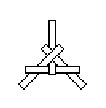
\includegraphics{provlavk}\\

\noindent
Dvě stejné číše jsou naplněny až po čárku, označující 
míru - jedna vínem a druhá limonádou. Vezmeme-li z~číše 
naplněné limonádou plnou lžíci a dáme-li její obsah do číše s~vínem, 
promícháme ji a pak opět plnou lžíci této směsi dáme do limonády, 
bude v~číši s~vínem větší procento limonády než 
procento vína v~číši s limonádou?\\[1 mm]
{\sl V~číši s~vínem bude stejné množství limonády,
jako množství vína v~číši s~limonádou.}\\

\noindent
Kde je na světě místo čtyř světových stran jen jedna 
světová strana?\\[1 mm]
{\sl Na severním pólu je jen jih, neboť kam se podíváme, je to 
vždy jižním směrem. Podobně je na jižním pólu jenom sever.}\\

\noindent
Jak je možno udělat ze dvou tyčí deset, aniž by se zlomily.\\[1 mm]
{\sl Dáme-li dvě tyče přes sebe, vznikne X, římsky 10.}\\

\noindent
Je v~moři více písku nebo ryb?\\[1 mm]
{\sl V~moři je více ryb, písek je pod mořem.}\\

\noindent
,,Závodník snědl tři vejce na lačný žaludek a pak se rozběhl.`` 
Ve větě je chyba. Kde?\\[1 mm]
{\sl Závodník mohl sníst na lačný žaludek jen jedno vejce, při
dalších už nebyl žaludek lačný.}\\

\noindent
V~knihovně jsou zařazeny tři díly jistého šíleného 
románu. Mají 296, 274 a 548 stran. Každý list je silný 0,12 mm 
a jedna deska s~předsádkou 2 mm. Jaká je vzdálenost od 
prvé strany prvého dílu k~poslední straně druhého dílu?\\[1 mm]
{\sl Vzdálenost je 4 mm. Horní deska s~předsádkou prvního 
dílu a spodní deska s~předsádkou druhého dílu.}\\

\noindent
Majitel ranče odkázal majetek svým třem synům, přičemž 
stanovil, že se o 17 koní mají rozdělit tak, že nejstarší syn 
obdrží polovinu, prostřední polovinu a nejmladší devítinu. Synové 
se málem umlátili, protože jim dělení nějak nevycházelo. Sousedi 
na ně zavolali šerifa, který přijel brzy na rychlém ryzáku a 
snadno dědictví rozdělil. Jak to udělal?\\[1 mm]
{\sl Šerif přidal k 17 koním svého ryzáka, takže jich bylo 18. 
Z~nich dal polovinu (9) nejstaršímu, třetinu (6) prostřednímu,
devítinu (2) nejmladšímu synovi a svého koně si vzal zase zpět.}\\

\noindent
V~kolik hodin rozdělují ručičky hodinek ciferník 
na dva půlkruhy, v~nichž je v~každém stejný součet 
hodin (tj. součet čísel od 1 do 12)?\\[1 mm]
{\sl Přibližně v 9:17 a 3:49. Součty činí vždy 39.}\\

\noindent
Kupující platil za klobouk, který stál 50,- stokorunou. 
Protože obchodník neměl nazpět, šel bankovku rozměnit nazpět 
do blízké drogerie a pak návštěvníkovi vrátil 50,- Druhého dne 
se drogista přihlásil, že stokoruna je falešná a obchodník mu 
musel dát jinou. Jakou celkovou škodu obchodník utrpěl?\\[1 mm]
{\sl Přišel celkem o 100,- které musel dát drogistovi místo falešné 
stokoruny. Za klobouk mu zůstalo 50,- od drogisty.}\\

\noindent
Bystrý je-li luštitel náš mladý, neztroskotá v~tomto 
taji. 85 let dohromady dědeček s~vnukem prý mají. O 65 let přitom
děda více má než vnouče jeho. Jak stár je vnuk řešení se hledá,
není to nic nesnadného.\\[1 mm]
{\sl Vnukovi je 10 a dědovi 75.}\\

\noindent
Dá-li Frantík Pepíkovi dvě kuličky, bude mít Pepík dvakrát 
tolik kuliček co Frantík. Dá-li Pepík Frantíkovi dvě kuličky, 
budou mít oba stejný počet. Kolik kuliček má Frantík a kolik 
Pepík?\\[1 mm]
{\sl Frantík má 10 kuliček a Pepík 14.}\\

\noindent
Napište jedním slovem suchá tráva.\\[1 mm]
{\sl Seno.}\\

\noindent
Co je mezi mořem a zemí?\\[1 mm]
{\sl Písmeno ,,a''.}\\

\noindent
Čtyřicet bez deseti je padesát. Jak je to možné?\\[1 mm]
{\sl V~římských číslicích: XL - X = L}\\

\noindent
Dobře se zamyslete a odpovězte. Je dříve dům postaven 
nebo zbourán?\\[1 mm]
{\sl Dům je dříve postaven, neboť bourat jej můžeme až po postavení.}\\

\noindent
,,Dcera se už bude vdávat, ačkoliv jsme slavili pětkrát 
její narozeniny a žádné jsme nevynechali,'' prohlásil tajuplně 
otec. Jak je to možné?\\[1 mm]
{\sl Dcera se narodila 29. února, má tedy narozeniny co 4 roky.}\\

\noindent
Je možné, aby polovina z 12 bylo 7?\\[1 mm]
{\sl V~římských číslicích dostaneme podélným rozpůlením 
čísla XII číslo VII.}\\

\noindent
Kterou rostlinu pozná snadno i slepý?\\[1 mm]
{\sl Kopřivu.}\\

\noindent
Čeho je v~kalamáři nejvíce?\\[1 mm]
{\sl Písmene ,,a''.}\\

\noindent
Dva otcové a dva synové byli na návštěvě. Při svačině 
před ně hostitelka předložila tři čaje a vybídla je, aby pili. 
Všichni najednou se napili. Jak je to možné?\\[1 mm]
{\sl Jsou to dědeček, syn a vnuk (tedy pouze tři osoby).}\\

\noindent
Dvanáct mincí leží jako na číselníku hodin. Vašim úkolem je 
přemístit mince tak, aby od 1 do 6 ležely dvě mince na sobě. 
Mince se přemisťují skokem přes dvě mince ležící vedle.\\[1 mm]
{\sl 12$\rightarrow$3, 7$\rightarrow$4, 10$\rightarrow$6, 8$\rightarrow$1, 
9$\rightarrow$5, 11$\rightarrow$2}\\

\noindent
V kruhu leží 18 zápalek a jako 19 je krabička. Vašim úkolem 
je odkudkoli odpočítat 6 sirek, šestou vzít a počítat dál, až 
zůstane pouze krabička. S krabičkou se pracuje stejně jako se 
sirkami.\\[1 mm]
{\sl Jako první se vezme 11. Zápalka od krabičky.}\\

\noindent
Vyjmenujte 5 po sobě jsoucích dnů, jejichž jméno neobsahuje 
U ani K.\\[1 mm]
{\sl Předevčírem, včera, dnes, zítra, pozítří}\\

\noindent
Jak udělat ze čtyř karetních pětek čtyři čtverky. Některou 
kartou něco zakrýt.\\[1 mm]
{\sl Karty se položí do kříže (kruhu), každá karta zakrývá své 
sousedce jeden znak.}\\

\noindent
Jak položit na stůl tři sirky tak, aby se hlavičkami 
nedotýkaly stolu.\\[1 mm]
{\sl Utvoříme ze sirek trojúhelník, přičemž každá sirka bude za 
hlavičkou opřená o sirku vedlejší.}\\

\noindent
Mají v USA 1. máj?\\[1 mm]
{\sl Ano, vždy po 30. dubnu.}\\

\noindent
Kolik dnů narození zažije průměrně člověk?\\[1 mm]
{\sl Pouze jeden, v porodnici.}\\

\noindent
Některé měsíce mají 31 dnů, kolik jich má 28 dnů?\\[1 mm]
{\sl Všechny, tedy 12.}\\

\noindent
Je těžší kilo železa, nebo kilo peří?\\[1 mm]
{\sl Stejně, pokud vám nespadnou na nohu.}\\

\noindent
Je u nás legální oženit se znova se svou ovdovělou
manželkou?\\[1 mm]
{\sl Ne, protože muž, jehož žena je vdova, je mrtev.}\\

\noindent
Vydělte 30 číslem 1/2 a přičtěte 10. Kolik vám vyšlo?\\[1 mm]
{\sl 70, protože 30 děleno 1/2 je 60.}\\

\noindent
Když na misce leží 3 jablka a dvě odeberete, kolik jablek máte?\\[1 mm]
{\sl Dvě. Ty, co jste odebrali.}\\

\noindent
Doktor vám dal tři pilulky a řekl, že máte brát každou půlhodinu
jednu. Kolik minut uteče od první pilulky než si vezmete poslední?\\[1 mm]
{\sl 60. Začnete první pilulkou, o 30 minut později vezmete druhou
a po 30ti minutách poslední.}\\

\noindent
Farmář měl 17 ovcí a kromě devíti mu všechny pošly. Kolik mu
jich zůstalo?\\[1 mm]
{\sl 9, ostatní přece uhynuly.}\\

\noindent
Kolik zvířat každého pohlaví a druhu vzal Mojžíš na svou Archu?\\[1 mm]
{\sl Žádné, to přece nebyl Mojžíš, ale Noe.}\\

\noindent
Kolik dvoukorun je v tuctu?\\[1 mm]
{\sl 12 dvoukorun v tuctu dvoukorun.}\\

\noindent
Na jezírku rostou lekníny. Každé ráno se na hladině objeví $2\times$
tolik leknínů, než kolik tam bylo minulý den. Jezírko úplně zaroste
za 4 dny. Za jak dlouho bude porostlé jen z $1/4$?\\[1 mm]
{\sl Za 2 dny.}\\

\noindent
Napište pomocí šesti číslic 5 a základních aritmetických operátorů
(+ - * /) číslo 1000?\\[1 mm]
{\sl $(5+5)(5+5)(5+5)=1000$.}\\

\noindent
Doplňte číslice 0--9 místo písmenek. Každé písmeno reprezentuje 
jinou číslici: TO + TO + LÉTO + ALE = LETÍ.\\[1 mm]
{\sl 32 + 32 + 4532 + 041 = 4637}\\

\noindent
Doplňte číslice 0--9 místo písmenek. Každé písmeno reprezentuje 
jinou číslici: HLE + HAD + LEZE + NA = ZEMI.\\[1 mm]
{\sl 473 + 406 + 7383 + 90 = 8352}\\

\noindent
Doplňte číslice 0--9 místo písmenek. Každé písmeno reprezentuje 
jinou číslici: DÁME + SI + DO = NOSU.\\[1 mm]
{\sl 6941 + 52 + 60 = 7053}\\

\noindent
Dvojice robotů stojí před naprosto stejnými dveřmi. Jeden ze strojů na tebe
obrátí pohled a řekne: ,,Pravé dveře jsou ty, které potřebuješ.''\\
,,Neposlouchej ho,'' radí ti druhý, ,,lže.''\\
,,Ale jenom někdy,'' reaguje první.\\
Kterými dveřmi půjdeš? Ze [\ref{gabook1}].\\[1 mm]
{\sl Máš jít pravými.}\\

\noindent
Mám tři zlaté truhlice. V každé z nich jsou tři stříbrné truhlice. V každé
stříbrné jsou dvě olověné truhlice. V každé olověné truhlici jsou tři dřevěné
truhlice, ve kterých už žádné truhlice nejsou. Do každé truhlice jsem vložil
jeden zlaťák a ještě tolik zlaťáků, kolik je v ní celkem všech truhlic. Kolik
mám zlaťáků ve všech truhlicích dohromady? Ze [\ref{gabook2}].\\[1 mm]
{\sl $3((1+3(1+2(1+3)))+3((1+2(1+3))+2((1+3)+3))) = 291$}\\

\noindent
Všichni duchové jsou strašidla a někteří duchové jsou obludy. Některé obludy
jsou lidožrouti, takže všichni lidožrouti jsou strašidla. Je to pravda,
nebo ne? Ze [\ref{gabook2}].\\[1 mm]
{\sl Nelze rozhodnout.}\\

\noindent
Mám dvě dcery. Až bude ta mladší tak stará, jako byla starší, když se mladší
narodila, bude zároveň dvakrát starší než je teď. Jaký je jejich věkový
rozdíl, když jim dohromady je 48 let? Ze [\ref{gabook2}].\\[1 mm]
{\sl Rozdíl činí 24 let.}\\

\noindent
Před půl hodinou bylo tři čtvrtě na osm. Kolik bude za hodinu?\\[1 mm]
{\sl Čtvrt na deset.}\\

\noindent
Ve škole je jedna vyučovací jednotka dlouhá 45 minut. Žáci mají 6 vyučovacích
jednotek denně. Kolik hodin se každý den učí?\\[1 mm]
{\sl Čtyři a půl hodiny.}\\

\noindent
Tramvaj přijíždí na zastávku každých 12 minut. První přijela v 9 hodin a 1
minutu. V kolik hodin přijede třetí tramvaj?\\[1 mm]
{\sl V 9 hodin, 25 minut.}\\

\noindent
Nádraží je od mého domu vzdáleno 6 kilometrů. Na kole jezdím rychlostí
12 km/h. Stihnu vlak, jestliže vyjedu 25 minut před jeho odjezdem?\\[1 mm]
{\sl Nestihnu, cesta na nádraží mi trvá 30 minut.}\\

\noindent
Vlak, který měl 20 minut zpoždění, přijel v 8 hodin a 12 minut. V kolik
hodin měl podle jízdního řádu vlak přijet?\\[1 mm]
{\sl V 7 hodin, 52 minut.}\\

\noindent
Za 6 minut bude tři čtvrtě na pět. Kolik bylo před 9 minutami?\\[1 mm]
{\sl Byly 4 hodiny, 30 minut.}\\

\noindent
Jsi v místnosti s jedinými dveřmi. Stojí zde tři sochy: medvěd, vlk
a ještěr. Klíč od dveří je v tlamě jedné ze soch. Musíš tam sáhnout a
klíč vytáhnout. Pokud sáhneš do tlamy, ve které klíč není, socha ti
ukousne ruku.\\
Pod sochami je 6 celkem nápisů, na každém podstavci dva. Na jednom
podstavci jsou oba nápisy nepravdivé, na dalším jsou oba pravdivé a na
zbývajícím je jeden nápis pravdivý a jeden nepravdivý.\\
U vlka je napsáno: ,,Já klíč nemám,'' a ,,Klíč je v tlamě medvěda.'' U
medvěda stojí: ,,Vlk nemá klíč,'' a ,,Klíč najdeš u ještěra.'' Nápisy pod
ještěrem hlásají: ,,Já klíč nemám,'' a ,,Klíč má vlk.''\\
Do které tlamy sáhneš pro klíč?\\[1 mm]
{\sl Klíč je v tlamě ještěra.}\\

\noindent
Na břehu řeky stojí farmář s ovcí, vlkem a hlávkou zelí. U břehu kotví jedna
malá loďka. Loďka je tak malá, že se do ní s farmářem vleze už buď jen koza,
jen vlk, nebo jen zelí.\\
Farmář chce dopravit všechen svůj majetek na druhou stranu. Protože ale vlci
žerou kozy a kozy mají rády zelí, nesmí zůstat bez farmáře na stejném břehu
vlk s kozou, ani koza se zelím.\\
V jakém pořadí má farmář svůj majetek převézt?\\[1 mm]
{\sl Koza tam -- vlk tam -- koza zpět -- zelí tam -- koza tam.}\\

\noindent
Na břehu řeky stojí 3 misionáři a 3 kanibalové. U břehu kotví dvojmístná
loďka. Všichni se chtějí dostat ve zdraví na druhou stranu. Zůstane-li na
jednom břehu více kabibalů než misionářů, kanbalové misionáře seřerou.\\
V jakém pořadí mají jezdit loďkou?\\[1 mm]
{\sl Dva kanibalové tam -- jeden kanibal zpět -- dva misionáři tam -- 
kabibal s misionářem zpět -- dva kanibalové tam -- jeden kabibal zpět --
dva kanibalové tam.}\\

\noindent
Na břehu řeky stojí pětičlenná rodina (syn, dcera, matka, otec a děda).
Přes řeku vede úzká kláda, přes kterou mohou jít současně nejvýše dvě osoby.
Každá osoba přejde přes kládu za jinou dobu. Synovi to trvá 1 vteřinu, dceři
2, matka přejde kládu za 6 vteřin, otec za 8 a děda za 12. Jdou-li dvě osoby
spolu, jdou rychlostí toho pomalejšího.\\
Protože je noc, musí mít ti, co jdou přes kládu, s sebou petrolejku. V lucerně
je ale palivo jen na 30 vteřin.\\
V jakém pořadí musí členové rodiny chodit přes kládu, aby se všichni stihli
dostat na druhou stranu, než lucerna zhasne?\\[1 mm]
{\sl Syn(1) a dcera(3) tam -- dcera(3) zpět -- otec(8) a děda(12) tam -- 
syn(1) zpět -- syn(1) a matka(6) tam -- syn(1) zpět -- syn(1) a dcera(3)
tam.}\\

\noindent
Aby získal ruku šachové princezny, musí princ na šachovém koni splnit nelehký
úkol. Zvolí si libovolné z políček na obrázku. Z něj pak musí skákat z
políčka na políčko tak, aby navštívil všechna ostatní políčka právě jednou
a posledním skokem se vrátit zpět na výchozí pole.\\
Žádné z políček (kromě prvního) nesmí navštívit dvakrát. V jakém pořadí
musí princ po políčkách skákat? Šachový kůň skáče vždy o dvě políčka dopředu
a jedno políčko doprava nebo doleva.\\[1 mm]
\begin{picture}(110,50)(0,0)
 \put(0,39){\framebox(10,10){}} \put(13,39){\framebox(10,10){}} \put(26,39){\framebox(10,10){}} \put(39,39){\framebox(10,10){}}
 \put(0,26){\framebox(10,10){}} \put(13,26){\framebox(10,10){}} \put(26,26){\framebox(10,10){}} \put(39,26){\framebox(10,10){}}
 \put(0,13){\framebox(10,10){}} \put(13,13){\framebox(10,10){}} \put(26,13){\framebox(10,10){}} \put(39,13){\framebox(10,10){}}
 \put(13,0){\framebox(10,10){}} \put(26,0){\framebox(10,10){}}
 \put(60,39){\framebox(10,10){10}} \put(73,39){\framebox(10,10){13}} \put(86,39){\framebox(10,10){6}} \put(99,39){\framebox(10,10){3}}
 \put(60,26){\framebox(10,10){5}} \put(73,26){\framebox(10,10){2}} \put(86,26){\framebox(10,10){9}} \put(99,26){\framebox(10,10){12}}
 \put(60,13){\framebox(10,10){14}} \put(73,13){\framebox(10,10){11}} \put(86,13){\framebox(10,10){4}} \put(99,13){\framebox(10,10){7}}
 \put(73,0){\framebox(10,10){8}} \put(86,0){\framebox(10,10){1}}
\end{picture}\\

\end{multicols}
\clearpage

% End of file


 % Written by Petr Gotthard
% Codepage ISO-8859-2

\section{Kvízové otázky}
\begin{multicols}{\value{columnsthindata}}

\noindent
Tvarovat je\\
a) vyrábět tvaroh\\
b) tvářit se jako tvárnice\\
\textbf{c) dávat tvar nějakému předmětu}\\

\noindent
Kompost je\\
\textbf{a) hnojivo ze zbytků}\\
b) řecky ,,kompot''\\
c) kombinovaný poštovní balík\\

\noindent
Biologicky rozložitelný je\\
a) rozložená učebnice biologie\\
\textbf{b) produkt, který se lehce rozkládá v~přírodě}\\
c) rozkládací sedadlo v~kině\\

\noindent
Čistící stanice je\\
\textbf{a) místo, kde se čistí voda}\\
b) myčka aut v~servisu\\
c) stanice metra, kde dýcháme čistý vzduch\\

\noindent
Gravitace je\\
a) čistý vzduch\\
\textbf{b) zemská přitažlivost}\\
c) latinsky ,,rytina''\\

\noindent
Recyklování je\\
a) výměna pneumatik u bicyklu\\
b) oprava dráhy pro cyklisty\\
\textbf{c) přeměna použitého materiálu na novou základní surovinu}\\

\noindent
Nezfalšovatelné označuje\\
\textbf{a) něco, co nemůžeme napodobit}\\
b) věc, kterou lze těžko provést\\
c) někoho, koho nelze nikdy podplatit\\

\noindent
Svazek je\\
\textbf{a) soubor svázaných předmětů}\\
b) zkratka svazu ekonomů\\
c) svačina z~eidamu a kopru\\

\noindent
Papyrus je\\
\textbf{a) latinské slovo označující papír}\\
b) ruský dědeček\\
c) papírový pytel plný švábů rusů\\

\noindent
Braillovo písmo je\\
\textbf{a) písmo určené nevidomým}\\
b) rukopis irského mnicha\\
c) písmo, kterým je vytištěna nejstarší kniha světa\\

\noindent
Typy jsou\\
\textbf{a) písmena nebo znaky připravené k~tisku}\\
b) stany prérijních Indiánů\\
c) nepříjemní lidé\\

\noindent
Ve vesmíru máme\\
\textbf{a) rudý obličej}\\
b) vzduch\\
c) vodu\\

\noindent
Aerodynamika je\\
a) rychlý sport\\
\textbf{b) věda o odporu vzduchu}\\
c) prehistorický motýl\\

\noindent
Piktogram je\\
a) váha menší než jeden gram\\
b) latinsky ,,zloděj obrazů``\\
\textbf{c) kresba skrývající nějaký význam}\\

\noindent
Čočky jsou\\
\textbf{a) sklíčka nahrazující brýle}\\
b) malé hnědé luštěniny\\
c) čokoládové vločky\\

\noindent
Náprava je\\
a) nádrž právě naplněná\\
\textbf{b) příčná součástka, jež drží kola}\\
c) dopravní značka ukazující doprava\\

\noindent
Vrtačka je\\
a) dívka, která všechno pokazí (zvrtá)\\
\textbf{b) nástroj sloužící k~vrtání}\\
c) středověká dětská hra\\

\noindent
Vodní hodiny jsou\\
\textbf{a) příbuzné hodin přesýpacích}\\
b) čas strávený ve vodě\\
c) stroj na měření času používaný vodníky\\

\noindent
Mikroprocesor je\\
\textbf{a) elektronický mozek}\\
b) zpěvák, který nikdy nezpívá bez mikrofonu\\
c) mikrob, který procestoval svět\\

\noindent
Integrovaný obvod je\\
\textbf{a) elektronický mozek}\\
b) závodní dráha formule 1\\
c) obvod hlavy génia\\

\noindent
Co jsou to patáky ?\\
\textbf{a) Moravsky ,,lékařské prášky``}\\
b) Vysoké jezdecké boty\\
c) Valašské krojové klobouky\\

\noindent
Jak často nastává příliv?\\
a) 1 krát denně\\
\textbf{b) 2 krát denně}\\
c) 2 krát za měsíc\\

\noindent
Čemu se říká opičí hlavolam?\\
a) Tropický pavouk\\
b) Rozcvičovací cvik mimů\\
\textbf{c) Strom blahočet chilský}\\
(má tak rostlé větve, že na něj ani opice nemohou vylézt)\\

\noindent
Jak vytvářejí včely vosk?\\
\textbf{a) Zadečkem}\\
b) Vyvrhují jej ústním otvorem\\
c) Míšením slin s~pryskyřicí stromů\\

\noindent
Šachy pocházejí z \\
a) Arábie\\
\textbf{b) Indie}\\
c) Persie\\

\noindent
První poštovní známky byly roku 1840 vydány v \\
a) Rakousku\\
b) Francii\\
\textbf{c) Anglii}\\

\noindent
Bůh Radegast symbolizoval podle starých Slovanů \\
\textbf{a) Slunce, oheň}\\
b) Bojovníka\\
c) Pokušitele\\

\noindent
Pověst vypráví, že jméno hotelu Zlatá Husa na Václavském náměstí 
vzniklo podle \\
a) Zlatého pokladu ve tvaru husy nalezeného ve sklepení\\
\textbf{b) Přihlouplé dcery tamního hostinského}\\
c) Gurmánské speciality\\

\noindent
Jezuitský řád byl založen \\
a) Sv. Augustinem\\
b) Sv. Dominikem\\
\textbf{c) Sv. Ignácem z~Loyoly}\\

\noindent
Kolik mostů bylo v~Praze na počátku 19. století\\
\textbf{a) 1}\\
b) 2\\
c) 3\\

\noindent
Šampaňské se poprvé podávalo ve století \\
a) 10.\\
\textbf{b) 17.}\\
c) 18.\\

\noindent
Muslimský svátek Ramadán trvá\\
a) Týden\\
b) 14 dnů\\
\textbf{c) Měsíc}\\

\noindent
Benátský cestovatel Marco Polo podnikl se svým otcem a~strýcem 
cestu do Číny ve století\\
a) 12.\\
\textbf{b) 13.}\\
c) 14.\\

\noindent
První film Charlieho Chaplina nese název\\
\textbf{a) Chaplin si vydělá na živobytí}\\
b) Kid\\
c) Chaplin tulákem\\

\noindent
Hora Říp je z \\
a) Žuly\\
b) Břidlice\\
\textbf{c) Čediče}\\

\noindent
Románská rotunda na vrcholu hory Říp se jmenuje rotunda\\
\textbf{a) Sv. Jiří}\\
b) Sv. Vojtěcha\\
c) Sv. Václava\\

\noindent
Hvězdu Aldebaran by jste hledali v~souhvězdí\\
\textbf{a) Býka}\\
b) Berana\\
c) Orla\\
(je nejjasnější hvězdou)\\

\noindent
Který z~uvedených kopců je nejvyšší?\\
a) Milešovka (České středohoří)\\
\textbf{b) Praha (Brdy)}\\
c) Javořice (Českomoravská vysočina)\\
(Praha 863, Milešovka 837, Javořice 837)\\

\noindent
Kokoška pastuší tobolka kvete\\
a) Modře\\
b) Žlutě\\
\textbf{c) Bíle}\\

\noindent
David Livingstone, slavný cestovatel se proslavil svými cestami 
po\\
\textbf{a) Africe}\\
b) Austrálii\\
c) Polárních končinách\\

\noindent
Známé soustroví Galapagos leží svou větší částí\\
\textbf{a) Jižně od rovníku}\\
b) Severně od rovníku\\

\noindent
Přívlastek NEVALNÝ vznikl v~souvislosti se\\
\textbf{a) Zmačkanou látkou, která se špatně válela}\\
b) Latinským ,,valere'', mít hodnotu\\
c) Záporem slovesa volit\\

\noindent
Slovo MANŽEL vzniklo ze\\
a) Staroněmeckého ,,Mannesseele'' (mužská duše)\\
b) Francouzského ,,manchelle'', což byl mužský svatební kabát 
s~dlouhými rukávy\\
\textbf{c) Staročeského ,,malženstvo'' (mladoženství)}\\
(označovalo jak manželský stav tak i~celý pár)\\

\noindent
Krápavka je \\
a) Krápníkový útvar vzniklý prokapáváním vody uvnitř staveb, 
např. tunelů\\
b) Drobná žába žijící ve středomoří\\
\textbf{c) Skleněná trubička používaná v~laboratořích pro 
odkapávání drobných kapek (pipeta)}\\

\noindent
Slovo POTENTÁT (tj. panovník nebo významný hodnostář) má následující 
původ\\
a) Každý se z~něj potentuje\\
b) Z~latinského ,,potens'' (mocný)\\
c) Z~německého ,,Bodenteider'' (ochránce země)\\

\noindent
Slovo KLUK původně označovalo\\
a) Luk\\
\textbf{b) Šíp}\\
c) Sekeru používanou pro klučení lesů\\
(neopeřený šíp, který daleko nedoletí, později přeneseno na nezralou 
mládež)\\

\noindent
Baldachýn se jmenuje podle\\
\textbf{a) Bagdádu, odkud byla dovážena na něj látka}\\
b) Čínských bálů, francouzsky ,,Bal de Chine''\\

\noindent
Cereálie jsou\\
a) Sušené celerové kostičky\\
\textbf{b) Obilniny}\\
c) Druh mořských sasanek\\

\noindent
Glycidy jsou pro organismus zdrojem\\
\textbf{a) Energie}\\
b) Vody\\
c) Glycerinu\\

\noindent
Z celkového denního energetického příjmu by měla snídaně tvořit\\
\textbf{a) 20 \%}\\
b) 30 \%\\
c) 50 \%\\

\end{multicols}
\clearpage

% End of file

 \section{Kouzlení a čarování}

\subsection{Pomůcky}

Kouzelnická hůlka je dřevěná, kulatá 30 cm dlouhá tyčka. Celá 
černě lakovaná, jen 6 cm obou konců je bílých.

\subsection{Kouzla humorná}

\nadpis{Fakir}{cokouzla}
Palec překryji šátkem a začnu do něj bodat jehlice a 
špendlíky. Pak je zase vytahám, palec odkryji a vše je v~naprostém 
pořádku.

Palec z~rukavice něčím vycpaný je jemně nastehován 
na šátek. Když palec přikrývám, pod kapesníkem palec ohnu a do 
prstů sevřu spodní konec látkové napodobeniny. Napodobenina musí 
být vždy schovaná v~šátku, divák ji nesmí vidět.


\nadpis{Jasnovidec}{cokouzla}
Řekneme, že uhádneme, co si kdo myslí. Do řady postavíme 
tři dobrovolníky a připravíme tři mince. Prvnímu dobrovolníkovi 
řekneme: ,,Dám vám teď minci, pevně ji sevřete v dlani.`` A dáme 
mu minci. U druhého postup zopakujte. Třetímu však nic neříkejte, 
jen viditelně držte poslední minci. Divák otevře dlaň a nastaví 
ruku. Ukažte na něj hůlkou a řekněte: ,,Tento divák si myslí, 
že také dostane minci.``


\nadpis{Jasnovidka}{cokouzla}
Kouzelnice požádá několik diváků, aby napsali na papír 
několik slov. Oni pak odevzdají asistentce, která je složí, vloží 
do klobouku a odevzdá jasnovidce. Ta papíry vytahuje, čte slova 
a říká, zda je psala žena či muž.

Trik spočívá ve skládání papíru. Papír lze nejprve přehnout 
ve svislé nebo ve vodorovné ose. Podle toho jasnovidka pozná 
pisatele.


\nadpis{Jasnovidec}{cokouzla}
Diváci se domluví na nějakém slově a já je uhádnu.

Kouzelník ukazuje náhodně na diváky a ti mají za úkol říkat 
různá slova. Kouzelník je však domluven s~pomocníkem, 
který říká slova, jejichž první písmeno je vždy obsaženo v hledaném 
slově. Je-li slovo celé, řekne pomocník předem dohodnuté slovo.

Př. Slovo=řemen, pomocník hlásí Řád, Eskymák, Mlha, Ešus, Noha.


\nadpis{Kuličky}{cokouzla}
Z papíru 3$\times$3 cm utvořte tři kuličky a položte si je do 
žlábku mezi dvěma prsty. Pak foukněte a všechny kuličky spadnou. 
Teď se zeptejte, která kulička má zůstat na svém místě při dalším 
fouknutí. Zamávejte nad ní hůlkou,přidržte ji a foukněte. Diváci
pochopí žert, vy však buďte ochoten pokus opakovat s jinou kuličkou.


\nadpis{Kolik je 7$\times$7}{cokouzla}
Utvoříme si kartičku 7$\times$7 a rozstříháme ji podle prvního
obrázku. 7$\times$7 je teď 49. Poskládáme-li však rozstříhanou
kartičku podle druhého obrázku, přesně jeden čtvereček bude
chybět. 7$\times$7 je tedy 48.\\
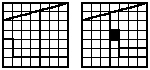
\includegraphics{kolik7x7}


\nadpis{Pravopisný chyták}{cokouzla}
Ať se přihlásí ten, kdo si myslí, že zná dobře český pravopis. 
Nadiktujeme mu pak k napsání tuto větu: Kočí zvedl bič a zvolal: 
Hyje, koníčky...  (na konci mlaskneme jazykem jako na koně). 
Mlasknutí se ještě nikomu nepodařilo napsat a ani nepodaří.


\nadpis{Silné nervy}{cokouzla}
,,Kdo z vás vydrží pod stolem do kterého 3x za sebou prudce 
udeřím dlaní?'' Určitě se nikdo najde a vleze si pod stůl. Ty 
pak udeř do stolu ale jen dvakrát. ,,Tu třetí ránu dám až za 
týden, jsem sám zvědav, jestli odvážlivec tam tak dlouho vydrží 
!''


\subsection{Kouzla vážná}

\nadpis{Prostupnost hmoty}{cokouzla}
Mám šňůrku a na jejích koncích korálky. Vezmu sklenici 
s~velkým uchem dnem vzhůru. Šňůrku položím na levou ruku 
tak, že její střed spočívá mezi nataženým palcem a ukazováčkem 
a tvoří mezi nimi proužek. Na šňůrku položím ucho sklenice, zatlačím, 
korálky se mírně zvednou. Pak sklenici pustím a ona zůstane viset.

Když tlačíme ucho proti šňůrce a tím vytahujeme korálky, 
vyprostíme palec, takže stuha visí je na ukazováku. Poté vsuneme 
ucho mezi palec a šňůrku a vsuneme palec uchem zase pod šňůrku. 
Tlačíme dál, až se nám dostanou korálky do dlaně. Teď sklenici 
pustíme. Jeden korálek se provleče uchem, šňůrka se napne a sklenice 
zůstane viset.


\nadpis{Čtenář myšlenek}{cokouzla}
Oznámíte všem, že jste čtenář myšlenek, o čemž je hned 
přesvědčíte. Vyzvete je, aby každý napsal na list papíru nějaké 
přísloví nebo libovolnou větu o pěti slovech (ne více), dal ji 
do obálky a zalepil. Potom obálky seberte, jednu po druhé přikládejte 
na čelo, soustředíte se, tváříte se důmyslně a k úžasu přítomných 
čtete věty v nich obsažené.

Je třeba abyste byli předem smluveni s některým z hráčů. 
Když přiložíte první obálku na čelo, nevíte sice co je v ní napsáno, 
ale znáte větu, kterou jste si předem smluvil se svým tichým 
společníkem a tuto větu řeknete jako první. Když pak obálku ,,pro 
kontrolu'' otvíráte, seznámíte se s obsahem věty, kterou 
napsal jiný účastník a přisoudíte ji další obálce. Po skončení 
celé atrakce se mohou účastníci přesvědčit, že všechny věty, 
které jste přečetl, jsou skutečně na lístcích napsány. Při otvírání 
obálek je nutno dát bedlivý pozor, abyste obálku se smluvenou 
větou otevřeli jako poslední. Je dobře, když obálky i lístky 
papíru jsou stejné, aby některý z diváků nepoznal trik. Pokud 
chceme ušetřit obálky, musí všichni hráči svůj papír složit stejným 
způsobem a to tak, aby nebyl vidět text.


\nadpis{Sirky ve vzduchu}{cokouzla}
Ukážu ruce, sáhnu do vzduchu a objevím sirku, hodím 
ji do klobouku a už vytahuji za zády další sirku, kterou opět 
házím do klobouku a to už... Pak z klobouku vysypu celou hrst 
sirek

Z průhledné lepicí pásky si zhotovím lepicí prstýnek a nasadím 
na prostředník. Jakmile ukážu ruce, nalepím na prstýnek ze strany 
nehtu sirku. Jsou-li prsty nataženy, sirka není vidět. Hmátnu 
tedy do vzduchu, skrčím prsty a objevím sirku. Objevenou sirku 
přidržím palcem. Ruku vstrčím do klobouku, kde prsty narovnám. 
Tím se sirka zase schová a já ji mohu zase někde najít. Nakonec 
sirku palcem odlepím, hodím tentokráte doopravdy do klobouku 
a z klobouku vysypu sirky, co jsem tam měl již nachystány.


\nadpis{Dámy utekly}{cokouzla}
Ukážeme několik karet a mezi nimi dvě dámy. Řekneme, 
že dámy nemají rády, když to a to. Pak karty složíme a převážeme 
gumičkou. Uděláme to a to. Poté gumičku odstraníme a vida, dámy 
jsou pryč. Pak je někde objevíme.

K tomuto kouzlu je nutné si připraviti preparovanou kartu. 
Z obou dam odstřihneme horní pětinu karty a slepíme je k sobě. 
Mezi ostatními kartami (ukazujeme sloupec karet) vypadají normálně. 
Když ale karty skládáme, přehneme preparované dámy a schováme 
je v dlani. Jakmile sáhneme do kapsy pro gumičku, necháme dámy 
v kapse. Před představením někde uschováme dvě normální dámy, 
které pak náhodou objevíme.


\nadpis{Kde je těžiště}{cokouzla}
Kouzelník vezme dlouhou krabičku a z malé části ji položí 
na sklenici, krabička však nespadne.

U jednoho konce krabičky je připevněno olůvko, které přesunuje 
těžiště, takže se sklenice nepřeváží.


\nadpis{Kdo postaví krabičku}{cokouzla}
Prázdná krabička od sirek je položena na kraji stolu 
tak, že ji kousek přečnívá desku stolu. Kouzelník ji zespodu 
jedním prstem postaví. Ukáže krabičku, že je zcela normální. 
Když krabičku zkouší postavit divák, vždy se mu převáží dozadu.

Krabička na stole leží vždy obrázkem nahoru. Je-li dno její 
zásuvky blíže k desce stolu, krabičku lze postavit, je-li však 
zásuvka zasunuta obráceně, krabička se vždy převáží.


\nadpis{Matematický omyl}{cokouzla}
Divák má sčítat po řadě čísla 1000 + 30 + 1000 + 30 + 
1000 + 30 + 1000 + 10. Téměř všichni odpoví, že výsledek je 5000, 
ačkoli je 4100.

Divák prostě podlehne pravidelnosti a svůj omyl si neuvědomí.


\nadpis{Mince je pryč}{cokouzla}
Položíme minci na táce, přikryjeme šátkem a obejdeme 
diváky. Každý vsune ruku pod šátek a řekne, zda tam mince skutečně 
je. Potom uděláme abrakadabra a zvedneme šátek. Mince zmizela. 
Obdobným postupem se mince na tácku opět objeví.

Ke kouzlu je zapotřebí pomocníka, jemuž jako poslednímu tácek 
ukazujeme. Ten minci v první fázi vezme, schová a řekne, že tam 
je. Ve druhé fázi minci na tácek položí a řekne (jako všichni 
ostatní), že tam mince není.


\nadpis{Najdu správnou kartu}{cokouzla}
Karty jsou seřazeny do 3 sloupců po 7 kartách. Divák 
si vybere kartu a ukáže na sloupec, ve kterém se nachází. Totéž 
pak udělá ještě 3x. Pak mu kouzelník slavnostně ukáže jeho kartu.

Karty je nutné sbírat po sloupcích tak, aby divákem označený 
sloupec byl vždy uprostřed. Po třetím posbírání je karta je jedenáctá 
ať se počítá z kterékoli strany.


\nadpis{Očarovaný řetěz}{cokouzla}
Dvojitý řetěz držím ve svislé poloze. Druhou rukou vezmu 
kroužek, pustím jej a on propadne a zastaví se dole jako poslední 
článek řetězu.

Asi ze třiceti kroužků sestavíme řetěz následovně. Do jednoho 
kroužku navlékneme dva další. Pak řetěz přetočíme o 90$^\circ$ 
doprava. Do zadního kroužku navlékneme další kroužek a oběma 
(zadním i předním) provlékneme druhý kroužek. Řetěz opět přetočíme 
o 90$^\circ$ doprava a pokračujeme v sestavování. Do zadního 
kroužku... Poslední kroužek je navléknut do obou kroužků předchozího 
článku.

Palec a ukazovák levé ruky pevně drží jednotlivý horní kroužek. 
Palec a ukazovák pravé ruky uchopí pravý kroužek pravého páru 
(je v něm navléknut pouze jeden kroužek druhého páru) Horní jednotlivý 
kroužek pustíme a ten zdánlivě prostoupí celým řetězem a umístí 
se jako poslední dole. Přitom řetěz přetočíme zase o 90$^\circ$ 
a horní kroužek uchopíme levou rukou. Palec a ukazovák pravé 
ruky uchopí pravý kroužek pravého...


\nadpis{Přimražená sklenice}{cokouzla}
Na sklenici úplně plnou vody přiložíme papír a zrcátko. 
Pak foukneme ,,studený vítr`` a posečkáme. Sklenice za určitou 
dobu přimrzne k zrcátku.

Papír je savý piják, voda převařená. Papír vysává vodu, tím 
vzniká podtlak a sklenice drží.


\nadpis{Sirka dělá stojku}{cokouzla}
Kouzelník má v ruce sirku, postaví ji hlavičkou na podložku, 
pronese kouzelné slovo a sirka stojí.

Potají si nasliníme nehet, ten pak v nestřeženém okamžiku 
třeme o hlavičku sirky, čímž ji navlhčíme. Takováto sirka vydrží 
stát na vhodné podložce (papír, látkový ubrus) velmi dlouho.


\nadpis{Sklenice propadne stolem}{cokouzla}
Kouzelník vezme sklenici, přikryje je ji šátkem. Pak 
nakreslí na stůl křížek a položí sklenici na něj. Sklenice však 
propadne stolem, spadne na zem a rozbije se.

Kartónové kolečko stejného průměru jako vrchol sklenice nastehujeme 
na šátek. Když bereme sklenici pod šátkem, chytneme sklenici 
i kartónek. Ve chvíli, kdy kreslíme křížek, pustíme sklenici 
do klína (díky šátku nepozorovaně). Kartónek stále držíme, takže 
to vypadá, jako by se nic nestalo. Pak už jen stačí, když pokládáme 
,,jako sklenici`` na stůl, pustit z klína sklenici na zem.


\nadpis{Voda mění barvu}{cokouzla}
Ve sklenici je červená voda. Sklenici přikryjeme šátkem, 
zakouzlíme. Když zvedneme šátek, je ve sklenici voda čirá. Přelijeme 
vodu z jedné sklenice do druhé a vida --- voda je zase červená.

Ve sklenici je vložka z červené hmoty vysoká přesně na výšku 
hladiny. Když snímáme šátek, vyjmeme zároveň i vložku, takže 
voda je bílá. Ve druhé sklenici je KMnO$_4$, ten vodu obarví opět 
na červeno.


\nadpis{Výroba zlata}{cokouzla}
Podivným činěním vytvoříme zlato.

Roztok octanu olovnatého v jedné baňce a jodidu draselného 
v baňce druhé zahříváme na teplotu varu. Slijeme obě tekutiny 
barvy čisté vody dohromady. Jakmile začne směs chladnout, objeví 
se na dně krystalky ,,zlata''.


\nadpis{Zmizelé mince}{cokouzla}
Na stole leží mince. Vezmeme plechový tácek, shrneme 
na něj zmiňované mince. Mince při dopadu na tácek zvoní, ale 
když jej ukážeme divákům, nic na něm není.

Asi 10 cm pod úrovní desky stolu je plech. Mince tedy zvoní, 
jako kdyby dopadaly na tácek, ve skutečnosti však dopadají na 
plech.


\nadpis{Modrý --- červený}{cokouzla}
Karetní hru rozevřu do vějíře a ukážu z~obou stran. 
Diváci vidí karetní hru s~modrým rubem. Pak karty shrnu 
do balíčku, modrou kartu odeberu, červenou přidám, karty zase 
rozevřu a už mají rub červený.

Karty preparujeme následujícím způsobem. Oddělíme ruby a 
úhlopříčně je rozstřihneme a pak zase slepíme. Lepíme však tak, 
že na jedné kartě je polovina červeného a polovina modrého rubu. 
Slepené karty zatížíme. Dvě karty takto nepreparujeme. Když karty 
rozevřeme, ukážeme vždy jednu polovinu rubu. Jen horní (jedna 
z~nepreparovaných) je vidět. Pak karty složíme a vodorovně 
odložíme. Poté sejmeme modrou nepreparovanou a nahradíme ji červenou, 
rovněž neupravenou kartou. Mezitím je nutné karty otočit. Když 
vějíř zase rozevřeme, vidí diváci tentokráte druhou polovinu 
rubu preparovaných karet.


\nadpis{Colombovo kouzlo}{cokouzla}
Vyzvěte diváka, aby si myslel číslo od 1 do 4 a pak vám 
je řekl. Na důkaz své jasnozřivosti vyzvěte diváka, aby se podíval 
na určité skryté místo, kde nalezne cedulku: ``Věděl jsem, že 
si myslíte číslo...''.


Na různých skrytých místech jsou umístěny cedulky pro všechna 
přípustná čísla. Podle čísla, které si myslel, vyšle diváka kouzelník 
na místo s~patřičnou cedulkou.


\nadpis{Jasnovidec}{cokouzla}
Vybraný divák si bude myslet číslo od 1 do 4 (lze i více). 
Kouzelník se chvíli soustředí a pak řekne: ,,Už vím, jaké 
číslo si myslíte. Řekněte mi je.'' Divák řekne své myšlené 
číslo. ,,A teď se podívejte pod talíř,'' řekne kouzelník. 
Divák pod talířem nalezne cedulku: ,,Věděl jsem, že si 
myslíte číslo...''

Pokud by divák řekl, že si myslel jiné číslo, poslal by ho 
kouzelník podívat se pod jiný předmět. Kouzelník má totiž připraveny 
pod různými předměty cedulky pro všechna možná čísla. Předmětů 
by mělo být mnohem více než čísel.


\nadpis{Kapsa plná karet}{cokouzla}
Divák vytáhne z~balíčku 3 karty a zapamatuje si 
je. Kouzelník si karty vloží do kapsy, potom dvě vytáhne a požádá 
diváka, aby řekl jednu z~karet, které si vytáhl. Kouzelník 
potom vytáhne z~kapsy třetí kartu --- a je to přesně ta, 
jakou určil divák.

Kouzelník si karty vloží do kapsy a přitom si zapamatuje 
jejich pořadí. Potom vytáhne z~kapsy dvě jiné karty, které 
už v~kapse byly. Jakmile řekne divák své přání, bez problémů 
vytáhne patřičnou kartu.


\nadpis{Létající mince}{cokouzla}
Před zraky diváků postav na prázdnou sklenici talířek. 
Přes všechno pak přehoď šátek. Nyní vezmi do levé ruky korunu 
a dej ji do druhé ruky a zároveň ji vyhoď do výšky. Vezmi kouzelnickou 
hůlku a začni vysvětlovat, že mince lítá ve vzduchu a že jí hůlkou 
stáhneš přes talířek do sklenice. Hůlkou se dotkneš a uvolněná 
mince spadne s cinknutím na dno sklenice.

Při pokládání talířku na sklenici přidrž nenápadně na dně 
talířku přidrž korunu a přimáčkni ji mezi talířek a sklenici. 
Do levé ruky vezmi jinou korunu, naoko ji dej do druhé ruky a 
naznač její vyhození do vzduchu. Mezitím ukliď z levé ruky korunu 
do kapsy. Hůlkou se potom dotkni talířku na okraji, tím ho na 
druhé straně nadzvedneš a mince spadne do sklenice.


\nadpis{Matematický trik}{cokouzla}
Kouzelník předloží kartičku s~čísly. Divák si vybere 
jedno číslo a zatrhne všechna čísla v řádku a sloupci, kde se 
zvolené číslo vyskytuje (10). Pak si vybere číslo ještě nezatržené 
a postup opakuje (4). Součet zbylých čísel je vždy 40.


\nadpis{Pravdomluvné zrcadlo}{cokouzla}
Vyhlídni si předem svou oběť, na kterou napiš křídou 
na zrcadlo nějaký vtip. Vše pak smaž hadrem, takže sklo se jeví 
jako čisté. Pak přede všemi vyzvi svou oběť aby se podívala do 
zrcadla a řekla co vidí. Samozřejmě, že uvidí jen sama sebe. 
Řekni, že zrcadlo je kouzelné, ale ten co se do něj dívá se musí 
napřed otočit 3x doprava, pak 3x doleva a nakonec na zrcadlo 
3x dýchnout. Pak mu zrcadlo něco poví.


\nadpis{Rentgenový zrak}{cokouzla}
Kouzelník se otočí, diváci položí na stůl minci a přikryjí 
ji neprůhledným hrnečkem. Kouzelník se zamyslí a pozná, jaká 
to je mince.

Pomocník a zasvěcenec, který minci přikrývá, nasměruje ouško 
hrnečku směrem podle toho, jaká mince pod hrnečkem je.


\nadpis{Šáteček a svíčka}{cokouzla}
Na stolek připrav větší nezapálenou svíčku a pootevřenou 
krabičku sirek. Svíčku zapálíme a krabičku sirek zavřeme. Hořící 
svíčku chytíme jednou rukou a druhou vytáhneme z~plamene 
šáteček.

Šáteček je nasoukán v~krabičce sirek. Svíčku zapálíme 
a krabičku sirek zavřeme, tím se dostane šátek nepozorovaně do 
dlaně. Není pak už nic snazšího, svíčku chytit rukou se šátečkem 
a druhou jakoby s plamene vytáhnout šáteček.


\nadpis{Zlomená sirka}{cokouzla}
Divák zlomí sirku, kouzelník ji zabalí do kapesníku, 
zakouzlí a divákova sirka je opět celá a neporušená.

Předem (mimo zraky diváků) zasuneme do lemu kapesníku jednu 
sirku. Pak požádáme někoho z diváků, aby nám donesl zdravou zápalku. 
Tu pak před všemi dáme doprostřed kapesníku a poznačíme fixem, 
aby nemohlo dojít k záměně. Pak kapesník překládáme ovšem tak 
šikovně, abychom dali divákovy přes kapesník do ruky sirku v 
lemu. Požádáme ho aby sirku zlomil. Po té kapesník rozbalíme 
a vyndáme a divákům ukážeme opět zdravou sirku.


\nadpis{Živá kouzelnická hůlka}{cokouzla}
Po krátké přednášce o důležitosti kouzelnické hůlky, 
vezmi láhev a hůlku do ní strč. Po magických slovech a pohybech 
volné ruky sama vylézá z~láhve.

Hůlku však předem za jeden konec přivážeme za nit. Ten pak 
strkáme do láhve. Druhý konec nitě zavážeme k opasku kalhot. 
Tím, že pohybujeme lahví, hůlka vystupuje či zajíždí do láhve. 

 % Written by Petr Gotthard
% Codepage ISO-8859-2

\section{Cvičení řeči}
\begin{multicols}{2}

\subsection{Jazykolamy}

\begin{itemize}
\itemsep -3pt

\item[-] Jen mi, kmotře Petře, toho vepře nepřepepřete. Jestli mi 
toho vepře, kmotře Petře, přepepříte, pak si toho vepře, kmotře 
Petře, snězte sám.

\item[-] Letělo tři tisíce tři sta třicet tři stříbrných křepelek přes 
tři tisíce tři sta třicet tři stříbrných střech.

\item[-] Naše lomenice je ze všech lomenic ta nejlomenicovatější.

\item[-] Drbu vrbu.

\item[-] Sel pštros s pštrosicí a s pštrosáčátky Pštrosí ulicí.

\item[-] Naleju-li oleje, nenaleju-li oleje.

\item[-] Já rád játra, ty rád játra.

\item[-] Řekl řek, kolik je v Řecku řek.

\end{itemize}

\subsection{Výslovnost}

\begin{description}
\itemsep 0pt

\item[S] V~sadě se pase husa s~housaty. Sova houká v~lese. 
V~létě spíme ve stanu. Sype, les, maso, sám, snaha, sníh,
písně, miska, píská, kokos, kompas, nos.

\item[Z] Koza leze do zelí. Zuzana veze vozík. Zdeněk má
zelený balón. Je zima. Zima, zebe, zase, zebra, zívá, zisk,
vozí, kazí, kozí, zbojník, zde, zdola, zob.

\item[C] Chlapec běžel na kopec. Koníci cválají do kopce. Alice cinká 
na poklice. Cena, cihla, necky, nic, domácí, ocel, ovoce, cítí, civí,
cibule, lovec, otec, kopec.

\item[S -- C] Malé selátko cucá. Cilka má dlouhé vlasy. Slunce svítí. 
Měsíc svítí v~noci. Cosi, cesta, silnice, slepice, myslivec, ocas,
sice, svícen, slunce, tisíc, soudce.

\item[Z -- S] Na podlaze jsou zase saze. Pes veze vozík. V~zimě 
jezdíme na saních. Zase, saze, zápis, zastaví, zasadí, zásuvka, zásoba, sazenice, svízel, smazal.

\item[C -- Z] Cilka nese záclony. Někdo zcizil peníze. Cizinec zabloudil 
na ulici. Co to cinká? Cizina, cizinec, cizí, zajíc, vzácnost, záclona,
zacpal, horolezec, jezdec, vzácný.

\item[Š] Náš Míša našel v~lese šišku. V~koši byly myšky. Hoši mají tašky.
Koš, máš, náš, voláš, šumák, koše, naše, škola, škytá, výška, jíška,
lepší, ještě.

\item[Č] Anička má ráda čokoládu. Mám míč a bič. Kolotoč se točí. Čpavek 
čpí. Oč, pláč, upeč, čočka, kočka, počká, čokoláda, čouhá, čumák, často,
čepel.

\item[Ž] Želva pomalu leze. Božena má nové lyže. Žížala leží u kaluže.
Žížala, žáci, žehlí, žena, žold, lože, lyže, vlažný, dlažba, dlužen, něžný,
žně.

\item[Č -- Š] Ušáček, Vašíček, košíček, šáteček, češe, čeština, školáček, 
kašička, mašlička.

\item[Ž -- Č] Nožička, žehlička, lžička, mužíček, nožíček, čížek, kůžička, 
žehlička, nožíček.

\item[C -- Č] Čepice, cvičky, cvičí, Aničce, kočce, cvičitel, cvočky, 
čepice, tetičce, kočce.

\item[S -- Š] Sušenka, suší, sešit, sluší, snáší, soška, štěstí, šije 
se, slušně, šťastný, šosy.

\item[Z -- Ž] Zamaže, zaváže, železo, žízeň, zboží, zběžný, žíznivý,
žaluzie, žezlo.

\item[Š -- C] Švec, náušnice, myšce, lišce, o myšce, maceška, ve výšce, 
šicí, pšenice.

\item[S -- Ž] Sváže, sjíždí, složí, spolužák, sněží, snížek, užaslý,
možnosti, žalost, smaží.

\item[Č -- S] Číslo, čistí, slečna, sáček, měsíček, louskáček, sčítá součet, 
svačí, skučí, skoč.

\item[L] Nad lesem letí letadlo. Bylo bláto. Nebyla celá bílá. Slimák 
se schoval. Lípa, loďka, plakal, láme, lano, laň, louka, dál, vál, sál,
ukládá, klopýtá, kluk.

\item[R] Petr pracuje v~továrně. Traktor má silný motor. U hradu 
byl ukrutný drak. Kotrmelec, strašný, vrznout, fraška, brada, brzo, brýle, hromada, hrbol.

\item[Ř] U řeky roste řepa. Stařeček řeže dříví. Zavři pusu, Petříku. Zahřmělo.
Dřímá, truhlář, třpytka, natřásl, příběh, příchod, přijal, přejel, křižovatka.

\item[P] Pavel pracuje v~továrně. Petr propíchl peřinu. Pepa stojí 
pod lípou. Popel, pálí, Petr, pampeliška, pomalu, pec, pivo, popleta,
papoušek, páv.

\item[B] Bába Bulíková šla do lesa na houby. Béďa peče bábovku. Kubu 
bolí zoubek. Bude, bledý, bída, bouda, hubený, houba, obutý, obilí, obálka, 
Kuba, kabát.

\item[D] Máme doma dudy. David jede domů. Teta mi dala domino. Tady je 
dům. Odpoledne, domov, sudy, dudlík, dávno, datum, dech, doutnák, 
doupě, den.

\item[T] Teta stojí u stolu. Kotě v~botě tiše kouká. Potom chytí 
klubko nití. Teče, tulipán, také, kabát, nitky, kvítky, látky, kabátky,
Tonda, boty, tahat.

\item[M] Máma má malé dítě. My máme maso v~míse. Máma mele pro 
mne mák. Moje, med, mísa, Míša, mouka, máma, mnoho, málo, mák, pomocník.

\item[N] Naše Nána nosí noviny. Punťa chňapl po pečeni. Jeník měl sáně.
Noc, nový, nůše, neděle, nehoda, panenka, venku, nenapomene, nechce.

\item[H] Honza Hynek nosí hodinky. Helena hledá houby. Hbitý Haf pobíhá.
Hůl, hádá, hladí, nohy, hádanka, honem, hodnota, houska, hmota, hlava.

\item[CH] Chlapci chodí na chůdách. Hluchý lachtan delfínem je lechtán.
Chová, chechtá, chochol, buchta, chuť, chasa, chapadlo, pech, suchá.

\item[K] Karel Kovář seká sekyrou. Alenka kolébá panenku. Na poli kvete 
mák. Kůň, klepe, kytka, kykyryký, kočka, kotě, kope, koupí, liška,
lžička, puk.

\item[G] Gusta nosí gumové galoše. Gábina dala gól. Magda má guláš.
Gábina, guma, gazela, gepard, gatě, gauč, guláš, gesto, globus, magnetofon.

\item[F] Fouká vítr. Fanda foukal na flétnu. Filípek je filuta. Fujavice 
pofukuje. Fanouš, fazole, fíky, Fanda, fialky, faleš, flanel, flétna, vtip, 
fošna, fontána.

\item[V] Vašek Vítek vozí vozík. Véna veze Vandu. Kvákej: ,,kvá -- kvá 
-- kvá!'' Vana, vítr, Věra, voní, pivo, Iva, káva, konve, živé, umyvadlo, obývání.

\item[J] Jenda jí skvělá jablka. Jémine, Jana ještě nedojedla jedno jablko.
jaro, Jana, maják, jojo, majonéza, jiný, jabloň, hokej, dvě, jogurt, skvělý.

\item[DĚ] Děti dělají lodě. Dělám, dělo, viděl, děkuji.

\item[TĚ] Dítě se těší na tělocvik. Ještě, tělo, letěl, chtěl.

\item[NĚ] Při hodině někdo mluvil. Něco, němý, hodně, pěkně.

\item[DI] Na zdi visí hodiny. Dítě, chodí, diví se, vidí.

\item[TI] Tiše, tiše, dítě, spí. Tichá, utíká, tikot, vyletí.

\item[NI] Nikdo nic neví. Není, lenivý, nitě, jarní, voní.

\item[Ď] Seď, loď, hoď, viď, hleď, dívá, divný, dílo, divák, zloděj, 
vydělá, dědičný.

\item[Ť] Síť, leť, nať, nitě, tiše, potěší, tělesný, tělocvična, hostina, 
platíme, lať, kvítí.

\item[Ň] Tůň, laň, dlaň, Toník, koník, něco, nížina, nikdo, nikam, snídaně, 
básnička.

\end{description}

\end{multicols}
\clearpage

% End of file

 % Written by Petr Gotthard
% Codepage ISO-8859-2

\section{Víte, že?}
\begin{multicols}{\value{columnsgames}columnsgames}

\subsection{Botanika}

\begin{itemize}
\itemsep -3pt

\item[-] Bambus je nejrychleji rostoucí rostlinou na světě. I když 
patří mezi traviny, chová se zcela jinak než jeho příbuzní. Ze 
země vyrůstá již zcela vyvinutý a zpočátku si to žene k~obloze 
rychlostí, kterou prý dosud žádná rostlina nepřekonala: za 24 
hodin dokáže vyrůst o více než jeden metr. Dorůstá výšky až 40 
metrů a dožívá se čtyřiceti až šedesáti let. Bambusy se používají 
jako stavební materiál, topivo, jako materiál k~výrobě 
dýmek, lan, hudebních nástrojů a jako krmivo pro dobytek.

\item[-] Lesy pokrývají 29\% zemského povrchu (1970).

\item[-] Nejlehčí dřevo, které známe, je balsa z~Jižní Ameriky. 
Je pojmenováno podle indiánského plavidla, které používali Indiáni 
v~Ecuadoru. Člun zvaný balsa byl postaven ze dřeva stromu 
Ochroma loqopus.

\item[-] Nejmenší semínko z~našich stromů má bříza. Do jednoho 
kilogramu jich je zapotřebí 6.600.000

\item[-] Osika a jeřáb se dožívají 150 let, babyka 200, habr a jasan 250, 
javor mléč a borovice až 400 let. Smrk, lípa, jedle a buk jsou 
schopny dožít až tisíce roků, dub až 2000 a tis 3000 let.

\item[-] V~povodí řeky Amazonky roste mléčný strom zvaný Brosimum. 
Nařízneme-li jeho kůru, vytéká z~řezu hustá bílá šťáva. 
Připomíná kravské mléko nejen vzhledem, ale i chutí a vůní. Je 
však poněkud trpká.

\item[-] V~říši rostlin se vyskytují všechny barvy, a to v~nejrozmanitějších 
odstínech, kromě černé. Žádná rostlina nemá černou barvu.

\end{itemize}

\subsection{Člověk}

\begin{itemize}
\itemsep -3pt

\item[-] Lidské tělo obsahuje 206 kostí a 639 svalů.

\item[-] Z celkové hmotnosti těla připadá 16\% na kůži, 40\% na svaly,
25\% na kosti a 2\% na mozek.

\item[-] Srdce bije průměrně 70$\times$ za minutu a 100 000$\times$ za
den.

\item[-] V mozku je asi 10 milionů nervových buněk, z 80\% ho tvoří voda.

\item[-] Celé tělo obsahuje 70\% vody.

\item[-] Kůže průměrného člověka má plochu 2,5m$^2$ a hmotnost 2,5kg.

\end{itemize}

\subsection{Ostatní}

\begin{itemize}
\itemsep -3pt

\item[-] Kuriózní hodiny jsou na radnici bývalého pražského židovského 
ghetta. Jejich ručičky se pohybují obráceným směrem tak, jak 
se čte hebrejské písmo. Písmena z~této abecedy zároveň 
nahrazují číslice.

\item[-] Nejmenší tištěná kniha je velká 3,5 $\times$ 3,5 mm. Je psána
v~jazyce německém, italském, anglickém, francouzském, holandském, švédském
a ruském. Byla vydána v~Holandsku.

\item[-] Slovo ,,ahoj'' pochází z~latinského ,,Ad Honore Jesum'' 
(ku slávě Ježíšově). Jde o námořnický pozdrav, který se psával 
na přídě lodí.

\item[-] Světlo vodou neprochází snadno, a proto se barvy podle hloubky 
mohou měnit. Ve 25ti metrové hloubce se krev nezdá být červená, 
ale zelená.

\end{itemize}

\subsection{Zeměpis}

\begin{itemize}
\itemsep -3pt

\item[-] Amazonka je nejmohutnější řeka světa.

\item[-] Bazilika sv. Petra je chrám pro 50 000 věřících a byla navržena 
ne jedním, ale hned deseti génii renesance. Mezi nimi byl také 
Rafaelo a Michelangelo.

\item[-] Brno k 1.5.1997 mělo 48 katastrálních území, více jak 1630 ulic, 
42 000 domů, s~celkovým počtem 387 986 trvale bydlících 
obyvatel.

\item[-] Duha jako uzavřený kruh (nikoli tedy jako známý půlkruh), se 
nám jeví, letíme-li letadlem. Když stojíme na zemi, vidíme 
jen její polovinu.

\item[-] Galapágy jsou skupina ostrovů sopečného původu, ležící v~Tichém 
oceánu přesně na rovníku. Je zde 40\% druhů místních rostlin, 
které patří mezi endemity, což znamená, že se nevyskytují nikde 
jinde na světě.

\item[-] Mořské vlny dosahují výše až 12 metrů. při bouři, zemětřesení 
a podmořské činnosti sopek mohou být až 4$\times$ větší.

\item[-] Mount Everest je dnes (1997) vyšší, než v~roce 1953, 
kdy jej zdolali Sir Edmund Hillay a Šerpa Tenzing.

\item[-] Na Eiffelovu věž vede 1671 schodů.

\item[-] Podle definice rozumíme pouští takovou oblast, která má celoročně 
příjem srážek nižší než 25 cm.

\item[-] V~Antarktidě je tak málo potravy, že vše musí být využito. 
Proto vlk polární sežere zajíce sněžného i s~kůží, chlupy, 
tukem a kostmi.

\end{itemize}

\subsection{Zoologie}

\begin{itemize}
\itemsep -3pt

\item[-] Americký chřestýš na sebe upozorňuje přívěsy na konci svého 
ocasu. Jsou to zrohovatělé články. Při každém svlékání kůže, 
ke kterému dochází 3$\times$ do roka, se vytvoří jeden článek. Největší
chřestidlo se skládá z 29 článků (téměř desetiletý chřestýš).

\item[-] Bezkonkurenčním výkonem srdce se může pochlubit netopýr. V~okamžiku 
největšího vypětí jeho srdce vykoná až 800 úderů za minutu, zatímco 
v~době zimního spánku to je pouhých 16 úderů za minutu, 
což je padesátkrát méně.

\item[-] Delfín může zůstat pod vodou 15 minut. Ve spánku lehají samice 
na hladinu vody a mají dýchací otvor nad vodou. Samci spí přímo 
pod hladinou a čas od času se vynořují.

\item[-] Dospělý lední medvěd je schopen větřit mrtvou velrybu na vzdálenost 
30 km.

\item[-] Had dokáže spolknout kořist, která je na jeho rozměry až neuvěřitelně 
velká. Polyká ji v~celku. Toho dosáhne tím, že se mu při 
polykání vykloubí čelist.

\item[-] Klokan rudý může dosáhnout rychlosti až 65 km/hod a jeden skok 
měří až 12 metrů. Mládě vážící pouhý gram samo přelézá do vaku, 
kde zůstává asi 70 dní. Hned jakmile samice mládě porodí (po 
48 hodinách), může znovu zabřeznout. Může tedy mít do roka i 
více mláďat.

\item[-] Lví samci se o mláďata vůbec nestarají. Někteří je i požírají.

\item[-] Medvídek Koala vůbec nepije. Vodu získává z~blahovičníkových 
listů. Koala v~řeči australských domorodců znamená ,,žádná 
voda''.

\item[-] Mládě ledního medvěda je velikosti krysy a váží pouhých 
450 -- 900 gramů.

\item[-] Modrá velryba (jinak též plejtvák obrovský), největší živočich 
na zemi, vydá nejhlasitější zvuk (188 decibelů, tj. asi jako 
raketa při startu), který byl zaznamenán na vzdálenost 850 km. 
V~roce 1909 byla Jižní Georgii ulovena samice 33,58 metrů 
dlouhá, jejíž hmotnost přesahovala 200 tun (srdce vážilo 700 
kg). Plejtvák rovněž nejrychleji roste. Ze zárodku vážícího několik 
gramů se za 11 měsíců vyvine novorozenec, který měří kolem 7 
metrů a váží přes 2 tuny. Během kojení za den vypije 200 litrů 
mléka a přibere 90 kg. Březost trvá 340 -- 360 dní.

\item[-] Na jednom ježkovi je až 500 blech.

\item[-] Nejdéle ze všech zvířat žijí želvy. V~nezměněném stavu 
existuji již 150 milionů let. Želva obrovská, jenž roku 1918 
nešťastnou náhodou zemřela v~dělostřeleckých kasárnách 
v~Port Louis, žila v~zajetí již 152 let.

\item[-] Nejjemnější čich má sameček můry Eudia pavonia, který rozezná 
pach samičky na 11 km.

\item[-] Nejrozšířenější jsou závody hlemýžďů. Vítěz jednoho závodu ulezl 
trať dlouhou 51 cm za 5 minut a 22 sekund.

\item[-] Nejrychlejším běžcem je gepard. Má závratnou akceleraci. Maximální 
rychlosti 100 km/h dosáhne za necelé dvě sekundy.

\item[-] Nejtěžší ptačí hnízdo vybudoval orel Halliaeetus Ieucocephalus 
roku 1963 blízko St. Petersburgu na Floridě. Široké bylo 2,9m, 
dlouhé 6 metrů a vážilo 3 tuny.

\item[-] Největší hlodavec na světě, kapybara, je dlouhý až 1,4 metrů 
a váží 110 kg.

\item[-] Největší zaznamenaná hmotnost tygra usurského byla 384 kg.

\item[-] Největší zaznamenané rozpětí křídel měl albatros stěhovavý
(3,63 m).

\item[-] Největším létajícím ptákem je kondor. Při rozpětí křídel měří 
asi 3 metry.

\item[-] Největším ptákem dneška je pštros. Když vztyčí hlavu na svém 
dlouhém krku, měří až 3 metry. Pštros, ač pták, nelétá.

\item[-] Největším ptákem, který kdy žil na zemi, byl obyvatel Madagaskaru, 
obrovský pštros Aepiorius. Byl asi tři metry vysoký, vážil více 
než 500 kilogramů a snášel vejce o průměru jednoho metru.

\item[-] Největším žijícím krabem na světě je krab obrovský. Žije v~hlubinách 
u pohoří Japonska. Jeho krunýř má průměrně 30cm a rozpětí klepet 
měří přes 2 metry.

\item[-] Nejvíce nohou nemá stonožka, ale mnohonožka. Kalifornský 
druh Illacme plenipes jich má 750.

\item[-] Nejvíce zapáchající tvor, zorila velká, je cítit až na vzdálenost 
1,6 km.

\item[-] Nejvyšší změřená žirafa camelopardis dosahovala výšky 6,1 metrů. 
Její krk má však také 7 obratlů jako člověk.

\item[-] Novorozenec medvídka Koaly je velký jako fazole a váží 0,3g. 
Žije podobně jako klokan ve vaku.

\item[-] Označení ,,mustang'' vzniklo ze španělského ,,mesteno'' (,,bez 
majitele'', ,,zatoulaný''), které bylo zase odvozeno z ,,la mesta'' 
= ,,patřící každému a nikomu''.

\item[-] Paúhoř elektrický je nejnebezpečnější ze všech elektrických ryb. 
Dokáže vytvořit elektrický výboj o síle 500 -- 600 voltů. Hlava 
působí jako kladný pól, ocas jako záporný.

\item[-] První inkoust na psaní se vyráběl z~barviva, které se 
tvoří v~inkoustovém vaku chobotnic.

\item[-] Ptáci mají nejméně 8x ostřejší zrak než lidé. Sokol stěhovavý 
může zpozorovat holuba na 8 km.

\item[-] Slon africký, největší suchozemský živočich, sní za jeden den 
225kg rostlin a vypije 136 litrů vody najednou. Největší exemplář 
měřil v~kohoutku 4,16 m, délku měl 10,67 metrů a vážil 
12 tun. Nejdelší sloní kel měří 3,49 metru.

\item[-] Sova dokáže během roku vyhubit až tisíc polních či lesních myší.

\item[-] Šimpanz je jediné zvíře, které se pozná v~zrcadle.

\item[-] V ,,pásmu ozvěn'' v~hloubce 600 -- 1200 metrů pod hladinou 
se keporkakové (druh velryby) mohou slyšet z~jedné strany 
Tichého oceánu na druhou.

\item[-] V~České republice žije na 40000 různých živočichů (velký 
počet je hmyzu). Toto číslo tvoří pouze půl procenta ze všech 
živočišných druhů světa.

\item[-] V~závodě dešťovek (žížal) zdolala soutěžící jménem Willie 
trať dlouhou 60cm za 2 minuty a 15 sekund.

\item[-] Včela na své cestě z~úlu za medem, která trvá vždy přibližně 
10 minut, vysaje šťávu z~asi sta květů. Je-li teplo a sucho 
vykoná za den asi 30 až 40 takových letů.

\item[-] Velké kudlanky napadají a požírají žáby a ptáčata.

\item[-] Vrcholová rychlost lenochoda (který prospí 18 hodin denně) je 
1 km/h.

\item[-] Žralok lidožravý vycítí jednu kapku krve i v 4,6 milionech litrů 
vody.

\end{itemize}

\end{multicols}
\clearpage

% End of file

}
{
 \fontfamily{ptm}\fontsize{7}{8.4}\selectfont
 % Written by Petr Gotthard
% Codepage ISO-8859-2

\chapter*{Literatura\markboth{Literatura}{}}
\label{sec-litera}
\begin{multicols}{2}

\newcounter{knihy}
\begin{list}{[\arabic{knihy}]}{\usecounter{knihy}}
\itemsep 0pt

\item {\it ABC mladých techniků a přírodovědců.}
\item Jan Bařinka -- {\it Rozum do hrsti.} 1992.
\item\label{abelan1} Anino Belan -- {\it Herník.}
  (Internet)
\item Bizon (oddíl OkO) -- {\it Hry.} 
  (Internet)
\item Boris Bouda -- {\it Kvízy, otázky, odpovědi.} KDPM, Brno 1966.
\item Centrum ADAM -- Hry na {http://www.adam.cz}
  (Internet)
\item {\it Čtyřlístek} 114, Praha.
\item PhDr. Felix Černoch, CSc. -- {\it Kartotéka her.}
\item Otto Čmolík -- {\it Hry pro jiskry a pionýry.}
\item\label{gabook2} Zbyněk Dach -- {\it Ostrov vyhnanců.}
  Perseus Publishing, Plzeň 2000. ISBN 80-7288-011-X.
\item {\it Dobrodružné hry a cvičení v~přírodě.}
\item Jan Drda -- {\it České pohádky.}
  Československý spisovatel, Praha 1990. ISBN 80-202-0244-7.
\item Jiří Fiala -- {\it Matematika a hry.}
  (Internet)
\item\label{gabook1} Steve Jackson, Ian Livingstone -- {\it Vesmírný zabiják.}
  Perseus Publishing, Plzeň 1996.
\item Fin Book Manufacture -- {\it Lexikon pro turisty a táborníky.}
  Nakladatelství a vydavatelství FIN, Olomouc 1994. ISBN 80-85572-46-X.
\item Jaroslav Flejberk -- {\it Kvíz pro každý den aneb hrátky s důvtipem.}
  Nakladatelství Svoboda -- Libertas, Praha 1993.
\item Jaroslav Flejberk -- Hlavolamy na {\it http://www.mensa.cz}
  (Internet)
\item Jaroslav Foglar -- {\it Kronika ztracené stopy.}
\item Jaroslav Foglar -- {\it Rychlé Šípy.}
\item Milan Hankovec -- {\it Hry na víkend II.} (Hrníček her 10)
  Mravenec, Brno.
\item František Hrubín -- {\it Špalíček veršů a pohádek}
  Státní nakladatelství dětské knihy, Praha 1960.
\item Jaroslav Chum -- {\it Hádankářský závod.}
  (Internet)
\item Vladimír Jarkovský -- {\it Nápady pro sídliště.}
  Olympia, Praha 1987.
\item František Kábele -- {\it Brousek pro tvůj jazýček.}
\item Jindřich Kačer -- {\it Hry do klubovny I.} (Hrníček her 2).
  Mravenec, Brno.
\item Jindřich Kačer -- {\it Hry do klubovny IV.} (Hrníček her 5)
  Mravenec, Brno.
\item Jindřich Kačer -- {\it Hry do přírody III.} (Hrníček her 8)
  Mravenec, Brno.
\item Jindřich Kačer -- {\it Hry do přírody IV.} (Hrníček her 9)
  Mravenec, Brno.
\item Jindřich Kačer -- {\it Hry do přírody V.} (Hrníček her 13)
  Mravenec, Brno.
\item Jindřich Kačer -- {\it Hry do přírody VI.} (Hrníček her 14)
  Mravenec, Brno.
\item Jindřich Kačer -- {\it Hry ve vodě I.} (Hrníček her 11)
  Mravenec, Brno.
\item Jindřich Kačer -- {\it Hry ve vodě II.} (Hrníček her 12)
  Mravenec, Brno.
\item Věroš Kaplan -- Hry na {\it http://www.fi.muni.cz/{\textasciitilde}xkaplan}
  (Internet)
\item Honza Koukl -- Hry na {\it http://gama.fsv.cvut.cz/{\textasciitilde}koukl}
  (Internet)
\item Martin Mareš -- {\it Vědecká přísloví.}
  (Internet)
\item Ondřej Neumajer -- {\it Kartotéka her.}
  (Internet, ondrej.neumajer@vslib.cz)
\item Štefan Novoveský, Karol Križalkovič, Imrich Lečko.
  {\it 777 matematických zábav a her.} Státní pedagogické nakladatelství,
  Praha 1971.
\item Radek Pelánek -- Hry na {\it http://www.fi.muni.cz/{\textasciitilde}xpelanek}
  (Internet)
\item Pionýr -- Hry na {\it http://www.pionyr.cz}
  (Internet)
\item Pionýr, Městská rada Brno -- {\it Aktuality.}
  (10/97 -- 12/97, 1/98 -- 2/98)
\item Pionýrské tábory ROH
\item Karel Plicka, František Volf - {\it Doma},
  Státní nakladatelství dětské knihy, Praha 1962.
\item {\it Pohádky a povídky pro malé čtenáře}
\item {\it Pohádky, říkadla a hádanky z~Bartošovy kytice}
\item PO SSM, Okresní rada Strakonice -- {\it Hry nejen do přírody.}
\item Hana Procházková a kol. -- {\it Hry na víkend.} (Hrníček her 1)
  Mravenec, Brno.
\item Karel Průcha -- {\it Branné hry v~terénu.}
\item Ing. Vladimír Rogl -- {\it Správnou stopou.}
\item Lukáš Rucka a 13. oddiel VS -- {\it Hry.}
  (Internet, Lukas.Rucka@usa.net)
\item Ernest Thompson Seton -- {\it Kniha lesní moudrosti.}
\item Robert Špalek -- {\it Matematické hry.}
  (Internet, robert@atrey.karlin.mff.cuni.cz)
\item Miroslav Švadlenka -- {\it Hra kouzel a magie.}
  Mladá fronta, Praha 1979.
\item Vladimír Theuer -- {\it Turistický oddíl mládeže.}
\item František Továrek -- {\it Prázdniny na táboře.}
\item Dr. Hana Treuová -- {\it Cvičné texty pro logopedii.}
\item Josef Vinárek -- {\it Hádej, co je to?}
\item Jan Vrátný a kol. -- {\it Vzhůru do přírody.}
  Mladá fronta, Praha 1968.
\item Walt Disney -- {\it Příručka vynálezce Šikuly}, Věda a vynálezy
\item Miloš Zapletal -- {\it Encyklopedie her.}
\item Miloš Zapletal -- {\it Výpravy za dobrodružstvím.}
  Albatros, Praha 1986.
\item Dalibor Zdeněk -- {\it Pohybové hry}
\item\label{zele1} Petr Zelenka -- {\it Hry se šipkami.}
  (Internet, xzelp07@post.cz)
\item {\it Zlatý fond her II.}
\item Vilém Zoubek -- Hry na {\it http://home.zcu.cz/{\textasciitilde}zoubek}
  (Internet)
  
\end{list}
\end{multicols}

\clearpage

% End of file

}
\cleardoublepage

\end{document}

% End of file
